%********************************************%
%*       Generated from PreTeXt source      *%
%*       on 2026-09-16T13:47:29-05:00       *%
%*   A recent stable commit (2022-07-01):   *%
%* 6c761d3dba23af92cba35001c852aac04ae99a5f *%
%*                                          *%
%*         https://pretextbook.org          *%
%*                                          *%
%********************************************%
\documentclass[oneside,10pt,]{book}
%% Custom Preamble Entries, early (use latex.preamble.early)
%% Default LaTeX packages
%%   1.  always employed (or nearly so) for some purpose, or
%%   2.  a stylewriter may assume their presence
\usepackage{geometry}
%% Some aspects of the preamble are conditional,
%% the LaTeX engine is one such determinant
\usepackage{ifthen}
%% etoolbox has a variety of modern conveniences
\usepackage{etoolbox}
\usepackage{ifxetex,ifluatex}
%% Raster graphics inclusion
\usepackage{graphicx}
%% Color support, xcolor package
%% Always loaded, for: add/delete text, author tools
%% Here, since tcolorbox loads tikz, and tikz loads xcolor
\PassOptionsToPackage{dvipsnames,svgnames,table}{xcolor}
\usepackage{xcolor}
%% begin: defined colors, via xcolor package, for styling
%% end: defined colors, via xcolor package, for styling
%% Colored boxes, and much more, though mostly styling
%% skins library provides "enhanced" skin, employing tikzpicture
%% boxes may be configured as "breakable" or "unbreakable"
%% "raster" controls grids of boxes, aka side-by-side
\usepackage{tcolorbox}
\tcbuselibrary{skins}
\tcbuselibrary{breakable}
\tcbuselibrary{raster}
%% We load some "stock" tcolorbox styles that we use a lot
%% Placement here is provisional, there will be some color work also
%% First, black on white, no border, transparent, but no assumption about titles
\tcbset{ bwminimalstyle/.style={size=minimal, boxrule=-0.3pt, frame empty,
colback=white, colbacktitle=white, coltitle=black, opacityfill=0.0} }
%% Second, bold title, run-in to text/paragraph/heading
%% Space afterwards will be controlled by environment,
%% independent of constructions of the tcb title
%% Places \blocktitlefont onto many block titles
\tcbset{ runintitlestyle/.style={fonttitle=\blocktitlefont\upshape\bfseries, attach title to upper} }
%% Spacing prior to each exercise, anywhere
\tcbset{ exercisespacingstyle/.style={before skip={1.5ex plus 0.5ex}} }
%% Spacing prior to each block
\tcbset{ blockspacingstyle/.style={before skip={2.0ex plus 0.5ex}} }
%% xparse allows the construction of more robust commands,
%% this is a necessity for isolating styling and behavior
%% The tcolorbox library of the same name loads the base library
\tcbuselibrary{xparse}
%% The tcolorbox library loads TikZ, its calc package is generally useful,
%% and is necessary for some smaller documents that use partial tcolor boxes
%% See:  https://github.com/PreTeXtBook/pretext/issues/1624
\usetikzlibrary{calc}
%% We use some more exotic tcolorbox keys to restore indentation to parboxes
\tcbuselibrary{hooks}
%% Save default paragraph indentation and parskip for use later, when adjusting parboxes
\newlength{\ptxnormalparindent}
\newlength{\ptxnormalparskip}
%% Prescribe the paragraph indent to the value shared with the
%% XSL-FO conversion, so the two agree, rather than accepting the
%% document class default; "\ptxnormalparindent" then captures it
\AtBeginDocument{\setlength{\parindent}{1.5em}}
\AtBeginDocument{\setlength{\ptxnormalparindent}{\parindent}}
\AtBeginDocument{\setlength{\ptxnormalparskip}{\parskip}}
\newcommand{\ptxsetparstyle}{\setlength{\parindent}{\ptxnormalparindent}\setlength{\parskip}{\ptxnormalparskip}}%% An appendix is numbered by a letter, and a bare letter beside a
%% title is ambiguous ("A Trip Abroad"), so a letter composed with
%% a title carries a period ("A. Trip Abroad").  These macros are
%% seams in the division styles, empty until the appendices arrive
%% (chapter-level for a book, section-level for an article, so a
%% multi-part number like "E.1" never gains a period); see the
%% uses at  \appendix
\newcommand{\ptxappendixperiodchapter}{}
\newcommand{\ptxappendixperiodsection}{}
%% Hyperref should be here, but likes to be loaded late
%%
%% Inline math delimiters, \(, \), need to be robust
%% 2016-01-31:  latexrelease.sty  supersedes  fixltx2e.sty
%% If  latexrelease.sty  exists, bugfix is in kernel
%% If not, bugfix is in  fixltx2e.sty
%% See:  https://tug.org/TUGboat/tb36-3/tb114ltnews22.pdf
%% and read "Fewer fragile commands" in distribution's  latexchanges.pdf
\IfFileExists{latexrelease.sty}{}{\usepackage{fixltx2e}}
%% shorter subnumbers in some side-by-side require manipulations
\usepackage{xstring}
%% Text height identically 9 inches, text width varies on point size
%% See Bringhurst 2.1.1 on measure for recommendations
%% 75 characters per line (count spaces, punctuation) is target
%% which is the upper limit of Bringhurst's recommendations
\geometry{letterpaper,total={340pt,9.0in}}
%% Custom Page Layout Adjustments (use publisher page-geometry entry)
%% This LaTeX file may be compiled with pdflatex, xelatex, or lualatex executables
%% LuaTeX is not explicitly supported, but we do accept additions from knowledgeable users
%% The conditional below provides  pdflatex  specific configuration last
%% begin: engine-specific capabilities
\ifthenelse{\boolean{xetex} \or \boolean{luatex}}{%
%% begin: xelatex and lualatex-specific default configuration
\ifxetex\usepackage{xltxtra}\fi
%% realscripts is the only part of xltxtra relevant to lualatex 
\ifluatex\usepackage{realscripts}\fi
%% end:   xelatex and lualatex-specific default configuration
}{
%% begin: pdflatex-specific default configuration
%% We assume a PreTeXt XML source file may have Unicode characters
%% and so we ask LaTeX to parse a UTF-8 encoded file
%% This may work well for accented characters in Western language,
%% but not with Greek, Asian languages, etc.
%% When this is not good enough, switch to the  xelatex  engine
%% where Unicode is better supported (encouraged, even)
\usepackage[utf8]{inputenc}
%% end: pdflatex-specific default configuration
}
%% end:   engine-specific capabilities
%%
%% Fonts.  Conditional on LaTex engine employed.
%% Default Text Font: The Latin Modern fonts are
%% "enhanced versions of the [original TeX] Computer Modern fonts."
%% We use them as the default text font for PreTeXt output.
%% Automatic Font Control
%% Portions of a document, are, or may, be affected by defined commands
%% These are perhaps more flexible when using  xelatex  rather than  pdflatex
%% The following definitions are meant to be re-defined in a style, using \renewcommand
%% They are scoped when employed (in a TeX group), and so should not be defined with an argument
\newcommand{\divisionfont}{\relax}
\newcommand{\blocktitlefont}{\relax}
\newcommand{\contentsfont}{\relax}
\newcommand{\pagefont}{\relax}
\newcommand{\tabularfont}{\relax}
\newcommand{\xreffont}{\relax}
\newcommand{\titlepagefont}{\relax}
%%
\ifthenelse{\boolean{xetex} \or \boolean{luatex}}{%
%% begin: font setup and configuration for use with xelatex
%% Generally, xelatex is necessary for non-Western fonts
%% fontspec package provides extensive control of system fonts,
%% meaning *.otf (OpenType), and apparently *.ttf (TrueType)
%% that live *outside* your TeX/MF tree, and are controlled by your *system*
%% (it is possible that a TeX distribution will place fonts in a system location)
%%
%% The fontspec package is the best vehicle for using different fonts in  xelatex
%% So we load it always, no matter what a publisher or style might want
%%
\usepackage{fontspec}
%%
%% begin: xelatex main font ("font-xelatex-main" template)
%% Latin Modern Roman is the default font for xelatex and so is loaded with a TU encoding
%% *in the format* so we can't touch it, only perhaps adjust it later
%% in one of two ways (then known by NFSS names such as "lmr")
%% (1) via NFSS with font family names such as "lmr" and "lmss"
%% (2) via fontspec with commands like \setmainfont{Latin Modern Roman}
%% The latter requires the font to be known at the system-level by its font name,
%% but will give access to OTF font features through optional arguments
%% https://tex.stackexchange.com/questions/470008/
%% where-and-how-does-fontspec-sty-specify-the-default-font-latin-modern-roman
%% http://tex.stackexchange.com/questions/115321
%% /how-to-optimize-latin-modern-font-with-xelatex
%%
%% end:   xelatex main font ("font-xelatex-main" template)
%% begin: xelatex math font ("font-xelatex-math" template)
%% end:   xelatex math font ("font-xelatex-math" template)
%% begin: xelatex mono font ("font-xelatex-mono" template)
%% (conditional on non-trivial uses being present in source)
%% end:   xelatex mono font ("font-xelatex-mono" template)
%% begin: xelatex font adjustments ("font-xelatex-style" template)
%% end:   xelatex font adjustments ("font-xelatex-style" template)
%%
%% Extensive support for other languages
\usepackage{polyglossia}
%% Set main/default language based on pretext/@xml:lang value
%% document language code is "en-US", US English
%% usmax variant has extra hypenation
\setmainlanguage[variant=usmax]{english}
%% Enable secondary languages based on discovery of @xml:lang values
%% Enable fonts/scripts based on discovery of @xml:lang values
%% Western languages should be ably covered by Latin Modern Roman
%% end:   font setup and configuration for use with xelatex
}{%
%% begin: font setup and configuration for use with pdflatex
%% begin: pdflatex main font ("font-pdflatex-main" template)
\usepackage{lmodern}
\usepackage[T1]{fontenc}
%% end:   pdflatex main font ("font-pdflatex-main" template)
%% begin: pdflatex mono font ("font-pdflatex-mono" template)
%% (conditional on non-trivial uses being present in source)
%% end:   pdflatex mono font ("font-pdflatex-mono" template)
%% begin: pdflatex font adjustments ("font-pdflatex-style" template)
%% end:   pdflatex font adjustments ("font-pdflatex-style" template)
%% end:   font setup and configuration for use with pdflatex
}
%% Micromanage spacing, etc.  The named "microtype-options"
%% template may be employed to fine-tune package behavior
\usepackage{microtype}
%% Symbols, align environment, commutative diagrams, bracket-matrix
\usepackage{amsmath}
\usepackage{amscd}
\usepackage{amssymb}
%% allow page breaks within display mathematics anywhere
%% level 4 is maximally permissive
%% this is exactly the opposite of AMSmath package philosophy
%% there are per-display, and per-equation options to control this
%% split, aligned, gathered, and alignedat are not affected
\allowdisplaybreaks[4]
%% allow more columns to a matrix
%% can make this even bigger by overriding with  latex.preamble.late  processing option
\setcounter{MaxMatrixCols}{30}
%%
%% Symbols for use in text mode (i.e. not in math mode)
\usepackage{pifont}
%% Solid geometric shapes to mark ends of environments
\newcommand{\ptxsquare}{\ding{110}}
\newcommand{\ptxtriangle}{\ding{115}}
\newcommand{\ptxdiamond}{\ding{117}}
%% Markers for unordered list items
\newcommand{\ptxlistdisc}{\raisebox{0.3ex}{\textbullet}}
\newcommand{\ptxlistcircle}{\raisebox{0.3ex}{\textopenbullet}}
\newcommand{\ptxlistsquare}{\raisebox{0.4ex}{\scalebox{0.5}{\ding{110}}}}
%% pdfpages package for front and back covers as PDFs
\usepackage[final]{pdfpages}
%%
%% Division Titles, and Page Headers/Footers
%% titlesec package, loading "titleps" package cooperatively
%% See code comments about the necessity and purpose of "explicit" option.
%% The "newparttoc" option causes a consistent entry for parts in the ToC 
%% file, but it is only effective if there is a \titleformat for \part.
%% "pagestyles" loads the  titleps  package cooperatively.
\usepackage[explicit, newparttoc, pagestyles]{titlesec}
%% The companion titletoc package for the ToC.
\usepackage{titletoc}
%% Fixes a bug with transition from chapters to appendices in a "book"
%% See generating XSL code for more details about necessity
\newtitlemark{\chaptertitlename}
%% begin: customizations of page styles via the modal "titleps-style" template
%% Designed to use commands from the LaTeX "titleps" package
%% Plain pages should have the same font for page numbers
\renewpagestyle{plain}{%
\setfoot{}{\pagefont\thepage}{}%
}%
%% Single pages as in default LaTeX
\renewpagestyle{headings}{%
\sethead{\pagefont\slshape\MakeUppercase{\ifthechapter{\chaptertitlename\space\thechapter.\space}{}\chaptertitle}}{}{\pagefont\thepage}%
}%
\pagestyle{headings}
%% end: customizations of page styles via the modal "titleps-style" template
%%
%% Create globally-available macros to be provided for style writers
%% These are redefined for each occurence of each division
\newcommand{\divisionnameptx}{\relax}%
\newcommand{\titleptx}{\relax}%
\newcommand{\subtitleptx}{\relax}%
\newcommand{\shortitleptx}{\relax}%
\newcommand{\authorsptx}{\relax}%
\newcommand{\epigraphptx}{\relax}%
%% Create environments for possible occurences of each division
%% Environment for a PTX "preface" at the level of a LaTeX "chapter"
\NewDocumentEnvironment{preface}{mmmmmmm}
{%
\renewcommand{\divisionnameptx}{#1}%
\renewcommand{\titleptx}{#2}%
\renewcommand{\subtitleptx}{#3}%
\renewcommand{\shortitleptx}{#4}%
\renewcommand{\authorsptx}{#5}%
\renewcommand{\epigraphptx}{#6}%
\chapter*{#2}%
\addcontentsline{toc}{chapter}{#4}
\label{#7}%
}{}%
%% Environment for a PTX "chapter" at the level of a LaTeX "chapter"
\NewDocumentEnvironment{chapterptx}{mmmmmmm}
{%
\renewcommand{\divisionnameptx}{#1}%
\renewcommand{\titleptx}{#2}%
\renewcommand{\subtitleptx}{#3}%
\renewcommand{\shortitleptx}{#4}%
\renewcommand{\authorsptx}{#5}%
\renewcommand{\epigraphptx}{#6}%
\chapter[{#4}]{#2}%
\label{#7}%
}{}%
%% Environment for a PTX "section" at the level of a LaTeX "section"
\NewDocumentEnvironment{sectionptx}{mmmmmmm}
{%
\renewcommand{\divisionnameptx}{#1}%
\renewcommand{\titleptx}{#2}%
\renewcommand{\subtitleptx}{#3}%
\renewcommand{\shortitleptx}{#4}%
\renewcommand{\authorsptx}{#5}%
\renewcommand{\epigraphptx}{#6}%
\section[{#4}]{#2}%
\label{#7}%
}{}%
%% Environment for a PTX "subsection" at the level of a LaTeX "subsection"
\NewDocumentEnvironment{subsectionptx}{mmmmmmm}
{%
\renewcommand{\divisionnameptx}{#1}%
\renewcommand{\titleptx}{#2}%
\renewcommand{\subtitleptx}{#3}%
\renewcommand{\shortitleptx}{#4}%
\renewcommand{\authorsptx}{#5}%
\renewcommand{\epigraphptx}{#6}%
\subsection[{#4}]{#2}%
\label{#7}%
}{}%
%% Environment for a PTX "exercises" at the level of a LaTeX "section"
\NewDocumentEnvironment{exercises-section}{mmmmmmm}
{%
\renewcommand{\divisionnameptx}{#1}%
\renewcommand{\titleptx}{#2}%
\renewcommand{\subtitleptx}{#3}%
\renewcommand{\shortitleptx}{#4}%
\renewcommand{\authorsptx}{#5}%
\renewcommand{\epigraphptx}{#6}%
\section[{#4}]{#2}%
\label{#7}%
}{}%
%% Environment for a PTX "exercises" at the level of a LaTeX "section"
\NewDocumentEnvironment{exercises-section-numberless}{mmmmmmm}
{%
\renewcommand{\divisionnameptx}{#1}%
\renewcommand{\titleptx}{#2}%
\renewcommand{\subtitleptx}{#3}%
\renewcommand{\shortitleptx}{#4}%
\renewcommand{\authorsptx}{#5}%
\renewcommand{\epigraphptx}{#6}%
\section*{#2}%
\addcontentsline{toc}{section}{#4}
\label{#7}%
}{}%
%% Environment for a PTX "references" at the level of a LaTeX "section"
\NewDocumentEnvironment{references-section}{mmmmmmm}
{%
\renewcommand{\divisionnameptx}{#1}%
\renewcommand{\titleptx}{#2}%
\renewcommand{\subtitleptx}{#3}%
\renewcommand{\shortitleptx}{#4}%
\renewcommand{\authorsptx}{#5}%
\renewcommand{\epigraphptx}{#6}%
\section[{#4}]{#2}%
\label{#7}%
}{}%
%% Environment for a PTX "references" at the level of a LaTeX "section"
\NewDocumentEnvironment{references-section-numberless}{mmmmmmm}
{%
\renewcommand{\divisionnameptx}{#1}%
\renewcommand{\titleptx}{#2}%
\renewcommand{\subtitleptx}{#3}%
\renewcommand{\shortitleptx}{#4}%
\renewcommand{\authorsptx}{#5}%
\renewcommand{\epigraphptx}{#6}%
\section*{#2}%
\addcontentsline{toc}{section}{#4}
\label{#7}%
}{}%
%%
%% Styles for six traditional LaTeX divisions
\titleformat{\part}[display]
{\divisionfont\Huge\bfseries\centering}{\divisionnameptx\space\thepart}{30pt}{\Huge#1}
[{\Large\centering\authorsptx}]
\titleformat{\chapter}[display]
{\divisionfont\huge\bfseries}{\divisionnameptx\space\thechapter}{20pt}{\Huge#1}
[{\Large\authorsptx}]
\titleformat{name=\chapter,numberless}[display]
{\divisionfont\huge\bfseries}{}{0pt}{#1}
[{\Large\authorsptx}]
\titlespacing*{\chapter}{0pt}{50pt}{40pt}
\titleformat{\section}[hang]
{\divisionfont\Large\bfseries}{\thesection\ptxappendixperiodsection}{1ex}{#1}
[{\large\authorsptx}]
\titleformat{name=\section,numberless}[block]
{\divisionfont\Large\bfseries}{}{0pt}{#1}
[{\large\authorsptx}]
\titlespacing*{\section}{0pt}{3.5ex plus 1ex minus .2ex}{2.3ex plus .2ex}
\titleformat{\subsection}[hang]
{\divisionfont\large\bfseries}{\thesubsection}{1ex}{#1}
[{\normalsize\authorsptx}]
\titleformat{name=\subsection,numberless}[block]
{\divisionfont\large\bfseries}{}{0pt}{#1}
[{\normalsize\authorsptx}]
\titlespacing*{\subsection}{0pt}{3.25ex plus 1ex minus .2ex}{1.5ex plus .2ex}
\titleformat{\subsubsection}[hang]
{\divisionfont\normalsize\bfseries}{\thesubsubsection}{1em}{#1}
[{\small\authorsptx}]
\titleformat{name=\subsubsection,numberless}[block]
{\divisionfont\normalsize\bfseries}{}{0pt}{#1}
[{\normalsize\authorsptx}]
\titlespacing*{\subsubsection}{0pt}{3.25ex plus 1ex minus .2ex}{1.5ex plus .2ex}
\titleformat{\paragraph}[hang]
{\divisionfont\normalsize\bfseries}{\theparagraph}{1em}{#1}
[{\small\authorsptx}]
\titleformat{name=\paragraph,numberless}[block]
{\divisionfont\normalsize\bfseries}{}{0pt}{#1}
[{\normalsize\authorsptx}]
\titlespacing*{\paragraph}{0pt}{3.25ex plus 1ex minus .2ex}{1.5em}
%%
%% Styles for five traditional LaTeX divisions
\titlecontents{part}%
[0pt]{\contentsmargin{0em}\addvspace{1pc}\contentsfont\bfseries}%
{\Large\thecontentslabel\enspace}{\Large}%
{}%
[\addvspace{.5pc}]%
\titlecontents{chapter}%
[0pt]{\contentsmargin{0em}\addvspace{1pc}\contentsfont\bfseries}%
{\large\thecontentslabel\ptxappendixperiodchapter\enspace}{\large}%
{\hfill\bfseries\thecontentspage}%
[\addvspace{.5pc}]%
\titlecontents{section}%
[3.8em]{\contentsfont}%
{\contentslabel[\thecontentslabel\ptxappendixperiodsection]{2.3em}}%
{\hspace*{-2.3em}}%
{\titlerule*[1pc]{.}\contentspage}%
\dottedcontents{subsection}[6.1em]{\contentsfont}{3.2em}{1pc}%
\dottedcontents{subsubsection}[9.3em]{\contentsfont}{4.3em}{1pc}%
%%
%% Begin: Semantic Macros
%% To preserve meaning in a LaTeX file
%%
%% \ptxmono macro for content of "c", "cd", "tag", etc elements
%% Also used automatically in other constructions
%% Simply an alias for \texttt
%% Always defined, even if there is no need, or if a specific tt font is not loaded
\newcommand{\ptxmono}[1]{\texttt{#1}}
%%
%%
%% Following semantic macros are only defined here if their
%% use is required only in this specific document
%%
%% Used for warnings, typically bold and italic
\newcommand{\ptxalert}[1]{\textbf{\textit{#1}}}
%% Used for inline definitions of terms
\newcommand{\ptxterminology}[1]{\textbf{#1}}
%% End: Semantic Macros
%% Divisional exercises (and worksheet) as LaTeX environments
%% Third argument is option for extra workspace in worksheets
%% Hanging indent occupies a 5ex width slot prior to left margin
%% Experimentally this seems just barely sufficient for a bold "888."
%% Division exercises, not in exercise group
\tcbset{ divisionexercisestyle/.style={bwminimalstyle, runintitlestyle, exercisespacingstyle, left=5ex, breakable, before upper app={\ptxsetparstyle} } }
\newtcolorbox{divisionexercise}[4]{divisionexercisestyle, before title={\hspace*{-5ex}\makebox[5ex][l]{#1.}}, title={\notblank{#2}{#2}{}}, after title={\notblank{#2}{\space}{}}, phantom={\hypertarget{#4}{}}, after={\notblank{#3}{\par\rule{\ptxworkspacestrutwidth}{#3}\par\vfill}{\par}}}
%% Equation Numbering
%% Controlled by  numbering.equations.level  processing parameter
%% No adjustment here implies document-wide numbering
\numberwithin{equation}{section}
%% "tcolorbox" environment for a single image, occupying entire \linewidth
%% arguments are left-margin, width, right-margin, as multiples of
%% \linewidth, and are guaranteed to be positive and sum to 1.0
\tcbset{ imagestyle/.style={bwminimalstyle} }
\NewTColorBox{tcbimage}{mmm}{imagestyle,left skip=#1\linewidth,width=#2\linewidth}
%% Wrapper environment for tcbimage environment with a fourth argument
%% Fourth argument, if nonempty, is a vertical space adjustment
%% and implies image will be preceded by \leavevmode\nopagebreak
%% Intended use is for alignment with a list marker
\NewDocumentEnvironment{image}{mmmm}{\notblank{#4}{\leavevmode\nopagebreak\vspace{#4}}{}\begin{tcbimage}{#1}{#2}{#3}}{\end{tcbimage}%
}
%% For improved tables
\usepackage{array}
%% Some extra height on each row is desirable, especially with horizontal rules
%% Increment determined experimentally
\setlength{\extrarowheight}{0.2ex}
%% Define variable thickness horizontal rules, full and partial
%% Thicknesses are 0.03, 0.05, 0.08 in the  booktabs  package
\newcommand{\ptxhrulethin}  {\noalign{\hrule height 0.04em}}
\newcommand{\ptxhrulemedium}{\noalign{\hrule height 0.07em}}
\newcommand{\ptxhrulethick} {\noalign{\hrule height 0.11em}}
%% We preserve a copy of the \setlength package before other
%% packages (extpfeil) get a chance to load packages that redefine it
\let\ptxoldsetlength\setlength
\newlength{\ptxOldarrayrulewidth}
\newcommand{\ptxcrulethin}[1]%
{\noalign{\global\ptxoldsetlength{\ptxOldarrayrulewidth}{\arrayrulewidth}}%
\noalign{\global\ptxoldsetlength{\arrayrulewidth}{0.04em}}\cline{#1}%
\noalign{\global\ptxoldsetlength{\arrayrulewidth}{\ptxOldarrayrulewidth}}}%
\newcommand{\ptxcrulemedium}[1]%
{\noalign{\global\ptxoldsetlength{\ptxOldarrayrulewidth}{\arrayrulewidth}}%
\noalign{\global\ptxoldsetlength{\arrayrulewidth}{0.07em}}\cline{#1}%
\noalign{\global\ptxoldsetlength{\arrayrulewidth}{\ptxOldarrayrulewidth}}}
\newcommand{\ptxcrulethick}[1]%
{\noalign{\global\ptxoldsetlength{\ptxOldarrayrulewidth}{\arrayrulewidth}}%
\noalign{\global\ptxoldsetlength{\arrayrulewidth}{0.11em}}\cline{#1}%
\noalign{\global\ptxoldsetlength{\arrayrulewidth}{\ptxOldarrayrulewidth}}}
%% Single letter column specifiers defined via array package
\newcolumntype{A}{!{\vrule width 0.04em}}
\newcolumntype{B}{!{\vrule width 0.07em}}
\newcolumntype{C}{!{\vrule width 0.11em}}
%% tcolorbox to place tabular outside of a sidebyside
\tcbset{ tabularboxstyle/.style={bwminimalstyle,} }
\newtcolorbox{tabularbox}[3]{tabularboxstyle, left skip=#1\linewidth, width=#2\linewidth,}
%% More flexible list management, esp. for references
%% But also for specifying labels (i.e. custom order) on nested lists
\usepackage{enumitem}
%% Lists of references in their own section, maximum depth 1
\newlist{referencelist}{description}{4}
\setlist[referencelist]{leftmargin=!,labelwidth=!,labelsep=0ex,itemsep=1.0ex,topsep=1.0ex,partopsep=0pt,parsep=0pt}
%% hyperref driver does not need to be specified, it will be detected
\usepackage{hyperref}
%% configure hyperref's  \href{}{}  and  \nolinkurl  to match listings' inline verbatim
\renewcommand\UrlFont{\small\ttfamily}
%% Hyperlinking active in electronic PDFs, all links without surrounding boxes and blue
\hypersetup{colorlinks=true,linkcolor=blue,citecolor=blue,filecolor=blue,urlcolor=blue}
%% Less-clever names for hyperlinks are more reliable, *especially* for structural parts
%% See comments in the code to learn more about the importance of this setting
\hypersetup{hypertexnames=false}
%%The  hypertexnames  setting then confuses the hyperlinking from the index
%%This patch resolves the incorrect links, see code for StackExchange post.
\makeatletter
\patchcmd\Hy@EveryPageBoxHook{\Hy@EveryPageAnchor}{\Hy@hypertexnamestrue\Hy@EveryPageAnchor}{}{\fail}
\makeatother
\hypersetup{pdftitle={Circuit Analysis}}
%% If you manually remove hyperref, leave in this next command
%% This will allow LaTeX compilation, employing this no-op command
\providecommand\phantomsection{}
%% Division Numbering: Chapters, Sections, Subsections, etc
%% Division numbers may be turned off at some level ("depth")
%% A section *always* has depth 1, contrary to us counting from the document root
%% The latex default is 3.  If a larger number is present here, then
%% removing this command may make some cross-references ambiguous
%% The precursor variable $numbering-maxlevel is checked for consistency in the common XSL file
\setcounter{secnumdepth}{3}
%%
%%
%% A faux tcolorbox whose only purpose is to provide common numbering
%% facilities for most blocks (possibly not projects, 2D displays)
%% Controlled by  numbering.theorems.level  processing parameter
\newtcolorbox[auto counter, number within=section]{block}{}
%% A faux tcolorbox whose only purpose is to provide common numbering
%% facilities for 2D displays which are subnumbered as part of a "sidebyside"
\makeatletter
\newtcolorbox[auto counter, number within=tcb@cnt@block, number freestyle={\noexpand\thetcb@cnt@block(\noexpand\alph{\tcbcounter})}]{subdisplay}{}
\makeatother
%%
%% tcolorbox, with styles, for PROOF-LIKE
%%
%% proof: title is a replacement
\tcbset{ proofstyle/.style={bwminimalstyle, fonttitle=\blocktitlefont\itshape, attach title to upper, after title={\space}, after upper={\space\space\hspace*{\stretch{1}}\ptxsquare},
} }
\newtcolorbox{proof}[3]{title={\notblank{#2}{#2}{#1.}}, phantom={\hypertarget{#3}{}}, breakable, after={\par}, proofstyle, before upper app={\ptxsetparstyle} }
%%
%% tcolorbox, with styles, for REMARK-LIKE
%%
%% remark: fairly simple numbered block/structure
\tcbset{ remarkstyle/.style={bwminimalstyle, runintitlestyle, blockspacingstyle, after title={\space}, before upper app={\ptxsetparstyle}, } }
\newtcolorbox[use counter from=block]{remark}[3]{title={{#1~\thetcbcounter\notblank{#2}{\space\space#2}{}}}, phantomlabel={#3}, breakable, after={\par}, remarkstyle, }
%% note: fairly simple numbered block/structure
\tcbset{ notestyle/.style={bwminimalstyle, runintitlestyle, blockspacingstyle, after title={\space}, before upper app={\ptxsetparstyle}, } }
\newtcolorbox[use counter from=block]{note}[3]{title={{#1~\thetcbcounter\notblank{#2}{\space\space#2}{}}}, phantomlabel={#3}, breakable, after={\par}, notestyle, }
%%
%% tcolorbox, with styles, for EXAMPLE-LIKE
%%
%% example: fairly simple numbered block/structure
\tcbset{ examplestyle/.style={bwminimalstyle, runintitlestyle, blockspacingstyle, after title={\space}, after upper={\space\space\hspace*{\stretch{1}}\ptxtriangle}, before upper app={\ptxsetparstyle}, } }
\newtcolorbox[use counter from=block]{example}[3]{title={{#1~\thetcbcounter\notblank{#2}{\space\space#2}{}}}, phantomlabel={#3}, breakable, after={\par}, examplestyle, }
%%
%% tcolorbox, with styles, for FIGURE-LIKE
%%
%% figureptx: 2-D display structure
\tcbset{ figureptxstyle/.style={bwminimalstyle, middle=1ex, blockspacingstyle, fontlower=\blocktitlefont} }
\newtcolorbox[use counter from=block]{figureptx}[4]{lower separated=false, before lower={{\textbf{#1~\thetcbcounter}\space#2}}, phantomlabel={#3}, unbreakable, figureptxstyle, }
%% tableptx: 2-D display structure
\tcbset{ tableptxstyle/.style={bwminimalstyle, middle=1ex, blockspacingstyle, coltitle=black, bottomtitle=2ex, titlerule=-0.3pt, fonttitle=\blocktitlefont, breakable} }
\newtcolorbox[use counter from=block]{tableptx}[4]{title={{\textbf{#1~\thetcbcounter}\space#2}}, phantomlabel={#3}, unbreakable, tableptxstyle, }
%%
%% xparse environments for introductions and conclusions of divisions
%%
%% introduction: in a structured division
\NewDocumentEnvironment{introduction}{m}
{\notblank{#1}{\noindent\textbf{#1}\space}{}}{\par\medskip}
%%
%% tcolorbox, with styles, for miscellaneous environments
%%
%% paragraphs: the terminal, pseudo-division
%% We use the lowest LaTeX traditional division
\titleformat{\subparagraph}[runin]{\normalfont\normalsize\bfseries}{\thesubparagraph}{1em}{#1}
\titlespacing*{\subparagraph}{0pt}{3.25ex plus 1ex minus .2ex}{1em}
\NewDocumentEnvironment{paragraphs}{mm}
{\subparagraph*{#1}\hypertarget{#2}{}}{}
%% Graphics Preamble Entries
\usepackage{tikz, pgfplots, ifthen, mathabx, mathrsfs} \usetikzlibrary{positioning,matrix,arrows,calc, pgfplots.groupplots} \usetikzlibrary{shapes,decorations,shadows,fadings,patterns} \usetikzlibrary{decorations.markings} \usepackage[emptypmoscircle, american, cuteinductors, straightlabels, siunitx] {circuitikz} \ctikzset{logic ports=ieee} \pgfplotsset{compat=1.18}
%% If tikz has been loaded, replace ampersand with \amp macro
\ifdefined\tikzset
    \tikzset{ampersand replacement = \amp}
\fi
%% tcolorbox styles for sidebyside layout
\tcbset{ sbsstyle/.style={raster before skip=2.0ex, raster equal height=rows, raster force size=false, raster after skip=0.7\baselineskip} }
\tcbset{ sbspanelstyle/.style={bwminimalstyle, fonttitle=\blocktitlefont, before upper app={\ptxsetparstyle}} }
%% Enviroments for side-by-side and components
%% Necessary to use \NewTColorBox for boxes of the panels
%% "newfloat" environment to squash page-breaks within a single sidebyside
%% "xparse" environment for entire sidebyside
\NewDocumentEnvironment{sidebyside}{mmmm}
  {\begin{tcbraster}
    [sbsstyle,raster columns=#1,
    raster left skip=#2\linewidth,raster right skip=#3\linewidth,raster column skip=#4\linewidth]}
  {\end{tcbraster}}
%% "tcolorbox" environment for a panel of sidebyside
\NewTColorBox{sbspanel}{mO{top}}{sbspanelstyle,width=#1\linewidth,valign=#2}
%% Custom Preamble Entries, late (use latex.preamble.late)
%% Begin: Author-provided macros
%% (From  docinfo/macros  element)
%% Plus three from PTX for XML characters
\newcommand{\N}{\mathbb N} \newcommand{\Z}{\mathbb Z} \newcommand{\Q}{\mathbb Q} \newcommand{\R}{\mathbb R} \newcommand{\Laplace}{\mathscr{L}} \DeclareMathOperator{\atantwo}{atan2} \DeclareMathOperator{\atan}{atan} \renewcommand{\vec}[1]{\mathbf{#1}}
\newcommand{\lt}{<}
\newcommand{\gt}{>}
\newcommand{\amp}{&}
%% End: Author-provided macros
\begin{document}
%% bottom alignment is explicit, since it normally depends on oneside, twoside
\raggedbottom
%% Cover image, not numbered
\setcounter{page}{0}%
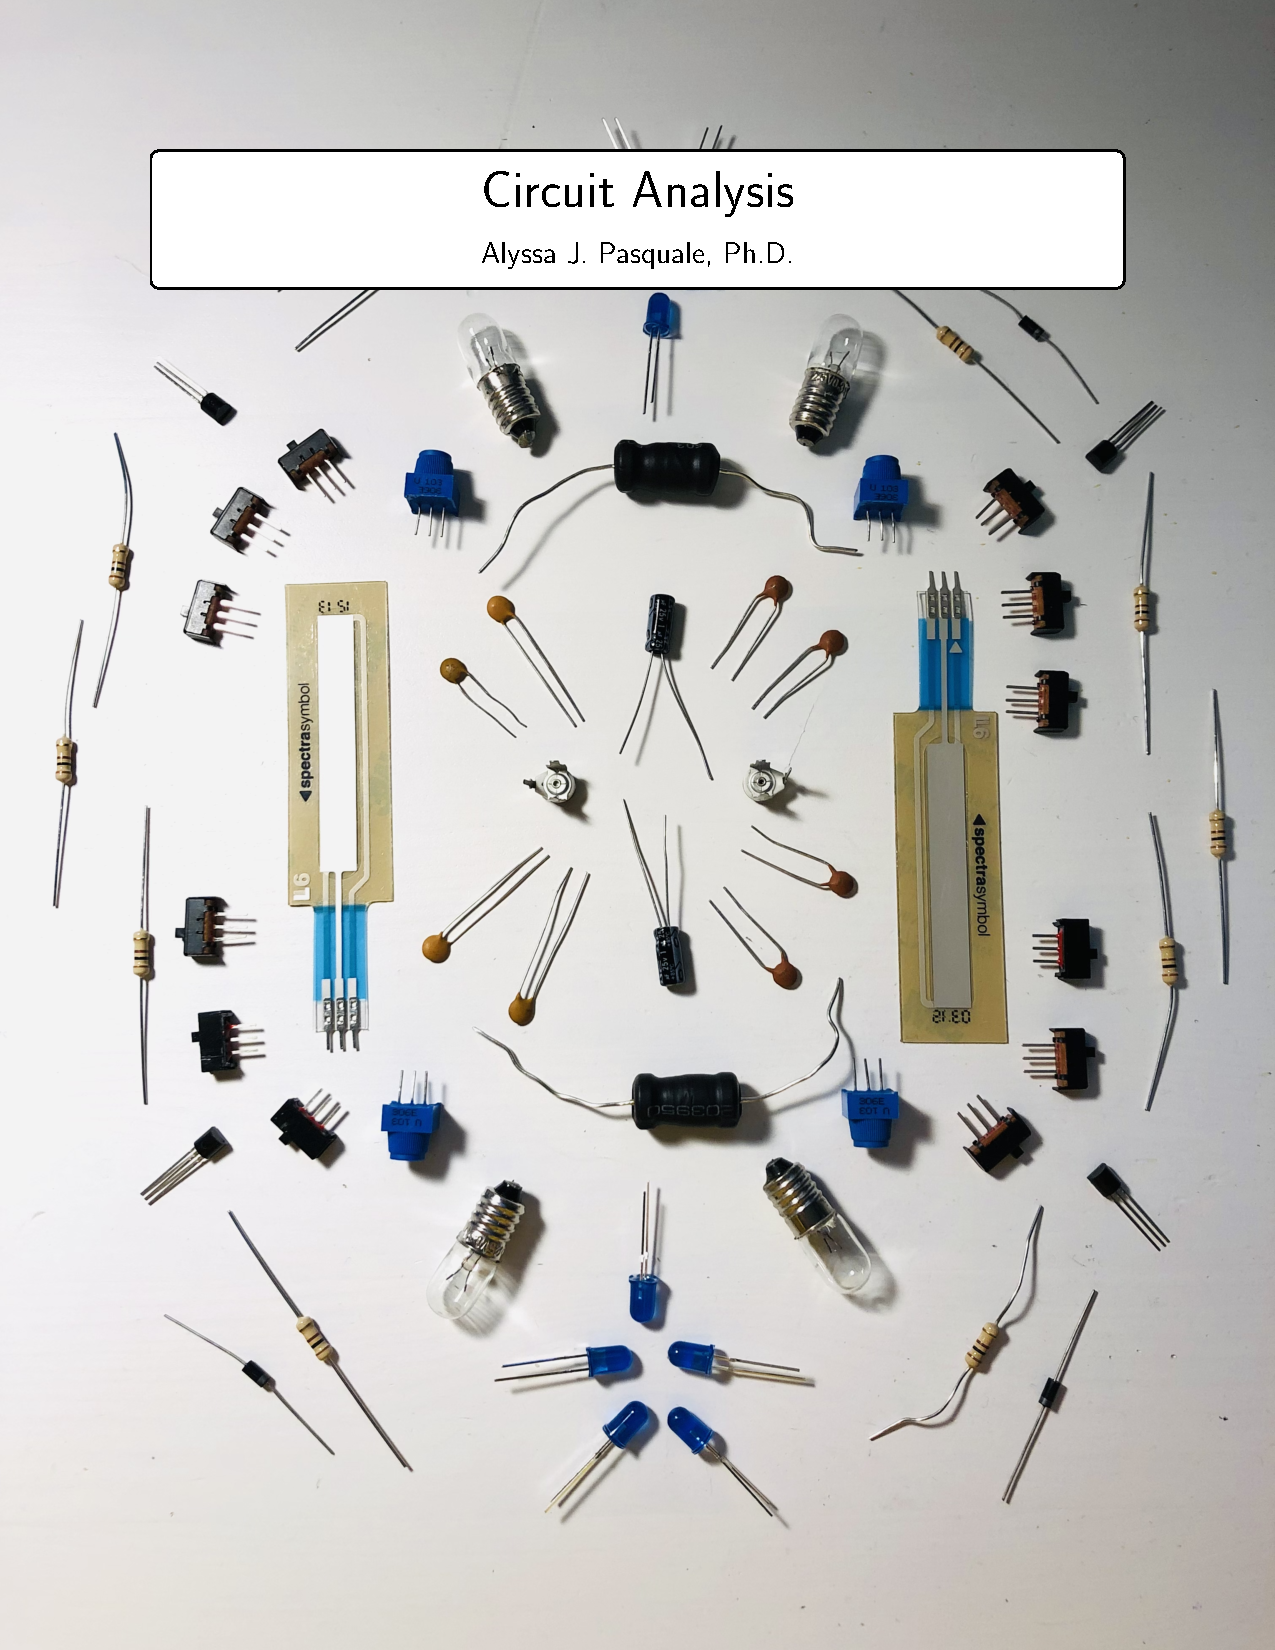
\includepdf[noautoscale=false]{external/frontcover.pdf}%
\frontmatter
%% begin: half-title
\thispagestyle{empty}
{\titlepagefont\centering
\vspace*{0.28\textheight}
{\Huge Circuit Analysis}\\}
\clearpage
%% end:   half-title
%% begin: title page
%% Inspired by Peter Wilson's "titleDB" in "titlepages" CTAN package
\thispagestyle{empty}
{\titlepagefont\centering
\vspace*{0.14\textheight}
%% Target for xref to top-level element is ToC
\addtocontents{toc}{\protect\hypertarget{my-great-book}{}}
{\Huge Circuit Analysis}\\[3\baselineskip]
{\Large Alyssa J. Pasquale, Ph.D.}\\[0.5\baselineskip]
{\Large College of DuPage}\\[3\baselineskip]
{\Large September 16, 2026}\\}
\clearpage
%% end:   title page
%% begin: copyright-page
\thispagestyle{empty}
\hypertarget{front-colophon}{}\vspace*{\stretch{2}}
\noindent{\bfseries Website}: \href{https://doctor-pasquale.com}{doctor-pasquale.com}\par\medskip
\noindent\textcopyright{}2021\textendash{}2026\quad{}Alyssa J. Pasquale, Ph.D.\\[0.5\baselineskip]
This book is licensed under creative commons as CC-BY-SA-NC. This license allows reusers to distribute, remix, adapt, and build upon the material in any medium or format for noncommercial purposes only, and only so long as attribution is given to the creator. If you remix, adapt, or build upon the material, you must license the modified material under identical terms. For more information, visit \href{https://creativecommons.org}{https:\slash{}\slash{}creativecommons.org}.%
 \par
This license (CC-BY-SA-NC) includes the following elements:%
 %
\begin{itemize}[label=\ptxlistdisc]
\item{}BY - Credit must be given to the creator%
\item{}NC - Only noncommercial uses of the work are permitted%
\item{}SA - Adaptations must be shared under the same terms%
\end{itemize}
 The suggested attribution for this book is Circuit Analysis by Alyssa J. Pasquale, Ph.D., College of DuPage, is licensed under CC BY-NC-SA 4.0.%
 \par
The entirety of this work was created by Alyssa J. Pasquale, Ph.D. The cover photograph is by the author and is a collection of circuit components (capacitors, trimmer pots, trimmer capacitors, soft potentiometers, inductors, toggle switches, transistors, resistors, diodes, light-emitting diodes, and incandescent lamps). All circuit diagrams, equations, and figures in this text were created by the author using LaTeX libraries.%
\par\medskip
\vspace*{\stretch{1}}
\null\clearpage
%% end:   copyright-page
%
%
\typeout{************************************************}
\typeout{Preface  Preface}
\typeout{************************************************}
%
\begin{preface}{Preface}{Preface}{}{Preface}{}{}{preface}
\begin{paragraphs}{Purpose.}{preface-1}%
This book was written for students taking Circuit Analysis (ENGIN-2210) at the College of DuPage. The book was originally written using my lecture notes as my template. Eventually it was adapted into a book using PreTeXt. I want students to have a free resource that they can use instead of paying hundreds of dollars for a book that they may not read and does not align exactly with my course content.%
\par
You do not have to be a COD student to use this textbook. All uses that abide by the license (refer to this book's colophon for license information) are allowed and encouraged.%
\end{paragraphs}%
\begin{paragraphs}{Note to readers.}{preface-2}%
This book will always be a work in progress. I make frequent revisions based on student feedback and issues I see students struggle with in class.%
\par
I cannot guarantee that this book is free from typos. I will, however, do my best to implement your feedback if you find any issues with the text. Feel free to e-mail me at pasqualea185@cod.edu with your notes.%
\end{paragraphs}%
\begin{paragraphs}{Note to faculty.}{preface-3}%
You are free to adapt or use this book for your class, provided you follow the Creative Commons guidelines expressed in this book's colophon. Additional information, including ancillary materials, are available \href{https://doctor-pasquale.com/books/}{\nolinkurl{on the books page of my website}}.%
\end{paragraphs}%
\begin{paragraphs}{Note on generative AI.}{preface-4}%
Generative AI was \ptxalert{not used} in any part of the process of writing or editing this book.%
\end{paragraphs}%
\begin{paragraphs}{Symbols.}{preface-5}%
DC quantities will be represented by capital letters such as \(V\) for voltage, \(I\) for current, and \(P\) for power. Time-varying quantities will be represented by lowercase letters such as \(v(t)\) for voltage, \(i(t)\) for current, and \(p(t)\) for power.%
\end{paragraphs}%
\begin{paragraphs}{Precision.}{preface-6}%
Examples in this textbook have been worked out with a TI-83+ graphing calculator, as well as with calculating software such as Matlab and Microsoft Excel. Final answers are rounded to three significant digits. It's possible that your answers may be slightly different due to rounding errors. This does not mean that you are solving a problem incorrectly.%
\end{paragraphs}%
\end{preface}
%% begin: table of contents
%% Adjust Table of Contents
\setcounter{tocdepth}{1}
\renewcommand*\contentsname{Contents}
\tableofcontents
%% end:   table of contents
\mainmatter
%
%
\typeout{************************************************}
\typeout{Chapter 1 Properties of Electric Circuits}
\typeout{************************************************}
%
\begin{chapterptx}{Chapter}{Properties of Electric Circuits}{}{Properties of Electric Circuits}{}{}{ch1-properties}
\renewcommand*{\chaptername}{Chapter}
\begin{introduction}{}%
Electric circuits have many different properties. Some of these properties describe quantities that we are interested in measuring in a circuit. Properties such as voltage and current are things that engineers are interested in designing circuits around; we want circuits to have particular values of voltage or current at specific points in a design. It's important for engineers to have a solid understanding of these properties. They will form the basis for the remainder of the content of this textbook.%
\end{introduction}%
%
%
\typeout{************************************************}
\typeout{Section 1.1 Charge}
\typeout{************************************************}
%
\begin{sectionptx}{Section}{Charge}{}{Charge}{}{}{ch1-charge}
\ptxterminology{Charge} is a fundamental property of matter just as mass is a fundamental property of matter. Charge is important because it interacts through electromagnetic forces. By physically separating two or more charges, an electric field is generated that creates either attractive or repulsive forces. These forces can direct the movement of charges throughout a circuit.%
\par
Charge comes from protons and electrons. Protons each contain one unit of positive charge (usually denoted as \(+e\)), which is equal to \(1.6\times 10^{-19}~\textrm{C}\). C stands for coulomb, which is the SI unit used for charge. Electrons each contain one unit of negative charge, which is equal to \(-1.6\times 10^{-19}~\textrm{C}\). The symbol used for charge is \(Q\).%
\begin{remark}{Remark}{Summary of charge.}{ch1-charge-4}%
%
\begin{itemize}[label=\ptxlistdisc]
\item{}Symbol: \(Q\)%
\item{}Unit: C (coulomb)%
\end{itemize}
%
\end{remark}
\end{sectionptx}
%
%
\typeout{************************************************}
\typeout{Section 1.2 Voltage}
\typeout{************************************************}
%
\begin{sectionptx}{Section}{Voltage}{}{Voltage}{}{}{ch1-voltage}
\begin{introduction}{}%
\ptxterminology{Voltage}, also referred to as electric potential, potential difference, or electromotive force, is another important property of circuits. Voltage defines how much work is done per unit of charge to move a test charge between two points. While voltage can be an abstract property to understand, it is one of the three most important properties of electric circuits (they are: voltage, current, and resistance). The symbol used for voltage is \(V\) and the unit is V (volt).%
\begin{remark}{Remark}{Summary of voltage.}{ch1-voltage-2-2}%
%
\begin{itemize}[label=\ptxlistdisc]
\item{}Symbol: \(V\)%
\item{}Unit: V (volt)%
\end{itemize}
%
\end{remark}
A useful way to understand voltage can be to compare it with its gravitational equivalent. While gravitational forces and electromagnetic forces have many differences, they also have many similarities. Gravitational potential energy describes the amount of energy that an object has by virtue of its mass and its distance away from a reference mass. However, if that object were to disappear, the reference mass would still exist, and that reference mass has the \emph{potential} to generate energy if an object of mass were to find itself some distance (\(r\)) away from the reference mass. This is depicted schematically in \hyperref[gravitationalpotential]{Figure~{\xreffont\ref{gravitationalpotential}}}. This \emph{potential} to have energy is known as gravitational potential.%
\begin{figureptx}{Figure}{Schematic depiction of gravitational potential energy and gravitational potential.}{gravitationalpotential}{}%
\begin{image}{0}{1}{0}{}%
\resizebox{\linewidth}{!}{%
\begin{tikzpicture}[font=\sffamily]
	\node[align=left, anchor=south west] at (-2,3) {$GPE = Gmm_1/r$};
	\draw[] (-2,0) -- (2,0);
	\fill[pattern = north east lines] (-2,-1) rectangle (2,0);
	\node[fill=white, align=center] at (0,-0.5) {reference object of mass $m$};
	\draw[thick] (-1.5,0) rectangle (0.5,2);
	\draw[thick] (-0.25,2) rectangle (0.5,2.75);
	\node at (0.175,2.375) {$m_1$};
	\draw[thick,Stealth-Stealth] (1,0) -- (1,2);
	\fill[white] (0.75,0.75) rectangle (1.25,1.25);
	\node at (1,1) {$r$};
	\node[align=left, anchor=south west] at (5,3) {$GP = Gm/r$};
	\draw[] (5,0) -- (9,0);
	\fill[pattern = north east lines] (5,-1) rectangle (9,0);
	\node[fill=white, align=center] at (7,-0.5) {reference object of mass $m$};
	\draw[thick] (5.5,0) rectangle (7.5,2);
	\draw[thick,Stealth-Stealth] (8,0) -- (8,2);
	\fill[white] (7.75,0.75) rectangle (8.25,1.25);
	\node at (8,1) {$r$};
\end{tikzpicture}%
}%
\end{image}%
\tcblower
\end{figureptx}%
As humans living on the planet Earth, gravitational potential depends on the mass of the Earth, the radius of the Earth, and the universal gravitational constant (\(G = 6.7 \times 10^{-11}~\textrm{Nm}^2/\textrm{kg}^2\)). While gravitational potential energy is a concept that you have probably studied extensively in your physics classes, you have probably not spent as much time on gravitational potential.%
\par
\ptxterminology{Electric potential energy} describes the energy that an object has by virtue of its charge and its distance away from a reference charge. However, if that object were to disappear, the reference charge would still exist, and that reference charge has the \emph{potential} to generate energy if an object of charge were to find itself some distance (\(r\)) away from the reference charge. This is depicted schematically in \hyperref[electricpotential]{Figure~{\xreffont\ref{electricpotential}}}. This potential to have energy is known as electric potential, or voltage.%
\begin{figureptx}{Figure}{Schematic depiction of electric potential energy and electric potential (voltage).}{electricpotential}{}%
\begin{image}{0}{1}{0}{}%
\resizebox{\linewidth}{!}{%
\begin{tikzpicture}[font=\sffamily]
	\node[align=left, anchor=south west] at (-2.5,1) {$EPE = kqq_1/r$};
	\draw[thick] (-2,0) circle (0.25);
	\node at (-2,0) {$q$};
	\draw[thick] (2,0) circle (0.25);
	\node at (2,0) {$q_1$};
	\draw[thick,Stealth-Stealth] (-2,0.5) -- (2,0.5);
	\fill[white] (-0.25,0.25) rectangle (0.25,0.75);
	\node at (0,0.5) {$r$};
	\node[align=left, anchor=south west] at (4.5,1) {$EP = kq/r$};
	\draw[thick] (5,0) circle (0.25);
	\node at (5,0) {$q$};
	\draw[thick,Stealth-Stealth] (5,0.5) -- (9,0.5);
	\fill[white] (6.75,0.25) rectangle (7.25,0.75);
	\node at (7,0.5) {$r$};
\end{tikzpicture}%
}%
\end{image}%
\tcblower
\end{figureptx}%
Voltage therefore depends on the charge of the reference object, the distance between the two objects, as well as Coulomb's constant (\(k = 8.99 \times 10^9~\textrm{Nm}^2/\textrm{C}^2\)).%
\par
What is important in the context of circuit analysis is where voltage comes from and how it will be treated as a quantity. Voltage can be generated in several different ways. Static electric fields are generated by physically separating charges and keeping them apart from each other, which is what a battery accomplishes using chemical means. Voltage can also be created by a time-varying magnetic field or charges moving through a static magnetic field. These methods are how generators and power plants work.%
\par
In an electromagnetic physics class, the emphasis is generally on using Maxwell's equations to solve for voltage as a quantity. In electrical engineering, we will treat voltage as either a source that is applied to a circuit (by means of a power supply, batteries, or function generator) or as a quantity to be measured over various circuit elements.%
\end{introduction}%
%
%
\typeout{************************************************}
\typeout{Subsection 1.2.1 Voltage as a Difference}
\typeout{************************************************}
%
\begin{subsectionptx}{Subsection}{Voltage as a Difference}{}{Voltage as a Difference}{}{}{ch1-voltagedifference}
It is important to note that voltage is a potential \emph{difference.} This implies that voltage must be measured with respect to two points in a circuit. The terminology used in this book is to mention the \textquotedblleft{}voltage dropped over an element.\textquotedblright{} Voltage is also \emph{relative,} which means that care needs to be taken in the measurement or calculation of voltage drops. In other words, measuring the voltage drop with voltmeter leads in one orientation will lead to the negative value of the measurement with the leads in the other orientation. (In mathematical terms, \(V_{ab} = - V_{ba}\).) Because voltage is relative, it is important to keep in mind what the reference is when understanding what is meant by a positive or a negative voltage drop.%
\par
It is also important to discuss the concept of a reference potential. Generally, we use \ptxterminology{ground} as a reference potential of zero volts. The symbol for ground that is used on a circuit diagram resembles an upside-down tree and is depicted in \hyperref[groundsymbol]{Figure~{\xreffont\ref{groundsymbol}}}.%
\begin{figureptx}{Figure}{Circuit symbol used for ground.}{groundsymbol}{}%
\begin{image}{0.475}{0.05}{0.475}{}%
\resizebox{\linewidth}{!}{%
\begin{tikzpicture}[font=\sffamily]
	\draw (0,0) to [short] (0,-0.1) node[ground] {};
\end{tikzpicture}%
}%
\end{image}%
\tcblower
\end{figureptx}%
The Earth serves as a good choice of zero potential (ground) in circuits. The Earth can absorb very large amounts of charge without experiencing a change in this potential. Equipment with Earth ground connections will typically have a copper wire that is buried into the Earth in order to facilitate this ability to transfer charge.%
\par
Some objects (such as cars, airplanes, and some consumer electronic devices with portable power sources) do not have a physical connection to Earth ground, but still make use of a reference voltage of zero potential. For example, an airplane will typically use the metal chassis as a ground. However, this can lead to static buildup as charge cannot always dissipate from the metal chassis. When an airplane is refueled, this can be a particular hazard. For this reason, a fuel truck will ground itself to the airplane chassis to reduce any possibility of static buildup and discharge. Electrostatic discharge can also be a hazard when using integrated circuits, particularly those used for assembling computers. Care and consideration must be taken to ensure that people are properly grounded before and during working with these objects.%
\end{subsectionptx}
%
%
\typeout{************************************************}
\typeout{Subsection 1.2.2 Measuring Voltage}
\typeout{************************************************}
%
\begin{subsectionptx}{Subsection}{Measuring Voltage}{}{Measuring Voltage}{}{}{ch1-measuringvoltage}
Voltage can be measured in a circuit using a device called a \ptxterminology{voltmeter}. (A device that can measure multiple properties \textemdash{} such as voltage, current, and resistance \textemdash{} is called a multimeter.) The circuit symbol for a voltmeter is shown in \hyperref[voltmeter]{Figure~{\xreffont\ref{voltmeter}}}. A voltmeter contains two leads: a positive and a reference (or common) lead. When placed across the elements of a circuit, the potential difference between the two points (potential at positive lead minus the potential at common lead) is measured. Modern digital voltmeters typically use analog to digital converters and microcontrollers to turn a voltage measurement into a digital readout. Note that it is important to establish the reference potential and ensure that the leads are placed with the correct orientation. Otherwise, the voltmeter will display the negative of the desired value. (\(V_{ab} = - V_{ba}\).)%
\begin{figureptx}{Figure}{Circuit symbol used for a voltmeter.}{voltmeter}{}%
\begin{image}{0.425}{0.15}{0.425}{}%
\resizebox{\linewidth}{!}{%
\begin{tikzpicture}[font=\sffamily]
	\draw (0,0) to [rmeter, t=V] (2,0);
\end{tikzpicture}%
}%
\end{image}%
\tcblower
\end{figureptx}%
Due to Kirchhoff's voltage law (introduced in \hyperref[ch2-kvl]{Subsection~{\xreffont\ref{ch2-kvl}}}), voltages must be measured in parallel. In other words, if the voltage drop over a particular circuit element is to be measured, then one lead of the voltmeter should be on one end of the element with the other lead of the voltmeter on the other end of the element. This is shown graphically in \hyperref[measuringvoltage]{Figure~{\xreffont\ref{measuringvoltage}}}.%
\begin{figureptx}{Figure}{A diagram of how voltage is measured in parallel (across a component).}{measuringvoltage}{}%
\begin{image}{0.35}{0.3}{0.35}{}%
\resizebox{\linewidth}{!}{%
\begin{tikzpicture}[font=\sffamily]
	\draw (0.5,1.5) to [qvprobe] (3.5,1.5);
	\draw[-Stealth] (0.5,1.5) -- (0.5,0);
	\draw[-Stealth] (3.5,1.5) -- (3.5,0);
	\draw (0,0) to [generic] (4,0);
\end{tikzpicture}%
}%
\end{image}%
\tcblower
\end{figureptx}%
It is important for a measuring tool to provide minimal impact on the functionality of a circuit. Because a voltmeter is placed in parallel with a circuit element, it is important for current into the voltmeter to be minimal. If current were to flow into the voltmeter, then it would change the current through the circuit and would impact the measurement of the voltage. For this reason, voltmeters are designed with a very high internal resistance. (Resistance is a concept that will be introduced in \hyperref[ch2-resistor]{Section~{\xreffont\ref{ch2-resistor}}}.) This makes voltmeters rather safe to use, as placing a voltmeter incorrectly cannot lead to an accidental low-resistance short circuit.%
\end{subsectionptx}
\end{sectionptx}
%
%
\typeout{************************************************}
\typeout{Section 1.3 Current}
\typeout{************************************************}
%
\begin{sectionptx}{Section}{Current}{}{Current}{}{}{ch1-current}
\begin{introduction}{}%
\ptxterminology{Current} quantifies the amount of charge moving past a point per unit of time; if charge changes with time, then current is equal to the time derivative of charge, defined in \hyperref[ch1-currentequation]{({\xreffont\ref{ch1-currentequation}})}. The symbol for current is \(I\).%
\par
%
\begin{equation}
i(t) = \frac{dq(t)}{dt}\label{ch1-currentequation}
\end{equation}
%
\par
Because the unit of charge is C (coulomb) and the unit of time is s (second), the unit for current is C\slash{}s (coulombs per second), also known as A (ampere or amp).%
\begin{remark}{Remark}{Summary of current.}{ch1-current-2-4}%
%
\begin{itemize}[label=\ptxlistdisc]
\item{}Symbol: \(I\)%
\item{}Unit: A (amp)%
\end{itemize}
%
\end{remark}
Negatively charged particles will move through a conductor in the presence of an electric field to an area of high potential (positive charge). Current is defined opposite to the motion of negative charges. In other words: \ptxalert{current is defined opposite to the motion of electrons in a circuit}.%
\par
\ptxalert{Current will only flow through a closed circuit.} That is, there must be a complete path for electrons to move. Current will be zero through any circuit (or circuit branch) that is not closed. \hyperref[open-and-closed-circuit]{Figure~{\xreffont\ref{open-and-closed-circuit}}} depicts an open circuit (left) and a closed circuit (right).%
\begin{figureptx}{Figure}{An open circuit (left) and a closed circuit (right).}{open-and-closed-circuit}{}%
\begin{image}{0.1}{0.8}{0.1}{}%
\resizebox{\linewidth}{!}{%
\begin{tikzpicture}[font=\sffamily]
	\draw[]	(0,2.5) to [V, l_=$V_S$]	(0,0);
	\draw[]	(0,2.5) to [generic]		(2.5,2.5);
	\draw[]	(0,0) to [short]			(2.5,0);
	\draw[]	(5,2.5) to [V, l_=$V_S$]	(5,0);
	\draw[]	(5,2.5) to [generic]		(7.5,2.5);
	\draw[]	(7.5,2.5) to [short] 		(7.5,0) --++ (left:2.5);
\end{tikzpicture}%
}%
\end{image}%
\tcblower
\end{figureptx}%
\end{introduction}%
%
%
\typeout{************************************************}
\typeout{Subsection 1.3.1 Current as a Flow}
\typeout{************************************************}
%
\begin{subsectionptx}{Subsection}{Current as a Flow}{}{Current as a Flow}{}{}{ch1-currentflow}
Current relates to the flow of charge through an object. Because the charge is moving in a particular direction, the sign of current correlates to the direction of the current. It is possible to calculate or measure current in any arbitrary direction. If the calculation or measurement yields a positive result, it means that the direction that was chosen is indeed the direction in which current is flowing. If the calculation or measurement yields a negative result, it means that current is flowing in the opposite direction.%
\par
As an example, let's assume that we have a circuit element and we believe that current is traveling from left to right, as shown in \hyperref[currentdirectionexample]{Figure~{\xreffont\ref{currentdirectionexample}}}. If we measure or calculate the current and obtain a positive result, it means that the current is indeed flowing from left to right. However, if our measurement or calculation leads to a negative result, it means that the current is flowing from right to left.%
\begin{figureptx}{Figure}{A circuit element; we are assuming that current flows from left to right.}{currentdirectionexample}{}%
\begin{image}{0.35}{0.3}{0.35}{}%
\resizebox{\linewidth}{!}{%
\begin{tikzpicture}[font=\sffamily]
	\draw (0,0) to [generic, f_=$I$] (4,0);
\end{tikzpicture}%
}%
\end{image}%
\tcblower
\end{figureptx}%
\end{subsectionptx}
%
%
\typeout{************************************************}
\typeout{Subsection 1.3.2 Measuring Current}
\typeout{************************************************}
%
\begin{subsectionptx}{Subsection}{Measuring Current}{}{Measuring Current}{}{}{ch1-measuringcurrent}
Current can be measured in a circuit using a device called an \ptxterminology{ammeter}. The circuit schematic for an ammeter is shown in \hyperref[ammeter]{Figure~{\xreffont\ref{ammeter}}}. An ammeter contains two leads. Current enters through one lead and exits through the reference (common) lead. When placed in series with a circuit element, the current through the ammeter is measured. An ammeter will measure the current flowing from one lead to the common lead; therefore it is important to verify the orientation of the leads to ensure that the readout is not going to be the negative value of what is desired.%
\begin{figureptx}{Figure}{Circuit symbol used for an ammeter.}{ammeter}{}%
\begin{image}{0.425}{0.15}{0.425}{}%
\resizebox{\linewidth}{!}{%
\begin{tikzpicture}[font=\sffamily]
	\draw (0,0) to [rmeter, t=A] (2,0);
\end{tikzpicture}%
}%
\end{image}%
\tcblower
\end{figureptx}%
Modern digital ammeters use a resistor with a very small value (called a shunt resistor) over which the voltage can be measured using an analog to digital converter. Using Ohm's law, the current can be calculated using a microcontroller and displayed on a screen.%
\par
Due to Kirchhoff's current law (explained in \hyperref[ch2-kcl]{Subsection~{\xreffont\ref{ch2-kcl}}}), currents must be measured in series. In other words, the path of the circuit must be broken open, and the ammeter must be inserted into that path in order to measure the current through that path. This is shown graphically in \hyperref[measuringcurrentseries]{Figure~{\xreffont\ref{measuringcurrentseries}}}.%
\begin{figureptx}{Figure}{A diagram of how current is measured in series (in the same path as a component).}{measuringcurrentseries}{}%
\begin{image}{0.3}{0.4}{0.3}{}%
\resizebox{\linewidth}{!}{%
\begin{tikzpicture}[font=\sffamily]
	\draw (2,0) to [qiprobe] (4,0);
	\draw (-0.5,0) to [generic] (2,0);
\end{tikzpicture}%
}%
\end{image}%
\tcblower
\end{figureptx}%
Just as with a voltmeter, it is important for an ammeter to disturb the functionality of the circuit as little as possible. An ideal ammeter would contribute no voltage drop to the circuit. However, as a shunt resistor is required to measure current, that means the shunt resistor should have as small a value as possible. (The reason behind this will hopefully become clear once we introduce Ohm's law in \hyperref[ch2-ohmslaw]{Section~{\xreffont\ref{ch2-ohmslaw}}}.) Because the internal resistance of an ammeter is so low, it is imperative to use caution when connecting an ammeter. If a lot of current is caused to flow through an ammeter (by connecting the ammeter in a path with very low resistance, for example by connecting it in parallel with an element rather than in series with an element), then the internal circuitry can be damaged or a fuse blown.%
\end{subsectionptx}
\end{sectionptx}
%
%
\typeout{************************************************}
\typeout{Section 1.4 Power}
\typeout{************************************************}
%
\begin{sectionptx}{Section}{Power}{}{Power}{}{}{ch1-power}
\begin{introduction}{}%
Energy is lost or gained at particular rates in each element in a circuit. This rate of energy loss (or gain) is known as \ptxterminology{power}. The symbol for power is \(P\), and the unit is W (watt). In general, power is defined as the time derivative of energy or work in a circuit element (\(\frac{dw(t)}{dt}\)). The instantaneous power consumed by a circuit element is defined in \hyperref[ch1-instantaneouspower]{({\xreffont\ref{ch1-instantaneouspower}})}.%
\par
%
\begin{equation}
p(t) = i(t)v(t)\label{ch1-instantaneouspower}
\end{equation}
%
\begin{remark}{Remark}{Summary of power.}{ch1-power-2-3}%
%
\begin{itemize}[label=\ptxlistdisc]
\item{}Symbol: \(P\)%
\item{}Unit: W (watt)%
\end{itemize}
%
\end{remark}
\end{introduction}%
%
%
\typeout{************************************************}
\typeout{Subsection 1.4.1 Conservation of Power}
\typeout{************************************************}
%
\begin{subsectionptx}{Subsection}{Conservation of Power}{}{Conservation of Power}{}{}{ch1-conservationofpower}
Conservation of power, which comes from conservation of energy, is an important concept in electric circuits. This tells us that \emph{all power that is created or delivered in a circuit is equal to all of the power that is absorbed or consumed in that circuit.} Some circuit elements create or deliver power. Other circuit elements absorb power. To determine which thing (delivering or absorbing) a circuit element is doing, there are two methods to use. The first by being told what the circuit element is. Batteries, power supplies, and function generators deliver power. Resistors absorb power. (Some circuit elements neither create nor consume power. This concept will be introduced in \hyperref[ch10-acpower]{Chapter~{\xreffont\ref{ch10-acpower}}}.)%
\par
The second method is by analyzing the voltage drop over and current through a circuit element. If current flows from high potential to low potential in a circuit element, the element absorbs power. If current flows from low potential to high potential in a circuit element, the circuit delivers power.%
\begin{example}{Example}{Determining if circuit elements deliver or absorb power.}{ch1-conservationofpower-4}%
For each circuit element in \hyperref[powerdeliverorabsorb]{Figure~{\xreffont\ref{powerdeliverorabsorb}}}, determine if it delivers or absorbs power.%
\begin{figureptx}{Figure}{A circuit composed of four unknown circuit elements all connected in series.}{powerdeliverorabsorb}{}%
\begin{image}{0.25}{0.5}{0.25}{}%
\resizebox{\linewidth}{!}{%
\begin{tikzpicture}[font=\sffamily]
	\draw (0,3) to [generic, l_=A, v^=$V_A$] (0,0);
	\draw (0,3) to [generic, l^=B, v_=$V_B$, i^=$I$] (3,3);
	\draw (3,0) to [generic, l_=C, v^=$V_C$] (3,3);
	\draw (3,0) to [generic, l^=D, v_=$V_D$] (0,0);
\end{tikzpicture}%
}%
\end{image}%
\tcblower
\end{figureptx}%
Current flows from high to low potential in elements B and D: therefore B and D are absorbing power. Current flows from low to high potential in elements A and C: therefore A and C are delivering power.%
\end{example}
\end{subsectionptx}
\end{sectionptx}
%
%
\typeout{************************************************}
\typeout{Section 1.5 Power Sources}
\typeout{************************************************}
%
\begin{sectionptx}{Section}{Power Sources}{}{Power Sources}{}{}{ch1-powersources}
\begin{introduction}{}%
Power sources are used in a circuit to generate energy and distribute it to other circuit elements. The types of power supplies that are typically used in circuits include batteries, constant voltage sources, constant current sources, and function generators.%
\end{introduction}%
%
%
\typeout{************************************************}
\typeout{Subsection 1.5.1 Direct Current (DC) Sources}
\typeout{************************************************}
%
\begin{subsectionptx}{Subsection}{Direct Current (DC) Sources}{}{Direct Current (DC) Sources}{}{}{ch1-dcsources}
Some sources are \ptxterminology{direct current (DC)}, which means that the value of the current or voltage supplied by the source does not change with time. Three circuit symbols for DC power sources are shown in \hyperref[dcpowersources]{Figure~{\xreffont\ref{dcpowersources}}}.%
\begin{figureptx}{Figure}{Three types of DC power sources: a voltage source, battery, and current source.}{dcpowersources}{}%
\begin{image}{0.2}{0.6}{0.2}{}%
\resizebox{\linewidth}{!}{%
\begin{tikzpicture}[font=\sffamily]
	\foreach \x/\item/\label in {0/V/DC Voltage, 3/battery1/Battery, 6/I/DC Current} {
		\draw (\x,2) to [\item] (\x,0) node[below, align=center] {\label};
	}
\end{tikzpicture}%
}%
\end{image}%
\tcblower
\end{figureptx}%
The DC voltage symbol contains plus and minus signs. The plus sign represents the side of the supply that corresponds to high potential. The minus sign represents the side of the supply that corresponds to low potential. The battery does not contain plus or minus signs but instead has two lines: one long and one short. The long end (which is the upper line in \hyperref[dcpowersources]{Figure~{\xreffont\ref{dcpowersources}}}) corresponds to high potential, and the short end corresponds to low potential. In the symbol for a current source, the arrow depicts the direction of current (assuming that the source is properly connected in a complete circuit).%
\end{subsectionptx}
%
%
\typeout{************************************************}
\typeout{Subsection 1.5.2 Alternating Current (AC) Sources}
\typeout{************************************************}
%
\begin{subsectionptx}{Subsection}{Alternating Current (AC) Sources}{}{Alternating Current (AC) Sources}{}{}{ch1-acsources}
In \ptxterminology{alternating current (AC)} sources, the voltage or current supplied by the source varies with time. Four circuit symbols for AC power supplies are shown in \hyperref[acpowersources]{Figure~{\xreffont\ref{acpowersources}}}.%
\begin{figureptx}{Figure}{Four types of AC power sources: sinusoidal voltage, sinusoidal current, square wave, and triangular wave.}{acpowersources}{}%
\begin{image}{0.1}{0.8}{0.1}{}%
\resizebox{\linewidth}{!}{%
\begin{tikzpicture}[font=\sffamily]
	\foreach \x/\item/\label/\text in {0/sV/Sinusoidal Voltage/Vs, 3/sI/Sinusoidal Current/Is, 6/sqV/Square Wave/~, 9/tV/Triangular Wave/~} {
		\draw (\x,2) to [\item, l^=\text] (\x,0) node[below, align=center] {\label};
	}
\end{tikzpicture}%
}%
\end{image}%
\tcblower
\end{figureptx}%
The key to analyzing AC power supply circuit symbols is to look at the labels on the sources. The symbol within the circle depicts the nature of the time-varying source: sinusoidal, square wave, or triangular wave. The text or unit on the label (given in V, A, or mA) depicts if the source is a voltage source or current source. A plus sign on a circuit diagram using an AC power supply will be used to depict the high-potential end of the source. For a voltage source, the + sign depicts the high-potential end of the source. For a current source, the + sign depicts the direction of current flow. This is shown for both a voltage and current source in \hyperref[voltage-current-plus-signs]{Figure~{\xreffont\ref{voltage-current-plus-signs}}}.%
\begin{figureptx}{Figure}{The + sign on a sinusoidal voltage or current source depicts the point of high-potential of the source.}{voltage-current-plus-signs}{}%
\begin{image}{0.1}{0.8}{0.1}{}%
\resizebox{\linewidth}{!}{%
\begin{tikzpicture}[font=\sffamily]
	\draw[]	(0,2.5) node[below left] {+} to [sV, l_=$V_{AC}$]		(0,0);
	\draw[]	(0,2.5) to [generic]					(2.5,2.5);
	\draw[]	(2.5,2.5) to [generic]					(2.5,0) --++ (left:2.5);
	\draw[]	(5,2.5) node[below left] {+} to [sV, l_=$I_{AC}$]		(5,0);
	\draw[]	(5,2.5) to [generic]					(7.5,2.5);
	\draw[]	(7.5,2.5) to [generic] 					(7.5,0) --++ (left:2.5);
\end{tikzpicture}%
}%
\end{image}%
\tcblower
\end{figureptx}%
While square waves and triangular waves will be explored in this textbook, the major type of time-varying source that will be used is a sinusoidal wave. It is important to recall the anatomy of a sine wave, shown below in \hyperref[sinewave]{Figure~{\xreffont\ref{sinewave}}}.%
\begin{figureptx}{Figure}{A graph of the voltage of a sinusoidal voltage source plotted with respect to time.}{sinewave}{}%
\begin{image}{0}{1}{0}{}%
\resizebox{\linewidth}{!}{%
\begin{tikzpicture}[font=\sffamily]
	\begin{axis}[ylabel={$v(t)$~(V)}, xlabel={$t$~(ms)}, width=\linewidth, height=5cm, xmin=-0.1, xmax=20.1, xtick={0,2,...,20}, ytick={-2,0,...,2}]
	\addplot[ultra thick, samples=60, domain=0:20] {2*sin(deg(x*pi/5))};
	\draw[Stealth-Stealth] (axis cs:2.5,0) -- (axis cs:2.5,2) node[midway, anchor=west] {$V_m$};
	\draw[Stealth-Stealth] (axis cs:2.5,2.1) -- (axis cs:12.5,2.1) node[midway, anchor=north] {$T$};
	\draw[Stealth-Stealth] (axis cs:12.5,-2) -- (axis cs:12.5,2) node[midway, anchor=west] {$V_{PP}$};
				\end{axis}
\end{tikzpicture}%
}%
\end{image}%
\tcblower
\end{figureptx}%
A cosine wave is expressed mathematically as defined in \hyperref[ch1-eqcosinewaveperiod]{({\xreffont\ref{ch1-eqcosinewaveperiod}})}, \hyperref[ch1-eqcosinewavefrequency]{({\xreffont\ref{ch1-eqcosinewavefrequency}})}, and \hyperref[ch1-eqcosinewaveangularfrequency]{({\xreffont\ref{ch1-eqcosinewaveangularfrequency}})}.%
\par
%
\begin{align}
v(t) \amp = V_m \cos \left(\frac{2\pi t}{T} + \phi\right) + V_{DC}\label{ch1-eqcosinewaveperiod}\\
\amp = V_m \cos (2\pi ft + \phi) + V_{DC}\label{ch1-eqcosinewavefrequency}\\
\amp= V_m \cos (\omega t + \phi) + V_{DC}\label{ch1-eqcosinewaveangularfrequency}
\end{align}
%
\par
While the equations above are expressed in terms of voltage, they depict the same format that is used to describe current, power, or any other quantity that oscillates with respect to time. Each of the terms in the equation gives important information about the source.%
\par
%
\begin{itemize}[label=\ptxlistdisc]
\item{}\(V_m\) is the \ptxterminology{amplitude} of the source, which is defined as the maximum displacement from the equilibrium position. The unit of this quantity will be equal to the unit of the parameter being measured (V, A, W, etc.).%
\item{}\(V_{PP}\), while not part of the equation, describes the \ptxterminology{peak-to-peak} value of the source. This is equal to twice the amplitude, or the difference between the maximum and minimum values. The unit of this quantity will be equal to the unit of the parameter being measured (V, A, W, etc.).%
\item{}\(V_{DC}\) is a constant (DC) value added to a cosine wave if the equilibrium of the wave is not equal to zero. This parameter is known as the \ptxterminology{DC offset} of the wave. The unit of this quantity will be equal to the unit of the parameter being measured (V, A, W, etc.).%
\item{}\(T\) is equal to the \ptxterminology{period} of the wave, which describes how long it takes for one oscillation to occur. The unit used for period is s (second).%
\item{}\(f\) is the wave \ptxterminology{frequency}. This is the inverse of period, defined in \hyperref[ch1-periodfrequency]{({\xreffont\ref{ch1-periodfrequency}})}, and describes how many oscillations occur per unit of time. The unit used for frequency is Hz (hertz).%
\item{}\(\omega\) is equal to the \ptxterminology{angular frequency} of the wave. The relationship between frequency and angular frequency is defined in \hyperref[ch1-angularvsnormalfrequency]{({\xreffont\ref{ch1-angularvsnormalfrequency}})}. The unit used for angular frequency is rad\slash{}s (radians per second).%
\item{}\(\phi\) is the \ptxterminology{phase} of the wave. It describes the angular offset of the start of the wave. The unit used for phase is rad (radian).%
\end{itemize}
%
\par
%
\begin{equation}
f = \frac{1}{T}\label{ch1-periodfrequency}
\end{equation}
%
\par
%
\begin{equation}
\omega = 2 \pi f\label{ch1-angularvsnormalfrequency}
\end{equation}
%
\par
To convert between degrees and radians, the conversion factor in \hyperref[ch1-radian-to-degree-conversion]{({\xreffont\ref{ch1-radian-to-degree-conversion}})} can be applied.%
\par
%
\begin{equation}
180~^\circ = \pi~\textrm{rad}\label{ch1-radian-to-degree-conversion}
\end{equation}
%
\end{subsectionptx}
%
%
\typeout{************************************************}
\typeout{Subsection 1.5.3 Dependent Sources}
\typeout{************************************************}
%
\begin{subsectionptx}{Subsection}{Dependent Sources}{}{Dependent Sources}{}{}{ch1-dependentsources}
All of the sources described in the previous two subsections are independent sources. That is, the values of the sources are independent of any other property or characteristic of the circuit. This is the type of source that you would expect when using a power supply or a battery that has a given voltage rating. It doesn't matter what values exist elsewhere in the circuit; a AA battery will always supply a voltage of 1.5~V.%
\par
This subsection describes \ptxterminology{dependent sources}. These sources deliver voltage and current proportionally to other circuit characteristics. It is important to note that dependent sources aren't generally describing something that you can buy and put into a circuit (such as a battery) but are used to model otherwise complicated circuit elements (such as operational amplifiers and transistors).%
\par
There are four types of dependent sources. The circuit symbols are shown in \hyperref[dependentsourcesfigure]{Figure~{\xreffont\ref{dependentsourcesfigure}}}. Note that whereas independent sources are circular, dependent sources are diamond shaped.%
\begin{figureptx}{Figure}{The four types of dependent sources: voltage-controlled voltage source (VCVS), voltage-controlled current source (VCCS), current-controlled voltage source (CCVS), and current-controlled current source (CCCS).}{dependentsourcesfigure}{}%
\begin{image}{0.1}{0.8}{0.1}{}%
\resizebox{\linewidth}{!}{%
\begin{tikzpicture}[font=\sffamily]
	\foreach \x/\item/\label/\text in {0/cV/VCVS/{$k\cdot V_c$}, 3/cI/VCCS/{$g_m \cdot V_c$}, 6/cV/CCVS/{$r_m\cdot I_c$}, 9/cI/CCCS/{$k_i \cdot I_c$}} {
		\draw (\x,2) to [\item, l_=\text] (\x,0) node[below, align=center] {\label};
	}
\end{tikzpicture}%
}%
\end{image}%
\tcblower
\end{figureptx}%
Each dependent source has a magnitude that's equal to a proportionality constant multiplied by a controlling value. Each of these values is described in \hyperref[ch1-tableofdependentsources]{Table~{\xreffont\ref{ch1-tableofdependentsources}}}.%
\begin{tableptx}{Table}{\textbf{Descriptions of the magnitude, proportionality constant, and controlling value for each type of dependent source}}{ch1-tableofdependentsources}{}%
\begin{tabularbox}{0}{1}{0}%
\resizebox{\ifdim\width > \linewidth\linewidth\else\width\fi}{!}{%
{\tabularfont%
\begin{tabular}{llll}
\multicolumn{1}{m{0.35\linewidth}}{\raggedright%
Source Type%
}&\multicolumn{1}{m{0.2\linewidth}}{\raggedright%
Magnitude%
}&\multicolumn{1}{m{0.25\linewidth}}{\raggedright%
Proportionality Constant%
}&\multicolumn{1}{m{0.2\linewidth}}{\raggedright%
Controlling Value%
}\tabularnewline\ptxhrulemedium
\multicolumn{1}{m{0.35\linewidth}}{\raggedright%
Voltage-controlled voltage source (VCVS)%
}&\(V_d\) (V)&\(k\) (unitless)&\(V_c\) (V)\tabularnewline\ptxhrulethin
\multicolumn{1}{m{0.35\linewidth}}{\raggedright%
Voltage-controlled current source (VCCS)%
}&\(I_d\) (A)&\(g_m\) (A\slash{}V)&\(V_c\) (V)\tabularnewline\ptxhrulethin
\multicolumn{1}{m{0.35\linewidth}}{\raggedright%
Current-controlled voltage source (CCVS)%
}&\(V_d\) (V)&\(r_m\) (V\slash{}A, Ω)&\(I_c\) (A)\tabularnewline\ptxhrulethin
\multicolumn{1}{m{0.35\linewidth}}{\raggedright%
Current-controlled current source (CCCS)%
}&\(I_d\) (A)&\(k_i\) (unitless)&\(I_c\) (A)\tabularnewline\ptxhrulethin
\end{tabular}
}%
}%
\end{tabularbox}%
\end{tableptx}%
\end{subsectionptx}
%
%
\typeout{************************************************}
\typeout{Subsection 1.5.4 Equivalent Sources}
\typeout{************************************************}
%
\begin{subsectionptx}{Subsection}{Equivalent Sources}{}{Equivalent Sources}{}{}{ch1-equivalentsources}
If a circuit contains multiple sources (whether they be DC or AC; dependent or independent), it may be possible to combine sources together into an equivalent source. This is the first tool that we can use to help simplify circuits.%
\par
Voltage sources can be added together if they are in series with each other. If there are any other components between the sources, then the sources can still be added together as long as every circuit component is in series. \ptxalert{If it is necessary to measure the voltage at a node in between sources, then the sources should not be combined.}%
\begin{example}{Example}{Combining voltage sources that are in series.}{ch1-equivalentsources-4}%
Reduce the circuit shown in \hyperref[exampletwoseriesvoltages]{Figure~{\xreffont\ref{exampletwoseriesvoltages}}} to a circuit with a single voltage source.%
\begin{figureptx}{Figure}{A circuit consisting of two independent DC voltage sources.}{exampletwoseriesvoltages}{}%
\begin{image}{0.35}{0.3}{0.35}{}%
\resizebox{\linewidth}{!}{%
\begin{tikzpicture}[font=\sffamily]
	\draw (0,2) to [V, l_=5~V, -o] (0,0) node[below] {b};
	\draw (0,2) to [V, l^=2~V, -o] (2,2) node[right] {a};
\end{tikzpicture}%
}%
\end{image}%
\tcblower
\end{figureptx}%
The two voltage sources can be combined because they are in series with each other. The total voltage drop between nodes a and b is \(-2~\textrm{V} + 5~\textrm{V} = 3~\textrm{V}\). The two voltage sources can therefore be combined into a single voltage source with the equivalent voltage of 3~V. This is depicted in \hyperref[exampletwoseriesvoltagesafter]{Figure~{\xreffont\ref{exampletwoseriesvoltagesafter}}}.%
\begin{figureptx}{Figure}{A circuit consisting of a single independent DC voltage source.}{exampletwoseriesvoltagesafter}{}%
\begin{image}{0.425}{0.15}{0.425}{}%
\resizebox{\linewidth}{!}{%
\begin{tikzpicture}[font=\sffamily]
	\draw (6,2) node[above] {a} to [V, l_=3~V, o-o] (6,0) node[below] {b};
\end{tikzpicture}%
}%
\end{image}%
\tcblower
\end{figureptx}%
\end{example}
\begin{example}{Example}{Combining voltage sources that are in series with other components.}{ch1-equivalentsources-5}%
Reduce the circuit shown in \hyperref[exampletwoseriesvoltagesother]{Figure~{\xreffont\ref{exampletwoseriesvoltagesother}}} to a circuit with a single voltage source.%
\begin{figureptx}{Figure}{A circuit consisting of two independent DC voltage sources in series with a resistor.}{exampletwoseriesvoltagesother}{}%
\begin{image}{0.25}{0.5}{0.25}{}%
\resizebox{\linewidth}{!}{%
\begin{tikzpicture}[font=\sffamily]
	\draw (0,2) to [V, l_=1~V, -o] (0,0) node[below] {b};
	\draw (4,2) node[right] {a} to [V, l_=5~V, o-] (2,2);
	\draw (0,2) node[above] {x} to [R, l^=$R$, *-*] (2,2) node[above] {y};
\end{tikzpicture}%
}%
\end{image}%
\tcblower
\end{figureptx}%
Even though a resistor is placed between the two voltage sources, they can still be combined because the voltage sources are in series with each other. Note that if the voltage drop between node x and ground (or between node y and ground) needs to be measured, combining the voltage sources will lead to incorrect measurements. The reduced circuit is shown in \hyperref[exampletwoseriesvoltagesotherafter]{Figure~{\xreffont\ref{exampletwoseriesvoltagesotherafter}}}.%
\begin{figureptx}{Figure}{A circuit consisting of a single independent DC voltage source in series with a resistor.}{exampletwoseriesvoltagesotherafter}{}%
\begin{image}{0.325}{0.35}{0.325}{}%
\resizebox{\linewidth}{!}{%
\begin{tikzpicture}[font=\sffamily]
	\draw (8,2)to [V, l_=6~V, -o] (8,0) node[below] {b};
	\draw (8,2) to [R, l^=$R$, -o] (10,2) node[right] {a};
\end{tikzpicture}%
}%
\end{image}%
\tcblower
\end{figureptx}%
\end{example}
\begin{example}{Example}{When voltage sources cannot be combined.}{ch1-equivalentsources-6}%
\ptxalert{Possibility 1: the voltage sources are not in series}%
\par
The circuit diagram below demonstrates two voltage sources that are not in series with each other. These two sources cannot be combined together.%
\begin{figureptx}{Figure}{Circuit diagram with voltage sources that are not in series and, therefore, cannot be combined.}{ch1-equivalentsources-6-2-3}{}%
\begin{image}{0.2}{0.6}{0.2}{}%
\resizebox{\linewidth}{!}{%
\begin{tikzpicture}[font=\sffamily]
	\draw[]	(0,2.5) to [V, l_=$V_{S1}$]			(0,0);
	\draw[]	(0,2.5) to [R, l^=$R_1$]			(2.5,2.5);
	\draw[]	(2.5,2.5) to [R, l_=$R_2$, *-*]		(2.5,0);
	\draw[]	(2.5,2.5) to [R, l^=$R_3$]			(5,2.5);
	\draw[]	(5,2.5) to [V, l_=$V_{S2}$] 		(5,0);
	\draw[]	(0,0) to [short]					(5,0);
\end{tikzpicture}%
}%
\end{image}%
\tcblower
\end{figureptx}%
\ptxalert{Possibility 2: voltage needs to be measured between sources}%
\par
The circuit diagram below demonstrates two voltage sources that are in series with each other. However, a voltage needs to be measured between the two sources. These two sources should not be combined together as they will lead to an incorrect calculation of \(V_X\).%
\begin{figureptx}{Figure}{Circuit diagram with a voltage that needs to be measured between series voltage sources.}{ch1-equivalentsources-6-2-6}{}%
\begin{image}{0.2}{0.6}{0.2}{}%
\resizebox{\linewidth}{!}{%
\begin{tikzpicture}[font=\sffamily]
	\draw[]	(0,2.5) to [V, l_=$V_{S1}$]				(0,0);
	\draw[]	(0,2.5) to [R, l^=$R_1$]				(2.5,2.5);
	\draw[]	(2.5,2.5) to [R, l^=$R_2$, v_=$V_X$]	(5,2.5);
	\draw[]	(5,2.5) to [V, l_=$V_{S2}$] 			(5,0);
	\draw[]	(0,0) to [short]						(5,0);
\end{tikzpicture}%
}%
\end{image}%
\tcblower
\end{figureptx}%
\end{example}
Current sources can be added together if they are in parallel with each other. If there are any other components between the sources, the sources can still be added together as long as every circuit component is in parallel. \ptxalert{If it is necessary to measure the current through a branch in between sources, then the sources should not be combined.}%
\begin{example}{Example}{Combining current sources that are in parallel.}{ch1-equivalentsources-8}%
Reduce the circuit shown in \hyperref[exampletwoseriescurrents]{Figure~{\xreffont\ref{exampletwoseriescurrents}}} to a circuit with a single current source.%
\begin{figureptx}{Figure}{A circuit consisting of two independent DC current sources.}{exampletwoseriescurrents}{}%
\begin{image}{0.3}{0.4}{0.3}{}%
\resizebox{\linewidth}{!}{%
\begin{tikzpicture}[font=\sffamily]
	\draw (0,0) to [I, l^=2~mA] (0,2);
	\draw (2,2) to [I, l_=1~mA] (2,0);
	\draw (0,0) to [short] (2,0);
	\draw (1,0) to [short, *-o] (1,-0.5) node[below] {b};
	\draw (0,2) to [short] (2,2);
	\draw (1,2) to [short, *-o] (1,2.5) node[above] {a};
\end{tikzpicture}%
}%
\end{image}%
\tcblower
\end{figureptx}%
The two current sources can be combined because they are in parallel with each other. The current from b to a is \(2~\textrm{mA} - 1~\textrm{mA} = 1~\textrm{mA}\). The two sources can therefore be combined into a single source with the equivalent current of 1~mA. This is depicted in \hyperref[exampletwoseriescurrentsafter]{Figure~{\xreffont\ref{exampletwoseriescurrentsafter}}}.%
\begin{figureptx}{Figure}{A circuit consisting of a single independent DC current source.}{exampletwoseriescurrentsafter}{}%
\begin{image}{0.425}{0.15}{0.425}{}%
\resizebox{\linewidth}{!}{%
\begin{tikzpicture}[font=\sffamily]
	\draw (5,0) node[below] {b} to [I, l^=1~mA, o-o] (5,2) node[above] {a};
\end{tikzpicture}%
}%
\end{image}%
\tcblower
\end{figureptx}%
\end{example}
\begin{example}{Example}{Combining current sources that are in parallel with other components.}{ch1-equivalentsources-9}%
Reduce the circuit shown in \hyperref[exampletwoparallelcurrentsother]{Figure~{\xreffont\ref{exampletwoparallelcurrentsother}}} to a circuit with a single current source.%
\begin{figureptx}{Figure}{A circuit consisting of two independent DC current sources in parallel with two resistors.}{exampletwoparallelcurrentsother}{}%
\begin{image}{0.25}{0.5}{0.25}{}%
\resizebox{\linewidth}{!}{%
\begin{tikzpicture}[font=\sffamily]
	\draw (0,0) to [I, l^=5~mA] (2,0);
	\draw (0,1.25) to [R, *-*] (2,1.25);
	\draw (0,2.5) to [I, l^=6~mA, *-*] (2,2.5);
	\draw (0,3.75) to [R] (2,3.75);
	\draw (0,0) to [short] (0,3.75);
	\draw (0,1.875) to [short, *-o] (-0.5,1.875) node[left] {a};
	\draw (2,0) to [short] (2,3.75);
	\draw (2,1.875) to [short, *-o] (2.5,1.875) node[right] {b};
\end{tikzpicture}%
}%
\end{image}%
\tcblower
\end{figureptx}%
The two current sources can be combined because they are in parallel with each other. The presence of the two resistors does not change anything about the configuration of the circuit. The total current from a to b is \(6~\textrm{mA} + 5~\textrm{mA} = 11~\textrm{mA}\). The reduced circuit is shown in \hyperref[exampletwoparallelcurrentsotherafter]{Figure~{\xreffont\ref{exampletwoparallelcurrentsotherafter}}}.%
\begin{figureptx}{Figure}{A circuit consisting of a single independent DC current source in parallel with two resistors.}{exampletwoparallelcurrentsotherafter}{}%
\begin{image}{0.25}{0.5}{0.25}{}%
\resizebox{\linewidth}{!}{%
\begin{tikzpicture}[font=\sffamily]
	\draw (4.5,3.125) to [I, l^=11~mA] (6.5,3.125);
	\draw (4.5,1.875) to [R] (6.5,1.875);
	\draw (4.5,0.625) to [R] (6.5,0.625);
	\draw (4.5,0.625) to [short] (4.5,3.125);
	\draw (4.5,1.875) to [short, *-o] (4.0,1.875) node[left] {a};
	\draw (6.5,0.625) to [short] (6.5,3.125);
	\draw (6.5,1.875) to [short, *-o] (7,1.875) node[right] {b};
\end{tikzpicture}%
}%
\end{image}%
\tcblower
\end{figureptx}%
\end{example}
\begin{example}{Example}{When current sources cannot be combined.}{ch1-equivalentsources-10}%
\ptxalert{Possibility 1: the current sources are not in parallel}%
\par
The circuit diagram below demonstrates two current sources that are not in parallel with each other. These two sources cannot be combined together.%
\begin{figureptx}{Figure}{Circuit diagram with current sources that are not in parallel and, therefore, cannot be combined.}{ch1-equivalentsources-10-2-3}{}%
\begin{image}{0.1}{0.8}{0.1}{}%
\resizebox{\linewidth}{!}{%
\begin{tikzpicture}[font=\sffamily]
	\draw[]	(-2.5,0) to [I, l^=$I_{S1}$]		(-2.5,2.5);
	\draw[]	(-2.5,2.5) to [short]				(0,2.5);
	\draw[]	(0,2.5) to [R, l_=$R_1$, *-*]		(0,0);
	\draw[]	(0,2.5) to [R, l^=$R_2$]			(2.5,2.5);
	\draw[]	(2.5,2.5) to [R, l_=$R_3$, *-*]		(2.5,0);
	\draw[]	(2.5,2.5) to [short]				(5,2.5);
	\draw[]	(5,0) to [I, l^=$I_{S2}$] 			(5,2.5);
	\draw[]	(-2.5,0) to [short]					(5,0);
\end{tikzpicture}%
}%
\end{image}%
\tcblower
\end{figureptx}%
\ptxalert{Possibility 2: current needs to be measured between sources}%
\par
The circuit diagram below demonstrates two current sources that are in parallel with each other. However, a current needs to be measured between the two sources. These two sources should not be combined together as they will lead to an incorrect calculation of \(I_X\).%
\begin{figureptx}{Figure}{Circuit diagram with a current that needs to be measured between parallel current sources.}{ch1-equivalentsources-10-2-6}{}%
\begin{image}{0.1}{0.8}{0.1}{}%
\resizebox{\linewidth}{!}{%
\begin{tikzpicture}[font=\sffamily]
	\draw[]	(-2.5,0) to [I, l^=$I_{S1}$]		(-2.5,2.5);
	\draw[]	(-2.5,2.5) to [short]				(0,2.5);
	\draw[]	(0,2.5) to [R, l_=$R_1$, *-*]		(0,0);
	\draw[]	(0,2.5) to [short, i^=$I_X$]		(2.5,2.5);
	\draw[]	(2.5,2.5) to [R, l_=$R_2$, *-*]		(2.5,0);
	\draw[]	(2.5,2.5) to [short]				(5,2.5);
	\draw[]	(5,0) to [I, l^=$I_{S2}$] 			(5,2.5);
	\draw[]	(-2.5,0) to [short]					(5,0);
\end{tikzpicture}%
}%
\end{image}%
\tcblower
\end{figureptx}%
\end{example}
\end{subsectionptx}
\end{sectionptx}
%
%
\typeout{************************************************}
\typeout{Section 1.6 Elementary Signals}
\typeout{************************************************}
%
\begin{sectionptx}{Section}{Elementary Signals}{}{Elementary Signals}{}{}{ch1-elementarysignals}
\begin{introduction}{}%
Elementary signals are used to mathematically describe the types of signals used as sources, or signals that are commonly encountered in the analog circuit world. Each of the signals can be expressed mathematically.%
\end{introduction}%
%
%
\typeout{************************************************}
\typeout{Subsection 1.6.1 Dirac Delta Function}
\typeout{************************************************}
%
\begin{subsectionptx}{Subsection}{Dirac Delta Function}{}{Dirac Delta Function}{}{}{ch1-deltafunction}
The \ptxterminology{Dirac delta function} is a useful approximation of a \textquotedblleft{}spike.\textquotedblright{} It is used to model an impulse, and is commonly used in signal processing (including Fourier analysis). It is defined as a normal (Gaussian) distribution when the variance is equal to zero. The mathematical expression used to define the Dirac delta function is defined in \hyperref[ch1-diracdelta]{({\xreffont\ref{ch1-diracdelta}})},  where \(A\) is the amplitude of the function and \(\tau\) is the time at which the function occurs.%
\par
%
\begin{equation}
f(t) = A\delta(t-\tau)\label{ch1-diracdelta}
\end{equation}
%
\par
The Dirac delta function defined in \hyperref[ch1-diracdelta]{({\xreffont\ref{ch1-diracdelta}})} is depicted graphically in \hyperref[diracdeltafigure]{Figure~{\xreffont\ref{diracdeltafigure}}}.%
\begin{figureptx}{Figure}{Graphical depiction of a Dirac delta function.}{diracdeltafigure}{}%
\begin{image}{0}{1}{0}{}%
\resizebox{\linewidth}{!}{%
\begin{tikzpicture}[font=\sffamily]
	\begin{axis}[xlabel=$t$~(s), xmin=1, xmax=3, xtick={2}, xticklabel={$\tau$}, ymin=0, ymax=3, ytick={0,3}, yticklabels={0,$A$}, width=\linewidth, height=5cm, axis x line=bottom, axis y line = left]
	\addplot+[ycomb,black,thick,samples=2,domain=2:4,mark options={black}] {x+1};
				\end{axis}
\end{tikzpicture}%
}%
\end{image}%
\tcblower
\end{figureptx}%
\begin{example}{Example}{Plotting a signal composed of Dirac delta functions.}{ch1-deltafunction-6}%
Plot \(f(t) = 4\delta(t-1) - 2\delta(t+3)\). The first term has an amplitude of \(A = 4\) and is located at \(t = 1~\textrm{s}\). The second term has an amplitude of \(A = -2\) and is located at \(t = -3~\textrm{s}\). The graph is shown in \hyperref[diracdeltafunctionexample]{Figure~{\xreffont\ref{diracdeltafunctionexample}}}.%
\begin{figureptx}{Figure}{The graph of \(f(t) = 4\delta(t-1) - 2\delta(t+3)\).}{diracdeltafunctionexample}{}%
\begin{image}{0}{1}{0}{}%
\resizebox{\linewidth}{!}{%
\begin{tikzpicture}[font=\sffamily]
	\begin{axis}[xlabel=$t$~(s), ylabel=$f(t)$, xmin=-4, xmax=4, ymin=-4, ymax=4, width=\linewidth, height=5cm, axis x line=center, axis y line = left, ytick={-4,0,4}, xtick={-4,-2,...,4}]
	\addplot+[ycomb, black, thick] plot coordinates {(-3,-2) (1,4)};
				\end{axis}
\end{tikzpicture}%
}%
\end{image}%
\tcblower
\end{figureptx}%
\end{example}
The Dirac delta function has a \ptxterminology{sifting property}. It is capable of being used to determine the value of a continuous function at a certain point. This property is defined in \hyperref[ch1-sifting]{({\xreffont\ref{ch1-sifting}})}.%
\par
%
\begin{equation}
\int_{-\infty}^\infty f(t)\delta(t-a)\, dt = f(a)\label{ch1-sifting}
\end{equation}
%
\end{subsectionptx}
%
%
\typeout{************************************************}
\typeout{Subsection 1.6.2 Step Function}
\typeout{************************************************}
%
\begin{subsectionptx}{Subsection}{Step Function}{}{Step Function}{}{}{ch1-stepfunction}
The \ptxterminology{unit step function} is a piecewise function whose value is zero when the argument is negative, and equal to one when the argument is zero or positive. This function is described in \hyperref[ch1-piecewisestepfunctiondefinition]{({\xreffont\ref{ch1-piecewisestepfunctiondefinition}})}.%
\par
%
\begin{equation}
u(\tau) =
\begin{cases}
0 \amp \text{if } \tau \lt 0\\
1 \amp \text{if } \tau \geq 0
\end{cases}\label{ch1-piecewisestepfunctiondefinition}
\end{equation}
%
\par
The unit step function comes from integrating the Dirac delta function, as shown in \hyperref[ch1-intdirac]{({\xreffont\ref{ch1-intdirac}})}.%
\par
%
\begin{equation}
u(t) = \int_{-\infty}^{t} \delta(\tau) \, d\tau\label{ch1-intdirac}
\end{equation}
%
\par
The step function is very useful for describing a source that is off for a long period of time before being turned on at some moment. Mathematically, the step function is defined in \hyperref[ch1-stepfunctionequation]{({\xreffont\ref{ch1-stepfunctionequation}})}, where \(A\) is the amplitude of the function and \(\tau\) is the time at which the step starts.%
\par
%
\begin{equation}
f(t) = Au(t-\tau)\label{ch1-stepfunctionequation}
\end{equation}
%
\par
The step function defined in \hyperref[ch1-stepfunctionequation]{({\xreffont\ref{ch1-stepfunctionequation}})} is depicted graphically in \hyperref[stepfunctionfigure]{Figure~{\xreffont\ref{stepfunctionfigure}}}.%
\begin{figureptx}{Figure}{Graphical depiction of a step function.}{stepfunctionfigure}{}%
\begin{image}{0}{1}{0}{}%
\resizebox{\linewidth}{!}{%
\begin{tikzpicture}[font=\sffamily]
	\begin{axis}[xlabel=$t$~(s), xmin=1, xmax=3, xtick={2}, xticklabel={$\tau$}, ymin=0, ymax=1, ytick={0,0.99}, yticklabels={0,$A$}, width=\linewidth, height=5cm, axis x line=bottom, axis y line = left]
	\addplot[black, thick] coordinates {(0,0) (2,0) (2,0.99) (4,0.99)};
				\end{axis}
\end{tikzpicture}%
}%
\end{image}%
\tcblower
\end{figureptx}%
Typically in this textbook, we will see the unit step function used to depict a function that starts at a particular period in time. (This will specifically be the case in \hyperref[ch5-capacitors]{Chapter~{\xreffont\ref{ch5-capacitors}}}, \hyperref[ch6-inductors]{Chapter~{\xreffont\ref{ch6-inductors}}}, \hyperref[ch7-secondorder]{Chapter~{\xreffont\ref{ch7-secondorder}}}, and \hyperref[ch11-laplace]{Chapter~{\xreffont\ref{ch11-laplace}}}.)%
\begin{example}{Example}{Deriving the equation of a signal composed of step functions.}{ch1-stepfunction-11}%
Derive an equation corresponding to the graph shown in \hyperref[stepfunctionexamplegraph]{Figure~{\xreffont\ref{stepfunctionexamplegraph}}}.%
\begin{figureptx}{Figure}{A function composed of multiple step functions.}{stepfunctionexamplegraph}{}%
\begin{image}{0}{1}{0}{}%
\resizebox{\linewidth}{!}{%
\begin{tikzpicture}[font=\sffamily]
	\begin{axis}[xlabel=$t$~(s), ylabel=$f(t)$, xmin=-4, xmax=6, ymin=-3, ymax=3, width=\linewidth, height=5cm, axis x line=center, axis y line = left, ytick={-3,0,3}, xtick={-4,-2,...,6}]
	\addplot[black, thick] plot coordinates {(-4,0) (-2,0) (-2,1) (0,1) (0,2.96) (2,2.96) (2,-2) (5,-2) (5,0) (6,0)};
				\end{axis}
\end{tikzpicture}%
}%
\end{image}%
\tcblower
\end{figureptx}%
This signal is composed of four different step functions. The first occurs at \(t = -2~\textrm{s}\) and has an amplitude of \(A = 1\). The second step function occurs at \(t = 0~\textrm{s}\). It must have an amplitude of \(A = 2\) in order to bring the total amplitude from 1 to 3. The third step function occurs at \(t = 2~\textrm{s}\). Because the signal goes from a value of 3 to \textminus{}2, the step function must have an amplitude of \(A = -5\). The last step function occurs at \(t = 5~\textrm{s}\) and has an amplitude of \(A = 2\) to bring the signal value back to zero.%
\par
The equation defining this function is given in \hyperref[ch1-stepfunctionexampleequation]{({\xreffont\ref{ch1-stepfunctionexampleequation}})}.%
\par
%
\begin{equation}
f(t) = u(t+2) + 2u(t) - 5u(t-2) + 2u(t-5)\label{ch1-stepfunctionexampleequation}
\end{equation}
%
\end{example}
When differentiating functions including the step function, it is important to determine if the function is continuous. (Function continuity is reviewed in \hyperref[ch5-discontinuous]{Subsection~{\xreffont\ref{ch5-discontinuous}}}.) As long as the function is continuous, there is no trick to differentiating a function modified by the unit step function. Note that the solution to the derivative will likely itself be a piecewise function that must be modified by the unit step function.%
\par
(Discontinuous piecewise functions will not be differentiated in this textbook. However, as described in \hyperref[ch1-intdirac]{({\xreffont\ref{ch1-intdirac}})}, as the integral of the Dirac delta function leads to the step function, the derivative of a step function discontinuity will include a Dirac delta function term.)%
\begin{example}{Example}{Differentiating a function modified by the unit step function.}{ch1-stepfunction-14}%
Consider the voltage measured over a circuit element known as a capacitor that's defined by \hyperref[ch1-differentiatestepfunctionexample]{({\xreffont\ref{ch1-differentiatestepfunctionexample}})}.%
\par
%
\begin{equation}
v(t) = 3~\textrm{V}~\textrm{e}^{-10t}~u(t) + 3~\textrm{V}~u(-t)\label{ch1-differentiatestepfunctionexample}
\end{equation}
%
\par
This function is graphed in \hyperref[differentiatingstepfunctiongraph]{Figure~{\xreffont\ref{differentiatingstepfunctiongraph}}}.%
\begin{figureptx}{Figure}{Graph depicting \hyperref[ch1-differentiatestepfunctionexample]{({\xreffont\ref{ch1-differentiatestepfunctionexample}})}.}{differentiatingstepfunctiongraph}{}%
\begin{image}{0}{1}{0}{}%
\resizebox{\linewidth}{!}{%
\begin{tikzpicture}[font=\sffamily]
	\begin{axis}[ylabel={$v(t)$~(V)}, xlabel={$t$~(s)}, width=\linewidth, height=5cm, xmin=-0.2, xmax=0.8, ymin=0, ymax=5, ytick={0,1,...,5}]
		\addplot[black, thick] coordinates {(-1,3) (0,3)};
		\addplot[black, thick, domain=0:0.8, samples=50] {3*e^(-10*x)};
				\end{axis}
\end{tikzpicture}%
}%
\end{image}%
\tcblower
\end{figureptx}%
The current through this circuit element, having a value of \(C = 0.03~\textrm{F}\), is defined by the equation \(i(t) = C dv(t)/dt\) (this will be introduced and explained in detail in \hyperref[ch5-vicap]{Section~{\xreffont\ref{ch5-vicap}}}).%
\par
Plugging \hyperref[ch1-differentiatestepfunctionexample]{({\xreffont\ref{ch1-differentiatestepfunctionexample}})} into the equation for current, we see that%
\par
%
\begin{equation*}
i(t) = (0.03~\textrm{F}) \frac{d}{dt} \left[3~\textrm{V}~\textrm{e}^{-10t}~u(t) + 3~\textrm{V}~u(-t)\right]\text{.}
\end{equation*}
%
\par
The term in the voltage equation containing \(u(t)\) describes the function when \(t \geq 0\), and the derivative of this part of the function will also only be valid when \(t \geq 0\).%
\par
Similarly, the term containing \(u(-t)\) describes the function when \(t \lt 0\), and the derivative of this part of the function will also only be valid when \(t \lt 0\).%
\par
This means we can effectively pull the step functions out of the derivative, as they will define the piecewise nature of the solution. The function becomes%
\par
%
\begin{equation*}
i(t) = (0.03~\textrm{F}) \frac{d}{dt} \left[3~\textrm{V}~\textrm{e}^{-10t}\right]~u(t) + (0.03~\textrm{F}) \frac{d}{dt} \left[3~\textrm{V}\right]~u(-t)\text{.}
\end{equation*}
%
\par
Now we can complete the differentiation and solve for \(i(t)\).%
\par
%
\begin{align*}
i(t) \amp= (0.03~\textrm{F}) \frac{d}{dt} \left[3~\textrm{V}~\textrm{e}^{-10t}\right]~u(t) + (0.03~\textrm{F}) \frac{d}{dt} \left[3~\textrm{V}\right]~u(-t)\\
\amp= (0.03~\textrm{F}) (-30~\textrm{V/s})~\textrm{e}^{-10t}~u(t) + (0.03~\textrm{F}) (0)~u(-t)\\
\amp= -0.9~\textrm{A}~\textrm{e}^{-10t}~u(t)
\end{align*}
%
\end{example}
When integrating functions including the step function, the step function may modify the limits of integration of any definite integrals. For example, a definite integral with limits of integration between negative infinity and infinity of a function containing the term \(u(t)\) will have its limits of integration changed to zero through infinity, as the function is equal to zero prior to \(t = 0\).%
\par
Additionally, the solution to the integral may also itself be a piecewise function that must be modified by the unit step function.%
\begin{example}{Example}{Integrating a function modified by the unit step function.}{ch1-stepfunction-17}%
Consider the voltage measured over a circuit element known as an inductor that's defined by \hyperref[ch1-integratingstepfunctionexampleeq]{({\xreffont\ref{ch1-integratingstepfunctionexampleeq}})}.%
\par
%
\begin{equation}
v(t) = 120~\textrm{V}~\textrm{e}^{-400t}~u(t)\label{ch1-integratingstepfunctionexampleeq}
\end{equation}
%
\par
This function is graphed in \hyperref[integratingstepfunctiongraph]{Figure~{\xreffont\ref{integratingstepfunctiongraph}}}.%
\begin{figureptx}{Figure}{Graph depicting \hyperref[ch1-integratingstepfunctionexampleeq]{({\xreffont\ref{ch1-integratingstepfunctionexampleeq}})}.}{integratingstepfunctiongraph}{}%
\begin{image}{0}{1}{0}{}%
\resizebox{\linewidth}{!}{%
\begin{tikzpicture}[font=\sffamily]
	\begin{axis}[ylabel={$v(t)$~(V)}, xlabel={$t$~(ms)}, width=\linewidth, height=5cm, xmin=-2, xmax=20, ymin=-30, ymax=150, ytick={-30,0,...,150}]
		\addplot[thick] coordinates {(-3,0) (0,0)};
		\addplot[only marks,fill=white,mark=*]coordinates{(0,0)};
		\addplot[only marks,mark=*]coordinates{(0,120)};
		\addplot[thick, domain=0:20, samples=50] {120*exp(-0.4*x)};
				\end{axis}
\end{tikzpicture}%
}%
\end{image}%
\tcblower
\end{figureptx}%
The current through this circuit element, having a value of \(L = 5~\textrm{H}\), is defined by the equation \(i(t) = \frac{1}{L} \int_{-\infty}^{t} v(\tau)\,d\tau\) (this will be introduced and explained in detail in \hyperref[ch6-viinductance]{Section~{\xreffont\ref{ch6-viinductance}}}).%
\par
Plugging \hyperref[ch1-integratingstepfunctionexampleeq]{({\xreffont\ref{ch1-integratingstepfunctionexampleeq}})} into the equation for current, we see that%
\par
%
\begin{equation*}
i(t) = \frac{1}{5~\textrm{H}} \int_{-\infty}^{t} \left[120~\textrm{V}~\textrm{e}^{-400\tau}~u(\tau)\right]\,d\tau\text{.}
\end{equation*}
%
\par
The function has a value of 0 for all values of time less than 0. Therefore, the lower limit of integration can be changed from \(-\infty\) to zero. In addition, the solution will be a piecewise function that is only valid for time values greater than zero. Therefore, the unit step function can be pulled out of the integral. The function becomes%
\par
%
\begin{equation*}
i(t) = \frac{1}{5~\textrm{H}} \int_{0}^{t} \left[120~\textrm{V}~\textrm{e}^{-400\tau}\right]\,d\tau~u(t)\text{.}
\end{equation*}
%
\par
Now we can complete the integration and solve for \(i(t)\).%
\par
%
\begin{align*}
i(t) \amp= \frac{1}{5~\textrm{H}} \int_{0}^{t} \left[120~\textrm{V}~\textrm{e}^{-400\tau}\right]\,d\tau~u(t)\\
\amp= \frac{120~\textrm{V}}{5~\textrm{H}} \int_{0}^{t} \left[\textrm{e}^{-400\tau}\right]\,d\tau~u(t)\\
\amp= \left(24~\textrm{A/s}\right)\left(\frac{1}{400}~\textrm{s}\right) \left|\textrm{e}^{-400\tau}\right|_{0}^{t}~u(t)\\
\amp= -0.06~\textrm{A} \left[\textrm{e}^{-400t} - \textrm{e}^{0}\right]~u(t)\\
\amp= -0.06~\textrm{A} \left[\textrm{e}^{-400t} - 1\right]~u(t)\\
\amp= 0.06~\textrm{A} \left[1 - \textrm{e}^{-400t}\right]~u(t)
\end{align*}
%
\end{example}
\end{subsectionptx}
%
%
\typeout{************************************************}
\typeout{Subsection 1.6.3 Ramp Function}
\typeout{************************************************}
%
\begin{subsectionptx}{Subsection}{Ramp Function}{}{Ramp Function}{}{}{ch1-rampfunction}
The \ptxterminology{ramp function} is a signal whose value is zero when the argument is negative, and then has a constant linear upward slope when the argument is positive. The ramp function comes from integrating the step function, as expressed in \hyperref[ch1-intstep]{({\xreffont\ref{ch1-intstep}})}.%
\par
%
\begin{equation}
r(t) = \int_{-\infty}^{t} u(\tau) \, d\tau\label{ch1-intstep}
\end{equation}
%
\par
The equation used to express the ramp function is given in \hyperref[ch1-rampfunctioneq]{({\xreffont\ref{ch1-rampfunctioneq}})}, where \(A\) represents the slope of the ramp and \(\tau\) describes the time that the ramp function initiates.%
\par
%
\begin{equation}
r(t) = A(t-\tau)u(t-\tau)\label{ch1-rampfunctioneq}
\end{equation}
%
\par
The graphical depiction of a ramp function is shown in \hyperref[rampfunctiongraph]{Figure~{\xreffont\ref{rampfunctiongraph}}}.%
\begin{figureptx}{Figure}{Graphical depiction of a ramp function.}{rampfunctiongraph}{}%
\begin{image}{0}{1}{0}{}%
\resizebox{\linewidth}{!}{%
\begin{tikzpicture}[font=\sffamily]
	\begin{axis}[xlabel=$t$~(s), xmin=1, xmax=3, xtick={2}, xticklabel={$\tau$}, ymin=0, ymax=1, ytick={0}, yticklabels={0}, width=\linewidth, height=5cm, axis x line=bottom, axis y line = left]
	\addplot[black, thick] coordinates {(0,0) (2,0) (4,2)};
				\end{axis}
\end{tikzpicture}%
}%
\end{image}%
\tcblower
\end{figureptx}%
\begin{example}{Example}{Calculating current from ramp function charge.}{ch1-rampfunction-8}%
The charge entering a circuit element is shown in \hyperref[rampfunctionexamplegraph]{Figure~{\xreffont\ref{rampfunctionexamplegraph}}}. Use it to calculate the current.%
\begin{figureptx}{Figure}{A function representing charge that's composed of multiple ramp functions.}{rampfunctionexamplegraph}{}%
\begin{image}{0}{1}{0}{}%
\resizebox{\linewidth}{!}{%
\begin{tikzpicture}[font=\sffamily]
	\begin{axis}[xlabel=$t$~(s), ylabel=$q(t)$~(mC), xmin=0, xmax=8, ymin=-1, ymax=1, width=\linewidth, height=5cm, axis x line=center, axis y line = left, ytick={-1,0,1}, xtick={0,-2,...,8}]
	\addplot[black, thick] plot coordinates {(0,0) (2,0.98) (4,-0.98) (7,0) (8,0)};
				\end{axis}
\end{tikzpicture}%
}%
\end{image}%
\tcblower
\end{figureptx}%
Current is equal to the time derivative of charge. The time derivative is plotted in \hyperref[rampfunctionexamplegraphderiv]{Figure~{\xreffont\ref{rampfunctionexamplegraphderiv}}}.%
\begin{figureptx}{Figure}{A function representing current that's composed of multiple step functions.}{rampfunctionexamplegraphderiv}{}%
\begin{image}{0}{1}{0}{}%
\resizebox{\linewidth}{!}{%
\begin{tikzpicture}[font=\sffamily]
	\begin{axis}[xlabel=$t$~(s), ylabel=$i(t)$~(mA), xmin=0, xmax=8, ymin=-1, ymax=1, width=\linewidth, height=5cm, axis x line=center, axis y line = left, ytick={-1,0,1}, xtick={0,-2,...,8}]
	\addplot[black, thick] plot coordinates {(0,0.5) (2,0.5) (2,-0.98) (4,-0.98) (4,1/3) (7,1/3) (7,0) (8,0)};
			 	\end{axis}
\end{tikzpicture}%
}%
\end{image}%
\tcblower
\end{figureptx}%
The equation defining the current is given in \hyperref[ch1-rampfunctionexampleequation]{({\xreffont\ref{ch1-rampfunctionexampleequation}})}.%
\par
%
\begin{equation}
i(t) = 0.5~\textrm{mA}~u(t) - 1.5~\textrm{mA}~u(t-2) + 1.\overline{3}~\textrm{mA}~u(t-4) - 0.\overline{3}~\textrm{mA}~u(t-7)\label{ch1-rampfunctionexampleequation}
\end{equation}
%
\end{example}
\end{subsectionptx}
%
%
\typeout{************************************************}
\typeout{Subsection 1.6.4 Rectangular Pulse}
\typeout{************************************************}
%
\begin{subsectionptx}{Subsection}{Rectangular Pulse}{}{Rectangular Pulse}{}{}{ch1-rectpulse}
A \ptxterminology{rectangular pulse} describes a signal that is initially zero, takes on a particular value for a finite interval of time, and then returns instantaneously to zero. It is different from the step function in that the step function never returns to zero again. A rectangular pulse is especially relevant in electrical engineering as it can be used to describe periodic square waves that are commonly used as clock sources in computer processors. The mathematical equation for a rectangular pulse is given in \hyperref[ch1-rectpulseeq]{({\xreffont\ref{ch1-rectpulseeq}})}, where \(A\) defines the amplitude of the pulse, \(\tau\) defines the width of the pulse, and \(\lambda\) defines the center of the pulse.%
\par
%
\begin{equation}
f(t) = A \textrm{rect} \left(\frac{t-\lambda}{\tau}\right)\label{ch1-rectpulseeq}
\end{equation}
%
\par
A rectangular pulse is depicted graphically in \hyperref[rectpulsefig]{Figure~{\xreffont\ref{rectpulsefig}}}.%
\begin{figureptx}{Figure}{Graphical depiction of a rectangular pulse.}{rectpulsefig}{}%
\begin{image}{0}{1}{0}{}%
\resizebox{\linewidth}{!}{%
\begin{tikzpicture}[font=\sffamily]
	\begin{axis}[xlabel=$t$~(s), xmin=0, xmax=4, xtick={1,2,3}, xticklabels={$\lambda-\tau/2$,$\lambda$,$\lambda+\tau/2$}, ymin=0, ymax=1.01, ytick={0,1}, yticklabels={0,$A$}, width=\linewidth, height=5cm, axis x line=bottom, axis y line = left]
	\addplot[black, thick] coordinates {(0,0) (1,0) (1,1) (3,1) (3,0) (4,0)};
				\end{axis}
\end{tikzpicture}%
}%
\end{image}%
\tcblower
\end{figureptx}%
\begin{example}{Example}{Plotting a signal composed of rectangular pulses.}{ch1-rectpulse-6}%
Plot \(f(t) = -3\textrm{rect}((t+5)/2) + 2\textrm{rect}((t-5)/4)\). The first term has an amplitude of \(A = -3\), a width of \(\tau = 2~\textrm{s}\), and is centered at \(\lambda = -5~\textrm{s}\). The second term has an amplitude of \(A = 2\), a width of \(\tau = 4~\textrm{s}\), and is centered at \(\lambda = 5~\textrm{s}.\)%
\par
The graph is shown in \hyperref[rectpulseexamplegraph]{Figure~{\xreffont\ref{rectpulseexamplegraph}}}.%
\begin{figureptx}{Figure}{The graph of \(f(t) = -3\textrm{rect}((t+5)/2) + 2\textrm{rect}((t-5)/4)\).}{rectpulseexamplegraph}{}%
\begin{image}{0}{1}{0}{}%
\resizebox{\linewidth}{!}{%
\begin{tikzpicture}[font=\sffamily]
	\begin{axis}[xlabel=$t$~(s), ylabel=$f(t)$, xmin=-10, xmax=10, ymin=-3, ymax=3, width=\linewidth, height=5cm, axis x line=center, axis y line = left, ytick={-3,0,3}, xtick={-10,-8,...,10}]
	\addplot[thick] plot coordinates {(-10,0) (-6,0) (-6,-2.95) (-4,-2.95) (-4,0) (3,0) (3,2) (7,2) (7,0) (10,0)};
				\end{axis}
\end{tikzpicture}%
}%
\end{image}%
\tcblower
\end{figureptx}%
\end{example}
\end{subsectionptx}
%
%
\typeout{************************************************}
\typeout{Subsection 1.6.5 Triangular Pulse}
\typeout{************************************************}
%
\begin{subsectionptx}{Subsection}{Triangular Pulse}{}{Triangular Pulse}{}{}{ch1-trianglepulse}
The \ptxterminology{triangular pulse} is defined as a function that is zero, linearly ramps up to a particular value, and then linearly ramps down to zero again. As the rectangular pulse is to the step function; the triangular pulse is to the ramp function. The equation for a triangular pulse is given in \hyperref[ch1-tripulseeq]{({\xreffont\ref{ch1-tripulseeq}})}, where \(A\) describes the amplitude of the pulse, \(\tau\) is the half-width of the pulse, and \(\lambda\) is the center of the pulse. Note that the definitions for the width of a rectangular and triangular pulse are different!%
\par
%
\begin{equation}
f(t) = A \textrm{tri} \left(\frac{t-\lambda}{\tau}\right)\label{ch1-tripulseeq}
\end{equation}
%
\par
A triangular pulse is shown graphically in \hyperref[triangularpulsegraph]{Figure~{\xreffont\ref{triangularpulsegraph}}}.%
\begin{figureptx}{Figure}{Graphical depiction of a triangular pulse.}{triangularpulsegraph}{}%
\begin{image}{0}{1}{0}{}%
\resizebox{\linewidth}{!}{%
\begin{tikzpicture}[font=\sffamily]
	\begin{axis}[xlabel=$t$~(s), xmin=0, xmax=4, xtick={1,2,3}, xticklabels={$\lambda-\tau$,$\lambda$,$\lambda+\tau$}, ymin=0, ymax=2, ytick={0,2}, yticklabels={0,$A$}, width=\textwidth, height=5cm, axis x line=bottom, axis y line = left]
	\addplot[black, thick] coordinates {(0,0) (1,0) (2,1.98) (3,0) (4,0)};
				\end{axis}
\end{tikzpicture}%
}%
\end{image}%
\tcblower
\end{figureptx}%
\begin{example}{Example}{Deriving the equation of a rectangular and triangular waveform.}{ch1-trianglepulse-6}%
Derive the equation corresponding to \(f(t)\), as graphed in \hyperref[triangularpulseexamplegraph]{Figure~{\xreffont\ref{triangularpulseexamplegraph}}}.%
\begin{figureptx}{Figure}{Graph of a function composed of rectangular and triangular pulses.}{triangularpulseexamplegraph}{}%
\begin{image}{0}{1}{0}{}%
\resizebox{\linewidth}{!}{%
\begin{tikzpicture}[font=\sffamily]
	\begin{axis}[xlabel=$t$~(s), ylabel=$f(t)$, xmin=-5, xmax=5, ymin=0, ymax=5, width=\linewidth, height=5cm, axis x line=bottom, axis y line = left, ytick={0,1,...,5}, xtick={-5,-4,...,5}]
	\addplot[thick] plot coordinates {(-5,0) (-3,0) (-3,2) (0,5) (3,2) (3,0) (5,0)};
				\end{axis}
\end{tikzpicture}%
}%
\end{image}%
\tcblower
\end{figureptx}%
The function is composed of a rectangular pulse and a triangular pulse. The rectangular pulse has an amplitude of \(A = 2\), is centered at \(\lambda = 0~\textrm{s}\), and has a width of \(\tau = 6~\textrm{s}\). The triangular pulse has an amplitude of \(A = 3\), is centered at \(\lambda = 0~\textrm{s}\), and has a half-width of \(\tau = 3~\textrm{s}\). The equation representing this function is expressed in \hyperref[ch1-trirectpulseexampleeq]{({\xreffont\ref{ch1-trirectpulseexampleeq}})}.%
\par
%
\begin{equation}
f(t) = 2\textrm{rect}(t/6) + 3\textrm{tri}(t/3)\label{ch1-trirectpulseexampleeq}
\end{equation}
%
\end{example}
\end{subsectionptx}
%
%
\typeout{************************************************}
\typeout{Subsection 1.6.6 Exponential Decay}
\typeout{************************************************}
%
\begin{subsectionptx}{Subsection}{Exponential Decay}{}{Exponential Decay}{}{}{ch1-expdecay}
The \ptxterminology{exponential function} is ubiquitous in engineering. Specifically, a decaying exponential is found as the solution to many engineering problems. (A rising exponential function is not stable as it would eventually require an infinite amount of energy to sustain.) An exponential is defined in \hyperref[ch1-exponentialdecayfunction]{({\xreffont\ref{ch1-exponentialdecayfunction}})}, where \(A\) describes the initial amplitude of the exponential function, \(\tau\) is the time at which the exponential begins its decay, and \(\alpha\) describes how quickly the exponential decays to zero.%
\par
%
\begin{equation}
f(t) = A\mathrm{e}^{-\alpha(t-\tau)}u(t-\tau)\label{ch1-exponentialdecayfunction}
\end{equation}
%
\par
A decaying exponential function is depicted graphically in \hyperref[exponentialdecaygraph]{Figure~{\xreffont\ref{exponentialdecaygraph}}}.%
\begin{figureptx}{Figure}{Graphical depiction of exponential decay.}{exponentialdecaygraph}{}%
\begin{image}{0}{1}{0}{}%
\resizebox{\linewidth}{!}{%
\begin{tikzpicture}[font=\sffamily]
	\begin{axis}[xlabel=$t$~(s), xmin=0, xmax=4, xtick={2}, xticklabels={$\tau$}, ymin=0, ymax=2, ytick={0,2}, yticklabels={0,$A$}, width=\linewidth, height=5cm, axis x line=bottom, axis y line = left]
	\addplot[black, thick] coordinates {(0,0) (2,0) (2,2)};
	\addplot[black, thick, samples=100, domain=2:20] {14.8*exp(-(x))};
				\end{axis}
\end{tikzpicture}%
}%
\end{image}%
\tcblower
\end{figureptx}%
\end{subsectionptx}
%
%
\typeout{************************************************}
\typeout{Subsection 1.6.7 Damped Sinusoid}
\typeout{************************************************}
%
\begin{subsectionptx}{Subsection}{Damped Sinusoid}{}{Damped Sinusoid}{}{}{ch1-dampedsinusoid}
A \ptxterminology{damped sinusoid} describes the behavior of almost all harmonic motion (such as a mass on a spring, a door swinging open and closed on a hinge, or a second-order circuit). A damped sinusoid is defined as a sinusoidal signal multiplied by a decaying exponential, as described in \hyperref[ch1-dampedsineeq]{({\xreffont\ref{ch1-dampedsineeq}})}.%
\par
%
\begin{equation}
f(t) = A\mathrm{e}^{-\alpha(t-\tau)}\sin(\omega (t-\tau))u(t-\tau)\label{ch1-dampedsineeq}
\end{equation}
%
\par
In \hyperref[ch1-dampedsineeq]{({\xreffont\ref{ch1-dampedsineeq}})}, all of the terms are the same as those given for the exponential decay. \(\omega\) defines the angular frequency of the sinusoidal wave. A damped sinusoid is shown graphically in \hyperref[dampedsinegraph]{Figure~{\xreffont\ref{dampedsinegraph}}}.%
\begin{figureptx}{Figure}{Graphical depiction of a damped sinusoid.}{dampedsinegraph}{}%
\begin{image}{0}{1}{0}{}%
\resizebox{\linewidth}{!}{%
\begin{tikzpicture}[font=\sffamily]
	\begin{axis}[xlabel=$t$~(s), xmin=0, xmax=4, xtick={2}, xticklabels={$\tau$}, ymin=-2, ymax=2, ytick={-2,0,2}, yticklabels={$-A$,0,$A$}, width=\linewidth, height=5cm, axis x line=center, axis y line = left]
	\addplot[black, thick] coordinates {(0,0) (2,0)};
	\addplot[black, thick, samples=100, domain=2:4] {exp(-(x))*14.8*sin(deg(4*x*pi))};
				\end{axis}
\end{tikzpicture}%
}%
\end{image}%
\tcblower
\end{figureptx}%
\end{subsectionptx}
\end{sectionptx}
%
%
\typeout{************************************************}
\typeout{Exercises 1.7 Practice Problems}
\typeout{************************************************}
%
\begin{exercises-section}{Exercises}{Practice Problems}{}{Practice Problems}{}{}{ch1-properties-9}
\paragraph{Power}\hypertarget{ch1-properties-9-2}{}
\begin{divisionexercise}{1}{}{}{power11exercise}%
How much power is supplied by the unknown element shown in \hyperref[circuit11exercise]{Figure~{\xreffont\ref{circuit11exercise}}}?%
\begin{figureptx}{Figure}{Circuit schematic corresponding to \hyperlink{power11exercise}{Exercise~{\xreffont 1.7.1}}.}{circuit11exercise}{}%
\begin{image}{0.25}{0.5}{0.25}{}%
\resizebox{\linewidth}{!}{%
\begin{tikzpicture}[font=\sffamily]
	\draw[]	(0,2.5) to [generic, l_=+10~mW]	(0,0);
	\draw[]	(0,2.5) to [generic, l^=$-$5~mW]	(2.5,2.5);
	\draw[]	(2.5,2.5) to [generic, l^=??]		(2.5,0);
	\draw[]	(0,0) to [generic, l^=+3~mW]		(2.5,0);
			\end{tikzpicture}%
}%
\end{image}%
\tcblower
\end{figureptx}%
\par\smallskip%
\noindent\textbf{\blocktitlefont Answer}.\hypertarget{power11exercise-2}{}\quad{}P = 8 mW%
\par\smallskip%
\noindent\textbf{\blocktitlefont Solution}.\hypertarget{power11exercise-3}{}\quad{}Use conservation of power to calculate the power consumed by the unknown circuit element.%
\par
%
\begin{align*}
10~\textrm{mW} + 3~\textrm{mW} -5~\textrm{mW} + P \amp = 0\\
P \amp = -8~\textrm{mW}
\end{align*}
%
\par
The negative sign indicates that the circuit element \emph{supplies} 8~mW of power (hence the positive sign in the answer).%
\end{divisionexercise}%
\begin{divisionexercise}{2}{}{}{ch1-properties-9-2-3}%
A voltage source supplies 12~V and has a power consumption of 5~W. How much current is the voltage source supplying to the circuit?%
\par\smallskip%
\noindent\textbf{\blocktitlefont Hint}.\hypertarget{ch1-properties-9-2-3-2}{}\quad{}Use \hyperref[ch1-instantaneouspower]{({\xreffont\ref{ch1-instantaneouspower}})}.%
\par\smallskip%
\noindent\textbf{\blocktitlefont Answer}.\hypertarget{ch1-properties-9-2-3-3}{}\quad{}\(I = 417~\textrm{mA}\)%
\par\smallskip%
\noindent\textbf{\blocktitlefont Solution}.\hypertarget{ch1-properties-9-2-3-4}{}\quad{}%
\begin{align*}
i(t) \amp = \frac{p(t)}{v(t)} \\
\amp = \frac{5~\textrm{W}}{12~\textrm{V}}\\
\amp = 0.417~\textrm{A}\\
\amp = 417~\textrm{mA}
\end{align*}
%
\end{divisionexercise}%
\begin{divisionexercise}{3}{}{}{power13exercise}%
Which of the circuit elements shown in \hyperref[circuit13exercise]{Figure~{\xreffont\ref{circuit13exercise}}} absorb power and which circuit elements deliver power? Current flows clockwise through the circuit.%
\begin{figureptx}{Figure}{Circuit schematic corresponding to \hyperlink{power13exercise}{Exercise~{\xreffont 1.7.3}}.}{circuit13exercise}{}%
\begin{image}{0.3}{0.4}{0.3}{}%
\resizebox{\linewidth}{!}{%
\begin{tikzpicture}[font=\sffamily]
	\draw[]	(0,0) to [generic, v^=$V_A$]		(0,2.5);
	\draw[]	(0,2.5) to [generic, v^=$V_B$]		(2.5,2.5);
	\draw[]	(2.5,2.5) to [generic, v^=$V_C$]	(2.5,0);
	\draw[]	(0,0) to [generic, v^=$V_D$]		(2.5,0);
			\end{tikzpicture}%
}%
\end{image}%
\tcblower
\end{figureptx}%
\par\smallskip%
\noindent\textbf{\blocktitlefont Answer}.\hypertarget{power13exercise-2}{}\quad{}Circuit elements A, B, and C absorb power. Circuit element D supplies power.%
\par\smallskip%
\noindent\textbf{\blocktitlefont Solution}.\hypertarget{power13exercise-3}{}\quad{}Analyze the direction of current relative to the voltage drops. Current flows from high to low potential in elements A, B, and C. Therefore elements A, B, and C absorb power. Current flows from low to high potential in element D. Therefore element D supplies power.%
\end{divisionexercise}%
\begin{divisionexercise}{4}{}{}{ch1-properties-9-2-5}%
Calculate the power consumed by a circuit when \(v(t) = 5~\textrm{V}~\cos(2\pi 50t)\) and \(i(t) = 0.1~\textrm{A}~\cos(2\pi50t)\).%
\par\smallskip%
\noindent\textbf{\blocktitlefont Hint}.\hypertarget{ch1-properties-9-2-5-2}{}\quad{}Use \hyperref[ch1-instantaneouspower]{({\xreffont\ref{ch1-instantaneouspower}})}.%
\par\smallskip%
\noindent\textbf{\blocktitlefont Answer}.\hypertarget{ch1-properties-9-2-5-3}{}\quad{}\(p(t) = 0.5~\textrm{W}~\cos^2(2\pi50t)\)%
\par\smallskip%
\noindent\textbf{\blocktitlefont Solution}.\hypertarget{ch1-properties-9-2-5-4}{}\quad{}%
\begin{align*}
p(t) \amp = i(t) v(t)\\
\amp = \left(0.1~\textrm{A}~\cos(2\pi50t)\right)\left(5~~\textrm{V}\cos(2\pi 50t)\right)\\
\amp = 0.5~\textrm{W}~\cos^2(2\pi50t)
\end{align*}
%
\end{divisionexercise}%
\begin{divisionexercise}{5}{}{}{ch1-properties-9-2-6}%
Calculate the power consumed by a circuit when \(v(t) = 3~\textrm{V/s}~t\) and \(i(t) = 40~\textrm{mA}~\delta(t-5)\).%
\par\smallskip%
\noindent\textbf{\blocktitlefont Hint}.\hypertarget{ch1-properties-9-2-6-2}{}\quad{}Use \hyperref[ch1-instantaneouspower]{({\xreffont\ref{ch1-instantaneouspower}})}.%
\par\smallskip%
\noindent\textbf{\blocktitlefont Answer}.\hypertarget{ch1-properties-9-2-6-3}{}\quad{}\(p(t) = 120~\textrm{mW/s}~t~\delta(t-5)\)%
\par\smallskip%
\noindent\textbf{\blocktitlefont Solution}.\hypertarget{ch1-properties-9-2-6-4}{}\quad{}%
\begin{align*}
p(t) \amp = i(t) v(t)\\
\amp = (40~\textrm{mA}~\delta(t-5))(3~\textrm{V/s}~t)\\
\amp = 120~\textrm{mW/s}~t~\delta(t-5)
\end{align*}
%
\par
The unit of power is mW because the unit of current is mA.%
\end{divisionexercise}%
\paragraph{Sinusoidal Waves}\hypertarget{ch1-properties-9-3}{}
\begin{divisionexercise}{6}{}{}{ch1-properties-9-3-2}%
Calculate \(V_m\), \(V_{DC}\), \(f\), and \(\phi\) of the function \(v(t)=3.8~\textrm{V}\cos(2\pi20t + \frac{25\pi}{180})+3~\textrm{V}\).%
\par\smallskip%
\noindent\textbf{\blocktitlefont Hint}.\hypertarget{ch1-properties-9-3-2-2}{}\quad{}Refer to \hyperref[ch1-eqcosinewavefrequency]{({\xreffont\ref{ch1-eqcosinewavefrequency}})}.%
\par\smallskip%
\noindent\textbf{\blocktitlefont Answer}.\hypertarget{ch1-properties-9-3-2-3}{}\quad{}%
\begin{align*}
V_m \amp = 3.8~\textrm{V}\\
V_{DC} \amp = 3~\textrm{V}\\
f \amp = 20~\textrm{Hz}\\
\phi \amp = 25~^\circ
\end{align*}
%
\par\smallskip%
\noindent\textbf{\blocktitlefont Solution}.\hypertarget{ch1-properties-9-3-2-4}{}\quad{}A sinusoidal wave takes the form given in \hyperref[ch1-eqcosinewavefrequency]{({\xreffont\ref{ch1-eqcosinewavefrequency}})}, where \(f\) has a unit of Hz and \(\phi\) has a unit of rad. Carefully analyze the function to determine the values of each property.%
\par
The phase \(\phi\) of the wave can be converted to a unit of degrees by multiplying by the conversion factor.%
\par
%
\begin{align*}
\phi \amp = \left(\frac{25\pi}{180}~\textrm{rad}\right)\left(\frac{180~^\circ}{\pi~\textrm{rad}}\right)\\
\amp = 25~^\circ 
\end{align*}
%
\end{divisionexercise}%
\begin{divisionexercise}{7}{}{}{ch1-properties-9-3-3}%
Calculate \(V_m\), \(V_{PP}\), and \(T\) of the function \(v(t) = 2.19~\textrm{V}\cos(2\pi40t - \frac{20\pi}{180})+6~\textrm{V}\).%
\par\smallskip%
\noindent\textbf{\blocktitlefont Hint}.\hypertarget{ch1-properties-9-3-3-2}{}\quad{}Refer to \hyperref[ch1-eqcosinewavefrequency]{({\xreffont\ref{ch1-eqcosinewavefrequency}})} and \hyperref[ch1-periodfrequency]{({\xreffont\ref{ch1-periodfrequency}})}.%
\par\smallskip%
\noindent\textbf{\blocktitlefont Answer}.\hypertarget{ch1-properties-9-3-3-3}{}\quad{}%
\begin{align*}
V_m \amp = 2.19~\textrm{V}\\
V_{PP} \amp = 4.38~\textrm{V}\\
T \amp = 0.025~\textrm{s}
\end{align*}
%
\par\smallskip%
\noindent\textbf{\blocktitlefont Solution}.\hypertarget{ch1-properties-9-3-3-4}{}\quad{}A sinusoidal wave takes the form given in \hyperref[ch1-eqcosinewavefrequency]{({\xreffont\ref{ch1-eqcosinewavefrequency}})}, where \(f\) has a unit of Hz. The period of the wave (\(T\)) is equal to the reciprocal of the frequency (\(f\)) as defined in \hyperref[ch1-periodfrequency]{({\xreffont\ref{ch1-periodfrequency}})}. Use this to calculate the period.%
\par
%
\begin{align*}
T \amp = \frac{1}{f}\\
\amp = \frac{1}{40~\textrm{Hz}}\\
\amp = 0.025~\textrm{s}
\end{align*}
%
\par
The peak-to-peak voltage is equal to twice the amplitude of the wave.%
\par
%
\begin{align*}
V_{PP} \amp = 2V_m\\
\amp = 2(2.19~\textrm{V})\\
\amp = 4.38~\textrm{V}
\end{align*}
%
\end{divisionexercise}%
\begin{divisionexercise}{8}{}{}{sinusoidwave18exercise}%
Calculate \(V_m\), \(V_{DC}\), and \(f\) of the function shown in \hyperref[circuit18exercise]{Figure~{\xreffont\ref{circuit18exercise}}}.%
\begin{figureptx}{Figure}{Waveform corresponding to \hyperlink{sinusoidwave18exercise}{Exercise~{\xreffont 1.7.8}}.}{circuit18exercise}{}%
\begin{image}{0}{1}{0}{}%
\resizebox{\linewidth}{!}{%
\begin{tikzpicture}[font=\sffamily]
	\begin{axis}[ylabel={$v(t)$~(V)}, xlabel={$t$~(ms)}, width=\linewidth, height=5cm, xmin=0, xmax=20, xtick={0,2,...,20}, ytick={-1,0,...,3}]
	\addplot[thick, samples=60, domain=0:20] {2*cos(deg(x*pi/4))+1};
				 \end{axis}
			\end{tikzpicture}%
}%
\end{image}%
\tcblower
\end{figureptx}%
\par\smallskip%
\noindent\textbf{\blocktitlefont Hint}.\hypertarget{sinusoidwave18exercise-2}{}\quad{}Refer to \hyperref[sinewave]{Figure~{\xreffont\ref{sinewave}}} and \hyperref[ch1-periodfrequency]{({\xreffont\ref{ch1-periodfrequency}})}.%
\par\smallskip%
\noindent\textbf{\blocktitlefont Answer}.\hypertarget{sinusoidwave18exercise-3}{}\quad{}%
\begin{align*}
V_m \amp = 2~\textrm{V}\\
V_{DC} \amp = 1~\textrm{V}\\
f \amp = 125~\textrm{Hz}
\end{align*}
%
\par\smallskip%
\noindent\textbf{\blocktitlefont Solution}.\hypertarget{sinusoidwave18exercise-4}{}\quad{}The sinusoidal wave voltages oscillate between \textminus{}1~V and 3~V with an average value of 1~V. The amplitude is equal to the distance between equilibrium (1~V) and peak displacement (3~V).%
\par
%
\begin{align*}
V_m \amp = 3~\textrm{V} - 1~\textrm{V}\\
\amp = 2~\textrm{V}
\end{align*}
%
\par
The DC offset is equal to the average value of the waveform, which is 1~V.%
\par
To calculate the frequency, first calculate the period. Determine how much time it takes to complete one oscillation. This can be defined as the amount of time that passes between subsequent peaks on the graph. The first peak shown on the graph occurs at 0~s with the second peak occurring at 8~ms.%
\par
%
\begin{align*}
T \amp = 8~\textrm{ms} - 0~\textrm{ms}\\
\amp = 8~\textrm{ms}\\
\amp = 0.008~\textrm{s}
\end{align*}
%
\par
Then, use the relationship between period and frequency defined in \hyperref[ch1-periodfrequency]{({\xreffont\ref{ch1-periodfrequency}})} to calculate the frequency of the wave.%
\par
%
\begin{align*}
f \amp =\frac{1}{T}\\
\amp = \frac{1}{0.008~\textrm{s}}\\
\amp = 125~\textrm{Hz}
\end{align*}
%
\end{divisionexercise}%
\begin{divisionexercise}{9}{}{}{sinusoidwave19exercise}%
Sketch the function \(i(t) = 400~\textrm{mA}\cos(2\pi100t + \frac{45\pi}{180})+200~\textrm{mA}\).%
\par\smallskip%
\noindent\textbf{\blocktitlefont Hint}.\hypertarget{sinusoidwave19exercise-2}{}\quad{}Refer to \hyperref[sinewave]{Figure~{\xreffont\ref{sinewave}}} and \hyperref[ch1-periodfrequency]{({\xreffont\ref{ch1-periodfrequency}})}.%
\par\smallskip%
\noindent\textbf{\blocktitlefont Answer}.\hypertarget{sinusoidwave19exercise-3}{}\quad{}\begin{figureptx}{Figure}{Waveform corresponding to \hyperlink{sinusoidwave19exercise}{Exercise~{\xreffont 1.7.9}}.}{sinusoidwave19exercise-3-1}{}%
\begin{image}{0}{1}{0}{}%
\resizebox{\linewidth}{!}{%
\begin{tikzpicture}[font=\sffamily]
	\begin{axis}[ylabel={$i(t)$~(mA)}, xlabel={$t$~(ms)}, width=\linewidth, height=5cm, xmin=0, xmax=20, xtick={0,2,...,20}]
	\addplot[thick, samples=60, domain=0:20] {400*cos(deg(x*pi/5)+45)+200};
				\end{axis}
			\end{tikzpicture}%
}%
\end{image}%
\tcblower
\end{figureptx}%
\par\smallskip%
\noindent\textbf{\blocktitlefont Solution}.\hypertarget{sinusoidwave19exercise-4}{}\quad{}Identify the waveform properties by referring to \hyperref[ch1-periodfrequency]{({\xreffont\ref{ch1-periodfrequency}})}. (Note that as mentioned in \hyperref[ch1-acsources]{Subsection~{\xreffont\ref{ch1-acsources}}}, while the equation is expressed with terms representing voltage, the same equation can be used with terms representing current.)%
\par
%
\begin{align*}
I_m \amp = 400~\textrm{mA}\\
I_{DC} \amp = 200~\textrm{mA}\\
f \amp = 100~\textrm{Hz}\\
\phi \amp = 45~^\circ 
\end{align*}
%
\par
The minimum and maximum currents can be calculated based on the values of \(I_m\) and \(I_{DC}\).%
\par
%
\begin{align*}
I_{max} \amp = I_{DC} + I_m\\
\amp = 200~\textrm{mA} + 400~\textrm{mA}\\
\amp = 600~\textrm{mA}\\
I_{min} \amp = I_{DC} - I_m\\
\amp = 200~\textrm{mA} - 400~\textrm{mA}\\
\amp = -200~\textrm{mA}
\end{align*}
%
\par
The first minimum will occur when the argument of the cosine function is equal to \(\pi\). This is because \(\cos(\pi) = -1\), which represents the minimum of the cosine function. This calculation establishes the time shift (rather than degree shift) of the function.%
\par
%
\begin{align*}
\pi \amp = 2\pi100t_{min} + \frac{45\pi}{180}\\
200t_{min} \amp = 1 - \frac{45}{180}\\
t_{min} \amp = \frac{1-\frac{45}{180}}{200}\\
\amp = 0.00375~\textrm{s}\\
\amp = 3.75~\textrm{ms}
\end{align*}
%
\par
The period of the wave can be calculated by applying \hyperref[ch1-periodfrequency]{({\xreffont\ref{ch1-periodfrequency}})} to the argument of the cosine function.%
\par
%
\begin{align*}
T \amp= \frac{1}{100~\textrm{Hz}}\\
\amp= 0.01~\textrm{s}\\
\amp= 10~\textrm{ms}
\end{align*}
%
\par
This means that each subsequent minimum will occur in intervals of 10~ms. Maxima will occur at 10~ms intervals as well, and they will be located halfway between minima.%
\end{divisionexercise}%
\begin{divisionexercise}{10}{}{}{ch1-properties-9-3-6}%
What minimum DC offset should be added to \(i(t) = 30~\textrm{mA}\cos(2\pi200t - \frac{50\pi}{180})\) to prevent any negative values from occurring on the output?%
\par\smallskip%
\noindent\textbf{\blocktitlefont Answer}.\hypertarget{ch1-properties-9-3-6-2}{}\quad{}\(I_{DC,min} = 30~\textrm{mA}\)%
\par\smallskip%
\noindent\textbf{\blocktitlefont Solution}.\hypertarget{ch1-properties-9-3-6-3}{}\quad{}For \(i(t)\) to remain positive, the minimum allowable current will be 0~mA. Use the relationship between minimum value, DC offset, and amplitude to calculate this value.%
\par
%
\begin{align*}
I_{min} \amp = I_{DC,min} - I_m\\
I_{DC,min} \amp = I_{min} + I_m\\
\amp = 0~\textrm{mA} + 30~\textrm{mA}\\
\amp = 30~\textrm{mA}
\end{align*}
%
\end{divisionexercise}%
\paragraph{Sources}\hypertarget{ch1-properties-9-4}{}
\begin{divisionexercise}{11}{}{}{sources11exercise}%
What kind of dependent source is depicted in \hyperref[circuit111exercise]{Figure~{\xreffont\ref{circuit111exercise}}}? How do you know?%
\begin{figureptx}{Figure}{Circuit diagram corresponding to \hyperlink{sources11exercise}{Exercise~{\xreffont 1.7.11}}.}{circuit111exercise}{}%
\begin{image}{0.2}{0.6}{0.2}{}%
\resizebox{\linewidth}{!}{%
\begin{tikzpicture}[font=\sffamily]
	\draw[]	(0,2.5) to [cV, v_=$4V_X$]			(0,0);
	\draw[]	(0,2.5) to [generic]				(2.5,2.5);
	\draw[]	(2.5,2.5) to [generic, v^=$V_X$]	(5,2.5);
	\draw[]	(5,2.5) to [V]						(5,0);
	\draw[]	(0,0) to [short]					(5,0);
			\end{tikzpicture}%
}%
\end{image}%
\tcblower
\end{figureptx}%
\par\smallskip%
\noindent\textbf{\blocktitlefont Answer}.\hypertarget{sources11exercise-2}{}\quad{}The dependent source is a voltage-controlled voltage source (VCVS). The controlling value is a voltage and the source itself is a voltage source.%
\par\smallskip%
\noindent\textbf{\blocktitlefont Solution}.\hypertarget{sources11exercise-3}{}\quad{}The controlling value is \(V_X\). Because the symbol contains the letter \(V\), that means this quantity represents a voltage drop. This means the source must be either a VCVS or a VCCS.%
\par
To determine if the source is a voltage source or a current source, compare to the circuit symbols shown in \hyperref[dcpowersources]{Figure~{\xreffont\ref{dcpowersources}}}. The symbol on the dependent source contains a + and \textminus{} sign indicating that it is a voltage source. This means the source is a VCVS.%
\end{divisionexercise}%
\begin{divisionexercise}{12}{}{}{sources12exercise}%
What kind of dependent source is depicted in \hyperref[circuit112exercise]{Figure~{\xreffont\ref{circuit112exercise}}}? How do you know?%
\begin{figureptx}{Figure}{Circuit diagram corresponding to \hyperlink{sources12exercise}{Exercise~{\xreffont 1.7.12}}.}{circuit112exercise}{}%
\begin{image}{0}{1}{0}{}%
\resizebox{\linewidth}{!}{%
\begin{tikzpicture}[font=\sffamily]
	\draw[]	(0,0) to [I]							(0,2.5);
	\draw[]	(0,2.5) to [short]						(2.5,2.5);
	\draw[]	(2.5,0) to [generic, *-*]				(2.5,2.5);
	\draw[]	(2.5,2.5) to [generic]					(5,2.5);
	\draw[]	(5,2.5) to [cV, v^=3.2$I_X$]			(7.5,2.5);
	\draw[]	(7.5,2.5) to [generic, *-*, i_=$I_X$]	(7.5,0);
	\draw[]	(7.5,2.5) to [short]					(10,2.5);
	\draw[]	(10,0) to [I]							(10,2.5);
	\draw[]	(0,0) to [short]						(10,0);
			\end{tikzpicture}%
}%
\end{image}%
\tcblower
\end{figureptx}%
\par\smallskip%
\noindent\textbf{\blocktitlefont Answer}.\hypertarget{sources12exercise-2}{}\quad{}The dependent source is a current-controlled voltage source (CCVS). The controlling value is a current and the source itself is a voltage source.%
\par\smallskip%
\noindent\textbf{\blocktitlefont Solution}.\hypertarget{sources12exercise-3}{}\quad{}The controlling value is \(I_X\). Because the symbol contains the letter \(I\), that means this quantity represents a current. This means the source must be either a CCVS or a CCCS.%
\par
To determine if the source is a voltage source or a current source, compare to the circuit symbols shown in \hyperref[dcpowersources]{Figure~{\xreffont\ref{dcpowersources}}}. The symbol on the dependent source contains a + and \textminus{} sign indicating that it is a voltage source. This means the source is a CCVS.%
\end{divisionexercise}%
\begin{divisionexercise}{13}{}{}{sources13exercise}%
Calculate the current supplied by the dependent source as depicted in \hyperref[circuit113exercise]{Figure~{\xreffont\ref{circuit113exercise}}}.%
\begin{figureptx}{Figure}{Circuit diagram corresponding to \hyperlink{sources13exercise}{Exercise~{\xreffont 1.7.13}}.}{circuit113exercise}{}%
\begin{image}{0.05}{0.9}{0.05}{}%
\resizebox{\linewidth}{!}{%
\begin{tikzpicture}[font=\sffamily]
	\draw[]	(0,0) to [cI, l^=0.2$I_X$]									(0,2.5);
	\draw[]	(0,2.5) to [short]											(2.5,2.5);
	\draw[]	(2.5,0) to [generic, *-*]									(2.5,2.5);
	\draw[]	(2.5,2.5) to [V]											(5,2.5);
	\draw[]	(5,2.5) node[below right] {+} to [rmeter, t=A, l^=4.8~mA]	(5,0);
	\draw[]	(2.5,0) to [generic, i=$I_X$]								(5,0);
	\draw[]	(0,0) to [short]											(2.5,0);
			\end{tikzpicture}%
}%
\end{image}%
\tcblower
\end{figureptx}%
\par\smallskip%
\noindent\textbf{\blocktitlefont Hint}.\hypertarget{sources13exercise-2}{}\quad{}Refer to \hyperref[ch1-tableofdependentsources]{Table~{\xreffont\ref{ch1-tableofdependentsources}}} and \hyperref[ch1-measuringcurrent]{Subsection~{\xreffont\ref{ch1-measuringcurrent}}}.%
\par
In particular, note if the ammeter's measured current is in the same or the opposite direction as \(I_X\).%
\par\smallskip%
\noindent\textbf{\blocktitlefont Answer}.\hypertarget{sources13exercise-3}{}\quad{}\(I = -0.96~\textrm{mA}\)%
\par\smallskip%
\noindent\textbf{\blocktitlefont Solution}.\hypertarget{sources13exercise-4}{}\quad{}The ammeter reads a value of 4.8~mA, which means that the current \(I_X\) must be equal to \textminus{}4.8~mA because the ammeter is in series with the current \(I_X\). The negative sign comes from the fact that the + sign of the ammeter does not correspond to the direction of the current \(I_X\). (The negative end of the ammeter is implied to be at the \textquotedblleft{}bottom\textquotedblright{} of the diagram, which means that \(I_X\) flows from minus to plus through the ammeter.)%
\par
Use the relationship of a CCCS defined in \hyperref[ch1-tableofdependentsources]{Table~{\xreffont\ref{ch1-tableofdependentsources}}} to determine the value of the source current.%
\par
%
\begin{align*}
I_S \amp = 0.2I_X\\
\amp = 0.2(-4.8~\textrm{mA})\\
\amp = -0.96~\textrm{mA}
\end{align*}
%
\end{divisionexercise}%
\begin{divisionexercise}{14}{}{}{sources14exercise}%
Reduce the circuit shown in \hyperref[circuit114exercise]{Figure~{\xreffont\ref{circuit114exercise}}} to a circuit that contains only one independent source.%
\begin{figureptx}{Figure}{Circuit diagram corresponding to \hyperlink{sources14exercise}{Exercise~{\xreffont 1.7.14}}.}{circuit114exercise}{}%
\begin{image}{0.25}{0.5}{0.25}{}%
\resizebox{\linewidth}{!}{%
\begin{tikzpicture}[font=\sffamily]
	\draw[]	(0,2.5) to [V, l_=3~V]			(0,0);
	\draw[]	(0,2.5) to [generic]			(2.5,2.5);
	\draw[]	(2.5,0) to [V, l_=4~V]			(2.5,2.5);
	\draw[]	(0,0) to [short]				(2.5,0);
			\end{tikzpicture}%
}%
\end{image}%
\tcblower
\end{figureptx}%
\par\smallskip%
\noindent\textbf{\blocktitlefont Answer}.\hypertarget{sources14exercise-2}{}\quad{}\begin{figureptx}{Figure}{Circuit diagram corresponding to the reduced circuit from \hyperlink{sources14exercise}{Exercise~{\xreffont 1.7.14}}.}{sources14exercise-2-1}{}%
\begin{image}{0.3}{0.4}{0.3}{}%
\resizebox{\linewidth}{!}{%
\begin{tikzpicture}[font=\sffamily]
	\draw[]	(0,2.5) to [V, l_=7~V]			(0,0);
	\draw[]	(0,2.5) to [generic]			(2.5,2.5);
	\draw[]	(2.5,0) to [short]				(2.5,2.5);
	\draw[]	(0,0) to [short]				(2.5,0);
			\end{tikzpicture}%
}%
\end{image}%
\tcblower
\end{figureptx}%
\par\smallskip%
\noindent\textbf{\blocktitlefont Solution}.\hypertarget{sources14exercise-3}{}\quad{}The two voltage sources can be added because they are in series with each other. The voltage of the combined source is calculated below. The two sources add because their polarities are in the same direction.%
\par
%
\begin{align*}
V \amp = 3~\textrm{V} + 4~\textrm{V}\\
\amp = 7~\textrm{V}
\end{align*}
%
\end{divisionexercise}%
\begin{divisionexercise}{15}{}{}{sources15exercise}%
Reduce the circuit shown in \hyperref[circuit115exercise]{Figure~{\xreffont\ref{circuit115exercise}}} as much as possible. Assume that no voltages need to be calculated or measured in between sources. The unit of the proportionality constant (\(r_m\)) on the dependent source is V\slash{}mA.%
\begin{figureptx}{Figure}{Circuit diagram corresponding to \hyperlink{sources15exercise}{Exercise~{\xreffont 1.7.15}}.}{circuit115exercise}{}%
\begin{image}{0.05}{0.9}{0.05}{}%
\resizebox{\linewidth}{!}{%
\begin{tikzpicture}[font=\sffamily]
	\draw[]	(0,2.5) to [V, l_=10~V]				(0,0);
	\draw[]	(0,2.5) to [generic]				(2.5,2.5);
	\draw[]	(2.5,2.5) to [cV, l^=0.4$I_X$]		(5,2.5);
	\draw[]	(5,2.5) to [generic, i_=$I_X$, *-*]	(5,0);
	\draw[]	(5,2.5) to [generic]				(7.5,2.5);
	\draw[]	(7.5,2.5) to [V, l^=8~V]			(7.5,0);
	\draw[]	(0,0) to [short]					(7.5,0);
			\end{tikzpicture}%
}%
\end{image}%
\tcblower
\end{figureptx}%
\par\smallskip%
\noindent\textbf{\blocktitlefont Answer}.\hypertarget{sources15exercise-2}{}\quad{}\begin{figureptx}{Figure}{Circuit diagram corresponding to the reduced circuit from \hyperlink{sources15exercise}{Exercise~{\xreffont 1.7.15}}.}{sources15exercise-2-1}{}%
\begin{image}{0.05}{0.9}{0.05}{}%
\resizebox{\linewidth}{!}{%
\begin{tikzpicture}[font=\sffamily]
	\draw[]	(0,2.5) to [V, l_=10~V$-$0.4$I_X$]		(0,0);
	\draw[]	(0,2.5) to [generic]					(2.5,2.5);
	\draw[]	(2.5,2.5) to [generic, i_=$I_X$, *-*]	(2.5,0);
	\draw[]	(2.5,2.5) to [generic]					(5,2.5);
	\draw[]	(5,2.5) to [V, l^=8~V]					(5,0);
	\draw[]	(0,0) to [short]						(5,0);
			\end{tikzpicture}%
}%
\end{image}%
\tcblower
\end{figureptx}%
\par\smallskip%
\noindent\textbf{\blocktitlefont Solution}.\hypertarget{sources15exercise-3}{}\quad{}The 10~V independent source can be combined with the dependent source because they are both in series with each other. The dependent source has the opposite polarity to the independent source, so it should be subtracted to calculate the total voltage of the combined sources. The unit of the proportionality constant is in V\slash{}mA, so no unit conversion needs to be done prior to the subtraction operation (any value of \(I_X\) used to calculate the voltage must have a unit of mA).%
\par
%
\begin{equation*}
V = 10~\textrm{V} - 0.4I_X
\end{equation*}
%
\par
The 8~V source cannot be combined with the other two sources because it is not in series with them.%
\end{divisionexercise}%
\paragraph{Elementary Signals}\hypertarget{ch1-properties-9-5}{}
\begin{divisionexercise}{16}{}{}{elementarysignals116exercise}%
Derive an equation for the signal shown in \hyperref[circuit116exercise]{Figure~{\xreffont\ref{circuit116exercise}}}.%
\begin{figureptx}{Figure}{Waveform corresponding to \hyperlink{elementarysignals116exercise}{Exercise~{\xreffont 1.7.16}}.}{circuit116exercise}{}%
\begin{image}{0}{1}{0}{}%
\resizebox{\linewidth}{!}{%
\begin{tikzpicture}[font=\sffamily]
	\begin{axis}[xlabel=$t$~(s), ylabel=$f(t)$, xmin=-6, xmax=6, ymin=-2, ymax=2, width=\linewidth, height=5cm, axis x line=bottom, axis y line = left, ymajorgrids]
	\addplot+[ycomb, black, thick, mark options={black}] plot coordinates {(-4,2) (-2,-1) (0,-1) (5,1.5)};
				\end{axis}
			\end{tikzpicture}%
}%
\end{image}%
\tcblower
\end{figureptx}%
\par\smallskip%
\noindent\textbf{\blocktitlefont Answer}.\hypertarget{elementarysignals116exercise-2}{}\quad{}\(f(t) = 2\delta(t+4) - \delta(t+2) - \delta(t) + 1.5\delta(t-5)\)%
\par\smallskip%
\noindent\textbf{\blocktitlefont Solution}.\hypertarget{elementarysignals116exercise-3}{}\quad{}The left-most delta function in \hyperref[circuit116exercise]{Figure~{\xreffont\ref{circuit116exercise}}} occurs at \(\tau = -4~\textrm{s}\) and has an amplitude of \(A = 2\).%
\par
The next delta function occurs at \(\tau = -2~\textrm{s}\) and has an amplitude of \(A = -1\).%
\par
The next delta function occurs at \(\tau = 0~\textrm{s}\) and has an amplitude of \(A = -1\).%
\par
The right-most delta function occurs at \(\tau = 5~\textrm{s}\) and has an amplitude of \(A = 1.5\).%
\par
The function \(f(t)\) is derived by adding each of the individual delta functions together.%
\end{divisionexercise}%
\begin{divisionexercise}{17}{}{}{elementarysignals117exercise}%
Derive an equation for the signal shown in \hyperref[circuit117exercise]{Figure~{\xreffont\ref{circuit117exercise}}}.%
\begin{figureptx}{Figure}{Waveform corresponding to \hyperlink{elementarysignals117exercise}{Exercise~{\xreffont 1.7.17}}.}{circuit117exercise}{}%
\begin{image}{0}{1}{0}{}%
\resizebox{\linewidth}{!}{%
\begin{tikzpicture}[font=\sffamily]
	\begin{axis}[xlabel=$t$~(s), ylabel=$f(t)$, xmin=-6, xmax=6, ymin=-2, ymax=2.02, width=\linewidth, height=5cm, axis x line=bottom, axis y line = left, ymajorgrids]
	\addplot[black, thick] plot coordinates {(-6,0) (-4,0) (-4,1) (-1,1) (-1,2) (1,2) (1,-1) (4,-1) (4,0) (6,0)};
				\end{axis}
			\end{tikzpicture}%
}%
\end{image}%
\tcblower
\end{figureptx}%
\par\smallskip%
\noindent\textbf{\blocktitlefont Hint}.\hypertarget{elementarysignals117exercise-2}{}\quad{}There is more than one correct answer to this question.%
\par\smallskip%
\noindent\textbf{\blocktitlefont Answer}.\hypertarget{elementarysignals117exercise-3}{}\quad{}Using the step function: \(f(t) = u(t+4) + u(t+1) -3u(t-1) +u(t-4)\)%
\par
Using the rectangular pulse function: \(f(t) = \textrm{rect}\left(\frac{t+2.5}{3}\right) +2~\textrm{rect}\left(\frac{t}{2}\right) - \textrm{rect}\left(\frac{t-2.5}{3}\right)\)%
\par\smallskip%
\noindent\textbf{\blocktitlefont Solution}.\hypertarget{elementarysignals117exercise-4}{}\quad{}Option one is to use step functions to create this signal. The first step function occurs at \(t = -4~\textrm{s}\) and has an amplitude of \(A = 1\). This is equal to \(u(t+4)\).%
\par
At \(t = -1~\textrm{s}\), another step function with amplitude of \(A = 1\) is added. This is equal to \(u(t+1)\). The total amplitude of the function becomes 2 at this point (this is equal to the sum of the amplitudes of this and the previous step function).%
\par
At \(t = 1~\textrm{s}\), another step function of amplitude \(A = -3\) is added. This is equal to \(-3u(t-1)\). The total amplitude of the function becomes \textminus{}1 at this point (this is equal to the sum of the amplitudes of this and the previous two step functions).%
\par
At \(t = 4~\textrm{s}\) a step function with amplitude of \(A = 1\) is added. This is equal to \(u(t-4)\). The total amplitude of the function becomes zero at this point (this is equal to the sum of the amplitudes of this and the previous three step functions). After that point, the signal remains constant at zero.%
\par
Option two is to use the rectangular pulse function to create this signal. A rectangular pulse can be used to define each individual rectangular area of the graph. The first is highlighted in yellow below.%
\begin{figureptx}{Figure}{The first rectangular area in \hyperref[circuit117exercise]{Figure~{\xreffont\ref{circuit117exercise}}} is highlighted in yellow.}{elementarysignals117exercise-4-6}{}%
\begin{image}{0}{1}{0}{}%
\resizebox{\linewidth}{!}{%
\begin{tikzpicture}[font=\sffamily]
	\begin{axis}[xlabel=$t$~(s), ylabel=$f(t)$, xmin=-6, xmax=6, ymin=-2, ymax=2.02, width=\linewidth, height=5cm, axis x line=bottom, axis y line = left, ymajorgrids]
	\coordinate (a0) at (axis cs:-4,0);
	\coordinate (a1) at (axis cs:-1,1);
	\fill[yellow]	(a0) rectangle (a1);
	\addplot[black, thick] plot coordinates {(-6,0) (-4,0) (-4,1) (-1,1) (-1,2) (1,2) (1,-1) (4,-1) (4,0) (6,0)};
				\end{axis}
			\end{tikzpicture}%
}%
\end{image}%
\tcblower
\end{figureptx}%
This pulse spans between \(t = -4~\textrm{s}\) and \(t = -1~\textrm{s}\), which means it's centered at \(\lambda = -2.5~\textrm{s}\) and has a width of \(\tau = 3~\textrm{s}\). The amplitude of this rectangle is \(A = 1\). This is equal to \(\textrm{rect}\left(\frac{t + 2.5}{3}\right)\).%
\par
The second rectangular area is highlighted in yellow below.%
\begin{figureptx}{Figure}{The second rectangular area in \hyperref[circuit117exercise]{Figure~{\xreffont\ref{circuit117exercise}}} is highlighted in yellow.}{elementarysignals117exercise-4-9}{}%
\begin{image}{0}{1}{0}{}%
\resizebox{\linewidth}{!}{%
\begin{tikzpicture}[font=\sffamily]
	\begin{axis}[xlabel=$t$~(s), ylabel=$f(t)$, xmin=-6, xmax=6, ymin=-2, ymax=2.02, width=\linewidth, height=5cm, axis x line=bottom, axis y line = left, ymajorgrids]
	\coordinate (a0) at (axis cs:-1,0);
	\coordinate (a1) at (axis cs:1,2);
	\fill[yellow]	(a0) rectangle (a1);
	\addplot[black, thick] plot coordinates {(-6,0) (-4,0) (-4,1) (-1,1) (-1,2) (1,2) (1,-1) (4,-1) (4,0) (6,0)};
				\end{axis}
			\end{tikzpicture}%
}%
\end{image}%
\tcblower
\end{figureptx}%
This pulse spans between \(t = -1~\textrm{s}\) and \(t = 1~\textrm{s}\), which means it's centered at \(\lambda = 0~\textrm{s}\) and has a width of \(\tau = 2~\textrm{s}\). The amplitude of this rectangle is \(A = 2\). This is equal to \(2\textrm{rect}\left(\frac{t}{2}\right)\).%
\par
The third and last rectangular area is highlighted in yellow below.%
\begin{figureptx}{Figure}{The third rectangular area in \hyperref[circuit117exercise]{Figure~{\xreffont\ref{circuit117exercise}}} is highlighted in yellow.}{elementarysignals117exercise-4-12}{}%
\begin{image}{0}{1}{0}{}%
\resizebox{\linewidth}{!}{%
\begin{tikzpicture}[font=\sffamily]
	\begin{axis}[xlabel=$t$~(s), ylabel=$f(t)$, xmin=-6, xmax=6, ymin=-2, ymax=2.02, width=\linewidth, height=5cm, axis x line=bottom, axis y line = left, ymajorgrids]
	\coordinate (a0) at (axis cs:1,-1);
	\coordinate (a1) at (axis cs:4,0);
	\fill[yellow]	(a0) rectangle (a1);
	\addplot[black, thick] plot coordinates {(-6,0) (-4,0) (-4,1) (-1,1) (-1,2) (1,2) (1,-1) (4,-1) (4,0) (6,0)};
				\end{axis}
			\end{tikzpicture}%
}%
\end{image}%
\tcblower
\end{figureptx}%
This pulse spans between \(t = 1~\textrm{s}\) and \(t = 4~\textrm{s}\), which means it's centered at \(\lambda = 2.5~\textrm{s}\) and has a width of \(\tau = 3~\textrm{s}\). The amplitude of this rectangle is \(A = -1\). This is equal to \(-\textrm{rect}\left(\frac{t-2.5}{3}\right)\).%
\end{divisionexercise}%
\begin{divisionexercise}{18}{}{}{elementarysignals118exercise}%
Sketch the function \(f(t) = 3~\textrm{tri}(t+2) -2~\textrm{tri}\left(\frac{t-5}{5}\right)\).%
\par\smallskip%
\noindent\textbf{\blocktitlefont Answer}.\hypertarget{elementarysignals118exercise-2}{}\quad{}\begin{figureptx}{Figure}{Waveform corresponding to \hyperlink{elementarysignals118exercise}{Exercise~{\xreffont 1.7.18}}.}{elementarysignals118exercise-2-1}{}%
\begin{image}{0}{1}{0}{}%
\resizebox{\linewidth}{!}{%
\begin{tikzpicture}[font=\sffamily]
	\begin{axis}[xlabel=$t$~(s), ylabel=$f(t)$, xmin=-4, xmax=12, ymin=-2, ymax=3, width=\linewidth, height=5cm, axis x line=bottom, axis y line = left, ymajorgrids]
	\addplot[black, thick] plot coordinates {(-4,0) (-3,0) (-2,3) (-1,0) (0,0) (5,-2) (10,0) (12,0)};
				\end{axis}
			\end{tikzpicture}%
}%
\end{image}%
\tcblower
\end{figureptx}%
\par\smallskip%
\noindent\textbf{\blocktitlefont Solution}.\hypertarget{elementarysignals118exercise-3}{}\quad{}The first term in the expression is a triangle function centered at \(t = -2~\textrm{s}\) with a half-width of \(\tau = 1~\textrm{s}\) and an amplitude of \(A = 3\).%
\par
The second term in the expression is a triangle function centered at \(t = 5~\textrm{s}\) with a half-width of \(\tau = 5~\textrm{s}\) and an amplitude of \(A = -2\).%
\end{divisionexercise}%
\begin{divisionexercise}{19}{}{}{elementarysignals119exercise}%
Sketch the function \(f(t) = 3u(t+5) + \frac{t}{2}u(t)\).%
\par\smallskip%
\noindent\textbf{\blocktitlefont Answer}.\hypertarget{elementarysignals119exercise-2}{}\quad{}\begin{figureptx}{Figure}{Waveform corresponding to \hyperlink{elementarysignals119exercise}{Exercise~{\xreffont 1.7.19}}.}{elementarysignals119exercise-2-1}{}%
\begin{image}{0}{1}{0}{}%
\resizebox{\linewidth}{!}{%
\begin{tikzpicture}[font=\sffamily]
	\begin{axis}[xlabel=$t$~(s), ylabel=$f(t)$, xmin=-6, xmax=6, ymin=0, ymax=6, width=\linewidth, height=5cm, axis x line=bottom, axis y line = left, ymajorgrids]
	\addplot[black, thick] plot coordinates {(-6,0) (-5,0) (-5,3) (0,3) (6,6)};
				\end{axis}
			\end{tikzpicture}%
}%
\end{image}%
\tcblower
\end{figureptx}%
\par\smallskip%
\noindent\textbf{\blocktitlefont Solution}.\hypertarget{elementarysignals119exercise-3}{}\quad{}The signal has a value of zero until \(t = -5~\textrm{s}\) when a step function with amplitude \(A = 3\) will start. The function will have a constant amplitude of 3 until \(t = 0\), at which time a ramp function with a slope of 0.5 is added.%
\end{divisionexercise}%
\begin{divisionexercise}{20}{}{}{elementarysignals120exercise}%
If the charge in a circuit is measured as \(q(t) = 2~\textrm{tri}\left(\frac{t+6}{2}\right) + 0.5tu(t) - 1.5(t-4)u(t-4) +1.5(t-8)u(t-8) - 0.5(t-12)u(t-12)~\textrm{C}\), sketch the current \(i(t)\).%
\par\smallskip%
\noindent\textbf{\blocktitlefont Answer}.\hypertarget{elementarysignals120exercise-2}{}\quad{}\begin{figureptx}{Figure}{Waveform corresponding to \hyperlink{elementarysignals120exercise}{Exercise~{\xreffont 1.7.20}}.}{elementarysignals120exercise-2-1}{}%
\begin{image}{0}{1}{0}{}%
\resizebox{\linewidth}{!}{%
\begin{tikzpicture}[font=\sffamily]
	\begin{axis}[xlabel=$t$~(s), ylabel=$i(t)$~(A), xmin=-10, xmax=14, ymin=-1.05, ymax=1.05, width=\linewidth, height=5cm, axis x line=bottom, axis y line = left, ymajorgrids]
	\addplot[black, thick] plot coordinates {(-15,0) (-8,0) (-8,1) (-6,1) (-6,-1) (-4,-1) (-4,0) (0,0) (0,0.5) (4,0.5) (4,-1) (8,-1) (8,0.5) (12,0.5) (12,0) (15,0)};
				\end{axis}
			\end{tikzpicture}%
}%
\end{image}%
\tcblower
\end{figureptx}%
\par\smallskip%
\noindent\textbf{\blocktitlefont Solution}.\hypertarget{elementarysignals120exercise-3}{}\quad{}Current is equal to the derivative of charge. Charge is plotted below to make it easier to visualize.%
\begin{figureptx}{Figure}{The waveform corresponding to the charge equation given in \hyperlink{elementarysignals120exercise}{Exercise~{\xreffont 1.7.20}}.}{elementarysignals120exercise-3-2}{}%
\begin{image}{0}{1}{0}{}%
\resizebox{\linewidth}{!}{%
\begin{tikzpicture}[font=\sffamily]
	\begin{axis}[xlabel=$t$~(s), ylabel=$q(t)$~(C), xmin=-10, xmax=14, ymin=-2.05, ymax=2.05, width=\linewidth, height=5cm, axis x line=bottom, axis y line = left, ymajorgrids]
	\addplot[black, thick] plot coordinates {(-15,0) (-8,0) (-6,2) (-4,0) (0,0) (4,2) (8,-2) (12,0) (14,0)};
				\end{axis}
			\end{tikzpicture}%
}%
\end{image}%
\tcblower
\end{figureptx}%
Calculate the slope at each interval of time. This is equal to the derivative of the charge, which is the current.%
\par
%
\begin{equation*}
i(t) = \begin{cases} \frac{2~\textrm{C}-0~\textrm{C}}{-6~\textrm{s}- (-8~\textrm{s})} = 1~\textrm{A},	\amp \text{if } -8 \leq t \lt -6\\
\frac{0~\textrm{C}-2~\textrm{C}}{-4~\textrm{s} - (-6~\textrm{s})} = -1~\textrm{A},	\amp \text{if } -6 \leq t \lt -4\\
\frac{2~\textrm{C}-0~\textrm{C}}{4~\textrm{s} - 0~\textrm{s}} = 0.5~\textrm{A},	\amp \text{if } 0 \leq t \lt 4\\
\frac{-2~\textrm{C}-2~\textrm{C}}{8~\textrm{s} - 4~\textrm{s}} = -1~\textrm{A},	\amp \text{if } 4 \leq t \lt 8\\
\frac{0~\textrm{C}-(-2~\textrm{C})}{12~\textrm{s} - 8~\textrm{s}} = 0.5~\textrm{A},	\amp \text{if } 8 \leq t \lt 12\\
0,	\amp \text{otherwise} \end{cases}
\end{equation*}
%
\end{divisionexercise}%
\end{exercises-section}
\end{chapterptx}
%
%
\typeout{************************************************}
\typeout{Chapter 2 Circuit Laws}
\typeout{************************************************}
%
\begin{chapterptx}{Chapter}{Circuit Laws}{}{Circuit Laws}{}{}{ch2-circuit-laws}
\renewcommand*{\chaptername}{Chapter}
\begin{introduction}{}%
Circuit laws enable us to fill up our \textquotedblleft{}toolbox\textquotedblright{} with tools that enable us to simplify and analyze circuits. First, we must understand the terminology used in circuits.%
\end{introduction}%
%
%
\typeout{************************************************}
\typeout{Section 2.1 Definitions}
\typeout{************************************************}
%
\begin{sectionptx}{Section}{Definitions}{}{Definitions}{}{}{ch2-definitions}
A \ptxterminology{circuit} is an interconnection of elements. It can be simple (consisting of very few parts), very complicated, or anywhere in between. Circuit elements consist of sources, passive elements, and active elements. Sources were described in \hyperref[ch1-powersources]{Section~{\xreffont\ref{ch1-powersources}}}. They can be dependent or independent and can source either voltage or current. \ptxterminology{Passive circuit elements} consist of components such as resistors, capacitors, inductors, and diodes. These circuit elements do not require a connection to a power supply in order to function. A resistor inherently has resistance, which does not need to be activated with a power supply. \ptxterminology{Active circuit elements}, on the other hand, require power to operate. Transistors and operational amplifiers are examples of active circuit elements.%
\par
A \ptxterminology{node} is a point in a circuit where two or more elements are connected. It is important to recognize and understand nodes, as they are used in many of the circuit analysis tools explained in this chapter. A diagram depicting three types of circuit nodes (depicted with thick black dots) is shown in \hyperref[cktnodes]{Figure~{\xreffont\ref{cktnodes}}}. The rectangles in each diagram represents a \textquotedblleft{}generic\textquotedblright{} circuit element (which could be a resistor, a capacitor, a source, or something else).%
\begin{figureptx}{Figure}{Three examples of circuit nodes.}{cktnodes}{}%
\begin{image}{0}{1}{0}{}%
\resizebox{\linewidth}{!}{%
\begin{tikzpicture}[font=\sffamily]
	\draw (0,0) to [generic, -*] ++(right:2) node[above=0.25cm] {simple node};
	\draw (2,0) to [generic] ++(right:2);
	\draw (5,0) to [generic, -*] ++(right:2) node[above=0.25cm] {node};
	\draw (7,0) to [generic] ++(right:2);
	\draw (7,0) to [generic] ++(down:2);
	\draw (10,0) to [generic, -*] ++(right:2) node[above right=0.25cm] {node};
	\draw (12,0) to [generic] ++(right:2);
	\draw (12,0) to [generic] ++(down:2);
	\draw (12,0) to [generic] ++(up:2);
\end{tikzpicture}%
}%
\end{image}%
\tcblower
\end{figureptx}%
It is important to note that a node is not always depicted with a thick black dot on a circuit diagram. Any point of common potential represents a circuit node.%
\begin{example}{Example}{Identifying nodes in a circuit.}{ch2-definitions-6}%
The circuit shown in \hyperref[threenodes]{Figure~{\xreffont\ref{threenodes}}} has three nodes labeled A, B, and C. Node A is a point of common potential between the power supply and element 1. Node B is a point of common potential connecting elements 1, 2, and 3. This node looks like the nodes shown in \hyperref[cktnodes]{Figure~{\xreffont\ref{cktnodes}}}, as it is depicted with a thick dot (indicating an electrical connection). Finally, node C is a point of common potential connecting the low potential end of the power supply, one end of element 2, and one end of element 3.%
\begin{figureptx}{Figure}{Each of the three nodes in this circuit is shown with thick lines. Node A (left) connects the power supply and element 1. Node B (middle) connects elements 1, 2, and 3. Node C (right) connects the power supply to elements 2 and 3.}{threenodes}{}%
\begin{image}{0}{1}{0}{}%
\resizebox{\linewidth}{!}{%
\begin{tikzpicture}[font=\sffamily]
	\foreach \x in {0, 5, 10} {
		\draw (\x,2) to [V] (\x,0);
		\draw[] (\x,2) to [generic, l_=1] (\x+2,2);
		\draw (\x+2,2) to [generic, l_=2, *-*] (\x+2,0);
		\draw (\x+2,2) to [generic, l_=3] (\x+4,2);
		\draw (\x,0) to [short] (\x+4,0);
		\draw (\x+4,0) to [short] (\x+4,2);
	}
	\draw[very thick] (0,1.42) -- (0,2) node[above, align=center] {node \\ A} -- (0.42,2);		
	\draw[very thick] (6.58,2) -- (7.42,2);
	\draw[very thick] (7,2) node[above, align=center] {node \\ B} -- (7,1.58);
	\draw[very thick] (10,0) -- (14,0) -- (14,2) node[above, align=center] {node \\ C};
	\draw[very thick] (10,0) -- (10,0.58);
	\draw[very thick] (12,0) -- (12,0.42);
	\draw[very thick] (13.58,2) -- (14,2);
\end{tikzpicture}%
}%
\end{image}%
\tcblower
\end{figureptx}%
In \hyperref[threenodes]{Figure~{\xreffont\ref{threenodes}}}, we can say that elements 2 and 3 share two common nodes (nodes B and C). Later in this chapter we will learn that devices that are connected with two common nodes are said to be in parallel with each other.%
\end{example}
A \ptxterminology{branch} in a circuit represents a portion of a circuit that exists in a path between two nodes. A branch is a path of common current. A \ptxterminology{loop} is a closed path that starts at a node and returns to the same node. Finally, a \ptxterminology{mesh} is a loop that has no other loops inside of it. Nodes, loops and meshes are important concepts, as they are used in circuit analysis tools explained later in this chapter.%
\begin{example}{Example}{Identifying branches, loops, and meshes in a circuit.}{ch2-definitions-8}%
The circuit diagram shown in \hyperref[cktloopmesh]{Figure~{\xreffont\ref{cktloopmesh}}} has six branches: one containing each circuit element (sinusoidal source, DC voltage source, DC current source, resistor, capacitor, and inductor).%
\begin{figureptx}{Figure}{A circuit diagram consisting of four nodes, six branches, seven loops, and three meshes.}{cktloopmesh}{}%
\begin{image}{0.3}{0.4}{0.3}{}%
\resizebox{\linewidth}{!}{%
\begin{tikzpicture}[font=\sffamily]
	\draw (0,2) to [V, -*,] (0,0);
	\draw (0,2) to [R, *-*] (2,2);
	\draw (-2,3.5) to [short] (-2,2);
	\draw (2,3.5) to [short] (2,2);
	\draw (0,2) to [C, *-*] (-2,2);
	\draw (-2,2) to [L] (-2,0);
	\draw (2,2) to [I] (2,0);
	\draw (-2,3.5) to [sV] (2,3.5);
	\draw (-2,0) to [short] (2,0);
\end{tikzpicture}%
}%
\end{image}%
\tcblower
\end{figureptx}%
The three meshes of the circuit in \hyperref[cktloopmesh]{Figure~{\xreffont\ref{cktloopmesh}}} consist of loops that do not have any other loops inside of them. These are shown in red in \hyperref[circuitMeshes]{Figure~{\xreffont\ref{circuitMeshes}}}.%
\begin{figureptx}{Figure}{The three meshes (each shown in red) from the circuit in \hyperref[cktloopmesh]{Figure~{\xreffont\ref{cktloopmesh}}}.}{circuitMeshes}{}%
\begin{image}{0}{1}{0}{}%
\resizebox{\linewidth}{!}{%
\begin{tikzpicture}[font=\sffamily]
	\foreach \x/\thickA/\thickB/\thickC/\thickAB/\thickBC/\thickAC in {0/red/black/black/red/black/red, 5.5/black/red/black/red/red/black, 11/black/black/red/black/red/red} {
		\draw[\thickAB]		(\x,2) to [V, -*, color=\thickAB]		(\x,0);
		\draw[\thickBC]		(\x,2) to [R, *-*, color=\thickBC]		(\x+2,2);
		\draw[\thickC]			(\x-2,3.5) to [short, color=\thickC]	(\x-2,2);
		\draw[\thickC]			(\x+2,3.5) to [short, color=\thickC]	(\x+2,2);
		\draw[\thickAC]			(\x,2) to [C, *-*, color=\thickAC]		(\x-2,2);
		\draw[\thickA]			(\x-2,2) to [L, color=\thickA]		(\x-2,0);
		\draw[\thickB]			(\x+2,2) to [I, color=\thickB]		(\x+2,0);
		\draw[\thickC]			(\x-2,3.5) to [sV, color=\thickC]	(\x+2,3.5);
		\draw[\thickB]			(\x,0) to [short, color=\thickB]		(\x+2,0);
		\draw[\thickA]			(\x-2,0) to [short, color=\thickA]	(\x,0);
	}
\end{tikzpicture}%
}%
\end{image}%
\tcblower
\end{figureptx}%
The seven loops in the circuit include the three meshes shown in \hyperref[circuitMeshes]{Figure~{\xreffont\ref{circuitMeshes}}} as well as four additional loops, each of which contain other loops inside of them. These four additional loops are shown in \hyperref[circuitLoops]{Figure~{\xreffont\ref{circuitLoops}}}.%
\begin{figureptx}{Figure}{The four additional circuit loops (each shown in red) from the circuit in \hyperref[cktloopmesh]{Figure~{\xreffont\ref{cktloopmesh}}}.}{circuitLoops}{}%
\begin{image}{0}{1}{0}{}%
\resizebox{\linewidth}{!}{%
\begin{tikzpicture}[font=\sffamily]
	\foreach \x/\y/\thickA/\thickB/\thickC/\thickD/\thickCD/\thickBC/\thickACD/\thickBD/\thickABC/\thickABD in {0/0/red/black/black/black/black/black/red/black/red/red, 5.5/0/black/red/black/black/black/red/black/red/red/red, 0/-5/black/black/red/black/red/red/red/black/red/black, 5.5/-5/black/black/black/red/red/black/red/red/black/red} {
		\draw[\thickCD]		(\x,\y+2) to [V, -*, color=\thickCD]		(\x,\y);
		\draw[\thickBC]		(\x,\y+2) to [R, *-*, color=\thickBC]		(\x+2,\y+2);
		\draw[\thickACD]	(\x-2,\y+3.5) to [short, color=\thickACD]	(\x-2,\y+2);
		\draw[\thickACD]	(\x+2,\y+3.5) to [short, color=\thickACD]	(\x+2,\y+2);
		\draw[\thickBD]		(\x,\y+2) to [C, *-*, color=\thickBD]		(\x-2,\y+2);
		\draw[\thickABC]	(\x-2,\y+2) to [L, color=\thickABC]		(\x-2,\y);
		\draw[\thickABD]	(\x+2,\y+2) to [I, color=\thickABD]		(\x+2,\y);
		\draw[\thickACD]	(\x-2,\y+3.5) to [sV, color=\thickACD]		(\x+2,\y+3.5);
		\draw[\thickABC]	(\x-2,\y) to [short, color=\thickABC]		(\x,\y);
		\draw[\thickABD]	(\x,\y) to [short, color=\thickABD]		(\x+2,\y);
	}
\end{tikzpicture}%
}%
\end{image}%
\tcblower
\end{figureptx}%
\end{example}
\end{sectionptx}
%
%
\typeout{************************************************}
\typeout{Section 2.2 Resistors}
\typeout{************************************************}
%
\begin{sectionptx}{Section}{Resistors}{}{Resistors}{}{}{ch2-resistor}
\begin{introduction}{}%
A \ptxterminology{resistor} is a circuit element that regulates the flow of current. This is the first passive element that will be studied in detail in this textbook. \ptxterminology{Resistance}, which is a property of resistors, defines how much the resistor opposes the flow of current. Resistance has a symbol of \(R\) and a unit of Ω (ohm).%
\begin{remark}{Remark}{Summary of resistance.}{ch2-resistor-2-2}%
%
\begin{itemize}[label=\ptxlistdisc]
\item{}Symbol: \(R\)%
\item{}Unit: Ω (ohm)%
\end{itemize}
%
\end{remark}
For an object with a uniform cross section, resistance is defined by \hyperref[ch2-resistoreq]{({\xreffont\ref{ch2-resistoreq}})}, where \(\rho\) is the \ptxterminology{resistivity} of the object (this is property inherent to a material), \(l\) is the length of the object, and \(A\) is the cross sectional area of the object.%
\par
%
\begin{equation}
R = \frac{\rho l}{A}\label{ch2-resistoreq}
\end{equation}
%
\begin{remark}{Remark}{Summary of resistivity.}{ch2-resistor-2-5}%
%
\begin{itemize}[label=\ptxlistdisc]
\item{}Symbol: \(\rho\)%
\item{}Unit: Ωm (ohm-meter)%
\end{itemize}
%
\end{remark}
The symbol used for a resistor in circuit diagrams is shown in \hyperref[resistorsymbol]{Figure~{\xreffont\ref{resistorsymbol}}}.%
\begin{figureptx}{Figure}{The circuit symbol for a resistor.}{resistorsymbol}{}%
\begin{image}{0.35}{0.3}{0.35}{}%
\resizebox{\linewidth}{!}{%
\begin{tikzpicture}[font=\sffamily]
	\draw (0,2) to [R] (3,2);
\end{tikzpicture}%
}%
\end{image}%
\tcblower
\end{figureptx}%
Resistors have very many important applications in circuits (tuning resonant frequencies, creating particular amplifier gains, or to create particular voltage or current values, among other things), and are therefore an important circuit element to understand.%
\par
Physically, resistors come in many shapes, sizes, and forms. There are fixed resistors (resistors whose resistance value is not meant to change) and variable resistors (which will be discussed in more detail in \hyperref[ch2-varresistors]{Subsection~{\xreffont\ref{ch2-varresistors}}}). Most typical hobbyist resistors are made from carbon film deposited on a piece of ceramic, with the ends of the carbon film connected to metal wires (known as leads). A helix shape is carved into the carbon film; it is the pitch of the helix and thickness of the carbon film that determines the resistance of the device. Carbon film resistors typically have tolerances between 2\%\textemdash{}5\%.%
\end{introduction}%
%
%
\typeout{************************************************}
\typeout{Subsection 2.2.1 Resistor Color Codes}
\typeout{************************************************}
%
\begin{subsectionptx}{Subsection}{Resistor Color Codes}{}{Resistor Color Codes}{}{}{ch2-resistorcolorcodes}
Carbon film resistors are coated and painted with colored stripes to distinguish each resistor's value in ohms. Most of these resistors contain four stripes (although five- and six-stripe versions do exist, they will not be discussed in this book). The first and second bands dictate the value of the resistance. The third band acts as a multiplier, and the tolerance band denotes how accurate the value of the resistor is. These stripes are depicted in \hyperref[resistorcolorbands]{Figure~{\xreffont\ref{resistorcolorbands}}}.%
\begin{figureptx}{Figure}{Depiction of each of the colored bands on a four-band carbon film resistor. This particular resistor has brown-black-red-gold stripes, and therefore has a value of \(R = 1000~\Omega \pm 5\%\).}{resistorcolorbands}{}%
\begin{image}{0.2}{0.6}{0.2}{}%
\resizebox{\linewidth}{!}{%
\begin{tikzpicture}[font=\sffamily]
	\draw[ultra thick, gray] (-1.5,0.5) --++ (right:6);
	\fill[white] (0,0) rectangle (3,1);
	\foreach \col/\x/\y/\label in {brown/0.25/1/first band (brown), black/0.75/1.5/second band (black), red/1.25/2/multiplier (red), brown!30!yellow/1.75/2.5/tolerance (gold)} {
		\fill[\col]		(\x,0) rectangle ++(0.25,1);
		\draw[-Stealth]	(\x+0.125,0) --++ (down:\y) --++ (left:0.5) --++ (left:\x) node[left] {\label};
	}
	\draw[] (0,0) rectangle (3,1);
\end{tikzpicture}%
}%
\end{image}%
\tcblower
\end{figureptx}%
Each of the stripe colors depicts a particular value, outlined in \hyperref[tabresistorcolorvalues]{Table~{\xreffont\ref{tabresistorcolorvalues}}}.%
\begin{tableptx}{Table}{\textbf{Descriptions of each of the colors used to denote values on a resistor}}{tabresistorcolorvalues}{}%
\begin{tabularbox}{0}{1}{0}%
\resizebox{\ifdim\width > \linewidth\linewidth\else\width\fi}{!}{%
{\tabularfont%
\begin{tabular}{llll}
\multicolumn{1}{m{0.25\linewidth}}{\raggedright%
Color%
}&\multicolumn{1}{m{0.25\linewidth}}{\raggedright%
Value (1st and 2nd Bands)%
}&\multicolumn{1}{m{0.25\linewidth}}{\raggedright%
Multiplier (3rd Band)%
}&\multicolumn{1}{m{0.25\linewidth}}{\raggedright%
Tolerance (4th Band)%
}\tabularnewline\ptxhrulemedium
\multicolumn{1}{m{0.25\linewidth}}{\raggedright%
Black%
}&0&\(10^{0}~\Omega\)&\tabularnewline\ptxhrulethin
\multicolumn{1}{m{0.25\linewidth}}{\raggedright%
Brown%
}&1&\(10^{1}~\Omega\)&\(\pm1\%\)\tabularnewline\ptxhrulethin
\multicolumn{1}{m{0.25\linewidth}}{\raggedright%
Red%
}&2&\(10^{2}~\Omega\)&\(\pm21\%\)\tabularnewline\ptxhrulethin
\multicolumn{1}{m{0.25\linewidth}}{\raggedright%
Orange%
}&3&\(10^{3}~\Omega\)&\(\pm0.05\%\)\tabularnewline\ptxhrulethin
\multicolumn{1}{m{0.25\linewidth}}{\raggedright%
Yellow%
}&4&\(10^{4}~\Omega\)&\(\pm0.02\%\)\tabularnewline\ptxhrulethin
\multicolumn{1}{m{0.25\linewidth}}{\raggedright%
Green%
}&5&\(10^{5}~\Omega\)&\(\pm0.5\%\)\tabularnewline\ptxhrulethin
\multicolumn{1}{m{0.25\linewidth}}{\raggedright%
Blue%
}&6&\(10^{6}~\Omega\)&\(\pm0.25\%\)\tabularnewline\ptxhrulethin
\multicolumn{1}{m{0.25\linewidth}}{\raggedright%
Violet%
}&7&\(10^{7}~\Omega\)&\(\pm0.1\%\)\tabularnewline\ptxhrulethin
\multicolumn{1}{m{0.25\linewidth}}{\raggedright%
Gray%
}&8&&\(\pm0.01\%\)\tabularnewline\ptxhrulethin
\multicolumn{1}{m{0.25\linewidth}}{\raggedright%
White%
}&9&&\tabularnewline\ptxhrulethin
\multicolumn{1}{m{0.25\linewidth}}{\raggedright%
Gold%
}&&\(10^{-1}~\Omega\)&\(\pm5\%\)\tabularnewline\ptxhrulethin
\multicolumn{1}{m{0.25\linewidth}}{\raggedright%
Silver%
}&&\(10^{-2}~\Omega\)&\(\pm10\%\)\tabularnewline\ptxhrulethin
\multicolumn{1}{m{0.25\linewidth}}{\raggedright%
no band%
}&&&\(\pm20\%\)\tabularnewline\ptxhrulethin
\end{tabular}
}%
}%
\end{tabularbox}%
\end{tableptx}%
To determine the value of a resistor, it is important to first establish which band corresponds to the first, and which corresponds to the tolerance band. Usually, the first band is painted closer to the lead than the tolerance band is. Otherwise, it can be helpful to note that the large majority of inexpensive hobbyist carbon-film resistors have a gold tolerance band, which also can help orient the resistor (but this trick will not be valid with any other tolerance value!). The first and second bands give the value of the resistor. Then, the multiplier is used to determine the weight of the value. The tolerance band depicts the range of percentages over which the actual value of the fabricated resistor is valid.%
\begin{example}{Example}{Calculating the resistance value using the color code.}{ch2-resistorcolorcodes-7}%
Calculate the resistance value of a resistor with stripes colored yellow, violet, yellow, and gold.%
\par
The first two stripes denote the value of the resistor: 47.%
\par
The third stripe denotes the multiplier: \(10^4\). This means the resistor has a value of 470,000~Ω or 470~kΩ.%
\par
The fourth band denotes the tolerance: \(\pm5\%\). This means the actual value of the resistor may be anywhere between 446.5~kΩ and 493.5~kΩ.%
\end{example}
\end{subsectionptx}
%
%
\typeout{************************************************}
\typeout{Subsection 2.2.2 Variable Resistors and Potentiometers}
\typeout{************************************************}
%
\begin{subsectionptx}{Subsection}{Variable Resistors and Potentiometers}{}{Variable Resistors and Potentiometers}{}{}{ch2-varresistors}
A \ptxterminology{variable resistor} is a resistor whose value is not fixed but that can be altered by the user. Variable resistors used to be called \ptxterminology{rheostats}, but that term is falling out of favor. The circuit symbol used for variable resistors is shown in \hyperref[varresistor]{Figure~{\xreffont\ref{varresistor}}}. Note that a variable resistor is a two-terminal device.%
\begin{figureptx}{Figure}{The circuit symbol for a variable resistor.}{varresistor}{}%
\begin{image}{0.35}{0.3}{0.35}{}%
\resizebox{\linewidth}{!}{%
\begin{tikzpicture}[font=\sffamily]
	\draw (0,2) to [vR] (3,2);
\end{tikzpicture}%
}%
\end{image}%
\tcblower
\end{figureptx}%
A \ptxterminology{potentiometer} is a three-terminal device that can be used as either a voltage divider or a variable resistor. The circuit symbol for a potentiometer is shown in \hyperref[potentiometer]{Figure~{\xreffont\ref{potentiometer}}}.%
\begin{figureptx}{Figure}{The circuit symbol for a potentiometer.}{potentiometer}{}%
\begin{image}{0.35}{0.3}{0.35}{}%
\resizebox{\linewidth}{!}{%
\begin{tikzpicture}[font=\sffamily]
	\draw (0,2) to [pR] (3,2);
\end{tikzpicture}%
}%
\end{image}%
\tcblower
\end{figureptx}%
Two fixed leads are connected to a resistive element (commonly made out of either carbon or wound wire) in a semi-circular configuration. A moveable lead called the \ptxterminology{wiper} can then be positioned at any point along the resistive element. This is depicted in \hyperref[potcartoon]{Figure~{\xreffont\ref{potcartoon}}}. While the total resistance between the fixed leads is constant, the resistance between the wiper and either of the two fixed leads changes as the wiper's position changes.%
\begin{figureptx}{Figure}{A diagram of a potentiometer. The gray semicircular area corresponds to the resistive element. Two leads (one at each end of the resistive element) are fixed. The third lead is a moveable wiper.}{potcartoon}{}%
\begin{image}{0.35}{0.3}{0.35}{}%
\resizebox{\linewidth}{!}{%
\begin{tikzpicture}[font=\sffamily]
	\draw[line width=7mm, gray!50] (1.5,0) arc (-45:225:1.5);
	\draw[*-, very thick] (-0.75,0.25) --++ (down:1) node[below, align=center] {fixed\\lead};
	\draw[*-, very thick] (1.65,0.25) --++ (down:1) node[below, align=center] {fixed\\lead};
	\draw[Stealth-, very thick] (-0.5,2.5) -- (0.45,1) --++ (down:3) node[below, align=center] {moveable\\wiper};
\end{tikzpicture}%
}%
\end{image}%
\tcblower
\end{figureptx}%
A potentiometer can be used as a voltage divider. Voltage dividers (which will be explained in greater detail in \hyperref[ch2-voltagedivider]{Section~{\xreffont\ref{ch2-voltagedivider}}}) take a fixed voltage and proportionally divide it up into two or more values. If a fixed voltage is applied to the two fixed leads of a potentiometer, then the voltage drop between either lead and the wiper will be modified depending on the position of the wiper. This is depicted schematically in \hyperref[potvoltagedivider]{Figure~{\xreffont\ref{potvoltagedivider}}}. Note that while \(V_1\) and \(V_2\) can change depending on the position of the wiper, \(V_1 + V_2 = V_S\) will always be satisfied.%
\begin{figureptx}{Figure}{A potentiometer can be used as a voltage divider. The relationship \(V_1 + V_2 = V_S\) is always preserved, regardless of the individual values of \(V_1\) and \(V_2\).}{potvoltagedivider}{}%
\begin{image}{0}{1}{0}{}%
\resizebox{\linewidth}{!}{%
\begin{tikzpicture}[font=\sffamily]
	\foreach \x/\a in {0/2, 5/2.5, 10/1.5} {
		\draw[]		(\x,4) to [V, l_=$V_s$]	(\x,0);
		\draw[]		(\x,4) to [short]			(\x+2,4);
		\draw[]		(\x+2,4) to [R, resistors/width=1.5, resistors/zigs=6]	(\x+2,0);
		\draw[]		(\x,0) to [short]			(\x+2,0);
		\draw[Stealth-]	(\x+2.25,\a) --++ (right:0.75);
		\draw[]		(\x+2.75,4) to [open, v_=$V_1$]	(\x+2.75,\a);
		\draw[]		(\x+2.75,\a) to [open, v_=$V_2$]	(\x+2.75,0);
	}
\end{tikzpicture}%
}%
\end{image}%
\tcblower
\end{figureptx}%
A potentiometer can also be used as a variable resistor. In this case, one of the fixed leads will be ignored, and the resistance between the other fixed lead and the wiper will be used. Because the wiper itself has a small amount of resistance, it should be shorted to the unused fixed lead. This is depicted schematically in \hyperref[potasvr]{Figure~{\xreffont\ref{potasvr}}}.%
\begin{figureptx}{Figure}{A potentiometer can be used as a variable resistor by configuring it as shown in the right-hand diagram. Both of these schematics are functionally equivalent.}{potasvr}{}%
\begin{image}{0.1}{0.8}{0.1}{}%
\resizebox{\linewidth}{!}{%
\begin{tikzpicture}[font=\sffamily]
	\draw (0,3) to [V, l_=$V_s$] (0,0);
	\draw (0,3) to [short] (3,3);
	\draw (3,3) to [vR] (3,0);
	\draw (0,0) to [short] (3,0);
	\draw (5,3) to [V, l_=$V_s$] (5,0);
	\draw (5,3) to [short] (8,3);
	\draw (8,3) to [pR, name=pot] (8,0);
	\draw (5,0) to [short] (8,0);
	\draw (pot.wiper) --++ (right:0.5) --++ (down:1.5);
	\draw (8,0) to [short, *-] (9.06,0);
\end{tikzpicture}%
}%
\end{image}%
\tcblower
\end{figureptx}%
\end{subsectionptx}
%
%
\typeout{************************************************}
\typeout{Subsection 2.2.3 Measuring Resistance}
\typeout{************************************************}
%
\begin{subsectionptx}{Subsection}{Measuring Resistance}{}{Measuring Resistance}{}{}{ch2-measuringresistance}
Resistance can be measured in a circuit using a device called an \ptxterminology{ohmmeter}. The circuit symbol for an ohmmeter is shown in \hyperref[ohmmeter]{Figure~{\xreffont\ref{ohmmeter}}}.%
\begin{figureptx}{Figure}{Circuit symbol used for a ohmmeter.}{ohmmeter}{}%
\begin{image}{0.425}{0.15}{0.425}{}%
\resizebox{\linewidth}{!}{%
\begin{tikzpicture}[font=\sffamily]
	\draw (0,0) to [rmeter, t=$\Omega$] (2,0);
\end{tikzpicture}%
}%
\end{image}%
\tcblower
\end{figureptx}%
An ohmmeter contains two leads. When the leads are placed on either end of the elements of a circuit, a constant current is passed through the circuit elements and the resulting voltage is measured with an analog to digital converter. Using Ohm's law, the resistance of the circuit elements can be calculated and displayed.%
\par
Because resistors don't have any polarity or direction to them, the ordering of the leads is unimportant (the common lead can be placed on either end of the circuit elements without impacting the result). However, because an ohmmeter operates by sending a current through the circuit element(s) and measuring the resulting voltage, it is important to know that \ptxalert{resistance cannot be measured in a circuit unless all other power sources have been disconnected}.%
\par
Additionally, when measuring resistance in a circuit, it's important to disconnect any circuit elements that should not be included in the resistance calculation. This includes all other circuit elements, including sources (even if they are turned off). For example, in \hyperref[resistors-connected-for-ohmmeter]{Figure~{\xreffont\ref{resistors-connected-for-ohmmeter}}} (left), the ohmmeter is measuring the resistance contributed by all four resistors. If, say, only the contribution from resistors \(R_3\) and \(R_4\) is desired, then the circuit should be wired as shown in \hyperref[resistors-connected-for-ohmmeter]{Figure~{\xreffont\ref{resistors-connected-for-ohmmeter}}} (right), where \(R_1\) and \(R_2\) are removed from the circuit.%
\begin{figureptx}{Figure}{The ohmmeter on the left will calculate the resistance contribution from all four resistors. The ohmmeter on the right will calculate the resistance contribution from only resistors \(R_3\) and \(R_4\).}{resistors-connected-for-ohmmeter}{}%
\begin{image}{0}{1}{0}{}%
\resizebox{\linewidth}{!}{%
\begin{tikzpicture}[font=\sffamily]
	\draw[]	(0,2.5) to [R, l_=$R_1$]			(0,0);
	\draw[]	(0,2.5) to [R, l^=$R_2$]			(2.5,2.5) --++ (right:5);
	\draw[]	(2.5,2.5) to [R, l_=$R_3$, *-*]		(2.5,0);
	\draw[]	(5,2.5) to [R, l_=$R_4$, *-*]		(5,0);
	\draw[]	(7.5,2.5) to [rmeter, t=$\Omega$]	(7.5,0) --++ (left:7.5);
	\draw[]	(10,2.5) to [short]					(15,2.5);
	\draw[]	(10,2.5) to [R, l_=$R_3$]			(10,0);
	\draw[]	(12.5,2.5) to [R, l_=$R_4$, *-*]	(12.5,0);
	\draw[]	(15,2.5) to [rmeter, t=$\Omega$]	(15,0) --++ (left:5);
\end{tikzpicture}%
}%
\end{image}%
\tcblower
\end{figureptx}%
Because an ohmmeter sends a constant current through a circuit and measures the resulting voltage, an ohmmeter must be connected in parallel across the components to be measured, as shown in \hyperref[measuringvoltage]{Figure~{\xreffont\ref{measuringvoltage}}}.%
\end{subsectionptx}
%
%
\typeout{************************************************}
\typeout{Subsection 2.2.4 Resistors in Series}
\typeout{************************************************}
%
\begin{subsectionptx}{Subsection}{Resistors in Series}{}{Resistors in Series}{}{}{ch2-resistorsseries}
The first tool to analyze and simplify resistors is to understand how to combine resistors in series. That is: all of the resistors are in the same path in a circuit and share the same current. A circuit diagram containing five resistors in series is shown in \hyperref[figresistorseries]{Figure~{\xreffont\ref{figresistorseries}}}.%
\begin{figureptx}{Figure}{Five resistors in series in a circuit.}{figresistorseries}{}%
\begin{image}{0.1}{0.8}{0.1}{}%
\resizebox{\linewidth}{!}{%
\begin{tikzpicture}[font=\sffamily]
	\foreach \x in {0, 2, 4, 6, 8} {
		\draw (\x,0) to [R] (\x+2,0);
	}
\end{tikzpicture}%
}%
\end{image}%
\tcblower
\end{figureptx}%
Without having formalized the concepts of Kirchhoff's laws yet (which will occur in \hyperref[ch2-kirchhoffs]{Section~{\xreffont\ref{ch2-kirchhoffs}}}), we can use \hyperref[ch2-resistoreq]{({\xreffont\ref{ch2-resistoreq}})} to form a conceptual understanding of what happens when resistors are connected together in series. Of the parameters given in \hyperref[ch2-resistoreq]{({\xreffont\ref{ch2-resistoreq}})}, the only one that effectively changes when resistors are connected in series is the length (\(l\)). The resistivity, being a property inherent to the material used to create the resistor, does not change. The cross-sectional area also remains unchanged throughout. This is depicted in \hyperref[resistorserieslength]{Figure~{\xreffont\ref{resistorserieslength}}}.%
\begin{figureptx}{Figure}{When resistors are connected in series, the parameter of \hyperref[ch2-resistoreq]{({\xreffont\ref{ch2-resistoreq}})} that changes is the length.}{resistorserieslength}{}%
\begin{image}{0}{1}{0}{}%
\resizebox{\linewidth}{!}{%
\begin{tikzpicture}[font=\sffamily]
	\foreach \x in {0, 2, 4, 6, 8} {
		\draw (\x,0) to [R] (\x+2,0);
	}
	\draw[fill=gray!50] (10,0) ellipse (0.3cm and 0.5cm);
	\draw (10,0.5) --++ (left:10);
	\draw (10,-0.5) --++ (left:10);
	\draw (0,0.5) arc(90:270:0.3cm and 0.5cm);
	\draw[Stealth-Stealth] (0,1) -- (10,1);
	\node[fill=white, align=center] at (5,1) {$l_1+l_2+l_3+l_4+l_5$};
	\draw[Stealth-] (10,0) --++ (1,0.5) node[above right] {$A$};
\end{tikzpicture}%
}%
\end{image}%
\tcblower
\end{figureptx}%
Because the total length of the circuit is equal to the sum of the individual lengths of each resistor, we can express the total resistance (known as the \ptxterminology{equivalent resistance}) of the circuit likewise, shown in \hyperref[ch2-resistorseriesequation]{({\xreffont\ref{ch2-resistorseriesequation}})} and derived in \hyperlink{seriesresistanceproof}{Derivation~{\xreffont 2.2.4.1}}.%
\par
%
\begin{equation}
R_{EQ} = R_1 + R_2 + R_3 + ... + R_n\label{ch2-resistorseriesequation}
\end{equation}
%
\begin{proof}{Derivation}{}{seriesresistanceproof}
%
\begin{align*}
R_{EQ}	\amp = \frac{\rho(l_1+l_2+l_3+...+l_n)}{A}\\
\amp = \frac{\rho l_1}{A} + \frac{\rho l_2}{A} + \frac{\rho l_3}{A} + ... + \frac{\rho l_n}{A}\\
\amp = R_1 + R_2 + R_3 + ... + R_n
\end{align*}
%
\end{proof}
Qualitatively, the resistance in a series circuit increases. It is therefore impossible for the equivalent resistance of a series circuit to be less than the value of any individual resistor. (This last property acts as a useful \textquotedblleft{}smell test\textquotedblright{} when working out complicated circuits problems.)%
\end{subsectionptx}
%
%
\typeout{************************************************}
\typeout{Subsection 2.2.5 Resistors in Parallel}
\typeout{************************************************}
%
\begin{subsectionptx}{Subsection}{Resistors in Parallel}{}{Resistors in Parallel}{}{}{ch2-resistorsparallel}
The second tool that can be used to simplify complicated resistive circuits is equivalent resistance for resistors in parallel. In this case, each resistor shares a common node on either end of the circuit element, but each contains its own unique branch through which current can flow. A circuit diagram containing five resistors in parallel is shown in \hyperref[resistorparallel]{Figure~{\xreffont\ref{resistorparallel}}}.%
\begin{figureptx}{Figure}{Five resistors in parallel in a circuit.}{resistorparallel}{}%
\begin{image}{0.3}{0.4}{0.3}{}%
\resizebox{\linewidth}{!}{%
\begin{tikzpicture}[font=\sffamily]
	\foreach \x in {0, 1, 2, 3, 4} {
		\draw[]	(\x,0) to [R]		++(up:2);	
	}
	\foreach \x in {0, 1, 2} {
		\draw[]	(\x,0) to [short, -*]	++(right:1);
		\draw[]	(\x,2) to [short, -*]	++(right:1);
	}
	\draw (3,0) to [short] (4,0);
	\draw (3,2) to [short] (4,2);
\end{tikzpicture}%
}%
\end{image}%
\tcblower
\end{figureptx}%
In this case, the effective parameter that changes in \hyperref[ch2-resistoreq]{({\xreffont\ref{ch2-resistoreq}})} is the cross-sectional area (\(A\)), shown in \hyperref[resistorparallelarea]{Figure~{\xreffont\ref{resistorparallelarea}}}. The length and resistivity remain unchanged.%
\begin{figureptx}{Figure}{When resistors are connected in parallel, the parameter of \hyperref[ch2-resistoreq]{({\xreffont\ref{ch2-resistoreq}})} that changes is the area.}{resistorparallelarea}{}%
\begin{image}{0.25}{0.5}{0.25}{}%
\resizebox{\linewidth}{!}{%
\begin{tikzpicture}[font=\sffamily]
	\node[align=center] at (2,3.5) (text) {$A_1+A_2+A_3+A_4+A_5$};
	\foreach \x in {0, 1, 2, 3, 4} {
		\draw[]	(\x,0) to [R]		++(up:2);	
		\draw[fill=gray!50] (\x,2.3) ellipse (0.5cm and 0.2cm);
		\draw[]	(\x+0.5,2.3) --++ (down:2.5);
		\draw[]	(\x-0.5,-0.2) arc(180:360:0.5cm and 0.2cm);
		\draw[Stealth-] (\x,2.3) -- (text);
	}
	\foreach \x in {0, 1, 2} {
		\draw[]	(\x,0) to [short, -*]	++(right:1);
		\draw[]	(\x,2) to [short, -*]	++(right:1);
	}
	\draw (3,0) to [short] (4,0);
	\draw (3,2) to [short] (4,2);
	\draw (-0.5,2.3) --++ (down:2.5);		
	\draw[Stealth-Stealth] (-1,2.3) --++ (down:2.5);
	\node[fill=white, align=center] at (-1,1.05) {$l$};
\end{tikzpicture}%
}%
\end{image}%
\tcblower
\end{figureptx}%
It is now possible to express the equivalent resistance of a circuit with parallel resistors using the equation shown in \hyperref[ch2-resistorparallelequation]{({\xreffont\ref{ch2-resistorparallelequation}})} and derived in \hyperlink{parallelresistanceproof}{Derivation~{\xreffont 2.2.5.1}}.%
\par
%
\begin{equation}
\frac{1}{R_{EQ}} = \frac{1}{R_1} + \frac{1}{R_2} + \frac{1}{R_3} + ... + \frac{1}{R_n}\label{ch2-resistorparallelequation}
\end{equation}
%
\begin{proof}{Derivation}{}{parallelresistanceproof}
%
\begin{align*}
R_{EQ}			\amp = \frac{\rho l}{A_1+A_2+A_3+...+A_n}\\
\amp = \frac{1}{\frac{A_1}{\rho l}+\frac{A_2}{\rho l}+\frac{A_3}{\rho l}+...+\frac{A_n}{\rho l}}\\
\frac{1}{R_{EQ}}	\amp = \frac{A_1}{\rho l} + \frac{A_2}{\rho l} + \frac{A_3}{\rho l} + ... + \frac{A_n}{\rho l}\\
\amp = \frac{1}{R_1} + \frac{1}{R_2} + \frac{1}{R_3} + ... + \frac{1}{R_n}
\end{align*}
%
\end{proof}
Qualitatively, the resistance in a parallel circuit decreases. The equivalent resistance cannot be greater than the value of any of the individual resistors.%
\par
Frequently, it is necessary to combine two resistors in parallel. In that case, we can solve \hyperref[ch2-resistorparallelequation]{({\xreffont\ref{ch2-resistorparallelequation}})} to find a handy equation to use without having to calculate the reciprocal of the sum of reciprocals. (Note: this equation will \ptxalert{only} work for two resistors in parallel.) This solution is shown in \hyperref[ch2-eqtworesistorsparallel]{({\xreffont\ref{ch2-eqtworesistorsparallel}})} and is derived in \hyperlink{twoparallelresistorsproof}{Derivation~{\xreffont 2.2.5.2}}.%
\par
%
\begin{equation}
R_{EQ} = \frac{R_1R_2}{R_1+R_2}\label{ch2-eqtworesistorsparallel}
\end{equation}
%
\begin{proof}{Derivation}{}{twoparallelresistorsproof}
%
\begin{align*}
\frac{1}{R_{EQ}}	\amp = \frac{1}{R_1} + \frac{1}{R_2}\\
\amp = \frac{R_2}{R_1R_2} + \frac{R_1}{R_1R_2}\\
\amp = \frac{R_1+R_2}{R_1R_2}\\
R_{EQ}			\amp = \frac{R_1R_2}{R_1+R_2}
\end{align*}
%
\end{proof}
\end{subsectionptx}
%
%
\typeout{************************************************}
\typeout{Subsection 2.2.6 Equivalent Resistance}
\typeout{************************************************}
%
\begin{subsectionptx}{Subsection}{Equivalent Resistance}{}{Equivalent Resistance}{}{}{ch2-equivalentresistance}
It is important to point out that most circuits are not connected with all resistors connected 100\% series or 100\% parallel. Many circuits have segments that contain elements in parallel and segments that contain elements in series. In our discussion of delta-wye transforms in \hyperref[ch2-deltawye-wyedelta]{Section~{\xreffont\ref{ch2-deltawye-wyedelta}}}, we will see that there are some resistor combinations that are neither parallel nor series, but require a transformation before they can be made into parallel or series combinations.%
\par
The equivalent resistance in a circuit refers to the amount of resistance \textquotedblleft{}seen\textquotedblright{} between two particular nodes. (While we know that there are no eyeballs looking between nodes \textemdash{} at least, there are none depicted on the circuit diagram \textemdash{} this phrase is commonly used to describe the calculation of equivalent resistance between two nodes.)  The equivalent resistance \textquotedblleft{}seen\textquotedblright{} between two nodes indicates the resistance that would be measured between the two nodes.%
\par
Equivalent resistance can be calculated by combining resistors using the parallel and series combinations explained previously. Usually this is an iterative process. Start by combining any resistors that are \ptxalert{purely} in parallel with each other, or that are \ptxalert{purely} in series with each other. Then, reassess the circuit and see if any more opportunities for combinations arise. Continue until the circuit contains as few elements as possible.%
\par
The symbology that will be used in equivalent resistance equations in this textbook is a \(+\) sign for series combination (as the resistances are indeed just being added together) and a \(//\) symbol for parallel combinations. The order of operations is to deal with everything inside of parenthesis first; after that calculate parallel combinations; finally, calculate series combinations.%
\begin{example}{Example}{Calculating equivalent resistance in a circuit.}{ch2-equivalentresistance-6}%
Consider the circuit shown in \hyperref[eqresistanceckt]{Figure~{\xreffont\ref{eqresistanceckt}}}. Note that the resistors are not connected purely in series nor are they connected purely in parallel. In addition, we cannot start combining together circuit elements until we know which nodes to use to calculate the equivalent resistance. It is possible to calculate the equivalent resistance between any two nodes in the circuit. Not all of the circuit nodes are shown; just a few have been selected to demonstrate different equivalent resistance calculations.%
\begin{figureptx}{Figure}{A circuit composed of nine resistors that are not connected totally in series or totally in parallel.}{eqresistanceckt}{}%
\begin{image}{0.2}{0.6}{0.2}{}%
\resizebox{\linewidth}{!}{%
\begin{tikzpicture}[font=\sffamily]
	\draw (0,4) node[above left] {a} to [R, l_=$R_1$, o-] (0,2);
	\draw (0,2) to [R, l_=$R_2$, -o] (0,0) node[below left] {b};
	\draw (0,4) to [R, l^=$R_3$] (2,4);
	\draw (2,4) to [R, *-, l_=$R_4$, *-o] (2,2) node[left] {c};
	\draw (2,2) to [R, -*, l_=$R_5$] (2,0);
	\draw (2,4) to [short] (4,4);
	\draw (4,4) to [R, *-, l_=$R_6$, *-o] (4,2) node[right] {d};
	\draw (4,2) to [R, -*, l_=$R_7$] (4,0);
	\draw (4,4) to [R, l^=$R_8$] (6,4);
	\draw (6,4) node[above right] {e} to [R, l_=$R_9$, o-o] (6,0) node[below right] {f};
	\draw (0,0) to [short] (6,0);
\end{tikzpicture}%
}%
\end{image}%
\tcblower
\end{figureptx}%
While it might be tempting to immediately combine resistors \(R_4\) and \(R_5\) in series, resistors \(R_6\) and \(R_7\) in series, and then those two combinations in parallel with each other, it is possible to calculate an equivalent resistance between nodes c and d; in that case, those resistors cannot be combined! Therefore, it is important to pay attention to the nodes to be used to calculate the equivalent resistance before combining resistors together. We will use this circuit to calculate equivalent resistance between three different pairs of nodes to demonstrate the process. In all cases, it is wise to start combining resistors as far away from the reference nodes as possible.%
\par
\ptxalert{Calculating the equivalent resistance between nodes a and b}%
\par
Schematically, it's possible to depict equivalent resistance measured between two nodes by clearly indicating them on a circuit diagram. This is shown for the calculation of equivalent resistance between nodes a and b in \hyperref[eqresistancecktab]{Figure~{\xreffont\ref{eqresistancecktab}}}.%
\begin{figureptx}{Figure}{Schematic depiction of the equivalent resistance between nodes a and b in the circuit given in \hyperref[eqresistanceckt]{Figure~{\xreffont\ref{eqresistanceckt}}}.}{eqresistancecktab}{}%
\begin{image}{0.1}{0.8}{0.1}{}%
\resizebox{\linewidth}{!}{%
\begin{tikzpicture}[font=\sffamily]
	\draw (-2,4) node[left] {a} to [short, o-] (0,4);
	\draw (-2,0) node[left] {b} to [short, o-] (0,0);
	\node[align=right, anchor=east] at (-2,2) {$R_{EQ} \rightarrow$};
	\draw (0,4) to [R, l_=$R_1$, *-] (0,2);
	\draw (0,2) to [R, l_=$R_2$, -*] (0,0);
	\draw (0,4) to [R, l^=$R_3$] (2,4);
	\draw (2,4) to [R, *-, l_=$R_4$] (2,2);
	\draw (2,2) to [R, -*, l_=$R_5$] (2,0);
	\draw (2,4) to [short] (4,4);
	\draw (4,4) to [R, *-, l_=$R_6$] (4,2);
	\draw (4,2) to [R, -*, l_=$R_7$] (4,0);
	\draw (4,4) to [R, l^=$R_8$] (6,4);
	\draw (6,4) to [R, l_=$R_9$] (6,0);
	\draw (0,0) to [short] (6,0);
\end{tikzpicture}%
}%
\end{image}%
\tcblower
\end{figureptx}%
In this case, the resistors on the right-hand side of the schematic are as far from the reference nodes as possible. First, combine resistors \(R_8\) and \(R_9\) in series, as they share a common path in the circuit. The circuit is re-drawn below.%
\begin{figureptx}{Figure}{}{eqresistancecktab2}{}%
\begin{image}{0.1}{0.8}{0.1}{}%
\resizebox{\linewidth}{!}{%
\begin{tikzpicture}[font=\sffamily]
	\draw (-2,4) node[left] {a} to [short, o-] (0,4);
	\draw (-2,0) node[left] {b} to [short, o-] (0,0);
	\node[align=right, anchor=east] at (-2,2) {$R_{EQ} \rightarrow$};
	\draw (0,4) to [R, l_=$R_1$, *-] (0,2);
	\draw (0,2) to [R, l_=$R_2$, -*] (0,0);
	\draw (0,4) to [R, l^=$R_3$] (2,4);
	\draw (2,4) to [R, *-, l_=$R_4$] (2,2);
	\draw (2,2) to [R, -*, l_=$R_5$] (2,0);
	\draw (2,4) to [short] (6,4);
	\draw (4,4) to [R, *-, l_=$R_6$] (4,2);
	\draw (4,2) to [R, -*, l_=$R_7$] (4,0);
	\draw (6,4) to [R, l_=$R_8+R_9$] (6,0);
	\draw (0,0) to [short] (6,0);
\end{tikzpicture}%
}%
\end{image}%
\tcblower
\end{figureptx}%
Resistors \(R_4\) and \(R_5\) can be combined in series, as can resistors \(R_6\) and \(R_7\). This is shown below.%
\begin{figureptx}{Figure}{}{eqresistancecktab3}{}%
\begin{image}{0.1}{0.8}{0.1}{}%
\resizebox{\linewidth}{!}{%
\begin{tikzpicture}[font=\sffamily]
	\draw (-2,4) node[left] {a} to [short, o-] (0,4);
	\draw (-2,0) node[left] {b} to [short, o-] (0,0);
	\node[align=right, anchor=east] at (-2,2) {$R_{EQ} \rightarrow$};
	\draw (0,4) to [R, l_=$R_1$, *-] (0,2);
	\draw (0,2) to [R, l_=$R_2$, -*] (0,0);
	\draw (0,4) to [R, l^=$R_3$] (2,4);
	\draw (2,4) to [R, *-*, l_=$R_4+R_5$] (2,0);
	\draw (2,4) to [short] (6,4);
	\draw (4,4) to [R, *-*, l_=$R_6+R_7$] (4,0);
	\draw (6,4) to [R, l_=$R_8+R_9$] (6,0);
	\draw (0,0) to [short] (6,0);
\end{tikzpicture}%
}%
\end{image}%
\tcblower
\end{figureptx}%
Those equivalent resistances of \(R_4+R_5\), \(R_6+R_7\), and \(R_8+R_9\) can now be combined in parallel. This is shown below.%
\begin{figureptx}{Figure}{}{eqresistancecktab4}{}%
\begin{image}{0}{1}{0}{}%
\resizebox{\linewidth}{!}{%
\begin{tikzpicture}[font=\sffamily]
	\draw (-2,4) node[left] {a} to [short, o-] (0,4);
	\draw (-2,0) node[left] {b} to [short, o-] (0,0);
	\node[align=right, anchor=east] at (-2,2) {$R_{EQ} \rightarrow$};
	\draw (0,4) to [R, l_=$R_1$, *-] (0,2);
	\draw (0,2) to [R, l_=$R_2$, -*] (0,0);
	\draw (0,4) to [R, l^=$R_3$] (2,4);
	\draw (2,4) to [R, l^=$(R_4+R_5)//(R_6+R_7)//(R_8+R_9)$] (2,0);
	\draw (0,0) to [short] (2,0);
\end{tikzpicture}%
}%
\end{image}%
\tcblower
\end{figureptx}%
That parallel resistor combination can now be added in series with \(R_3\). This is shown below.%
\begin{figureptx}{Figure}{}{eqresistancecktab5}{}%
\begin{image}{0}{1}{0}{}%
\resizebox{\linewidth}{!}{%
\begin{tikzpicture}[font=\sffamily]
	\draw (-2,4) node[left] {a} to [short, o-] (2,4);
	\draw (-2,0) node[left] {b} to [short, o-] (0,0);
	\node[align=right, anchor=east] at (-2,2) {$R_{EQ} \rightarrow$};
	\draw (0,4) to [R, l_=$R_1$, *-] (0,2);
	\draw (0,2) to [R, l_=$R_2$, -*] (0,0);
	\draw (2,4) to [R, l^=$R_3+(R_4+R_5)//(R_6+R_7)//(R_8+R_9)$] (2,0);
	\draw (0,0) to [short] (2,0);
\end{tikzpicture}%
}%
\end{image}%
\tcblower
\end{figureptx}%
Resistors \(R_1\) and \(R_2\) are connected in series and can be combined. This is shown below.%
\begin{figureptx}{Figure}{}{eqresistancecktab6}{}%
\begin{image}{0}{1}{0}{}%
\resizebox{\linewidth}{!}{%
\begin{tikzpicture}[font=\sffamily]
	\draw (-2,3) node[left] {a} to [short, o-] (2,3);
	\draw (-2,0) node[left] {b} to [short, o-] (0,0);
	\node[align=right, anchor=east] at (-2,1.5) {$R_{EQ} \rightarrow$};
	\draw (0,3) to [R, l_=$R_1+R_2$, *-*] (0,0);
	\draw (2,3) to [R, l^=$R_3+(R_4+R_5)//(R_6+R_7)//(R_8+R_9)$] (2,0);
	\draw (0,0) to [short] (2,0);
\end{tikzpicture}%
}%
\end{image}%
\tcblower
\end{figureptx}%
Finally, both sets of equivalent resistances can be combined in parallel This is shown below.%
\begin{figureptx}{Figure}{}{eqresistancecktab7}{}%
\begin{image}{0}{1}{0}{}%
\resizebox{\linewidth}{!}{%
\begin{tikzpicture}[font=\sffamily]
	\draw (-2,3) node[left] {a} to [short, o-] (0,3);
	\draw (-2,0) node[left] {b} to [short, o-] (0,0);
	\node[align=right, anchor=east] at (-2,1.5) {$R_{EQ} \rightarrow$};
	\draw (0,3) to [R, l^=$(R_1+R_2)//(R_3+(R_4+R_5)//(R_6+R_7)//(R_8+R_9))$] (0,0);
\end{tikzpicture}%
}%
\end{image}%
\tcblower
\end{figureptx}%
The equivalent resistance as seen between nodes a and b is depicted mathematically in \hyperref[eqresistancecktabcalc]{({\xreffont\ref{eqresistancecktabcalc}})}.%
\par
%
\begin{equation}
R_{EQ,ab} = ((R_8+R_9)//(R_6+R_7)//(R_4+R_5)+R_3)//(R_1+R_2)\label{eqresistancecktabcalc}
\end{equation}
%
\par
\ptxalert{Calculating the equivalent resistance between nodes e and f}%
\par
Next, let's consider the case of calculating the equivalent resistance between nodes e and f. This is depicted schematically in \hyperref[eqresistancecktef]{Figure~{\xreffont\ref{eqresistancecktef}}}.%
\begin{figureptx}{Figure}{Schematic depiction of the equivalent resistance between nodes e and f in the circuit given in \hyperref[eqresistanceckt]{Figure~{\xreffont\ref{eqresistanceckt}}}.}{eqresistancecktef}{}%
\begin{image}{0.1}{0.8}{0.1}{}%
\resizebox{\linewidth}{!}{%
\begin{tikzpicture}[font=\sffamily]
	\node[align=right, anchor=west] at (8,2) {$\leftarrow R_{EQ}$};
	\draw[]	(6,4) to [short, -o]			(8,4) node[right] {e} ;
	\draw[]	(6,0) to [short, -o]			(8,0) node[right] {f};
	\draw (0,4) to [R, l_=$R_1$]			(0,2);
	\draw (0,2) to [R, l_=$R_2$]			(0,0);
	\draw (0,4) to [R, l^=$R_3$]			(2,4);
	\draw (2,4) to [R, *-, l_=$R_4$]		(2,2);
	\draw (2,2) to [R, -*, l_=$R_5$]		(2,0);
	\draw (2,4) to [short]					(4,4);
	\draw (4,4) to [R, *-, l_=$R_6$]		(4,2);
	\draw (4,2) to [R, -*, l_=$R_7$]		(4,0);
	\draw (4,4) to [R, l^=$R_8$]			(6,4);
	\draw (6,4) to [R, l_=$R_9$, *-*]		(6,0);
	\draw (0,0) to [short]					(6,0);
\end{tikzpicture}%
}%
\end{image}%
\tcblower
\end{figureptx}%
In this case, the resistors on the left-hand side of the schematic are as far from the reference nodes as possible. Resistors \(R_1\), \(R_2\), and \(R_3\) can be combined in series. This is shown below.%
\begin{figureptx}{Figure}{}{eqresistancecktef2}{}%
\begin{image}{0}{1}{0}{}%
\resizebox{\linewidth}{!}{%
\begin{tikzpicture}[font=\sffamily]
	\node[align=right, anchor=west] at (8,2) {$\leftarrow R_{EQ}$};
	\draw[]	(6,4) to [short, -o]			(8,4) node[right] {e} ;
	\draw[]	(6,0) to [short, -o]			(8,0) node[right] {f};
	\draw (0,4) to [R, l_=$R_1+R_2+R_3$]	(0,0);
	\draw (2,4) to [R, *-, l_=$R_4$]		(2,2);
	\draw (2,2) to [R, -*, l_=$R_5$]		(2,0);
	\draw (0,4) to [short]					(4,4);
	\draw (4,4) to [R, *-, l_=$R_6$]		(4,2);
	\draw (4,2) to [R, -*, l_=$R_7$]		(4,0);
	\draw (4,4) to [R, l^=$R_8$]			(6,4);
	\draw (6,4) to [R, l_=$R_9$, *-*]		(6,0);
	\draw (0,0) to [short]					(6,0);
\end{tikzpicture}%
}%
\end{image}%
\tcblower
\end{figureptx}%
Resistors \(R_4\) and \(R_5\) are connected in series and can be combined. In addition, resistors \(R_6\) and \(R_7\) are in series and can be combined. This is shown below. Note that resistors \(R_8\) and \(R_9\) are \ptxalert{not} in series, as they do not share the same branch!%
\begin{figureptx}{Figure}{}{eqresistancecktef3}{}%
\begin{image}{0}{1}{0}{}%
\resizebox{\linewidth}{!}{%
\begin{tikzpicture}[font=\sffamily]
	\node[align=right, anchor=west] at (8,2) {$\leftarrow R_{EQ}$};
	\draw[]	(6,4) to [short, -o]			(8,4) node[right] {e} ;
	\draw[]	(6,0) to [short, -o]			(8,0) node[right] {f};
	\draw (0,4) to [R, l_=$R_1+R_2+R_3$]	(0,0);
	\draw (2,4) to [R, *-*, l_=$R_4+R_5$]	(2,0);
	\draw (0,4) to [short]					(4,4);
	\draw (4,4) to [R, *-*, l_=$R_6+R_7$]	(4,0);
	\draw (4,4) to [R, l^=$R_8$]			(6,4);
	\draw (6,4) to [R, l_=$R_9$, *-*]		(6,0);
	\draw (0,0) to [short]					(6,0);
\end{tikzpicture}%
}%
\end{image}%
\tcblower
\end{figureptx}%
The equivalent resistances of \(R_1+R_2+R_3\), \(R_4+R_5\), and \(R_6+R_7\) are connected in parallel and can be combined. This is shown below.%
\begin{figureptx}{Figure}{}{eqresistancecktef4}{}%
\begin{image}{0}{1}{0}{}%
\resizebox{\linewidth}{!}{%
\begin{tikzpicture}[font=\sffamily]
	\node[align=right, anchor=west] at (4,1.5) {$\leftarrow R_{EQ}$};
	\draw[]	(2,3) to [short, -o]			(4,3) node[right] {e} ;
	\draw[]	(0,0) to [short, -o]			(4,0) node[right] {f};
	\draw (0,3) to [R, l_=$(R_1+R_2+R_3)//(R_4+R_5)//(R_6+R_7)$]	(0,0);
	\draw (0,3) to [R, l^=$R_8$]			(2,3);
	\draw (2,3) to [R, l_=$R_9$, *-*]		(2,0);
\end{tikzpicture}%
}%
\end{image}%
\tcblower
\end{figureptx}%
That equivalent resistance is in series with \(R_8\). The updated circuit is shown below.%
\begin{figureptx}{Figure}{}{eqresistancecktef5}{}%
\begin{image}{0}{1}{0}{}%
\resizebox{\linewidth}{!}{%
\begin{tikzpicture}[font=\sffamily]
	\node[align=right, anchor=west] at (4,1.5) {$\leftarrow R_{EQ}$};
	\draw[]	(0,3) to [short, -o]			(4,3) node[right] {e} ;
	\draw[]	(0,0) to [short, -o]			(4,0) node[right] {f};
	\draw (0,3) to [R, l_=$(R_1+R_2+R_3)//(R_4+R_5)//(R_6+R_7)+R_8$]	(0,0);
	\draw (2,3) to [R, l_=$R_9$, *-*]		(2,0);
\end{tikzpicture}%
}%
\end{image}%
\tcblower
\end{figureptx}%
That equivalent resistance can then be combined in parallel \(R_9\). This is shown below.%
\begin{figureptx}{Figure}{}{eqresistancecktef6}{}%
\begin{image}{0}{1}{0}{}%
\resizebox{\linewidth}{!}{%
\begin{tikzpicture}[font=\sffamily]
	\node[align=right, anchor=west] at (2,1.5) {$\leftarrow R_{EQ}$};
	\draw[]	(0,3) to [short, -o]			(2,3) node[right] {e} ;
	\draw[]	(0,0) to [short, -o]			(2,0) node[right] {f};
	\draw (0,3) to [R, l_=$)(R_1+R_2+R_3)//(R_4+R_5)//(R_6+R_7)+R_8)//R_9$]	(0,0);
\end{tikzpicture}%
}%
\end{image}%
\tcblower
\end{figureptx}%
The equivalent resistance between nodes e and f is depicted mathematically in \hyperref[eqresistancecktefcalc]{({\xreffont\ref{eqresistancecktefcalc}})}.%
\par
%
\begin{equation}
R_{EQ,ef} = ((R_1+R_2+R_3)//(R_4+R_5)//(R_6+R_7)+R_8)//R_9\label{eqresistancecktefcalc}
\end{equation}
%
\par
\ptxalert{Calculating the equivalent resistance between nodes a and e}%
\par
Finally, we will consider the case of equivalent resistance between nodes a and e. This is depicted schematically in \hyperref[eqresistancecktae]{Figure~{\xreffont\ref{eqresistancecktae}}}.%
\begin{figureptx}{Figure}{Schematic depiction of the equivalent resistance between nodes a and e in the circuit given in \hyperref[eqresistanceckt]{Figure~{\xreffont\ref{eqresistanceckt}}}.}{eqresistancecktae}{}%
\begin{image}{0.2}{0.6}{0.2}{}%
\resizebox{\linewidth}{!}{%
\begin{tikzpicture}[font=\sffamily]
	\node[align=center, anchor=south] at (3,5) {$R_{EQ}$\\$\downarrow$};
	\draw[]	(0,4) to [short, -o]			(0,5) node[above] {a} ;
	\draw[]	(6,4) to [short, -o]			(6,5) node[above] {e};
	\draw (0,4) to [R, l_=$R_1$, *-]		(0,2);
	\draw (0,2) to [R, l_=$R_2$]			(0,0);
	\draw (0,4) to [R, l^=$R_3$]			(2,4);
	\draw (2,4) to [R, *-, l_=$R_4$]		(2,2);
	\draw (2,2) to [R, -*, l_=$R_5$]		(2,0);
	\draw (2,4) to [short]					(4,4);
	\draw (4,4) to [R, *-, l_=$R_6$]		(4,2);
	\draw (4,2) to [R, -*, l_=$R_7$]		(4,0);
	\draw (4,4) to [R, l^=$R_8$]			(6,4);
	\draw (6,4) to [R, l_=$R_9$, *-]		(6,0);
	\draw (0,0) to [short]					(6,0);
\end{tikzpicture}%
}%
\end{image}%
\tcblower
\end{figureptx}%
In this case, resistors \(R_1\) and \(R_2\) are in series with each other. This is also true for resistors \(R_4\) and \(R_5\), and for resistors \(R_6\) and \(R_7\). This is shown below.%
\begin{figureptx}{Figure}{}{eqresistancecktae2}{}%
\begin{image}{0.1}{0.8}{0.1}{}%
\resizebox{\linewidth}{!}{%
\begin{tikzpicture}[font=\sffamily]
	\node[align=center, anchor=south] at (3,5) {$R_{EQ}$\\$\downarrow$};
	\draw[]	(0,4) to [short, -o]			(0,5) node[above] {a} ;
	\draw[]	(6,4) to [short, -o]			(6,5) node[above] {e};
	\draw (0,4) to [R, l_=$R_1+R_2$, *-]	(0,0);
	\draw (0,4) to [R, l^=$R_3$]			(2,4);
	\draw (2,4) to [R, *-*, l_=$R_4+R_5$]	(2,0);
	\draw (2,4) to [short]					(4,4);
	\draw (4,4) to [R, *-*, l_=$R_6+R_7$]	(4,0);
	\draw (4,4) to [R, l^=$R_8$]			(6,4);
	\draw (6,4) to [R, l_=$R_9$, *-]		(6,0);
	\draw (0,0) to [short]					(6,0);
\end{tikzpicture}%
}%
\end{image}%
\tcblower
\end{figureptx}%
The equivalent resistances of \(R_4+R_5\) and \(R_6+R_7\) are in parallel with each other and can be combined. This is shown below.%
\begin{figureptx}{Figure}{}{eqresistancecktae3}{}%
\begin{image}{0.1}{0.8}{0.1}{}%
\resizebox{\linewidth}{!}{%
\begin{tikzpicture}[font=\sffamily]
	\node[align=center, anchor=south] at (3,5) {$R_{EQ}$\\$\downarrow$};
	\draw[]	(0,4) to [short, -o]			(0,5) node[above] {a} ;
	\draw[]	(6,4) to [short, -o]			(6,5) node[above] {e};
	\draw (0,4) to [R, l_=$R_1+R_2$, *-]					(0,0);
	\draw (0,4) to [R, l^=$R_3$]							(4,4);
	\draw (4,4) to [R, *-*, l_=$(R_4+R_5)//(R_6+R_7)$]		(4,0);
	\draw (4,4) to [R, l^=$R_8$]							(6,4);
	\draw (6,4) to [R, l_=$R_9$, *-]						(6,0);
	\draw[]	(0,0) to [short]								(6,0);
\end{tikzpicture}%
}%
\end{image}%
\tcblower
\end{figureptx}%
At this point, none of the remaining resistors can be combined in either series or in parallel! For now, we are unable to move forward with the resistance calculation between nodes a and e. Eventually, we will solve this problem with delta-wye and wye-delta transforms (explained in \hyperref[ch2-deltawye-wyedelta]{Section~{\xreffont\ref{ch2-deltawye-wyedelta}}}). It is crucial to understand that \ptxalert{not all resistors are necessarily going to be connected in parallel or series combinations.}%
\end{example}
\end{subsectionptx}
\end{sectionptx}
%
%
\typeout{************************************************}
\typeout{Section 2.3 Delta-Wye and Wye-Delta Transforms}
\typeout{************************************************}
%
\begin{sectionptx}{Section}{Delta-Wye and Wye-Delta Transforms}{}{Delta-Wye and Wye-Delta Transforms}{}{}{ch2-deltawye-wyedelta}
\begin{introduction}{}%
As mentioned previously, there are situations when a resistive circuit cannot be reduced using parallel and series combinations. In those cases, it may be possible to transform the resistor configuration to a functionally identical equivalent. After completing a transformation, series and parallel combinations may be possible. The two transformations that will be discussed in this book are delta-wye and wye-delta transforms.%
\par
A delta circuit arrangement is shown in \hyperref[deltacircuitdiagram]{Figure~{\xreffont\ref{deltacircuitdiagram}}}.%
\begin{figureptx}{Figure}{A delta circuit.}{deltacircuitdiagram}{}%
\begin{image}{0.3}{0.4}{0.3}{}%
\resizebox{\linewidth}{!}{%
\begin{tikzpicture}[font=\sffamily]
	\draw (0,0) node[below left] {b} to [R, l^=$R_1$, *-*] (1.5,1.5);
	\draw (0,0) to  [R, l_=$R_2$, *-*] (3,0);
	\draw (1.5,1.5) node[above] {a} to [R, l^=$R_3$, *-*] (3,0) node[below right] {c};
\end{tikzpicture}%
}%
\end{image}%
\tcblower
\end{figureptx}%
The resistance between any two nodes in a delta circuit are parallel and series combinations of those resistors, defined in \hyperref[deltaabeq]{({\xreffont\ref{deltaabeq}})}, \hyperref[deltabceq]{({\xreffont\ref{deltabceq}})}, and \hyperref[deltaaceq]{({\xreffont\ref{deltaaceq}})}.%
\par
%
\begin{align}
R_{ab} \amp = R_1//(R_2 + R_3)\label{deltaabeq}\\
R_{bc} \amp = R_2//(R_1 + R_3)\label{deltabceq}\\
R_{ac} \amp = R_3//(R_1 + R_2)\label{deltaaceq}
\end{align}
%
\par
A wye circuit arrangement is shown in \hyperref[wyecircuitdiagram]{Figure~{\xreffont\ref{wyecircuitdiagram}}}. Note that it has one more node than a delta circuit.%
\begin{figureptx}{Figure}{A wye circuit.}{wyecircuitdiagram}{}%
\begin{image}{0.3}{0.4}{0.3}{}%
\resizebox{\linewidth}{!}{%
\begin{tikzpicture}[font=\sffamily]
	\draw (0,0) to [R=$R_a$, *-*] (0,1.75) node[above] {a};
	\draw (0,0) to [R, l_=$R_b$, *-*] (-1.25,-1.25) node[below left] {b};
	\draw (0,0) to [R=$R_c$, *-*] (1.25,-1.25) node[below right] {c};
\end{tikzpicture}%
}%
\end{image}%
\tcblower
\end{figureptx}%
The resistance between any two nodes in a wye circuit are series combinations of those resistors, defined in \hyperref[wyeabeq]{({\xreffont\ref{wyeabeq}})}, \hyperref[wyebceq]{({\xreffont\ref{wyebceq}})}, and \hyperref[wyeaceq]{({\xreffont\ref{wyeaceq}})}.%
\par
%
\begin{align}
R_{ab} \amp = R_a + R_b\label{wyeabeq}\\
R_{bc} \amp = R_b + R_c\label{wyebceq}\\
R_{ac} \amp = R_a + R_c\label{wyeaceq}
\end{align}
%
\end{introduction}%
%
%
\typeout{************************************************}
\typeout{Subsection 2.3.1 Delta-Wye Transforms}
\typeout{************************************************}
%
\begin{subsectionptx}{Subsection}{Delta-Wye Transforms}{}{Delta-Wye Transforms}{}{}{ch2-deltawye}
A delta-wye transform modifies a delta arrangement of resistors (\hyperref[deltacircuitdiagram]{Figure~{\xreffont\ref{deltacircuitdiagram}}}) and converts it into an equivalent wye arrangement (\hyperref[wyecircuitdiagram]{Figure~{\xreffont\ref{wyecircuitdiagram}}}).%
\par
The equivalent resistance between any two nodes of the wye circuit must be identical to the corresponding equivalent resistances of the delta circuit in order to make this transformation valid. \hyperref[deltaabeq]{({\xreffont\ref{deltaabeq}})} is set equal to \hyperref[wyeabeq]{({\xreffont\ref{wyeabeq}})}; \hyperref[deltabceq]{({\xreffont\ref{deltabceq}})} is set equal to \hyperref[wyebceq]{({\xreffont\ref{wyebceq}})}; and \hyperref[deltaaceq]{({\xreffont\ref{deltaaceq}})} is set equal to \hyperref[wyeaceq]{({\xreffont\ref{wyeaceq}})}. Then, the terms \(R_a\), \(R_b\), and \(R_c\) are solved for in terms of the resistances \(R_1\), \(R_2\), and \(R_3\). (The algebraic details of these derivations will not be shown in this book.)%
\par
The results are described in \hyperref[deltawyea]{({\xreffont\ref{deltawyea}})}, \hyperref[deltawyeb]{({\xreffont\ref{deltawyeb}})}, and \hyperref[deltawyec]{({\xreffont\ref{deltawyec}})}. These equations govern the delta-wye transform.%
\par
%
\begin{align}
R_a \amp = \frac{R_1R_3}{R_1+R_2+R_3}\label{deltawyea}\\
R_b \amp = \frac{R_1R_2}{R_1+R_2+R_3}\label{deltawyeb}\\
R_c \amp = \frac{R_2R_3}{R_1+R_2+R_3}\label{deltawyec}
\end{align}
%
\begin{example}{Example}{Using a delta-wye transform to calculate equivalent resistance.}{ch2-deltawye-6}%
Calculate the equivalent resistance of the circuit shown in \hyperref[eqresistanceckt]{Figure~{\xreffont\ref{eqresistanceckt}}} between nodes c and d, given that each of the resistors has a value of \(R = 1~k\Omega\). The circuit has been re-drawn below.%
\begin{figureptx}{Figure}{The circuit depicted in \hyperref[eqresistanceckt]{Figure~{\xreffont\ref{eqresistanceckt}}} shown with 1~kΩ resistors and an ohmmeter between nodes c and d.}{ch2-deltawye-6-2-2}{}%
\begin{image}{0.15}{0.7}{0.15}{}%
\resizebox{\linewidth}{!}{%
\begin{tikzpicture}[font=\sffamily]
	\foreach \x/\y/\dir in {0/4/down, 0/2/down, 2/4/left, 2/4/down, 2/2/down, 4/4/down, 4/2/down, 6/4/left} {
		\draw[]	(\x,\y) to [R, l_=1~k$\Omega$] ++(\dir:2);
	}
	\draw[]	(2,2) to [rmeter, t=$\Omega$, *-*]	(4,2);
	\draw[]	(2,4) to [short, *-*]				(4,4);
	\draw[]	(6,4) to [R, l_=1~k$\Omega$]		(6,0);
	\draw[]	(0,0) to [short]					(2,0);
	\draw[]	(2,0) to [short, *-*]				(4,0);
	\draw[]	(4,0) to [short]					(6,0);
\end{tikzpicture}%
}%
\end{image}%
\tcblower
\end{figureptx}%
Combine all series resistors and re-draw the circuit.%
\begin{figureptx}{Figure}{}{ch2-deltawye-6-2-4}{}%
\begin{image}{0.15}{0.7}{0.15}{}%
\resizebox{\linewidth}{!}{%
\begin{tikzpicture}[font=\sffamily]
	\foreach \x/\y/\dir in {2/4/down, 2/2/down, 4/4/down, 4/2/down} {
		\draw[]	(\x,\y) to [R, l_=1~k$\Omega$] ++(\dir:2);
	}
	\draw[]	(0,4) to [R, l_=3~k$\Omega$]		(0,0);
	\draw[]	(0,4) to [short]					(2,4);
	\draw[]	(2,4) to [short, *-*]				(4,4);
	\draw[]	(4,4) to [short]					(6,4);
	\draw[]	(2,2) to [rmeter, t=$\Omega$, *-*]	(4,2);
	\draw[]	(6,4) to [R, l_=2~k$\Omega$]		(6,0);
	\draw[]	(0,0) to [short]					(2,0);
	\draw[]	(2,0) to [short, *-*]				(4,0);
	\draw[]	(4,0) to [short]					(6,0);
\end{tikzpicture}%
}%
\end{image}%
\tcblower
\end{figureptx}%
The 2~kΩ and 3~kΩ resistors are connected in parallel and can be combined. This is shown below.%
\begin{figureptx}{Figure}{}{ch2-deltawye-6-2-6}{}%
\begin{image}{0.25}{0.5}{0.25}{}%
\resizebox{\linewidth}{!}{%
\begin{tikzpicture}[font=\sffamily]
	\foreach \x/\y/\dir in {2/4/down, 2/2/down, 4/4/down, 4/2/down} {
		\draw[]	(\x,\y) to [R, l_=1~k$\Omega$] ++(\dir:2);
	}
	\draw[]	(0,4) to [R, l_=1.2~k$\Omega$]		(0,0);
	\draw[]	(0,4) to [short]					(2,4);
	\draw[]	(2,4) to [short, *-]				(4,4);
	\draw[]	(2,2) to [rmeter, t=$\Omega$, *-*]	(4,2);
	\draw[]	(0,0) to [short]					(2,0);
	\draw[]	(2,0) to [short, *-]				(4,0);
\end{tikzpicture}%
}%
\end{image}%
\tcblower
\end{figureptx}%
No more resistors that can be combined in either series or in parallel. A delta-wye transform can be performed to modify the circuit. To make it more obvious, the resistors have been slightly re-drawn below. The delta configuration is depicted in red with each node labeled.%
\begin{figureptx}{Figure}{}{ch2-deltawye-6-2-8}{}%
\begin{image}{0.25}{0.5}{0.25}{}%
\resizebox{\linewidth}{!}{%
\begin{tikzpicture}[font=\sffamily]
	\foreach \x/\y/\dir in {4/4/down, 4/2/down} {
		\draw[]	(\x,\y) to [R, l_=1~k$\Omega$] ++(\dir:2);
	}
	\draw[]	(0,4) to [short]					(4,4);
	\draw[]	(0,0) to [short]					(4,0);
	\draw[]	(2,2) to [rmeter, t=$\Omega$, -*]	(4,2);
	\draw[red]	(0,4) node[above] {B} to [R, l_=1.2~k$\Omega$, color=red, *-*]		(0,0) node[below] {C};
	\draw[red]	(0,4) to [R, l^=1~k$\Omega$, color=red, -*]	(2,2) node[above] {A};
	\draw[red]	(0,0) to [R, l^=1~k$\Omega$, color=red]	(2,2);
\end{tikzpicture}%
}%
\end{image}%
\tcblower
\end{figureptx}%
Calculate each of the wye resistor values using \hyperref[deltawyea]{({\xreffont\ref{deltawyea}})}, \hyperref[deltawyeb]{({\xreffont\ref{deltawyeb}})}, and \hyperref[deltawyec]{({\xreffont\ref{deltawyec}})}.%
\par
%
\begin{align*}
R_a \amp=	\frac{(1~\textrm{k}\Omega)(1~\textrm{k}\Omega)}{1~\textrm{k}\Omega+1.2~\textrm{k}\Omega+1~\textrm{k}\Omega} \amp= 312.5~\Omega\\
R_b \amp=	\frac{(1~\textrm{k}\Omega)(1.2~\textrm{k}\Omega)}{1~\textrm{k}\Omega+1.2~\textrm{k}\Omega+1~\textrm{k}\Omega} \amp= 375~\Omega\\
R_c \amp=	\frac{(1.2~\textrm{k}\Omega)(1~\textrm{k}\Omega)}{1~\textrm{k}\Omega+1.2~\textrm{k}\Omega+1~\textrm{k}\Omega} \amp= 375~\Omega
\end{align*}
%
\par
Re-draw the circuit with the resistors in their wye configuration.%
\begin{figureptx}{Figure}{}{ch2-deltawye-6-2-12}{}%
\begin{image}{0.3}{0.4}{0.3}{}%
\resizebox{\linewidth}{!}{%
\begin{tikzpicture}[font=\sffamily]
	\draw[]	(0,4) to [R, l^=1375~$\Omega$]			(4,4);
	\draw[]	(0,0) to [R, l^=1375~$\Omega$]			(4,0);
	\draw[]	(2,2) to [rmeter, t=$\Omega$, -*]		(4,2);
	\draw[]	(0,2) to [R, l^=312.5~$\Omega$, *-]		(2,2);
	\draw[]	(0,4) to [short]						(0,0);
	\draw[]	(4,4) to [short]						(4,0);
\end{tikzpicture}%
}%
\end{image}%
\tcblower
\end{figureptx}%
The two 1375~Ω resistors are in parallel with each other and can be combined. The updated circuit is shown below.%
\begin{figureptx}{Figure}{}{ch2-deltawye-6-2-14}{}%
\begin{image}{0.3}{0.4}{0.3}{}%
\resizebox{\linewidth}{!}{%
\begin{tikzpicture}[font=\sffamily]
	\draw[]	(0,4) to [R, l^=687.5~$\Omega$]		(4,4);
	\draw[]	(2,2) to [rmeter, t=$\Omega$]		(4,2);
	\draw[]	(0,2) to [R, l^=312.5~$\Omega$]		(2,2);
	\draw[]	(0,4) to [short]					(0,2);
	\draw[]	(4,4) to [short]					(4,2);
\end{tikzpicture}%
}%
\end{image}%
\tcblower
\end{figureptx}%
The two resistors are in series and can be combined.%
\begin{figureptx}{Figure}{}{ch2-deltawye-6-2-16}{}%
\begin{image}{0.35}{0.3}{0.35}{}%
\resizebox{\linewidth}{!}{%
\begin{tikzpicture}[font=\sffamily]
	\draw[]	(0,2.5) to [R, l^=1000~$\Omega$]	(3,2.5);
	\draw[]	(0,0) to [rmeter, t=$\Omega$]		(3,0);
	\draw[]	(0,2.5) to [short]					(0,0);
	\draw[]	(3,2.5) to [short]					(3,0);
\end{tikzpicture}%
}%
\end{image}%
\tcblower
\end{figureptx}%
The equivalent resistance between nodes c and d is therefore equal to 1000~Ω.%
\end{example}
\end{subsectionptx}
%
%
\typeout{************************************************}
\typeout{Subsection 2.3.2 Wye-Delta Transforms}
\typeout{************************************************}
%
\begin{subsectionptx}{Subsection}{Wye-Delta Transforms}{}{Wye-Delta Transforms}{}{}{ch2-wyedelta}
A wye-delta transform modifies a wye arrangement of resistors (\hyperref[wyecircuitdiagram]{Figure~{\xreffont\ref{wyecircuitdiagram}}}) and converts it into an equivalent delta arrangement (\hyperref[deltacircuitdiagram]{Figure~{\xreffont\ref{deltacircuitdiagram}}}).%
\par
To ensure the two circuits are equivalent, \hyperref[deltaabeq]{({\xreffont\ref{deltaabeq}})} is set equal to \hyperref[wyeabeq]{({\xreffont\ref{wyeabeq}})}; \hyperref[deltabceq]{({\xreffont\ref{deltabceq}})} is set equal to \hyperref[wyebceq]{({\xreffont\ref{wyebceq}})}; and \hyperref[deltaaceq]{({\xreffont\ref{deltaaceq}})} is set equal to \hyperref[wyeaceq]{({\xreffont\ref{wyeaceq}})}. Then, the terms \(R_1\), \(R_2\), and \(R_3\) are solved for in terms of resistances \(R_a\), \(R_b\), and \(R_c\). (The algebraic details of these derivations will not be shown in this book.)%
\par
The results are given in \hyperref[wyedelta1eq]{({\xreffont\ref{wyedelta1eq}})}, \hyperref[wyedelta2eq]{({\xreffont\ref{wyedelta2eq}})}, and \hyperref[wyedelta3eq]{({\xreffont\ref{wyedelta3eq}})}. These equations govern the wye-delta transform.%
\par
%
\begin{align}
R_1 \amp= \frac{R_aR_b+R_bR_c+R_aR_c}{R_c}\label{wyedelta1eq}\\
R_2 \amp= \frac{R_aR_b+R_bR_c+R_aR_c}{R_a}\label{wyedelta2eq}\\
R_3 \amp= \frac{R_aR_b+R_bR_c+R_aR_c}{R_b}\label{wyedelta3eq}
\end{align}
%
\begin{example}{Example}{Using a wye-delta transform to calculate equivalent resistance.}{ch2-wyedelta-6}%
Calculate the equivalent resistance of the circuit shown below.%
\begin{figureptx}{Figure}{The circuit to be reduced with a wye-delta transform.}{ch2-wyedelta-6-2-2}{}%
\begin{image}{0.2}{0.6}{0.2}{}%
\resizebox{\linewidth}{!}{%
\begin{tikzpicture}[font=\sffamily]
	\draw[]	(0,2.5) to [short, -o] ++(left:0.5);
	\draw[]	(0,2.5) to [R, l^=3~k$\Omega$, *-*] (2,2.5);
	\draw[]	(2,2.5) to [R, l^=2~k$\Omega$, -*] (4,2.5);
	\draw[]	(2,2.5) to [R, l_=4~k$\Omega$, -*] (2,0);
	\draw[]	(-0.5,0) to [short, o-] (4,0);
	\draw[]	(0,2.5) to [short] ++(up:1.5);
	\draw[]	(0,4) to [R, l^=2~k$\Omega$] (4,4);
	\draw[]	(4,2.5) to [short] ++(up:1.5);
	\draw[]	(4,2.5) to [R, l_=5~k$\Omega$] (4,0);
	\node[align=right, anchor=east] at (-0.5,1.25) {$R_{EQ}~\rightarrow$};
\end{tikzpicture}%
}%
\end{image}%
\tcblower
\end{figureptx}%
None of these resistors shares a branch, therefore none are in series. None of these resistors shares two nodes, therefore none are in parallel. A wye-delta transform is required. (Alternatively, a delta-wye transform could be performed. This will not be shown in this example.)%
\par
The resistors in the wye-arrangement are shown in red. Each of the nodes is labeled.%
\begin{figureptx}{Figure}{The circuit to be reduced with a wye-delta transform. The wye resistors are shown in red.}{ch2-wyedelta-6-2-5}{}%
\begin{image}{0.2}{0.6}{0.2}{}%
\resizebox{\linewidth}{!}{%
\begin{tikzpicture}[font=\sffamily]
	\foreach \x/\y/\pos/\label in {0/2.5/above left/A, 4/2.5/right/B, 2/0/below/C, -0.5/1.25/left/$R_{EQ}~\rightarrow$} {
		\node[\pos] at (\x, \y) {\label};
	}
	\draw[]		(0,2.5) to [short, -o] 							++(left:0.5);
	\draw[]		(-0.5,0) to [short, o-]							(4,0);
	\draw[]		(0,2.5) to [short] 							++(up:1.5);
	\draw[]		(0,4) to [R, l^=2~k$\Omega$]					(4,4);
	\draw[]		(4,2.5) to [short]							++(up:1.5);
	\draw[]		(4,2.5) to [R, l_=5~k$\Omega$]					(4,0);
	\draw[red]		(0,2.5) to [R, l^=3~k$\Omega$, *-*, color=red]		(2,2.5);
	\draw[red]		(2,2.5) to [R, l^=2~k$\Omega$, -*, color=red]		(4,2.5);
	\draw[red]		(2,2.5) to [R, l_=4~k$\Omega$, -*, color=red]		(2,0);
\end{tikzpicture}%
}%
\end{image}%
\tcblower
\end{figureptx}%
Use \hyperref[wyedelta1eq]{({\xreffont\ref{wyedelta1eq}})}, \hyperref[wyedelta2eq]{({\xreffont\ref{wyedelta2eq}})}, and \hyperref[wyedelta3eq]{({\xreffont\ref{wyedelta3eq}})} to solve for \(R_1\), \(R_2\), and \(R_3\).%
\par
%
\begin{align*}
R_1 \amp= \frac{26000~\Omega^2}{4000~\Omega} \amp= 6500~\Omega\\
R_2 \amp= \frac{26000~\Omega^2}{3000~\Omega} \amp= 8670~\Omega\\
R_3 \amp= \frac{26000~\Omega^2}{2000~\Omega} \amp= 13000~\Omega
\end{align*}
%
\par
Re-draw the circuit.%
\begin{figureptx}{Figure}{}{ch2-wyedelta-6-2-9}{}%
\begin{image}{0.2}{0.6}{0.2}{}%
\resizebox{\linewidth}{!}{%
\begin{tikzpicture}[font=\sffamily]
	\draw[]	(0,2.5) node[above left] {A} to [short, -o]		++(left:0.5);
	\draw[]	(0,2.5) to [R, l^=6.5~k$\Omega$, *-*]			(4,2.5) node[right] {B};
	\draw[]	(4,2.5) to [R, l_=8.67~k$\Omega$, -*]			(2,0) node[below] {C};
	\draw[]	(0,2.5) to [R, l_=13~k$\Omega$, -*]			(2,0);
	\draw[]	(-0.5,0) to [short, o-]						(4,0);
	\draw[]	(0,2.5) to [short]						++(up:1.5);
	\draw[]	(0,4) to [R, l^=2~k$\Omega$]				(4,4);
	\draw[]	(4,2.5) to [short]						++(up:1.5);
	\draw[]	(4,2.5) to [R, l^=5~k$\Omega$]				(4,0);
	\node[align=right, anchor=east] at (-0.5,1.25) {$R_{EQ}~\rightarrow$};
\end{tikzpicture}%
}%
\end{image}%
\tcblower
\end{figureptx}%
The 2~kΩ and 6.5~kΩ resistors are in parallel and can be combined. Similarly, the 8.67~kΩ and 5~kΩ resistors are in parallel and can be combined. The updated circuit is shown below.%
\begin{figureptx}{Figure}{}{ch2-wyedelta-6-2-11}{}%
\begin{image}{0.2}{0.6}{0.2}{}%
\resizebox{\linewidth}{!}{%
\begin{tikzpicture}[font=\sffamily]
	\draw[]	(0,2.5) to [short, -o]						++(left:2.5);
	\draw[]	(0,2.5) to [R, l^=1.53~k$\Omega$]			(2.5,2.5);
	\draw[]	(0,2.5) to [R, l_=13~k$\Omega$, *-*]		(0,0);
	\draw[]	(-2.5,0) to [short, o-]						(2.5,0);
	\draw[]	(2.5,2.5) to [R, l^=3.17~k$\Omega$]			(2.5,0);
	\node[align=right, anchor=east] at (-2.5,1.25) {$R_{EQ}~\rightarrow$};
\end{tikzpicture}%
}%
\end{image}%
\tcblower
\end{figureptx}%
The 1.53~kΩ and 3.17~kΩ resistors are in series and can be combined.%
\begin{figureptx}{Figure}{}{ch2-wyedelta-6-2-13}{}%
\begin{image}{0.2}{0.6}{0.2}{}%
\resizebox{\linewidth}{!}{%
\begin{tikzpicture}[font=\sffamily]
	\draw[]	(0,2.5) to [short, -o]						++(left:2.5);
	\draw[]	(0,2.5) to [short]							(2.5,2.5);
	\draw[]	(0,2.5) to [R, l_=13~k$\Omega$, *-*]		(0,0);
	\draw[]	(-2.5,0) to [short, o-]						(2.5,0);
	\draw[]	(2.5,2.5) to [R, l^=4.7~k$\Omega$]			(2.5,0);
	\node[align=right, anchor=east] at (-2.5,1.25) {$R_{EQ}~\rightarrow$};
\end{tikzpicture}%
}%
\end{image}%
\tcblower
\end{figureptx}%
The two resistances are in parallel and can be combined. The final reduced circuit diagram is shown below.%
\begin{figureptx}{Figure}{}{ch2-wyedelta-6-2-15}{}%
\begin{image}{0.3}{0.4}{0.3}{}%
\resizebox{\linewidth}{!}{%
\begin{tikzpicture}[font=\sffamily]
	\draw[]	(0,2.5) to [short, -o]						++(left:2.5);
	\draw[]	(0,2.5) to [R, l_=3.45~k$\Omega$]		(0,0);
	\draw[]	(-2.5,0) to [short, o-]						(0,0);
	\node[align=right, anchor=east] at (-2.5,1.25) {$R_{EQ}~\rightarrow$};
\end{tikzpicture}%
}%
\end{image}%
\tcblower
\end{figureptx}%
\end{example}
\end{subsectionptx}
\end{sectionptx}
%
%
\typeout{************************************************}
\typeout{Section 2.4 Ohm's Law}
\typeout{************************************************}
%
\begin{sectionptx}{Section}{Ohm's Law}{}{Ohm's Law}{}{}{ch2-ohmslaw}
\begin{introduction}{}%
Ohm's law states the relationship between voltage, current, and resistance in a circuit. Current is proportional to voltage and inversely proportional to the resistance of the circuit. In equation form, Ohm's law is usually stated in one of three ways, shown in \hyperref[ohmslawveq]{({\xreffont\ref{ohmslawveq}})}, \hyperref[ohmslawieq]{({\xreffont\ref{ohmslawieq}})}, and \hyperref[ohmslawreq]{({\xreffont\ref{ohmslawreq}})}. Ohm's law is the first tool that we can use to analyze currents through and voltages over various elements in a circuit.%
\par
%
\begin{align}
V \amp= IR\label{ohmslawveq}\\
I \amp= \frac{V}{R}\label{ohmslawieq}\\
R \amp= \frac{V}{I}\label{ohmslawreq}
\end{align}
%
\par
It is important to recall that voltage is a relative measurement (leading to a positive or negative result, depending on which way it is referenced) and that the sign of current relates to the direction. This means that it is important to pay attention to references and directions when using Ohm's law.%
\par
It is vital to pay attention to the units used in Ohm's law. One ohm (the unit for resistance) is equal to one volt divided by one amp. If using a unit of ohm, all voltages must be expressed in volts and all currents must be expressed in amps. Frequently, resistance will be quantified with a unit of kilohm. If using a unit of kilohm, all voltages must be expressed in volts and all currents must be expressed in milliamps.%
\par
When resistance is infinite in a branch, that branch is said to be \ptxterminology{open}. Note that \hyperref[ohmslawieq]{({\xreffont\ref{ohmslawieq}})} necessitates that, for sure, current will be equal to zero in an open branch. However, \hyperref[ohmslawveq]{({\xreffont\ref{ohmslawveq}})} will be undefined, as the equation will be equal to zero times infinity. This means that voltage may not necessarily be equal to zero in an open. An open circuit is depicted in \hyperref[open-circuit-current-zero]{Figure~{\xreffont\ref{open-circuit-current-zero}}}. The open branch depicted in \hyperref[open-circuit-current-zero]{Figure~{\xreffont\ref{open-circuit-current-zero}}} has a voltage \(V\) equal to that of the source, \(V_S\).%
\begin{figureptx}{Figure}{An open circuit (infinite resistance) with zero current through the branch. The voltage \(V\) will not be equal to zero in this circuit.}{open-circuit-current-zero}{}%
\begin{image}{0.35}{0.3}{0.35}{}%
\resizebox{\linewidth}{!}{%
\begin{tikzpicture}[font=\sffamily]
	\draw[]	(0,2.5) to [V, l_=$V_S$]	(0,0) --++ (right:2.5);
	\draw[]	(0,2.5) to [R, l^=$R$, i^=$I{=}0$]		(2.5,2.5);
	\draw[]	(2.5,2.5) to [open, v_=$V$]		(2.5,0);
\end{tikzpicture}%
}%
\end{image}%
\tcblower
\end{figureptx}%
When resistance is zero in a branch, that branch is said to be a \ptxterminology{short}. Note that \hyperref[ohmslawveq]{({\xreffont\ref{ohmslawveq}})} necessitates that, for sure, voltage will be equal to zero in an open branch. However, \hyperref[ohmslawieq]{({\xreffont\ref{ohmslawieq}})} will be undefined, as the equation will be equal to zero divided by zero. This means that current may not necessarily be equal to zero through a short. A short is depicted in \hyperref[short-circuit-voltage-zero]{Figure~{\xreffont\ref{short-circuit-voltage-zero}}}. The shorted branch depicted in \hyperref[short-circuit-voltage-zero]{Figure~{\xreffont\ref{short-circuit-voltage-zero}}} has a current \(I\) that can be calculated based on the values of the source and the two resistors.%
\begin{figureptx}{Figure}{A shorted circuit branch (zero resistance) with zero voltage drop over the short. The current \(I\) will not be equal to zero in this circuit.}{short-circuit-voltage-zero}{}%
\begin{image}{0.25}{0.5}{0.25}{}%
\resizebox{\linewidth}{!}{%
\begin{tikzpicture}[font=\sffamily]
	\draw[]	(0,0) to [I, l^=$I_S$]	(0,2.5) to [short] ++(right:2.5) to [short, v^=$V{=}0$, i_=$I$]	++(right:2.5);
	\draw[]	(2.5,2.5) to [R, l_=$R_1$, *-*]	++(down:2.5);
	\draw[]	(5,2.5) to [R, l_=$R_2$]		++(down:2.5) --++ (left:5);
\end{tikzpicture}%
}%
\end{image}%
\tcblower
\end{figureptx}%
\end{introduction}%
%
%
\typeout{************************************************}
\typeout{Subsection 2.4.1 Calculating Voltage from Current and Resistance}
\typeout{************************************************}
%
\begin{subsectionptx}{Subsection}{Calculating Voltage from Current and Resistance}{}{Calculating Voltage from Current and Resistance}{}{}{ch2-calcvoltage}
If current and resistance are known, then the voltage drop can be calculated. Consider the resistor shown in \hyperref[referenceresistor]{Figure~{\xreffont\ref{referenceresistor}}}. The value of the resistance has no polarity or direction. If the direction of current is from node a to node b, then node a corresponds to high potential and node b corresponds to low potential. In that case, \(V_{ab}\) (the electric potential at a minus the electric potential at b) is positive. If the direction of current is from node b to node a, then node b corresponds to high potential and \(V_{ab}\) would be negative.%
\begin{figureptx}{Figure}{A resistor used to demonstrate Ohm's law.}{referenceresistor}{}%
\begin{image}{0.4}{0.2}{0.4}{}%
\resizebox{\linewidth}{!}{%
\begin{tikzpicture}[font=\sffamily]
	\draw (0,0) node[left] {a} to [R, l^=$R$, o-o] (2,0) node[right] {b};
\end{tikzpicture}%
}%
\end{image}%
\tcblower
\end{figureptx}%
In other words, current flows from high potential to low potential in a resistor. The direction of the current can therefore be used to distinguish the high potential end of the circuit element (depicted with a \(+\) sign) from the low potential end (depicted with a \(-\) sign). This is depicted schematically in \hyperref[highlowpotential]{Figure~{\xreffont\ref{highlowpotential}}}.%
\begin{figureptx}{Figure}{Current flows from high to low potential in a resistor. Therefore, the direction of current can be used to determine which end of a circuit element corresponds to high potential and which corresponds to low potential.}{highlowpotential}{}%
\begin{image}{0.2}{0.6}{0.2}{}%
\resizebox{\linewidth}{!}{%
\begin{tikzpicture}[font=\sffamily]
	\draw (0,0) node[left] {a} to [R, f_=$I$, v^=$V$, o-o] (2,0) node[right] {b};
	\draw (6,0) node[right] {b} to [R, f^=$I$, v_=$V$, o-o] (4,0) node[left] {a};
\end{tikzpicture}%
}%
\end{image}%
\tcblower
\end{figureptx}%
\begin{example}{Example}{Calculating voltage from current and resistance.}{ch2-calcvoltage-6}%
Calculate the voltage drop \(V_X\) across the resistors as shown in the circuit diagram below.%
\begin{figureptx}{Figure}{A circuit used to calculate an unknown voltage.}{ch2-calcvoltage-6-2-2}{}%
\begin{image}{0.2}{0.6}{0.2}{}%
\resizebox{\linewidth}{!}{%
\begin{tikzpicture}[font=\sffamily]
	\draw (0,0) to [I, l^=5~mA] (0,2);
	\draw (0,2) to [short] (4,2);
	\draw (2,2) to [R, l_=3~k$\Omega$, *-*] (2,0);
	\draw (4,0) to [R, l^=2~k$\Omega$, v_=$V_X$] (4,2);
	\draw (0,0) to [short] (4,0);
\end{tikzpicture}%
}%
\end{image}%
\tcblower
\end{figureptx}%
Calculate the equivalent resistance of the two resistors. The two resistors share both nodes, therefore they are in parallel.%
\par
%
\begin{align*}
R_{EQ} \amp= \frac{(3~\textrm{k}\Omega)(2~\textrm{k}\Omega)}{2~\textrm{k}\Omega+3~\textrm{k}\Omega}\\
\amp= 1.2~\textrm{k}\Omega
\end{align*}
%
\par
The circuit can be re-drawn.%
\begin{figureptx}{Figure}{A simplified circuit used to calculate an unknown voltage.}{ch2-calcvoltage-6-2-6}{}%
\begin{image}{0.3}{0.4}{0.3}{}%
\resizebox{\linewidth}{!}{%
\begin{tikzpicture}[font=\sffamily]
	\draw[]	(0,0) to [I, l^=5~mA]					(0,2);
	\draw[]	(0,2) to [short]						(2,2);
	\draw[]	(2,0) to [R, l^=1.2~k$\Omega$, v_=$V_X$]	(2,2);
	\draw[]	(0,0) to [short]						(2,0);
\end{tikzpicture}%
}%
\end{image}%
\tcblower
\end{figureptx}%
Use Ohm's law to calculate \(V_X\). This voltage is defined in the opposite direction as the current, so its sign will be negative. (If the voltage had been defined in the other direction, then it would be measured in the same direction as the current, and the sign would be positive.)%
\par
%
\begin{align*}
V_X \amp= (-5~\textrm{mA})(1.2~\textrm{k}\Omega)\\
\amp= -6~\textrm{V}
\end{align*}
%
\end{example}
\end{subsectionptx}
%
%
\typeout{************************************************}
\typeout{Subsection 2.4.2 Calculating Current from Voltage and Resistance}
\typeout{************************************************}
%
\begin{subsectionptx}{Subsection}{Calculating Current from Voltage and Resistance}{}{Calculating Current from Voltage and Resistance}{}{}{ch2-calccurrent}
If the voltage drop over a circuit element as well as the resistance is known, then the current through that circuit element can be calculated. Current flows from high potential to low potential in a resistor. However, current can be assigned in any arbitrary direction; if the assignment of the current was from low to high potential, then a negative current will be calculated, as discussed in \hyperref[ch1-currentflow]{Subsection~{\xreffont\ref{ch1-currentflow}}}. Therefore, when calculating current in a circuit (as we will do in \hyperref[ch2-kcl]{Subsection~{\xreffont\ref{ch2-kcl}}}), it is not important which direction is chosen to define current, as the real direction will make itself known with the sign of the result.%
\par
This relationship between voltage drop and current direction assignment is depicted schematically in \hyperref[highlowcurrent]{Figure~{\xreffont\ref{highlowcurrent}}}.%
\begin{figureptx}{Figure}{Current flows from high to low potential in a resistor. If the direction of current was chosen in this direction, current will be positive (left). If the flow was assigned in the opposite direction, current will be negative (right).}{highlowcurrent}{}%
\begin{image}{0.1}{0.8}{0.1}{}%
\resizebox{\linewidth}{!}{%
\begin{tikzpicture}[font=\sffamily]
	\draw[]	(0,0) node[left] {a} to [R, v^=$V$, o-o] (2.5,0) node[right] {b};
	\draw[-Stealth]	(1.5,-0.5) --++ (right:1) node[below left] {current is positive};
	\draw[]	(5,0) node[left] {a} to [R, v^=$V$, o-o] (7.5,0) node[right] {b};
	\draw[-Stealth]	(6,-0.5) --++ (left:1) node[below right] {current is negative};
\end{tikzpicture}%
}%
\end{image}%
\tcblower
\end{figureptx}%
\begin{example}{Example}{Calculating current from voltage and resistance.}{ch2-calccurrent-5}%
Calculate the current \(I_X\) through the resistors, as shown in the circuit diagram below.%
\begin{figureptx}{Figure}{A circuit used to calculate an unknown current.}{ch2-calccurrent-5-2-2}{}%
\begin{image}{0.3}{0.4}{0.3}{}%
\resizebox{\linewidth}{!}{%
\begin{tikzpicture}[font=\sffamily]
	\draw (0,2) to [V, l_=8~V] (0,0);
	\draw (0,2) to [R, l^=2~k$\Omega$] (2,2);
	\draw (2,2) to [R, l_=3~k$\Omega$, i^=$I_X$] (2,0);
	\draw (0,0) to [short] (2,0);
\end{tikzpicture}%
}%
\end{image}%
\tcblower
\end{figureptx}%
Calculate the equivalent resistance of the two resistors. The two resistors are both in the same branch and are therefore in series.%
\par
%
\begin{align*}
R_{EQ} \amp= 2~\textrm{k}\Omega + 3~\textrm{k}\Omega\\
\amp= 5~\textrm{k}\Omega
\end{align*}
%
\par
The circuit can be re-drawn.%
\begin{figureptx}{Figure}{A reduced circuit used to calculate an unknown current.}{ch2-calccurrent-5-2-6}{}%
\begin{image}{0.3}{0.4}{0.3}{}%
\resizebox{\linewidth}{!}{%
\begin{tikzpicture}[font=\sffamily]
	\draw[]	(0,2) to [V, l_=8~V]					(0,0);
	\draw[]	(0,2) to [short]						(2,2);
	\draw[]	(2,2) to [R, l_=5~k$\Omega$, i^=$I_X$]	(2,0);
	\draw[]	(0,0) to [short]						(2,0);
\end{tikzpicture}%
}%
\end{image}%
\tcblower
\end{figureptx}%
The current is flowing from high to low potential, so the sign (direction) of the current will be positive. (If the current had been defined in the other direction, then it would be measured from low to high potential and the sign would be negative.)%
\par
%
\begin{align*}
I_X \amp= \frac{8~\textrm{V}}{5~\textrm{k}\Omega}\\
\amp= 1.6~\textrm{mA}
\end{align*}
%
\end{example}
\end{subsectionptx}
%
%
\typeout{************************************************}
\typeout{Subsection 2.4.3 Calculating Resistance from Voltage and Current}
\typeout{************************************************}
%
\begin{subsectionptx}{Subsection}{Calculating Resistance from Voltage and Current}{}{Calculating Resistance from Voltage and Current}{}{}{ch2-calcresistance}
When using voltage and current to calculate resistance, it is important to ensure that the directionality of the current and the polarity of the voltage align with each other. In other words: if voltage is measured from high to low potential, then the current must be assigned to flow in that direction (from high to low). If the voltage was measured from low to high potential, then the current must be assigned to flow from low to high.%
\par
In this textbook, the circuits that will be analyzed will all have a positive resistance. This is helpful in ensuring that our polarities\slash{}directions are assigned correctly, because we will find that we are always multiplying a positive voltage with a positive current or a negative voltage with a negative current, but never a positive with a negative. However, it is important to note that there are negative resistance circuits which may be encountered in a higher-level circuits class. In those cases, it will be crucial to pay attention to the assigned polarities and directions!%
\begin{example}{Example}{Calculating resistance from voltage and current.}{ch2-calcresistance-4}%
Calculate the value of resistor \(R_1\) as shown in the circuit diagram below.%
\begin{figureptx}{Figure}{A circuit used to calculate an unknown resistance.}{ch2-calcresistance-4-2-2}{}%
\begin{image}{0.3}{0.4}{0.3}{}%
\resizebox{\linewidth}{!}{%
\begin{tikzpicture}[font=\sffamily]
	\draw (0,2) to [V, l_=12~V] (0,0);
	\draw (0,2) to [R, l^=R\textsubscript{1}] (2,2);
	\draw (2,2) to [R, l_=100~$\Omega$, i^=30~mA] (2,0);
	\draw (0,0) to [short] (2,0);
\end{tikzpicture}%
}%
\end{image}%
\tcblower
\end{figureptx}%
Use Ohm's law \hyperref[ohmslawreq]{({\xreffont\ref{ohmslawreq}})} to solve this problem. The total resistance of this circuit is the series combination of \(R_1\) and the \(100~\Omega\) resistor.%
\par
Voltage and current are both defined in compatible directions, so none of the signs need to be changed in the calculation. Because a unit of ohm is used in the calculation, the current through the circuit will be expressed with a unit of amp. (Alternatively, the resistance could be converted to kΩ while leaving the current in mA.)%
\par
%
\begin{align*}
R_1 + 100~\Omega \amp= \frac{12~\textrm{V}}{0.03~\textrm{A}}\\
R_1 \amp= 400~\Omega - 100~\Omega\\
\amp= 300~\Omega
\end{align*}
%
\end{example}
\end{subsectionptx}
%
%
\typeout{************************************************}
\typeout{Subsection 2.4.4 Ohm's Law and the Power Equation}
\typeout{************************************************}
%
\begin{subsectionptx}{Subsection}{Ohm's Law and the Power Equation}{}{Ohm's Law and the Power Equation}{}{}{ch2-ohmpower}
Together with the power equation, it is possible to know any two of four properties (current, voltage, resistance, and power) and solve for the others. The equations that link Ohm's law and the power equation are shown in \hyperref[ohmspower1]{({\xreffont\ref{ohmspower1}})}, \hyperref[ohmspower2]{({\xreffont\ref{ohmspower2}})}, and \hyperref[ohmspower3]{({\xreffont\ref{ohmspower3}})}.%
\par
%
\begin{align}
P \amp= IV\label{ohmspower1}\\
P \amp= I^2R\label{ohmspower2}\\
P \amp= \frac{V^2}{R}\label{ohmspower3}
\end{align}
%
\par
Just as we were concerned with units while utilizing Ohm's law, we are similarly interested in paying close attention to units when using the power equations. If ohms are used in \hyperref[ohmspower1]{({\xreffont\ref{ohmspower1}})}, \hyperref[ohmspower2]{({\xreffont\ref{ohmspower2}})}, and \hyperref[ohmspower3]{({\xreffont\ref{ohmspower3}})}, then voltage must be expressed in volts, current must be expressed in amps, and the power unit will be expressed in watts. Alternatively, if kilohms are used for resistance, then voltage must be expressed in volts, current must be expressed in milliamps, and power will be expressed in milliwatts.%
\begin{example}{Example}{Power calculation.}{ch2-ohmpower-5}%
Calculate the power consumed by the resistor in the circuit shown below. Then, calculate the value of the resistor.%
\begin{figureptx}{Figure}{A circuit used to calculate power and the value of an unknown resistor.}{ch2-ohmpower-5-2-2}{}%
\begin{image}{0.35}{0.3}{0.35}{}%
\resizebox{\linewidth}{!}{%
\begin{tikzpicture}[font=\sffamily]
	\draw (0,2) to [R, v^=25~V, i_=10~A] (3,2);
\end{tikzpicture}%
}%
\end{image}%
\tcblower
\end{figureptx}%
Use \hyperref[ohmspower1]{({\xreffont\ref{ohmspower1}})} to calculate the power consumed by the resistor.%
\par
%
\begin{align*}
P \amp= (10~\textrm{A})(25~\textrm{V})\\
\amp= 250~\textrm{W}
\end{align*}
%
\par
Use Ohm's law \hyperref[ohmslawreq]{({\xreffont\ref{ohmslawreq}})} to calculate the value of the resistor.%
\par
%
\begin{align*}
R \amp= \frac{25~\textrm{V}}{10~\textrm{A}}\\
\amp= 2.5~\Omega
\end{align*}
%
\end{example}
\begin{example}{Example}{Calculating voltage.}{ch2-ohmpower-6}%
In the circuit shown below, the 200~Ω resistor is consuming 500~mW of power. Calculate the value of the voltage source.%
\begin{figureptx}{Figure}{A circuit used to calculate an unknown voltage.}{ch2-ohmpower-6-2-2}{}%
\begin{image}{0.35}{0.3}{0.35}{}%
\resizebox{\linewidth}{!}{%
\begin{tikzpicture}[font=\sffamily]
	\draw (0,2) to [V, l_=$V_{S}$] (0,0);
	\draw (0,2) to [R, l^=200~$\Omega$] (2,2);
	\draw (2,2) to [R, l_=400~$\Omega$] (2,0);
	\draw (0,0) to [short] (2,0);
\end{tikzpicture}%
}%
\end{image}%
\tcblower
\end{figureptx}%
Calculate the current that flows through the circuit by solving \hyperref[ohmspower2]{({\xreffont\ref{ohmspower2}})} for current. All units will be converted to V, A, Ω, and W.%
\par
%
\begin{align*}
I \amp= \sqrt{\frac{P}{R}}\\
\amp= \sqrt{\frac{0.5~\textrm{W}}{200~\Omega}}\\
\amp= 0.05~\textrm{A}
\end{align*}
%
\par
Use Ohm's law \hyperref[ohmslawveq]{({\xreffont\ref{ohmslawveq}})} to calculate the value of the voltage source that is required to generate this current.%
\par
%
\begin{align*}
V_S \amp= (0.05~\textrm{A})(200~\Omega + 400~\Omega)\\
\amp= 30~\textrm{V}
\end{align*}
%
\end{example}
\begin{example}{Example}{Calculating minimum safe resistor value.}{ch2-ohmpower-7}%
What is the minimum resistor value that can be used in the circuit shown below if the resistor is rated for a maximum power consumption of 1\slash{}4~W?%
\begin{figureptx}{Figure}{A circuit used to calculate the minimum safe resistor value.}{ch2-ohmpower-7-2-2}{}%
\begin{image}{0.35}{0.3}{0.35}{}%
\resizebox{\linewidth}{!}{%
\begin{tikzpicture}[font=\sffamily]
	\draw (0,2) to [V, l_=10~V] (0,0);
	\draw (0,2) to [short] (2,2);
	\draw (2,2) to [R] (2,0);
	\draw (0,0) to [short] (2,0);
\end{tikzpicture}%
}%
\end{image}%
\tcblower
\end{figureptx}%
Use \hyperref[ohmspower3]{({\xreffont\ref{ohmspower3}})}.%
\par
%
\begin{align*}
R_{min} \amp= \frac{V^2}{P_{max}}\\
\amp= \frac{(10~\textrm{V})^2}{0.25~\textrm{W}}\\
\amp= 400~\Omega
\end{align*}
%
\end{example}
\end{subsectionptx}
\end{sectionptx}
%
%
\typeout{************************************************}
\typeout{Section 2.5 Voltage Divider}
\typeout{************************************************}
%
\begin{sectionptx}{Section}{Voltage Divider}{}{Voltage Divider}{}{}{ch2-voltagedivider}
\begin{introduction}{}%
The voltage divider is a tool that uses Ohm's law to calculate the voltage dropped over resistive elements that are in series with each other without having to calculate current.%
\par
In the simplest case, consider a circuit containing a voltage source (\(V_S\)) and two resistors (\(R_1\) and \(R_2\)), all wired in series. Ohm's law can be used to calculate the overall voltage\slash{}current relationship of the circuit, and is shown in \hyperref[voltagedivtotaleq]{({\xreffont\ref{voltagedivtotaleq}})}. (We are calculating current here only to show how to derive the voltage divider rule.)%
\par
%
\begin{equation}
I = \frac{V_S}{R_1+R_2}\label{voltagedivtotaleq}
\end{equation}
%
\par
Because everything is wired in series, this same current flows through both resistors. We can use Ohm's law to calculate the voltage drop over each resistor (\(V_1=IR_1\), and \(V_2=IR_2\)), and plug in the result of \hyperref[voltagedivtotaleq]{({\xreffont\ref{voltagedivtotaleq}})} to remove the current term from the equation. The results are shown in \hyperref[voltagedivr1eq]{({\xreffont\ref{voltagedivr1eq}})} and \hyperref[voltagedivr2eq]{({\xreffont\ref{voltagedivr2eq}})}.%
\par
%
\begin{align}
V_1 \amp= \frac{V_SR_1}{R_1+R_2}\label{voltagedivr1eq}\\
V_2 \amp= \frac{V_SR_2}{R_1+R_2}\label{voltagedivr2eq}
\end{align}
%
\par
In general, \hyperref[voltagedividergeneraleq]{({\xreffont\ref{voltagedividergeneraleq}})} can be used to calculate the voltage dropped over the \(k^{\textrm{th}}\) resistor of \(n\) resistors in series (where \(k \lt n\)), given a source voltage of \(V_S\). As previously mentioned, there is no need to calculate current as long as the voltage and resistor values are known.%
\par
%
\begin{equation}
V_k = V_S\left(\frac{R_k}{R_1+R_2+R_3+...+R_k+...+R_n}\right)\label{voltagedividergeneraleq}
\end{equation}
%
\begin{example}{Example}{Using the voltage divider rule.}{ch2-voltagedivider-2-8}%
Calculate \(V_{OUT}\) in the circuit shown below.%
\begin{figureptx}{Figure}{A circuit used to demonstrate the voltage divider rule.}{ch2-voltagedivider-2-8-2-2}{}%
\begin{image}{0.2}{0.6}{0.2}{}%
\resizebox{\linewidth}{!}{%
\begin{tikzpicture}[font=\sffamily]
	\draw (0,3) to [V, l_=20.5~V] (0,0);
	\draw (0,3) to [R, l^=20~k$\Omega$, *-] (2,3);
	\draw (2,3) to [R, l^=32~k$\Omega$, -*] (4,3);
	\draw (4,3) to [R, l_=38~k$\Omega$, -*] (4,0);
	\draw (4,3) to [short] (6,3);
	\draw (6,3) to [R, l_=27~k$\Omega$, *-] (6,1.5);
	\draw (6,1.5) to [R, l_=30~k$\Omega$] (6,0);
	\draw (0,0) to [short] (6,0);
	\draw (0,3) to [short] (0,4.5);
	\draw (6,3) to [short] (6,4.5);
	\draw (0,4.5) to [R, l^=28~k$\Omega$] (6,4.5);
	\draw (6.75,3) to [open, v^=V\textsubscript{OUT}] (6.75,0);
\end{tikzpicture}%
}%
\end{image}%
\tcblower
\end{figureptx}%
Combine all resistors that are in series and re-draw the circuit.%
\begin{figureptx}{Figure}{A circuit used to demonstrate the voltage divider rule, with all series resistors combined.}{ch2-voltagedivider-2-8-2-4}{}%
\begin{image}{0.2}{0.6}{0.2}{}%
\resizebox{\linewidth}{!}{%
\begin{tikzpicture}[font=\sffamily]
	\draw[]	(0,2.5) to [V, l_=20.5~V] (0,0);
	\draw[]	(0,2.5) to [R, l^=52~k$\Omega$, *-] (2.5,2.5);
	\draw[]	(2.5,2.5) to [R, l_=38~k$\Omega$, *-*] (2.5,0);
	\draw[]	(2.5,2.5) to [short] (5,2.5);
	\draw[]	(5,2.5) to [R, l_=57~k$\Omega$, *-, v^=V\textsubscript{OUT}] (5,0);
	\draw[]	(0,0) to [short] (5,0);
	\draw[]	(0,2.5) to [short] (0,4);
	\draw[]	(5,2.5) to [short] (5,4);
	\draw[]	(0,4) to [R, l^=28~k$\Omega$] (5,4);
\end{tikzpicture}%
}%
\end{image}%
\tcblower
\end{figureptx}%
The 28~kΩ and 52~kΩ resistors are in parallel with each other and have an equivalent resistance of 18.2~kΩ. The 38~kΩ and 57~kΩ resistors are in parallel with each other and have an equivalent resistance of 22.8~kΩ. The circuit can be re-drawn again.%
\begin{figureptx}{Figure}{A circuit used to demonstrate the voltage divider rule, with all series and parallel resistors combined.}{ch2-voltagedivider-2-8-2-6}{}%
\begin{image}{0.3}{0.4}{0.3}{}%
\resizebox{\linewidth}{!}{%
\begin{tikzpicture}[font=\sffamily]
	\draw[]	(0,2.5) to [V, l_=20.5~V] (0,0);
	\draw[]	(0,2.5) to [R, l^=18.2~k$\Omega$] (2.5,2.5);
	\draw[]	(2.5,2.5) to [R, l_=22.8~k$\Omega$, v^=V\textsubscript{OUT}] (2.5,0);
	\draw[]	(0,0) to [short] (2.5,0);
\end{tikzpicture}%
}%
\end{image}%
\tcblower
\end{figureptx}%
Use the voltage divider rule to calculate the output voltage.%
\par
%
\begin{align*}
V_{OUT} \amp = 20.5~\textrm{V}\left(	\frac{22.8~\textrm{k}\Omega}{22.8~\textrm{k}\Omega + 18.2~\textrm{k}\Omega}\right)\\
\amp = 11.4~\textrm{V}
\end{align*}
%
\end{example}
\begin{example}{Example}{Voltage divider with a two-mesh circuit.}{ch2-voltagedivider-twomesh-example}%
Calculate \(V_{OUT}\) in the circuit shown below.%
\begin{figureptx}{Figure}{A circuit used to demonstrate the voltage divider rule in a two-mesh circuit.}{ch2-voltagedivider-twomesh-example-2-2}{}%
\begin{image}{0.2}{0.6}{0.2}{}%
\resizebox{\linewidth}{!}{%
\begin{tikzpicture}[font=\sffamily]
	\draw[]	(0,2.5) to [V, l_=$V_S$]					(0,0);
	\draw[]	(0,2.5) to [R, l^=$R_1$]					(2.5,2.5);
	\draw[]	(2.5,2.5) to [R, l_=$R_2$, v^=$V_X$, *-*]	(2.5,0);
	\draw[]	(2.5,2.5) to [R, l^=$R_3$]					(5,2.5);
	\draw[]	(5,2.5) to [R, l_=$R_4$, v^=$V_{OUT}$]		(5,0);
	\draw[]	(0,0) to [short]							(5,0);
\end{tikzpicture}%
}%
\end{image}%
\tcblower
\end{figureptx}%
The voltage divider rule cannot immediately be applied to calculate \(V_{OUT}\). This is because the resistors are not all in series with the voltage source \(V_S\). However, the voltage divider rule can be applied directly to calculate \(V_X\), provided that the equivalent resistance seen by \(R_2\) is calculated. This creates a circuit with two resistances in series with the voltage source.%
\par
The equivalent resistance seen by \(R_2\) is equal to%
\par
%
\begin{equation*}
R_2 // (R_3 + R_4).
\end{equation*}
%
\par
Now, the voltage divider rule can be used to calculate \(V_X\).%
\par
%
\begin{equation*}
V_X = V_S\left(\frac{R_2 // (R_3 + R_4)}{R_1 + (R_2 // (R_3 + R_4))}\right)
\end{equation*}
%
\par
Now that \(V_X\) is known, the circuit can be re-drawn to represent \(V_X\) as a source in series with resistors \(R_3\) and \(R_4\).%
\begin{figureptx}{Figure}{The circuit with \(V_X\) represented as a source.}{ch2-voltagedivider-twomesh-example-2-9}{}%
\begin{image}{0.3}{0.4}{0.3}{}%
\resizebox{\linewidth}{!}{%
\begin{tikzpicture}[font=\sffamily]
	\draw[]	(2.5,2.5) to [V, l_=$V_X$]				(2.5,0);
	\draw[]	(2.5,2.5) to [R, l^=$R_3$]				(5,2.5);
	\draw[]	(5,2.5) to [R, l_=$R_4$, v^=$V_{OUT}$]	(5,0);
	\draw[]	(2.5,0) to [short]					(5,0);
\end{tikzpicture}%
}%
\end{image}%
\tcblower
\end{figureptx}%
Use the voltage divider rule to calculate the output voltage.%
\par
%
\begin{align*}
V_{OUT} \amp= V_X\left(\frac{R_4}{R_3 + R_4}\right)\\
\amp= V_S\left(\frac{R_2 // (R_3 + R_4)}{R_1 + (R_2 // (R_3 + R_4))}\right)\left(\frac{R_4}{R_3 + R_4}\right)
\end{align*}
%
\par
This process can be repeatedly iterated if there are three or more meshes in a circuit.%
\end{example}
\end{introduction}%
%
%
\typeout{************************************************}
\typeout{Subsection 2.5.1 Wheatstone Bridge}
\typeout{************************************************}
%
\begin{subsectionptx}{Subsection}{Wheatstone Bridge}{}{Wheatstone Bridge}{}{}{ch2-wheatstone}
A Wheatstone bridge is a measuring tool that can be used to indirectly determine the resistance of an object with otherwise unknown resistance. It is useful when measuring small resistances (or changes in resistance) that may not be within the accuracy of an ohmmeter. As will be demonstrated, the unknown resistance value is largely invariant to noise from the voltage source as its value is independent from the source. The schematic of a Wheatstone bridge is shown in \hyperref[wheatstonebridgefig]{Figure~{\xreffont\ref{wheatstonebridgefig}}}, with the unknown resistance labeled \(R_X\).%
\begin{figureptx}{Figure}{Circuit schematic of a Wheatstone bridge circuit. \(R_2\) is a variable resistor and \(R_X\) is unknown.}{wheatstonebridgefig}{}%
\begin{image}{0.2}{0.6}{0.2}{}%
\resizebox{\linewidth}{!}{%
\begin{tikzpicture}[font=\sffamily]
	\draw[]	(7,4) to [R, l^=$R_3$, -*]				(7,2);
	\draw[]	(4.5,4) to [R, l_=$R_1$, *-*]			(4.5,2);
	\draw[]	(4.5,2) to [vR, l_=$R_2$, -*, v^=$V_1$]	(4.5,0);
	\draw[]	(4.5,2) to [rmeter, t=V]				(7,2);
	\draw[]	(7,2) to [R, l^=$R_X$, v_=$V_2$]		(7,0);
	\draw[]	(2,4) to [short]						(7,4);
	\draw[]	(2,4) to [V, l_=$V_S$]					(2,0);
	\draw[]	(2,0) to [short]						(7,0);
\end{tikzpicture}%
}%
\end{image}%
\tcblower
\end{figureptx}%
The value of \(R_X\) can be determined if the bridge is balanced. This occurs when the value of the variable resistor (\(R_2\)) is changed such that the voltmeter reads 0~V. When the bridge is balanced, \(V_1\) and \(V_2\) are equal. The voltage divider rule can be used to calculate \(V_1\) and \(V_2\). Then, set \(V_1\) and \(V_2\) equal to calculate \(R_X\). This is shown in \hyperref[wheatstoneeq]{({\xreffont\ref{wheatstoneeq}})} and derived in \hyperlink{wheatstoneproof}{Derivation~{\xreffont 2.5.1.1}}.%
\par
%
\begin{equation}
R_X = \frac{R_2R_3}{R_1}\label{wheatstoneeq}
\end{equation}
%
\begin{proof}{Derivation}{}{wheatstoneproof}
%
\begin{align*}
V_1 \amp= V_S\left(	\frac{R_2}{R_1+R_2}	\right)\\
V_2 \amp= V_S\left(	\frac{R_X}{R_3+R_X}	\right)\\
V_1 \amp= V_2\\
V_S\left(	\frac{R_2}{R_1+R_2}	\right) \amp= V_S\left(	\frac{R_X}{R_3+R_X}	\right)\\
\frac{R_2}{R_1+R_2}	\amp=	\frac{R_X}{R_3+R_X}\\
R_2(R_3+R_X) \amp= R_X(R_1+R_2)\\
R_2R_3+R_2R_X \amp= R_XR_1 + R_XR_2\\
R_2R_3 \amp= R_XR_1\\
R_X \amp= \frac{R_2R_3}{R_1}
\end{align*}
%
\end{proof}
\end{subsectionptx}
\end{sectionptx}
%
%
\typeout{************************************************}
\typeout{Section 2.6 Current Divider}
\typeout{************************************************}
%
\begin{sectionptx}{Section}{Current Divider}{}{Current Divider}{}{}{ch2-currentdivider}
The current divider uses Ohm's law to calculate the current through resistive elements that are in parallel with each other without having to calculate voltage.%
\par
In the simplest case, consider a circuit containing a current source (\(I_S\)) and two resistors (\(R_1\) and \(R_2\)), all wired in parallel. Ohm's law can be used to calculate the overall voltage\slash{}current relationship of the circuit, and is shown in \hyperref[currentdivtotaleq]{({\xreffont\ref{currentdivtotaleq}})}. (We are calculating voltage here only to show how to derive the current divider rule.)%
\par
%
\begin{equation}
V = I_S\left( \frac{1}{\frac{1}{R_1}+\frac{1}{R_2}} \right)\label{currentdivtotaleq}
\end{equation}
%
\par
Because the voltage dropped over both resistors is equal to \(V\), Ohm's law applied over each individual resistor can now be used to determine the individual currents through each resistor. Ohm's law states that the current through \(R_1\) is equal to \(V/R_1\). The current through \(R_2\) is equal to \(V/R_2\). Therefore, \hyperref[currentdivtotaleq]{({\xreffont\ref{currentdivtotaleq}})} can be used to calculate the current through each resistor. This is shown in \hyperref[currentdivr1eq]{({\xreffont\ref{currentdivr1eq}})} and \hyperref[currentdivr2eq]{({\xreffont\ref{currentdivr2eq}})}.%
\par
%
\begin{align}
I_1 \amp= I_S\left( \frac{\frac{1}{R_1}}{\frac{1}{R_1}+\frac{1}{R_2}} \right)\label{currentdivr1eq}\\
I_2 \amp= I_S\left( \frac{\frac{1}{R_2}}{\frac{1}{R_1}+\frac{1}{R_2}} \right)\label{currentdivr2eq}
\end{align}
%
\par
Note the similarity with the voltage divider rule. Here we are using reciprocal resistances due to the parallel configuration of the resistors. In general, \hyperref[currentdividereq]{({\xreffont\ref{currentdividereq}})} (derived below in \hyperlink{currentdividerproof}{Derivation~{\xreffont 2.6.1}}) can be used to calculate the current through the \(k^\textrm{th}\) resistor of \(n\) resistors in parallel (where \(k \lt n\)), given a source current of \(I_S\). As mentioned, there is no need to calculate the total voltage as long as the current and resistor values are known.%
\par
%
\begin{equation}
I_k = I_S \left( \frac{R_{EQ}}{R_k} \right)\label{currentdividereq}
\end{equation}
%
\begin{proof}{Derivation}{}{currentdividerproof}
%
\begin{align*}
I_k \amp= I_S \left( \frac{\frac{1}{R_k}}{\frac{1}{R_1} + \frac{1}{R_2} + \frac{1}{R_3} + ... + \frac{1}{R_k} + ... + \frac{1}{R_n}} \right)\\
\amp= I_S \left( \frac{\frac{1}{R_k}}{\frac{1}{R_{EQ}}} \right)\\
\amp= I_S \left( \frac{R_{EQ}}{R_k} \right)
\end{align*}
%
\end{proof}
\begin{example}{Example}{Using the current divider rule.}{ch2-currentdivider-10}%
The current through the load resistor (\(R_{LOAD}\)) shown in the circuit below must be 50~mA. Calculate the value of \(R_{LOAD}\) that is required to accomplish this.%
\begin{figureptx}{Figure}{A circuit used to demonstrate the current divider rule.}{ch2-currentdivider-10-2-2}{}%
\begin{image}{0}{1}{0}{}%
\resizebox{\linewidth}{!}{%
\begin{tikzpicture}[font=\sffamily]
	\draw (0,0) to [I, l^=300~mA] (0,2.5);
	\draw (0,2.5) to [short] (7.5,2.5);
	\draw (0,0) to [short] (7.5,0);
	\draw (2.5,2.5) to [R, l_=2~k$\Omega$, *-*] (2.5,0);
	\draw (5,2.5) to [R, l_=3~k$\Omega$, *-*] (5,0);
	\draw (7.5,2.5) to [R, l_=$R_{LOAD}$, i^=$I_{LOAD}$] (7.5,0);
\end{tikzpicture}%
}%
\end{image}%
\tcblower
\end{figureptx}%
Reduce the circuit by combining the 2~kΩ and 3~kΩ resistors in parallel. The circuit can be re-drawn.%
\begin{figureptx}{Figure}{A circuit used to demonstrate the current divider rule with the known resistors reduced to an equivalent resistance.}{ch2-currentdivider-10-2-4}{}%
\begin{image}{0.1}{0.8}{0.1}{}%
\resizebox{\linewidth}{!}{%
\begin{tikzpicture}[font=\sffamily]
	\draw (0,0) to [I, l^=300~mA] (0,2.5);
	\draw (0,2.5) to [short] (5,2.5);
	\draw (0,0) to [short] (5,0);
	\draw (2.5,2.5) to [R, l_=1.2~k$\Omega$, *-*] (2.5,0);
	\draw (5,2.5) to [R, l_=$R_{LOAD}$, i^=50~mA] (5,0);
\end{tikzpicture}%
}%
\end{image}%
\tcblower
\end{figureptx}%
Use the current divider rule to calculate the load resistance.%
\par
%
\begin{align*}
50~\textrm{mA}	\amp=	300~\textrm{mA}\left(	\frac{\frac{(1.2~\textrm{k}\Omega)(R_{LOAD})}{(1.2~\textrm{k}\Omega+R_{LOAD})}}{R_{LOAD}}	\right)\\
\frac{50~\textrm{mA}}{300~\textrm{mA}}	\amp=	\left(	\frac{1.2~\textrm{k}\Omega}{1.2~\textrm{k}\Omega+R_{LOAD}}	\right)\\
1.2~\textrm{k}\Omega	\amp=	0.167 (1.2~\textrm{k}\Omega+R_{LOAD})\\
7.2~\textrm{k}\Omega	\amp=	1.2~\textrm{k}\Omega + R_{LOAD}\\
R_{LOAD}	\amp=	6~\textrm{k}\Omega
\end{align*}
%
\end{example}
\begin{example}{Example}{Current divider with a three-mesh circuit.}{ch2-currentdivider-threemesh-example}%
Calculate \(I_{OUT}\) in the circuit shown below.%
\begin{figureptx}{Figure}{A circuit used to demonstrate the current divider rule in a three-mesh circuit.}{ch2-currentdivider-threemesh-example-2-2}{}%
\begin{image}{0.1}{0.8}{0.1}{}%
\resizebox{\linewidth}{!}{%
\begin{tikzpicture}[font=\sffamily]
	\draw[]	(-2.5,0) to [I, l^=$I_S$]				(-2.5,2.5);
	\draw[]	(-2.5,2.5) to [short]					(0,2.5);
	\draw[]	(0,2.5) to [R, l_=$R_1$, *-*]			(0,0);
	\draw[]	(0,2.5) to [R, l^=$R_2$, i^=$I_X$]		(2.5,2.5);
	\draw[]	(2.5,2.5) to [R, l_=$R_3$, *-*]			(2.5,0);
	\draw[]	(2.5,2.5) to [short]					(5,2.5);
	\draw[]	(5,2.5) to [R, l_=$R_4$, i_=$I_{OUT}$] 	(5,0);
	\draw[]	(-2.5,0) to [short]						(5,0);
\end{tikzpicture}%
}%
\end{image}%
\tcblower
\end{figureptx}%
The current divider rule cannot immediately be applied to calculate \(I_{OUT}\). This is because the resistors are not all in parallel with the current source. However, the current divider rule can be applied directly to calculate \(I_X\), provided that the equivalent resistance seen by \(R_1\) is calculated. This creates a circuit with two resistances in parallel with the current source.%
\par
The equivalent resistance seen by \(R_1\) is equal to%
\par
%
\begin{equation*}
R_2 + (R_3 // R_4).
\end{equation*}
%
\par
Now, the current divider rule can be used to calculate \(I_X\).%
\par
%
\begin{equation*}
I_X = I_S\left(\frac{R_1 // (R_2 + (R_3 // R_4))}{R_2+(R_3//R_4)}\right)
\end{equation*}
%
\par
Now that \(I_X\) is known, the circuit can be re-drawn to represent \(I_X\) as a source in parallel with resistors \(R_3\) and \(R_4\).%
\begin{figureptx}{Figure}{The circuit with \(I_X\) represented as a source.}{ch2-currentdivider-threemesh-example-2-9}{}%
\begin{image}{0.2}{0.6}{0.2}{}%
\resizebox{\linewidth}{!}{%
\begin{tikzpicture}[font=\sffamily]
	\draw[]	(0,0) to [I, l^=$I_X$]					(0,2.5);
	\draw[]	(2.5,2.5) to [R, l_=$R_3$, *-*]			(2.5,0);
	\draw[]	(0,2.5) to [short]						(5,2.5);
	\draw[]	(5,2.5) to [R, l_=$R_4$, i_=$I_{OUT}$] 	(5,0);
	\draw[]	(0,0) to [short]						(5,0);
\end{tikzpicture}%
}%
\end{image}%
\tcblower
\end{figureptx}%
Use the current divider rule to calculate the output voltage.%
\par
%
\begin{align*}
I_{OUT} \amp= I_X\left(\frac{R_3//R_4}{R_4}\right)\\
\amp= I_S\left(\frac{R_1 // (R_2 + (R_3 // R_4))}{R_2+(R_3//R_4)}\right)\left(\frac{R_3//R_4}{R_4}\right)
\end{align*}
%
\par
This process can be repeatedly iterated if there are four or more meshes in a circuit.%
\end{example}
\end{sectionptx}
%
%
\typeout{************************************************}
\typeout{Section 2.7 Kirchhoff's Laws}
\typeout{************************************************}
%
\begin{sectionptx}{Section}{Kirchhoff's Laws}{}{Kirchhoff's Laws}{}{}{ch2-kirchhoffs}
\begin{introduction}{}%
Kirchhoff's laws, used together with Ohm's law, form a powerful set of tools for analyzing the currents through and voltages dropped over elements in circuits, even very complicated circuits. The two Kirchhoff's laws are Kirchhoff's current law (KCL) and Kirchhoff's voltage law (KVL).%
\end{introduction}%
%
%
\typeout{************************************************}
\typeout{Subsection 2.7.1 Kirchhoff's Current Law (KCL)}
\typeout{************************************************}
%
\begin{subsectionptx}{Subsection}{Kirchhoff's Current Law (KCL)}{}{Kirchhoff's Current Law (KCL)}{}{}{ch2-kcl}
Kirchhoff's current law (KCL) is a byproduct of the principle of conservation of charge. At any point in a circuit, the charge flowing in to that point must be equal to the charge flowing out of that point. This relates to current because current is equal to the change in charge over time. If net charge is conserved, then net current must be as well. KCL can be stated in three slightly different, but identical, ways.%
\par
%
\begin{itemize}[label=\ptxlistdisc]
\item{}The sum of all current entering a node is equal to zero.%
\item{}The sum of all current leaving a node is equal to zero.%
\item{}The sum of all current entering a node is equal to the sum of all current leaving a node.%
\end{itemize}
%
\par
An important consequence of KCL is that the current through any branch of a circuit is the same everywhere throughout that branch at any moment in time. The currents that are calculated using KCL are called branch currents. (This may seem like the only type of current that can be measured, but we will learn later in this chapter that mesh analysis is a tool that enables us to find mesh currents, which are different from branch currents.)%
\begin{example}{Example}{Kirchhoff's current law.}{ch2-kcl-5}%
Calculate the value of \(I_2\) in the circuit shown below.%
\begin{figureptx}{Figure}{A circuit used to demonstrate KCL.}{ch2-kcl-5-2-2}{}%
\begin{image}{0}{1}{0}{}%
\resizebox{\linewidth}{!}{%
\begin{tikzpicture}[font=\sffamily]
	\draw (0,0) to [I, l^=200~mA] (0,2.5);
	\draw (0,2.5) to [short] (5,2.5);
	\draw (0,0) to [short] (7.5,0);
	\draw (2.5,2.5) to [generic, i_=50~mA, *-*] (2.5,0);
	\draw (5,2.5) to [generic, i_=I\textsubscript{2}, *-*] (5,0);
	\draw (5,2.5) to [generic] (7.5,2.5);
	\draw (7.5,2.5) to [R, l_=100~$\Omega$, v^=10~V] (7.5,0);
\end{tikzpicture}%
}%
\end{image}%
\tcblower
\end{figureptx}%
KCL states that the sum of all currents entering the node connecting all three generic elements to the high potential end of the current source must be zero. Use this and Ohm's law to solve for \(I_2\).%
\par
%
\begin{align*}
0	\amp=	200~\textrm{mA} - 50~\textrm{mA} - I_2 - \frac{10~\textrm{V}}{0.1~\textrm{k}\Omega}\\
I_2	\amp=	50~\textrm{mA}
\end{align*}
%
\end{example}
\end{subsectionptx}
%
%
\typeout{************************************************}
\typeout{Subsection 2.7.2 Kirchhoff's Voltage Law (KVL)}
\typeout{************************************************}
%
\begin{subsectionptx}{Subsection}{Kirchhoff's Voltage Law (KVL)}{}{Kirchhoff's Voltage Law (KVL)}{}{}{ch2-kvl}
Kirchhoff's voltage law (KVL) is a byproduct of the principle of conservation of energy. Energy must be conserved in each loop in a circuit. Energy is equal to charge times voltage, and as energy and charge are both conserved, voltage must be as well. KVL can be stated in three slightly different, but identical, ways.%
\par
%
\begin{itemize}[label=\ptxlistdisc]
\item{}The sum of all of the voltage drops in a loop is equal to zero.%
\item{}The sum of all of the voltage rises in a loop is equal to zero.%
\item{}The sum of all of the voltage drops in a loop is equal to the sum of all of the voltage rises in a loop.%
\end{itemize}
%
\par
An important consequence of KVL is that the voltage drops over parallel elements are identical.%
\begin{example}{Example}{Kirchhoff's voltage law.}{ch2-kvl-5}%
Calculate the value of the voltage drop over each of the three labeled circuit elements in the circuit below. Indicate the correct polarity.%
\begin{figureptx}{Figure}{A circuit used to demonstrate KVL.}{ch2-kvl-5-2-2}{}%
\begin{image}{0.2}{0.6}{0.2}{}%
\resizebox{\linewidth}{!}{%
\begin{tikzpicture}[font=\sffamily]
	\draw (0,2.5) to [V, l_=3~V] (0,0);
	\draw (0,0) to [short] (5,0);
	\draw (0,2.5) to [generic, l^=element 1, *-*] (2.5,2.5);
	\draw (2.5,0) to [V, l^=2~V, *-] (2.5,2.5);
	\draw (2.55,2.5) to [generic, l^=element 2, -*] (5,2.5);
	\draw (5,2.5) to [V, l_=5~V] (5,0);
	\draw (0,4) to [generic, l^=element 3] (5,4);
	\draw (0,2.5) to [short] ++(up:1.5);
	\draw (5,2.5) to [short] ++(up:1.5);
\end{tikzpicture}%
}%
\end{image}%
\tcblower
\end{figureptx}%
KVL states that the sum of all voltage drops in a loop must be equal to zero. The lower left loop can be analyzed in a clockwise fashion to calculate the voltage drop over element 1, assuming the high-potential end of \(V_1\) is on the left. The positive result indicates that the left-hand side of the element is indeed the high-potential side.%
\par
%
\begin{align*}
0 \amp= -3~\textrm{V} + V_1 - 2~\textrm{V}\\
V_1 \amp= 5~\textrm{V}
\end{align*}
%
\par
The lower right loop can be analyzed in a clockwise fashion to calculate the voltage drop over element 2, assuming the high-potential end of \(V_2\) is on the left. The negative result indicates that the right-hand side of the element is the high-potential side.%
\par
%
\begin{align*}
0 \amp= 2~\textrm{V} + V_2 + 5~\textrm{V}\\
V_2 \amp= -7~\textrm{V}
\end{align*}
%
\par
The loop consisting of the 3~V source, element 3, and the 5~V source can be analyzed in a clockwise fashion to calculate the voltage drop over element 3, assuming the high-potential end of \(V_3\) is on the left. The negative resykt indicates that the right-hand side of the element is the high-potential side.%
\par
%
\begin{align*}
0 \amp= -3~\textrm{V} + V_3 + 5~\textrm{V}\\
V_3 \amp= -2~\textrm{V}
\end{align*}
%
\par
The circuit can now be re-drawn, indicating the voltage and polarity of each circuit element.%
\begin{figureptx}{Figure}{A circuit used to demonstrate KVL, with all voltages labeled.}{ch2-kvl-5-2-10}{}%
\begin{image}{0.2}{0.6}{0.2}{}%
\resizebox{\linewidth}{!}{%
\begin{tikzpicture}[font=\sffamily]
	\draw (0,2.5) to [V, l_=3~V] (0,0);
	\draw (0,0) to [short] (5,0);
	\draw (0,2.5) to [generic, l_=element 1, *-*, v^=5~V] (2.5,2.5);
	\draw (2.5,0) to [V, l^=2~V, *-] (2.5,2.5);
	\draw (5,2.5) to [generic, l^=element 2, *-, v_=7~V] (2.5,2.5);
	\draw (5,2.5) to [V, l_=5~V] (5,0);
	\draw (5,4) to [generic, l^=element 3, v_=2~V] (0,4);
	\draw (0,2.5) to [short] ++(up:1.5);
	\draw (5,2.5) to [short] ++(up:1.5);
\end{tikzpicture}%
}%
\end{image}%
\tcblower
\end{figureptx}%
\end{example}
\end{subsectionptx}
%
%
\typeout{************************************************}
\typeout{Subsection 2.7.3 Deriving Matrix Equations from KCL and KVL}
\typeout{************************************************}
%
\begin{subsectionptx}{Subsection}{Deriving Matrix Equations from KCL and KVL}{}{Deriving Matrix Equations from KCL and KVL}{}{}{ch2-matrixequations}
Together, KCL and KVL can be used to solve for every branch current in a circuit. Those branch currents can be multiplied by resistance to calculate voltage drops over each resistor in a circuit. By analyzing nodes and loops in a circuit, a number of equations (using KCL, KVL, and Ohm's law) can be found. If there are \(n\) unknown currents in the circuit, \(n\) linearly independent equations will be needed. A matrix can then be used to solve for the unknowns.%
\par
This book will not discuss matrix reduction techniques, which is better suited for a linear algebra textbook. Gauss-Jordan elimination can be used to find the reduced row echelon form of a matrix. Alternatively, a graphing calculator can be used to solve the matrices. In short: this book is not about how to solve matrix equations. This book is about how to set up those matrix equations by using KCL, KVL, and Ohm's law.%
\par
This textbook will use terminology that may not be standard to demonstrate the ideal nodes to use to calculate KCL and the ideal loops to use to calculate KVL. Ideal nodes to use with KCL will be referred to as \ptxterminology{perfect nodes.} A perfect node denotes a node at which we know or care about all of the currents entering or exiting that node. Ideal loops to use with KVL will be referred to as \ptxterminology{perfect loops.} In a perfect loop, all of the voltages are known or are known resistances multiplied by currents we either know or intend to calculate with KCL.%
\par
To derive a sufficient number of \ptxterminology{linearly independent} equations, each loop must contain at least one circuit element that is unique from all other loops. Each node must contain at least one branch current that is unique from the other nodes.%
\par
It is not always possible to identify a sufficient number of perfect loops and perfect nodes. If there are more unknowns than equations after exhausting all of the perfect nodes and loops, then it is time to define a new unknown. Then, more node or loop equations will be available to use.%
\begin{example}{Example}{Demonstrating using KCL and KVL to form a matrix of equations.}{ch2-matrixequations-7}%
Consider the circuit shown in \hyperref[kclkvlexfig]{Figure~{\xreffont\ref{kclkvlexfig}}}. There are four unknown currents, so four linearly independent equations will need to be derived to solve for each current. The direction of each current has been arbitrarily chosen.%
\begin{figureptx}{Figure}{Circuit used to demonstrate using KCL and KVL to solve for unknown currents.}{kclkvlexfig}{}%
\begin{image}{0.1}{0.8}{0.1}{}%
\resizebox{\linewidth}{!}{%
\begin{tikzpicture}[font=\sffamily]
	\draw[]	(0,2.5) node[above] {b} to [R, l^=$R_3$, i_=$I_3$, *-*](0,0) node[ground] {} node[above right] {d};
	\draw[]	(0,2.5) to [R, l^=$R_4$, i_=$I_4$, -*]			(2.5,2.5) node[right] {c};
	\draw[]	(-2.5,2.5) node[left] {a} to [R, l^=$R_2$, i_=$I_2$, *-]	(0,2.5);
	\draw[]	(-2.5,2.5) to [V, l_=$V_S$]						(-2.5,0);
	\draw[]	(-2.5,4) to [R, l^=$R_1$, i_=$I_1$]				(2.5,4);
	\draw[]	(-2.5,0) to [short]							(2.5,0);
	\draw[]	(-2.5,2.5) to [short]							(-2.5,4);
	\draw[]	(2.5,4) to [short]							(2.5,2);
	\draw[]	(2.5,2.5) to [I, l^=$I_S$]						(2.5,0);
\end{tikzpicture}%
}%
\end{image}%
\tcblower
\end{figureptx}%
To find a sufficient number of linearly independent equations, analysis can occur at nodes (using KCL) and around loops (using KVL). It is important to try to find nodes at which we know (or want to know) all of the currents entering and exiting. In \hyperref[kclkvlexfig]{Figure~{\xreffont\ref{kclkvlexfig}}}, there are four nodes, each labeled with a letter. This means we could generate four KCL equations (one at each node). However, by closely analyzing nodes a and d, we see that the current through the voltage source is unknown. Therefore, it would not be ideal to include nodes a or d in our set of equations. These are not perfect nodes.%
\par
The circuit in \hyperref[kclkvlexfig]{Figure~{\xreffont\ref{kclkvlexfig}}} therefore has two perfect nodes: node b and node c. These nodes will be used solve KCL, giving us our first two linearly independent equations, shown in \hyperref[kclequations1aeq]{({\xreffont\ref{kclequations1aeq}})} and \hyperref[kclequations1beq]{({\xreffont\ref{kclequations1beq}})}.%
\par
%
\begin{align}
I_2-I_3-I_4 \amp= 0\label{kclequations1aeq}\\
I_1+I_4-I_S \amp= 0\label{kclequations1beq}
\end{align}
%
\par
We turn to KVL to find the remaining two equations. Just as we searched for perfect nodes to derive KCL equations, we will look for perfect loops to derive KVL equations. In \hyperref[kclkvlexfig]{Figure~{\xreffont\ref{kclkvlexfig}}}, any loop that contains the current source would not be a perfect loop; we do not know (or care to find) the voltage dropped over the current source.%
\par
The loops that we choose must contain at least one unique circuit element from the others. For example (which is not necessarily relevant to the solution of this particular circuit): the loop containing \(V_S\), \(R_2\), and \(R_3\) as well as the loop containing \(R_3\), \(R_4\), and \(I_S\) are linearly independent. Including a third loop of \(V_S\), \(R_2\), \(R_4\), and \(I_S\) would not add anything new to the circuit. The equations derived from these three loops would not lead to three linearly independent equations; they would only lead to two linearly independent equations.%
\par
Turning back to the example at hand: we desire two linearly independent equations that come from perfect loops. Two loops that satisfy those criteria are: the loop containing \(V_S\), \(R_2\), and \(R_3\) and the loop containing \(R_1\), \(R_4\), and \(R_2\). Apply KVL around each loop. Use the direction of the current to determine if the voltage is a rise or a drop. Voltage rises will be negative, and voltage drops will be positive. The two equations are given in \hyperref[kvlequations1aeq]{({\xreffont\ref{kvlequations1aeq}})} and \hyperref[kvlequations1beq]{({\xreffont\ref{kvlequations1beq}})}.%
\par
%
\begin{align}
-V_S + R_2I_2+R_3I_3 \amp= 0\label{kvlequations1aeq}\\
R_1I_1 - R_4I_4 - R_2I_2 \amp= 0\label{kvlequations1beq}
\end{align}
%
\par
Now that four linearly independent equations have been found, they can be put into the form of \(\alpha I_1 + \beta I_2 + \gamma I_3 + \delta I_4 = c\) and placed into a matrix. Each of the equations, rewritten, are shown in \hyperref[fourequationseq]{({\xreffont\ref{fourequationseq}})}.%
\par
%
\begin{equation}
\begin{array}{r r r r l}
\amp I_2 \amp- I_3 \amp- I_4 \amp= 0\\
I_1 \amp \amp \amp+ I_4 \amp= I_S\\
\amp R_2I_2	\amp+ R_3I_3 \amp \amp= V_S\\
R_1I_1 \amp- R_2I_2	\amp \amp- R_4I_4 \amp= 0
\end{array}\label{fourequationseq}
\end{equation}
%
\par
The corresponding matrix is shown in \hyperref[matrixkclkvleq]{({\xreffont\ref{matrixkclkvleq}})}. Now it can be solved to determine each of the individual currents.%
\par
%
\begin{equation}
\begin{bmatrix} 
0 	\amp 1 		\amp -1 		\amp -1 		\amp 0\\
1 	\amp 0 		\amp 0 		\amp 1 		\amp I_S\\
0	\amp R_2	\amp R_3	\amp 0		\amp V_S\\
R_1	\amp -R_2	\amp 0		\amp -R_4	\amp 0
\end{bmatrix}\label{matrixkclkvleq}
\end{equation}
%
\end{example}
\end{subsectionptx}
\end{sectionptx}
%
%
\typeout{************************************************}
\typeout{Section 2.8 Mesh Analysis}
\typeout{************************************************}
%
\begin{sectionptx}{Section}{Mesh Analysis}{}{Mesh Analysis}{}{}{ch2-meshanalysis}
\begin{introduction}{}%
Mesh analysis is another tool that uses KCL and KVL to solve for unknowns. In this case, \ptxterminology{mesh currents} (as opposed to branch currents, which the previous analysis tools calculated) will be derived. In this book, mesh currents are defined in a clockwise direction.%
\end{introduction}%
%
%
\typeout{************************************************}
\typeout{Subsection 2.8.1 Branch vs. Mesh Currents}
\typeout{************************************************}
%
\begin{subsectionptx}{Subsection}{Branch vs. Mesh Currents}{}{Branch vs. Mesh Currents}{}{}{ch2-branchvmesh}
A \ptxterminology{branch current} denotes how much current flows through each circuit element in a particular branch. This makes the concept of branch currents relatively easy to understand. Branch currents are something we could measure with an ammeter. On the other hand, a \ptxterminology{mesh current} defines the current through an entire mesh, and is not necessarily equal to any particular branch current. A mesh current is more of an abstraction than a physical parameter.%
\par
It is possible to derive a mathematical relationship between mesh and branch currents. When a branch current exists entirely within a single mesh, then that branch current is equal to that mesh current. (The sign will be negative if the mesh current is defined in the opposite direction as the branch current.) When a branch current is \textquotedblleft{}shared\textquotedblright{} between two meshes, then the branch current is equal to the sum of the shared branch currents (paying close attention to the direction to determine the sign).%
\begin{example}{Example}{Branch and mesh currents in a circuit.}{ch2-branchvmesh-4}%
The circuit shown in \hyperref[meshvsbranchfig]{Figure~{\xreffont\ref{meshvsbranchfig}}} has two meshes (and therefore two mesh currents: \(I_A\) and \(I_B\)). In addition, there are three branch currents defined as \(I_1\), \(I_2\), and \(I_3\).%
\begin{figureptx}{Figure}{This circuit contains two meshes and three defined branches.}{meshvsbranchfig}{}%
\begin{image}{0.1}{0.8}{0.1}{}%
\resizebox{\linewidth}{!}{%
\begin{tikzpicture}[font=\sffamily]
	\draw[]	(0,2.5) to [V, l_=$V_S$] (0,0);
	\draw[]	(0,2.5) to [R, l^=$R_1$, i^=$I_1$] (2.5,2.5);
	\draw[]	(2.5,2.5) to [R, l_=$R_2$, i^=$I_2$, *-*] (2.5,0);
	\draw[]	(2.5,2.5) to [R, l^=$R_3$, i^=$I_3$] (5,2.5);
	\draw[]	(5,2.5) to [R, l_=$R_4$] (5,0);
	\draw[]	(0,0) to [short] (5,0);
	\draw[Stealth-] (1.2,1.25)node{$I_A$}  ++(-60:0.5) arc (-60:170:0.5);
	\draw[Stealth-] (3.7,1.25)node{$I_B$}  ++(-60:0.5) arc (-60:170:0.5);
\end{tikzpicture}%
}%
\end{image}%
\tcblower
\end{figureptx}%
Each branch current is solved for as a function of the two mesh currents.%
\par
%
\begin{align*}
I_1 \amp= I_A\\
I_2 \amp= I_A-I_B\\
I_3 \amp= I_B
\end{align*}
%
\end{example}
\end{subsectionptx}
%
%
\typeout{************************************************}
\typeout{Subsection 2.8.2 The Mesh Analysis Method}
\typeout{************************************************}
%
\begin{subsectionptx}{Subsection}{The Mesh Analysis Method}{}{The Mesh Analysis Method}{}{}{ch2-meshanalysismethod}
The steps to performing mesh analysis are given below.%
\par
%
\begin{enumerate}
\item{}Identify each mesh and draw and label each mesh (use a clockwise direction).%
\item{}Perform KVL around each mesh (using the mesh currents) and determine the corresponding equations.%
\item{}If a current source is contained within a mesh, that mesh current will be equal to the value of the current source.%
\item{}If a current source is shared between two meshes:%
\par
%
\begin{enumerate}
\item{}pretend that the current source does not exist (treat it as an open circuit) and find the KVL equation for the loop connecting the two meshes (called a \ptxterminology{supermesh}), then%
\item{}relate the two mesh currents in the supermesh to the current source (branch current) to obtain a new equation.%
\end{enumerate}
%
\item{}If there is a dependent source (or sources), additional equations relating the controlling values may be required.%
\end{enumerate}
%
\begin{example}{Example}{Demonstrating mesh analysis.}{ch2-meshanalysismethod-4}%
The circuit shown below will be used to demonstrate the mesh analysis procedure. It has been carefully chosen to contain both a dependent source and a supermesh. Each of the meshes have already been identified and labeled.%
\begin{figureptx}{Figure}{Circuit used to demonstrate the mesh analysis method.}{ch2-meshanalysismethod-4-2-2}{}%
\begin{image}{0.1}{0.8}{0.1}{}%
\resizebox{\linewidth}{!}{%
\begin{tikzpicture}[font=\sffamily]
	\draw[] (-3,3) to [cV, l_=$r_mI$, *-] (-3,0);
	\draw[] (-3,3) to [R, l^=$R_2$, i^=$I$] (0,3);
	\draw[] (0,0) to [I, l^=$I_S$, *-*] (0,3) node[above] {a};
	\draw[] (0,3) to [R, l^=$R_3$, -*] (3,3);
	\draw[] (3,3) to [R, l^=$R_4$] (3,0);
	\draw[] (0,0) to [short] (3,0);
	\draw[] (-3,0) to [R, l^=$R_5$] (0,0);
	\draw[] (-3,3) to [short] (-3,5);
	\draw[] (3,3) to [short] (3,5);
	\draw[] (-3,5) to [R, l^=$R_1$] (3,5);
	\draw[Stealth-] (-1.5,1.5)node{$I_1$}  ++(-60:0.5) arc (-60:170:0.5);
	\draw[Stealth-] (1.5,1.5)node{$I_2$}  ++(-60:0.5) arc (-60:170:0.5);
	\draw[Stealth-] (0,4)node{$I_3$}  ++(-60:0.5) arc (-60:170:0.5);
\end{tikzpicture}%
}%
\end{image}%
\tcblower
\end{figureptx}%
There is only one regular mesh in this circuit: the one containing mesh current \(I_3\). The other two meshes correspond to a supermesh due to the current source that exists at the intersection of the two meshes. Therefore there is only one mesh equation to find, shown in \hyperref[mesh1eq]{({\xreffont\ref{mesh1eq}})}. (Note that we are ignoring \(I\), the branch current used to define the current-controlled voltage source.) This concludes step two.%
\par
%
\begin{equation}
R_1I_3 + R_3(I_3-I_2) + R_2(I_3-I_1) = 0\label{mesh1eq}
\end{equation}
%
\par
Step three does not apply to this circuit. There are no current sources that are unshared between meshes. Step four introduces the supermesh. The supermesh consists of the two loops containing \(I_1\) and \(I_2\). Because of the existence of the supermesh, KCL will be applied at node a. The supermesh equation is given in \hyperref[supermesh2eq]{({\xreffont\ref{supermesh2eq}})} and the KCL equation is shown in \hyperref[mesh2kcleq]{({\xreffont\ref{mesh2kcleq}})}.%
\par
%
\begin{align}
-r_mI + R_2(I_1-I_3) + R_3(I_2-I_3) + R_4I_2 + R_5I_1 \amp= 0\label{supermesh2eq}\\
I_1 + I_S - I_2 \amp= 0\label{mesh2kcleq}
\end{align}
%
\par
At this point, there are three equations. However, the presence of the controlling current (\(I\)) provides an additional unknown. This means that one more equation is required. We can use the relationship between branch currents and mesh currents to find an equation for the controlling current, shown in \hyperref[mesh4eq]{({\xreffont\ref{mesh4eq}})}. While this equation can be directly plugged in to the supermesh equation \hyperref[supermesh2eq]{({\xreffont\ref{supermesh2eq}})}, it is my opinion that it eliminates error to include it as a separate equation to be used in the matrix.%
\par
%
\begin{equation}
I = I_1 - I_3\label{mesh4eq}
\end{equation}
%
\par
Now that there are four linearly independent equations (\hyperref[mesh1eq]{({\xreffont\ref{mesh1eq}})}, \hyperref[supermesh2eq]{({\xreffont\ref{supermesh2eq}})}, \hyperref[mesh2kcleq]{({\xreffont\ref{mesh2kcleq}})}, and \hyperref[mesh4eq]{({\xreffont\ref{mesh4eq}})}), they can be rewritten in the form of \(\alpha I_1 + \beta I_2 + \gamma I_3 + \delta I = c\) and placed into a matrix. Each of the equations, rewritten, are shown in \hyperref[fourequationsmesheq]{({\xreffont\ref{fourequationsmesheq}})}.%
\par
%
\begin{equation}
\begin{array}{r r r r l}
-R_2I_1	\amp- R_3I_2 \amp+ (R_1+R_2+R_3) I_3 \amp \amp= 0\\
(R_2+R_5)I_1 \amp +(R_3+R_4)I_2	\amp-(R_2+R_3)I_3 \amp-r_mI	\amp= 0\\
I_1	\amp -I_2 \amp \amp \amp= -I_S\\
I_1	\amp \amp- I_3	\amp- I	\amp= 0
\end{array}\label{fourequationsmesheq}
\end{equation}
%
\par
The corresponding matrix is shown in \hyperref[matrixmesheq]{({\xreffont\ref{matrixmesheq}})}. It can be solved to find each of the mesh currents (as well as the controlling current).%
\par
%
\begin{equation}
\begin{bmatrix} 
-R_2 		\amp -R_3 		\amp (R_1+R_2+R_3)	\amp 0 		\amp 0\\
(R_2+R_5) 	\amp (R_3+R_4)	\amp -(R_2+R_3) 		\amp -r_m 	\amp 0\\
1			\amp -1			\amp 0				\amp 0		\amp -I_S\\
1			\amp 0			\amp -1				\amp -1		\amp 0
\end{bmatrix}\label{matrixmesheq}
\end{equation}
%
\end{example}
\end{subsectionptx}
\end{sectionptx}
%
%
\typeout{************************************************}
\typeout{Exercises 2.9 Practice Problems}
\typeout{************************************************}
%
\begin{exercises-section}{Exercises}{Practice Problems}{}{Practice Problems}{}{}{ch2-circuit-laws-11}
\paragraph{Equivalent Resistance}\hypertarget{ch2-circuit-laws-11-2}{}
\begin{divisionexercise}{1}{}{}{ch2eqivresistanceq1}%
Calculate the equivalent resistance (as seen between nodes a and b) of the resistors shown in \hyperref[circuit21fig]{Figure~{\xreffont\ref{circuit21fig}}}.%
\begin{figureptx}{Figure}{Circuit diagram corresponding to \hyperlink{ch2eqivresistanceq1}{Exercise~{\xreffont 2.9.1}}.}{circuit21fig}{}%
\begin{image}{0.2}{0.6}{0.2}{}%
\resizebox{\linewidth}{!}{%
\begin{tikzpicture}[font=\sffamily]
	\draw[]	(0,0) node[left] {a} to [R, l^=$R_1$, o-*]	(2.5,0);
	\draw[]	(2.5,0.5) to [R, l^=$R_2$]	(5,0.5);
	\draw[]	(2.5,-0.5) to [R, l^=$R_3$]	(5,-0.5);
	\draw[]	(2.5,0.5) to [short]		(2.5,-0.5);
	\draw[]	(5,0.5) to [short]		(5,-0.5);
	\draw[]	(5,0) to [short, *-o]		(5.5,0) node[right] {b};
\end{tikzpicture}%
}%
\end{image}%
\tcblower
\end{figureptx}%
\par\smallskip%
\noindent\textbf{\blocktitlefont Answer}.\hypertarget{ch2eqivresistanceq1-2}{}\quad{}%
\begin{equation*}
R_{EQ} = R_1 + \frac{R_2R_3}{R_2+R_3}
\end{equation*}
%
\par\smallskip%
\noindent\textbf{\blocktitlefont Solution}.\hypertarget{ch2eqivresistanceq1-3}{}\quad{}Combine \(R_2\) and \(R_3\) in parallel. Then combine that result in series with \(R_1\).%
\end{divisionexercise}%
\begin{divisionexercise}{2}{}{}{ch2eqivresistanceq2}%
Minimize the circuit diagram shown in \hyperref[circuit22fig]{Figure~{\xreffont\ref{circuit22fig}}} as much as possible.%
\begin{figureptx}{Figure}{Circuit diagram corresponding to \hyperlink{ch2eqivresistanceq2}{Exercise~{\xreffont 2.9.2}}.}{circuit22fig}{}%
\begin{image}{0.2}{0.6}{0.2}{}%
\resizebox{\linewidth}{!}{%
\begin{tikzpicture}[font=\sffamily]
	\draw[]	(0,3) to [R, l_=10~$\Omega$]		(0,0);
	\draw[]	(0,3) to [R, l^=24~$\Omega$]		(2.5,3);
	\draw[]	(2.5,3) to [R, l_=18~$\Omega$, *-]	(2.5,1.5);
	\draw[]	(2.5,1.5) to [V, l_=2~V, -*]		(2.5,0);
	\draw[]	(2.5,3) to [R, l^=47~$\Omega$]		(5,3);
	\draw[]	(2.5,3) to [short]					(2.5,4.5);
	\draw[]	(2.5,4.5) to [I, l^=130~mA]			(5,4.5);
	\draw[]	(5,3) to [short]					(5,4.5);
	\draw[]	(5,3) to [R, l^=33~$\Omega$, *-]	(5,0);
	\draw[]	(0,0) to [short]					(5,0);
\end{tikzpicture}%
}%
\end{image}%
\tcblower
\end{figureptx}%
\par\smallskip%
\noindent\textbf{\blocktitlefont Answer}.\hypertarget{ch2eqivresistanceq2-2}{}\quad{}\begin{figureptx}{Figure}{Reduced circuit diagram corresponding to the answer to \hyperlink{ch2eqivresistanceq2}{Exercise~{\xreffont 2.9.2}}.}{ch2eqivresistanceq2-2-1}{}%
\begin{image}{0.2}{0.6}{0.2}{}%
\resizebox{\linewidth}{!}{%
\begin{tikzpicture}[font=\sffamily]
	\draw[]	(0,3) to [R, l_=34~$\Omega$]		(0,0);
	\draw[]	(0,3) to [short]					(2.5,3);
	\draw[]	(2.5,3) to [R, l_=18~$\Omega$, *-]	(2.5,1.5);
	\draw[]	(2.5,1.5) to [V, l_=2~V, -*]		(2.5,0);
	\draw[]	(2.5,3) to [R, l^=47~$\Omega$]		(5,3);
	\draw[]	(2.5,3) to [short]					(2.5,4.5);
	\draw[]	(2.5,4.5) to [I, l^=130~mA]			(5,4.5);
	\draw[]	(5,3) to [short]					(5,4.5);
	\draw[]	(5,3) to [R, l^=33~$\Omega$, *-]	(5,0);
	\draw[]	(0,0) to [short]					(5,0);
\end{tikzpicture}%
}%
\end{image}%
\tcblower
\end{figureptx}%
\par\smallskip%
\noindent\textbf{\blocktitlefont Solution}.\hypertarget{ch2eqivresistanceq2-3}{}\quad{}The only circuit elements that can be combined in this circuit are the 10~Ω and 24~Ω resistors. These two resistors are in series, with an equivalent series resistance of 34~Ω. No other resistors are purely in series or purely in parallel. The two DC sources cannot be combined, as they are two different types of sources and are additionally neither connected in series nor in parallel.%
\end{divisionexercise}%
\begin{divisionexercise}{3}{}{}{ch2eqivresistanceq3}%
Use the circuit diagram shown in \hyperref[circuit23fig]{Figure~{\xreffont\ref{circuit23fig}}} to calculate the equivalent resistance between nodes a and b. Each resistor has a value of 1~kΩ.%
\begin{figureptx}{Figure}{Circuit diagram corresponding to \hyperlink{ch2eqivresistanceq3}{Exercise~{\xreffont 2.9.3}} and \hyperlink{ch2eqivresistanceq4}{Exercise~{\xreffont 2.9.4}}.}{circuit23fig}{}%
\begin{image}{0.2}{0.6}{0.2}{}%
\resizebox{\linewidth}{!}{%
\begin{tikzpicture}[font=\sffamily]
	\draw[]	(0,1.5) node[left] {a} to [R, o-]	(0,0);
	\draw[]	(0,1.5) to [R, o-]					(0,3);
	\draw[]	(0,3) to [R]						(2.5,3);
	\draw[]	(2.5,3) to [R, *-*]					(2.5,0);
	\draw[]	(2.5,3) to [R, -o]					(5,3) node[right] {b};
	\draw[]	(5,3) to [R, o-o]					(5,0) node[right] {c};
	\draw[]	(0,0) to [short]					(2.5,0);
	\draw[]	(2.5,0) to [R, -o]					(5,0);
\end{tikzpicture}%
}%
\end{image}%
\tcblower
\end{figureptx}%
\par\smallskip%
\noindent\textbf{\blocktitlefont Hint}.\hypertarget{ch2eqivresistanceq3-2}{}\quad{}Use either a delta-wye transform or a wye-delta transform.%
\par\smallskip%
\noindent\textbf{\blocktitlefont Answer}.\hypertarget{ch2eqivresistanceq3-3}{}\quad{}1.40~kΩ%
\par\smallskip%
\noindent\textbf{\blocktitlefont Solution}.\hypertarget{ch2eqivresistanceq3-4}{}\quad{}Start by re-drawing the circuit to include resistor values and highlight nodes a and b for calculating the equivalent resistance. This makes it more clear which resistors can be combined in series and parallel. Note that one of the resistors has been re-drawn to be horizontal rather than vertical. This also makes series and parallel combinations stand out more clearly without modifying the circuit in any meaningful way.%
\begin{figureptx}{Figure}{Re-drawn circuit with resistor values, highlighting nodes a and b.}{ch2eqivresistanceq3-4-2}{}%
\begin{image}{0.15}{0.7}{0.15}{}%
\resizebox{\linewidth}{!}{%
\begin{tikzpicture}[font=\sffamily]
	\draw[]	(-2.5,2.5) to [short, *-o]				(-2.5,3.5) node[above] {a};
	\draw[]	(5,2.5) to [short, *-o]					(5,3.5) node[above] {b};
	\draw[]	(-2.5,2.5) to [R, l^=1~k$\Omega$]		(0,2.5);
	\draw[]	(-2.5,2.5) to [R, l_=1~k$\Omega$]		(-2.5,0);
	\draw[]	(0,2.5) to [R, l^=1~k$\Omega$]			(2.5,2.5);
	\draw[]	(2.5,2.5) to [R, l_=1~k$\Omega$, *-*]	(2.5,0);
	\draw[]	(2.5,2.5) to [R, l^=1~k$\Omega$]		(5,2.5);
	\draw[]	(5,2.5) to [R, l_=1~k$\Omega$]			(5,0);
	\draw[]	(-2.5,0) to [short]						(2.5,0);
	\draw[]	(2.5,0) to [R, l^=1~k$\Omega$]			(5,0);
\end{tikzpicture}%
}%
\end{image}%
\tcblower
\end{figureptx}%
There are two sets of series resistances. Combine all series resistors and re-draw the circuit.%
\begin{figureptx}{Figure}{Re-drawn circuit with series resistances reduced.}{ch2eqivresistanceq3-4-4}{}%
\begin{image}{0.25}{0.5}{0.25}{}%
\resizebox{\linewidth}{!}{%
\begin{tikzpicture}[font=\sffamily]
	\draw[]	(0,2.5) to [short, *-o]					(0,3.5) node[above] {a};
	\draw[]	(5,2.5) to [short, *-o]					(5,3.5) node[above] {b};
	\draw[]	(0,2.5) to [R, l_=1~k$\Omega$]			(0,0);
	\draw[]	(0,2.5) to [R, l^=2~k$\Omega$]			(2.5,2.5);
	\draw[]	(2.5,2.5) to [R, l_=1~k$\Omega$, *-*]	(2.5,0);
	\draw[]	(2.5,2.5) to [R, l^=1~k$\Omega$]		(5,2.5);
	\draw[]	(5,2.5) to [R, l_=2~k$\Omega$]			(5,0);
	\draw[]	(0,0) to [short]						(5,0);
\end{tikzpicture}%
}%
\end{image}%
\tcblower
\end{figureptx}%
Either a wye-delta transform or a delta-wye transform can be performed to solve this circuit. The following solution utilizes a wye-delta transform. The wye circuit elements are indicated in red.%
\begin{figureptx}{Figure}{Circuit with wye resistances indicated in red.}{ch2eqivresistanceq3-4-6}{}%
\begin{image}{0.25}{0.5}{0.25}{}%
\resizebox{\linewidth}{!}{%
\begin{tikzpicture}[font=\sffamily]
	\draw[]		(0,2.5) to [short, *-o]				(0,3.5) node[above] {a};
	\draw[]		(5,2.5) to [short, *-o]				(5,3.5) node[above] {b};
	\draw[]		(0,2.5) node[left, red] {A} to [R, l_=1~k$\Omega$]	(0,0);
	\draw[red]	(0,2.5) to [R, l^=2~k$\Omega$, color=red]	(2.5,2.5);
	\draw[red]	(2.5,2.5) to [R, l_=1~k$\Omega$, *-*, color=red](2.5,0) node[below] {C};
	\draw[red]	(2.5,2.5) to [R, l^=1~k$\Omega$, color=red]	(5,2.5) node[right] {B};
	\draw[]		(5,2.5) to [R, l_=2~k$\Omega$]			(5,0);
	\draw[]		(0,0) to [short]						(5,0);
\end{tikzpicture}%
}%
\end{image}%
\tcblower
\end{figureptx}%
Calculate each of the delta resistances.%
\par
%
\begin{align*}
R_1	\amp=	\frac{(2~\textrm{k}\Omega)(1~\textrm{k}\Omega)+(1~\textrm{k}\Omega)(1~\textrm{k}\Omega)+(2~\textrm{k}\Omega)(1~\textrm{k}\Omega)}{1~\textrm{k}\Omega}\\
\amp= 5~\textrm{k}\Omega\\
R_2	\amp=	\frac{(2~\textrm{k}\Omega)(1~\textrm{k}\Omega)+(1~\textrm{k}\Omega)(1~\textrm{k}\Omega)+(2~\textrm{k}\Omega)(1~\textrm{k}\Omega)}{2~\textrm{k}\Omega}\\
\amp= 2.5~\textrm{k}\Omega\\
R_3	\amp=	\frac{(2~\textrm{k}\Omega)(1~\textrm{k}\Omega)+(1~\textrm{k}\Omega)(1~\textrm{k}\Omega)+(2~\textrm{k}\Omega)(1~\textrm{k}\Omega)}{1~\textrm{k}\Omega}\\
\amp= 5~\textrm{k}\Omega
\end{align*}
%
\par
Re-draw the circuit.%
\begin{figureptx}{Figure}{Circuit after the wye-delta transform.}{ch2eqivresistanceq3-4-10}{}%
\begin{image}{0.25}{0.5}{0.25}{}%
\resizebox{\linewidth}{!}{%
\begin{tikzpicture}[font=\sffamily]
	\draw[]	(0,2.5) to [short, *-o]				(0,3.5) node[above] {a};
	\draw[]	(5,2.5) to [short, *-o]				(5,3.5) node[above] {b};
	\draw[]	(0,2.5) node[left] {A} to [R, l_=1~k$\Omega$]		(0,0);
	\draw[]	(0,2.5) to [R, l^=5~k$\Omega$]		(5,2.5);
	\draw[]	(0,2.5) to [R, l_=5~k$\Omega$, -*]	(2.5,0) node[below] {C};
	\draw[]	(2.5,0) to [R, l_=2.5~k$\Omega$]	(5,2.5) node[right] {B};
	\draw[]	(5,2.5) to [R, l^=2~k$\Omega$]		(5,0);
	\draw[]	(0,0) to [short]					(5,0);
\end{tikzpicture}%
}%
\end{image}%
\tcblower
\end{figureptx}%
Between nodes A and C, the 1~kΩ and 5~kΩ resistors are in parallel. They have an equivalent resistance of 0.83~kΩ. Between nodes B and C, the 2.5~kΩ and 2~kΩ resistors are in parallel. They have an equivalent resistance of 1.11~kΩ. The circuit can be re-drawn again.%
\begin{figureptx}{Figure}{Circuit after the wye-delta transform and reduction of parallel resistances.}{ch2eqivresistanceq3-4-12}{}%
\begin{image}{0.2}{0.6}{0.2}{}%
\resizebox{\linewidth}{!}{%
\begin{tikzpicture}[font=\sffamily]
	\draw[]	(0,2.5) to [short, *-o]				(0,3.5) node[above] {a};
	\draw[]	(5,2.5) to [short, *-o]				(5,3.5) node[above] {b};
	\draw[]	(0,2.5) to [R, l_=0.833~k$\Omega$]	(0,0);
	\draw[]	(0,2.5) to [R, l^=5~k$\Omega$]		(5,2.5);
	\draw[]	(5,2.5) to [R, l^=1.11~k$\Omega$]	(5,0);
	\draw[]	(0,0) to [short]					(5,0);
\end{tikzpicture}%
}%
\end{image}%
\tcblower
\end{figureptx}%
Between nodes a and b, the 0.833~kΩ and 1.11~kΩ resistors are in series. They have an equivalent resistance of 1.943~kΩ. The circuit can be re-drawn again.%
\begin{figureptx}{Figure}{Circuit after the wye-delta transform and reduction of parallel and series resistances.}{ch2eqivresistanceq3-4-14}{}%
\begin{image}{0.25}{0.5}{0.25}{}%
\resizebox{\linewidth}{!}{%
\begin{tikzpicture}[font=\sffamily]
	\draw[]	(0,2.5) to [short, *-o]				(0,3.5) node[above] {a};
	\draw[]	(5,2.5) to [short, *-o]				(5,3.5) node[above] {b};
	\draw[]	(0,2.5) to [short]				(0,0);
	\draw[]	(0,2.5) to [R, l^=5~k$\Omega$]		(5,2.5);
	\draw[]	(5,2.5) to [short]				(5,0);
	\draw[]	(0,0) to [R, l^=1.943~k$\Omega$]	(5,0);
\end{tikzpicture}%
}%
\end{image}%
\tcblower
\end{figureptx}%
The equivalent resistance between nodes a and b is the parallel combination of the two remaining resistances.%
\par
%
\begin{align*}
R_{EQ}	\amp= 1.943~\textrm{k}\Omega//5~\textrm{k}\Omega\\
\amp= \frac{(1.943~\textrm{k}\Omega)(5~\textrm{k}\Omega)}{1.943~\textrm{k}\Omega + 5~\textrm{k}\Omega}\\
\amp= 1.40~\textrm{k}\Omega
\end{align*}
%
\par
This will not be solved using delta-wye transforms. Do this as a practice exercise. The equivalent resistance calculation should be 1.40~kΩ regardless of the method used to calculate it. As a hint, the following circuit diagrams show the two possible delta configurations that can be used in a delta-wye transform. The delta resistances are highlighted in red.%
\begin{figureptx}{Figure}{Circuit highlighting one possible delta configuration.}{ch2eqivresistanceq3-4-18}{}%
\begin{image}{0.25}{0.5}{0.25}{}%
\resizebox{\linewidth}{!}{%
\begin{tikzpicture}[font=\sffamily]
	\draw[]		(0,2.5) to [short, *-o]	(0,3.5) node[above] {a};
	\draw[]		(5,2.5) to [short, *-o]	(5,3.5) node[above] {b};
	\draw[red]	(0,2.5) node[left] {A} to [R, l_=1~k$\Omega$, color=red](0,0);
	\draw[red]	(0,2.5) to [R, l^=2~k$\Omega$, color=red](2.5,2.5) node[above] {B};
	\draw[red]	(2.5,2.5) to [R, l_=1~k$\Omega$, *-*, color=red](2.5,0) node[below] {C};
	\draw[]		(2.5,2.5) to [R, l^=1~k$\Omega$]				(5,2.5);
	\draw[]		(5,2.5) to [R, l_=2~k$\Omega$]					(5,0);
	\draw[red]		(0,0) to [short, color=red]						(2.5,0);
	\draw[]		(2.5,0) to [short]							(5,0);
\end{tikzpicture}%
}%
\end{image}%
\tcblower
\end{figureptx}%
\begin{figureptx}{Figure}{Circuit highlighting another possible delta configuration.}{ch2eqivresistanceq3-4-19}{}%
\begin{image}{0.25}{0.5}{0.25}{}%
\resizebox{\linewidth}{!}{%
\begin{tikzpicture}[font=\sffamily]
	\draw[]		(0,2.5) to [short, *-o]		(0,3.5) node[above] {a};
	\draw[]		(5,2.5) to [short, *-o]		(5,3.5) node[above] {b};
	\draw[]		(0,2.5) node[left] {A} to [R, l_=1~k$\Omega$]		(0,0);
	\draw[]		(0,2.5) to [R, l^=2~k$\Omega$]					(2.5,2.5);
	\draw[red]	(2.5,2.5) to [R, l_=1~k$\Omega$, *-*, color=red]	(2.5,0) node[below] {C};
	\draw[red]	(2.5,2.5) node[above] {A} to [R, l^=1~k$\Omega$, color=red]	(5,2.5) node[right] {B};
	\draw[red]		(5,2.5) to [R, l_=2~k$\Omega$, color=red]			(5,0);
	\draw[]		(0,0) to [short]								(5,0);
	\draw[]		(0,0) to [short]								(2.5,0);
	\draw[red]		(2.5,0) to [short, color=red]					(5,0);
\end{tikzpicture}%
}%
\end{image}%
\tcblower
\end{figureptx}%
\end{divisionexercise}%
\begin{divisionexercise}{4}{}{}{ch2eqivresistanceq4}%
Use the circuit diagram shown in \hyperref[circuit23fig]{Figure~{\xreffont\ref{circuit23fig}}} to calculate the equivalent resistance between nodes b and c. Each resistor has a value of 1~kΩ.%
\par\smallskip%
\noindent\textbf{\blocktitlefont Answer}.\hypertarget{ch2eqivresistanceq4-2}{}\quad{}0.733~kΩ%
\par\smallskip%
\noindent\textbf{\blocktitlefont Solution}.\hypertarget{ch2eqivresistanceq4-3}{}\quad{}Re-draw the circuit to include the resistor values as well as to emphasize the two nodes to calculate equivalent resistance between.%
\begin{figureptx}{Figure}{Re-drawn circuit with resistor values, highlighting nodes b and c.}{ch2eqivresistanceq4-3-2}{}%
\begin{image}{0.2}{0.6}{0.2}{}%
\resizebox{\linewidth}{!}{%
\begin{tikzpicture}[font=\sffamily]
	\draw[]	(0,3) to [R, l_=1~k$\Omega$]			(0,1.5);
	\draw[]	(0,1.5) to [R, l_=1~k$\Omega$]			(0,0);
	\draw[]	(0,3) to [R, l^=1~k$\Omega$]			(2.5,3);
	\draw[]	(2.5,3) to [R, l_=1~k$\Omega$, *-*]		(2.5,0);
	\draw[]	(2.5,3) to [R, l^=1~k$\Omega$]			(5,3);
	\draw[]	(5,3) to [short, *-o]					(6,3) node[right] {b};
	\draw[]	(5,3) to [R, l_=1~k$\Omega$]			(5,0);
	\draw[]	(5,0) to [short, *-o]					(6,0) node[right] {c};
	\draw[]	(0,0) to [short]						(2.5,0);
	\draw[]	(2.5,0) to [R, l^=1~k$\Omega$]			(5,0);
\end{tikzpicture}%
}%
\end{image}%
\tcblower
\end{figureptx}%
Start by combining all series resistors together, then re-draw the circuit. There is only one set of three resistors in series, all the way on the left-hand side of the circuit.%
\begin{figureptx}{Figure}{Re-drawn circuit with series resistors combined.}{ch2eqivresistanceq4-3-4}{}%
\begin{image}{0.25}{0.5}{0.25}{}%
\resizebox{\linewidth}{!}{%
\begin{tikzpicture}[font=\sffamily]
	\draw[]	(0,2.5) to [R, l_=3~k$\Omega$]			(0,0);
	\draw[]	(0,2.5) to [short]						(2.5,2.5);
	\draw[]	(2.5,2.5) to [R, l_=1~k$\Omega$, *-*]	(2.5,0);
	\draw[]	(2.5,2.5) to [R, l^=1~k$\Omega$]		(5,2.5);
	\draw[]	(5,2.5) to [short, *-o]					(6,2.5) node[right] {b};
	\draw[]	(5,2.5) to [R, l_=1~k$\Omega$]			(5,0);
	\draw[]	(5,0) to [short, *-o]					(6,0) node[right] {c};
	\draw[]	(0,0) to [short]						(2.5,0);
	\draw[]	(2.5,0) to [R, l^=1~k$\Omega$]			(5,0);
\end{tikzpicture}%
}%
\end{image}%
\tcblower
\end{figureptx}%
Combine the 3~kΩ and 1~kΩ resistors that are in parallel with each other. These are the only two parallel resistors in the circuit at this point. The parallel resistance of these two resistances is 0.75~kΩ. Re-draw the circuit.%
\begin{figureptx}{Figure}{Re-drawn circuit with parallel resistors combined.}{ch2eqivresistanceq4-3-6}{}%
\begin{image}{0.25}{0.5}{0.25}{}%
\resizebox{\linewidth}{!}{%
\begin{tikzpicture}[font=\sffamily]
	\draw[]	(2.5,2.5) to [R, l_=0.75~k$\Omega$]		(2.5,0);
	\draw[]	(2.5,2.5) to [R, l^=1~k$\Omega$]		(5,2.5);
	\draw[]	(5,2.5) to [short, *-o]					(6,2.5) node[right] {b};
	\draw[]	(5,2.5) to [R, l_=1~k$\Omega$]			(5,0);
	\draw[]	(5,0) to [short, *-o]					(6,0) node[right] {c};
	\draw[]	(2.5,0) to [R, l^=1~k$\Omega$]			(5,0);
\end{tikzpicture}%
}%
\end{image}%
\tcblower
\end{figureptx}%
Now there are three resistors in series, two of the 1~kΩ resistors and the 0.75~kΩ resistor. The series resistance is equal to 2.75~kΩ. Re-draw the circuit.%
\begin{figureptx}{Figure}{Re-drawn circuit with series resistors combined.}{ch2eqivresistanceq4-3-8}{}%
\begin{image}{0.25}{0.5}{0.25}{}%
\resizebox{\linewidth}{!}{%
\begin{tikzpicture}[font=\sffamily]
	\draw[]	(2.5,2.5) to [R, l_=2.75~k$\Omega$]		(2.5,0);
	\draw[]	(2.5,2.5) to [short]					(5,2.5);
	\draw[]	(5,2.5) to [short, *-o]					(6,2.5) node[right] {b};
	\draw[]	(5,2.5) to [R, l_=1~k$\Omega$]			(5,0);
	\draw[]	(5,0) to [short, *-o]					(6,0) node[right] {c};
	\draw[]	(2.5,0) to [short]						(5,0);
\end{tikzpicture}%
}%
\end{image}%
\tcblower
\end{figureptx}%
The equivalent resistance is equal to the parallel combination of the remaining 1~kΩ resistor and the 2.75~kΩ resistance.%
\par
%
\begin{align*}
R_{EQ} \amp= 2.75~\textrm{k}\Omega//1~\textrm{k}\Omega\\
\amp= \frac{(2.75~\textrm{k}\Omega)(1~\textrm{k}\Omega)}{2.75~\textrm{k}\Omega+1~\textrm{k}\Omega}\\
\amp= 0.733~\textrm{k}\Omega
\end{align*}
%
\end{divisionexercise}%
\begin{divisionexercise}{5}{}{}{ch2eqivresistanceq5}%
Calculate the equivalent resistance (between nodes a and b) of the resistors shown in \hyperref[circuit25fig]{Figure~{\xreffont\ref{circuit25fig}}}.%
\begin{figureptx}{Figure}{Circuit diagram corresponding to \hyperlink{ch2eqivresistanceq5}{Exercise~{\xreffont 2.9.5}}.}{circuit25fig}{}%
\begin{image}{0.2}{0.6}{0.2}{}%
\resizebox{\linewidth}{!}{%
\begin{tikzpicture}[font=\sffamily]
	\draw[]	(0,5) node[left] {a} to [R, l^=10~k$\Omega$, o-]		(2.5,5);
	\draw[]	(2.5,5) to [R, l^=4.7~k$\Omega$]		(5,5);
	\draw[]	(2.5,5) to [R, l_=1.8~k$\Omega$, *-*]		(2.5,2.5);
	\draw[]	(2.5,2.5) to [R, l_=24~k$\Omega$, -*]	(2.5,0);
	\draw[]	(5,5) to [R, l^=18~k$\Omega$, -*]		(5,2.5);
	\draw[]	(2.5,2.5) to [R, l^=2~k$\Omega$]		(5,2.5);
	\draw[]	(5,2.5) to [R, l^=6.8~k$\Omega$]		(5,0);
	\draw[]	(0,0) node[left] {b} to [short, o-]					(2.5,0);
	\draw[]	(2.5,0) to [R, l^=5.6~k$\Omega$]		(5,0);
\end{tikzpicture}%
}%
\end{image}%
\tcblower
\end{figureptx}%
\par\smallskip%
\noindent\textbf{\blocktitlefont Hint}.\hypertarget{ch2eqivresistanceq5-2}{}\quad{}Use either a delta-wye transform or a wye-delta transform.%
\par\smallskip%
\noindent\textbf{\blocktitlefont Answer}.\hypertarget{ch2eqivresistanceq5-3}{}\quad{}20.4~kΩ%
\par\smallskip%
\noindent\textbf{\blocktitlefont Solution}.\hypertarget{ch2eqivresistanceq5-4}{}\quad{}There are two sets of series resistors that can be combined. The first set is the 4.7~kΩ and 18~kΩ resistors, with an equivalent series resistance of 22.7~kΩ. The second set is the 6.8~kΩ and 5.6~kΩ resistors, with an equivalent series resistance of 12.4~kΩ. The circuit can be re-drawn.%
\begin{figureptx}{Figure}{Circuit re-drawn with series resistances combined.}{ch2eqivresistanceq5-4-2}{}%
\begin{image}{0.2}{0.6}{0.2}{}%
\resizebox{\linewidth}{!}{%
\begin{tikzpicture}[font=\sffamily]
	\draw[]	(0,5) to [R, l^=10~k$\Omega$, o-]		(2.5,5);
	\draw[]	(2.5,5) to [short]						(5,5);
	\draw[]	(2.5,5) to [R, l_=1.8~k$\Omega$, *-*]	(2.5,2.5);
	\draw[]	(2.5,2.5) to [R, l_=24~k$\Omega$, -*]	(2.5,0);
	\draw[]	(5,5) to [R, l^=22.7~k$\Omega$, -*]		(5,2.5);
	\draw[]	(2.5,2.5) to [R, l^=2~k$\Omega$]		(5,2.5);
	\draw[]	(5,2.5) to [R, l^=12.4~k$\Omega$]		(5,0);
	\draw[]	(0,0) to [short, o-]					(5,0);
\end{tikzpicture}%
}%
\end{image}%
\tcblower
\end{figureptx}%
Either a wye-delta transform or a delta-wye transform can be done to reduce the circuit. The following solution utilizes a wye-delta transform. The wye resistances are highlighted in red.%
\begin{figureptx}{Figure}{Circuit re-drawn with wye resistances highlighted in red.}{ch2eqivresistanceq5-4-4}{}%
\begin{image}{0.2}{0.6}{0.2}{}%
\resizebox{\linewidth}{!}{%
\begin{tikzpicture}[font=\sffamily]
	\draw[]	(0,5) to [R, l^=10~k$\Omega$, o-]		(2.5,5);
	\draw[]	(2.5,5) to [short]					(5,5);
	\draw[]	(2.5,5) to [R, l_=1.8~k$\Omega$, *-*]		(2.5,2.5);
	\draw[]	(2.5,2.5) to [R, l_=24~k$\Omega$, -*]	(2.5,0);
	\draw[red]	(5,5) node[above] {B} to [R, l^=22.7~k$\Omega$, -*, color=red]		(5,2.5);
	\draw[red]	(2.5,2.5) node[left] {A} to [R, l^=2~k$\Omega$, color=red]		(5,2.5);
	\draw[red]	(5,2.5) to [R, l^=12.4~k$\Omega$, color=red] (5,0) node[below] {C};
	\draw[]	(0,0) to [short, o-]					(5,0);
\end{tikzpicture}%
}%
\end{image}%
\tcblower
\end{figureptx}%
Calculate each of the delta resistances.%
\par
%
\begin{align*}
R_1 \amp= \frac{(2~\textrm{k}\Omega)(12.4~\textrm{k}\Omega)+(12.4~\textrm{k}\Omega)(22.7~\textrm{k}\Omega)+(2~\textrm{k}\Omega)(22.7~\textrm{k}\Omega)}{12.4~\textrm{k}\Omega}\\
\amp= 28.36~\textrm{k}\Omega\\
R_2 \amp= \frac{(2~\textrm{k}\Omega)(12.4~\textrm{k}\Omega)+(12.4~\textrm{k}\Omega)(22.7~\textrm{k}\Omega)+(2~\textrm{k}\Omega)(22.7~\textrm{k}\Omega)}{2~\textrm{k}\Omega}\\
\amp= 175.84~\textrm{k}\Omega\\
R_3	\amp=	\frac{(2~\textrm{k}\Omega)(12.4~\textrm{k}\Omega)+(12.4~\textrm{k}\Omega)(22.7~\textrm{k}\Omega)+(2~\textrm{k}\Omega)(22.7~\textrm{k}\Omega)}{22.7~\textrm{k}\Omega}\\
\amp= 15.49~\textrm{k}\Omega
\end{align*}
%
\par
Re-draw the circuit.%
\begin{figureptx}{Figure}{Circuit re-drawn after the wye-delta transform.}{ch2eqivresistanceq5-4-8}{}%
\begin{image}{0.2}{0.6}{0.2}{}%
\resizebox{\linewidth}{!}{%
\begin{tikzpicture}[font=\sffamily]
	\draw[]	(0,5) to [R, l^=10~k$\Omega$, o-]		(2.5,5);
	\draw[]	(2.5,5) to [short]					(5,5);
	\draw[]	(2.5,5) to [R, l_=1.8~k$\Omega$, *-*]		(2.5,2.5);
	\draw[]	(2.5,2.5) to [R, l_=24~k$\Omega$, -*]	(2.5,0);
	\draw[]	(5,5) node[above] {b} to [R, l^=175.84~k$\Omega$, *-*]		(5,0);
	\draw[]	(2.5,2.5) node[left] {a} to [R, l^=28.36~k$\Omega$]		(5,5);	
	\draw[]	(2.5,2.5) to [R, l^=15.49~k$\Omega$]		(5,0) node[below] {c};
	\draw[]	(0,0) to [short, o-]					(5,0);
\end{tikzpicture}%
}%
\end{image}%
\tcblower
\end{figureptx}%
The two resistances (1.8~kΩ and 28.36~kΩ) between nodes a and b are in parallel and can be combined, with a parallel resistance of 1.69~kΩ. The two resistances (24~kΩ and 15.49~kΩ) between nodes a and c are in parallel and can be combined, with a parallel resistance of 9.41~kΩ. The circuit can be re-drawn.%
\begin{figureptx}{Figure}{Circuit re-drawn with parallel resistances combined.}{ch2eqivresistanceq5-4-10}{}%
\begin{image}{0.2}{0.6}{0.2}{}%
\resizebox{\linewidth}{!}{%
\begin{tikzpicture}[font=\sffamily]
	\draw[]	(0,5) to [R, l^=10~k$\Omega$, o-]	(2.5,5);
	\draw[]	(2.5,5) to [short]					(5,5);
	\draw[]	(2.5,5) to [R, l_=1.69~k$\Omega$, *-*]	(2.5,2.5) node[left] {a};
	\draw[]	(2.5,2.5) to [R, l_=9.41~k$\Omega$, -*]	(2.5,0);
	\draw[]	(5,5) node[above] {b} to [R, l^=175.84~k$\Omega$] (5,0) node[below] {c};
	\draw[]	(0,0) to [short, o-]					(5,0);
\end{tikzpicture}%
}%
\end{image}%
\tcblower
\end{figureptx}%
The 1.69~kΩ resistance is in series with the 9.41~kΩ resistance. The equivalent resistance is 11.11~kΩ. The circuit can be re-drawn.%
\begin{figureptx}{Figure}{Circuit re-drawn with series resistances combined.}{ch2eqivresistanceq5-4-12}{}%
\begin{image}{0.2}{0.6}{0.2}{}%
\resizebox{\linewidth}{!}{%
\begin{tikzpicture}[font=\sffamily]
	\draw[]	(0,2.5) to [R, l^=10~k$\Omega$, o-]		(2.5,2.5);
	\draw[]	(2.5,2.5) to [short]					(5,2.5);
	\draw[]	(2.5,2.5) to [R, l_=11.11~k$\Omega$, *-*]	(2.5,0);
	\draw[]	(5,2.5) node[above] {b} to [R, l^=175.84~k$\Omega$]		(5,0) node[below] {c};
	\draw[]	(0,0) to [short, o-]					(5,0);
\end{tikzpicture}%
}%
\end{image}%
\tcblower
\end{figureptx}%
The 11.11~kΩ and 175.84~kΩ resistances are in parallel with each other. They have an equivalent resistance of 10.45~kΩ. The circuit can be re-drawn.%
\begin{figureptx}{Figure}{Circuit re-drawn with parallel resistances combined.}{ch2eqivresistanceq5-4-14}{}%
\begin{image}{0.35}{0.3}{0.35}{}%
\resizebox{\linewidth}{!}{%
\begin{tikzpicture}[font=\sffamily]
	\draw[]	(0,2.5) to [R, l^=10~k$\Omega$, o-]		(2.5,2.5);
	\draw[]	(2.5,2.5) to [R, l_=10.45~k$\Omega$]	(2.5,0);
	\draw[]	(0,0) to [short, o-]					(2.5,0);
\end{tikzpicture}%
}%
\end{image}%
\tcblower
\end{figureptx}%
The equivalent resistance is the series combination of the remaining two resistors.%
\par
%
\begin{align*}
R_{EQ} \amp= 10~\textrm{k}\Omega+ 10.45~\textrm{k}\Omega\\
\amp= 20.45~\textrm{k}\Omega
\end{align*}
%
\par
This will not be solved using delta-wye transforms. Do this as a practice exercise. The equivalent resistance calculation should be 20.45~kΩ regardless of the method used to calculate it. As a hint, the following circuit diagrams show the two possible delta configurations that can be used in a delta-wye transform. The delta resistances are highlighted in red.%
\begin{figureptx}{Figure}{Circuit highlighting one possible delta configuration.}{ch2eqivresistanceq5-4-18}{}%
\begin{image}{0.25}{0.5}{0.25}{}%
\resizebox{\linewidth}{!}{%
\begin{tikzpicture}[font=\sffamily]
	\draw[]	(0,5) to [R, l^=10~k$\Omega$, o-]		(2.5,5);
	\draw[red]	(2.5,5) node[above] {A} to [short]					(5,5);
	\draw[red]	(2.5,5) to [R, l_=1.8~k$\Omega$, *-*, color=red]		(2.5,2.5) node[left] {B};
	\draw[]	(2.5,2.5) to [R, l_=24~k$\Omega$, -*]	(2.5,0);
	\draw[red]	(5,5) to [R, l^=22.7~k$\Omega$, -*, color=red]		(5,2.5);
	\draw[red]	(2.5,2.5) to [R, l^=2~k$\Omega$, color=red]		(5,2.5) node[right] {C};
	\draw[]	(5,2.5) to [R, l^=12.4~k$\Omega$]		(5,0);
	\draw[]	(0,0) to [short, o-]					(5,0);
\end{tikzpicture}%
}%
\end{image}%
\tcblower
\end{figureptx}%
\begin{figureptx}{Figure}{Circuit highlighting another possible delta configuration.}{ch2eqivresistanceq5-4-19}{}%
\begin{image}{0.25}{0.5}{0.25}{}%
\resizebox{\linewidth}{!}{%
\begin{tikzpicture}[font=\sffamily]
	\draw[]	(0,5) to [R, l^=10~k$\Omega$, o-]		(2.5,5);
	\draw[]	(2.5,5) to [short]					(5,5);
	\draw[]	(2.5,5) to [R, l_=1.8~k$\Omega$, *-]		(2.5,2.5);
	\draw[red]	(2.5,2.5) to [R, l_=24~k$\Omega$, -*, color=red]	(2.5,0) node[below] {B};
	\draw[]	(5,5) to [R, l^=22.7~k$\Omega$]		(5,2.5);
	\draw[red]	(2.5,2.5) node[left] {A} to [R, l^=2~k$\Omega$, *-*, color=red]		(5,2.5) node[right] {C};
	\draw[red]	(5,2.5) to [R, l^=12.4~k$\Omega$, color=red]		(5,0);
	\draw[]	(0,0) to [short, o-]					(5,0);
\end{tikzpicture}%
}%
\end{image}%
\tcblower
\end{figureptx}%
\end{divisionexercise}%
\paragraph{Ohm's Law}\hypertarget{ch2-circuit-laws-11-3}{}
\begin{divisionexercise}{6}{}{}{ch2ohmslawq1}%
If the voltage source can supply a maximum current of 2~A, what is the minimum value of \(R_X\) that can be used in the circuit shown in \hyperref[circuit26fig]{Figure~{\xreffont\ref{circuit26fig}}}. (Assume the power rating of the resistor will be sufficient to handle this load.)%
\begin{figureptx}{Figure}{Circuit diagram corresponding to \hyperlink{ch2ohmslawq1}{Exercise~{\xreffont 2.9.6}}.}{circuit26fig}{}%
\begin{image}{0.3}{0.4}{0.3}{}%
\resizebox{\linewidth}{!}{%
\begin{tikzpicture}[font=\sffamily]
	\draw[]	(0,2.5) to [V, l_=10~V]			(0,0);
	\draw[]	(0,2.5) to [R, l^=1.3~$\Omega$]	(2.5,2.5);
	\draw[]	(2.5,2.5) to [R, l^=$R_X$]			(2.5,0);
	\draw[]	(0,0) to [short]					(2.5,0);
\end{tikzpicture}%
}%
\end{image}%
\tcblower
\end{figureptx}%
\par\smallskip%
\noindent\textbf{\blocktitlefont Answer}.\hypertarget{ch2ohmslawq1-2}{}\quad{}3.7~Ω%
\par\smallskip%
\noindent\textbf{\blocktitlefont Solution}.\hypertarget{ch2ohmslawq1-3}{}\quad{}Use Ohm's law to calculate the equivalent resistance required to obtain a current of 2~A.%
\par
%
\begin{align*}
R_{EQ} \amp= \frac{V}{I}\\
\amp = \frac{10~\textrm{V}}{2~\textrm{A}}\\
\amp = 5~\Omega
\end{align*}
%
\par
Because the two resistors are in series, use the equivalent resistance relationship to calculate the minimum value of \(R_X\).%
\par
%
\begin{align*}
R_{EQ} \amp= 1.3~\Omega + R_X\\
R_X \amp= R_{EQ} - 1.3~\Omega\\
\amp= 5~\Omega - 1.3~\Omega\\
\amp= 3.7~\Omega
\end{align*}
%
\end{divisionexercise}%
\begin{divisionexercise}{7}{}{}{ch2ohmslawq2}%
Calculate \(I_X\) in the circuit shown in \hyperref[circuit27fig]{Figure~{\xreffont\ref{circuit27fig}}}.%
\begin{figureptx}{Figure}{Circuit diagram corresponding to \hyperlink{ch2ohmslawq2}{Exercise~{\xreffont 2.9.7}}.}{circuit27fig}{}%
\begin{image}{0.25}{0.5}{0.25}{}%
\resizebox{\linewidth}{!}{%
\begin{tikzpicture}[font=\sffamily]
	\draw[]	(0,2.5) to [I, l_=$I_S$]						(0,0);
	\draw[]	(0,2.5) to [short]								(2.5,2.5);
	\draw[]	(2.5,2.5) to [R, l_=8~k$\Omega$, i_=$I_X$, *-*]	(2.5,0);
	\draw[]	(2.75,0) to [open, v_=~~~~~~~~~25~V]			(2.75,2.5);
	\draw[]	(2.5,2.5) to [R, l^=20~k$\Omega$]				(5,2.5);
	\draw[]	(5,2.5) to [V, l_=$V_S$]						(5,0);
	\draw[]	(0,0) to [short]								(5,0);
\end{tikzpicture}%
}%
\end{image}%
\tcblower
\end{figureptx}%
\par\smallskip%
\noindent\textbf{\blocktitlefont Answer}.\hypertarget{ch2ohmslawq2-2}{}\quad{}\textminus{}3.125~mA%
\par\smallskip%
\noindent\textbf{\blocktitlefont Solution}.\hypertarget{ch2ohmslawq2-3}{}\quad{}While this circuit appears complicated, the key is to note that the branch through which \(I_X\) is defined contains a known resistance and known voltage drop. This means that all other circuit elements (the current source, voltage source, and 20~kΩ resistor) are irrelevant to calculating \(I_X\).%
\par
Use Ohm's law to calculate \(I_X\). Note that \(I_X\) is defined as flowing from low to high potential and therefore must have a negative sign.%
\par
%
\begin{align*}
I_X \amp= -\frac{25~\textrm{V}}{8~\textrm{k}\Omega}\\
\amp= -3.125~\textrm{mA}
\end{align*}
%
\end{divisionexercise}%
\begin{divisionexercise}{8}{}{}{ch2ohmslawq3}%
Calculate the amount of power consumed by the 20~Ω resistor in the circuit shown in \hyperref[circuit28fig]{Figure~{\xreffont\ref{circuit28fig}}}.%
\begin{figureptx}{Figure}{Circuit diagram corresponding to \hyperlink{ch2ohmslawq3}{Exercise~{\xreffont 2.9.8}}.}{circuit28fig}{}%
\begin{image}{0.25}{0.5}{0.25}{}%
\resizebox{\linewidth}{!}{%
\begin{tikzpicture}[font=\sffamily]
	\draw[]	(0,0) to [I, l^=8~mA]					(0,2.5);
	\draw[]	(0,2.5) to [short]						(5,2.5);
	\draw[]	(2.5,2.5) to [R, l_=20~$\Omega$, *-*]	(2.5,0);
	\draw[]	(5,2.5) to [R, l_=5~$\Omega$]			(5,0);
	\draw[]	(0,0) to [short]						(5,0);
\end{tikzpicture}%
}%
\end{image}%
\tcblower
\end{figureptx}%
\par\smallskip%
\noindent\textbf{\blocktitlefont Answer}.\hypertarget{ch2ohmslawq3-2}{}\quad{}51.2~µW%
\par\smallskip%
\noindent\textbf{\blocktitlefont Solution}.\hypertarget{ch2ohmslawq3-3}{}\quad{}Because this question emphasizes the use of Ohm's law, this solution will emphasize the use of Ohm's law and the power equation. (An alternative solution method is presented at the end of this solution.)%
\par
First, calculate the equivalent resistance of the circuit (this will allow us to determine the voltage dropped over each resistor).%
\par
%
\begin{align*}
R_{EQ} \amp= \frac{(20~\Omega)(5~\Omega)}{20~\Omega+5~\Omega}\\
\amp= 4~\Omega
\end{align*}
%
\par
Now, use Ohm's law to calculate the voltage dropped over each resistor. (Note the unit of current has been converted to A.)%
\par
%
\begin{align*}
V \amp= (0.008~\textrm{A})(4~\Omega)\\
\amp= 0.032~\textrm{V}
\end{align*}
%
\par
At this point, it's possible to use \hyperref[ohmspower3]{({\xreffont\ref{ohmspower3}})} to calculate the power consumed by the 20~Ω resistor directly. It's also possible to use Ohm's law a second time to calculate the current through the 20~Ω resistor and then use \hyperref[ohmspower1]{({\xreffont\ref{ohmspower1}})}.%
\par
Calculating directly using \hyperref[ohmspower3]{({\xreffont\ref{ohmspower3}})}, we calculate that the power consumed by the resistor is 51.2~µW.%
\par
%
\begin{align*}
P \amp= \frac{V^2}{R}\\
\amp= \frac{(0.032~\textrm{V})^2}{20~\Omega}\\
\amp= \frac{0.001024~\textrm{V}^2}{20~\Omega}\\
\amp= 5.12\times10^{-5}~\textrm{W}\\
\amp= 51.2~\mu\textrm{W}
\end{align*}
%
\par
Using the alternative method presented above, use Ohm's law to calculate the current through the 20~Ω resistor.%
\par
%
\begin{align*}
I \amp= \frac{V}{R}\\
\amp = \frac{0.032~\textrm{V}}{20~\Omega}\\
\amp = 0.0016~\textrm{A}
\end{align*}
%
\par
Then use \hyperref[ohmspower1]{({\xreffont\ref{ohmspower1}})} to calculate the power.%
\par
%
\begin{align*}
P \amp= IV\\
\amp= (0.0016~\textrm{A})(0.032~\textrm{V})\\
\amp= 5.12\times10^{-5}~\textrm{W}\\
\amp= 51.2~\mu\textrm{W}
\end{align*}
%
\par
Another method would be to use the current divider rule to calculate the current through the 20~Ω resistor and then use \hyperref[ohmspower2]{({\xreffont\ref{ohmspower2}})} to calculate the power it consumes. We have already previously calculated the equivalent resistance of the circuit.%
\par
%
\begin{align*}
I \amp= (8~\textrm{mA})\left(\frac{R_{EQ}}{20~\Omega}\right)\\
\amp= (8~\textrm{mA})\left(\frac{4~\Omega}{20~\Omega}\right)\\
\amp = 1.6~\textrm{mA}
\end{align*}
%
\par
Now use \hyperref[ohmspower2]{({\xreffont\ref{ohmspower2}})} to calculate the power consumed by the resistor.%
\par
%
\begin{align*}
P \amp= I^2R\\
\amp = (1.6 \times 10^{-3}~\textrm{A})^2(20~\Omega)\\
\amp = (2.56 \times 10^{-6}~\textrm{A}^2)(20~\Omega)\\
\amp = 5.12 \times 10^{-5}~\textrm{W}\\
\amp = 51.2~\mu\textrm{W}
\end{align*}
%
\par
All three solution methods yielded the same result, as expected.%
\end{divisionexercise}%
\begin{divisionexercise}{9}{}{}{ch2ohmslawq4}%
Calculate the amount of power supplied by the source in the circuit shown in \hyperref[circuit29fig]{Figure~{\xreffont\ref{circuit29fig}}}.%
\begin{figureptx}{Figure}{Circuit diagram corresponding to \hyperlink{ch2ohmslawq4}{Exercise~{\xreffont 2.9.9}}.}{circuit29fig}{}%
\begin{image}{0.25}{0.5}{0.25}{}%
\resizebox{\linewidth}{!}{%
\begin{tikzpicture}[font=\sffamily]
	\draw[]	(0,0) to [I, l^=5~A]					(0,2.5);
	\draw[]	(0,2.5) to [short]						(2.5,2.5);
	\draw[]	(2.5,2.5) to [R, l_=10~$\Omega$, *-*]	(2.5,0);
	\draw[]	(2.5,2.5) to [R, l^=50~$\Omega$]		(5,2.5);
	\draw[]	(5,2.5) to [R, l_=100~$\Omega$]			(5,0);
	\draw[]	(0,0) to [short]						(5,0);
\end{tikzpicture}%
}%
\end{image}%
\tcblower
\end{figureptx}%
\par\smallskip%
\noindent\textbf{\blocktitlefont Hint}.\hypertarget{ch2ohmslawq4-2}{}\quad{}Use conservation of power.%
\par\smallskip%
\noindent\textbf{\blocktitlefont Answer}.\hypertarget{ch2ohmslawq4-3}{}\quad{}234~W%
\par\smallskip%
\noindent\textbf{\blocktitlefont Solution}.\hypertarget{ch2ohmslawq4-4}{}\quad{}The circuit can be reduced to an equivalent circuit containing one 5~A source and one resistor. Calculate the equivalent resistance as seen by the source to calculate this resistance value. (The 50~Ω and 100~Ω resistors are in series. This series resistance is in parallel with the 10~Ω resistor.)%
\par
%
\begin{align*}
R_{EQ} \amp= (50~\Omega + 100~\Omega) // (10~\Omega)\\
\amp= 150~\Omega // 10~\Omega\\
\amp = 9.375~\Omega
\end{align*}
%
\par
Conservation of power states that the power supplied by the source must be equal to the power consumed by this equivalent resistance. Use \hyperref[ohmspower2]{({\xreffont\ref{ohmspower2}})} to calculate the power consumed by \(R_{EQ}\) (which is equal to the power supplied by the source).%
\par
%
\begin{align*}
P \amp= I^2R\\
\amp= (5~\textrm{A})^2(9.375~\Omega)\\
\amp= (25~\textrm{A}^2)(9.375~\Omega)\\
\amp= 234~\textrm{W}
\end{align*}
%
\par
Alternatively, a combination of Ohm's law and power calculations (or current divider and power calculations) can be used to calculate the power consumed by each individual resistor (10~Ω, 50~Ω, and 100~Ω) and those power values can be summed to calculate the total power consumption, which is equal to the power supplied by the source. This process will not be shown in this book but can be used for extra practice. This calculation will also yield 234~W.%
\end{divisionexercise}%
\begin{divisionexercise}{10}{}{}{ch2ohmslawq5}%
Calculate the minimum value of \(R\) that can be used to keep the power consumed by either resistor to less than or equal to 250~mW in the circuit shown in \hyperref[circuit210fig]{Figure~{\xreffont\ref{circuit210fig}}}. Both resistors in \hyperref[circuit210fig]{Figure~{\xreffont\ref{circuit210fig}}} have the same value of \(R\).%
\begin{figureptx}{Figure}{Circuit diagram corresponding to \hyperlink{ch2ohmslawq5}{Exercise~{\xreffont 2.9.10}}.}{circuit210fig}{}%
\begin{image}{0.3}{0.4}{0.3}{}%
\resizebox{\linewidth}{!}{%
\begin{tikzpicture}[font=\sffamily]
	\draw[]	(0,2.5) to [V, l_=20~V]		(0,0);
	\draw[]	(0,2.5) to [R, l^=$R$]		(2.5,2.5);
	\draw[]	(2.5,2.5) to [R, l_=$R$]	(2.5,0);
	\draw[]	(0,0) to [short]			(2.5,0);
\end{tikzpicture}%
}%
\end{image}%
\tcblower
\end{figureptx}%
\par\smallskip%
\noindent\textbf{\blocktitlefont Answer}.\hypertarget{ch2ohmslawq5-2}{}\quad{}400~Ω%
\par\smallskip%
\noindent\textbf{\blocktitlefont Solution}.\hypertarget{ch2ohmslawq5-3}{}\quad{}First, use the voltage divider rule to calculate the voltage that will drop over each individual resistor. (It's possible to skip this step if you note that, because the two resistor values are identical, they will both drop voltages equal to one-half of the source voltage.)%
\par
%
\begin{align*}
V_{R} \amp= 20~\textrm{V}\left(\frac{R}{R+R}\right)\\
\amp= 20~\textrm{V}\left(\frac{R}{2R}\right)\\
\amp= 20~\textrm{V}\left(\frac{1}{2}\right)\\
\amp= 10~\textrm{V}
\end{align*}
%
\par
Use \hyperref[ohmspower3]{({\xreffont\ref{ohmspower3}})} to calculate \(R_{min}\), given that \(P_{max}\) is 0.25~W.%
\par
%
\begin{align*}
R_{min} \amp= \frac{V^2}{P_{max}}\\
\amp= \frac{(10~\textrm{V})^2}{0.25~\textrm{W}}\\
\amp= \frac{(100~\textrm{V}^2)}{0.25~\textrm{W}}\\
\amp= 400~\Omega
\end{align*}
%
\end{divisionexercise}%
\paragraph{Voltage and Current Divider}\hypertarget{ch2-circuit-laws-11-4}{}
\begin{divisionexercise}{11}{}{}{ch2dividerq1}%
Use the voltage divider rule to calculate \(V_X\) in the circuit shown in \hyperref[circuit211fig]{Figure~{\xreffont\ref{circuit211fig}}}.%
\begin{figureptx}{Figure}{Circuit diagram corresponding to \hyperlink{ch2dividerq1}{Exercise~{\xreffont 2.9.11}}.}{circuit211fig}{}%
\begin{image}{0.3}{0.4}{0.3}{}%
\resizebox{\linewidth}{!}{%
\begin{tikzpicture}[font=\sffamily]
	\draw[]	(0,2.5) to [V, l_=7.2~V]					(0,0);
	\draw[]	(0,2.5) to [R, l^=3~k$\Omega$]				(2.5,2.5);
	\draw[]	(2.5,2.5) to [R, l_=6~k$\Omega$, v^=$V_X$]	(2.5,0);
	\draw[]	(0,0) to [short]							(2.5,0);
\end{tikzpicture}%
}%
\end{image}%
\tcblower
\end{figureptx}%
\par\smallskip%
\noindent\textbf{\blocktitlefont Answer}.\hypertarget{ch2dividerq1-2}{}\quad{}4.8~V%
\par\smallskip%
\noindent\textbf{\blocktitlefont Solution}.\hypertarget{ch2dividerq1-3}{}\quad{}Use the voltage divider rule.%
\par
%
\begin{align*}
V_X \amp= 7.2~\textrm{V}\left(\frac{6~\textrm{k}\Omega}{3~\textrm{k}\Omega+6~\textrm{k}\Omega}\right)\\
\amp= 7.2~\textrm{V}(0.67)\\
\amp= 4.8~\textrm{V}
\end{align*}
%
\end{divisionexercise}%
\begin{divisionexercise}{12}{}{}{ch2dividerq2}%
Use the current divider rule to calculate \(I_X\) in the circuit shown in \hyperref[circuit212fig]{Figure~{\xreffont\ref{circuit212fig}}}.%
\begin{figureptx}{Figure}{Circuit diagram corresponding to \hyperlink{ch2dividerq2}{Exercise~{\xreffont 2.9.12}}.}{circuit212fig}{}%
\begin{image}{0.1}{0.8}{0.1}{}%
\resizebox{\linewidth}{!}{%
\begin{tikzpicture}[font=\sffamily]
	\draw[]	(0,0) to [I, l^=500~mA]						(0,2.5);
	\draw[]	(0,2.5) to [short]							(7.5,2.5);
	\draw[]	(2.5,2.5) to [R, l_=42~$\Omega$, *-*]		(2.5,0);
	\draw[]	(5,2.5) to [R, l_=12~$\Omega$, *-*]			(5,0);
	\draw[]	(7.5,2.5) to [R, l_=24~$\Omega$, i^=$I_X$]	(7.5,0);
	\draw[]	(0,0) to [short]							(7.5,0);
\end{tikzpicture}%
}%
\end{image}%
\tcblower
\end{figureptx}%
\par\smallskip%
\noindent\textbf{\blocktitlefont Answer}.\hypertarget{ch2dividerq2-2}{}\quad{}140~mA%
\par\smallskip%
\noindent\textbf{\blocktitlefont Solution}.\hypertarget{ch2dividerq2-3}{}\quad{}First calculate the equivalent resistance of the circuit. All three resistors are connected in parallel.%
\par
%
\begin{align*}
\frac{1}{R_{EQ}} \amp= \frac{1}{42~\Omega} + \frac{1}{12~\Omega} + \frac{1}{24~\Omega}\\
\amp= 0.0238~\Omega^{-1} + 0.083~\Omega^{-1} + 0.042~\Omega^{-1}\\
\amp= 0.149~\Omega^{-1}\\
R_{EQ} \amp= 6.72~\Omega
\end{align*}
%
\par
Now use the current divider rule to calculate \(I_X\).%
\par
%
\begin{align*}
I_X \amp= 500~\textrm{mA}\left(\frac{6.72~\Omega}{24~\Omega}\right)\\
\amp= 140~\textrm{mA}
\end{align*}
%
\end{divisionexercise}%
\begin{divisionexercise}{13}{}{}{ch2dividerq3}%
Use the voltage divider rule to calculate \(V_X\) in the circuit shown in \hyperref[circuit213fig]{Figure~{\xreffont\ref{circuit213fig}}}.%
\begin{figureptx}{Figure}{Circuit diagram corresponding to \hyperlink{ch2dividerq3}{Exercise~{\xreffont 2.9.13}}.}{circuit213fig}{}%
\begin{image}{0.1}{0.8}{0.1}{}%
\resizebox{\linewidth}{!}{%
\begin{tikzpicture}[font=\sffamily]
	\draw[]	(0,2.5) to [V, l_=8~V]						(0,0);
	\draw[]	(0,2.5) to [R, l^=220~$\Omega$]				(2.5,2.5);
	\draw[]	(2.5,2.5) to [R, l_=330~$\Omega$, *-*]		(2.5,0);
	\draw[]	(2.5,2.5) to [R, l^=100~$\Omega$]			(5,2.5);
	\draw[]	(5,2.5) to [R, l_=470~$\Omega$, v^=$V_X$]	(5,0);
	\draw[]	(0,0) to [short]							(5,0);
\end{tikzpicture}%
}%
\end{image}%
\tcblower
\end{figureptx}%
\par\smallskip%
\noindent\textbf{\blocktitlefont Hint}.\hypertarget{ch2dividerq3-2}{}\quad{}Read through \hyperref[ch2-voltagedivider-twomesh-example]{Example~{\xreffont\ref{ch2-voltagedivider-twomesh-example}}} and check for similarities between the two circuits.%
\par\smallskip%
\noindent\textbf{\blocktitlefont Answer}.\hypertarget{ch2dividerq3-3}{}\quad{}3.21~V%
\par\smallskip%
\noindent\textbf{\blocktitlefont Solution}.\hypertarget{ch2dividerq3-4}{}\quad{}The voltage divider rule cannot be applied directly to this circuit yet as not all resistances are in series with the voltage source. An equivalent circuit to this was solved in \hyperref[ch2-voltagedivider-twomesh-example]{Example~{\xreffont\ref{ch2-voltagedivider-twomesh-example}}}. Use that analysis method to calculate \(V_X\).%
\par
%
\begin{align*}
V_X \amp= 8~\textrm{V}\left(\frac{470~\Omega}{100~\Omega+470~\Omega}\right)\left(\frac{330~\Omega//(100~\Omega+470~\Omega)}{220~\Omega+(330~\Omega//(100~\Omega+470~\Omega))}\right)\\
\amp= 8~\textrm{V}(0.8246)\left(\frac{330~\Omega//(570~\Omega)}{220~\Omega+(330~\Omega//570~\Omega)}\right)\\
\amp= 8~\textrm{V}(0.8246)\left(\frac{209~\Omega}{220~\Omega+209~\Omega}\right)\\
\amp= 8~\textrm{V}(0.8246)(0.4872)\\
\amp= 3.21~\textrm{V}
\end{align*}
%
\end{divisionexercise}%
\begin{divisionexercise}{14}{}{}{ch2dividerq4}%
Use the current divider rule to calculate \(I_X\) in the circuit shown in \hyperref[circuit214]{Figure~{\xreffont\ref{circuit214}}}.%
\begin{figureptx}{Figure}{Circuit diagram corresponding to \hyperlink{ch2dividerq4}{Exercise~{\xreffont 2.9.14}}.}{circuit214}{}%
\begin{image}{0.1}{0.8}{0.1}{}%
\resizebox{\linewidth}{!}{%
\begin{tikzpicture}[font=\sffamily]
	\draw[]	(0,0) to [I, l^=210~mA]						(0,2.5);
	\draw[]	(0,2.5) to [short]							(2.5,2.5);
	\draw[]	(2.5,2.5) to [R, l_=400~$\Omega$, *-*]		(2.5,0);
	\draw[]	(2.5,2.5) to [R, l^=25~$\Omega$]			(5,2.5);
	\draw[]	(5,2.5) to [R, l_=200~$\Omega$, *-*]		(5,0);
	\draw[]	(5,2.5) to [short]							(7.5,2.5);
	\draw[]	(7.5,2.5) to [R, l_=150~$\Omega$, i^=$I_X$]	(7.5,0);
	\draw[]	(0,0) to [short]							(7.5,0);
\end{tikzpicture}%
}%
\end{image}%
\tcblower
\end{figureptx}%
\par\smallskip%
\noindent\textbf{\blocktitlefont Hint}.\hypertarget{ch2dividerq4-2}{}\quad{}Read through \hyperref[ch2-currentdivider-threemesh-example]{Example~{\xreffont\ref{ch2-currentdivider-threemesh-example}}} and check for similarities between the two circuits.%
\par\smallskip%
\noindent\textbf{\blocktitlefont Answer}.\hypertarget{ch2dividerq4-3}{}\quad{}94.0~mA%
\par\smallskip%
\noindent\textbf{\blocktitlefont Solution}.\hypertarget{ch2dividerq4-4}{}\quad{}The current divider rule cannot be applied directly to this circuit yet as not all resistances are in parallel with the current source. An equivalent circuit to this was solved in \hyperref[ch2-currentdivider-threemesh-example]{Example~{\xreffont\ref{ch2-currentdivider-threemesh-example}}}. Use that analysis method to calculate \(I_X\).%
\par
%
\begin{align*}
I_X \amp= 210~\textrm{mA}\left(\frac{400~\Omega // (25~\Omega + (200~\Omega // 150~\Omega))}{25~\Omega + (200~\Omega // 150~\Omega)}\right)\left(\frac{200~\Omega // 150~\Omega}{150~\Omega}\right)\\
\amp= 210~\textrm{mA}\left(\frac{400~\Omega // (25~\Omega + 85.7143)}{25~\Omega + 85.7143}\right)\left(\frac{85.7143}{150~\Omega}\right)\\
\amp= 210~\textrm{mA}\left(\frac{400~\Omega // 110.7143}{110.7143}\right)(0.5714)\\
\amp= 210~\textrm{mA}\left(\frac{86.7133}{110.7143}\right)(0.5714)\\
\amp= 210~\textrm{mA}(0.7832)(0.5714)\\
\amp= 94.0~\textrm{mA}
\end{align*}
%
\end{divisionexercise}%
\begin{divisionexercise}{15}{}{}{ch2dividerq5}%
Use the voltage divider rule to calculate \(V_{X1}\) and \(V_{X2}\) in the circuit shown in \hyperref[circuit215]{Figure~{\xreffont\ref{circuit215}}}.%
\begin{figureptx}{Figure}{Circuit diagram corresponding to \hyperlink{ch2dividerq5}{Exercise~{\xreffont 2.9.15}}.}{circuit215}{}%
\begin{image}{0}{1}{0}{}%
\resizebox{\linewidth}{!}{%
\begin{tikzpicture}[font=\sffamily]
	\draw[]	(0,2.5) to [V, l_=$V_S$, *-*]				(0,0);
	\draw[]	(0,2.5) to [R, l^=$R_4$]					(2.5,2.5);
	\draw[]	(2.5,2.5) to [R, l_=$R_5$, *-*]				(2.5,0);
	\draw[]	(2.5,2.5) to [R, l^=$R_6$]					(5,2.5);
	\draw[]	(5,2.5) to [R, l_=$R_7$, v^=$V_{X2}$]		(5,0);
	\draw[]	(-5,0) to [short]							(5,0);
	\draw[]	(-2.5,2.5) to [R, l^=$R_1$]					(0,2.5);
	\draw[]	(-5,2.5) to [R, l^=$R_2$]					(-2.5,2.5);
	\draw[]	(-5,2.5) to [R, l_=$R_3$, v^=$V_{X1}$]		(-5,0);
\end{tikzpicture}%
}%
\end{image}%
\tcblower
\end{figureptx}%
\par\smallskip%
\noindent\textbf{\blocktitlefont Answer}.\hypertarget{ch2dividerq5-2}{}\quad{}%
\begin{align*}
V_{X1} \amp= V_S\left(\frac{R_3}{R_1+R_2+R_3}\right)\\
V_{X2} \amp= V_S\left[\frac{R_7}{R_6+R_7}\right]\left[\frac{R_5//(R_6+R_7)}{R_4+R_5//(R_6+R_7)}\right]
\end{align*}
%
\par\smallskip%
\noindent\textbf{\blocktitlefont Solution}.\hypertarget{ch2dividerq5-3}{}\quad{}The two \textquotedblleft{}halves\textquotedblright{} of the circuit can be treated separately from each other. This is because the two halves are in parallel, and, from a standpoint of voltage, have identical voltage drops. First, let's consider the left \textquotedblleft{}half,\textquotedblright{} re-drawn below.%
\begin{figureptx}{Figure}{Left \textquotedblleft{}half\textquotedblright{} of the circuit.}{ch2dividerq5-3-2}{}%
\begin{image}{0.2}{0.6}{0.2}{}%
\resizebox{\linewidth}{!}{%
\begin{tikzpicture}[font=\sffamily]
	\draw[]	(0,2.5) to [V, l_=$V_S$]					(0,0);
	\draw[]	(0,0) to [short]							(-5,0);
	\draw[]	(-2.5,2.5) to [R, l^=$R_1$]					(0,2.5);
	\draw[]	(-5,2.5) to [R, l^=$R_2$]					(-2.5,2.5);
	\draw[]	(-5,2.5) to [R, l_=$R_3$, v^=$V_{X1}$]		(-5,0);
\end{tikzpicture}%
}%
\end{image}%
\tcblower
\end{figureptx}%
All of the resistors are in series with the voltage source, so the voltage divider rule can be applied directly to calculate \(V_{X1}\).%
\par
%
\begin{equation*}
V_{X1} = V_S\left(\frac{R_3}{R_1+R_2+R_3}\right)
\end{equation*}
%
\par
Now, let's consider the right \textquotedblleft{}half,\textquotedblright{}, re-drawn below.%
\begin{figureptx}{Figure}{Right \textquotedblleft{}half\textquotedblright{} of the circuit.}{ch2dividerq5-3-6}{}%
\begin{image}{0.2}{0.6}{0.2}{}%
\resizebox{\linewidth}{!}{%
\begin{tikzpicture}[font=\sffamily]
	\draw[]	(0,2.5) to [V, l_=$V_S$]				(0,0);
	\draw[]	(0,2.5) to [R, l^=$R_4$]				(2.5,2.5);
	\draw[]	(2.5,2.5) to [R, l_=$R_5$, *-*]			(2.5,0);
	\draw[]	(2.5,2.5) to [R, l^=$R_6$]				(5,2.5);
	\draw[]	(5,2.5) to [R, l_=$R_7$, v^=$V_{X2}$]	(5,0);
	\draw[]	(0,0) to [short]						(5,0);
\end{tikzpicture}%
}%
\end{image}%
\tcblower
\end{figureptx}%
To calculate \(V_{X2}\), the process used in \hyperlink{ch2dividerq3}{Exercise~{\xreffont 2.9.13}} will be used again. Be sure you are comfortable with that process before proceeding, as not every step will be exhaustively recounted in this solution.%
\par
The voltage drop over resistor \(R_5\) can be used to calculate \(V_{X2}\). To calculate that voltage drop, we must first calculate the equivalent resistance seen by \(R_5\).%
\par
%
\begin{equation*}
R_{EQ,R5} = R_5//(R_6+R_7)
\end{equation*}
%
\par
Now, use the voltage divider rule to calculate the voltage drop over this equivalent resistance.%
\par
%
\begin{align*}
V_{R5} \amp= V_S\left(\frac{R_{EQ,R5}}{R_4+R_{EQ,R5}}\right)\\
\amp= V_S\left(\frac{R_5//(R_6+R_7)}{R_4+R_5//(R_6+R_7)}\right)
\end{align*}
%
\par
Now, use the voltage divider rule with \(V_{R5}\) as the source voltage to calculate \(V_{X2}\).%
\par
%
\begin{align*}
V_{X2} \amp= V_{R5}\left(\frac{R_7}{R_6+R_7}\right)\\
\amp= V_S\left[\frac{R_7}{R_6+R_7}\right]\left[\frac{R_5//(R_6+R_7)}{R_4+R_5//(R_6+R_7)}\right]
\end{align*}
%
\end{divisionexercise}%
\paragraph{Kirchhoff's Laws}\hypertarget{ch2-circuit-laws-11-5}{}
\begin{divisionexercise}{16}{}{}{ch2kirchhoffq1}%
Calculate \(V_X\) in the circuit shown in \hyperref[circuit216]{Figure~{\xreffont\ref{circuit216}}}.%
\begin{figureptx}{Figure}{Circuit diagram corresponding to \hyperlink{ch2kirchhoffq1}{Exercise~{\xreffont 2.9.16}}.}{circuit216}{}%
\begin{image}{0.3}{0.4}{0.3}{}%
\resizebox{\linewidth}{!}{%
\begin{tikzpicture}[font=\sffamily]
	\draw[]	(0,2.5) to [V, l_=5~V]				(0,0);
	\draw[]	(0,2.5) to [generic, v^=2~V]		(2.5,2.5);
	\draw[]	(2.5,2.5) to [generic, v^=$V_X$]	(2.5,0);
	\draw[]	(0,0) to [short]					(2.5,0);
\end{tikzpicture}%
}%
\end{image}%
\tcblower
\end{figureptx}%
\par\smallskip%
\noindent\textbf{\blocktitlefont Answer}.\hypertarget{ch2kirchhoffq1-2}{}\quad{}3~V%
\par\smallskip%
\noindent\textbf{\blocktitlefont Solution}.\hypertarget{ch2kirchhoffq1-3}{}\quad{}Apply KVL around the loop. This calculation will start in the lower left corner of the circuit and move around clockwise.%
\par
%
\begin{align*}
0 \amp= -5~\textrm{V} + 2~\textrm{V} + V_X\\
V_X \amp= 5~\textrm{V} - 2~\textrm{V}\\
\amp= 3~\textrm{V}
\end{align*}
%
\end{divisionexercise}%
\begin{divisionexercise}{17}{}{}{ch2kirchhoffq2}%
Calculate \(I_X\) in the circuit shown in \hyperref[circuit217fig]{Figure~{\xreffont\ref{circuit217fig}}}.%
\begin{figureptx}{Figure}{Circuit diagram corresponding to \hyperlink{ch2kirchhoffq2}{Exercise~{\xreffont 2.9.17}}.}{circuit217fig}{}%
\begin{image}{0.2}{0.6}{0.2}{}%
\resizebox{\linewidth}{!}{%
\begin{tikzpicture}[font=\sffamily]
	\draw[]	(0,0) to [I, l^=10~mA]					(0,2.5);
	\draw[]	(0,2.5) to [short]						(2.5,2.5);
	\draw[]	(2.5,2.5) to [generic, i^=4~mA, *-*]	(2.5,0);
	\draw[]	(0,0) to [short]						(5,0);
	\draw[]	(2.5,2.5) to [generic]					(5,2.5);
	\draw[]	(5,2.5) to [generic, i^=$I_X$]			(5,0);
\end{tikzpicture}%
}%
\end{image}%
\tcblower
\end{figureptx}%
\par\smallskip%
\noindent\textbf{\blocktitlefont Answer}.\hypertarget{ch2kirchhoffq2-2}{}\quad{}6~mA%
\par\smallskip%
\noindent\textbf{\blocktitlefont Solution}.\hypertarget{ch2kirchhoffq2-3}{}\quad{}Apply KCL at one of the nodes. The top node will be used in this calculation.%
\par
%
\begin{align*}
0 \amp= 10~\textrm{mA} - 4~\textrm{mA} - I_X\\
I_X \amp= 10~\textrm{mA} - 4~\textrm{mA}\\
\amp= 6~\textrm{mA}
\end{align*}
%
\end{divisionexercise}%
\begin{divisionexercise}{18}{}{}{ch2kirchhoffq3}%
Calculate \(I_X\) in the circuit shown in \hyperref[circuit218fig]{Figure~{\xreffont\ref{circuit218fig}}}.%
\begin{figureptx}{Figure}{Circuit diagram corresponding to \hyperlink{ch2kirchhoffq3}{Exercise~{\xreffont 2.9.18}}.}{circuit218fig}{}%
\begin{image}{0.2}{0.6}{0.2}{}%
\resizebox{\linewidth}{!}{%
\begin{tikzpicture}[font=\sffamily]
	\draw[]	(0,2.5) to [V, l_=5~V]								(0,0);
	\draw[]	(0,2.5) to [R, l^=1~k$\Omega$]						(2.5,2.5);
	\draw[]	(2.5,2.5) to [R, l_=100~$\Omega$, *-*, i^=$I_X$]	(2.5,0);
	\draw[]	(2.5,2.5) to [R, l^=1~k$\Omega$]					(5,2.5);
	\draw[]	(5,2.5) to [V, l_=3~V]								(5,0);
	\draw[]	(0,0) to [short]									(5,0);
\end{tikzpicture}%
}%
\end{image}%
\tcblower
\end{figureptx}%
\par\smallskip%
\noindent\textbf{\blocktitlefont Answer}.\hypertarget{ch2kirchhoffq3-2}{}\quad{}6.67~mA%
\par\smallskip%
\noindent\textbf{\blocktitlefont Solution}.\hypertarget{ch2kirchhoffq3-3}{}\quad{}There are two approaches to solve this problem. The first is to define a voltage drop over the 100~Ω resistor and then use KCL at the node connecting the 1~kΩ, 100~Ω, and 1~kΩ resistors. The second is to use a set of matrix equations to solve for \(I_X\).%
\par
Let's start with the first approach. The circuit has been re-drawn to define the unknown voltage (let's call it \(V_X\)) and label the node of interest.%
\begin{figureptx}{Figure}{Circuit re-drawn to define \(V_X\) and label the node of interest for performing KCL.}{ch2kirchhoffq3-3-3}{}%
\begin{image}{0.2}{0.6}{0.2}{}%
\resizebox{\linewidth}{!}{%
\begin{tikzpicture}[font=\sffamily]
	\draw[]	(0,2.5) to [V, l_=5~V]							(0,0);
	\draw[]	(0,2.5) to [R, l^=1~k$\Omega$]					(2.5,2.5) node[above] {A};
	\draw[]	(2.5,2.5) to [R, l_=100~$\Omega$, *-*, i_=$I_X$, v^=$V_X$]	(2.5,0);
	\draw[]	(2.5,2.5) to [R, l^=1~k$\Omega$]				(5,2.5);
	\draw[]	(5,2.5) to [V, l_=3~V]							(5,0);
	\draw[]	(0,0) to [short]								(5,0);
\end{tikzpicture}%
}%
\end{image}%
\tcblower
\end{figureptx}%
The branch currents through the two 1~kΩ resistors can be defined as flowing \emph{into} node A. (This is an arbitrary choice.) The current through the left 1~kΩ resistor (let's call it \(I_{L}\)) can be calculated in terms of \(V_X\).%
\par
%
\begin{equation*}
I_L = \frac{5~\textrm{V} - V_X}{1~\textrm{k}\Omega}
\end{equation*}
%
\par
The current through the right 1~kΩ resistor (let's call it \(I_{R}\)) can also be calculated in terms of \(V_X\).%
\par
%
\begin{equation*}
I_R = \frac{3~\textrm{V} - V_X}{1~\textrm{k}\Omega}
\end{equation*}
%
\par
Branch current \(I_X\) is defined as flowing \emph{out of} node A. This current can be calculated in terms of \(V_X\). (Note the unit of the 100~Ω resistor has been converted to kΩ to be consistent with the other branch current calculations.)%
\par
%
\begin{equation*}
I_X = \frac{V_X}{0.1~\textrm{k}\Omega}
\end{equation*}
%
\par
Use KCL between \(I_L\), \(I_R\), and \(I_X\) at node A. This allows us to calculate \(V_X\).%
\par
%
\begin{align*}
0 \amp= I_L + I_R - I_X\\
\amp= \frac{5~\textrm{V} - V_X}{1~\textrm{k}\Omega} + \frac{3~\textrm{V} - V_X}{1~\textrm{k}\Omega} - \frac{V_X}{0.1~\textrm{k}\Omega}\\
\amp= 5~\textrm{V} - V_X + 3~\textrm{V} - V_X - \frac{V_X}{0.1}\\
\amp= 5~\textrm{V} - V_X + 3~\textrm{V} - V_X - 10V_X\\
\amp= 8~\textrm{V} - 12V_X\\
12V_X \amp= 8~\textrm{V}\\
V_X \amp= 0.667~\textrm{V}
\end{align*}
%
\par
Use Ohm's law to calculate \(I_X\). (Note that the unit of current will me mA due to the use of V and kΩ.)%
\par
%
\begin{align*}
I_X \amp= \frac{0.667~\textrm{V}}{0.1~\textrm{k}\Omega}\\
\amp= 6.67~\textrm{mA}
\end{align*}
%
\par
Now let's use the second approach to solve for \(I_X\). We will explicitly define branch currents to use in our calculations. The circuit is re-drawn with these branch currents defined below. (The direction of each branch current is chosen arbitrarily.)%
\begin{figureptx}{Figure}{Circuit re-drawn to define unknown branch currents.}{ch2kirchhoffq3-3-15}{}%
\begin{image}{0.2}{0.6}{0.2}{}%
\resizebox{\linewidth}{!}{%
\begin{tikzpicture}[font=\sffamily]
	\draw[]	(0,2.5) to [V, l_=5~V]								(0,0);
	\draw[]	(0,2.5) to [R, l^=1~k$\Omega$, i^=$I_1$]			(2.5,2.5) node[above] {A};
	\draw[]	(2.5,2.5) to [R, l_=100~$\Omega$, *-*, i_=$I_X$]	(2.5,0);
	\draw[]	(2.5,2.5) to [R, l^=1~k$\Omega$, i^=$I_2$]			(5,2.5);
	\draw[]	(5,2.5) to [V, l_=3~V]								(5,0);
	\draw[]	(0,0) to [short]									(5,0);
\end{tikzpicture}%
}%
\end{image}%
\tcblower
\end{figureptx}%
As there are three unknowns (\(I_1\), \(I_2\), and \(I_X\)), we will need to derive three equations. All units are in V, mA, and kΩ and will be omitted from the KCL and KVL equations to make them easier to read.%
\par
Node A is a perfect node. Using KCL at this node we obtain one equation.%
\par
%
\begin{equation*}
I_1 - I_2 - I_X = 0
\end{equation*}
%
\par
The left mesh is a perfect loop. Using KVL around this loop (starting in the lower left and moving clockwise), we obtain a second equation.%
\par
%
\begin{equation*}
-5 + 1I_1 + 0.1I_X = 0
\end{equation*}
%
\par
The right mesh is a perfect loop. Using KVL around this loop (starting in the lower left and moving clockwise), we obtain the third equation.%
\par
%
\begin{equation*}
-0.1I_X + 1I_2 + 3 = 0
\end{equation*}
%
\par
The three equations can be expressed in a matrix. The left column contains coefficients of \(I_1\), the middle-left column contains coefficients of \(I_2\), the middle-right column contains coefficients of \(I_X\), and the right column contains constants.%
\par
%
\begin{equation*}
\begin{bmatrix} 
1 	\amp -1 	\amp -1 		\amp 0\\
1 	\amp 0 		\amp 0.1		\amp 5\\
0	\amp 1		\amp -0.1		\amp -3
\end{bmatrix}
\end{equation*}
%
\par
The matrix is shown in reduced row echelon form below.%
\par
%
\begin{equation*}
\begin{bmatrix} 
1 	\amp 0 	\amp 0 		\amp 4.33\\
0 	\amp 1 	\amp 0		\amp -2.33\\
0	\amp 0	\amp 1		\amp 6.67
\end{bmatrix}
\end{equation*}
%
\par
Read the last row to determine that \(I_X = 6.67~\textrm{mA}\).%
\end{divisionexercise}%
\begin{divisionexercise}{19}{}{}{ch2kirchhoffq4}%
Calculate \(V_X\) in the circuit shown in \hyperref[circuit219fig]{Figure~{\xreffont\ref{circuit219fig}}}.%
\begin{figureptx}{Figure}{Circuit diagram corresponding to \hyperlink{ch2kirchhoffq4}{Exercise~{\xreffont 2.9.19}}.}{circuit219fig}{}%
\begin{image}{0}{1}{0}{}%
\resizebox{\linewidth}{!}{%
\begin{tikzpicture}[font=\sffamily]
	\draw[]	(0,2.5) to [V, l_=10~V]						(0,0);
	\draw[]	(0,2.5) to [R, l^=100~$\Omega$]				(2.5,2.5);
	\draw[]	(2.5,2.5) to [R, l_=50~$\Omega$, *-*]		(2.5,0);
	\draw[]	(2.5,2.5) to [V, l^=2~V]					(5,2.5);
	\draw[]	(5,2.5) to [R, l^=200~$\Omega$]				(7.5,2.5);
	\draw[]	(7.5,2.5) to [R, l_=1~k$\Omega$, v^=$V_X$]	(7.5,0);
	\draw[]	(0,0) to [short]							(7.5,0);
\end{tikzpicture}%
}%
\end{image}%
\tcblower
\end{figureptx}%
\par\smallskip%
\noindent\textbf{\blocktitlefont Answer}.\hypertarget{ch2kirchhoffq4-2}{}\quad{}1.08~V%
\par\smallskip%
\noindent\textbf{\blocktitlefont Solution}.\hypertarget{ch2kirchhoffq4-3}{}\quad{}KCL and KVL equations will be used to derive branch currents. Then, Ohm's law will be used to relate the branch current through the 1~kΩ resistor to calculate \(V_X\). There are three branches, so the circuit will be re-drawn to define each branch current (the directions have been selected arbitrarily). The perfect node in the circuit is also labeled on the circuit diagram.%
\begin{figureptx}{Figure}{Circuit diagram with all branch currents defined and the perfect node labeled.}{ch2kirchhoffq4-3-2}{}%
\begin{image}{0}{1}{0}{}%
\resizebox{\linewidth}{!}{%
\begin{tikzpicture}[font=\sffamily]
	\draw[]	(0,2.5) to [V, l_=10~V]							(0,0);
	\draw[]	(0,2.5) to [R, l^=100~$\Omega$, i^=$I_1$]		(2.5,2.5) node[above] {a};
	\draw[]	(2.5,2.5) to [R, l_=50~$\Omega$, *-*, i^=$I_2$]	(2.5,0);
	\draw[]	(2.5,2.5) to [V, l^=2~V]						(5,2.5);
	\draw[]	(5,2.5) to [R, l^=200~$\Omega$, i^=$I_3$]		(7.5,2.5);
	\draw[]	(7.5,2.5) to [R, l_=1~k$\Omega$, v^=$V_X$]		(7.5,0);
	\draw[]	(0,0) to [short]								(7.5,0);
\end{tikzpicture}%
}%
\end{image}%
\tcblower
\end{figureptx}%
As there are three unknowns (\(I_1\), \(I_2\), and \(I_3\)), we will need to derive three equations. All units are in V, mA, and kΩ and will be omitted from the KCL and KVL equations to make them easier to read.%
\par
Node a is a perfect node. Using KCL at this node we obtain one equation.%
\par
%
\begin{equation*}
I_1 - I_2 - I_3 = 0
\end{equation*}
%
\par
The left mesh is a perfect loop. Using KVL around this loop (starting in the lower left and moving clockwise), we obtain a second equation.%
\par
%
\begin{equation*}
-10 + 0.1I_1 + 0.05I_2 = 0
\end{equation*}
%
\par
The right mesh is a perfect loop. Using KVL around this loop (starting in the lower left and moving clockwise), we obtain the third equation.%
\par
%
\begin{equation*}
-0.05I_2 + 2 + 0.2I_3 + 1I_3 = 0
\end{equation*}
%
\par
The three equations can be expressed in a matrix. The left column contains coefficients of \(I_1\), the middle-left column contains coefficients of \(I_2\), the middle-right column contains coefficients of \(I_3\), and the right column contains constants.%
\par
%
\begin{equation*}
\begin{bmatrix} 
1 		\amp -1 		\amp -1 		\amp 0\\
0.1 	\amp 0.05		\amp 0			\amp 10\\
0		\amp -0.05		\amp 1.2		\amp -2
\end{bmatrix}
\end{equation*}
%
\par
The matrix is shown in reduced row echelon form below.%
\par
%
\begin{equation*}
\begin{bmatrix} 
1 	\amp 0 	\amp 0 		\amp 67.03\\
0 	\amp 1 	\amp 0		\amp 65.95\\
0	\amp 0	\amp 1		\amp 1.08
\end{bmatrix}
\end{equation*}
%
\par
Read the last row to determine that \(I_3 = 1.08~\textrm{mA}\). Use Ohm's law to calculate \(V_X\).%
\par
%
\begin{align*}
V_X \amp= (1.08~\textrm{mA})(1~\textrm{k}\Omega)\\
\amp= 1.08~\textrm{V}
\end{align*}
%
\end{divisionexercise}%
\begin{divisionexercise}{20}{}{}{ch2kirchhoffq5}%
Calculate \(V_X\) in the circuit shown in \hyperref[circuit220fig]{Figure~{\xreffont\ref{circuit220fig}}}.%
\begin{figureptx}{Figure}{Circuit diagram corresponding to \hyperlink{ch2kirchhoffq5}{Exercise~{\xreffont 2.9.20}}.}{circuit220fig}{}%
\begin{image}{0.1}{0.8}{0.1}{}%
\resizebox{\linewidth}{!}{%
\begin{tikzpicture}[font=\sffamily]
	\draw[]	(0,0) to [cI, l^=0.2$I_X$]									(0,2.5);
	\draw[]	(0,2.5) to [short]											(2.5,2.5);
	\draw[]	(2.5,2.5) to [R, l_=48~k$\Omega$, *-*, i_=$I_X$, v^=$V_X$]	(2.5,0);
	\draw[]	(2.5,2.5) to [R, l^=100~k$\Omega$]							(5,2.5);
	\draw[]	(5,2.5) to [V, l^=320~V]									(5,0);
	\draw[]	(0,0) to [short]											(5,0);
\end{tikzpicture}%
}%
\end{image}%
\tcblower
\end{figureptx}%
\par\smallskip%
\noindent\textbf{\blocktitlefont Answer}.\hypertarget{ch2kirchhoffq5-2}{}\quad{}120~V%
\par\smallskip%
\noindent\textbf{\blocktitlefont Solution}.\hypertarget{ch2kirchhoffq5-3}{}\quad{}As drawn, the circuit contains zero perfect nodes and zero perfect loops. To remedy this, the branch current through the 100~kΩ resistor will be defined. The re-drawn circuit is shown below.%
\begin{figureptx}{Figure}{Circuit diagram with all branch currents defined and the perfect node labeled.}{ch2kirchhoffq5-3-2}{}%
\begin{image}{0.2}{0.6}{0.2}{}%
\resizebox{\linewidth}{!}{%
\begin{tikzpicture}[font=\sffamily]
	\draw[]	(0,0) to [cI, l^=0.2$I_X$]									(0,2.5);
	\draw[]	(0,2.5) to [short]											(2.5,2.5) node[above] {A};
	\draw[]	(2.5,2.5) to [R, l_=48~k$\Omega$, *-*, i_=$I_X$, v^=$V_X$]	(2.5,0);
	\draw[]	(2.5,2.5) to [R, l^=100~k$\Omega$, i^=$I_1$]				(5,2.5);
	\draw[]	(5,2.5) to [V, l^=320~V]									(5,0);
	\draw[]	(0,0) to [short]											(5,0);
\end{tikzpicture}%
}%
\end{image}%
\tcblower
\end{figureptx}%
The circuit now has one perfect node and one perfect loop. There are two unknowns, so two equations will be derived. All units are in V, mA, and kΩ and will be omitted from the KCL and KVL equations to make them easier to read.%
\par
Node a is a perfect node. Using KCL at this node we obtain one equation.%
\par
%
\begin{equation*}
0.2I_X - I_X - I_1 = 0
\end{equation*}
%
\par
The right mesh is a perfect loop. Using KVL around this loop (starting in the lower left and moving clockwise), we obtain the second equation.%
\par
%
\begin{equation*}
-48I_X + 100I_1 + 320 = 0
\end{equation*}
%
\par
The two equations can be expressed in a matrix. The left column contains coefficients of \(I_X\), the middle column contains coefficients of \(I_1\), and the right column contains constants.%
\par
%
\begin{equation*}
\begin{bmatrix} 
-0.8 	\amp -1 	\amp 0\\
-48		\amp 100	\amp -320
\end{bmatrix}
\end{equation*}
%
\par
The matrix is shown in reduced row echelon form below.%
\par
%
\begin{equation*}
\begin{bmatrix} 
1 	\amp 0 	\amp 2.5\\
0 	\amp 1 	\amp -2\\
\end{bmatrix}
\end{equation*}
%
\par
Read the first row to determine that \(I_X = 2.5~\textrm{mA}\). Use Ohm's law to calculate \(V_X\).%
\par
%
\begin{align*}
V_X \amp= (2.5~\textrm{mA})(48~\textrm{k}\Omega)\\
\amp= 120~\textrm{V}
\end{align*}
%
\par
This circuit can also be solved in a similar manner to \hyperlink{ch2kirchhoffq3}{Exercise~{\xreffont 2.9.18}}. However, it may not be as intuitive. The equations below use units of V, kΩ, and mA and will not be explicitly shown. We know that%
\par
%
\begin{equation*}
0.2I_X = I_X + I_1\text{.}
\end{equation*}
%
\par
In addition, we know that%
\par
%
\begin{align*}
I_X \amp=\frac{V_X}{48}\\
I_1 \amp= \frac{V_X - 320}{100}\text{.}
\end{align*}
%
\par
Use these three equations to solve for \(V_X\) directly.%
\par
%
\begin{align*}
0.2\left(\frac{V_X}{48}\right) \amp= \frac{V_X}{48} + \frac{V_X - 320}{100}\\
\frac{V_X}{240} \amp= \frac{V_X}{48} + \frac{V_X - 320}{100}\\
\frac{5V_X}{1200} \amp= \frac{25V_X}{1200} + \frac{12V_X - 3840}{1200}\\
5V_X \amp= 25V_X + 12V_X - 3840\\
-32V_X \amp= -3840\\
V_X = 120~\textrm{V}
\end{align*}
%
\end{divisionexercise}%
\paragraph{Mesh Analysis}\hypertarget{ch2-circuit-laws-11-6}{}
\begin{divisionexercise}{21}{}{}{ch2meshq1}%
Calculate mesh currents \(I_A\) and \(I_B\) in the circuit shown in \hyperref[circuit221fig]{Figure~{\xreffont\ref{circuit221fig}}}.%
\begin{figureptx}{Figure}{Circuit diagram corresponding to \hyperlink{ch2meshq1}{Exercise~{\xreffont 2.9.21}}.}{circuit221fig}{}%
\begin{image}{0.2}{0.6}{0.2}{}%
\resizebox{\linewidth}{!}{%
\begin{tikzpicture}[font=\sffamily]
	\draw[]	(0,0) to [I, l^=10~mA]					(0,2.5);
	\draw[]	(0,2.5) to [generic]					(2.5,2.5);
	\draw[]	(2.5,2.5) to [generic, *-*, i_=2~mA]	(2.5,0);
	\draw[]	(2.5,2.5) to [generic]					(5,2.5);
	\draw[]	(5,2.5) to [generic]					(5,0);
	\draw[]	(0,0) to [short]						(5,0);
	\draw[Stealth-] (1.25,1.25)node{$I_A$}  		++(-60:0.5) arc (-60:170:0.5);
	\draw[Stealth-] (3.75,1.25)node{$I_B$}  		++(-60:0.5) arc (-60:170:0.5);
\end{tikzpicture}%
}%
\end{image}%
\tcblower
\end{figureptx}%
\par\smallskip%
\noindent\textbf{\blocktitlefont Answer}.\hypertarget{ch2meshq1-2}{}\quad{}%
\begin{align*}
I_A \amp= 10~\textrm{mA}\\
I_B \amp= 8~\textrm{mA}
\end{align*}
%
\par\smallskip%
\noindent\textbf{\blocktitlefont Solution}.\hypertarget{ch2meshq1-3}{}\quad{}Because mesh \(I_A\) contains a current source, \(I_A\) is equal to that same current. They share the same sign because the currents point in the same direction. Therefore, \(I_A = 10~\textrm{mA}\).%
\par
Use the relationship between the 2~mA branch current and mesh currents \(I_A\) and \(I_B\) to calculate \(I_B\). (The 2~mA branch current is used because it is known and is also shared by both mesh currents.) In this calculation, \(I_A\) is in the same direction as the 2~mA branch current and \(I_B\) is in the opposite direction as the 2~mA branch current.%
\par
%
\begin{align*}
I_A - I_B \amp= 2~\textrm{mA}\\
10~\textrm{mA} - I_B \amp= 2~\textrm{mA}\\
-I_B \amp= -8~\textrm{mA}\\
I_B \amp= 8~\textrm{mA}
\end{align*}
%
\end{divisionexercise}%
\begin{divisionexercise}{22}{}{}{ch2meshq2}%
A branch is shared by two clockwise meshes. The left mesh current is 3~A and the right mesh current is \textminus{}6~A. Calculate the branch current. Assume the branch current is in the same direction as the left mesh current and in the opposite direction as the right mesh current.%
\par\smallskip%
\noindent\textbf{\blocktitlefont Answer}.\hypertarget{ch2meshq2-2}{}\quad{}9~A%
\par\smallskip%
\noindent\textbf{\blocktitlefont Solution}.\hypertarget{ch2meshq2-3}{}\quad{}Draw the circuit to define the mesh and branch currents. The branch current is labeled \(I_X\).%
\begin{figureptx}{Figure}{Circuit diagram corresponding to \hyperlink{ch2meshq2}{Exercise~{\xreffont 2.9.22}}.}{ch2meshq2-3-2}{}%
\begin{image}{0.2}{0.6}{0.2}{}%
\resizebox{\linewidth}{!}{%
\begin{tikzpicture}[font=\sffamily]
	\draw[]	(0,0) to [generic]					(0,2.5);
	\draw[]	(0,2.5) to [generic]					(2.5,2.5);
	\draw[]	(2.5,2.5) to [generic, *-*, i_=$I_X$]	(2.5,0);
	\draw[]	(2.5,2.5) to [generic]					(5,2.5);
	\draw[]	(5,2.5) to [generic]					(5,0);
	\draw[]	(0,0) to [short]						(5,0);
	\draw[Stealth-] (1.25,1.25)node{3~A}  			++(-60:0.5) arc (-60:170:0.5);
	\draw[Stealth-] (3.75,1.25)node{--6~A}  		++(-60:0.5) arc (-60:170:0.5);
\end{tikzpicture}%
}%
\end{image}%
\tcblower
\end{figureptx}%
Use the relationship between branch and mesh currents to calculate the branch current \(I_X\). The 3~A mesh current is in the same direction as \(I_X\) and the \textminus{}6~A mesh current is in the opposite direction as \(I_X\).%
\par
%
\begin{align*}
I_X \amp= 3~\textrm{A} - (-6~\textrm{A})\\
\amp= 9~\textrm{A}
\end{align*}
%
\end{divisionexercise}%
\begin{divisionexercise}{23}{}{}{ch2meshq3}%
Calculate mesh current \(I_X\) in the circuit shown in \hyperref[circuit223fig]{Figure~{\xreffont\ref{circuit223fig}}}. Assume that each mesh contains at least one linear circuit element.%
\begin{figureptx}{Figure}{Circuit diagram corresponding to \hyperlink{ch2meshq3}{Exercise~{\xreffont 2.9.23}}.}{circuit223fig}{}%
\begin{image}{0.2}{0.6}{0.2}{}%
\resizebox{\linewidth}{!}{%
\begin{tikzpicture}[font=\sffamily]
	\foreach \x in {0, 1.5} {
		\foreach \y in {0, 1.5, 3, 4.5} {
			\draw[]	(\x, \y) to [short, -*] ++ (1.5,0);
		}
	}
	\foreach \y in {0, 1.5, 3, 4.5} {
		\draw[]	(3, \y) to [short] ++ (1.5,0);
	}
	\foreach \x in {0, 1.5, 3, 4.5} {
		\draw[]	(\x, 0) to [short] ++ (0,4.5);
	}
	\foreach \x/\y/\n in {0.75/3.75/1, 2.25/3.75/2, 3.75/3.75/3, 0.75/2.25/4, 2.25/2.25/X, 3.75/2.25/5, 0.75/0.75/6, 2.25/0.75/7, 3.75/0.75/8} {
		\draw[Stealth-] (\x, \y) node{$I_\n$}  ++(-60:0.4) arc (-60:170:0.4);
	}
\end{tikzpicture}%
}%
\end{image}%
\tcblower
\end{figureptx}%
\par\smallskip%
\noindent\textbf{\blocktitlefont Answer}.\hypertarget{ch2meshq3-2}{}\quad{}%
\begin{equation*}
I_X = -I_2 - I_4 - I_5 - I_7
\end{equation*}
%
\par\smallskip%
\noindent\textbf{\blocktitlefont Solution}.\hypertarget{ch2meshq3-3}{}\quad{}Note that all of the numbered mesh currents are also branch currents. The only mesh current that isn't a branch current is in the center (\(I_X\)). Use the relationship between branch and mesh currents to calculate \(I_X\). Note that \(I_X\) is defined in an opposing direction to all adjacent mesh currents, which is why the signs of each numbered mesh current is negative.%
\end{divisionexercise}%
\begin{divisionexercise}{24}{}{}{ch2meshq4}%
Use mesh analysis to calculate \(V_X\) in the circuit shown in \hyperref[circuit219fig]{Figure~{\xreffont\ref{circuit219fig}}} (in the Kirchhoff's laws section).%
\par\smallskip%
\noindent\textbf{\blocktitlefont Answer}.\hypertarget{ch2meshq4-2}{}\quad{}1.08~V%
\par\smallskip%
\noindent\textbf{\blocktitlefont Solution}.\hypertarget{ch2meshq4-3}{}\quad{}Draw the circuit with each mesh current defined. Because there are no current sources, there are no relationships between sources and mesh currents either directly or via a supermesh.%
\begin{figureptx}{Figure}{Circuit diagram with all mesh currents defined.}{ch2meshq4-3-2}{}%
\begin{image}{0}{1}{0}{}%
\resizebox{\linewidth}{!}{%
\begin{tikzpicture}[font=\sffamily]
	\draw[]	(0,2.5) to [V, l_=10~V]						(0,0);
	\draw[]	(0,2.5) to [R, l^=100~$\Omega$]				(2.5,2.5);
	\draw[]	(2.5,2.5) to [R, l^=50~$\Omega$, *-*]		(2.5,0);
	\draw[]	(2.5,2.5) to [V, l^=2~V]					(5,2.5);
	\draw[]	(5,2.5) to [R, l^=200~$\Omega$]				(7.5,2.5);
	\draw[]	(7.5,2.5) to [R, l_=1~k$\Omega$, v^=$V_X$]	(7.5,0);
	\draw[]	(0,0) to [short]							(7.5,0);
	\draw[Stealth-] (1.25,1.25)node{$I_A$}  			++(-60:0.5) arc (-60:170:0.5);
	\draw[Stealth-] (5,1.25)node{$I_B$}  				++(-60:0.5) arc (-60:170:0.5);
\end{tikzpicture}%
}%
\end{image}%
\tcblower
\end{figureptx}%
Derive both mesh equations, starting in the lower left of each mesh and moving clockwise. All units are in V, mA, and kΩ and will be omitted from the mesh equations to make them easier to read.%
\par
The left mesh equation is:%
\par
%
\begin{equation*}
-10 +0.1I_A + 0.05 (I_A-I_B) = 0.
\end{equation*}
%
\par
The right mesh equation is:%
\par
%
\begin{equation*}
0.05(I_B-I_A) + 2 + 0.2I_B + 1I_B = 0.
\end{equation*}
%
\par
The two equations can be expressed in a matrix. The left column contains coefficients of \(I_A\), the middle column contains coefficients of \(I_B\), and the right column contains constants.%
\par
%
\begin{equation*}
\begin{bmatrix} 
0.15 	\amp -0.05 	\amp 10\\
-0.05	\amp 1.25	\amp -2
\end{bmatrix}
\end{equation*}
%
\par
The matrix is shown in reduced row echelon form below.%
\par
%
\begin{equation*}
\begin{bmatrix} 
1 	\amp 0 	\amp 67.03\\
0 	\amp 1 	\amp 1.08\\
\end{bmatrix}
\end{equation*}
%
\par
Read the second row to determine that \(I_B = 1.08~\textrm{mA}\). Use Ohm's law to calculate \(V_X\).%
\par
%
\begin{align*}
V_X \amp= (1.08~\textrm{mA})(1~\textrm{k}\Omega)\\
\amp= 1.08~\textrm{V}
\end{align*}
%
\par
Note that this is (and should be) the same answer as \hyperlink{ch2kirchhoffq4}{Exercise~{\xreffont 2.9.19}}.%
\end{divisionexercise}%
\begin{divisionexercise}{25}{}{}{ch2meshq5}%
Use mesh analysis to calculate \(V_X\) in the circuit shown in \hyperref[circuit225fig]{Figure~{\xreffont\ref{circuit225fig}}}.%
\begin{figureptx}{Figure}{Circuit diagram corresponding to \hyperlink{ch2meshq5}{Exercise~{\xreffont 2.9.25}}.}{circuit225fig}{}%
\begin{image}{0.1}{0.8}{0.1}{}%
\resizebox{\linewidth}{!}{%
\begin{tikzpicture}[font=\sffamily]
	\draw[]	(0,2.5) to [V, l_=20~V]							(0,0);
	\draw[]	(0,2.5) to [R, l^=10~$\Omega$]					(2.5,2.5);
	\draw[]	(2.5,2.5) to [R, l_=20~$\Omega$, *-*, v^=$V_X$]	(2.5,0);
	\draw[]	(2.5,2.5) to [R, l^=60~$\Omega$]				(5,2.5);
	\draw[]	(5,0) to [I, l^=8~mA, *-*]						(5,2.5);
	\draw[]	(5,2.5) to [short]								(7.5,2.5);
	\draw[]	(7.5,2.5) to [R, l_=10~$\Omega$]				(7.5,0);
	\draw[]	(0,0) to [short]								(7.5,0);
\end{tikzpicture}%
}%
\end{image}%
\tcblower
\end{figureptx}%
\par\smallskip%
\noindent\textbf{\blocktitlefont Answer}.\hypertarget{ch2meshq5-2}{}\quad{}12.2~V%
\par\smallskip%
\noindent\textbf{\blocktitlefont Solution}.\hypertarget{ch2meshq5-3}{}\quad{}Redraw the circuit to define the mesh currents. (Note that some parameter values have been removed to make it easier to read the mesh current labels.)%
\begin{figureptx}{Figure}{Circuit re-drawn to display mesh currents.}{ch2meshq5-3-2}{}%
\begin{image}{0.1}{0.8}{0.1}{}%
\resizebox{\linewidth}{!}{%
\begin{tikzpicture}[font=\sffamily]
	\draw[]	(0,2.5) to [V, l_=20~V]						(0,0);
	\draw[]	(0,2.5) to [R, l^=10~$\Omega$]					(2.5,2.5);
	\draw[]	(2.5,2.5) to [R, *-*, v^=$V_X$]					(2.5,0);
	\draw[]	(2.5,2.5) to [R, l^=60~$\Omega$]				(5,2.5);
	\draw[]	(5,0) to [I, *-*]								(5,2.5);
	\draw[]	(5,2.5) to [short]							(7.5,2.5);
	\draw[]	(7.5,2.5) to [R, l^=10~$\Omega$]				(7.5,0);
	\draw[]	(0,0) to [short]								(7.5,0);
	\draw[Stealth-] (1.25,1.25)node{$I_A$}  ++(-60:0.5) arc (-60:170:0.5);
	\draw[Stealth-] (3.75,1.25)node{$I_B$}  ++(-60:0.5) arc (-60:170:0.5);
	\draw[Stealth-] (6.25,1.25)node{$I_C$}  ++(-60:0.5) arc (-60:170:0.5);
\end{tikzpicture}%
}%
\end{image}%
\tcblower
\end{figureptx}%
All subsequent units are in V, A, and Ω and will be omitted from the mesh equations to make them easier to read.%
\par
The left mesh does not contain any current sources. The KCL equation corresponding to the left mesh is:%
\par
%
\begin{equation*}
-20 + 10I_A + 20(I_A-I_B) = 0
\end{equation*}
%
\par
The middle and right meshes share a current source. This is a supermesh. KVL will be done around the supermesh, and the relationship between the branch and mesh currents will be used to derive the two equations for these two meshes.%
\par
%
\begin{align*}
20(I_B-I_A) + 60I_B + 10I_C \amp= 0\\
I_C - I_B \amp= 0.008
\end{align*}
%
\par
The three equations can be expressed in a matrix. The left column contains coefficients of \(I_A\), the middle-left column contains coefficients of \(I_B\), the middle-right column contains coefficients of \(I_C\), and the right column contains constants.%
\par
%
\begin{equation*}
\begin{bmatrix} 
30 	\amp -20 	\amp 0 		\amp 20\\
-20	\amp 80		\amp 10		\amp 0\\
0	\amp 1		\amp -1		\amp -0.008
\end{bmatrix}
\end{equation*}
%
\par
The matrix is shown in reduced row echelon form below.%
\par
%
\begin{equation*}
\begin{bmatrix} 
1 	\amp 0 	\amp 0	\amp 0.782\\
0 	\amp 1 	\amp 0	\amp 0.173\\
0	\amp 0	\amp 1	\amp 0.181
\end{bmatrix}
\end{equation*}
%
\par
Read the top row to determine that \(I_A = 0.782~\textrm{A}\), and read the second row to determine that \(I_B = 0.173~\textrm{A}\). Use the relationship between mesh and branch currents to calculate the branch current through the 20~Ω resistor.%
\par
%
\begin{align*}
I_{20} \amp= I_A - I_B\\
\amp= 0.782~\textrm{A} - 0.173~\textrm{A}\\
\amp= 0.609~\textrm{A}
\end{align*}
%
\par
Use Ohm's law to calculate \(V_X\).%
\par
%
\begin{align*}
V_X \amp= (0.609~\textrm{A})(20~\Omega)\\
\amp= 12.2~\textrm{V}
\end{align*}
%
\end{divisionexercise}%
\end{exercises-section}
\end{chapterptx}
%
%
\typeout{************************************************}
\typeout{Chapter 3 Circuit Theorems}
\typeout{************************************************}
%
\begin{chapterptx}{Chapter}{Circuit Theorems}{}{Circuit Theorems}{}{}{ch3-circuittheorems}
\renewcommand*{\chaptername}{Chapter}
\begin{introduction}{}%
In this chapter, various theorems that can be used to analyze circuit properties will be explored. These theorems are all handy tools that can be placed into our circuit analysis toolbox. Between this and the previous chapter, all of the tools and skills required to solve all of the problems in this textbook will have been made available. The remaining chapters in this book will use these tools to analyze interesting and complex circuits.%
\par
The theorems presented in this chapter apply to \ptxterminology{linear circuits}. A linear function behaves in such a manner that the property given in \hyperref[ch3linearity]{({\xreffont\ref{ch3linearity}})} applies.%
\par
%
\begin{equation}
F(at_1 + bt_2) = aF(t_1) + bF(t_2)\label{ch3linearity}
\end{equation}
%
\begin{example}{Example}{Identifying linear functions.}{ch3-circuittheorems-2-4}%
Identify which (if any) of the following functions are linear.%
\par
%
\begin{enumerate}
\item{}\(\displaystyle f(t) = 2t\)%
\item{}\(\displaystyle f(t) = 3t+5\)%
\item{}\(\displaystyle f(t) = t^2\)%
\end{enumerate}
%
\par
For each of the three functions, check for linearity by seeing if \(f(at_1 + bt_2) = af(t_1) + bf(t_2)\).%
\par
Function 1 is linear:%
\par
%
\begin{align*}
f(at_1 + bt_2) \amp= \\
\amp= 2(at_1 + bt_2)\\
\amp= 2at_1 + 2bt_2\\
af(t_1) + bf(t_2) \amp=\\
\amp= a2t_1 + b2t_2
\end{align*}
%
\par
Function 2 is not linear:%
\par
%
\begin{align*}
f(at_1 + bt_2) \amp= \\
\amp= 3(at_1 + bt_2) + 5\\
\amp= 3at_1 + 3bt_2 + 5\\
af(t_1) + bf(t_2) \amp=\\
\amp= a(3t_1 + 5) + b(3t_2 + 5)\\
\amp= a3t_1 + b3t_2 + 5(a+b)
\end{align*}
%
\par
Function 3 is not linear:%
\par
%
\begin{align*}
f(at_1 + bt_2) \amp= \\
\amp= (at_1 + bt_2)^2\\
\amp= a^2t_1^2 + abt_1t_2 + b^2t_2^2\\
af(t_1) + bf(t_2) \amp=\\
\amp= at_1^2 + bt_2^2
\end{align*}
%
\end{example}
Mathematical operators are said to be linear if they similarly obey \hyperref[ch3linearity]{({\xreffont\ref{ch3linearity}})}. \hyperref[ch3examplelinearoperators]{Example~{\xreffont\ref{ch3examplelinearoperators}}} will prove that differentiation and integration are linear operators. This is why circuits containing capacitors and inductors are linear circuits, even though they are described by differentiation and\slash{}or integration operations.%
\begin{example}{Example}{Identifying linear operators.}{ch3examplelinearoperators}%
Identify which (if any) of the following operators are linear.%
\par
%
\begin{enumerate}
\item{}\(\displaystyle \ln\)%
\item{}\(\displaystyle \frac{d}{dt}\)%
\item{}\(\displaystyle \int dt\)%
\end{enumerate}
%
\par
Operator 1 is not linear:%
\par
%
\begin{equation*}
\ln(f(at_1 + bt_2)) \neq a\ln(f(t_1)) + b\ln(f(t_2))
\end{equation*}
%
\par
Verify by applying to a linear function \(f(t) = 2t\). Let \(a = 5\) and \(b = 2\).%
\par
%
\begin{align*}
\ln(f(5t_1 + 2t_2)) \amp=\\
\amp= \ln(2(5t_1+2t_2))\\
\amp= \ln(10t_1 + 4t_2)\\
5\ln(f(t_1)) + 2\ln(f(t_2))\amp=\\
\amp= 5\ln(2t_1) + 2\ln(2t_2)\\
\amp= \ln((2t_1)^5) + \ln((2t_2)^2)\\
\amp= \ln(((2t_1)^5)(2t_2)^2)\\
\amp= \ln((32t_1^5)(4t_2^2))\\
\amp= \ln(128t_1^5t_2^2)
\end{align*}
%
\par
Operator 2 is linear:%
\par
%
\begin{equation*}
\frac{d}{dt}f(at_1 + bt_2) = a\frac{d}{dt}f(t_1) + b\frac{d}{dt}f(t_2)
\end{equation*}
%
\par
Verify by applying to a linear function \(f(t) = 2t\). Let \(a = 5\) and \(b = 2\).%
\par
%
\begin{align*}
\frac{d}{dt}f(5t_1 + 2t_2) \amp=\\
\amp= \frac{d}{dt}f(5t_1 + 2t_2)\\
\amp= \frac{d}{dt}[2(5t_1 + 2t_2)]\\
\amp= \frac{d}{dt}(10t_1 + 4t_2)\\
\amp= \frac{d}{dt}(10t_1) + \frac{d}{dt}(4t_2)\\
\amp= 10\frac{d}{dt}t_1 + 4\frac{d}{dt}t_2\\
5\frac{d}{dt}f(t_1) + 2\frac{d}{dt}f(t_2) \amp=\\
\amp= 5\frac{d}{dt}(2t_1) + 2\frac{d}{dt}(2t_2)\\
\amp= 10\frac{d}{dt}t_1 + 4\frac{d}{dt}t_2
\end{align*}
%
\par
Operator 3 is linear:%
\par
%
\begin{equation*}
\int f(at_1 + bt_2)\,dt = a\int f(t_1)\,dt + b\int f(t_2)\,dt
\end{equation*}
%
\par
Verify by applying to a linear function \(f(t) = 2t\). Let \(a = 5\) and \(b = 2\).%
\par
%
\begin{align*}
\int f(5t_1 + 2t_2)\,dt \amp=\\
\amp= \int 2(5t_1 + 2t_2)\,dt\\
\amp= \int (10t_1 + 4t_2)\,dt\\
\amp= \int (10t_1)\,dt + \int (4t_2)\,dt\\
\amp= 10 \int t_1\,dt + 4 \int t_2\,dt\\
5\int f(t_1)\,dt + 2\int f(t_2)\,dt \amp=\\
\amp= 5\int 2t_1\,dt + 2 \int 2t_2\,dt\\
\amp= 10\int t_1\,dt + 4 \int t_2\,dt
\end{align*}
%
\end{example}
\end{introduction}%
%
%
\typeout{************************************************}
\typeout{Section 3.1 Superposition}
\typeout{************************************************}
%
\begin{sectionptx}{Section}{Superposition}{}{Superposition}{}{}{ch3-superposition}
Superposition applies to all linear circuits (in fact, \hyperref[ch3linearity]{({\xreffont\ref{ch3linearity}})} describes the property of superposition, which is obeyed in linear systems). If a linear circuit has \(n\) independent sources, then \(n\) subcircuits can be created, each with one of the independent sources activated and all others deactivated. Add the properties of each of the subcircuits together to find the total value of the property. To deactivate a voltage source, replace the voltage source with a short circuit (corresponding to 0~V). To deactivate a current source, replace the current source with an open circuit (corresponding to 0~A). Any dependent sources that exist in the circuit cannot be eliminated and must be present in all subcircuits.%
\par
For example, if measuring a branch current \(I_X\) in a circuit with three independent sources, calculate \(I_{X1}\) with the first source active and the other two deactivated; then calculate \(I_{X2}\) with the second source active and the other two deactivated; finally, calculate \(I_{X3}\) with the third source active and the other two deactivated. Then, \(I_X = I_{X1} + I_{X2} + I_{X3}\). The method used to calculate each individual branch current can be from any method (Ohm's law, voltage divider, current divider, KCL\slash{}KVL, or mesh analysis).%
\par
It is not necessary to perform superposition to determine circuit properties. As discussed in the previous chapter, KCL\slash{}KVL and mesh analysis are capable of solving for any unknown current or voltage in a circuit. However, superposition may be simpler and more straightforward to solve, especially in cases with few independent sources.%
\begin{example}{Example}{Superposition in symbolic form.}{ch3-superposition-5}%
Use superposition to calculate \(I\) given the circuit shown in \hyperref[superpositionExampleFigure]{Figure~{\xreffont\ref{superpositionExampleFigure}}}.%
\begin{figureptx}{Figure}{Circuit schematic used to demonstrate the superposition theorem.}{superpositionExampleFigure}{}%
\begin{image}{0.2}{0.6}{0.2}{}%
\resizebox{\linewidth}{!}{%
\begin{tikzpicture}[font=\sffamily]
	\draw[] (-2.5,0) to [I, l^=$I_S$] (-2.5,2.5);
	\draw[] (-2.5,2.5) to [short] (0,2.5);
	\draw[] (0,2.5) to [R, l_=$R_1$, *-*, i^=$I$] (0,0);
	\draw[] (0,2.5) to [R, l^=$R_2$] (2.5,2.5);
	\draw[] (2.5,0) to [V, l_=$V_S$] (2.5,2.5);
	\draw[] (-2.5,0) to [short] (2.5,0);
\end{tikzpicture}%
}%
\end{image}%
\tcblower
\end{figureptx}%
As there are two independent sources, two subcircuits can be created. The first, shown in \hyperref[superpositionSubcircuitFigure1]{Figure~{\xreffont\ref{superpositionSubcircuitFigure1}}} contains only the current source. The voltage source is deactivated (replaced with a short circuit).%
\begin{figureptx}{Figure}{A subcircuit of \hyperref[superpositionExampleFigure]{Figure~{\xreffont\ref{superpositionExampleFigure}}} with the voltage source deactivated.}{superpositionSubcircuitFigure1}{}%
\begin{image}{0.2}{0.6}{0.2}{}%
\resizebox{\linewidth}{!}{%
\begin{tikzpicture}[font=\sffamily]
	\draw[] (-2.5,0) to [I, l^=$I_S$] (-2.5,2.5);
	\draw[] (-2.5,2.5) to [short] (0,2.5);
	\draw[] (0,2.5) to [R, l_=$R_1$, *-*, i^=$I_1$] (0,0);
	\draw[] (0,2.5) to [R, l^=$R_2$] (2.5,2.5);
	\draw[] (2.5,0) to [short] (2.5,2.5);
	\draw[] (-2.5,0) to [short] (2.5,0);
\end{tikzpicture}%
}%
\end{image}%
\tcblower
\end{figureptx}%
There are many tools that can be used to calculate \(I_1\). This example will utilize the current divider rule.%
\par
%
\begin{equation*}
I_1 = I_S	\left(	\frac{R_1//R_2}{R_1}\right)
\end{equation*}
%
\par
The second subcircuit, shown in \hyperref[superpositionSubcircuitFigure2]{Figure~{\xreffont\ref{superpositionSubcircuitFigure2}}}, contains the voltage source. The current source has been deactivated by replacing it with an open circuit.%
\begin{figureptx}{Figure}{A subcircuit of \hyperref[superpositionExampleFigure]{Figure~{\xreffont\ref{superpositionExampleFigure}}} with the current source deactivated.}{superpositionSubcircuitFigure2}{}%
\begin{image}{0.2}{0.6}{0.2}{}%
\resizebox{\linewidth}{!}{%
\begin{tikzpicture}[font=\sffamily]
	\draw[] (-2.5,0) to [open] (-2.5,2.5);
	\draw[] (-2.5,2.5) to [short] (0,2.5);
	\draw[] (0,2.5) to [R, l_=$R_1$, *-*, i^=$I_2$] (0,0);
	\draw[] (0,2.5) to [R, l^=$R_2$] (2.5,2.5);
	\draw[] (2.5,0) to [V, l_=$V_S$] (2.5,2.5);
	\draw[] (-2.5,0) to [short] (2.5,0);
\end{tikzpicture}%
}%
\end{image}%
\tcblower
\end{figureptx}%
Use Ohm's law to calculate \(I_2\).%
\par
%
\begin{equation*}
I_2 = -\frac{V_S}{R_1+R_2}
\end{equation*}
%
\par
The total current, \(I\), through the original circuit shown in \hyperref[superpositionExampleFigure]{Figure~{\xreffont\ref{superpositionExampleFigure}}} is equal to the sum of both of the subcircuit currents.%
\par
%
\begin{align*}
I \amp= I_1 + I_2\\
\amp= I_S \left(	\frac{R_1//R_2}{R_1}\right) - \frac{V_S}{R_1+R_2}
\end{align*}
%
\end{example}
\begin{example}{Example}{Superposition in numeric form.}{ch3-superposition-6}%
Use superposition to calculate \(V_{OUT}\) in the circuit shown in \hyperref[superpositionNumericSubcircuitFigure1]{Figure~{\xreffont\ref{superpositionNumericSubcircuitFigure1}}}.%
\begin{figureptx}{Figure}{A circuit with two independent sources used to demonstrate superposition.}{superpositionNumericSubcircuitFigure1}{}%
\begin{image}{0.2}{0.6}{0.2}{}%
\resizebox{\linewidth}{!}{%
\begin{tikzpicture}[font=\sffamily]
	\draw (0,5) to [R, l_=1.8~k$\Omega$] (0,0);
	\draw (0,5) to [R, l^=2.4~k$\Omega$] (2.5,5);
	\draw (0,0) to [short] (5,0);
	\draw (2.5,5) to [R, l_=5.1~k$\Omega$, *-] (2.5,2.5);
	\draw (2.5,2.5) to [V, l_=5~V, -*] (2.5,0);
	\draw (2.5,5) to [R, l^=3.3~k$\Omega$] (5,5);
	\draw (5,5) to [R, l_=5.6~k$\Omega$, v^=$V_{OUT}$, *-] (5,0);
	\draw (2.5,6.5) to [I, l^=10~mA] (5,6.5);
	\draw (2.5,5) to [short] ++(up:1.5);
	\draw (5,5) to [short] ++(up:1.5);
\end{tikzpicture}%
}%
\end{image}%
\tcblower
\end{figureptx}%
First, deactivate the current source (replace it with an open circuit) and calculate \(V_{OUT,1}\), the contribution to \(V_{OUT}\) from the voltage source. This circuit is shown in \hyperref[superpositionNumericSubcircuitFigure2]{Figure~{\xreffont\ref{superpositionNumericSubcircuitFigure2}}}.%
\begin{figureptx}{Figure}{The subcircuit of \hyperref[superpositionNumericSubcircuitFigure1]{Figure~{\xreffont\ref{superpositionNumericSubcircuitFigure1}}} with the current source deactivated.}{superpositionNumericSubcircuitFigure2}{}%
\begin{image}{0.2}{0.6}{0.2}{}%
\resizebox{\linewidth}{!}{%
\begin{tikzpicture}[font=\sffamily]
	\draw (0,5) to [R, l_=1.8~k$\Omega$] (0,0);
	\draw (0,5) to [R, l^=2.4~k$\Omega$] (2.5,5);
	\draw (0,0) to [short] (5,0);
	\draw (2.5,5) to [R, l_=5.1~k$\Omega$, *-] (2.5,2.5);
	\draw (2.5,2.5) to [V, l_=5~V, -*] (2.5,0);
	\draw (2.5,5) to [R, l^=3.3~k$\Omega$] (5,5);
	\draw (5,5) to [R, l_=5.6~k$\Omega$, v^=$V_{OUT,1}$] (5,0);
\end{tikzpicture}%
}%
\end{image}%
\tcblower
\end{figureptx}%
Simplify the circuit by combining the 1.8~kΩ and 2.4~kΩ resistors in series. This is shown in \hyperref[superpositionNumericSubcircuitFigure3]{Figure~{\xreffont\ref{superpositionNumericSubcircuitFigure3}}}.%
\begin{figureptx}{Figure}{The reduced subcircuit of \hyperref[superpositionNumericSubcircuitFigure1]{Figure~{\xreffont\ref{superpositionNumericSubcircuitFigure1}}} with the current source deactivated.}{superpositionNumericSubcircuitFigure3}{}%
\begin{image}{0.2}{0.6}{0.2}{}%
\resizebox{\linewidth}{!}{%
\begin{tikzpicture}[font=\sffamily]
	\draw (0,5) to [R, l_=4.2~k$\Omega$] (0,0);
	\draw (0,5) to [short] (2.5,5);
	\draw (0,0) to [short] (5,0);
	\draw (2.5,5) to [R, l_=5.1~k$\Omega$, *-] (2.5,2.5);
	\draw (2.5,2.5) to [V, l_=5~V, -*] (2.5,0);
	\draw (2.5,5) to [R, l^=3.3~k$\Omega$] (5,5);
	\draw (5,5) to [R, l_=5.6~k$\Omega$, v^=$V_{OUT,1}$] (5,0);
\end{tikzpicture}%
}%
\end{image}%
\tcblower
\end{figureptx}%
This is a two-mesh circuit and can be solved in the same manner as \hyperref[ch2-voltagedivider-twomesh-example]{Example~{\xreffont\ref{ch2-voltagedivider-twomesh-example}}}. This may be more obvious if you re-draw the circuit as shown below (the two diagrams are equivalent).%
\begin{figureptx}{Figure}{}{superpositionNumericSubcircuitFigure3b}{}%
\begin{image}{0.2}{0.6}{0.2}{}%
\resizebox{\linewidth}{!}{%
\begin{tikzpicture}[font=\sffamily]
	\draw[]	(0,2.5) to [V, l_=5~V]					(0,0);
	\draw[]	(0,2.5) to [R, l^=5.1~k$\Omega$]		(2.5,2.5);
	\draw[]	(2.5,2.5) to [R, l_=4.2~k$\Omega$, *-*]	(2.5,0);
	\draw[]	(2.5,2.5) to [R, l^=3.3~k$\Omega$]		(5,2.5);
	\draw[]	(5,2.5) to [R, l_=5.6~k$\Omega$, v^=$V_{OUT,1}$] (5,0);
	\draw[]	(0,0) to [short]						(5,0);
\end{tikzpicture}%
}%
\end{image}%
\tcblower
\end{figureptx}%
Apply the voltage divider rule as indicated in \hyperref[ch2-voltagedivider-twomesh-example]{Example~{\xreffont\ref{ch2-voltagedivider-twomesh-example}}}.%
\par
%
\begin{align*}
V_{OUT,1} \amp= 5~\textrm{V}\left(\frac{4.2~\textrm{k}\Omega // (3.3~\textrm{k}\Omega + 5.6~\textrm{k}\Omega)}{5.1~\textrm{k}\Omega + (4.2~\textrm{k}\Omega // (3.3~\textrm{k}\Omega + 5.6~\textrm{k}\Omega))}\right)\left(\frac{5.6~\textrm{k}\Omega}{3.3~\textrm{k}\Omega + 5.6~\textrm{k}\Omega}\right)\\
\amp= 5~\textrm{V}\left(\frac{4.2~\textrm{k}\Omega // 8.9~\textrm{k}\Omega}{5.1~\textrm{k}\Omega + (4.2~\textrm{k}\Omega // 8.9~\textrm{k}\Omega)}\right)\left(\frac{5.6~\textrm{k}\Omega}{8.9~\textrm{k}\Omega}\right)\\
\amp= 5~\textrm{V}\left(\frac{2.8534~\textrm{k}\Omega}{5.1~\textrm{k}\Omega + 2.8534~\textrm{k}\Omega}\right)(0.6292)\\
\amp= 5~\textrm{V}\left(\frac{2.8534~\textrm{k}\Omega}{7.9534~\textrm{k}\Omega}\right)(0.6292)\\
\amp= 5~\textrm{V}(0.3588)(0.6292)\\
\amp= 1.13~\textrm{V}
\end{align*}
%
\par
Deactivate the voltage source (replace with a short) to determine the contribution to the output voltage due to the current source (\(V_{OUT,2}\)). This circuit is shown in \hyperref[superpositionNumericSubcircuitFigure5]{Figure~{\xreffont\ref{superpositionNumericSubcircuitFigure5}}}.%
\begin{figureptx}{Figure}{The subcircuit of \hyperref[superpositionNumericSubcircuitFigure1]{Figure~{\xreffont\ref{superpositionNumericSubcircuitFigure1}}} with the voltage source deactivated.}{superpositionNumericSubcircuitFigure5}{}%
\begin{image}{0.2}{0.6}{0.2}{}%
\resizebox{\linewidth}{!}{%
\begin{tikzpicture}[font=\sffamily]
	\draw[]	(0,2.5) to [R, l_=1.8~k$\Omega$] (0,0);
	\draw[]	(0,2.5) to [R, l^=2.4~k$\Omega$] (2.5,2.5);
	\draw[]	(0,0) to [short] (5,0);
	\draw[]	(2.5,2.5) to [R, l_=5.1~k$\Omega$, *-*] (2.5,0);
	\draw[]	(2.5,2.5) to [R, l^=3.3~k$\Omega$] (5,2.5);
	\draw[]	(5,2.5) to [R, l_=5.6~k$\Omega$, v^=$V_{OUT,2}$, *-] (5,0);
	\draw[]	(2.5,4) to [I, l^=10~mA] (5,4);
	\draw[]	(2.5,2.5) to [short] ++(up:1.5);
	\draw[]	(5,2.5) to [short] ++(up:1.5);
\end{tikzpicture}%
}%
\end{image}%
\tcblower
\end{figureptx}%
The 1.8~kΩ and 2.4~kΩ resistors are in series. That combination is in parallel with the 5.1~kΩ resistor. The reduced circuit diagram is shown in \hyperref[superpositionNumericSubcircuitFigure6]{Figure~{\xreffont\ref{superpositionNumericSubcircuitFigure6}}}.%
\begin{figureptx}{Figure}{The reduced subcircuit of \hyperref[superpositionNumericSubcircuitFigure1]{Figure~{\xreffont\ref{superpositionNumericSubcircuitFigure1}}} with the voltage source deactivated.}{superpositionNumericSubcircuitFigure6}{}%
\begin{image}{0.3}{0.4}{0.3}{}%
\resizebox{\linewidth}{!}{%
\begin{tikzpicture}[font=\sffamily]
	\draw (2.5,0) to [short] (5,0);
	\draw (2.5,2.5) to [R, l_=2.30~k$\Omega$, *-] (2.5,0);
	\draw (2.5,2.5) to [R, l^=3.3~k$\Omega$] (5,2.5);
	\draw (5,2.5) to [R, l_=5.6~k$\Omega$, v^=$V_{OUT,2}$, *-] (5,0);
	\draw (2.5,4) to [I, l^=10~mA] (5,4);
	\draw (2.5,2.5) to [short] ++(up:1.5);
	\draw (5,2.5) to [short] ++(up:1.5);
\end{tikzpicture}%
}%
\end{image}%
\tcblower
\end{figureptx}%
This example will use a current divider to calculate the current through the 5.6~kΩ resistor. (Feel free to use a different method from \hyperref[ch2-circuit-laws]{Chapter~{\xreffont\ref{ch2-circuit-laws}}} for extra practice.)%
\par
%
\begin{align*}
I_{5.6k} \amp= 10~\textrm{mA} \left(\frac{(5.6~\textrm{k}\Omega+2.30~\textrm{k}\Omega)//3.3~\textrm{k}\Omega}{5.6~\textrm{k}\Omega+2.30~\textrm{k}\Omega} \right)\\
\amp= 10~\textrm{mA} \left(\frac{2.33~\textrm{k}\Omega}{5.6~\textrm{k}\Omega+2.30~\textrm{k}\Omega} \right)\\
\amp= 2.95~\textrm{mA}
\end{align*}
%
\par
Use Ohm's law to calculate \(V_{OUT,2}\).%
\par
%
\begin{align*}
V_{OUT,2} \amp= (2.95~\textrm{mA})(5.6~\textrm{k}\Omega)\\
\amp= 16.50~\textrm{V}
\end{align*}
%
\par
Add the two voltages together to calculate \(V_{OUT}\).%
\par
%
\begin{align*}
V_{OUT} \amp= V_{OUT,1} + V_{OUT,2}\\
\amp= 1.13~\textrm{V} + 16.50~\textrm{V}\\
\amp= 17.6~\textrm{V}
\end{align*}
%
\end{example}
\end{sectionptx}
%
%
\typeout{************************************************}
\typeout{Section 3.2 Source Transformation}
\typeout{************************************************}
%
\begin{sectionptx}{Section}{Source Transformation}{}{Source Transformation}{}{}{ch3-sourcetransformation}
Source transformation is a process where a current source can be transformed into a voltage source and vice versa. The transformation process changes the source type and the resistor location, but results in an equivalent circuit. The goal of source transformation is usually to reduce a circuit by changing the position of the source and a resistor; this can lead to further reductions using series and parallel combinations of resistors.%
\par
First, it is important to establish what is meant by equivalent circuits. Two equivalent circuits will have identical voltage drops over the load (depicted as \(V\) in \hyperref[equivalentCircuits]{Figure~{\xreffont\ref{equivalentCircuits}}}) as well as identical currents flowing into the load (depicted as \(I\) in \hyperref[equivalentCircuits]{Figure~{\xreffont\ref{equivalentCircuits}}}).%
\begin{figureptx}{Figure}{Both of these circuits are equivalent if they have identical voltage drops over the load (\(V\)) and current into the load (\(I\)).}{equivalentCircuits}{}%
\begin{image}{0}{1}{0}{}%
\resizebox{\linewidth}{!}{%
\begin{tikzpicture}[font=\sffamily]
	\draw[]	(0,2.5) to [V, l_=$V_S$]		(0,0);
	\draw[]	(0,2.5) to [R, l^=$R_S$, i^=$I$]	(3,2.5);
	\draw[]	(0,0) to [short]				(3,0);
	\draw[]	(2.5,2.5) to [open, v_=$V$]	(2.5,0);
	\node[fill=white, draw, align=center, minimum width=3cm, minimum height=3cm] at (4.5,1.25) {load\\circuit};
	\draw[]	(8,0) to [I, l^=$V_S/R_S$]				(8,2.5);
	\draw[]	(8,2.5) to [short]					(10,2.5);
	\draw[]	(10,2.5) to [short, i^=$I$]				(11,2.5);
	\draw[]	(10,2.5) to [R, l_=$R_S$, v^=$V$, *-*]	(10,0);
	\draw[]	(8,0) to [short]						(11,0);
	\node[fill=white, draw, align=center, minimum width=3cm, minimum height=3cm] at (12.5,1.25) {load\\circuit};
\end{tikzpicture}%
}%
\end{image}%
\tcblower
\end{figureptx}%
A voltage source with a value of \(V_S\) in series with a resistor with a value of \(R_S\) can be transformed into an equivalent circuit with a current source in parallel with that same resistor. Ohm's law is used to determine the value of the current source, which is equal to \(V_S/R_S\). This is depicted schematically in \hyperref[voltageTransformToCurrent]{Figure~{\xreffont\ref{voltageTransformToCurrent}}}.%
\begin{figureptx}{Figure}{The transformation of a voltage source in series with a resistor (left) to an equivalent circuit consisting of a current source in parallel with a resistor (right).}{voltageTransformToCurrent}{}%
\begin{image}{0.15}{0.7}{0.15}{}%
\resizebox{\linewidth}{!}{%
\begin{tikzpicture}[font=\sffamily]
	\draw[]	(0,2.5) to [V, l_=$V_S$] 		(0,0);
	\draw[]	(0,2.5) to [R, l^=$R_S$, -o]	(2.5,2.5) node[right] {a};
	\draw[]	(0,0) to [short, -o]			(2.5,0) node[right] {b};
	\draw[]	(5,0) to [I, l^=$V_S/R_S$]		(5,2.5);
	\draw[]	(5,2.5) to [short, -o]			(7.5,2.5) node[right] {a};
	\draw[]	(7,2.5) to [R, l_=$R_S$, *-*]	(7,0);
	\draw[]	(5,0) to [short, -o]			(7.5,0) node[right] {b};
\end{tikzpicture}%
}%
\end{image}%
\tcblower
\end{figureptx}%
A current source with a value of \(I_S\) in parallel with a resistor with a value of \(R_S\) can be transformed into an equivalent circuit with a voltage source in series with that same resistor. Ohm's law is used to determine the value of the voltage source, which is equal to \(I_SR_S\). This is depicted schematically in \hyperref[currentTransformToVoltage]{Figure~{\xreffont\ref{currentTransformToVoltage}}}.%
\begin{figureptx}{Figure}{The transformation of a current source in parallel with a resistor (left) to an equivalent circuit consisting of a voltage source in series with a resistor (right).}{currentTransformToVoltage}{}%
\begin{image}{0.15}{0.7}{0.15}{}%
\resizebox{\linewidth}{!}{%
\begin{tikzpicture}[font=\sffamily]
	\draw[]	(0,0) to [I, l^=$I_S$]		(0,2.5);
	\draw[]	(0,2.5) to [short, -o]			(2.5,2.5) node[right] {a};
	\draw[]	(2,2.5) to [R, l_=$R_S$, *-*]	(2,0);
	\draw[]	(0,0) to [short, -o]			(2.5,0) node[right] {b};
	\draw[]	(5,2.5) to [V, l_=$I_SR_S$] 		(5,0);
	\draw[]	(5,2.5) to [R, l^=$R_S$, -o]	(7.5,2.5) node[right] {a};
	\draw[]	(5,0) to [short, -o]			(7.5,0) node[right] {b};
\end{tikzpicture}%
}%
\end{image}%
\tcblower
\end{figureptx}%
In either case (converting a voltage source to a current source, or vice versa), the position of the resistor changes but the value of the resistor remains unchanged.%
\par
This process is not limited to independent or DC sources. It is possible to conduct source transformation with any kind of power source used in a linear circuit. That is: source transformation can be achieved with dependent sources or AC sources.%
\begin{example}{Example}{Source transformation example.}{ch3-sourcetransformation-11}%
Calculate \(V_X\) for the circuit shown in \hyperref[sourceTransformationFigure1]{Figure~{\xreffont\ref{sourceTransformationFigure1}}} using source transformation. The unit of the proportionality constant of the dependent source is A\slash{}V.%
\begin{figureptx}{Figure}{Circuit to be solved with source transformation.}{sourceTransformationFigure1}{}%
\begin{image}{0.1}{0.8}{0.1}{}%
\resizebox{\linewidth}{!}{%
\begin{tikzpicture}[font=\sffamily]
	\draw (0,0) to [I, l^=3~mA] (0,2.5);
	\draw (0,2.5) to [short] (2.5,2.5);
	\draw (2.5,2.5) to [R, l_=2~k$\Omega$, *-*, v^=$V_X$] (2.5,0);
	\draw (2.5,2.5) to [R, l^=3~k$\Omega$] (5,2.5);
	\draw (5,2.5) to [cI, l=0.005$V_X$, *-*] (5,0);
	\draw (5,2.5) to [short] (7.5,2.5);
	\draw (7.5,2.5) to [R, l^=1~k$\Omega$] (7.5,0);
	\draw (0,0) to [short] ++(right:7.5);
\end{tikzpicture}%
}%
\end{image}%
\tcblower
\end{figureptx}%
While it's possible to transform the independent source, it does not yield the most intuitive calculation of \(V_X\). This is because the 2~kΩ resistor placement would change, which means that \(V_X\) would no longer be dropped over the 2~kΩ resistor. To make this more clear, \hyperref[superpositionExampleIndependentSource]{Figure~{\xreffont\ref{superpositionExampleIndependentSource}}} shows how the placement of \(V_X\) would not be changed, while the placement of the resistor does change, if the independent source is transformed to a voltage source.%
\begin{figureptx}{Figure}{The placement of \(V_X\) does not change if the resistor is moved after transforming the independent source.}{superpositionExampleIndependentSource}{}%
\begin{image}{0.1}{0.8}{0.1}{}%
\resizebox{\linewidth}{!}{%
\begin{tikzpicture}[font=\sffamily]
	\draw[]	(0,2.5) to [V, l_=6~V] (0,0);
	\draw[]	(0,2.5) to [R, l^=2~k$\Omega$] (2.5,2.5);
	\draw[]	(2.5,2.5) to [open, v^=$V_X$] (2.5,0);
	\draw[]	(2.5,2.5) to [R, l^=3~k$\Omega$] (5,2.5);
	\draw[]	(5,2.5) to [cI, l=0.005$V_X$, *-*] (5,0);
	\draw[]	(5,2.5) to [short] (7.5,2.5);
	\draw[]	(7.5,2.5) to [R, l^=1~k$\Omega$] (7.5,0);
	\draw[]	(0,0) to [short] ++(right:7.5);
\end{tikzpicture}%
}%
\end{image}%
\tcblower
\end{figureptx}%
Instead, the dependent source can be transformed from a VCCS to a VCVS. The new proportionality constant is calculated below.%
\par
%
\begin{align*}
k \amp= (0.005~\textrm{A/V})(1000~\Omega)\\
\amp= 5
\end{align*}
%
\par
The updated circuit is shown in \hyperref[sourceTransformationFigure2]{Figure~{\xreffont\ref{sourceTransformationFigure2}}}.%
\begin{figureptx}{Figure}{Circuit after the dependent source is transformed.}{sourceTransformationFigure2}{}%
\begin{image}{0.1}{0.8}{0.1}{}%
\resizebox{\linewidth}{!}{%
\begin{tikzpicture}[font=\sffamily]
	\draw (0,0) to [I, l^=3~mA] (0,2.5);
	\draw (0,2.5) to [short] (2.5,2.5);
	\draw (2.5,2.5) to [R, l_=2~k$\Omega$, *-*, v^=$V_X$] (2.5,0);
	\draw (2.5,2.5) to [R, l^=3~k$\Omega$] (5,2.5);
	\draw (7.5,0) to [cV, l^=5$V_X$] (7.5,2.5);
	\draw (5,2.5) to [R, l^=1~k$\Omega$] (7.5,2.5);
	\draw (0,0) to [short] ++(right:7.5);
\end{tikzpicture}%
}%
\end{image}%
\tcblower
\end{figureptx}%
The 3~kΩ and 1~kΩ resistors can be combined in series. This is shown in \hyperref[sourceTransformationFigure3]{Figure~{\xreffont\ref{sourceTransformationFigure3}}}.%
\begin{figureptx}{Figure}{Reduced circuit after the dependent source is transformed.}{sourceTransformationFigure3}{}%
\begin{image}{0.2}{0.6}{0.2}{}%
\resizebox{\linewidth}{!}{%
\begin{tikzpicture}[font=\sffamily]
	\draw (0,0) to [I, l^=3~mA] (0,2.5);
	\draw (0,2.5) to [short] (2.5,2.5);
	\draw (2.5,2.5) to [R, l_=2~k$\Omega$, *-*, v^=$V_X$] (2.5,0);
	\draw (2.5,2.5) to [R, l^=4~k$\Omega$] (5,2.5);
	\draw (5,0) to [cV, l^=5$V_X$] (5,2.5);
	\draw (0,0) to [short] ++(right:5);
\end{tikzpicture}%
}%
\end{image}%
\tcblower
\end{figureptx}%
At this point, it's possible to use KCL at the node between the independent source, the 2~kΩ resistor, and the 4~kΩ resistor to solve for \(V_X\). (It's also possible to perform another source transformation of the dependent source. This method will be explored after using KCL.)%
\par
The independent source flows into the node. The branch current (defined as flowing in the direction of \(V_X\)) through the 2~kΩ resistor flows out of the node. The branch current through the 4~kΩ resistor will be defined to flow out of the node. This yields the following KCL equation.%
\par
%
\begin{equation*}
3~\textrm{mA} - \frac{V_X - (-5V_X)}{4~\textrm{k}\Omega} - \frac{V_X}{2~\textrm{k}\Omega} = 0
\end{equation*}
%
\par
This equation can be solved for \(V_X\).%
\par
%
\begin{align*}
0 \amp= 3~\textrm{mA} - \frac{6V_X}{4~\textrm{k}\Omega} - \frac{V_X}{2~\textrm{k}\Omega}\\
\amp= 12~\textrm{V} - 6V_X - 2V_X\\
\amp= 12~\textrm{V} - 8V_X\\
8V_X \amp= 12~\textrm{V}\\
V_X \amp= 1.5~\textrm{V}
\end{align*}
%
\par
Instead of using KCL, we can instead transform the dependent source from \hyperref[sourceTransformationFigure3]{Figure~{\xreffont\ref{sourceTransformationFigure3}}} back into a VCCS. The new proportionality constant is calculated below.%
\par
%
\begin{align*}
g_m \amp= \frac{5}{4000~\Omega}\\
\amp= 0.00125~\textrm{A/V}
\end{align*}
%
\par
The re-drawn circuit is shown in \hyperref[sourceTransformationFigure4]{Figure~{\xreffont\ref{sourceTransformationFigure4}}}.%
\begin{figureptx}{Figure}{Circuit after the dependent source is transformed a second time.}{sourceTransformationFigure4}{}%
\begin{image}{0.05}{0.9}{0.05}{}%
\resizebox{\linewidth}{!}{%
\begin{tikzpicture}[font=\sffamily]
	\draw (0,0) to [I, l^=3~mA] (0,2.5);
	\draw (0,2.5) to [short] (7.5,2.5);
	\draw (2.5,2.5) to [R, l_=2~k$\Omega$, v^=$V_X$, *-*] (2.5,0);
	\draw (7.5,2.5) to [cI, l=0.00125$V_X$] (7.5,0);
	\draw (5,2.5) to [R, l^=4~k$\Omega$, *-*] (5,0);
	\draw (0,0) to [short] ++(right:7.5);
\end{tikzpicture}%
}%
\end{image}%
\tcblower
\end{figureptx}%
All circuit elements are in parallel. The equivalent resistance consists of the parallel combination of the two resistors. The equivalent source consists of the sum of the two current sources. Note that the unit of the dependent source will have to be converted to mA\slash{}V before summing it with the independent source. The equivalent circuit is shown in \hyperref[sourceTransformationFigure5]{Figure~{\xreffont\ref{sourceTransformationFigure5}}}.%
\begin{figureptx}{Figure}{Equivalent circuit after the dependent source is transformed a second time.}{sourceTransformationFigure5}{}%
\begin{image}{0.25}{0.5}{0.25}{}%
\resizebox{\linewidth}{!}{%
\begin{tikzpicture}[font=\sffamily]
	\draw (0,0) to [I, l^=$(3-1.25~V_X)$~mA] (0,2.5);
	\draw (0,2.5) to [short] (2.5,2.5);
	\draw (2.5,2.5) to [R, l_=1.33~k$\Omega$, v^=$V_X$] (2.5,0);
	\draw (0,0) to [short] ++(right:2.5);
\end{tikzpicture}%
}%
\end{image}%
\tcblower
\end{figureptx}%
Use Ohm's law to calculate \(V_X\).%
\par
%
\begin{align*}
V_X \amp= [(3-1.25V_X)~\textrm{mA}](1.3~\textrm{k}\Omega)\\
\amp= 4~\textrm{V} - 1.67V_X\\
2.67V_X \amp= 4~\textrm{V}\\
V_X \amp= 1.5~\textrm{V}
\end{align*}
%
\end{example}
\end{sectionptx}
%
%
\typeout{************************************************}
\typeout{Section 3.3 Choosing an Analysis Tool}
\typeout{************************************************}
%
\begin{sectionptx}{Section}{Choosing an Analysis Tool}{}{Choosing an Analysis Tool}{}{}{ch3-choosing-a-tool}
\begin{introduction}{}%
Students frequently ask how to decide what method to use to solve a circuit analysis problem. Over time, you will build up an intuition on what methods are best for solving different types of questions. The suggestions below are subjective and based on my experience teaching this class. There usually isn't one \textquotedblleft{}correct\textquotedblright{} method to solving a problem. Additionally, there are many problems that may benefit from an approach that uses multiple tools instead of just one.%
\par
When a circuit is relatively simple (most or all components are either all in series or all in parallel), tools like Ohm's law, voltage divider, and current divider can be applied to calculate a particular quantity in a circuit. Ohm's law is used when calculating any one particular quantity (voltage, current, resistance) based on the two others. Voltage and current divider can be used based on circuit arrangement. (If you vastly prefer voltage over current dividing, then source transformation can possibly be used to modify the circuit arrangement from parallel to series. This is also true if you vastly prefer current over voltage dividing.)%
\par
Once a circuit is more complicated, there are some tools that can be used to solve the circuit without simplification (KCL\slash{}KVL and mesh analysis) and some tools that can be used to simplify the circuit (superposition and source transformation), after which point tools such as Ohm's law, voltage divider, and current divider can be applied.%
\end{introduction}%
%
%
\typeout{************************************************}
\typeout{Subsection 3.3.1 Solving via Simplification}
\typeout{************************************************}
%
\begin{subsectionptx}{Subsection}{Solving via Simplification}{}{Solving via Simplification}{}{}{ch3-simplifying-tools}
The two major tools to use that involve simplifying a circuit are superposition and source transformation.%
\par
\ptxalert{Superposition}%
\par
Superposition inherently simplifies any circuit it's applied to, as it eliminates all but one independent source. However, the analysis process must be iterated once per independent source. Superposition is not as helpful when there are dependent sources included in a circuit, as they must be included in all analyses. Superposition is therefore a good tool to use when the circuit has few independent sources.%
\par
Personally, I typically find that the effort that goes into superposition can be better spent either performing source transformation (if the circuit is well-suited to that method) or by solving a circuit wholesale with mesh analysis (particularly if there are dependent sources).%
\par
\ptxalert{Source Transformation}%
\par
Source transformation can be used to greatly simplify any circuit, even those with dependent sources. While there may be many steps involved, they can be applied once (rather than multiple times with superposition) to obtain a reduced circuit.%
\par
Source transformation is a good tool to use on circuits where transforming a source will not modify a voltage or current that is either an unknown or the controlling value for a dependent source.%
\par
For example, with the switch closed, the circuit shown in \hyperlink{ch6-charging-ex5}{Exercise~{\xreffont 6.6.20}} would not be good to use with source transformation, as the controlling current \(i_X(t)\) would be modified if the independent source \(V_X\) were transformed into a current source.%
\par
Source transformation is a good method to use on \hyperlink{ch6-general-ex1}{Exercise~{\xreffont 6.6.21}}. This is because the sources can be transformed without modifying the unknowns of \(v(t)\) and \(i(t)\). The circuit eventually can be transformed into a circuit with entirely parallel components.%
\end{subsectionptx}
%
%
\typeout{************************************************}
\typeout{Subsection 3.3.2 Solving without Simplification}
\typeout{************************************************}
%
\begin{subsectionptx}{Subsection}{Solving without Simplification}{}{Solving without Simplification}{}{}{ch3-calculating-tools}
The two major tools that can be used to solve a circuit wholesale without simplifying are KCL\slash{}KVL and mesh analysis.%
\par
\ptxalert{KCL\slash{}KVL}%
\par
As a method of calculating branch currents in a circuit and obtaining a matrix of unknowns, KCL\slash{}KVL is inferior to mesh analysis, as there will always be fewer meshes than branches in a circuit.%
\par
There are times when a circuit has a few nodes and loops and may be able to yield a few equations to calculate unknowns using a matrix.%
\par
\hyperref[ch6-charging-from-zero-example-with-dependent-source]{Example~{\xreffont\ref{ch6-charging-from-zero-example-with-dependent-source}}} is a great example of a circuit that can easily be solved with KCL\slash{}KVL. This is because all three branch currents are either defined, unknowns, or can be calculated with Ohm's law from other unknowns, which means KCL is easy to apply at the node connecting each of the three branches. The right-hand loop of the circuit contains an unknown voltage and a voltage source (what I would call a \textquotedblleft{}perfect loop\textquotedblright{}), making KVL very easy to apply. KCL\slash{}KVL can therefore be applied to this circuit without requiring any simplification, and without having to introduce any new variables.%
\par
There are some special cases where KCL and\slash{}or KVL should be considered first-case analysis tools.%
\par
KCL is nearly always the method used to solve op-amp circuits (\hyperref[ch4-op-amps]{Chapter~{\xreffont\ref{ch4-op-amps}}}) due to the special property of op-amps to have zero current flowing into their input terminals.%
\par
When deriving a differential equation (\hyperref[ch5-capacitors]{Chapter~{\xreffont\ref{ch5-capacitors}}}, \hyperref[ch6-inductors]{Chapter~{\xreffont\ref{ch6-inductors}}}, and \hyperref[ch7-secondorder]{Chapter~{\xreffont\ref{ch7-secondorder}}}), transfer function (\hyperref[ch9-transferfuncs]{Section~{\xreffont\ref{ch9-transferfuncs}}}), or doing Laplace analysis (\hyperref[ch11-laplace]{Chapter~{\xreffont\ref{ch11-laplace}}}), KCL\slash{}KVL is the method that I vastly prefer over all other analysis methods, unless there's a very compelling reason to use another tool (which is only the case where the other tool would allow me to solve the entire circuit in one or two steps).%
\par
\ptxalert{Mesh Analysis}%
\par
Mesh analysis as a tool can be used to solve any circuit wholesale, and is typically better than KCL\slash{}KVL matrices as there will always be fewer meshes in a circuit than branches. Because mesh analysis can be used to solve any circuit (regardless of complexity), it is great to use to double check a different method.%
\par
However, mesh analysis may not be necessary if a circuit isn't terribly complicated. Setting up the mesh analysis equations correctly is vital, as even one mistake setting up the equations will cause the calculations to be incorrect. Therefore, in my opinion, this isn't necessarily a great method to use when simplification procedures can be used instead.%
\par
\hyperlink{ch5-chargingrccircuits-ex5}{Exercise~{\xreffont 5.8.20}} is a great example of a circuit solved with mesh analysis. This circuit can't be simplified with superposition (there's only one independent source) and source transformation will modify a controlling voltage, negating the utility of that tool as well. KCL and KVL are unwieldy to apply directly. Therefore, mesh analysis comes out as the best tool.%
\end{subsectionptx}
\end{sectionptx}
%
%
\typeout{************************************************}
\typeout{Section 3.4 Open-Circuit Voltages and Short-Circuit Currents}
\typeout{************************************************}
%
\begin{sectionptx}{Section}{Open-Circuit Voltages and Short-Circuit Currents}{}{Open-Circuit Voltages and Short-Circuit Currents}{}{}{ch3-vocisc}
\begin{introduction}{}%
Before moving on to more circuit theorems, it is important to discuss the concept of open-circuit voltages and short-circuit currents. These two measurement techniques will be used in abundance when discussing both Thévenin's and Norton's theorems so it is important to have a solid understanding of them.%
\end{introduction}%
%
%
\typeout{************************************************}
\typeout{Subsection 3.4.1 Open-Circuit Voltage}
\typeout{************************************************}
%
\begin{subsectionptx}{Subsection}{Open-Circuit Voltage}{}{Open-Circuit Voltage}{}{}{ch3-voc}
Open-circuit voltage (represented as \(V_{OC}\) in this textbook) is the potential difference between the two terminals of a circuit that connect to a load \emph{when they are disconnected from the load}. This is shown for an arbitrary circuit in \hyperref[openCircuitVoltageCircuit]{Figure~{\xreffont\ref{openCircuitVoltageCircuit}}}, if the open-circuit voltage is to be measured between the terminals at nodes a and b.%
\begin{figureptx}{Figure}{The open-circuit voltage (\(V_{OC}\)) of the circuit on the left can be calculated or measured after it's disconnected from the load, as shown on the right.}{openCircuitVoltageCircuit}{}%
\begin{image}{0}{1}{0}{}%
\resizebox{\linewidth}{!}{%
\begin{tikzpicture}[font=\sffamily]
	\draw[]	(0,0) to [esource] (0,2.5);
	\draw[]	(0,2.5) to [generic] (2.5,2.5);
	\draw[]	(2.5,2.5) to [generic, *-*] (2.5,0);
	\draw[]	(2.5,2.5) to [generic, -o] (5,2.5) node[above] {a};
	\draw[]	(5,2.5) to [short, o-] (6,2.5);
	\draw[]	(0,0) to [short, -o] (5,0) node[below] {b};
	\draw[]	(5,0) to [short, o-] (6,0);
	\node[fill=white, draw, align=center, minimum width=2cm, minimum height=3cm] at (6.5,1.25) {load\\circuit};
	\begin{scope}[shift={(9,0)}]
	\draw[]	(0,0) to [esource] (0,2.5);
	\draw[]	(0,2.5) to [generic] (2.5,2.5);
	\draw[]	(2.5,2.5) to [generic, *-*] (2.5,0);
	\draw[]	(2.5,2.5) to [generic, -o] (5,2.5) node[above] {a};
	\draw[]	(0,0) to [short, -o] (5,0) node[below] {b};
	\draw[]	(5,2.5) to [open, v^=$V_{OC}$] (5,0);
	\end{scope}
\end{tikzpicture}%
}%
\end{image}%
\tcblower
\end{figureptx}%
Once the circuit has been disconnected from the load, use any circuit law or theorem (Ohm's law, voltage or current divider, mesh analysis, KCL\slash{}KVL, superposition, source transformation, etc.) to calculate the open-circuit voltage.%
\begin{example}{Example}{Calculating open-circuit voltage.}{ch3-voc-5}%
Calculate \(V_{OC}\) for the circuit shown in \hyperref[openCircuitVoltageFigure1]{Figure~{\xreffont\ref{openCircuitVoltageFigure1}}}.%
\begin{figureptx}{Figure}{Circuit used to calculate open-circuit voltage.}{openCircuitVoltageFigure1}{}%
\begin{image}{0.1}{0.8}{0.1}{}%
\resizebox{\linewidth}{!}{%
\begin{tikzpicture}[font=\sffamily]
	\draw (0,5) to [V, l_=5~V] (0,0);
	\draw (0,5) to [R, l^=3~k$\Omega$] (2.5,5);
	\draw (2.5,5) to [R, l_=4~k$\Omega$, *-*, v^=$V_X$] (2.5,0);
	\draw (2.5,5) to [short, -o] (7.5,5);
	\draw (5,5) to [R, l_=2~k$\Omega$, *-] (5,2.5);
	\draw (5,2.5) to [cV, l_=0.8$V_X$, -*] (5,0);
	\draw (0,0) to [short, -o] ++(right:7.5);
	\draw (7.5,5) to [open, v^=$V_{OC}$] (7.5,0);
\end{tikzpicture}%
}%
\end{image}%
\tcblower
\end{figureptx}%
Source transformation will be used to solve this circuit. (Note that KCL\slash{}KVL or mesh analysis could also be used to solve this circuit. Try those methods out for extra practice.) Using source transformation, both voltage sources will be transformed into current sources.%
\par
The proportionality constant of the transformed VCCS is calculated below.%
\par
%
\begin{align*}
g_m \amp= \frac{0.8V_X}{2~\textrm{k}\Omega}\\
\amp= 0.4~\textrm{mA/V}
\end{align*}
%
\par
The transformed circuit is shown in \hyperref[openCircuitVoltageFigure2]{Figure~{\xreffont\ref{openCircuitVoltageFigure2}}}.%
\begin{figureptx}{Figure}{Equivalent circuit after both sources are transformed.}{openCircuitVoltageFigure2}{}%
\begin{image}{0}{1}{0}{}%
\resizebox{\linewidth}{!}{%
\begin{tikzpicture}[font=\sffamily]
	\draw (0,0) to [I, l^=5/3~mA] (0,2.5);
	\draw (0,2.5) to [short, -o] ++(right:12);
	\draw (2.5,2.5) to [R, l_=3~k$\Omega$, *-*] (2.5,0);
	\draw (5,2.5) to [R, l_=4~k$\Omega$, *-*, v^=$V_X$] (5,0);
	\draw (7.5,2.5) to [R, l_=2~k$\Omega$, *-*] (7.5,0);
	\draw (10,0) to [cI, l^=0.4$V_X$, *-*] (10,2.5);
	\draw (0,0) to [short, -o] ++(right:12);
	\draw (12,2.5) to [open, v^=$V_{OC}$] (12,0);
\end{tikzpicture}%
}%
\end{image}%
\tcblower
\end{figureptx}%
Because all circuit elements are in parallel, a reduced equivalent circuit can be derived. All three resistors can be combined in parallel. The two current sources can be summed to find an equivalent source. The equivalent circuit is shown in \hyperref[openCircuitVoltageFigure3]{Figure~{\xreffont\ref{openCircuitVoltageFigure3}}}.%
\begin{figureptx}{Figure}{Reduced equivalent circuit after both sources are transformed.}{openCircuitVoltageFigure3}{}%
\begin{image}{0.15}{0.7}{0.15}{}%
\resizebox{\linewidth}{!}{%
\begin{tikzpicture}[font=\sffamily]
	\draw (0,0) to [I, l^=$(5/3+0.4V_X)$~mA] (0,2.5);
	\draw (0,2.5) to [short, -o] ++(right:4.5);
	\draw (2.5,2.5) to [R, l_=0.92~k$\Omega$, v^=$V_X$, *-*] (2.5,0);
	\draw (0,0) to [short, -o] ++(right:5);
	\draw (5,2.5) to [open, v^=$V_{OC}$] (5,0);
\end{tikzpicture}%
}%
\end{image}%
\tcblower
\end{figureptx}%
Ohm's law can be used to calculate \(V_{OC}\), which is equal to \(V_X\).%
\par
%
\begin{align*}
V_{OC} \amp= \left[\left(\frac{5}{3}+0.4V_{OC}\right)~\textrm{mA}\right](0.92~\textrm{k}\Omega)\\
\amp= 1.54~\textrm{V} + 0.366V_{OC}\\
0.634V_{OC} \amp= 1.54~\textrm{V}\\
V_{OC} \amp= 2.4~\textrm{V}
\end{align*}
%
\end{example}
\end{subsectionptx}
%
%
\typeout{************************************************}
\typeout{Subsection 3.4.2 Short-Circuit Current}
\typeout{************************************************}
%
\begin{subsectionptx}{Subsection}{Short-Circuit Current}{}{Short-Circuit Current}{}{}{ch3-isc}
Short-circuit current (represented as \(I_{SC}\) in this textbook) is the current between two terminals when they are shorted together. This is shown for a generic circuit in \hyperref[shortCircuitCurrentFigure]{Figure~{\xreffont\ref{shortCircuitCurrentFigure}}}, if the short-circuit current is to be measured between the terminals at nodes a and b.%
\begin{figureptx}{Figure}{The short-circuit current (\(I_{SC}\)) of the circuit on the left can be calculated or measured after the two terminals are shorted together, as shown on the right.}{shortCircuitCurrentFigure}{}%
\begin{image}{0}{1}{0}{}%
\resizebox{\linewidth}{!}{%
\begin{tikzpicture}[font=\sffamily]
	\draw[] (-2.5,0) to [esource] (-2.5,2.5);
	\draw[] (-2.5,2.5) to [generic] (0,2.5);
	\draw[] (0,2.5) to [generic, *-*] (0,0);
	\draw[] (0,2.5) to [generic, -o] (2.5,2.5) node[above] {a};
	\draw[] (2.5,2.5) to [short, o-] (5,2.5);
	\draw[] (-2.5,0) to [short, -o] (2.5,0) node[below] {b};
	\draw[] (2.5,0) to [short, o-] (5,0);
	\node[fill=white, draw, align=center, minimum width=2cm, minimum height=3cm] at (4,1.25) {load\\circuit};
	\begin{scope}[shift={(9,0)}]
	\draw[] (-2.5,0) to [esource] (-2.5,2.5);
	\draw[] (-2.5,2.5) to [generic] (0,2.5);
	\draw[] (0,2.5) to [generic, *-*] (0,0);
	\draw[] (0,2.5) to [generic, -o] (2.5,2.5) node[above] {a};
	\draw[] (-2.5,0) to [short, -o] (2.5,0) node[below] {b};
	\draw[] (2.5,2.5) to [short, i^=$I_{SC}$, o-o] (2.5,0);
	\end{scope}
\end{tikzpicture}%
}%
\end{image}%
\tcblower
\end{figureptx}%
Once the circuit has been re-drawn to short out the load, any circuit law or theorem can be used to calculate the short-circuit current.%
\par
At this point, it is important to discuss what happens to shorted-out circuit elements, as this becomes a source of confusion for students.%
\par
If a passive circuit element such as a resistor, capacitor, or inductor is shorted out, the potential difference over that circuit element becomes 0~V. Because the voltage drop is zero, Ohm's law dictates that the current will also be zero. If no current flows through a circuit element, and it contains no voltage drop, then that element is essentially absent from the circuit. Therefore, a shorted passive element can be removed from a circuit diagram for the sake of simplicity. This is depicted in \hyperref[passiveShort]{Figure~{\xreffont\ref{passiveShort}}}.%
\begin{figureptx}{Figure}{Each of these four circuits is functionally equivalent.}{passiveShort}{}%
\begin{image}{0.15}{0.7}{0.15}{}%
\resizebox{\linewidth}{!}{%
\begin{tikzpicture}[font=\sffamily]
	\foreach \element/\x/\y in {R/0/4, C/5/4, L/0/0} {
		\draw[]	(\x,\y) to [esource] (\x,\y+2.5);
		\draw[]	(\x,\y+2.5) to [generic] ++(right:2.5);
		\draw[]	(\x+2.5,\y+2.5) to [\element, *-*] (\x+2.5,\y);
		\draw[]	(\x+2.5,\y+2.5) to [short] ++(right:1);
		\draw[]	(\x,\y) to [short] ++(right:3.5);
		\draw[]	(\x+3.5,\y+2.5) to [short, i^=$I_{SC}$] (\x+3.5,\y);
	}
	\draw[]	(5,0) to [esource]					(5,2.5);
	\draw[]	(5,2.5) to [generic]				(7.5,2.5);
	\draw[]	(7.5,2.5) to [short, i^=$I_{SC}$]	(7.5,0);
	\draw[]	(5,0) to [short]					(7.5,0);
\end{tikzpicture}%
}%
\end{image}%
\tcblower
\end{figureptx}%
If a current source is shorted out, the current source continues to contribute current to the circuit. \hyperref[shortedCurrentSource]{Figure~{\xreffont\ref{shortedCurrentSource}}} shows an example of a shorted current source. Kirchhoff's current law states that the short-circuit current is equal to the sum of the current coming from the current source added to the current supplied by the branch to the left. The current source is providing a useful function and cannot be removed from the circuit. This is true for all kinds of current sources: AC and DC, independent and dependent.%
\begin{figureptx}{Figure}{A shorted current source contributes to the short-circuit current and cannot be removed from a circuit.}{shortedCurrentSource}{}%
\begin{image}{0.3}{0.4}{0.3}{}%
\resizebox{\linewidth}{!}{%
\begin{tikzpicture}[font=\sffamily]
	\draw[]	(0,0) to [esource]					(0,2.5);
	\draw[]	(0,2.5) to [generic]				(2.5,2.5);
	\draw[]	(2.5,0) to [I, *-*]					(2.5,2.5);
	\draw[]	(2.5,2.5) to [short]				(3.5,2.5);
	\draw[]	(0,0) to [short]					(3.5,0);
	\draw[]	(3.5,2.5) to [short, i^=$I_{SC}$]	(3.5,0);
\end{tikzpicture}%
}%
\end{image}%
\tcblower
\end{figureptx}%
If a voltage source is shorted out (depicted in \hyperref[shortedVoltageSource]{Figure~{\xreffont\ref{shortedVoltageSource}}}), it is also not accurate to say that the voltage source is not contributing anything to the circuit. A shorted voltage source will in fact have a very large impact on a circuit. \ptxalert{Any voltage source that is directly connected to a low- (or no-) resistance conductor will generate massive (or approaching infinite) amounts of current. This would cause the conductor (and possibly the source itself) to heat up, melt, or start on fire.} While it is not a good idea to short a voltage source, it is possible, and it would not be correct to say that the voltage source acts as if it no longer exists.%
\begin{figureptx}{Figure}{While this would be a very bad idea, the voltage source is still contributing much to the circuit, and cannot be removed.}{shortedVoltageSource}{}%
\begin{image}{0.3}{0.4}{0.3}{}%
\resizebox{\linewidth}{!}{%
\begin{tikzpicture}[font=\sffamily]
	\draw[]	(0,0) to [esource]					(0,2.5);
	\draw[]	(0,2.5) to [generic]				(2.5,2.5);
	\draw[]	(2.5,2.5) to [V, *-*]				(2.5,0);
	\draw[]	(0,0) to [short]					(3.5,0);
	\draw[]	(3.5,2.5) to [short, i^=$I_{SC}$]	(3.5,0);
	\draw[]	(2.5,2.5) to [short]				(3.5,2.5);
\end{tikzpicture}%
}%
\end{image}%
\tcblower
\end{figureptx}%
A voltage source in series with a resistor can be source transformed to a current source in parallel with a resistor. Therefore, if a voltage source in series with a resistor is shorted to calculate a short-circuit current, the source-transformed version is equivalent to a combination of passive element shorted out (the series resistor becomes a parallel resistor, shorted to calculate \(I_{SC}\)) and a current source shorted out.%
\begin{example}{Example}{Calculating short-circuit current.}{ch3-isc-13}%
Calculate \(I_{SC}\) as depicted in \hyperref[shortCircuitCurrentExample1]{Figure~{\xreffont\ref{shortCircuitCurrentExample1}}}.%
\begin{figureptx}{Figure}{Circuit used to calculate short-circuit current.}{shortCircuitCurrentExample1}{}%
\begin{image}{0.25}{0.5}{0.25}{}%
\resizebox{\linewidth}{!}{%
\begin{tikzpicture}[font=\sffamily]
	\draw[]	(0,5) to [V, l_=20~V]				(0,0);
	\draw[]	(0,5) to [R, l^=5~k$\Omega$]		(2.5,5);
	\draw[]	(2.5,5) to [short]					(4.5,5);
	\draw[]	(2.5,5) to [R, l_=2~k$\Omega$, *-]	(2.5,2.5);
	\draw[]	(2.5,2.5) to [V, l_=5~V, -*]		(2.5,0);
	\draw[]	(0,0) to [short] 					++(right:4.5);
	\draw[]	(4.5,5) to [short, i_=$I_{SC}$]		(4.5,0);
\end{tikzpicture}%
}%
\end{image}%
\tcblower
\end{figureptx}%
The simplest method to solve this circuit is with KCL at the node where the 5~kΩ resistor, 2~kΩ resistor, and the short circuit intersect. This is because the voltage at that node must be equal to zero (this is because it is connected to the common potential on both voltage sources). The direction of \(I_{SC}\) is defined as flowing out of that node. Because the point of high potential in the other two branches is known, we can see that those two branch currents flow into the node. The calculation is shown below.%
\par
%
\begin{align*}
I_{SC} \amp= \frac{20~\textrm{V}}{5~\textrm{k}\Omega} + \frac{5~\textrm{V}}{2~\textrm{k}\Omega}\\
\amp= 4~\textrm{mA} + 2.5~\textrm{mA}\\
\amp= 6.5~\textrm{mA}
\end{align*}
%
\par
(For extra practice, feel free to try superposition, source transformation, KCL\slash{}KVL, or mesh analysis to verify the result.)%
\end{example}
\end{subsectionptx}
\end{sectionptx}
%
%
\typeout{************************************************}
\typeout{Section 3.5 Thévenin's Theorem}
\typeout{************************************************}
%
\begin{sectionptx}{Section}{Thévenin's Theorem}{}{Thévenin's Theorem}{}{}{ch3-thevenin}
Thévenin's theorem provides a very useful way to simplify otherwise complicated circuits. It states that any linear circuit (regardless of the complexity) can be represented by an equivalent circuit that contains a voltage source in series with a resistor. This is depicted in \hyperref[theveninEquivalence]{Figure~{\xreffont\ref{theveninEquivalence}}}.%
\begin{figureptx}{Figure}{Thévenin's theorem states that these two circuits are equivalent, given the correct value of \(V_{TH}\) and \(R_{TH}\).}{theveninEquivalence}{}%
\begin{image}{0.15}{0.7}{0.15}{}%
\resizebox{\linewidth}{!}{%
\begin{tikzpicture}[font=\sffamily]
	\draw[]	(0,2.5) to [short, -o]			(2.5,2.5) node[right] {a};
	\draw[]	(0,0) to [short, -o]			(2.5,0) node[right] {b};
	\node[fill=white, draw, align=center, minimum width=3cm, minimum height=3cm] at (0,1.25) {linear\\circuit};
	\draw[]	(5,2.5) to [V, l_=$V_{TH}$]		(5,0);
	\draw[]	(5,2.5) to [R, l^=$R_{TH}$, -o]	(7.5,2.5) node[right] {a};
	\draw[]	(5,0) to [short, -o]			(7.5,0) node[right] {b};
\end{tikzpicture}%
}%
\end{image}%
\tcblower
\end{figureptx}%
The technique to Thévenin's theorem is to calculate the correct values of the \ptxterminology{Thévenin equivalent voltage} (\(V_{TH}\)) and \ptxterminology{Thévenin equivalent resistance} (\(R_{TH}\)). The Thévenin equivalent voltage is equal to the open-circuit voltage between the output terminals (labeled a and b in \hyperref[theveninEquivalence]{Figure~{\xreffont\ref{theveninEquivalence}}}). The procedure to calculate the Thévenin equivalent resistance is given below.%
\par
%
\begin{itemize}[label=\ptxlistdisc]
\item{}If there are no dependent sources or op-amps in the circuit, then \(R_{TH}\) is equal to the equivalent resistance seen from the output terminals, with all of the independent sources deactivated.%
\item{}If there are dependent sources or op-amps in the circuit, calculate the short-circuit current (\(I_{SC}\)) between the output terminals. The Thévenin equivalent resistance is equal to \(V_{TH}/I_{SC}\).%
\end{itemize}
%
\par
When working with a dependent source, it's possible that the short-circuit current will be zero, causing the Thévenin equivalent resistance to be undefined. In this situation, there is a third method to calculate the Thévenin equivalent resistance known as the \ptxterminology{test source method}. To use this method, deactivate all independent sources. Place a test source across the two nodes of the circuit. If using a voltage source as a test source, the Thévenin equivalent resistance is equal to the test source voltage divided by the current supplied by the source. If using a current source as a test source, the Thévenin equivalent resistance is equal to the voltage supplied by the source divided by the test source current.%
\begin{example}{Example}{Thévenin equivalent circuit.}{ch3-thevenin-7}%
Derive the Thévenin equivalent circuit between nodes a and b for the circuit shown in \hyperref[theveninExample1]{Figure~{\xreffont\ref{theveninExample1}}}.%
\begin{figureptx}{Figure}{Circuit to be converted to a Thévenin equivalent circuit.}{theveninExample1}{}%
\begin{image}{0.15}{0.7}{0.15}{}%
\resizebox{\linewidth}{!}{%
\begin{tikzpicture}[font=\sffamily]
	\draw (0,2.5) to [V, l_=12~V] (0,0);
	\draw (0,2.5) to [R, l^=21~k$\Omega$, *-*] (2.5,2.5);
	\draw (2.5,2.5) to [R, l_=28~k$\Omega$, -*] (2.5,0);
	\draw (2.5,2.5) to [R, l^=8~k$\Omega$] (5,2.5);
	\draw (5,2.5) to [R, l_=15~k$\Omega$, *-*] (5,0);
	\draw (0,2.5) to [short] ++ (up:1.5);
	\draw (5,2.5) to [short] ++ (up:1.5);
	\draw (0,4) to [R, l^=20~k$\Omega$] (5,4);
	\draw (5,2.5) to [short, -o] ++(right:1) node[right] {a};
	\draw (0,0) to [short, -o] ++(right:6) node[right] {b};
\end{tikzpicture}%
}%
\end{image}%
\tcblower
\end{figureptx}%
While it's possible to perform an analysis method such as KCL\slash{}KVL or mesh analysis to calculate the Thévenin equivalent voltage, it's easiest to reduce the circuit using a wye-delta transform. This will make calculating both \(V_{TH}\) and \(R_{TH}\) easier.%
\par
The equivalent circuit is shown in \hyperref[theveninExample2]{Figure~{\xreffont\ref{theveninExample2}}}.%
\begin{figureptx}{Figure}{Circuit after a wye-delta transform.}{theveninExample2}{}%
\begin{image}{0.15}{0.7}{0.15}{}%
\resizebox{\linewidth}{!}{%
\begin{tikzpicture}[font=\sffamily]
	\draw[]	(0,2.5) to [V, l_=12~V]					(0,0);
	\draw[]	(0,2.5) to [R, l^=35~k$\Omega$, *-*]	(6,2.5);
	\draw[]	(0,2.5) to [R, l^=~~122.5~k$\Omega$, -*](3,0);
	\draw[]	(3,0) to [R, l^=46.67~k$\Omega$]		(6,2.5);
	\draw[]	(6,2.5) to [R, l^=15~k$\Omega$, *-*]	(6,0);
	\draw[]	(0,2.5) to [short]						++ (up:1.5);
	\draw[]	(6,2.5) to [short]						++ (up:1.5);
	\draw[]	(0,4) to [R, l^=20~k$\Omega$]			(6,4);
	\draw[]	(6,2.5) to [short, -o]					++(right:1) node[right] {a};
	\draw[]	(0,0) to [short, -o]					++(right:7) node[right] {b};
\end{tikzpicture}%
}%
\end{image}%
\tcblower
\end{figureptx}%
Because the 122.5~kΩ resistor is in parallel with the voltage source, its contribution to the circuit can be ignored. The 20~kΩ and 35~kΩ resistors can be combined in parallel. The 46.67~kΩ and 15~kΩ resistors can also be combined in parallel. The reduced circuit is shown in \hyperref[theveninExample3]{Figure~{\xreffont\ref{theveninExample3}}}.%
\begin{figureptx}{Figure}{Reduced circuit after a wye-delta transform.}{theveninExample3}{}%
\begin{image}{0.25}{0.5}{0.25}{}%
\resizebox{\linewidth}{!}{%
\begin{tikzpicture}[font=\sffamily]
	\draw (0,2.5) to [V, l_=12~V] (0,0);
	\draw (0,2.5) to [R, l^=12.73~k$\Omega$] (2.5,2.5);
	\draw (2.5,2.5) to [R, l_=11.35~k$\Omega$, *-*] (2.5,0);
	\draw (2.5,2.5) to [short, -o] ++(right:1) node[right] {a};
	\draw (0,0) to [short, -o] ++(right:3.5) node[right] {b};
\end{tikzpicture}%
}%
\end{image}%
\tcblower
\end{figureptx}%
Use a voltage divider to calculate the Thévenin equivalent voltage.%
\par
%
\begin{align*}
V_{TH} \amp= 12~\textrm{V}\left(\frac{11.35~\textrm{k}\Omega}{12.73~\textrm{k}\Omega+11.35~\textrm{k}\Omega}\right)\\
\amp= 5.66~\textrm{V}
\end{align*}
%
\par
To calculate the Thévenin equivalent resistance, deactivate the voltage source and calculate the equivalent resistance seen between terminals a and b. That will be equal to both resistors combined in parallel.%
\par
%
\begin{align*}
R_{TH} \amp= 12.73~\textrm{k}\Omega//11.35~\textrm{k}\Omega\\
\amp= 6~\textrm{k}\Omega
\end{align*}
%
\par
The Thévenin equivalent circuit is shown in \hyperref[theveninExample4]{Figure~{\xreffont\ref{theveninExample4}}}.%
\begin{figureptx}{Figure}{Thévenin equivalent circuit.}{theveninExample4}{}%
\begin{image}{0.3}{0.4}{0.3}{}%
\resizebox{\linewidth}{!}{%
\begin{tikzpicture}[font=\sffamily]
	\draw (0,2.5) to [V, l_=5.66~V] (0,0);
	\draw (0,2.5) to [R, l^=6~k$\Omega$, -o] (2.5,2.5) node[right] {a};
	\draw (0,0) to [short, -o] ++(right:2.5) node[right] {b};
\end{tikzpicture}%
}%
\end{image}%
\tcblower
\end{figureptx}%
\end{example}
\begin{example}{Example}{Thévenin equivalent circuit using the test source method.}{ch3-thevenin-8}%
Derive the Thévenin equivalent circuit between nodes a and b for the circuit shown in \hyperref[theveninExampleDependent1]{Figure~{\xreffont\ref{theveninExampleDependent1}}}.%
\begin{figureptx}{Figure}{Circuit with a dependent source to be converted to a Thévenin equivalent circuit.}{theveninExampleDependent1}{}%
\begin{image}{0.25}{0.5}{0.25}{}%
\resizebox{\linewidth}{!}{%
\begin{tikzpicture}[font=\sffamily]
	\def\H{2.5}
	\draw[]	(0,0) to [cV, l^=$r_mI_X$] ++(up:\H) to [R, l^=$R$, -o] ++(right:\H) node[above] {a} to [short, o-] ++(right:1) to [generic, i_=$I_X$] ++(down:\H) to [short, -o] ++ (left:1) node[below] {b} to [short, o-] ++(left:\H);
\end{tikzpicture}%
}%
\end{image}%
\tcblower
\end{figureptx}%
If nodes a and b are shorted, \(I_X\) becomes equal to zero, the dependent source provides no voltage, and the short-circuit current is equal to zero. This would cause the Thévenin equivalent resistance to be undefined. A test voltage source will be placed between nodes a and b.%
\begin{figureptx}{Figure}{}{ch3-thevenin-8-2-4}{}%
\begin{image}{0.25}{0.5}{0.25}{}%
\resizebox{\linewidth}{!}{%
\begin{tikzpicture}[font=\sffamily]
	\def\H{2.5}
	\draw[]	(0,0) to [cV, l^=$r_mI_X$] ++(up:\H) to [R, l^=$R$, -o] ++(right:\H) node[above] {a};
	\draw[]	(\H+1,\H) to [short, -o, i_=$I_{test}$] ++(left:1);
	\draw[]	(\H+1,\H) to [V, l_=$V_{test}$] ++(down:\H) to [short, -o] ++ (left:1) node[below] {b} to [short, o-] ++(left:\H);
	\draw[]	(\H+1,\H) to [open, i_=$I_X$] ++(down:\H);
\end{tikzpicture}%
}%
\end{image}%
\tcblower
\end{figureptx}%
Use KVL to calculate the voltage drops on the left side of the circuit and equate them to \(V_{test}\).%
\par
%
\begin{equation*}
V_{test} = -r_mI_X - RI_X
\end{equation*}
%
\par
Use KCL to calculate the test source current.%
\par
%
\begin{equation*}
I_{test} = -I_X
\end{equation*}
%
\par
Use Ohm's law to calculate the Thévenin equivalent resistance.%
\par
%
\begin{align*}
R_{TH} \amp= \frac{V_{test}}{I_{test}}\\
\amp= \frac{-r_mI_X - RI_X}{-I_X}\\
\amp= r_m + R
\end{align*}
%
\par
There are no independent sources. Therefore, the Thévenin equivalent voltage is zero. The Thévenin equivalent circuit is shown below.%
\begin{figureptx}{Figure}{}{ch3-thevenin-8-2-12}{}%
\begin{image}{0.35}{0.3}{0.35}{}%
\resizebox{\linewidth}{!}{%
\begin{tikzpicture}[font=\sffamily]
	\def\H{2.5}
	\draw[]	(0,\H) to [short] ++(down:\H) to [short, -o] ++(right:\H) node[below] {b};
	\draw[]	(0,\H) to [R, -o, l^=$r_m + R$] ++(right:\H) node[above] {a};
\end{tikzpicture}%
}%
\end{image}%
\tcblower
\end{figureptx}%
\end{example}
\end{sectionptx}
%
%
\typeout{************************************************}
\typeout{Section 3.6 Norton's Theorem}
\typeout{************************************************}
%
\begin{sectionptx}{Section}{Norton's Theorem}{}{Norton's Theorem}{}{}{ch3-norton}
Norton's theorem states that any linear circuit, regardless of the level of complexity, can be represented by an equivalent circuit that contains a current source in parallel with a resistor. This is depicted in \hyperref[nortonEquivalentCircuit]{Figure~{\xreffont\ref{nortonEquivalentCircuit}}}.%
\begin{figureptx}{Figure}{Norton's theorem states that these two circuits are equivalent, given the correct value of \(I_N\) and \(R_N\).}{nortonEquivalentCircuit}{}%
\begin{image}{0.15}{0.7}{0.15}{}%
\resizebox{\linewidth}{!}{%
\begin{tikzpicture}[font=\sffamily]
	\draw[]	(0,2.5) to [short, -o]			(2.5,2.5) node[right] {a};
	\draw[]	(0,0) to [short, -o]			(2.5,0) node[right] {b};
	\node[fill=white, draw, align=center, minimum width=3cm, minimum height=3cm] at (0,1.25) {linear\\circuit};
	\draw[]	(5,0) to [I, l^=$I_N$]			(5,2.5);
	\draw[]	(7.5,2.5) to [R, l_=$R_N$, *-*]	(7.5,0);
	\draw[]	(5,2.5) to [short, -o]			(8.5,2.5) node[right] {a};
	\draw[]	(5,0) to [short, -o]			(8.5,0) node[right] {b};
\end{tikzpicture}%
}%
\end{image}%
\tcblower
\end{figureptx}%
The technique to Norton's theorem is in calculating the \ptxterminology{Norton equivalent current} (\(I_N\)) and \ptxterminology{Norton equivalent resistance} (\(R_N\)). The Norton equivalent current is equal to the short-circuit current between the output terminals (labeled a and b in \hyperref[nortonEquivalentCircuit]{Figure~{\xreffont\ref{nortonEquivalentCircuit}}}). The procedure to calculate the Norton equivalent resistance is given below.%
\par
%
\begin{itemize}[label=\ptxlistdisc]
\item{}If there are no dependent sources or op-amps in the circuit, then \(R_{N}\) is equal to the equivalent resistance seen between the output terminals, with all of the independent sources deactivated.%
\item{}If there are dependent sources or op-amps in the circuit, calculate the open-circuit voltage (\(V_{OC}\)) between the output terminals. The Norton equivalent resistance is equal to \(V_{OC}/I_N\).%
\end{itemize}
%
\par
The test source method can also be used in solving Norton equivalent circuits for the same reasons that it would be used in solving Thévenin equivalent circuits.%
\par
It can be noted that Norton's theorem and Thévenin's theorem are functionally equivalent to each other; one is simply the source-transformed version of the other. It is therefore possible to find a Thévenin equivalent circuit and do a source transformation to derive the Norton equivalent circuit.%
\begin{example}{Example}{Norton equivalent circuit.}{ch3-norton-8}%
Derive the Norton equivalent circuit between nodes a and b for the circuit shown in \hyperref[nortonExampleFigure1]{Figure~{\xreffont\ref{nortonExampleFigure1}}}.%
\begin{figureptx}{Figure}{Circuit to be converted to a Norton equivalent circuit.}{nortonExampleFigure1}{}%
\begin{image}{0.1}{0.8}{0.1}{}%
\resizebox{\linewidth}{!}{%
\begin{tikzpicture}[font=\sffamily]
	\draw[]	(0,2.5) to [V, l_=16~V] (0,0);
	\draw[]	(0,2.5) to [R, l^=4~$\Omega$] (2.5,2.5);
	\draw[]	(2.5,2.5) to [R, l_=12~$\Omega$, i^=$I_X$, *-*] (2.5,0);
	\draw[]	(2.5,2.5) to [short, -o] ++(right:0.5) node[above] {A};
	\draw[]	(4,2.5) node[above] {B} to [R, l^=5~$\Omega$, o-] (6.5,2.5);
	\draw[]	(6.5,2.5) to [R, l_=2~$\Omega$, *-*] (6.5,0);
	\draw[]	(6.5,2.5) to [short] (9,2.5);
	\draw[]	(9,0) to [cI, l^=4$I_X$] (9,2.5);
	\draw[]	(0,0) to [short] (9,0);
\end{tikzpicture}%
}%
\end{image}%
\tcblower
\end{figureptx}%
Because there is a dependent source, \(R_N\) cannot be calculated directly. We will need to calculate \(V_{OC}\) and \(I_N\). The open-circuit voltage is equal to%
\par
%
\begin{equation*}
V_{OC} = V_A - V_B.
\end{equation*}
%
\par
To calculate \(V_A\), note that the left side of the circuit that defines \(V_A\) is disconnected from the rest of the circuit. This quantity can be calculated using the voltage divider rule.%
\par
%
\begin{align*}
V_A \amp= 16~\textrm{V}\left(\frac{12~\Omega}{12~\Omega+4~\Omega}\right)\\
\amp= 12~\textrm{V}
\end{align*}
%
\par
To calculate \(V_B\), \(I_X\) needs to be known. Ohm's law can be performed on the left side of the circuit to calculate this.%
\par
%
\begin{align*}
I_X \amp= \frac{16~\textrm{V}}{4~\Omega + 12~\Omega}\\
\amp= 1~\textrm{A}
\end{align*}
%
\par
\(V_B\) is equal to the voltage dropped over the 2~Ωresistor. Use Ohm's law to calculate this value.%
\par
%
\begin{align*}
V_B \amp= (4*I_X)(2~\Omega)\\
\amp= (4~\textrm{A})(2~\Omega)\\
\amp= 8~\textrm{V}
\end{align*}
%
\par
\(V_{OC}\) can now be calculated.%
\par
%
\begin{align*}
V_{OC} \amp= V_A - V_B\\
\amp= 12~\textrm{V} - 8~\textrm{V}\\
\amp= 4~\textrm{V}
\end{align*}
%
\par
Now we must short terminals a and b to calculate the Norton equivalent current. The circuit diagram is shown in \hyperref[nortonExampleFigure2]{Figure~{\xreffont\ref{nortonExampleFigure2}}}.%
\begin{figureptx}{Figure}{Circuit with terminals a and b shorted to calculate \(I_N\).}{nortonExampleFigure2}{}%
\begin{image}{0.1}{0.8}{0.1}{}%
\resizebox{\linewidth}{!}{%
\begin{tikzpicture}[font=\sffamily]
	\draw[]	(0,2.5) to [V, l_=16~V] (0,0);
	\draw[]	(0,2.5) to [R, l^=4~$\Omega$] (2.5,2.5);
	\draw[]	(2.5,2.5) to [R, l_=12~$\Omega$, i^=$I_X$, *-*] (2.5,0);
	\draw[]	(2.5,2.5) to [R, l^=5~$\Omega$, i^=$I_N$] (6.5,2.5);
	\draw[]	(6.5,2.5) to [R, l_=2~$\Omega$, *-*] (6.5,0);
	\draw[]	(6.5,2.5) to [short] (9,2.5);
	\draw[]	(9,0) to [cI, l^=4$I_X$] (9,2.5);
	\draw[]	(0,0) to [short] (9,0);
\end{tikzpicture}%
}%
\end{image}%
\tcblower
\end{figureptx}%
Mesh analysis will be the simplest method to solve this circuit. (There are fewer meshes than branches, making mesh analysis simpler than KCL\slash{}KVL. Source transformation, while it could be used to reduce the circuit somewhat, cannot be used to reduce the circuit to one where a simple voltage divider or Ohm's law can be used. This is because branch currents are defined through resistors that would be modified in the source transformation process.)%
\par
KVL will be performed on each of the three meshes (clockwise mesh currents are numbered 1\textemdash{}3 from left to right), and the dependent source relationship will be used as a fourth equations. These equations are listed below.%
\par
%
\begin{align*}
-16 + 4I_1 + 12(I_1 - I_2) \amp= 0\\
12(I_2 - I_1) + 5I_2 + 2(I_2-I_3) \amp= 0\\
-4I_X \amp= I_3\\
I_1 - I_2 \amp= I_X
\end{align*}
%
\par
The four equations can be expressed in a matrix. The left column contains coefficients of \(I_1\), then \(I_2\), \(I_3\), and \(I_X\). The right column contains constants.%
\par
%
\begin{equation*}
\begin{bmatrix} 
16	\amp -12	\amp 0	\amp 0	\amp 16\\
-12	\amp 19		\amp -2	\amp 0	\amp 0\\
0	\amp 0		\amp 1	\amp 4	\amp 0\\
1	\amp -1		\amp 0	\amp -1	\amp 0\\
\end{bmatrix}
\end{equation*}
%
\par
The matrix is shown in reduced row echelon form below.%
\par
%
\begin{equation*}
\begin{bmatrix} 
1 	\amp 0 	\amp 0	\amp 0	\amp 1.375\\
0 	\amp 1 	\amp 0	\amp 0	\amp 0.5\\
0	\amp 0	\amp 1	\amp 0	\amp -3.5\\
0	\amp 0	\amp 0	\amp 1	\amp 0.875\\
\end{bmatrix}
\end{equation*}
%
\par
The Norton equivalent current is equal to mesh current \(I_2\). Therefore, \(I_N\) is 0.5~A.%
\par
Use Ohm's law to calculate the Norton equivalent resistance.%
\par
%
\begin{align*}
R_N \amp= \frac{4~\textrm{V}}{0.5~\textrm{A}}\\
\amp= 8~\Omega
\end{align*}
%
\par
The Norton equivalent circuit is shown in \hyperref[nortonExampleFigure3]{Figure~{\xreffont\ref{nortonExampleFigure3}}}.%
\begin{figureptx}{Figure}{Norton equivalent circuit.}{nortonExampleFigure3}{}%
\begin{image}{0.25}{0.5}{0.25}{}%
\resizebox{\linewidth}{!}{%
\begin{tikzpicture}[font=\sffamily]
	\draw[]	(0,0) to [I, l^=0.5~A]					(0,2.5);
	\draw[]	(2.5,2.5) to [R, l_=8~$\Omega$, *-*]	(2.5,0);
	\draw[]	(0,2.5) to [short, -o]					(3.5,2.5) node[right] {a};
	\draw[]	(0,0) to [short, -o]					(3.5,0) node[right] {b};
\end{tikzpicture}%
}%
\end{image}%
\tcblower
\end{figureptx}%
\end{example}
\end{sectionptx}
%
%
\typeout{************************************************}
\typeout{Section 3.7 Maximum Power Transfer}
\typeout{************************************************}
%
\begin{sectionptx}{Section}{Maximum Power Transfer}{}{Maximum Power Transfer}{}{}{ch3-maxpower}
The theorem of maximum power transfer states that the maximum amount of power will be delivered to the load when the resistance of the load is equal to the Thévenin equivalent resistance of the circuit. The circuit shown in \hyperref[maximumPowerFigure]{Figure~{\xreffont\ref{maximumPowerFigure}}} will be used to demonstrate this theorem.%
\begin{figureptx}{Figure}{Circuit diagram used to demonstrate the theorem of maximum power transfer.}{maximumPowerFigure}{}%
\begin{image}{0.3}{0.4}{0.3}{}%
\resizebox{\linewidth}{!}{%
\begin{tikzpicture}[font=\sffamily]
	\draw[]	(0,2.5) to [V, l_=$V_{TH}$]				(0,0);
	\draw[]	(0,2.5) to [R, l^=$R_{TH}$, -o, i^=$I$]	(2.5,2.5);
	\draw[]	(0,0) to [short, -o]					(2.5,0);
	\draw[]	(2.5,2.5) to [R, l^=$R_{LOAD}$, o-o]		(2.5,0);
\end{tikzpicture}%
}%
\end{image}%
\tcblower
\end{figureptx}%
To determine the value of the resistance of the load (\(R_{LOAD}\)) that will lead to maximum power transfer, the power consumed by the load (\(P_{LOAD}\)) can be calculated using \hyperref[ohmspower1]{({\xreffont\ref{ohmspower1}})}. This is shown in \hyperref[maxPowerEquation]{({\xreffont\ref{maxPowerEquation}})} and derived in \hyperlink{maxPowerEquationDerivation}{Derivation~{\xreffont 3.7.1}}.%
\par
%
\begin{equation}
P_{LOAD} = \frac{R_{LOAD}V_{TH}^2}{(R_{TH}+R_{LOAD})^2}\label{maxPowerEquation}
\end{equation}
%
\begin{proof}{Derivation}{}{maxPowerEquationDerivation}
Ohm's law is used to calculate \(I_{LOAD}\) and the voltage divider rule is used to calculate \(V_{LOAD}\).%
\par
%
\begin{align*}
I_{LOAD} \amp= \frac{V_{TH}}{R_{TH}+R_{LOAD}}\\
V_{LOAD} \amp= V_{TH} \left( \frac{R_{LOAD}}{R_{TH}+R_{LOAD}} \right)\\
P_{LOAD} \amp= I_{LOAD}V_{LOAD}\\
\amp= \frac{R_{LOAD}V_{TH}^2}{(R_{TH}+R_{LOAD})^2}
\end{align*}
%
\end{proof}
The derivative of \hyperref[maxPowerEquation]{({\xreffont\ref{maxPowerEquation}})} can be taken with respect to \(R_{LOAD}\). This equation can be set equal to zero to calculate the maximum of the equation. (The full derivation will not be shown in this book.) \ptxalert{Maximum power transfer occurs when \(R_{LOAD}\) is equal to \(R_{TH}\).}%
\par
The maximum power that can be consumed by the load can then be calculated. This value is defined in \hyperref[theMaximumPower]{({\xreffont\ref{theMaximumPower}})} and derived in \hyperlink{theMaximumPowerDerivation}{Derivation~{\xreffont 3.7.2}}.%
\par
%
\begin{equation}
P_{MAX} = \frac{V_{TH}^2}{4R_{TH}}\label{theMaximumPower}
\end{equation}
%
\begin{proof}{Derivation}{}{theMaximumPowerDerivation}
%
\begin{align*}
P_{MAX} \amp= \frac{R_{TH}V_{TH}^2}{(R_{TH}+R_{TH})^2}\\
\amp= \frac{R_{TH}V_{TH}^2}{(2R_{TH})^2}\\
\amp= \frac{R_{TH}V_{TH}^2}{4R_{TH}^2}\\
\amp= \frac{V_{TH}^2}{4R_{TH}}
\end{align*}
%
\end{proof}
It is important to note that while the maximum \emph{amount} of power is transferred when the load resistance is equal to the Thévenin resistance, this does not equate to the maximum load power \emph{efficiency} (ratio of power delivered to the load to the total power). In the case of maximum power transfer, the power efficiency is limited to 50\%.%
\begin{example}{Example}{Maximum power transfer.}{ch3-maxpower-12}%
Calculate the value of the load resistor (\(R_{LOAD}\)) that is required for maximum power transfer given the circuit shown in \hyperref[maxPowerFigure1]{Figure~{\xreffont\ref{maxPowerFigure1}}}. Then, calculate the maximum power transferred to that load.%
\begin{figureptx}{Figure}{Circuit for calculating maximum power transfer.}{maxPowerFigure1}{}%
\begin{image}{0.1}{0.8}{0.1}{}%
\resizebox{\linewidth}{!}{%
\begin{tikzpicture}[font=\sffamily]
	\draw (0,2.5) to [V, l_=24~V] (0,0);
	\draw (0,2.5) to [R, l^=4~k$\Omega$] (2.5,2.5);
	\draw (2.5,0) to [cI, l^=2$I_X$, *-*] (2.5,2.5);
	\draw (2.5,2.5) to [R, l^=8~k$\Omega$] (5,2.5);
	\draw (5,2.5) to [R, l_=2~k$\Omega$, *-*, i=$I_X$] (5,0);
	\draw (5,2.5) to [short, -o] (6,2.5);
	\draw (0,0) to [short, -o] (6,0);
	\draw (6,0) to [short, o-] (7,0);
	\draw (6,2.5) to [short, o-] (7,2.5);
	\draw (7,2.5) to [R, l^=$R_{LOAD}$] (7,0);
\end{tikzpicture}%
}%
\end{image}%
\tcblower
\end{figureptx}%
Convert the circuit to a Thévenin equivalent circuit. Use source transformation on the 24~V voltage source to convert it to a 6~mA current source. The source transformed circuit is shown in \hyperref[maxPowerFigure2]{Figure~{\xreffont\ref{maxPowerFigure2}}}.%
\begin{figureptx}{Figure}{Source transformed circuit.}{maxPowerFigure2}{}%
\begin{image}{0.1}{0.8}{0.1}{}%
\resizebox{\linewidth}{!}{%
\begin{tikzpicture}[font=\sffamily]
	\draw (0,0) to [I, l^=6~mA] (0,2.5);
	\draw (2.5,2.5) to [R, l_=4~k$\Omega$, *-*] (2.5,0);
	\draw (5,0) to [cI, l^=2$I_X$, *-*] (5,2.5);
	\draw (5,2.5) to [R, l^=8~k$\Omega$] (7.5,2.5);
	\draw (7.5,2.5) to [R, l_=2~k$\Omega$, i_=$I_X$, v^=$V_{TH}$] (7.5,0);
	\draw (0,0) to [short] ++(right:7.5);
	\draw (0,2.5) to [short] ++(right:5);
\end{tikzpicture}%
}%
\end{image}%
\tcblower
\end{figureptx}%
Because the two current sources are in parallel, they can be combined into an equivalent source. The updated circuit is shown in \hyperref[maxPowerFigure3]{Figure~{\xreffont\ref{maxPowerFigure3}}}.%
\begin{figureptx}{Figure}{Reduced source transformed circuit.}{maxPowerFigure3}{}%
\begin{image}{0.2}{0.6}{0.2}{}%
\resizebox{\linewidth}{!}{%
\begin{tikzpicture}[font=\sffamily]
	\draw[]	(0,0) to [I, l^=6~mA+2$I_X$]							(0,2.5);
	\draw[]	(0,2.5) to [short]										(2.5,2.5);
	\draw[]	(2.5,2.5) to [R, l_=4~k$\Omega$, *-*]					(2.5,0);
	\draw[]	(2.5,2.5) to [R, l^=8~k$\Omega$]						(5,2.5);
	\draw[]	(5,2.5) to [R, l_=2~k$\Omega$, i_=$I_X$, v^=$V_{TH}$]	(5,0);
	\draw[]	(0,0) to [short]										(5,0);
\end{tikzpicture}%
}%
\end{image}%
\tcblower
\end{figureptx}%
Use the current divider rule to calculate \(I_X\). First, calculate the equivalent resistance of the circuit.%
\par
%
\begin{align*}
R_{EQ} \amp= (4~\textrm{k}\Omega)//(2~\textrm{k}\Omega + 8~\textrm{k}\Omega)\\
\amp= (4~\textrm{k}\Omega)//(10~\textrm{k}\Omega)\\
\amp= 2.857~\textrm{k}\Omega
\end{align*}
%
\par
Now \(I_X\) can be calculated.%
\par
%
\begin{align*}
I_X \amp= \left(6~\textrm{mA} +2I_X\right)\left(\frac{2.857~\textrm{k}\Omega}{10~\textrm{k}\Omega}\right)\\
\amp= 1.714~\textrm{mA} + 0.571I_X\\
0.429I_X \amp= 1.714~\textrm{mA}\\
I_X \amp= 4~\textrm{mA}
\end{align*}
%
\par
Use Ohm's law to calculate \(V_{TH}\).%
\par
%
\begin{align*}
V_{TH} \amp= (4~\textrm{mA})(2~\textrm{k}\Omega)\\
\amp= 8~\textrm{V}
\end{align*}
%
\par
Calculate the short circuit current. Because the resistor with the controlling current is shorted, the controlling current is 0~mA (no current will flow through the 2~kΩ resistor when it can travel through a zero-resistance short instead), and the dependent source is effectively deactivated. The circuit diagram depicting this is shown in \hyperref[maxPowerFigure4]{Figure~{\xreffont\ref{maxPowerFigure4}}}.%
\begin{figureptx}{Figure}{Circuit with load short-circuited.}{maxPowerFigure4}{}%
\begin{image}{0.1}{0.8}{0.1}{}%
\resizebox{\linewidth}{!}{%
\begin{tikzpicture}[font=\sffamily]
	\draw (0,0) to [I, l^=6~mA] (0,2.5);
	\draw (2.5,2.5) to [R, l_=4~k$\Omega$, *-*] (2.5,0);
	\draw (5,0) to [cI, l^=0, *-*] (5,2.5);
	\draw (5,2.5) to [R, l^=8~k$\Omega$] (7.5,2.5);
	\draw (7.5,2.5) to [short, i_=$I_{SC}$] (7.5,0);
	\draw (0,0) to [short] ++(right:7.5);
	\draw (0,2.5) to [short] ++(right:5);
\end{tikzpicture}%
}%
\end{image}%
\tcblower
\end{figureptx}%
This circuit reduces to the one shown in \hyperref[maxPowerFigure5]{Figure~{\xreffont\ref{maxPowerFigure5}}}.%
\begin{figureptx}{Figure}{Reduced circuit with load short-circuited.}{maxPowerFigure5}{}%
\begin{image}{0.2}{0.6}{0.2}{}%
\resizebox{\linewidth}{!}{%
\begin{tikzpicture}[font=\sffamily]
	\draw[]	(0,0) to [I, l^=6~mA]					(0,2.5);
	\draw[]	(2.5,2.5) to [R, l_=4~k$\Omega$, *-*]	(2.5,0);
	\draw[]	(2.5,2.5) to [R, l^=8~k$\Omega$]		(5,2.5);
	\draw[]	(5,2.5) to [short, i_=$I_{SC}$]			(5,0);
	\draw[]	(0,0) to [short] ++(right:5);
	\draw[]	(0,2.5) to [short] ++(right:2.5);
\end{tikzpicture}%
}%
\end{image}%
\tcblower
\end{figureptx}%
Use a current divider to calculate the short-circuit current.%
\par
%
\begin{align*}
I_{SC} \amp= 6~\textrm{mA}\left(\frac{8~\textrm{k}\Omega//4~\textrm{k}\Omega}{8~\textrm{k}\Omega}\right)\\
\amp= 2~\textrm{mA}
\end{align*}
%
\par
Use Ohm's law to calculate the Thévenin equivalent resistance.%
\par
%
\begin{align*}
R_{TH} \amp= \frac{8~\textrm{V}}{2~\textrm{mA}}\\
\amp= 4~\textrm{k}\Omega
\end{align*}
%
\par
Therefore, the resistor for maximum power transfer is 4~kΩ. Use \hyperref[theMaximumPower]{({\xreffont\ref{theMaximumPower}})} to calculate the maximum power transferred to this load.%
\par
%
\begin{align*}
P_{MAX} \amp= \frac{(8~\textrm{V})^2}{4(4~\textrm{k}\Omega)}\\
\amp= 4~\textrm{mW}
\end{align*}
%
\end{example}
Given a Norton equivalent circuit, the maximum amount of power will be delivered to the load when the resistance of the load is equal to the Norton equivalent resistance of the circuit. The circuit shown in \hyperref[maximumPowerFigureNorton]{Figure~{\xreffont\ref{maximumPowerFigureNorton}}} will be used to demonstrate this theorem.%
\begin{figureptx}{Figure}{Circuit diagram used to demonstrate the theorem of maximum power transfer with a Norton equivalent circuit.}{maximumPowerFigureNorton}{}%
\begin{image}{0.2}{0.6}{0.2}{}%
\resizebox{\linewidth}{!}{%
\begin{tikzpicture}[font=\sffamily]
	\draw[]	(0,0) to [I, l^=$I_N$]						(0,2.5);
	\draw[]	(2.5,2.5) to [R, l_=$R_N$, *-*]				(2.5,0);
	\draw[]	(5,2.5) to [R, l_=$R_{LOAD}$, i^=$I$, o-o]	(5,0);
	\draw[]	(0,0) to [short, -o]						(5,0);
	\draw[]	(0,2.5) to [short, -o]						(5,2.5);
\end{tikzpicture}%
}%
\end{image}%
\tcblower
\end{figureptx}%
To determine the value of the resistance of the load (\(R_{LOAD}\)) that will lead to maximum power transfer, the power consumed by the load (\(P_{LOAD}\)) can be calculated using \hyperref[ohmspower1]{({\xreffont\ref{ohmspower1}})}. This is shown in \hyperref[maxPowerEquationNorton]{({\xreffont\ref{maxPowerEquationNorton}})} and derived in \hyperlink{maxPowerEquationDerivationNorton}{Derivation~{\xreffont 3.7.3}}.%
\par
%
\begin{equation}
P_{LOAD} = \frac{R_{LOAD}R_N^2I_N^2}{(R_N+R_{LOAD})^2}\label{maxPowerEquationNorton}
\end{equation}
%
\begin{proof}{Derivation}{}{maxPowerEquationDerivationNorton}
Ohm's law is used to calculate \(V_{LOAD}\) and the current divider rule is used to calculate \(I_{LOAD}\).%
\par
%
\begin{align*}
I_{LOAD} \amp= \frac{I_NR_N}{R_N+R_{LOAD}}\\
V_{LOAD} \amp= I_N \left( \frac{R_{LOAD}R_N}{R_N+R_{LOAD}} \right)\\
P_{LOAD} \amp= I_{LOAD}V_{LOAD}\\
\amp= \frac{I_N^2R_N^2R_{LOAD}}{(R_N+R_{LOAD})^2}
\end{align*}
%
\end{proof}
The derivative of \hyperref[maxPowerEquationNorton]{({\xreffont\ref{maxPowerEquationNorton}})} can be taken with respect to \(R_{LOAD}\). This equation can be set equal to zero to calculate the maximum of the equation. (The full derivation will not be shown in this book.) \ptxalert{Maximum power transfer occurs when \(R_{LOAD}\) is equal to \(R_N\).}%
\par
The maximum power that can be consumed by the load can then be calculated. This value is defined in \hyperref[theMaximumPowerNorton]{({\xreffont\ref{theMaximumPowerNorton}})} and derived in \hyperlink{theMaximumPowerDerivationNorton}{Derivation~{\xreffont 3.7.4}}.%
\par
%
\begin{equation}
P_{MAX} = \frac{I_N^2R_N}{4}\label{theMaximumPowerNorton}
\end{equation}
%
\begin{proof}{Derivation}{}{theMaximumPowerDerivationNorton}
%
\begin{align*}
P_{MAX} \amp= \frac{I_N^2R_N^2R_{LOAD}}{(R_N+R_{LOAD})^2}\\
\amp= \frac{I_N^2R_N^2R_N}{(2R_N)^2}\\
\amp= \frac{I_N^2R_N^3}{4R_N^2}\\
\amp= \frac{I_N^2R_N}{4}
\end{align*}
%
\end{proof}
\end{sectionptx}
%
%
\typeout{************************************************}
\typeout{Exercises 3.8 Practice Problems}
\typeout{************************************************}
%
\begin{exercises-section}{Exercises}{Practice Problems}{}{Practice Problems}{}{}{ch3-circuittheorems-10}
\paragraph{Superposition}\hypertarget{ch3-circuittheorems-10-2}{}
\begin{divisionexercise}{1}{}{}{ch3-superpos-ex1}%
Use superposition to calculate \(V_X\) in the circuit shown in \hyperref[circuit31fig]{Figure~{\xreffont\ref{circuit31fig}}}.%
\begin{figureptx}{Figure}{Circuit diagram corresponding to \hyperlink{ch3-superpos-ex1}{Exercise~{\xreffont 3.8.1}}.}{circuit31fig}{}%
\begin{image}{0.2}{0.6}{0.2}{}%
\resizebox{\linewidth}{!}{%
\begin{tikzpicture}[font=\sffamily]
	\draw[]	(0,2.5) to [V, l_=13~V]						(0,0);
	\draw[]	(0,2.5) to [R, l^=390~$\Omega$]				(2.5,2.5);
	\draw[]	(2.5,2.5) to [R, l_=560~$\Omega$, *-*, v^=$V_X$]	(2.5,0);
	\draw[]	(2.5,2.5) to [short]							(5,2.5);
	\draw[]	(5,0) to [I, l_=22~mA]						(5,2.5);
	\draw[]	(0,0) to [short]								(5,0);
\end{tikzpicture}%
}%
\end{image}%
\tcblower
\end{figureptx}%
\par\smallskip%
\noindent\textbf{\blocktitlefont Answer}.\hypertarget{ch3-superpos-ex1-2}{}\quad{}12.7~V%
\par\smallskip%
\noindent\textbf{\blocktitlefont Solution}.\hypertarget{ch3-superpos-ex1-3}{}\quad{}Draw the circuit with only the voltage source activated.%
\begin{figureptx}{Figure}{Circuit with only the voltage source activated.}{ch3-superpos-ex1-3-2}{}%
\begin{image}{0.3}{0.4}{0.3}{}%
\resizebox{\linewidth}{!}{%
\begin{tikzpicture}[font=\sffamily]
	\draw[]	(0,2.5) to [V, l_=13~V]							(0,0);
	\draw[]	(0,2.5) to [R, l^=390~$\Omega$]					(2.5,2.5);
	\draw[]	(2.5,2.5) to [R, l_=560~$\Omega$, v^=$V_{X1}$]	(2.5,0);
	\draw[]	(0,0) to [short]								(2.5,0);
\end{tikzpicture}%
}%
\end{image}%
\tcblower
\end{figureptx}%
Use the voltage divider rule to calculate \(V_{X1}\).%
\par
%
\begin{align*}
V_{X1} \amp= 13~\textrm{V}\left(\frac{560~\Omega}{390~\Omega+560~\Omega}\right)\\
\amp= 7.66~\textrm{V}
\end{align*}
%
\par
Draw the circuit with only the current source activated.%
\begin{figureptx}{Figure}{Circuit with only the current source activated.}{ch3-superpos-ex1-3-6}{}%
\begin{image}{0.2}{0.6}{0.2}{}%
\resizebox{\linewidth}{!}{%
\begin{tikzpicture}[font=\sffamily]
	\draw[]	(0,2.5) to [short]								(0,0);
	\draw[]	(0,2.5) to [R, l^=390~$\Omega$]					(2.5,2.5);
	\draw[]	(2.5,2.5) to [R, l_=560~$\Omega$, *-*, v^=$V_{X2}$]	(2.5,0);
	\draw[]	(2.5,2.5) to [short]							(5,2.5);
	\draw[]	(5,0) to [I, l_=22~mA]							(5,2.5);
	\draw[]	(0,0) to [short]								(5,0);
\end{tikzpicture}%
}%
\end{image}%
\tcblower
\end{figureptx}%
Combine the resistors in parallel and use Ohm's law to calculate \(V_{X2}\). (Because the two resistors are in parallel, \(V_{X2}\) drops over both resistors.)%
\par
%
\begin{align*}
V_{X2} \amp= (560~\Omega//390~\Omega)(0.022~\textrm{A})\\
\amp= (229.89~\Omega)(0.022~\textrm{mA})\\
\amp= 5.06~\textrm{V}
\end{align*}
%
\par
Add the two values to calculate the voltage \(V_X\).%
\par
%
\begin{align*}
V_X \amp= V_{X1} + V_{X2}\\
\amp= 7.66~\textrm{V} + 5.06~\textrm{V}\\
\amp= 12.7~\textrm{V}
\end{align*}
%
\end{divisionexercise}%
\begin{divisionexercise}{2}{}{}{ch3-superpos-ex2}%
Use superposition to calculate \(V_X\) in the circuit shown in \hyperref[circuit32fig]{Figure~{\xreffont\ref{circuit32fig}}}.%
\begin{figureptx}{Figure}{Circuit diagram corresponding to \hyperlink{ch3-superpos-ex2}{Exercise~{\xreffont 3.8.2}}.}{circuit32fig}{}%
\begin{image}{0.1}{0.8}{0.1}{}%
\resizebox{\linewidth}{!}{%
\begin{tikzpicture}[font=\sffamily]
	\draw[]	(0,2.5) to [V, l_=20~V]						(0,0);
	\draw[]	(0,2.5) to [R, l^=100~$\Omega$]				(2.5,2.5);
	\draw[]	(5,2.5) to [I, l_=24~mA, *-*]				(2.5,2.5);
	\draw[]	(2.5,2.5) to [short]						(2.5,4);
	\draw[]	(2.5,4) to [R, l^=400~$\Omega$]				(5,4);
	\draw[]	(5,2.5) to [short]							(5,4);
	\draw[]	(5,2.5) to [R, l^=200~$\Omega$]				(7.5,2.5);
	\draw[]	(7.5,2.5) to [R, l_=600~$\Omega$]			(7.5,0);
	\draw[]	(0,0) to [R, l^=700~$\Omega$, v_=$V_X$]		(7.5,0);
\end{tikzpicture}%
}%
\end{image}%
\tcblower
\end{figureptx}%
\par\smallskip%
\noindent\textbf{\blocktitlefont Answer}.\hypertarget{ch3-superpos-ex2-2}{}\quad{}\textminus{}3.64~V%
\par\smallskip%
\noindent\textbf{\blocktitlefont Solution}.\hypertarget{ch3-superpos-ex2-3}{}\quad{}Draw the circuit with only the voltage source activated.%
\begin{figureptx}{Figure}{Circuit with only the voltage source activated.}{ch3-superpos-ex2-3-2}{}%
\begin{image}{0.1}{0.8}{0.1}{}%
\resizebox{\linewidth}{!}{%
\begin{tikzpicture}[font=\sffamily]
	\draw[]	(0,2.5) to [V, l_=20~V]							(0,0);
	\draw[]	(0,2.5) to [R, l^=100~$\Omega$]					(2.5,2.5);
	\draw[]	(2.5,2.5) to [R, l^=400~$\Omega$]				(5,2.5);
	\draw[]	(5,2.5) to [R, l^=200~$\Omega$]					(7.5,2.5);
	\draw[]	(7.5,2.5) to [R, l_=600~$\Omega$]				(7.5,0);
	\draw[]	(0,0) to [R, l^=700~$\Omega$, v_=$V_{X1}$]		(7.5,0);
\end{tikzpicture}%
}%
\end{image}%
\tcblower
\end{figureptx}%
Combine all resistors \emph{except for the one that drops \(V_X\)} in series and re-draw (this step can be skipped if you note that all resistors are in series and the voltage divider rule can be applied without combining any resistors).%
\begin{figureptx}{Figure}{Reduced circuit with only the voltage source activated.}{ch3-superpos-ex2-3-4}{}%
\begin{image}{0.3}{0.4}{0.3}{}%
\resizebox{\linewidth}{!}{%
\begin{tikzpicture}[font=\sffamily]
	\draw[]	(0,2.5) to [V, l_=20~V]							(0,0);
	\draw[]	(0,2.5) to [R, l^=1300~$\Omega$]				(2.5,2.5);
	\draw[]	(2.5,0) to [R, l^=700~$\Omega$, v_=$V_{X1}$]	(2.5,2.5);
	\draw[]	(0,0) to [short]								(2.5,0);
\end{tikzpicture}%
}%
\end{image}%
\tcblower
\end{figureptx}%
Use the voltage divider rule to calculate \(V_{X1}\). Note that the sign is negative because the voltage drop \(V_{X1}\) opposes the direction of the voltage source.%
\par
%
\begin{align*}
V_{X1} \amp= -20~\textrm{V}\left(\frac{700~\Omega}{1300~\Omega+700~\Omega}\right)\\
\amp= -7~\textrm{V}
\end{align*}
%
\par
Draw the circuit with only the current source activated.%
\begin{figureptx}{Figure}{Circuit with only the current source activated.}{ch3-superpos-ex2-3-8}{}%
\begin{image}{0.1}{0.8}{0.1}{}%
\resizebox{\linewidth}{!}{%
\begin{tikzpicture}[font=\sffamily]
	\draw[]	(0,2.5) to [short]							(0,0);
	\draw[]	(0,2.5) to [R, l^=100~$\Omega$]				(2.5,2.5);
	\draw[]	(5,2.5) to [I, l_=24~mA, *-*]				(2.5,2.5);
	\draw[]	(2.5,2.5) to [short]						(2.5,4);
	\draw[]	(2.5,4) to [R, l^=400~$\Omega$]				(5,4);
	\draw[]	(5,2.5) to [short]							(5,4);
	\draw[]	(5,2.5) to [R, l^=200~$\Omega$]				(7.5,2.5);
	\draw[]	(7.5,2.5) to [R, l_=600~$\Omega$]			(7.5,0);
	\draw[]	(0,0) to [R, l^=700~$\Omega$, v_=$V_{X2}$]	(7.5,0);
\end{tikzpicture}%
}%
\end{image}%
\tcblower
\end{figureptx}%
Combine resistors in series \emph{except for the one that drops \(V_X\)} and re-draw. (This means the 100~Ω, 200~Ω, and 600~Ω resistors will be combined into a single equivalent resistance of 900~Ω.)%
\begin{figureptx}{Figure}{Reduced circuit with only the current source activated.}{ch3-superpos-ex2-3-10}{}%
\begin{image}{0.35}{0.3}{0.35}{}%
\resizebox{\linewidth}{!}{%
\begin{tikzpicture}[font=\sffamily]
	\draw[]	(0,2.5) to [short]							(0,0);
	\draw[]	(2.5,2.5) to [I, l_=24~mA, *-*]					(0,2.5);
	\draw[]	(2.5,2.5) to [short]							(2.5,4);
	\draw[]	(0,4) to [R, l^=400~$\Omega$]					(2.5,4);
	\draw[]	(0,2.5) to [short]							(0,4);
	\draw[]	(2.5,2.5) to [R, l_=900~$\Omega$]				(2.5,0);
	\draw[]	(0,0) to [R, l^=700~$\Omega$, v_=$V_{X2}$]		(2.5,0);
\end{tikzpicture}%
}%
\end{image}%
\tcblower
\end{figureptx}%
Use the current divider rule to calculate the current through the branch containing the 700~Ω resistor and 900~Ω resistor.%
\par
%
\begin{align*}
I \amp= 24~\textrm{mA}\left(\frac{400~\Omega//(700~\Omega+900~\Omega)}{700~\Omega+900~\Omega}\right)\\
\amp= 24~\textrm{mA}\left(\frac{400~\Omega//1600~\Omega}{1600~\Omega}\right)\\
\amp= 24~\textrm{mA}\left(\frac{320~\Omega}{1600~\Omega}\right)\\
\amp= 4.8~\textrm{mA}
\end{align*}
%
\par
Use Ohm's law to calculate \(V_{X2}\).%
\par
%
\begin{align*}
V_{X2} \amp= (4.8~\textrm{mA})(0.7~\textrm{k}\Omega)\\
\amp= 3.36~\textrm{V}
\end{align*}
%
\par
Add the two values to calculate the voltage \(V_X\).%
\par
%
\begin{align*}
V_X \amp= V_{X1} + V_{X2}\\
\amp= -7~\textrm{V} + 3.36~\textrm{V}\\
\amp= -3.64~\textrm{V}
\end{align*}
%
\end{divisionexercise}%
\begin{divisionexercise}{3}{}{}{ch3-superpos-ex3}%
Use superposition to calculate \(I_X\) in the circuit shown in \hyperref[circuit33fig]{Figure~{\xreffont\ref{circuit33fig}}}.%
\begin{figureptx}{Figure}{Circuit diagram corresponding to \hyperlink{ch3-superpos-ex3}{Exercise~{\xreffont 3.8.3}}.}{circuit33fig}{}%
\begin{image}{0}{1}{0}{}%
\resizebox{\linewidth}{!}{%
\begin{tikzpicture}[font=\sffamily]
	\draw[]	(0,0) to [I, l^=6~mA]							(0,5);
	\draw[]	(0,5) to [short]								(5,5);
	\draw[]	(2.5,5) to [R, l_=18~k$\Omega$, *-*]			(2.5,0);
	\draw[]	(5,5) to [R, l_=12~k$\Omega$, *-]				(5,2.5);
	\draw[]	(5,2.5) to [V, l_=24~V, -*]						(5,0);
	\draw[]	(7.5,5) to [V, l_=5~V]							(5,5);
	\draw[]	(7.5,5) to [R, l^=1~k$\Omega$]					(10,5);
	\draw[]	(10,5) to [R, l_=10~k$\Omega$, i^=$I_X$]		(10,0);
	\draw[]	(0,0) to [short]								(10,0);
\end{tikzpicture}%
}%
\end{image}%
\tcblower
\end{figureptx}%
\par\smallskip%
\noindent\textbf{\blocktitlefont Answer}.\hypertarget{ch3-superpos-ex3-2}{}\quad{}3.44~mA%
\par\smallskip%
\noindent\textbf{\blocktitlefont Solution}.\hypertarget{ch3-superpos-ex3-3}{}\quad{}Draw the circuit with only the current source activated.%
\begin{figureptx}{Figure}{Circuit with only the current source activated.}{ch3-superpos-ex3-3-2}{}%
\begin{image}{0.1}{0.8}{0.1}{}%
\resizebox{\linewidth}{!}{%
\begin{tikzpicture}[font=\sffamily]
	\draw[]	(0,0) to [I, l^=6~mA]							(0,2.5);
	\draw[]	(0,2.5) to [short]								(5,2.5);
	\draw[]	(2.5,2.5) to [R, l_=18~k$\Omega$, *-*]			(2.5,0);
	\draw[]	(5,2.5) to [R, l_=12~k$\Omega$, *-]				(5,0);
	\draw[]	(5,2.5) to [R, l^=1~k$\Omega$]					(7.5,2.5);
	\draw[]	(7.5,2.5) to [R, l_=10~k$\Omega$, i^=$I_{X1}$]	(7.5,0);
	\draw[]	(0,0) to [short]								(7.5,0);
\end{tikzpicture}%
}%
\end{image}%
\tcblower
\end{figureptx}%
Use the current divider rule to calculate \(I_{X1}\).%
\par
%
\begin{align*}
I_{X1} \amp= 6~\textrm{mA}\left(\frac{18~\textrm{k}\Omega//12~\textrm{k}\Omega//(10~\textrm{k}\Omega+1~\textrm{k}\Omega)}{10~\textrm{k}\Omega+1~\textrm{k}\Omega}\right)\\
\amp= 6~\textrm{mA}\left(\frac{18~\textrm{k}\Omega//12~\textrm{k}\Omega//11~\textrm{k}\Omega}{11~\textrm{k}\Omega}\right)\\
\amp= 6~\textrm{mA}\left(\frac{4.35~\textrm{k}\Omega}{11~\textrm{k}\Omega}\right)\\
\amp= 2.3736~\textrm{mA}
\end{align*}
%
\par
Draw the circuit with only the 24~V source activated.%
\begin{figureptx}{Figure}{Circuit with only the 24~V source activated.}{ch3-superpos-ex3-3-6}{}%
\begin{image}{0.2}{0.6}{0.2}{}%
\resizebox{\linewidth}{!}{%
\begin{tikzpicture}[font=\sffamily]
	\draw[]	(0,5) to [R, l_=18~k$\Omega$]					(0,0);
	\draw[]	(0,5) to [short]								(2.5,5);
	\draw[]	(2.5,5) to [R, l_=12~k$\Omega$, *-]				(2.5,2.5);
	\draw[]	(2.5,2.5) to [V, l_=24~V, -*]					(2.5,0);
	\draw[]	(2.5,5) to [R, l^=1~k$\Omega$]					(5,5);
	\draw[]	(5,5) to [R, l_=10~k$\Omega$, i^=$I_{X2}$]		(5,0);
	\draw[]	(0,0) to [short]								(5,0);
\end{tikzpicture}%
}%
\end{image}%
\tcblower
\end{figureptx}%
Use the voltage divider rule for a two-mesh circuit, as demonstrated in \hyperref[ch2-voltagedivider-twomesh-example]{Example~{\xreffont\ref{ch2-voltagedivider-twomesh-example}}}, to calculate the voltage dropped over the 10~kΩ resistor. (It's also possible to perform a source transformation and then use the current divider rule to calculate \(I_{X2}\).) The circuit is re-drawn below to make it more clear how the circuit corresponds to the one shown in \hyperref[ch2-voltagedivider-twomesh-example]{Example~{\xreffont\ref{ch2-voltagedivider-twomesh-example}}}.%
\begin{figureptx}{Figure}{Rearranged circuit with only the 24~V source activated.}{ch3-superpos-ex3-3-8}{}%
\begin{image}{0.2}{0.6}{0.2}{}%
\resizebox{\linewidth}{!}{%
\begin{tikzpicture}[font=\sffamily]
	\draw[]	(0,2.5) to [V, l_=24~V]											(0,0);
	\draw[]	(0,2.5) to [R, l^=12~k$\Omega$]									(2.5,2.5);
	\draw[]	(2.5,2.5) to [R, l_=18~k$\Omega$, *-*]							(2.5,0);
	\draw[]	(2.5,2.5) to [R, l^=1~k$\Omega$]								(5,2.5);
	\draw[]	(5,2.5) to [R, l_=10~k$\Omega$, i_=$I_{X2}$, v^=$V_{10k}$]		(5,0);
	\draw[]	(0,0) to [short]												(5,0);
\end{tikzpicture}%
}%
\end{image}%
\tcblower
\end{figureptx}%
%
\begin{align*}
V_{10k} \amp= 24~\textrm{V}\left(\frac{18~\textrm{k}\Omega // (1~\textrm{k}\Omega + 10~\textrm{k}\Omega)}{12~\textrm{k}\Omega + (18~\textrm{k}\Omega // (1~\textrm{k}\Omega + 10~\textrm{k}\Omega))}\right)\left(\frac{10~\textrm{k}\Omega}{1~\textrm{k}\Omega + 10~\textrm{k}\Omega}\right)\\
\amp= 24~\textrm{V}\left(\frac{18~\textrm{k}\Omega // 11~\textrm{k}\Omega}{12~\textrm{k}\Omega + (18~\textrm{k}\Omega // 11~\textrm{k}\Omega)}\right)\left(\frac{10~\textrm{k}\Omega}{11~\textrm{k}\Omega}\right)\\
\amp= 24~\textrm{V}\left(\frac{6.8276~\textrm{k}\Omega}{12~\textrm{k}\Omega + 6.8276~\textrm{k}\Omega}\right)(0.9091)\\
\amp= 24~\textrm{V}\left(\frac{6.8276~\textrm{k}\Omega}{18.8276~\textrm{k}\Omega}\right)(0.9091)\\
\amp= 24~\textrm{V}(0.3626)(0.9091)\\
\amp= 7.9121~\textrm{V}
\end{align*}
%
\par
Use Ohm's law to calculate \(I_{X2}\).%
\par
%
\begin{align*}
I_{X2} \amp= \frac{7.9121~\textrm{V}}{10~\textrm{k}\Omega}\\
\amp= 0.7912~\textrm{mA}
\end{align*}
%
\par
Draw the circuit with only the 5~V source activated.%
\begin{figureptx}{Figure}{Circuit with only the 5~V source activated.}{ch3-superpos-ex3-3-13}{}%
\begin{image}{0.1}{0.8}{0.1}{}%
\resizebox{\linewidth}{!}{%
\begin{tikzpicture}[font=\sffamily]
	\draw[]	(0,2.5) to [R, l_=18~k$\Omega$]				(0,0);
	\draw[]	(0,2.5) to [short]							(2.5,2.5);
	\draw[]	(2.5,2.5) to [R, l_=12~k$\Omega$, *-*]			(2.5,0);
	\draw[]	(5,2.5) to [V, l_=5~V]							(2.5,2.5);
	\draw[]	(5,2.5) to [R, l^=1~k$\Omega$]					(7.5,2.5);
	\draw[]	(7.5,2.5) to [R, l_=10~k$\Omega$, i^=$I_{X3}$]		(7.5,0);
	\draw[]	(0,0) to [short]								(7.5,0);
\end{tikzpicture}%
}%
\end{image}%
\tcblower
\end{figureptx}%
The 12~kΩ resistor is in parallel with the 18~kΩ resistor, so they can be combined. That equivalent resistance of 7.2~kΩ can be combined in series with the 1~kΩ resistor and the 10~kΩ resistor. Re-draw the reduced circuit.%
\begin{figureptx}{Figure}{Reduced circuit with only the 5~V source activated.}{ch3-superpos-ex3-3-15}{}%
\begin{image}{0.35}{0.3}{0.35}{}%
\resizebox{\linewidth}{!}{%
\begin{tikzpicture}[font=\sffamily]
	\draw[]	(0,2.5) to [short]									(0,0);
	\draw[]	(2.5,2.5) to [V, l_=5~V]							(0,2.5);
	\draw[]	(2.5,2.5) to [R, l_=18.2~k$\Omega$, i^=$I_{X3}$]	(2.5,0);
	\draw[]	(0,0) to [short]									(2.5,0);
\end{tikzpicture}%
}%
\end{image}%
\tcblower
\end{figureptx}%
Use Ohm's law to calculate \(I_{X3}\).%
\par
%
\begin{align*}
I_{X3} \amp= \frac{5~\textrm{V}}{18.2~\textrm{k}\Omega}\\
\amp= 0.2747~\textrm{mA}
\end{align*}
%
\par
Add the three values to calculate the current \(I_X\).%
\par
%
\begin{align*}
I_X \amp= I_{X1} + I_{X2} + I_{X3}\\
\amp= 2.3736~\textrm{mA} + 0.7912~\textrm{mA} + 0.2747~\textrm{mA}\\
\amp= 3.44~\textrm{mA}
\end{align*}
%
\end{divisionexercise}%
\begin{divisionexercise}{4}{}{}{ch3-superpos-ex4}%
Use superposition to calculate \(V_X\) in the circuit shown in \hyperref[circuit34fig]{Figure~{\xreffont\ref{circuit34fig}}}. The unit of the proportionality constant on the VCCS is A\slash{}V.%
\begin{figureptx}{Figure}{Circuit diagram corresponding to \hyperlink{ch3-superpos-ex4}{Exercise~{\xreffont 3.8.4}}.}{circuit34fig}{}%
\begin{image}{0}{1}{0}{}%
\resizebox{\linewidth}{!}{%
\begin{tikzpicture}[font=\sffamily]
	\draw[]	(0,2.5) to [V, l_=40~V]							(0,0);
	\draw[]	(0,2.5) to [R, l^=10~$\Omega$]					(2.5,2.5);
	\draw[]	(2.5,0) to [cI, l^=0.3$V_X$, *-*]				(2.5,2.5);
	\draw[]	(2.5,2.5) to [short]							(5,2.5);
	\draw[]	(5,2.5) to [R, l_=10~$\Omega$, *-*]				(5,0);
	\draw[]	(5,2.5) to [R, l^=10~$\Omega$]					(7.5,2.5);
	\draw[]	(7.5,2.5) to [R, l_=10~$\Omega$, *-*, v^=$V_X$]	(7.5,0);
	\draw[]	(7.5,2.5) to [short]							(10,2.5);
	\draw[]	(10,0) to [I, l^=2~A]							(10,2.5);
	\draw[]	(0,0) to [short]								(10,0);
\end{tikzpicture}%
}%
\end{image}%
\tcblower
\end{figureptx}%
\par\smallskip%
\noindent\textbf{\blocktitlefont Answer}.\hypertarget{ch3-superpos-ex4-2}{}\quad{}50~V%
\par\smallskip%
\noindent\textbf{\blocktitlefont Solution}.\hypertarget{ch3-superpos-ex4-3}{}\quad{}Draw the circuit with only the voltage source activated.%
\begin{figureptx}{Figure}{Circuit with only the voltage source activated.}{ch3-superpos-ex4-3-2}{}%
\begin{image}{0.1}{0.8}{0.1}{}%
\resizebox{\linewidth}{!}{%
\begin{tikzpicture}[font=\sffamily]
	\draw[]	(0,2.5) to [V, l_=40~V]							(0,0);
	\draw[]	(0,2.5) to [R, l^=10~$\Omega$]					(2.5,2.5);
	\draw[]	(2.5,0) to [cI, l^=0.3$V_{X1}$, *-*]			(2.5,2.5);
	\draw[]	(2.5,2.5) to [short]							(5,2.5);
	\draw[]	(5,2.5) to [R, l_=10~$\Omega$, *-*]				(5,0);
	\draw[]	(5,2.5) to [R, l^=10~$\Omega$]					(7.5,2.5);
	\draw[]	(7.5,2.5) to [R, l_=10~$\Omega$, v^=$V_{X1}$]	(7.5,0);
	\draw[]	(0,0) to [short]								(7.5,0);
\end{tikzpicture}%
}%
\end{image}%
\tcblower
\end{figureptx}%
Because there are no voltages over or branch currents through any of the resistors close to the sources, source transformation will be a beneficial way to solve this circuit. (It's also possible to use KCL\slash{}KVL or mesh analysis. Try those methods for additional practice.)%
\par
Convert the voltage source to a current source and re-draw the circuit.%
\begin{figureptx}{Figure}{Circuit with only the voltage source activated after a source transformation.}{ch3-superpos-ex4-3-5}{}%
\begin{image}{0}{1}{0}{}%
\resizebox{\linewidth}{!}{%
\begin{tikzpicture}[font=\sffamily]
	\draw[]	(-2.5,0) to [I, l^=4~A]							(-2.5,2.5);
	\draw[]	(0,2.5) to [R, l_=10~$\Omega$, *-*]				(0,0);
	\draw[]	(2.5,0) to [cI, l^=0.3$V_{X1}$, *-*]			(2.5,2.5);
	\draw[]	(-2.5,2.5) to [short]							(5,2.5);
	\draw[]	(5,2.5) to [R, l_=10~$\Omega$, *-*]				(5,0);
	\draw[]	(5,2.5) to [R, l^=10~$\Omega$]					(7.5,2.5);
	\draw[]	(7.5,2.5) to [R, l_=10~$\Omega$, v^=$V_{X1}$]	(7.5,0);
	\draw[]	(-2.5,0) to [short]								(7.5,0);
\end{tikzpicture}%
}%
\end{image}%
\tcblower
\end{figureptx}%
The two current sources are in parallel and can be combined. Two of the 10~Ω resistors are in parallel and can be combined. The circuit is re-drawn below.%
\begin{figureptx}{Figure}{Reduced circuit with only the voltage source activated after a source transformation.}{ch3-superpos-ex4-3-7}{}%
\begin{image}{0.15}{0.7}{0.15}{}%
\resizebox{\linewidth}{!}{%
\begin{tikzpicture}[font=\sffamily]
	\draw[]	(0,0) to [I, l^=$(4+0.3V_{X1})$~A]				(0,2.5);
	\draw[]	(0,2.5) to [short]								(2.5,2.5);
	\draw[]	(2.5,2.5) to [R, l_=5~$\Omega$, *-*]			(2.5,0);
	\draw[]	(2.5,2.5) to [R, l^=10~$\Omega$]				(5,2.5);
	\draw[]	(5,2.5) to [R, l_=10~$\Omega$, v^=$V_{X1}$]		(5,0);
	\draw[]	(0,0) to [short]								(5,0);
\end{tikzpicture}%
}%
\end{image}%
\tcblower
\end{figureptx}%
Convert the current source into a voltage source. Calculate the value of the transformed source.%
\par
%
\begin{align*}
V_S \amp= [(4 + 0.3V_{X1})~\textrm{A}](5~\Omega)\\
\amp= 20~\textrm{V} + 1.5V_{X1}
\end{align*}
%
\begin{figureptx}{Figure}{Circuit with only the voltage source activated after the second source transformation.}{ch3-superpos-ex4-3-10}{}%
\begin{image}{0.15}{0.7}{0.15}{}%
\resizebox{\linewidth}{!}{%
\begin{tikzpicture}[font=\sffamily]
	\draw[]	(0,2.5) to [V, l_=$(20+1.5V_{X1})$~V]		(0,0);
	\draw[]	(0,2.5) to [R, l^=5~$\Omega$]				(2.5,2.5);
	\draw[]	(2.5,2.5) to [R, l^=10~$\Omega$]			(5,2.5);
	\draw[]	(5,2.5) to [R, l_=10~$\Omega$, v^=$V_{X1}$]	(5,0);
	\draw[]	(0,0) to [short]							(5,0);
\end{tikzpicture}%
}%
\end{image}%
\tcblower
\end{figureptx}%
Use the voltage divider rule to calculate \(V_{X1}\).%
\par
%
\begin{align*}
V_{X1} \amp= (20~\textrm{V} + 1.5V_{X1})\left(\frac{10~\Omega}{5~\Omega+10~\Omega+10~\Omega}\right)\\
\amp= (20~\textrm{V} + 1.5V_{X1})\left(\frac{10~\Omega}{25~\Omega}\right)\\
\amp= (20~\textrm{V} + 1.5V_{X1})(0.4)\\
\amp= 8~\textrm{V} + 0.6V_{X1}\\
0.4V_{X1} \amp= 8~\textrm{V}\\
V_{X1} \amp= 20~\textrm{V}
\end{align*}
%
\par
Draw the circuit with only the current source activated.%
\begin{figureptx}{Figure}{Circuit with only the current source activated.}{ch3-superpos-ex4-3-14}{}%
\begin{image}{0}{1}{0}{}%
\resizebox{\linewidth}{!}{%
\begin{tikzpicture}[font=\sffamily]
	\draw[]	(0,2.5) to [short]								(0,0);
	\draw[]	(0,2.5) to [R, l^=10~$\Omega$]					(2.5,2.5);
	\draw[]	(2.5,0) to [cI, l^=0.3$V_X2$, *-*]				(2.5,2.5);
	\draw[]	(2.5,2.5) to [short]							(5,2.5);
	\draw[]	(5,2.5) to [R, l_=10~$\Omega$, *-*]				(5,0);
	\draw[]	(5,2.5) to [R, l^=10~$\Omega$]					(7.5,2.5);
	\draw[]	(7.5,2.5) to [R, l_=10~$\Omega$, *-*, v^=$V_X$]	(7.5,0);
	\draw[]	(7.5,2.5) to [short]							(10,2.5);
	\draw[]	(10,0) to [I, l^=2~A]							(10,2.5);
	\draw[]	(0,0) to [short]								(10,0);
\end{tikzpicture}%
}%
\end{image}%
\tcblower
\end{figureptx}%
Combine the two 10~Ω resistors that are in parallel.%
\begin{figureptx}{Figure}{Reduced circuit with only the current source activated.}{ch3-superpos-ex4-3-16}{}%
\begin{image}{0.1}{0.8}{0.1}{}%
\resizebox{\linewidth}{!}{%
\begin{tikzpicture}[font=\sffamily]
	\draw[]	(0,0) to [cI, l^=0.3$V_{X2}$]						(0,2.5);
	\draw[]	(0,2.5) to [short]									(2.5,2.5);
	\draw[]	(2.5,2.5) to [R, l_=5~$\Omega$, *-*]				(2.5,0);
	\draw[]	(2.5,2.5) to [R, l^=10~$\Omega$]					(5,2.5);
	\draw[]	(5,2.5) to [R, l_=10~$\Omega$, *-*, v^=$V_{X2}$]	(5,0);
	\draw[]	(5,2.5) to [short]									(7.5,2.5);
	\draw[]	(7.5,0) to [I, l^=2~A]								(7.5,2.5);
	\draw[]	(0,0) to [short]									(7.5,0);
\end{tikzpicture}%
}%
\end{image}%
\tcblower
\end{figureptx}%
Source transformation of the dependent source will be a useful method to solve this circuit, for the same reason that was explained above. (Source transformation on the independent source would not be helpful because it would modify the position of the resistor in parallel with the source while not modifying the placement of \(V_{X2}\).) The source transformed circuit is shown below.%
\begin{figureptx}{Figure}{Circuit with only the current source activated after a source transformation.}{ch3-superpos-ex4-3-18}{}%
\begin{image}{0.1}{0.8}{0.1}{}%
\resizebox{\linewidth}{!}{%
\begin{tikzpicture}[font=\sffamily]
	\draw[]	(0,2.5) to [cV, l_=1.5$V_{X2}$]						(0,0);
	\draw[]	(0,2.5) to [R, l^=5~$\Omega$]						(2.5,2.5);
	\draw[]	(2.5,2.5) to [R, l^=10~$\Omega$]					(5,2.5);
	\draw[]	(5,2.5) to [R, l_=10~$\Omega$, *-*, v^=$V_{X2}$]	(5,0);
	\draw[]	(5,2.5) to [short]									(7.5,2.5);
	\draw[]	(7.5,0) to [I, l^=2~A]								(7.5,2.5);
	\draw[]	(0,0) to [short]									(7.5,0);
\end{tikzpicture}%
}%
\end{image}%
\tcblower
\end{figureptx}%
Combine the two series resistors.%
\begin{figureptx}{Figure}{Reduced circuit with only the current source activated after a source transformation.}{ch3-superpos-ex4-3-20}{}%
\begin{image}{0.2}{0.6}{0.2}{}%
\resizebox{\linewidth}{!}{%
\begin{tikzpicture}[font=\sffamily]
	\draw[]	(0,2.5) to [cV, l_=1.5$V_{X2}$]						(0,0);
	\draw[]	(0,2.5) to [R, l^=15~$\Omega$]						(2.5,2.5);
	\draw[]	(2.5,2.5) to [R, l_=10~$\Omega$, *-*, v^=$V_{X2}$]	(2.5,0);
	\draw[]	(2.5,2.5) to [short]								(5,2.5);
	\draw[]	(5,0) to [I, l^=2~A]								(5,2.5);
	\draw[]	(0,0) to [short]									(5,0);
\end{tikzpicture}%
}%
\end{image}%
\tcblower
\end{figureptx}%
Perform another source transformation on the dependent source.%
\begin{figureptx}{Figure}{Circuit with only the current source activated after the second source transformation.}{ch3-superpos-ex4-3-22}{}%
\begin{image}{0.1}{0.8}{0.1}{}%
\resizebox{\linewidth}{!}{%
\begin{tikzpicture}[font=\sffamily]
	\draw[]	(0,0) to [cI, l^=0.1$V_{X2}$]						(0,2.5);
	\draw[]	(0,2.5) to [short]									(7.5,2.5);
	\draw[]	(2.5,2.5) to [R, l_=15~$\Omega$, *-*]				(2.5,0);
	\draw[]	(5,2.5) to [R, l_=10~$\Omega$, *-*, v^=$V_{X2}$]	(5,0);
	\draw[]	(7.5,0) to [I, l^=2~A]								(7.5,2.5);
	\draw[]	(0,0) to [short]									(7.5,0);
\end{tikzpicture}%
}%
\end{image}%
\tcblower
\end{figureptx}%
Because the two current sources are in parallel, they can be combined into an equivalent source. The two resistors can also be combined in parallel.%
\begin{figureptx}{Figure}{Reduced circuit with only the current source activated after the second source transformation.}{ch3-superpos-ex4-3-24}{}%
\begin{image}{0.25}{0.5}{0.25}{}%
\resizebox{\linewidth}{!}{%
\begin{tikzpicture}[font=\sffamily]
	\draw[]	(0,0) to [cI, l^=$(2+0.1V_{X2})$~A]			(0,2.5);
	\draw[]	(0,2.5) to [short]								(2.5,2.5);
	\draw[]	(2.5,2.5) to [R, l_=6~$\Omega$, v^=$V_{X2}$]	(2.5,0);
	\draw[]	(0,0) to [short]								(2.5,0);
\end{tikzpicture}%
}%
\end{image}%
\tcblower
\end{figureptx}%
Use Ohm's law to calculate \(V_{X2}\).%
\par
%
\begin{align*}
V_{X2} \amp= [(2 + 0.1V_{X2})~\textrm{A}](6~\Omega)\\
\amp= 12~\textrm{V} + 0.6V_{X2}\\
0.4V_{X2} \amp= 12~\textrm{V}\\
V_{X2} \amp= 30~\textrm{V}
\end{align*}
%
\par
Add the two values to calculate the voltage \(V_X\).%
\par
%
\begin{align*}
V_X \amp= V_{X1} + V_{X2}\\
\amp= 20~\textrm{V} + 30~\textrm{V}\\
\amp= 50~\textrm{V}
\end{align*}
%
\end{divisionexercise}%
\begin{divisionexercise}{5}{}{}{ch3-superpos-ex5}%
Use superposition to calculate \(V_X\) in the circuit shown in \hyperref[circuit35fig]{Figure~{\xreffont\ref{circuit35fig}}}.%
\begin{figureptx}{Figure}{Circuit diagram corresponding to \hyperlink{ch3-superpos-ex5}{Exercise~{\xreffont 3.8.5}}.}{circuit35fig}{}%
\begin{image}{0}{1}{0}{}%
\resizebox{\linewidth}{!}{%
\begin{tikzpicture}[font=\sffamily]
	\draw[]	(0,0) to [I, l^=12~mA]							(0,5);
	\draw[]	(0,5) to [short]								(2.5,5);
	\draw[]	(2.5,5) to [R, l_=1~k$\Omega$, *-*, i^=$I_X$]	(2.5,0);
	\draw[]	(2.5,5) to [R, l^=1~k$\Omega$]					(5,5);
	\draw[]	(5,5) to [R, l_=1~k$\Omega$, *-]				(5,2.5);
	\draw[]	(5,2.5) to [V, l_=18~V, -*]						(5,0);
	\draw[]	(5,5) to [R, l^=1~k$\Omega$, v_=$V_X$]			(7.5,5);
	\draw[]	(7.5,5) to [R, l_=1~k$\Omega$, *-*]				(7.5,0);
	\draw[]	(7.5,5) to [short]								(10,5);
	\draw[]	(10,0) to [cI, l^=0.4$I_X$]						(10,5);
	\draw[]	(0,0) to [short]								(10,0);
\end{tikzpicture}%
}%
\end{image}%
\tcblower
\end{figureptx}%
\par\smallskip%
\noindent\textbf{\blocktitlefont Answer}.\hypertarget{ch3-superpos-ex5-2}{}\quad{}4.1~V%
\par\smallskip%
\noindent\textbf{\blocktitlefont Solution}.\hypertarget{ch3-superpos-ex5-3}{}\quad{}Draw the circuit with only the current source activated.%
\begin{figureptx}{Figure}{Circuit with only the current source activated.}{ch3-superpos-ex5-3-2}{}%
\begin{image}{0}{1}{0}{}%
\resizebox{\linewidth}{!}{%
\begin{tikzpicture}[font=\sffamily]
	\draw[]	(0,0) to [I, l^=12~mA]								(0,2.5);
	\draw[]	(0,2.5) to [short]									(2.5,2.5);
	\draw[]	(2.5,2.5) to [R, l_=1~k$\Omega$, *-*, i^=$I_{X1}$]	(2.5,0);
	\draw[]	(2.5,2.5) to [R, l^=1~k$\Omega$]					(5,2.5);
	\draw[]	(5,2.5) to [R, l_=1~k$\Omega$, *-*]					(5,0);
	\draw[]	(5,2.5) to [R, l^=1~k$\Omega$, v_=$V_{X1}$]			(7.5,2.5);
	\draw[]	(7.5,2.5) to [R, l_=1~k$\Omega$, *-*]				(7.5,0);
	\draw[]	(7.5,2.5) to [short]								(10,2.5);
	\draw[]	(10,0) to [cI, l^=0.4$I_{X1}$]						(10,2.5);
	\draw[]	(0,0) to [short]									(10,0);
\end{tikzpicture}%
}%
\end{image}%
\tcblower
\end{figureptx}%
Because resistors adjacent to each source contain either a voltage drop or current of interest, source transformation is not a useful tool to solve this circuit. Instead, mesh analysis will be used. The circuit is re-drawn with each mesh current defined. (Note that some component values have been hidden so that the mesh labels can be read.)%
\begin{figureptx}{Figure}{Circuit with only the current source activated, with each mesh current defined.}{ch3-superpos-ex5-3-4}{}%
\begin{image}{0}{1}{0}{}%
\resizebox{\linewidth}{!}{%
\begin{tikzpicture}[font=\sffamily]
	\draw[]	(0,0) to [I, l^=12~mA]							(0,2.5);
	\draw[]	(0,2.5) to [short]							(2.5,2.5);
	\draw[]	(2.5,2.5) to [R, *-*, i^=$I_{X1}$]					(2.5,0);
	\draw[]	(2.5,2.5) to [R, l^=1~k$\Omega$]				(5,2.5);
	\draw[]	(5,2.5) to [R, *-*]							(5,0);
	\draw[]	(5,2.5) to [R, l^=1~k$\Omega$, v_=$V_{X1}$]		(7.5,2.5);
	\draw[]	(7.5,2.5) to [R, *-*]							(7.5,0);
	\draw[]	(7.5,2.5) to [short]							(10,2.5);
	\draw[]	(10,0) to [cI]								(10,2.5);
	\draw[]	(0,0) to [short]								(10,0);
	\draw[Stealth-] (1.25,1.25)node{12~mA}  ++(-60:0.5) arc (-60:170:0.5);
	\draw[Stealth-] (3.75,1.25)node{$I_A$}  ++(-60:0.5) arc (-60:170:0.5);
	\draw[Stealth-] (6.25,1.25)node{$I_B$}  ++(-60:0.5) arc (-60:170:0.5);
	\draw[Stealth-] (8.75,1.25)node{--0.4$I_{X1}$}  ++(-60:0.5) arc (-60:170:0.5);
\end{tikzpicture}%
}%
\end{image}%
\tcblower
\end{figureptx}%
All subsequent units are in V, A, and Ω and will be omitted from the mesh equations to make them easier to read. The two central meshes have equations derived below.%
\par
%
\begin{align*}
(I_A - 12) + I_A + (I_A - I_B) \amp= 0\\
(I_B - I_A) + I_B + (I_B - (-0.4I_{X1})) \amp= 0
\end{align*}
%
\par
An equation must be derived to relate the controlling current to the mesh currents.%
\par
%
\begin{equation*}
I_{X1} = 12-I_A
\end{equation*}
%
\par
The three equations can be expressed in a matrix. The left column contains coefficients of \(I_A\), the middle-left column contains coefficients of \(I_B\), the middle-right column contains coefficients of \(I_{X1}\), and the right column contains constants.%
\par
%
\begin{equation*}
\begin{bmatrix} 
3 	\amp -1 	\amp 0	 	\amp 12	\\
-1	\amp 3		\amp 0.4	\amp 0	\\
1	\amp 0		\amp 1		\amp 12
\end{bmatrix}
\end{equation*}
%
\par
The matrix is shown in reduced row echelon form below.%
\par
%
\begin{equation*}
\begin{bmatrix} 
1 	\amp 0 	\amp 0 		\amp 4.105\\
0 	\amp 1 	\amp 0		\amp 0.315\\
0	\amp 0	\amp 1		\amp 7.895
\end{bmatrix}
\end{equation*}
%
\par
\(V_{X1}\) is a function of mesh current \(I_B\). Read the middle row to determine that \(I_B = 0.315~\textrm{mA}\). Use Ohm's law to calculate \(V_{X1}\).%
\par
%
\begin{align*}
V_X \amp= (0.315~\textrm{mA})(1~\textrm{k}\Omega)\\
\amp= 0.315~\textrm{V}
\end{align*}
%
\par
Draw the circuit with only the voltage source activated.%
\begin{figureptx}{Figure}{Circuit with only the voltage source activated.}{ch3-superpos-ex5-3-16}{}%
\begin{image}{0.1}{0.8}{0.1}{}%
\resizebox{\linewidth}{!}{%
\begin{tikzpicture}[font=\sffamily]
	\draw[]	(0,5) to [R, l_=1~k$\Omega$, i^=$I_{X2}$]		(0,0);
	\draw[]	(0,5) to [R, l^=1~k$\Omega$]					(2.5,5);
	\draw[]	(2.5,5) to [R, l_=1~k$\Omega$, *-]				(2.5,2.5);
	\draw[]	(2.5,2.5) to [V, l_=18~V, -*]					(2.5,0);
	\draw[]	(2.5,5) to [R, l^=1~k$\Omega$, v_=$V_{X2}$]		(5,5);
	\draw[]	(5,5) to [R, l_=1~k$\Omega$, *-*]				(5,0);
	\draw[]	(5,5) to [short]								(7.5,5);
	\draw[]	(7.5,0) to [cI, l^=0.4$I_{X2}$]					(7.5,5);
	\draw[]	(0,0) to [short]								(7.5,0);
\end{tikzpicture}%
}%
\end{image}%
\tcblower
\end{figureptx}%
For the same reason as above, mesh analysis will be used to calculate \(V_{X2}\). The circuit is re-drawn below to define the mesh currents. (Note that some component values have been hidden so that the mesh labels can be read.)%
\begin{figureptx}{Figure}{Circuit with only the voltage source activated, with each mesh current defined.}{ch3-superpos-ex5-3-18}{}%
\begin{image}{0.1}{0.8}{0.1}{}%
\resizebox{\linewidth}{!}{%
\begin{tikzpicture}[font=\sffamily]
	\draw[]	(0,5) to [R, l_=1~k$\Omega$, i^=$I_{X2}$]		(0,0);
	\draw[]	(0,5) to [R, l^=1~k$\Omega$]					(2.5,5);
	\draw[]	(2.5,5) to [R, l_=1~k$\Omega$, *-]				(2.5,2.5);
	\draw[]	(2.5,2.5) to [V, l_=18~V, -*]					(2.5,0);
	\draw[]	(2.5,5) to [R, l^=1~k$\Omega$, v_=$V_{X2}$]		(5,5);
	\draw[]	(5,5) to [R, *-*]								(5,0);
	\draw[]	(5,5) to [short]								(7.5,5);
	\draw[]	(7.5,0) to [cI]									(7.5,5);
	\draw[]	(0,0) to [short]								(7.5,0);
	\draw[Stealth-] (1.25,2.5)node{$I_A$}  ++(-60:0.5) arc (-60:170:0.5);
	\draw[Stealth-] (3.75,2.5)node{$I_B$}  ++(-60:0.5) arc (-60:170:0.5);
	\draw[Stealth-] (6.25,2.5)node{--0.4$I_{X2}$}  ++(-60:0.5) arc (-60:170:0.5);
\end{tikzpicture}%
}%
\end{image}%
\tcblower
\end{figureptx}%
The KVL equations for each mesh are derived below.%
\par
%
\begin{align*}
I_A + I_A + (I_A - I_B) + 18 \amp= 0\\
-18 + (I_B - I_A) + I_B + (I_B - (-0.4I_{X2})) \amp= 0
\end{align*}
%
\par
Derive a dependent source equation.%
\par
%
\begin{equation*}
I_{X2} = -I_A
\end{equation*}
%
\par
The three equations can be expressed in a matrix. The left column contains coefficients of \(I_A\), the middle-left column contains coefficients of \(I_B\), the middle-right column contains coefficients of \(I_{X1}\), and the right column contains constants.%
\par
%
\begin{equation*}
\begin{bmatrix} 
3 	\amp -1 	\amp 0	 	\amp -18	\\
-1	\amp 3		\amp 0.4	\amp 18	\\
1	\amp 0		\amp 1		\amp 0
\end{bmatrix}
\end{equation*}
%
\par
The matrix is shown in reduced row echelon form below.%
\par
%
\begin{equation*}
\begin{bmatrix} 
1 	\amp 0 	\amp 0 		\amp -4.737\\
0 	\amp 1 	\amp 0		\amp 3.789\\
0	\amp 0	\amp 1		\amp 4.737
\end{bmatrix}
\end{equation*}
%
\par
\(V_{X2}\) is a function of mesh current \(I_B\). Read the middle row to determine that \(I_B = 3.789~\textrm{mA}\). Use Ohm's law to calculate \(V_{X1}\).%
\par
%
\begin{align*}
V_X \amp= (3.789~\textrm{mA})(1~\textrm{k}\Omega)\\
\amp= 3.789~\textrm{V}
\end{align*}
%
\par
Add the two values to calculate the voltage \(V_X\).%
\par
%
\begin{align*}
V_X \amp= V_{X1} + V_{X2}\\
\amp= 0.315~\textrm{V} + 3.789~\textrm{V}\\
\amp= 4.1~\textrm{V}
\end{align*}
%
\end{divisionexercise}%
\paragraph{Source Transformation}\hypertarget{ch3-circuittheorems-10-3}{}
\begin{divisionexercise}{6}{}{}{ch3sourcetransformex1}%
Use source transformation to calculate \(V_X\) in the circuit shown in \hyperref[circuit31fig]{Figure~{\xreffont\ref{circuit31fig}}} (from the superposition section).%
\par\smallskip%
\noindent\textbf{\blocktitlefont Answer}.\hypertarget{ch3sourcetransformex1-2}{}\quad{}12.7~V%
\par\smallskip%
\noindent\textbf{\blocktitlefont Solution}.\hypertarget{ch3sourcetransformex1-3}{}\quad{}Convert the voltage source into a current source. (Converting the current source into a voltage source would not be useful, as it would modify the position of the 560~Ω resistor without modifying the position of where \(V_X\) is measured.)%
\par
%
\begin{align*}
I_S \amp= \frac{13~\textrm{V}}{0.39~k\Omega}\\
\amp= 33.33~\textrm{mA}
\end{align*}
%
\par
Re-draw the circuit.%
\begin{figureptx}{Figure}{Circuit with the voltage source transformed into a current source.}{ch3sourcetransformex1-3-4}{}%
\begin{image}{0.1}{0.8}{0.1}{}%
\resizebox{\linewidth}{!}{%
\begin{tikzpicture}[font=\sffamily]
	\draw[]	(-2.5,0) to [I, l^=33.33~mA]						(-2.5,2.5);
	\draw[]	(0,2.5) to [R, l_=390~$\Omega$, *-*]				(0,0);
	\draw[]	(2.5,2.5) to [R, l_=560~$\Omega$, *-*, v^=$V_X$]	(2.5,0);
	\draw[]	(-2.5,2.5) to [short]								(5,2.5);
	\draw[]	(5,0) to [I, l_=22~mA]								(5,2.5);
	\draw[]	(-2.5,0) to [short]									(5,0);
\end{tikzpicture}%
}%
\end{image}%
\tcblower
\end{figureptx}%
The two current sources are in parallel and can be combined into an equivalent source of 55.33~mA. The two resistors are also in parallel and can be combined into an equivalent resistance of 229.89~Ω. The reduced circuit is shown below.%
\begin{figureptx}{Figure}{Reduced circuit diagram.}{ch3sourcetransformex1-3-6}{}%
\begin{image}{0.3}{0.4}{0.3}{}%
\resizebox{\linewidth}{!}{%
\begin{tikzpicture}[font=\sffamily]
	\draw[]	(0,0) to [I, l^=55.33~mA]						(0,2.5);
	\draw[]	(2.5,2.5) to [R, l_=229.89~$\Omega$, v^=$V_X$]	(2.5,0);
	\draw[]	(0,2.5) to [short]								(2.5,2.5);
	\draw[]	(0,0) to [short]								(2.5,0);
\end{tikzpicture}%
}%
\end{image}%
\tcblower
\end{figureptx}%
Use Ohm's law to calculate \(V_X\).%
\par
%
\begin{align*}
V_X \amp= (55.33~\textrm{mA})(0.2299~\textrm{k}\Omega)\\
\amp= 12.7~\textrm{V}
\end{align*}
%
\end{divisionexercise}%
\begin{divisionexercise}{7}{}{}{ch3sourcetransformex2}%
Use source transformation to calculate \(V_X\) in the circuit shown in \hyperref[circuit32fig]{Figure~{\xreffont\ref{circuit32fig}}} (from the superposition section).%
\par\smallskip%
\noindent\textbf{\blocktitlefont Answer}.\hypertarget{ch3sourcetransformex2-2}{}\quad{}\textminus{}3.64~V%
\par\smallskip%
\noindent\textbf{\blocktitlefont Solution}.\hypertarget{ch3sourcetransformex2-3}{}\quad{}It is not useful to convert the 20~V source into a current source. This is because the two current sources would not be in parallel and would not be able to be reduced to an equivalent source. This is shown in the circuit diagram below.%
\begin{figureptx}{Figure}{Circuit diagram after converting the voltage source to a current source.}{ch3sourcetransformex2-3-2}{}%
\begin{image}{0.1}{0.8}{0.1}{}%
\resizebox{\linewidth}{!}{%
\begin{tikzpicture}[font=\sffamily]
	\draw[]	(0,0) to [I, l^=200~mA]						(0,2.5);
	\draw[]	(0,2.5) to [short] 							(2.5,2.5);
	\draw[]	(2.5,2.5) to [R, l_=100~$\Omega$, -*]		(2.5,0);
	\draw[]	(5,2.5) to [I, l_=24~mA, *-*]				(2.5,2.5);
	\draw[]	(2.5,2.5) to [short]						(2.5,4);
	\draw[]	(2.5,4) to [R, l^=400~$\Omega$]				(5,4);
	\draw[]	(5,2.5) to [short]							(5,4);
	\draw[]	(5,2.5) to [R, l^=200~$\Omega$]				(7.5,2.5);
	\draw[]	(7.5,2.5) to [R, l_=600~$\Omega$]			(7.5,0);
	\draw[]	(0,0) to [short] 							(2.5,0);
	\draw[]	(2.5,0) to [R, l^=700~$\Omega$, v_=$V_X$]	(7.5,0);
\end{tikzpicture}%
}%
\end{image}%
\tcblower
\end{figureptx}%
Instead, convert the 24~mA source to a voltage source.%
\par
%
\begin{align*}
V_S	\amp= (24~\textrm{mA})(0.4~\textrm{k}\Omega)\\
\amp= 9.6~\textrm{V}
\end{align*}
%
\par
The circuit is re-drawn below.%
\begin{figureptx}{Figure}{Circuit diagram after converting the current source to a voltage source.}{ch3sourcetransformex2-3-6}{}%
\begin{image}{0}{1}{0}{}%
\resizebox{\linewidth}{!}{%
\begin{tikzpicture}[font=\sffamily]
	\draw[]	(0,2.5) to [V, l_=20~V]					(0,0);
	\draw[]	(0,2.5) to [R, l^=100~$\Omega$]			(2.5,2.5);
	\draw[]	(2.5,2.5) to [V, l^=9.6~V]				(5,2.5);
	\draw[]	(5,2.5) to [R, l^=400~$\Omega$]			(7.5,2.5);
	\draw[]	(7.5,2.5) to [R, l^=200~$\Omega$]		(10,2.5);
	\draw[]	(10,2.5) to [R, l_=600~$\Omega$]		(10,0);
	\draw[]	(0,0) to [R, l^=700~$\Omega$, v_=$V_X$]	(10,0);
\end{tikzpicture}%
}%
\end{image}%
\tcblower
\end{figureptx}%
The two voltage sources are in series and can be combined into an equivalent source. (Because the 9.6~V source is in the opposite direction as the 20~V source, it will be subtracted.) All of the resistors are also in series and can be combined into an equivalent resistance. (The 700~Ω resistor will not be combined, because the voltage drop over that resistor needs to be calculated.) The reduced circuit is shown below.%
\begin{figureptx}{Figure}{Reduced circuit diagram.}{ch3sourcetransformex2-3-8}{}%
\begin{image}{0.3}{0.4}{0.3}{}%
\resizebox{\linewidth}{!}{%
\begin{tikzpicture}[font=\sffamily]
	\draw[]	(0,2.5) to [V, l_=10.4~V]					(0,0);
	\draw[]	(0,2.5) to [R, l^=1300~$\Omega$]			(2.5,2.5);
	\draw[]	(2.5,2.5) to [short]						(2.5,0);
	\draw[]	(0,0) to [R, l^=700~$\Omega$, v_=$V_X$]		(2.5,0);
\end{tikzpicture}%
}%
\end{image}%
\tcblower
\end{figureptx}%
Use the voltage divider rule to calculate \(V_X\). Note that the polarity of \(V_X\) opposes the polarity of the voltage source, which is why the answer is negative.%
\par
%
\begin{align*}
V_X \amp= -10.4~\textrm{V}\left(\frac{700~\Omega}{1300~\Omega+700~\Omega}\right)\\
\amp= -3.64~\textrm{V}
\end{align*}
%
\end{divisionexercise}%
\begin{divisionexercise}{8}{}{}{ch3sourcetransformex3}%
Use source transformation to calculate \(I_X\) in the circuit shown in \hyperref[circuit33fig]{Figure~{\xreffont\ref{circuit33fig}}} (from the superposition section).%
\par\smallskip%
\noindent\textbf{\blocktitlefont Answer}.\hypertarget{ch3sourcetransformex3-2}{}\quad{}3.44~mA%
\par\smallskip%
\noindent\textbf{\blocktitlefont Solution}.\hypertarget{ch3sourcetransformex3-3}{}\quad{}It doesn't make sense to convert the 6~mA source into a voltage source, as that voltage source would not be in series with any other voltage source, precluding the possibility of combining sources together to reduce the circuit. This is shown in the circuit diagram below.%
\begin{figureptx}{Figure}{Circuit diagram with the 6~mA source transformed into a voltage source.}{ch3sourcetransformex3-3-2}{}%
\begin{image}{0.1}{0.8}{0.1}{}%
\resizebox{\linewidth}{!}{%
\begin{tikzpicture}[font=\sffamily]
	\draw[]	(0,5) to [V, l_=108~V]							(0,0);
	\draw[]	(0,5) to [R, l^=18~k$\Omega$]					(2.5,5);
	\draw[]	(2.5,5) to [R, l_=12~k$\Omega$, *-]				(2.5,2.5);
	\draw[]	(2.5,2.5) to [V, l_=24~V, -*]					(2.5,0);
	\draw[]	(5,5) to [V, l_=5~V]							(2.5,5);
	\draw[]	(5,5) to [R, l^=1~k$\Omega$]					(7.5,5);
	\draw[]	(7.5,5) to [R, l_=10~k$\Omega$, i^=$I_X$]		(7.5,0);
	\draw[]	(0,0) to [short]								(7.5,0);
\end{tikzpicture}%
}%
\end{image}%
\tcblower
\end{figureptx}%
Converting the 5~V source into a current source would similarly be unhelpful. This is shown in the circuit diagram below.%
\begin{figureptx}{Figure}{Circuit diagram with the 5~V source transformed into a current source.}{ch3sourcetransformex3-3-4}{}%
\begin{image}{0.1}{0.8}{0.1}{}%
\resizebox{\linewidth}{!}{%
\begin{tikzpicture}[font=\sffamily]
	\draw[]	(0,0) to [I, l^=6~mA]							(0,5);
	\draw[]	(0,5) to [short]								(5,5);
	\draw[]	(2.5,5) to [R, l_=18~k$\Omega$, *-*]			(2.5,0);
	\draw[]	(5,5) to [R, l_=12~k$\Omega$, *-]				(5,2.5);
	\draw[]	(5,2.5) to [V, l_=24~V, -*]						(5,0);
	\draw[]	(5,5) to [I, l^=5~mA, -*]						(7.5,5);
	\draw[]	(5,6.5) to [R, l^=1~k$\Omega$]					(7.5,6.5);
	\draw[]	(5,5) to [short]								(5,6.5);
	\draw[]	(7.5,5) to [short]								(7.5,6.5);
	\draw[]	(7.5,5) to [R, l_=10~k$\Omega$, i^=$I_X$]		(7.5,0);
	\draw[]	(0,0) to [short]								(7.5,0);
\end{tikzpicture}%
}%
\end{image}%
\tcblower
\end{figureptx}%
Instead, convert the 24~V source into a current source. This transformed current source will be in parallel with the 6~mA source, allowing the circuit to be reduced.%
\par
%
\begin{align*}
I_S \amp= \frac{24~\textrm{V}}{12~\textrm{k}\Omega}\\
\amp= 2~\textrm{mA}
\end{align*}
%
\par
Re-draw the circuit.%
\begin{figureptx}{Figure}{Circuit diagram with the 24~V source transformed into a current source.}{ch3sourcetransformex3-3-8}{}%
\begin{image}{0}{1}{0}{}%
\resizebox{\linewidth}{!}{%
\begin{tikzpicture}[font=\sffamily]
	\draw[]	(0,0) to [I, l^=6~mA]							(0,2.5);
	\draw[]	(0,2.5) to [short]								(7.5,2.5);
	\draw[]	(2.5,2.5) to [R, l_=18~k$\Omega$, *-*]			(2.5,0);
	\draw[]	(7.5,2.5) to [R, l_=12~k$\Omega$, *-*]			(7.5,0);
	\draw[]	(5,0) to [I, l^=2~mA, *-*]						(5,2.5);
	\draw[]	(10,2.5) to [V, l_=5~V]							(7.5,2.5);
	\draw[]	(10,2.5) to [R, l^=1~k$\Omega$]					(12.5,2.5);
	\draw[]	(12.5,2.5) to [R, l_=10~k$\Omega$, i^=$I_X$]	(12.5,0);
	\draw[]	(0,0) to [short]								(12.5,0);
\end{tikzpicture}%
}%
\end{image}%
\tcblower
\end{figureptx}%
The two current sources are in parallel and can be combined into an equivalent source of 8~mA. Furthermore, the 18~kΩ and 12~kΩ resistors are in parallel and can be combined into an equivalent resistance of 7.2~kΩ. The reduced circuit is shown below.%
\begin{figureptx}{Figure}{Reduced circuit diagram with the 24~V source transformed into a current source.}{ch3sourcetransformex3-3-10}{}%
\begin{image}{0.1}{0.8}{0.1}{}%
\resizebox{\linewidth}{!}{%
\begin{tikzpicture}[font=\sffamily]
	\draw[]	(0,0) to [I, l^=8~mA]							(0,2.5);
	\draw[]	(0,2.5) to [short]								(2.5,2.5);
	\draw[]	(2.5,2.5) to [R, l_=7.2~k$\Omega$, *-*]			(2.5,0);
	\draw[]	(5,2.5) to [V, l_=5~V]							(2.5,2.5);
	\draw[]	(5,2.5) to [R, l^=1~k$\Omega$]					(7.5,2.5);
	\draw[]	(7.5,2.5) to [R, l_=10~k$\Omega$, i^=$I_X$]		(7.5,0);
	\draw[]	(0,0) to [short]								(7.5,0);
\end{tikzpicture}%
}%
\end{image}%
\tcblower
\end{figureptx}%
It would still not be helpful to convert the 5~V source into a current source. Instead, convert the 8~mA current source into a voltage source.%
\par
%
\begin{align*}
V_S \amp= (8~\textrm{mA})(7.2~\textrm{k}\Omega)\\
\amp= 57.6~\textrm{V}
\end{align*}
%
\par
The circuit is shown below.%
\begin{figureptx}{Figure}{Circuit diagram with the 8~mA source transformed into a voltage source.}{ch3sourcetransformex3-3-14}{}%
\begin{image}{0.1}{0.8}{0.1}{}%
\resizebox{\linewidth}{!}{%
\begin{tikzpicture}[font=\sffamily]
	\draw[]	(0,2.5) to [V, l_=57.6~V]						(0,0);
	\draw[]	(0,2.5) to [R, l^=7.2~k$\Omega$]				(2.5,2.5);
	\draw[]	(5,2.5) to [V, l_=5~V]							(2.5,2.5);
	\draw[]	(5,2.5) to [R, l^=1~k$\Omega$]					(7.5,2.5);
	\draw[]	(7.5,2.5) to [R, l_=10~k$\Omega$, i^=$I_X$]		(7.5,0);
	\draw[]	(0,0) to [short]								(7.5,0);
\end{tikzpicture}%
}%
\end{image}%
\tcblower
\end{figureptx}%
The two voltage sources are in series and can be combined into an equivalent voltage source. The three resistors are in series and can be combined into a single equivalent resistance.%
\begin{figureptx}{Figure}{Reduced circuit diagram.}{ch3sourcetransformex3-3-16}{}%
\begin{image}{0.3}{0.4}{0.3}{}%
\resizebox{\linewidth}{!}{%
\begin{tikzpicture}[font=\sffamily]
	\draw[]	(0,2.5) to [V, l_=62.6~V]						(0,0);
	\draw[]	(0,2.5) to [short]								(2.5,2.5);
	\draw[]	(2.5,2.5) to [R, l_=18.2~k$\Omega$, i^=$I_X$]	(2.5,0);
	\draw[]	(0,0) to [short]								(2.5,0);
\end{tikzpicture}%
}%
\end{image}%
\tcblower
\end{figureptx}%
Use Ohm's law to calculate \(I_X\).%
\par
%
\begin{align*}
I_X \amp= \frac{62.6~\textrm{V}}{18.2~\textrm{k}\Omega}\\
\amp= 3.44~\textrm{mA}
\end{align*}
%
\end{divisionexercise}%
\begin{divisionexercise}{9}{}{}{ch3sourcetransformex4}%
Use source transformation to calculate \(V_X\) in the circuit shown in \hyperref[circuit34fig]{Figure~{\xreffont\ref{circuit34fig}}} (from the superposition section).%
\par\smallskip%
\noindent\textbf{\blocktitlefont Answer}.\hypertarget{ch3sourcetransformex4-2}{}\quad{}50~V%
\par\smallskip%
\noindent\textbf{\blocktitlefont Solution}.\hypertarget{ch3sourcetransformex4-3}{}\quad{}Note that while source transformation was used in the solution in the superposition section, this method will use source transformation \emph{without} superposition to calculate \(V_X\).%
\par
Convert the 40~V source to a current source.%
\par
%
\begin{align*}
I_S \amp= \frac{40~\textrm{V}}{10~\Omega}\\
\amp= 4~\textrm{A}
\end{align*}
%
\par
Re-draw the circuit.%
\begin{figureptx}{Figure}{Circuit diagram with the 40~V source converted into a current source.}{ch3sourcetransformex4-3-5}{}%
\begin{image}{0}{1}{0}{}%
\resizebox{\linewidth}{!}{%
\begin{tikzpicture}[font=\sffamily]
	\draw[]	(-2.5,0) to [I, l^=4~A]							(-2.5,2.5);
	\draw[]	(-2.5,2.5) to [short]							(2.5,2.5);
	\draw[]	(0,2.5) to [R, l_=10~$\Omega$, *-*]				(0,0);
	\draw[]	(2.5,0) to [cI, l^=0.3$V_X$, *-*]				(2.5,2.5);
	\draw[]	(2.5,2.5) to [short]							(5,2.5);
	\draw[]	(5,2.5) to [R, l_=10~$\Omega$, *-*]				(5,0);
	\draw[]	(5,2.5) to [R, l^=10~$\Omega$]					(7.5,2.5);
	\draw[]	(7.5,2.5) to [R, l_=10~$\Omega$, *-*, v^=$V_X$]	(7.5,0);
	\draw[]	(7.5,2.5) to [short]							(10,2.5);
	\draw[]	(10,0) to [I, l^=2~A]							(10,2.5);
	\draw[]	(-2.5,0) to [short]								(10,0);
\end{tikzpicture}%
}%
\end{image}%
\tcblower
\end{figureptx}%
The 4~A source is in parallel with the \(0.3V_X\) source and can be combined into an equivalent source. Two of the 10~Ω resistors are in parallel and can be combined into an equivalent resistance of 5~Ω.%
\begin{figureptx}{Figure}{Reduced circuit diagram.}{ch3sourcetransformex4-3-7}{}%
\begin{image}{0.05}{0.9}{0.05}{}%
\resizebox{\linewidth}{!}{%
\begin{tikzpicture}[font=\sffamily]
	\draw[]	(0,0) to [I, l^=$(4 + 0.3V_X)$~A]				(0,2.5);
	\draw[]	(0,2.5) to [short]								(2.5,2.5);
	\draw[]	(2.5,2.5) to [R, l_=5~$\Omega$, *-*]			(2.5,0);
	\draw[]	(2.5,2.5) to [R, l^=10~$\Omega$]				(5,2.5);
	\draw[]	(5,2.5) to [R, l_=10~$\Omega$, *-*, v^=$V_X$]	(5,0);
	\draw[]	(5,2.5) to [short]								(7.5,2.5);
	\draw[]	(7.5,0) to [I, l^=2~A]							(7.5,2.5);
	\draw[]	(0,0) to [short]								(7.5,0);
\end{tikzpicture}%
}%
\end{image}%
\tcblower
\end{figureptx}%
Convert the \(4 + 0.3V_X~\textrm{A}\) source into a voltage source.%
\par
%
\begin{align*}
V_S \amp= (4~\textrm{A}+(0.3~\textrm{A/V})V_X)(5~\Omega)\\
\amp= 20~\textrm{V} + 1.5V_X
\end{align*}
%
\par
The circuit is re-drawn below.%
\begin{figureptx}{Figure}{Circuit diagram with the current source transformed into a voltage source.}{ch3sourcetransformex4-3-11}{}%
\begin{image}{0.05}{0.9}{0.05}{}%
\resizebox{\linewidth}{!}{%
\begin{tikzpicture}[font=\sffamily]
	\draw[]	(0,2.5) to [V, l_=$(20 + 1.5V_X)$~V]			(0,0);
	\draw[]	(0,2.5) to [R, l^=5~$\Omega$]					(2.5,2.5);
	\draw[]	(2.5,2.5) to [R, l^=10~$\Omega$]				(5,2.5);
	\draw[]	(5,2.5) to [R, l_=10~$\Omega$, *-*, v^=$V_X$]	(5,0);
	\draw[]	(5,2.5) to [short]								(7.5,2.5);
	\draw[]	(7.5,0) to [I, l^=2~A]							(7.5,2.5);
	\draw[]	(0,0) to [short]								(7.5,0);
\end{tikzpicture}%
}%
\end{image}%
\tcblower
\end{figureptx}%
Combine the two resistors in series and re-draw the circuit.%
\begin{figureptx}{Figure}{Reduced circuit diagram with the current source transformed into a voltage source.}{ch3sourcetransformex4-3-13}{}%
\begin{image}{0.15}{0.7}{0.15}{}%
\resizebox{\linewidth}{!}{%
\begin{tikzpicture}[font=\sffamily]
	\draw[]	(0,2.5) to [V, l_=$(20 + 1.5V_X)$~V]			(0,0);
	\draw[]	(0,2.5) to [R, l^=15~$\Omega$]					(2.5,2.5);
	\draw[]	(2.5,2.5) to [R, l_=10~$\Omega$, *-*, v^=$V_X$]	(2.5,0);
	\draw[]	(2.5,2.5) to [short]							(5,2.5);
	\draw[]	(5,0) to [I, l^=2~A]							(5,2.5);
	\draw[]	(0,0) to [short]								(5,0);
\end{tikzpicture}%
}%
\end{image}%
\tcblower
\end{figureptx}%
Convert the voltage source to a current source.%
\par
%
\begin{align*}
I_S \amp= \frac{20~\textrm{V}+1.5V_X}{15~\Omega}\\
\amp= 1.33~\textrm{A} + (0.1~\textrm{A/V})V_X
\end{align*}
%
\par
Re-draw the circuit.%
\begin{figureptx}{Figure}{Circuit diagram with the voltage source transformed into a current source.}{ch3sourcetransformex4-3-17}{}%
\begin{image}{0.05}{0.9}{0.05}{}%
\resizebox{\linewidth}{!}{%
\begin{tikzpicture}[font=\sffamily]
	\draw[]	(-2.5,0) to [I, l^=$(1.33 + 0.1V_X)$~A]			(-2.5,2.5);
	\draw[]	(0,2.5) to [R, l_=15~$\Omega$, *-*]				(0,0);
	\draw[]	(2.5,2.5) to [R, l_=10~$\Omega$, *-*, v^=$V_X$]	(2.5,0);
	\draw[]	(-2.5,2.5) to [short]							(5,2.5);
	\draw[]	(5,0) to [I, l^=2~A]							(5,2.5);
	\draw[]	(-2.5,0) to [short]								(5,0);
\end{tikzpicture}%
}%
\end{image}%
\tcblower
\end{figureptx}%
The two current sources are in parallel and can be combined into an equivalent source. The two resistors are in parallel and can be combined into an equivalent resistance. The reduced circuit diagram is shown below.%
\begin{figureptx}{Figure}{Reduced circuit diagram.}{ch3sourcetransformex4-3-19}{}%
\begin{image}{0.25}{0.5}{0.25}{}%
\resizebox{\linewidth}{!}{%
\begin{tikzpicture}[font=\sffamily]
	\draw[]	(0,0) to [I, l^=$(3.33 + 0.1V_X)$~A]			(0,2.5);
	\draw[]	(2.5,2.5) to [R, l_=6~$\Omega$, v^=$V_X$]		(2.5,0);
	\draw[]	(0,2.5) to [short]								(2.5,2.5);
	\draw[]	(0,0) to [short]								(2.5,0);
\end{tikzpicture}%
}%
\end{image}%
\tcblower
\end{figureptx}%
Use Ohm's law to calculate \(V_X\).%
\par
%
\begin{align*}
V_X \amp= (3.33~\textrm{A}+(0.1~\textrm{A/V})V_X)(6~\Omega)\\
\amp= 20~\textrm{V}+0.6V_X\\
0.4V_X \amp= 20~\textrm{V}\\
V_X \amp= \frac{20~\textrm{V}}{0.4}\\
\amp= 50~\textrm{V}
\end{align*}
%
\end{divisionexercise}%
\begin{divisionexercise}{10}{}{}{ch3sourcetransformex5}%
Use source transformation to calculate \(V_X\) and \(V_Y\) in the circuit shown in \hyperref[circuit310fig]{Figure~{\xreffont\ref{circuit310fig}}}.%
\begin{figureptx}{Figure}{Circuit diagram corresponding to \hyperlink{ch3sourcetransformex5}{Exercise~{\xreffont 3.8.10}}.}{circuit310fig}{}%
\begin{image}{0}{1}{0}{}%
\resizebox{\linewidth}{!}{%
\begin{tikzpicture}[font=\sffamily]
	\draw[]	(0,2.5) to [cV, l_=2$V_X$]						(0,0);
	\draw[]	(0,2.5) to [R, l^=20~$\Omega$]					(2.5,2.5);
	\draw[]	(2.5,2.5) to [R, l_=10~$\Omega$, *-*]			(2.5,0);
	\draw[]	(2.5,2.5) to [short]							(5,2.5);
	\draw[]	(5,0) to [I, l^=0.5~A, *-*]						(5,2.5);
	\draw[]	(7.5,2.5) to [cV, l_=3$V_Y$]					(5,2.5);
	\draw[]	(7.5,2.5) to [R, l^=40~$\Omega$, v_=$V_Y$]		(10,2.5);
	\draw[]	(10,2.5) to [R, l_=50~$\Omega$, v^=$V_X$]		(10,0);
	\draw[]	(0,0) to [short]								(10,0);
\end{tikzpicture}%
}%
\end{image}%
\tcblower
\end{figureptx}%
\par\smallskip%
\noindent\textbf{\blocktitlefont Answer}.\hypertarget{ch3sourcetransformex5-2}{}\quad{}%
\begin{align*}
V_X \amp= -2.91~\textrm{V}\\
V_Y \amp= -2.35~\textrm{V}
\end{align*}
%
\par\smallskip%
\noindent\textbf{\blocktitlefont Solution}.\hypertarget{ch3sourcetransformex5-3}{}\quad{}It does not make sense to transform the \(3V_Y\) source because it would modify the placement of the resistor over which \(V_Y\) will be dropped without changing the position at which \(V_Y\) is measured.%
\par
It does not make sense to transform the current source, as the voltage source would not be in series with any other source, leading to a circuit that cannot be reduced. This is shown in the circuit diagram below.%
\begin{figureptx}{Figure}{Circuit diagram with the current source transformed into a voltage source.}{ch3sourcetransformex5-3-3}{}%
\begin{image}{0.1}{0.8}{0.1}{}%
\resizebox{\linewidth}{!}{%
\begin{tikzpicture}[font=\sffamily]
	\draw[]	(0,5) to [cV, l_=2$V_X$]						(0,0);
	\draw[]	(0,5) to [R, l^=20~$\Omega$]					(2.5,5);
	\draw[]	(2.5,5) to [R, l_=10~$\Omega$, *-]				(2.5,2.5);
	\draw[]	(2.5,2.5) to [V, l_=5~V, -*]					(2.5,0);
	\draw[]	(5,5) to [cV, l_=3$V_Y$]						(2.5,5);
	\draw[]	(5,5) to [R, l^=40~$\Omega$, v_=$V_Y$]			(7.5,5);
	\draw[]	(7.5,5) to [R, l_=50~$\Omega$, v^=$V_X$]		(7.5,0);
	\draw[]	(0,0) to [short]								(7.5,0);
\end{tikzpicture}%
}%
\end{image}%
\tcblower
\end{figureptx}%
Instead, convert the \(2V_X\) dependent source into a current source.%
\par
%
\begin{align*}
I_S \amp= \frac{2V_X}{20~\Omega}\\
\amp= 0.1V_X
\end{align*}
%
\par
Re-draw the circuit diagram.%
\begin{figureptx}{Figure}{Circuit diagram with the \(2V_X\) source transformed into a current source.}{ch3sourcetransformex5-3-7}{}%
\begin{image}{0}{1}{0}{}%
\resizebox{\linewidth}{!}{%
\begin{tikzpicture}[font=\sffamily]
	\draw[]	(-2.5,0) to [cI, l^=0.1$V_X$]					(-2.5,2.5);
	\draw[]	(0,2.5) to [R, l_=20~$\Omega$, *-*]				(0,0);
	\draw[]	(2.5,2.5) to [R, l_=10~$\Omega$, *-*]			(2.5,0);
	\draw[]	(-2.5,2.5) to [short]							(5,2.5);
	\draw[]	(5,0) to [I, l^=0.5~A, *-*]						(5,2.5);
	\draw[]	(7.5,2.5) to [cV, l_=3$V_Y$]					(5,2.5);
	\draw[]	(7.5,2.5) to [R, l^=40~$\Omega$, v_=$V_Y$]		(10,2.5);
	\draw[]	(10,2.5) to [R, l_=50~$\Omega$, v^=$V_X$]		(10,0);
	\draw[]	(-2.5,0) to [short]								(10,0);
\end{tikzpicture}%
}%
\end{image}%
\tcblower
\end{figureptx}%
The two current sources are in parallel and can be combined into a single equivalent source. The 10~Ω and 20~Ω resistors are in parallel and can be combined into a single equivalent resistance. Re-draw the circuit.%
\begin{figureptx}{Figure}{Reduced circuit diagram with the \(2V_X\) source transformed into a current source.}{ch3sourcetransformex5-3-9}{}%
\begin{image}{0.05}{0.9}{0.05}{}%
\resizebox{\linewidth}{!}{%
\begin{tikzpicture}[font=\sffamily]
	\draw[]	(0,0) to [I, l^=0.5~A + 0.1$V_X$]				(0,2.5);
	\draw[]	(2.5,2.5) to [R, l_=6.67~$\Omega$, *-*]			(2.5,0);
	\draw[]	(0,2.5) to [short]								(2.5,2.5);
	\draw[]	(5,2.5) to [cV, l_=3$V_Y$]						(2.5,2.5);
	\draw[]	(5,2.5) to [R, l^=40~$\Omega$, v_=$V_Y$]		(7.5,2.5);
	\draw[]	(7.5,2.5) to [R, l_=50~$\Omega$, v^=$V_X$]		(7.5,0);
	\draw[]	(0,0) to [short]								(7.5,0);
\end{tikzpicture}%
}%
\end{image}%
\tcblower
\end{figureptx}%
Transform the current source into a voltage source.%
\par
%
\begin{align*}
V_S \amp= (0.5~\textrm{A}+(0.1~\textrm{A/V})V_X)(6.67~\Omega)\\
\amp= 3.33~\textrm{V} + 0.67V_X
\end{align*}
%
\par
Re-draw the circuit.%
\begin{figureptx}{Figure}{Circuit diagram with the current source transformed into a voltage source.}{ch3sourcetransformex5-3-13}{}%
\begin{image}{0.05}{0.9}{0.05}{}%
\resizebox{\linewidth}{!}{%
\begin{tikzpicture}[font=\sffamily]
	\draw[]	(0,2.5) to [V, l_=3.33~V + 0.67$V_X$]			(0,0);
	\draw[]	(0,2.5) to [R, l^=6.67~$\Omega$]				(2.5,2.5);
	\draw[]	(5,2.5) to [cV, l_=3$V_Y$]						(2.5,2.5);
	\draw[]	(5,2.5) to [R, l^=40~$\Omega$, v_=$V_Y$]		(7.5,2.5);
	\draw[]	(7.5,2.5) to [R, l_=50~$\Omega$, v^=$V_X$]		(7.5,0);
	\draw[]	(0,0) to [short]								(7.5,0);
\end{tikzpicture}%
}%
\end{image}%
\tcblower
\end{figureptx}%
The two voltage sources are in series and can be combined. While the resistors are also all in series, it doesn't make sense to combine them into an equivalent resistance because the voltage drops over two of the three resistors need to be calculated. Re-draw the circuit.%
\begin{figureptx}{Figure}{Reduced circuit diagram.}{ch3sourcetransformex5-3-15}{}%
\begin{image}{0.15}{0.7}{0.15}{}%
\resizebox{\linewidth}{!}{%
\begin{tikzpicture}[font=\sffamily]
	\draw[]	(0,2.5) to [V, l_=3.33~V + 0.67$V_X$ + 3$V_Y$]	(0,0);
	\draw[]	(0,2.5) to [R, l^=6.67~$\Omega$]				(2.5,2.5);
	\draw[]	(2.5,2.5) to [R, l^=40~$\Omega$, v_=$V_Y$]		(5,2.5);
	\draw[]	(5,2.5) to [R, l_=50~$\Omega$, v^=$V_X$]		(5,0);
	\draw[]	(0,0) to [short]								(5,0);
\end{tikzpicture}%
}%
\end{image}%
\tcblower
\end{figureptx}%
Use the voltage divider rule to derive equations for \(V_X\) and \(V_Y\). (All units are in V, A, and ~Ω and are omitted from the equations for readability.)%
\par
%
\begin{align*}
V_X \amp= (3.33 + 0.67V_X + 3V_Y)\left(\frac{40}{96.67}\right)\\
\frac{96.67}{40}V_X \amp= 3.33 + 0.67V_X + 3V_Y\\
\left(\frac{96.67}{40} - 0.67\right)V_X - 3V_Y \amp= 3.33\\
1.26V_X - 3V_Y \amp= 3.33\\
V_Y \amp= (3.33 + 0.67V_X + 3V_Y)\left(\frac{50}{96.67}\right)\\
\frac{96.67}{50}V_Y \amp= 3.33 + 0.67V_X + 3V_Y\\
\left(\frac{96.67}{50}-3\right)V_Y - 0.67V_X \amp= 3.33\\
-0.67V_X - 0.583V_Y \amp= 3.3
\end{align*}
%
\par
There are two equations and two unknowns. They will be placed into a matrix to solve for each quantity. The left column contains coefficients of \(V_X\), the middle column contains coefficients of \(V_Y\), and the right column contains constants.%
\par
%
\begin{equation*}
\begin{bmatrix} 
1.26	\amp -3		\amp 3.33	\\
-0.67	\amp -0.583	\amp 3.33
\end{bmatrix}
\end{equation*}
%
\par
The matrix is shown in reduced row echelon form below.%
\par
%
\begin{equation*}
\begin{bmatrix} 
1 	\amp 0 	\amp -2.94\\
0 	\amp 1 	\amp -2.35
\end{bmatrix}
\end{equation*}
%
\par
Read the top row of the matrix to find the value of \(V_X\) and the bottom row to find the value of \(V_Y\).%
\par
%
\begin{align*}
V_X \amp= -2.94~\textrm{V}\\
V_Y \amp= -2.35~\textrm{V}
\end{align*}
%
\end{divisionexercise}%
\paragraph{Thévenin and Norton's Theorems}\hypertarget{ch3-circuittheorems-10-4}{}
\begin{divisionexercise}{11}{}{}{ch3theveninex1}%
Derive the Thévenin equivalent circuit between nodes a and b in the circuit shown in \hyperref[circuit311fig]{Figure~{\xreffont\ref{circuit311fig}}}.%
\begin{figureptx}{Figure}{Circuit diagram corresponding to \hyperlink{ch3theveninex1}{Exercise~{\xreffont 3.8.11}}.}{circuit311fig}{}%
\begin{image}{0.3}{0.4}{0.3}{}%
\resizebox{\linewidth}{!}{%
\begin{tikzpicture}[font=\sffamily]
	\draw[]	(0,2.5) to [V, l_=10~V]							(0,0);
	\draw[]	(0,2.5) to [R, l^=60~$\Omega$]					(2.5,2.5);
	\draw[]	(2.5,2.5) to [R, l_=10~$\Omega$]				(2.5,0);
	\draw[]	(0,0) to [R, l^=30~$\Omega$, *-*]				(2.5,0);
	\draw[]	(0,0) to [short, -o] ++ (down:0.5) node[below] {a};
	\draw[]	(2.5,0) to [short, -o] ++ (down:0.5) node[below] {b};	
\end{tikzpicture}%
}%
\end{image}%
\tcblower
\end{figureptx}%
\par\smallskip%
\noindent\textbf{\blocktitlefont Answer}.\hypertarget{ch3theveninex1-2}{}\quad{}\begin{figureptx}{Figure}{Answer to \hyperlink{ch3theveninex1}{Exercise~{\xreffont 3.8.11}}.}{circuit311figans}{}%
\begin{image}{0.3}{0.4}{0.3}{}%
\resizebox{\linewidth}{!}{%
\begin{tikzpicture}[font=\sffamily]
	\draw[]	(0,0) to [V, l^=3~V]				(0,2.5);
	\draw[]	(0,2.5) to [R, l^=21~$\Omega$, -o]	(2.5,2.5) node[right] {a};
	\draw[]	(0,0) to [short, -o]				(2.5,0) node[right] {b};		
\end{tikzpicture}%
}%
\end{image}%
\tcblower
\end{figureptx}%
\par\smallskip%
\noindent\textbf{\blocktitlefont Solution}.\hypertarget{ch3theveninex1-3}{}\quad{}First, calculate the Thévenin equivalent voltage (which is the voltage dropped between nodes a and b). Note that the three resistors are in series with a voltage source, which means that the voltage divider rule can be used to calculate this voltage. Note also that polarity of the Thévenin equivalent voltage opposes the polarity of the voltage source, so the sign of the Thévenin equivalent voltage will be negative. (This is why the voltage source in \hyperref[circuit311figans]{Figure~{\xreffont\ref{circuit311figans}}} appears \textquotedblleft{}upside-down.\textquotedblright{})%
\par
%
\begin{align*}
V_{TH}	\amp=	-10~\textrm{V}\left(\frac{30~\Omega}{60~\Omega + 10~\Omega + 30~\Omega}\right)\\
\amp=	-10~\textrm{V}\left(\frac{30~\Omega}{100~\Omega}\right)\\
\amp=	-3~\textrm{V}
\end{align*}
%
\par
Second, calculate the Thévenin equivalent resistance. Deactivate the voltage source and calculate the equivalent resistance as seen between nodes a and b. The circuit diagram with the voltage source deactivated is shown below.%
\begin{figureptx}{Figure}{Circuit diagram with the voltage source deactivated.}{circuit311figans1}{}%
\begin{image}{0.35}{0.3}{0.35}{}%
\resizebox{\linewidth}{!}{%
\begin{tikzpicture}[font=\sffamily]
	\draw[]	(0,2.5) to [short]							(0,0);
	\draw[]	(0,2.5) to [R, l^=60~$\Omega$]					(2.5,2.5);
	\draw[]	(2.5,2.5) to [R, l_=10~$\Omega$]				(2.5,0);
	\draw[]	(0,0) to [R, l^=30~$\Omega$, *-*]				(2.5,0);
	\draw[]	(0,0) to [short, -o] ++ (down:0.5) node[below] {a};
	\draw[]	(2.5,0) to [short, -o] ++ (down:0.5) node[below] {b};	
\end{tikzpicture}%
}%
\end{image}%
\tcblower
\end{figureptx}%
Combine the 60~Ω resistor in series with the 10~Ω resistor and re-draw the circuit diagram.%
\begin{figureptx}{Figure}{Circuit diagram with the voltage source deactivated and the 10~Ω and 60~Ω resistors combined in series.}{circuit311figans2}{}%
\begin{image}{0.35}{0.3}{0.35}{}%
\resizebox{\linewidth}{!}{%
\begin{tikzpicture}[font=\sffamily]
	\draw[]	(0,2.5) to [short]							(0,0);
	\draw[]	(0,2.5) to [R, l^=70~$\Omega$]					(2.5,2.5);
	\draw[]	(2.5,2.5) to [short]				(2.5,0);
	\draw[]	(0,0) to [R, l^=30~$\Omega$, *-*]				(2.5,0);
	\draw[]	(0,0) to [short, -o] ++ (down:0.5) node[below] {a};
	\draw[]	(2.5,0) to [short, -o] ++ (down:0.5) node[below] {b};	
\end{tikzpicture}%
}%
\end{image}%
\tcblower
\end{figureptx}%
The Thévenin equivalent resistance is equal to the parallel combination of the 30~Ω and 70~Ω resistors.%
\par
%
\begin{align*}
R_{TH}	\amp=	30~\Omega//70~\Omega\\
\amp=	21~\Omega
\end{align*}
%
\end{divisionexercise}%
\begin{divisionexercise}{12}{}{}{ch3theveninex2}%
Derive the Norton equivalent circuit between nodes a and b in the circuit shown in \hyperref[circuit312fig]{Figure~{\xreffont\ref{circuit312fig}}}.%
\begin{figureptx}{Figure}{Circuit diagram corresponding to \hyperlink{ch3theveninex2}{Exercise~{\xreffont 3.8.12}}.}{circuit312fig}{}%
\begin{image}{0.15}{0.7}{0.15}{}%
\resizebox{\linewidth}{!}{%
\begin{tikzpicture}[font=\sffamily]
	\draw[]	(0,2.5) to [V, l_=3~V]							(0,0);
	\draw[]	(0,2.5) to [R, l^=1.5~k$\Omega$]				(2.5,2.5);
	\draw[]	(2.5,2.5) to [R, l_=2.2~k$\Omega$, *-*]			(2.5,0);
	\draw[]	(2.5,2.5) to [short]							(5,2.5);
	\draw[]	(5,0) to [I, l^=26~mA, *-*]						(5,2.5);
	\draw[]	(0,0) to [short]								(5,0);
	\draw[]	(5,2.5) to [short, -o] ++ (right:0.5) node[right] {a};
	\draw[]	(5,0) to [short, -o] ++ (right:0.5) node[right] {b};		
\end{tikzpicture}%
}%
\end{image}%
\tcblower
\end{figureptx}%
\par\smallskip%
\noindent\textbf{\blocktitlefont Answer}.\hypertarget{ch3theveninex2-2}{}\quad{}\begin{figureptx}{Figure}{Answer to \hyperlink{ch3theveninex2}{Exercise~{\xreffont 3.8.12}}.}{circuit312figans}{}%
\begin{image}{0.25}{0.5}{0.25}{}%
\resizebox{\linewidth}{!}{%
\begin{tikzpicture}[font=\sffamily]
	\draw[]	(0,0) to [I, l^=28~mA]						(0,2.5);
	\draw[]	(2.5,2.5) to [R, l_=892~$\Omega$, *-*]		(2.5,0);
	\draw[]	(0,2.5) to [short, -o]				(3.5,2.5) node[right] {a};
	\draw[]	(0,0) to [short, -o]				(3.5,0) node[right] {b};		
\end{tikzpicture}%
}%
\end{image}%
\tcblower
\end{figureptx}%
\par\smallskip%
\noindent\textbf{\blocktitlefont Solution}.\hypertarget{ch3theveninex2-3}{}\quad{}There are two techniques to solve this circuit. Source transformation is the most direct means of solving the circuit and will be used first. Superposition can also be used, and this process will be described after source transformation is used.%
\par
If using source transformation, it's most beneficial to transform voltage sources into current sources (if possible), as this will most easily lead to a Norton equivalent circuit. To that end, first transform the voltage source into a current source.%
\par
%
\begin{align*}
I_S	\amp=	\frac{3~\textrm{V}}{1.5~\textrm{k}\Omega}\\
\amp=	2~\textrm{mA}
\end{align*}
%
\par
The circuit is re-drawn below.%
\begin{figureptx}{Figure}{Circuit diagram with the voltage source transformed into a current source.}{circuit312figans1}{}%
\begin{image}{0.15}{0.7}{0.15}{}%
\resizebox{\linewidth}{!}{%
\begin{tikzpicture}[font=\sffamily]
	\draw[]	(-2.5,0) to [I, l^=2~mA]						(-2.5,2.5);
	\draw[]	(0,2.5) to [R, l_=1.5~k$\Omega$, *-*]			(0,0);
	\draw[]	(2.5,2.5) to [R, l_=2.2~k$\Omega$, *-*]			(2.5,0);
	\draw[]	(-2.5,2.5) to [short]							(5,2.5);
	\draw[]	(5,0) to [I, l^=26~mA, *-*]						(5,2.5);
	\draw[]	(-2.5,0) to [short]								(5,0);
	\draw[]	(5,2.5) to [short, -o] ++ (right:0.5) node[right] {a};
	\draw[]	(5,0) to [short, -o] ++ (right:0.5) node[right] {b};		
\end{tikzpicture}%
}%
\end{image}%
\tcblower
\end{figureptx}%
The two current sources are in parallel and can be added, this also corresponds to the Norton equivalent current of the circuit.%
\par
%
\begin{align*}
I_N \amp= 2~\textrm{mA} + 26~\textrm{mA}\\
\amp= 28~\textrm{mA}
\end{align*}
%
\par
The two resistors can be combined in parallel, this also corresponds to the Norton equivalent resistance of the circuit.%
\par
%
\begin{align*}
R_N \amp= 1.5~\textrm{k}\Omega // 2.2~\textrm{k}\Omega\\
\amp= 0.892~\textrm{k}\Omega\\
\amp = 892~\Omega
\end{align*}
%
\par
To use superposition to derive the Norton equivalent circuit, first analyze the circuit with the current source deactivated. This circuit is shown below.%
\begin{figureptx}{Figure}{Circuit diagram with the current source deactivated.}{circuit312figans2}{}%
\begin{image}{0.3}{0.4}{0.3}{}%
\resizebox{\linewidth}{!}{%
\begin{tikzpicture}[font=\sffamily]
	\draw[]	(0,2.5) to [V, l_=3~V]							(0,0);
	\draw[]	(0,2.5) to [R, l^=1.5~k$\Omega$]				(2.5,2.5);
	\draw[]	(2.5,2.5) to [R, l_=2.2~k$\Omega$, *-*]			(2.5,0);
	\draw[]	(2.5,2.5) to [short]							(2.5,2.5);
	\draw[]	(0,0) to [short]								(2.5,0);
	\draw[]	(2.5,2.5) to [short, -o] ++ (right:0.5) node[right] {a};
	\draw[]	(2.5,0) to [short, -o] ++ (right:0.5) node[right] {b};		
\end{tikzpicture}%
}%
\end{image}%
\tcblower
\end{figureptx}%
The Norton equivalent current through this subcircuit is equal to the current through nodes a and b when those two nodes are shorted. Shorting those nodes effectively removes the 2.2~kΩ resistor from the circuit. This is shown below.%
\begin{figureptx}{Figure}{Circuit diagram with the current source deactivated and a short placed between nodes a and b.}{circuit312figans3}{}%
\begin{image}{0.3}{0.4}{0.3}{}%
\resizebox{\linewidth}{!}{%
\begin{tikzpicture}[font=\sffamily]
	\draw[]	(0,2.5) to [V, l_=3~V]							(0,0);
	\draw[]	(0,2.5) to [R, l^=1.5~k$\Omega$]				(2.5,2.5);
	\draw[]	(2.5,2.5) to [short]							(2.5,2.5);
	\draw[]	(0,0) to [short]								(2.5,0);
	\draw[]	(2.5,2.5) to [short, -o] ++ (right:0.5) node[right] {a};
	\draw[]	(2.5,0) to [short, -o] ++ (right:0.5) node[right] {b};
	\draw[]	(3,2.5) to [short, *-*, i^=$I_{N1}$]	(3,0);		
\end{tikzpicture}%
}%
\end{image}%
\tcblower
\end{figureptx}%
Use Ohm's law to calculate the current \(I_{N1}\).%
\par
%
\begin{align*}
I_{N1} \amp= \frac{3~\textrm{V}}{1.5~\textrm{k}\Omega}\\
\amp= 2~\textrm{mA}
\end{align*}
%
\par
Next, analyze the circuit with the voltage source deactivated. This circuit is shown below.%
\begin{figureptx}{Figure}{Circuit diagram with the voltage source deactivated.}{circuit312figans4}{}%
\begin{image}{0.15}{0.7}{0.15}{}%
\resizebox{\linewidth}{!}{%
\begin{tikzpicture}[font=\sffamily]
	\draw[]	(0,2.5) to [short]								(0,0);
	\draw[]	(0,2.5) to [R, l^=1.5~k$\Omega$]				(2.5,2.5);
	\draw[]	(2.5,2.5) to [R, l_=2.2~k$\Omega$, *-*]			(2.5,0);
	\draw[]	(2.5,2.5) to [short]							(5,2.5);
	\draw[]	(5,0) to [I, l^=26~mA, *-*]						(5,2.5);
	\draw[]	(0,0) to [short]								(5,0);
	\draw[]	(5,2.5) to [short, -o] ++ (right:0.5) node[right] {a};
	\draw[]	(5,0) to [short, -o] ++ (right:0.5) node[right] {b};	
\end{tikzpicture}%
}%
\end{image}%
\tcblower
\end{figureptx}%
The Norton equivalent current through this subcircuit is equal to the current through nodes a and b when those two nodes are shorted. Shorting those nodes effectively removes both resistors from the circuit. (This is because both resistors are in parallel with the short.) This is shown below.%
\begin{figureptx}{Figure}{Circuit diagram with the voltage source deactivated and a short placed between nodes a and b.}{circuit312figans5}{}%
\begin{image}{0.3}{0.4}{0.3}{}%
\resizebox{\linewidth}{!}{%
\begin{tikzpicture}[font=\sffamily]
	\draw[]	(5,0) to [I, l^=26~mA]							(5,2.5);
	\draw[]	(5,2.5) to [short, -o] ++ (right:2.5) node[right] {a};
	\draw[]	(5,0) to [short, -o] ++ (right:2.5) node[right] {b};	
	\draw[]	(7.5,2.5) to [short, *-*, i^=$I_{N2}$]	(7.5,0);		
\end{tikzpicture}%
}%
\end{image}%
\tcblower
\end{figureptx}%
The quantity \(I_{N2}\) is equal to the source current, 26~mA.%
\par
The total Norton equivalent current can now be calculated.%
\par
%
\begin{align*}
I_N \amp= I_{N1} + I_{N2}\\
\amp= 2~\textrm{mA} + 26~\textrm{mA}\\
\amp= 28~\textrm{mA}
\end{align*}
%
\par
To calculate the Norton equivalent resistance, deactivate both sources and calculate the equivalent resistance as seen through nodes a and b. The circuit with both independent sources deactivated is shown below.%
\begin{figureptx}{Figure}{Circuit diagram with the both sources deactivated.}{circuit312figans6}{}%
\begin{image}{0.3}{0.4}{0.3}{}%
\resizebox{\linewidth}{!}{%
\begin{tikzpicture}[font=\sffamily]
	\draw[]	(0,2.5) to [short]							(0,0);
	\draw[]	(0,2.5) to [R, l^=1.5~k$\Omega$]				(2.5,2.5);
	\draw[]	(2.5,2.5) to [R, l_=2.2~k$\Omega$, *-*]			(2.5,0);
	\draw[]	(0,0) to [short]								(2.5,0);
	\draw[]	(2.5,2.5) to [short, -o] ++ (right:0.5) node[right] {a};
	\draw[]	(2.5,0) to [short, -o] ++ (right:0.5) node[right] {b};		
\end{tikzpicture}%
}%
\end{image}%
\tcblower
\end{figureptx}%
The Norton equivalent resistance is equal to the parallel combination of both resistors.%
\par
%
\begin{align*}
R_N \amp= 1.5~\textrm{k}\Omega // 2.2~\textrm{k}\Omega\\
\amp= 0.892~\textrm{k}\Omega\\
\amp= 892~\Omega
\end{align*}
%
\end{divisionexercise}%
\begin{divisionexercise}{13}{}{}{ch3theveninex3}%
Derive the Thévenin equivalent circuit between nodes a and b in the circuit shown in \hyperref[circuit313fig]{Figure~{\xreffont\ref{circuit313fig}}}.%
\begin{figureptx}{Figure}{Circuit diagram corresponding to \hyperlink{ch3theveninex3}{Exercise~{\xreffont 3.8.13}}.}{circuit313fig}{}%
\begin{image}{0.1}{0.8}{0.1}{}%
\resizebox{\linewidth}{!}{%
\begin{tikzpicture}[font=\sffamily]
	\draw[]	(0,2.5) to [V, l_=6~V]								(0,0);
	\draw[]	(0,2.5) to [R, l^=3~k$\Omega$, i_=$I_X$]			(2.5,2.5);
	\draw[]	(2.5,2.5) to [R, l_=5~k$\Omega$, *-*]				(2.5,0);
	\draw[]	(5,2.5) to [R, l_=1~k$\Omega$, *-*]					(5,0);
	\draw[]	(5,2.5) to [short]									(7.5,2.5);
	\draw[]	(7.5,2.5) to [cI, l_=4$I_X$]						(7.5,0);
	\draw[]	(0,0) to [short]									(7.5,0);
	\draw[]	(2.5,2.5) to [short, -o] ++ (right:0.5) node[above] {a};
	\draw[]	(5,2.5) to [short, -o] ++ (left:0.5) node[above] {b};			
\end{tikzpicture}%
}%
\end{image}%
\tcblower
\end{figureptx}%
\par\smallskip%
\noindent\textbf{\blocktitlefont Answer}.\hypertarget{ch3theveninex3-2}{}\quad{}\begin{figureptx}{Figure}{Answer to \hyperlink{ch3theveninex3}{Exercise~{\xreffont 3.8.13}}.}{circuit313figans}{}%
\begin{image}{0.3}{0.4}{0.3}{}%
\resizebox{\linewidth}{!}{%
\begin{tikzpicture}[font=\sffamily]
	\draw[]	(0,2.5) to [V, l_=6.75~V]			(0,0);
	\draw[]	(0,2.5) to [R, l^=375~$\Omega$, -o]	(2.5,2.5) node[right] {a};
	\draw[]	(0,0) to [short, -o]				(2.5,0) node[right] {b};		
\end{tikzpicture}%
}%
\end{image}%
\tcblower
\end{figureptx}%
\par\smallskip%
\noindent\textbf{\blocktitlefont Solution}.\hypertarget{ch3theveninex3-3}{}\quad{}First, calculate the open-circuit voltage between nodes a and b. This solution method treats the left and right circuits as independent circuits. The left circuit will be used to calculate \(V_a\), the right circuit will be used to calculate \(V_b\), and the relationship \(V_{ab} = V_a - V_b\) will be used to calculate the Thévenin equivalent voltage. (Why not use mesh analysis? Solving for the mesh currents is not terribly useful in this case as the voltage divider rule will need to be used on the left side of the circuit regardless, and the current through the right side of the circuit can be calculated relatively easily without having to use mesh analysis.)%
\par
The circuit is drawn below with the quantities \(V_a\) and \(V_b\) explicitly labeled.%
\begin{figureptx}{Figure}{Circuit diagram with \(V_a\) and \(V_b\) explicitly labeled.}{circuit313figans1}{}%
\begin{image}{0.1}{0.8}{0.1}{}%
\resizebox{\linewidth}{!}{%
\begin{tikzpicture}[font=\sffamily]
	\draw[]	(0,2.5) to [V, l_=6~V]								(0,0);
	\draw[]	(0,2.5) to [R, l^=3~k$\Omega$, i_=$I_X$]			(2.5,2.5);
	\draw[]	(2.5,2.5) to [R, l_=5~k$\Omega$, *-*, v^=$V_a$]		(2.5,0);
	\draw[]	(5,2.5) to [R, l_=1~k$\Omega$, *-*, v^=$V_b$]		(5,0);
	\draw[]	(5,2.5) to [short]									(7.5,2.5);
	\draw[]	(7.5,2.5) to [cI, l_=4$I_X$]						(7.5,0);
	\draw[]	(0,0) to [short]									(7.5,0);
	\draw[]	(2.5,2.5) to [short, -o] ++ (right:0.5) node[above] {a};
	\draw[]	(5,2.5) to [short, -o] ++ (left:0.5) node[above] {b};			
\end{tikzpicture}%
}%
\end{image}%
\tcblower
\end{figureptx}%
Use the voltage divider rule to calculate \(V_a\).%
\par
%
\begin{align*}
V_a \amp= 6~\textrm{V}\left(\frac{5~\textrm{k}\Omega}{3~\textrm{k}\Omega+5~\textrm{k}\Omega}\right)\\
\amp= 3.75~\textrm{V}
\end{align*}
%
\par
The current \(I_X\) needs to be known to solve the right side of the circuit. Use Ohm's law to calculate this value.%
\par
%
\begin{align*}
I_X \amp= \frac{6~\textrm{V}}{3~\textrm{k}\Omega+5~\textrm{k}\Omega}\\
\amp= 0.75~\textrm{mA}
\end{align*}
%
\par
Now analyze the right side of the circuit. Use Ohm's law to calculate \(V_b\). Note that the sign is negative as the current flows from low to high potential as far as \(V_b\) is defined.%
\par
%
\begin{align*}
V_b \amp= -4I_X(1~\textrm{k}\Omega)\\
\amp= -(4)(0.75~\textrm{mA})(1~\textrm{k}\Omega)\\
\amp= -3~\textrm{V}
\end{align*}
%
\par
The Thévenin equivalent voltage can now be calculated.%
\par
%
\begin{align*}
V_{TH} \amp= V_{ab} = V_a - V_b\\
\amp= 3.75~\textrm{V} - (-3~\textrm{V})\\
\amp= 3.75~\textrm{V} + 3~\textrm{V}\\
\amp= 6.75~\textrm{V}
\end{align*}
%
\par
Because this circuit contains a dependent source, the short-circuit current needs to be calculated to calculate the Thévenin equivalent resistance. This circuit contains only one independent source, which means that superposition cannot be used. There are no reductions in the circuit that can be done without eliminating important quantities we need to know. (We cannot combine the two resistors in parallel without eliminating the branch through which we need to measure \(I_{SC}\).) Mesh analysis is therefore the easiest method to use to solve for \(I_{SC}\). The circuit is drawn below. (Note: some of the component labels have been hidden so that the mesh current labels can be read.)%
\begin{figureptx}{Figure}{Circuit diagram with nodes a and b shorted, and with mesh currents labeled.}{circuit313figans2}{}%
\begin{image}{0.1}{0.8}{0.1}{}%
\resizebox{\linewidth}{!}{%
\begin{tikzpicture}[font=\sffamily]
	\draw[]	(0,2.5) to [V, l_=6~V]							(0,0);
	\draw[]	(0,2.5) to [R, l^=3~k$\Omega$, i_=$I_X$]		(2.5,2.5) node[above] {a};
	\draw[]	(2.5,2.5) to [R, *-*]							(2.5,0);
	\draw[]	(5,2.5) to [R, *-*]								(5,0);
	\draw[]	(2.5,2.5) to [short, i^=$I_{SC}$]				(5,2.5) node[above] {b};
	\draw[]	(5,2.5) to [short]								(7.5,2.5);
	\draw[]	(7.5,2.5) to [cI, l^=4$I_X$]					(7.5,0);
	\draw[]	(0,0) to [short]								(7.5,0);
	\draw[Stealth-] (1.25,1.25)node{$I_A$}  ++(-60:0.5) arc (-60:170:0.5);
	\draw[Stealth-] (3.75,1.25)node{$I_B$}  ++(-60:0.5) arc (-60:170:0.5);
	\draw[Stealth-] (6.25,1.25)node{$I_C$}  ++(-60:0.5) arc (-60:170:0.5);		
\end{tikzpicture}%
}%
\end{image}%
\tcblower
\end{figureptx}%
All mesh equations will be expressed with units of V, mA, and kΩ and will be omitted from each equation to make them easier to read. First, use KVL around the left mesh.%
\par
%
\begin{equation*}
-6 + 3I_A + 5(I_A - I_B) = 0
\end{equation*}
%
\par
Next, use KVL around the center mesh.%
\par
%
\begin{equation*}
5(I_B - I_A) + 1(I_B - I_C) = 0
\end{equation*}
%
\par
The right mesh contains a current source that is not shared with any other mesh. Mesh current \(I_C\) has the same direction as the source current. Therefore, \(I_C = 4I_X\).%
\par
Finally, use the left mesh to relate the controlling current \(I_X\) with branch current \(I_A\). These two values are equal in both magnitude and direction: \(I_X = I_A\).%
\par
The four equations can be expressed in a matrix. The left column contains coefficients of \(I_A\), the next column contains coefficients of \(I_B\), the next column contains coefficients of \(I_C\), the next column contains coefficients of \(I_X\), and the right column contains constants.%
\par
%
\begin{equation*}
\begin{bmatrix} 
8 	\amp -5 	\amp 0 		\amp 0	\amp 6\\
-5 	\amp 6		\amp -1		\amp 0	\amp 0\\
0	\amp 0		\amp 1		\amp -4	\amp 0\\
1	\amp 0		\amp 0		\amp -1	\amp 0
\end{bmatrix}
\end{equation*}
%
\par
The matrix is shown in reduced row echelon form below.%
\par
%
\begin{equation*}
\begin{bmatrix} 
1 	\amp 0 	\amp 0	\amp 0 		\amp 12\\
0 	\amp 1 	\amp 0	\amp 0		\amp 18\\
0	\amp 0	\amp 1	\amp 0		\amp 48\\
0	\amp 0	\amp 0	\amp 1		\amp 12
\end{bmatrix}
\end{equation*}
%
\par
Because the branch current \(I_{SC}\) is contained within a single mesh, the short-circuit current is equal to that mesh current. In other words, \(I_{SC} = I_B\). Therefore, \(I_{SC}\) is equal to 18~mA.%
\par
Use Ohm's law to calculate the Thévenin equivalent resistance.%
\par
%
\begin{align*}
R_{TH} \amp= \frac{V_{TH}}{I_{SC}}\\
\amp= \frac{6.75~\textrm{V}}{18~\textrm{mA}}\\
\amp= 0.375~\textrm{k}\Omega\\
\amp= 375~\Omega
\end{align*}
%
\end{divisionexercise}%
\begin{divisionexercise}{14}{}{}{ch3theveninex4}%
Derive the Thévenin equivalent circuit between nodes a and b in the circuit shown in \hyperref[circuit314fig]{Figure~{\xreffont\ref{circuit314fig}}}.%
\begin{figureptx}{Figure}{Circuit diagram corresponding to \hyperlink{ch3theveninex4}{Exercise~{\xreffont 3.8.14}}.}{circuit314fig}{}%
\begin{image}{0.1}{0.8}{0.1}{}%
\resizebox{\linewidth}{!}{%
\begin{tikzpicture}[font=\sffamily]
	\draw[]	(0,2.5) to [V, l_=2~V]								(0,0);
	\draw[]	(0,2.5) to [R, l^=200~$\Omega$]						(2.5,2.5);
	\draw[]	(2.5,2.5) to [R, l_=100~$\Omega$, *-*, i_=$I_X$]	(2.5,0);
	\draw[]	(2.5,2.5) to [R, l^=400~$\Omega$]					(5,2.5);
	\draw[]	(5,0) to [cI, l^=4$I_X$, *-*]						(5,2.5);
	\draw[]	(5,2.5) to [short]									(7.5,2.5);
	\draw[]	(7.5,2.5) to [R, l_=800~$\Omega$]					(7.5,0);
	\draw[]	(0,0) to [short]									(2.5,0);
	\draw[]	(2.5,0) to [R, l^=200~$\Omega$]						(5,0);
	\draw[]	(5,0) to [short]									(7.5,0);
	\draw[]	(5,0) to [short, -o] ++ (down:0.5) node[below] {a};
	\draw[]	(2.5,0) to [short, -o] ++ (down:0.5) node[below] {b};				
\end{tikzpicture}%
}%
\end{image}%
\tcblower
\end{figureptx}%
\par\smallskip%
\noindent\textbf{\blocktitlefont Answer}.\hypertarget{ch3theveninex4-2}{}\quad{}\begin{figureptx}{Figure}{Answer to \hyperlink{ch3theveninex4}{Exercise~{\xreffont 3.8.14}}.}{circuit314figans}{}%
\begin{image}{0.3}{0.4}{0.3}{}%
\resizebox{\linewidth}{!}{%
\begin{tikzpicture}[font=\sffamily]
	\draw[]	(0,2.5) to [V, l_=6.2~V]			(0,0);
	\draw[]	(0,2.5) to [R, l^=260~$\Omega$, -o]	(2.5,2.5) node[right] {a};
	\draw[]	(0,0) to [short, -o]				(2.5,0) node[right] {b};		
\end{tikzpicture}%
}%
\end{image}%
\tcblower
\end{figureptx}%
\par\smallskip%
\noindent\textbf{\blocktitlefont Solution}.\hypertarget{ch3theveninex4-3}{}\quad{}Mesh analysis is the easiest way to solve this circuit. Superposition cannot be used as there is only one independent source. Source transformation cannot be used on the independent source without eliminating the branch through which \(I_X\) needs to be measured. However, source transformation can be used on the dependent source and will reduce the number of meshes from three to two. Convert the dependent current source to a dependent voltage source.%
\par
%
\begin{align*}
V_D \amp= (800~\Omega)(4I_X)\\
\amp= (3200~\textrm{V/A})I_X
\end{align*}
%
\par
The circuit is re-drawn below.%
\begin{figureptx}{Figure}{Circuit diagram with the dependent current source converted to a dependent voltage source.}{circuit314figans1}{}%
\begin{image}{0.1}{0.8}{0.1}{}%
\resizebox{\linewidth}{!}{%
\begin{tikzpicture}[font=\sffamily]
	\draw[]	(0,2.5) to [V, l_=2~V]								(0,0);
	\draw[]	(0,2.5) to [R, l^=200~$\Omega$]						(2.5,2.5);
	\draw[]	(2.5,2.5) to [R, l_=100~$\Omega$, *-*, i_=$I_X$]	(2.5,0);
	\draw[]	(2.5,2.5) to [R, l^=400~$\Omega$]					(5,2.5);
	\draw[]	(7.5,2.5) to [cV, l_=(3200~A/V)$I_X$]				(7.5,0);
	\draw[]	(5,2.5) to [R, l^=800~$\Omega$]						(7.5,2.5);
	\draw[]	(0,0) to [short]									(2.5,0);
	\draw[]	(2.5,0) to [R, l^=200~$\Omega$]						(5,0);
	\draw[]	(5,0) to [short, *-]								(7.5,0);
	\draw[]	(5,0) to [short, -o] ++ (down:0.5) node[below] {a};
	\draw[]	(2.5,0) to [short, -o] ++ (down:0.5) node[below] {b};				
\end{tikzpicture}%
}%
\end{image}%
\tcblower
\end{figureptx}%
The 400~Ω resistor can be combined in series with the 800~Ω resistor. The reduced circuit is shown below.%
\begin{figureptx}{Figure}{Reduced circuit diagram with the dependent current source converted to a dependent voltage source.}{circuit314figans2}{}%
\begin{image}{0.1}{0.8}{0.1}{}%
\resizebox{\linewidth}{!}{%
\begin{tikzpicture}[font=\sffamily]
	\draw[]	(0,2.5) to [V, l_=2~V]								(0,0);
	\draw[]	(0,2.5) to [R, l^=200~$\Omega$]						(2.5,2.5);
	\draw[]	(2.5,2.5) to [R, l_=100~$\Omega$, *-*, i_=$I_X$]	(2.5,0);
	\draw[]	(2.5,2.5) to [R, l^=1200~$\Omega$]					(5,2.5);
	\draw[]	(5,2.5) to [cV, l^=(3200~A/V)$I_X$]					(5,0);
	\draw[]	(0,0) to [short]									(2.5,0);
	\draw[]	(2.5,0) to [R, l^=200~$\Omega$, -*]					(5,0);
	\draw[]	(5,0) to [short, -o] ++ (down:0.5) node[below] {a};
	\draw[]	(2.5,0) to [short, -o] ++ (down:0.5) node[below] {b};				
\end{tikzpicture}%
}%
\end{image}%
\tcblower
\end{figureptx}%
The circuit is depicted below with the two mesh currents defined. Note that some component labels may be hidden to make the mesh current labels easier to read.%
\begin{figureptx}{Figure}{Reduced circuit diagram with the dependent current source converted to a dependent voltage source with mesh currents defined.}{circuit314figans3}{}%
\begin{image}{0.1}{0.8}{0.1}{}%
\resizebox{\linewidth}{!}{%
\begin{tikzpicture}[font=\sffamily]
	\draw[]	(0,2.5) to [V, l_=2~V]							(0,0);
	\draw[]	(0,2.5) to [R, l^=200~$\Omega$]					(2.5,2.5);
	\draw[]	(2.5,2.5) to [R, *-*, i_=$I_X$]					(2.5,0);
	\draw[]	(2.5,2.5) to [R, l^=1200~$\Omega$]				(5,2.5);
	\draw[]	(5,2.5) to [cV, l^=(3200~A/V)$I_X$]				(5,0);
	\draw[]	(0,0) to [short]								(2.5,0);
	\draw[]	(2.5,0) to [R, l^=200~$\Omega$, -*]				(5,0);
	\draw[]	(5,0) to [short, -o] ++ (down:0.5) node[below] {a};
	\draw[]	(2.5,0) to [short, -o] ++ (down:0.5) node[below] {b};	
	\draw[Stealth-] (1.25,1.25)node{$I_A$}  ++(-60:0.5) arc (-60:170:0.5);
	\draw[Stealth-] (3.75,1.25)node{$I_B$}  ++(-60:0.5) arc (-60:170:0.5);			
\end{tikzpicture}%
}%
\end{image}%
\tcblower
\end{figureptx}%
All mesh equations will use V, A, and Ω to make the equations more readable. Use KCL around the left mesh to derive the first equation.%
\par
%
\begin{equation*}
-2 + 200I_A + 100(I_A-I_B) = 0
\end{equation*}
%
\par
Use KCL around the right mesh to derive the second equation.%
\par
%
\begin{equation*}
100(I_B - I_A) + 1200I_B + 3200I_X + 200I_B = 0
\end{equation*}
%
\par
Derive an equation relating the controlling current to the mesh currents.%
\par
%
\begin{equation*}
I_X = I_A - I_B
\end{equation*}
%
\par
The three equations can be expressed in a matrix. The left column contains coefficients of \(I_A\), the middle-left column contains coefficients of \(I_B\), the middle-right column contains coefficients of \(I_X\), and the right column contains constants.%
\par
%
\begin{equation*}
\begin{bmatrix} 
300 	\amp -100 	\amp 0 		\amp 2\\
-100 	\amp 1500 	\amp 3200	\amp 0\\
-1		\amp 1		\amp 1		\amp 0
\end{bmatrix}
\end{equation*}
%
\par
The matrix is shown in reduced row echelon form below.%
\par
%
\begin{equation*}
\begin{bmatrix} 
1 	\amp 0 	\amp 0 		\amp 0.017\\
0 	\amp 1 	\amp 0		\amp 0.031\\
0	\amp 0	\amp 1		\amp -0.014
\end{bmatrix}
\end{equation*}
%
\par
The Thévenin equivalent voltage is equal to the voltage dropped over the 200~Ω resistor. Use Ohm's law to calculate this voltage.%
\par
%
\begin{align*}
V_{TH} \amp= (200~\Omega)(I_B)\\
\amp= (200~\Omega)(0.031~\textrm{A})\\
\amp= 6.2~\textrm{V}
\end{align*}
%
\par
Short nodes a and b to calculate \(I_{SC}\). This is shown below.%
\begin{figureptx}{Figure}{Circuit diagram used to calculate \(I_{SC}\).}{circuit314figans4}{}%
\begin{image}{0.1}{0.8}{0.1}{}%
\resizebox{\linewidth}{!}{%
\begin{tikzpicture}[font=\sffamily]
	\draw[]	(0,2.5) to [V, l_=2~V]							(0,0);
	\draw[]	(0,2.5) to [R, l^=200~$\Omega$]					(2.5,2.5);
	\draw[]	(2.5,2.5) to [R, *-*, i_=$I_X$]					(2.5,0);
	\draw[]	(2.5,2.5) to [R, l^=1200~$\Omega$]				(5,2.5);
	\draw[]	(5,2.5) to [cV, l^=(3200~A/V)$I_X$]				(5,0);
	\draw[]	(0,0) to [short]								(2.5,0);
	\draw[]	(5,0) to [short, *-, i_=$I_{SC}$]				(2.5,0);
	\draw[]	(5,0) to [short, -o] ++ (down:0.5) node[below] {a};
	\draw[]	(2.5,0) to [short, -o] ++ (down:0.5) node[below] {b};	
	\draw[Stealth-] (1.25,1.25)node{$I_A$}  ++(-60:0.5) arc (-60:170:0.5);
	\draw[Stealth-] (3.75,1.25)node{$I_B$}  ++(-60:0.5) arc (-60:170:0.5);		
\end{tikzpicture}%
}%
\end{image}%
\tcblower
\end{figureptx}%
All mesh equations will use V, A, and Ω to make the equations more readable. Use KCL around the left mesh to derive the first equation.%
\par
%
\begin{equation*}
-2 + 200I_A + 100(I_A-I_B) = 0
\end{equation*}
%
\par
Use KCL around the right mesh to derive the second equation.%
\par
%
\begin{equation*}
100(I_B - I_A) + 1200I_B + 3200I_X = 0
\end{equation*}
%
\par
Derive an equation relating the controlling current to the mesh currents.%
\par
%
\begin{equation*}
I_X = I_A - I_B
\end{equation*}
%
\par
The three equations can be expressed in a matrix. The left column contains coefficients of \(I_A\), the middle-left column contains coefficients of \(I_B\), the middle-right column contains coefficients of \(I_X\), and the right column contains constants.%
\par
%
\begin{equation*}
\begin{bmatrix} 
300 	\amp -100 	\amp 0 		\amp 2\\
-100 	\amp 1300 	\amp 3200	\amp 0\\
-1		\amp 1		\amp 1		\amp 0
\end{bmatrix}
\end{equation*}
%
\par
The matrix is shown in reduced row echelon form below.%
\par
%
\begin{equation*}
\begin{bmatrix} 
1 	\amp 0 	\amp 0 		\amp 0.015\\
0 	\amp 1 	\amp 0		\amp 0.024\\
0	\amp 0	\amp 1		\amp -0.009
\end{bmatrix}
\end{equation*}
%
\par
The short-circuit current is equal to mesh current \(I_B\). Use Ohm's law to calculate the Thévenin equivalent resistance.%
\par
%
\begin{align*}
R_{TH} \amp= \frac{V_{TH}}{I_{SC}}\\
\amp= \frac{6.2~\textrm{V}}{0.024~\textrm{A}}\\
\amp= 260~\Omega
\end{align*}
%
\end{divisionexercise}%
\begin{divisionexercise}{15}{}{}{ch3theveninex5}%
Derive the Norton equivalent circuit between nodes a and b in the circuit shown in \hyperref[circuit315fig]{Figure~{\xreffont\ref{circuit315fig}}}.%
\begin{figureptx}{Figure}{Circuit diagram corresponding to \hyperlink{ch3theveninex5}{Exercise~{\xreffont 3.8.15}}.}{circuit315fig}{}%
\begin{image}{0}{1}{0}{}%
\resizebox{\linewidth}{!}{%
\begin{tikzpicture}[font=\sffamily]
	\draw[]	(0,2.5) to [V, l_=20~V]							(0,0);
	\draw[]	(0,2.5) to [R, l^=50~$\Omega$, i_=$I_X$]		(2.5,2.5);
	\draw[]	(2.5,2.5) to [R, l^=200~$\Omega$]				(5,2.5);
	\draw[]	(5,2.5) to [cV, l_=10$V_X$, -*]					(5,0);
	\draw[]	(7.5,0) to [cI, l^=0.5$I_X$, *-]				(7.5,2.5);
	\draw[]	(7.5,2.5) to [short]							(10,2.5);
	\draw[]	(10,2.5) to [R, l_=100~$\Omega$, *-*, v^=$V_X$]	(10,0);
	\draw[]	(0,0) to [short]								(10,0);
	\draw[]	(10,2.5) to [short, -o] ++ (right:0.5) node[right] {a};
	\draw[]	(10,0) to [short, -o] ++ (right:0.5) node[right] {b};				
\end{tikzpicture}%
}%
\end{image}%
\tcblower
\end{figureptx}%
\par\smallskip%
\noindent\textbf{\blocktitlefont Answer}.\hypertarget{ch3theveninex5-2}{}\quad{}\begin{figureptx}{Figure}{Answer to \hyperlink{ch3theveninex5}{Exercise~{\xreffont 3.8.15}}.}{circuit315figans}{}%
\begin{image}{0.3}{0.4}{0.3}{}%
\resizebox{\linewidth}{!}{%
\begin{tikzpicture}[font=\sffamily]
	\draw[]	(0,0) to [I, l^=0.04~A]					(0,2.5);
	\draw[]	(2.5,2.5) to [R, l_=33.3~$\Omega$, *-*]	(2.5,0);
	\draw[]	(0,2.5) to [short, -o]					(3.5,2.5) node[right] {a};
	\draw[]	(0,0) to [short, -o]				(3.5,0) node[right] {b};		
\end{tikzpicture}%
}%
\end{image}%
\tcblower
\end{figureptx}%
\par\smallskip%
\noindent\textbf{\blocktitlefont Solution}.\hypertarget{ch3theveninex5-3}{}\quad{}First, reduce the circuit as much as possible. The two resistors in the left mesh of the circuit are in series and can be combined. The two voltage sources are also in series and can be combined. The reduced circuit is shown below.%
\begin{figureptx}{Figure}{Reduced circuit diagram.}{circuit315figans1}{}%
\begin{image}{0}{1}{0}{}%
\resizebox{\linewidth}{!}{%
\begin{tikzpicture}[font=\sffamily]
	\draw[]	(0,2.5) to [V, l_=20~V -- 10$V_X$]					(0,0);
	\draw[]	(0,2.5) to [R, l^=250~$\Omega$, i_=$I_X$]			(2.5,2.5);
	\draw[]	(2.5,2.5) to [short, -*]							(2.5,0);
	\draw[]	(5,0) to [cI, l^=0.5$I_X$, *-]						(5,2.5);
	\draw[]	(5,2.5) to [short]									(7.5,2.5);
	\draw[]	(7.5,2.5) to [R, l_=100~$\Omega$, *-*, v^=$V_X$]	(7.5,0);
	\draw[]	(0,0) to [short]									(7.5,0);
	\draw[]	(7.5,2.5) to [short, -o] ++ (right:0.5) node[right] {a};
	\draw[]	(7.5,0) to [short, -o] ++ (right:0.5) node[right] {b};			
\end{tikzpicture}%
}%
\end{image}%
\tcblower
\end{figureptx}%
The circuit contains a dependent source. Therefore, the open-circuit voltage will be calculated along with the Norton equivalent current to calculate the Norton equivalent resistance. First, use Ohm's law to calculate \(I_X\).%
\par
%
\begin{align*}
I_X \amp= \frac{20~\textrm{V}-10V_X}{250~\Omega}\\
\amp= 0.08~\textrm{A} - (0.04~\textrm{A/V})V_X
\end{align*}
%
\par
Use Ohm's law to calculate \(V_X\), which is the open-circuit voltage.%
\par
%
\begin{align*}
V_X \amp= (100~\Omega)(0.5I_X)\\
\amp= (100~\Omega)(0.5)(0.08~\textrm{A} - (0.04~\textrm{A/V})V_X)\\
\amp= 4~\textrm{V} - 2V_X\\
3V_X \amp= 4~\textrm{V}\\
V_X \amp= 1.33~\textrm{V}
\end{align*}
%
\par
Short the nodes between a and b and re-draw the circuit. \(V_X\) is now equal to zero. This is because \(V_X\) is measured over the 100~Ω resistor, which is now shorted out, and by definition has a voltage drop of zero. This causes the VCVS in the left mesh to contribute no voltage to the circuit. The reduced circuit is shown below.%
\begin{figureptx}{Figure}{Reduced circuit diagram with nodes a and b shorted.}{circuit315figans2}{}%
\begin{image}{0.05}{0.9}{0.05}{}%
\resizebox{\linewidth}{!}{%
\begin{tikzpicture}[font=\sffamily]
	\draw[]	(0,2.5) to [V, l_=20~V]							(0,0);
	\draw[]	(0,2.5) to [R, l^=250~$\Omega$, i_=$I_X$]		(2.5,2.5);
	\draw[]	(2.5,2.5) to [short, -*]						(2.5,0);
	\draw[]	(5,0) to [cI, l^=0.5$I_X$, *-]					(5,2.5);
	\draw[]	(5,2.5) to [short]								(7.5,2.5);
	\draw[]	(7.5,2.5) to [short, *-*, i^=$I_N$]				(7.5,0);
	\draw[]	(0,0) to [short]								(7.5,0);
	\draw[]	(7.5,2.5) to [short, -o] ++ (right:0.5) node[right] {a};
	\draw[]	(7.5,0) to [short, -o] ++ (right:0.5) node[right] {b};			
\end{tikzpicture}%
}%
\end{image}%
\tcblower
\end{figureptx}%
Use Ohm's law to calculate \(I_X\).%
\par
%
\begin{align*}
I_X	\amp=	\frac{20~\textrm{V}}{250~\Omega}\\
\amp=	0.08~\textrm{A}
\end{align*}
%
\par
Use KCL to calculate \(I_N\).%
\par
%
\begin{align*}
I_N	\amp=	0.5I_X\\
\amp=	0.5(0.08~\textrm{A})\\
\amp=	0.04~\textrm{A}
\end{align*}
%
\par
Use Ohm's law to calculate the Norton equivalent resistance.%
\par
%
\begin{align*}
R_N	\amp=	\frac{1.33~\textrm{V}}{0.04~\textrm{A}}\\
\amp=	33.3~\Omega
\end{align*}
%
\end{divisionexercise}%
\paragraph{Maximum Power Transfer}\hypertarget{ch3-circuittheorems-10-5}{}
\begin{divisionexercise}{16}{}{}{ch3-circuittheorems-10-5-2}%
Calculate the resistance for maximum power transfer and the maximum amount of power transferred to the load under that condition for the circuit shown in \hyperref[circuit311fig]{Figure~{\xreffont\ref{circuit311fig}}} (from the Thévenin and Norton's theorem section).%
\par\smallskip%
\noindent\textbf{\blocktitlefont Answer}.\hypertarget{ch3-circuittheorems-10-5-2-2}{}\quad{}%
\begin{align*}
R_{LOAD} \amp= 21~\Omega\\
P_{MAX} \amp= 0.107~\textrm{W}
\end{align*}
%
\par\smallskip%
\noindent\textbf{\blocktitlefont Solution}.\hypertarget{ch3-circuittheorems-10-5-2-3}{}\quad{}\(R_{LOAD}\) will be equal to the Thévenin equivalent resistance of 21~Ω. (This value is derived in \hyperlink{ch3theveninex1}{Exercise~{\xreffont 3.8.11}}. Refer to that solution for details.) Use \hyperref[theMaximumPower]{({\xreffont\ref{theMaximumPower}})} to calculate the maximum power transferred to the load.%
\par
%
\begin{align*}
P_{MAX}	\amp=	\frac{V_{TH}^2}{4R_{TH}}\\
\amp=	\frac{(-3~\textrm{V})^2}{4(21~\Omega)}\\
\amp=	0.107~\textrm{W}
\end{align*}
%
\end{divisionexercise}%
\begin{divisionexercise}{17}{}{}{ch3-circuittheorems-10-5-3}%
Calculate the resistance for maximum power transfer, and the maximum amount of power transferred to the load under that condition, for the circuit shown in \hyperref[circuit312fig]{Figure~{\xreffont\ref{circuit312fig}}} (from the Thévenin and Norton's theorem section).%
\par\smallskip%
\noindent\textbf{\blocktitlefont Answer}.\hypertarget{ch3-circuittheorems-10-5-3-2}{}\quad{}%
\begin{align*}
R_{LOAD} \amp= 892~\Omega\\
P_{MAX} \amp= 0.175~\textrm{W}
\end{align*}
%
\par\smallskip%
\noindent\textbf{\blocktitlefont Solution}.\hypertarget{ch3-circuittheorems-10-5-3-3}{}\quad{}\(R_{LOAD}\) will be equal to the Norton equivalent resistance of 892~Ω. (This value is derived in \hyperlink{ch3theveninex2}{Exercise~{\xreffont 3.8.12}}. Refer to that solution for details.) Use \hyperref[theMaximumPowerNorton]{({\xreffont\ref{theMaximumPowerNorton}})} to calculate the maximum power transferred to the load.%
\par
%
\begin{align*}
P_{MAX}	\amp=	\frac{I_N^2R_N}{4}\\
\amp=	\frac{(0.028~\textrm{A})^2(892~\Omega)}{4}\\
\amp=	0.175~\textrm{W}
\end{align*}
%
\end{divisionexercise}%
\begin{divisionexercise}{18}{}{}{ch3-circuittheorems-10-5-4}%
Calculate the resistance for maximum power transfer, and the maximum amount of power transferred to the load under that condition, for the circuit shown in \hyperref[circuit313fig]{Figure~{\xreffont\ref{circuit313fig}}} (from the Thévenin and Norton's theorem section).%
\par\smallskip%
\noindent\textbf{\blocktitlefont Answer}.\hypertarget{ch3-circuittheorems-10-5-4-2}{}\quad{}%
\begin{align*}
R_{LOAD} \amp= 375~\Omega\\
P_{MAX} \amp= 0.030~\textrm{W}
\end{align*}
%
\par\smallskip%
\noindent\textbf{\blocktitlefont Solution}.\hypertarget{ch3-circuittheorems-10-5-4-3}{}\quad{}\(R_{LOAD}\) will be equal to the Thévenin equivalent resistance of 375~Ω. (This value is derived in \hyperlink{ch3theveninex3}{Exercise~{\xreffont 3.8.13}}. Refer to that solution for details.) Use \hyperref[theMaximumPower]{({\xreffont\ref{theMaximumPower}})} to calculate the maximum power transferred to the load.%
\par
%
\begin{align*}
P_{MAX}	\amp=	\frac{V_{TH}^2}{4R_{TH}}\\
\amp=	\frac{(6.75~\textrm{V})^2}{4(375~\Omega)}\\
\amp=	0.03~\textrm{W}
\end{align*}
%
\end{divisionexercise}%
\begin{divisionexercise}{19}{}{}{ch3-circuittheorems-10-5-5}%
Calculate the resistance for maximum power transfer, and the maximum amount of power transferred to the load under that condition, for the circuit shown in \hyperref[circuit314fig]{Figure~{\xreffont\ref{circuit314fig}}} (from the Thévenin and Norton's theorem section).%
\par\smallskip%
\noindent\textbf{\blocktitlefont Answer}.\hypertarget{ch3-circuittheorems-10-5-5-2}{}\quad{}%
\begin{align*}
R_{LOAD} \amp= 260~\Omega\\
P_{MAX} \amp= 0.37~\textrm{W}
\end{align*}
%
\par\smallskip%
\noindent\textbf{\blocktitlefont Solution}.\hypertarget{ch3-circuittheorems-10-5-5-3}{}\quad{}\(R_{LOAD}\) will be equal to the Thévenin equivalent resistance of 260~Ω. (This value is derived in \hyperlink{ch3theveninex4}{Exercise~{\xreffont 3.8.14}}. Refer to that solution for details.) Use \hyperref[theMaximumPower]{({\xreffont\ref{theMaximumPower}})} to calculate the maximum power transferred to the load.%
\par
%
\begin{align*}
P_{MAX}	\amp=	\frac{V_{TH}^2}{4R_{TH}}\\
\amp=	\frac{(6.2~\textrm{V})^2}{4(260~\Omega)}\\
\amp=	0.37~\textrm{W}
\end{align*}
%
\end{divisionexercise}%
\begin{divisionexercise}{20}{}{}{ch3-circuittheorems-10-5-6}%
Calculate the resistance for maximum power transfer, and the maximum amount of power transferred to the load under that condition, for the circuit shown in \hyperref[circuit315fig]{Figure~{\xreffont\ref{circuit315fig}}} (from the Thévenin and Norton's theorem section).%
\par\smallskip%
\noindent\textbf{\blocktitlefont Answer}.\hypertarget{ch3-circuittheorems-10-5-6-2}{}\quad{}%
\begin{align*}
R_{LOAD} \amp= 33~\Omega\\
P_{MAX} \amp= 0.013~\textrm{W}
\end{align*}
%
\par\smallskip%
\noindent\textbf{\blocktitlefont Solution}.\hypertarget{ch3-circuittheorems-10-5-6-3}{}\quad{}\(R_{LOAD}\) will be equal to the Norton equivalent resistance of 33~Ω. (This value is derived in \hyperlink{ch3theveninex5}{Exercise~{\xreffont 3.8.15}}. Refer to that solution for details.) Use \hyperref[theMaximumPowerNorton]{({\xreffont\ref{theMaximumPowerNorton}})} to calculate the maximum power transferred to the load.%
\par
%
\begin{align*}
P_{MAX}	\amp=	\frac{I_N^2R_N}{4}\\
\amp=	\frac{(0.04~\textrm{A})^2(33~\Omega)}{4}\\
\amp=	0.013~\textrm{W}
\end{align*}
%
\end{divisionexercise}%
\end{exercises-section}
\end{chapterptx}
%
%
\typeout{************************************************}
\typeout{Chapter 4 Operational Amplifiers (Op-Amps)}
\typeout{************************************************}
%
\begin{chapterptx}{Chapter}{Operational Amplifiers (Op-Amps)}{}{Operational Amplifiers (Op-Amps)}{}{}{ch4-op-amps}
\renewcommand*{\chaptername}{Chapter}
\begin{introduction}{}%
An operational amplifier (henceforth referred to as an op-amp) is a voltage amplifier that typically uses divided negative feedback to generate a particular gain value. There are a lot of technical details to unpack in that sentence, so this chapter will start with the premise that the reader has no knowledge of amplifiers at all, and move slowly up from the concept of amplification to the functioning of op-amps. In addition, op-amps are the first active circuit element to be discussed in this book. The implications of that quality will be noted in this chapter.%
\par
Commercially available op-amps are integrated circuits that contain all of the transistors and resistive components needed to create the device. Op-amps will be treated as a whole monolithic entity; as this textbook does not explore non-linear elements such as transistors, the inner workings of op-amps will not be discussed.%
\par
Note: in this chapter of the textbook, voltages will be noted at single nodes. However, voltage is always relative. There is no such thing as a voltage at one point. When discussing voltage at a node in this chapter, it is implied that that voltage is being measured with respect to ground. This will make the circuit diagrams and discussions of voltage much simpler in this chapter.%
\end{introduction}%
%
%
\typeout{************************************************}
\typeout{Section 4.1 Amplifiers}
\typeout{************************************************}
%
\begin{sectionptx}{Section}{Amplifiers}{}{Amplifiers}{}{}{ch4-amplifiers}
Amplifiers will be discussed in this section. More specifically, this section will discuss single-ended input voltage amplifiers. That means that there is one input signal (and one output signal\textemdash{}all of the amplifiers discussed in this chapter will be single-ended output), and the property of the circuit being amplified is the voltage. The schematic for an amplifier is shown in \hyperref[singleendedamp]{Figure~{\xreffont\ref{singleendedamp}}}. Note the presence of connections for a supply voltage (both positive: \(V^+\), and negative: \(V^-\)), a consequence of an amplifier being an active circuit element.%
\begin{figureptx}{Figure}{Circuit schematic for a single-ended input amplifier.}{singleendedamp}{}%
\begin{image}{0.3}{0.4}{0.3}{}%
\resizebox{\linewidth}{!}{%
\begin{tikzpicture}[font=\sffamily]
	\draw	(0,0) node[plain mono amp] (amp) {};
	\draw	(amp.out) --++ (right:0.5) node[right] {$V_{OUT}$};
	\draw	(amp.in) --++ (left:0.5) node[left] {$V_{IN}$};
	\draw	(amp.up) --++ (up:0.5) node[above] {$V^+$};
	\draw	(amp.down) --++ (down:0.5) node[below] {$V-$};
\end{tikzpicture}%
}%
\end{image}%
\tcblower
\end{figureptx}%
An amplifier takes an input voltage (\(V_{IN}\)) and multiplies it by some value (called the gain) and passes that voltage to the output (\(V_{OUT}\)). The mathematical relationship between output and input, with gain equal to \(A\), is shown in \hyperref[ch4-amplifiergainequation]{({\xreffont\ref{ch4-amplifiergainequation}})}.%
\par
%
\begin{equation}
V_{OUT} = AV_{IN}\label{ch4-amplifiergainequation}
\end{equation}
%
\begin{remark}{Remark}{Summary of gain.}{ch4-amplifiers-6}%
%
\begin{itemize}[label=\ptxlistdisc]
\item{}Symbol: \(A\)%
\item{}Unit: none%
\end{itemize}
%
\end{remark}
This amplification cannot happen indefinitely; the output voltage cannot exceed the supply voltage (in either the positive or negative direction). In other words: \(V_{OUT} \ngtr V^+\) and \(V_{OUT} \nless V^-\). This is what is meant by an active circuit element. The amplification does not come out of thin air, it comes from the presence of a power supply connected to the supply terminals.%
\par
The input and output voltages are plotted for a single-ended input amplifier with a gain of \(A=10\) in \hyperref[voutvinplotopampsaturation]{Figure~{\xreffont\ref{voutvinplotopampsaturation}}}, given a supply voltage of \(\pm 15\)~V. Note how the voltage output \ptxterminology{saturates} at the values of the supply voltage. The output cannot exceed the supply.%
\begin{figureptx}{Figure}{Input \slash{} output voltage characteristic of a single-ended input amplifier with gain (\(A\)) of 10 and supply voltage of \(\pm 15\)~V.}{voutvinplotopampsaturation}{}%
\begin{image}{0}{1}{0}{}%
\resizebox{\linewidth}{!}{%
\begin{tikzpicture}[font=\sffamily]
	\begin{axis} [ylabel={$V_{OUT}$~(V)}, xlabel={$V_{IN}$~(V)}, width=\linewidth, height=5cm, xmin=-3, xmax=3, ymin=-20, ymax=20, ytick={-15,0,...,15}]
		\addplot[black, thick] coordinates {(-6,-15) (-1.5,-15) (1.5,15) (6,15)};
				\end{axis}
\end{tikzpicture}%
}%
\end{image}%
\tcblower
\end{figureptx}%
There is some important terminology to understand that is used to explain the characteristics of an amplifier based on the value of the gain. These characteristics are not limited to single-ended input amplifiers but are relevant to all of the devices discussed in this chapter.%
\par
%
\begin{itemize}[label=\ptxlistdisc]
\item{}An amplifier is \ptxterminology{non-inverting} if the gain is positive (\(A \gt 0\)).%
\item{}An amplifier is \ptxterminology{inverting} if the gain is negative (\(A \lt 0\)).%
\item{}An amplifier is \ptxterminology{attenuating} if the absolute value of the gain is less than one (\(|A| \lt 1\)).%
\item{}An amplifier is \ptxterminology{amplifying} (or non-attenuating) if the value of the gain is greater than or equal to one (\(|A| \geq 1\)).%
\item{}An amplifier is \ptxterminology{saturated} when the output voltage is equal to the supply voltage (\(V_{OUT} = V^+\) or \(V_{OUT} = V^-\)).%
\end{itemize}
%
\end{sectionptx}
%
%
\typeout{************************************************}
\typeout{Section 4.2 Differential Amplifiers}
\typeout{************************************************}
%
\begin{sectionptx}{Section}{Differential Amplifiers}{}{Differential Amplifiers}{}{}{ch4-differentialamps}
A differential amplifier has two inputs. The output is scaled to the difference of the two inputs (hence the term differential), multiplied by the gain. This relationship is expressed in \hyperref[ch4-differentialamplifiereq]{({\xreffont\ref{ch4-differentialamplifiereq}})}, where \(A\) is the gain of the amplifier, \(V_N\) is the voltage at the inverting input of the amplifier, and \(V_P\) is the voltage at the non-inverting input of the amplifier.%
\par
%
\begin{equation}
V_{OUT} = A(V_P-V_N)\label{ch4-differentialamplifiereq}
\end{equation}
%
\par
The schematic of a differential amplifier is shown in \hyperref[differentialamplifierfigure]{Figure~{\xreffont\ref{differentialamplifierfigure}}}.%
\begin{figureptx}{Figure}{Circuit schematic for a differential amplifier.}{differentialamplifierfigure}{}%
\begin{image}{0.3}{0.4}{0.3}{}%
\resizebox{\linewidth}{!}{%
\begin{tikzpicture}[font=\sffamily]
	\draw	(0,0) node[op amp] (opamp) {};
	\draw	(opamp.out) --++ (right:0.5) node[right] {$V_{OUT}$};
	\draw	(opamp.+) --++ (left:0.5) node[left] {$V_P$};
	\draw	(opamp.-) --++ (left:0.5) node[left] {$V_N$};
	\draw	(opamp.up)--++ (up:0.5) node[above] {$V^+$};
	\draw	(opamp.down) --++ (down:0.5) node[below] {$V^-$};
\end{tikzpicture}%
}%
\end{image}%
\tcblower
\end{figureptx}%
As the voltage at the inverting input increases, the output voltage becomes more negative. As the voltage at the non-inverting input increases, the output voltage becomes more positive. Regardless, the output voltage cannot exceed the supply in either direction. (In other words: \(V_{OUT} \ngtr V^+\) and \(V_{OUT} \nless V^-\).)%
\par
A circuit model that can be used to describe a differential amplifier is shown in \hyperref[opampcircuitmodel]{Figure~{\xreffont\ref{opampcircuitmodel}}}. This circuit model uses linear circuit elements (notably: resistors and a dependent source) that have previously been discussed in this book. The model does a good job of representing the functionality of a differential amplifier without going into the actual circuit elements used to build an amplifier (which are complicated and nonlinear circuit elements that are beyond the scope of this textbook).%
\begin{figureptx}{Figure}{Circuit model of a differential amplifier.}{opampcircuitmodel}{}%
\begin{image}{0.1}{0.8}{0.1}{}%
\resizebox{\linewidth}{!}{%
\begin{tikzpicture}[font=\sffamily]
	\draw (0,3) node[left] {$V_N$} to [short, o-] (2,3);
	\draw (2,3) to [R, l_=$R_{IN}$] (2,0);
	\draw (0,0) node[left] {$V_P$} to [short, o-] (2,0);
	\draw (4,3) to [cV, l^=$A(V_P-V_N)$] (4,0) node[ground] {};
	\draw (4,3) to [R, l^=$R_{OUT}$, -o] (7,3) node[right] {$V_{OUT}$};
\end{tikzpicture}%
}%
\end{image}%
\tcblower
\end{figureptx}%
In \hyperref[opampcircuitmodel]{Figure~{\xreffont\ref{opampcircuitmodel}}}, \(R_{IN}\) represents the input resistance of the amplifier and \(R_{OUT}\) represents the output resistance of the amplifier. The gain (\(A\)) of the circuit is represented by the proportionality constant of the voltage-controlled voltage source (VCVS).%
\par
An \ptxterminology{operational amplifier (op-amp)} is a differential amplifier with three key features: large gain, very high input resistance (depicted as \(R_{IN}\) in \hyperref[opampcircuitmodel]{Figure~{\xreffont\ref{opampcircuitmodel}}}), and very low output resistance (depicted as \(R_{OUT}\) in \hyperref[opampcircuitmodel]{Figure~{\xreffont\ref{opampcircuitmodel}}}). The large gain means that the differential input is multiplied by a very large number before being passed to the output. (This concept will be discussed in \hyperref[ch4-comparator]{Section~{\xreffont\ref{ch4-comparator}}}.) A high input resistance implies that very little (ideally no) current flows in to either the inverting or non-inverting inputs into the amplifier's internal circuitry. A low output resistance implies that the voltage drop over and current through any load circuit will be minimally affected by the op-amp itself.%
\end{sectionptx}
%
%
\typeout{************************************************}
\typeout{Section 4.3 Comparator Circuits}
\typeout{************************************************}
%
\begin{sectionptx}{Section}{Comparator Circuits}{}{Comparator Circuits}{}{}{ch4-comparator}
\begin{introduction}{}%
A comparator is an op-amp that is built to exploit the high gain and subsequent quick saturation of output voltage upon any difference between the inverting and non-inverting inputs. To demonstrate this quality, consider a differential amplifier (shown in \hyperref[comparatorfig]{Figure~{\xreffont\ref{comparatorfig}}}) with a gain of 200,000. (This gain is typical for commercial comparators such as the LM339.) The supply voltage is limited to ±15~V.%
\begin{figureptx}{Figure}{Schematic of a comparator circuit.}{comparatorfig}{}%
\begin{image}{0.25}{0.5}{0.25}{}%
\resizebox{\linewidth}{!}{%
\begin{tikzpicture}[font=\sffamily]
	\draw	(0,0) node[op amp] (opamp) {};
	\draw	(opamp.out) --++ (right:0.5) node[right] {$V_{OUT}$};
	\draw	(opamp.-) --++ (left:1) node[ground] {};
	\draw	(opamp.+) --++ (left:0.5);
	\draw	($(opamp.+)-(0.5,0)$) to [V, l_=$V_{IN}$] ($(opamp.+)-(0.5,2)$) node[ground] {};
	\draw	(opamp.up)--++ (up:0.5) node[above] {15~V};
	\draw	(opamp.down) --++ (down:0.5) node[below] {$-$15~V};
\end{tikzpicture}%
}%
\end{image}%
\tcblower
\end{figureptx}%
With a gain of 200,000, the output voltage will saturate very quickly upon application of an input voltage. In fact, the input voltage \(V_{IN}\) that will cause a saturated output (\(V_{IN,SAT}\)) will be%
\par
%
\begin{align*}
V_{IN,SAT} \amp = \frac{15~\textrm{V}}{20000}\\
\amp = 75 \times 10^{-6}~\textrm{V}\\
\amp = 75~\mu\textrm{V}.
\end{align*}
%
\par
If \(V_{IN}\) becomes greater than +75~µV, \(V_{OUT}\) will saturate at the positive supply voltage of +15~V. If \(V_{IN}\) becomes less than \textminus{}75~µV, \(V_{OUT}\) will saturate at the negative supply voltage of \textminus{}15~V. Considering how small a voltage 75~µV is, the output voltage of this circuit will likely by saturated at either the positive or negative supply voltage at all times. A graph of the input and output voltage characteristics of this circuit is shown in \hyperref[comparatorgraphfig]{Figure~{\xreffont\ref{comparatorgraphfig}}}.%
\begin{figureptx}{Figure}{Input \slash{} output voltage characteristic of a comparator with gain of 200,000 and supply voltage of ±15~V.}{comparatorgraphfig}{}%
\begin{image}{0}{1}{0}{}%
\resizebox{\linewidth}{!}{%
\begin{tikzpicture}[font=\sffamily]
	\begin{axis}[ylabel={$V_{OUT}$~(V)}, xlabel={$V_{IN}$~(V)}, width=\linewidth, height=5cm, xmin=-3, xmax=3, xtick={-3,-1.5,...,3}, ymin=-20, ymax=20, ytick={-15,0,...,15}]
		\addplot[black, thick] coordinates {(-6,-15) (0,-15) (0,15) (6,15)};
				\end{axis}
\end{tikzpicture}%
}%
\end{image}%
\tcblower
\end{figureptx}%
The slope of the line centered at \(V_{IN} = 0\) in \hyperref[comparatorgraphfig]{Figure~{\xreffont\ref{comparatorgraphfig}}} is equal to the gain of the amplifier. Because this gain is so large, it appears to be vertical in the graph.%
\par
There is a useful practical application of an amplifier whose output constantly saturates at differences between the two inputs. As the name implies, a comparator is used to compare two voltages. If the voltage at the non-inverting input is greater than the voltage at the inverting input, then the output will saturate positive. If the voltage at the non-inverting input is less than the voltage at the inverting input, then the output will saturate negative. By itself, this is a useful circuit element that can be used to compare the magnitude of two electrical signals. Two other important applications of comparators are discussed in \hyperref[ch4-adc]{Subsection~{\xreffont\ref{ch4-adc}}} and \hyperref[ch4-pwm]{Subsection~{\xreffont\ref{ch4-pwm}}}.%
\end{introduction}%
%
%
\typeout{************************************************}
\typeout{Subsection 4.3.1 Non-Idealities in Comparators}
\typeout{************************************************}
%
\begin{subsectionptx}{Subsection}{Non-Idealities in Comparators}{}{Non-Idealities in Comparators}{}{}{ch4-nonidealcomparators}
It is important to note what happens to the functioning of a comparator if all three characteristics of an op-amp are not met. (Recall that an op-amp is defined by having a large gain, very high input resistance, and very low output resistance.) Non-idealities in each of these three characteristics are discussed in the context of a positive saturation value (i.e. \(V_{OUT} = V^+\)), but the principles still apply for negative saturation (\(V_{OUT} = V^-\)).%
\par
First: a comparator with a small gain will create a non-trivial threshold voltage (\(V_{THR}\)) that must be achieved on the non-inverting input before the output saturates. With a gain of 200,000 (as we assumed in our example comparator above) the threshold voltage is 75~µV (assuming a supply of 15~V), which is, from a practical standpoint, within a rounding error of zero. However, if the gain was much smaller, this threshold voltage would become much larger.%
\par
The relationship between threshold voltage (\(V_{THR}\)), positive supply voltage (\(V^+\)) and gain (\(A\)) is given in \hyperref[ch4-comparatorthresholdgaineq]{({\xreffont\ref{ch4-comparatorthresholdgaineq}})}. It is clear to see that as the gain decreases, the threshold voltage increases. The larger the threshold voltage, the less the comparator is able to compare the two input voltage magnitudes, especially when the magnitude difference is small.%
\par
%
\begin{equation}
V_{THR} = \frac{V^+}{A}\label{ch4-comparatorthresholdgaineq}
\end{equation}
%
\par
Second: a comparator with a large output resistance will limit the current that flows through the output. This will reduce the maximum voltage drop of the output to less than the value of the positive supply voltage. The maximum output voltage (\(V_{OUT,MAX}\)) that can be achieved over a load resistor (\(R_{LOAD}\)) given a non-zero output resistance (\(R_{OUT}\)) is defined in \hyperref[ch4-comparatorrouteq]{({\xreffont\ref{ch4-comparatorrouteq}})}. As the output resistance increases, the maximum output voltage decreases. (This equation makes the assumption that there is no current leakage from other parts of the comparator (such as from the input terminals), which would complicate matters.)%
\par
%
\begin{equation}
V_{OUT,MAX} = V^+\left(	\frac{R_{LOAD}}{R_{OUT}+R_{LOAD}}	\right)\label{ch4-comparatorrouteq}
\end{equation}
%
\par
Third: a comparator with a small input resistance will lead to a small amount of current entering into the amplifier internals through the non-inverting and inverting inputs. This current will lead to an error voltage between the two input voltages \(V_P\) and \(V_N\). This is not a huge issue for comparators, but will become an important factor in divided feedback op-amp circuits, discussed in \hyperref[ch4-feedback]{Section~{\xreffont\ref{ch4-feedback}}}.%
\end{subsectionptx}
%
%
\typeout{************************************************}
\typeout{Subsection 4.3.2 Comparators vs. \textquotedblleft{}Op-Amps\textquotedblright{}}
\typeout{************************************************}
%
\begin{subsectionptx}{Subsection}{Comparators vs. \textquotedblleft{}Op-Amps\textquotedblright{}}{}{Comparators vs. \textquotedblleft{}Op-Amps\textquotedblright{}}{}{}{ch4-compvsopamp}
A comparator is an operational amplifier. However, the terms \ptxterminology{comparator} and \ptxterminology{op-amp} are typically used to represent two different circuit applications. A comparator is generally used in circuits that require specific design parameters that are not adequately addressed by using a generic \textquotedblleft{}op-amp\textquotedblright{} chip. When purchasing an integrated circuit (IC) to use in a design, it is important to purchase the correct chip that is capable of carrying out the required functions. When building a circuit that requires a comparator, it can be advantageous to seek out a specific IC known as a \textquotedblleft{}comparator\textquotedblright{} rather than just purchasing a generic IC known as an \textquotedblleft{}op-amp,\textquotedblright{} even though, as discussed, comparators are technically a subset of the op-amp category.%
\par
First, comparators are meant to be operated in the saturation region, whereas op-amps are meant to be operated in the linear region between \(V^-\) and \(V^+\). Therefore, it is important for comparators to have a quick saturation response. Comparator chips are generally designed to have much faster switching characteristics than generic op-amps.%
\par
Second, noise can become a problem in comparator circuits. If a small amount of noise is present on the input, it can cause the output to swing between both saturation modes. In order to prevent that, many comparator chips are designed to incorporate hysteresis on the input signal, which requires a threshold of change to be met on the input before the output will swing between voltages.%
\end{subsectionptx}
%
%
\typeout{************************************************}
\typeout{Subsection 4.3.3 Analog to Digital Conversion (ADC)}
\typeout{************************************************}
%
\begin{subsectionptx}{Subsection}{Analog to Digital Conversion (ADC)}{}{Analog to Digital Conversion (ADC)}{}{}{ch4-adc}
An analog to digital converter (ADC) takes an analog voltage and turns it into a signal suitable for use in digital electronics. Generally, digital electronics use a constant voltage of 5~V (sometimes 3.3~V) to represent a logical HIGH signal, and 0~V to represent a logical LOW signal. The binary number system and Boolean algebra dictate the functioning of digital systems. (For more information, refer to \hyperlink{pasqualedigitalbook}{[{\xreffont 4.7.4}]}.)%
\par
Without getting into the proverbial weeds, it is sufficient to note that an ADC will translate an analog voltage (capable of representing any value between 0~V and 5~V) into a digital signal (one or more values that are either HIGH or LOW). There are many types of ADCs that can be designed, most of which contain one or more comparators. For simplicities sake, only the \ptxterminology{flash-type} ADC will be explored in this textbook.%
\par
A flash-type ADC is capable of directly converting an analog voltage into a digital signal (other types of ADCs may require a finite sampling time followed by some time period to complete the conversion before the next sample can be taken). It also uses a relatively simple to understand architecture. Of course, these benefits must indicate a major drawback. Indeed, a flash-type ADC requires \(2^n-1\) comparators to create an \(n\)-bit ADC (which is capable of generating binary numbers between 0 and \(2^n-1\)).%
\par
The schematic of a 3-bit flash-type ADC is given in \hyperref[flashadcfigure]{Figure~{\xreffont\ref{flashadcfigure}}}. Note that the individual supply connections are not shown for any of the comparators. The positive supplies are connected to \(V^+\) while the negative supplies are connected to ground.%
\begin{figureptx}{Figure}{A 3-bit flash-type analog to digital converter (ADC).}{flashadcfigure}{}%
\begin{image}{0}{1}{0}{}%
\resizebox{\linewidth}{!}{%
\begin{tikzpicture}[font=\sffamily]
	\draw[] (-0.5,1.5) node[left] {$V^+$} to [R=$R$, bipoles/length=0.8cm] (0.5,1.5);
	\draw[] (0.5,1.5) to [short] (1,1.5);
		\draw[] (0.5,1) node[op amp, rotate=-90, scale=0.5, yscale=-1, anchor=-] (opamp1) {};
		\draw[] (opamp1.+) to [short, bipoles/length=1.2cm, -*] ++(up:1.5);
		\draw[] (opamp1.-) to [short, bipoles/length=1.2cm, -*] ++(up:0.5);
		\draw[] (opamp1.out) --++ (down:0.5) node[below] {$V_7$};
	\draw[] (1,1.5) to [R=$R$, bipoles/length=0.8cm] (2.5,1.5);
	\draw[] (2.5,1.5) to [short] (3,1.5);
		\draw[] (2.5,1) node[op amp, rotate=-90, scale=0.5, yscale=-1, anchor=-] (opamp2) {};
		\draw[] (opamp2.+) to [short, bipoles/length=1.2cm, -*] ++(up:1.5);
		\draw[] (opamp2.-) to [short, bipoles/length=1.2cm, -*] ++(up:0.5);
		\draw[] (opamp2.out) --++ (down:0.5) node[below] {$V_6$};
	\draw[] (3,1.5) to [R=$R$, bipoles/length=0.8cm] (4.5,1.5);
	\draw[] (4.5,1.5) to [short] (5,1.5);
		\draw[] (4.5,1) node[op amp, rotate=-90, scale=0.5, yscale=-1, anchor=-] (opamp3) {};
		\draw[] (opamp3.+) to [short, bipoles/length=1.2cm, -*] ++ (up:1.5);
		\draw[] (opamp3.-) to [short, bipoles/length=1.2cm, -*] ++ (up:0.5);
		\draw[] (opamp3.out) --++ (down:0.5) node[below] {$V_5$};
	\draw[] (5,1.5) to [R=$R$, bipoles/length=0.8cm] (6.5,1.5);
	\draw[] (6.5,1.5) to [short] (7,1.5);
		\draw[] (6.5,1) node[op amp, rotate=-90, scale=0.5, yscale=-1, anchor=-] (opamp4) {};
		\draw[] (opamp4.+) to [short, bipoles/length=1.2cm, -*] ++ (up:1.5);
		\draw[] (opamp4.-) to [short, bipoles/length=1.2cm, -*] ++ (up:0.5);
		\draw[] (opamp4.out) --++ (down:0.5) node[below] {$V_4$};
	\draw[] (7,1.5) to [R=$R$, bipoles/length=0.8cm] (8.5,1.5);
	\draw[] (8.5,1.5) to [short] (9,1.5);
		\draw[] (8.5,1) node[op amp, rotate=-90, scale=0.5, yscale=-1, anchor=-] (opamp5) {};
		\draw[] (opamp5.+) to [short, bipoles/length=1.2cm, -*] ++ (up:1.5);
		\draw[] (opamp5.-) to [short, bipoles/length=1.2cm, -*] ++ (up:0.5);
		\draw[] (opamp5.out) --++ (down:0.5) node[below] {$V_3$};
	\draw[] (9,1.5) to [R=$R$, bipoles/length=0.8cm] (10.5,1.5);
	\draw[] (10.5,1.5) to [short] (11,1.5);
		\draw[] (10.5,1) node[op amp, rotate=-90, scale=0.5, yscale=-1, anchor=-] (opamp6) {};
		\draw[] (opamp6.+) to [short, bipoles/length=1.2cm, -*] ++ (up:1.5);
		\draw[] (opamp6.-) to [short, bipoles/length=1.2cm, -*] ++ (up:0.5);
		\draw[] (opamp6.out) --++ (down:0.5) node[below] {$V_2$};
	\draw[] (11,1.5) to [R=$R$, bipoles/length=0.8cm] (12.5,1.5);
	\draw[] (12.5,1.5) to [short] (13,1.5);
		\draw[] (12.5,1) node[op amp, rotate=-90, scale=0.5, yscale=-1, anchor=-] (opamp7) {};
		\draw[] (opamp7.+) to [short] ++ (up:1.5) --++ (left:13.5) node[left] {$V_{IN}$};
		\draw[] (opamp7.-) to [short, bipoles/length=1.2cm, -*] ++ (up:0.5);
		\draw[] (opamp7.out) --++ (down:0.5) node[below] {$V_1$};
	\draw[] (13,1.5) to [R=$R$, bipoles/length=0.8cm] (14.5,1.5) node[ground] {};
\end{tikzpicture}%
}%
\end{image}%
\tcblower
\end{figureptx}%
The input voltage (\(V_{IN}\)) can be any analog voltage between zero and \(V^+\). The supply voltage (\(V^+\)) will typically be 5~V (logic HIGH) and is connected to one end of a large resistor ladder. The resistor ladder divides the source voltage into \(2^n\) (in this example, eight) steps. (Therefore, each of the resistors needs to have an identical value, denoted on the circuit diagram as \(R\).) As the input voltage exceeds each one of these voltage steps, the corresponding comparator output will saturate at \(V^+\). While the output does not correspond to a binary number (which would require a digital logic device called an encoder), it does result in a digital number (values that only use logic LOW and logic HIGH voltage levels).%
\begin{remark}{Remark}{}{ch4-adc-8}%
Play around with a simulation of a 3-bit flash-type ADC in \hyperref[flashtypeadcontinkercad]{Figure~{\xreffont\ref{flashtypeadcontinkercad}}}. (To access this simulation in a new tab, use this link: \href{https://www.tinkercad.com/things/76pYQH5lgQu}{\nolinkurl{3-bit flash-type ADC}}.)%
\begin{figureptx}{Figure}{3-bit flash-type ADC (TinkerCAD)}{flashtypeadcontinkercad}{}%
\begin{sidebyside}{2}{0.075}{0.075}{0.17}%
\begin{sbspanel}{0.47}%
\par
\noindent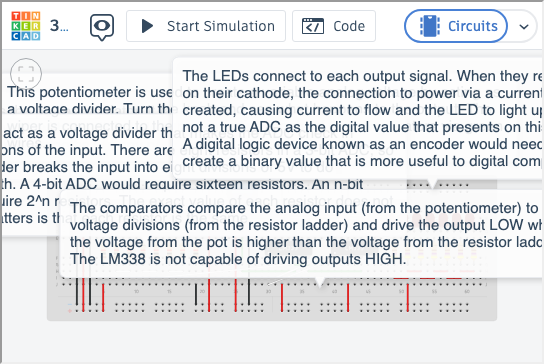
\includegraphics[width=\linewidth]{generated/preview/flashtypeadcontinkercad-2-preview.png}
\par
\end{sbspanel}%
\begin{sbspanel}{0.21}%
\par
\noindent
\includegraphics[width=\linewidth]{generated/qrcode/flashtypeadcontinkercad-2.png}
\par
\noindent{}\href{flashtypeadcontinkercad-2.html}{Standalone}%
\end{sbspanel}%
\end{sidebyside}%
\tcblower
\end{figureptx}%
\end{remark}
\end{subsectionptx}
%
%
\typeout{************************************************}
\typeout{Subsection 4.3.4 Pulse-Width Modulation (PWM)}
\typeout{************************************************}
%
\begin{subsectionptx}{Subsection}{Pulse-Width Modulation (PWM)}{}{Pulse-Width Modulation (PWM)}{}{}{ch4-pwm}
Pulse-width modulation (PWM) is a means of changing the average voltage of a signal without changing the minimum or maximum voltage levels that are used. In this manner, a digital electronic system (which, as mentioned, only uses two voltage levels) can vary the amount of time the signal is HIGH with respect to the amount of time the signal is LOW to modify the average voltage of the signal. PWM isn't just used in digital electronics. It is also an effective way of decreasing the average power supplied to a load while delivering a large maximum power by sending short pulses instead of a continuous signal. (This method is used in laser optics when a continuous laser beam would burn a hole in a sample, but repeated short pulses will not.) In addition, there are devices that specifically require a PWM signal to function properly (such as some servomotors).%
\par
PWM signals have multiple properties. The \ptxterminology{frequency} of the pulses corresponds to the number of pulses sent per unit of time. The concept of frequency was introduced in \hyperref[ch1-acsources]{Subsection~{\xreffont\ref{ch1-acsources}}}. \hyperref[ch1-periodfrequency]{({\xreffont\ref{ch1-periodfrequency}})} was used to relate the frequency and period of a periodic waveform. That same equation applies to a PWM waveform.%
\par
The \ptxterminology{duty cycle} of a PWM signal corresponds to the amount of time the signal is HIGH (\(T_{HIGH}\)) divided by the period of the waveform (\(T\)). This is essentially describing the fraction of time that the signal is HIGH every cycle. The equation for duty cycle (\(D\)) is defined in \hyperref[ch4-eqdutycycle]{({\xreffont\ref{ch4-eqdutycycle}})}, where \(T_{HIGH}\) is the amount of time the waveform is held HIGH every cycle and \(T_{LOW}\) is the amount of time the waveform is held LOW every cycle. (The period of the wave is therefore equal to \(T_{HIGH}+T_{LOW}\).)%
\par
%
\begin{equation}
D = \frac{T_{HIGH}}{T_{HIGH}+T_{LOW}}\label{ch4-eqdutycycle}
\end{equation}
%
\par
The \ptxterminology{average voltage} describes the mean voltage over the period of the wave. The equation for the average voltage (\(\bar{V}\)) of a PWM signal is described in \hyperref[ch4-eqavgvoltage]{({\xreffont\ref{ch4-eqavgvoltage}})}, where \(D\) is the duty cycle, \(V_{MAX}\) is the maximum value of the modulated signal, and \(V_{MIN}\) is the minimum value of the modulated signal.%
\par
%
\begin{equation}
\bar{V} = DV_{MAX} + (1-D)V_{MIN}\label{ch4-eqavgvoltage}
\end{equation}
%
\par
While PWM is accomplished using a completely different mechanism in digital electronics such as microcontrollers, it is possible to create a PWM circuit using a comparator, as shown in \hyperref[pwmcktfig]{Figure~{\xreffont\ref{pwmcktfig}}}. The input voltage (\(V_{IN}\)) can be a sinusoid or triangle wave. The reference voltage (\(V_{REF}\)) can be tuned to change the duty cycle of the output voltage (\(V_{OUT}\)). The output will saturate between \(V^-\) and \(V^+\).%
\begin{figureptx}{Figure}{Circuit schematic of a comparator used to generate a PWM signal.}{pwmcktfig}{}%
\begin{image}{0.3}{0.4}{0.3}{}%
\resizebox{\linewidth}{!}{%
\begin{tikzpicture}[font=\sffamily]
	\draw	(0,0) node[op amp] (opamp) {};
	\draw	(opamp.out) --++ (right:0.5) node[right] {$V_{OUT}$};
	\draw	(opamp.+) --++ (left:0.5) node[left] {$V_{REF}$};
	\draw	(opamp.-) --++ (left:0.5) node[left] {$V_{IN}$};
	\draw	(opamp.up)--++ (up:0.5) node[above] {$V^+$};
	\draw	(opamp.down) --++ (down:0.5) node[below] {$V^-$};
\end{tikzpicture}%
}%
\end{image}%
\tcblower
\end{figureptx}%
Example PWM waveforms given three different reference voltages \(V_{REF}\) with the same sinusoidal input signal \(V_{IN}\) are shown in \hyperref[pwmwavesfig]{Figure~{\xreffont\ref{pwmwavesfig}}}. As the reference voltage is increased, the duty cycle of the PWM waveform increases.%
\begin{figureptx}{Figure}{Three PWM signals (black waveform) with varying duty cycles. The input wave \(V_{IN}\) is represented by a red curve and the reference voltage \(V_{REF}\) is represented by a blue line.}{pwmwavesfig}{}%
\begin{image}{0}{1}{0}{}%
\resizebox{\linewidth}{!}{%
\begin{tikzpicture}[font=\sffamily]
	\begin{groupplot}[group style={group name=my plots, group size=1 by 3, vertical sep=0pt, xlabels at=edge bottom, xticklabels at=edge bottom,}, width=\linewidth, height=5cm, xlabel=$t$~(arbitrary), xmin=0, xmax=10, ticks=none]
	\nextgroupplot[ymin=-14, ymax=14, ylabel=$D\approx 20\%$]
		\addplot[red, samples=200, domain=0:10] {12*sin(deg(2*x)/2*pi)};
		\addplot[blue] coordinates {(0,-10) (10,-10)};
		\addplot[thick] coordinates {(0,-12) (1.31,-12) (1.31,12) (1.7,12) (1.7, -12) (3.31,-12) (3.31,12) (3.7,12) (3.7, -12) (5.31,-12) (5.31,12) (5.7,12) (5.7, -12) (7.31,-12) (7.31,12) (7.7,12) (7.7, -12) (9.31,-12) (9.31,12) (9.7,12) (9.7, -12) (10,-12)};
	\nextgroupplot[ymin=-14, ymax=14, ylabel=$D\approx 50\%$]
		\addplot[red, samples=200, domain=0:10] {12*sin(deg(2*x)/2*pi)};
		\addplot[blue] coordinates {(0,0) (10,0)};
		\addplot[thick] coordinates {(0,-12) (1,-12) (1,12) (2,12) (2,-12) (3,-12) (3,12) (4,12) (4,-12) (5,-12) (5,12) (6,12) (6,-12) (7,-12) (7,12) (8,12) (8,-12) (9,-12) (9,12) (10,12)};
	\nextgroupplot[ymin=-14, ymax=14, ylabel=$D\approx 80\%$]
		\addplot[red, samples=200, domain=0:10] {12*sin(deg(2*x)/2*pi)};
		\addplot[blue] coordinates {(0,10) (10,10)};
		\addplot[thick] coordinates {(0,12) (0.31,12) (0.31,-12) (0.69,-12) (0.69,12) (2.31,12) (2.31,-12) (2.69,-12) (2.69,12) (4.31,12) (4.31,-12) (4.69,-12) (4.69,12) (6.31,12) (6.31,-12) (6.69,-12) (6.69,12) (8.31,12) (8.31,-12) (8.69,-12) (8.69,12) (10,12)};
	\end{groupplot}
\end{tikzpicture}%
}%
\end{image}%
\tcblower
\end{figureptx}%
In this example, the frequency of the PWM waveform is set by the frequency of \(V_{IN}\). This makes a flexible PWM circuit where the minimum and maximum voltage values of the output are set by the comparator supply pins (\(V^+\) and \(V^-\)), the frequency is set by the input waveform, and the duty cycle is set by the reference voltage.%
\begin{remark}{Remark}{}{ch4-pwm-13}%
Play around with a simulation of a pulse-width modulation circuit in \hyperref[pwmcircuittinkercad]{Figure~{\xreffont\ref{pwmcircuittinkercad}}}. (To access this simulation in a new tab, use this link: \href{https://www.tinkercad.com/things/0G4jvHX5J7g}{\nolinkurl{Pulse-width modulation circuit}}.)%
\begin{figureptx}{Figure}{Pulse-width modulation circuit (TinkerCAD)}{pwmcircuittinkercad}{}%
\begin{sidebyside}{2}{0.075}{0.075}{0.17}%
\begin{sbspanel}{0.47}%
\par
\noindent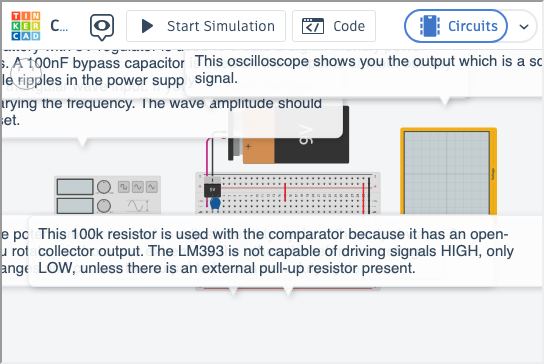
\includegraphics[width=\linewidth]{generated/preview/pwmcircuittinkercad-2-preview.png}
\par
\end{sbspanel}%
\begin{sbspanel}{0.21}%
\par
\noindent
\includegraphics[width=\linewidth]{generated/qrcode/pwmcircuittinkercad-2.png}
\par
\noindent{}\href{pwmcircuittinkercad-2.html}{Standalone}%
\end{sbspanel}%
\end{sidebyside}%
\tcblower
\end{figureptx}%
\end{remark}
\end{subsectionptx}
\end{sectionptx}
%
%
\typeout{************************************************}
\typeout{Section 4.4 Feedback Circuits}
\typeout{************************************************}
%
\begin{sectionptx}{Section}{Feedback Circuits}{}{Feedback Circuits}{}{}{ch4-feedback}
\begin{introduction}{}%
Feedback is a mechanism used to regulate, or control, the output of an electronic device.  Feedback systems have values or variables that affect each other. In closed-loop feedback, the variables or values affect each other directly (no intermediary is required to make changes). Closed-loop feedback operates with a \ptxterminology{setpoint} variable that describes the desired output of a system (e.g. the temperature of a room or the speed of a car), a \ptxterminology{process variable} that describes the current output value of the system, and an \ptxterminology{output} that affects the process variable (e.g. the home furnace or gas control to the engine of a car).%
\par
There are two types of feedback: positive and negative. In a system with \ptxterminology{positive feedback}, an increase to the process variable causes a corresponding increase to the output, which causes the process variable to increase more, which causes the output to increase even more, and so on. Alternatively, a decrease to the process variable would generate a decrease to the output, and so on. Positive feedback is inherently unstable as the process variable either increases or decreases out of bounds without ever settling to the setpoint level. Without a physical limitations to this process, energy could theoretically be amplified infinitely. This is undesirable.%
\begin{example}{Example}{Positive feedback: speaker and microphone.}{ch4-feedback-2-3}%
Positive feedback occurs when a speaker and microphone come in close proximity to each other. As sound goes into the microphone, it emits from the speaker. When the speaker is close to the microphone, the microphone will pick up that sound emission from the speaker and amplify it, which gets picked up by the microphone, and so on, until a loud squeal is emitted when the maximum amplification setting (saturation) is reached.%
\par
In this scenario, the setpoint (desired volume setting of the speakers) cannot be maintained, as the output (change in speaker volume) continues to increase with corresponding increases to the process variable (current volume emitted by the speaker).%
\end{example}
In a system with \ptxterminology{negative feedback}, the difference between the setpoint and process variable is used to create a change in the system output. The term \ptxterminology{negative} in negative feedback is used because the difference operation implies subtraction (negative). This causes the output to become self-correcting until the output becomes equal to the setpoint value. Because it is self-correcting, negative feedback forms the basis for modern control systems. (More information on control systems and feedback is available in \hyperlink{pasqualemicrobook}{[{\xreffont 4.7.5}]}.)%
\begin{example}{Example}{Negative feedback: adaptive cruise control.}{ch4-feedback-2-5}%
Adaptive cruise control is an example of a negative feedback system. The setpoint (desired speed) is programmed by the driver. The speed of the car at any moment in time is equal to the process variable. If the speed of the car becomes less than the setpoint, the difference between the setpoint and process variable becomes greater than zero and the adaptive cruise control will increase the power sent to the car's engine to speed the car up to the setpoint.%
\par
If the speed of the car becomes greater than the setpoint, the difference between the two variables becomes less than zero and the adaptive cruise control will decrease the power sent to the car's engine or brake the car to slow the car down to the setpoint.%
\par
If the speed of the car is exactly equal to the setpoint, the difference between the two variables is zero and no change to the car's engine power will be made.%
\end{example}
Negative feedback is also used in op-amp circuits. Because the gain of an op-amp is so high, it is impractical on its own as an amplifier, due to the fact that it saturates so rapidly (which was a feature in comparator circuits, but a drawback otherwise). However, feedback from the output to the inverting input can be used to tame the gain to a value that has practical uses.%
\par
Note that the remaining circuit diagrams in this chapter will not necessarily explicitly show the voltage supply connections. In a real circuit, supply connections must exist to power the op-amps. They are merely hidden in these diagrams to make them easier to read.%
\end{introduction}%
%
%
\typeout{************************************************}
\typeout{Subsection 4.4.1 Voltage Follower}
\typeout{************************************************}
%
\begin{subsectionptx}{Subsection}{Voltage Follower}{}{Voltage Follower}{}{}{ch4-voltagefollower}
A voltage follower circuit is the simplest type of negative feedback op-amp circuit. The output is fed into the inverting input, creating the relationship described in \hyperref[ch4-negfeedbackeq]{({\xreffont\ref{ch4-negfeedbackeq}})}.%
\par
%
\begin{equation}
V_{OUT} = A(V_P-V_{OUT})\label{ch4-negfeedbackeq}
\end{equation}
%
\par
The schematic of a voltage follower is shown in \hyperref[voltagefollowerfig]{Figure~{\xreffont\ref{voltagefollowerfig}}}.%
\begin{figureptx}{Figure}{Schematic of a voltage follower circuit.}{voltagefollowerfig}{}%
\begin{image}{0.25}{0.5}{0.25}{}%
\resizebox{\linewidth}{!}{%
\begin{tikzpicture}[font=\sffamily]
	\draw	(0,0) node[op amp] (opamp) {};
	\draw	(opamp.out) to [short, *-] ++ (right:0.75) node[right] {$V_{OUT}$};
	\draw	(opamp.+) --++ (left:0.5) node[left] {$V_{IN}$};
	\draw	(opamp.-)--++ (up:1) -| (opamp.out);
\end{tikzpicture}%
}%
\end{image}%
\tcblower
\end{figureptx}%
Assume that an input of 5~V is applied to \(V_{IN}\) while \(V_{OUT}\) is initially 0~V. The op-amp has a gain of 200,000. Plugging this information into \hyperref[ch4-negfeedbackeq]{({\xreffont\ref{ch4-negfeedbackeq}})}, the voltage difference of 5~V multiplied by 200,000 means that the output will attempt to increase dramatically.%
\par
Before the output can reach a value of one million, or even the positive supply voltage, however, it will increase slightly. (The rate at which the voltage levels increases is known as the \ptxterminology{slew rate}.) Let's say the output increases to 1~V. Now the voltage difference is only 4~V, and the output will try to drive to 4~V~\texttimes{}~200,000.%
\par
Before that happens, the voltage will increase a bit more, say, to 2~V. The voltage change now is only 3~V, so the output will not drive as high. At a certain point, the output will reach a stable level as close as possible to the input voltage of 5~V.%
\par
This circuit is called a voltage follower because the stability of the negative feedback system causes the output voltage to follow the input voltage. The gain of this circuit is one; the output equals the input without any multiplicative factor. What is the purpose of a circuit that does not change the value of the input voltage before passing it to the output? The purpose of a voltage follower is that the output follows the input while being effectively isolated from it. To understand what this means, consider \hyperref[ch4-voltagefollower9Vto5V]{Example~{\xreffont\ref{ch4-voltagefollower9Vto5V}}}.%
\begin{example}{Example}{Using a voltage follower to change the voltage of a battery.}{ch4-voltagefollower9Vto5V}%
Let's say that a 9~V battery needs to be used to create a stable output voltage of 5~V, over which a resistive load will be placed (but the exact resistance of the load is unknown and might be variable).%
\par
One way that a circuit designer could reduce a 9~V source to 5~V would be to create a voltage divider. This voltage divider is shown in \hyperref[voltagediv9to5]{Figure~{\xreffont\ref{voltagediv9to5}}}.%
\begin{figureptx}{Figure}{Voltage divider to convert a 9~V input into a 5~V output.}{voltagediv9to5}{}%
\begin{image}{0.3}{0.4}{0.3}{}%
\resizebox{\linewidth}{!}{%
\begin{tikzpicture}[font=\sffamily]
	\draw (0,2.5) to [battery1, l_=9~V] (0,0);
	\draw (0,2.5) to [R, l^=4~k$\Omega$] (2.5,2.5);
	\draw (2.5,2.5) to [R, l_=5~k$\Omega$, v^=$V_{OUT}$] (2.5,0);
	\draw (0,0) to [short] (2.5,0);	
\end{tikzpicture}%
}%
\end{image}%
\tcblower
\end{figureptx}%
Once a load is connected to the output of the voltage divider, however, the equivalent resistance of the voltage divider circuit changes. This is because the load would be in parallel with the 5~kΩ resistor, creating an equivalent resistance smaller than 5~kΩ.%
\par
The output voltage of the circuit will never be equal to the desired 5~V value unless the resistance of the load is infinite! The output voltage relationship, for this specific circuit, is described in \hyperref[voltagediv9to5eq]{({\xreffont\ref{voltagediv9to5eq}})}. Because the load resistance can be variable, it is not possible to engineer a voltage divider to account for the load resistance.%
\par
%
\begin{equation}
V_{OUT} = 9~\textrm{V} \left(\frac{5R_{LOAD}}{9R_{LOAD}+20}\right)\label{voltagediv9to5eq}
\end{equation}
%
\par
There needs to be another way to solve this problem. Fortunately, the voltage follower is the solution. Because of the negative feedback driving the output to be equal to the input, a load resistor will not affect the output voltage in any way. The circuit diagram for this solution is shown in \hyperref[voltagedivfollowerexamplefig]{Figure~{\xreffont\ref{voltagedivfollowerexamplefig}}}.%
\begin{figureptx}{Figure}{A voltage divider followed by a voltage follower will convert a 9~V input into a 5~V output regardless of the load resistance.}{voltagedivfollowerexamplefig}{}%
\begin{image}{0.1}{0.8}{0.1}{}%
\resizebox{\linewidth}{!}{%
\begin{tikzpicture}[font=\sffamily]
	\draw[]	(0,2.5) to [battery1, l_=9~V] (0,0);
	\draw[]	(0,2.5) to [R, l^=4~k$\Omega$] (2.5,2.5);
	\draw[]	(2.5,2.5) to [R, l_=5~k$\Omega$] (2.5,0);
	\draw[]	(0,0) to [short] (2.5,0);
	\draw[]	(3.5,2.5) node[op amp, anchor=+] (opamp) {};
	\draw[]	(opamp.+) to [short, -*] (2.5,2.5);
	\draw[]	(opamp.-) --++ (up:1) -| (opamp.out);
	\draw[]	(opamp.out) to [short, *-] ++(right:1);
	\draw[]	($(opamp.out)+(1,0)$) to [R, l_=$R_{LOAD}$, v^=5~V] ++(down:2.99);
	\draw[]	(2.5,0) to [short, *-] (6.885,0);
\end{tikzpicture}%
}%
\end{image}%
\tcblower
\end{figureptx}%
When connected as shown in \hyperref[voltagedivfollowerexamplefig]{Figure~{\xreffont\ref{voltagedivfollowerexamplefig}}}, there will be a 5~V drop over the load resistor. Ohm's law states that current will flow through the resistor. That current does not come from the battery, as the input resistance of an op-amp is very high (ideally infinite). Where does the current come from? It comes from the internal circuitry of the op-amp, which draws from the supply voltage. Remember: the op-amp is an active circuit element. (Refer to \hyperref[ch4-opampcurrent]{Section~{\xreffont\ref{ch4-opampcurrent}}} for more information on op-amp output current. The load resistor will be ultimately limited by the amount of current the op-amp can source.)%
\end{example}
\end{subsectionptx}
\end{sectionptx}
%
%
\typeout{************************************************}
\typeout{Section 4.5 Divided Feedback Op-Amp Circuits}
\typeout{************************************************}
%
\begin{sectionptx}{Section}{Divided Feedback Op-Amp Circuits}{}{Divided Feedback Op-Amp Circuits}{}{}{ch4-dividedfeedback}
\begin{introduction}{}%
The voltage follower has a gain of one. An op-amp without negative feedback has an extremely large gain. To exploit the shades of gray in between one and infinity, \ptxterminology{divided feedback} can be used. In divided feedback, the output is not directly connected to the input. There is now one or more resistor present in the feedback loop. A schematic of a generic divided feedback circuit is shown in \hyperref[dividedfeedbackfig]{Figure~{\xreffont\ref{dividedfeedbackfig}}}.%
\begin{figureptx}{Figure}{An op-amp connected with divided feedback.}{dividedfeedbackfig}{}%
\begin{image}{0.25}{0.5}{0.25}{}%
\resizebox{\linewidth}{!}{%
\begin{tikzpicture}[font=\sffamily]
	\draw[]	(3.5,1) node[op amp, scale=0.8] (opamp) {};
	\draw[]	(opamp.out) to [short] ($(opamp.out)+(1,0)$) node[right] {$V_{OUT}$};
	\draw[]	(opamp.+) node[left] {$V_P$};
	\draw[]	(opamp.-) to [short, *-] ($(opamp.-)+(0,0.75)$);
	\draw[]	($(opamp.-)-(2,0)$) node[left] {$V_1$} to [R, l^=$R_1$] (opamp.-) node[below] {$V_N$};
	\draw[]	($(opamp.-)+(0,0.75)$) to [R, l^=$R_2$] ($(opamp.-)+(2.5,0.75)$);
	\draw[]	($(opamp.-)+(2.5,0.75)$) to [short, -*] ($(opamp.-)+(2.5,-0.4)$);
\end{tikzpicture}%
}%
\end{image}%
\tcblower
\end{figureptx}%
Although the negative feedback path includes a resistor now (denoted as \(R_2\) in \hyperref[dividedfeedbackfig]{Figure~{\xreffont\ref{dividedfeedbackfig}}}), the same property that forced the output voltage of a voltage divider to be equal to the input voltage forces the voltage difference between the inverting and non-inverting inputs to be as close to zero as possible. The voltage at \(V_N\) will therefore be driven to be (ideally) exactly equal to \(V_P\). This is called a \ptxterminology{virtual node}; the two voltages are identical without being physically connected.%
\par
There are two very important properties of divided feedback op-amp circuits that come from the ideal op-amp characteristics (infinite gain, infinite input resistance, zero output resistance): \ptxalert{the voltage at both the inverting and non-inverting nodes is equal; and no current enters into either the inverting or non-inverting inputs of the op-amp.} These two properties will enable us to analyze all of the following op-amp circuits in this textbook.%
\par
Subsequent examples in this chapter will describe the gain of the op-amp circuit rather than the gain of the amplifier itself (which is considered to be infinitely high in an ideal op-amp). This circuit gain is defined in \hyperref[ch4-effectivegainopamp]{({\xreffont\ref{ch4-effectivegainopamp}})}. (Note that this is just a restatement of \hyperref[ch4-amplifiergainequation]{({\xreffont\ref{ch4-amplifiergainequation}})}.)%
\par
%
\begin{equation}
G = \frac{V_{OUT}}{V_{IN}}\label{ch4-effectivegainopamp}
\end{equation}
%
\begin{remark}{Remark}{Summary of circuit gain.}{ch4-dividedfeedback-2-7}%
%
\begin{itemize}[label=\ptxlistdisc]
\item{}Symbol: \(G\)%
\item{}Unit: none%
\end{itemize}
%
\end{remark}
\end{introduction}%
%
%
\typeout{************************************************}
\typeout{Subsection 4.5.1 Inverting Op-Amp}
\typeout{************************************************}
%
\begin{subsectionptx}{Subsection}{Inverting Op-Amp}{}{Inverting Op-Amp}{}{}{ch4-inverting}
An inverting op-amp circuit has a negative gain (defined by \hyperref[ch4-effectivegainopamp]{({\xreffont\ref{ch4-effectivegainopamp}})}). The output voltage is equal to the input voltage scaled by a negative number. The schematic of an inverting op-amp is shown in \hyperref[invertingopampfigure]{Figure~{\xreffont\ref{invertingopampfigure}}}.%
\begin{figureptx}{Figure}{Circuit diagram of an inverting op-amp.}{invertingopampfigure}{}%
\begin{image}{0.15}{0.7}{0.15}{}%
\resizebox{\linewidth}{!}{%
\begin{tikzpicture}[font=\sffamily]
	\draw	(3.5,1) node[op amp] (opamp) {};
	\draw[]	(opamp.out) to [short] ++ (right:0.5) node[right] {$V_{OUT}$};
	\draw[]	(opamp.+) node[ground] {};
	\draw[]	(opamp.-) to [short, *-] ($(opamp.-)+(0,0.75)$);
	\draw[]	($(opamp.-)-(2,0)$) to [V, l_=$V_{IN}$] ($(opamp.-)-(2,1.5)$) node[ground] {};
	\draw[]	($(opamp.-)-(2,0)$) to [R, l^=$R_1$] (opamp.-);
	\draw[]	($(opamp.-)+(0,0.75)$) to [R, l^=$R_2$] ($(opamp.-)+(2.38,0.75)$);
	\draw[]	($(opamp.-)+(2.38,0.75)$) to [short, -*] (opamp.out);
\end{tikzpicture}%
}%
\end{image}%
\tcblower
\end{figureptx}%
The basic design of an inverting op-amp requires two resistors (labeled \(R_1\) and \(R_2\) in \hyperref[invertingopampfigure]{Figure~{\xreffont\ref{invertingopampfigure}}}) to create divided feedback. The non-inverting input is connected to ground. Using the two properties of an ideal op-amp, the gain (\(G\)) of this circuit can be calculated.%
\par
First, KCL at the node where both resistors connect to the inverting input of the op-amp tells us that the current through resistor \(R_1\) must be equal to the current through resistor \(R_2\). This is true because no current enters into the op-amp through either the inverting or non-inverting inputs (this is one of the two important properties of divided feedback op-amp circuits).%
\par
Second, the voltages at each node in the circuit can be determined. The voltage at the inverting input node is equal to 0~V because of the virtual node with the non-inverting input, which is directly connected to ground. We can now use Ohm's law to calculate the gain of the circuit. The gain of an inverting op-amp circuit is defined in \hyperref[ch4-invertingopampgaineq]{({\xreffont\ref{ch4-invertingopampgaineq}})} and derived in \hyperlink{ch4-invertingopampgaineqproof}{Derivation~{\xreffont 4.5.1.1}}.%
\par
%
\begin{equation}
G = -\frac{R_2}{R_1}\label{ch4-invertingopampgaineq}
\end{equation}
%
\begin{proof}{Derivation}{}{ch4-invertingopampgaineqproof}
%
\begin{align*}
I_{R_1}	\amp= I_{R_2}\\
\frac{V_{IN}-0}{R_1} \amp= \frac{0-V_{OUT}}{R_2}\\
V_{OUT} 	\amp=	-\frac{R_2}{R_1}V_{IN}\\
G \amp= -\frac{R_2}{R_1}
\end{align*}
%
\end{proof}
The gain of an inverting op-amp circuit is therefore equal to \(-R_2/R_1\). Note that it is possible for an inverting op-amp to attenuate or amplify a signal. However, the output signal will always be inverted.%
\begin{example}{Example}{Inverting op-amp circuit.}{ch4-inverting-10}%
Calculate the gain and output voltage of the op-amp circuit shown in \hyperref[invertingopampexamplefig]{Figure~{\xreffont\ref{invertingopampexamplefig}}}. Assume that the supply pins are connected to a sufficiently high voltage not to saturate the output.%
\begin{figureptx}{Figure}{Inverting op-amp circuit.}{invertingopampexamplefig}{}%
\begin{image}{0.15}{0.7}{0.15}{}%
\resizebox{\linewidth}{!}{%
\begin{tikzpicture}[font=\sffamily]
	\draw	(3.5,1) node[op amp] (opamp) {};
	\draw[]	(opamp.out) to [short] ++ (right:0.5) node[right] {V\textsubscript{OUT}};
	\draw[]	(opamp.+) node[ground] {};
	\draw[]	(opamp.-) to [short, *-] ($(opamp.-)+(0,0.75)$);
	\draw[]	($(opamp.-)-(2,0)$) to [V, l_=0.5~V] ($(opamp.-)-(2,1.5)$) node[ground] {};
	\draw[]	($(opamp.-)-(2,0)$) to [R, l^=500~$\Omega$] (opamp.-);
	\draw[]	($(opamp.-)+(0,0.75)$) to [R, l^=2~k$\Omega$] ($(opamp.-)+(2.38,0.75)$);
	\draw[]	($(opamp.-)+(2.38,0.75)$) to [short, -*] (opamp.out);
\end{tikzpicture}%
}%
\end{image}%
\tcblower
\end{figureptx}%
This circuit is an inverting amplifier. The circuit gain is calculated below using \hyperref[ch4-invertingopampgaineq]{({\xreffont\ref{ch4-invertingopampgaineq}})}.%
\par
%
\begin{align*}
G \amp= \frac{-2000~\Omega}{500~\Omega}\\
\amp= -4
\end{align*}
%
\par
Multiply the input voltage by the gain to calculate the output voltage using \hyperref[ch4-amplifiergainequation]{({\xreffont\ref{ch4-amplifiergainequation}})}.%
\par
%
\begin{align*}
V_{OUT} \amp= (-4)(0.5~\textrm{V})\\
\amp= -2~\textrm{V}
\end{align*}
%
\end{example}
\end{subsectionptx}
%
%
\typeout{************************************************}
\typeout{Subsection 4.5.2 Non-Inverting Op-Amp}
\typeout{************************************************}
%
\begin{subsectionptx}{Subsection}{Non-Inverting Op-Amp}{}{Non-Inverting Op-Amp}{}{}{ch4-noninverting}
A non-inverting op-amp circuit has a positive gain; the output voltage is equal to the input voltage scaled by a positive number. The schematic for a non-inverting op-amp circuit is shown in \hyperref[noninvertingopampcktfigure]{Figure~{\xreffont\ref{noninvertingopampcktfigure}}}.%
\begin{figureptx}{Figure}{Circuit diagram of a non-inverting op-amp.}{noninvertingopampcktfigure}{}%
\begin{image}{0.2}{0.6}{0.2}{}%
\resizebox{\linewidth}{!}{%
\begin{tikzpicture}[font=\sffamily]
	\draw	(3.5,1) node[op amp] (opamp) {};
	\draw[]	(opamp.out) to [short] ++ (right:0.5) node[right] {$V_{OUT}$};
	\draw[]	(opamp.+) --++ (left:0.5);
	\draw[]	(opamp.-) to [short, *-] ($(opamp.-)+(0,0.75)$);
	\draw[]	($(opamp.+)-(0.5,0)$) to [V, l_=$V_{IN}$] ($(opamp.+)-(0.5,1.5)$) node[ground] {};
	\draw[]	($(opamp.-)-(2,0)$) node[ground] {} to [R, l^=$R_1$] (opamp.-);
	\draw[]	($(opamp.-)+(0,0.75)$) to [R, l^=$R_2$] ($(opamp.-)+(2.38,0.75)$);
	\draw[]	($(opamp.-)+(2.38,0.75)$) to [short, -*] (opamp.out);
\end{tikzpicture}%
}%
\end{image}%
\tcblower
\end{figureptx}%
The same two ideal op-amp properties will be used to determine the gain of this circuit. KCL at the inverting input node indicates that the current through resistor \(R_1\) is equal to the current through resistor \(R_2\) because no current enters into the op-amp itself. The voltage at the inverting input node is equal to \(V_{IN}\) due to the virtual node between inverting and non-inverting inputs. Ohm's law can be used to calculate the circuit properties, defined in \hyperref[ch4-noninvertingopampgaineq]{({\xreffont\ref{ch4-noninvertingopampgaineq}})} and derived in \hyperlink{ch4-noninvertingopampgaineqproof}{Derivation~{\xreffont 4.5.2.1}}.%
\par
%
\begin{equation}
G = 1+\frac{R_2}{R_1}\label{ch4-noninvertingopampgaineq}
\end{equation}
%
\begin{proof}{Derivation}{}{ch4-noninvertingopampgaineqproof}
%
\begin{align*}
I_{R_1}	\amp= I_{R_2}\\
\frac{0-V_{IN}}{R_1} \amp= \frac{V_{IN}-V_{OUT}}{R_2}\\
V_{OUT} 	\amp=	\left(1+\frac{R_2}{R_1}\right)V_{IN}\\
G \amp= 1+\frac{R_2}{R_1}
\end{align*}
%
\end{proof}
The gain of a non-inverting op-amp circuit is therefore equal to \(1+R_2/R_1\). Note that it is not possible for an inverting op-amp to attenuate a signal, only amplify it.%
\end{subsectionptx}
%
%
\typeout{************************************************}
\typeout{Subsection 4.5.3 Cascaded Op-Amps}
\typeout{************************************************}
%
\begin{subsectionptx}{Subsection}{Cascaded Op-Amps}{}{Cascaded Op-Amps}{}{}{ch4-cascaded}
It is possible to cascade op-amps; the output of one op-amp is fed into the input of a second op-amp, and so on. Each individual op-amp circuit is called a stage. \hyperref[cascadedblockfigure]{Figure~{\xreffont\ref{cascadedblockfigure}}} depicts a diagram of \(n\) cascaded op-amp circuits.%
\begin{figureptx}{Figure}{Block diagram of \(n\) cascaded op-amp circuits.}{cascadedblockfigure}{}%
\begin{image}{0}{1}{0}{}%
\resizebox{\linewidth}{!}{%
\begin{tikzpicture}[font=\sffamily]
	\foreach \x/\name/\num in {0/amp1/1, 2/amp2/2, 4/amp3/3, 6/amp4/4, 10/amp5/n} {
		\draw[]	(\x,0) node[ampshape] (\name) {};
		\node[right]	at (\name.west) {$G_\num$};
		\draw[]	($(\name.south west)-(0.25,0.25)$) rectangle ($(\name.north east)+(0.25,0.25)$);
	}
	\draw (amp1.left) --++ (left:1) node[left] {$V_{IN}$};
	\draw (amp1.right) -- (amp2.left);
	\draw (amp2.right) -- (amp3.left);
	\draw (amp3.right) -- (amp4.left);
	\draw (amp4.right) --++ (right:1);
	\node[align=center] at (8,0) {\large{...}};
	\draw (amp5.left) --++ (left:1);
	\draw (amp5.right) --++ (right:1) node[right] {$V_{OUT}$};
\end{tikzpicture}%
}%
\end{image}%
\tcblower
\end{figureptx}%
In general, assuming that saturation does not occur at any stage, \(n\) op-amps cascaded as shown in the \hyperref[cascadedblockfigure]{Figure~{\xreffont\ref{cascadedblockfigure}}}, with individual gains of \(GA_1\) through \(G_n\) will have a gain equal to the product of all of the individual gains, as expressed in \hyperref[ch4-cascadedtotaleq]{({\xreffont\ref{ch4-cascadedtotaleq}})}.%
\par
%
\begin{equation}
G_{TOTAL} = \prod_{i=1}^{n} G_{i}\label{ch4-cascadedtotaleq}
\end{equation}
%
\par
Cascading op-amps can be beneficial to increase overall circuit gain. Multiple stages can also be useful in active filter circuits (which will be discussed in \hyperref[ch9-activefilters]{Section~{\xreffont\ref{ch9-activefilters}}} in this book). Realistically, non-idealities in op-amps may cause compounding issues when op-amp circuits are cascaded together, as non-idealities in the early stages will be amplified by subsequent stages.%
\begin{example}{Example}{Cascaded op-amp circuit.}{ch4-cascaded-7}%
Calculate the total circuit gain of the op-amp circuit shown in \hyperref[cascadedinvertingexamplefig]{Figure~{\xreffont\ref{cascadedinvertingexamplefig}}}.%
\begin{figureptx}{Figure}{Two cascaded inverting op-amps.}{cascadedinvertingexamplefig}{}%
\begin{image}{0}{1}{0}{}%
\resizebox{\linewidth}{!}{%
\begin{tikzpicture}[font=\sffamily]
	\draw	(0,0) node[op amp] (opamp) {};
	\draw[]	(opamp.+) node[ground] {};
	\draw[]	(opamp.-) node[below] {A} to [short, *-] ($(opamp.-)+(0,0.75)$);
	\draw	(3,0) node[op amp, anchor=-] (opamp2) {};
	\draw[]	(opamp2.out) to [short] ++(right:0.5) node[right] {$V_{OUT}$};
	\draw[]	(opamp2.+) node[ground] {};
	\draw[]	(opamp2.-) node[below] {C} to [short, *-] ($(opamp2.-)+(0,0.75)$);
	\draw[]	(opamp.out) node[below] {B} to [R, l^=$R_3$] (opamp2.-);
	\draw[]	($(opamp2.-)+(0,0.75)$) to [R, l^=$R_4$] ($(opamp2.-)+(2.38,0.75)$);
	\draw[]	($(opamp2.-)+(2.38,0.75)$) to [short, -*] (opamp2.out);
	\draw[]	($(opamp.-)-(2,0)$) to [V, l_=$V_{IN}$] ($(opamp.-)-(2,1.25)$) node[ground] {};
	\draw[]	($(opamp.-)-(2,0)$) to [R, l^=$R_1$] (opamp.-);
	\draw[]	($(opamp.-)+(0,0.75)$) to [R, l^=$R_2$] ($(opamp.-)+(2.38,0.75)$);
	\draw[]	($(opamp.-)+(2.38,0.75)$) to [short, -*] (opamp.out);
\end{tikzpicture}%
}%
\end{image}%
\tcblower
\end{figureptx}%
It is possible to analyze this circuit by using the ideal op-amp properties. The current through \(R_1\) is equal to the current through \(R_2\). In addition, the voltage at node A is equal to the voltage at the non-inverting node of that op-amp, which is zero. This information can be used to calculate the voltage at node B. (This derivation was shown in \hyperlink{ch4-invertingopampgaineqproof}{Derivation~{\xreffont 4.5.1.1}}.)%
\par
%
\begin{equation*}
V_B = -\frac{R_2}{R_1}V_{IN}
\end{equation*}
%
\par
The current through \(R_3\) is equal to the current through \(R_4\). (The current through \(R_2\) is \ptxalert{not} necessarily equal to the current through \(R_3\), however!) Additionally, the voltage at node C is equal to 0~V due to the virtual node with the non-inverting input.%
\par
%
\begin{equation*}
V_{OUT} = -\frac{R_4}{R_3}V_B
\end{equation*}
%
\par
Using the previous calculation of \(V_B\), the overall circuit gain can be calculated.%
\par
%
\begin{align*}
V_{OUT} \amp= -\frac{R_4}{R_3}(-\frac{R_2}{R_1}V_{IN})\\
G \amp= \frac{R_4}{R_3}\frac{R_2}{R_1}
\end{align*}
%
\par
Alternatively, by inspecting the circuit diagram, it's clear that both op-amps are inverting op-amps. The individual gain of each op-amp can be multiplied together to calculate the overall circuit gain.%
\par
%
\begin{align*}
G \amp= G_1 G_2\\
\amp= (-\frac{R_2}{R_1})(-\frac{R_4}{R_3})\\
\amp=\frac{R_4}{R_3}\frac{R_2}{R_1}
\end{align*}
%
\end{example}
\end{subsectionptx}
%
%
\typeout{************************************************}
\typeout{Subsection 4.5.4 Summing and Difference Amplifiers}
\typeout{************************************************}
%
\begin{subsectionptx}{Subsection}{Summing and Difference Amplifiers}{}{Summing and Difference Amplifiers}{}{}{ch4-summingdifference}
A summing amplifier has an output proportional to the sum of multiple voltage sources. A schematic of a summing op-amp circuit is shown in \hyperref[summingampfigure]{Figure~{\xreffont\ref{summingampfigure}}}.%
\begin{figureptx}{Figure}{Circuit diagram of a summing amplifier.}{summingampfigure}{}%
\begin{image}{0.1}{0.8}{0.1}{}%
\resizebox{\linewidth}{!}{%
\begin{tikzpicture}[font=\sffamily]
	\draw	(3.5,1) node[op amp] (opamp) {};
	\draw[]	(opamp.out) to [short] ++ (right:0.5) node[right] {$V_{OUT}$};
	\draw[]	(opamp.-) to [short, *-] ($(opamp.-)+(0,0.75)$);
	\draw[]	(opamp.+) node[ground] {};
	\draw[]	(opamp.-) to [short, -*] ++(left:0.5);
	\draw[]	($(opamp.-)-(0.5,1)$) --++ (up:2);
	\draw[]	($(opamp.-)-(2.5,1)$) to [R, l^=$R_3$] ($(opamp.-)-(0.5,1)$);
	\draw[]	($(opamp.-)-(2.5,1)$) to [V, l_=$V_3$] ($(opamp.+)-(2.5,2)$) node[ground] {};
	\draw[]	($(opamp.-)-(3.5,0)$) to [R, l^=$R_2$] ($(opamp.-)-(0.5,0)$);
	\draw[]	($(opamp.-)-(3.5,0)$) to [V, l_=$V_2$] ($(opamp.+)-(3.5,1)$) node[ground] {};
	\draw[]	($(opamp.-)-(4.5,-1)$) to [R, l^=$R_1$] ($(opamp.-)-(0.5,-1)$);
	\draw[]	($(opamp.-)-(4.5,-1)$) to [V, l_=$V_1$] ($(opamp.+)-(4.5,0)$) node[ground] {};
	\draw[]	($(opamp.-)+(0,0.75)$) to [R, l^=$R_F$] ($(opamp.-)+(2.38,0.75)$);
	\draw[]	($(opamp.-)+(2.38,0.75)$) to [short, -*] (opamp.out);
\end{tikzpicture}%
}%
\end{image}%
\tcblower
\end{figureptx}%
Using KCL at the inverting input and Ohm's law, it is possible to derive the output equation of the op-amp circuit, given in \hyperref[ch4-invertingsummingampeq]{({\xreffont\ref{ch4-invertingsummingampeq}})}.%
\par
%
\begin{equation}
V_{OUT} = -R_F\left(\frac{V_1}{R_1}+\frac{V_2}{R_2}+\frac{V_3}{R_3}\right)\label{ch4-invertingsummingampeq}
\end{equation}
%
\par
It's no longer relevant to discuss the overall circuit gain, as each individual source has its own gain applied to it by the circuit (as opposed to a single source being modified by one overall circuit gain). These source gains can be determined by analyzing the proportionality constant applied to each source in the absence of all other sources. (In other words, the gain applied to source \(V_1\) is equal to the output voltage divided by \(V_1\) with \(V_2\) and \(V_3\) set equal to zero.) The input gains of this circuit are listed in \hyperref[ch4-summing-v1gain]{({\xreffont\ref{ch4-summing-v1gain}})}, \hyperref[ch4-summing-v2gain]{({\xreffont\ref{ch4-summing-v2gain}})}, and \hyperref[ch4-summing-v3gain]{({\xreffont\ref{ch4-summing-v3gain}})}.%
\par
%
\begin{align}
G_1 \amp= -\frac{R_F}{R_1}\label{ch4-summing-v1gain}\\
G_2 \amp= -\frac{R_F}{R_2}\label{ch4-summing-v2gain}\\
G_3 \amp= -\frac{R_F}{R_3}\label{ch4-summing-v3gain}
\end{align}
%
\par
Note that the inverting configuration of this op-amp circuit means that each individual source gain is negative. If it's necessary to have a non-inverting summing amplifier, either a non-inverting op-amp circuit can be used (as demonstrated in \hyperref[ch4-summingnoninvertingopamp]{Example~{\xreffont\ref{ch4-summingnoninvertingopamp}}}), or the inverting summing amplifier can be cascaded into an additional inverting amplifier, creating a two-stage circuit.%
\begin{example}{Example}{Non-inverting summing op-amp circuit.}{ch4-summingnoninvertingopamp}%
Calculate the output voltage of the op-amp circuit shown in \hyperref[noninvertingsummingopampcircuitdiagram]{Figure~{\xreffont\ref{noninvertingsummingopampcircuitdiagram}}}.%
\begin{figureptx}{Figure}{Non-inverting summing op-amp circuit.}{noninvertingsummingopampcircuitdiagram}{}%
\begin{image}{0.2}{0.6}{0.2}{}%
\resizebox{\linewidth}{!}{%
\begin{tikzpicture}[font=\sffamily]
	\draw[]	(3.5,1) node[op amp] (opamp) {};
	\draw[]	(opamp.out) to [short] ++ (right:0.5) node[right] {$V_{OUT}$};
	\draw[]	(opamp.-) to [short, *-] ($(opamp.-)+(0,0.75)$);
	\draw[]	(opamp.+) to [short]					++ (left:2.5);
	\draw[]	(opamp.-) to [R, l_=$R_I$]				++ (left:2.5) node[ground] {};
	\draw[]	($(opamp.+)-(1,0)$) to [R, l_=$R_2$, *-]	++ (down:2);
	\draw[]	($(opamp.+)-(1,2)$) to [V, l_=$V_2$]		++ (down:2) node[ground] {};
	\draw[]	($(opamp.+)-(2.5,0)$) to [R, l_=$R_1$]	++ (down:2);
	\draw[]	($(opamp.+)-(2.5,2)$) to [V, l_=$V_1$]	++ (down:2) node[ground] {};
	\draw[]	($(opamp.-)+(0,0.75)$) to [R, l^=$R_F$] ($(opamp.-)+(2.38,0.75)$);
	\draw[]	($(opamp.-)+(2.38,0.75)$) to [short, -*] (opamp.out);
\end{tikzpicture}%
}%
\end{image}%
\tcblower
\end{figureptx}%
Use KCL at the inverting node to calculate a relationship between that node voltage (which will be referred to as \(V_X\) in this example) and the output voltage.%
\par
%
\begin{align*}
\frac{0-V_X}{R_I} \amp= \frac{V_X-V_{OUT}}{R_F}\\
-\frac{V_X}{R_I}-\frac{V_X}{R_F} \amp= -\frac{V_{OUT}}{R_F}\\
\frac{R_FV_X + R_IV_X}{R_IR_F} \amp= \frac{V_{OUT}}{R_F}\\
(R_F+R_I)V_X \amp= R_I V_{OUT}\\
V_X \amp= V_{OUT}\left(\frac{R_I}{R_F+R_I}\right)
\end{align*}
%
\par
Use KCL at the non-inverting node to calculate a relationship between \(V_X\) and the two source voltages. (Recall that the voltage at the non-inverting node is equal to the voltage at the inverting node due to the virtual node property of an op-amp circuit).%
\par
%
\begin{align*}
\frac{V_1-V_X}{R_1} + \frac{V_2-V_X}{R_2} \amp= 0\\
\frac{R_2(V_1-V_X)}{R_1R_2} + \frac{R_1(V_2-V_X)}{R_1R_2} \amp= 0\\
R_2V_1 - R_2V_X + R_1V_2 - R_1V_X \amp= 0\\
R_2V_1 + R_1V_2 \amp= (R_1+R_2)V_X\\
V_1\left(\frac{R_2}{R_1+R_2}\right) + V_2\left(\frac{R_1}{R_1+R_2}\right) \amp= V_X\\
V_1\left(\frac{R_2}{R_1+R_2}\right) + V_2\left(\frac{R_1}{R_1+R_2}\right) \amp= V_{OUT}\left(\frac{R_I}{R_F+R_I}\right)\\
V_1\left(\frac{R_F+R_I}{R_I}\right)\left(\frac{R_2}{R_1+R_2}\right) + V_2\left(\frac{R_F+R_I}{R_I}\right)\left(\frac{R_1}{R_1+R_2}\right) \amp= V_{OUT}
\end{align*}
%
\par
The circuit gain of each source is listed below.%
\par
%
\begin{align*}
G_1 \amp= \left(\frac{R_F+R_I}{R_I}\right)\left(\frac{R_2}{R_1+R_2}\right)\\
G_2 \amp= \left(\frac{R_F+R_I}{R_I}\right)\left(\frac{R_1}{R_1+R_2}\right)
\end{align*}
%
\end{example}
The schematic for a difference amplifier is shown in \hyperref[differenceampcircuitdiagram]{Figure~{\xreffont\ref{differenceampcircuitdiagram}}}.%
\begin{figureptx}{Figure}{Circuit diagram of a difference amplifier.}{differenceampcircuitdiagram}{}%
\begin{image}{0.1}{0.8}{0.1}{}%
\resizebox{\linewidth}{!}{%
\begin{tikzpicture}[font=\sffamily]
	\draw[]	(3.5,1) node[op amp] (opamp) {};
	\draw[]	(opamp.out) to [short] ++ (right:0.5) node[right] {$V_{OUT}$};
	\draw[]	(opamp.-) to [short, *-] ($(opamp.-)+(0,0.75)$);
	\draw[]	($(opamp.+)-(2,0)$) to [R, l^=$R_2$] (opamp.+);
	\draw[]	($(opamp.+)-(2,0)$) to [V, l_=$V_2$] ($(opamp.+)-(2,1.5)$) node[ground] {};
	\draw[]	($(opamp.-)-(3.5,0)$) to [R, l^=$R_1$] (opamp.-);
	\draw[]	($(opamp.-)-(3.5,0)$) to [V, l_=$V_1$] ($(opamp.+)-(3.5,1)$) node[ground] {};
	\draw[]	(opamp.+) to [R, l_=$R_I$, *-] ($(opamp.+)-(0,2)$) node[ground] {};
	\draw[]	($(opamp.-)+(0,0.75)$) to [R, l^=$R_F$] ($(opamp.-)+(2.38,0.75)$);
	\draw[]	($(opamp.-)+(2.38,0.75)$) to [short, -*] (opamp.out);
\end{tikzpicture}%
}%
\end{image}%
\tcblower
\end{figureptx}%
This circuit can be solved for \(V_{OUT}\) using a voltage divider to calculate the input at the non-inverting node, and then applying KCL to the inverting node. The output equation is shown in \hyperref[ch4-differenceopamp]{({\xreffont\ref{ch4-differenceopamp}})} and derived in \hyperlink{ch4-differenceopampproof}{Derivation~{\xreffont 4.5.4.1}}.%
\par
%
\begin{equation}
V_{OUT} = -\frac{R_F}{R_1}V_1 + \left(\frac{R_F+R_1}{R_1}\right)\left(\frac{R_I}{R_2+R_I}\right)V_2\label{ch4-differenceopamp}
\end{equation}
%
\begin{proof}{Derivation}{}{ch4-differenceopampproof}
Use a voltage divider at the non-inverting node to calculate the node voltage, which will be called \(V_X\).%
\par
%
\begin{equation*}
V_X = \left(\frac{R_I}{R_2+R_I}\right)V_2
\end{equation*}
%
\par
Use KCL at the inverting node to calculate the output voltage.%
\par
%
\begin{align*}
\frac{V_1-V_X}{R_1} \amp= \frac{V_X-V_{OUT}}{R_F}\\
\frac{V_1}{R_1} - \frac{V_X}{R_1} - \frac{V_X}{R_F} \amp= -\frac{V_{OUT}}{R_F}\\
\frac{V_1}{R_1} - \frac{(R_F+R_1)V_X}{R_1R_F} \amp= -\frac{V_{OUT}}{R_F}\\
\frac{V_1}{R_1} - \left(\frac{R_F+R_1}{R_1R_F}\right)\left(\frac{R_I}{R_2+R_I}\right) \amp= -\frac{V_{OUT}}{R_F}\\
-\left(\frac{R_F}{R_1}\right)V_1 + \left(\frac{R_F+R_1}{R_1}\right)\left(\frac{R_I}{R_2+R_I}\right)V_2 \amp= V_{OUT}
\end{align*}
%
\end{proof}
The input gains of this circuit are listed in \hyperref[ch4-difference-v1gain]{({\xreffont\ref{ch4-difference-v1gain}})} and \hyperref[ch4-difference-v2gain]{({\xreffont\ref{ch4-difference-v2gain}})}.%
\par
%
\begin{align}
G_1 \amp= -\frac{R_F}{R_1}\label{ch4-difference-v1gain}\\
G_2 \amp= \left(\frac{R_F+R_1}{R_1}\right)\left(\frac{R_I}{R_2+R_I}\right)\label{ch4-difference-v2gain}
\end{align}
%
\end{subsectionptx}
%
%
\typeout{************************************************}
\typeout{Subsection 4.5.5 General Op-Amp Circuits}
\typeout{************************************************}
%
\begin{subsectionptx}{Subsection}{General Op-Amp Circuits}{}{General Op-Amp Circuits}{}{}{ch4-generalopamps}
Not all op-amp circuits fall into the categories discussed above (inverting, non-inverting, summing, etc.). In those cases, careful analysis can lead to a mathematical understanding of the circuit properties. First: it must be emphasized that the op-amp properties (virtual node, no current entering the inputs) are only valid if there is negative feedback present in the circuit. In the absence of negative feedback, then those two assumptions cannot be used to solve for the circuit properties. However, if the presence of negative feedback is established, then circuit analysis tools can be used with the virtual node and zero-current input properties to solve for the circuit characteristics.%
\begin{example}{Example}{Current-sensing circuit.}{ch4-generalopamps-3}%
A photodiode is a circuit device that converts light to electric current. It is used as the input to an op-amp circuit, as shown in \hyperref[currentsensingcircuit]{Figure~{\xreffont\ref{currentsensingcircuit}}}. Calculate the output voltage and its relationship to \(I\), the current generated by the photodiode.%
\begin{figureptx}{Figure}{Current-sensing op-amp circuit.}{currentsensingcircuit}{}%
\begin{image}{0.25}{0.5}{0.25}{}%
\resizebox{\linewidth}{!}{%
\begin{tikzpicture}[font=\sffamily]
	\draw[]	(3.5,1) node[op amp] (opamp) {};
	\draw[]	(opamp.out) to [short] ++ (right:0.5) node[right] {$V_{OUT}$};
	\draw[]	(opamp.+) node[ground] {};
	\draw[]	(opamp.-) to [short, *-] ($(opamp.-)+(0,0.75)$);
	\draw[]	($(opamp.-)-(1.5,1.5)$) node[ground] {} to [pDo] ($(opamp.-)-(1.5,0)$);
	\draw[]	($(opamp.-)-(1.5,0)$) to [short, i^=$I$] (opamp.-);
	\draw[]	($(opamp.-)+(0,0.75)$) to [R, l^=$R$] ($(opamp.-)+(2.38,0.75)$);
	\draw[]	($(opamp.-)+(2.38,0.75)$) to [short, -*] (opamp.out);
\end{tikzpicture}%
}%
\end{image}%
\tcblower
\end{figureptx}%
First, it must be established that there is negative feedback included in this circuit. The presence of the resistor between the output voltage and the inverting input means that we can use the assumptions of an op-amp circuit to solve this.%
\par
The voltage at the inverting input must be equal to 0~V, as the non-inverting input is connected to ground. As no current can enter into the inverting input of the op-amp, the amount of current through the resistor must be equal to \(I\). Therefore a relationship between the output voltage and photodiode current can be derived.%
\par
%
\begin{equation*}
V_{OUT} = -IR
\end{equation*}
%
\end{example}
\begin{example}{Example}{T-network circuit.}{ch4-generalopamps-4}%
In order to generate a large value of circuit gain in an inverting amplifier, either the feedback resistor must be very large, the input resistor must be very small, or both. A T-network is used to generate a large circuit gain without this constraint on resistor values.%
\par
Calculate the output voltage and circuit gain of the T-network op-amp circuit shown in \hyperref[tnetworkcircuit]{Figure~{\xreffont\ref{tnetworkcircuit}}}.%
\begin{figureptx}{Figure}{T-network op-amp circuit.}{tnetworkcircuit}{}%
\begin{image}{0.15}{0.7}{0.15}{}%
\resizebox{\linewidth}{!}{%
\begin{tikzpicture}[font=\sffamily]
	\draw[]	(3.5,1) node[op amp] (opamp) {};
	\draw[]	(opamp.out) to [short] ++ (right:2.5) node[right] {$V_{OUT}$};
	\draw[]	(opamp.+) node[ground] {};
	\draw[]	(opamp.-) to [short, *-] ($(opamp.-)+(0,2.25)$);
	\draw[]	($(opamp.-)-(2,0)$) to [V, l_=0.1~V] ($(opamp.-)-(2,1.5)$) node[ground] {};
	\draw[]	($(opamp.-)-(2,0)$) to [R, l^=1~k$\Omega$] (opamp.-);
	\draw[]	($(opamp.-)+(0,2.25)$) to [R, l^=5~k$\Omega$] ($(opamp.-)+(2.38,2.25)$);
	\draw[]	($(opamp.-)+(2.38,2.25)$) to [R, l_=1~k$\Omega$, *-] ++(down:1.75) node[ground] {};
	\draw[]	($(opamp.-)+(2.38,2.25)$) to [R, l^=3~k$\Omega$] ($(opamp.-)+(4.38,2.25)$);
	\draw[]	($(opamp.-)+(4.38,2.25)$) to [short, -*] ($(opamp.out)+(2,0)$);
\end{tikzpicture}%
}%
\end{image}%
\tcblower
\end{figureptx}%
Because there is feedback between the output of the circuit and the inverting input, op-amp assumptions can be used to solve this circuit.%
\par
The voltage at the inverting input must be equal to 0~V. The current through the 1~kΩ input resistor can therefore be calculated.%
\par
%
\begin{align*}
I \amp= \frac{0.1~\textrm{V}}{1~\textrm{k}\Omega}\\
\amp= 0.1~\textrm{mA}
\end{align*}
%
\par
All of this current must flow through the 5~kΩ resistor (as no current can enter through the inverting input on the op-amp). The voltage at the T junction can be calculated using Ohm's law.%
\par
%
\begin{align*}
V_T \amp= -(0.1~\textrm{mA})(5~\textrm{k}\Omega)\\
\amp= -0.5~\textrm{V}
\end{align*}
%
\par
The current through the 1~kΩ resistor in the feedback network can now be calculated. Because the voltage at \(V_T\) is negative, we know that current must flow \textquotedblleft{}upward\textquotedblright{} through the resistor, and we will treat that as the positive direction.%
\par
%
\begin{align*}
I_{1k} \amp= \frac{0.5~\textrm{V}}{1~\textrm{k}\Omega}\\
\amp= 0.5~\textrm{mA}
\end{align*}
%
\par
Using KCL at the T junction, we can calculate that the current through the 3~kΩ resistor must be the sum of the two currents.%
\par
%
\begin{align*}
I_{3k} \amp= 0.5~\textrm{mA} + 0.1~\textrm{mA}\\
\amp= 0.6~\textrm{mA}
\end{align*}
%
\par
Now Ohm's law can be used to calculate the output voltage.%
\par
%
\begin{align*}
I \amp= \frac{V_T-V_{OUT}}{R} \\
\amp= \frac{-0.5~\textrm{V}-V_{OUT}}{3~\textrm{k}\Omega}\\
\amp= 0.6~\textrm{mA}\\
V_{OUT} \amp= -[(0.6~\textrm{mA})(3~\textrm{k}\Omega) + 0.5~\textrm{V}]\\
\amp= -2.3~\textrm{V}
\end{align*}
%
\par
The gain of this circuit is -23.%
\end{example}
\end{subsectionptx}
%
%
\typeout{************************************************}
\typeout{Subsection 4.5.6 Implementing Mathematical Functions with Op-Amps}
\typeout{************************************************}
%
\begin{subsectionptx}{Subsection}{Implementing Mathematical Functions with Op-Amps}{}{Implementing Mathematical Functions with Op-Amps}{}{}{ch4-math}
Op-amps can be used to implement many different mathematical functions. Addition and subtraction can be accomplished using summing and difference amplifiers, as discussed in \hyperref[ch4-summingdifference]{Subsection~{\xreffont\ref{ch4-summingdifference}}}. Simultaneous sets of addition and subtraction can be solved by using more than one op-amp, as discussed in \hyperref[ch4-linearequations]{Subsection~{\xreffont\ref{ch4-linearequations}}}.%
\par
Multiplication by a constant is accomplished by configuring an inverting (or non-inverting) amplifier circuit to have an amplifying gain. Division by a constant is accomplished by configuring an amplifier circuit to have an attenuating gain. (Note: it is very difficult computationally to multiply two variable values together. This is a constraint not limited to analog computation; it is also difficult in digital computers.)%
\par
Differentiation and integration can be implemented by using capacitors in the amplifier circuit, either in the feedback or input path. These two circuits will be discussed in \hyperref[ch5-differentiatorintegrator]{Section~{\xreffont\ref{ch5-differentiatorintegrator}}}.%
\par
While non-linear functions are outside the scope of this class, a diode has a natural logarithm response between voltage and current. Therefore a diode in an amplifier circuit can be used to implement either a \(\ln(x)\) or \(\textrm{e}^x\) response.%
\end{subsectionptx}
%
%
\typeout{************************************************}
\typeout{Subsection 4.5.7 Solving Linear Equations}
\typeout{************************************************}
%
\begin{subsectionptx}{Subsection}{Solving Linear Equations}{}{Solving Linear Equations}{}{}{ch4-linearequations}
It is possible to use op-amps to solve equations. In fact, op-amps were used in analog computers to perform calculations on many diverse physical quantities including ballistic projectile trajectory, aircraft stability and control, and even economic models. While a detailed history and explanation of analog computation is outside of the scope of this textbook, it makes for fascinating reading. (Refer to \hyperlink{analogcomputerkorn}{[{\xreffont 4.7.1}]}, \hyperlink{analogcomputerpeterson}{[{\xreffont 4.7.7}]}, \hyperlink{analogcomputerulmann}{[{\xreffont 4.7.9}]}, and \hyperlink{analogcomputerweyrick}{[{\xreffont 4.7.10}]}.)%
\par
This book will consider two scenarios of equation-solving. First, consider a single linear equation, shown in \hyperref[ch4-singlelineareq]{({\xreffont\ref{ch4-singlelineareq}})}.%
\par
%
\begin{equation}
a x + b = 0\label{ch4-singlelineareq}
\end{equation}
%
\par
An op-amp circuit can be used to solve this equation for \(x\). Consider the inverting op-amp shown in \hyperref[invertingopampfigure]{Figure~{\xreffont\ref{invertingopampfigure}}}. In this circuit, the coefficient \(a\) is the ratio of the feedback resistor to the input resistor: \(a = R_2/R_1\). The constant term \(b\) comes from the value of the voltage source: \(b = V_{IN}\). Finally, the output voltage contains the value of the variable \(x\).%
\par
Simultaneous linear equations can be solved by using more than one op-amp and using the features of a summing amplifier circuit. To solve two simultaneous linear equations (with output variables \(x\) and \(y\)), two op-amp stages are used to solve for each output variable. The first stage is an inverting summing amplifier with inputs proportional to \(x\), \(y\), and a constant. The output of this stage is either \(-x\) or \(-y\). The second stage is an inverting amplifier that solves for either \(x\) or \(y\). The circuit diagram of the two op-amp stages used to solve for \(-x\) and \(x\) is shown in \hyperref[twolinearequations]{Figure~{\xreffont\ref{twolinearequations}}}. The circuitry used to solve for \(-y\) and \(y\) is virtually identical.%
\begin{figureptx}{Figure}{Op-amp circuit that can solve two simultaneous linear equations. A virtually identical circuit that solves for \(-y\) and \(y\) is not shown.}{twolinearequations}{}%
\begin{image}{0}{1}{0}{}%
\resizebox{\linewidth}{!}{%
\begin{tikzpicture}[font=\sffamily]
	\draw[]	(0,0) node[op amp] (opamp) {};
	\node[ground]	at (opamp.+) {};
	\draw[]	($(opamp.-)+(-3.75,4)$) node[above] {V+} to [pR, name=b0, l_=$b_0$] ++ (down:1.5) node[below] {V--};
	\draw[]	($(opamp.-)+(-3.75,1)$) node[above] {$x$} to [pR, name=a0, l_=$a_0$] ++ (down:1.5) node[below] {$-x$};
	\draw[]	($(opamp.-)+(-3.75,-2)$) node[above] {$y$} to [pR, name=a1, l_=$a_1$] ++ (down:1.5) node[below] {$-y$};
	\draw[]	(opamp.out) node[below] {$-x$} to [R, *-] ++ (right:2);
	\draw[]	(opamp.-) to [short, -*] ++(left:0.5);
	\draw[]	($(opamp.-)+(-0.5,1)$) --++ (down:3);
	\draw[]	(a0.wiper) |- ($(opamp.-)-(2.5,1)$) to [R, -*] ($(opamp.-)-(0.5,1)$);
	\draw[]	($(opamp.-)-(2.5,0)$) node[left] {$x$} to [R] ($(opamp.-)-(0.5,0)$);
	\draw[]	(b0.wiper) -| ($(opamp.-)-(2.5,-1)$) to [R] ($(opamp.-)-(0.5,-1)$);
	\draw[]	(a1.wiper) -| ($(opamp.-)-(2.5,2)$) to [R] ($(opamp.-)-(0.5,2)$);
	\draw[]	(opamp.-) to [short, *-] ++(up:1.25) to [R] ++ (right:2.25) -| (opamp.out);
	\draw[]	($(opamp.out)+(2,0)$) node[op amp, anchor=-] (opamp2) {};
	\node[ground]	at (opamp2.+) {};
	\draw[]	(opamp2.-) to [short, *-] ++ (up:1.25) to [R] ++ (right:2.25) -| (opamp2.out);
	\draw[]	(opamp2.out) to [short, *-] ++(right:1) node[right] {$x$};
\end{tikzpicture}%
}%
\end{image}%
\tcblower
\end{figureptx}%
Scaling potentiometers are used to scale each output voltage to a coefficient before it is passed to an input resistor in the summing op-amp. Voltage supplies are used to generate the constant terms. This circuit can solve the equations shown in \hyperref[ch4-eqtwolineareqs1]{({\xreffont\ref{ch4-eqtwolineareqs1}})} and \hyperref[ch4-eqtwolineareqs2]{({\xreffont\ref{ch4-eqtwolineareqs2}})}. Equation \hyperref[ch4-eqtwolineareqs1]{({\xreffont\ref{ch4-eqtwolineareqs1}})} is derived in \hyperlink{ch4-simultaneousderivation}{Derivation~{\xreffont 4.5.7.1}}, which assumes that all resistors have an equal value of \(R\).%
\par
%
\begin{align}
0 \amp= a_1x+a_2y+b_0\label{ch4-eqtwolineareqs1}\\
0 \amp= a_3x+a_4y+b_1\label{ch4-eqtwolineareqs2}
\end{align}
%
\begin{proof}{Derivation}{}{ch4-simultaneousderivation}
%
\begin{align*}
\frac{b_0-0}{R} + \frac{x-0}{R} + \frac{a_0x-0}{R} + \frac{a_1y-0}{R} \amp= \frac{0-(-x)}{R}\\
b_0 + x + a_0x + a_1y \amp= x\\
b_0 + a_0x + a_1y \amp= 0
\end{align*}
%
\end{proof}
It must be noted that there are limitations with this circuit. There is a maximum and minimum value of voltage that can occur on the output, which is limited by the supply voltage. Therefore this equation-solving circuit cannot solve for arbitrarily large numbers. However, it can solve a scaled version of an equation. The output would then be multiplied by that scaling factor to obtain the correct output.%
\begin{remark}{Remark}{}{ch4-linearequations-12}%
Play around with a simulation of a linear equation solver on CircuitJS in \hyperref[circuitjslinearequationsolver]{Figure~{\xreffont\ref{circuitjslinearequationsolver}}}. You can change the values of each coefficient by moving the sliders on each potentiometer, labeled \(b_0\), \(b_1\), \(a_2\) and \(a_3\). (To access this simulation in a new tab, use this link: \href{https://www.falstad.com/circuit/circuitjs.html?ctz=DwYwlgTgBAZgvAIgIwKgFwM6IAwDpsEECsqYIiSeATAVQOx0DM2AHFQGwCcndqIARoiLZUAB0EIALI1QA3CENQBbTEICmAWiQoAfACgoUYAEMoADwqTJUJJypR6921VTwELZcYrDlYRFp8oAHMvZEICBAB6fUMTc0trRiJ7Rygkl1hEDyglUKRApT8EAJFgvPCRaIMjUwsEdIdWKElOdkbst2zc71LC-3zSkIoKqJia+PrktPYWZtbpjqzPHt9+wKGw8NHq4Gg6hsYaObbD0rdShU2tqti9xAakK2ObK1ccVEvKEZujO4RU5xpKbON4IC7Db5jXYTVIHKbpUHgq6Eba3CaPaxIOgnJzYxEfCHXKF-DE2KizQ5kxZggnIiI-aF1UksbBpews-FQT4VSrE9FPRiMHFpIWc7mQnYkgXYRL2ZiSMWElEMqXWWEpOgZc60r5EnaiNATLRIJxtY3ss4UZZXMQAexwuEkdGwzB5FRIUAwABtEAAlNQYMAYNDGAB2IDUqKMBqN2lxZrjDkkluQ1t1dod7CQLGy3r9AaDIfDkYZMbq5pFCZNzQimVTOXKtdE9rBjuEwjd4V4np9CH9geDYYjUeAZf61fmFaQ7BTKAbhIzrboWJZnYIc7zfYLg+LI7HxUTVCIVblNFBc+6NqgzYdRG4a8IG97-cLQ5LUP3Fck06gX45dYvRtShvVtkh4B9sCffMByLYcVX5TFyQcTUqUVOleUlBC0hlZC5RlNDdWVKEAHcYRQk1ZgBOx8QZUimSeFkXkQ6kMNiOiEipJibDxOtWKMdjkCeAFpQVXiRwE0l5S4wV2BokiyLwtUUIRMSGSCLChVmSSWFE7U1ImA4dKBexkxTPjgHU+i1SaUkqCoXT3n0-YpjsxIXOTOSdlkWNsRsastF86dOWI7UGzMWRhhHbzyyxNoaFmAK2jjYLQtycLIqc-oZz8+wtGyijPLYnykv86dWWS1T5JiwKTxsWTKp2ATErq39ASChqipiuwWq0brv3qvSqv6Pqfy-drBsa2Nq0YrQGLM8TYzm1qhNYQr+MW6yEti9o1uAJrbKaWbrEkf8Js6-onhO1k-3m2iDItNlmhYhb9hMhL5hO3b9onNoWjaVovoM4EBWBaiOvWuo-q4qH4sByH5g++YMTh-wkaQykCvBvaptNa6fzKlGDyS7K8qTW6hqJsncLJwnUns1kqK1RyKYrI8EyQtnCa0Dnj1apCAax-b+dqgWzoh8dTzxnFycmmLpdauKPMFo0PpOx6rGeu7XuaNXKRkrn5k0lrNMJn8jbN-DlaZE4cL1y2xex7XUg0dglKZmktf8V3qZdtUcy573yXeuL-at+541-NXYq5qPfI0NXYbD4oE8O+ZE4dgSDiOOF3fMgSodOZ4Tax0QJmSSimnLhxQ7cGQcjUd5PXIGkuQbj2PzL9GZigKuNdBOulDb0oMGbi4h5exAC+7qvi4ziYYcrjnVqxyyhA5nMe-R0UV872YNc3vfTuZ2WJe4s1vejpPfbP38L4G4-zuKO+e+68aH-FhA71NF+5RmQmv4WAfBYXNEwyUjhSbec9yy6yFOAhw9kY6UXsrfNUCCr6B2QdfS+UDT701-IxemXMCHJnwayUyIDqymVITWGWj8NCMSoakchScmEEGpipB2ZhYxTCINYbmbQiDdjcKJQMiA0FoDbvwcyXDoGcBsMIX8VBGDyLrsI1Aoj-iiQkYgYw0ijSSDitgIgiiGbLzUZ6Io4i27GBQAyGRF01ScD4doSiPBQQiMsVo6xLg7HcNZIwZcfNEh0AclIdRnjUDaIQMYGQviYoGOaOwXKJoyHsA9OYjRVjED8FsXyKyj11QER5BPQSsouJH3biff4ykTKG1ziUgutT-r30qWifJdMUKOCKRKR+HSmm4UJjDFCjSZbAEiOACA+ggA}{\nolinkurl{linear equation solver}}.)%
\begin{figureptx}{Figure}{Linear equation solver circuit (CircuitJS)}{circuitjslinearequationsolver}{}%
\begin{sidebyside}{2}{0.075}{0.075}{0.17}%
\begin{sbspanel}{0.47}%
\par
\noindent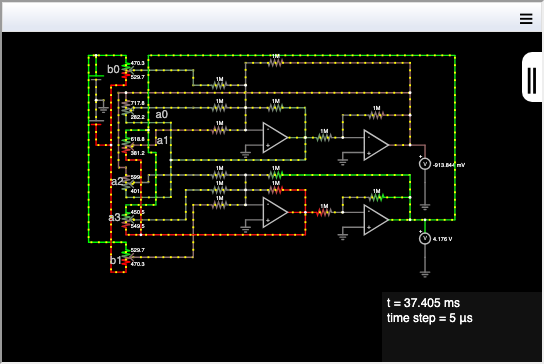
\includegraphics[width=\linewidth]{generated/preview/circuitjslinearequationsolver-2-preview.png}
\par
\end{sbspanel}%
\begin{sbspanel}{0.21}%
\par
\noindent
\includegraphics[width=\linewidth]{generated/qrcode/circuitjslinearequationsolver-2.png}
\par
\noindent{}\href{circuitjslinearequationsolver-2.html}{Standalone}%
\end{sbspanel}%
\end{sidebyside}%
\tcblower
\end{figureptx}%
Additionally, a non-simulated version of this circuit was built and described in \hyperlink{pasqualeanalogcomp}{[{\xreffont 4.7.6}]}.%
\end{remark}
It is also possible to solve differential equations using this method. This would require an op-amp building block that can take the integral of a voltage. Non-linear equations can be solved by designing op-amp building blocks that are capable of computing the desired function (say, using a diode to calculate natural logarithms).%
\end{subsectionptx}
\end{sectionptx}
%
%
\typeout{************************************************}
\typeout{Section 4.6 Op-Amp Output Current}
\typeout{************************************************}
%
\begin{sectionptx}{Section}{Op-Amp Output Current}{}{Op-Amp Output Current}{}{}{ch4-opampcurrent}
Up until this point, the discussion about op-amps has mostly been confined to discussions of voltages and voltage amplification. However, Ohm's law states that where there is voltage (and a closed path), there is current. Where does the current flowing through the load of an op-amp circuit come from? Consider the voltage follower shown in \hyperref[voltagefollowercurrentfigure]{Figure~{\xreffont\ref{voltagefollowercurrentfigure}}}.%
\begin{figureptx}{Figure}{A voltage follower circuit with current into and out of the op-amp labeled.}{voltagefollowercurrentfigure}{}%
\begin{image}{0.15}{0.7}{0.15}{}%
\resizebox{\linewidth}{!}{%
\begin{tikzpicture}[font=\sffamily]
	\draw[]	(0,2.5) to [V, l_=$V_{IN}$] (0,0);
	\draw[]	(0,2.5) to [R, l^=$R$] (2.5,2.5);
	\draw[]	(2.5,2.5) to [R, l_=$R$] (2.5,0);
	\draw[]	(0,0) to [short] (2.5,0);
	\draw[]	(3.5,2.5) node[op amp, anchor=+] (opamp) {};
	\draw[]	(2.5,2.5) to [short, *-, i_=0~mA] (opamp.+);
	\draw[]	($(opamp.-)-(0.5,0)$) to [short, i_=0~mA] (opamp.-);
	\draw[]	($(opamp.-)-(0.5,0)$) --++ (up:1) -| (opamp.out);
	\draw[]	(opamp.out) to [short, *-] ++(right:1);
	\draw[]	($(opamp.out)+(1,0)$) to [R, l_=$R_{LOAD}$, v^=$V_{OUT}$, i_=$I_{OUT}$] ++(down:2.99);
	\draw[]	(2.5,0) to [short, *-] (6.885,0);
\end{tikzpicture}%
}%
\end{image}%
\tcblower
\end{figureptx}%
In an ideal situation, no current flows into the inverting or non-inverting input terminals of an op-amp. This means that the feedback path of the voltage follower contributes no current to the load. Where does \(I_{OUT}\) come from? It must be sourced from the op-amp itself. The current comes from the power supply that's connected to the op-amp supply terminals, and then flows through the output of the op-amp into the load. This property of an integrated circuit to supply current is called \ptxterminology{sourcing current}. The op-amp of the voltage follower sources current. The amount of current that an op-amp can source is listed on the device datasheet.%
\par
In an inverting amplifier, the output current flows in the opposite direction, as shown in \hyperref[invertingopampcurrent]{Figure~{\xreffont\ref{invertingopampcurrent}}}.%
\begin{figureptx}{Figure}{Circuit diagram of an inverting op-amp with a resistive load, showing the direction of each current.}{invertingopampcurrent}{}%
\begin{image}{0.2}{0.6}{0.2}{}%
\resizebox{\linewidth}{!}{%
\begin{tikzpicture}[font=\sffamily]
	\draw[]	(3.5,1) node[op amp] (opamp) {};
	\draw[]	($(opamp.out)+(1,0)$) to [short, i_=$I_{SINK}$] (opamp.out);
	\draw[]	($(opamp.out)+(1,0)$) to [short] ++(down:0.25);
	\draw[]	($(opamp.out)+(1,-2.25)$) node[ground] {} to [R, l^=$R_{LOAD}$, v_=$V_{OUT}$, i^=$I_{OUT}$] ($(opamp.out)+(1,-0.25)$);
	\draw[]	(opamp.+) node[ground] {};
	\draw[]	(opamp.-) to [short, *-] ($(opamp.-)+(0,0.75)$);
	\draw[]	($(opamp.-)-(2,0)$) to [V, l_=$V_{IN}$] ($(opamp.-)-(2,1.5)$) node[ground] {};
	\draw[]	($(opamp.-)-(2,0)$) to [R, l^=$R_1$] (opamp.-);
	\draw[]	($(opamp.-)+(0,0.75)$) to [R, l^=$R_2$, i^=$I$] ($(opamp.-)+(3.38,0.75)$);
	\draw[]	($(opamp.-)+(3.38,0.75)$) to [short, -*] ($(opamp.out)+(1,0)$);
\end{tikzpicture}%
}%
\end{image}%
\tcblower
\end{figureptx}%
No current flows into the op-amp inputs. Now that the input voltage source is not electrically isolated from the output (as it was in the voltage follower circuit), the source is able to generate current. The op-amp will now have to accept current through its output node. This is known as \ptxterminology{sinking current}. The amount of current the op-amp must sink can be calculated by using KCL at the output node, shown in \hyperref[ch4-opampsinkcurrenteq]{({\xreffont\ref{ch4-opampsinkcurrenteq}})} and derived in \hyperlink{ch4-opampsinkderivation}{Derivation~{\xreffont 4.6.1}}. (Note that \(V_{OUT}\) is defined in the opposite direction as in \hyperref[ch4-inverting]{Subsection~{\xreffont\ref{ch4-inverting}}}, which is why the output voltage is expressed as a positive value in the derivation.)%
\par
%
\begin{equation}
I_{SINK} = \frac{V_{IN}}{R_1}\left(1+\frac{R_2}{R_{LOAD}}\right)\label{ch4-opampsinkcurrenteq}
\end{equation}
%
\begin{proof}{Derivation}{}{ch4-opampsinkderivation}
%
\begin{align*}
I_{SINK} \amp= I + I_{OUT}\\
\amp= \frac{V_{IN}}{R_1} + \frac{V_{OUT}}{R_{LOAD}}\\
\amp= \frac{V_{IN}}{R_1}+\frac{R_2V_{IN}}{R_1R_{LOAD}}\\
\amp= \frac{V_{IN}}{R_1}\left(1+\frac{R_2}{R_{LOAD}}\right)
\end{align*}
%
\end{proof}
The amount of current that an op-amp can sink is listed on the datasheet of the device. \hyperref[ch4-lm324datasheet]{Table~{\xreffont\ref{ch4-lm324datasheet}}} shows an example excerpt of the electrical characteristics section of the datasheet for the LM324 op-amp. It shows the minimum and typical values of output current that can be sourced or sunk under certain test settings. This particular op-amp is capable of sourcing much more current than it can sink. Paying attention to these characteristics is very important if particular current sourcing or sinking requirements must be met.%
\begin{tableptx}{Table}{\textbf{Example excerpt of the electrical characteristics section of the LM324 op-amp datasheet}}{ch4-lm324datasheet}{}%
\begin{tabularbox}{0}{1}{0}%
\resizebox{\ifdim\width > \linewidth\linewidth\else\width\fi}{!}{%
{\tabularfont%
\begin{tabular}{llllll}
\multicolumn{2}{m{0.2\linewidth}}{\raggedright%
Parameter%
}&\multicolumn{1}{m{0.5\linewidth}}{\raggedright%
Test Conditions%
}&\multicolumn{1}{m{0.1\linewidth}}{\raggedright%
Min%
}&\multicolumn{1}{m{0.1\linewidth}}{\raggedright%
Typ%
}&\multicolumn{1}{m{0.1\linewidth}}{\raggedright%
Unit%
}\tabularnewline\ptxhrulemedium
\multicolumn{1}{m{0.1\linewidth}}{\raggedright%
Output current%
}&\multicolumn{1}{m{0.1\linewidth}}{\raggedright%
Source%
}&\multicolumn{1}{m{0.5\linewidth}}{\raggedright%
\(V_{IN}^+ = 1~\textrm{V}\), \(V_{IN}^- = 0~\textrm{V}\), \(V^+ = 15~\textrm{V}\), \(V_o = 2~\textrm{V}\), \(T_A = 25^\circ\textrm{C}\)%
}&\multicolumn{1}{m{0.1\linewidth}}{\raggedright%
20%
}&\multicolumn{1}{m{0.1\linewidth}}{\raggedright%
40%
}&\multicolumn{1}{m{0.1\linewidth}}{\raggedright%
mA%
}\tabularnewline\ptxhrulethin
\multicolumn{1}{m{0.1\linewidth}}{\raggedright%
%
}&\multicolumn{1}{m{0.1\linewidth}}{\raggedright%
Sink%
}&\multicolumn{1}{m{0.5\linewidth}}{\raggedright%
\(V_{IN}^- = 1~\textrm{V}\), \(V_{IN}^+ = 0~\textrm{V}\), \(V^+ = 15~\textrm{V}\), \(V_o = 2~\textrm{V}\), \(T_A = 25^\circ\textrm{C}\)%
}&\multicolumn{1}{m{0.1\linewidth}}{\raggedright%
10%
}&\multicolumn{1}{m{0.1\linewidth}}{\raggedright%
20%
}&\multicolumn{1}{m{0.1\linewidth}}{\raggedright%
µA%
}\tabularnewline\ptxhrulethin
\multicolumn{1}{m{0.1\linewidth}}{\raggedright%
%
}&\multicolumn{1}{m{0.1\linewidth}}{\raggedright%
%
}&\multicolumn{1}{m{0.5\linewidth}}{\raggedright%
\(V_{IN}^- = 1~\textrm{V}\), \(V_{IN}^+ = 0~\textrm{V}\), \(V^+ = 15~\textrm{V}\), \(V_o = 200~\textrm{mV}\), \(T_A = 25^\circ\textrm{C}\)%
}&\multicolumn{1}{m{0.1\linewidth}}{\raggedright%
12%
}&\multicolumn{1}{m{0.1\linewidth}}{\raggedright%
50%
}&\multicolumn{1}{m{0.1\linewidth}}{\raggedright%
µA%
}\tabularnewline\ptxhrulethin
\end{tabular}
}%
}%
\end{tabularbox}%
\end{tableptx}%
Some datasheets list the output current specifications under a section labeled \ptxterminology{output short-circuit current} rather than \ptxterminology{output current} as shown in \hyperref[ch4-lm324datasheet]{Table~{\xreffont\ref{ch4-lm324datasheet}}}.%
\end{sectionptx}
%
%
\typeout{************************************************}
\typeout{References 4.7 References}
\typeout{************************************************}
%
\begin{references-section}{References}{References}{}{References}{}{}{opamp-references}
%% If this is a top-level references
%%   you can replace the "referencelist" environment
%%   with a standard "thebibliography" environment
\begin{referencelist}
\bibitem[1]{analogcomputerkorn}\hypertarget{analogcomputerkorn}{}Korn, G. A., and Korn, T. M. (1972). Electronic Analog and Hybrid Computers. McGraw-Hill Companies.
\bibitem[2]{ampsascomparators}\hypertarget{ampsascomparators}{}Moghimi, Reza. (2003, April). \textit{Ask The Applications Engineer\textemdash{}31: Amplifiers as Comparators?} \href{https://www.analog.com/en/analog-dialogue/articles/amplifiers-as-comparators.html}{https:\slash{}\slash{}www.analog.com\slash{}en\slash{}analog-dialogue\slash{}articles\slash{}amplifiers-as-comparators.html}
\bibitem[3]{howtoreadopampdatasheet}\hypertarget{howtoreadopampdatasheet}{}O'Donnell, Bill. \textit{How to Read an Op-Amp Data Sheet.} \href{www.physics.unlv.edu/\~bill/PHYS483/op_amp_datasheet.pdf}{www.physics.unlv.edu\slash{}\textasciitilde{}bill\slash{}PHYS483\slash{}op\textunderscore{}amp\textunderscore{}datasheet.pdf}
\bibitem[4]{pasqualedigitalbook}\hypertarget{pasqualedigitalbook}{}Pasquale, A. (2020). Digital Systems. \href{https://doctor-pasquale.com/wp-content/uploads/2020/11/DigitalSystemsBook.pdf}{https:\slash{}\slash{}doctor-pasquale.com\slash{}wp-content\slash{}uploads\slash{}2020\slash{}11\slash{}DigitalSystemsBook.pdf}
\bibitem[5]{pasqualemicrobook}\hypertarget{pasqualemicrobook}{}Pasquale, A. (2021). Microcontrollers. \href{https://doctor-pasquale.com/wp-content/uploads/2021/02/The-Yellow-Book.pdf}{https:\slash{}\slash{}doctor-pasquale.com\slash{}wp-content\slash{}uploads\slash{}2021\slash{}02\slash{}The-Yellow-Book.pdf}
\bibitem[6]{pasqualeanalogcomp}\hypertarget{pasqualeanalogcomp}{}Pasquale, A. (2024, September 17). Analog computation: solving simultaneous linear equations. \href{https://doctor-pasquale.com/2024/09/17/analog-computation-solving-simultaneous-linear-equations/}{https:\slash{}\slash{}doctor-pasquale.com\slash{}2024\slash{}09\slash{}17\slash{}analog-computation-solving-simultaneous-linear-equations\slash{}}
\bibitem[7]{analogcomputerpeterson}\hypertarget{analogcomputerpeterson}{}Peterson, G. R. (1971). Basic Analog Computation.‌
\bibitem[8]{understandingidealopamps}\hypertarget{understandingidealopamps}{}Texas Instruments. (1999, July). \textit{Understanding Basic Analog\textemdash{}Ideal Op Amps.} \href{https://www.ti.com/lit/an/slaa068b/slaa068b.pdf}{https:\slash{}\slash{}www.ti.com\slash{}lit\slash{}an\slash{}slaa068b\slash{}slaa068b.pdf}
\bibitem[9]{analogcomputerulmann}\hypertarget{analogcomputerulmann}{}Bernd Ulmann. (2022). Analog Computing. Walter de Gruyter GmbH and Co KG.
\bibitem[10]{analogcomputerweyrick}\hypertarget{analogcomputerweyrick}{}Weyrick, R. C. (1969). Fundamentals of Analog Computers. Prentice Hall.
\end{referencelist}
\end{references-section}
%
%
\typeout{************************************************}
\typeout{Exercises 4.8 Practice Problems}
\typeout{************************************************}
%
\begin{exercises-section}{Exercises}{Practice Problems}{}{Practice Problems}{}{}{ch4-op-amps-10}
\begin{introduction}{}%
For all questions, assume that the supply pins are connected to a suitable source that will not cause the output to saturate.%
\end{introduction}%
\paragraph{Divided Feedback Op-Amp Circuits}\hypertarget{ch4-op-amps-10-3}{}
\begin{divisionexercise}{1}{}{}{ch4dividedfeedbackex1}%
Calculate the output voltage and circuit gain of the circuit shown in \hyperref[examplecircuit41]{Figure~{\xreffont\ref{examplecircuit41}}}.%
\begin{figureptx}{Figure}{Circuit diagram corresponding to \hyperlink{ch4dividedfeedbackex1}{Exercise~{\xreffont 4.8.1}}.}{examplecircuit41}{}%
\begin{image}{0.2}{0.6}{0.2}{}%
\resizebox{\linewidth}{!}{%
\begin{tikzpicture}[font=\sffamily]
	\draw[]	(3.5,1) node[op amp] (opamp) {};
	\draw[]	(opamp.out) to [short] ++ (right:0.5) node[right] {$V_{OUT}$};
	\draw[]	(opamp.+) node[ground] {};
	\draw[]	(opamp.-) to [short, *-] ($(opamp.-)+(0,1.25)$);
	\draw[]	($(opamp.-)-(2,0)$) to [V, l_=0.5~V] ($(opamp.-)-(2,1.5)$) node[ground] {};
	\draw[]	($(opamp.-)-(2,0)$) to [R, l^=1~k$\Omega$] (opamp.-);
	\draw[]	($(opamp.-)+(0,1.25)$) to [R, l^=6~k$\Omega$] ($(opamp.-)+(2.38,1.25)$);
	\draw[]	($(opamp.-)+(2.38,1.25)$) to [short, -*] ($(opamp.out)+(0,0)$);		
\end{tikzpicture}%
}%
\end{image}%
\tcblower
\end{figureptx}%
\par\smallskip%
\noindent\textbf{\blocktitlefont Answer}.\hypertarget{ch4dividedfeedbackex1-2}{}\quad{}%
\begin{align*}
V_{OUT} \amp= -3~\textrm{V}\\
G \amp= -6
\end{align*}
%
\par\smallskip%
\noindent\textbf{\blocktitlefont Solution}.\hypertarget{ch4dividedfeedbackex1-3}{}\quad{}The circuit is an inverting op-amp circuit. Apply \hyperref[ch4-invertingopampgaineq]{({\xreffont\ref{ch4-invertingopampgaineq}})} to calculate the gain.%
\par
%
\begin{align*}
G \amp= -\frac{6~\textrm{k}\Omega}{1~\textrm{k}\Omega}\\
\amp= -6
\end{align*}
%
\par
Apply \hyperref[ch4-effectivegainopamp]{({\xreffont\ref{ch4-effectivegainopamp}})} to calculate the output voltage.%
\par
%
\begin{align*}
V_{OUT} \amp= GV_{IN}\\
\amp= (-6)(0.5~\textrm{V})\\
\amp= -3~\textrm{V}
\end{align*}
%
\end{divisionexercise}%
\begin{divisionexercise}{2}{}{}{ch4dividedfeedbackex2}%
Calculate the output voltage and circuit gain of the circuit shown in \hyperref[examplecircuit42]{Figure~{\xreffont\ref{examplecircuit42}}}.%
\begin{figureptx}{Figure}{Circuit diagram corresponding to \hyperlink{ch4dividedfeedbackex2}{Exercise~{\xreffont 4.8.2}}.}{examplecircuit42}{}%
\begin{image}{0.2}{0.6}{0.2}{}%
\resizebox{\linewidth}{!}{%
\begin{tikzpicture}[font=\sffamily]
	\draw[]	(3.5,1) node[op amp] (opamp) {};
	\draw[]	(opamp.out) to [short]						++ (right:0.5) node[right] {$V_{OUT}$};
	\draw[]	(opamp.+) to [short]							($(opamp.+)-(2,0)$);
	\draw[]	(opamp.+) to [R, l_=10~$\Omega$, *-]			++(down:2.5);
	\draw[]	($(opamp.+)-(2,2.5)$) to [I, l^=500~mA]			++(up:2.5);
	\draw[]	($(opamp.+)-(2,2.5)$) to [short]					++(right:2);
	\draw[]	(opamp.-) to [short, *-] 						($(opamp.-)+(0,1.25)$);
	\draw[]	(opamp.-) to [R, l_=50~k$\Omega$]				($(opamp.-)-(2,0)$) node[ground] {};
	\draw[]	($(opamp.-)+(0,1.25)$) to [R, l^=30~k$\Omega$]	($(opamp.-)+(2.38,1.25)$);
	\draw[]	($(opamp.-)+(2.38,1.25)$) to [short, -*]			($(opamp.out)+(0,0)$);		
\end{tikzpicture}%
}%
\end{image}%
\tcblower
\end{figureptx}%
\par\smallskip%
\noindent\textbf{\blocktitlefont Answer}.\hypertarget{ch4dividedfeedbackex2-2}{}\quad{}%
\begin{align*}
V_{OUT} \amp= 8~\textrm{V}\\
G \amp= 1.6
\end{align*}
%
\par\smallskip%
\noindent\textbf{\blocktitlefont Solution}.\hypertarget{ch4dividedfeedbackex2-3}{}\quad{}The circuit is a non-inverting op-amp circuit. Apply \hyperref[ch4-noninvertingopampgaineq]{({\xreffont\ref{ch4-noninvertingopampgaineq}})} to calculate the gain.%
\par
%
\begin{align*}
G \amp= 1 + \frac{30~\textrm{k}\Omega}{50~\textrm{k}\Omega}\\
\amp= 1.6
\end{align*}
%
\par
The voltage at the non-inverting node must be calculated before using \hyperref[ch4-effectivegainopamp]{({\xreffont\ref{ch4-effectivegainopamp}})} to calculate the output voltage. The voltage at the non-inverting node is equal to the voltage dropped over the 10~Ω resistor, which can be calculated with Ohm's law. (To obtain a unit of V, first convert the source current to A to multiply with Ω. Alternatively, convert the resistance to kΩ to multiply with mA.)%
\par
%
\begin{align*}
V_P \amp= (10~\Omega)(0.5~\textrm{A})\\
\amp= 5~\textrm{V}
\end{align*}
%
\par
Now use \hyperref[ch4-effectivegainopamp]{({\xreffont\ref{ch4-effectivegainopamp}})} to calculate the output voltage.%
\par
%
\begin{align*}
V_{OUT} \amp= GV_P\\
\amp= (1.6)(5~\textrm{V})\\
\amp= 8~\textrm{V}
\end{align*}
%
\end{divisionexercise}%
\begin{divisionexercise}{3}{}{}{ch4dividedfeedbackex3}%
Calculate the output voltage and source gains of the circuit shown in \hyperref[examplecircuit43]{Figure~{\xreffont\ref{examplecircuit43}}}.%
\begin{figureptx}{Figure}{Circuit diagram corresponding to \hyperlink{ch4dividedfeedbackex3}{Exercise~{\xreffont 4.8.3}}.}{examplecircuit43}{}%
\begin{image}{0.2}{0.6}{0.2}{}%
\resizebox{\linewidth}{!}{%
\begin{tikzpicture}[font=\sffamily]
	\draw[]	(3.5,1) node[op amp] (opamp) {};
	\draw[]	(opamp.out) to [short] ++ (right:0.5) node[right] {$V_{OUT}$};
	\draw[]	(opamp.+) node[ground] {};
	\draw[]	(opamp.-) to [short, *-] ($(opamp.-)+(0,1.25)$);
	\draw[]	($(opamp.-)-(2.5,0)$) to [V, l_={10~mV~(V1)}] ++(down:2) node[tlground] {};
	\draw[]	($(opamp.-)-(2.5,0)$) to [R, l^=2~k$\Omega$] ++(right:2);
	\draw[]	($(opamp.-)-(0.5,2)$) to [V, l_={300~mV~(V2)}] ++(down:1.5) node[tlground] {};
	\draw[]	($(opamp.-)-(0.5,0)$) to [R, l_=5~k$\Omega$, *-] ++(down:2);
	\draw[]	(opamp.-) to [short] ++(left:0.5);
	\draw[]	($(opamp.-)+(0,1.25)$) to [R, l^=10~k$\Omega$] ($(opamp.-)+(2.38,1.25)$);
	\draw[]	($(opamp.-)+(2.38,1.25)$) to [short, -*] ($(opamp.out)+(0,0)$);		
\end{tikzpicture}%
}%
\end{image}%
\tcblower
\end{figureptx}%
\par\smallskip%
\noindent\textbf{\blocktitlefont Answer}.\hypertarget{ch4dividedfeedbackex3-2}{}\quad{}%
\begin{align*}
V_{OUT} \amp= -0.65~\textrm{V}\\
G_1 \amp= -5\\
G_2 \amp= -2
\end{align*}
%
\par\smallskip%
\noindent\textbf{\blocktitlefont Solution}.\hypertarget{ch4dividedfeedbackex3-3}{}\quad{}The circuit is an inverting summing amplifier circuit. Apply \hyperref[ch4-invertingsummingampeq]{({\xreffont\ref{ch4-invertingsummingampeq}})} to calculate the output voltage and each of the source gains. The unit of each source has been converted to V.%
\par
%
\begin{align*}
V_{OUT} \amp= -\left(\frac{10~\textrm{k}\Omega}{2~\textrm{k}\Omega}\right)0.01~\textrm{V}-\left(\frac{10~\textrm{k}\Omega}{5~\textrm{k}\Omega}\right)0.3~\textrm{V}\\
\amp= -0.05~\textrm{V} - 0.6~\textrm{V}\\
\amp= -0.65~\textrm{V}\\
G_1 \amp= -\frac{10~\textrm{k}\Omega}{2~\textrm{k}\Omega}\\
\amp= -5\\
G_2 \amp= -\frac{10~\textrm{k}\Omega}{5~\textrm{k}\Omega}\\
\amp= -2
\end{align*}
%
\end{divisionexercise}%
\begin{divisionexercise}{4}{}{}{ch4dividedfeedbackex4}%
Calculate the circuit gain of the circuit shown in \hyperref[examplecircuit44]{Figure~{\xreffont\ref{examplecircuit44}}} as a function of \(x\). The potentiometer has a total resistance of 500~Ω. Calculate the minimum and maximum possible values of the circuit gain. Use the variable \(x\) to describe the potentiometer resistance between the wiper and 100~Ω resistor.%
\begin{figureptx}{Figure}{Circuit diagram corresponding to \hyperlink{ch4dividedfeedbackex4}{Exercise~{\xreffont 4.8.4}}.}{examplecircuit44}{}%
\begin{image}{0.2}{0.6}{0.2}{}%
\resizebox{\linewidth}{!}{%
\begin{tikzpicture}[font=\sffamily]
	\draw[]	(3.5,1) node[op amp] (opamp) {};
	\draw[]	(opamp.out) to [short] ++ (right:0.5) node[right] {$V_{OUT}$};
	\draw[]	(opamp.+) to [V, l_=$V_{IN}$] ++(down:2) node[tlground] {};
	\draw[]	($(opamp.-)+(-1,1.25)$) to [R, l_=100~$\Omega$] ++(left:2) node[ground] {};
	\draw[]	($(opamp.-)+(1,1.25)$) to [pR, l_=500~$\Omega$, name=pot] ($(opamp.-)+(-1,1.25)$);
	\draw[]	(opamp.-) to [short] (pot.wiper);
	\draw[]	(opamp.out) to [short, *-] ++(up:0.5) |- ($(opamp.-)+(1,1.25)$);		
\end{tikzpicture}%
}%
\end{image}%
\tcblower
\end{figureptx}%
\par\smallskip%
\noindent\textbf{\blocktitlefont Answer}.\hypertarget{ch4dividedfeedbackex4-2}{}\quad{}%
\begin{align*}
G \amp= 1 + \frac{500~\Omega - x}{100~\Omega + x}\\
G_{min} \amp= 1\\
G_{max} \amp= 6
\end{align*}
%
\par\smallskip%
\noindent\textbf{\blocktitlefont Solution}.\hypertarget{ch4dividedfeedbackex4-3}{}\quad{}The resistance of the potentiometer is 500~Ω. This means that the sum of the input resistance (resistance between the wiper and the 100~Ω resistor, which the question states to express as the variable \(x\)) and feedback resistance (resistance between the wiper and output of the op-amp) is equal to 500~Ω.%
\par
The circuit is a non-inverting op-amp circuit. Apply \hyperref[ch4-noninvertingopampgaineq]{({\xreffont\ref{ch4-noninvertingopampgaineq}})} to calculate the gain. The \(R_1\) value in \hyperref[ch4-noninvertingopampgaineq]{({\xreffont\ref{ch4-noninvertingopampgaineq}})} refers to the resistance between the inverting node and ground, which is equal to \(x + 100~\Omega\). The \(R_2\) value in \hyperref[ch4-noninvertingopampgaineq]{({\xreffont\ref{ch4-noninvertingopampgaineq}})} refers to the feedback resistance (the resistance between the inverting node and the output), which is equal to \(500~\Omega - x\).%
\par
The gain of the circuit can now be calculated.%
\par
%
\begin{equation*}
G = 1 + \frac{500~\Omega - x}{100~\Omega + x}
\end{equation*}
%
\par
The smallest possible circuit gain occurs when the feedback resistance is 0~Ω and the input resistance is 500~Ω. In other words, when \(x = 500~\Omega\).%
\par
%
\begin{align*}
G_{min} \amp = 1 + \frac{500~\Omega - 500~\Omega}{100~\Omega + 500~\Omega}\\
\amp= 1
\end{align*}
%
\par
The largest possible circuit gain occurs when the feedback resistance is 500~Ω and the input resistance is 0~Ω. In other words, when \(x = 0~\Omega\).%
\par
%
\begin{align*}
G_{min} \amp = 1 + \frac{500~\Omega - 0~\Omega}{100~\Omega + 0~\Omega}\\
\amp= 1 + 5\\
\amp= 6
\end{align*}
%
\end{divisionexercise}%
\begin{divisionexercise}{5}{}{}{ch4dividedfeedbackex5}%
Calculate the output voltage and source gains of the circuit shown in \hyperref[examplecircuit45]{Figure~{\xreffont\ref{examplecircuit45}}}.%
\begin{figureptx}{Figure}{Circuit diagram corresponding to \hyperlink{ch4dividedfeedbackex5}{Exercise~{\xreffont 4.8.5}}.}{examplecircuit45}{}%
\begin{image}{0.15}{0.7}{0.15}{}%
\resizebox{\linewidth}{!}{%
\begin{tikzpicture}[font=\sffamily]
	\draw	(3.5,1) node[op amp] (opamp) {};
	\draw[]	(opamp.out) to [short] ++ (right:0.5) node[right] {$V_{OUT}$};
	\draw[]	($(opamp.+)-(2,0)$) to [V, l_=5~V~(V2)] ($(opamp.+)-(2,1.5)$) node[tlground] {};
	\draw[]	($(opamp.+)-(2,0)$) to [R, l^=5~k$\Omega$] (opamp.+);
	\draw[]	(opamp.+) to [R, l_=10~k$\Omega$, *-] ++(down:2) node[tlground] {};
	\draw[]	(opamp.-) to [short, *-] ($(opamp.-)+(0,1.25)$);
	\draw[]	($(opamp.-)-(4.25,0)$) to [V, l_=3~V~(V1)] ($(opamp.-)-(4.25,1.5)$) node[tlground] {};
	\draw[]	($(opamp.-)-(4.25,0)$) to [R, l^=1~k$\Omega$] (opamp.-);
	\draw[]	($(opamp.-)+(0,1.25)$) to [R, l^=2~k$\Omega$] ($(opamp.-)+(2.38,1.25)$);
	\draw[]	($(opamp.-)+(2.38,1.25)$) to [short, -*] ($(opamp.out)+(0,0)$);
\end{tikzpicture}%
}%
\end{image}%
\tcblower
\end{figureptx}%
\par\smallskip%
\noindent\textbf{\blocktitlefont Answer}.\hypertarget{ch4dividedfeedbackex5-2}{}\quad{}%
\begin{align*}
V_{OUT} \amp= 4~\textrm{V}\\
G_1 \amp= -2\\
G_2 \amp= 2
\end{align*}
%
\par\smallskip%
\noindent\textbf{\blocktitlefont Solution}.\hypertarget{ch4dividedfeedbackex5-3}{}\quad{}The circuit is a difference amplifier. To calculate the output voltage, apply \hyperref[ch4-differenceopamp]{({\xreffont\ref{ch4-differenceopamp}})}.%
\par
%
\begin{align*}
V_{OUT} \amp= -\frac{2~\textrm{k}\Omega}{1~\textrm{k}\Omega}3~\textrm{V} + \left(\frac{2~\textrm{k}\Omega+1~\textrm{k}\Omega}{1~\textrm{k}\Omega}\right)\left(\frac{10~\textrm{k}\Omega}{5~\textrm{k}\Omega+10~\textrm{k}\Omega}\right)5~\textrm{V}\\
\amp= -6~\textrm{V} + (3)(0.67)(5~\textrm{V})\\
\amp= -6~\textrm{V} + 10~\textrm{V}\\
\amp= 4~\textrm{V}
\end{align*}
%
\par
Apply \hyperref[ch4-difference-v1gain]{({\xreffont\ref{ch4-difference-v1gain}})} to calculate \(G_1\).%
\par
%
\begin{align*}
G_1 \amp= -\frac{2~\textrm{k}\Omega}{1~\textrm{k}\Omega}\\
\amp= -2
\end{align*}
%
\par
Apply \hyperref[ch4-difference-v2gain]{({\xreffont\ref{ch4-difference-v2gain}})} to calculate \(G_2\).%
\par
%
\begin{align*}
G_2 \amp= \left(\frac{2~\textrm{k}\Omega+1~\textrm{k}\Omega}{1~\textrm{k}\Omega}\right)\left(\frac{10~\textrm{k}\Omega}{5~\textrm{k}\Omega+10~\textrm{k}\Omega}\right)\\
\amp= (3)(0.67)\\
\amp= 2
\end{align*}
%
\end{divisionexercise}%
\begin{divisionexercise}{6}{}{}{ch4dividedfeedbackex6}%
Calculate the output voltage and circuit gain of the circuit shown in \hyperref[examplecircuit46]{Figure~{\xreffont\ref{examplecircuit46}}}.%
\begin{figureptx}{Figure}{Circuit diagram corresponding to \hyperlink{ch4dividedfeedbackex6}{Exercise~{\xreffont 4.8.6}}.}{examplecircuit46}{}%
\begin{image}{0.2}{0.6}{0.2}{}%
\resizebox{\linewidth}{!}{%
\begin{tikzpicture}[font=\sffamily]
	\draw	(3.5,1) node[op amp] (opamp) {};
	\draw[]	(opamp.out) to [short] ++ (right:1) node[right] {$V_{OUT}$};
	\draw[]	($(opamp.+)-(2,0)$) to [V, l_=0.5~V] ($(opamp.+)-(2,1.5)$) node[ground] {};
	\draw[]	($(opamp.+)-(2,0)$) to [R, l^=5~k$\Omega$] (opamp.+);
	\draw[]	(opamp.+) to [short, *-*] ++(down:1);
	\draw[]	($(opamp.+)-(0,1)$) to [R, l_=2~k$\Omega$] ++(down:2) node[ground] {};
	\draw[]	($(opamp.+)-(0,1)$) to [R, l^=4~k$\Omega$] ++(right:2.75);
	\draw[]	($(opamp.+)-(-2.75,1)$) to [short, -*]	($(opamp.out)+(0.37,0)$);
	\draw[]	(opamp.-) to [short, *-] ($(opamp.-)+(0,1.25)$);
	\draw[]	($(opamp.-)-(3.5,0)$) node[ground] {} to [R, l^=1~k$\Omega$] (opamp.-);
	\draw[]	($(opamp.-)+(0,1.25)$) to [R, l^=2~k$\Omega$] ($(opamp.-)+(2.38,1.25)$);
	\draw[]	($(opamp.-)+(2.38,1.25)$) to [short, -*] ($(opamp.out)+(0,0)$);
\end{tikzpicture}%
}%
\end{image}%
\tcblower
\end{figureptx}%
\par\smallskip%
\noindent\textbf{\blocktitlefont Answer}.\hypertarget{ch4dividedfeedbackex6-2}{}\quad{}%
\begin{align*}
V_{OUT} \amp= 1.5~\textrm{V}\\
G \amp= 3
\end{align*}
%
\par\smallskip%
\noindent\textbf{\blocktitlefont Solution}.\hypertarget{ch4dividedfeedbackex6-3}{}\quad{}This circuit doesn't fit any of the standard op-amp circuit templates (inverting, non-inverting, summing, or difference amplifier). Therefore, the assumptions of an op-amp circuit (no input current, virtual node) can be applied with any useful circuit laws and theorems to calculate these parameters.%
\par
Apply KCL at the inverting input. The voltage at the inverting input will be referred to as \(V_X\).%
\par
%
\begin{align*}
\frac{0-V_X}{1~\textrm{k}\Omega} \amp= \frac{V_X-V_{OUT}}{2~\textrm{k}\Omega}\\
-V_X \amp= 0.5V_X - 0.5V_{OUT}\\
0 \amp= 1.5V_X - 0.5V_{OUT}
\end{align*}
%
\par
Apply KCL at the non-inverting input. The voltage at the non-inverting will be equal to \(V_X\) due to the virtual node.%
\par
%
\begin{align*}
\frac{0.5~\textrm{V} - V_X}{5~\textrm{k}\Omega} \amp= \frac{V_X}{2~\textrm{k}\Omega} + \frac{V_X-V_{OUT}}{4~\textrm{k}\Omega}\\
0.1~\textrm{V} - 0.2V_X \amp= 0.5V_X + 0.25V_X - 0.25V_{OUT}\\
0.1~\textrm{V} \amp= 0.95V_X - 0.25V_{OUT}
\end{align*}
%
\par
The two equations can be expressed in a matrix. The left column contains coefficients of \(V_X\), the middle column contains coefficients of \(V_{OUT}\), and the right column contains constants.%
\par
%
\begin{equation*}
\begin{bmatrix} 
1.5 	\amp -0.5 	\amp 0\\
0.95 	\amp -0.25 	\amp 0.1\\
\end{bmatrix}
\end{equation*}
%
\par
The matrix is shown in reduced row echelon form below.%
\par
%
\begin{equation*}
\begin{bmatrix} 
1 	\amp 0 		\amp 0.5\\
0 	\amp 1 		\amp 1.5\\
\end{bmatrix}
\end{equation*}
%
\par
\(V_{OUT}\) is therefore equal to 1.5~V. Use \hyperref[ch4-effectivegainopamp]{({\xreffont\ref{ch4-effectivegainopamp}})} to calculate the circuit gain.%
\par
%
\begin{align*}
G \amp= \frac{1.5~\textrm{V}}{0.5~\textrm{V}}\\
\amp= 3
\end{align*}
%
\end{divisionexercise}%
\begin{divisionexercise}{7}{}{}{ch4dividedfeedbackex7}%
Calculate the output voltage and source gains of the circuit shown in \hyperref[examplecircuit47]{Figure~{\xreffont\ref{examplecircuit47}}}.%
\begin{figureptx}{Figure}{Circuit diagram corresponding to \hyperlink{ch4dividedfeedbackex7}{Exercise~{\xreffont 4.8.7}}.}{examplecircuit47}{}%
\begin{image}{0.1}{0.8}{0.1}{}%
\resizebox{\linewidth}{!}{%
\begin{tikzpicture}[font=\sffamily]
	\draw[]	(3.5,1) node[op amp] (opamp) {};
	\draw[]	(opamp.out) to [short] ++ (right:0.5) node[right] {$V_{OUT}$};
	\draw[]	(opamp.+) to [V, l_=4~V~(V1)] ++(down:2) node[tlground] {};
	\draw[]	(opamp.-) to [R, l_=1~k$\Omega$, *-*] ++(up:2);
	\draw[]	(opamp.out) to [short, *-] ++(up:0.5) |- ($(opamp.-)+(0,2)$);		
	\draw[]	($(opamp.-)+(-2.25,2)$) to [R, l^=500~$\Omega$] ++(right:2.25);
	\draw[]	($(opamp.-)-(2.25,0)$) to [R, l^=600~$\Omega$] (opamp.-);
	\draw[]	($(opamp.-)-(2.25,0)$) to [short] ++(up:2);
	\draw[]	($(opamp.-)-(2.25,0)$) to [R, l_=200~$\Omega$, *-*] ++(down:2) node[ground] {};
	\draw[]	($(opamp.-)-(4.25,2)$) to [I, l^=25~mA~(I2)] ++(up:2) --++ (right:2);
	\draw[]	($(opamp.-)-(4.25,2)$) --++ (right:2);
\end{tikzpicture}%
}%
\end{image}%
\tcblower
\end{figureptx}%
\par\smallskip%
\noindent\textbf{\blocktitlefont Answer}.\hypertarget{ch4dividedfeedbackex7-2}{}\quad{}%
\begin{align*}
V_{OUT} \amp= 3.31~\textrm{V}\\
G_1 \amp= 1.69\\
G_2 \amp= -0.69
\end{align*}
%
\par\smallskip%
\noindent\textbf{\blocktitlefont Solution}.\hypertarget{ch4dividedfeedbackex7-3}{}\quad{}Perform a source transformation on the current source to obtain a circuit with two voltage sources. The feedback resistors have also been re-drawn in a manner that might make the circuit analysis more intuitive to solve.%
\begin{figureptx}{Figure}{Circuit diagram after source transformation.}{examplecircuit47sol1}{}%
\begin{image}{0.1}{0.8}{0.1}{}%
\resizebox{\linewidth}{!}{%
\begin{tikzpicture}[font=\sffamily]
	\draw[]	(3.5,1) node[op amp] (opamp) {};
	\draw[]	(opamp.out) to [short] ++ (right:0.5) node[right] {$V_{OUT}$};
	\draw[]	(opamp.+) to [V, l_=4~V~(V1)] ++(down:2) node[tlground] {};
	\draw[]	(opamp.-) to [short, *-] ++(up:1);
	\draw[]	($(opamp.-)+(0,1)$) to [R, l^=1~k$\Omega$, -*] ++(right:2.38);
	\draw[]	(opamp.out) to [short, *-] ++(up:0.5) |- ($(opamp.-)+(0,2)$);		
	\draw[]	($(opamp.-)+(-2.25,2)$) to [R, l^=500~$\Omega$] ++(right:2.25);
	\draw[]	($(opamp.-)-(2.25,0)$) to [R, l^=600~$\Omega$] (opamp.-);
	\draw[]	($(opamp.-)-(2.25,0)$) to [short] ++(up:2);
	\draw[]	($(opamp.-)-(4.25,0)$) to [R, l^=200~$\Omega$, -*] ++(right:2);
	\draw[]	($(opamp.-)-(4.25,0)$) to [V, l_=5~V~(V2)] ++(down:2) node[tlground] {};
\end{tikzpicture}%
}%
\end{image}%
\tcblower
\end{figureptx}%
This circuit doesn't fit any of the standard op-amp circuit templates (inverting, non-inverting, summing, or difference amplifier). Therefore, the assumptions of an op-amp circuit (no input current, virtual node) can be applied with any useful circuit laws and theorems to calculate these parameters.%
\par
Perform KCL at the inverting input of the op-amp. The voltage at the node at the intersection between the 200~Ω, 500~Ω, and 600~Ω resistors will be referred to as \(V_X\). All resistor units will be expressed in kΩ.%
\par
%
\begin{align*}
\frac{V_X - 4~\textrm{V}}{0.6~\textrm{k}\Omega} \amp= \frac{4~\textrm{V} - V_{OUT}}{1~\textrm{k}\Omega}\\
1.67V_X - 6.67~\textrm{V} \amp= 4~\textrm{V} - V_{OUT}\\
1.67V_X + V_{OUT} \amp= 10.67~\textrm{V}
\end{align*}
%
\par
Perform KCL at the node at the intersection between the 200~Ω, 500~Ω, and 600~Ω resistors.%
\par
%
\begin{align*}
\frac{5~\textrm{V}-V_X}{0.2~\textrm{k}\Omega} \amp= \frac{V_X - 4~\textrm{V}}{0.6~\textrm{k}\Omega} + \frac{V_X - V_{OUT}}{0.5~\textrm{k}\Omega}\\
25~\textrm{V} - 5V_X \amp= 1.67V_X - 6.67~\textrm{V} + 2V_X - 2V_{OUT}\\
8.67V_X - 2V_{OUT} \amp= 31.67~\textrm{V}
\end{align*}
%
\par
The two equations can be expressed in a matrix. The left column contains coefficients of \(V_X\), the middle column contains coefficients of \(V_{OUT}\), and the right column contains constants.%
\par
%
\begin{equation*}
\begin{bmatrix} 
1.67 	\amp 1 	\amp 10.67\\
8.67 	\amp -2 \amp 31.67\\
\end{bmatrix}
\end{equation*}
%
\par
The matrix is shown in reduced row echelon form below.%
\par
%
\begin{equation*}
\begin{bmatrix} 
1 	\amp 0 		\amp 4.42\\
0 	\amp 1 		\amp 3.31\\
\end{bmatrix}
\end{equation*}
%
\par
\(V_{OUT}\) is therefore equal to 3.31~V.%
\par
Deactivate \(V_2\) to calculate the output voltage contribution from \(V_1\) to calculate \(G_1\).%
\par
Perform KCL at the inverting input of the op-amp.%
\par
%
\begin{align*}
\frac{V_X - 4~\textrm{V}}{0.6~\textrm{k}\Omega} \amp= \frac{4~\textrm{V} - V_{OUT,1}}{1~\textrm{k}\Omega}\\
1.67V_X - 6.67~\textrm{V} \amp= 4~\textrm{V} - V_{OUT,1}\\
1.67V_X + V_{OUT,1} \amp= 10.67~\textrm{V}
\end{align*}
%
\par
Perform KCL at the node at the intersection between the 200~Ω, 500~Ω, and 600~Ω resistors.%
\par
%
\begin{align*}
\frac{-V_X}{0.2~\textrm{k}\Omega} \amp= \frac{V_X - 4~\textrm{V}}{0.6~\textrm{k}\Omega} + \frac{V_X - V_{OUT,1}}{0.5~\textrm{k}\Omega}\\
- 5V_X \amp= 1.67V_X - 6.67~\textrm{V} + 2V_X - 2V_{OUT,1}\\
8.67V_X - 2V_{OUT,1} \amp= 6.67~\textrm{V}
\end{align*}
%
\par
The two equations can be expressed in a matrix. The left column contains coefficients of \(V_X\), the middle column contains coefficients of \(V_{OUT,1}\), and the right column contains constants.%
\par
%
\begin{equation*}
\begin{bmatrix} 
1.67 	\amp 1 	\amp 10.67\\
8.67 	\amp -2 \amp 6.67\\
\end{bmatrix}
\end{equation*}
%
\par
The matrix is shown in reduced row echelon form below.%
\par
%
\begin{equation*}
\begin{bmatrix} 
1 	\amp 0 		\amp 2.33\\
0 	\amp 1 		\amp 6.77\\
\end{bmatrix}
\end{equation*}
%
\par
\(V_{OUT,1}\) is therefore equal to 6.77~V. The source gain from source \(V_1\) can now be calculated.%
\par
%
\begin{align*}
G_1 \amp= \frac{6.77~\textrm{V}}{4~\textrm{V}}\\
\amp= 1.69
\end{align*}
%
\par
Deactivate \(V_1\) to calculate the output voltage contribution from \(V_2\) to calculate \(G_2\).%
\par
Perform KCL at the inverting input of the op-amp.%
\par
%
\begin{align*}
\frac{V_X}{0.6~\textrm{k}\Omega} \amp= \frac{-V_{OUT,2}}{1~\textrm{k}\Omega}\\
1.67V_X \amp= - V_{OUT,2}\\
1.67V_X + V_{OUT,2} \amp= 0
\end{align*}
%
\par
Perform KCL at the node at the intersection between the 200~Ω, 500~Ω, and 600~Ω resistors.%
\par
%
\begin{align*}
\frac{5~\textrm{V}-V_X}{0.2~\textrm{k}\Omega} \amp= \frac{V_X}{0.6~\textrm{k}\Omega} + \frac{V_X - V_{OUT,2}}{0.5~\textrm{k}\Omega}\\
25~\textrm{V} - 5V_X \amp= 1.67V_X + 2V_X - 2V_{OUT,2}\\
8.67V_X - 2V_{OUT,2} \amp= 25~\textrm{V}
\end{align*}
%
\par
The two equations can be expressed in a matrix. The left column contains coefficients of \(V_X\), the middle column contains coefficients of \(V_{OUT,2}\), and the right column contains constants.%
\par
%
\begin{equation*}
\begin{bmatrix} 
1.67 	\amp 1 	\amp 0\\
8.67 	\amp -2 \amp 25\\
\end{bmatrix}
\end{equation*}
%
\par
The matrix is shown in reduced row echelon form below.%
\par
%
\begin{equation*}
\begin{bmatrix} 
1 	\amp 0 		\amp 2.33\\
0 	\amp 1 		\amp -3.47\\
\end{bmatrix}
\end{equation*}
%
\par
\(V_{OUT,2}\) is therefore equal to \textminus{}3.47~V. The source gain from source \(V_2\) can now be calculated.%
\par
%
\begin{align*}
G_2 \amp= \frac{-3.47~\textrm{V}}{5~\textrm{V}}\\
\amp= -0.69
\end{align*}
%
\end{divisionexercise}%
\begin{divisionexercise}{8}{}{}{ch4dividedfeedbackex8}%
Calculate the value of \(R_{LOAD}\) that should be used in \hyperref[examplecircuit48]{Figure~{\xreffont\ref{examplecircuit48}}} to maximize the power transferred to that load resistor. Then, calculate the power consumed by \(R_{LOAD}\).%
\begin{figureptx}{Figure}{Circuit diagram corresponding to \hyperlink{ch4dividedfeedbackex8}{Exercise~{\xreffont 4.8.8}}.}{examplecircuit48}{}%
\begin{image}{0.1}{0.8}{0.1}{}%
\resizebox{\linewidth}{!}{%
\begin{tikzpicture}[font=\sffamily]
	\draw[]	(3.5,1) node[op amp] (opamp) {};
	\draw[]	($(opamp.+)-(2,0)$) to [V, l_=9~V] ++(down:2) node[tlground] {};
	\draw[]	($(opamp.+)-(2,0)$) to [R, l^=8~k$\Omega$, -*] ++(right:2);
	\draw[]	(opamp.+) to [R, l_=10~k$\Omega$] ++(down:2) node[tlground] {};
	\draw[]	(opamp.out) to [R, l^=4~k$\Omega$, *-*] ++ (right:2) --++ (right:0.5) node[right] {$V_{OUT}$};
	\draw[]	(opamp.-) to [short, *-] ($(opamp.-)+(0,1.25)$);
	\draw[]	(opamp.-) to [R, l_=5~k$\Omega$] ++(left:2) node[ground] {};
	\draw[]	($(opamp.-)+(0,1.25)$) to [R, l^=20~k$\Omega$] ($(opamp.-)+(2.38,1.25)$);
	\draw[]	($(opamp.-)+(2.38,1.25)$) to [short, -*] ($(opamp.out)+(0,0)$);		
	\draw[]	($(opamp.out)+(2,0)$) to [R, l_=$R_{LOAD}$] ++(down:2) node[tlground] {};
\end{tikzpicture}%
}%
\end{image}%
\tcblower
\end{figureptx}%
\par\smallskip%
\noindent\textbf{\blocktitlefont Answer}.\hypertarget{ch4dividedfeedbackex8-2}{}\quad{}%
\begin{align*}
R_{LOAD} \amp= 4~\textrm{k}\Omega\\
P_{MAX} \amp= 39.1~\textrm{mW}
\end{align*}
%
\par\smallskip%
\noindent\textbf{\blocktitlefont Solution}.\hypertarget{ch4dividedfeedbackex8-3}{}\quad{}Calculate \(V_{OC}\) and \(I_{SC}\) to calculate \(R_{TH}\), which is the resistance used to obtain the maximum power transferred to the load. The circuit is a non-inverting op-amp. Use the voltage divider rule to calculate \(V_P\).%
\par
%
\begin{align*}
V_P \amp= 9~\textrm{V}\left(\frac{10~\textrm{k}\Omega}{8~\textrm{k}\Omega+10~\textrm{k}\Omega}\right)\\
\amp= 5~\textrm{V}
\end{align*}
%
\par
Use \hyperref[ch4-noninvertingopampgaineq]{({\xreffont\ref{ch4-noninvertingopampgaineq}})} to calculate the gain of the op-amp circuit.%
\par
%
\begin{align*}
G \amp= 1+\frac{20~\textrm{k}\Omega}{5~\textrm{k}\Omega}\\
\amp= 5
\end{align*}
%
\par
\(V_{OC}\) is equal to the output voltage of the circuit. (Because the output is an open-circuit, no current flows through the 4~kΩ resistor, and it does not contribute to the circuit.) Use \hyperref[ch4-effectivegainopamp]{({\xreffont\ref{ch4-effectivegainopamp}})} to calculate this voltage.%
\par
%
\begin{align*}
V_{OUT} \amp= GV_{P}\\
\amp= (5)(5~\textrm{V})\\
\amp= 25~\textrm{V}
\end{align*}
%
\par
The short-circuit current is equal to the current between the output of the op-amp and ground when the load resistor is shorted. The output voltage of the op-amp will be 5~V and the other end of the 4~kΩ resistor will be grounded. This leads to a short-circuit current of%
\par
%
\begin{align*}
I_{SC} \amp= \frac{5~\textrm{V}}{4~\textrm{k}\Omega}\\
\amp= 6.25~\textrm{mA}.
\end{align*}
%
\par
The Thévenin equivalent resistance can now be calculated. This is equal to the load resistance that should be used to maximize the power transferred to the load.%
\par
%
\begin{align*}
R_{TH} \amp= \frac{25~\textrm{V}}{6.25~\textrm{mA}}\\
\amp= 4~\textrm{k}\Omega
\end{align*}
%
\par
Use \hyperref[theMaximumPower]{({\xreffont\ref{theMaximumPower}})} to calculate the maximum power transferred to the load.%
\par
%
\begin{align*}
P_{MAX} \amp= \frac{(25~\textrm{V})^2}{4(4~\textrm{k}\Omega)}\\
\amp= \frac{625~\textrm{V}^2}{16~\textrm{k}\Omega}\\
\amp= 39.1~\textrm{mW}
\end{align*}
%
\end{divisionexercise}%
\begin{divisionexercise}{9}{}{}{ch4dividedfeedbackex9}%
Calculate the circuit gain of the circuit shown in \hyperref[examplecircuit49]{Figure~{\xreffont\ref{examplecircuit49}}}.%
\begin{figureptx}{Figure}{Circuit diagram corresponding to \hyperlink{ch4dividedfeedbackex9}{Exercise~{\xreffont 4.8.9}}.}{examplecircuit49}{}%
\begin{image}{0}{1}{0}{}%
\resizebox{\linewidth}{!}{%
\begin{tikzpicture}[font=\sffamily]
	\draw	(3.5,1) node[op amp] (opamp) {};
	\draw[]	(opamp.-) to [short, *-] ($(opamp.-)+(0,1.25)$);
	\draw[]	($(opamp.-)-(2,0)$) to [V, l_=$V_S$] ($(opamp.-)-(2,1.5)$) node[tlground] {};
	\draw[]	($(opamp.-)-(2,0)$) to [R, l^=1~k$\Omega$] (opamp.-);
	\draw[]	($(opamp.-)+(0,1.25)$) to [R, l^=2~k$\Omega$] ($(opamp.-)+(2.38,1.25)$);
	\draw[]	($(opamp.-)+(2.38,1.25)$) to [short, -*] (opamp.out);
	\draw[]	(opamp.+) to [short] ++(down:1.5);
	\draw[]	($(opamp.+)-(0,1.5)$) to [R, l_=3~k$\Omega$] ++(down:2) node[tlground] {};
	\draw	(8,0.5) node[op amp] (opamp2) {};
	\draw[]	($(opamp.+)-(0,1.5)$) to [R, l^=6~k$\Omega$, *-] ($(opamp2.out)-(0,1.5)$);
	\draw[]	($(opamp2.out)-(0,1.5)$) to [short, -*] (opamp2.out);
	\draw[]	(opamp.out) to [R, l^=2~k$\Omega$] (opamp2.-);
	\draw[]	(opamp2.out) to [short] ++(right:1) node[right] {$V_{OUT}$};
	\draw[]	(opamp2.+) node[ground] {};
	\draw[]	(opamp2.-) to [short, *-] ($(opamp2.-)+(0,1.25)$);
	\draw[]	($(opamp2.-)+(0,1.25)$) to [R, l^=6~k$\Omega$] ($(opamp2.-)+(2.88,1.25)$);
	\draw[]	($(opamp2.-)+(2.88,1.25)$) to [short, -*] ($(opamp2.out)+(0.5,0)$);
\end{tikzpicture}%
}%
\end{image}%
\tcblower
\end{figureptx}%
\par\smallskip%
\noindent\textbf{\blocktitlefont Answer}.\hypertarget{ch4dividedfeedbackex9-2}{}\quad{}\(G = 1.5\)%
\par\smallskip%
\noindent\textbf{\blocktitlefont Solution}.\hypertarget{ch4dividedfeedbackex9-3}{}\quad{}This circuit doesn't fit any of the standard op-amp circuit templates (inverting, non-inverting, summing, or difference amplifier). Therefore, the assumptions of an op-amp circuit (no input current, virtual node) can be applied with any useful circuit laws and theorems to calculate these parameters.%
\par
Perform KCL at the non-inverting node of the left op-amp. The voltage at the non-inverting node will be referred to as \(V_X\).%
\par
%
\begin{align*}
\frac{0-V_X}{3~\textrm{k}\Omega} \amp= \frac{V_X-V_{OUT}}{6~\textrm{k}\Omega}\\
-V_X \amp= 0.5V_X - 0.5V_{OUT}\\
-1.5V_X \amp= -0.5V_{OUT}\\
V_X \amp= \frac{1}{3}V_{OUT}
\end{align*}
%
\par
Perform KCL at the inverting node of the right op-amp. The output voltage of the left op-amp will be referred to as \(V_Y\).%
\par
%
\begin{align*}
\frac{V_Y}{2~\textrm{k}\Omega} \amp= \frac{0-V_{OUT}}{6~\textrm{k}\Omega}\\
V_Y \amp= -\frac{1}{3}V_{OUT}
\end{align*}
%
\par
Perform KCL at the inverting node of the left op-amp. Then, plug in the values of \(V_X\) and \(V_Y\) defined above, and solve for \(V_{OUT}/V_S\), which is equal to \(G\).%
\par
%
\begin{align*}
\frac{V_S-V_X}{1~\textrm{k}\Omega} \amp= \frac{V_X-V_Y}{2~\textrm{k}\Omega}\\
V_S - V_X	 \amp= 0.5V_X - 0.5V_Y\\
V_S - \frac{1}{3}V_{OUT} \amp= 0.5(\frac{1}{3}V_{OUT}) - 0.5(-\frac{1}{3}V_{OUT})\\
V_S \amp= \frac{1}{3}V_{OUT} + \frac{1}{6}V_{OUT} + \frac{1}{6}V_{OUT}\\
V_S \amp= \frac{4}{6}V_{OUT}\\
\frac{V_{OUT}}{V_S} \amp= 1.5
\end{align*}
%
\end{divisionexercise}%
\begin{divisionexercise}{10}{}{}{ch4dividedfeedbackex10}%
Calculate the output voltage and source gains of the circuit shown in \hyperref[examplecircuit410]{Figure~{\xreffont\ref{examplecircuit410}}}.%
\begin{figureptx}{Figure}{Circuit diagram corresponding to \hyperlink{ch4dividedfeedbackex10}{Exercise~{\xreffont 4.8.10}}.}{examplecircuit410}{}%
\begin{image}{0}{1}{0}{}%
\resizebox{\linewidth}{!}{%
\begin{tikzpicture}[font=\sffamily]
	\draw	(3.5,1) node[op amp] (opamp) {};
	\draw[]	(opamp.-) to [short, *-] ($(opamp.-)+(0,2.25)$);
	\draw[]	($(opamp.-)-(2,0)$) to [V, l_=0.5~V~(V1)] ++(down:2) node[tlground] {};
	\draw[]	($(opamp.-)-(2,0)$) to [R, l^=2~k$\Omega$] (opamp.-);
	\draw[]	($(opamp.-)+(0,1.25)$) to [R, l^=4~k$\Omega$, *-] ($(opamp.-)+(2.38,1.25)$);
	\draw[]	($(opamp.-)+(2.38,1.25)$) to [short, -*] (opamp.out);
	\draw[]	(opamp.+) to [short] ++(down:2.25);
	\draw[]	($(opamp.+)-(0,2.25)$) to [R, l_=2~k$\Omega$] ++(left:2) node[ground] {};
	\draw	(8,0.5) node[op amp] (opamp2) {};
	\draw[]	($(opamp.-)+(0,2.25)$) to [R, l^=2~k$\Omega$] ($(opamp2.-)+(2.88,2.75)$);
	\draw[]	($(opamp.+)-(0,2.25)$) to [R, l^=3~k$\Omega$, *-] ($(opamp2.out)-(0,2.25)$);
	\draw[]	($(opamp2.out)-(0,2.25)$) to [short, -*] (opamp2.out);
	\draw[]	(opamp.out) to [R, l^=2~k$\Omega$] (opamp2.-);
	\draw[]	(opamp2.out) to [short] ++(right:1) node[right] {$V_{OUT}$};
	\draw[]	(opamp2.+) to [V, l^=1~V~(V2)] ++(left:3.75) node[ground] {};
	\draw[]	(opamp2.-) to [short, *-] ($(opamp2.-)+(0,1.25)$);
	\draw[]	($(opamp2.-)+(0,1.25)$) to [R, l^=3~k$\Omega$, -*] ($(opamp2.-)+(2.88,1.25)$);
	\draw[]	($(opamp2.-)+(2.88,2.75)$) to [short, -*] ($(opamp2.out)+(0.5,0)$);
\end{tikzpicture}%
}%
\end{image}%
\tcblower
\end{figureptx}%
\par\smallskip%
\noindent\textbf{\blocktitlefont Answer}.\hypertarget{ch4dividedfeedbackex10-2}{}\quad{}%
\begin{align*}
V_{OUT} \amp= 4~\textrm{V}\\
G_1 \amp= 3\\
G_2 \amp= 2.5
\end{align*}
%
\par\smallskip%
\noindent\textbf{\blocktitlefont Solution}.\hypertarget{ch4dividedfeedbackex10-3}{}\quad{}This circuit doesn't fit any of the standard op-amp circuit templates (inverting, non-inverting, summing, or difference amplifier). Therefore, the assumptions of an op-amp circuit (no input current, virtual node) can be applied with any useful circuit laws and theorems to calculate these parameters. Because there is a connection between the input of the left op-amp and the output of the right op-amp, cascading op-amp properties cannot be used to calculate the overall circuit gain.%
\par
This solution will use superposition to solve the circuit. Adding the two subcircuit values of \(V_{OUT}\) will yield the overall value of \(V_{OUT}\), and each subcircuit can be used to calculate the individual source gain.%
\par
Deactivate source \(V_2\) and draw the circuit diagram to calculate \(G_1\) and \(V_{OUT,1}\).%
\begin{figureptx}{Figure}{Circuit diagram with \(V_2\) deactivated.}{examplecircuit410sol1}{}%
\begin{image}{0}{1}{0}{}%
\resizebox{\linewidth}{!}{%
\begin{tikzpicture}[font=\sffamily]
	\draw	(3.5,1) node[op amp] (opamp) {};
	\draw[]	(opamp.-) to [short, *-] ($(opamp.-)+(0,2.25)$);
	\draw[]	($(opamp.-)-(2,0)$) to [V, l_=0.5~V~(V1)] ++(down:2) node[tlground] {};
	\draw[]	($(opamp.-)-(2,0)$) to [R, l^=2~k$\Omega$] (opamp.-);
	\draw[]	($(opamp.-)+(0,1.25)$) to [R, l^=4~k$\Omega$, *-] ($(opamp.-)+(2.38,1.25)$);
	\draw[]	($(opamp.-)+(2.38,1.25)$) to [short, -*] (opamp.out);
	\draw[]	(opamp.+) to [short] ++(down:2.25);
	\draw[]	($(opamp.+)-(0,2.25)$) to [R, l_=2~k$\Omega$] ++(left:2) node[ground] {};
	\draw	(8,0.5) node[op amp] (opamp2) {};
	\draw[]	($(opamp.-)+(0,2.25)$) to [R, l^=2~k$\Omega$] ($(opamp2.-)+(2.88,2.75)$);
	\draw[]	($(opamp.+)-(0,2.25)$) to [R, l^=3~k$\Omega$, *-] ($(opamp2.out)-(0,2.25)$);
	\draw[]	($(opamp2.out)-(0,2.25)$) to [short, -*] (opamp2.out);
	\draw[]	(opamp.out) to [R, l^=2~k$\Omega$] (opamp2.-);
	\draw[]	(opamp2.out) to [short] ++(right:1) node[right] {$V_{OUT,1}$};
	\node[ground] at (opamp2.+) {};
	\draw[]	(opamp2.-) to [short, *-] ($(opamp2.-)+(0,1.25)$);
	\draw[]	($(opamp2.-)+(0,1.25)$) to [R, l^=3~k$\Omega$, -*] ($(opamp2.-)+(2.88,1.25)$);
	\draw[]	($(opamp2.-)+(2.88,2.75)$) to [short, -*] ($(opamp2.out)+(0.5,0)$);
\end{tikzpicture}%
}%
\end{image}%
\tcblower
\end{figureptx}%
Perform KCL at the inverting input of the left op-amp. This node voltage will be referred to as \(V_X\). The left op-amp's output voltage will be referred to as \(V_Y\).%
\par
%
\begin{align*}
\frac{0.5~\textrm{V}-V_X}{2~\textrm{k}\Omega} \amp= \frac{V_X-V_Y}{4~\textrm{k}\Omega} + \frac{V_X-V_{OUT,1}}{2~\textrm{k}\Omega}\\
0.25~\textrm{V} - 0.5V_X \amp= 0.25V_X - 0.25V_Y + 0.5V_X - 0.5V_{OUT,1}\\
0.25~\textrm{V} \amp= 1.25V_X - 0.25V_Y - 0.5V_{OUT,1}
\end{align*}
%
\par
Perform KCL at the non-inverting input of the left op-amp.%
\par
%
\begin{align*}
\frac{0-V_X}{2~\textrm{k}\Omega} \amp= \frac{V_X-V_{OUT,1}}{3~\textrm{k}\Omega}\\
-0.5V_X \amp= 0.33V_X - 0.33V_{OUT,1}\\
0 \amp= 0.83V_X - 0.33V_{OUT,1}
\end{align*}
%
\par
Perform KCL at the inverting input of the right op-amp.%
\par
%
\begin{align*}
\frac{V_Y}{2~\textrm{k}\Omega} \amp= \frac{0-V_{OUT,1}}{3~\textrm{k}\Omega}\\
0.5V_Y \amp= -0.33V_{OUT,1}\\
0 \amp= 0.5V_Y + 0.33V_{OUT,1}
\end{align*}
%
\par
The three equations can be expressed in a matrix. The left column contains coefficients of \(V_X\), the middle-left column contains coefficients of \(V_Y\), the middle-right column contains coefficients of \(V_{OUT,1}\), and the right column contains constants.%
\par
%
\begin{equation*}
\begin{bmatrix} 
1.25 	\amp -0.25	\amp -0.5	 	\amp 0.25	\\
0.83	\amp 0		\amp -0.33		\amp 0		\\
0		\amp 0.5	\amp 0.33		\amp 0
\end{bmatrix}
\end{equation*}
%
\par
The matrix is shown in reduced row echelon form below.%
\par
%
\begin{equation*}
\begin{bmatrix} 
1 	\amp 0 	\amp 0	\amp 0.6\\
0 	\amp 1 	\amp 0	\amp 1.0\\
0	\amp 0	\amp 1	\amp 1.5
\end{bmatrix}
\end{equation*}
%
\par
\(V_{OUT,1}\) is therefore equal to 1.5~V. The source gain from source \(V_1\) can now be calculated.%
\par
%
\begin{align*}
G_1 \amp= \frac{1.5~\textrm{V}}{0.5~\textrm{V}}\\
\amp= 3
\end{align*}
%
\par
Deactivate source \(V_1\) and draw the circuit diagram to calculate \(G_2\) and \(V_{OUT,2}\).%
\begin{figureptx}{Figure}{Circuit diagram with \(V_1\) deactivated.}{examplecircuit410sol2}{}%
\begin{image}{0}{1}{0}{}%
\resizebox{\linewidth}{!}{%
\begin{tikzpicture}[font=\sffamily]
	\draw	(3.5,1) node[op amp] (opamp) {};
	\draw[]	(opamp.-) to [short, *-] ($(opamp.-)+(0,2.25)$);
	\draw[]	($(opamp.-)-(2,0)$) node[ground] {} to [R, l^=2~k$\Omega$] (opamp.-);
	\draw[]	($(opamp.-)+(0,1.25)$) to [R, l^=4~k$\Omega$, *-] ($(opamp.-)+(2.38,1.25)$);
	\draw[]	($(opamp.-)+(2.38,1.25)$) to [short, -*] (opamp.out);
	\draw[]	(opamp.+) to [short] ++(down:2.25);
	\draw[]	($(opamp.+)-(0,2.25)$) to [R, l_=2~k$\Omega$] ++(left:2) node[ground] {};
	\draw	(8,0.5) node[op amp] (opamp2) {};
	\draw[]	($(opamp.-)+(0,2.25)$) to [R, l^=2~k$\Omega$] ($(opamp2.-)+(2.88,2.75)$);
	\draw[]	($(opamp.+)-(0,2.25)$) to [R, l^=3~k$\Omega$, *-] ($(opamp2.out)-(0,2.25)$);
	\draw[]	($(opamp2.out)-(0,2.25)$) to [short, -*] (opamp2.out);
	\draw[]	(opamp.out) to [R, l^=2~k$\Omega$] (opamp2.-);
	\draw[]	(opamp2.out) to [short] ++(right:1) node[right] {$V_{OUT,2}$};
	\draw[]	(opamp2.+) to [V, l^=1~V~(V2)] ++(left:3.75) node[ground] {};
	\draw[]	(opamp2.-) to [short, *-] ($(opamp2.-)+(0,1.25)$);
	\draw[]	($(opamp2.-)+(0,1.25)$) to [R, l^=3~k$\Omega$, -*] ($(opamp2.-)+(2.88,1.25)$);
	\draw[]	($(opamp2.-)+(2.88,2.75)$) to [short, -*] ($(opamp2.out)+(0.5,0)$);
\end{tikzpicture}%
}%
\end{image}%
\tcblower
\end{figureptx}%
Perform KCL at the inverting input of the left op-amp. This node voltage will be referred to as \(V_X\). The left op-amp's output voltage will be referred to as \(V_Y\).%
\par
%
\begin{align*}
\frac{0-V_X}{2~\textrm{k}\Omega} \amp= \frac{V_X-V_Y}{4~\textrm{k}\Omega} + \frac{V_X-V_{OUT}}{2~\textrm{k}\Omega}\\
-0.5V_X \amp= 0.25V_X - 0.25V_Y + 0.5V_X - 0.5V_{OUT,2}\\
0 \amp= 1.25V_X - 0.25V_Y - 0.5V_{OUT,2}
\end{align*}
%
\par
Perform KCL at the non-inverting input of the left op-amp.%
\par
%
\begin{align*}
\frac{0-V_X}{2~\textrm{k}\Omega} \amp= \frac{V_X-V_{OUT,2}}{3~\textrm{k}\Omega}\\
-0.5V_X \amp= 0.33V_X - 0.33V_{OUT,2}\\
0 \amp= 0.83V_X - 0.33V_{OUT,2}
\end{align*}
%
\par
Perform KCL at the inverting input of the right op-amp.%
\par
%
\begin{align*}
\frac{V_Y-1~\textrm{V}}{2~\textrm{k}\Omega} \amp= \frac{1~\textrm{V}-V_{OUT}}{3~\textrm{k}\Omega}\\
0.5V_Y - 0.5~\textrm{V} \amp= 0.33~\textrm{V} - 0.33V_{OUT,2}\\
0.83~\textrm{V} \amp= 0.5V_Y + 0.33V_{OUT,2}
\end{align*}
%
\par
The three equations can be expressed in a matrix. The left column contains coefficients of \(V_X\), the middle-left column contains coefficients of \(V_Y\), the middle-right column contains coefficients of \(V_{OUT,2}\), and the right column contains constants.%
\par
%
\begin{equation*}
\begin{bmatrix} 
1.25 	\amp -0.25	\amp -0.5	 	\amp 0		\\
0.83	\amp 0		\amp -0.33		\amp 0		\\
0		\amp 0.5	\amp 0.33		\amp 0.83
\end{bmatrix}
\end{equation*}
%
\par
The matrix is shown in reduced row echelon form below.%
\par
%
\begin{equation*}
\begin{bmatrix} 
1 	\amp 0 	\amp 0	\amp 1.0\\
0 	\amp 1 	\amp 0	\amp 0.0\\
0	\amp 0	\amp 1	\amp 2.5
\end{bmatrix}
\end{equation*}
%
\par
\(V_{OUT,2}\) is therefore equal to 2.5~V. The source gain from source \(V_2\) can now be calculated.%
\par
%
\begin{align*}
G_2 \amp= \frac{2.5~\textrm{V}}{1~\textrm{V}}\\
\amp= 2.5
\end{align*}
%
\par
Use superposition to calculate \(V_{OUT}\).%
\par
%
\begin{align*}
V_{OUT} \amp= V_{OUT,1} + V_{OUT,2}\\
\amp= 1.5~\textrm{V} + 2.5~\textrm{V}\\
\amp= 4~\textrm{V}
\end{align*}
%
\end{divisionexercise}%
\paragraph{Op-Amp Output Current}\hypertarget{ch4-op-amps-10-4}{}
\begin{divisionexercise}{11}{}{}{ch4-opampoutputcurrent-ex1}%
Calculate the current through and power consumed by the 2~kΩ load resistor in the circuit shown in \hyperref[examplecircuit411]{Figure~{\xreffont\ref{examplecircuit411}}}. (Express this current as a positive value if it flows from \(V_{OUT}\) to ground, and negative if it flows from ground to \(V_{OUT}\).) Then, calculate the current sourced by the op-amp. (Express this current as a positive value if the op-amp sources the current, and as a negative value if the op-amp sinks the current.)%
\begin{figureptx}{Figure}{Circuit diagram corresponding to \hyperlink{ch4-opampoutputcurrent-ex1}{Exercise~{\xreffont 4.8.11}}.}{examplecircuit411}{}%
\begin{image}{0.3}{0.4}{0.3}{}%
\resizebox{\linewidth}{!}{%
\begin{tikzpicture}[font=\sffamily]
	\draw[]	(3.5,1) node[op amp] (opamp) {};
	\draw[]	(opamp.+) to [V, l_=8~V] ++(down:2) node[tlground] {};
	\draw[]	(opamp.out) to [short, *-] ++(up:1.5) -| (opamp.-);
	\draw[]	($(opamp.out)+(0.5,0)$) to [R, l_=2~k$\Omega$, *-] ++(down:2) node[tlground] {};
	\draw[]	(opamp.out) to [short] ++(right:1) node[right] {$V_{OUT}$};
\end{tikzpicture}%
}%
\end{image}%
\tcblower
\end{figureptx}%
\par\smallskip%
\noindent\textbf{\blocktitlefont Answer}.\hypertarget{ch4-opampoutputcurrent-ex1-2}{}\quad{}%
\begin{align*}
I_{LOAD} \amp= 4~\textrm{mA}\\
P_{LOAD} \amp= 32~\textrm{mW}\\
I_{SOURCE} \amp= 4~\textrm{mA}
\end{align*}
%
\par\smallskip%
\noindent\textbf{\blocktitlefont Solution}.\hypertarget{ch4-opampoutputcurrent-ex1-3}{}\quad{}The op-amp circuit is a voltage follower. The output voltage is equal to \(V_P\), which is 8~V. Use Ohm's law to calculate the current through the load resistor.%
\par
%
\begin{align*}
I_{LOAD} \amp= \frac{8~\textrm{V}}{2~\textrm{k}\Omega}\\
\amp= 4~\textrm{mA}
\end{align*}
%
\par
Use \hyperref[ohmspower2]{({\xreffont\ref{ohmspower2}})} to calculate the power consumed by the resistor.%
\par
%
\begin{align*}
P_{LOAD} \amp= (4~\textrm{mA})^2(2~\textrm{k}\Omega)\\
\amp= (16~\textrm{mA}^2)(2~\textrm{k}\Omega)\\
\amp= 32~\textrm{mW}
\end{align*}
%
\par
No current enters through the inverting node of the op-amp. Therefore, all of the current that flows through the 2~kΩ load resistor is sourced from the op-amp.%
\end{divisionexercise}%
\begin{divisionexercise}{12}{}{}{ch4-opampoutputcurrent-ex2}%
Calculate the current through and power consumed by the 50~Ω load resistor in the circuit shown in \hyperref[examplecircuit412]{Figure~{\xreffont\ref{examplecircuit412}}}. (Express this current as a positive value if it flows from \(V_{OUT}\) to ground, and negative if it flows from ground to \(V_{OUT}\).) Then, calculate the current sourced by the op-amp. (Express this current as a positive value if the op-amp sources the current, and as a negative value if the op-amp sinks the current.)%
\begin{figureptx}{Figure}{Circuit diagram corresponding to \hyperlink{ch4-opampoutputcurrent-ex2}{Exercise~{\xreffont 4.8.12}}.}{examplecircuit412}{}%
\begin{image}{0.2}{0.6}{0.2}{}%
\resizebox{\linewidth}{!}{%
\begin{tikzpicture}[font=\sffamily]
	\draw[]	(3.5,1) node[op amp] (opamp) {};
	\node[ground]	at (opamp.+) {};
	\draw[]	($(opamp.-)-(2,0)$) to [V, l_=1~V] ++(down:2) node[tlground] {};
	\draw[]	($(opamp.-)-(2,0)$) to [R, l^=10~$\Omega$] (opamp.-);
	\draw[]	(opamp.-) to [short, *-] ++(up:1.25);
	\draw[]	($(opamp.-)+(0,1.25)$) to [R, l^=20~$\Omega$] ($(opamp.-)+(2.38,1.25)$);
	\draw[]	($(opamp.-)+(2.38,1.25)$) to [short, -*] (opamp.out);
	\draw[]	($(opamp.out)+(0.5,0)$) to [R, l_=50~$\Omega$, *-] ++(down:2) node[tlground] {};
	\draw[]	(opamp.out) to [short] ++(right:1) node[right] {$V_{OUT}$};
\end{tikzpicture}%
}%
\end{image}%
\tcblower
\end{figureptx}%
\par\smallskip%
\noindent\textbf{\blocktitlefont Answer}.\hypertarget{ch4-opampoutputcurrent-ex2-2}{}\quad{}%
\begin{align*}
I_{LOAD} \amp= -40~\textrm{mA}\\
P_{LOAD} \amp= 80~\textrm{mW}\\
I_{SOURCE} \amp= -140~\textrm{mA}
\end{align*}
%
\par\smallskip%
\noindent\textbf{\blocktitlefont Solution}.\hypertarget{ch4-opampoutputcurrent-ex2-3}{}\quad{}The op-amp circuit is an inverting op-amp. Apply \hyperref[ch4-invertingopampgaineq]{({\xreffont\ref{ch4-invertingopampgaineq}})} and \hyperref[ch4-effectivegainopamp]{({\xreffont\ref{ch4-effectivegainopamp}})} to calculate \(V_{OUT}\).%
\par
%
\begin{align*}
V_{OUT} \amp= -(1~\textrm{V})\frac{20~\Omega}{10~\Omega}\\
\amp= -2~\textrm{V}
\end{align*}
%
\par
Use Ohm's law to calculate the current through the 50~Ω load resistor.%
\par
%
\begin{align*}
I_{LOAD} \amp= \frac{-2~\textrm{V}}{0.05~\textrm{k}\Omega}\\
\amp= -40~\textrm{mA}
\end{align*}
%
\par
Use \hyperref[ohmspower2]{({\xreffont\ref{ohmspower2}})} to calculate the power consumed by the resistor.%
\par
%
\begin{align*}
P_{LOAD} \amp= (-40~\textrm{mA})^2(0.05~\textrm{k}\Omega)\\
\amp= (1600~\textrm{mA}^2)(0.05~\textrm{k}\Omega)\\
\amp= 80~\textrm{mW}
\end{align*}
%
\par
The circuit diagram below is drawn with current directions.%
\begin{figureptx}{Figure}{Circuit diagram with currents contributing to the op-amp output current shown.}{examplecircuit412sol1}{}%
\begin{image}{0.1}{0.8}{0.1}{}%
\resizebox{\linewidth}{!}{%
\begin{tikzpicture}[font=\sffamily]
	\draw[]	(3.5,1) node[op amp] (opamp) {};
	\node[ground]	at (opamp.+) {};
	\draw[]	($(opamp.-)-(2,0)$) to [V, l_=1~V] ++(down:2) node[tlground] {};
	\draw[]	($(opamp.-)-(2,0)$) to [R, l^=10~$\Omega$] (opamp.-);
	\draw[]	(opamp.-) to [short, *-] ++(up:1.25);
	\draw[]	($(opamp.-)+(0,1.25)$) to [R, l^=20~$\Omega$] ++(right:3.5);
	\draw[]	($(opamp.out)+(1.5,0)$) to [short, *-, i=$I_X$] ++(up:1.5) |- ($(opamp.-)+(3.5,1.25)$);
	\draw[]	($(opamp.out)+(2,0)$) to [R, l_=50~$\Omega$, *-, i=--40~mA] ++(down:2) node[tlground] {};
	\draw[]	(opamp.out) to [short, i^=$I_{SOURCE}$] ++(right:1) --++ (right:2) node[right] {$V_{OUT}$};
\end{tikzpicture}%
}%
\end{image}%
\tcblower
\end{figureptx}%
Use KCL at the op-amp output node to calculate \(I_{SOURCE}\).%
\par
%
\begin{align*}
I_{SOURCE} \amp= I_X - 40~\textrm{mA}\\
\amp= \frac{-2~\textrm{V} - 0~\textrm{V}}{0.02~\textrm{k}\Omega} - 40~\textrm{mA}\\
\amp= -100~\textrm{mA} - 40~\textrm{mA}\\
\amp= -140~\textrm{mA}
\end{align*}
%
\end{divisionexercise}%
\begin{divisionexercise}{13}{}{}{ch4-opampoutputcurrent-ex3}%
Calculate the current through and power consumed by the 220~Ω load resistor in the circuit shown in \hyperref[examplecircuit413]{Figure~{\xreffont\ref{examplecircuit413}}}. (Express this current as a positive value if it flows from \(V_{OUT}\) to ground, and negative if it flows from ground to \(V_{OUT}\).) Then, calculate the current sourced by the op-amp. (Express this current as a positive value if the op-amp sources the current, and as a negative value if the op-amp sinks the current.)%
\begin{figureptx}{Figure}{Circuit diagram corresponding to \hyperlink{ch4-opampoutputcurrent-ex3}{Exercise~{\xreffont 4.8.13}}.}{examplecircuit413}{}%
\begin{image}{0.25}{0.5}{0.25}{}%
\resizebox{\linewidth}{!}{%
\begin{tikzpicture}[font=\sffamily]
	\draw[]	(3.5,1) node[op amp] (opamp) {};
	\draw[]	(opamp.+) to [V, l_=0.6~V] ++(down:2) node[tlground] {};
	\draw[]	($(opamp.-)-(2,0)$) node[ground] {} to [R, l^=30~$\Omega$] (opamp.-);
	\draw[]	(opamp.-) to [short, *-] ++(up:1.25);
	\draw[]	($(opamp.-)+(0,1.25)$) to [R, l^=40~$\Omega$] ($(opamp.-)+(2.38,1.25)$);
	\draw[]	($(opamp.-)+(2.38,1.25)$) to [short, -*] (opamp.out);
	\draw[]	($(opamp.out)+(0.5,0)$) to [R, l_=220~$\Omega$, *-] ++(down:2) node[tlground] {};
	\draw[]	(opamp.out) to [short] ++(right:1) node[right] {$V_{OUT}$};
\end{tikzpicture}%
}%
\end{image}%
\tcblower
\end{figureptx}%
\par\smallskip%
\noindent\textbf{\blocktitlefont Answer}.\hypertarget{ch4-opampoutputcurrent-ex3-2}{}\quad{}%
\begin{align*}
I_{LOAD} \amp= 6.36~\textrm{mA}\\
P_{LOAD} \amp= 8.9~\textrm{mW}\\
I_{SOURCE} \amp= 26.4~\textrm{mA}
\end{align*}
%
\par\smallskip%
\noindent\textbf{\blocktitlefont Solution}.\hypertarget{ch4-opampoutputcurrent-ex3-3}{}\quad{}The op-amp circuit is a non-inverting op-amp. Apply \hyperref[ch4-noninvertingopampgaineq]{({\xreffont\ref{ch4-noninvertingopampgaineq}})} and \hyperref[ch4-effectivegainopamp]{({\xreffont\ref{ch4-effectivegainopamp}})} to calculate \(V_{OUT}\).%
\par
%
\begin{align*}
V_{OUT} \amp= (0.6~\textrm{V})\left(1+\frac{40~\Omega}{30~\Omega}\right)\\
\amp= 1.4~\textrm{V}
\end{align*}
%
\par
Use Ohm's law to calculate the current through the 220~Ω load resistor.%
\par
%
\begin{align*}
I_{LOAD} \amp= \frac{1.6~\textrm{V}}{0.22~\textrm{k}\Omega}\\
\amp= 6.36~\textrm{mA}
\end{align*}
%
\par
Use \hyperref[ohmspower2]{({\xreffont\ref{ohmspower2}})} to calculate the power consumed by the resistor.%
\par
%
\begin{align*}
P_{LOAD} \amp= (6.36~\textrm{mA})^2(0.22~\textrm{k}\Omega)\\
\amp= (40.5~\textrm{mA}^2)(0.22~\textrm{k}\Omega)\\
\amp= 8.9~\textrm{mW}
\end{align*}
%
\par
The circuit diagram below is drawn with current directions.%
\begin{figureptx}{Figure}{Circuit diagram with currents contributing to the op-amp output current shown.}{examplecircuit413sol1}{}%
\begin{image}{0.15}{0.7}{0.15}{}%
\resizebox{\linewidth}{!}{%
\begin{tikzpicture}[font=\sffamily]
	\draw[]	(3.5,1) node[op amp] (opamp) {};
	\draw[]	(opamp.+) to [V, l_=0.6~V] ++(down:2) node[tlground] {};
	\draw[]	($(opamp.-)-(2,0)$) node[ground] {} to [R, l^=30~$\Omega$] (opamp.-);
	\draw[]	(opamp.-) to [short, *-] ++(up:1.25);
	\draw[]	($(opamp.-)+(0,1.25)$) to [R, l^=40~$\Omega$] ++(right:3.5);
	\draw[]	($(opamp.out)+(1.5,0)$) to [short, *-, i=$I_X$] ++(up:1.5) |- ($(opamp.-)+(3.5,1.25)$);
	\draw[]	($(opamp.out)+(2,0)$) to [R, l_=220~$\Omega$, *-, i=6.36~mA] ++(down:2) node[tlground] {};
	\draw[]	(opamp.out) to [short, i^=$I_{SOURCE}$] ++(right:1) --++ (right:2) node[right] {$V_{OUT}$};
\end{tikzpicture}%
}%
\end{image}%
\tcblower
\end{figureptx}%
Use KCL at the op-amp output node to calculate \(I_{SOURCE}\).%
\par
%
\begin{align*}
I_{SOURCE} \amp= I_X + 6.36~\textrm{mA}\\
\amp= \frac{1.4~\textrm{V} - 0.6~\textrm{V}}{0.04~\textrm{k}\Omega} + 6.36~\textrm{mA}\\
\amp= 20~\textrm{mA} + 6.36~\textrm{mA}\\
\amp= 26.4~\textrm{mA}
\end{align*}
%
\end{divisionexercise}%
\begin{divisionexercise}{14}{}{}{ch4-opampoutputcurrent-ex4}%
The LM118 op-amp chip can sink up to 65~mA of current. Calculate the smallest load resistor that can be used in the circuit shown in \hyperref[examplecircuit414]{Figure~{\xreffont\ref{examplecircuit414}}}. Then, calculate the power consumed by that resistor.%
\begin{figureptx}{Figure}{Circuit diagram corresponding to \hyperlink{ch4-opampoutputcurrent-ex4}{Exercise~{\xreffont 4.8.14}}.}{examplecircuit414}{}%
\begin{image}{0.2}{0.6}{0.2}{}%
\resizebox{\linewidth}{!}{%
\begin{tikzpicture}[font=\sffamily]
	\draw[]	(3.5,1) node[op amp] (opamp) {};
	\draw[]	($(opamp.-)-(3,0)$) to [V, l_=3~V] ++(down:2) node[tlground] {};
	\draw[]	($(opamp.-)-(3,0)$) to [R, l^=500~$\Omega$] ++(right:2);
	\draw[]	($(opamp.-)-(1,2)$) to [V, l_=6~V] ++(down:2) node[tlground] {};
	\draw[]	($(opamp.-)-(1,0)$) to [R, l_=200~$\Omega$] ++(down:2);
	\node[ground]	at (opamp.+) {};
	\draw[]	(opamp.-) to [short, -*] ++(left:1);
	\draw[]	(opamp.-) to [short, *-] ++(up:1.25);
	\draw[]	($(opamp.-)+(0,1.25)$) to [R, l^=1~k$\Omega$] ($(opamp.-)+(2.38,1.25)$);
	\draw[]	($(opamp.-)+(2.38,1.25)$) to [short, -*] (opamp.out);
	\draw[]	($(opamp.out)+(0.5,0)$) to [R, l_=$R_{LOAD}$, *-] ++(down:2) node[tlground] {};
	\draw[]	(opamp.out) to [short] ++(right:1) node[right] {$V_{OUT}$};
\end{tikzpicture}%
}%
\end{image}%
\tcblower
\end{figureptx}%
\par\smallskip%
\noindent\textbf{\blocktitlefont Answer}.\hypertarget{ch4-opampoutputcurrent-ex4-2}{}\quad{}%
\begin{align*}
R_{LOAD} \amp= 1.24~\textrm{k}\Omega\\
P_{LOAD} \amp= 1.04~\textrm{W}
\end{align*}
%
\par\smallskip%
\noindent\textbf{\blocktitlefont Solution}.\hypertarget{ch4-opampoutputcurrent-ex4-3}{}\quad{}The op-amp circuit is an inverting summing op-amp. Apply \hyperref[ch4-invertingsummingampeq]{({\xreffont\ref{ch4-invertingsummingampeq}})} to calculate \(V_{OUT}\).%
\par
%
\begin{align*}
V_{OUT} \amp= (-1~\textrm{k}\Omega)\left(\frac{3~\textrm{V}}{0.5~\textrm{k}\Omega}+\frac{6~\textrm{V}}{0.2~\textrm{k}\Omega}\right)\\
\amp= (-1~\textrm{k}\Omega)(6~\textrm{mA}+30~\textrm{mA})\\
\amp= (-1~\textrm{k}\Omega)(36~\textrm{mA})\\
\amp= -36~\textrm{V}
\end{align*}
%
\par
Use Ohm's law to calculate the current through the 1~kΩ feedback resistor that flows into the output node of the op-amp.%
\par
%
\begin{align*}
I_{F} \amp= \frac{0~\textrm{V} - (-36~\textrm{V})}{1~\textrm{k}\Omega}\\
\amp= 36~\textrm{mA}
\end{align*}
%
\par
The op-amp can only sink 65~mA of current. Calculate the current that can flow into the output node of the op-amp through the load resistor.%
\par
%
\begin{align*}
I_{LOAD} \amp= 65~\textrm{mA} - 36~\textrm{mA}\\
\amp= 29~\textrm{mA}
\end{align*}
%
\par
Use Ohm's law to calculate the minimum load resistance that can be used in the circuit so as not to exceed 29~mA.%
\par
%
\begin{align*}
R_{LOAD,MIN} \amp= \frac{0~\textrm{V} - (-36~\textrm{V})}{29~\textrm{mA}}\\
\amp= \frac{36~\textrm{V}}{29~\textrm{mA}}\\
\amp= 1.24~\textrm{k}\Omega
\end{align*}
%
\par
Use \hyperref[ohmspower2]{({\xreffont\ref{ohmspower2}})} to calculate the power consumed by the resistor.%
\par
%
\begin{align*}
P_{LOAD} \amp= (29~\textrm{mA})^2(1.24~\textrm{k}\Omega)\\
\amp= (841~\textrm{mA}^2)(1.24~\textrm{k}\Omega)\\
\amp= 1,040~\textrm{mW}\\
\amp= 1.04~\textrm{W}
\end{align*}
%
\end{divisionexercise}%
\begin{divisionexercise}{15}{}{}{ch4-opampoutputcurrent-ex5}%
The LM741 op-amp chip can source up to 25~mA of current. Calculate the smallest load resistor that can be used in the circuit shown in \hyperref[examplecircuit415]{Figure~{\xreffont\ref{examplecircuit415}}}. Then, calculate the power consumed by that resistor.%
\begin{figureptx}{Figure}{Circuit diagram corresponding to \hyperlink{ch4-opampoutputcurrent-ex5}{Exercise~{\xreffont 4.8.15}}.}{examplecircuit415}{}%
\begin{image}{0.25}{0.5}{0.25}{}%
\resizebox{\linewidth}{!}{%
\begin{tikzpicture}[font=\sffamily]
	\draw[]	(3.5,1) node[op amp] (opamp) {};
	\draw[]	(opamp.+) to [V, l_=4~V] ++(down:2) node[tlground] {};
	\draw[]	($(opamp.-)-(2,0)$) node[ground] {} to [R, l^=1~k$\Omega$] (opamp.-);
	\draw[]	(opamp.-) to [short, *-] ++(up:1.25);
	\draw[]	($(opamp.-)+(0,1.25)$) to [R, l^=5~k$\Omega$] ($(opamp.-)+(2.38,1.25)$);
	\draw[]	($(opamp.-)+(2.38,1.25)$) to [short, -*] (opamp.out);
	\draw[]	($(opamp.out)+(0.5,0)$) to [R, l_=$R_{LOAD}$, *-] ++(down:2) node[tlground] {};
	\draw[]	(opamp.out) to [short] ++(right:1) node[right] {$V_{OUT}$};
\end{tikzpicture}%
}%
\end{image}%
\tcblower
\end{figureptx}%
\par\smallskip%
\noindent\textbf{\blocktitlefont Answer}.\hypertarget{ch4-opampoutputcurrent-ex5-2}{}\quad{}%
\begin{align*}
R_{LOAD} \amp= 1.14~\textrm{k}\Omega\\
P_{LOAD} \amp= 502~\textrm{mW}
\end{align*}
%
\par\smallskip%
\noindent\textbf{\blocktitlefont Solution}.\hypertarget{ch4-opampoutputcurrent-ex5-3}{}\quad{}The op-amp circuit is a non-inverting op-amp. Apply \hyperref[ch4-noninvertingopampgaineq]{({\xreffont\ref{ch4-noninvertingopampgaineq}})} and \hyperref[ch4-effectivegainopamp]{({\xreffont\ref{ch4-effectivegainopamp}})} to calculate \(V_{OUT}\).%
\par
%
\begin{align*}
V_{OUT} \amp= (4~\textrm{V})\left(1+\frac{5~\textrm{k}\Omega}{1~\textrm{k}\Omega}\right)\\
\amp= (4~\textrm{V})(6)\\
\amp= 24~\textrm{V}
\end{align*}
%
\par
Use Ohm's law to calculate the current through the 5~kΩ feedback resistor that flows out of the output node of the op-amp.%
\par
%
\begin{align*}
I_{F} \amp= \frac{24~\textrm{V} - 4~\textrm{V}}{5~\textrm{k}\Omega}\\
\amp= \frac{20~\textrm{V}}{5~\textrm{k}\Omega}\\
\amp= 4~\textrm{mA}
\end{align*}
%
\par
The op-amp can only source 25~mA of current. Calculate the current that can flow out of the output node of the op-amp through the load resistor.%
\par
%
\begin{align*}
I_{LOAD} \amp= 25~\textrm{mA} - 4~\textrm{mA}\\
\amp= 21~\textrm{mA}
\end{align*}
%
\par
Use Ohm's law to calculate the minimum load resistance that can be used in the circuit so as not to exceed 21~mA.%
\par
%
\begin{align*}
R_{LOAD,MIN} \amp= \frac{24~\textrm{V}-0~\textrm{V}}{21~\textrm{mA}}\\
\amp= \frac{24~\textrm{V}}{21~\textrm{mA}}\\
\amp= 1.14~\textrm{k}\Omega
\end{align*}
%
\par
Use \hyperref[ohmspower2]{({\xreffont\ref{ohmspower2}})} to calculate the power consumed by the resistor.%
\par
%
\begin{align*}
P_{LOAD} \amp= (21~\textrm{mA})^2(1.14~\textrm{k}\Omega)\\
\amp= (441~\textrm{mA}^2)(1.14~\textrm{k}\Omega)\\
\amp= 502~\textrm{mW}
\end{align*}
%
\end{divisionexercise}%
\end{exercises-section}
\end{chapterptx}
%
%
\typeout{************************************************}
\typeout{Chapter 5 Capacitors and RC Circuits}
\typeout{************************************************}
%
\begin{chapterptx}{Chapter}{Capacitors and RC Circuits}{}{Capacitors and RC Circuits}{}{}{ch5-capacitors}
\renewcommand*{\chaptername}{Chapter}
\begin{introduction}{}%
\ptxterminology{Capacitors} are circuit elements that are capable of storing and releasing (but not consuming) energy in the form of an electric field. The simplest model of a capacitor consists of two parallel plates of conducting material separated by an insulator (\ptxterminology{dielectric}). As voltage is applied to the plates, charge builds up due to the fact that current cannot pass through the dielectric. This charge build-up creates a static electric field. This is depicted schematically in \hyperref[parallelplatewithcharge]{Figure~{\xreffont\ref{parallelplatewithcharge}}}.%
\begin{figureptx}{Figure}{Two parallel plates of conducting material separated by an insulator will cause a buildup of charge when voltage is applied. This device is called a capacitor.}{parallelplatewithcharge}{}%
\begin{image}{0.35}{0.3}{0.35}{}%
\resizebox{\linewidth}{!}{%
\begin{tikzpicture}[font=\sffamily]
	\draw[]	(0,2) to [V] 	(0,0);
	\draw[]	(0,2) to [short]	(2,2);
	\draw[]	(0,0) to [short]	(2,0);
	\draw[]	(2,2) to [short]	(2,1.25);
	\draw[]	(2,0) to [short]	(2,0.75);
	\node[draw, fill=white, minimum width=1.75cm, minimum height=0.3cm] at	(2,1.35) {\small{+~+~+}};
	\node[draw, fill=white, minimum width=1.75cm, minimum height=0.3cm] at	(2,0.65) {\small{--~--~--}};
\end{tikzpicture}%
}%
\end{image}%
\tcblower
\end{figureptx}%
The generic circuit symbol for a capacitor is shown in \hyperref[capsymbol]{Figure~{\xreffont\ref{capsymbol}}}. It very closely resembles the parallel plate model.%
\begin{figureptx}{Figure}{The circuit symbol for a capacitor.}{capsymbol}{}%
\begin{image}{0.4}{0.2}{0.4}{}%
\resizebox{\linewidth}{!}{%
\begin{tikzpicture}[font=\sffamily]
	\draw (0,2) to [C] (3,2);
\end{tikzpicture}%
}%
\end{image}%
\tcblower
\end{figureptx}%
\begin{note}{Note}{}{ch5-capacitors-2-5}%
Using the hydraulic analogy of electric circuits, a capacitor can be thought of as acting like a rubber membrane sealed in a pipe. When water flows through the pipe, water molecules cannot pass through the membrane, but the stretching causes current to flow nonetheless. You can think of current as flowing \textquotedblleft{}through\textquotedblright{} a capacitor without any electrons passing from cathode to anode. Eventually, with the application of a high enough voltage (known as the breakdown voltage), electrons will be able to pass through the insulating layer (this is generally not desirable).%
\end{note}
Capacitors are described by their \ptxterminology{capacitance}, which defines the amount of positive charge stored by the capacitor divided by the voltage applied to the capacitor to obtain that charge. This is defined mathematically by \hyperref[ch5-eqcapqvc]{({\xreffont\ref{ch5-eqcapqvc}})}. The symbol for capacitance is \(C\) and the unit is F (farad).%
\par
%
\begin{equation}
C = \frac{q(t)}{v(t)}\label{ch5-eqcapqvc}
\end{equation}
%
\begin{remark}{Remark}{Summary of capacitance.}{ch5-capacitors-2-8}%
%
\begin{itemize}[label=\ptxlistdisc]
\item{}Symbol: \(C\)%
\item{}Unit: F (farad)%
\end{itemize}
%
\end{remark}
The capacitance of a parallel-plate capacitor depends on the area of the plates (\(A\)), the distance between plates (\(d\)), and the permittivity of the dielectric material (\(\epsilon\)) according to the relationship given in \hyperref[ch5-capequation]{({\xreffont\ref{ch5-capequation}})}.%
\par
%
\begin{equation}
C = \frac{\epsilon A}{d}\label{ch5-capequation}
\end{equation}
%
\par
\ptxterminology{Dielectric permittivity} describes how well a dielectric material can hold an electric charge. This value is mathematically expressed as the product of the vacuum permittivity (\(\epsilon_0\)) multiplied by the relative permittivity (\(\epsilon_r\)), described in \hyperref[ch5-epsilonequation]{({\xreffont\ref{ch5-epsilonequation}})}. The vacuum permittivity is sometimes referred to as the \ptxterminology{permittivity of free space}.%
\par
%
\begin{equation}
\epsilon = \epsilon_0\epsilon_r\label{ch5-epsilonequation}
\end{equation}
%
\par
The value of the vacuum permittivity is given in \hyperref[ch5-vacuumpermittivity]{({\xreffont\ref{ch5-vacuumpermittivity}})}.%
\par
%
\begin{equation}
\epsilon_0 = 8.85 \times 10^{-12}~\textrm{F/m}\label{ch5-vacuumpermittivity}
\end{equation}
%
\par
The relative permittivity is the ratio of the permittivity of a dielectric compared to a vacuum; the higher the value of \(\epsilon_r\), the better the dielectric is at holding an electric charge. The larger the relative dielectric permittivity, the higher the capacitance will be, based on \hyperref[ch5-capequation]{({\xreffont\ref{ch5-capequation}})}.%
\begin{example}{Example}{How big is one farad?}{ch5-capacitors-2-16}%
To conceptualize how \textquotedblleft{}big\textquotedblright{} one farad is if created with a parallel plate capacitor, it can be calculated how large an area would be needed to create one Farad of capacitance given a separation of 1~mm between the two plates, with air being used as the dielectric material (air has a relative permittivity of one).%
\par
%
\begin{align*}
A \amp= \frac{Cd}{\epsilon}\\
\amp= \frac{(1~\textrm{F})(1\times 10^{-3}~\textrm{m})}{8.85\times10^{-12}~\textrm{F/m}}\\
\amp= 113,000,000~\textrm{m}^2\\
\amp= 113~\textrm{km}^2
\end{align*}
%
\par
To put this size into context, a parallel plate capacitor using air as a dielectric with a spacing of 1~mm would completely engulf the city of Naperville, Illinois. This is clearly not the best way to build a capacitor!%
\end{example}
\end{introduction}%
%
%
\typeout{************************************************}
\typeout{Section 5.1 Types of Capacitors}
\typeout{************************************************}
%
\begin{sectionptx}{Section}{Types of Capacitors}{}{Types of Capacitors}{}{}{ch5-typesofcaps}
\begin{introduction}{}%
Capacitors can be categorized as non-polarized or polarized. In each of these groups, there are multiple different types of capacitors.%
\end{introduction}%
%
%
\typeout{************************************************}
\typeout{Subsection 5.1.1 Non-Polarized Capacitors}
\typeout{************************************************}
%
\begin{subsectionptx}{Subsection}{Non-Polarized Capacitors}{}{Non-Polarized Capacitors}{}{}{ch5-nonpolarcaps}
\ptxterminology{Non-polarized capacitors}, which have a circuit symbol shown in \hyperref[capsymbol]{Figure~{\xreffont\ref{capsymbol}}}, can be connected in any orientation in a circuit. Generally speaking, there are two metal layers separated by a dielectric. The different types of non-polarized capacitors are named after the type of dielectric used (vacuum, air, glass, paper, mica, and ceramic, to name a few).%
\par
Ceramic capacitors are very frequently used due to their small size and low cost. Physically, they resemble a small pancake with two metallic leads sticking out. Multiple layers of ceramic and metal are stacked up and placed into a package. The small size and dielectric choice means that while ceramic capacitors may have a large amount of capacitance per unit volume, their overall capacitance is low compared to other types of capacitors (namely, electrolytic capacitors). Because ceramic capacitors are non-polarized, they are good to use in AC circuits, particularly filter circuits.%
\par
Ceramic capacitors are stamped with a code that can be used to determine the value of the capacitance. A diagram of a ceramic capacitor, including code, is shown in \hyperref[ceramiccapdiagram]{Figure~{\xreffont\ref{ceramiccapdiagram}}}.%
\begin{figureptx}{Figure}{A schematic of a ceramic capacitor with numerical code. This particular capacitor would have a value of 1,000~pF.}{ceramiccapdiagram}{}%
\begin{image}{0.45}{0.1}{0.45}{}%
\resizebox{\linewidth}{!}{%
\begin{tikzpicture}[font=\sffamily]
	\draw (-0.1,0) --++ (-0.5,-1.5);
	\draw (0.1,0) --++ (0.5,-1.5);
	\draw[fill=gray!20] (0,0) circle (0.5);
	\node[align=center] at (0,0) {\texttt{102}};
\end{tikzpicture}%
}%
\end{image}%
\tcblower
\end{figureptx}%
The first two numbers act as the first two stripes on a resistor color code; they indicate the value of the capacitance. The third number represents the number of zeros following the value, expressed with a unit of picofarads, or pF. For example, the 102 capacitor is 10 followed by two zeros: 1,000~pF.%
\par
Because ceramic capacitors are non-polarized, they are generally benign to use in circuits. The main hazard that can occur with a ceramic capacitor is to apply more voltage than the capacitor is rated for. At a certain point, the ceramic dielectric will physically break down. The effect of over-volting a ceramic capacitor can be cumulative (in other words, the capacitor may not catastrophically break down but will weaken and become less stable over time). Generally, when a ceramic capacitor is over-volted, it will fail open, which means that current will stop flowing once the capacitor is destroyed. This is a good thing in that it removes itself from the circuit when it beaks, but a bad thing in that it will stop working without necessarily being very obvious that it broke.%
\end{subsectionptx}
%
%
\typeout{************************************************}
\typeout{Subsection 5.1.2 Variable Capacitors}
\typeout{************************************************}
%
\begin{subsectionptx}{Subsection}{Variable Capacitors}{}{Variable Capacitors}{}{}{ch5-varcaps}
\ptxterminology{Variable capacitors} use two sets of parallel metal plates, each of which is connected to one of the leads. One set of parallel plates is held still, while the other set can rotate. When the moveable set of metal plates is rotated, the amount of overlap between the two sides of the metal will vary, which changes the value of the capacitance. A photograph of a rotary-style variable capacitor is shown in \hyperref[rotarycap]{Figure~{\xreffont\ref{rotarycap}}}. On the left the metal plates have been rotated to have maximum overlap and capacitance. On the right the metal plates have been rotated to have minimum overlap and capacitance.%
\begin{figureptx}{Figure}{Photograph of a rotary-style variable capacitor with maximum metal plate overlap \slash{} capacitance (left) and minimum overlap \slash{} capacitance (right).}{rotarycap}{}%
\begin{image}{0}{1}{0}{}%
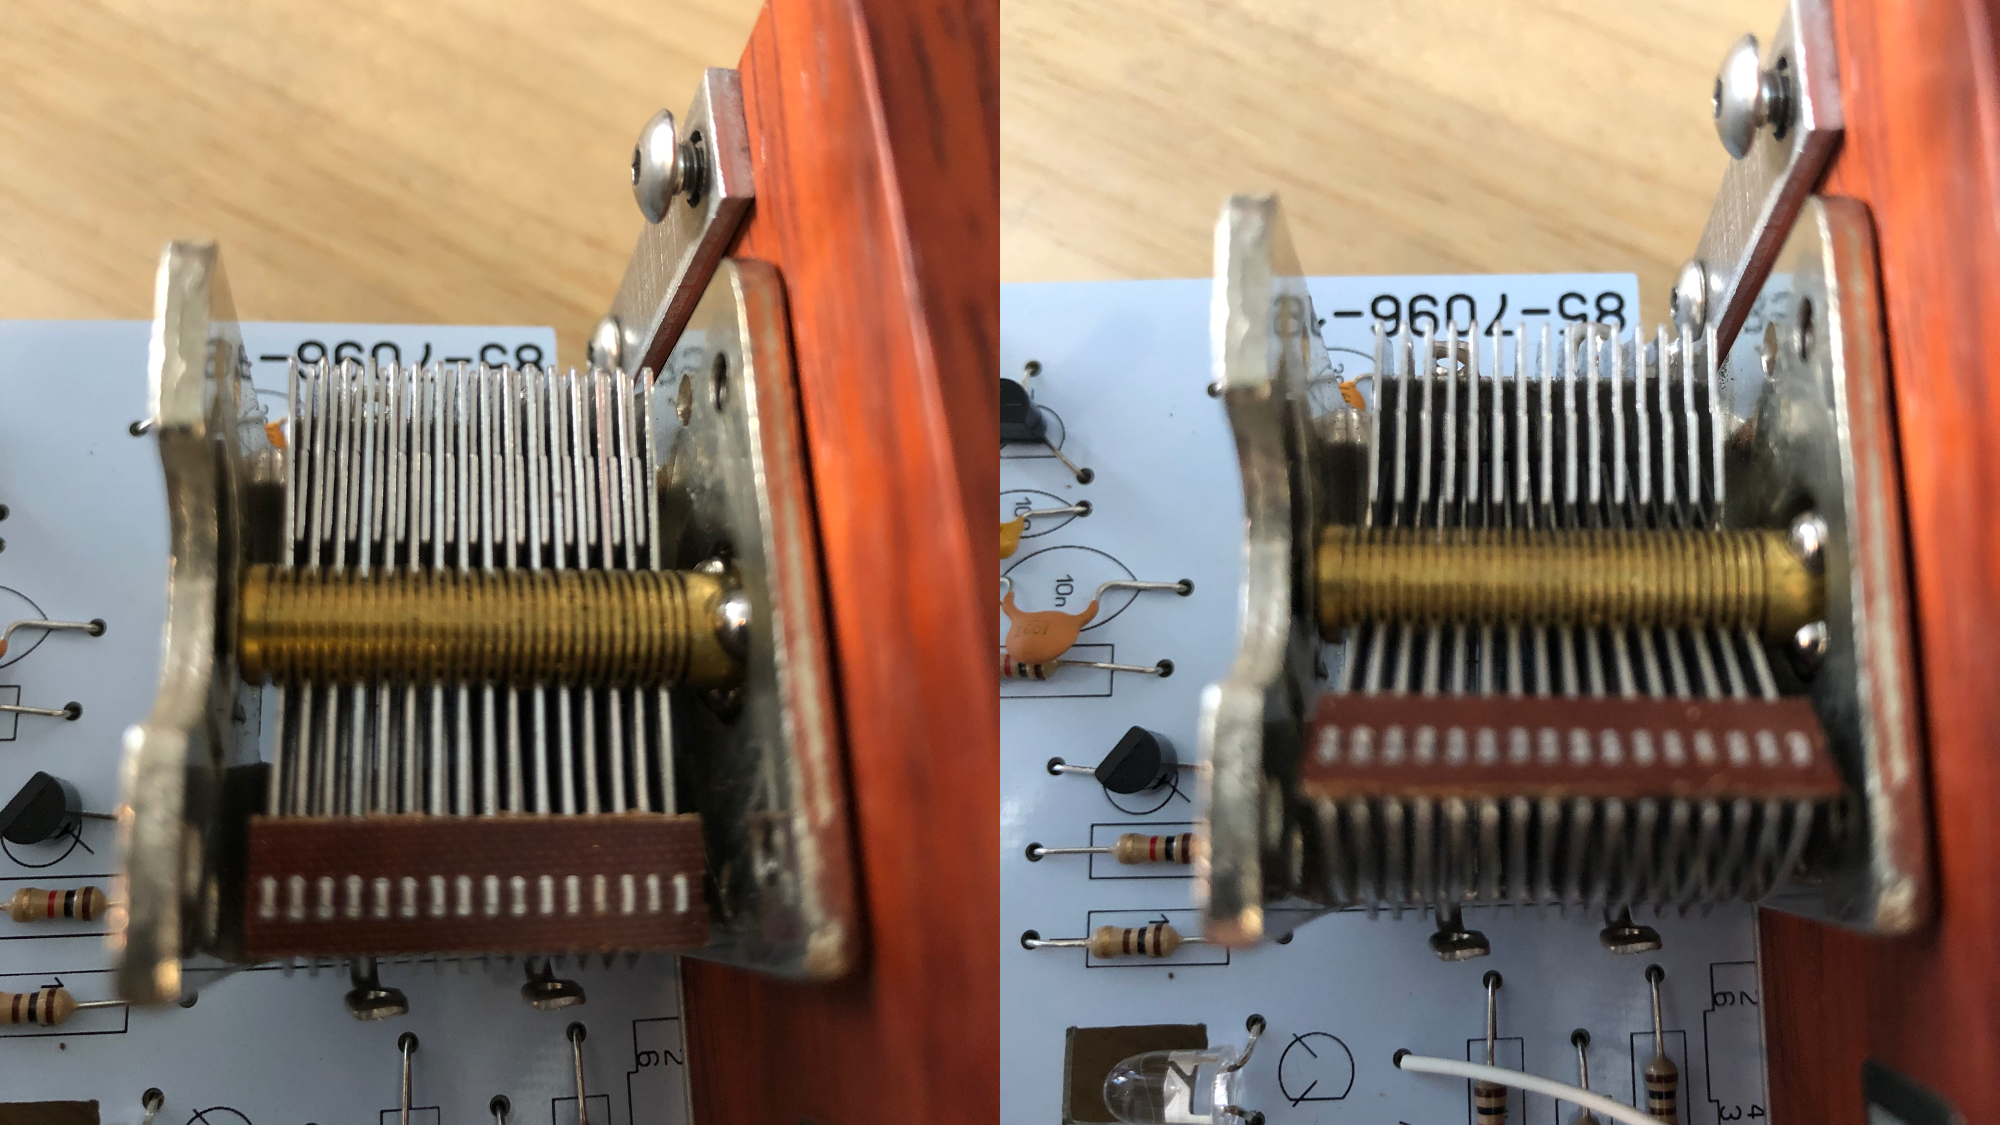
\includegraphics[width=\linewidth]{external/rotary-cap.png}
\end{image}%
\tcblower
\end{figureptx}%
The circuit symbol for a variable capacitor is shown in \hyperref[variablecapsymbol]{Figure~{\xreffont\ref{variablecapsymbol}}}.%
\begin{figureptx}{Figure}{The circuit symbol for a variable capacitor.}{variablecapsymbol}{}%
\begin{image}{0.4}{0.2}{0.4}{}%
\resizebox{\linewidth}{!}{%
\begin{tikzpicture}[font=\sffamily]
	\draw (3,2) to [vC] (0,2);
\end{tikzpicture}%
}%
\end{image}%
\tcblower
\end{figureptx}%
Variable capacitors were used in radio circuits (before they became largely digital) to tune the correct radio frequency to amplify. The dial on the radio literally moved the rotating metal plates to change the capacitance and hence the circuit frequency.%
\end{subsectionptx}
%
%
\typeout{************************************************}
\typeout{Subsection 5.1.3 Polarized Capacitors}
\typeout{************************************************}
%
\begin{subsectionptx}{Subsection}{Polarized Capacitors}{}{Polarized Capacitors}{}{}{ch5-polarcaps}
\ptxterminology{Polarized capacitors} are capacitors where one of the leads must be connected to high potential and the other to low potential. In other words: the capacitor cannot be connected in the circuit any which way. The circuit symbol for a polarized capacitor is shown in \hyperref[polarizedcapsymbol]{Figure~{\xreffont\ref{polarizedcapsymbol}}}. The round end corresponds to the cathode (low potential lead) of the capacitor.%
\begin{figureptx}{Figure}{The circuit symbol for a polarized capacitor.}{polarizedcapsymbol}{}%
\begin{image}{0.4}{0.2}{0.4}{}%
\resizebox{\linewidth}{!}{%
\begin{tikzpicture}[font=\sffamily]
	\draw (3,2) to [cC] (0,2);
\end{tikzpicture}%
}%
\end{image}%
\tcblower
\end{figureptx}%
Polarized capacitors fall into two categories: \ptxterminology{electrolytic capacitors} and \ptxterminology{supercapacitors}. Supercapacitors will not be discussed in this book except to note that they act as a hybrid between a capacitor and a rechargeable battery. Electrolytic capacitors are named after the type of metal used in the anode: aluminum, niobium, or tantalum. Each of the anodes is roughened (which acts to increase the surface area of the capacitor) and oxidized (creating a very thin dielectric layer, decreasing the distance between cathode and anode). An electrolyte gel acts as the cathode. Electrolytic capacitors generally have a very large amount of capacitance. However, because they are polarized, they cannot be used in all circuit applications and are mostly used in DC circuits.%
\par
\ptxterminology{Aluminum electrolytic capacitors} have an aluminum anode. They tend to be inexpensive and easy to obtain. Aluminum electrolytic capacitors are packaged in a cylinder. In a radial configuration, one of the leads is shorter than the other and is situated near a stripe on the cylindrical package. The short lead \slash{} stripe indicates the low potential end of the capacitor. This is depicted in \hyperref[aluminumelectrolyticdiagram]{Figure~{\xreffont\ref{aluminumelectrolyticdiagram}}}.%
\begin{figureptx}{Figure}{Diagram of an aluminum electrolytic capacitor. The short lead (also has a stripe on the casing) corresponds to the low potential connection.}{aluminumelectrolyticdiagram}{}%
\begin{image}{0.45}{0.1}{0.45}{}%
\resizebox{\linewidth}{!}{%
\begin{tikzpicture}[font=\sffamily]
	\tikzset{partial ellipse/.style args={#1:#2:#3}{insert path={+ (#1:#3) arc (#1:#2:#3)}}}
	\draw (-0.25,-1.7) --++ (-0.2,-1.25);
	\draw (0.25,-1.7) --++ (0.2,-1);
	\fill[black] (0.1,-0.2) rectangle (0.3,-1.69);
	\draw[fill=gray!20] (0,0) ellipse (0.5 and 0.25);
	\draw (-0.5,0) --++ (0,-1.5);
	\draw (0.5,0) --++ (0,-1.5);
	\draw[] (0,-1.5) [partial ellipse=0:-180:0.5 and 0.25];
\end{tikzpicture}%
}%
\end{image}%
\tcblower
\end{figureptx}%
The top of the cylindrical packaging is typically scored to allow breakage in case the capacitor is reverse-biased (plugged in backwards) or over-volted. On top of the hazard of over-volting the capacitor, reverse biasing the capacitor is also problematic. Aluminum electrolytic capacitors can and will explode under the right circumstances, and will release anisotropically via the scored top of the cylinder. (Therefore, it is not a good idea to point the top of an aluminum electrolytic capacitor at anything important, especially your face, if it is uncertain if it's connected properly or with the correct amount of voltage). Thankfully, as with ceramic capacitors, an aluminum electrolytic capacitor will fail open (removing itself from the circuit after exploding). The amount of capacitance of an aluminum electrolytic capacitor, as well as the voltage rating, is printed on the packaging.%
\par
\ptxterminology{Tantalum electrolytic capacitors} are made of a tantalum anode. They have a very large capacitance per unit of volume, making them good to use in applications where a small footprint is required. Physically, tantalum electrolytic capacitors resemble the pancake look of a ceramic capacitor. However, tantalum electrolytic capacitors are polarized and must be treated accordingly. Usually, the high potential end (anode) is indicated on the packaging with a plus sign, as shown in \hyperref[tantalumcapdiagram]{Figure~{\xreffont\ref{tantalumcapdiagram}}}.%
\begin{figureptx}{Figure}{A diagram of a tantalum electrolytic capacitor. The plus sign corresponds to the high potential lead.}{tantalumcapdiagram}{}%
\begin{image}{0.45}{0.1}{0.45}{}%
\resizebox{\linewidth}{!}{%
\begin{tikzpicture}[font=\sffamily]
	\draw[fill=gray!20] (0,0)-- (0:0.5) arc (0:180:0.5 and 0.8) -- cycle ;
	\draw (-0.3,0) node[above] {~+} --++ (-0.25,-1.25);
	\draw (0.3,0) --++ (0.25,-1.25);
\end{tikzpicture}%
}%
\end{image}%
\tcblower
\end{figureptx}%
Tantalum capacitors have the property of failing short when over-volted. This can be very dangerous, as a short exacerbates the problem and can lead to a fire. Therefore it is very important to respect the polarity and voltage rating of a tantalum electrolytic capacitor.%
\end{subsectionptx}
\end{sectionptx}
%
%
\typeout{************************************************}
\typeout{Section 5.2 Measuring Capacitance}
\typeout{************************************************}
%
\begin{sectionptx}{Section}{Measuring Capacitance}{}{Measuring Capacitance}{}{}{ch5-measuringcap}
Capacitors can be measured with a digital multimeter or with an LRC meter. A digital multimeter will charge a capacitor with a known current and measure the voltage to calculate the capacitance. An LRC meter applies an AC voltage, measures the AC current, and uses the phase and amplitude differences to calculate the capacitance.%
\par
Capacitance must be measured from one end of the capacitor (or equivalent capacitance) to the other, in parallel, as shown in \hyperref[measuringcapacitance]{Figure~{\xreffont\ref{measuringcapacitance}}}. When measuring the capacitance of a polarized capacitor, it is important to verify that the positive lead of the LRC meter connects to the anode of the capacitor and the negative lead of the LRC meter connects to the cathode of the capacitor.%
\begin{figureptx}{Figure}{A diagram of how capacitance is measured in parallel (across a component or components).}{measuringcapacitance}{}%
\begin{image}{0.35}{0.3}{0.35}{}%
\resizebox{\linewidth}{!}{%
\begin{tikzpicture}[font=\sffamily]
	\draw (0.5,1.5) to [qvprobe] (3.5,1.5);
	\draw[-Stealth] (0.5,1.5) -- (0.5,0);
	\draw[-Stealth] (3.5,1.5) -- (3.5,0);
	\draw (0,0) to [C] (4,0);
\end{tikzpicture}%
}%
\end{image}%
\tcblower
\end{figureptx}%
It is important to ensure that the capacitor(s) are completely discharged before making a measurement. Capacitors can be discharged by shorting the leads with a high value, high-wattage resistor for several seconds.%
\end{sectionptx}
%
%
\typeout{************************************************}
\typeout{Section 5.3 Voltage-Current Relationship in a Capacitor}
\typeout{************************************************}
%
\begin{sectionptx}{Section}{Voltage-Current Relationship in a Capacitor}{}{Voltage-Current Relationship in a Capacitor}{}{}{ch5-vicap}
The relationship between voltage and current in a capacitor can be quantified using the relationship between capacitance and charge (\hyperref[ch5-eqcapqvc]{({\xreffont\ref{ch5-eqcapqvc}})}) as well as the relationship between current and charge (\hyperref[ch1-currentequation]{({\xreffont\ref{ch1-currentequation}})}). This relationship is shown in terms of current in \hyperref[ch5-ivcapequation]{({\xreffont\ref{ch5-ivcapequation}})} and derived in \hyperlink{ch5-cdvdtderivation}{Derivation~{\xreffont 5.3.1}}.%
\par
%
\begin{equation}
i(t) = C\frac{dv(t)}{dt}\label{ch5-ivcapequation}
\end{equation}
%
\begin{proof}{Derivation}{}{ch5-cdvdtderivation}
%
\begin{align*}
i(t) \amp= \frac{dq(t)}{dt}\\
\amp= \frac{d(v(t)C)}{dt}\\
\amp= C\frac{dv(t)}{dt}
\end{align*}
%
\end{proof}
Based on \hyperref[ch5-ivcapequation]{({\xreffont\ref{ch5-ivcapequation}})}, if the voltage remains unchanging through time, there will be no current flowing through the branch that contains a capacitor. Therefore, in DC conditions, a capacitor can be replaced by an open circuit.%
\par
\hyperref[ch5-ivcapequation]{({\xreffont\ref{ch5-ivcapequation}})} can be refigured to solve for the voltage drop over a capacitor, shown in \hyperref[ch5-voltcapequation]{({\xreffont\ref{ch5-voltcapequation}})}.%
\par
%
\begin{equation}
v(t) = \frac{1}{C}\int_{-\infty}^{t} i(\tau)\,d\tau\label{ch5-voltcapequation}
\end{equation}
%
\par
Although calculus is required to fully analyze the relationship between voltage and current in a capacitor, the relationship between the two variables is linear. This means that capacitors are linear circuit elements, and all of the techniques discussed in this book (superposition and Thévenin equivalence, for example) are still applicable with capacitive circuits.%
\end{sectionptx}
%
%
\typeout{************************************************}
\typeout{Section 5.4 Equivalent Capacitance}
\typeout{************************************************}
%
\begin{sectionptx}{Section}{Equivalent Capacitance}{}{Equivalent Capacitance}{}{}{ch5-equivalentcap}
\begin{introduction}{}%
Just as it was possible to combine resistors together to find an equivalent resistance, it is possible to combine capacitors together to find an equivalent capacitance. The rules (and mathematical relationships) for calculating series and parallel combinations of capacitors are explained below.%
\end{introduction}%
%
%
\typeout{************************************************}
\typeout{Subsection 5.4.1 Series Combinations of Capacitors}
\typeout{************************************************}
%
\begin{subsectionptx}{Subsection}{Series Combinations of Capacitors}{}{Series Combinations of Capacitors}{}{}{ch5-seriescaps}
Capacitors in series all share a common branch, as shown in \hyperref[seriescapsfig]{Figure~{\xreffont\ref{seriescapsfig}}}. Each individual voltage drop is shown (numbered with subscripts), as well as the total voltage drop over the combination of capacitors (\(v(t)\)). The current through all of the capacitors is the same and is labeled \(i(t)\).%
\begin{figureptx}{Figure}{Five capacitors in series in a circuit.}{seriescapsfig}{}%
\begin{image}{0.05}{0.9}{0.05}{}%
\resizebox{\linewidth}{!}{%
\begin{tikzpicture}[font=\sffamily]
	\draw (0,0) to [C, v^=$v_1(t)$] (2,0);
	\draw (2,0) to [C, v^=$v_2(t)$] (4,0);
	\draw (4,0) to [C, v^=$v_3(t)$] (6,0);
	\draw (6,0) to [C, v^=$v_4(t)$] (8,0);
	\draw (8,0) to [C, v^=$v_5(t)$, i_>=$i(t)$] (10,0);
	\draw (0,1.5) to [open, v^=$v(t)$] (10,1.5);
\end{tikzpicture}%
}%
\end{image}%
\tcblower
\end{figureptx}%
As \(v(t)\) is equal to the sum of each individual voltage drop, the current-voltage relationship in capacitors (\hyperref[ch5-voltcapequation]{({\xreffont\ref{ch5-voltcapequation}})}) can be used to determine the equivalent capacitance of series combinations of capacitors. This is given in \hyperref[ch5-seriescapequation]{({\xreffont\ref{ch5-seriescapequation}})} and derived in \hyperlink{ch5-seriescapderivation}{Derivation~{\xreffont 5.4.1.1}}.%
\par
%
\begin{equation}
\frac{1}{C_{EQ}} = \frac{1}{C_1} + \frac{1}{C_2} + \frac{1}{C_3} + ... + \frac{1}{C_n}\label{ch5-seriescapequation}
\end{equation}
%
\begin{proof}{Derivation}{}{ch5-seriescapderivation}
%
\begin{align*}
v(t) \amp= v_1(t) + v_2(t) + v_3(t) + ... + v_n(t)\\
\int_{-\infty}^{t} \frac{1}{C_{EQ}} i(\tau)\,d\tau \amp= \int_{-\infty}^{t} \frac{1}{C_1} i(\tau)\,d\tau + \int_{-\infty}^{t} \frac{1}{C_2} i(\tau)\,d\tau + \int_{-\infty}^{t} \frac{1}{C_3} i(\tau)\,d\tau + ... + \int_{-\infty}^{t} \frac{1}{C_n} i(\tau)\,d\tau\\
\frac{1}{C_{EQ}} \int_{-\infty}^{t} i(\tau)\,d\tau \amp= \frac{1}{C_1} \int_{-\infty}^{t} i(\tau)\,d\tau + \frac{1}{C_2} \int_{-\infty}^{t} i(\tau)\,d\tau + \frac{1}{C_3} \int_{-\infty}^{t} i(\tau)\,d\tau + ... + \frac{1}{C_n} \int_{-\infty}^{t} i(\tau)\,d\tau\\
\frac{1}{C_{EQ}} \amp= \frac{1}{C_1} + \frac{1}{C_2} + \frac{1}{C_3} + ... + \frac{1}{C_n}
\end{align*}
%
\end{proof}
Capacitors in series therefore combine similarly to resistors in parallel. The equivalent capacitance cannot be larger than the smallest capacitor in the series combination.%
\end{subsectionptx}
%
%
\typeout{************************************************}
\typeout{Subsection 5.4.2 Parallel Combinations of Capacitors}
\typeout{************************************************}
%
\begin{subsectionptx}{Subsection}{Parallel Combinations of Capacitors}{}{Parallel Combinations of Capacitors}{}{}{ch5-parallelcaps}
Capacitors in parallel all share two nodes, as shown in \hyperref[parallelcapdiagram]{Figure~{\xreffont\ref{parallelcapdiagram}}}. Each individual current is shown (numbered with subscripts), as well as the total current through the combination of capacitors (\(i(t)\)). The voltage drop over all of the capacitors is the same and is labeled \(v(t)\).%
\begin{figureptx}{Figure}{Five capacitors in parallel in a circuit.}{parallelcapdiagram}{}%
\begin{image}{0.15}{0.7}{0.15}{}%
\resizebox{\linewidth}{!}{%
\begin{tikzpicture}[font=\sffamily]
	\def\spacing{1.75}
	\foreach \x in {1, 2, 3, 4, 5} {
		\draw[]	(\x*\spacing,0) to [C, i_=$i_\x(t)$] ++(down:2.5);
	}
	\draw[]	(5.5*\spacing,0) to [open, v^=$v(t)$]	++(down:2.5);
	\draw[]	(3*\spacing,1) to [short, i_=$i(t)$, -*] ++(down:1);
	\draw[]	(3*\spacing,-2.5) to [short, *-] ++(down:1);
	\draw[]	(\spacing,0) to [short, -*] ++(right:\spacing) to [short, -*] ++(right:2*\spacing) --++ (right:\spacing);
	\draw[]	(\spacing,-2.5) to [short, -*] ++(right:\spacing) to [short, -*] ++(right:2*\spacing) --++ (right:\spacing);
\end{tikzpicture}%
}%
\end{image}%
\tcblower
\end{figureptx}%
As \(i(t)\) is equal to the sum of each individual current, the current-voltage relationship in capacitors (\hyperref[ch5-ivcapequation]{({\xreffont\ref{ch5-ivcapequation}})}) can be used to determine the equivalent capacitance of parallel combinations of capacitors. This is shown in \hyperref[parallelcapequation]{({\xreffont\ref{parallelcapequation}})} and derived in \hyperlink{parallelcapderivation}{Derivation~{\xreffont 5.4.2.1}}.%
\par
%
\begin{equation}
C_{EQ} = C_1 + C_2 + C_3 + ... + C_n\label{parallelcapequation}
\end{equation}
%
\begin{proof}{Derivation}{}{parallelcapderivation}
%
\begin{align*}
i(t) \amp= i_1(t) + i_2(t) + i_3(t) + ... + i_n(t)\\
C_{EQ}\frac{dv(t)}{dt} \amp= C_1\frac{dv(t)}{dt} + C_2\frac{dv(t)}{dt} + C_3\frac{dv(t)}{dt} + ... + C_4\frac{dv(t)}{dt}\\
C_{EQ} \amp= C_1 + C_2 + C_3 + ... + C_n
\end{align*}
%
\end{proof}
Capacitors in parallel therefore combine similarly to resistors in series. The equivalent capacitance cannot be smaller than the largest capacitor in the parallel combination.%
\begin{example}{Example}{Calculating equivalent capacitance.}{ch5-parallelcaps-8}%
Calculate the equivalent capacitance between nodes a and b in the circuit shown in \hyperref[equivalentcapacitanceex1]{Figure~{\xreffont\ref{equivalentcapacitanceex1}}}.%
\begin{figureptx}{Figure}{}{equivalentcapacitanceex1}{}%
\begin{image}{0.15}{0.7}{0.15}{}%
\resizebox{\linewidth}{!}{%
\begin{tikzpicture}[font=\sffamily]
	\foreach \x/\y/\c/\dir/\o in {0/0/3/down/4, 2/0/6/left/2, 4/0/5/left/2, 4/0/3/down/2, 4/-2/8/down/2, 6/0/2/left/2, 6/0/6/down/4} {
		\draw[]	(\x,\y) to [C, l_=\c~$\mu$F]	++(\dir:\o);
	}
	\draw[]	(-1,0) node[left] {a} to [short, o-*] ++(right:1);
	\draw[]	(-1,-4) node[left] {b} to [short, o-*] ++(right:1) to [short, -*] ++(right:4) --++ (right:2);
	\node[circ]	at (4,0) {};
\end{tikzpicture}%
}%
\end{image}%
\tcblower
\end{figureptx}%
The 2~µF and 6~µF are in series and can be combined together. This combination is 1.5~µF. Similarly, the 3~µF is in series with the 8~µF with an equivalent capacitance of of 2.18~µF. Last, the 6~µF and 5~µF capacitors are in series with an equivalent capacitance of 2.73~µF. The circuit can now be re-drawn.%
\begin{figureptx}{Figure}{}{ch5-parallelcaps-8-2-4}{}%
\begin{image}{0.2}{0.6}{0.2}{}%
\resizebox{\linewidth}{!}{%
\begin{tikzpicture}[font=\sffamily]
	\foreach \x/\y/\c/\dir/\o in {0/0/3/down/2.5, 2.5/0/2.73/left/2.5, 2.5/0/2.18/down/2.5, 5/0/1.5/down/2.5} {
		\draw[]	(\x,\y) to [C, l_=\c~$\mu$F]	++(\dir:\o);
	}
	\draw[]	(-1,0) node[left] {a} to [short, o-*] ++(right:1);
	\draw[]	(-1,-2.5) node[left] {b} to [short, o-*] ++(right:1) to [short, -*] ++(right:2.5) --++ (right:2.5);
	\draw[]	(2.5,0) to [short, *-] ++(right:2.5);
\end{tikzpicture}%
}%
\end{image}%
\tcblower
\end{figureptx}%
At this point the 1.5~µF and 2.18~µF capacitors can be combined in parallel to obtain. 3.68~µF. The circuit can again be re-drawn.%
\begin{figureptx}{Figure}{}{ch5-parallelcaps-8-2-6}{}%
\begin{image}{0.3}{0.4}{0.3}{}%
\resizebox{\linewidth}{!}{%
\begin{tikzpicture}[font=\sffamily]
	\foreach \x/\y/\c/\dir/\o in {0/0/3/down/2.5, 2.5/0/2.73/left/2.5, 2.5/0/3.68/down/2.5} {
		\draw[]	(\x,\y) to [C, l_=\c~$\mu$F]	++(\dir:\o);
	}
	\draw[]	(-1,0) node[left] {a} to [short, o-*] ++(right:1);
	\draw[]	(-1,-2.5) node[left] {b} to [short, o-*] ++(right:1) --++(right:2.5);
\end{tikzpicture}%
}%
\end{image}%
\tcblower
\end{figureptx}%
The 2.73~µF capacitor is in series with the 3.68~µF capacitor. Combined, their equivalent capacitance is 1.57~µF. The circuit can be re-drawn again.%
\begin{figureptx}{Figure}{}{ch5-parallelcaps-8-2-8}{}%
\begin{image}{0.3}{0.4}{0.3}{}%
\resizebox{\linewidth}{!}{%
\begin{tikzpicture}[font=\sffamily]
	\foreach \x/\y/\c/\dir/\o in {0/0/3/down/2.5, 2.5/0/1.57/down/2.5} {
		\draw[]	(\x,\y) to [C, l_=\c~$\mu$F]	++(\dir:\o);
	}
	\draw[]	(-1,0) node[left] {a} to [short, o-*] ++(right:1) --++ (right:2.5);
	\draw[]	(-1,-2.5) node[left] {b} to [short, o-*] ++(right:1) --++(right:2.5);
\end{tikzpicture}%
}%
\end{image}%
\tcblower
\end{figureptx}%
The equivalent capacitance can now be calculated by summing together the two capacitances.%
\par
%
\begin{equation*}
C_{EQ} = 4.57~\mu\textrm{F}
\end{equation*}
%
\end{example}
\end{subsectionptx}
\end{sectionptx}
%
%
\typeout{************************************************}
\typeout{Section 5.5 Differentiator and Integrator Circuits}
\typeout{************************************************}
%
\begin{sectionptx}{Section}{Differentiator and Integrator Circuits}{}{Differentiator and Integrator Circuits}{}{}{ch5-differentiatorintegrator}
The current-voltage relationship in a capacitor can be used to create circuits capable of calculating the derivative or integral of a signal.%
\par
First, consider the circuit shown in \hyperref[opampdifffigure]{Figure~{\xreffont\ref{opampdifffigure}}}. This is a differentiator circuit. The output voltage is directly proportional to the derivative of the input voltage.%
\begin{figureptx}{Figure}{Op-amp differentiator circuit.}{opampdifffigure}{}%
\begin{image}{0.2}{0.6}{0.2}{}%
\resizebox{\linewidth}{!}{%
\begin{tikzpicture}[font=\sffamily]
	\draw[]	(3.5,1) node[op amp] (opamp) {};
	\draw[]	(opamp.out) to [short, *-] ++ (right:0.5) node[right] {$v_{out}(t)$};
	\draw[]	(opamp.+) node[ground] {};
	\draw[]	(opamp.-) to [short, *-] ++(up:1.25) to [R, l^=$R$] ++ (right:2.25) -| (opamp.out);
	\draw[]	($(opamp.-)-(2,0)$) to [sV, l_=$v_{in}(t)$] ($(opamp.-)-(2,1.5)$) node[ground] {};
	\draw[]	($(opamp.-)-(2,0)$) node[below left] {+} to [C, l^=$C$] (opamp.-);
\end{tikzpicture}%
}%
\end{image}%
\tcblower
\end{figureptx}%
The current through the capacitor can be described by \hyperref[ch5-ivcapequation]{({\xreffont\ref{ch5-ivcapequation}})}. Assume the direction of current is from left to right in both the resistor and the capacitor in \hyperref[opampdifffigure]{Figure~{\xreffont\ref{opampdifffigure}}}. The voltage drop over the capacitor is therefore \(v_{in}(t)\). The output voltage of the circuit can then be described in \hyperref[ch5-equationdiffoutput]{({\xreffont\ref{ch5-equationdiffoutput}})}, which is derived in \hyperlink{ch5-differentiatorcircuitderivation}{Derivation~{\xreffont 5.5.1}}.%
\par
%
\begin{equation}
v_{out}(t) = -RC \frac{d}{dt}v_{in}(t)\label{ch5-equationdiffoutput}
\end{equation}
%
\begin{proof}{Derivation}{}{ch5-differentiatorcircuitderivation}
%
\begin{align*}
C\frac{d}{dt} v_{in}(t) \amp= -\frac{v_{out}(t)}{R}\\
-RC \frac{d}{dt} v_{in}(t) \amp= v_{out}(t)
\end{align*}
%
\end{proof}
Next, consider the circuit shown in \hyperref[opampintegratorfigure]{Figure~{\xreffont\ref{opampintegratorfigure}}}. This is an integrator circuit. The output voltage is directly proportional to the integral of the input voltage.%
\begin{figureptx}{Figure}{Op-amp integrator circuit.}{opampintegratorfigure}{}%
\begin{image}{0.2}{0.6}{0.2}{}%
\resizebox{\linewidth}{!}{%
\begin{tikzpicture}[font=\sffamily]
	\draw[]	(3.5,1) node[op amp] (opamp) {};
	\draw[]	(opamp.out) to [short, *-] ++ (right:0.5) node[right] {$v_{out}(t)$};
	\draw[]	(opamp.+) node[ground] {};
	\draw[]	(opamp.-) to [short, *-] ++(up:1.25) to [C, l^=$C$] ++(right:2.25) -| (opamp.out);
	\draw[]	($(opamp.-)-(2,0)$) to [sV, l_=$v_{in}(t)$] ($(opamp.-)-(2,1.5)$) node[ground] {};
	\draw[]	($(opamp.-)-(2,0)$) node[below left] {+} to [R, l^=$R$] (opamp.-);
\end{tikzpicture}%
}%
\end{image}%
\tcblower
\end{figureptx}%
The current through the capacitor can be described by \hyperref[ch5-ivcapequation]{({\xreffont\ref{ch5-ivcapequation}})}. Assume the direction of current is from left to right in both the resistor and the capacitor in \hyperref[opampintegratorfigure]{Figure~{\xreffont\ref{opampintegratorfigure}}}. The voltage drop over the capacitor is therefore \(-v_{out}(t)\). The output voltage of the circuit can then be described in \hyperref[ch5-integratoroutputequation]{({\xreffont\ref{ch5-integratoroutputequation}})}, which is derived in \hyperlink{ch5-integratorequationderivation}{Derivation~{\xreffont 5.5.2}}.%
\par
%
\begin{equation}
v_{out}(t) = -\frac{1}{RC}\int v_{in}(t) \,dt\label{ch5-integratoroutputequation}
\end{equation}
%
\begin{proof}{Derivation}{}{ch5-integratorequationderivation}
%
\begin{align*}
\frac{v_{in}(t)}{R} \amp= C\frac{d}{dt}\left[-v_{out}(t)\right]\\
\int \frac{v_{in}(t)}{R}\, dt \amp= \int C\frac{d}{dt}\left[-v_{out}(t)\right]\, dt\\
\frac{1}{R} \int v_{in}(t) \, dt \amp= -C v_{out}(t)\\
-\frac{1}{CR} \int v_{in}(t) \, dt \amp= v_{out}(t)
\end{align*}
%
\end{proof}
\end{sectionptx}
%
%
\typeout{************************************************}
\typeout{Section 5.6 Review of Important Mathematical Concepts for First-Order Circuits}
\typeout{************************************************}
%
\begin{sectionptx}{Section}{Review of Important Mathematical Concepts for First-Order Circuits}{}{Review of Important Mathematical Concepts for First-Order Circuits}{}{}{ch5-review}
\begin{introduction}{}%
The resistor-capacitor circuits that will be introduced in \hyperref[ch5-rccircuits]{Section~{\xreffont\ref{ch5-rccircuits}}} (and the resistor-inductor circuits that will be introduced in \hyperref[ch6-resistor-inductor-circuits]{Section~{\xreffont\ref{ch6-resistor-inductor-circuits}}}) represent linear, first-order circuits. Their voltage and current measurements will represent functions that are the solution to a linear, first-order, ordinary differential equation. The important concepts from these two topics will be reintroduced here to reinforce the concepts that are most important to analyzing circuits.%
\end{introduction}%
%
%
\typeout{************************************************}
\typeout{Subsection 5.6.1 Discontinuous Functions}
\typeout{************************************************}
%
\begin{subsectionptx}{Subsection}{Discontinuous Functions}{}{Discontinuous Functions}{}{}{ch5-discontinuous}
The discontinuous functions that will occur in this textbook will contain an abrupt change in function values at a single point. For example, \hyperref[ch5-discontinuouscurrent]{Figure~{\xreffont\ref{ch5-discontinuouscurrent}}} is a representative example of the current through a capacitor when it is abruptly disconnected from power at \(t = 0\). The function is discontinuous at \(t = 0\).%
\begin{figureptx}{Figure}{An example graph of current through a capacitor after being removed from a source at \(t = 0\).}{ch5-discontinuouscurrent}{}%
\begin{image}{0}{1}{0}{}%
\resizebox{\linewidth}{!}{%
\begin{tikzpicture}[font=\sffamily]
	\begin{axis}[xlabel=$t$~(ms), ylabel=$i(t)$~(mA), xmin=-3, xmax=12, width=\linewidth, height=5cm]
		\addplot[thick] coordinates {(-3,0) (0,0)};
		\addplot[only marks,fill=white,mark=*]coordinates{(0,0)};
		\addplot[only marks,mark=*]coordinates{(0,-1)};
		\addplot[thick, domain=0:20, samples=50] {-1*exp(-0.3*x)};
				\end{axis}
\end{tikzpicture}%
}%
\end{image}%
\tcblower
\end{figureptx}%
The value of the function at \(t = 0\) is represented by the filled black dot. In \hyperref[ch5-discontinuouscurrent]{Figure~{\xreffont\ref{ch5-discontinuouscurrent}}}, the value of the current at \(t = 0\) is -1~mA.%
\par
Three values can be used to describe the value of a function at a discontinuity located at \(t = t_0\):%
\par
%
\begin{itemize}[label=\ptxlistdisc]
\item{}\(f(t_0)\): this is equal to the defined value of the function at \(t_0\). (In the example shown in \hyperref[ch5-discontinuouscurrent]{Figure~{\xreffont\ref{ch5-discontinuouscurrent}}}, \(i(0) = -1~\textrm{mA}\).)%
\item{}\(f(t_0^+)\): this is equal to the value of the function at \(t_0\) when approaching \(\tau\) from the right. (In the example shown in \hyperref[ch5-discontinuouscurrent]{Figure~{\xreffont\ref{ch5-discontinuouscurrent}}}, \(i(0^+) = -1~\textrm{mA}\).)%
\item{}\(f(t_0^-)\): this is equal to the value of the function at \(t_0\) when approaching \(\tau\) from the left. (In the example shown in \hyperref[ch5-discontinuouscurrent]{Figure~{\xreffont\ref{ch5-discontinuouscurrent}}}, \(i(0^-) = 0~\textrm{mA}\).)%
\end{itemize}
%
\par
Another example of a discontinuous function is the step function, introduced in \hyperref[ch1-stepfunction]{Subsection~{\xreffont\ref{ch1-stepfunction}}}.%
\end{subsectionptx}
%
%
\typeout{************************************************}
\typeout{Subsection 5.6.2 First-Order, Linear, Ordinary Differential Equations}
\typeout{************************************************}
%
\begin{subsectionptx}{Subsection}{First-Order, Linear, Ordinary Differential Equations}{}{First-Order, Linear, Ordinary Differential Equations}{}{}{ch5-first-order-linear-ODEs}
The circuits described in this chapter and in \hyperref[ch6-inductors]{Chapter~{\xreffont\ref{ch6-inductors}}} represent first-order, linear circuits. Analysis of the circuits will yield a first-order, linear, ordinary differential equation with constant coefficients.%
\par
%
\begin{itemize}[label=\ptxlistdisc]
\item{}First-order describes the highest-order derivative in the equation. A first-order equation has a first-derivative term and no higher-order derivatives.%
\item{}Linear describes the operations that occur on the function. If the operations are linear, then the equation is linear.%
\item{}Ordinary describes the types of derivatives in the equation. If there are no partial derivatives, then the equation is ordinary.%
\end{itemize}
%
\par
An example of a first-order, linear, ordinary differential equation with constant coefficients is shown in \hyperref[ch5-firstorderlinearode]{({\xreffont\ref{ch5-firstorderlinearode}})}.%
\par
%
\begin{equation}
a_1 \frac{df(t)}{dt} + a_0 f(t) = y(t)\label{ch5-firstorderlinearode}
\end{equation}
%
\par
In this textbook, we will derive equations in \ptxterminology{standard form}, which means that the coefficient of the highest-order derivative term (\(a_1\) in \hyperref[ch5-firstorderlinearode]{({\xreffont\ref{ch5-firstorderlinearode}})}) will be equal to one. When in standard form, first-order equations can be described as shown in \hyperref[ch5-firstorderlinearode-standard]{({\xreffont\ref{ch5-firstorderlinearode-standard}})}, where \(\tau\) is known as the \ptxterminology{time constant} of the circuit.%
\par
%
\begin{equation}
\frac{df(t)}{dt} + \frac{1}{\tau} f(t) = y(t)\label{ch5-firstorderlinearode-standard}
\end{equation}
%
\par
When the function \(y(t)\) as defined in \hyperref[ch5-firstorderlinearode-standard]{({\xreffont\ref{ch5-firstorderlinearode-standard}})} is equal to zero, the equation is said to be \ptxterminology{homogeneous}, otherwise the equation is non-homogeneous. In this chapter and in \hyperref[ch6-inductors]{Chapter~{\xreffont\ref{ch6-inductors}}}, \(y(t)\) will either be zero (homogeneous) or equal to a constant (non-homogeneous). This textbook will introduce non-constant non-homogeneous solutions in \hyperref[ch7-secondorder]{Chapter~{\xreffont\ref{ch7-secondorder}}} and cover them in detail in \hyperref[ch11-laplace]{Chapter~{\xreffont\ref{ch11-laplace}}}, which will provide a much simpler method for solving this type of circuit.%
\par
In order to obtain the exact solution of a first-order, linear, ordinary differential equation, we will need to know the initial value of the function being described by the equation. If the equation is non-homogeneous, we will also need to know the value of the particular solution. In the non-homogeneous circuits introduced in this chapter and in \hyperref[ch6-inductors]{Chapter~{\xreffont\ref{ch6-inductors}}}, the particular solution will be equal to the final steady-state value of the function being described by the equation.%
\par
The solution to these types of differential equations will be provided in subsequent sections of this textbook after describing how to derive the differential equations.%
\end{subsectionptx}
\end{sectionptx}
%
%
\typeout{************************************************}
\typeout{Section 5.7 Resistor-Capacitor (RC) Circuits}
\typeout{************************************************}
%
\begin{sectionptx}{Section}{Resistor-Capacitor (RC) Circuits}{}{Resistor-Capacitor (RC) Circuits}{}{}{ch5-rccircuits}
\begin{introduction}{}%
Resistor-capacitor (RC) circuits are circuits that contain one capacitor (or combinations of capacitors that can be reduced down to one equivalent capacitance) as well as at least one resistive element. In this chapter, the analysis of these circuits will be performed when DC conditions are changed suddenly to another set of DC conditions. For example: a capacitor will have been subjected to a constant initial voltage for a long period of time, and then suddenly disconnected from a circuit. Or: a capacitor will have been discharged for a long period of time before suddenly being connected to a circuit with a DC voltage. This short-term change in voltage and current is known as a \ptxterminology{transient analysis}.%
\par
Resistors by themselves are incapable of having a transient change. This is because they do not store energy. Because a capacitor stores energy, it is able to experience a transient change in response to changing voltage or current conditions of the circuit.%
\par
On the other hand, a \ptxterminology{steady-state analysis} considers the operation of a circuit when conditions remain steady for a long period of time. In this chapter, the steady-state analysis will only include DC sources. To analyze the behavior of a capacitor in a DC steady-state condition, recall from \hyperref[ch5-vicap]{Section~{\xreffont\ref{ch5-vicap}}}:%
\begin{quote}%
Based on \hyperref[ch5-ivcapequation]{({\xreffont\ref{ch5-ivcapequation}})}, if the voltage remains unchanging through time, there will be no current flowing through the branch that contains a capacitor. Therefore, in DC conditions, a capacitor can be replaced by an open circuit.%
\end{quote}
An important property of capacitors that will aid in the analysis of the transient response is that \ptxalert{the voltage over a capacitor cannot change instantaneously}. That is: \(v_C(0^-)=v_C(0^+)\). In an ideal analysis (which is what this book will use) where capacitors have no parasitic effects (stray inductance, for example), the current through a capacitor can change instantaneously and therefore be discontinuous in time.%
\par
The procedure for analyzing the transient response of an RC circuit includes the following steps.%
\par
%
\begin{enumerate}
\item{}Calculate the initial voltage drop (\(v(0)\)) over the circuit element by analyzing the circuit in its initial steady-state condition. (If necessary, calculate at time \(t=0^-\) and at time \(t=0^+\).)%
\item{}Calculate the final voltage drop (\(v(\infty)\)) over the circuit element by analyzing the circuit in its final steady-state condition.%
\item{}If there are no dependent sources: At time \(t=0^+\), disconnect all independent sources and calculate the equivalent resistance seen by the capacitor. Use this value to calculate the time constant of the circuit.%
\item{}If there are dependent sources or op-amps in the circuit: Either calculate the Thévenin equivalent circuit and use the Thévenin equivalent resistance as the equivalent resistance as seen by the capacitor or derive the differential equation for the circuit and use \hyperref[ch5-firstorderlinearode-standard]{({\xreffont\ref{ch5-firstorderlinearode-standard}})} to calculate the time constant of the circuit.%
\item{}Plug the above values into the equation for \(v(t)\).%
\item{}Use the equation relating voltage and current for the circuit element of interest to derive an equation for \(i(t)\).%
\end{enumerate}
%
\par
All RC circuits can be analyzed in this method to derive a transient response. Before considering circuits of this type in \hyperref[ch5-generaltransient]{Subsection~{\xreffont\ref{ch5-generaltransient}}}, we will first look at two special conditions of the transient response: the homogeneous transient response (i.e. \(v(\infty) = 0\)) and the charging from zero transient response (i.e. \(v(0) = 0\)).%
\end{introduction}%
%
%
\typeout{************************************************}
\typeout{Subsection 5.7.1 Discharging to Zero (Homogeneous) Transient Response}
\typeout{************************************************}
%
\begin{subsectionptx}{Subsection}{Discharging to Zero (Homogeneous) Transient Response}{}{Discharging to Zero (Homogeneous) Transient Response}{}{}{ch5-discharging}
The discharging to zero response is a special case of the transient response that specifically looks at what happens when a capacitor is initially connected to one or more sources that are suddenly removed from a circuit at a particular time. In other words: the capacitor, after being disconnected from the power supply, discharges its stored energy through the resistive element(s) of the circuit. The circuit diagram shown in \hyperref[homogeneousrccircuitfigure]{Figure~{\xreffont\ref{homogeneousrccircuitfigure}}} will be used to analyze this discharging response. The switch is in position a for a long time before suddenly moving to position b at time \(t=0\).%
\begin{figureptx}{Figure}{An RC circuit used to analyze the homogeneous transient response.}{homogeneousrccircuitfigure}{}%
\begin{image}{0.25}{0.5}{0.25}{}%
\resizebox{\linewidth}{!}{%
\begin{tikzpicture}[font=\sffamily]
	\draw[]	(2,1) node[cute spdt up arrow, rotate=90, anchor=in] (switch) {};
	\draw[]	(switch.in) to [C, l_=$C$, v^=$v(t)$, i_=$i(t)$, -*] ++(down:2) node[ground] {};
	\draw[]	(switch.out 1) node[below left] {a} to [short] ++(left:1.75) to [V, l_=$V_{IN}$] ++(down:2.5) |- ($(switch.in)-(0,2)$);
	\draw[]	(switch.out 2) node[below right] {b} to [short] ++(right:1.75) to [R, l_=$R$, i^=$i_R(t)$] ++(down:2.5) |- ($(switch.in)-(0,2)$);
\end{tikzpicture}%
}%
\end{image}%
\tcblower
\end{figureptx}%
The differential equation for the circuit will be derived at the instant the switch changes position at \(t = 0^+\). The circuit diagram in this condition is shown in \hyperref[homogeneousrcatzeroplus]{Figure~{\xreffont\ref{homogeneousrcatzeroplus}}}. (In general, the differential equation does not need to be re-derived for other RC circuits unless the circuit contains one or more dependent sources or op-amps. In those scenarios, the differential equation can be derived to calculate the time constant of the circuit, but it is not explicitly necessary.)%
\begin{figureptx}{Figure}{The RC circuit from \hyperref[homogeneousrccircuitfigure]{Figure~{\xreffont\ref{homogeneousrccircuitfigure}}} drawn at \(t = 0^+\).}{homogeneousrcatzeroplus}{}%
\begin{image}{0.25}{0.5}{0.25}{}%
\resizebox{\linewidth}{!}{%
\begin{tikzpicture}[font=\sffamily]
	\draw[]	(2,1) node[cute spdt down, rotate=90, anchor=in] (switch) {};
	\draw[]	(switch.in) to [C, l_=$C$, v^=$v(t)$, i_=$i(t)$, -*] ++(down:2) node[ground] {};
	\draw[]	(switch.out 1) node[below left] {a} to [short] ++(left:1.75) to [V, l_=$V_{IN}$] ++(down:2.5) |- ($(switch.in)-(0,2)$);
	\draw[]	(switch.out 2) node[below right] {b} to [short] ++(right:1.75) to [R, l_=$R$, i^=$i_R(t)$] ++(down:2.5) |- ($(switch.in)-(0,2)$);
\end{tikzpicture}%
}%
\end{image}%
\tcblower
\end{figureptx}%
Kirchhoff's laws can be used to derive the differential equation describing this circuit. The capacitor and resistor are in series with each other. Therefore, the current through both elements must be equal. Because the direction \(i_R(t)\) opposes the direction of \(i(t)\), a negative sign is used in this relationship, defined in \hyperref[ch5-kclhomogeneousrc]{({\xreffont\ref{ch5-kclhomogeneousrc}})}.%
\par
%
\begin{equation}
i_R(t) = -i(t)\label{ch5-kclhomogeneousrc}
\end{equation}
%
\par
The voltage-current relationship in a capacitor (\hyperref[ch5-ivcapequation]{({\xreffont\ref{ch5-ivcapequation}})}) can be used to define the current through the capacitor, defined in \hyperref[ch5-cdvdthomogeneousrc]{({\xreffont\ref{ch5-cdvdthomogeneousrc}})}.%
\par
%
\begin{equation}
C\frac{dv(t)}{d(t)} = i(t)\label{ch5-cdvdthomogeneousrc}
\end{equation}
%
\par
Ohm's law can be used to relate the current through the resistor and the voltage dropped over the resistor. Because the resistor and capacitor are in parallel, both share an equivalent voltage drop of \(v(t)\). This relationship is defined in \hyperref[ch5-ohmshomogeneousrc]{({\xreffont\ref{ch5-ohmshomogeneousrc}})}.%
\par
%
\begin{equation}
i_R(t) = \frac{v(t)}{R}\label{ch5-ohmshomogeneousrc}
\end{equation}
%
\par
Plug \hyperref[ch5-cdvdthomogeneousrc]{({\xreffont\ref{ch5-cdvdthomogeneousrc}})} and \hyperref[ch5-ohmshomogeneousrc]{({\xreffont\ref{ch5-ohmshomogeneousrc}})} into \hyperref[ch5-kclhomogeneousrc]{({\xreffont\ref{ch5-kclhomogeneousrc}})} and put the equation into standard form as described in \hyperref[ch5-first-order-linear-ODEs]{Subsection~{\xreffont\ref{ch5-first-order-linear-ODEs}}}. This differential equation is given in \hyperref[ch5-standarddiffeqhomogeneousrc]{({\xreffont\ref{ch5-standarddiffeqhomogeneousrc}})}. The derivation is shown in \hyperlink{ch5-derivationhomogeneousrc}{Derivation~{\xreffont 5.7.1.1}}.%
\par
%
\begin{equation}
\frac{dv(t)}{dt} + \frac{1}{RC}v(t) = 0\label{ch5-standarddiffeqhomogeneousrc}
\end{equation}
%
\begin{proof}{Derivation}{}{ch5-derivationhomogeneousrc}
%
\begin{align*}
i_R(t) \amp= -i(t)\\
\frac{v(t)}{R} \amp= - C\frac{dv(t)}{d(t)}\\
\frac{v(t)}{R} + C\frac{dv(t)}{d(t)} \amp=0\\
\frac{dv(t)}{dt} + \frac{1}{RC}v(t) \amp= 0
\end{align*}
%
\end{proof}
As expected, this is a homogeneous, first-order, linear, ordinary differential equation. The solution to this differential equation will not be derived in this book but is given in \hyperref[ch5-homogeneousrctransient]{({\xreffont\ref{ch5-homogeneousrctransient}})}.%
\par
%
\begin{equation}
v(t) = v(0^+) \textrm{e}^{-\frac{t}{\tau}}u(t) + v(0^-)u(-t)\label{ch5-homogeneousrctransient}
\end{equation}
%
\par
The quantity \(\tau\) is the time constant of the circuit. It defines how quickly the voltage and current change at any point in the circuit. Larger \(\tau\) values imply that the capacitor will take a longer time to discharge. When comparing the homogeneous transient response given in \hyperref[ch5-standarddiffeqhomogeneousrc]{({\xreffont\ref{ch5-standarddiffeqhomogeneousrc}})} with the standard form of a differential equation shown in \hyperref[ch5-firstorderlinearode-standard]{({\xreffont\ref{ch5-firstorderlinearode-standard}})}, we can find the value of \(\tau\), given in \hyperref[ch5-taurcequation]{({\xreffont\ref{ch5-taurcequation}})}, where \(R\) is the equivalent resistance as seen by the capacitor (assuming there are no dependent sources or op-amps present in the circuit). If there are dependent sources or op-amps in the circuit, the Thévenin equivalent circuit seen by the capacitor can be used to determine this equivalent resistance. (Alternatively, the differential equation can be derived from the circuit without doing a Thévenin equivalence, and \(\tau\) can be determined by analyzing the coefficient \(a_0\) of the equation in standard form.)%
\par
%
\begin{equation}
\tau = RC\label{ch5-taurcequation}
\end{equation}
%
\par
Using \hyperref[ch5-ivcapequation]{({\xreffont\ref{ch5-ivcapequation}})}, the transient response of current through the discharging circuit can also be determined for times when \(t \geq 0\). This is shown in \hyperref[ch5-homogeneousrccurrent]{({\xreffont\ref{ch5-homogeneousrccurrent}})} and derived in \hyperlink{ch5-homogeneousrccurrentderivation}{Derivation~{\xreffont 5.7.1.2}}. Note that because the capacitor acts as an open in DC steady-state conditions, the current through the circuit will be zero until \(t = 0^+\).%
\par
%
\begin{equation}
i(t) = \frac{-v(0^+)}{R}\textrm{e}^{-\frac{t}{\tau}}u(t)\label{ch5-homogeneousrccurrent}
\end{equation}
%
\begin{proof}{Derivation}{}{ch5-homogeneousrccurrentderivation}
%
\begin{align*}
i(t) \amp= C\frac{dv(t)}{dt}\\
\amp= C\frac{d}{dt}\left(v(0^+) \textrm{e}^{-\frac{t}{\tau}}\right)\\
\amp= Cv(0^+)\frac{d}{dt}\left(\textrm{e}^{-\frac{t}{\tau}}\right)\\
\amp= -\frac{Cv(0^+)}{\tau}\textrm{e}^{-\frac{t}{\tau}}\\
\amp= -\frac{Cv(0^+)}{RC}\textrm{e}^{-\frac{t}{\tau}}\\
\amp= -\frac{v(0^+)}{R}\textrm{e}^{-\frac{t}{\tau}}
\end{align*}
%
\par
Because this was derived for times where \(t \geq 0\), that can be explicitly described mathematically by multiplying the equation by the unit step function.%
\par
%
\begin{equation*}
i(t) = -\frac{v(0^+)}{R}\textrm{e}^{-\frac{t}{\tau}}u(t)
\end{equation*}
%
\end{proof}
\begin{example}{Example}{Homogeneous discharging transient response.}{ch5-discharging-22}%
Calculate \(v(t)\) and \(i(t)\) for the circuit shown in \hyperref[dischargercexample1]{Figure~{\xreffont\ref{dischargercexample1}}}. The switch is closed for a very long time before opening at a time of 0~seconds.%
\begin{figureptx}{Figure}{A homogeneous RC circuit.}{dischargercexample1}{}%
\begin{image}{0}{1}{0}{}%
\resizebox{\linewidth}{!}{%
\begin{tikzpicture}[font=\sffamily]
	\def\H{2.25}
	\draw[]	(0,\H) to [V, l_=20~V] ++(down:\H);
	\draw[]	(0,\H) to [R, l^=10~k$\Omega$] ++(right:\H);
	\draw[]	(\H,\H) to [cute opening switch] ++(right:\H);
	\draw[]	(2*\H,\H) to [R, l_=10~k$\Omega$, *-*] ++(down:\H);
	\draw[]	(2*\H,\H) to [short] ++(right:\H);
	\draw[]	(3*\H,\H) to [C, l_=500~nF, v^=$v(t)$, i_=$i(t)$, *-*] ++(down:\H);
	\draw[]	(3*\H,\H) to [R, l^=10~k$\Omega$] ++(right:\H);
	\draw[]	(4*\H,\H) to [R, l^=10~k$\Omega$] ++(down:\H);
	\draw[]	(0,0) to [short] ++(right:4*\H);
\end{tikzpicture}%
}%
\end{image}%
\tcblower
\end{figureptx}%
After the switch opens, the capacitor is no longer connected to any power sources. This confirms that the circuit is homogeneous and that \(v(\infty) = 0\).%
\par
First, calculate the initial voltage drop over the capacitor by analyzing the steady-state condition of the circuit when \(t \lt 0\). This condition is depicted in \hyperref[dischargercexample2]{Figure~{\xreffont\ref{dischargercexample2}}}.%
\begin{figureptx}{Figure}{A homogeneous RC circuit in the initial steady-state condition.}{dischargercexample2}{}%
\begin{image}{0}{1}{0}{}%
\resizebox{\linewidth}{!}{%
\begin{tikzpicture}[font=\sffamily]
	\def\H{2.25}
	\draw[]	(0,\H) to [V, l_=20~V] ++(down:\H);
	\draw[]	(0,\H) to [R, l^=10~k$\Omega$] ++(right:\H);
	\draw[]	(\H,\H) to [cute closed switch] ++(right:\H);
	\draw[]	(2*\H,\H) to [R, l_=10~k$\Omega$, *-*] ++(down:\H);
	\draw[]	(2*\H,\H) to [short] ++(right:\H);
	\draw[]	(3*\H,\H) to [open, v^=$v(0)$, *-*] ++(down:\H);
	\draw[]	(3*\H,\H) to [R, l^=10~k$\Omega$] ++(right:\H);
	\draw[]	(4*\H,\H) to [R, l^=10~k$\Omega$] ++(down:\H);
	\draw[]	(0,0) to [short] ++(right:4*\H);
\end{tikzpicture}%
}%
\end{image}%
\tcblower
\end{figureptx}%
This circuit can be simplified by combining the two resistors that are in series. The closed switch will not be drawn in subsequent circuit diagrams as it acts as a short in the DC steady-state.%
\begin{figureptx}{Figure}{}{ch5-discharging-22-2-7}{}%
\begin{image}{0.1}{0.8}{0.1}{}%
\resizebox{\linewidth}{!}{%
\begin{tikzpicture}[font=\sffamily]
	\def\H{2.25}
	\draw[]	(0,\H) to [V, l_=20~V] ++(down:\H);
	\draw[]	(0,\H) to [R, l^=10~k$\Omega$] ++(right:\H);
	\draw[]	(\H,\H) to [R, l_=10~k$\Omega$, *-*] ++(down:\H);
	\draw[]	(\H,\H) to [short] ++(right:2*\H);
	\draw[]	(2*\H,\H) to [open, v^=$v(0)$, *-*] ++(down:\H);
	\draw[]	(3*\H,\H) to [R, l^=20~k$\Omega$] ++(down:\H);
	\draw[]	(0,0) to [short] ++(right:3*\H);
\end{tikzpicture}%
}%
\end{image}%
\tcblower
\end{figureptx}%
The two resistors in parallel with \(v(0)\) can be reduced to their equivalent resistance. The voltage is dropped over this resistor.%
\begin{figureptx}{Figure}{}{ch5-discharging-22-2-9}{}%
\begin{image}{0.3}{0.4}{0.3}{}%
\resizebox{\linewidth}{!}{%
\begin{tikzpicture}[font=\sffamily]
	\def\H{2.25}
	\draw[]	(0,\H) to [V, l_=20~V] ++(down:\H);
	\draw[]	(0,\H) to [R, l^=10~k$\Omega$] ++(right:\H);
	\draw[]	(\H,\H) to [R, l_=6.67~k$\Omega$, v^=$v(0)$] ++(down:\H);
	\draw[]	(0,0) to [short] ++(right:\H);
\end{tikzpicture}%
}%
\end{image}%
\tcblower
\end{figureptx}%
Use the voltage divider rule to calculate \(v(0)\).%
\par
%
\begin{align*}
v(0) \amp= 20~\textrm{V} \left(\frac{6.67~\textrm{k}\Omega}{16.67~\textrm{k}\Omega}\right)\\
\amp= 8~\textrm{V}
\end{align*}
%
\par
Analyze the circuit at \(t = 0^+\) to calculate the equivalent resistance seen by the capacitor. The circuit is shown in this condition below.%
\begin{figureptx}{Figure}{}{ch5-discharging-22-2-13}{}%
\begin{image}{0}{1}{0}{}%
\resizebox{\linewidth}{!}{%
\begin{tikzpicture}[font=\sffamily]
	\def\H{2.25}
	\draw[]	(0,\H) to [V, l_=20~V] ++(down:\H);
	\draw[]	(0,\H) to [R, l^=10~k$\Omega$] ++(right:\H);
	\draw[]	(\H,\H) to [cute open switch] ++(right:\H);
	\draw[]	(2*\H,\H) to [R, l_=10~k$\Omega$, *-*] ++(down:\H);
	\draw[]	(2*\H,\H) to [short] ++(right:\H);
	\draw[]	(3*\H,\H) to [C, l_=500~nF, v^=$v(t)$, i_=$i(t)$, *-*] ++(down:\H);
	\draw[]	(3*\H,\H) to [R, l^=10~k$\Omega$] ++(right:\H);
	\draw[]	(4*\H,\H) to [R, l^=10~k$\Omega$] ++(down:\H);
	\draw[]	(0,0) to [short] ++(right:4*\H);
\end{tikzpicture}%
}%
\end{image}%
\tcblower
\end{figureptx}%
The open switch disconnects the voltage source and one of the 10~kΩ resistors from the circuit.%
\begin{figureptx}{Figure}{}{ch5-discharging-22-2-15}{}%
\begin{image}{0.2}{0.6}{0.2}{}%
\resizebox{\linewidth}{!}{%
\begin{tikzpicture}[font=\sffamily]
	\def\H{2.25}
	\draw[]	(0,\H) to [R, l_=10~k$\Omega$] ++(down:\H);
	\draw[]	(0,\H) to [short] ++(right:\H);
	\draw[]	(\H,\H) to [C, l_=500~nF, v^=$v(t)$, i_=$i(t)$, *-*] ++(down:\H);
	\draw[]	(\H,\H) to [R, l^=10~k$\Omega$] ++(right:\H);
	\draw[]	(2*\H,\H) to [R, l^=10~k$\Omega$] ++(down:\H);
	\draw[]	(0,0) to [short] ++(right:2*\H);
\end{tikzpicture}%
}%
\end{image}%
\tcblower
\end{figureptx}%
The two 10~kΩ on the right side of the circuit diagram are in series with each other and can be reduced.%
\begin{figureptx}{Figure}{}{ch5-discharging-22-2-17}{}%
\begin{image}{0.2}{0.6}{0.2}{}%
\resizebox{\linewidth}{!}{%
\begin{tikzpicture}[font=\sffamily]
	\def\H{2.25}
	\draw[]	(0,\H) to [R, l_=10~k$\Omega$] ++(down:\H);
	\draw[]	(0,\H) to [short] ++(right:2*\H);
	\draw[]	(\H,\H) to [C, l_=500~nF, v^=$v(t)$, i_=$i(t)$, *-*] ++(down:\H);
	\draw[]	(2*\H,\H) to [R, l^=20~k$\Omega$] ++(down:\H);
	\draw[]	(0,0) to [short] ++(right:2*\H);
\end{tikzpicture}%
}%
\end{image}%
\tcblower
\end{figureptx}%
The 10~kΩ is in parallel with the 20~kΩ resistor. The equivalent resistance can be calculated.%
\par
%
\begin{align*}
R_{EQ} \amp= \frac{(20~\textrm{k}\Omega)(10~\textrm{k}\Omega)}{20~\textrm{k}\Omega+10~\textrm{k}\Omega}\\
\amp= 6.67~\textrm{k}\Omega
\end{align*}
%
\par
Use \hyperref[ch5-taurcequation]{({\xreffont\ref{ch5-taurcequation}})} to calculate the time constant of the circuit.%
\par
%
\begin{align*}
\tau \amp= (500~\textrm{nF})(6.67~\textrm{k}\Omega)\\
\amp= (500 \times 10^{-9}~\textrm{F})(6670~\Omega)\\
\amp= 0.003~\textrm{s}
\end{align*}
%
\par
The equations for \(v(t)\) and \(i(t)\) can now be derived using \hyperref[ch5-homogeneousrctransient]{({\xreffont\ref{ch5-homogeneousrctransient}})} and \hyperlink{ch5-homogeneousrccurrentderivation}{Derivation~{\xreffont 5.7.1.2}}.%
\par
%
\begin{align*}
v(t) \amp= 8~\textrm{V}~\textrm{e}^{-300t}~u(t) + 8~\textrm{V}~u(-t)\\
i(t) \amp= -1.2~\textrm{mA}~\textrm{e}^{-300t}~u(t)
\end{align*}
%
\par
These two signals are plotted below as functions of time.%
\begin{figureptx}{Figure}{}{ch5-discharging-22-2-25}{}%
\begin{image}{0}{1}{0}{}%
\resizebox{\linewidth}{!}{%
\begin{tikzpicture}[font=\sffamily]
	\begin{groupplot}[group style={group name=my plots, group size=1 by 2, vertical sep=0pt, xlabels at=edge bottom, xticklabels at=edge bottom,}, width=\linewidth, height=5cm, xlabel=$t$~(ms), xmin=-3, xmax=12]
	\nextgroupplot[ylabel=$v(t)$~(V)]
		\addplot[thick] coordinates {(-3,8) (0,8)};
		\addplot[thick, domain=0:20, samples=50] {8*exp(-0.3*x)};
	\nextgroupplot[ylabel=$i(t)$~(mA)]
		\addplot[thick] coordinates {(-3,0) (0,0)};
		\addplot[only marks,fill=white,mark=*]coordinates{(0,0)};
		\addplot[only marks,mark=*]coordinates{(0,-1.2)};
		\addplot[thick, domain=0:20, samples=50] {-1.2*exp(-0.3*x)};
	\end{groupplot}
\end{tikzpicture}%
}%
\end{image}%
\tcblower
\end{figureptx}%
\end{example}
\begin{example}{Example}{Homogeneous RC circuit with dependent source.}{ch5-discharging-23}%
Calculate \(v(t)\) and \(i(t)\) for the circuit shown in \hyperref[dischargercexampledependent1]{Figure~{\xreffont\ref{dischargercexampledependent1}}}. The switch is in position a for a very long time before moving to position b at a time of 0~seconds. The unit of the proportionality constant of the CCVS is V\slash{}A.%
\begin{figureptx}{Figure}{A homogeneous RC circuit with a dependent source.}{dischargercexampledependent1}{}%
\begin{image}{0.1}{0.8}{0.1}{}%
\resizebox{\linewidth}{!}{%
\begin{tikzpicture}[font=\sffamily]
	\def\H{2.5}
	\node[cute spdt up arrow, anchor=out 1, xscale=-1]	at (\H,\H) (S1) {};
	\draw[]	(0,\H) to [V, l_=6~V] ++(down:\H) |- ($(S1.out 2)-(0,\H)$);
	\draw[]	(0,\H) to [R, l^=100~$\Omega$] ++(right:\H) node[above] {a};
	\draw[]	(S1.out 2) node[left] {b} to [R, l_=22~$\Omega$, -*] ++(down:\H);
	\draw[]	(S1.in) to [cV, l^=$5i(t)$] ++(right:\H) to [C, l_=3.3~$\mu$F, v^=$v(t)$, i_=$i(t)$] ++(down:\H) |- ($(S1.out 2)-(0,\H)$);
\end{tikzpicture}%
}%
\end{image}%
\tcblower
\end{figureptx}%
First, calculate the initial voltage drop over the capacitor by analyzing the steady-state condition of the circuit when \(t \lt 0\).%
\begin{figureptx}{Figure}{}{dischargercexampledependent2}{}%
\begin{image}{0.15}{0.7}{0.15}{}%
\resizebox{\linewidth}{!}{%
\begin{tikzpicture}[font=\sffamily]
	\def\H{2.5}
	\node[cute spdt up, anchor=out 1, xscale=-1]	at (\H,\H) (S1) {};
	\draw[]	(0,\H) to [V, l_=6~V] ++(down:\H) |- ($(S1.out 2)-(0,\H)$);
	\draw[]	(0,\H) to [R, l^=100~$\Omega$] ++(right:\H) node[above] {a};
	\draw[]	(S1.out 2) node[left] {b} to [R, l_=22~$\Omega$, -*] ++(down:\H);
	\draw[]	(S1.in) to [cV, l^=$5i(0)$] ++(right:\H) to [open, v^=$v(0)$] ++(down:\H+0.4) |- ($(S1.out 2)-(0,\H)$);
\end{tikzpicture}%
}%
\end{image}%
\tcblower
\end{figureptx}%
The 22~Ω resistor does not contribute to the circuit.%
\begin{figureptx}{Figure}{}{dischargercexampledependent3}{}%
\begin{image}{0.2}{0.6}{0.2}{}%
\resizebox{\linewidth}{!}{%
\begin{tikzpicture}[font=\sffamily]
	\def\H{2.5}
	\draw[]	(0,\H) to [V, l_=6~V] ++(down:\H);
	\draw[]	(0,\H) to [R, l^=100~$\Omega$] ++(right:\H);
	\draw[]	(\H,\H) to [cV, l^=$5i(0)$] ++(right:\H) to [open, v^=$v(0)$] ++(down:\H) |- (0,0);
\end{tikzpicture}%
}%
\end{image}%
\tcblower
\end{figureptx}%
The initial current through the capacitor is equal to zero. Therefore, the dependent source contributes no voltage to the output. The initial voltage over the capacitor is therefore equal to 6~V.%
\par
To confirm that the circuit is homogeneous, analyze in the final DC steady-state condition (after the switch has been in position b for a long time).%
\begin{figureptx}{Figure}{}{dischargercexampledependent4}{}%
\begin{image}{0.2}{0.6}{0.2}{}%
\resizebox{\linewidth}{!}{%
\begin{tikzpicture}[font=\sffamily]
	\def\H{2.5}
	\node[cute spdt down, anchor=out 1, xscale=-1]	at (\H,\H) (S1) {};
	\draw[]	(0,\H) to [V, l_=6~V] ++(down:\H) |- ($(S1.out 2)-(0,\H)$);
	\draw[]	(0,\H) to [R, l^=100~$\Omega$] ++(right:\H) node[above] {a};
	\draw[]	(S1.out 2) node[left] {b} to [R, l_=22~$\Omega$, -*] ++(down:\H);
	\draw[]	(S1.in) to [cV, l^=$5i(\infty)$] ++(right:\H) to [open, v^=$v(\infty)$] ++(down:\H+0.4) |- ($(S1.out 2)-(0,\H)$);
\end{tikzpicture}%
}%
\end{image}%
\tcblower
\end{figureptx}%
The 6~V source is disconnected from the circuit.%
\begin{figureptx}{Figure}{}{dischargercexampledependent5}{}%
\begin{image}{0.3}{0.4}{0.3}{}%
\resizebox{\linewidth}{!}{%
\begin{tikzpicture}[font=\sffamily]
	\def\H{2.5}
	\draw[]	(0,\H) to [R, l_=22~$\Omega$] ++(down:\H);
	\draw[]	(0,\H) to [cV, l^=$5i(\infty)$] ++(right:\H) to [open, v^=$v(\infty)$] ++(down:\H) |- (0,0);
\end{tikzpicture}%
}%
\end{image}%
\tcblower
\end{figureptx}%
No current flows through the capacitor, so the dependent source does not provide any voltage to \(v(\infty)\), which is equal to zero. The circuit is homogeneous.%
\par
\ptxalert{Method 1: Thévenin equivalent circuit}%
\par
Analyze the circuit at \(t = 0^+\) and determine the Thévenin equivalent circuit seen by the capacitor. The switch is in position b. The 6~V source and 100~Ω resistor are disconnected from the circuit.%
\begin{figureptx}{Figure}{}{dischargercexampledependentthevenin1}{}%
\begin{image}{0.2}{0.6}{0.2}{}%
\resizebox{\linewidth}{!}{%
\begin{tikzpicture}[font=\sffamily]
	\def\H{2.5}
	\draw[]	(0, \H) to [R, l_=22~$\Omega$] ++(down:\H) to [short, -o] ++(right:\H) node[below] {b} to [short, o-] ++(right:1);
	\draw[]	(0,\H) to [cV, l^=$5i(t)$, -o] ++(right:\H) node[above] {a} to [short] ++(right:1) to [C, l_=3.3~$\mu$F, v^=$v(t)$, i_=$i(t)$] ++(down:\H);
\end{tikzpicture}%
}%
\end{image}%
\tcblower
\end{figureptx}%
Use the test source method to calculate the Thévenin equivalent resistance. In the calculations below, the 22~Ω resistor will be symbolically represented as \(R\) and the proportionality constant of the CCVS will be symbolically represented as \(r_m\) while deriving information about this circuit. Numerical quantities will not be plugged in until the end of this process.%
\begin{figureptx}{Figure}{}{dischargercexampledependentthevenin2}{}%
\begin{image}{0.2}{0.6}{0.2}{}%
\resizebox{\linewidth}{!}{%
\begin{tikzpicture}[font=\sffamily]
	\def\H{2.5}
	\draw[]	(0, \H) to [R, l_=22~$\Omega$] ++(down:\H) to [short, -o] ++(right:\H) node[below] {b} to [short, o-] ++(right:1);
	\draw[]	(0,\H) to [cV, l^=$5i(t)$, -o] ++(right:\H) node[above] {a} to [short] ++(right:1) to [V, l^=$V_{TEST}$, i^=$I_{TEST}$] ++(down:\H);
	\draw[]	(\H+1,\H) to [open, i_=$i(t)$] ++(down:\H);
\end{tikzpicture}%
}%
\end{image}%
\tcblower
\end{figureptx}%
Use KVL to calculate the value of the test voltage.%
\par
%
\begin{equation*}
V_{TEST} = -r_mi(t) - Ri(t)
\end{equation*}
%
\par
Use KCL to calculate the value of the current supplied by the test voltage source.%
\par
%
\begin{equation*}
I_{TEST} = -i(t)
\end{equation*}
%
\par
Calculate the Thévenin equivalent resistance.%
\par
%
\begin{align*}
R_{TH} \amp= \frac{V_{TEST}}{I_{TEST}}\\
\amp= \frac{-r_mi(t) - Ri(t)}{-i(t)}\\
\amp= r_m + R\\
\amp= 27~\Omega
\end{align*}
%
\par
Use \hyperref[ch5-taurcequation]{({\xreffont\ref{ch5-taurcequation}})} to calculate \(\tau\).%
\par
%
\begin{align*}
\tau \amp= (27~\Omega)(3.3 \times 10^{-6}~\textrm{F})\\
\amp= 8.91 \times 10^{-5}~\textrm{s}
\end{align*}
%
\par
\ptxalert{Method 2: Deriving the differential equation}%
\par
Analyze the circuit at \(t = 0^+\) to derive the differential equation. The switch is in position b. In the calculations below, the 22~Ω resistor will be symbolically represented as \(R\) and the proportionality constant of the CCVS will be symbolically represented as \(r_m\) while deriving information about this circuit. Numerical quantities will not be plugged in until the end of this process.%
\begin{figureptx}{Figure}{}{dischargercexampledependentdiffeq1}{}%
\begin{image}{0.1}{0.8}{0.1}{}%
\resizebox{\linewidth}{!}{%
\begin{tikzpicture}[font=\sffamily]
	\def\H{2.5}
	\node[cute spdt down, anchor=out 1, xscale=-1]	at (\H,\H) (S1) {};
	\draw[]	(0,\H) to [V, l_=6~V] ++(down:\H) |- ($(S1.out 2)-(0,\H)$);
	\draw[]	(0,\H) to [R, l^=100~$\Omega$] ++(right:\H) node[above] {a};
	\draw[]	(S1.out 2) node[left] {b} to [R, l_=22~$\Omega$, -*] ++(down:\H);
	\draw[]	(S1.in) to [cV, l^=$5i(t)$] ++(right:\H) to [C, l_=3.3~$\mu$F, v^=$v(t)$, i_=$i(t)$] ++(down:\H) |- ($(S1.out 2)-(0,\H)$);
\end{tikzpicture}%
}%
\end{image}%
\tcblower
\end{figureptx}%
Use \hyperref[ch5-ivcapequation]{({\xreffont\ref{ch5-ivcapequation}})} to calculate the current through the capacitor. Then use KVL to derive a value for \(v(t)\) in terms of \(i(t)\), the resistor, and the CCVS.%
\par
%
\begin{align}
i(t) \amp= C\frac{dv(t)}{dt}\label{ch5-example-diffeq-it}\\
v(t) \amp= -Ri(t) - r_mi(t)\label{ch5-example-diffeq-vt}
\end{align}
%
\par
Plug \hyperref[ch5-example-diffeq-it]{({\xreffont\ref{ch5-example-diffeq-it}})} into \hyperref[ch5-example-diffeq-vt]{({\xreffont\ref{ch5-example-diffeq-vt}})} and solve for the differential equation in standard form.%
\par
%
\begin{align*}
v(t) \amp= -RC\frac{dv(t)}{dt} - r_mC\frac{dv(t)}{dt}\\
\amp= -C(R+r_m)\frac{dv(t)}{dt}\\
0 \amp= v(t) + C(R+r_m)\frac{dv(t)}{dt}\\
\amp= \frac{dv(t)}{dt} + \frac{1}{C(R+r_m)}v(t)\\
\amp= \frac{dv(t)}{dt} + 11200v(t)
\end{align*}
%
\par
The time constant is equal to \(1/a_0\), which is equal to \(C(R+r_m)\), or \(8.91 \times 10^{-5}~\textrm{s}\).%
\par
\ptxalert{Solution of \(v(t)\)}%
\par
%
\begin{equation*}
v(t) = 6~\textrm{V}~\textrm{e}^{-11200t}u(t) + 6~\textrm{V}~u(-t)
\end{equation*}
%
\end{example}
\end{subsectionptx}
%
%
\typeout{************************************************}
\typeout{Subsection 5.7.2 Charging from Zero Transient Response}
\typeout{************************************************}
%
\begin{subsectionptx}{Subsection}{Charging from Zero Transient Response}{}{Charging from Zero Transient Response}{}{}{ch5-charging}
The charging from zero transient response of a circuit corresponds to how the voltage and\slash{}or current changes with respect to a sudden application of voltage to the circuit components. This is another specific case of the general RC transient response, which will be discussed in \hyperref[ch5-generaltransient]{Subsection~{\xreffont\ref{ch5-generaltransient}}}. This section specifically corresponds to scenarios where a fully discharged capacitor is suddenly connected to a circuit containing at least one resistive element and a power supply. The circuit diagram shown in \hyperref[nonhomogeneousrccircuitfigure]{Figure~{\xreffont\ref{nonhomogeneousrccircuitfigure}}} will be used to analyze the charging response. The switch is in position b for a long time before suddenly moving to position a at time \(t=0\).%
\begin{figureptx}{Figure}{An RC circuit used to analyze the charging from zero transient response.}{nonhomogeneousrccircuitfigure}{}%
\begin{image}{0.25}{0.5}{0.25}{}%
\resizebox{\linewidth}{!}{%
\begin{tikzpicture}[font=\sffamily]
	\draw[]	(2,1) node[cute spdt down arrow, rotate=90, anchor=in] (switch) {};
	\draw[]	(switch.in) to [C, l_=$C$, v^=$v(t)$, i_=$i(t)$, -*] ++(down:2) node[ground] {};
	\draw[]	(switch.out 1) node[below left] {a} to [R, l_=$R$] ++(left:2) to [V, l_=$V_{IN}$] ++(down:2.5) |- ($(switch.in)-(0,2)$);
	\draw[]	(switch.out 2) node[below right] {b} to [short] ++(right:1.75) to [R, l_=$R_D$, i^=$i_R(t)$] ++(down:2.5) |- ($(switch.in)-(0,2)$);
\end{tikzpicture}%
}%
\end{image}%
\tcblower
\end{figureptx}%
In the initial state of the circuit, all of the energy that may have been stored in the capacitor has completely discharged through the discharging resistor (\(R_D\)) giving an initial voltage drop of 0~V.%
\par
At time \(t=0^+\), the circuit can be analyzed to derive the differential equation defining the circuit. The circuit diagram is shown in \hyperref[nonhomogeneousrccircuitfigureswitch]{Figure~{\xreffont\ref{nonhomogeneousrccircuitfigureswitch}}}.%
\begin{figureptx}{Figure}{An RC circuit used to analyze the charging from zero transient response.}{nonhomogeneousrccircuitfigureswitch}{}%
\begin{image}{0.25}{0.5}{0.25}{}%
\resizebox{\linewidth}{!}{%
\begin{tikzpicture}[font=\sffamily]
	\draw[]	(2,1) node[cute spdt up, rotate=90, anchor=in] (switch) {};
	\draw[]	(switch.in) to [C, l_=$C$, v^=$v(t)$, i_=$i(t)$, -*] ++(down:2) node[ground] {};
	\draw[]	(switch.out 1) node[below left] {a} to [R, l_=$R$] ++(left:2) to [V, l_=$V_{IN}$] ++(down:2.5) |- ($(switch.in)-(0,2)$);
	\draw[]	(switch.out 2) node[below right] {b} to [short] ++(right:1.75) to [R, l_=$R_D$, i^=$i_R(t)$] ++(down:2.5) |- ($(switch.in)-(0,2)$);
\end{tikzpicture}%
}%
\end{image}%
\tcblower
\end{figureptx}%
Due to KCL, the current through the resistor is equal to the current through the capacitor. Use Ohm's law to calculate the current through the resistor and equate it to \(i(t)\). This is shown in \hyperref[ch5-chargingtransientkvl]{({\xreffont\ref{ch5-chargingtransientkvl}})}.%
\par
%
\begin{equation}
i(t) = \frac{V_{IN} -v(t)}{R}\label{ch5-chargingtransientkvl}
\end{equation}
%
\par
Use \hyperref[ch5-ivcapequation]{({\xreffont\ref{ch5-ivcapequation}})} to calculate the current through the capacitor, and set this value equal to \hyperref[ch5-chargingtransientkvl]{({\xreffont\ref{ch5-chargingtransientkvl}})}. The differential equation is shown in \hyperref[ch5-chargingtransientdiffeq]{({\xreffont\ref{ch5-chargingtransientdiffeq}})} and derived in \hyperlink{ch5-chargingtransientproof}{Derivation~{\xreffont 5.7.2.1}}. Note that, as expected, the circuit is not homogeneous.%
\par
%
\begin{equation}
\frac{dv(t)}{dt} + \frac{1}{RC}v(t) = \frac{V_{IN}}{RC}\label{ch5-chargingtransientdiffeq}
\end{equation}
%
\begin{proof}{Derivation}{}{ch5-chargingtransientproof}
%
\begin{align*}
C\frac{dv(t)}{dt} \amp= \frac{V_{IN}-v(t)}{R}\\
C\frac{dv(t)}{dt} \amp= \frac{V_{IN}}{R} - \frac{v(t)}{R}\\
C\frac{dv(t)}{dt} + \frac{v(t)}{R} \amp= \frac{V_{IN}}{R}\\
\frac{dv(t)}{dt} + \frac{1}{RC}v(t) \amp= \frac{V_{IN}}{RC}
\end{align*}
%
\end{proof}
The solution to this differential equation (assuming that the initial voltage drop over the capacitor is 0~V) is given in \hyperref[ch5-eqrcchargingvoltage]{({\xreffont\ref{ch5-eqrcchargingvoltage}})}, where \(v(\infty)\) is the final steady-state voltage over the capacitor after it has fully charged.%
\par
%
\begin{equation}
v(t) = v(\infty)\left[1-\textrm{e}^{-\frac{t}{\tau}}\right]u(t)\label{ch5-eqrcchargingvoltage}
\end{equation}
%
\par
Similar to the homogeneous RC circuit, the time constant \(\tau\) defines how quickly (or slowly) the capacitor responds to changes in voltage. The equation for the time constant continues to be defined by \hyperref[ch5-taurcequation]{({\xreffont\ref{ch5-taurcequation}})} and is calculated in the same manner as with homogeneous RC circuits.%
\par
\hyperref[ch5-ivcapequation]{({\xreffont\ref{ch5-ivcapequation}})} can be used to calculate the current through the capacitor during the charging process. The result is shown in \hyperref[ch5-rctransientchargingcurrentequation]{({\xreffont\ref{ch5-rctransientchargingcurrentequation}})} and derived in \hyperlink{ch5-rcchargingcurrentproof}{Derivation~{\xreffont 5.7.2.2}} for times when \(t \geq 0\).%
\par
%
\begin{equation}
i(t) = \frac{v(\infty)}{R}\textrm{e}^{-\frac{t}{\tau}}u(t)\label{ch5-rctransientchargingcurrentequation}
\end{equation}
%
\begin{proof}{Derivation}{}{ch5-rcchargingcurrentproof}
%
\begin{align*}
i(t) \amp= C\frac{dv(t)}{dt}\\
\amp= C\frac{d}{dt}\left(v(\infty)\left[1-\textrm{e}^{-\frac{t}\tau}\right]\right)\\
\amp= v(\infty)C\frac{d}{dt}\left(1-\textrm{e}^{-\frac{t}\tau}\right)\\
\amp= v(\infty)C\frac{d}{dt}1 -v(\infty)C\frac{d}{dt}\left(\textrm{e}^{-\frac{t}\tau}\right)\\
\amp= 0 -v(\infty)C\frac{d}{dt}\left(\textrm{e}^{-\frac{t}\tau}\right)\\
\amp= -\frac{v(\infty)C}{-\tau}\textrm{e}^{-\frac{t}\tau}\\
\amp= \frac{v(\infty)C}{RC}\textrm{e}^{-\frac{t}\tau}\\
\amp= \frac{v(\infty)}{R}\textrm{e}^{-\frac{t}\tau}
\end{align*}
%
\par
Because this was derived for times where \(t \geq 0\), that can be explicitly described mathematically by multiplying the equation by the unit step function.%
\par
%
\begin{equation*}
i(t) = \frac{v(\infty)}{R}\textrm{e}^{-\frac{t}{\tau}}u(t)
\end{equation*}
%
\end{proof}
\begin{example}{Example}{Charging transient response.}{ch5-charging-18}%
Calculate \(v(t)\) and \(i(t)\) for the circuit shown in \hyperref[chargercexample1]{Figure~{\xreffont\ref{chargercexample1}}}. The switch is open for a very long time before closing at a time of 0~seconds.%
\begin{figureptx}{Figure}{A non-homogeneous RC circuit.}{chargercexample1}{}%
\begin{image}{0}{1}{0}{}%
\resizebox{\linewidth}{!}{%
\begin{tikzpicture}[font=\sffamily]
	\draw (0,0) to [I, l^=800~$\mu$A] (0,2.5);
	\draw (0,2.5) to [short] (2,2.5);
	\draw (2,2.5) to [R, l_=40~k$\Omega$, *-*] (2,0);
	\draw (2,2.5) to [cute closing switch] (4,2.5);
	\draw (4,2.5) to [R, l^=10~k$\Omega$] (6,2.5);
	\draw (6,2.5) to [R, l_=30~k$\Omega$, *-*] (6,0);
	\draw (6,2.5) to [R, l^=5~k$\Omega$] (8,2.5);
	\draw (8,2.5) to [C, l_=20~nF, v^=$v(t)$, i_=$i(t)$] (8,0);
	\draw (0,0) to [short] (8,0);
\end{tikzpicture}%
}%
\end{image}%
\tcblower
\end{figureptx}%
In the initial steady-state, the capacitor is disconnected from any source and has fully discharged. Therefore, \(v(0) = 0\).%
\par
The final steady-state conditions can be calculated. Re-draw the circuit to represent the time after the switch closes. Because the circuit is under DC conditions, the capacitor can be represented as an open.%
\begin{figureptx}{Figure}{}{ch5-charging-18-2-5}{}%
\begin{image}{0.05}{0.9}{0.05}{}%
\resizebox{\linewidth}{!}{%
\begin{tikzpicture}[font=\sffamily]
	\draw (0,0) to [I, l^=800~$\mu$A] (0,2.5);
	\draw (0,2.5) to [short] (2,2.5);
	\draw (2,2.5) to [R, l_=40~k$\Omega$, *-*] (2,0);
	\draw (2,2.5) to [cute closed switch] (4,2.5);
	\draw (4,2.5) to [R, l^=10~k$\Omega$] (6,2.5);
	\draw (6,2.5) to [R, l_=30~k$\Omega$, *-*] (6,0);
	\draw (6,2.5) to [R, l^=5~k$\Omega$] (8,2.5);
	\draw (8,2.5) to [open, v^=$v(\infty)$] (8,0);
	\draw (0,0) to [short] (8,0);
\end{tikzpicture}%
}%
\end{image}%
\tcblower
\end{figureptx}%
The tool that will be used to solve for \(v(\infty)\) in this example is source transformation. Source transformation will enable us to calculate \(v(\infty)\) using the voltage divider rule. Transform the 800~µA source to a voltage source and re-draw the circuit diagram.%
\par
%
\begin{align*}
V \amp= (800~\mu\textrm{A})(40~\textrm{k}\Omega)\\
\amp= 32~\textrm{V}
\end{align*}
%
\begin{figureptx}{Figure}{}{ch5-charging-18-2-8}{}%
\begin{image}{0.1}{0.8}{0.1}{}%
\resizebox{\linewidth}{!}{%
\begin{tikzpicture}[font=\sffamily]
	\draw[]	(0,2.5) to [V, l_=32~V] (0,0);
	\draw[]	(0,2.5) to [R, l^=40~k$\Omega$] (2.5,2.5);
	\draw[]	(2.5,2.5) to [R, l^=10~k$\Omega$] (5,2.5);
	\draw[]	(5,2.5) to [R, l_=30~k$\Omega$, *-*] (5,0);
	\draw[]	(5,2.5) to [R, l^=5~k$\Omega$] (7.5,2.5);
	\draw[]	(7.5,2.5) to [open, v^=$v(\infty)$] (7.5,0);
	\draw[]	(0,0) to [short] (7.5,0);

\end{tikzpicture}%
}%
\end{image}%
\tcblower
\end{figureptx}%
Use the voltage divider rule to calculate \(v(\infty)\). Note that the 5~kΩ resistor does not contribute to \(v(\infty)\) as no current flows through it in a steady-state condition.%
\par
%
\begin{align*}
v(\infty) \amp= 32~\textrm{V}\left(\frac{30~\textrm{k}\Omega}{30~\textrm{k}\Omega+10~\textrm{k}\Omega+40~\textrm{k}\Omega}\right)\\
\amp= 32~\textrm{V}\left(\frac{30~\textrm{k}\Omega}{80~\textrm{k}\Omega}\right)\\
\amp= 12~\textrm{V}
\end{align*}
%
\par
Analyze the charging circuit. Re-draw for time \(t \geq 0\).%
\begin{figureptx}{Figure}{}{ch5-charging-18-2-12}{}%
\begin{image}{0}{1}{0}{}%
\resizebox{\linewidth}{!}{%
\begin{tikzpicture}[font=\sffamily]
	\draw (0,0) to [I, l^=800~$\mu$A] (0,2.5);
	\draw (0,2.5) to [short] (2,2.5);
	\draw (2,2.5) to [R, l_=40~k$\Omega$, *-*] (2,0);
	\draw (2,2.5) to [cute closed switch] (4,2.5);
	\draw (4,2.5) to [R, l^=10~k$\Omega$] (6,2.5);
	\draw (6,2.5) to [R, l_=30~k$\Omega$, *-*] (6,0);
	\draw (6,2.5) to [R, l^=5~k$\Omega$] (8,2.5);
	\draw (8,2.5) to [C, l_=20~nF, v^=$v(t)$, i_=$i(t)$] (8,0);
	\draw (0,0) to [short] (8,0);
\end{tikzpicture}%
}%
\end{image}%
\tcblower
\end{figureptx}%
Deactivate the current source to calculate the equivalent resistance seen by the capacitor.%
\begin{figureptx}{Figure}{}{ch5-charging-18-2-14}{}%
\begin{image}{0.15}{0.7}{0.15}{}%
\resizebox{\linewidth}{!}{%
\begin{tikzpicture}[font=\sffamily]
	\draw (0,2.5) to [R, l_=40~k$\Omega$] (0,0);
	\draw (0,2.5) to [R, l^=10~k$\Omega$] (2.5,2.5);
	\draw (2.5,2.5) to [R, l_=30~k$\Omega$, *-*] (2.5,0);
	\draw (2.5,2.5) to [R, l^=5~k$\Omega$] (5,2.5);
	\draw (5,2.5) to [C, l_=20~nF, v^=$v(t)$, i_=$i(t)$] (5,0);
	\draw (0,0) to [short] (5,0);
\end{tikzpicture}%
}%
\end{image}%
\tcblower
\end{figureptx}%
The equivalent resistance is calculated below.%
\par
%
\begin{align*}
R_{EQ} \amp= (40~\textrm{k}\Omega+10~\textrm{k}\Omega)//30~\textrm{k}\Omega+5~\textrm{k}\Omega\\
\amp= 50~\textrm{k}\Omega//30~\textrm{k}\Omega+5~\textrm{k}\Omega\\
\amp= 18.75~\textrm{k}\Omega+5~\textrm{k}\Omega\\
\amp= 23.75~\textrm{k}\Omega
\end{align*}
%
\par
Use \hyperref[ch5-taurcequation]{({\xreffont\ref{ch5-taurcequation}})} to calculate \(\tau\).%
\par
%
\begin{align*}
\tau \amp= (20~\textrm{nF})(23.75~\textrm{k}\Omega)\\
\amp= 4.64\times10^{-4}~\textrm{s}
\end{align*}
%
\par
The equations for \(v(t)\) and \(i(t)\) can now be derived using \hyperref[ch5-eqrcchargingvoltage]{({\xreffont\ref{ch5-eqrcchargingvoltage}})} and \hyperref[ch5-rctransientchargingcurrentequation]{({\xreffont\ref{ch5-rctransientchargingcurrentequation}})}.%
\par
%
\begin{align*}
v(t) \amp= \left[12~\textrm{V}-12~\textrm{V}~\textrm{e}^{-2105t}\right]~u(t)\\
i(t) \amp= 0.51~\textrm{mA}~\textrm{e}^{-2105t}~u(t)
\end{align*}
%
\par
These two signals are plotted below as functions of time.%
\begin{figureptx}{Figure}{}{ch5-charging-18-2-22}{}%
\begin{image}{0}{1}{0}{}%
\resizebox{\linewidth}{!}{%
\begin{tikzpicture}[font=\sffamily]
	\begin{groupplot}[group style={group name=my plots, group size=1 by 2, vertical sep=0pt, xlabels at=edge bottom, xticklabels at=edge bottom,}, width=\linewidth, height=5cm, xlabel=$t$~(ms), xmin=-0.5, xmax=2]
		\nextgroupplot[ylabel=$v(t)$~(V)]
			\addplot[thick] coordinates {(-1,0) (0,0)};
			\addplot[thick, domain=0:5, samples=50] {12-12*exp(-2.105*x)};
		\nextgroupplot[ylabel=$i(t)$~(mA)]
			\addplot[thick] coordinates {(-1,0) (0,0)};
			\addplot[only marks,fill=white,mark=*]coordinates{(0,0)};
			\addplot[only marks,mark=*]coordinates{(0,0.51)};
			\addplot[thick, domain=0:5, samples=50] {0.51*exp(-2.105*x)};
	\end{groupplot}
\end{tikzpicture}%
}%
\end{image}%
\tcblower
\end{figureptx}%
\end{example}
\end{subsectionptx}
%
%
\typeout{************************************************}
\typeout{Subsection 5.7.3 General Transient Response}
\typeout{************************************************}
%
\begin{subsectionptx}{Subsection}{General Transient Response}{}{General Transient Response}{}{}{ch5-generaltransient}
Two special cases of the RC transient response have been analyzed: the homogeneous response (\(v(\infty)=0\)) and the charging from zero response (\(v(0)=0\)). In general, the initial and final voltage drops over a capacitor can be any arbitrary values. The most general form of the equation for the transient response of an RC circuit is therefore given in \hyperref[ch5-generaltransientvoltage]{({\xreffont\ref{ch5-generaltransientvoltage}})}.%
\par
%
\begin{equation}
v(t) = \left[v(\infty) + \left( v(0^+) - v(\infty) \right) \textrm{e}^{-\frac{t}{\tau}} \right] u(t) + v(0^-)u(-t)\label{ch5-generaltransientvoltage}
\end{equation}
%
\par
The time constant \(\tau\) defines how quickly (or slowly) the capacitor responds to changes in voltage. The equation for the time constant continues to be defined by \hyperref[ch5-taurcequation]{({\xreffont\ref{ch5-taurcequation}})} and is calculated in the same manner as with previously defined RC circuits.%
\par
Current through the capacitor can be calculated by using \hyperref[ch5-ivcapequation]{({\xreffont\ref{ch5-ivcapequation}})}. This is shown in \hyperref[ch5-generaltransientcurrent]{({\xreffont\ref{ch5-generaltransientcurrent}})} and derived in \hyperlink{ch5-generaltransientproof}{Derivation~{\xreffont 5.7.3.1}}.%
\par
%
\begin{equation}
i(t) = \frac{v(\infty)-v(0^+)}{R} \textrm{e}^{-\frac{t}{\tau}} u(t)\label{ch5-generaltransientcurrent}
\end{equation}
%
\begin{proof}{Derivation}{}{ch5-generaltransientproof}
%
\begin{align*}
i(t) \amp= C\frac{dv(t)}{dt}\\
\amp=C\frac{d}{dt}\left[v(\infty) + \left( v(0^+) - v(\infty) \right) \textrm{e}^{-\frac{t}{\tau}} \right]\\
\amp=C\frac{d}{dt}\left[v(\infty) + v(0^+)\textrm{e}^{-\frac{t}{\tau}} - v(\infty)\textrm{e}^{-\frac{t}{\tau}}\right]\\
\amp=C\frac{d}{dt}v(\infty) + C\frac{d}{dt}v(0^+)\textrm{e}^{-\frac{t}{\tau}} - C\frac{d}{dt}v(\infty)\textrm{e}^{-\frac{t}{\tau}}\\
\amp=0 + v(0^+)C\frac{d}{dt}\textrm{e}^{-\frac{t}{\tau}} - v(\infty)C\frac{d}{dt}\textrm{e}^{-\frac{t}{\tau}}\\
\amp=\frac{v(0^+)C}{-\tau}\textrm{e}^{-\frac{t}{\tau}} - \frac{v(\infty)C}{-\tau}\textrm{e}^{-\frac{t}{\tau}}\\
\amp=-\frac{v(0^+)C}{RC}\textrm{e}^{-\frac{t}{\tau}} + \frac{v(\infty)C}{RC}\textrm{e}^{-\frac{t}{\tau}}\\
\amp=-\frac{v(0^+)}{R}\textrm{e}^{-\frac{t}{\tau}} + \frac{v(\infty)}{R}\textrm{e}^{-\frac{t}{\tau}}\\
\amp=\frac{v(\infty)-v(0^+)}{R} \textrm{e}^{-\frac{t}{\tau}}
\end{align*}
%
\par
Because this was derived for times where \(t \geq 0\), that can be explicitly described mathematically by multiplying the equation by the unit step function.%
\par
%
\begin{equation*}
i(t) = \frac{v(\infty)-v(0^+)}{R} \textrm{e}^{-\frac{t}{\tau}} u(t)
\end{equation*}
%
\end{proof}
All of the equations in this section of the text have discussed calculating the voltage drop over the capacitor. It is also possible to derive a first-order equation to calculate voltage over or current through any arbitrary component in a circuit. It is important to note that the initial conditions may be discontinuous. This is because while the voltage dropped over a capacitor is continuous for all time, that is not necessarily true for other circuit elements such as resistors, particularly if they are not connected in parallel with a capacitor.%
\par
To calculate the transient \ptxalert{voltage} response over a circuit element with a discontinuous voltage, \hyperref[ch5-generaltransientvoltage]{({\xreffont\ref{ch5-generaltransientvoltage}})} can still be used. Analyze the circuit in the initial steady-state to calculate \(v(0^-)\). Analyze the circuit in the final steady-state to calculate \(v(\infty)\). Analyze the circuit at the exact moment the conditions change to calculate \(v(0^+)\), using the voltage continuity of the capacitor to help calculate any necessary quantities.%
\par
To calculate the transient \ptxalert{current} response through a circuit element, use the appropriate relationship between voltage and current through that circuit element. (For example, Ohm's law will be used to calculate the current through a resistor.)%
\par
Calculation of the time constant is unaffected by the choice of circuit element.%
\begin{example}{Example}{General transient response.}{ch5-generaltransient-12}%
Calculate \(v(t)\) and \(i(t)\) for the circuit shown in \hyperref[generalrcexample1]{Figure~{\xreffont\ref{generalrcexample1}}}. The switch is open for a very long time before closing at a time of 0~seconds.%
\begin{figureptx}{Figure}{A non-homogeneous RC circuit.}{generalrcexample1}{}%
\begin{image}{0}{1}{0}{}%
\resizebox{\linewidth}{!}{%
\begin{tikzpicture}[font=\sffamily]
	\def\H{2.5}
	\draw[]	(0,\H) to [V, l_=12~V] ++(down:\H);
	\draw[]	(0,\H) to [R, l^=1~k$\Omega$] ++(right:\H);
	\draw[]	(\H,\H) to [R, l_=1~k$\Omega$, *-*] ++(down:\H);
	\draw[]	(\H,\H) to [short] ++(right:\H);
	\draw[]	(2*\H,\H) to [C, l_=40~$\mu$F, v^=$v(t)$, i_=$i(t)$, *-*] ++(down:\H);
	\draw[]	(2*\H,\H) to [cute closing switch] ++(right:\H);
	\draw[]	(3*\H,\H) to [R, l^=1~k$\Omega$] ++(right:\H);
	\draw[]	(4*\H,\H) to [V, l_=24~V] ++(down:\H);
	\draw[]	(0,0) to [short] ++(right:4*\H);
\end{tikzpicture}%
}%
\end{image}%
\tcblower
\end{figureptx}%
Analyze the initial steady-state voltage over the capacitor.%
\begin{figureptx}{Figure}{}{ch5-generaltransient-12-2-4}{}%
\begin{image}{0}{1}{0}{}%
\resizebox{\linewidth}{!}{%
\begin{tikzpicture}[font=\sffamily]
	\def\H{2.5}
	\draw[]	(0,\H) to [V, l_=12~V] ++(down:\H);
	\draw[]	(0,\H) to [R, l^=1~k$\Omega$] ++(right:\H);
	\draw[]	(\H,\H) to [R, l_=1~k$\Omega$, *-*] ++(down:\H);
	\draw[]	(\H,\H) to [short] ++(right:\H);
	\draw[]	(2*\H,\H) to [open, v^=$v(0)$] ++(down:\H);
	\draw[]	(2*\H,\H) to [cute open switch] ++(right:\H);
	\draw[]	(3*\H,\H) to [R, l^=1~k$\Omega$] ++(right:\H);
	\draw[]	(4*\H,\H) to [V, l_=24~V] ++(down:\H);
	\draw[]	(0,0) to [short] ++(right:4*\H);
\end{tikzpicture}%
}%
\end{image}%
\tcblower
\end{figureptx}%
The 24~V source is disconnected from the circuit at this time. The initial voltage drop over the capacitor is equal to the voltage drop over the 1~kΩ resistor that's in parallel with the capacitor, which can be calculated using the voltage divider rule.%
\par
%
\begin{align*}
v(0) \amp= 12~\textrm{V}\left(\frac{1~\textrm{k}\Omega}{1~\textrm{k}\Omega+1~\textrm{k}\Omega}\right)\\
\amp= 12~\textrm{V}\left(\frac{1~\textrm{k}\Omega}{2~\textrm{k}\Omega}\right)\\
\amp= 6~\textrm{V}
\end{align*}
%
\par
Analyze the final steady-state voltage over the capacitor.%
\begin{figureptx}{Figure}{}{ch5-generaltransient-12-2-8}{}%
\begin{image}{0}{1}{0}{}%
\resizebox{\linewidth}{!}{%
\begin{tikzpicture}[font=\sffamily]
	\def\H{2.5}
	\draw[]	(0,\H) to [V, l_=12~V] ++(down:\H);
	\draw[]	(0,\H) to [R, l^=1~k$\Omega$] ++(right:\H);
	\draw[]	(\H,\H) to [R, l_=1~k$\Omega$, *-*] ++(down:\H);
	\draw[]	(\H,\H) to [short] ++(right:\H);
	\draw[]	(2*\H,\H) to [open, v^=$v(\infty)$] ++(down:\H);
	\draw[]	(2*\H,\H) to [cute closed switch] ++(right:\H);
	\draw[]	(3*\H,\H) to [R, l^=1~k$\Omega$] ++(right:\H);
	\draw[]	(4*\H,\H) to [V, l_=24~V] ++(down:\H);
	\draw[]	(0,0) to [short] ++(right:4*\H);
\end{tikzpicture}%
}%
\end{image}%
\tcblower
\end{figureptx}%
It's possible to use either superposition or source transformation to solve this circuit. This solution will use the superposition method. For extra practice, try with source transformation to obtain the same value for \(v(\infty)\). In both cases, the voltage drop over the capacitor is equal to the voltage drop over the 1~kΩ resistor that's in parallel with the capacitor.%
\par
Analyze the circuit with only the 12~V source activated.%
\begin{figureptx}{Figure}{}{ch5-generaltransient-12-2-11}{}%
\begin{image}{0.2}{0.6}{0.2}{}%
\resizebox{\linewidth}{!}{%
\begin{tikzpicture}[font=\sffamily]
	\def\H{2.5}
	\draw[]	(0,\H) to [V, l_=12~V] ++(down:\H);
	\draw[]	(0,\H) to [R, l^=1~k$\Omega$] ++(right:\H);
	\draw[]	(\H,\H) to [R, l_=1~k$\Omega$, v^=$v_1(\infty)$, *-*] ++(down:\H);
	\draw[]	(\H,\H) to [R, l^=1~k$\Omega$] ++(right:\H);
	\draw[]	(2*\H,\H) to [short] ++(down:\H);
	\draw[]	(0,0) to [short] ++(right:2*\H);
\end{tikzpicture}%
}%
\end{image}%
\tcblower
\end{figureptx}%
Two of the 1~kΩ resistors are in parallel and can be combined.%
\begin{figureptx}{Figure}{}{ch5-generaltransient-12-2-13}{}%
\begin{image}{0.25}{0.5}{0.25}{}%
\resizebox{\linewidth}{!}{%
\begin{tikzpicture}[font=\sffamily]
	\def\H{2.5}
	\draw[]	(0,\H) to [V, l_=12~V] ++(down:\H);
	\draw[]	(0,\H) to [R, l^=1~k$\Omega$] ++(right:\H);
	\draw[]	(\H,\H) to [R, l_=0.5~k$\Omega$, v^=$v_1(\infty)$] ++(down:\H);
	\draw[]	(0,0) to [short] ++(right:\H);
\end{tikzpicture}%
}%
\end{image}%
\tcblower
\end{figureptx}%
Use the voltage divider rule to calculate \(v_1(\infty)\).%
\par
%
\begin{align*}
v_1(\infty) \amp= 12~\textrm{V}\left(\frac{0.5~\textrm{k}\Omega}{1.5~\textrm{k}\Omega}\right)\\
\amp= 4~\textrm{V}
\end{align*}
%
\par
Analyze the circuit with only the 24~V source activated.%
\begin{figureptx}{Figure}{}{ch5-generaltransient-12-2-17}{}%
\begin{image}{0.2}{0.6}{0.2}{}%
\resizebox{\linewidth}{!}{%
\begin{tikzpicture}[font=\sffamily]
	\def\H{2.5}
	\draw[]	(0,\H) to [short] ++(down:\H);
	\draw[]	(0,\H) to [R, l^=1~k$\Omega$] ++(right:\H);
	\draw[]	(\H,\H) to [R, l_=1~k$\Omega$, v^=$v_2(\infty)$, *-*] ++(down:\H);
	\draw[]	(\H,\H) to [R, l^=1~k$\Omega$] ++(right:\H);
	\draw[]	(2*\H,\H) to [V, l^=24~V] ++(down:\H);
	\draw[]	(0,0) to [short] ++(right:2*\H);
\end{tikzpicture}%
}%
\end{image}%
\tcblower
\end{figureptx}%
Two of the 1~kΩ resistors are in parallel and can be combined.%
\begin{figureptx}{Figure}{}{ch5-generaltransient-12-2-19}{}%
\begin{image}{0.25}{0.5}{0.25}{}%
\resizebox{\linewidth}{!}{%
\begin{tikzpicture}[font=\sffamily]
	\def\H{2.5}
	\draw[]	(\H,\H) to [R, l_=0.5~k$\Omega$, v^=$v_2(\infty)$] ++(down:\H);
	\draw[]	(\H,\H) to [R, l^=1~k$\Omega$] ++(right:\H);
	\draw[]	(2*\H,\H) to [V, l^=24~V] ++(down:\H);
	\draw[]	(\H,0) to [short] ++(right:\H);
\end{tikzpicture}%
}%
\end{image}%
\tcblower
\end{figureptx}%
Use the voltage divider rule to calculate \(v_2(\infty)\).%
\par
%
\begin{align*}
v_2(\infty) \amp= 24~\textrm{V}\left(\frac{0.5~\textrm{k}\Omega}{1.5~\textrm{k}\Omega}\right)\\
\amp= 8~\textrm{V}
\end{align*}
%
\par
Calculate \(v(\infty)\).%
\par
%
\begin{align*}
v(\infty) \amp= v_1(\infty) + v_2(\infty)\\
\amp= 4~\textrm{V} + 8~\textrm{V}\\
\amp= 12~\textrm{V}
\end{align*}
%
\par
Analyze the circuit for time \(t=0^+\). Deactivate all power sources and calculate the equivalent resistance as seen by the capacitor.%
\begin{figureptx}{Figure}{}{ch5-generaltransient-12-2-25}{}%
\begin{image}{0.1}{0.8}{0.1}{}%
\resizebox{\linewidth}{!}{%
\begin{tikzpicture}[font=\sffamily]
	\def\H{2.5}
	\draw[]	(0,\H) to [short] ++(down:\H);
	\draw[]	(0,\H) to [R, l^=1~k$\Omega$] ++(right:\H);
	\draw[]	(\H,\H) to [R, l_=1~k$\Omega$, *-*] ++(down:\H);
	\draw[]	(\H,\H) to [short] ++(right:\H);
	\draw[]	(2*\H,\H) to [C, l_=40~$\mu$F, v^=$v(t)$, i_=$i(t)$, *-*] ++(down:\H);
	\draw[]	(2*\H,\H) to [cute closed switch] ++(right:\H);
	\draw[]	(3*\H,\H) to [R, l^=1~k$\Omega$] ++(right:\H);
	\draw[]	(4*\H,\H) to [short] ++(down:\H);
	\draw[]	(0,0) to [short] ++(right:4*\H);
\end{tikzpicture}%
}%
\end{image}%
\tcblower
\end{figureptx}%
The circuit is re-drawn below to make the arrangement of resistors more clear.%
\begin{figureptx}{Figure}{}{ch5-generaltransient-12-2-27}{}%
\begin{image}{0.1}{0.8}{0.1}{}%
\resizebox{\linewidth}{!}{%
\begin{tikzpicture}[font=\sffamily]
	\def\H{2.5}
	\draw[]	(0,\H) to [R, l_=1~k$\Omega$] ++(down:\H);
	\draw[]	(0,\H) to [short] ++(right:3*\H);
	\draw[]	(\H,\H) to [R, l_=1~k$\Omega$, *-*] ++(down:\H);
	\draw[]	(\H,\H) to [short] ++(right:\H);
	\draw[]	(2*\H,\H) to [C, l_=40~$\mu$F, v^=$v(t)$, i_=$i(t)$, *-*] ++(down:\H);
	\draw[]	(3*\H,\H) to [R, l_=1~k$\Omega$] ++(down:\H);
	\draw[]	(0,0) to [short] ++(right:3*\H);
\end{tikzpicture}%
}%
\end{image}%
\tcblower
\end{figureptx}%
The three 1~kΩ resistors are in parallel.%
\par
%
\begin{align*}
R_{EQ} \amp= \frac{1~\textrm{k}\Omega}{3}\\
\amp= 333~\Omega
\end{align*}
%
\par
Use \hyperref[ch5-taurcequation]{({\xreffont\ref{ch5-taurcequation}})} to calculate the time constant of the circuit.%
\par
%
\begin{align*}
\tau \amp= (333~\Omega)(40 \times 10^{-6}~\textrm{F})\\
\amp= 0.013~\textrm{s}
\end{align*}
%
\par
The equations for \(v(t)\) and \(i(t)\) can now be derived using \hyperref[ch5-generaltransientvoltage]{({\xreffont\ref{ch5-generaltransientvoltage}})} and \hyperref[ch5-generaltransientcurrent]{({\xreffont\ref{ch5-generaltransientcurrent}})}.%
\par
%
\begin{align*}
v(t) \amp= \left[12~\textrm{V} - 6~\textrm{V}~\textrm{e}^{-75t} \right]~u(t) + 6~\textrm{V}~u(-t)\\
i(t) \amp= 18~\textrm{mA}~\textrm{e}^{-75t}~u(t)
\end{align*}
%
\par
These two signals are plotted below as functions of time.%
\begin{figureptx}{Figure}{}{ch5-generaltransient-12-2-35}{}%
\begin{image}{0}{1}{0}{}%
\resizebox{\linewidth}{!}{%
\begin{tikzpicture}[font=\sffamily]
	\begin{groupplot}[group style={group name=my plots, group size=1 by 2, vertical sep=0pt, xlabels at=edge bottom, xticklabels at=edge bottom,}, width=\linewidth, height=5cm, xlabel=$t$~(ms), xmin=-13, xmax=52]
		\nextgroupplot[ylabel=$v(t)$~(V)]
			\addplot[thick] coordinates {(-13,6) (0,6)};
			\addplot[thick, domain=0:100, samples=50] {12-6*exp(-0.075*x)};
		\nextgroupplot[ylabel=$i(t)$~(mA)]
			\addplot[thick] coordinates {(-13,0) (0,0)};
			\addplot[only marks,fill=white,mark=*]coordinates{(0,0)};
			\addplot[only marks,mark=*]coordinates{(0,18)};
			\addplot[thick, domain=0:100, samples=50] {18*exp(-0.075*x)};
		\end{groupplot}
\end{tikzpicture}%
}%
\end{image}%
\tcblower
\end{figureptx}%
\end{example}
\begin{example}{Example}{General transient response measured over a resistor.}{ch5-generaltransient-13}%
Calculate \(v(t)\) and \(i(t)\) for the circuit shown in \hyperref[generaltransientresistorexample1]{Figure~{\xreffont\ref{generaltransientresistorexample1}}}. The switch is open for a very long time before closing at a time of 0~seconds. \ptxalert{Note:} because the voltage over and current through a resistor is being analyzed, the voltage current relationship relating to a resistor (Ohm's law) is used to relate voltage and current. \hyperref[ch5-ivcapequation]{({\xreffont\ref{ch5-ivcapequation}})} is only valid to relate current and voltage in a capacitor.%
\begin{figureptx}{Figure}{}{generaltransientresistorexample1}{}%
\begin{image}{0}{1}{0}{}%
\resizebox{\linewidth}{!}{%
\begin{tikzpicture}[font=\sffamily]
	\draw[]	(0,0) to [I, l^=10~mA] 										(0,2.5);
	\draw[]	(0,2.5) to [short] 											(2.5,2.5);
	\draw[]	(2.5,2.5) to [R, l_=200~$\Omega$, *-*]						(2.5,0);
	\draw[]	(2.5,2.5) to [short]										(5,2.5);
	\draw[]	(5,2.5) to [C, l_=100~$\mu$F, *-*]							(5,0);
	\draw[]	(5,2.5) to [cute closing switch]							(7.5,2.5);
	\draw[]	(7.5,2.5) to [R, l_=400~$\Omega$, *-*, v^=$v(t)$, i_=$i(t)$]	(7.5,0);
	\draw[]	(7.5,2.5) to [R, l^=200~$\Omega$]							(10,2.5);
	\draw[]	(10,2.5) to [V, l_=8~V]										(10,0);
	\draw[]	(0,0) to [short]											(10,0);
\end{tikzpicture}%
}%
\end{image}%
\tcblower
\end{figureptx}%
Analyze the initial conditions of the circuit. These are valid up until \(t=0^-\).%
\begin{figureptx}{Figure}{}{ch5-generaltransient-13-2-4}{}%
\begin{image}{0.3}{0.4}{0.3}{}%
\resizebox{\linewidth}{!}{%
\begin{tikzpicture}[font=\sffamily]
	\draw (0,2.5) to [R, l_=400~$\Omega$, v^=$v(0^-)$, i_=$i(0^-)$] (0,0);
	\draw (0,2.5) to [R, l^=200~$\Omega$] (2.5,2.5);
	\draw (2.5,2.5) to [V, l_=8~V] (2.5,0);
	\draw (0,0) to [short] (2.5,0);
\end{tikzpicture}%
}%
\end{image}%
\tcblower
\end{figureptx}%
Use the voltage divider rule to calculate the initial voltage drop over the resistor.%
\par
%
\begin{align*}
v(0^-) \amp= 8~\textrm{V} \left(\frac{400~\Omega}{600~\Omega}\right)\\
\amp= 5.33~\textrm{V}
\end{align*}
%
\par
Ohm's law can be used to calculate the initial current through the resistor.%
\par
%
\begin{align*}
i(0^-) \amp= \frac{5.33~\textrm{V}}{0.4~\textrm{k}\Omega}\\
\amp= 13.3~\textrm{mA}
\end{align*}
%
\par
It is also useful to note that the initial voltage drop over the capacitor, \(v_c(t)\), which must be continuous with time will be 2~V (10~mA times 200~Ω).%
\begin{figureptx}{Figure}{}{ch5-generaltransient-13-2-10}{}%
\begin{image}{0.2}{0.6}{0.2}{}%
\resizebox{\linewidth}{!}{%
\begin{tikzpicture}[font=\sffamily]
	\draw[]	(0,0) to [I, l^=10~mA] 					(0,2.5);
	\draw[]	(0,2.5) to [short] 						(2.5,2.5);
	\draw[]	(2.5,2.5) to [R, l_=200~$\Omega$, *-*]	(2.5,0);
	\draw[]	(2.5,2.5) to [short]					(5,2.5);
	\draw[]	(5,2.5) to [open, v_=$v_C(0)$]			(5,0);
	\draw[]	(0,0) to [short]						(5,0);
\end{tikzpicture}%
}%
\end{image}%
\tcblower
\end{figureptx}%
Because the voltage drop over and current through the resistor will not be continuous when the switch closes, the circuit needs to be analyzed at \(t=0^+\). Because the resistor will be in parallel with the capacitor, the voltage drop at that moment will be the same as the initial voltage drop over the capacitor: 2~V. Ohm's law can be used to calculate \(i(0^+)\), which is 5~mA.%
\par
Next, the steady-state conditions of the circuit should be analyzed to calculate \(v(\infty)\) and \(i(\infty)\). The capacitor can be replaced by an open.%
\begin{figureptx}{Figure}{}{ch5-generaltransient-13-2-13}{}%
\begin{image}{0.1}{0.8}{0.1}{}%
\resizebox{\linewidth}{!}{%
\begin{tikzpicture}[font=\sffamily]
	\draw[]	(0,0) to [I, l^=10~mA]										(0,2.5);
	\draw[]	(0,2.5) to [short]										(5,2.5);
	\draw[]	(2.5,2.5) to [R, l_=200~$\Omega$, *-*]						(2.5,0);
	\draw[]	(5,2.5) to [R, l_=400~$\Omega$, *-*, v^=$v(\infty)$, i_=$i(\infty)$]	(5,0);
	\draw[]	(5,2.5) to [R, l^=200~$\Omega$]							(7.5,2.5);
	\draw[]	(7.5,2.5) to [V, l_=8~V]									(7.5,0);
	\draw[]	(0,0) to [short]											(7.5,0);
\end{tikzpicture}%
}%
\end{image}%
\tcblower
\end{figureptx}%
Source transformation is the simplest way to solve this circuit. (Transforming the 8~V source into a current source leads to a circuit with exclusively parallel components, making it simple to reduce.) The voltage source can be transformed into a 40~mA current source.%
\begin{figureptx}{Figure}{}{ch5-generaltransient-13-2-15}{}%
\begin{image}{0}{1}{0}{}%
\resizebox{\linewidth}{!}{%
\begin{tikzpicture}[font=\sffamily]
	\draw[]	(0,0) to [I, l^=10~mA]										(0,2.5);
	\draw[]	(0,2.5) to [short]										(10,2.5);
	\draw[]	(2.5,2.5) to [R, l_=200~$\Omega$, *-*]						(2.5,0);
	\draw[]	(5,2.5) to [R, l_=400~$\Omega$, *-*, v^=$v(\infty)$, i_=$i(\infty)$]	(5,0);
	\draw[]	(7.5,2.5) to [R, l_=200~$\Omega$, *-*]						(7.5,0);
	\draw[]	(10,0) to [I, l^=40~mA]									(10,2.5);
	\draw[]	(0,0) to [short]											(10,0);
\end{tikzpicture}%
}%
\end{image}%
\tcblower
\end{figureptx}%
Combine the current sources. Combine all resistors in parallel. (Note that this does not allow us to directly calculate the current \(i(\infty)\), but it does allow us to easily calculate the voltage \(v(\infty)\). We can then use Ohm's law with the 400~Ω branch to calculate current.)%
\begin{figureptx}{Figure}{}{ch5-generaltransient-13-2-17}{}%
\begin{image}{0.3}{0.4}{0.3}{}%
\resizebox{\linewidth}{!}{%
\begin{tikzpicture}[font=\sffamily]
	\draw[]	(0,0) to [I, l^=50~mA]							(0,2.5);
	\draw[]	(0,2.5) to [short]							(2.5,2.5);
	\draw[]	(2.5,2.5) to [R, l_=80~$\Omega$, v^=$v(\infty)$]	(2.5,0);
	\draw[]	(0,0) to [short]								(2.5,0);
\end{tikzpicture}%
}%
\end{image}%
\tcblower
\end{figureptx}%
Use Ohm's law to calculate \(v(\infty)\).%
\par
%
\begin{align*}
v(\infty) \amp= (50~\textrm{mA})(0.08~\textrm{k}\Omega)\\
\amp= 4~\textrm{V}
\end{align*}
%
\par
Use Ohm's law through the 400~Ω resistor branch to calculate \(i(\infty)\).%
\par
%
\begin{align*}
i(\infty) \amp= \frac{v(\infty)}{0.4~\textrm{k}\Omega}\\
\amp= \frac{4~\textrm{V}}{0.4~\textrm{k}\Omega}\\
\amp= 10~\textrm{mA}
\end{align*}
%
\par
Analyze the circuit for time \(t \geq 0\) and deactivate all power sources to determine the equivalent resistance as seen by the capacitor. This is to find the RC time constant \(\tau\). The circuit is re-drawn below. (Why are we using the equivalent resistance as seen by the capacitor when measuring the time constant for a circuit analyzed over a resistor? Because the capacitor is what dictates the transient response! The time constant will be the same for all elements in that circuit.)%
\begin{figureptx}{Figure}{}{ch5-generaltransient-13-2-23}{}%
\begin{image}{0.1}{0.8}{0.1}{}%
\resizebox{\linewidth}{!}{%
\begin{tikzpicture}[font=\sffamily]
	\draw[]	(0,2.5) to [R, l_=200~$\Omega$]	(0,0);
	\draw[]	(0,2.5) to [short]				(5,2.5);
	\draw[]	(2.5,2.5) to [C, l_=100~$\mu$F, *-*]	(2.5,0);
	\draw[]	(5,2.5) to [R, l_=400~$\Omega$, *-*]	(5,0);
	\draw[]	(5,2.5) to [R, l^=200~$\Omega$]	(7.5,2.5);
	\draw[]	(7.5,2.5) to [short]				(7.5,0);
	\draw[]	(0,0) to [short]					(7.5,0);
\end{tikzpicture}%
}%
\end{image}%
\tcblower
\end{figureptx}%
All of the resistors are in parallel with the capacitor. The equivalent resistance is calculated below.%
\par
%
\begin{align*}
R_{EQ} \amp= 0.2~\textrm{k}\Omega//0.2~\textrm{k}\Omega//0.4~\textrm{k}\Omega\\
\amp= 80~\Omega
\end{align*}
%
\par
Calculate the RC time constant.%
\par
%
\begin{align*}
\tau \amp= (100~\mu\textrm{F})(80~\Omega)\\
\amp= 0.008~\textrm{s}
\end{align*}
%
\par
The equations for \(v(t)\) and \(i(t)\) can now be derived using \hyperref[ch5-generaltransientvoltage]{({\xreffont\ref{ch5-generaltransientvoltage}})} and Ohm's law (i.e. \(i(t) = v(t)/R\)).%
\par
%
\begin{align*}
v(t) \amp= \left[4~\textrm{V} - 2~\textrm{V}~\textrm{e}^{-125t}\right]~u(t) + 5.33~\textrm{V}~u(-t)\\
i(t) \amp= \left[10~\textrm{mA} - 5~\textrm{mA}~\textrm{e}^{-125t}\right]~u(t) + 13.33~\textrm{mA}~u(-t)
\end{align*}
%
\par
These two signals are plotted below as functions of time.%
\begin{figureptx}{Figure}{}{ch5-generaltransient-13-2-31}{}%
\begin{image}{0}{1}{0}{}%
\resizebox{\linewidth}{!}{%
\begin{tikzpicture}[font=\sffamily]
	\begin{groupplot}[group style={group name=my plots, group size=1 by 2, vertical sep=0pt, xlabels at=edge bottom, xticklabels at=edge bottom,}, width=\linewidth, height=5cm, xlabel=$t$~(ms), xmin=-8, xmax=24]
	\nextgroupplot[ylabel=$v(t)$~(V)]
		\addplot[thick] coordinates {(-10,5.33) (0,5.33)};
		\addplot[only marks,fill=white,mark=*] coordinates{(0,5.33)};
		\addplot[only marks,mark=*]coordinates{(0,2)};
		\addplot[thick, domain=0:50, samples=50] {4-2*exp(-0.125*x)};
	\nextgroupplot[ylabel=$i(t)$~(mA)]
		\addplot[thick] coordinates {(-10,13.33) (0,13.33)};
		\addplot[only marks,fill=white,mark=*]coordinates{(0,13.33)};
		\addplot[only marks,mark=*]coordinates{(0,5)};
		\addplot[thick, domain=0:100, samples=50] {10-5*exp(-0.125*x)};
	\end{groupplot}
\end{tikzpicture}%
}%
\end{image}%
\tcblower
\end{figureptx}%
\end{example}
\end{subsectionptx}
\end{sectionptx}
%
%
\typeout{************************************************}
\typeout{Exercises 5.8 Practice Problems}
\typeout{************************************************}
%
\begin{exercises-section}{Exercises}{Practice Problems}{}{Practice Problems}{}{}{ch5-capacitors-10}
\paragraph{Equivalent Capacitance}\hypertarget{ch5-capacitors-10-2}{}
\begin{divisionexercise}{1}{}{}{ch5-equivcapacitance-ex1}%
Calculate the equivalent capacitance between nodes a and b of the circuit shown in \hyperref[equivalentcapacitance-examplequestion1]{Figure~{\xreffont\ref{equivalentcapacitance-examplequestion1}}}.%
\begin{figureptx}{Figure}{Circuit diagram corresponding to \hyperlink{ch5-equivcapacitance-ex1}{Exercise~{\xreffont 5.8.1}}.}{equivalentcapacitance-examplequestion1}{}%
\begin{image}{0.2}{0.6}{0.2}{}%
\resizebox{\linewidth}{!}{%
\begin{tikzpicture}[font=\sffamily]
	\draw[]	(0,2.5) node[left] {a} to [C, l^=240~pF, o-]	(2.5,2.5);
	\draw[]	(2.5,2.5) to [C, l^=120~pF]				(5,2.5);
	\draw[]	(5,2.5) to [C, l_=100~pF, *-*]			(5,0);
	\draw[]	(5,2.5) to [short]					(7.5,2.5);
	\draw[]	(7.5,2.5) to [C, l_=320~pF]			(7.5,0);
	\draw[]	(0,0) node[left] {b} to [short, o-]			(7.5,0);
\end{tikzpicture}%
}%
\end{image}%
\tcblower
\end{figureptx}%
\par\smallskip%
\noindent\textbf{\blocktitlefont Answer}.\hypertarget{ch5-equivcapacitance-ex1-2}{}\quad{}67.2~pF%
\par\smallskip%
\noindent\textbf{\blocktitlefont Solution}.\hypertarget{ch5-equivcapacitance-ex1-3}{}\quad{}Start by combining the 320~pF and 100~pF capacitors. They're connected in parallel, so the two capacitances sum together to 420~pF.%
\begin{figureptx}{Figure}{}{ch5-equivcapacitance-ex1-3-2}{}%
\begin{image}{0.25}{0.5}{0.25}{}%
\resizebox{\linewidth}{!}{%
\begin{tikzpicture}[font=\sffamily]
	\draw[]	(0,2.5) node[left] {a} to [C, l^=240~pF, o-]	(2.5,2.5);
	\draw[]	(2.5,2.5) to [C, l^=120~pF]				(5,2.5);
	\draw[]	(5,2.5) to [C, l_=420~pF]				(5,0);
	\draw[]	(0,0) node[left] {b} to [short, o-]			(5,0);
\end{tikzpicture}%
}%
\end{image}%
\tcblower
\end{figureptx}%
The three remaining capacitors are in parallel. Use the reciprocal sum to calculate the equivalent resistance.%
\par
%
\begin{align*}
C_{EQ} \amp= \frac{1}{\frac{1}{240~\textrm{pF}} + \frac{1}{120~\textrm{pF}} + \frac{1}{420~\textrm{pF}}}\\
\amp= \frac{1}{\frac{25}{1680~\textrm{pF}}}\\
\amp= \frac{1680~\textrm{pF}}{25}\\
\amp= 67.2~\textrm{pF}
\end{align*}
%
\end{divisionexercise}%
\begin{divisionexercise}{2}{}{}{ch5-equivcapacitance-ex2}%
Calculate the equivalent capacitance between nodes a and b of the circuit shown in \hyperref[equivalentcapacitance-examplequestion2]{Figure~{\xreffont\ref{equivalentcapacitance-examplequestion2}}}.%
\begin{figureptx}{Figure}{Circuit diagram corresponding to \hyperlink{ch5-equivcapacitance-ex2}{Exercise~{\xreffont 5.8.2}}.}{equivalentcapacitance-examplequestion2}{}%
\begin{image}{0.15}{0.7}{0.15}{}%
\resizebox{\linewidth}{!}{%
\begin{tikzpicture}[font=\sffamily]
	\draw[]	(0,2.5) node[left] {a} to [C, l^=10~nF, o-]	(2.5,2.5);
	\draw[]	(2.5,2.5) to [C, l_=47~nF, *-*]			(2.5,0);
	\draw[]	(2.5,2.5) to [short]					(5,2.5);
	\draw[]	(5,2.5) to [C, l_=33~nF, *-*]			(5,0);
	\draw[]	(5,2.5) to [C, l^=10~nF]				(7.5,2.5);
	\draw[]	(7.5,2.5) to [C, l_=33~nF]				(7.5,0);
	\draw[]	(0,0) node[left] {b} to [C, l_=22~nF, o-]	(2.5,0);
	\draw[]	(2.5,0) to [short]					(7.5,0);
\end{tikzpicture}%
}%
\end{image}%
\tcblower
\end{figureptx}%
\par\smallskip%
\noindent\textbf{\blocktitlefont Answer}.\hypertarget{ch5-equivcapacitance-ex2-2}{}\quad{}6.38~nF%
\par\smallskip%
\noindent\textbf{\blocktitlefont Solution}.\hypertarget{ch5-equivcapacitance-ex2-3}{}\quad{}Start by combining the capacitors farthest to the right in the diagram. These are the 10~nF and 33~nF capacitors, which are connected in series. The equivalent capacitance of these two capacitors is%
\par
%
\begin{align*}
\amp= \frac{(10~\textrm{nF})(33~\textrm{nF})}{10~\textrm{nF} + 33~\textrm{nF}}\\
\amp= \frac{330~\textrm{nF}^2}{43~\textrm{nF}}\\
\amp= 7.674~\textrm{nF}.
\end{align*}
%
\begin{figureptx}{Figure}{}{ch5-equivcapacitance-ex2-3-3}{}%
\begin{image}{0.15}{0.7}{0.15}{}%
\resizebox{\linewidth}{!}{%
\begin{tikzpicture}[font=\sffamily]
	\draw[]	(0,2.5) node[left] {a} to [C, l^=10~nF, o-]	(2.5,2.5);
	\draw[]	(2.5,2.5) to [C, l_=47~nF, *-*]			(2.5,0);
	\draw[]	(2.5,2.5) to [short]					(7.5,2.5);
	\draw[]	(5,2.5) to [C, l_=33~nF, *-*]			(5,0);
	\draw[]	(7.5,2.5) to [C, l_=7.674~nF]				(7.5,0);
	\draw[]	(0,0) node[left] {b} to [C, l_=22~nF, o-]	(2.5,0);
	\draw[]	(2.5,0) to [short]					(7.5,0);
\end{tikzpicture}%
}%
\end{image}%
\tcblower
\end{figureptx}%
Now, combine the 47~nF, 33~nF, and 7.674~nF capacitors, which are in parallel. The capacitances sum to 87.674~nF.%
\begin{figureptx}{Figure}{}{ch5-equivcapacitance-ex2-3-5}{}%
\begin{image}{0.35}{0.3}{0.35}{}%
\resizebox{\linewidth}{!}{%
\begin{tikzpicture}[font=\sffamily]
	\draw[]	(0,2.5) node[left] {a} to [C, l^=10~nF, o-]	(2.5,2.5);
	\draw[]	(2.5,2.5) to [C, l_=87.674~nF]			(2.5,0);
	\draw[]	(0,0) node[left] {b} to [C, l_=22~nF, o-]	(2.5,0);
\end{tikzpicture}%
}%
\end{image}%
\tcblower
\end{figureptx}%
These three capacitors are in parallel. Use the reciprocal sum formula to calculate the total equivalent capacitance. (The 87.674~nF capacitance is represented as a fraction in the calculation below.)%
\par
%
\begin{align*}
C_{EQ} \amp= \frac{1}{\frac{1}{10~\textrm{nF}} + \frac{1}{22~\textrm{nF}} + \frac{43}{3770~\textrm{nF}}}\\
\amp= \frac{1}{\frac{6505}{41470~\textrm{nF}}}\\
\amp= \frac{41470~\textrm{nF}}{6505}\\
\amp= 6.38~\textrm{nF}
\end{align*}
%
\end{divisionexercise}%
\begin{divisionexercise}{3}{}{}{ch5-equivcapacitance-ex3}%
Calculate the value of the capacitor \(C_X\) given that the circuit shown in \hyperref[equivalentcapacitance-examplequestion3]{Figure~{\xreffont\ref{equivalentcapacitance-examplequestion3}}} has an equivalent capacitance between nodes a and b of 10~µF.%
\begin{figureptx}{Figure}{Circuit diagram corresponding to \hyperlink{ch5-equivcapacitance-ex3}{Exercise~{\xreffont 5.8.3}}.}{equivalentcapacitance-examplequestion3}{}%
\begin{image}{0.25}{0.5}{0.25}{}%
\resizebox{\linewidth}{!}{%
\begin{tikzpicture}[font=\sffamily]
	\draw[]	(0,2.5) node[left] {a} to [short, o-]	(2.5,2.5);
	\draw[]	(2.5,2.5) to [C, l_=9~$\mu$F, *-*]	(2.5,0);
	\draw[]	(2.5,2.5) to [C, l^=$C_X$]			(5,2.5);
	\draw[]	(5,2.5) to [C, l_=2~$\mu$F]		(5,0);
	\draw[]	(0,0) node[left] {b} to [short, o-]		(5,0);
\end{tikzpicture}%
}%
\end{image}%
\tcblower
\end{figureptx}%
\par\smallskip%
\noindent\textbf{\blocktitlefont Answer}.\hypertarget{ch5-equivcapacitance-ex3-2}{}\quad{}\(C_X = 2~\mu\textrm{F}\)%
\par\smallskip%
\noindent\textbf{\blocktitlefont Solution}.\hypertarget{ch5-equivcapacitance-ex3-3}{}\quad{}Use parallel and series combinations of capacitors to calculate \(C_X\). The unit used for capacitance in the calculations below is µF.%
\par
%
\begin{align*}
10 \amp= 9+(C_X//2)\\
\amp= 9+\frac{2C_X}{C_X+2}\\
1 \amp= \frac{2C_X}{C_X+2}\\
C_X+2 \amp= 2C_X\\
2 \amp= C_X\\
C_X \amp= 2~\mu\textrm{F}
\end{align*}
%
\end{divisionexercise}%
\begin{divisionexercise}{4}{}{}{ch5-equivcapacitance-ex4}%
For the circuit shown in \hyperref[equivalentcapacproblemsetnumber4]{Figure~{\xreffont\ref{equivalentcapacproblemsetnumber4}}}, calculate the equivalent capacitance of the RC circuit. Then, calculate the equivalent resistance as seen by the capacitor when the switch moves from position a to position b (\(R_{EQ,ab}\)), and for when the switch moves from position b to position a (\(R_{EQ,ba}\)).%
\begin{figureptx}{Figure}{Circuit diagram corresponding to \hyperlink{ch5-equivcapacitance-ex4}{Exercise~{\xreffont 5.8.4}}.}{equivalentcapacproblemsetnumber4}{}%
\begin{image}{0}{1}{0}{}%
\resizebox{\linewidth}{!}{%
\begin{tikzpicture}[font=\sffamily]
	\node[cute spdt mid, rotate=180, anchor=in] at 					(2.5,2.5) (switch) {};
	\draw[]	($(switch.out 2)-(2.5,0)$) to [V, l_=15~V]				++(down:2.9) |- (10,0);
	\draw[]	(switch.out 2) node[above] {a} to [R, l_=5~k$\Omega$]	++(left:2.5) ;
	\draw[]	(switch.out 1) node[left] {b} to [short, -*]			++(down:2.08);
	\draw[]	(2.5,2.5) to [R, l^=10~k$\Omega$]						++(2.5,0);
	\draw[]	(5,2.5) to [short]										++(2.5,0);
	\draw[]	(5,2.5) to [C, l_=20~$\mu$F, *-*]						++(down:2.5);
	\draw[]	(7.5,2.5) to [C, l_=30~$\mu$F, *-*]						++(down:2.5);
	\draw[]	(7.5,2.5) to [R, l^=6~k$\Omega$]						++(right:2.5);
	\draw[]	(10,2.5) to [R, l_=8~k$\Omega$]							++(down:2.5);
\end{tikzpicture}%
}%
\end{image}%
\tcblower
\end{figureptx}%
\par\smallskip%
\noindent\textbf{\blocktitlefont Answer}.\hypertarget{ch5-equivcapacitance-ex4-2}{}\quad{}%
\begin{align*}
C_{EQ} \amp= 50~\mu\textrm{F}\\
R_{EQ,ab} \amp= 5.83~\textrm{k}\Omega\\
R_{EQ,ba} \amp= 7.24~\textrm{k}\Omega
\end{align*}
%
\par\smallskip%
\noindent\textbf{\blocktitlefont Solution}.\hypertarget{ch5-equivcapacitance-ex4-3}{}\quad{}The two capacitors are in parallel, so the equivalent capacitance is equal to the sum of both capacitors. The equivalent circuit diagram is shown below.%
\begin{figureptx}{Figure}{}{ch5-equivcapacitance-ex4-3-2}{}%
\begin{image}{0.1}{0.8}{0.1}{}%
\resizebox{\linewidth}{!}{%
\begin{tikzpicture}[font=\sffamily]
	\node[cute spdt mid, rotate=180, anchor=in] at 					(2.5,2.5) (switch) {};
	\draw[]	($(switch.out 2)-(2.5,0)$) to [V, l_=15~V]				++(down:2.9) |- (7.5,0);
	\draw[]	(switch.out 2) node[above] {a} to [R, l_=5~k$\Omega$]	++(left:2.5) ;
	\draw[]	(switch.out 1) node[left] {b} to [short, -*]			++(down:2.08);
	\draw[]	(2.5,2.5) to [R, l^=10~k$\Omega$]						++(2.5,0);
	\draw[]	(5,2.5) to [C, l_=50~$\mu$F, *-*]						++(down:2.5);
	\draw[]	(5,2.5) to [R, l^=6~k$\Omega$]							++(right:2.5);
	\draw[]	(7.5,2.5) to [R, l_=8~k$\Omega$]						++(down:2.5);
\end{tikzpicture}%
}%
\end{image}%
\tcblower
\end{figureptx}%
The equivalent resistance as seen by the capacitor when the switch moves to position b can be analyzed with the switch in position b. All circuit elements disconnected from the circuit have been removed from the diagram.%
\begin{figureptx}{Figure}{}{ch5-equivcapacitance-ex4-3-4}{}%
\begin{image}{0.2}{0.6}{0.2}{}%
\resizebox{\linewidth}{!}{%
\begin{tikzpicture}[font=\sffamily]
	\node[cute spdt up, rotate=180, anchor=in] at 		(2.5,2.5) (switch) {};
	\node[above] at										(switch.out 2) {a};
	\draw[]	(switch.out 1) node[left] {b} to [short]	++(down:2) |- (7.5,0);
	\draw[]	(2.5,2.5) to [R, l^=10~k$\Omega$]			++(2.5,0);
	\draw[]	(5,2.5) to [C, l_=50~$\mu$F, *-*]			++(down:2.5);
	\draw[]	(5,2.5) to [R, l^=6~k$\Omega$]				++(right:2.5);
	\draw[]	(7.5,2.5) to [R, l_=8~k$\Omega$]			++(down:2.5);
\end{tikzpicture}%
}%
\end{image}%
\tcblower
\end{figureptx}%
Combine the two series resistors. (The switch is replaced by a short to make the circuit diagram easier to read.)%
\begin{figureptx}{Figure}{}{ch5-equivcapacitance-ex4-3-6}{}%
\begin{image}{0.2}{0.6}{0.2}{}%
\resizebox{\linewidth}{!}{%
\begin{tikzpicture}[font=\sffamily]
	\draw[]	(2.5,2.5) |-						(7.5,0);
	\draw[]	(2.5,2.5) to [R, l^=10~k$\Omega$]	++(2.5,0);
	\draw[]	(5,2.5) to [C, l_=50~$\mu$F, *-*]	++(down:2.5);
	\draw[]	(5,2.5) to [short]					++(right:2.5);
	\draw[]	(7.5,2.5) to [R, l_=14~k$\Omega$]	++(down:2.5);
\end{tikzpicture}%
}%
\end{image}%
\tcblower
\end{figureptx}%
Combine the two parallel resistors.%
\begin{figureptx}{Figure}{}{ch5-equivcapacitance-ex4-3-8}{}%
\begin{image}{0.3}{0.4}{0.3}{}%
\resizebox{\linewidth}{!}{%
\begin{tikzpicture}[font=\sffamily]
	\draw[]	(5,0)	to [short]						(7.5,0);
	\draw[]	(5,2.5) to [C, l_=50~$\mu$F]			++(down:2.5);
	\draw[]	(5,2.5) to [short]						++(right:2.5);
	\draw[]	(7.5,2.5) to [R, l_=5.83~k$\Omega$]		++(down:2.5);
\end{tikzpicture}%
}%
\end{image}%
\tcblower
\end{figureptx}%
The equivalent resistance as seen by the capacitor when the switch moves from position a to position b is%
\par
%
\begin{align*}
R_{EQ,ab} \amp= \frac{(10~\textrm{k}\Omega)(14~\textrm{k}\Omega)}{10~\textrm{k}\Omega+14~\textrm{k}\Omega}\\
\amp= \frac{140~\textrm{k}\Omega^2}{24~\textrm{k}\Omega}\\
\amp= 5.83~\textrm{k}\Omega.
\end{align*}
%
\par
The equivalent resistance as seen by the capacitor when the switch moves to position a can be analyzed with the switch in position a. All circuit elements disconnected from the circuit have been removed from the diagram.%
\begin{figureptx}{Figure}{}{ch5-equivcapacitance-ex4-3-12}{}%
\begin{image}{0.1}{0.8}{0.1}{}%
\resizebox{\linewidth}{!}{%
\begin{tikzpicture}[font=\sffamily]
	\node[cute spdt down, rotate=180, anchor=in] at 			(2.5,2.5) (switch) {};
	\node[left] at												(switch.out 1) {b};
	\draw[]	($(switch.out 2)-(2.5,0)$) to [V, l_=15~V]				++(down:2.9) |- (7.5,0);
	\draw[]	(switch.out 2) node[above] {a} to [R, l_=5~k$\Omega$]	++(left:2.5) ;
	\draw[]	(2.5,2.5) to [R, l^=10~k$\Omega$]					++(2.5,0);
	\draw[]	(5,2.5) to [C, l_=50~$\mu$F, *-*]					++(down:2.5);
	\draw[]	(5,2.5) to [R, l^=6~k$\Omega$]						++(right:2.5);
	\draw[]	(7.5,2.5) to [R, l_=8~k$\Omega$]					++(down:2.5);
\end{tikzpicture}%
}%
\end{image}%
\tcblower
\end{figureptx}%
The voltage source should be deactivated by replacing it with a short. The switch will also be replaced by a short.%
\begin{figureptx}{Figure}{}{ch5-equivcapacitance-ex4-3-14}{}%
\begin{image}{0.1}{0.8}{0.1}{}%
\resizebox{\linewidth}{!}{%
\begin{tikzpicture}[font=\sffamily]
	\draw[]	(0,2.5) to [short]				++(down:2.5) |- (7.5,0);
	\draw[]	(0,2.5) to [R, l^=5~k$\Omega$]		++(right:2.5) ;
	\draw[]	(2.5,2.5) to [R, l^=10~k$\Omega$]	++(2.5,0);
	\draw[]	(5,2.5) to [C, l_=50~$\mu$F, *-*]	++(down:2.5);
	\draw[]	(5,2.5) to [R, l^=6~k$\Omega$]		++(right:2.5);
	\draw[]	(7.5,2.5) to [R, l_=8~k$\Omega$]	++(down:2.5);
\end{tikzpicture}%
}%
\end{image}%
\tcblower
\end{figureptx}%
Combine both sets of series resistors.%
\begin{figureptx}{Figure}{}{ch5-equivcapacitance-ex4-3-16}{}%
\begin{image}{0.2}{0.6}{0.2}{}%
\resizebox{\linewidth}{!}{%
\begin{tikzpicture}[font=\sffamily]
	\draw[]	(2.5,2.5) to [short]				(2.5,0) |- (7.5,0);
	\draw[]	(2.5,2.5) to [R, l^=15~k$\Omega$]	++(2.5,0);
	\draw[]	(5,2.5) to [C, l_=50~$\mu$F, *-*]	++(down:2.5);
	\draw[]	(5,2.5) to [short]				++(right:2.5);
	\draw[]	(7.5,2.5) to [R, l_=14~k$\Omega$]	++(down:2.5);
\end{tikzpicture}%
}%
\end{image}%
\tcblower
\end{figureptx}%
Combine the two parallel resistors.%
\begin{figureptx}{Figure}{}{ch5-equivcapacitance-ex4-3-18}{}%
\begin{image}{0.3}{0.4}{0.3}{}%
\resizebox{\linewidth}{!}{%
\begin{tikzpicture}[font=\sffamily]
	\draw[]	(5,0)	to [short]						(7.5,0);
	\draw[]	(5,2.5) to [C, l_=50~$\mu$F]			++(down:2.5);
	\draw[]	(5,2.5) to [short]					++(right:2.5);
	\draw[]	(7.5,2.5) to [R, l_=7.24~k$\Omega$]		++(down:2.5);
\end{tikzpicture}%
}%
\end{image}%
\tcblower
\end{figureptx}%
The equivalent resistance as seen by the capacitor when the switch moves from position b to position a is%
\par
%
\begin{align*}
R_{EQ,ab} \amp= \frac{(15~\textrm{k}\Omega)(14~\textrm{k}\Omega)}{15~\textrm{k}\Omega+14~\textrm{k}\Omega}\\
\amp= \frac{210~\textrm{k}\Omega^2}{25~\textrm{k}\Omega}\\
\amp= 7.24~\textrm{k}\Omega.
\end{align*}
%
\end{divisionexercise}%
\begin{divisionexercise}{5}{}{}{ch5-equivcapacitance-ex5}%
For the circuit shown in \hyperref[equivalentcapacproblemsetnumber5]{Figure~{\xreffont\ref{equivalentcapacproblemsetnumber5}}}, calculate the equivalent capacitance of the RC circuit. Then, calculate the equivalent resistance as seen by the capacitor when the switch moves from position a to position b (\(R_{EQ,ab}\)), and for when the switch moves from position b to position a (\(R_{EQ,ba}\)).%
\begin{figureptx}{Figure}{Circuit diagram corresponding to \hyperlink{ch5-equivcapacitance-ex5}{Exercise~{\xreffont 5.8.5}}.}{equivalentcapacproblemsetnumber5}{}%
\begin{image}{0}{1}{0}{}%
\resizebox{\linewidth}{!}{%
\begin{tikzpicture}[font=\sffamily]
	\node[cute spdt mid, rotate=180, anchor=in] at 						(2.5,2.5) (switch) {};
	\draw[]	($(switch.out 2)-(7.5,0)$) to [I, l_=0.5~A]					++(down:2.9) |- (7.5,0);
	\draw[]	($(switch.out 2)-(2.5,0)$) to [R, l_=20~$\Omega$]			++(left:2.5);
	\draw[]	($(switch.out 2)-(2.5,0)$) to [R, l_=20~$\Omega$, *-*]		++(down:2.91);
	\draw[]	($(switch.out 2)-(5,0)$) to [short]							++(left:2.5);
	\draw[]	($(switch.out 2)-(5,0)$) to [R, l_=10~$\Omega$, *-*]		++(down:2.91);
	\draw[]	(switch.out 2) node[above] {a} to [short]					++(left:2.5) ;
	\draw[]	(switch.out 1) node[left] {b} to [R, l_=30~$\Omega$, -*]	++(down:2.08);
	\draw[]	(2.5,2.5) to [short]										++(2.5,0);
	\draw[]	(5,2.5) to [C, l^=4~mF]										++(2.5,0);
	\draw[]	(5,2.5) to [C, l_=6~mF, *-*]								++(down:2.5);
	\draw[]	(7.5,2.5) to [C, l_=2~mF]									++(down:2.5);
\end{tikzpicture}%
}%
\end{image}%
\tcblower
\end{figureptx}%
\par\smallskip%
\noindent\textbf{\blocktitlefont Answer}.\hypertarget{ch5-equivcapacitance-ex5-2}{}\quad{}%
\begin{align*}
C_{EQ} \amp= 7.33~\textrm{mF}\\
R_{EQ,ab} \amp= 30~\Omega\\
R_{EQ,ba} \amp= 12~\Omega
\end{align*}
%
\par\smallskip%
\noindent\textbf{\blocktitlefont Solution}.\hypertarget{ch5-equivcapacitance-ex5-3}{}\quad{}The 4~mF and 2~mF capacitors are connected in series. Use the reciprocal sum formula to calculate their equivalent capacitance.%
\par
%
\begin{equation*}
\frac{(4~\textrm{mF})(2~\textrm{mF})}{4~\textrm{mF}+2~\textrm{mF}} = 1.33~\textrm{mF}
\end{equation*}
%
\begin{figureptx}{Figure}{}{ch5-equivcapacitance-ex5-3-3}{}%
\begin{image}{0}{1}{0}{}%
\resizebox{\linewidth}{!}{%
\begin{tikzpicture}[font=\sffamily]
	\node[cute spdt mid, rotate=180, anchor=in] at 					(2.5,2.5) (switch) {};
	\draw[]	($(switch.out 2)-(7.5,0)$) to [I, l_=0.5~A]				++(down:2.9) |- (7.5,0);
	\draw[]	($(switch.out 2)-(2.5,0)$) to [R, l_=20~$\Omega$]		++(left:2.5);
	\draw[]	($(switch.out 2)-(2.5,0)$) to [R, l_=20~$\Omega$, *-*]	++(down:2.91);
	\draw[]	($(switch.out 2)-(5,0)$) to [short]					++(left:2.5);
	\draw[]	($(switch.out 2)-(5,0)$) to [R, l_=10~$\Omega$, *-*]		++(down:2.91);
	\draw[]	(switch.out 2) node[above] {a} to [short]				++(left:2.5) ;
	\draw[]	(switch.out 1) node[left] {b} to [R, l_=30~$\Omega$, -*]	++(down:2.08);
	\draw[]	(2.5,2.5) to [short]								++(2.5,0);
	\draw[]	(5,2.5) to [short]								++(2.5,0);
	\draw[]	(5,2.5) to [C, l_=6~mF, *-*]							++(down:2.5);
	\draw[]	(7.5,2.5) to [C, l_=1.33~mF]						++(down:2.5);
\end{tikzpicture}%
}%
\end{image}%
\tcblower
\end{figureptx}%
Combine the two capacitors that are in parallel. Their capacitances sum together.%
\begin{figureptx}{Figure}{}{ch5-equivcapacitance-ex5-3-5}{}%
\begin{image}{0}{1}{0}{}%
\resizebox{\linewidth}{!}{%
\begin{tikzpicture}[font=\sffamily]
	\node[cute spdt mid, rotate=180, anchor=in] at 					(2.5,2.5) (switch) {};
	\draw[]	($(switch.out 2)-(7.5,0)$) to [I, l_=0.5~A]				++(down:2.9) |- (5,0);
	\draw[]	($(switch.out 2)-(2.5,0)$) to [R, l_=20~$\Omega$]		++(left:2.5);
	\draw[]	($(switch.out 2)-(2.5,0)$) to [R, l_=20~$\Omega$, *-*]	++(down:2.91);
	\draw[]	($(switch.out 2)-(5,0)$) to [short]					++(left:2.5);
	\draw[]	($(switch.out 2)-(5,0)$) to [R, l_=10~$\Omega$, *-*]		++(down:2.91);
	\draw[]	(switch.out 2) node[above] {a} to [short]				++(left:2.5) ;
	\draw[]	(switch.out 1) node[left] {b} to [R, l_=30~$\Omega$, -*]	++(down:2.08);
	\draw[]	(2.5,2.5) to [short]								++(2.5,0);
	\draw[]	(5,2.5) to [C, l_=7.33~mF]							++(down:2.5);
\end{tikzpicture}%
}%
\end{image}%
\tcblower
\end{figureptx}%
The equivalent resistance as seen by the capacitor when the switch moves to position b can be analyzed with the switch in position b. All circuit elements disconnected from the circuit have been removed from the diagram.%
\begin{figureptx}{Figure}{}{ch5-equivcapacitance-ex5-3-7}{}%
\begin{image}{0.3}{0.4}{0.3}{}%
\resizebox{\linewidth}{!}{%
\begin{tikzpicture}[font=\sffamily]
	\node[cute spdt up, rotate=180, anchor=in] at 					(2.5,2.5) (switch) {};
	\node[left] at 											(switch.out 2) {a};
	\draw[]	(switch.out 1) node[left] {b} to [R, l_=30~$\Omega$, -]	++(down:2) |- (5,0);
	\draw[]	(2.5,2.5) to [short]								++(2.5,0);
	\draw[]	(5,2.5) to [C, l_=7.33~mF]							++(down:2.5);
\end{tikzpicture}%
}%
\end{image}%
\tcblower
\end{figureptx}%
The equivalent resistance as seen by the capacitor when the switch moves from position a to position b is 30~Ω.%
\par
The equivalent resistance as seen by the capacitor when the switch moves to position a can be analyzed with the switch in position a. All circuit elements disconnected from the circuit have been removed from the diagram.%
\begin{figureptx}{Figure}{}{ch5-equivcapacitance-ex5-3-10}{}%
\begin{image}{0}{1}{0}{}%
\resizebox{\linewidth}{!}{%
\begin{tikzpicture}[font=\sffamily]
	\node[cute spdt down, rotate=180, anchor=in] at 				(2.5,2.5) (switch) {};
	\node[left] at											(switch.out 1) {b};
	\draw[]	($(switch.out 2)-(7.5,0)$) to [I, l_=0.5~A]				++(down:2.9) |- (5,0);
	\draw[]	($(switch.out 2)-(2.5,0)$) to [R, l_=20~$\Omega$]		++(left:2.5);
	\draw[]	($(switch.out 2)-(2.5,0)$) to [R, l_=20~$\Omega$, *-*]	++(down:2.91);
	\draw[]	($(switch.out 2)-(5,0)$) to [short]					++(left:2.5);
	\draw[]	($(switch.out 2)-(5,0)$) to [R, l_=10~$\Omega$, *-*]		++(down:2.91);
	\draw[]	(switch.out 2) node[above] {a} to [short]				++(left:2.5) ;
	\draw[]	(2.5,2.5) to [short]								++(2.5,0);
	\draw[]	(5,2.5) to [C, l_=7.33~mF]							++(down:2.5);
\end{tikzpicture}%
}%
\end{image}%
\tcblower
\end{figureptx}%
The current source should be deactivated by replacing it with an open. The switch will be replaced by a short.%
\begin{figureptx}{Figure}{}{ch5-equivcapacitance-ex5-3-12}{}%
\begin{image}{0.2}{0.6}{0.2}{}%
\resizebox{\linewidth}{!}{%
\begin{tikzpicture}[font=\sffamily]
	\draw[]	(0,2.5) to [R, l_=10~$\Omega$]			(0,0);
	\draw[]	(0,2.5) to [R, l^=20~$\Omega$]			(2.5,2.5);
	\draw[]	(2.5,2.5) to [R, l_=20~$\Omega$, *-*]		(2.5,0);
	\draw[]	(2.5,2.5) to [short]					++(2.5,0);
	\draw[]	(5,2.5) to [C, l_=7.33~mF]				++(down:2.5);
	\draw[]	(0,0) to [short]						(5,0);
\end{tikzpicture}%
}%
\end{image}%
\tcblower
\end{figureptx}%
Combine the two series resistors.%
\begin{figureptx}{Figure}{}{ch5-equivcapacitance-ex5-3-14}{}%
\begin{image}{0.2}{0.6}{0.2}{}%
\resizebox{\linewidth}{!}{%
\begin{tikzpicture}[font=\sffamily]
	\draw[]	(0,2.5) to [R, l_=30~$\Omega$]			(0,0);
	\draw[]	(0,2.5) to [short]					(2.5,2.5);
	\draw[]	(2.5,2.5) to [R, l_=20~$\Omega$, *-*]		(2.5,0);
	\draw[]	(2.5,2.5) to [short]					++(2.5,0);
	\draw[]	(5,2.5) to [C, l_=7.33~mF]				++(down:2.5);
	\draw[]	(0,0) to [short]						(5,0);
\end{tikzpicture}%
}%
\end{image}%
\tcblower
\end{figureptx}%
Combine the two parallel resistors.%
\begin{figureptx}{Figure}{}{ch5-equivcapacitance-ex5-3-16}{}%
\begin{image}{0.3}{0.4}{0.3}{}%
\resizebox{\linewidth}{!}{%
\begin{tikzpicture}[font=\sffamily]
	\draw[]	(2.5,2.5) to [R, l_=12~$\Omega$]	(2.5,0);
	\draw[]	(2.5,2.5) to [short]				++(2.5,0);
	\draw[]	(5,2.5) to [C, l_=7.33~mF]			++(down:2.5);
	\draw[]	(2.5,0) to [short]				(5,0);
\end{tikzpicture}%
}%
\end{image}%
\tcblower
\end{figureptx}%
The equivalent resistance as seen by the capacitor when the switch moves from position b to position a is%
\par
%
\begin{align*}
R_{EQ,ab} \amp= \frac{(30~\Omega)(20~\Omega)}{30~\Omega+20~\Omega}\\
\amp= \frac{600~\Omega^2}{50~\Omega}\\
\amp= 12~\Omega.
\end{align*}
%
\end{divisionexercise}%
\paragraph{Capacitor Current-Voltage Relationship}\hypertarget{ch5-capacitors-10-3}{}
\begin{divisionexercise}{6}{}{}{ch5-capacitors-10-3-2}%
How many time-constants must elapse for a homogeneous RC circuit to discharge to 13\% of its initial voltage value?%
\par\smallskip%
\noindent\textbf{\blocktitlefont Answer}.\hypertarget{ch5-capacitors-10-3-2-2}{}\quad{}2.04 time-constants%
\par\smallskip%
\noindent\textbf{\blocktitlefont Solution}.\hypertarget{ch5-capacitors-10-3-2-3}{}\quad{}Use \hyperref[ch5-homogeneousrctransient]{({\xreffont\ref{ch5-homogeneousrctransient}})} to solve this question.%
\par
%
\begin{align*}
v(t) \amp= v(0)~\textrm{e}^{-t/\tau}\\
0.13v(0) \amp= v(0)~\textrm{e}^{-t/\tau}\\
0.13 \amp= \textrm{e}^{-t/\tau}\\
\ln{0.13} \amp= \ln{\textrm{e}^{-t/\tau}}\\
-2.04 \amp= -\frac{t}{\tau}\\
t \amp= 2.04\tau
\end{align*}
%
\end{divisionexercise}%
\begin{divisionexercise}{7}{}{}{ch5-capacitors-10-3-3}%
A 50~µF capacitor, having an initial voltage of 20~V, is disconnected from all sources to discharge through one or more resistors. The equation describing the discharging voltage is \(v(t) = 20~\textrm{V}~\textrm{e}^{-200t}~u(t)+20~\textrm{V}~u(-t)\). Calculate the equivalent resistance seen by the capacitor and derive an equation for \(i(t)\).%
\par\smallskip%
\noindent\textbf{\blocktitlefont Answer}.\hypertarget{ch5-capacitors-10-3-3-2}{}\quad{}%
\begin{align*}
R_{EQ} \amp= 100~\Omega\\
i(t) \amp= -0.2~\textrm{A}~\textrm{e}^{-200t}~u(t)
\end{align*}
%
\par\smallskip%
\noindent\textbf{\blocktitlefont Solution}.\hypertarget{ch5-capacitors-10-3-3-3}{}\quad{}\hyperref[ch5-homogeneousrctransient]{({\xreffont\ref{ch5-homogeneousrctransient}})} states that the argument of the exponential term is \(-t/\tau\). Furthermore, \hyperref[ch5-taurcequation]{({\xreffont\ref{ch5-taurcequation}})} states that \(\tau = RC\), where \(R\) is the equivalent resistance as seen by the capacitor. Use these two equations to solve for the equivalent resistance in the discharging circuit.%
\par
%
\begin{align*}
RC \amp= \frac{1}{200~\textrm{s}}\\
R \amp= \frac{1}{(200~\textrm{s})C}\\
\amp= \frac{1}{(200~\textrm{s})(50 \times 10^{-6}~\textrm{F})}\\
\amp= 100~\Omega
\end{align*}
%
\par
Use \hyperref[ch5-homogeneousrccurrent]{({\xreffont\ref{ch5-homogeneousrccurrent}})} to derive an equation for \(i(t)\) through the capacitor.%
\par
%
\begin{align*}
i(t) \amp= \frac{-v(0^+)}{R}\textrm{e}^{-\frac{t}{\tau}}~u(t)\\
\amp= \frac{-20~\textrm{V}}{100~\Omega}\textrm{e}^{-200t}~u(t)\\
\amp= -0.2~\textrm{A}~\textrm{e}^{-200t}~u(t)
\end{align*}
%
\end{divisionexercise}%
\begin{divisionexercise}{8}{}{}{ch5-capacitors-10-3-4}%
The current through a 25~nF capacitor is \(i(t) = 1~\textrm{mA}~\textrm{e}^{-500t}u(t)\). Derive equations for the voltage dropped over the capacitor and the instantaneous power consumed by the capacitor.%
\par\smallskip%
\noindent\textbf{\blocktitlefont Answer}.\hypertarget{ch5-capacitors-10-3-4-2}{}\quad{}%
\begin{align*}
v(t) \amp= 80~\textrm{V}\left[1 - \textrm{e}^{-500t}\right]u(t)\\
p(t) \amp= 80~\textrm{mW}\left[\textrm{e}^{-500t} - \textrm{e}^{-1000t}\right]u(t)
\end{align*}
%
\par\smallskip%
\noindent\textbf{\blocktitlefont Solution}.\hypertarget{ch5-capacitors-10-3-4-3}{}\quad{}Use \hyperref[ch5-voltcapequation]{({\xreffont\ref{ch5-voltcapequation}})} to calculate the voltage drop. Use base units for all quantities (amp instead of milliamp, farad instead of nanofarad, etc.) This will ensure the unit of the voltage is V after doing the math. (Units will not be shown in each step of the math below, but will be expressed in the final form of the solution.)%
\par
Note that the step function \(u(t)\) changes the lower limit of integration from \(-\infty\) to 0.%
\par
%
\begin{align*}
v(t) \amp= \frac{1}{C}\int_{-\infty}^t i(t)\,dt\\
\amp= \frac{1}{25\times10^{-9}}\int_{-\infty}^t \frac{1}{1000}\textrm{e}^{-500\tau}u(\tau)\,d\tau\\
\amp= \frac{1}{25\times10^{-6}}\int_{0}^t \textrm{e}^{-500\tau}\,d\tau\\
\amp= -\frac{1}{0.0125}\textrm{e}^{-500\tau} \Big|^t_0 u(t)\\
\amp= -80\left[\textrm{e}^{-500(t)} -\textrm{e}^{-500(0)} \right] u(t)\\
\amp= 80~\textrm{V}\left[1 - \textrm{e}^{-500t}\right]u(t)
\end{align*}
%
\par
Calculate the instantaneous power using \hyperref[ohmspower1]{({\xreffont\ref{ohmspower1}})}. In this case, a unit of V is used to express voltage and a unit of mA to express current. This means the unit of power will be mW.%
\par
%
\begin{align*}
p(t) \amp= i(t)v(t)\\
\amp= \left(\textrm{e}^{-500t}u(t)\right)\left(80\left[1 - \textrm{e}^{-500t}\right]u(t)\right)\\
\amp= 80~\textrm{mW}\left[\textrm{e}^{-500t} - \textrm{e}^{-1000t}\right]u(t)
\end{align*}
%
\end{divisionexercise}%
\begin{divisionexercise}{9}{}{}{ch5-capacitors-10-3-5}%
The voltage dropped over a 330~µF capacitor is \(v(t) = 100~\textrm{V/s}~t~u(t)\). Derive equations for the current through the capacitor and the instantaneous power consumed by the capacitor.%
\par\smallskip%
\noindent\textbf{\blocktitlefont Answer}.\hypertarget{ch5-capacitors-10-3-5-2}{}\quad{}%
\begin{align*}
i(t) \amp= 0.033~\textrm{A}~u(t)\\
p(t) \amp= 3.3~\textrm{W/s}~t~u(t)
\end{align*}
%
\par\smallskip%
\noindent\textbf{\blocktitlefont Solution}.\hypertarget{ch5-capacitors-10-3-5-3}{}\quad{}Use \hyperref[ch5-ivcapequation]{({\xreffont\ref{ch5-ivcapequation}})} to calculate the current. Use base units for all quantities (amp instead of milliamp, farad instead of microfarad, etc.) This will ensure the unit of the current is A after doing the math. (Units will not be shown in each step of the math below, but will be expressed in the final form of the solution.)%
\par
%
\begin{align*}
i(t) \amp= C\frac{d}{dt}v(t)\\
\amp= \left(330\times10^{-6}\right)\frac{d}{dt}\left(100t~u(t)\right)\\
\amp= \left(330\times10^{-6}\right)\left(100~u(t)\right)\\
\amp= 0.033~\textrm{A}~u(t)
\end{align*}
%
\par
Use \hyperref[ohmspower1]{({\xreffont\ref{ohmspower1}})} to calculate the instantaneous power.%
\par
%
\begin{align*}
p(t) \amp= i(t)v(t)\\
\amp= \left(0.033~\textrm{A}~u(t)\right)\left(100~\textrm{V/s}~t~u(t)\right)\\
\amp= 3.3~\textrm{W/s}~t~u(t)
\end{align*}
%
\end{divisionexercise}%
\begin{divisionexercise}{10}{}{}{ch5-capvoltagecurrent-ex5}%
\hyperref[rcchargingvoltcurrentquestion5]{Figure~{\xreffont\ref{rcchargingvoltcurrentquestion5}}} depicts \(v(t)\) for a 2~µF capacitor. Calculate \(\tau\), \(R_{EQ}\) as seen by the capacitor, and an equation for \(i(t)\).%
\begin{figureptx}{Figure}{Graph corresponding to \hyperlink{ch5-capvoltagecurrent-ex5}{Exercise~{\xreffont 5.8.10}}.}{rcchargingvoltcurrentquestion5}{}%
\begin{image}{0}{1}{0}{}%
\resizebox{\linewidth}{!}{%
	\begin{tikzpicture}[font=\sffamily]
		\begin{axis}[ylabel={$v(t)$~(V)}, xlabel={$t$~(ms)}, width=\linewidth, height=5cm, xmin=-0.5, xmax=10, ymin=-0.5, ymax=21, ytick={0,3,...,21}]
			\addplot[black, thick] coordinates {(-0.5,0) (0,0)};
			\addplot[black, thick, domain=0:10, samples=50] {18*(1-exp(-x/1.6743319)};
			\addplot[only marks, mark=square] coordinates {(3,15)};
			\coordinate (a1) at (axis cs:-0.5,15);
			\coordinate (a2) at (axis cs:3,15);
			\coordinate (a3) at (axis cs:3,0);
			\coordinate (b1) at (axis cs:-0.5,18);
			\coordinate (b2) at (axis cs:10,18);
					\end{axis}
	\draw[thick, dashed]	(a1) -- (a2) -- (a3);
	\draw[thick, dashed]	(b1) -- (b2);
\end{tikzpicture}%
}%
\end{image}%
\tcblower
\end{figureptx}%
\par\smallskip%
\noindent\textbf{\blocktitlefont Answer}.\hypertarget{ch5-capvoltagecurrent-ex5-2}{}\quad{}%
\begin{align*}
\tau \amp= 1.67~\textrm{ms}\\
R_{EQ} \amp= 837~\Omega\\
i(t) \amp= 21.5~\textrm{mA}~\textrm{e}^{-597t}~u(t)
\end{align*}
%
\par\smallskip%
\noindent\textbf{\blocktitlefont Solution}.\hypertarget{ch5-capvoltagecurrent-ex5-3}{}\quad{}Analyze the known coordinate (3 ms, 15 V) using \hyperref[ch5-eqrcchargingvoltage]{({\xreffont\ref{ch5-eqrcchargingvoltage}})} to calculate \(\tau\). (Because a unit of ms is used for the variable \(t\), the unit of \(\tau\) in the calculation will also be ms.)%
\par
%
\begin{align*}
v(t) \amp= v(\infty)\left[1-\textrm{e}^{-\frac{t}{\tau}}\right]\\
15~\textrm{V} \amp= 18~\textrm{V}\left[1-\textrm{e}^{-\frac{3}{\tau}}\right]\\
\frac{15~\textrm{V}}{18~\textrm{V}} \amp= 1-\textrm{e}^{-\frac{3}{\tau}}\\
0.83 \amp= 1-\textrm{e}^{-\frac{3}{\tau}}\\
-0.167 \amp= -\textrm{e}^{-\frac{3}{\tau}}\\
0.167 \amp= \textrm{e}^{-\frac{3}{\tau}}\\
\ln{0.167} \amp= \ln{\textrm{e}^{-\frac{3}{\tau}}}\\
-1.792 \amp= -\frac{3}{\tau}\\
1.792 \amp= \frac{3}{\tau}\\
\tau \amp= \frac{3}{1.792}\\
\amp= 1.67~\textrm{ms}
\end{align*}
%
\par
Use \hyperref[ch5-taurcequation]{({\xreffont\ref{ch5-taurcequation}})} to calculate the equivalent resistance as seen by the capacitor.%
\par
%
\begin{align*}
RC \amp= 1.67\times10^{-3}~\textrm{s}\\
R \amp= \frac{1.67\times10^{-3}~\textrm{s}}{C}\\
\amp= \frac{1.67\times10^{-3}~\textrm{s}}{2\times10^{-6}~\textrm{F}}\\
\amp= 837~\Omega
\end{align*}
%
\par
Use \hyperref[ch5-rctransientchargingcurrentequation]{({\xreffont\ref{ch5-rctransientchargingcurrentequation}})} to derive an equation for \(i(t)\).%
\par
%
\begin{align*}
i(t) \amp= \frac{v(\infty)}{R}\textrm{e}^{-\frac{t}{\tau}}u(t)\\
\amp= \frac{18~\textrm{V}}{837~\Omega}\textrm{e}^{-597t}~u(t)\\
\amp= \frac{18~\textrm{V}}{0.837~\textrm{k}\Omega}\textrm{e}^{-597t}~u(t)\\
\amp= 21.5~\textrm{mA}~\textrm{e}^{-597t}~u(t)
\end{align*}
%
\end{divisionexercise}%
\paragraph{RC Circuits: Homogeneous}\hypertarget{ch5-capacitors-10-4}{}
\begin{divisionexercise}{11}{}{}{ch5-homogeneousrccircuits-ex1}%
Calculate an expression for \(v(t)\) and \(i(t)\) for the circuit shown in \hyperref[rchomogeneousexample1]{Figure~{\xreffont\ref{rchomogeneousexample1}}}. The switch is in position a for a very long time before moving to position b at a time of zero seconds.%
\begin{figureptx}{Figure}{Circuit diagram corresponding to \hyperlink{ch5-homogeneousrccircuits-ex1}{Exercise~{\xreffont 5.8.11}}.}{rchomogeneousexample1}{}%
\begin{image}{0}{1}{0}{}%
\resizebox{\linewidth}{!}{%
\begin{tikzpicture}[font=\sffamily]
	\draw[]	(0,0) to [I, l^=10~mA]							(0,2.5);
	\draw[]	(0,2.5) to [short]							(2.5,2.5);
	\draw[]	(2.5,2.5) to [R, l_=20~k$\Omega$, *-*]			(2.5,0);
	\draw[]	(5.25,1.5) node[cute spdt down arrow, rotate=90, yscale=-1, anchor=in] 			(switch) {};
	\draw[]	(2.5,2.5) to [R, l^=10~k$\Omega$] ++(2.25,0) -| (switch.out 2) node[left] {a};
	\draw[]	(switch.in) to [C, l_=400~nF, v^>=$v(t)$, i_>=$i(t)$, -*]	(5.25,0);
	\draw[]	(8,2.5) to [R, l_=10~k$\Omega$] ++(-2.25,0) -| (switch.out 1) node[right] {b};
	\draw[]	(8,2.5) to [R, l_=50~k$\Omega$, *-*]				(8,0);
	\draw[]	(8,2.5) to [short]							(10.5,2.5);
	\draw[]	(10.5,2.5) to [R, l_=75~k$\Omega$]				(10.5,0);
	\draw[]	(0,0) to [short]								(10.5,0);
\end{tikzpicture}%
}%
\end{image}%
\tcblower
\end{figureptx}%
\par\smallskip%
\noindent\textbf{\blocktitlefont Answer}.\hypertarget{ch5-homogeneousrccircuits-ex1-2}{}\quad{}%
\begin{align*}
v(t) \amp= 200~\textrm{V}~\textrm{e}^{-62.5t}~u(t) + 200~\textrm{V}~u(-t)\\
i(t) \amp= -5~\textrm{mA}~\textrm{e}^{-62.5t}~u(t)
\end{align*}
%
\par\smallskip%
\noindent\textbf{\blocktitlefont Solution}.\hypertarget{ch5-homogeneousrccircuits-ex1-3}{}\quad{}Draw the circuit in the initial steady-state condition. The capacitor can be represented as an open.%
\begin{figureptx}{Figure}{}{ch5-homogeneousrccircuits-ex1-3-2}{}%
\begin{image}{0}{1}{0}{}%
\resizebox{\linewidth}{!}{%
\begin{tikzpicture}[font=\sffamily]
	\draw[]	(0,0) to [I, l^=10~mA]								(0,2.5);
	\draw[]	(0,2.5) to [short]									(2.5,2.5);
	\draw[]	(2.5,2.5) to [R, l_=20~k$\Omega$, *-*]				(2.5,0);
	\draw[]	(5.25,1.5) node[cute spdt down, rotate=90, yscale=-1, anchor=in] (switch) {};
	\draw[]	(2.5,2.5) to [R, l^=10~k$\Omega$] ++(2.25,0) -| (switch.out 2) node[left] {a};
	\draw[]	(switch.in) to [open, v^=$v(0)$, -*]				(5.25,0);
	\draw[]	(8,2.5) to [R, l_=10~k$\Omega$] ++(-2.25,0) -| (switch.out 1) node[right] {b};
	\draw[]	(8,2.5) to [R, l_=50~k$\Omega$, *-*]				(8,0);
	\draw[]	(8,2.5) to [short]									(10.5,2.5);
	\draw[]	(10.5,2.5) to [R, l_=75~k$\Omega$]					(10.5,0);
	\draw[]	(0,0) to [short]									(10.5,0);
\end{tikzpicture}%
}%
\end{image}%
\tcblower
\end{figureptx}%
The circuit is redrawn below to eliminate the circuit elements that are disconnected from the capacitor in the initial steady-state conditions.%
\begin{figureptx}{Figure}{}{ch5-homogeneousrccircuits-ex1-3-4}{}%
\begin{image}{0.2}{0.6}{0.2}{}%
\resizebox{\linewidth}{!}{%
\begin{tikzpicture}[font=\sffamily]
	\draw[]	(0,0) to [I, l^=10~mA]					(0,2.5);
	\draw[]	(0,2.5) to [short]						(2.5,2.5);
	\draw[]	(2.5,2.5) to [R, l_=20~k$\Omega$, *-*]	(2.5,0);
	\draw[]	(2.5,2.5) to [R, l^=10~k$\Omega$] 		(5,2.5);
	\draw[]	(5,2.5) to [open, v^=$v(0)$]			(5,0);
	\draw[]	(0,0) to [short]						(5,0);
\end{tikzpicture}%
}%
\end{image}%
\tcblower
\end{figureptx}%
No current flows through the 10~kΩ resistor, so it does not contribute to \(v(0)\). The quantity \(v(0)\) is therefore equal to the voltage dropped over the 20~kΩ resistor, which can be calculated using Ohm's law.%
\par
%
\begin{align*}
v(0) \amp= (10~\textrm{mA})(20~\textrm{k}\Omega)\\
\amp= 200~\textrm{V}
\end{align*}
%
\par
Analyze the circuit at \(t=0^+\) to calculate the equivalent resistance seen by the capacitor. The circuit is shown in this condition below.%
\begin{figureptx}{Figure}{}{ch5-homogeneousrccircuits-ex1-3-8}{}%
\begin{image}{0}{1}{0}{}%
\resizebox{\linewidth}{!}{%
\begin{tikzpicture}[font=\sffamily]
	\draw[]	(0,0) to [I, l^=10~mA]								(0,2.5);
	\draw[]	(0,2.5) to [short]								(2.5,2.5);
	\draw[]	(2.5,2.5) to [R, l_=20~k$\Omega$, *-*]				(2.5,0);
	\draw[]	(5.25,1.5) node[cute spdt up, rotate=90, yscale=-1, anchor=in] 	(switch) {};
	\draw[]	(2.5,2.5) to [R, l^=10~k$\Omega$] ++(2.25,0) -| (switch.out 2) node[left] {a};
	\draw[]	(switch.in) to [C, l_=400~nF, v^=$v(t)$, i_=$i(t)$, -*]	(5.25,0);
	\draw[]	(8,2.5) to [R, l_=10~k$\Omega$] ++(-2.25,0) -| (switch.out 1) node[right] {b};
	\draw[]	(8,2.5) to [R, l_=50~k$\Omega$, *-*]					(8,0);
	\draw[]	(8,2.5) to [short]								(10.5,2.5);
	\draw[]	(10.5,2.5) to [R, l_=75~k$\Omega$]					(10.5,0);
	\draw[]	(0,0) to [short]									(10.5,0);
\end{tikzpicture}%
}%
\end{image}%
\tcblower
\end{figureptx}%
The circuit is redrawn below to eliminate the circuit elements that are disconnected from the capacitor after the switch moves to position b.%
\begin{figureptx}{Figure}{}{ch5-homogeneousrccircuits-ex1-3-10}{}%
\begin{image}{0.2}{0.6}{0.2}{}%
\resizebox{\linewidth}{!}{%
\begin{tikzpicture}[font=\sffamily]
	\draw[]	(0,2.5) to [C, l_=400~nF, v^=$v(t)$, i_=$i(t)$]		(0,0);
	\draw[]	(0,2.5) to [R, l^=10~k$\Omega$] 					(2.5,2.5);
	\draw[]	(2.5,2.5) to [R, l_=50~k$\Omega$, *-*]				(2.5,0);
	\draw[]	(2.5,2.5) to [short]								(5,2.5);
	\draw[]	(5,2.5) to [R, l_=75~k$\Omega$]						(5,0);
	\draw[]	(0,0) to [short]									(5,0);
\end{tikzpicture}%
}%
\end{image}%
\tcblower
\end{figureptx}%
Calculate the equivalent resistance as seen by the capacitor.%
\par
%
\begin{align*}
R_{EQ} \amp= 75~\textrm{k}\Omega//50~\textrm{k}\Omega+10~\textrm{k}\Omega\\
\amp= 30~\textrm{k}\Omega+10~\textrm{k}\Omega\\
\amp= 40~\textrm{k}\Omega
\end{align*}
%
\par
Use \hyperref[ch5-taurcequation]{({\xreffont\ref{ch5-taurcequation}})} to calculate the RC time constant.%
\par
%
\begin{align*}
\tau \amp= RC\\
\amp= (40000~\Omega)(400\times10^{-9}~\textrm{F})\\
\amp= 0.016~\textrm{s}
\end{align*}
%
\par
Plug these values into \hyperref[ch5-homogeneousrctransient]{({\xreffont\ref{ch5-homogeneousrctransient}})} to derive an expression for \(v(t)\).%
\par
%
\begin{equation*}
v(t) = 200~\textrm{V}~\textrm{e}^{-62.5t}~u(t) + 200~\textrm{V}~u(-t)
\end{equation*}
%
\par
Use \hyperref[ch5-homogeneousrccurrent]{({\xreffont\ref{ch5-homogeneousrccurrent}})} to calculate the current.%
\par
%
\begin{equation*}
i(t) = -5~\textrm{mA}~\textrm{e}^{-62.5t}~u(t)
\end{equation*}
%
\end{divisionexercise}%
\begin{divisionexercise}{12}{}{}{ch5-homogeneousrccircuits-ex2}%
Calculate an expression for \(v(t)\) and \(i(t)\) given the circuit shown in \hyperref[homogeneousrcexample1diagram]{Figure~{\xreffont\ref{homogeneousrcexample1diagram}}}. The switch is closed for a very long time before opening at a time of zero seconds.%
\begin{figureptx}{Figure}{Circuit diagram corresponding to \hyperlink{ch5-homogeneousrccircuits-ex2}{Exercise~{\xreffont 5.8.12}}.}{homogeneousrcexample1diagram}{}%
\begin{image}{0}{1}{0}{}%
\resizebox{\linewidth}{!}{%
\begin{tikzpicture}[font=\sffamily]
	\draw[]	(0,2.5) to [V, l_=18~V]										(0,0);
	\draw[]	(0,2.5) to [R, l^=10~k$\Omega$]								(2.5,2.5);
	\draw[]	(2.5,2.5) to [cute opening switch]							(4,2.5);
	\draw[]	(4,2.5) to [R, l_=36~k$\Omega$, *-*]						(4,0);
	\draw[]	(4,2.5) to [R, l^=15~k$\Omega$]								(6.5,2.5);
	\draw[]	(6.5,2.5) to [C, l_=9~$\mu$F, v^=$v(t)$, i_=$i(t)$, *-*]	(6.5,0);
	\draw[]	(6.5,2.5) to [short]										(9.25,2.5);
	\draw[]	(9.25,2.5) to [R, l_=30~k$\Omega$]							(9.25,0);
	\draw[]	(0,0) to [short]											(9.25,0);
\end{tikzpicture}%
}%
\end{image}%
\tcblower
\end{figureptx}%
\par\smallskip%
\noindent\textbf{\blocktitlefont Answer}.\hypertarget{ch5-homogeneousrccircuits-ex2-2}{}\quad{}%
\begin{align*}
v(t) \amp= 8~\textrm{V}~\textrm{e}^{-5.88t}~u(t) + 8~\textrm{V}~u(-t)\\
i(t) \amp= -0.42~\textrm{mA}~\textrm{e}^{-5.88t}~u(t)
\end{align*}
%
\par\smallskip%
\noindent\textbf{\blocktitlefont Solution}.\hypertarget{ch5-homogeneousrccircuits-ex2-3}{}\quad{}Draw the circuit in the initial steady-state condition. The capacitor can be replaced as an open.%
\begin{figureptx}{Figure}{}{ch5-homogeneousrccircuits-ex2-3-2}{}%
\begin{image}{0.1}{0.8}{0.1}{}%
\resizebox{\linewidth}{!}{%
\begin{tikzpicture}[font=\sffamily]
	\draw[]	(0,2.5) to [V, l_=18~V]					(0,0);
	\draw[]	(0,2.5) to [R, l^=10~k$\Omega$]			(2.5,2.5);
	\draw[]	(2.5,2.5) to [R, l_=36~k$\Omega$, *-*]	(2.5,0);
	\draw[]	(2.5,2.5) to [R, l^=15~k$\Omega$]		(5,2.5);
	\draw[]	(5,2.5) to [open, v^=$v(0)$]			(5,0);
	\draw[]	(5,2.5) to [short]						(7.5,2.5);
	\draw[]	(7.5,2.5) to [R, l_=30~k$\Omega$]		(7.5,0);
	\draw[]	(0,0) to [short]						(7.5,0);
\end{tikzpicture}%
}%
\end{image}%
\tcblower
\end{figureptx}%
Use the voltage divider rule to calculate \(v(0)\). (Refer to \hyperref[ch2-voltagedivider-twomesh-example]{Example~{\xreffont\ref{ch2-voltagedivider-twomesh-example}}} for using the voltage divider rule in a two-mesh circuit.)%
\par
%
\begin{align*}
v(0) \amp= 18~\textrm{V}\left(\frac{36~\textrm{k}\Omega//(15~\textrm{k}\Omega+30~\textrm{k}\Omega)}{10~\textrm{k}\Omega+36~\textrm{k}\Omega//(15~\textrm{k}\Omega+30~\textrm{k}\Omega)}\right)\left(\frac{30~\textrm{k}\Omega}{45~\textrm{k}\Omega}\right)\\
\amp= 18~\textrm{V}\left(\frac{36~\textrm{k}\Omega//45~\textrm{k}\Omega}{10~\textrm{k}\Omega+36~\textrm{k}\Omega//45~\textrm{k}\Omega}\right)\left(\frac{2}{3}\right)\\
\amp= 18~\textrm{V}\left(\frac{20~\textrm{k}\Omega}{10~\textrm{k}\Omega+20~\textrm{k}\Omega}\right)\left(\frac{2}{3}\right)\\
\amp= 8~\textrm{V}
\end{align*}
%
\par
Analyze the circuit at \(t=0^+\) to calculate the equivalent resistance seen by the capacitor. The circuit is shown in this condition below.%
\begin{figureptx}{Figure}{}{ch5-homogeneousrccircuits-ex2-3-6}{}%
\begin{image}{0.2}{0.6}{0.2}{}%
\resizebox{\linewidth}{!}{%
\begin{tikzpicture}[font=\sffamily]
	\draw[]	(4,2.5) to [R, l_=36~k$\Omega$]								(4,0);
	\draw[]	(4,2.5) to [R, l^=15~k$\Omega$]								(6.5,2.5);
	\draw[]	(6.5,2.5) to [C, l_=9~$\mu$F, v^=$v(t)$, i_=$i(t)$, *-*]	(6.5,0);
	\draw[]	(6.5,2.5) to [short]										(9.25,2.5);
	\draw[]	(9.25,2.5) to [R, l_=30~k$\Omega$]							(9.25,0);
	\draw[]	(4,0) to [short]											(9.25,0);
\end{tikzpicture}%
}%
\end{image}%
\tcblower
\end{figureptx}%
Calculate the equivalent resistance as seen by the capacitor.%
\par
%
\begin{align*}
R_{EQ} \amp= 30~\textrm{k}\Omega//(15~\textrm{k}\Omega+36~\textrm{k}\Omega)\\
\amp= 30~\textrm{k}\Omega//51~\textrm{k}\Omega\\
\amp= 18.89~\textrm{k}\Omega
\end{align*}
%
\par
Use \hyperref[ch5-taurcequation]{({\xreffont\ref{ch5-taurcequation}})} to calculate the RC time constant.%
\par
%
\begin{align*}
\tau \amp= RC\\
\amp= (18888.89~\Omega)(9~\mu\textrm{F})\\
\amp= 0.17~\textrm{s}
\end{align*}
%
\par
Plug these values into \hyperref[ch5-homogeneousrctransient]{({\xreffont\ref{ch5-homogeneousrctransient}})} to derive an expression for \(v(t)\).%
\par
%
\begin{equation*}
v(t) = 8~\textrm{V}~\textrm{e}^{-5.88t}~u(t) + 8~\textrm{V}~u(-t)
\end{equation*}
%
\par
Use \hyperref[ch5-homogeneousrccurrent]{({\xreffont\ref{ch5-homogeneousrccurrent}})} to calculate the current.%
\par
%
\begin{equation*}
i(t) = -0.42~\textrm{mA}~\textrm{e}^{-5.88t}~u(t)
\end{equation*}
%
\end{divisionexercise}%
\begin{divisionexercise}{13}{}{}{ch5-homogeneousrccircuits-ex3}%
Based on the circuit shown in \hyperref[rchomogeneousdischargecircuit3]{Figure~{\xreffont\ref{rchomogeneousdischargecircuit3}}}, calculate the value of \(R_X\) needed to cause the capacitor to discharge to \(1/e\) of its initial voltage value at a time of 5~s. Then, derive equations for \(v(t)\) and \(i(t)\) based on that resistor value. The switch is in the upper position for a very long time before moving to the lower position at a time of zero seconds.%
\begin{figureptx}{Figure}{Circuit diagram corresponding to \hyperlink{ch5-homogeneousrccircuits-ex3}{Exercise~{\xreffont 5.8.13}}.}{rchomogeneousdischargecircuit3}{}%
\begin{image}{0.1}{0.8}{0.1}{}%
\resizebox{\linewidth}{!}{%
\begin{tikzpicture}[font=\sffamily]
	\draw[]	(0,2.5) to [V, l_=8~V]								(0,0);
	\draw[]	(0,2.5) to [R, l^=20~$\Omega$]						(2.5,2.5);
	\node[cute spdt down arrow, anchor=out 2, rotate=180] at	(2.5,2.5) (sw) {};
	\draw[]	(sw.out 1) to [short, -*]							(2.5,0);
	\draw[]	(sw.in) to [short]									++(5,0);
	\draw[]	($(sw.in)+(2.5,0)$) to [C, l_=40~mF, *-*]			++(0,-2.08);
	\draw[]	($(sw.in)+(5,0)$) to [vR, l_=$R_X$]					++(0,-2.08);
	\draw[]	(0,0) to [short] 									($(sw.in)+(5,-2.08)$);
\end{tikzpicture}%
}%
\end{image}%
\tcblower
\end{figureptx}%
\par\smallskip%
\noindent\textbf{\blocktitlefont Answer}.\hypertarget{ch5-homogeneousrccircuits-ex3-2}{}\quad{}%
\begin{align*}
R_X \amp= 125~\Omega\\
v(t) \amp= 8~\textrm{V}~\textrm{e}^{-0.2t}~u(t)\\
i(t) \amp= -64~\textrm{mA}~\textrm{e}^{-0.2t}~u(t)
\end{align*}
%
\par\smallskip%
\noindent\textbf{\blocktitlefont Solution}.\hypertarget{ch5-homogeneousrccircuits-ex3-3}{}\quad{}The time constant \(\tau\) describes the amount of time it takes a discharging capacitor to reach \(1/e\) of its initial value. Therefore, \(\tau = 5~\textrm{s}\). This statement is proved below using \hyperref[ch5-homogeneousrctransient]{({\xreffont\ref{ch5-homogeneousrctransient}})}.%
\par
%
\begin{align*}
\frac{v(0)}{e} \amp= v(0)~\textrm{e}^{-\frac{5~\textrm{s}}{\tau}}\\
\frac{1}{e} \amp= \textrm{e}^{-\frac{5~\textrm{s}}{\tau}}\\
\ln{\frac{1}{e}} \amp= \ln{\textrm{e}^{-\frac{5~\textrm{s}}{\tau}}}\\
-1 \amp= -\frac{5~\textrm{s}}{\tau}\\
1 \amp= \frac{5~\textrm{s}}{\tau}\\
\tau \amp= 5~\textrm{s}
\end{align*}
%
\par
Now, use \hyperref[ch5-taurcequation]{({\xreffont\ref{ch5-taurcequation}})} to calculate \(R_X\) to achieve this time constant value.%
\par
%
\begin{align*}
\tau \amp= RC\\
5~\textrm{s} \amp= R_X(40 \times 10^{-3}~\textrm{F})\\
R_X \amp= \frac{5~\textrm{s}}{40 \times 10^{-3}~\textrm{F}}\\
\amp= 125~\Omega
\end{align*}
%
\par
Plug values into \hyperref[ch5-homogeneousrctransient]{({\xreffont\ref{ch5-homogeneousrctransient}})} to derive an equation for \(v(t)\).%
\par
%
\begin{equation*}
v(t) = 8~\textrm{V}~\textrm{e}^{-0.2t}~u(t)+8~\textrm{V}~u(-t)
\end{equation*}
%
\par
Use \hyperref[ch5-homogeneousrccurrent]{({\xreffont\ref{ch5-homogeneousrccurrent}})} to derive an equation for \(i(t)\).%
\par
%
\begin{align*}
i(t) \amp= \frac{-v(0^+)}{R}\textrm{e}^{-\frac{t}{\tau}}~u(t)\\
\amp= \frac{-8~\textrm{V}}{0.125~\textrm{k}\Omega}\textrm{e}^{-\frac{t}{5}}~u(t)\\
\amp= 64~\textrm{mA}~\textrm{e}^{-0.2t}~u(t)
\end{align*}
%
\end{divisionexercise}%
\begin{divisionexercise}{14}{}{}{ch5-homogeneousrccircuits-ex4}%
The capacitor circuit shown in \hyperref[homogeneouscircuitexamplequestion4]{Figure~{\xreffont\ref{homogeneouscircuitexamplequestion4}}} has a discharging equation of \(v(t) = 3.5~\textrm{V}~\textrm{e}^{-1000t}~u(t)+3.5~\textrm{V}~u(-t)\). Derive the values of \(R_1\) and \(R_2\). (To derive the discharging equation, the switch was in the upper position for a very long time before moving to the lower position at a time of zero seconds.)%
\begin{figureptx}{Figure}{Circuit diagram corresponding to \hyperlink{ch5-homogeneousrccircuits-ex4}{Exercise~{\xreffont 5.8.14}}.}{homogeneouscircuitexamplequestion4}{}%
\begin{image}{0.1}{0.8}{0.1}{}%
\resizebox{\linewidth}{!}{%
\begin{tikzpicture}[font=\sffamily]
	\draw[]	(0,2.5) to [V, l_=10.5~V]								(0,0);
	\draw[]	(0,2.5) to [R, l^=$R_1$]								(2.5,2.5);
	\node[cute spdt down arrow, anchor=out 2, rotate=180] at		(2.5,2.5) (sw) {};
	\draw[]	(sw.out 1) to [short, -*]								(2.5,0);
	\draw[]	(sw.in) to [short]										++(5,0);
	\draw[]	($(sw.in)+(2.5,0)$) to [C, l_=1~$\mu$F, *-*, v^=$v(t)$]	++(0,-2.08);
	\draw[]	($(sw.in)+(5,0)$) to [R, l_=$R_2$]						++(0,-2.08);
	\draw[]	(0,0) to [short] 										($(sw.in)+(5,-2.08)$);
\end{tikzpicture}%
}%
\end{image}%
\tcblower
\end{figureptx}%
\par\smallskip%
\noindent\textbf{\blocktitlefont Answer}.\hypertarget{ch5-homogeneousrccircuits-ex4-2}{}\quad{}%
\begin{align*}
R_1 \amp= 2000~\Omega\\
R_2 \amp= 1000~\Omega
\end{align*}
%
\par\smallskip%
\noindent\textbf{\blocktitlefont Solution}.\hypertarget{ch5-homogeneousrccircuits-ex4-3}{}\quad{}The only resistor involved in discharging the capacitor is \(R_2\). Therefore, \hyperref[ch5-taurcequation]{({\xreffont\ref{ch5-taurcequation}})} can be used to calculate the value of \(R_2\).%
\par
%
\begin{align*}
\tau \amp= RC\\
\frac{1}{1000~\textrm{s}^{-1}} \amp= R_2 (1 \times 10^{-6}~\textrm{F})\\
R_2 \amp= \frac{1}{(1000~\textrm{s}^{-1})(1 \times 10^{-6}~\textrm{F})}\\
\amp= 1000~\Omega
\end{align*}
%
\par
Use the initial conditions of the circuit to calculate the value of \(R_1\). The circuit diagram for this scenario is shown below.%
\begin{figureptx}{Figure}{}{ch5-homogeneousrccircuits-ex4-3-4}{}%
\begin{image}{0.2}{0.6}{0.2}{}%
\resizebox{\linewidth}{!}{%
\begin{tikzpicture}[font=\sffamily]
	\draw[]	(0,2.5) to [V, l_=10.5~V]					(0,0);
	\draw[]	(0,2.5) to [R, l^=$R_1$]					(2.5,2.5);
	\draw[]	(2.5,2.5) to [short]						++(2.5,0);
	\draw[]	(2.5,2.5) to [open, v^=$v(0)$]				(2.5,0);
	\draw[]	(5,2.5) to [R, l_=$R_2$]					(5,0);
	\draw[]	(0,0) to [short] 							(5,0);
\end{tikzpicture}%
}%
\end{image}%
\tcblower
\end{figureptx}%
We know from the voltage equation and \hyperref[ch5-homogeneousrctransient]{({\xreffont\ref{ch5-homogeneousrctransient}})} that the initial voltage \(v(0) = 3.5~\textrm{V}\). Use the voltage divider rule to calculate \(R_1\).%
\par
%
\begin{align*}
v(0) \amp= V_S\left(\frac{R_2}{R_1+R_2}\right)\\
3.5~\textrm{V} \amp= 10.5~\textrm{V}\left(\frac{1000~\Omega}{R_1+1000~\Omega}\right)\\
\frac{1}{3} \amp= \frac{1000~\Omega}{R_1+1000~\Omega}\\
\frac{1}{3}(R_1+1000~\Omega) \amp= 1000~\Omega\\
R_1+1000~\Omega \amp= 3000~\Omega\\
R_1 \amp= 2000~\Omega
\end{align*}
%
\end{divisionexercise}%
\begin{divisionexercise}{15}{}{}{ch5-homogeneousrccircuits-ex5}%
In the circuit shown in \hyperref[homogeneousrccircuitlastexamplediagram]{Figure~{\xreffont\ref{homogeneousrccircuitlastexamplediagram}}}, switch \(S_1\) is closed for a very long time before opening at a time of 0~ms. Switch \(S_2\) is open for a very long time before closing at a time of 1~ms. Derive equations for \(v(t)\) and \(i(t)\).%
\begin{figureptx}{Figure}{Circuit diagram corresponding to \hyperlink{ch5-homogeneousrccircuits-ex5}{Exercise~{\xreffont 5.8.15}}.}{homogeneousrccircuitlastexamplediagram}{}%
\begin{image}{0}{1}{0}{}%
\resizebox{\linewidth}{!}{%
\begin{tikzpicture}[font=\sffamily]
	\draw[]	(0,2.5) to [V, l_=40~V]										(0,0);
	\draw[]	(0,2.5) to [R, l^=10~$\Omega$]								(2.5,2.5);
	\draw[]	(2.5,2.5) to [cute opening switch, l^=$S_1$]				(5,2.5);
	\draw[]	(5,2.5) to [short]											(7.5,2.5);
	\draw[]	(5,2.5) to [C, l_=50~$\mu$F, *-*, v^=$v(t)$, i_=$i(t)$]		(5,0);
	\draw[]	(7.5,2.5) to [R, l_=30~$\Omega$, *-*]						(7.5,0);
	\draw[]	(7.5,2.5) to [cute closing switch, l^=$S_2$]				(10,2.5);
	\draw[]	(10,2.5) to [R, l_=20~$\Omega$]								(10,0);
	\draw[]	(0,0) to [short]											(10,0);
\end{tikzpicture}%
}%
\end{image}%
\tcblower
\end{figureptx}%
\par\smallskip%
\noindent\textbf{\blocktitlefont Answer}.\hypertarget{ch5-homogeneousrccircuits-ex5-2}{}\quad{}%
\begin{align*}
v(t) \amp= 30~\textrm{V}~u(-t) + 30~\textrm{V}~\textrm{e}^{-667t}~u(t) - 15.4~\textrm{V}~\textrm{e}^{-667(t-0.001)}~u(t-0.001)+ 15.4~\textrm{V}~\textrm{e}^{-1667(t-0.001)}~u(t-0.001) \\
i(t) \amp= -1~\textrm{A}~\textrm{e}^{-667t}~u(t) + 0.513~\textrm{A}~\textrm{e}^{-667(t-0.001)}~u(t-0.001) - 0.513~\textrm{A}~\textrm{e}^{-1667(t-0.001)}~u(t-0.001)
\end{align*}
%
\par\smallskip%
\noindent\textbf{\blocktitlefont Solution}.\hypertarget{ch5-homogeneousrccircuits-ex5-3}{}\quad{}First, analyze the circuit in its initial condition. Switch \(S_1\) is closed and switch \(S_2\) is open. The circuit diagram is shown below.%
\begin{figureptx}{Figure}{}{ch5-homogeneousrccircuits-ex5-3-2}{}%
\begin{image}{0.2}{0.6}{0.2}{}%
\resizebox{\linewidth}{!}{%
\begin{tikzpicture}[font=\sffamily]
	\draw[]	(0,2.5) to [V, l_=40~V]			(0,0);
	\draw[]	(0,2.5) to [R, l^=10~$\Omega$]	(2.5,2.5);
	\draw[]	(2.5,2.5) to [short]			(5,2.5);
	\draw[]	(2.5,2.5) to [open, v^=$v(0)$]	(2.5,0);
	\draw[]	(5,2.5) to [R, l_=30~$\Omega$]	(5,0);
	\draw[]	(0,0) to [short]				(5,0);
\end{tikzpicture}%
}%
\end{image}%
\tcblower
\end{figureptx}%
Use the voltage divider rule to calculate \(v(0)\).%
\par
%
\begin{align*}
v(0) \amp= 40~\textrm{V}\left(\frac{30~\Omega}{10~\Omega+30~\Omega}\right)\\
\amp= 40~\textrm{V}\left(\frac{30~\Omega}{40~\Omega}\right)\\
\amp= 30~\textrm{V}
\end{align*}
%
\par
This means that the equation for \(v(t)\) will contain a term of \(30~\textrm{V}~u(-t)\), representing the initial steady-state conditions of the circuit. This creates a \(v(t)\) graph that so far appears as follows.%
\begin{figureptx}{Figure}{}{ch5-homogeneousrccircuits-ex5-3-6}{}%
\begin{image}{0}{1}{0}{}%
\resizebox{\linewidth}{!}{%
\begin{tikzpicture}[font=\sffamily]
	\begin{axis}[ylabel={$v(t)$~(V)}, xlabel={$t$~(ms)}, width=\linewidth, height=5cm, xmin=-3, xmax=5, ymin=0, ymax=35, ytick={0,5,...,35}]
		\addplot[black, thick] coordinates {(-3,30) (0,30)};
				\end{axis}
\end{tikzpicture}%
}%
\end{image}%
\tcblower
\end{figureptx}%
Analyze the circuit with both switches open to determine how the circuit will act between 0~ms and 1~ms.%
\begin{figureptx}{Figure}{}{ch5-homogeneousrccircuits-ex5-3-8}{}%
\begin{image}{0.3}{0.4}{0.3}{}%
\resizebox{\linewidth}{!}{%
\begin{tikzpicture}[font=\sffamily]
	\draw[]	(5,2.5) to [short]									(7.5,2.5);
	\draw[]	(5,2.5) to [C, l_=50~$\mu$F, v^=$v(t)$, i_=$i(t)$]	(5,0);
	\draw[]	(7.5,2.5) to [R, l_=30~$\Omega$]					(7.5,0);
	\draw[]	(5,0) to [short]									(7.5,0);
\end{tikzpicture}%
}%
\end{image}%
\tcblower
\end{figureptx}%
The equivalent resistance as seen by the capacitor is 30~Ω. Use \hyperref[ch5-taurcequation]{({\xreffont\ref{ch5-taurcequation}})} to calculate the value of \(\tau\) for this interval of time.%
\par
%
\begin{align*}
\tau \amp= RC\\
\amp= (30~\Omega)(50 \times 10^{-6}~\textrm{F})\\
\amp= 0.0015~\textrm{s}
\end{align*}
%
\par
This means that the equation for \(v(t)\) will contain a term of \(30~\textrm{V}~\textrm{e}^{-667t}~u(t)\). The graph of the voltage containing both terms appears below.%
\begin{figureptx}{Figure}{}{ch5-homogeneousrccircuits-ex5-3-12}{}%
\begin{image}{0}{1}{0}{}%
\resizebox{\linewidth}{!}{%
\begin{tikzpicture}[font=\sffamily]
	\begin{axis}[ylabel={$v(t)$~(V)}, xlabel={$t$~(ms)}, width=\linewidth, height=5cm, xmin=-3, xmax=5, ymin=0, ymax=35, ytick={0,5,...,35}]
		\addplot[black, thick] coordinates {(-3,30) (0,30)};
		\addplot[black, thick, domain=0:5, samples=50] {30*e^(-0.667*x)};
				\end{axis}
\end{tikzpicture}%
}%
\end{image}%
\tcblower
\end{figureptx}%
Before analyzing the circuit when \(S_2\) closes, calculate the value of \(v(t)\) at 1~ms, which represents the \textquotedblleft{}initial condition\textquotedblright{} experienced by the capacitor when that switch closes.%
\par
%
\begin{align*}
v(0.001) \amp= 30~\textrm{V}~\textrm{e}^{-(667)(0.001)}\\
\amp= 30~\textrm{V}~\textrm{e}^{-0.667}\\
\amp= 30~\textrm{V}~(0.513)\\
\amp= 15.4~\textrm{V}
\end{align*}
%
\par
At 1~ms, the exponential term describing the decay with \(\tau = 0.0015~\textrm{s}\) no longer dictates how the circuit operates. This term must be subtracted out at \(t = 0.001~\textrm{s}\). Therefore, the equation for \(v(t)\) will contain a term of \(-15.4~\textrm{V}~\textrm{e}^{-667(t-0.001)}~u(t-0.001)\). The graph of the voltage containing all three terms is shown below.%
\begin{figureptx}{Figure}{}{ch5-homogeneousrccircuits-ex5-3-16}{}%
\begin{image}{0}{1}{0}{}%
\resizebox{\linewidth}{!}{%
\begin{tikzpicture}[font=\sffamily]
	\begin{axis}[ylabel={$v(t)$~(V)}, xlabel={$t$~(ms)}, width=\linewidth, height=5cm, xmin=-3, xmax=5, ymin=0, ymax=35, ytick={0,5,...,35}]
		\addplot[black, thick] coordinates {(-3,30) (0,30)};
		\addplot[black, thick, domain=0:1, samples=50] {30*e^(-0.667*x)};
				\end{axis}
\end{tikzpicture}%
}%
\end{image}%
\tcblower
\end{figureptx}%
Analyze the circuit at \(t=0.001^+~\textrm{s}\) to calculate the new value of \(\tau\) with both switches in their final positions.%
\begin{figureptx}{Figure}{}{ch5-homogeneousrccircuits-ex5-3-18}{}%
\begin{image}{0.2}{0.6}{0.2}{}%
\resizebox{\linewidth}{!}{%
\begin{tikzpicture}[font=\sffamily]
	\draw[]	(5,2.5) to [short]									(7.5,2.5);
	\draw[]	(5,2.5) to [C, l_=50~$\mu$F, v^=$v(t)$, i_=$i(t)$]	(5,0);
	\draw[]	(7.5,2.5) to [R, l_=30~$\Omega$, *-*]				(7.5,0);
	\draw[]	(7.5,2.5) to [short]								(10,2.5);
	\draw[]	(10,2.5) to [R, l_=20~$\Omega$]						(10,0);
	\draw[]	(5,0) to [short]									(10,0);
\end{tikzpicture}%
}%
\end{image}%
\tcblower
\end{figureptx}%
Calculate the equivalent resistance seen by the capacitor.%
\par
%
\begin{align*}
R_{EQ} \amp= \frac{(30~\Omega)(20~\Omega)}{30~\Omega + 20~\Omega}\\
\amp= \frac{600~\Omega^2}{50~\Omega}\\
\amp= 12~\Omega
\end{align*}
%
\par
The equivalent resistance as seen by the capacitor is 12~Ω. Use \hyperref[ch5-taurcequation]{({\xreffont\ref{ch5-taurcequation}})} to calculate the value of \(\tau\) for this final time period.%
\par
%
\begin{align*}
\tau \amp= RC\\
\amp= (12~\Omega)(50 \times 10^{-6}~\textrm{F})\\
\amp= 0.0006~\textrm{s}
\end{align*}
%
\par
This means that the equation for \(v(t)\) will contain a term of \(15.4~\textrm{V}~\textrm{e}^{-1667(t-0.001)}~u(t-0.001)\). The graph of the voltage containing all four terms appears below.%
\begin{figureptx}{Figure}{}{ch5-homogeneousrccircuits-ex5-3-24}{}%
\begin{image}{0}{1}{0}{}%
\resizebox{\linewidth}{!}{%
\begin{tikzpicture}[font=\sffamily]
	\begin{axis}[ylabel={$v(t)$~(V)}, xlabel={$t$~(ms)}, width=\linewidth, height=5cm, xmin=-3, xmax=5, ymin=0, ymax=35, ytick={0,5,...,35}]
		\addplot[black, thick] coordinates {(-3,30) (0,30)};
		\addplot[black, thick, domain=0:1, samples=50] {30*e^(-0.667*x)};
		\addplot[black, thick, domain=1:5, samples=50] {15.4*e^(-1.667*(x-1))};
				\end{axis}
\end{tikzpicture}%
}%
\end{image}%
\tcblower
\end{figureptx}%
Use \hyperref[ch5-homogeneousrccurrent]{({\xreffont\ref{ch5-homogeneousrccurrent}})} to derive an equation for \(i(t)\). The equivalent resistance is 30~Ω for the terms described with a time constant of 0.0015~s, and 12~Ω for the term described with a time constant of 0.0006~s.%
\par
%
\begin{align*}
i(t) \amp= -\frac{30~\textrm{V}}{30~\Omega}~\textrm{e}^{-667t}~u(t) + \frac{15.4~\textrm{V}}{30~\Omega}~\textrm{e}^{-667(t-0.001)}~u(t-0.001) - \frac{15.4~\textrm{V}}{12~\Omega}~\textrm{e}^{-1667(t-0.001)}~u(t-0.001)\\
\amp= -1~\textrm{A}~\textrm{e}^{-667t}~u(t) + 0.513~\textrm{A}~\textrm{e}^{-667(t-0.001)}~u(t-0.001) - 0.513~\textrm{A}~\textrm{e}^{-1667(t-0.001)}~u(t-0.001)
\end{align*}
%
\end{divisionexercise}%
\paragraph{RC Circuits: Charging from Zero}\hypertarget{ch5-capacitors-10-5}{}
\begin{divisionexercise}{16}{}{}{ch5-chargingrccircuits-ex2}%
A student collects data as shown in the table in the Desmos grapher in \hyperref[chargingcircuitgraph]{Figure~{\xreffont\ref{chargingcircuitgraph}}}. Use the slider bars to estimate the values of \(\tau\) and \(v(\infty)\).%
\begin{figureptx}{Figure}{Data table of charging capacitor voltage over time}{chargingcircuitgraph}{}%
\begin{sidebyside}{2}{0.075}{0.075}{0.17}%
\begin{sbspanel}{0.47}%
\par
\noindent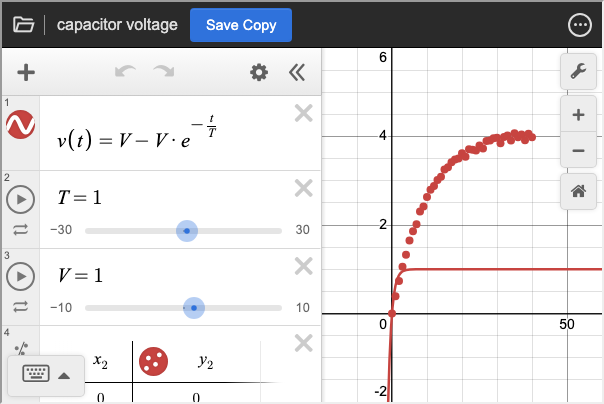
\includegraphics[width=\linewidth]{generated/preview/chargingcircuitgraph-2-preview.png}
\par
\end{sbspanel}%
\begin{sbspanel}{0.21}%
\par
\noindent
\includegraphics[width=\linewidth]{generated/qrcode/chargingcircuitgraph-2.png}
\par
\noindent{}\href{chargingcircuitgraph-2.html}{Standalone}%
\end{sbspanel}%
\end{sidebyside}%
\tcblower
\end{figureptx}%
\par\smallskip%
\noindent\textbf{\blocktitlefont Hint}.\hypertarget{ch5-chargingrccircuits-ex2-2}{}\quad{}Adjust the slider bars until there is good agreement between the fit graph (\(V-V\textrm{e}^{-t/T}\)) and the data in the table.%
\par\smallskip%
\noindent\textbf{\blocktitlefont Answer}.\hypertarget{ch5-chargingrccircuits-ex2-3}{}\quad{}%
\begin{align*}
\tau \amp\approx 9~\textrm{s}\\
v(\infty) \amp\approx 4~\textrm{V}
\end{align*}
%
\end{divisionexercise}%
\begin{divisionexercise}{17}{}{}{ch5-chargingrccircuits-ex1}%
Calculate an expression for \(v(t)\) and \(i(t)\) given the circuit shown in \hyperref[chargingfromzeroendofchapter1]{Figure~{\xreffont\ref{chargingfromzeroendofchapter1}}}. The switch is open for a very long time before closing at a time of zero seconds.%
\begin{figureptx}{Figure}{Circuit diagram corresponding to \hyperlink{ch5-chargingrccircuits-ex1}{Exercise~{\xreffont 5.8.17}}.}{chargingfromzeroendofchapter1}{}%
\begin{image}{0}{1}{0}{}%
\resizebox{\linewidth}{!}{%
\begin{tikzpicture}[font=\sffamily]
	\draw[]	(0,2.5) to [V, l_=20~V]									(0,0);
	\draw[]	(0,2.5) to [R, l^=2~k$\Omega$]							(2.5,2.5);
	\draw[]	(2.5,2.5) to [R, l_=2~k$\Omega$, *-*]					(2.5,0);
	\draw[]	(2.5,2.5) to [cute closing switch]						(4,2.5);
	\draw[]	(4,2.5) to [R, l^=4~k$\Omega$]							(6.5,2.5);
	\draw[]	(6.5,2.5) to [C, l_=5~$\mu$F, v^=$v(t)$, i_=$i(t)$, *-*](6.5,0);
	\draw[]	(6.5,2.5) to [short]									(9.25,2.5);
	\draw[]	(9.25,2.5) to [R, l_=4~k$\Omega$]						(9.25,0);
	\draw[]	(0,0) to [short]										(9.25,0);
\end{tikzpicture}%
}%
\end{image}%
\tcblower
\end{figureptx}%
\par\smallskip%
\noindent\textbf{\blocktitlefont Answer}.\hypertarget{ch5-chargingrccircuits-ex1-2}{}\quad{}%
\begin{align*}
v(t) \amp= 4.44~\textrm{V}\left(1 - \textrm{e}^{-90t}\right)~u(t)\\
i(t) \amp= 2~\textrm{mA}~\textrm{e}^{-90t}~u(t)
\end{align*}
%
\par\smallskip%
\noindent\textbf{\blocktitlefont Solution}.\hypertarget{ch5-chargingrccircuits-ex1-3}{}\quad{}In the initial steady-state, the capacitor will be fully discharged and have an initial voltage of zero. Draw the circuit in the final steady-state. The capacitor can be replaced as an open.%
\begin{figureptx}{Figure}{}{ch5-chargingrccircuits-ex1-3-2}{}%
\begin{image}{0.1}{0.8}{0.1}{}%
\resizebox{\linewidth}{!}{%
\begin{tikzpicture}[font=\sffamily]
	\draw[]	(0,2.5) to [V, l_=20~V]						(0,0);
	\draw[]	(0,2.5) to [R, l^=2~k$\Omega$]				(2.5,2.5);
	\draw[]	(2.5,2.5) to [R, l_=2~k$\Omega$, *-*]		(2.5,0);
	\draw[]	(2.5,2.5) to [R, l^=4~k$\Omega$]			(5,2.5);
	\draw[]	(5,2.5) to [open, v^=$v(\infty)$]			(5,0);
	\draw[]	(5,2.5) to [short]							(7.5,2.5);
	\draw[]	(7.5,2.5) to [R, l_=4~k$\Omega$]			(7.5,0);
	\draw[]	(0,0) to [short]							(7.5,0);
\end{tikzpicture}%
}%
\end{image}%
\tcblower
\end{figureptx}%
Use the voltage divider rule to calculate \(v(\infty)\). (Refer to \hyperref[ch2-voltagedivider-twomesh-example]{Example~{\xreffont\ref{ch2-voltagedivider-twomesh-example}}} for using the voltage divider rule in a two-mesh circuit.)%
\par
%
\begin{align*}
v(\infty) \amp= 20~\textrm{V}\left(\frac{2~\textrm{k}\Omega//(4~\textrm{k}\Omega+4~\textrm{k}\Omega)}{2~\textrm{k}\Omega+2~\textrm{k}\Omega//(4~\textrm{k}\Omega+4~\textrm{k}\Omega)}\right)\left(\frac{4~\textrm{k}\Omega}{8~\textrm{k}\Omega}\right)\\
\amp= 20~\textrm{V}\left(\frac{2~\textrm{k}\Omega//8~\textrm{k}\Omega}{2~\textrm{k}\Omega+2~\textrm{k}\Omega//8~\textrm{k}\Omega}\right)\left(\frac{1}{2}\right)\\
\amp= 20~\textrm{V}\left(\frac{1.6~\textrm{k}\Omega}{3.6~\textrm{k}\Omega}\right)\left(\frac{1}{2}\right)\\
\amp= 4.44~\textrm{V}
\end{align*}
%
\par
Draw the circuit at \(t=0^+\) and deactivate the source to calculate the equivalent resistance as seen by the capacitor.%
\begin{figureptx}{Figure}{}{ch5-chargingrccircuits-ex1-3-6}{}%
\begin{image}{0.1}{0.8}{0.1}{}%
\resizebox{\linewidth}{!}{%
\begin{tikzpicture}[font=\sffamily]
	\draw[]	(0,2.5) to [short]										(0,0);
	\draw[]	(0,2.5) to [R, l^=2~k$\Omega$]							(2.5,2.5);
	\draw[]	(2.5,2.5) to [R, l_=2~k$\Omega$, *-*]					(2.5,0);
	\draw[]	(2.5,2.5) to [R, l^=4~k$\Omega$]						(5,2.5);
	\draw[]	(5,2.5) to [C, l_=5~$\mu$F, v^=$v(t)$, i_=$i(t)$, *-*]	(5,0);
	\draw[]	(5,2.5) to [short]										(7.5,2.5);
	\draw[]	(7.5,2.5) to [R, l_=4~k$\Omega$]						(7.5,0);
	\draw[]	(0,0) to [short]										(7.5,0);
\end{tikzpicture}%
}%
\end{image}%
\tcblower
\end{figureptx}%
Calculate the equivalent resistance as seen by the capacitor.%
\par
%
\begin{align*}
R_{EQ} \amp= (2~\textrm{k}\Omega//2~\textrm{k}\Omega+4~\textrm{k}\Omega)//4~\textrm{k}\Omega\\
\amp= (1~\textrm{k}\Omega+4~\textrm{k}\Omega)//4~\textrm{k}\Omega\\
\amp= 5~\textrm{k}\Omega//4~\textrm{k}\Omega\\
\amp= 2.22~\textrm{k}\Omega
\end{align*}
%
\par
Use \hyperref[ch5-taurcequation]{({\xreffont\ref{ch5-taurcequation}})} to calculate the RC time constant.%
\par
%
\begin{align*}
\tau \amp= RC\\
\amp= (2222~\Omega)\left(5\times10^{-6}~\textrm{F}\right)\\
\amp= 0.011~\textrm{s}
\end{align*}
%
\par
Plug these values into \hyperref[ch5-eqrcchargingvoltage]{({\xreffont\ref{ch5-eqrcchargingvoltage}})} to derive an equation for \(v(t)\).%
\par
%
\begin{equation*}
v(t) = 4.44~\textrm{V}\left(1 - \textrm{e}^{-90t}\right)~u(t)
\end{equation*}
%
\par
Use \hyperref[ch5-rctransientchargingcurrentequation]{({\xreffont\ref{ch5-rctransientchargingcurrentequation}})} to calculate \(i(t)\).%
\par
%
\begin{equation*}
i(t) = 2~\textrm{mA}~\textrm{e}^{-90t}~u(t)
\end{equation*}
%
\end{divisionexercise}%
\begin{divisionexercise}{18}{}{}{ch5-chargingrccircuits-ex3}%
Calculate an expression for \(v(t)\) given the circuit shown in \hyperref[chargingfromzeroendofchapter3]{Figure~{\xreffont\ref{chargingfromzeroendofchapter3}}}. The switch is in position a for a very long time before moving to position b at a time of zero seconds. The circuit parameters are: \(R_1 = 100~\Omega\), \(R_2 = 400~\Omega\), \(C = 20~\textrm{mF}\), and \(V_S = 2~\textrm{V}\). Assume that the op-amp is sufficiently sourced such that the output never saturates.%
\begin{figureptx}{Figure}{Circuit diagram corresponding to \hyperlink{ch5-chargingrccircuits-ex3}{Exercise~{\xreffont 5.8.18}}.}{chargingfromzeroendofchapter3}{}%
\begin{image}{0.1}{0.8}{0.1}{}%
\resizebox{\linewidth}{!}{%
\begin{tikzpicture}[font=\sffamily]
	\draw[]	(0,0) node[op amp] (opamp) {};
	\node[cute spdt up arrow, rotate=180, anchor=in] at ($(opamp.-)-(2.5,0)$) (sw) {};
	\draw[]	(opamp.+) node[ground] {};
	\draw[]	(opamp.-) to [short, *-] ++ (up:1) to [R, l^=$R_2$] ++ (right:2.25) -| (opamp.out);
	\draw[]	($(opamp.-)+(0,1)$) to [short, *-] ++(up:1.25) to [C, l^=$C$] ++ (right:2.25) -| ($(opamp.out)+(0,2)$) to [short, -*] ++(down:0.5);
	\draw[]	(sw.out 1) node[left] {a} to [short] ++ (down:0.1) node[ground] {};
	\draw[]	 (sw.out 2) node[above] {b} to [short] ++(left:1) to [V, l_=$V_S$] ++(down:2.5) node[tlground] {};
	\draw[]	(opamp.-) to [R, l_=$R_1$] ++(left:2.5);
	\draw[]	(opamp.out) to [short, *-] ++ (right:0.5) node[right] {$v(t)$};
\end{tikzpicture}%
}%
\end{image}%
\tcblower
\end{figureptx}%
\par\smallskip%
\noindent\textbf{\blocktitlefont Answer}.\hypertarget{ch5-chargingrccircuits-ex3-2}{}\quad{}%
\begin{equation*}
v(t) = -8~\textrm{V}~\left[1-\textrm{e}^{-0.125t}\right]~u(t)
\end{equation*}
%
\par\smallskip%
\noindent\textbf{\blocktitlefont Solution}.\hypertarget{ch5-chargingrccircuits-ex3-3}{}\quad{}In the initial steady-state, the capacitor will be fully discharged and have an initial voltage of zero. Draw the circuit in the final steady-state. The capacitor can be replaced as an open.%
\begin{figureptx}{Figure}{}{ch5-chargingrccircuits-ex3-3-2}{}%
\begin{image}{0.2}{0.6}{0.2}{}%
\resizebox{\linewidth}{!}{%
\begin{tikzpicture}[font=\sffamily]
	\draw[]	(0,0) node[op amp] (opamp) {};
	\draw[]	(opamp.+) node[ground] {};
	\draw[]	(opamp.-) to [short, *-] ++ (up:1) to [R, l^=$R_2$] ++ (right:2.25) -| (opamp.out);
	\draw[]	 ($(opamp.-)-(2.5,0)$) to [V, l_=$V_S$] ++(down:2.5) node[tlground] {};
	\draw[]	(opamp.-) to [R, l_=$R_1$] ++(left:2.5);
	\draw[]	(opamp.out) to [short, *-] ++ (right:0.5) node[right] {$v(\infty)$};
\end{tikzpicture}%
}%
\end{image}%
\tcblower
\end{figureptx}%
This is an inverting op-amp circuit. Use \hyperref[ch4-invertingopampgaineq]{({\xreffont\ref{ch4-invertingopampgaineq}})} to calculate \(v(\infty)\).%
\par
%
\begin{align*}
v(\infty) \amp= -V_S\frac{R_2}{R_1}\\
\amp= -(2~\textrm{V})\frac{400~\Omega}{100~\Omega}\\
\amp= -8~\textrm{V}
\end{align*}
%
\par
Analyze the circuit at \(t = 0^+\).%
\begin{figureptx}{Figure}{}{ch5-chargingrccircuits-ex3-3-6}{}%
\begin{image}{0.2}{0.6}{0.2}{}%
\resizebox{\linewidth}{!}{%
\begin{tikzpicture}[font=\sffamily]
	\draw[]	(0,0) node[op amp] (opamp) {};
	\draw[]	(opamp.+) node[ground] {};
	\draw[]	(opamp.-) to [short, *-] ++ (up:1) to [R, l^=$R_2$, i^=$I_2$] ++ (right:2.25) -| (opamp.out);
	\draw[]	($(opamp.-)+(0,1)$) to [short, *-] ++(up:1.25) to [C, l^=$C$, i^=$I_3$] ++ (right:2.25) -| ($(opamp.out)+(0,2)$) to [short, -*] ++(down:0.5);
	\draw[]	 ($(opamp.-)-(2.5,0)$) to [V, l_=$V_S$] ++(down:2.5) node[tlground] {};
	\draw[]	($(opamp.-)-(2.5,0)$) to [R, l^=$R_1$, i^=$I_1$] ++(right:2.5);
	\draw[]	(opamp.out) to [short, *-] ++ (right:0.5) node[right] {$v(t)$};
\end{tikzpicture}%
}%
\end{image}%
\tcblower
\end{figureptx}%
Use KCL at the inverting input to obtain a differential equation in terms of \(v(t)\).%
\par
%
\begin{align*}
I_1 \amp = I_2 + I_3\\
\frac{V_S-0}{R_1} \amp= \frac{0-v(t)}{R_2} + C\frac{d}{dt}[0-v(t)]\\
\frac{V_S}{R_1} \amp= \frac{-v(t)}{R_2} + C\frac{d}{dt}[-v(t)]\\
-\frac{V_S}{R_1} \amp= \frac{v(t)}{R_2} + C\frac{dv(t)}{dt}\\
-\frac{V_S}{CR_1} \amp= \frac{dv(t)}{dt} + \frac{v(t)}{CR_2}
\end{align*}
%
\par
Analyze the coefficient \(a_0\) to calculate \(\tau\).%
\par
%
\begin{align*}
\tau \amp= R_2C\\
\amp= (400~\Omega)(0.02~\textrm{F})\\
\amp= 8~\textrm{s}
\end{align*}
%
\par
Use \hyperref[ch5-eqrcchargingvoltage]{({\xreffont\ref{ch5-eqrcchargingvoltage}})} to derive an equation for \(v(t)\).%
\par
%
\begin{align*}
v(t) \amp= v(\infty)\left[1-\textrm{e}^{-\frac{t}{\tau}}\right]~u(t)\\
\amp= -8~\textrm{V}~\left[1-\textrm{e}^{-0.125t}\right]~u(t)
\end{align*}
%
\end{divisionexercise}%
\begin{divisionexercise}{19}{}{}{ch5-generalrccircuits-ex3-actuallycharging4}%
Calculate an expression for \(v(t)\) and \(i(t)\) given the circuit shown in \hyperref[chargingfromzeroendofchapter4]{Figure~{\xreffont\ref{chargingfromzeroendofchapter4}}}. The switch is open for a very long time before closing at a time of zero seconds.%
\begin{figureptx}{Figure}{Circuit diagram corresponding to \hyperlink{ch5-generalrccircuits-ex3-actuallycharging4}{Exercise~{\xreffont 5.8.19}}.}{chargingfromzeroendofchapter4}{}%
\begin{image}{0}{1}{0}{}%
\resizebox{\linewidth}{!}{%
\begin{tikzpicture}[font=\sffamily]
	\draw[]	(0,2.5) to [V, l_=65~V]									(0,0);
	\draw[]	(0,2.5) to [R, l^=30~$\Omega$]							(2.5,2.5);
	\draw[]	(2.5,2.5) to [cute closing switch] 						(5,2.5);
	\draw[]	(5,2.5) to [R, l^=20~$\Omega$]							(7.5,2.5);
	\draw[]	(7.5,2.5) to [C, l_=600~$\mu$F, *-*] 					(7.5,0);
	\draw[]	(7.5,2.5) to [R, l^=40~$\Omega$]						(10,2.5);
	\draw[]	(10,2.5) to [R, l_=100~$\Omega$, v^=$v(t)$, i_=$i(t)$]	(10,0);
	\draw[]	(0,0) to [short]										(10,0);
\end{tikzpicture}%
}%
\end{image}%
\tcblower
\end{figureptx}%
\par\smallskip%
\noindent\textbf{\blocktitlefont Answer}.\hypertarget{ch5-generalrccircuits-ex3-actuallycharging4-2}{}\quad{}%
\begin{align*}
v(t) \amp= 34.2~\textrm{V}~\left[1-\textrm{e}^{-45.2t}\right]~u(t)\\
i(t) \amp= 42~\textrm{mA}~\left[1-\textrm{e}^{-45.2t}\right]~u(t)
\end{align*}
%
\par\smallskip%
\noindent\textbf{\blocktitlefont Solution}.\hypertarget{ch5-generalrccircuits-ex3-actuallycharging4-3}{}\quad{}The capacitor has an initial voltage of 0~V because it is not connected to the source. This will be true of the 100~Ω resistor as well. However, the voltage over a resistor may not be continuous with time. Analyze the circuit at \(t=0^+\) to confirm the value of \(v(0^+)\). Treat the capacitor as a source providing 0~V to the circuit.%
\begin{figureptx}{Figure}{}{ch5-generalrccircuits-ex3-actuallycharging4-3-2}{}%
\begin{image}{0.1}{0.8}{0.1}{}%
\resizebox{\linewidth}{!}{%
\begin{tikzpicture}[font=\sffamily]
	\draw[]	(0,2.5) to [V, l_=65~V]	(0,0);
	\draw[]	(0,2.5) to [R, l^=30~$\Omega$]		(2.5,2.5);
	\draw[]	(2.5,2.5) to [R, l^=20~$\Omega$]		(5,2.5);
	\draw[]	(5,2.5) to [V, l_=0~V, *-*] (5,0);
	\draw[]	(5,2.5) to [R, l^=40~$\Omega$]	(7.5,2.5);
	\draw[]	(7.5,2.5) to [R, l_=100~$\Omega$, v^=$v(0^+)$, i_=$i(0^+)$]	(7.5,0);
	\draw[]	 (0,0) to [short]	(7.5,0);
\end{tikzpicture}%
}%
\end{image}%
\tcblower
\end{figureptx}%
The value of \(v(0^+)\) will also be 0~V (confirm with the voltage divider rule if it's not obvious from observing the circuit diagram).%
\par
Analyze the circuit in its final steady-state configuration to calculate \(v(\infty)\). Treat the capacitor as an open.%
\begin{figureptx}{Figure}{}{ch5-generalrccircuits-ex3-actuallycharging4-3-5}{}%
\begin{image}{0.1}{0.8}{0.1}{}%
\resizebox{\linewidth}{!}{%
\begin{tikzpicture}[font=\sffamily]
	\draw[]	(0,2.5) to [V, l_=65~V]	(0,0);
	\draw[]	(0,2.5) to [R, l^=30~$\Omega$]		(2.5,2.5);
	\draw[]	(2.5,2.5) to [R, l^=20~$\Omega$]		(5,2.5);
	\draw[]	(5,2.5) to [R, l^=40~$\Omega$]	(7.5,2.5);
	\draw[]	(7.5,2.5) to [R, l_=100~$\Omega$, v^=$v(\infty)$, i_=$i(\infty)$]	(7.5,0);
	\draw[]	 (0,0) to [short]	(7.5,0);
\end{tikzpicture}%
}%
\end{image}%
\tcblower
\end{figureptx}%
All of the resistors are in series, therefore, the voltage divider rule can be used to calculate \(v(\infty)\).%
\par
%
\begin{align*}
v(\infty) \amp= (65~\textrm{V})\left(\frac{100~\Omega}{30~\Omega + 20~\Omega + 40~\Omega + 100~\Omega}\right)\\
\amp= (65~\textrm{V})\left(\frac{100~\Omega}{190~\Omega}\right)\\
\amp= (65~\textrm{V})(0.526)\\
\amp= 34.2~\textrm{V}
\end{align*}
%
\par
Analyze the circuit at \(t=0^+\) to calculate the equivalent resistance as seen by the capacitor. (The capacitor will not be treated as a source at this point, as the goal is to calculate equivalent resistance and not voltage.) Deactivate the voltage source by converting it to a short.%
\begin{figureptx}{Figure}{}{ch5-generalrccircuits-ex3-actuallycharging4-3-9}{}%
\begin{image}{0.2}{0.6}{0.2}{}%
\resizebox{\linewidth}{!}{%
\begin{tikzpicture}[font=\sffamily]
	\draw[]	(0,2.5) to [short]	(0,0);
	\draw[]	(0,2.5) to [R, l^=30~$\Omega$]		(2.5,2.5);
	\draw[]	(2.5,2.5) to [R, l^=20~$\Omega$]		(5,2.5);
	\draw[]	(5,2.5) to [C, l_=600~$\mu$F, *-*] (5,0);
	\draw[]	(5,2.5) to [R, l^=40~$\Omega$]	(7.5,2.5);
	\draw[]	(7.5,2.5) to [R, l_=100~$\Omega$]	(7.5,0);
	\draw[]	 (0,0) to [short]	(7.5,0);
\end{tikzpicture}%
}%
\end{image}%
\tcblower
\end{figureptx}%
Combine both sets of series resistors and re-draw the circuit.%
\begin{figureptx}{Figure}{}{ch5-generalrccircuits-ex3-actuallycharging4-3-11}{}%
\begin{image}{0.25}{0.5}{0.25}{}%
\resizebox{\linewidth}{!}{%
\begin{tikzpicture}[font=\sffamily]
	\draw[]	(0,2.5) to [R, l_=50~$\Omega$]	(0,0);
	\draw[]	(0,2.5) to [short]		(5,2.5);
	\draw[]	(2.5,2.5) to [C, l_=600~$\mu$F, *-*] (2.5,0);
	\draw[]	(5,2.5) to [R, l_=140~$\Omega$]	(5,0);
	\draw[]	 (0,0) to [short]	(5,0);
\end{tikzpicture}%
}%
\end{image}%
\tcblower
\end{figureptx}%
The two resistors are in parallel.%
\par
%
\begin{align*}
R_{EQ} \amp= \frac{(50~\Omega)(140~\Omega)}{50~\Omega + 140~\Omega}\\
\amp= \frac{7000~\Omega^2}{190~\Omega}\\
\amp= 36.8~\Omega
\end{align*}
%
\par
Use \hyperref[ch5-taurcequation]{({\xreffont\ref{ch5-taurcequation}})} to calculate \(\tau\).%
\par
%
\begin{align*}
\tau \amp= RC\\
\amp= (36.8~\Omega)(600 \times 10^{-6}~\textrm{F})\\
\amp= 0.022~\textrm{s}
\end{align*}
%
\par
Use \hyperref[ch5-eqrcchargingvoltage]{({\xreffont\ref{ch5-eqrcchargingvoltage}})} to derive an equation for \(v(t)\).%
\par
%
\begin{align*}
v(t) \amp= v(\infty)\left[1-\textrm{e}^{-\frac{t}{\tau}}\right]u(t)\\
\amp= 34.2~\textrm{V}~\left[1-\textrm{e}^{-45.2t}\right]~u(t)
\end{align*}
%
\par
Because the voltage and current are measured over a resistor, Ohm's law will be used to calculate \(i(t)\).%
\par
%
\begin{align*}
i(t) \amp= \frac{v(t)}{R}\\
\amp= \frac{4.2~\textrm{V}~\left[1-\textrm{e}^{-45.2t}\right]~u(t)}{0.1~\textrm{k}\Omega}\\
\amp= 42~\textrm{mA}~\left[1-\textrm{e}^{-45.2t}\right]~u(t)
\end{align*}
%
\end{divisionexercise}%
\begin{divisionexercise}{20}{}{}{ch5-chargingrccircuits-ex5}%
Calculate an expression for \(v(t)\) and \(i(t)\) given the circuit shown in \hyperref[chargingfromzeroendofchapter5]{Figure~{\xreffont\ref{chargingfromzeroendofchapter5}}}. The switch is open for a very long time before closing at a time of zero seconds. The circuit parameters are: \(I_S = 360~\mu\textrm{A}\), \(C = 14~\mu\textrm{F}\), \(k = 2\), \(R_1 = 5~\textrm{k}\Omega\), \(R_2 = 10~\textrm{k}\Omega\), \(R_3 = 2~\textrm{k}\Omega\), and \(R_4 = 3~\textrm{k}\Omega\).%
\begin{figureptx}{Figure}{Circuit diagram corresponding to \hyperlink{ch5-chargingrccircuits-ex5}{Exercise~{\xreffont 5.8.20}}.}{chargingfromzeroendofchapter5}{}%
\begin{image}{0}{1}{0}{}%
\resizebox{\linewidth}{!}{%
\begin{tikzpicture}[font=\sffamily]
	\draw[]	(0,0) to [I, l^=$I_S$]				++(up:2.5);
	\draw[]	(0,2.5) to [short]					++(right:2.5);
	\draw[]	(2.5,2.5) to [R, l_=$R_1$, *-*, v^=$V_X$]	++(down:2.5);
	\draw[]	(2.5,2.5) to [cV, l^=$kV_X$]		++(right:2.5);
	\draw[]	(5,2.5) to [R, l_=$R_3$, *-*]		++(down:2.5);
	\draw[]	(5,2.5) to [cute closing switch]	++(right:2.5);
	\draw[]	(7.5,2.5) to [C, l_=$C$, v^=$v(t)$, i_=$i(t)$, *-*]	++(down:2.5);
	\draw[]	(7.5,2.5) to [short]				++(right:2.5);
	\draw[]	(10,2.5) to [R, l_=$R_4$]			++(down:2.5);
	\draw[]	(0,0) to [short] ++(right:2.5) to [R, l^=$R_2$] ++(right:2.5) to [short]	++(right:5);
\end{tikzpicture}%
}%
\end{image}%
\tcblower
\end{figureptx}%
\par\smallskip%
\noindent\textbf{\blocktitlefont Answer}.\hypertarget{ch5-chargingrccircuits-ex5-2}{}\quad{}%
\begin{align*}
v(t) \amp= -0.348~\textrm{V}~\left[1-\textrm{e}^{-73.8t}\right]~u(t)\\
i(t) \amp= -0.36~\textrm{mA}~\textrm{e}^{-73.8t}~u(t)
\end{align*}
%
\par\smallskip%
\noindent\textbf{\blocktitlefont Solution}.\hypertarget{ch5-chargingrccircuits-ex5-3}{}\quad{}The initial voltage drop over the capacitor will be zero because it is disconnected from any sources. Analyze the circuit in the final steady-state condition to calculate \(v(\infty)\).%
\begin{figureptx}{Figure}{}{ch5-chargingrccircuits-ex5-3-2}{}%
\begin{image}{0}{1}{0}{}%
\resizebox{\linewidth}{!}{%
\begin{tikzpicture}[font=\sffamily]
	\draw[]	(0,0) to [I, l^=$I_S$]	++(up:2.5);
	\draw[]	(0,2.5) to [short]	++(right:2.5);
	\draw[]	(2.5,2.5) to [R, l_=$R_1$, *-*, v^=$V_X$]	++(down:2.5);
	\draw[]	(2.5,2.5) to [cV, l^=$kV_X$]	++(right:2.5);
	\draw[]	(5,2.5) to [R, l_=$R_3$, *-*]	++(down:2.5);
	\draw[]	(5,2.5) to [short]			++(right:5);
	\draw[]	(7.5,2.5) to [open, v^=$v(\infty)$, *-*]	++(down:2.5);
	\draw[]	(10,2.5) to [R, l_=$R_4$]		++(down:2.5);
	\draw[]	(0,0) to [short] ++(right:2.5) to [R, l^=$R_2$] ++(right:2.5) to [short]	++(right:5);
\end{tikzpicture}%
}%
\end{image}%
\tcblower
\end{figureptx}%
Resistors \(R_3\) and \(R_4\) are connected in parallel. The equivalent resistance will be denoted on the circuit diagram symbolically as \(R_X\).%
\par
%
\begin{align*}
R_X \amp= \frac{(2~\textrm{k}\Omega)(3~\textrm{k}\Omega)}{2~\textrm{k}\Omega+3~\textrm{k}\Omega}\\
\amp= 1.2~\textrm{k}\Omega
\end{align*}
%
\begin{figureptx}{Figure}{}{ch5-chargingrccircuits-ex5-3-5}{}%
\begin{image}{0.2}{0.6}{0.2}{}%
\resizebox{\linewidth}{!}{%
\begin{tikzpicture}[font=\sffamily]
	\draw[]	(0,0) to [I, l^=$I_S$]	++(up:2.5);
	\draw[]	(0,2.5) to [short]	++(right:2.5);
	\draw[]	(2.5,2.5) to [R, l_=$R_1$, *-*, v^=$V_X$]	++(down:2.5);
	\draw[]	(2.5,2.5) to [cV, l^=$kV_X$]	++(right:2.5);
	\draw[]	(5,2.5) to [R, l_=$R_X$, v^=$v(\infty)$]	++(down:2.5);
	\draw[]	(0,0) to [short] ++(right:2.5) to [R, l^=$R_2$] ++(right:2.5);
\end{tikzpicture}%
}%
\end{image}%
\tcblower
\end{figureptx}%
Source transformation will not be helpful as it will modify the position of \(V_X\) in the circuit. Superposition is not valid as there is only one independent source. Mesh analysis will therefore be the simplest method for solving this circuit. The circuit is re-drawn below to depict the two mesh currents.%
\begin{figureptx}{Figure}{}{ch5-chargingrccircuits-ex5-3-7}{}%
\begin{image}{0.175}{0.65}{0.175}{}%
\resizebox{\linewidth}{!}{%
\begin{tikzpicture}[font=\sffamily]
	\draw[]	(0,0) to [I, l^=$I_S$]	++(up:3);
	\draw[]	(0,3) to [short]	++(right:3);
	\draw[]	(3,3) to [R, l_=$R_1$, *-*, v^=$V_X$]	++(down:3);
	\draw[]	(3,3) to [cV, l^=$kV_X$]	++(right:3);
	\draw[]	(6,3) to [R, l_=$R_X$, v^=$v(\infty)$]	++(down:3);
	\draw[]	(0,0) to [short] ++(right:3) to [R, l^=$R_2$] ++(right:3);
	\draw[Stealth-] (1.5,1.5)node{$I_A$}  ++(-60:0.5) arc (-60:170:0.5);
	\draw[Stealth-] (4.5,1.5)node{$I_B$}  ++(-60:0.5) arc (-60:170:0.5);
\end{tikzpicture}%
}%
\end{image}%
\tcblower
\end{figureptx}%
Units of kΩ, mA, and V will be used in deriving each mesh analysis equation. Mesh current \(I_A\) is equal to source current \(I_S\). The second equation can be derived by performing KVL around the right-hand mesh. The third equation relates the controlling voltage \(V_X\) to each mesh current.%
\par
%
\begin{align*}
I_A \amp= 0.360\\
5(I_B - I_A) + 2V_X + 1.2I_B + 10I_B \amp= 0\\
5(I_A - I_B) \amp= V_X
\end{align*}
%
\par
The three equations can be expressed in a matrix. The left column contains coefficients of \(I_A\), the middle-left column contains coefficients of \(I_B\), the middle-right column contains coefficients of \(V_X\), and the right column contains constants.%
\par
%
\begin{equation*}
\begin{bmatrix} 
1 	\amp 0	 	\amp 0	 	\amp 0.360\\
-5 	\amp 16.2	\amp 2		\amp 0\\
5	\amp -5		\amp -1		\amp 0
\end{bmatrix}
\end{equation*}
%
\par
The matrix is shown in reduced row echelon form below.%
\par
%
\begin{equation*}
\begin{bmatrix} 
1 	\amp 0 	\amp 0 		\amp 0.360\\
0 	\amp 1 	\amp 0		\amp -0.290\\
0	\amp 0	\amp 1		\amp 3.25
\end{bmatrix}
\end{equation*}
%
\par
Use Ohm's law over \(R_X\) to calculate \(v(\infty)\). The mesh current \(I_B\) is equal to the branch current through that resistor.%
\par
%
\begin{align*}
v(\infty) \amp= (-0.290~\textrm{mA})(1.2~\textrm{k}\Omega)\\
\amp= -0.348~\textrm{V}
\end{align*}
%
\par
There are two methods for deriving \(\tau\). The first is deriving a Thévenin equivalent circuit seen by the capacitor. This circuit is shown below.%
\begin{figureptx}{Figure}{}{ch5-chargingrccircuits-ex5-3-17}{}%
\begin{image}{0.15}{0.7}{0.15}{}%
\resizebox{\linewidth}{!}{%
\begin{tikzpicture}[font=\sffamily]
	\draw[]	(0,0) to [I, l^=$I_S$]	++(up:2.5);
	\draw[]	(0,2.5) to [short]	++(right:2.5);
	\draw[]	(2.5,2.5) to [R, l_=$R_1$, *-*, v^=$V_X$]	++(down:2.5);
	\draw[]	(2.5,2.5) to [cV, l^=$kV_X$]	++(right:2.5);
	\draw[]	(5,2.5) to [R, l_=$R_X$, *-*]	++(down:2.5);
	\draw[]	(0,0) to [short] ++(right:2.5) to [R, l^=$R_2$] ++(right:2.5) to [short, -o] ++(right:2) node[right] {b};
	\draw[]	(5,2.5) to [short, -o]	++(right:2) node[right] {a};
\end{tikzpicture}%
}%
\end{image}%
\tcblower
\end{figureptx}%
The Thévenin equivalent voltage is equal to \(v(\infty)\). Thévenin equivalent resistance cannot be directly calculated due to the presence of a dependent source. Short nodes a and b to calculate the short-circuit current. Note that when nodes a and b are shorted, resistor \(R_X\) is shorted out of the circuit. Mesh analysis is the preferred method to solve for this quantity for the same reasons as above. The short-circuit current will be equal to the mesh current through the right-hand mesh.%
\begin{figureptx}{Figure}{}{ch5-chargingrccircuits-ex5-3-19}{}%
\begin{image}{0.2}{0.6}{0.2}{}%
\resizebox{\linewidth}{!}{%
\begin{tikzpicture}[font=\sffamily]
	\draw[]	(0,0) to [I, l^=$I_S$]	++(up:3);
	\draw[]	(0,3) to [short]	++(right:3);
	\draw[]	(3,3) to [R, l_=$R_1$, *-*, v^=$V_X$]	++(down:3);
	\draw[]	(3,3) to [cV, l^=$kV_X$]	++(right:3);
	\draw[]	(6,3) to [short]	++(down:3);
	\draw[]	(0,0) to [short] ++(right:3) to [R, l^=$R_2$] ++(right:3);
	\draw[Stealth-] (1.5,1.5)node{$I_A$}  ++(-60:0.5) arc (-60:170:0.5);
	\draw[Stealth-] (4.5,1.5)node{$I_{SC}$}  ++(-60:0.5) arc (-60:170:0.5);	
\end{tikzpicture}%
}%
\end{image}%
\tcblower
\end{figureptx}%
Units of kΩ, mA, and V will be used in deriving each mesh analysis equation. Mesh current \(I_A\) is equal to source current \(I_S\). The second equation can be derived by performing KVL around the right-hand mesh. The third equation relates the controlling voltage \(V_X\) to each mesh current.%
\par
%
\begin{align*}
I_A \amp= 0.360\\
5(I_B - I_A) + 2V_X + 10I_B \amp= 0\\
5(I_A - I_B) \amp= V_X
\end{align*}
%
\par
The three equations can be expressed in a matrix. The left column contains coefficients of \(I_A\), the middle-left column contains coefficients of \(I_B\), the middle-right column contains coefficients of \(V_X\), and the right column contains constants.%
\par
%
\begin{equation*}
\begin{bmatrix} 
1 	\amp 0	 	\amp 0	 	\amp 0.360\\
-5 	\amp 15		\amp 2		\amp 0\\
5	\amp -5		\amp -1		\amp 0
\end{bmatrix}
\end{equation*}
%
\par
The matrix is shown in reduced row echelon form below.%
\par
%
\begin{equation*}
\begin{bmatrix} 
1 	\amp 0 	\amp 0 		\amp 0.360\\
0 	\amp 1 	\amp 0		\amp -0.360\\
0	\amp 0	\amp 1		\amp 3.60
\end{bmatrix}
\end{equation*}
%
\par
The short-circuit current is equal to -0.36~mA. Use Ohm's law to calculate the Thévenin equivalent resistance. (The \textquotedblleft{}smell test\textquotedblright{} for this calculation is that both the Thévenin equivalent voltage and short-circuit current values are negative, so the Thévenin equivalent resistance will be positive.) This is equal to the equivalent resistance as seen by the capacitor.%
\par
%
\begin{align*}
R_{TH} \amp= \frac{V_{TH}}{I_{SC}}\\
\amp= \frac{-0.348~\textrm{V}}{-0.36~\textrm{mA}}\\
\amp= 0.967~\textrm{k}\Omega
\end{align*}
%
\par
Use \hyperref[ch5-taurcequation]{({\xreffont\ref{ch5-taurcequation}})} to calculate \(\tau\).%
\par
%
\begin{align*}
\tau \amp= RC\\
\amp= (967~\Omega)(14 \times 10^{-6}~\textrm{F})\\
\amp= 0.014~\textrm{s}
\end{align*}
%
\par
The second method to calculating \(\tau\) is to derive a differential equation for the circuit. This will be done in symbolic form using the diagram shown below. Numerical quantities for each symbolic value will not be plugged in until the very last step of the derivation.%
\begin{figureptx}{Figure}{}{ch5-chargingrccircuits-ex5-3-31}{}%
\begin{image}{0.1}{0.8}{0.1}{}%
\resizebox{\linewidth}{!}{%
\begin{tikzpicture}[font=\sffamily]
	\draw[]	(0,0) to [I, l^=$I_S$]	++(up:2.5);
	\draw[]	(0,2.5) to [short]	++(right:2.5);
	\draw[]	(2.5,2.5) to [R, l_=$R_1$, *-*, v^=$V_X$, i_=$I_1$]	++(down:2.5);
	\draw[]	(2.5,2.5) to [cV, l^=$kV_X$, i>^=$I_2$]	++(right:2.5);
	\draw[]	(5,2.5) to [R, l_=$R_X$, *-*, i_=$I_3$]	++(down:2.5);
	\draw[]	(5,2.5) to [short]			++(right:2.5);
	\draw[]	(7.5,2.5) to [C, l_=$C$, v^=$v(t)$, i_=$i(t)$]	++(down:2.5);
	\draw[]	(0,0) to [short] ++(right:2.5) to [R, l^=$R_2$] ++(right:2.5) to [short]	++(right:2.5);
\end{tikzpicture}%
}%
\end{image}%
\tcblower
\end{figureptx}%
Use KCL to relate each of the branch currents to the source current.%
\par
%
\begin{align}
I_S \amp= I_1 + I_2\label{ch5-chargingrccircuits-ex5-3-33-1-1}\\
I_2 \amp= I_3 + i(t)\label{ch5-lastchargingfromzeroI2}\\
I_S \amp= I_1 + I_3 + i(t)\label{ch5-lastchargingfromzerokcl}
\end{align}
%
\par
Use Ohm's law on each branch to derive the differential equation in terms of \(v(t)\).%
\par
%
\begin{align}
I_1 \amp= \frac{V_X}{R_1}\label{ch5-lastchargingfromzerokvl1}\\
I_3 \amp= \frac{v(t)}{R_X}\label{ch5-lastchargingfromzerokvl2}\\
i(t) \amp= C \frac{dv(t)}{dt}\label{ch5-lastchargingfromzerokvl3}
\end{align}
%
\par
Plug \hyperref[ch5-lastchargingfromzerokvl1]{({\xreffont\ref{ch5-lastchargingfromzerokvl1}})}, \hyperref[ch5-lastchargingfromzerokvl2]{({\xreffont\ref{ch5-lastchargingfromzerokvl2}})}, and \hyperref[ch5-lastchargingfromzerokvl3]{({\xreffont\ref{ch5-lastchargingfromzerokvl3}})} into \hyperref[ch5-lastchargingfromzerokcl]{({\xreffont\ref{ch5-lastchargingfromzerokcl}})}.%
\par
%
\begin{equation}
I_S = \frac{V_X}{R_1} + \frac{v(t)}{R_X} + C \frac{dv(t)}{dt}\label{ch5-lastchargingfromzeroalmostdiffeq}
\end{equation}
%
\par
Use KVL around the center mesh to calculate \(V_X\) in terms of \(v(t)\). Note that the current through \(R_2\) will be equal to \(I_2\). (If you are not convinced of this, consider the relationship between branch and mesh currents in circuit elements in a mesh not shared by other meshes.)%
\par
%
\begin{equation}
V_X = kV_X + v(t) + I_2R_2\label{ch5-lastchargingfromzerovx}
\end{equation}
%
\par
Plug \hyperref[ch5-lastchargingfromzeroI2]{({\xreffont\ref{ch5-lastchargingfromzeroI2}})} into \hyperref[ch5-lastchargingfromzerovx]{({\xreffont\ref{ch5-lastchargingfromzerovx}})} and solve for \(V_X\).%
\par
%
\begin{align}
V_X \amp= kV_X + v(t) + R_2(I_3 + i(t))\label{ch5-chargingrccircuits-ex5-3-41-1-1}\\
\amp= kV_X + v(t) + R_2(\frac{v(t)}{R_X} + C \frac{dv(t)}{dt})\label{ch5-chargingrccircuits-ex5-3-41-1-2}\\
(1-k)V_X \amp= v(t) + \frac{R_2}{R_X}v(t) + R_2C\frac{dv(t)}{dt}\label{ch5-chargingrccircuits-ex5-3-41-1-3}\\
V_X \amp= \left(\frac{1+\frac{R_2}{R_x}}{1-k}\right)v(t) + \left(\frac{R_2C}{1-k}\right)\frac{dv(t)}{dt}\label{ch5-lastcharginfromzerovxsolved}
\end{align}
%
\par
Plug \hyperref[ch5-lastcharginfromzerovxsolved]{({\xreffont\ref{ch5-lastcharginfromzerovxsolved}})} into \hyperref[ch5-lastchargingfromzeroalmostdiffeq]{({\xreffont\ref{ch5-lastchargingfromzeroalmostdiffeq}})} and put into standard form. The last equation contains numerical values. Base units were used to express each quantity.%
\par
%
\begin{align*}
I_S \amp= \frac{1}{R_1}\left[v(t)\left(\frac{1+\frac{R_2}{R_x}}{1-k}\right) + \frac{CR_2}{1-k}\frac{dv(t)}{dt}\right] + \frac{v(t)}{R_X} + C\frac{dv(t)}{dt}\\
\amp= v(t)\left[\frac{1+\frac{R_2}{R_X}}{R_1(1-k)} + \frac{1}{R_X}\right] + \frac{dv(t)}{dt}\left[C + \frac{CR_2}{R_1(1-k)}\right]\\
\amp= v(t)\left[\frac{1+\frac{R_2}{R_X}}{R_1(1-k)} + \frac{1}{R_X}\right] + \frac{dv(t)}{dt}\left[\frac{C(R_1(1-k)+R_2)}{R_1(1-k)}\right]\\
\frac{I_SR_1(1-k)}{C(R_1(1-k)+R_2)} \amp= \frac{dv(t)}{dt} + \left[\frac{1+\frac{R_2}{R_X}}{C(R_1(1-k)+R_2)} + \frac{R_1(1-k)}{R_XC(R_1(1-k)+R_2)}\right]v(t)\\
-25.71 \amp= \frac{dv(t)}{dt} + 73.8v(t)
\end{align*}
%
\par
Calculate \(\tau\) by taking the reciprocal of \(a_0\).%
\par
%
\begin{align*}
\tau \amp= \frac{1}{73.8~\textrm{s}^{-1}}\\
\amp= 0.014~\textrm{s}
\end{align*}
%
\par
This value agrees with the value calculated using the Thévenin equivalence method, as expected.%
\par
Use \hyperref[ch5-eqrcchargingvoltage]{({\xreffont\ref{ch5-eqrcchargingvoltage}})} to derive an equation for \(v(t)\).%
\par
%
\begin{align*}
v(t) \amp= v(\infty)\left[1-\textrm{e}^{-\frac{t}{\tau}}\right]u(t)\\
\amp= -0.348~\textrm{V}~\left[1-\textrm{e}^{-73.8t}\right]~u(t)
\end{align*}
%
\par
Use \hyperref[ch5-rctransientchargingcurrentequation]{({\xreffont\ref{ch5-rctransientchargingcurrentequation}})} to derive an equation for \(i(t)\). Recall that the equivalent resistance as seen by the capacitor is 0.967~kΩ. (If you did not solve for \(\tau\) using the Thévenin equivalence method, use \hyperref[ch5-taurcequation]{({\xreffont\ref{ch5-taurcequation}})} with the value of \(\tau\) derived from the differential equation and solve for \(R\).)%
\par
%
\begin{align*}
i(t) \amp= \frac{v(\infty)}{R}~\textrm{e}^{-\frac{t}{\tau}}~u(t)\\
\amp= \frac{-0.348~\textrm{V}}{0.967~\textrm{k}\Omega}~\textrm{e}^{-73.8t}~u(t)\\
\amp= -0.36~\textrm{mA}~\textrm{e}^{-73.8t}~u(t)
\end{align*}
%
\end{divisionexercise}%
\paragraph{RC Circuits: General Transient Response}\hypertarget{ch5-capacitors-10-6}{}
\begin{divisionexercise}{21}{}{}{ch5-generalrccircuits-ex1}%
Calculate an expression for \(v(t)\) and \(i(t)\) given the circuit shown in \hyperref[generaltransient-endofchapter1]{Figure~{\xreffont\ref{generaltransient-endofchapter1}}}. The switch is open for a very long time before closing at a time of zero seconds.%
\begin{figureptx}{Figure}{Circuit diagram corresponding to \hyperlink{ch5-generalrccircuits-ex1}{Exercise~{\xreffont 5.8.21}}.}{generaltransient-endofchapter1}{}%
\begin{image}{0}{1}{0}{}%
\resizebox{\linewidth}{!}{%
\begin{tikzpicture}[font=\sffamily]
	\draw[]	(0,4) to [V, l_=24~V]									(0,0);
	\draw[]	(0,4) to [R, l^=6~k$\Omega$]							(2.5,4);
	\draw[]	(2.5,4) to [R, l_=1.4~k$\Omega$, *-]					(2.5,2);
	\draw[]	(2.5,2) to [C, l_=40~$\mu$F, v^=$v(t)$, i_=$i(t)$, -*]	(2.5,0);
	\draw[]	(2.5,4) to [short]										(5,4);
	\draw[]	(5,4) to [R, l_=6~k$\Omega$, *-*]						(5,0);
	\draw[]	(5,4) to [cute closing switch]							(7.5,4);
	\draw[]	(7.5,4) to [R, l_=9~k$\Omega$, *-*]						(7.5,0);
	\draw[]	(7.5,4) to [short]										(10,4);
	\draw[]	(10,0) to [I, l^=3.5~mA]								(10,4);
	\draw[]	(0,0) to [short]										(10,0);
\end{tikzpicture}%
}%
\end{image}%
\tcblower
\end{figureptx}%
\par\smallskip%
\noindent\textbf{\blocktitlefont Answer}.\hypertarget{ch5-generalrccircuits-ex1-2}{}\quad{}%
\begin{align*}
v(t) \amp= \left[ 16.875~\textrm{V} - 4.875~\textrm{V}~\textrm{e}^{-6.85t} \right]~u(t) + 12~\textrm{V}~u(-t)\\
i(t) \amp= 1.34~\textrm{mA}~\textrm{e}^{-6.85t}~u(t)
\end{align*}
%
\par\smallskip%
\noindent\textbf{\blocktitlefont Solution}.\hypertarget{ch5-generalrccircuits-ex1-3}{}\quad{}Draw the circuit in the initial steady-state condition. The capacitor can be replaced by an open.%
\begin{figureptx}{Figure}{}{ch5-generalrccircuits-ex1-3-2}{}%
\begin{image}{0.2}{0.6}{0.2}{}%
\resizebox{\linewidth}{!}{%
\begin{tikzpicture}[font=\sffamily]
	\draw[]	(0,4) to [V, l_=24~V]					(0,0);
	\draw[]	(0,4) to [R, l^=6~k$\Omega$]			(2.5,4);
	\draw[]	(2.5,4) to [R, l_=1.4~k$\Omega$, *-]	(2.5,2);
	\draw[]	(2.5,2) to [open, v^=$v(0)$]			(2.5,0);
	\draw[]	(2.5,4) to [short]						(5,4);
	\draw[]	(5,4) to [R, l_=6~k$\Omega$]			(5,0);
	\draw[]	(0,0) to [short]						(5,0);
\end{tikzpicture}%
}%
\end{image}%
\tcblower
\end{figureptx}%
Use the voltage divider rule to calculate \(v(0)\). (Note: the 1.4~kΩ resistor does not contribute to the circuit in this steady-state condition and can be ignored.)%
\par
%
\begin{align*}
v(0) \amp= 24~\textrm{V}\left(\frac{6~\textrm{k}\Omega}{6~\textrm{k}\Omega+6~\textrm{k}\Omega}\right)\\
\amp= 12~\textrm{V}
\end{align*}
%
\par
Draw the circuit in the final steady-state condition. The capacitor can be replaced by an open.%
\begin{figureptx}{Figure}{}{ch5-generalrccircuits-ex1-3-6}{}%
\begin{image}{0}{1}{0}{}%
\resizebox{\linewidth}{!}{%
\begin{tikzpicture}[font=\sffamily]
	\draw[]	(0,4) to [V, l_=24~V]					(0,0);
	\draw[]	(0,4) to [R, l^=6~k$\Omega$]			(2.5,4);
	\draw[]	(2.5,4) to [R, l_=1.4~k$\Omega$, *-]	(2.5,2);
	\draw[]	(2.5,2) to [open, v^=$v(\infty)$]		(2.5,0);
	\draw[]	(2.5,4) to [short]						(5,4);
	\draw[]	(5,4) to [R, l_=6~k$\Omega$, *-*]		(5,0);
	\draw[]	(5,4) to [short]						(7.5,4);
	\draw[]	(7.5,4) to [R, l_=9~k$\Omega$, *-*]		(7.5,0);
	\draw[]	(7.5,4) to [short]						(10,4);
	\draw[]	(10,0) to [I, l^=3.5~mA]				(10,4);
	\draw[]	(0,0) to [short]						(10,0);
\end{tikzpicture}%
}%
\end{image}%
\tcblower
\end{figureptx}%
The 1.4~kΩ resistor does not contribute to the circuit in this steady-state condition and can be removed from the circuit diagram.%
\begin{figureptx}{Figure}{}{ch5-generalrccircuits-ex1-3-8}{}%
\begin{image}{0}{1}{0}{}%
\resizebox{\linewidth}{!}{%
\begin{tikzpicture}[font=\sffamily]
	\draw[]	(0,2.5) to [V, l_=24~V]					(0,0);
	\draw[]	(0,2.5) to [R, l^=6~k$\Omega$]			(2.5,2.5);
	\draw[]	(2.5,2.5) to [open, v^=$v(\infty)$]		(2.5,0);
	\draw[]	(2.5,2.5) to [short]					(5,2.5);
	\draw[]	(5,2.5) to [R, l_=6~k$\Omega$, *-*]		(5,0);
	\draw[]	(5,2.5) to [short]						(7.5,2.5);
	\draw[]	(7.5,2.5) to [R, l_=9~k$\Omega$, *-*]	(7.5,0);
	\draw[]	(7.5,2.5) to [short]					(10,2.5);
	\draw[]	(10,0) to [I, l^=3.5~mA]				(10,2.5);
	\draw[]	(0,0) to [short]						(10,0);
\end{tikzpicture}%
}%
\end{image}%
\tcblower
\end{figureptx}%
Combine the two parallel resistors to simplify the circuit.%
\begin{figureptx}{Figure}{}{ch5-generalrccircuits-ex1-3-10}{}%
\begin{image}{0.1}{0.8}{0.1}{}%
\resizebox{\linewidth}{!}{%
\begin{tikzpicture}[font=\sffamily]
	\draw[]	(0,2.5) to [V, l_=24~V]					(0,0);
	\draw[]	(0,2.5) to [R, l^=6~k$\Omega$]			(2.5,2.5);
	\draw[]	(2.5,2.5) to [open, v^=$v(\infty)$]		(2.5,0);
	\draw[]	(2.5,2.5) to [short]					(5,2.5);
	\draw[]	(5,2.5) to [R, l_=3.6~k$\Omega$, *-*]	(5,0);
	\draw[]	(5,2.5) to [short]						(7.5,2.5);
	\draw[]	(7.5,0) to [I, l^=3.5~mA]				(7.5,2.5);
	\draw[]	(0,0) to [short]						(7.5,0);
\end{tikzpicture}%
}%
\end{image}%
\tcblower
\end{figureptx}%
Transform the 24~V source to a current source. This will cause all circuit elements to be in parallel, simplifying the analysis. The new current source will have a value of%
\par
%
\begin{equation*}
\frac{24~\textrm{V}}{6~\textrm{k}\Omega} = 4~\textrm{mA}.
\end{equation*}
%
\begin{figureptx}{Figure}{}{ch5-generalrccircuits-ex1-3-13}{}%
\begin{image}{0}{1}{0}{}%
\resizebox{\linewidth}{!}{%
\begin{tikzpicture}[font=\sffamily]
	\draw[]	(0,0) to [I, l^=4~mA]					(0,2.5);
	\draw[]	(2.5,2.5) to [R, l_=6~k$\Omega$, *-*]	(2.5,0);
	\draw[]	(5,2.5) to [open, v^=$v(\infty)$]		(5,0);
	\draw[]	(0,2.5) to [short]						(10,2.5);
	\draw[]	(7.5,2.5) to [R, l_=3.6~k$\Omega$, *-*]	(7.5,0);
	\draw[]	(10,0) to [I, l^=3.5~mA]				(10,2.5);
	\draw[]	(0,0) to [short]						(10,0);
\end{tikzpicture}%
}%
\end{image}%
\tcblower
\end{figureptx}%
Combine the two current sources and combine the two parallel resistors.%
\begin{figureptx}{Figure}{}{ch5-generalrccircuits-ex1-3-15}{}%
\begin{image}{0.3}{0.4}{0.3}{}%
\resizebox{\linewidth}{!}{%
\begin{tikzpicture}[font=\sffamily]
	\draw[]	(0,0) to [I, l^=7.5~mA]								(0,2.5);
	\draw[]	(2.5,2.5) to [R, l_=2.25~k$\Omega$, v^=$v(\infty)$]	(2.5,0);
	\draw[]	(0,2.5) to [short]									(2.5,2.5);
	\draw[]	(0,0) to [short]									(2.5,0);
\end{tikzpicture}%
}%
\end{image}%
\tcblower
\end{figureptx}%
Use Ohm's law to calculate \(v(\infty)\).%
\par
%
\begin{align*}
v(\infty) \amp= (7.5~\textrm{mA})(2.25~\textrm{k}\Omega)\\
\amp= 16.875~\textrm{V}
\end{align*}
%
\par
Draw the circuit at \(t=0^+\) and deactivate the sources to calculate the equivalent resistance seen by the capacitor.%
\begin{figureptx}{Figure}{}{ch5-generalrccircuits-ex1-3-19}{}%
\begin{image}{0.1}{0.8}{0.1}{}%
\resizebox{\linewidth}{!}{%
\begin{tikzpicture}[font=\sffamily]
	\draw[]	(0,4) to [short]										(0,0);
	\draw[]	(0,4) to [R, l^=6~k$\Omega$]							(2.5,4);
	\draw[]	(2.5,4) to [R, l_=1.4~k$\Omega$, *-]					(2.5,2);
	\draw[]	(2.5,2) to [C, l_=40~$\mu$F, v^=$v(t)$, i_=$i(t)$, -*]	(2.5,0);
	\draw[]	(2.5,4) to [short]										(5,4);
	\draw[]	(5,4) to [R, l_=6~k$\Omega$, *-*]						(5,0);
	\draw[]	(5,4) to [short]										(7.5,4);
	\draw[]	(7.5,4) to [R, l_=9~k$\Omega$]							(7.5,0);
	\draw[]	(0,0) to [short]										(7.5,0);
\end{tikzpicture}%
}%
\end{image}%
\tcblower
\end{figureptx}%
Calculate the equivalent resistance as seen by the capacitor.%
\par
%
\begin{align*}
R_{EQ} \amp= 9~\textrm{k}\Omega//6~\textrm{k}\Omega//6~\textrm{k}\Omega+1.4~\textrm{k}\Omega\\
\amp= 9~\textrm{k}\Omega//3~\textrm{k}\Omega+1.4~\textrm{k}\Omega\\
\amp= 2.25~\textrm{k}\Omega+1.4~\textrm{k}\Omega\\
\amp= 3.65~\textrm{k}\Omega
\end{align*}
%
\par
Use \hyperref[ch5-taurcequation]{({\xreffont\ref{ch5-taurcequation}})} to calculate the RC time constant.%
\par
%
\begin{align*}
\tau \amp= RC\\
\amp= (3650~\Omega)(40\times10^{-6}~\textrm{F})\\
\amp= 0.146~\textrm{s}
\end{align*}
%
\par
Plug these values into \hyperref[ch5-generaltransientvoltage]{({\xreffont\ref{ch5-generaltransientvoltage}})} to calculate \(v(t)\).%
\par
%
\begin{equation*}
v(t) = \left[ 16.875~\textrm{V} - 4.875~\textrm{V}~\textrm{e}^{-6.85t} \right]~u(t) + 12~\textrm{V}~u(-t)
\end{equation*}
%
\par
Use \hyperref[ch5-generaltransientcurrent]{({\xreffont\ref{ch5-generaltransientcurrent}})} to calculate \(i(t)\).%
\par
%
\begin{equation*}
i(t) = 1.34~\textrm{mA}~\textrm{e}^{-6.85t}~u(t)
\end{equation*}
%
\end{divisionexercise}%
\begin{divisionexercise}{22}{}{}{ch5-generalrccircuits-ex2}%
Calculate an expression for \(v(t)\) and \(i(t)\) given the circuit shown in \hyperref[generalrcendofchatperexamplecircuitquestion2]{Figure~{\xreffont\ref{generalrcendofchatperexamplecircuitquestion2}}}. The switch is closed for a very long time before opening at a time of zero seconds.%
\begin{figureptx}{Figure}{Circuit diagram corresponding to \hyperlink{ch5-generalrccircuits-ex2}{Exercise~{\xreffont 5.8.22}}.}{generalrcendofchatperexamplecircuitquestion2}{}%
\begin{image}{0}{1}{0}{}%
\resizebox{\linewidth}{!}{%
\begin{tikzpicture}[font=\sffamily]
	\draw[]	(0,2.5) to [V, l_=18~V]								(0,0);
	\draw[]	(0,2.5) to [R, l^=10~k$\Omega$]						(2.5,2.5);
	\draw[]	(2.5,2.5) to [cute opening switch]					(4.5,2.5);
	\draw[]	(4.5,2.5) to [R, l_=50~k$\Omega$, *-*]				(4.5,0);
	\draw[]	(4.5,2.5) to [short]								(7,2.5);
	\draw[]	(7,2.5) to [C, l_=40~nF, v^=$v(t)$, i_=$i(t)$, *-*]	(7,0);
	\draw[]	(7,2.5) to [R, l^=25~k$\Omega$]						(9.75,2.5);
	\draw[]	(9.75,2.5) to [R, l_=50~k$\Omega$, *-*]				(9.75,0);
	\draw[]	(9.75,2.5) to [R, l^=50~k$\Omega$]					(12.25,2.5);
	\draw[]	(12.25,2.5) to [V, l_=16~V]							(12.25,0);
	\draw[]	(0,0) to [short]									(12.25,0);
\end{tikzpicture}%
}%
\end{image}%
\tcblower
\end{figureptx}%
\par\smallskip%
\noindent\textbf{\blocktitlefont Answer}.\hypertarget{ch5-generalrccircuits-ex2-2}{}\quad{}%
\begin{align*}
v(t) \amp= \left[ 4~\textrm{V} + 10~\textrm{V}~\textrm{e}^{-1000t}\right]~u(t) + 14~\textrm{V}~u(-t)\\
i(t) \amp= -0.4~\textrm{mA}~\textrm{e}^{-1000t}~u(t)
\end{align*}
%
\par\smallskip%
\noindent\textbf{\blocktitlefont Solution}.\hypertarget{ch5-generalrccircuits-ex2-3}{}\quad{}Draw the circuit in the initial steady-state condition. The capacitor can be replaced by an open.%
\begin{figureptx}{Figure}{}{ch5-generalrccircuits-ex2-3-2}{}%
\begin{image}{0}{1}{0}{}%
\resizebox{\linewidth}{!}{%
\begin{tikzpicture}[font=\sffamily]
	\draw[]	(0,2.5) to [V, l_=18~V]						(0,0);
	\draw[]	(0,2.5) to [R, l^=10~k$\Omega$]				(2.5,2.5);
	\draw[]	(2.5,2.5) to [R, l_=50~k$\Omega$, *-*]		(2.5,0);
	\draw[]	(2.5,2.5) to [short]						(5,2.5);
	\draw[]	(5,2.5) to [open, v^=$v(0)$]				(5,0);
	\draw[]	(5,2.5) to [R, l^=25~k$\Omega$]				(7.5,2.5);
	\draw[]	(7.5,2.5) to [R, l_=50~k$\Omega$, *-*]		(7.5,0);
	\draw[]	(7.5,2.5) to [R, l^=50~k$\Omega$]			(10,2.5);
	\draw[]	(10,2.5) to [V, l_=16~V]					(10,0);
	\draw[]	(0,0) to [short]							(10,0);
\end{tikzpicture}%
}%
\end{image}%
\tcblower
\end{figureptx}%
Convert both sources to current sources. The 18~V source becomes%
\par
%
\begin{equation*}
\frac{18~\textrm{V}}{10~\textrm{k}\Omega} = 1.8~\textrm{mA}.
\end{equation*}
%
\par
The 16~V source becomes%
\par
%
\begin{equation*}
\frac{16~\textrm{V}}{50~\textrm{k}\Omega} = 0.32~\textrm{mA}.
\end{equation*}
%
\begin{figureptx}{Figure}{}{ch5-generalrccircuits-ex2-3-7}{}%
\begin{image}{0}{1}{0}{}%
\resizebox{\linewidth}{!}{%
\begin{tikzpicture}[font=\sffamily]
	\draw[]	(-2.5,0) to [I, l_=1.8~mA]					(-2.5,2.5);
	\draw[]	(0,2.5) to [R, l^=10~k$\Omega$, *-*]		(0,0);
	\draw[]	(2.5,2.5) to [R, l^=50~k$\Omega$, *-*]		(2.5,0);
	\draw[]	(-2.5,2.5) to [short]						(5,2.5);
	\draw[]	(5,2.5) to [open, v^=$v(0)$]				(5,0);
	\draw[]	(5,2.5) to [R, l^=25~k$\Omega$]				(7.5,2.5);
	\draw[]	(7.5,2.5) to [R, l_=50~k$\Omega$, *-*]		(7.5,0);
	\draw[]	(10,2.5) to [R, l_=50~k$\Omega$, *-*]		(10,0);
	\draw[]	(12.5,0) to [I, l^=0.32~mA]					(12.5,2.5);
	\draw[]	(7.5,2.5) to [short]						(12.5,2.5);
	\draw[]	(-2.5,0) to [short]							(12.5,0);
\end{tikzpicture}%
}%
\end{image}%
\tcblower
\end{figureptx}%
Combine the two sets of parallel resistors.%
\begin{figureptx}{Figure}{}{ch5-generalrccircuits-ex2-3-9}{}%
\begin{image}{0}{1}{0}{}%
\resizebox{\linewidth}{!}{%
\begin{tikzpicture}[font=\sffamily]
	\draw[]	(0,0) to [I, l^=1.8~mA]						(0,2.5);
	\draw[]	(2.5,2.5) to [R, l_=8.33~k$\Omega$, *-*]	(2.5,0);
	\draw[]	(0,2.5) to [short]							(5,2.5);
	\draw[]	(5,2.5) to [open, v^=$v(0)$]				(5,0);
	\draw[]	(5,2.5) to [R, l^=25~k$\Omega$]				(7.5,2.5);
	\draw[]	(7.5,2.5) to [R, l_=25~k$\Omega$, *-*]		(7.5,0);
	\draw[]	(10,0) to [I, l^=0.32~mA]					(10,2.5);
	\draw[]	(7.5,2.5) to [short]						(10,2.5);
	\draw[]	(0,0) to [short]							(10,0);
\end{tikzpicture}%
}%
\end{image}%
\tcblower
\end{figureptx}%
Convert the 0.32~mA source to a voltage source. The voltage becomes%
\par
%
\begin{equation*}
(0.32~\textrm{mA})(25~\textrm{k}\Omega) = 8~\textrm{V}.
\end{equation*}
%
\begin{figureptx}{Figure}{}{ch5-generalrccircuits-ex2-3-12}{}%
\begin{image}{0}{1}{0}{}%
\resizebox{\linewidth}{!}{%
\begin{tikzpicture}[font=\sffamily]
	\draw[]	(0,0) to [I, l^=1.8~mA]						(0,2.5);
	\draw[]	(2.5,2.5) to [R, l_=8.33~k$\Omega$, *-*]	(2.5,0);
	\draw[]	(0,2.5) to [short]							(5,2.5);
	\draw[]	(5,2.5) to [open, v^=$v(0)$]				(5,0);
	\draw[]	(5,2.5) to [R, l^=25~k$\Omega$]				(7.5,2.5);
	\draw[]	(7.5,2.5) to [R, l^=25~k$\Omega$]			(10,2.5);
	\draw[]	(10,2.5) to [V, l_=8~V]						(10,0);
	\draw[]	(0,0) to [short]							(10,0);
\end{tikzpicture}%
}%
\end{image}%
\tcblower
\end{figureptx}%
Combine the two series resistors.%
\begin{figureptx}{Figure}{}{ch5-generalrccircuits-ex2-3-14}{}%
\begin{image}{0.1}{0.8}{0.1}{}%
\resizebox{\linewidth}{!}{%
\begin{tikzpicture}[font=\sffamily]
	\draw[]	(0,0) to [I, l^=1.8~mA]					(0,2.5);
	\draw[]	(2.5,2.5) to [R, l_=8.33~k$\Omega$, *-*]		(2.5,0);
	\draw[]	(0,2.5) to [short]						(5,2.5);
	\draw[]	(5,2.5) to [open, v^=$v(0)$]				(5,0);
	\draw[]	(5,2.5) to [R, l^=50~k$\Omega$]			(7.5,2.5);
	\draw[]	(7.5,2.5) to [V, l_=8~V]					(7.5,0);
	\draw[]	(0,0) to [short]							(7.5,0);
\end{tikzpicture}%
}%
\end{image}%
\tcblower
\end{figureptx}%
Convert the voltage source to a current source. The value of the current source is%
\par
%
\begin{equation*}
\frac{8~\textrm{V}}{50~\textrm{k}\Omega} = 0.16~\textrm{mA}.
\end{equation*}
%
\begin{figureptx}{Figure}{}{ch5-generalrccircuits-ex2-3-17}{}%
\begin{image}{0}{1}{0}{}%
\resizebox{\linewidth}{!}{%
\begin{tikzpicture}[font=\sffamily]
	\draw[]	(0,0) to [I, l^=1.8~mA]						(0,2.5);
	\draw[]	(2.5,2.5) to [R, l_=8.33~k$\Omega$, *-*]	(2.5,0);
	\draw[]	(0,2.5) to [short]							(10,2.5);
	\draw[]	(5,2.5) to [open, v^=$v(0)$]				(5,0);
	\draw[]	(7.5,2.5) to [R, l_=50~k$\Omega$, *-*]		(7.5,0);
	\draw[]	(10,0) to [I, l_=0.16~mA]					(10,2.5);
	\draw[]	(0,0) to [short]							(10,0);
\end{tikzpicture}%
}%
\end{image}%
\tcblower
\end{figureptx}%
Combine the two sources and combine the two parallel resistors.%
\begin{figureptx}{Figure}{}{ch5-generalrccircuits-ex2-3-19}{}%
\begin{image}{0.3}{0.4}{0.3}{}%
\resizebox{\linewidth}{!}{%
\begin{tikzpicture}[font=\sffamily]
	\draw[]	(0,0) to [I, l^=1.96~mA]						(0,2.5);
	\draw[]	(2.5,2.5) to [R, l_=7.14~k$\Omega$, v^=$v(0)$]	(2.5,0);
	\draw[]	(0,2.5) to [short]								(2.5,2.5);
	\draw[]	(0,0) to [short]								(2.5,0);
\end{tikzpicture}%
}%
\end{image}%
\tcblower
\end{figureptx}%
Use Ohm's law to calculate \(v(0)\).%
\par
%
\begin{align*}
v(0) \amp= (1.96~\textrm{mA})(7.14~\textrm{k}\Omega)\\
\amp= 14~\textrm{V}
\end{align*}
%
\par
Draw the circuit in the final steady-state condition. The capacitor can be replaced by an open.%
\begin{figureptx}{Figure}{}{ch5-generalrccircuits-ex2-3-23}{}%
\begin{image}{0.1}{0.8}{0.1}{}%
\resizebox{\linewidth}{!}{%
\begin{tikzpicture}[font=\sffamily]
	\draw[]	(4.5,2.5) to [R, l_=50~k$\Omega$]			(4.5,0);
	\draw[]	(4.5,2.5) to [short]						(7,2.5);
	\draw[]	(7,2.5) to [open, v^=$v(\infty)$]			(7,0);
	\draw[]	(7,2.5) to [R, l^=25~k$\Omega$]				(9.75,2.5);
	\draw[]	(9.75,2.5) to [R, l_=50~k$\Omega$, *-*]		(9.75,0);
	\draw[]	(9.75,2.5) to [R, l^=50~k$\Omega$]			(12.25,2.5);
	\draw[]	(12.25,2.5) to [V, l_=16~V]					(12.25,0);
	\draw[]	(4.5,0) to [short]							(12.25,0);
\end{tikzpicture}%
}%
\end{image}%
\tcblower
\end{figureptx}%
Use the voltage divider rule to calculate \(v(\infty)\). (Refer to \hyperref[ch2-voltagedivider-twomesh-example]{Example~{\xreffont\ref{ch2-voltagedivider-twomesh-example}}} for using the voltage divider rule in a two-mesh circuit.)%
\par
%
\begin{align*}
v(\infty) \amp= 16~\textrm{V}\left(\frac{50~\textrm{k}\Omega//75~\textrm{k}\Omega}{50~\textrm{k}\Omega+50~\textrm{k}\Omega//75~\textrm{k}\Omega}\right)\left(\frac{50~\textrm{k}\Omega}{75~\textrm{k}\Omega}\right)\\
\amp= 16~\textrm{V}\left(\frac{30~\textrm{k}\Omega}{50~\textrm{k}\Omega+30~\textrm{k}\Omega}\right)\left(\frac{2}{3}\right)\\
\amp= 4~\textrm{V}
\end{align*}
%
\par
Draw the circuit at \(t=0^+\) and deactivate the source to calculate the equivalent resistance seen by the capacitor.%
\begin{figureptx}{Figure}{}{ch5-generalrccircuits-ex2-3-27}{}%
\begin{image}{0.1}{0.8}{0.1}{}%
\resizebox{\linewidth}{!}{%
\begin{tikzpicture}[font=\sffamily]
	\draw[]	(4.5,2.5) to [R, l_=50~k$\Omega$]					(4.5,0);
	\draw[]	(4.5,2.5) to [short]								(7,2.5);
	\draw[]	(7,2.5) to [C, l_=40~nF, v^=$v(t)$, i_=$i(t)$, *-*]	(7,0);
	\draw[]	(7,2.5) to [R, l^=25~k$\Omega$]						(9.75,2.5);
	\draw[]	(9.75,2.5) to [R, l_=50~k$\Omega$, *-*]				(9.75,0);
	\draw[]	(9.75,2.5) to [R, l^=50~k$\Omega$]					(12.25,2.5);
	\draw[]	(12.25,2.5) to [short]								(12.25,0);
	\draw[]	(4.5,0) to [short]									(12.25,0);
\end{tikzpicture}%
}%
\end{image}%
\tcblower
\end{figureptx}%
Calculate the equivalent resistance as seen by the capacitor.%
\par
%
\begin{align*}
R_{EQ} \amp= (50~\textrm{k}\Omega//50~\textrm{k}\Omega+25~\textrm{k}\Omega)//50~\textrm{k}\Omega\\
\amp= (25~\textrm{k}\Omega+25~\textrm{k}\Omega)//50~\textrm{k}\Omega\\
\amp= 50~\textrm{k}\Omega//50~\textrm{k}\Omega\\
\amp= 25~\textrm{k}\Omega
\end{align*}
%
\par
Use \hyperref[ch5-taurcequation]{({\xreffont\ref{ch5-taurcequation}})} to calculate the RC time constant.%
\par
%
\begin{align*}
\tau \amp= RC\\
\amp= (25000~\Omega)(40\times10^{-9}\textrm{F})\\
\amp= 0.001~\textrm{s}
\end{align*}
%
\par
Plug these values into \hyperref[ch5-generaltransientvoltage]{({\xreffont\ref{ch5-generaltransientvoltage}})} to derive \(v(t)\).%
\par
%
\begin{equation*}
v(t) = \left[ 4~\textrm{V} + 10~\textrm{V}~\textrm{e}^{-1000t}\right]~u(t) + 14~\textrm{V}~u(-t)
\end{equation*}
%
\par
Use \hyperref[ch5-generaltransientcurrent]{({\xreffont\ref{ch5-generaltransientcurrent}})} to calculate \(i(t)\).%
\par
%
\begin{equation*}
i(t) = -0.4~\textrm{mA}~\textrm{e}^{-1000t}~u(t)
\end{equation*}
%
\end{divisionexercise}%
\begin{divisionexercise}{23}{}{}{ch5-chargingrccircuits-ex4}%
Derive equations for \(v(t)\) and \(i(t)\) for the circuit shown in \hyperref[chargingfromzerocircuitexample1]{Figure~{\xreffont\ref{chargingfromzerocircuitexample1}}}. The switch is open for a very long time before closing at a time of zero seconds.%
\begin{figureptx}{Figure}{Circuit diagram corresponding to \hyperlink{ch5-chargingrccircuits-ex4}{Exercise~{\xreffont 5.8.23}}.}{chargingfromzerocircuitexample1}{}%
\begin{image}{0.2}{0.6}{0.2}{}%
\resizebox{\linewidth}{!}{%
\begin{tikzpicture}[font=\sffamily]
	\draw[]	(0,2.5) to [V, l_=40~mV]							(0,0);
	\draw[]	(0,2.5) to [cute closing switch] 					(2.5,2.5);
	\draw[]	(2.5,2.5) to [R, l^=2~$\Omega$, *-*]				(5,2.5);
	\draw[]	(2.5,2.5) --++ (up:1.5) to [C, l^=120~nF] 			++ (right:2.5) --++ (down:1.5);
	\draw[]	(5,2.5) to [R, l_=4~$\Omega$, v^=$v(t)$, i_=$i(t)$]	(5,0);
	\draw[]	 (0,0) to [short]									(5,0);
\end{tikzpicture}%
}%
\end{image}%
\tcblower
\end{figureptx}%
\par\smallskip%
\noindent\textbf{\blocktitlefont Answer}.\hypertarget{ch5-chargingrccircuits-ex4-2}{}\quad{}%
\begin{align*}
v(t) \amp= \left[26.7~\textrm{mV} + 13.3~\textrm{mV}~\textrm{e}^{-6250000t} \right] u(t)\\
i(t) \amp= \left[6.67~\textrm{mA} + 3.33~\textrm{mA}~\textrm{e}^{-6250000t} \right] u(t)
\end{align*}
%
\par\smallskip%
\noindent\textbf{\blocktitlefont Solution}.\hypertarget{ch5-chargingrccircuits-ex4-3}{}\quad{}The capacitor has an initial voltage of 0~V. This value must be continuous with time (i.e. \(v_C(0^-) = v_C(0^+) = 0~\textrm{V}\)). The resistor will have an initial voltage of 0~V as well (due to not being connected to the source), but this value may not be continuous with time. To calculate \(v(0^+)\), analyze the circuit at \(t=0^+\). Treat the capacitor as a source providing \(v_C(0)\) volts.%
\begin{figureptx}{Figure}{}{ch5-chargingrccircuits-ex4-3-2}{}%
\begin{image}{0.2}{0.6}{0.2}{}%
\resizebox{\linewidth}{!}{%
\begin{tikzpicture}[font=\sffamily]
	\draw[]	(0,2.5) to [V, l_=40~mV]	(0,0);
	\draw[]	(0,2.5) to [short] (2.5,2.5);
	\draw[]	(2.5,2.5) to [R, l^=2~$\Omega$, *-*]		(5,2.5);
	\draw[]	(2.5,2.5) --++ (up:1.5) to [V, l^=0~V] ++ (right:2.5) --++ (down:1.5);
	\draw[]	(5,2.5) to [R, l_=4~$\Omega$, v^=$v(0^+)$, i_=$i(0^+)$]	(5,0);
	\draw[]	 (0,0) to [short]	(5,0);
\end{tikzpicture}%
}%
\end{image}%
\tcblower
\end{figureptx}%
No voltage drops over the 2~Ω resistor (this is due to KVL; it is in parallel with a 0~V source and therefore must have the same voltage drop). Therefore, all 40~mV provided by the source must be dropped over the 4~Ω resistor.%
\par
Now analyze the circuit at \(t=0^+\) to calculate the equivalent resistance as seen by the capacitor. (The capacitor will not be treated as a source at this point, as the goal is to calculate equivalent resistance and not voltage.) Deactivate the 40~mV voltage source by converting it to a short.%
\begin{figureptx}{Figure}{}{ch5-chargingrccircuits-ex4-3-5}{}%
\begin{image}{0.35}{0.3}{0.35}{}%
\resizebox{\linewidth}{!}{%
\begin{tikzpicture}[font=\sffamily]
	\draw[]	(0,2.5) to [short]	(0,0);
	\draw[]	(0,2.5) to [R, l^=2~$\Omega$, *-*]		(2.5,2.5);
	\draw[]	(0,2.5) --++ (up:1.5) to [C, l^=120~nF] ++ (right:2.5) --++ (down:1.5);
	\draw[]	(2.5,2.5) to [R, l_=4~$\Omega$]	(2.5,0);
	\draw[]	 (0,0) to [short]	(2.5,0);
\end{tikzpicture}%
}%
\end{image}%
\tcblower
\end{figureptx}%
The two resistors are in parallel. Calculate the equivalent resistance.%
\par
%
\begin{align*}
R_{EQ} \amp= \frac{(2~\Omega)(4~\Omega)}{2~\Omega + 4~\Omega}\\
\amp= \frac{8~\Omega^2}{6~\Omega}\\
\amp= 1.33~\Omega
\end{align*}
%
\par
Use \hyperref[ch5-taurcequation]{({\xreffont\ref{ch5-taurcequation}})} to calculate \(\tau\).%
\par
%
\begin{align*}
\tau \amp= RC\\
\amp= (1.33~\Omega)(120 \times 10^{-9}~\textrm{F})\\
\amp= 1.6 \times 10^{-7}~\textrm{s}
\end{align*}
%
\par
Analyze the circuit in the final steady-state to calculate \(v(\infty)\). Treat the capacitor as an open circuit.%
\begin{figureptx}{Figure}{}{ch5-chargingrccircuits-ex4-3-11}{}%
\begin{image}{0.3}{0.4}{0.3}{}%
\resizebox{\linewidth}{!}{%
\begin{tikzpicture}[font=\sffamily]
	\draw[]	(0,2.5) to [V, l_=40~mV]	(0,0);
	\draw[]	(0,2.5) to [R, l^=2~$\Omega$]		(2.5,2.5);
	\draw[]	(2.5,2.5) to [R, l_=4~$\Omega$, v^=$v(\infty)$, i_=$i(\infty)$]	(2.5,0);
	\draw[]	 (0,0) to [short]	(2.5,0);
\end{tikzpicture}%
}%
\end{image}%
\tcblower
\end{figureptx}%
Use the voltage divider rule to calculate \(v(\infty)\).%
\par
%
\begin{align*}
v(\infty) \amp= (40~\textrm{mV})\left(\frac{4~\Omega}{2~\Omega + 4~\Omega}\right)\\
\amp= (40~\textrm{mV})(0.667)\\
\amp= 26.7~\textrm{mV}
\end{align*}
%
\par
Use \hyperref[ch5-generaltransientvoltage]{({\xreffont\ref{ch5-generaltransientvoltage}})} to derive an equation for \(v(t)\).%
\par
%
\begin{align*}
v(t) \amp= \left[v(\infty) + \left( v(0^+) - v(\infty) \right) \textrm{e}^{-\frac{t}{\tau}} \right] u(t) + v(0^-)u(-t)\\
\amp= \left[26.7~\textrm{mV} + 13.3~\textrm{mV}~\textrm{e}^{-6250000t} \right] u(t)
\end{align*}
%
\par
Because the voltage and current are measured over a resistor, Ohm's law will be used to calculate \(i(t)\).%
\par
%
\begin{align*}
i(t) \amp= \frac{v(t)}{R}\\
\amp = \frac{\left[26.7~\textrm{mV} + 13.3~\textrm{mV}~\textrm{e}^{-6250000t} \right] u(t)}{4~\Omega}\\
\amp= \left[6.67~\textrm{mA} + 3.33~\textrm{mA}~\textrm{e}^{-6250000t} \right] u(t)
\end{align*}
%
\end{divisionexercise}%
\begin{divisionexercise}{24}{}{}{ch5-generalrccircuits-ex4}%
Derive equations for \(v(t)\) and \(i(t)\) for the circuit shown in \hyperref[generalrccircuitexamplecircuit4]{Figure~{\xreffont\ref{generalrccircuitexamplecircuit4}}}. The switch is in position a for a very long time before moving to position b at a time of zero seconds. The switch then moves to position c at a time of 15~ms and remains in that position for a long time. Assume that the op-amp is sufficiently sourced such that the output will never saturate.%
\begin{figureptx}{Figure}{Circuit diagram corresponding to \hyperlink{ch5-generalrccircuits-ex4}{Exercise~{\xreffont 5.8.24}}.}{generalrccircuitexamplecircuit4}{}%
\begin{image}{0}{1}{0}{}%
\resizebox{\linewidth}{!}{%
\begin{tikzpicture}[font=\sffamily]
	\draw[]	(0,0) node [op amp] (opamp) {};
	\draw[]	(opamp.-) to [short, *-] ++(left:0.5);
	\node[ground]	at (opamp.+) {};
	\node[cute spdt down, rotate=145, anchor=in]	at ($(opamp.-)-(0.5,0)$) (sw) {};
	\node[ocirc]	at ($(sw.out 2)-(0,1.45)$) (sw3) {};
	\draw[]	(sw.out 2) node[above left] {a} --++ (up:0.5) to [R, l_=1~k$\Omega$]	++(left:5.5) to [V, l_=5~V] ++(down:2.5) node[tlground] {};
	\draw[]	(sw.out 1) node[above] {b} to [R, l_=1~k$\Omega$]	++(left:3.5) to [V, l_=2~V] ++(down:2.5) node[tlground] {};
	\draw[]	(sw3) node[above] {c} --++ (down:0.5) to [R, l_=1~k$\Omega$]	++(left:2.5) to [V, l_=1~V] ++(down:2.5) node[tlground] {};
	\draw[]	(opamp.-) to [short, -*] ++(up:1.25) to [R, l^=2~k$\Omega$]	++(right:2.25) -| (opamp.out);
	\draw[]	($(opamp.-)+(0,1.25)$) --++ (up:1.25) to [C, l^=10~$\mu$F]	++(right:2.38) to [short, -*] ++(down:1.25);
	\draw[]	(opamp.out) to [short, *-o]	++(right:1) node[right] {$v(t)$};
	\draw[]	($(opamp.out)+(0.5,0)$) to [R, l_=100~k$\Omega$, i^=$i(t)$, *-] ++(down:2.5) node[tlground] {};
\end{tikzpicture}%
}%
\end{image}%
\tcblower
\end{figureptx}%
\par\smallskip%
\noindent\textbf{\blocktitlefont Answer}.\hypertarget{ch5-generalrccircuits-ex4-2}{}\quad{}%
\begin{align*}
v(t) \amp= -10~\textrm{V} + \left[-4~\textrm{V}-6~\textrm{V}~\textrm{e}^{-50t}\right]~u(t) - \left[-4~\textrm{V} - 2.83~\textrm{V}~\textrm{e}^{-50(t-0.015)}\right]~u(t-0.015) + \left[-2~\textrm{V} - 4.83~\textrm{V}~\textrm{e}^{-50(t-0.015)}\right]~u(t-0.015)\\
i(t) \amp= -0.1~\textrm{mA} + \left[-0.04~\textrm{mA}-0.06~\textrm{mA}~\textrm{e}^{-50t}\right]~u(t) - \left[-0.04~\textrm{mA} - 0.0283~\textrm{mA}~\textrm{e}^{-50(t-0.015)}\right]~u(t-0.015) + \left[-0.02~\textrm{mA} - 0.0483~\textrm{mA}~\textrm{e}^{-50(t-0.015)}\right]~u(t-0.015)
\end{align*}
%
\par\smallskip%
\noindent\textbf{\blocktitlefont Solution}.\hypertarget{ch5-generalrccircuits-ex4-3}{}\quad{}First, analyze the circuit in its initial condition to calculate \(v(0)\). The switch is in position a and the capacitor acts as an open circuit. Only the 5~V source is connected in this configuration.%
\begin{figureptx}{Figure}{}{ch5-generalrccircuits-ex4-3-2}{}%
\begin{image}{0.2}{0.6}{0.2}{}%
\resizebox{\linewidth}{!}{%
\begin{tikzpicture}[font=\sffamily]
	\draw[]	(0,0) node [op amp] (opamp) {};
	\draw[]	(opamp.-) to [short, *-] ++(left:0.5);
	\node[ground]	at (opamp.+) {};
	\draw[]	(opamp.-) to [R, l_=1~k$\Omega$, *-]	++(left:2.5) to [V, l_=5~V] ++(down:2.5) node[tlground] {};
	\draw[]	(opamp.-) to [short] ++(up:1.25) to [R, l^=2~k$\Omega$]	++(right:2.25) -| (opamp.out);
	\draw[]	(opamp.out) to [short, *-o]	++(right:1) node[right] {$v(0)$};
	\draw[]	($(opamp.out)+(0.5,0)$) to [R, l_=100~k$\Omega$, i^=$i(0)$, *-] ++(down:2.5) node[tlground] {};
\end{tikzpicture}%
}%
\end{image}%
\tcblower
\end{figureptx}%
The circuit is an inverting op-amp. Use \hyperref[ch4-invertingopampgaineq]{({\xreffont\ref{ch4-invertingopampgaineq}})} to calculate \(v(0)\).%
\par
%
\begin{align*}
v(0) \amp= -(5~\textrm{V})\left(\frac{2~\textrm{k}\Omega}{1~\textrm{k}\Omega}\right)\\
\amp= -10~\textrm{V}
\end{align*}
%
\par
This means that the equation for \(v(t)\) will contain a term of \(-10~\textrm{V}~u(-t)\), representing the initial steady-state conditions of the circuit. This creates a \(v(t)\) graph that so far appears as follows.%
\begin{figureptx}{Figure}{}{ch5-generalrccircuits-ex4-3-6}{}%
\begin{image}{0}{1}{0}{}%
\resizebox{\linewidth}{!}{%
\begin{tikzpicture}[font=\sffamily]
	\begin{axis}[ylabel={$v(t)$~(V)}, xlabel={$t$~(ms)}, width=\linewidth, height=5cm, xmin=-5, xmax=50, ymin=-15, ymax=0, ytick={-15,-10,...,0}]
		\addplot[black, thick] coordinates {(-5,-10) (0,-10)};
				\end{axis}
\end{tikzpicture}%
}%
\end{image}%
\tcblower
\end{figureptx}%
Analyze the circuit with the switch in position b to determine how the circuit will act between 0~ms and 15~ms. Only the 2~V source is connected in this configuration.%
\begin{figureptx}{Figure}{}{ch5-generalrccircuits-ex4-3-8}{}%
\begin{image}{0.2}{0.6}{0.2}{}%
\resizebox{\linewidth}{!}{%
\begin{tikzpicture}[font=\sffamily]
	\draw[]	(0,0) node [op amp] (opamp) {};
	\draw[]	(opamp.-) to [short, *-] ++(left:0.5);
	\node[ground]	at (opamp.+) {};
	\draw[]	(opamp.-) to [R, l_=1~k$\Omega$]	++(left:2.5) to [V, l_=2~V] ++(down:2.5) node[tlground] {};
	\draw[]	(opamp.-) to [short, -*] ++(up:1.25) to [R, l^=2~k$\Omega$]	++(right:2.25) -| (opamp.out);
	\draw[]	($(opamp.-)+(0,1.25)$) --++ (up:1.25) to [C, l^=10~$\mu$F]	++(right:2.38) to [short, -*] ++(down:1.25);
	\draw[]	(opamp.out) to [short, *-o]	++(right:1) node[right] {$v(t)$};
	\draw[]	($(opamp.out)+(0.5,0)$) to [R, l_=100~k$\Omega$, i^=$i(t)$, *-] ++(down:2.5) node[tlground] {};
\end{tikzpicture}%
}%
\end{image}%
\tcblower
\end{figureptx}%
Derive a differential equation to calculate \(\tau\). To derive this symbolically, the voltage source will be referred to as \(V_S\), the 1~kΩ resistor will be referred to as \(R_1\), the 2~kΩ resistor will be referred to as \(R_2\), the 100~kΩ resistor will be referred to as \(R_3\), and the capacitor will be referred to as \(C\). Use KCL at the inverting node of the op-amp to derive the differential equation.%
\par
%
\begin{align*}
\frac{V_S}{R_1} \amp= \frac{0-v(t)}{R_2} + C \frac{d}{dt}\left(0-v(t)\right)\\
\amp= -\frac{v(t)}{R_2} - C\frac{dv(t)}{dt}\\
-\frac{V_S}{CR_1} \amp= \frac{dv(t)}{dt} + \frac{1}{CR_2}v(t)
\end{align*}
%
\par
Use coefficient \(a_0\) to calculate \(\tau\).%
\par
%
\begin{align*}
\tau \amp= \frac{1}{a_0}\\
\amp= CR_2\\
\amp= (10 \times 10^{-6}~\textrm{F})(2000~\Omega)\\
\amp= 0.02~\textrm{s}
\end{align*}
%
\par
Note that because the coefficient \(a_0\) in the differential equation is only a function of the 2~kΩ resistor, the value of \(\tau\) will not change based on the position of the switch.%
\par
Calculate the value of \(v(\infty_b)\), which is the output voltage that would occur if the switch were to remain in position b for a very long time. The capacitor acts as an open.%
\begin{figureptx}{Figure}{}{ch5-generalrccircuits-ex4-3-15}{}%
\begin{image}{0.2}{0.6}{0.2}{}%
\resizebox{\linewidth}{!}{%
\begin{tikzpicture}[font=\sffamily]
	\draw[]	(0,0) node [op amp] (opamp) {};
	\draw[]	(opamp.-) to [short, *-] ++(left:0.5);
	\node[ground]	at (opamp.+) {};
	\draw[]	(opamp.-) to [R, l_=1~k$\Omega$]	++(left:2.5) to [V, l_=2~V] ++(down:2.5) node[tlground] {};
	\draw[]	(opamp.-) to [short] ++(up:1.25) to [R, l^=2~k$\Omega$]	++(right:2.25) -| (opamp.out);
	\draw[]	(opamp.out) to [short, *-o]	++(right:1) node[right] {$v(\infty_b)$};
	\draw[]	($(opamp.out)+(0.5,0)$) to [R, l_=100~k$\Omega$, i^=$i(\infty_b)$, *-] ++(down:2.5) node[tlground] {};
\end{tikzpicture}%
}%
\end{image}%
\tcblower
\end{figureptx}%
The circuit is an inverting op-amp. Use \hyperref[ch4-invertingopampgaineq]{({\xreffont\ref{ch4-invertingopampgaineq}})} to calculate \(v(\infty_b)\).%
\par
%
\begin{align*}
v(\infty_b) \amp= -(2~\textrm{V})\left(\frac{2~\textrm{k}\Omega}{1~\textrm{k}\Omega}\right)\\
\amp= -4~\textrm{V}
\end{align*}
%
\par
Use \hyperref[ch5-generaltransientcurrent]{({\xreffont\ref{ch5-generaltransientcurrent}})} with \(v(0) = -10~\textrm{V}\) and \(v(\infty) = v(\infty_b)\) to derive an equation for how the voltage will act between 0~s and the time the switch moves from position b to position c. This term is equal to \(\left[-4~\textrm{V}-6~\textrm{V}~\textrm{e}^{-50t}\right]~u(t)\). The graph of the voltage containing both terms derived so far appears below.%
\begin{figureptx}{Figure}{}{ch5-generalrccircuits-ex4-3-19}{}%
\begin{image}{0}{1}{0}{}%
\resizebox{\linewidth}{!}{%
\begin{tikzpicture}[font=\sffamily]
	\begin{axis}[ylabel={$v(t)$~(V)}, xlabel={$t$~(ms)}, width=\linewidth, height=5cm, xmin=-5, xmax=50, ymin=-15, ymax=0, ytick={-15,-10,...,0}]
		\addplot[black, thick] coordinates {(-5,-10) (0,-10)};
		\addplot[black, thick, domain=0:50, samples=50] {-4-6*e^(-0.05*x)};
				\end{axis}
\end{tikzpicture}%
}%
\end{image}%
\tcblower
\end{figureptx}%
Before analyzing the circuit with the switch in position c, calculate the value of \(v(t)\) at 15~ms, which represents the \textquotedblleft{}initial condition\textquotedblright{} experienced by the capacitor when that switch closes.%
\par
%
\begin{align*}
v(0.015) \amp= \left[-4~\textrm{V}-6~\textrm{V}~\textrm{e}^{-(50)(0.015)}\right]\\
\amp= \left[-4~\textrm{V}-6~\textrm{V}~\textrm{e}^{-0.75}\right]\\
\amp= \left[-4~\textrm{V}-(6~\textrm{V})(0.472)\right]\\
\amp= \left[-4~\textrm{V}-2.83~\textrm{V}\right]\\
\amp= -6.83~\textrm{V}
\end{align*}
%
\par
At 15~ms, the exponential term describing the switch in position b no longer dictates how the circuit operates. This term must be subtracted out at \(t = 0.015~\textrm{s}\). Therefore, the equation for \(v(t)\) will contain a term of \(-\left[-4~\textrm{V}-2.83~\textrm{V}~\textrm{e}^{-50(t-0.015)}\right]~u(t-0.015)\). The graph of the voltage containing all three terms is shown below.%
\begin{figureptx}{Figure}{}{ch5-generalrccircuits-ex4-3-23}{}%
\begin{image}{0}{1}{0}{}%
\resizebox{\linewidth}{!}{%
\begin{tikzpicture}[font=\sffamily]
	\begin{axis}[ylabel={$v(t)$~(V)}, xlabel={$t$~(ms)}, width=\linewidth, height=5cm, xmin=-5, xmax=50, ymin=-15, ymax=0, ytick={-15,-10,...,0}]
		\addplot[black, thick] coordinates {(-5,-10) (0,-10)};
		\addplot[black, thick, domain=0:15, samples=50] {-4-6*e^(-0.05*x)};
				\end{axis}
\end{tikzpicture}%
}%
\end{image}%
\tcblower
\end{figureptx}%
The value of \(\tau\) remains unchanged when the switch moves to position c. However, the value of \(v(\infty)\) can be calculated by analyzing the circuit in its final steady-state condition. The capacitor will be treated as an open.%
\begin{figureptx}{Figure}{}{ch5-generalrccircuits-ex4-3-25}{}%
\begin{image}{0.2}{0.6}{0.2}{}%
\resizebox{\linewidth}{!}{%
\begin{tikzpicture}[font=\sffamily]
	\draw[]	(0,0) node [op amp] (opamp) {};
	\draw[]	(opamp.-) to [short, *-] ++(left:0.5);
	\node[ground]	at (opamp.+) {};
	\draw[]	(opamp.-) to [R, l_=1~k$\Omega$]	++(left:2.5) to [V, l_=1~V] ++(down:2.5) node[tlground] {};
	\draw[]	(opamp.-) to [short] ++(up:1.25) to [R, l^=2~k$\Omega$]	++(right:2.25) -| (opamp.out);
	\draw[]	(opamp.out) to [short, *-o]	++(right:1) node[right] {$v(\infty)$};
	\draw[]	($(opamp.out)+(0.5,0)$) to [R, l_=100~k$\Omega$, i^=$i(\infty)$, *-] ++(down:2.5) node[tlground] {};
\end{tikzpicture}%
}%
\end{image}%
\tcblower
\end{figureptx}%
The circuit is an inverting op-amp. Use \hyperref[ch4-invertingopampgaineq]{({\xreffont\ref{ch4-invertingopampgaineq}})} to calculate \(v(\infty)\).%
\par
%
\begin{align*}
v(\infty) \amp= -(1~\textrm{V})\left(\frac{2~\textrm{k}\Omega}{1~\textrm{k}\Omega}\right)\\
\amp= -2~\textrm{V}
\end{align*}
%
\par
Use \hyperref[ch5-generaltransientcurrent]{({\xreffont\ref{ch5-generaltransientcurrent}})} with \(v(0.015) = -6.83~\textrm{V}\) and \(v(\infty) = -2~\textrm{V}\) to derive an equation for how the voltage will act after 15~ms. This term is equal to \(\left[-2~\textrm{V}-4.83~\textrm{V}~\textrm{e}^{-50(t-0.015)}\right]~u(t-0.015)\). The graph of the voltage containing all terms derived so far appears below.%
\begin{figureptx}{Figure}{}{ch5-generalrccircuits-ex4-3-29}{}%
\begin{image}{0}{1}{0}{}%
\resizebox{\linewidth}{!}{%
\begin{tikzpicture}[font=\sffamily]
	\begin{axis}[ylabel={$v(t)$~(V)}, xlabel={$t$~(ms)}, width=\linewidth, height=5cm, xmin=-5, xmax=50, ymin=-15, ymax=0, ytick={-15,-10,...,0}]
		\addplot[black, thick] coordinates {(-5,-10) (0,-10)};
		\addplot[black, thick, domain=0:15, samples=50] {-4-6*e^(-0.05*x)};
		\addplot[black, thick, domain=15:50, samples=50] {-2-4.83*e^(-0.05*(x-15))};
				\end{axis}
\end{tikzpicture}%
}%
\end{image}%
\tcblower
\end{figureptx}%
The full equation for \(v(t)\) is expressed below.%
\par
%
\begin{equation*}
v(t) = -10~\textrm{V} + \left[-4~\textrm{V}-6~\textrm{V}~\textrm{e}^{-50t}\right]~u(t) - \left[-4~\textrm{V} - 2.83~\textrm{V}~\textrm{e}^{-50(t-0.015)}\right]~u(t-0.015) + \left[-2~\textrm{V} - 4.83~\textrm{V}~\textrm{e}^{-50(t-0.015)}\right]~u(t-0.015)
\end{equation*}
%
\par
The current \(i(t)\) is measured through a 100~kΩ resistor. Use Ohm's law to calculate \(i(t)\).%
\par
%
\begin{align*}
i(t) \amp= \frac{v(t)}{R}\\
\amp= \frac{-10~\textrm{V} + \left[-4~\textrm{V}-6~\textrm{V}~\textrm{e}^{-50t}\right]~u(t) - \left[-4~\textrm{V} - 2.83~\textrm{V}~\textrm{e}^{-50(t-0.015)}\right]~u(t-0.015) + \left[-2~\textrm{V} - 4.83~\textrm{V}~\textrm{e}^{-50(t-0.015)}\right]~u(t-0.015)}{100~\textrm{k}\Omega}\\
\amp= -0.1~\textrm{mA} + \left[-0.04~\textrm{mA}-0.06~\textrm{mA}~\textrm{e}^{-50t}\right]~u(t) - \left[-0.04~\textrm{mA} - 0.0283~\textrm{mA}~\textrm{e}^{-50(t-0.015)}\right]~u(t-0.015) + \left[-0.02~\textrm{mA} - 0.0483~\textrm{mA}~\textrm{e}^{-50(t-0.015)}\right]~u(t-0.015)
\end{align*}
%
\end{divisionexercise}%
\begin{divisionexercise}{25}{}{}{ch5-generalrccircuits-ex5}%
Derive equations for \(v(t)\) and \(i(t)\) for the circuit shown in \hyperref[generalrctransientexample5]{Figure~{\xreffont\ref{generalrctransientexample5}}}. The switch is open for a very long time before closing at a time of zero seconds. The circuit parameters are: \(V_{S1} = 8~\textrm{V}\), \(V_{S2} = 20~\textrm{V}\), \(k_i = 4\), \(R_1 = 20~\Omega\), \(R_2 = 60~\Omega\), \(R_3 = 40~\Omega\), and \(C = 2~\textrm{mF}\).%
\begin{figureptx}{Figure}{Circuit diagram corresponding to \hyperlink{ch5-generalrccircuits-ex5}{Exercise~{\xreffont 5.8.25}}.}{generalrctransientexample5}{}%
\begin{image}{0}{1}{0}{}%
\resizebox{\linewidth}{!}{%
\begin{tikzpicture}[font=\sffamily]
	\def\H{2.5}
	\draw[]	(0,\H) to [V, l_=$V_{S1}$]							++(down:\H);
	\draw[]	(0,\H) to [R, l^=$R_1$]								++(right:\H);
	\draw[]	(\H,\H) to [R, l_=$R_2$, *-*, i_=$I_X$]				++(down:\H);
	\draw[]	(\H,\H) to [short]									++(right:2*\H);
	\draw[]	(2*\H,\H) to [cI, l^=$k_iI_X$, *-*]					++(down:\H);
	\draw[]	(3*\H,\H) to [C, l_=$C$, v^=$v(t)$, i_=$i(t)$, *-*]	++(down:\H);
	\draw[]	(3*\H,\H) to [cute closing switch]					++(right:\H);
	\draw[]	(4*\H,\H) to [R, l^=$R_3$]							++(right:\H);
	\draw[]	(5*\H,\H) to [V, l_=$V_{S2}$]						++(down:\H);
	\draw[]	(0,0) to [short] 									++(right:5*\H);
\end{tikzpicture}%
}%
\end{image}%
\tcblower
\end{figureptx}%
\par\smallskip%
\noindent\textbf{\blocktitlefont Answer}.\hypertarget{ch5-generalrccircuits-ex5-2}{}\quad{}%
\begin{align*}
v(t) \amp= \left[5.68~\textrm{V} - 2.68~\textrm{V}~\textrm{e}^{-79.16t} \right]~u(t) + 3~\textrm{V}~u(-t)\\
i(t) \amp= 0.425~\textrm{A}~\textrm{e}^{-79.16t}~u(t)
\end{align*}
%
\par\smallskip%
\noindent\textbf{\blocktitlefont Solution}.\hypertarget{ch5-generalrccircuits-ex5-3}{}\quad{}First, analyze the circuit in the initial steady-state condition to calculate \(v(0)\). The capacitor can be treated as an open circuit. Source \(V_{S2}\) is disconnected from the circuit at this time.%
\begin{figureptx}{Figure}{}{ch5-generalrccircuits-ex5-3-2}{}%
\begin{image}{0.1}{0.8}{0.1}{}%
\resizebox{\linewidth}{!}{%
\begin{tikzpicture}[font=\sffamily]
	\def\H{2.5}
	\draw[]	(0,\H) to [V, l_=$V_{S1}$]				++(down:\H);
	\draw[]	(0,\H) to [R, l^=$R_1$]					++(right:\H);
	\draw[]	(\H,\H) to [R, l_=$R_2$, *-*, i_=$I_X$]	++(down:\H);
	\draw[]	(\H,\H) to [short]						++(right:2*\H);
	\draw[]	(2*\H,\H) to [cI, l^=$k_iI_X$, *-*]		++(down:\H);
	\draw[]	(3*\H,\H) to [open, v^=$v(0)$]			++(down:\H);
	\draw[]	(0,0) to [short] 						++(right:3*\H);
\end{tikzpicture}%
}%
\end{image}%
\tcblower
\end{figureptx}%
Source transformation will not meaningfully reduce the difficulty of solving this circuit (this is because branch current \(I_X\) through resistor \(R_2\) can't be eliminated, so resistor \(R_2\) could not be combined in parallel with \(R_1\) after a source transformation). Superposition cannot be used because there is only one independent source. Use mesh analysis. The mesh currents are drawn below.%
\begin{figureptx}{Figure}{}{ch5-generalrccircuits-ex5-3-4}{}%
\begin{image}{0.075}{0.85}{0.075}{}%
\resizebox{\linewidth}{!}{%
\begin{tikzpicture}[font=\sffamily]
	\def\H{3}
	\draw[]	(0,\H) to [V, l_=$V_{S1}$]				++(down:\H);
	\draw[]	(0,\H) to [R, l^=$R_1$]					++(right:\H);
	\draw[]	(\H,\H) to [R, l_=$R_2$, *-*, i_=$I_X$]	++(down:\H);
	\draw[]	(\H,\H) to [short]						++(right:2*\H);
	\draw[]	(2*\H,\H) to [cI, l^=$k_iI_X$, *-*]		++(down:\H);
	\draw[]	(3*\H,\H) to [open, v^=$v(0)$]			++(down:\H);
	\draw[]	(0,0) to [short] 						++(right:3*\H);
	\draw[Stealth-] (1.5,1.5)node{$I_A$}  ++(-60:0.5) arc (-60:170:0.5);
	\draw[Stealth-] (4.5,1.5)node{$I_{B}$}  ++(-60:0.5) arc (-60:170:0.5);	
\end{tikzpicture}%
}%
\end{image}%
\tcblower
\end{figureptx}%
Use KVL around the left-hand loop to derive one equation. Equate the right-hand mesh current to the dependent source current. Then, use an equation to relate the two mesh currents to the controlling current \(I_X\). The units used in the equations below are V, A, and Ω.%
\par
%
\begin{align*}
-8 + 20I_A + 60(I_A - I_B) \amp= 0\\
I_B \amp= 4I_X\\
I_A - I_B \amp= I_X
\end{align*}
%
\par
The three equations can be expressed in a matrix. The left column contains coefficients of \(I_A\), the middle-left column contains coefficients of \(I_B\), the middle-right column contains coefficients of \(I_X\), and the right column contains constants.%
\par
%
\begin{equation*}
\begin{bmatrix} 
80 	\amp -60	\amp 0	 	\amp 8\\
0 	\amp 1		\amp -4		\amp 0\\
1	\amp -1		\amp -1		\amp 0
\end{bmatrix}
\end{equation*}
%
\par
The matrix is shown in reduced row echelon form below.%
\par
%
\begin{equation*}
\begin{bmatrix} 
1 	\amp 0 	\amp 0 		\amp 0.25\\
0 	\amp 1 	\amp 0		\amp 0.2\\
0	\amp 0	\amp 1		\amp 0.05
\end{bmatrix}
\end{equation*}
%
\par
Voltage \(v(0)\) is in parallel with resistor \(R_2\). Therefore, use Ohm's law with resistor \(R_2\) to calculate \(v(0)\).%
\par
%
\begin{align*}
v(0) \amp= I_XR-2\\
\amp= (0.05~\textrm{A})(60~\Omega)\\
\amp= 3~\textrm{V}
\end{align*}
%
\par
Next, analyze the circuit in the final steady-state condition. The capacitor will be treated as an open.%
\begin{figureptx}{Figure}{}{ch5-generalrccircuits-ex5-3-14}{}%
\begin{image}{0}{1}{0}{}%
\resizebox{\linewidth}{!}{%
\begin{tikzpicture}[font=\sffamily]
	\def\H{2.5}
	\draw[]	(0,\H) to [V, l_=$V_{S1}$]					++(down:\H);
	\draw[]	(0,\H) to [R, l^=$R_1$]						++(right:\H);
	\draw[]	(\H,\H) to [R, l_=$R_2$, *-*, i_=$I_X$]		++(down:\H);
	\draw[]	(\H,\H) to [short]							++(right:2*\H);
	\draw[]	(2*\H,\H) to [cI, l^=$k_iI_X$, *-*]			++(down:\H);
	\draw[]	(3*\H,\H) to [open, v^=$v(\infty)$, *-*]	++(down:\H);
	\draw[]	(3*\H,\H) to [R, l^=$R_3$]					++(right:\H);
	\draw[]	(4*\H,\H) to [V, l_=$V_{S2}$]				++(down:\H);
	\draw[]	(0,0) to [short] 							++(right:4*\H);
\end{tikzpicture}%
}%
\end{image}%
\tcblower
\end{figureptx}%
Mesh analysis will still be the easiest way to solve this circuit, for much the same reason as provided above. The mesh currents are depicted below.%
\begin{figureptx}{Figure}{}{ch5-generalrccircuits-ex5-3-16}{}%
\begin{image}{0}{1}{0}{}%
\resizebox{\linewidth}{!}{%
\begin{tikzpicture}[font=\sffamily]
	\def\H{3}
	\draw[]	(0,\H) to [V, l_=$V_{S1}$]					++(down:\H);
	\draw[]	(0,\H) to [R, l^=$R_1$]						++(right:\H);
	\draw[]	(\H,\H) to [R, l_=$R_2$, *-*, i_=$I_X$]		++(down:\H);
	\draw[]	(\H,\H) to [short]							++(right:2*\H);
	\draw[]	(2*\H,\H) to [cI, l^=$k_iI_X$, *-*]			++(down:\H);
	\draw[]	(3*\H,\H) to [open, v^=$v(\infty)$, *-*]	++(down:\H);
	\draw[]	(3*\H,\H) to [R, l^=$R_3$]					++(right:\H);
	\draw[]	(4*\H,\H) to [V, l_=$V_{S2}$]				++(down:\H);
	\draw[]	(0,0) to [short] 							++(right:4*\H);
	\draw[Stealth-] (1.5,1.5)node{$I_A$}  ++(-60:0.5) arc (-60:170:0.5);
	\draw[Stealth-] (4.5,1.5)node{$I_{B}$}  ++(-60:0.5) arc (-60:170:0.5);	
	\draw[Stealth-] (10,1.5)node{$I_C$}  ++(-60:0.5) arc (-60:170:0.5);	
\end{tikzpicture}%
}%
\end{image}%
\tcblower
\end{figureptx}%
Use KVL around the left-hand loop to derive the first equation. The two right-hand loops comprise a supermesh, as a current source is shared by both of the meshes. Use KVL around the supermesh to derive the second equation. Then, use the relationship between the current source and the mesh currents to derive the third equation. Finally, use the relationship between the controlling current and mesh currents to derive the fourth equation. The units used below are V, A, and Ω.%
\par
%
\begin{align*}
-8 + 20I_A + 60(I_A - I_B) \amp= 0\\
60(I_B-I_A) + 40I_C + 20 \amp= 0\\
4I_X \amp= I_B - I_C\\
I_A - I_B \amp= I_X
\end{align*}
%
\par
The four equations can be expressed in a matrix. The left column contains coefficients of \(I_A\), the next column contains coefficients of \(I_B\), the next column contains coefficients of \(I_C\), the next column contains coefficients of \(I_X\), and the right column contains constants.%
\par
%
\begin{equation*}
\begin{bmatrix} 
80 	\amp -60	\amp 0	 	\amp 0		\amp 8\\
-60	\amp 60		\amp 40		\amp 0		\amp -20\\
0 	\amp 1		\amp -1		\amp -4		\amp 0\\
1	\amp -1		\amp 0		\amp -1		\amp 0
\end{bmatrix}
\end{equation*}
%
\par
The matrix is shown in reduced row echelon form below.%
\par
%
\begin{equation*}
\begin{bmatrix} 
1 	\amp 0 	\amp 0 	\amp 0		\amp 0.116\\
0 	\amp 1 	\amp 0	\amp 0		\amp 0.021\\
0	\amp 0	\amp 1	\amp 0		\amp -0.357\\
0	\amp 0	\amp 0	\amp 1		\amp 0.0947
\end{bmatrix}
\end{equation*}
%
\par
Voltage \(v(\infty)\) is in parallel with resistor \(R_2\). Therefore, use Ohm's law with resistor \(R_2\) to calculate \(v(0)\).%
\par
%
\begin{align*}
v(\infty) \amp= I_XR-2\\
\amp= (0.0947~\textrm{A})(60~\Omega)\\
\amp= 5.68~\textrm{V}
\end{align*}
%
\par
The first possible way to calculate \(\tau\) is to derive a Thévenin equivalent circuit as seen by the capacitor.%
\begin{figureptx}{Figure}{}{ch5-generalrccircuits-ex5-3-26}{}%
\begin{image}{0}{1}{0}{}%
\resizebox{\linewidth}{!}{%
\begin{tikzpicture}[font=\sffamily]
	\def\H{2.5}
	\draw[]	(0,\H) to [V, l_=$V_{S1}$]				++(down:\H);
	\draw[]	(0,\H) to [R, l^=$R_1$]					++(right:\H);
	\draw[]	(\H,\H) to [R, l_=$R_2$, *-*, i_=$I_X$]	++(down:\H);
	\draw[]	(\H,\H) to [short]						++(right:2*\H);
	\draw[]	(2*\H,\H) to [cI, l^=$k_iI_X$, *-*]		++(down:\H);
	\draw[]	(3*\H,\H) to [short, *-o]				++(down:0.5) node[below] {a};
	\draw[]	(3*\H,0) to [short, *-o]				++(up:0.5) node[above] {b};
	\draw[]	(3*\H,\H) to [R, l^=$R_3$]				++(right:\H);
	\draw[]	(4*\H,\H) to [V, l_=$V_{S2}$]			++(down:\H);
	\draw[]	(0,0) to [short] 						++(right:4*\H);
\end{tikzpicture}%
}%
\end{image}%
\tcblower
\end{figureptx}%
The open-circuit voltage is equal to \(v(\infty)\). Short nodes a and b to obtain a short-circuit current.%
\begin{figureptx}{Figure}{}{ch5-generalrccircuits-ex5-3-28}{}%
\begin{image}{0}{1}{0}{}%
\resizebox{\linewidth}{!}{%
\begin{tikzpicture}[font=\sffamily]
	\def\H{2.5}
	\draw[]	(0,\H) to [V, l_=$V_{S1}$]				++(down:\H);
	\draw[]	(0,\H) to [R, l^=$R_1$]					++(right:\H);
	\draw[]	(\H,\H) to [R, l_=$R_2$, *-*, i_=$I_X$]	++(down:\H);
	\draw[]	(\H,\H) to [short]						++(right:2*\H);
	\draw[]	(2*\H,\H) to [cI, l^=$k_iI_X$, *-*]		++(down:\H);
	\draw[]	(3*\H,\H) to [short, i_=$I_{SC}$, *-*]	++(down:\H);
	\draw[]	(3*\H,\H) to [R, l^=$R_3$]				++(right:\H);
	\draw[]	(4*\H,\H) to [V, l_=$V_{S2}$]			++(down:\H);
	\draw[]	(0,0) to [short] 						++(right:4*\H);
\end{tikzpicture}%
}%
\end{image}%
\tcblower
\end{figureptx}%
Resistor \(R_2\) is shorted out and does not contribute to the circuit. This means that branch current \(I_X\) will be equal to zero, and the CCCS will not contribute any current to the circuit. The reduced equivalent circuit is depicted below.%
\begin{figureptx}{Figure}{}{ch5-generalrccircuits-ex5-3-30}{}%
\begin{image}{0.2}{0.6}{0.2}{}%
\resizebox{\linewidth}{!}{%
\begin{tikzpicture}[font=\sffamily]
	\def\H{2.5}
	\draw[]	(0,\H) to [V, l_=$V_{S1}$]				++(down:\H);
	\draw[]	(0,\H) to [R, l^=$R_1$]					++(right:\H);
	\draw[]	(\H,\H) to [short, i_=$I_{SC}$, *-*]	++(down:\H);
	\draw[]	(\H,\H) to [R, l^=$R_3$]				++(right:\H);
	\draw[]	(2*\H,\H) to [V, l_=$V_{S2}$]			++(down:\H);
	\draw[]	(0,0) to [short] 						++(right:2*\H);
\end{tikzpicture}%
}%
\end{image}%
\tcblower
\end{figureptx}%
Source transformation is slightly easier than superposition in solving this circuit, although both methods can be used. Feel free to try this circuit using superposition and verify that you obtain the same result. Convert both voltage sources into current sources. The circuit is redrawn below.%
\begin{figureptx}{Figure}{}{ch5-generalrccircuits-ex5-3-32}{}%
\begin{image}{0}{1}{0}{}%
\resizebox{\linewidth}{!}{%
\begin{tikzpicture}[font=\sffamily]
	\def\H{2.5}
	\draw[]	(0,0) to [I, l^=$\frac{V_{S1}}{R_1}$]	++(up:\H);
	\draw[]	(0,\H) to [short]						++(right:4*\H);
	\draw[]	(\H,\H) to [R, l_=$R_1$, *-*]			++(down:\H);
	\draw[]	(2*\H,\H) to [short, i_=$I_{SC}$, *-*]	++(down:\H);
	\draw[]	(3*\H,\H) to [R, l_=$R_3$, *-*]			++(down:\H);
	\draw[]	(4*\H,0) to [I, l^=$\frac{V_{S2}}{R_3}$]++(up:\H);
	\draw[]	(0,0) to [short] 						++(right:4*\H);
\end{tikzpicture}%
}%
\end{image}%
\tcblower
\end{figureptx}%
Both resistors are shorted out of the circuit. The reduced circuit diagram is shown below.%
\begin{figureptx}{Figure}{}{ch5-generalrccircuits-ex5-3-34}{}%
\begin{image}{0.2}{0.6}{0.2}{}%
\resizebox{\linewidth}{!}{%
\begin{tikzpicture}[font=\sffamily]
	\def\H{2.5}
	\draw[]	(0,0) to [I, l^=$\frac{V_{S1}}{R_1}$]				++(up:\H);
	\draw[]	(0,\H) to [short]			++(right:2*\H);
	\draw[]	(\H,\H) to [short, i_=$I_{SC}$, *-*]	++(down:\H);
	\draw[]	(2*\H,0) to [I, l^=$\frac{V_{S2}}{R_3}$]			++(up:\H);
	\draw[]	(0,0) to [short] 						++(right:2*\H);
\end{tikzpicture}%
}%
\end{image}%
\tcblower
\end{figureptx}%
The short-circuit current is therefore equal to the sum of both current sources.%
\par
%
\begin{align*}
I_{SC} \amp= \frac{V_{S1}}{R_1} + \frac{V_{S2}}{R_3}\\
\amp= \frac{8~\textrm{V}}{20~\Omega} + \frac{20~\textrm{V}}{40~\Omega}\\
\amp= 0.4~\textrm{A} + 0.5~\textrm{A}\\
\amp= 0.9~\textrm{A}
\end{align*}
%
\par
Use Ohm's law to calculate the Thévenin equivalent resistance. This is equal to the equivalent resistance as seen by the capacitor.%
\par
%
\begin{align*}
R_{TH} \amp= \frac{V_{TH}}{I_{SC}}\\
\amp= \frac{5.68~\textrm{V}}{0.9~\textrm{A}}\\
\amp= 6.31~\Omega
\end{align*}
%
\par
Use \hyperref[ch5-taurcequation]{({\xreffont\ref{ch5-taurcequation}})} to calculate \(\tau\).%
\par
%
\begin{align*}
\tau \amp= RC\\
\amp= (6.31~\Omega)(2 \times 10^{-3}~\textrm{F})\\
\amp= 0.0126~\textrm{s}
\end{align*}
%
\par
The second approach to calculating \(\tau\) is to derive a differential equation for the circuit. Symbolic values will be used in this analysis until the standard form of the differential equation has been derived. Analyze the circuit at \(t = 0^+\).%
\begin{figureptx}{Figure}{}{ch5-generalrccircuits-ex5-3-42}{}%
\begin{image}{0}{1}{0}{}%
\resizebox{\linewidth}{!}{%
\begin{tikzpicture}[font=\sffamily]
	\def\H{2.5}
	\draw[]	(0,\H) to [V, l_=$V_{S1}$]							++(down:\H);
	\draw[]	(0,\H) to [R, l^=$R_1$]								++(right:\H);
	\draw[]	(\H,\H) to [R, l_=$R_2$, *-*, i_=$I_X$]				++(down:\H);
	\draw[]	(\H,\H) to [short]									++(right:2*\H);
	\draw[]	(2*\H,\H) to [cI, l^=$k_iI_X$, *-*]					++(down:\H);
	\draw[]	(3*\H,\H) to [C, l_=$C$, v^=$v(t)$, i_=$i(t)$, *-*]	++(down:\H);
	\draw[]	(3*\H,\H) to [R, l^=$R_3$]							++(right:\H);
	\draw[]	(4*\H,\H) to [V, l_=$V_{S2}$]						++(down:\H);
	\draw[]	(0,0) to [short] 									++(right:4*\H);
\end{tikzpicture}%
}%
\end{image}%
\tcblower
\end{figureptx}%
Source transformation will be helpful in deriving the differential equation. It makes KCL very simple to perform as all branches will be in parallel with each other and share a common voltage.%
\begin{figureptx}{Figure}{}{ch5-generalrccircuits-ex5-3-44}{}%
\begin{image}{0}{1}{0}{}%
\resizebox{\linewidth}{!}{%
\begin{tikzpicture}[font=\sffamily]
	\def\H{2.25}
	\draw[]	(-\H,0) to [I, l^=$V_{S1}/R_1$]						++(up:\H);
	\draw[]	(-\H,\H) to [short]									++(right:6*\H);
	\draw[]	(0,\H) to [R, l_=$R_1$, *-*]						++(down:\H);
	\draw[]	(\H,\H) to [R, l_=$R_2$, *-*, i_=$I_X$]				++(down:\H);
	\draw[]	(2*\H,\H) to [cI, l^=$k_iI_X$, *-*]					++(down:\H);
	\draw[]	(3*\H,\H) to [C, l_=$C$, v^=$v(t)$, i_=$i(t)$, *-*]	++(down:\H);
	\draw[]	(4*\H,\H) to [R, l_=$R_3$, *-*]						++(down:\H);
	\draw[]	(5*\H,0) to [I, l^=$V_{S2}/R_3$]					++(up:\H);
	\draw[]	(-\H,0) to [short] 									++(right:6*\H);
\end{tikzpicture}%
}%
\end{image}%
\tcblower
\end{figureptx}%
Combine all three current sources into a single source. \(R_1\) and \(R_3\) can be combined in parallel and will be depicted as \(R_X\) in the diagram below. Resistor \(R_2\) cannot be combined as it has a branch current \(I_X\) that is needed to derive the differential equation.%
\begin{figureptx}{Figure}{}{ch5-generalrccircuits-ex5-3-46}{}%
\begin{image}{0}{1}{0}{}%
\resizebox{\linewidth}{!}{%
\begin{tikzpicture}[font=\sffamily]
	\def\H{2.5}
	\draw[]	(-\H,0) to [I, l^=$\frac{V_{S1}}{R_1}+\frac{V_{S2}}{R_3}-k_iI_X$]	++(up:\H);
	\draw[]	(-\H,\H) to [short]										++(right:3*\H);
	\draw[]	(0,\H) to [R, l_=$R_X$, *-*]							++(down:\H);
	\draw[]	(\H,\H) to [R, l_=$R_2$, *-*, i_=$I_X$]					++(down:\H);
	\draw[]	(2*\H,\H) to [C, l_=$C$, v^=$v(t)$, i_=$i(t)$]			++(down:\H);
	\draw[]	(-\H,0) to [short] 										++(right:3*\H);
\end{tikzpicture}%
}%
\end{image}%
\tcblower
\end{figureptx}%
Use KCL to relate the current through all four branches.%
\par
%
\begin{equation}
\frac{V_{S1}}{R_1} + \frac{V_{S2}}{R_3} - k_iI_X = \frac{v(t)}{R_X} + \frac{v(t)}{R_2} + C\frac{dv(t)}{dt}\label{generalrcsolution5kcl}
\end{equation}
%
\par
Use Ohm's law to derive an equation for \(I_X\) in terms of \(v(t)\).%
\par
%
\begin{equation}
I_X = \frac{v(t)}{R_2}\label{generalrcsolution5ix}
\end{equation}
%
\par
Plug \hyperref[generalrcsolution5ix]{({\xreffont\ref{generalrcsolution5ix}})} into \hyperref[generalrcsolution5kcl]{({\xreffont\ref{generalrcsolution5kcl}})}. Then, solve for the differential equation in standard form. The last line shows the equation in numerical form; base units were used to express each quantity.%
\par
%
\begin{align*}
\frac{V_{S1}}{R_1} + \frac{V_{S2}}{R_3} - k_i\left(\frac{v(t)}{R_2}\right) \amp= \frac{v(t)}{R_X} + \frac{v(t)}{R_2} + C\frac{dv(t)}{dt}\\
\frac{V_{S1}}{R_1} + \frac{V_{S2}}{R_3} \amp= k_i\left(\frac{v(t)}{R_2}\right) + \frac{v(t)}{R_X} + \frac{v(t)}{R_2} + C\frac{dv(t)}{dt}\\
\amp= \left(\frac{1}{R_X} + \frac{k_i}{R_2} + \frac{1}{R_2}\right)v(t) + C\frac{dv(t)}{dt}\\
\frac{V_{S1}}{CR_1} + \frac{V_{S2}}{CR_3} \amp= \frac{dv(t)}{dt} + \left(\frac{1}{CR_X} + \frac{k_i}{CR_2} + \frac{1}{CR_2}\right)v(t)\\
450 \amp= \frac{dv(t)}{dt} + 79.16v(t)
\end{align*}
%
\par
Calculate \(\tau\) by taking the reciprocal of \(a_0\).%
\par
%
\begin{align*}
\tau \amp= \frac{1}{79.16~\textrm{s}^{-1}}\\
\amp= 0.0126~\textrm{s}
\end{align*}
%
\par
This value agrees with the value calculated using the Thévenin equivalence method, as expected.%
\par
Use \hyperref[ch5-generaltransientvoltage]{({\xreffont\ref{ch5-generaltransientvoltage}})} to derive an equation for \(v(t)\).%
\par
%
\begin{align*}
v(t) \amp= \left[v(\infty) + \left( v(0^+) - v(\infty) \right) \textrm{e}^{-\frac{t}{\tau}} \right] u(t) + v(0^-)u(-t)\\
\amp= \left[5.68~\textrm{V} - 2.68~\textrm{V}~\textrm{e}^{-79.16t} \right]~u(t) + 3~\textrm{V}~u(-t)
\end{align*}
%
\par
Use \hyperref[ch5-generaltransientcurrent]{({\xreffont\ref{ch5-generaltransientcurrent}})} to derive an equation for \(i(t)\). Recall that the equivalent resistance as seen by the capacitor is 6.31~Ω. (If you did not solve for \(\tau\) using the Thévenin equivalence method, use \hyperref[ch5-taurcequation]{({\xreffont\ref{ch5-taurcequation}})} with the value of \(\tau\) derived from the differential equation and solve for \(R\).)%
\par
%
\begin{align*}
i(t) \amp= \frac{v(\infty)-v(0^+)}{R} \textrm{e}^{-\frac{t}{\tau}}~u(t)\\
\amp= \frac{2.68~\textrm{V}}{6.31~\Omega} \textrm{e}^{-79.16t}~u(t)\\
\amp= 0.425~\textrm{A}~\textrm{e}^{-79.16t}~u(t)
\end{align*}
%
\end{divisionexercise}%
\end{exercises-section}
\end{chapterptx}
%
%
\typeout{************************************************}
\typeout{Chapter 6 Inductors and RL Circuits}
\typeout{************************************************}
%
\begin{chapterptx}{Chapter}{Inductors and RL Circuits}{}{Inductors and RL Circuits}{}{}{ch6-inductors}
\renewcommand*{\chaptername}{Chapter}
\begin{introduction}{}%
Inductors are circuit elements that are capable of storing and releasing energy in the form of a magnetic field. Most inductors are composed of a coil of wire, possibly coiled around a ferrite core. (Even a straight wire can create a magnetic field, but the effect is very small when compared to coiled wire inductors.) As current flows through the inductor, a magnetic field is generated.%
\par
The property of an inductor that relates to its ability to store magnetic field energy is known as inductance (\(L\)) which is measured with a unit of H (henry).%
\begin{remark}{Remark}{Summary of inductance.}{ch6-inductors-2-3}%
%
\begin{itemize}[label=\ptxlistdisc]
\item{}Symbol: \(L\)%
\item{}Unit: H (henry)%
\end{itemize}
%
\end{remark}
The construction of inductors takes on many forms, and the equation for inductance in a device depends on the construction and geometry of that particular inductor. For a cylindrical coil of wire, the inductance depends on the permeability of the core material (\(\mu\)), the number of turns of wire (\(N\)), the area of the coil (\(A\)), and the length of the coil (\(l\)), as described in \hyperref[eqch6-inductorcoil]{({\xreffont\ref{eqch6-inductorcoil}})}.%
\par
%
\begin{equation}
L = \frac{\mu N^2A}{l}\label{eqch6-inductorcoil}
\end{equation}
%
\par
Many geometries can be used for inductors, and they can contain an air core or a ferrite core depending on how high the inductance requirements are. Straight coils of wire (known as solenoids) are relatively simple to construct but are not as efficient as toroidal designs that are able to keep more magnetic flux isolated inside of the inductor.%
\par
The permeability of a material refers to how much an object magnetizes in response to an applied magnetic field. It is equal to the permeability of free space multiplied by the relative permeability of a particular material, defined by \hyperref[eq-ch6muequation]{({\xreffont\ref{eq-ch6muequation}})}.%
\par
%
\begin{equation}
\mu = \mu_0\mu_r\label{eq-ch6muequation}
\end{equation}
%
\par
The relative permeability of materials can be looked up, but is equal to one for free space and approximately 200,000 for ferromagnetic materials such as iron. The permeability of free space is given in \hyperref[eq-ch6mu0]{({\xreffont\ref{eq-ch6mu0}})}.%
\par
%
\begin{equation}
\mu_0 = 4\pi \times 10^{-7}~\textrm{H/m}\label{eq-ch6mu0}
\end{equation}
%
\par
The circuit symbol for an inductor is shown in \hyperref[inductorsymbol]{Figure~{\xreffont\ref{inductorsymbol}}}. Just as the capacitor symbol looks like parallel plates, the inductor symbol resembles a coil of wire.%
\begin{figureptx}{Figure}{The circuit symbol for an inductor.}{inductorsymbol}{}%
\begin{image}{0.35}{0.3}{0.35}{}%
\resizebox{\linewidth}{!}{%
\begin{tikzpicture}[font=\sffamily]
	\draw (0,2) to [L] (3,2);
\end{tikzpicture}%
}%
\end{image}%
\tcblower
\end{figureptx}%
Variable inductors are not common but do exist. One type of variable inductor construction is to have a straight coil of wire with a moveable ferrite core. As the ferrite core is moved into the coil, the inductance increases. As the ferrite core is moved out of the coil, the inductance decreases.%
\end{introduction}%
%
%
\typeout{************************************************}
\typeout{Section 6.1 Parasitic Effects}
\typeout{************************************************}
%
\begin{sectionptx}{Section}{Parasitic Effects}{}{Parasitic Effects}{}{}{ch6-parasitic}
Inductors are made of coils of wire. To create a high inductance device, a lot of wire is required. This generates parasitic side-effects. Wire contains resistance which, while it can be safely ignored when small amounts are used, can no longer be ignored when large amounts are used. To create physically small inductors, wire with a smaller surface area (high gauge) are used, which increases the resistance of the wire. The resistance of an inductor is known as \ptxterminology{parasitic resistance.} In addition, there can be \ptxterminology{parasitic capacitance} in an inductor due to the presence of charge in many parallel wires. These parasitic effects may vary with the frequency of the applied signal. A model of an inductor, including parasitic resistance and capacitance, is shown in \hyperref[parasiticinductor]{Figure~{\xreffont\ref{parasiticinductor}}}.%
\begin{figureptx}{Figure}{An inductor model including parasitic resistance (\(R_P\)) and parasitic capacitance (\(C_P\)).}{parasiticinductor}{}%
\begin{image}{0.2}{0.6}{0.2}{}%
\resizebox{\linewidth}{!}{%
\begin{tikzpicture}[font=\sffamily]
	\draw[]	(0,0) to [L, l^=$L$] (2,0);
	\draw[]	(2,0) to [R, l^=$R_P$] (4,0);
	\draw[]	(0,-1.25) to [C, l^=$C_P$] (4,-1.25);
	\draw[]	(0,0) --++ (down:1.25);
	\draw[]	(4,0) --++ (down:1.25);
	\draw[]	(0,-0.625) to [short, *-] ++ (left:1);
	\draw[]	(4,-0.625) to [short, *-] ++ (right:1);
\end{tikzpicture}%
}%
\end{image}%
\tcblower
\end{figureptx}%
This textbook will ignore parasitic capacitance. At times, we will consider parasitic resistance. Any examples that include parasitic resistance will be explicitly described. It is important to understand that the parasitic effects of an inductor (particularly parasitic resistance) are non-trivial in real-world applications.%
\end{sectionptx}
%
%
\typeout{************************************************}
\typeout{Section 6.2 Measuring Inductance}
\typeout{************************************************}
%
\begin{sectionptx}{Section}{Measuring Inductance}{}{Measuring Inductance}{}{}{ch6-measuringinductance}
Inductors generally cannot be measured with a digital multimeter, as the inclusion of the necessary components to measure inductance would increase the cost prohibitively. They can, however, be measured with LRC meters. Much like with a capacitor, an LRC meter applies an AC voltage, measures the AC current, and uses the phase and amplitude differences to calculate the inductance.%
\par
Inductance must be measured from one end of the inductor (or equivalent inductance) to the other, in parallel, as shown in \hyperref[measuringinductance]{Figure~{\xreffont\ref{measuringinductance}}}.%
\begin{figureptx}{Figure}{A diagram of how inductance is measured in parallel (across a component or components).}{measuringinductance}{}%
\begin{image}{0.35}{0.3}{0.35}{}%
\resizebox{\linewidth}{!}{%
\begin{tikzpicture}[font=\sffamily]
	\draw (0.5,1.5) to [qvprobe] (3.5,1.5);
	\draw[-Stealth] (0.5,1.5) -- (0.5,0);
	\draw[-Stealth] (3.5,1.5) -- (3.5,0);
	\draw (0,0) to [L] (4,0);
\end{tikzpicture}%
}%
\end{image}%
\tcblower
\end{figureptx}%
\end{sectionptx}
%
%
\typeout{************************************************}
\typeout{Section 6.3 Voltage-Current Relationship in an Inductor}
\typeout{************************************************}
%
\begin{sectionptx}{Section}{Voltage-Current Relationship in an Inductor}{}{Voltage-Current Relationship in an Inductor}{}{}{ch6-viinductance}
The relationship between voltage and current in an inductor can be derived using Faraday's law of induction. The full derivation will not be shown in this text. The voltage drop over an inductor is given by \hyperref[ch6-voltageinductor]{({\xreffont\ref{ch6-voltageinductor}})}.%
\par
%
\begin{equation}
v(t) = L\frac{di(t)}{dt}\label{ch6-voltageinductor}
\end{equation}
%
\par
Based on \hyperref[ch6-voltageinductor]{({\xreffont\ref{ch6-voltageinductor}})}, if the current remains unchanging through time, there will be no voltage drop over an inductor. Therefore, in DC conditions, an inductor can be replaced by a short circuit. This analysis technique will be used frequently in this book to explore the transient response of resistor-inductor circuits.%
\par
The current through an inductor can be found by integrating both sides of \hyperref[ch6-voltageinductor]{({\xreffont\ref{ch6-voltageinductor}})}. The result is given in \hyperref[ch6-currentinductor]{({\xreffont\ref{ch6-currentinductor}})}.%
\par
%
\begin{equation}
i(t) = \frac{1}{L}\int_{-\infty}^{t} v(\tau)\,d\tau\label{ch6-currentinductor}
\end{equation}
%
\par
Although calculus is required to fully analyze the relationship between voltage and current in an inductor, the relationship between the two variables is linear. This means that inductors are linear circuit elements, and all of the techniques discussed in this book (such as superposition and Thévenin equivalence, for example) are still relevant with inductive circuits.%
\end{sectionptx}
%
%
\typeout{************************************************}
\typeout{Section 6.4 Equivalent Inductance}
\typeout{************************************************}
%
\begin{sectionptx}{Section}{Equivalent Inductance}{}{Equivalent Inductance}{}{}{ch6-equivalentinductance}
\begin{introduction}{}%
Just as it was possible to combine resistors together to find an equivalent resistance, and capacitors to find an equivalent capacitance, it is possible to combine inductors together to find an equivalent inductance. The rules (and mathematical relationships) for calculating series and parallel combinations of inductors are explained below.%
\end{introduction}%
%
%
\typeout{************************************************}
\typeout{Subsection 6.4.1 Series Combinations of Inductors}
\typeout{************************************************}
%
\begin{subsectionptx}{Subsection}{Series Combinations of Inductors}{}{Series Combinations of Inductors}{}{}{ch6-seriesinductance}
Inductors in series all share a common branch, as shown in \hyperref[seriesinductorsdiagram]{Figure~{\xreffont\ref{seriesinductorsdiagram}}}. Each individual voltage drop is shown (numbered with subscripts), as well as the total voltage drop over the combination of inductors (\(v(t)\)). The current through all of the inductors is the same and is labeled \(i(t)\).%
\begin{figureptx}{Figure}{Five inductors in series in a circuit.}{seriesinductorsdiagram}{}%
\begin{image}{0.1}{0.8}{0.1}{}%
\resizebox{\linewidth}{!}{%
\begin{tikzpicture}[font=\sffamily]
	\draw (0,0) to [L, v^=$v_1(t)$] (2,0);
	\draw (2,0) to [L, v^=$v_2(t)$] (4,0);
	\draw (4,0) to [L, v^=$v_3(t)$] (6,0);
	\draw (6,0) to [L, v^=$v_4(t)$] (8,0);
	\draw (8,0) to [L, v^=$v_5(t)$, i_=$i(t)$] (10,0);
	\draw (0,1.5) to [open, v^=$v(t)$] (10,1.5);
\end{tikzpicture}%
}%
\end{image}%
\tcblower
\end{figureptx}%
Because \(v(t)\) is equal to the sum of each individual voltage drop, the current-voltage relationship in inductors (described in \hyperref[ch6-voltageinductor]{({\xreffont\ref{ch6-voltageinductor}})}) can be used to determine the equivalent inductance of series combinations of inductors. This is shown in \hyperref[ch6-eqseriesinductance]{({\xreffont\ref{ch6-eqseriesinductance}})} and derived in \hyperlink{ch6-seriesinductanceproof}{Derivation~{\xreffont 6.4.1.1}}.%
\par
%
\begin{equation}
L_{EQ} = L_1 + L_2 + L_3 + ... + L_n\label{ch6-eqseriesinductance}
\end{equation}
%
\begin{proof}{Derivation}{}{ch6-seriesinductanceproof}
%
\begin{align*}
v(t) \amp= v_1(t) + v_2(t) + v_3(t) + ... + v_n(t)\\
L_{EQ}\frac{di(t)}{dt} \amp= L_1\frac{di(t)}{dt} + L_2\frac{di(t)}{dt} + L_3\frac{di(t)}{dt} + ... + L_n\frac{di(t)}{dt}\\
L_{EQ} \amp= L_1 + L_2 + L_3 + ... + L_n
\end{align*}
%
\end{proof}
Inductors in series therefore combine similarly to resistors in series. The equivalent inductance cannot be smaller than the largest inductor in the series combination.%
\end{subsectionptx}
%
%
\typeout{************************************************}
\typeout{Subsection 6.4.2 Parallel Combinations of Inductors}
\typeout{************************************************}
%
\begin{subsectionptx}{Subsection}{Parallel Combinations of Inductors}{}{Parallel Combinations of Inductors}{}{}{ch6-parallelinductance}
Inductors in parallel all share two nodes, as shown in \hyperref[parallelinductordiagram]{Figure~{\xreffont\ref{parallelinductordiagram}}}. Each individual current is shown (numbered with subscripts), as well as the total current through the combination of inductors (\(i(t)\)). The voltage drop over all of the inductors is the same and is labeled \(v(t)\).%
\begin{figureptx}{Figure}{Five inductors in parallel in a circuit.}{parallelinductordiagram}{}%
\begin{image}{0.15}{0.7}{0.15}{}%
\resizebox{\linewidth}{!}{%
\begin{tikzpicture}[font=\sffamily]
	\def\spacing{1.75}
	\foreach \x in {1, 2, 3, 4, 5} {
		\draw[]	(\x*\spacing,0) to [L, i_=$i_\x(t)$] ++(down:2.5);
	}
	\draw[]	(5.5*\spacing,0) to [open, v^=$v(t)$]	++(down:2.5);
	\draw[]	(3*\spacing,1) to [short, i_=$i(t)$, -*] ++(down:1);
	\draw[]	(3*\spacing,-2.5) to [short, *-] ++(down:1);
	\draw[]	(\spacing,0) to [short, -*] ++(right:\spacing) to [short, -*] ++(right:2*\spacing) --++ (right:\spacing);
	\draw[]	(\spacing,-2.5) to [short, -*] ++(right:\spacing) to [short, -*] ++(right:2*\spacing) --++ (right:\spacing);
\end{tikzpicture}%
}%
\end{image}%
\tcblower
\end{figureptx}%
Because \(i(t)\) is equal to the sum of each individual current, the current through an inductor (defined in \hyperref[ch6-currentinductor]{({\xreffont\ref{ch6-currentinductor}})}) can be used to determine the equivalent inductance of parallel combinations of inductors. This is shown in \hyperref[ch6-eqparallelinductance]{({\xreffont\ref{ch6-eqparallelinductance}})} and derived in \hyperlink{ch6-parallelinductanceproof}{Derivation~{\xreffont 6.4.2.1}}.%
\par
%
\begin{equation}
\frac{1}{L_{EQ}} = \frac{1}{L_1} + \frac{1}{L_2} + \frac{1}{L_3} + ... + \frac{1}{L_n}\label{ch6-eqparallelinductance}
\end{equation}
%
\begin{proof}{Derivation}{}{ch6-parallelinductanceproof}
%
\begin{align*}
i(t) \amp= i_1(t) + i_2(t) + i_3(t) + ... + i_n(t)\\
\frac{1}{L_{EQ}}\int_{-\infty}^{t} v(\tau)\,d\tau \amp= \frac{1}{L_1}\int_{-\infty}^{t} v(\tau)\,d\tau + \frac{1}{L_2}\int_{-\infty}^{t} v(\tau)\,d\tau + \frac{1}{L_3}\int_{-\infty}^{t} v(\tau)\,d\tau + ... + \frac{1}{L_n}\int_{-\infty}^{t} v(\tau)\,d\tau\\
\frac{1}{L_{EQ}} \amp= \frac{1}{L_1} + \frac{1}{L_2} + \frac{1}{L_3} + ... + \frac{1}{L_n}
\end{align*}
%
\end{proof}
Inductors in parallel therefore combine similarly to resistors in parallel. The equivalent inductance cannot be larger than the smallest inductor in the parallel combination.%
\begin{example}{Example}{Calculating equivalent inductance.}{ch6-parallelinductance-8}%
Calculate the equivalent inductance between nodes a and b.%
\begin{figureptx}{Figure}{}{ch6-parallelinductance-8-2-2}{}%
\begin{image}{0.1}{0.8}{0.1}{}%
\resizebox{\linewidth}{!}{%
\begin{tikzpicture}[font=\sffamily]
	\draw[]	(0,1.875) to [short] ++(up:1.25);
	\draw[]	(2.5,1.875) to [short] ++(up:1.25);
	\draw[]	(0,3.125) to [L, l^=10~mH] ++(right:2.5);
	\draw[]	(0,1.875) to [L, l^=40~mH] ++(right:2.5);
	\draw[]	(2.5,2.5) to [L, l^=10~mH, *-] ++(right:2.5);
	\draw[]	(5,2.5) to [L, l_=20~mH, *-*] ++(down:2.5);
	\draw[]	(5,2.5) to [short] ++(right:2.5) to [L, l_=30~mH] ++(down:2.5);
	\draw[]	(-1,2.5) node[left] {a} to [short, o-*] ++(right:1);
	\draw[]	(-1,0) node[left] {b} to [short, o-] ++(right:1);
	\draw[]	(0,0) to [L, l^=20~mH] ++(right:5) to [short] ++(right:2.5);
\end{tikzpicture}%
}%
\end{image}%
\tcblower
\end{figureptx}%
Combine both parallel combinations of inductors. The 10~mH and 40~mH pair have an equivalent inductance of 8~mH.%
\par
%
\begin{align*}
\frac{(10~\textrm{mH})(40~\textrm{mH})}{10~\textrm{mH} + 40~\textrm{mH}} \amp= \frac{400~\textrm{mH}^2}{50~\textrm{mH}}\\
\amp= 8~\textrm{mH}
\end{align*}
%
\par
The 20~mH and 30~mH pair have an equivalent inductance of 12~mH.%
\par
%
\begin{align*}
\frac{(20~\textrm{mH})(30~\textrm{mH})}{20~\textrm{mH} + 30~\textrm{mH}} \amp= \frac{600~\textrm{mH}^2}{50~\textrm{mH}}\\
\amp= 12~\textrm{mH}
\end{align*}
%
\par
The circuit can now be re-drawn.%
\begin{figureptx}{Figure}{}{ch6-parallelinductance-8-2-8}{}%
\begin{image}{0.25}{0.5}{0.25}{}%
\resizebox{\linewidth}{!}{%
\begin{tikzpicture}[font=\sffamily]
	\draw[]	(0,2.5) node[left] {a} to [L, l^=8~mH, o-] ++(right:2.5);
	\draw[]	(2.5,2.5) to [L, l^=10~mH] ++(right:2.5);
	\draw[]	(5,2.5) to [L, l^=12~mH] ++(down:2.5);
	\draw[]	(0,0) node[left] {b} to [L, l^=20~mH] ++(right:5);
\end{tikzpicture}%
}%
\end{image}%
\tcblower
\end{figureptx}%
The equivalent inductance can be calculated by summing together the four remaining inductances, which are all connected in series. The equivalent inductance is equal to 50~mH.%
\end{example}
\end{subsectionptx}
\end{sectionptx}
%
%
\typeout{************************************************}
\typeout{Section 6.5 Resistor-Inductor (RL) Circuits}
\typeout{************************************************}
%
\begin{sectionptx}{Section}{Resistor-Inductor (RL) Circuits}{}{Resistor-Inductor (RL) Circuits}{}{}{ch6-resistor-inductor-circuits}
\begin{introduction}{}%
Resistor-inductor (RL) circuits are circuits that contain one inductor (or combinations of inductors that can be reduced down to one equivalent inductance) as well as at least one resistive element. In this chapter, these circuits will be analyzed given an abrupt change from one set of DC conditions to another. The short-term difference in output that occurs as a result of this change in DC conditions is known as a \ptxterminology{transient analysis}.%
\par
Resistors by themselves are incapable of having a transient change. This is because they do not store energy. Because an inductor stores energy, it is able to experience a transient change in response to changing voltage or current conditions of the circuit.%
\par
On the other hand, a \ptxterminology{steady-state analysis} considers the operation of a circuit when conditions remain steady for a long period of time. In this chapter, the steady-state analysis will only include DC sources. To analyze the behavior of an inductor in a DC steady-state condition, recall from \hyperref[ch6-viinductance]{Section~{\xreffont\ref{ch6-viinductance}}}:%
\begin{quote}%
Based on \hyperref[ch6-voltageinductor]{({\xreffont\ref{ch6-voltageinductor}})}, if the current remains unchanging through time, there will be no voltage drop over an inductor. Therefore, in DC conditions, an inductor can be replaced by a short circuit.%
\end{quote}
An important property of inductors that will aid in the analysis of the transient response is that \ptxalert{the current through an inductor cannot change instantaneously.} That is: \(i(0^-)=i(0^+)\). In an ideal analysis where inductors have no parasitic capacitance (which is what this textbook will assume), the voltage dropped over an inductor can change instantaneously and therefore be discontinuous in time.%
\par
The procedure for analyzing the transient response of an RL circuit includes the following steps.%
\par
%
\begin{enumerate}
\item{}Calculate the initial current (\(i(0)\)) through the circuit element by analyzing the circuit in its initial steady-state condition. (If necessary, calculate at time \(t=0^-\) and at time \(t=0^+\).)%
\item{}Calculate the final current (\(i(\infty)\)) through the circuit element by analyzing the circuit in its final steady-state condition.%
\item{}If there are no dependent sources: At time \(t=0^+\), disconnect all independent sources and calculate the equivalent resistance seen by the inductance. Use this value to calculate the time constant of the circuit.%
\item{}If there are dependent sources or op-amps in the circuit: Either calculate the Thévenin equivalent circuit and use the Thévenin equivalent resistance as the equivalent resistance as seen by the inductor or derive the differential equation for the circuit and use \hyperref[ch5-firstorderlinearode-standard]{({\xreffont\ref{ch5-firstorderlinearode-standard}})} to calculate the time constant of the circuit.%
\item{}Plug the above values into the equation for \(i(t)\).%
\item{}Use the equation relating voltage and current for the circuit element of interest to derive an equation for \(v(t)\).%
\end{enumerate}
%
\par
All RL circuits can be analyzed in this method to derive a transient response. Before considering circuits of this type in \hyperref[ch6-generaltransient]{Subsection~{\xreffont\ref{ch6-generaltransient}}}, we will first look at two special conditions of the transient response: the homogeneous transient response (i.e. \(i(\infty) = 0\)) and the charging from zero transient response (i.e. \(i(0) = 0\)).%
\end{introduction}%
%
%
\typeout{************************************************}
\typeout{Subsection 6.5.1 Discharging to Zero (Homogeneous) Transient Response}
\typeout{************************************************}
%
\begin{subsectionptx}{Subsection}{Discharging to Zero (Homogeneous) Transient Response}{}{Discharging to Zero (Homogeneous) Transient Response}{}{}{ch6-discharging}
The discharging to zero response is a special case of the transient response that specifically looks at what happens when an inductor is initially connected to a DC current that is suddenly removed from a circuit. In other words: the inductor, after being disconnected from a power supply, discharges its stored energy through the resistive element(s) of the circuit. The circuit diagram shown in \hyperref[rldischarging]{Figure~{\xreffont\ref{rldischarging}}} will be used to analyze this discharging response. The switch is in position a for a long time before suddenly moving to position b at time \(t=0\).%
\begin{figureptx}{Figure}{An RL circuit used to analyze the discharging to zero (homogeneous) transient response.}{rldischarging}{}%
\begin{image}{0.25}{0.5}{0.25}{}%
\resizebox{\linewidth}{!}{%
\begin{tikzpicture}[font=\sffamily]
	\draw[]	(2,1) node[cute spdt up arrow, rotate=90, anchor=in] (switch) {};
	\draw[]	(switch.in) to [L, l_=$L$, v^=$v(t)$, i_=$i(t)$, -*] ++(down:2.5) node[ground] {};
	\draw[]	(switch.out 2) node[above] {b} to [short] ++(right:2.5) to [R, l_=$R$] ++(down:3) |- ($(switch.in)-(0,2.5)$);
	\draw[]	($(switch.in)-(0,2.5)$) to [short] ++(left:2.5) to [I, l^=$I_{IN}$] ++(up:3) |- (switch.out 1) node[above] {a};
\end{tikzpicture}%
}%
\end{image}%
\tcblower
\end{figureptx}%
Kirchhoff's laws can be used to analyze the circuit in the initial condition. Because the only two elements are the current source and the inductor, and they are in series, the initial current through the inductor must be equal to the source current. In other words: \(i(0) = I_{IN}\).%
\par
Kirchhoff's laws are also used to analyze the circuit in the discharging condition, once the switch has been flipped to position b. The voltage drop over the inductor (\(v(t)\), defined in \hyperref[ch6-voltageinductor]{({\xreffont\ref{ch6-voltageinductor}})}) is equal to the voltage drop over the resistor. Because the two components are in series they share a current of \(i(t)\). The discharging transient response is derived from these properties in \hyperref[ch6-eqdischargingrl]{({\xreffont\ref{ch6-eqdischargingrl}})} and derived in \hyperlink{ch6-eqdischargingrlproof}{Derivation~{\xreffont 6.5.1.1}}.%
\par
%
\begin{equation}
0 = \frac{di(t)}{dt} + \frac{R}{L}i(t)\label{ch6-eqdischargingrl}
\end{equation}
%
\begin{proof}{Derivation}{}{ch6-eqdischargingrlproof}
%
\begin{align*}
0 \amp= \frac{v(t)}{R} + i(t)\\
\amp= \frac{L}{R}\frac{di(t)}{dt} + i(t)\\
\amp= \frac{di(t)}{dt} + \frac{R}{L}i(t)
\end{align*}
%
\end{proof}
The equation for the current in this transient discharging analysis is a first-order, linear, ordinary differential equation. This is consistent with the fact that the circuit itself is a first-order, linear circuit! The solution to the differential equation will not be derived in this book but is given in \hyperref[ch6-homogeneousrlcurrent]{({\xreffont\ref{ch6-homogeneousrlcurrent}})}. Note the similarities with the RC homogeneous solution.%
\par
%
\begin{equation}
i(t) = i(0^+)~\textrm{e}^{-\frac{t}{L/R}}~u(t) + i(0^-)~u(-t)\label{ch6-homogeneousrlcurrent}
\end{equation}
%
\par
Using \hyperref[ch6-voltageinductor]{({\xreffont\ref{ch6-voltageinductor}})}, the transient response of the voltage drop over the discharging circuit can also be calculated. This is shown in \hyperref[ch6-homogeneousrlvoltage]{({\xreffont\ref{ch6-homogeneousrlvoltage}})} and derived in \hyperlink{ch6-homogeneousrlvoltageproof}{Derivation~{\xreffont 6.5.1.2}}.%
\par
%
\begin{equation}
v(t) = -Ri(0^+)\textrm{e}^{-\frac{t}{L/R}}~u(t)\label{ch6-homogeneousrlvoltage}
\end{equation}
%
\begin{proof}{Derivation}{}{ch6-homogeneousrlvoltageproof}
%
\begin{align*}
v(t) \amp= L\frac{d}{dt}\left[i(0^+)~\textrm{e}^{-\frac{t}{L/R}}~u(t) + i(0^-)~u(-t)\right]\\
\amp= L\frac{d}{dt}\left[i(0^+) \textrm{e}^{-\frac{t}{L/R}}\right]~u(t) + L\frac{d}{dt}\left[i(0^-)\right]~u(-t)\\
\amp= L\left(-\frac{R}{L}\right)i(0^+) \textrm{e}^{-\frac{t}{L/R}}~u(t)\\
\amp= -Ri(0^+)\textrm{e}^{-\frac{t}{L/R}}~u(t)
\end{align*}
%
\end{proof}
The quantity \(\tau\) is the time constant of the circuit. It defines how quickly the current and voltage change at any point in the circuit. Larger \(\tau\) values imply that the inductor will take a longer time to discharge. When comparing the homogeneous transient response given in \hyperref[ch6-eqdischargingrl]{({\xreffont\ref{ch6-eqdischargingrl}})} with the standard form of a differential equation shown in \hyperref[ch5-firstorderlinearode-standard]{({\xreffont\ref{ch5-firstorderlinearode-standard}})}, we can find the value of \(\tau\), given in \hyperref[ch6-taurlequation]{({\xreffont\ref{ch6-taurlequation}})}, where \(R\) is the equivalent resistance as seen by the inductor (assuming there are no dependent sources or op-amps present in the circuit). If there are dependent sources or op-amps in the circuit, the Thévenin equivalent circuit seen by the inductor can be used to determine this equivalent resistance. (Alternatively, the differential equation can be derived from the circuit without doing a Thévenin equivalence, and \(\tau\) can be determined by analyzing the coefficient \(a_0\) of the equation in standard form.)%
\par
%
\begin{equation}
\tau = \frac{L}{R}\label{ch6-taurlequation}
\end{equation}
%
\begin{example}{Example}{Homogeneous transient response of an RL circuit.}{ch6-discharging-15}%
Calculate \(i(t)\) and \(v(t)\) for the circuit shown below. The switch is closed for a very long time before opening at a time of 0~seconds.%
\begin{figureptx}{Figure}{}{ch6-discharging-15-2-2}{}%
\begin{image}{0.1}{0.8}{0.1}{}%
\resizebox{\linewidth}{!}{%
\begin{tikzpicture}[font=\sffamily]
	\draw[]	(0,5) to [V, l_=8~V]								(0,0);
	\draw[]	(0,5) to [R, l^=2.4~k$\Omega$]						(2.5,5);
	\draw[]	(2.5,5) to [cute opening switch]					(5,5);
	\draw[]	(5,5) to [R, l_=6~k$\Omega$, *-]					(5,2.5);
	\draw[]	(5,2.5) to [L, l_=0.3~H, v^=$v(t)$, i_=$i(t)$, -*]	(5,0);
	\draw[]	(5,5) to [short]									(7.5,5);
	\draw[]	(7.5,5) to [R, l^=9~k$\Omega$]						(7.5,0);
	\draw[]	(0,0) to [short]									(7.5,0);
\end{tikzpicture}%
}%
\end{image}%
\tcblower
\end{figureptx}%
First, calculate the initial conditions. Re-draw the circuit to represent the time before the switch opens. Because the circuit is under DC conditions, the inductor can be represented as a short.%
\begin{figureptx}{Figure}{}{ch6-discharging-15-2-4}{}%
\begin{image}{0.2}{0.6}{0.2}{}%
\resizebox{\linewidth}{!}{%
\begin{tikzpicture}[font=\sffamily]
	\draw[]	(0,5) to [V, l_=8~V]							(0,0);
	\draw[]	(0,5) to [R, l^=2.4~k$\Omega$]					(2.5,5);
	\draw[]	(2.5,5) to [R, l_=6~k$\Omega$, *-]				(2.5,2.5);
	\draw[]	(2.5,2.5) to [short, v^=$v(0)$, i_=$i(0)$, -*]	(2.5,0);
	\draw[]	(2.5,5) to [short]								(5,5);
	\draw[]	(5,5) to [R, l^=9~k$\Omega$]					(5,0);
	\draw[] 	(0,0) to [short]							(5,0);
\end{tikzpicture}%
}%
\end{image}%
\tcblower
\end{figureptx}%
The initial voltage drop over the inductor will be zero. Source transformation can be used to calculate the initial current through the inductor. The current source will have a value of%
\par
%
\begin{equation*}
\frac{8~\textrm{V}}{2.4~\textrm{k}\Omega} = 3.33~\textrm{mA}.
\end{equation*}
%
\begin{figureptx}{Figure}{}{ch6-discharging-15-2-7}{}%
\begin{image}{0.1}{0.8}{0.1}{}%
\resizebox{\linewidth}{!}{%
\begin{tikzpicture}[font=\sffamily]
	\draw[]	(0,0) to [I, l^=3.33~mA]						(0,2.5);
	\draw[]	(2.5,2.5) to [R, l_=2.4~k$\Omega$, *-*]			(2.5,0);
	\draw[]	(0,2.5) to [short]								(7.5,2.5);
	\draw[]	(5,2.5) to [R, l_=6~k$\Omega$, i_=$i(0)$, *-*]	(5,0);
	\draw[]	(7.5,2.5) to [R, l^=9~k$\Omega$]				(7.5,0);
	\draw[]	(0,0) to [short]								(7.5,0);
\end{tikzpicture}%
}%
\end{image}%
\tcblower
\end{figureptx}%
Use the current divider rule to calculate \(i(0)\).%
\par
%
\begin{align*}
i(0^-) \amp= 3.33~\textrm{mA} \left(\frac{1.44~\textrm{k}\Omega}{6~\textrm{k}\Omega}\right)\\
\amp= 0.8~\textrm{mA}
\end{align*}
%
\par
Analyze the discharging circuit. Re-draw for time \(t \geq ~0\) (when the switch is open and the current source is disconnected from the circuit).%
\begin{figureptx}{Figure}{}{ch6-discharging-15-2-11}{}%
\begin{image}{0.3}{0.4}{0.3}{}%
\resizebox{\linewidth}{!}{%
\begin{tikzpicture}[font=\sffamily]
	\draw[]	(0,5) to [R, l_=6~k$\Omega$]					(0,2.5);
	\draw[]	(0,2.5) to [L, l_=0.3~H, v^=$v(t)$, i_=$i(t)$]	(0,0);
	\draw[]	(0,5) to [short]								(2.5,5);
	\draw[]	(2.5,5) to [R, l^=9~k$\Omega$]					(2.5,0);
	\draw[]	(0,0) to [short]								(2.5,0);
\end{tikzpicture}%
}%
\end{image}%
\tcblower
\end{figureptx}%
The equivalent resistance seen by the inductor is 15~kΩ. This is because the two resistors are in series with the inductor. This equivalent resistance can be used to calculate the RL time constant using \hyperref[ch6-taurlequation]{({\xreffont\ref{ch6-taurlequation}})}.%
\par
%
\begin{align*}
\tau \amp= \frac{0.3~\textrm{H}}{15~\textrm{k}\Omega}\\
\amp= 2\times10^{-5}~\textrm{s}
\end{align*}
%
\par
The equations for \(i(t)\) and \(v(t)\) can now be derived using \hyperref[ch6-homogeneousrlcurrent]{({\xreffont\ref{ch6-homogeneousrlcurrent}})} and \hyperref[ch6-homogeneousrlvoltage]{({\xreffont\ref{ch6-homogeneousrlvoltage}})}.%
\par
%
\begin{align*}
i(t) \amp= 0.8~\textrm{mA}~\textrm{e}^{-50000t}~u(t) + 0.8~\textrm{mA}~u(-t)\\
v(t) \amp= -12~\textrm{V}~\textrm{e}^{-50000t}~u(t)
\end{align*}
%
\par
These two signals are plotted below as functions of time.%
\begin{figureptx}{Figure}{}{ch6-discharging-15-2-17}{}%
\begin{image}{0}{1}{0}{}%
\resizebox{\linewidth}{!}{%
\begin{tikzpicture}[font=\sffamily]
	\begin{groupplot}[group style={group name=my plots, group size=1 by 2, vertical sep=0pt, xlabels at=edge bottom, xticklabels at=edge bottom,}, width=\linewidth, height=5cm, xlabel=$t$~(ms), xmin=-0.02, xmax=0.08]
		\nextgroupplot[ylabel=$i(t)$~(mA)]
			\addplot[thick] coordinates {(-1,0.8) (0,0.8)};
			\addplot[thick, domain=0:0.4, samples=50] {0.8*exp(-50*x)};
		\nextgroupplot[ylabel=$v(t)$~(V)]
			\addplot[thick] coordinates {(-1,0) (0,0)};
			\addplot[only marks,fill=white,mark=*]coordinates{(0,0)};
			\addplot[only marks,mark=*]coordinates{(0,-12)};
			\addplot[thick, domain=0:0.4, samples=50] {-12*exp(-50*x)};
	\end{groupplot}
\end{tikzpicture}%
}%
\end{image}%
\tcblower
\end{figureptx}%
\end{example}
\end{subsectionptx}
%
%
\typeout{************************************************}
\typeout{Subsection 6.5.2 Charging from Zero Transient Response}
\typeout{************************************************}
%
\begin{subsectionptx}{Subsection}{Charging from Zero Transient Response}{}{Charging from Zero Transient Response}{}{}{ch6-charging}
The charging from zero transient response of a circuit corresponds to how the voltage and\slash{}or current changes with respect to a sudden application of power to the circuit components. This is another specific case of the general RC transient response, which will be discussed in \hyperref[ch6-generaltransient]{Subsection~{\xreffont\ref{ch6-generaltransient}}}. This section specifically corresponds to scenarios where a fully discharged inductor is suddenly connected to a circuit containing at least one resistive element and a power supply. The circuit diagram shown in \hyperref[nonhomogeneousrlcircuitfigure]{Figure~{\xreffont\ref{nonhomogeneousrlcircuitfigure}}} will be used to analyze the charging response. The switch is in position b for a long time before suddenly moving to position a at time \(t=0\).%
\begin{figureptx}{Figure}{An RL circuit used to analyze the charging from zero transient response.}{nonhomogeneousrlcircuitfigure}{}%
\begin{image}{0.1}{0.8}{0.1}{}%
\resizebox{\linewidth}{!}{%
\begin{tikzpicture}[font=\sffamily]
	\draw[]	(2,1) node[cute spdt down arrow, rotate=90, anchor=in] (switch) {};
	\draw[]	($(switch.out 1)-(2.5,0)$) to [R, l_=$R$, *-*] ++(down:3.2) -- ($(switch.in)-(2.5,2.5)$);
	\draw[]	(switch.in) to [L, l_=$L$, v^=$v(t)$, i_=$i(t)$, -*] ++(down:2.5) node[ground] {};
	\draw[]	(switch.out 1) node[above] {a} to [short] ++(left:2.5);
	\draw[]	(switch.out 2) node[above] {b} to [short] ++(right:2.5) to [R, l_=$R_D$] ++(down:3) |- ($(switch.in)-(0,2.5)$);
	\draw[]	($(switch.in)-(0,2.5)$) to [short]	++(left:5) to [I, l^=$I_{IN}$] ++(up:3) |- ($(switch.out 1)-(2.5,0)$);
\end{tikzpicture}%
}%
\end{image}%
\tcblower
\end{figureptx}%
In the initial state of the circuit, all of the energy that may have been stored in the inductor has completely discharged through the discharging resistor (\(R_D\)) resulting in an initial current of 0~mA.%
\par
In the charging condition (when the switch has been moved to position a), Kirchhoff's current law can be used to analyze the current through each circuit element. From this, the differential equation for \(i(t)\) can be derived. This solution is expressed in \hyperref[ch6-chargingrldiffeq]{({\xreffont\ref{ch6-chargingrldiffeq}})}, and the derivation is shown in \hyperlink{ch6-chargingrldiffeqproof}{Derivation~{\xreffont 6.5.2.1}}.%
\par
%
\begin{equation}
\frac{R}{L}I_{IN} = \frac{di(t)}{dt} + \frac{R}{L}i(t)\label{ch6-chargingrldiffeq}
\end{equation}
%
\begin{proof}{Derivation}{}{ch6-chargingrldiffeqproof}
%
\begin{align*}
I_{IN} \amp= \frac{v(t)}{R} + i(t)\\
v(t) \amp= L\frac{di(t)}{dt}\\
I_{IN} \amp= \frac{L}{R}\frac{di(t)}{dt} + i(t)\\
\frac{R}{L}I_{IN} \amp= \frac{di(t)}{dt} + \frac{R}{L}i(t)
\end{align*}
%
\end{proof}
The solution to this differential equation (assuming that the initial current through the inductor is 0~mA) is given in \hyperref[ch6-chargingrlcurrent]{({\xreffont\ref{ch6-chargingrlcurrent}})}. Again, note the similarities with the RC circuit charging transient response.%
\par
%
\begin{equation}
i(t) = i(\infty)~\left[1-\textrm{e}^{-\frac{t}{L/R}}\right]~u(t)\label{ch6-chargingrlcurrent}
\end{equation}
%
\par
Similar to the homogeneous RL circuit, the time constant \(\tau\) defines how quickly (or slowly) the inductor responds to changes in current. The equation for the time constant continues to be defined by \hyperref[ch6-taurlequation]{({\xreffont\ref{ch6-taurlequation}})} and is calculated in the same manner as with homogeneous RL circuits.%
\par
\hyperref[ch6-voltageinductor]{({\xreffont\ref{ch6-voltageinductor}})} can be used to calculate the voltage drop over the inductor during the transient charging process. The result is expressed in \hyperref[ch6-chargingrlvoltage]{({\xreffont\ref{ch6-chargingrlvoltage}})} and derived in \hyperlink{ch6-chargingrlvoltageproof}{Derivation~{\xreffont 6.5.2.2}}.%
\par
%
\begin{equation}
Ri(\infty)~\textrm{e}^{-\frac{t}{L/R}}~u(t)\label{ch6-chargingrlvoltage}
\end{equation}
%
\begin{proof}{Derivation}{}{ch6-chargingrlvoltageproof}
%
\begin{align*}
v(t) \amp= L\frac{d}{dt}\left[i(\infty)~\left(1-\textrm{e}^{-\frac{t}{L/R}}\right)~u(t)\right]\\
\amp= L\frac{d}{dt}\left[i(\infty)~u(t)-i(\infty)~\textrm{e}^{-\frac{t}{L/R}}~u(t)\right]\\
\amp= L\frac{d}{dt}\left[i(\infty)\right]~u(t) - L\frac{d}{dt}\left[i(\infty)~\textrm{e}^{-\frac{t}{L/R}}\right]~u(t)\\
\amp= -L\left(-\frac{R}{L}\right)i(\infty)\textrm{e}^{-\frac{t}{L/R}}~u(t)\\
\amp= Ri(\infty)~\textrm{e}^{-\frac{t}{L/R}}~u(t)
\end{align*}
%
\end{proof}
\begin{example}{Example}{Charging from zero transient response.}{ch6-charging-14}%
Calculate \(i(t)\) and \(v(t)\) for the circuit below. The switch is open for a very long time before closing at a time of 0~seconds.%
\begin{figureptx}{Figure}{}{ch6-charging-14-2-2}{}%
\begin{image}{0}{1}{0}{}%
\resizebox{\linewidth}{!}{%
\begin{tikzpicture}[font=\sffamily]
	\draw[]	(0,0) to [I, l^=6~mA]								(0,2.5) to [short] ++(right:2.5);
	\draw[]	(2.5,2.5) to [R, l_=10~$\Omega$, *-*]				(2.5,0);
	\draw[]	(2.5,2.5) to [R, l^=10~$\Omega$]					(5,2.5);
	\draw[]	(5,2.5) to [cute closing switch]					(7.5,2.5) to [short] ++(right:2.5);
	\draw[]	(7.5,2.5) to [L, l_=50~mH, *-*, v^=$v(t)$, i_=$i(t)$]	(7.5,0);
	\draw[]	(10,2.5) to [R, l^=12~$\Omega$]						(10,0);
	\draw[]	(0,0) to [short]									(10,0);
\end{tikzpicture}%
}%
\end{image}%
\tcblower
\end{figureptx}%
The initial voltage and current properties of the inductor are zero. This is because the inductor is disconnected from the source in the initial steady-state, and any current has long since discharged through the 12~Ω resistor.%
\par
Calculate the final (steady-state) conditions of the circuit. Re-draw the circuit to represent the time well after the switch closes. Because the circuit is under DC conditions, the inductor can be represented as a short.%
\begin{figureptx}{Figure}{}{ch6-charging-14-2-5}{}%
\begin{image}{0.1}{0.8}{0.1}{}%
\resizebox{\linewidth}{!}{%
\begin{tikzpicture}[font=\sffamily]
	\draw[]	(0,0) to [I, l^=6~mA]							(0,2.5) to [short] ++(right:2.5);
	\draw[]	(2.5,2.5) to [R, l_=10~$\Omega$, *-*]			(2.5,0);
	\draw[]	(2.5,2.5) to [R, l^=10~$\Omega$]				(5,2.5) to [short] ++(right:2.5);
	\draw[]	(5,2.5) to [short, *-*, v^=$v(\infty)$, i_=$i(\infty)$]	(5,0);
	\draw[]	(7.5,2.5) to [R, l^=12~$\Omega$]				(7.5,0);
	\draw[]	(0,0) to [short]								(7.5,0);
\end{tikzpicture}%
}%
\end{image}%
\tcblower
\end{figureptx}%
The 12~Ω resistor is shorted out of the circuit by the inductor. Re-draw the circuit with that resistor removed.%
\begin{figureptx}{Figure}{}{ch6-charging-14-2-7}{}%
\begin{image}{0.2}{0.6}{0.2}{}%
\resizebox{\linewidth}{!}{%
\begin{tikzpicture}[font=\sffamily]
	\draw[]	(0,0) to [I, l^=6~mA]							(0,2.5) to [short] ++(right:2.5);
	\draw[]	(2.5,2.5) to [R, l_=10~$\Omega$, *-*]			(2.5,0);
	\draw[]	(2.5,2.5) to [R, l^=10~$\Omega$]				(5,2.5);
	\draw[]	(5,2.5) to [short, v^=$v(\infty)$, i_=$i(\infty)$]		(5,0);
	\draw[]	(0,0) to [short]								(5,0);
\end{tikzpicture}%
}%
\end{image}%
\tcblower
\end{figureptx}%
Use the current divider rule to calculate \(i(\infty)\). The equivalent resistance of the circuit is 5~Ω.%
\par
%
\begin{align*}
i(\infty) \amp= 6~\textrm{mA} \left(\frac{5~\Omega}{10~\Omega}\right)\\
\amp= 3~\textrm{mA}
\end{align*}
%
\par
Analyze the charging circuit. Re-draw for time \(t \geq 0\), which is when the switch is closed. Deactivate the current source by replacing it with an open to calculate the equivalent resistance as seen by the inductor.%
\begin{figureptx}{Figure}{}{ch6-charging-14-2-11}{}%
\begin{image}{0.2}{0.6}{0.2}{}%
\resizebox{\linewidth}{!}{%
\begin{tikzpicture}[font=\sffamily]
	\draw[]	(0,2.5) to [R, l_=10~$\Omega$]					(0,0);
	\draw[]	(0,2.5) to [R, l^=10~$\Omega$]					(2.5,2.5) to [short] ++(right:2.5);
	\draw[]	(2.5,2.5) to [L, l_=50~mH, *-*, v^=$v(t)$, i_=$i(t)$]	(2.5,0);
	\draw[]	(5,2.5) to [R, l^=12~$\Omega$]					(5,0);
	\draw[]	(0,0) to [short]								(5,0);
\end{tikzpicture}%
}%
\end{image}%
\tcblower
\end{figureptx}%
The equivalent resistance as seen by the inductor is calculated below.%
\par
%
\begin{align*}
R_{EQ} \amp= (10~\Omega+10~\Omega)//12~\Omega\\
\amp= 20~\Omega//12~\Omega\\
\amp= 7.5~\Omega
\end{align*}
%
\par
Use \hyperref[ch6-taurlequation]{({\xreffont\ref{ch6-taurlequation}})} to calculate the RL time constant.%
\par
%
\begin{align*}
\tau \amp= \frac{0.05~\textrm{H}}{7.5~\Omega}\\
\amp= 0.0067~\textrm{s}
\end{align*}
%
\par
The equations for \(i(t)\) and \(v(t)\) can now be derived using \hyperref[ch6-chargingrlcurrent]{({\xreffont\ref{ch6-chargingrlcurrent}})} and \hyperref[ch6-chargingrlvoltage]{({\xreffont\ref{ch6-chargingrlvoltage}})}.%
\par
%
\begin{align*}
i(t) \amp= 3~\textrm{mA}~\left[1-\textrm{e}^{-150t}\right]~u(t)\\
v(t) \amp= 22.5~\textrm{mV}~\textrm{e}^{-150t}~u(t)
\end{align*}
%
\par
These two signals are plotted below as functions of time.%
\begin{figureptx}{Figure}{}{ch6-charging-14-2-19}{}%
\begin{image}{0}{1}{0}{}%
\resizebox{\linewidth}{!}{%
\begin{tikzpicture}[font=\sffamily]
	\begin{groupplot}[group style={group name=my plots, group size=1 by 2, vertical sep=0pt, xlabels at=edge bottom, xticklabels at=edge bottom,}, width=\linewidth, height=5cm, xlabel=$t$~(ms), xmin=-7, xmax=28]
		\nextgroupplot[ylabel=$i(t)$~(mA)]
			\addplot[thick] coordinates {(-7,0) (0,0)};
			\addplot[thick, domain=0:50, samples=50] {3-3*exp(-0.15*x)};
		\nextgroupplot[ylabel=$v(t)$~(mV)]
			\addplot[thick] coordinates {(-7,0) (0,0)};
			\addplot[only marks,fill=white,mark=*]coordinates{(0,0)};
			\addplot[only marks,mark=*]coordinates{(0,22.5)};
			\addplot[thick, domain=0:50, samples=50] {22.5*exp(-0.15*x)};
	\end{groupplot}
\end{tikzpicture}%
}%
\end{image}%
\tcblower
\end{figureptx}%
\end{example}
\begin{example}{Example}{Charging from zero transient response with a dependent source.}{ch6-charging-from-zero-example-with-dependent-source}%
Calculate \(i(t)\) and \(v(t)\) for the circuit shown below. Assume that the inductor is completely discharged in the initial steady-state condition. The switch has been open for a very long time before closing at a time of 0~seconds. The parameter values are \(I_S = 2~\textrm{A}\), \(R_1 = 2~\Omega\), \(R_2 = 3~\Omega\), \(L = 25~\textrm{mH}\), and \(k = 0.1\).%
\begin{figureptx}{Figure}{}{ch6-charging-from-zero-example-with-dependent-source-2-2}{}%
\begin{image}{0}{1}{0}{}%
\resizebox{\linewidth}{!}{%
\begin{tikzpicture}[font=\sffamily]
	\draw[]	(0,0) to [I, l^=$I_S$]			(0,2.5);
	\draw[]	(0,2.5) to [short]				(2.5,2.5) to [R, l_=$R_1$, v^=$V_X$, *-*] ++(down:2.5);
	\draw[]	(2.5,2.5) to [cV, l^=$kV_X$]	(5,2.5);
	\draw[]	(5,2.5) to [R, l^=$R_2$]		(7.5,2.5);
	\draw[]	(7.5,2.5) to [cute closing switch]	(10,2.5);
	\draw[]	(10,2.5) to [L, l_=$L$, v^=$v(t)$, i_=$i(t)$]	(10,0);
	\draw[]	(0,0) to [short]				(10,0);
\end{tikzpicture}%
}%
\end{image}%
\tcblower
\end{figureptx}%
Analyze the circuit in the final steady-state condition. In this condition, the switch has been closed for a long time. The inductor can be replaced by a short. Numeric quantities for each component will be used in this circuit diagram.%
\begin{figureptx}{Figure}{}{ch6-charging-from-zero-example-with-dependent-source-2-4}{}%
\begin{image}{0.1}{0.8}{0.1}{}%
\resizebox{\linewidth}{!}{%
\begin{tikzpicture}[font=\sffamily]
	\draw[]	(0,0) to [I, l^=2~A]		(0,2.5);
	\draw[]	(0,2.5) to [short]			(2.5,2.5) to [R, l_=2~$\Omega$, v^=$V_X$, *-*] ++(down:2.5);
	\draw[]	(2.5,2.5) to [cV, l^=$0.1V_X$]	(5,2.5);
	\draw[]	(5,2.5) to [R, l^=3~$\Omega$]	(7.5,2.5);
	\draw[]	(7.5,2.5) to [short, v^=$v(\infty)$, i_=$i(\infty)$]	(7.5,0);
	\draw[]	(0,0) to [short]				(7.5,0);
\end{tikzpicture}%
}%
\end{image}%
\tcblower
\end{figureptx}%
Source transformation can be used in this circuit, but it is not terribly intuitive, as it changes the position of \(V_X\) in the circuit. Instead, KCL and KVL will be used.%
\par
First, use KCL at the node connecting all three circuit branches.%
\par
%
\begin{equation*}
2~\textrm{A} = \frac{V_X}{2~\Omega} + i(\infty)
\end{equation*}
%
\par
Then, use KCL around the right mesh of the circuit.%
\par
%
\begin{align*}
V_X \amp= 0.1V_X + i(\infty)(3~\Omega)\\
V_X - 0.1V_X \amp= i(\infty)(3~\Omega)\\
0.9V_X \amp= i(\infty)(3~\Omega)\\
\frac{0.9V_X}{3~\Omega} \amp= i(\infty)\\
(0.3~\textrm{1/}\Omega)V_X - i(\infty) \amp= 0
\end{align*}
%
\par
\ptxalert{Method 1: Thévenin equivalent circuit}%
\par
There are two equations and two unknowns. These two equations can be expressed in a matrix. The left column contains coefficients of \(V_X\), the middle column contains coefficients of \(i(\infty)\), and the right column contains constants. The units of V, A, and Ω are used.%
\par
%
\begin{equation*}
\begin{bmatrix} 
0.3 	\amp -1	\amp 0\\
0.5		\amp 1	\amp 2
\end{bmatrix}
\end{equation*}
%
\par
The matrix is shown in reduced row echelon form below.%
\par
%
\begin{equation*}
\begin{bmatrix} 
1 	\amp 0 	\amp 2.5\\
0 	\amp 1 	\amp 0.75\\
\end{bmatrix}
\end{equation*}
%
\par
This means that \(i(\infty) = 0.75~\textrm{A}\).%
\par
There are two methods that can be used to calculate \(\tau\). In either case, the circuit should be analyzed at \(t = 0^+\), so the switch will be closed. The first method that will be used in this example is to calculate the Thévenin equivalent circuit as seen by the inductor and use that Thévenin equivalent resistance in \hyperref[ch6-taurlequation]{({\xreffont\ref{ch6-taurlequation}})}.%
\par
The Thévenin equivalent circuit is shown below.%
\begin{figureptx}{Figure}{}{ch6-charging-from-zero-example-with-dependent-source-2-18}{}%
\begin{image}{0.1}{0.8}{0.1}{}%
\resizebox{\linewidth}{!}{%
\begin{tikzpicture}[font=\sffamily]
	\draw[]	(0,0) to [I, l^=$I_S$]		(0,2.5);
	\draw[]	(0,2.5) to [short]			(2.5,2.5) to [R, l_=$R_1$, v^=$V_X$, *-*] ++(down:2.5);
	\draw[]	(2.5,2.5) to [cV, l^=$kV_X$]	(5,2.5);
	\draw[]	(5,2.5) to [R, l^=$R_2$, -o]	(7.5,2.5);
	\draw[]	(0,0) to [short, -o]		(7.5,0);
\end{tikzpicture}%
}%
\end{image}%
\tcblower
\end{figureptx}%
Use the test source method to derive the Thévenin equivalent resistance. The independent current source has been deactivated.%
\begin{figureptx}{Figure}{}{ch6-charging-from-zero-example-with-dependent-source-2-20}{}%
\begin{image}{0.2}{0.6}{0.2}{}%
\resizebox{\linewidth}{!}{%
\begin{tikzpicture}[font=\sffamily]
	\draw[]	(2.5,2.5) to [R, l_=$R_1$, v^=$V_X$]		 ++(down:2.5);
	\draw[]	(2.5,2.5) to [cV, l^=$kV_X$]					(5,2.5);
	\draw[]	(5,2.5) to [R, l^=$R_2$]					(7.5,2.5);
	\draw[]	(7.5,2.5) to [V, l_=$V_{TEST}$, i^=$I_{TEST}$]	(7.5,0);
		\draw[]	(2.5,0) to [short]							(7.5,0);
\end{tikzpicture}%
}%
\end{image}%
\tcblower
\end{figureptx}%
Use Ohm's law over \(R_1\) to derive an equation for \(V_X\).%
\par
%
\begin{equation}
V_X = R_1I_{TEST}\label{ch6-chargingfromzeroexample2eq1}
\end{equation}
%
\par
Use KCL around the circuit's single loop to derive an equation for \(V_{TEST}\).%
\par
%
\begin{equation}
V_{TEST} = R_2I_{TEST} - kV_X + R_1I_{TEST}\label{ch6-chargingfromzeroexample2eq2}
\end{equation}
%
\par
Plug \hyperref[ch6-chargingfromzeroexample2eq1]{({\xreffont\ref{ch6-chargingfromzeroexample2eq1}})} into \hyperref[ch6-chargingfromzeroexample2eq2]{({\xreffont\ref{ch6-chargingfromzeroexample2eq2}})}.%
\par
%
\begin{align*}
V_{TEST} \amp= R_2I_{TEST} - kR_1I_{TEST} + R_1I_{TEST}\\
\amp= R_2I_{TEST} + (1-k)R_1I_{TEST}
\end{align*}
%
\par
Use Ohm's law to calculate the Thévenin equivalent resistance.%
\par
%
\begin{align*}
R_{TH} \amp= \frac{V_{TEST}}{I_{TEST}}\\
\amp= \frac{R_2I_{TEST} + (1-k)R_1I_{TEST}}{I_{TEST}}\\
\amp= R_2 + (1-k)R_1\\
\amp= 3~\Omega + (1-0.1)(2~\Omega)\\
\amp= 3~\Omega + (0.9)(2~\Omega)\\
\amp= 3~\Omega + 1.8~\Omega\\
\amp= 4.8~\Omega
\end{align*}
%
\par
Use \hyperref[ch6-taurlequation]{({\xreffont\ref{ch6-taurlequation}})} to calculate \(\tau\).%
\par
%
\begin{align*}
\tau \amp= \frac{25 \times 10^{-3}~\textrm{H}}{4.8~\Omega}\\
\amp= 0.0052~\textrm{s}
\end{align*}
%
\par
\ptxalert{Method 2: Deriving the differential equation}%
\par
The second method that will be used is to derive the differential equation and use \hyperref[ch5-firstorderlinearode-standard]{({\xreffont\ref{ch5-firstorderlinearode-standard}})} to calculate \(\tau\).%
\begin{figureptx}{Figure}{}{ch6-charging-from-zero-example-with-dependent-source-2-33}{}%
\begin{image}{0.1}{0.8}{0.1}{}%
\resizebox{\linewidth}{!}{%
\begin{tikzpicture}[font=\sffamily]
	\draw[]	(0,0) to [I, l^=$I_S$]			(0,2.5);
	\draw[]	(0,2.5) to [short]				(2.5,2.5) to [R, l_=$R_1$, v^=$V_X$, *-*] ++(down:2.5);
	\draw[]	(2.5,2.5) to [cV, l^=$kV_X$]	(5,2.5);
	\draw[]	(5,2.5) to [R, l^=$R_2$]		(7.5,2.5);
	\draw[]	(7.5,2.5) to [L, l_=$L$, v^=$v(t)$, i_=$i(t)$]	(7.5,0);
	\draw[]	(0,0) to [short]					(7.5,0);
\end{tikzpicture}%
}%
\end{image}%
\tcblower
\end{figureptx}%
Use KCL around the right loop of the circuit.%
\par
%
\begin{equation}
V_X = kV_X + R_2i(t) + L\frac{di(t)}{dt}\label{ch6-chargingfromzeroexample2eq3}
\end{equation}
%
\par
Use KCL at the node connecting the three circuit branches.%
\par
%
\begin{equation}
I_S = \frac{V_X}{R_1} + i(t)\label{ch6-chargingfromzeroexample2eq4}
\end{equation}
%
\par
Solve \hyperref[ch6-chargingfromzeroexample2eq4]{({\xreffont\ref{ch6-chargingfromzeroexample2eq4}})} for \(V_X\).%
\par
%
\begin{equation}
V_X = R_1I_S - R_1i(t)\label{ch6-chargingfromzeroexample2eq5}
\end{equation}
%
\par
Plug \hyperref[ch6-chargingfromzeroexample2eq5]{({\xreffont\ref{ch6-chargingfromzeroexample2eq5}})} into \hyperref[ch6-chargingfromzeroexample2eq3]{({\xreffont\ref{ch6-chargingfromzeroexample2eq3}})} and reduce to standard form.%
\par
%
\begin{align*}
R_1I_S - R_1i(t) \amp= k(R_1I_S - R_1i(t)) + R_2i(t) + L\frac{di(t)}{dt}\\
R_1I_S - kR_1I_S \amp= R_1i(t) - kR_1i(t) + R_2i(t) + L\frac{di(t)}{dt}\\
(1-k)R_1I_S \amp= (1-k)R_1i(t) + R_2i(t) + L\frac{di(t)}{dt}\\
(1-k)R_1I_S \amp= \left((1-k)R_1 + R_2\right)i(t) + L\frac{di(t)}{dt}\\
\frac{(1-k)R_1I_S}{L} \amp= \frac{di(t)}{dt} + \frac{(1-k)R_1+R_2}{L}i(t)
\end{align*}
%
\par
Numeric quantities for each parameter can now be plugged in to calculate the differential equation. Units are not included in the equation, but base units of A, Ω, and H are used.%
\par
%
\begin{align*}
\frac{(1-0.1)(2)(2)}{25 \times 10^{-3}} \amp= \frac{di(t)}{dt} + \frac{(1-0.1)(2)+3}{25 \times 10^{-3}}i(t)\\
3.6 \amp= \frac{di(t)}{dt} + 192 i(t)
\end{align*}
%
\par
This yields the same result as the Thévenin equivalent circuit method, as expected. If we had not already derived the equivalent resistance as seen by the inductor, we could use \hyperref[ch6-taurlequation]{({\xreffont\ref{ch6-taurlequation}})} to solve for \(R\).%
\par
%
\begin{align*}
\tau \amp= \frac{L}{R}\\
\frac{1}{192}~\textrm{s} \amp= \frac{25 \times 10^{-3}~\textrm{H}}{R}\\
R \amp= (25 \times 10^{-3}~\textrm{H})(192~\textrm{s}^{-1})\\
\amp= 4.8~\Omega
\end{align*}
%
\par
Use \hyperref[ch6-chargingrlcurrent]{({\xreffont\ref{ch6-chargingrlcurrent}})} to derive an equation for \(i(t)\) and \hyperref[ch6-chargingrlvoltage]{({\xreffont\ref{ch6-chargingrlvoltage}})} to derive an equation for \(v(t)\).%
\par
%
\begin{align*}
i(t) \amp= 0.75~\textrm{A}~\left[1-\textrm{e}^{-192t}\right]~u(t)\\
v(t) \amp= 3.6~\textrm{V}~\textrm{e}^{-192t}~u(t)
\end{align*}
%
\end{example}
\end{subsectionptx}
%
%
\typeout{************************************************}
\typeout{Subsection 6.5.3 General Transient Response}
\typeout{************************************************}
%
\begin{subsectionptx}{Subsection}{General Transient Response}{}{General Transient Response}{}{}{ch6-generaltransient}
Two special cases of the RL transient response have been analyzed: the homogeneous response (\(i(\infty)=0\)) and the charging from zero response (\(i(0)=0\)). In general, the initial and final currents through an inductor can be any arbitrary values. The most general form of the equation for the transient response of an RL circuit is therefore given in \hyperref[ch6-generalrlcurrent]{({\xreffont\ref{ch6-generalrlcurrent}})}.%
\par
%
\begin{equation}
i(t) = \left[i(\infty) + \left( i(0^+) - i(\infty) \right) \textrm{e}^{-\frac{t}{L/R}} \right]~u(t) + i(0^-)~u(-t)\label{ch6-generalrlcurrent}
\end{equation}
%
\par
The time constant \(\tau\) defines how quickly (or slowly) the inductor responds to changes in current. The equation for the time constant continues to be defined by \hyperref[ch6-taurlequation]{({\xreffont\ref{ch6-taurlequation}})} and is calculated in the same manner as with previously defined RL circuits.%
\par
Voltage dropped over the inductor can be calculated by using \hyperref[ch6-voltageinductor]{({\xreffont\ref{ch6-voltageinductor}})}. The solution is shown in \hyperref[ch6-generalrlvoltage]{({\xreffont\ref{ch6-generalrlvoltage}})} and derived in \hyperlink{ch6-generalrlvoltageproof}{Derivation~{\xreffont 6.5.3.1}}.%
\par
%
\begin{equation}
v(t) = R \left[i(\infty) - i(0^+)\right] \textrm{e}^{-\frac{t}{L/R}}~u(t)\label{ch6-generalrlvoltage}
\end{equation}
%
\begin{proof}{Derivation}{}{ch6-generalrlvoltageproof}
%
\begin{align*}
v(t) \amp= L\frac{d}{dt}\left[\left[i(\infty) + \left( i(0^+) - i(\infty) \right) \textrm{e}^{-\frac{t}{L/R}} \right]~u(t) + i(0^-)~u(-t)\right]\\
\amp= L\frac{d}{dt}\left[i(\infty)~u(t) + i(0^+)\textrm{e}^{-\frac{t}{L/R}}~u(t) - i(\infty)\textrm{e}^{-\frac{t}{L/R}}~u(t) + i(0^-)u(-t)\right]\\
\amp= L\frac{d}{dt}\left[i(\infty)\right]~u(t) + L\frac{d}{dt}\left[i(0^+)\textrm{e}^{-\frac{t}{L/R}}\right]~u(t) - L\frac{d}{dt}\left[i(\infty)\textrm{e}^{-\frac{t}{L/R}}\right]~u(t) + L\frac{d}{dt}\left[i(0^-)\right]~u(-t)\\
\amp= L\left(-\frac{R}{L}\right)i(0^+)\textrm{e}^{-\frac{t}{L/R}}~u(t) - L\left(-\frac{R}{L}\right)i(\infty)\textrm{e}^{-\frac{t}{L/R}}~u(t)\\
\amp= R\left[i(\infty)-i(0^+)\right]~\textrm{e}^{-\frac{t}{L/R}}~u(t)
\end{align*}
%
\end{proof}
All of the equations in this section of the text have discussed calculating the current through the inductor. It is also possible to derive a first-order equation to calculate voltage over or current through any arbitrary component in a circuit. It is important to note that the initial conditions may be discontinuous. This is because while the current through an inductor is continuous for all time, that is not necessarily true for other circuit elements such as resistors, particularly if they are not connected in series with an inductor.%
\par
To calculate the transient \ptxalert{current} response through a circuit element with a discontinuous current, \hyperref[ch6-generalrlcurrent]{({\xreffont\ref{ch6-generalrlcurrent}})} can still be used. Analyze the circuit in the initial steady-state to calculate \(i(0^-)\). Analyze the circuit in the final steady-state to calculate \(i(\infty)\). Analyze the circuit at the exact moment the conditions change to calculate \(i(0^+)\), using the current continuity of the inductor to help calculate any necessary quantities.%
\par
To calculate the transient \ptxalert{voltage} response over a circuit element, use the appropriate relationship between voltage and current through that circuit element. (For example, Ohm's law will be used to calculate the voltage dropped over a resistor.)%
\par
Calculation of the time constant is unaffected by the choice of circuit element.%
\begin{example}{Example}{General transient response of an inductor.}{ch6-generaltransient-12}%
Calculate \(i(t)\) for the circuit below. Switch S1 is closed for a very long time before opening at a time of 0~seconds. Switch S2 is open for a very long time before closing at a time of 0.005~seconds.%
\begin{figureptx}{Figure}{}{ch6-generaltransient-12-2-2}{}%
\begin{image}{0}{1}{0}{}%
\resizebox{\linewidth}{!}{%
\begin{tikzpicture}[font=\sffamily]
	\def\H{2.5}
	\draw[]	(0,\H) to [V, l_=8~V]						(0,0);
	\draw[]	(0,\H) to [R, l^=12~$\Omega$]				++(right:\H);
	\draw[]	(\H,\H) to [cute opening switch, l^=S1]		++(right:\H);
	\draw[]	(2*\H,\H) to [R, l_=12~$\Omega$, *-*]		++(down:\H);
	\draw[]	(2*\H,\H) to [short]						++(right:\H);
	\draw[]	(3*\H,\H) to [L, l_=20~mH, i_=$i(t)$, *-*]	++(down:\H);
	\draw[]	(3*\H,\H) to [cute closing switch, l^=S2]	++(right:\H);
	\draw[]	(4*\H,\H) to [R, l_=12~$\Omega$, *-*]		++(down:\H);
	\draw[]	(4*\H,\H) to [R, l^=12~$\Omega$]			++(right:\H);
	\draw[]	(5*\H,\H) to [V, l_=12~V]					++(down:\H);
	\draw[]	(0,0) to [short]							++(right:5*\H);
\end{tikzpicture}%
}%
\end{image}%
\tcblower
\end{figureptx}%
Analyze the initial conditions of the circuit. Switch S1 has been closed for a long time and switch S2 is open. The inductor can be replaced with a short.%
\begin{figureptx}{Figure}{}{ch6-generaltransient-12-2-4}{}%
\begin{image}{0.2}{0.6}{0.2}{}%
\resizebox{\linewidth}{!}{%
\begin{tikzpicture}[font=\sffamily]
	\def\H{2.5}
	\draw[]	(0,\H) to [V, l_=8~V]					(0,0);
	\draw[]	(0,\H) to [R, l^=12~$\Omega$]			++(right:\H);
	\draw[]	(\H,\H) to [R, l_=12~$\Omega$, *-*]		++(down:\H);
	\draw[]	(\H,\H) to [short]						++(right:\H);
	\draw[]	(2*\H,\H) to [short, i_=$i(0)$]			++(down:\H);
	\draw[]	(0,0) to [short]						++(right:2*\H);
\end{tikzpicture}%
}%
\end{image}%
\tcblower
\end{figureptx}%
The 12~Ω resistor in parallel with the inductor (which acts like a short) is shorted out of the circuit and can be removed.%
\begin{figureptx}{Figure}{}{ch6-generaltransient-12-2-6}{}%
\begin{image}{0.3}{0.4}{0.3}{}%
\resizebox{\linewidth}{!}{%
\begin{tikzpicture}[font=\sffamily]
	\def\H{2.5}
	\draw[]	(0,\H) to [V, l_=8~V]			(0,0);
	\draw[]	(0,\H) to [R, l^=12~$\Omega$]	++(right:\H);
	\draw[]	(\H,\H) to [short, i_=$i(0)$]	++(down:\H);
	\draw[]	(0,0) to [short]				++(right:\H);
\end{tikzpicture}%
}%
\end{image}%
\tcblower
\end{figureptx}%
Use Ohm's law to calculate \(i(0)\).%
\par
%
\begin{align*}
i(0) \amp= \frac{8~\textrm{V}}{12~\Omega}\\
\amp= 0.667~\textrm{A}\\
\amp= 667~\textrm{mA}
\end{align*}
%
\par
This means the equation for \(i(t)\) will contain a term of \(667~\textrm{mA}~u(-t)\), representing the initial steady-state conditions of the circuit. This creates an \(i(t)\) graph that so far appears as follows.%
\begin{figureptx}{Figure}{}{ch6-generaltransient-12-2-10}{}%
\begin{image}{0}{1}{0}{}%
\resizebox{\linewidth}{!}{%
\begin{tikzpicture}[font=\sffamily]
		\begin{axis}[ylabel={$i(t)$~(mA)}, xlabel={$t$~(ms)}, width=\linewidth, height=5cm, xmin=-5, xmax=25, ymin=0, ymax=1250, ytick={0,250,...,1250}]
			\addplot[black, thick] coordinates {(-5,667) (0,667)};
					\end{axis}
	\end{tikzpicture}%
}%
\end{image}%
\tcblower
\end{figureptx}%
Analyze the circuit with both switches open to determine how the circuit will act between 0~s and 0.005~s (5~ms). Both sources are disconnected from the circuit in this interval of time.%
\begin{figureptx}{Figure}{}{ch6-generaltransient-12-2-12}{}%
\begin{image}{0.3}{0.4}{0.3}{}%
\resizebox{\linewidth}{!}{%
\begin{tikzpicture}[font=\sffamily]
	\def\H{2.5}
	\draw[]	(2*\H,\H) to [R, l_=12~$\Omega$]		++(down:\H);
	\draw[]	(2*\H,\H) to [short]					++(right:\H);
	\draw[]	(3*\H,\H) to [L, l_=20~mH, i_=$i(t)$]	++(down:\H);
	\draw[]	(2*\H,0) to [short]						++(right:\H);
\end{tikzpicture}%
}%
\end{image}%
\tcblower
\end{figureptx}%
The equivalent resistance seen by the inductor is 12~Ω during this time interval. Use \hyperref[ch6-taurlequation]{({\xreffont\ref{ch6-taurlequation}})} to calculate \(\tau\) during this interval of time.%
\par
%
\begin{align*}
\tau \amp= \frac{20 \times 10^{-3}~\textrm{H}}{12~\Omega}\\
\amp= 1.67 \times 10^{-3}~\textrm{s}
\end{align*}
%
\par
This means that the equation for \(i(t)\) will contain a term of \(667~\textrm{mA}~\textrm{e}^{-600t}~u(t)\). The graph of the current containing both terms appears below.%
\begin{figureptx}{Figure}{}{ch6-generaltransient-12-2-16}{}%
\begin{image}{0}{1}{0}{}%
\resizebox{\linewidth}{!}{%
\begin{tikzpicture}[font=\sffamily]
	\begin{axis}[ylabel={$i(t)$~(mA)}, xlabel={$t$~(ms)}, width=\linewidth, height=5cm, xmin=-5, xmax=25, ymin=0, ymax=1250, ytick={0,250,...,1250}]
		\addplot[black, thick] coordinates {(-5,667) (0,667)};
		\addplot[black, thick, domain=0:25, samples=50] {667*e^(-0.6*x)};
				\end{axis}
\end{tikzpicture}%
}%
\end{image}%
\tcblower
\end{figureptx}%
Before analyzing the circuit when S2 closes, calculate the value of \(i(t)\) at 5~ms, which represents the \textquotedblleft{}initial condition\textquotedblright{} experienced by the inductor when that switch closes.%
\par
%
\begin{align*}
i(0.005) \amp= 667~\textrm{mA}~\textrm{e}^{-600(0.005)}\\
\amp = 667~\textrm{mA}~\textrm{e}^{-3}\\
\amp= (667~\textrm{mA})(0.0498)\\
\amp= 33.2~\textrm{mA}
\end{align*}
%
\par
At 0.005~s, the exponential term describing the decay with \(\tau = 1.67 \times 10^{-3}~\textrm{s}\) no longer dictates how the circuit operates. This term must be subtracted out at \(t = 0.005~\textrm{s}\). Therefore, the equation for \(i(t)\) will contain a term of \(-33.2~\textrm{mA}~\textrm{e}^{-600(t-0.005)}~u(t-0.005)\). The graph of the current containing all three terms is shown below.%
\begin{figureptx}{Figure}{}{ch6-generaltransient-12-2-20}{}%
\begin{image}{0}{1}{0}{}%
\resizebox{\linewidth}{!}{%
\begin{tikzpicture}[font=\sffamily]
	\begin{axis}[ylabel={$i(t)$~(mA)}, xlabel={$t$~(ms)}, width=\linewidth, height=5cm, xmin=-5, xmax=25, ymin=0, ymax=1250, ytick={0,250,...,1250}]
		\addplot[black, thick] coordinates {(-5,667) (0,667)};
		\addplot[black, thick, domain=0:5, samples=50] {667*e^(-0.6*x)};
				\end{axis}
\end{tikzpicture}%
}%
\end{image}%
\tcblower
\end{figureptx}%
Analyze the circuit at \(t = 0.005^+~\textrm{s}\) to calculate the equivalent resistance seen by the inductor to calculate the value of \(\tau\) in this condition. The 12~V source has been deactivated.%
\begin{figureptx}{Figure}{}{ch6-generaltransient-12-2-22}{}%
\begin{image}{0.1}{0.8}{0.1}{}%
\resizebox{\linewidth}{!}{%
\begin{tikzpicture}[font=\sffamily]
	\def\H{2.5}
	\draw[]	(2*\H,\H) to [R, l_=12~$\Omega$]			++(down:\H);
	\draw[]	(2*\H,\H) to [short]						++(right:2*\H);
	\draw[]	(3*\H,\H) to [L, l_=20~mH, i_=$i(t)$, *-*]	++(down:\H);
	\draw[]	(4*\H,\H) to [R, l_=12~$\Omega$, *-*]		++(down:\H);
	\draw[]	(4*\H,\H) to [R, l^=12~$\Omega$]			++(right:\H);
	\draw[]	(5*\H,\H) to [short]						++(down:\H);
	\draw[]	(2*\H,0) to [short]							++(right:3*\H);
\end{tikzpicture}%
}%
\end{image}%
\tcblower
\end{figureptx}%
The three 12~Ω resistors are in parallel. Therefore, the equivalent resistance is one-third of 12~Ω, which is 4~Ω. Use \hyperref[ch6-taurlequation]{({\xreffont\ref{ch6-taurlequation}})} to calculate the value of \(\tau\) for the circuit after 0.005~s.%
\par
%
\begin{align*}
\tau \amp= \frac{20 \times 10^{-3}~\textrm{H}}{4~\Omega}\\
\amp= 5 \times 10^{-3}~\textrm{s}
\end{align*}
%
\par
Analyze the circuit in the final steady-state condition to calculate \(i(\infty)\). Switch S1 is open and S2 has been closed for a very long time. The inductor can be replaced by a short.%
\begin{figureptx}{Figure}{}{ch6-generaltransient-12-2-26}{}%
\begin{image}{0.1}{0.8}{0.1}{}%
\resizebox{\linewidth}{!}{%
\begin{tikzpicture}[font=\sffamily]
	\def\H{2.5}
	\draw[]	(2*\H,\H) to [R, l_=12~$\Omega$]			++(down:\H);
	\draw[]	(2*\H,\H) to [short]						++(right:2*\H);
	\draw[]	(3*\H,\H) to [short, i_=$i(\infty)$, *-*]	++(down:\H);
	\draw[]	(4*\H,\H) to [R, l_=12~$\Omega$, *-*]		++(down:\H);
	\draw[]	(4*\H,\H) to [R, l^=12~$\Omega$]			++(right:\H);
	\draw[]	(5*\H,\H) to [V, l_=12~V]					++(down:\H);
	\draw[]	(2*\H,0) to [short]							++(right:3*\H);
\end{tikzpicture}%
}%
\end{image}%
\tcblower
\end{figureptx}%
The two resistors in parallel with the inductor (which acts like a short) are shorted out of the circuit and can be removed.%
\begin{figureptx}{Figure}{}{ch6-generaltransient-12-2-28}{}%
\begin{image}{0.3}{0.4}{0.3}{}%
\resizebox{\linewidth}{!}{%
\begin{tikzpicture}[font=\sffamily]
	\def\H{2.5}
	\draw[]	(3*\H,\H) to [short, i_=$i(\infty)$]	++(down:\H);
	\draw[]	(3*\H,\H) to [R, l^=12~$\Omega$]		++(right:\H);
	\draw[]	(4*\H,\H) to [V, l_=12~V]				++(down:\H);
	\draw[]	(3*\H,0) to [short]						++(right:\H);
\end{tikzpicture}%
}%
\end{image}%
\tcblower
\end{figureptx}%
Use Ohm's law to calculate \(i(\infty)\).%
\par
%
\begin{align*}
i(\infty) \amp= \frac{12~\textrm{V}}{12~\Omega}\\
\amp= 1~\textrm{A}\\
\amp= 1000~\textrm{mA}
\end{align*}
%
\par
This means the equation for \(i(t)\) will contain a term of \(\left[1000~\textrm{mA} - 966.8~\textrm{mA}~\textrm{e}^{-200(t-0.005)}\right]~u(t)\). The graph of \(i(t)\) including all terms is shown below.%
\begin{figureptx}{Figure}{}{ch6-generaltransient-12-2-32}{}%
\begin{image}{0}{1}{0}{}%
\resizebox{\linewidth}{!}{%
\begin{tikzpicture}[font=\sffamily]
	\begin{axis}[ylabel={$i(t)$~(mA)}, xlabel={$t$~(ms)}, width=\linewidth, height=5cm, xmin=-5, xmax=25, ymin=0, ymax=1250, ytick={0,250,...,1250}]
		\addplot[black, thick] coordinates {(-5,667) (0,667)};
		\addplot[black, thick, domain=0:5, samples=50] {667*e^(-0.6*x)};
		\addplot[black, thick, domain=5:25, samples=50] {1000-966.8*e^(-0.2*(x-5))};
				\end{axis}
\end{tikzpicture}%
}%
\end{image}%
\tcblower
\end{figureptx}%
The overall equation for \(i(t)\) is expressed below.%
\par
%
\begin{equation*}
i(t) = 667~\textrm{mA}~u(-t) + 667~\textrm{mA}~\textrm{e}^{-600t}~u(t) - 33.2~\textrm{mA}~\textrm{e}^{-600(t-0.005)}~u(t-0.005) + \left[1000~\textrm{mA} - 966.8~\textrm{mA}~\textrm{e}^{-200(t-0.005)}\right]~u(t)
\end{equation*}
%
\end{example}
\begin{example}{Example}{General transient response of a resistor in an RL circuit.}{ch6-generaltransient-13}%
Calculate \(i(t)\) and \(v(t)\) for the circuit below. The switch is open for a very long time before closing at a time of 0~seconds. The switch then re-opens at a time of 0.01~seconds.%
\begin{figureptx}{Figure}{}{ch6-generaltransient-13-2-2}{}%
\begin{image}{0}{1}{0}{}%
\resizebox{\linewidth}{!}{%
\begin{tikzpicture}[font=\sffamily]
	\def\H{2.5}
	\draw[]	(0,\H) to [V, l_=30~V]										++(down:\H);
	\draw[]	(0,\H) to [R, l^=12~$\Omega$]								++(right:\H);
	\draw[]	(\H,\H) to [cute closing switch]							++(right:\H);
	\draw[]	(2*\H,\H) to [R, l_=36~$\Omega$, *-*]						++(down:\H);
	\draw[]	(2*\H,\H) to [R, l^=6~$\Omega$]								++(right:\H);
	\draw[]	(3*\H,\H) to [R, l_=30~$\Omega$, v^=$v(t)$, i_=$i(t)$, *-*]	++(down:\H);
	\draw[]	(3*\H,\H) to [R, l^=5~$\Omega$]								++(right:\H);
	\draw[]	(4*\H,\H) to [L, l_=100~mH, *-*]							++(down:\H);
	\draw[]	(4*\H,\H) to [short]										++(right:\H);
	\draw[]	(5*\H,0) to [I, l^=10~mA]									++(up:\H);
	\draw[]	(0,0) to [short]											++(right:5*\H);
\end{tikzpicture}%
}%
\end{image}%
\tcblower
\end{figureptx}%
Analyze the initial conditions of the circuit before the switch closes at 0~seconds. At this time, the switch is open and the inductor acts as a short. The 30~V source is disconnected from the circuit.%
\begin{figureptx}{Figure}{}{ch6-generaltransient-13-2-4}{}%
\begin{image}{0.1}{0.8}{0.1}{}%
\resizebox{\linewidth}{!}{%
\begin{tikzpicture}[font=\sffamily]
	\def\H{2.5}
	\draw[]	(2*\H,\H) to [R, l_=36~$\Omega$]								++(down:\H);
	\draw[]	(2*\H,\H) to [R, l^=6~$\Omega$]									++(right:\H);
	\draw[]	(3*\H,\H) to [R, l_=30~$\Omega$, v^=$v(0^-)$, i_=$i(0^-)$, *-*]	++(down:\H);
	\draw[]	(3*\H,\H) to [R, l^=5~$\Omega$]									++(right:\H);
	\draw[]	(4*\H,\H) to [short, i_=$i_L(0)$, *-*]							++(down:\H);
	\draw[]	(4*\H,\H) to [short]											++(right:\H);
	\draw[]	(5*\H,0) to [I, l^=10~mA]										++(up:\H);
	\draw[]	(2*\H,0) to [short]												++(right:3*\H);
\end{tikzpicture}%
}%
\end{image}%
\tcblower
\end{figureptx}%
All of the resistors are shorted out of the circuit. Therefore, \(i(0^-)\) is equal to 0. However, the inductor will have an initial current equal to the source current: 10~mA. This is important to know because the inductor current is continuous with time.%
\par
To calculate \(i(0^+)\), analyze the circuit at \(t = 0^+\). Treat the inductor as a source of 10~mA. The switch is closed.%
\begin{figureptx}{Figure}{}{ch6-generaltransient-13-2-7}{}%
\begin{image}{0}{1}{0}{}%
\resizebox{\linewidth}{!}{%
\begin{tikzpicture}[font=\sffamily]
	\def\H{2.5}
	\draw[]	(0,\H) to [V, l_=30~V]											++(down:\H);
	\draw[]	(0,\H) to [R, l^=12~$\Omega$]									++(right:\H);
	\draw[]	(\H,\H) to [R, l_=36~$\Omega$, *-*]								++(down:\H);
	\draw[]	(\H,\H) to [R, l^=6~$\Omega$]									++(right:\H);
	\draw[]	(2*\H,\H) to [R, l_=30~$\Omega$, v^=$v(0^+)$, i_=$i(0^+)$, *-*]	++(down:\H);
	\draw[]	(2*\H,\H) to [R, l^=5~$\Omega$]									++(right:1.5*\H);
	\draw[]	(3.5*\H,\H) to [I, l_=10~mA, *-*]								++(down:\H);
	\draw[]	(3.5*\H,\H) to [short]											++(right:\H);
	\draw[]	(4.5*\H,0) to [I, l^=10~mA]										++(up:\H);
	\draw[]	(0,0) to [short]												++(right:4.5*\H);
\end{tikzpicture}%
}%
\end{image}%
\tcblower
\end{figureptx}%
The two current sources can be combined together into a single current source of 0~mA. This is equivalent to a branch with no current, which can be represented as an open circuit. (No current flows through the 5~Ω resistor.)%
\begin{figureptx}{Figure}{}{ch6-generaltransient-13-2-9}{}%
\begin{image}{0.1}{0.8}{0.1}{}%
\resizebox{\linewidth}{!}{%
\begin{tikzpicture}[font=\sffamily]
	\def\H{2.5}
	\draw[]	(0,\H) to [V, l_=30~V]											++(down:\H);
	\draw[]	(0,\H) to [R, l^=12~$\Omega$]									++(right:\H);
	\draw[]	(\H,\H) to [R, l_=36~$\Omega$, *-*]								++(down:\H);
	\draw[]	(\H,\H) to [R, l^=6~$\Omega$]									++(right:\H);
	\draw[]	(2*\H,\H) to [R, l_=30~$\Omega$, v^=$v(0^+)$, i_=$i(0^+)$, *-*]	++(down:\H);
	\draw[]	(2*\H,\H) to [R, l^=5~$\Omega$]									++(right:\H);
	\draw[]	(0,0) to [short]												++(right:3*\H);
\end{tikzpicture}%
}%
\end{image}%
\tcblower
\end{figureptx}%
The 5~Ω resistor does not contribute to the circuit and can be removed.%
\begin{figureptx}{Figure}{}{ch6-generaltransient-13-2-11}{}%
\begin{image}{0.2}{0.6}{0.2}{}%
\resizebox{\linewidth}{!}{%
\begin{tikzpicture}[font=\sffamily]
	\def\H{2.5}
	\draw[]	(0,\H) to [V, l_=30~V]										++(down:\H);
	\draw[]	(0,\H) to [R, l^=12~$\Omega$]								++(right:\H);
	\draw[]	(\H,\H) to [R, l_=36~$\Omega$, *-*]							++(down:\H);
	\draw[]	(\H,\H) to [R, l^=6~$\Omega$]								++(right:\H);
	\draw[]	(2*\H,\H) to [R, l_=30~$\Omega$, v^=$v(0^+)$, i_=$i(0^+)$]	++(down:\H);
	\draw[]	(0,0) to [short]											++(right:2*\H);
\end{tikzpicture}%
}%
\end{image}%
\tcblower
\end{figureptx}%
Apply the voltage divider rule to the two-mesh circuit to calculate \(v(0^+)\). The equivalent resistance of the right-hand mesh is equal to%
\par
%
\begin{align*}
R_{EQ} \amp= 36~\Omega // (6~\Omega + 30~\Omega)\\
\amp= 36~\Omega // 36~\Omega\\
\amp= 18~\Omega.
\end{align*}
%
\par
%
\begin{align*}
v(0^+) \amp= 30~\textrm{V}\left(\frac{18~\Omega}{12~\Omega+18~\Omega}\right)\left(\frac{30~\Omega}{30~\Omega+6~\Omega}\right)\\
\amp= 30~\textrm{V}\left(\frac{18~\Omega}{30~\Omega}\right)\left(\frac{30~\Omega}{36~\Omega}\right)\\
\amp= 30~\textrm{V}(0.6)(0.833)\\
\amp= 15~\textrm{V}
\end{align*}
%
\par
Use Ohm's law to calculate \(i(0^+)\).%
\par
%
\begin{align*}
i(0^+) \amp= \frac{v(0^+)}{30~\Omega}\\
\amp= \frac{15~\textrm{V}}{30~\Omega}\\
\amp= 0.5~\textrm{A}
\end{align*}
%
\par
Analyze the circuit with the switch closed to determine how the switch will act between 0~s and 0.01~s.%
\begin{figureptx}{Figure}{}{ch6-generaltransient-13-2-18}{}%
\begin{image}{0}{1}{0}{}%
\resizebox{\linewidth}{!}{%
\begin{tikzpicture}[font=\sffamily]
	\def\H{2.5}
	\draw[]	(0,\H) to [V, l_=30~V]										++(down:\H);
	\draw[]	(0,\H) to [R, l^=12~$\Omega$]								++(right:\H);
	\draw[]	(\H,\H) to [R, l_=36~$\Omega$, *-*]							++(down:\H);
	\draw[]	(\H,\H) to [R, l^=6~$\Omega$]								++(right:\H);
	\draw[]	(2*\H,\H) to [R, l_=30~$\Omega$, v^=$v(t)$, i_=$i(t)$, *-*]	++(down:\H);
	\draw[]	(2*\H,\H) to [R, l^=5~$\Omega$]								++(right:\H);
	\draw[]	(3*\H,\H) to [L, l_=100~mH, *-*]							++(down:\H);
	\draw[]	(3*\H,\H) to [short]										++(right:\H);
	\draw[]	(4*\H,0) to [I, l^=10~mA]									++(up:\H);
	\draw[]	(0,0) to [short]											++(right:4*\H);
\end{tikzpicture}%
}%
\end{image}%
\tcblower
\end{figureptx}%
The equivalent resistance as seen by the inductor can be calculated by disconnecting all independent sources.%
\begin{figureptx}{Figure}{}{ch6-generaltransient-13-2-20}{}%
\begin{image}{0.1}{0.8}{0.1}{}%
\resizebox{\linewidth}{!}{%
\begin{tikzpicture}[font=\sffamily]
	\def\H{2.5}
	\draw[]	(0,\H) to [short]											++(down:\H);
	\draw[]	(0,\H) to [R, l^=12~$\Omega$]								++(right:\H);
	\draw[]	(\H,\H) to [R, l_=36~$\Omega$, *-*]							++(down:\H);
	\draw[]	(\H,\H) to [R, l^=6~$\Omega$]								++(right:\H);
	\draw[]	(2*\H,\H) to [R, l_=30~$\Omega$, v^=$v(t)$, i_=$i(t)$, *-*]	++(down:\H);
	\draw[]	(2*\H,\H) to [R, l^=5~$\Omega$]								++(right:\H);
	\draw[]	(3*\H,\H) to [L, l_=100~mH]									++(down:\H);
	\draw[]	(0,0) to [short]											++(right:3*\H);
\end{tikzpicture}%
}%
\end{image}%
\tcblower
\end{figureptx}%
The equivalent resistance as seen by the inductor is equal to%
\par
%
\begin{align*}
R_{EQ} \amp= (((12~\Omega // 36~\Omega) + 6~\Omega) // 30~\Omega) + 5~\Omega\\
\amp= ((9~\Omega + 6~\Omega) // 30~\Omega) + 5~\Omega\\
\amp= (15~\Omega // 30~\Omega) + 5~\Omega\\
\amp= 10~\Omega + 5~\Omega\\
\amp= 15~\Omega.
\end{align*}
%
\par
Use \hyperref[ch6-taurlequation]{({\xreffont\ref{ch6-taurlequation}})} to calculate \(\tau\).%
\par
%
\begin{align*}
\tau \amp= \frac{0.1~\textrm{H}}{15~\Omega}\\
\amp= 0.00667~\textrm{s}
\end{align*}
%
\par
Calculate the final steady-state value of the current if the switch were to remain closed. This value will be referred to as \(i(\infty_c)\), where the subscript c means closed. The inductor can be replaced by a short. The current through the inductor will also need to be calculated, as it represents a continuous quantity that can be used when we need to calculate the current through the resistor at the instant the switch re-opens.%
\begin{figureptx}{Figure}{}{ch6-generaltransient-13-2-26}{}%
\begin{image}{0}{1}{0}{}%
\resizebox{\linewidth}{!}{%
\begin{tikzpicture}[font=\sffamily]
	\def\H{2.5}
	\draw[]	(0,\H) to [V, l_=30~V]												++(down:\H);
	\draw[]	(0,\H) to [R, l^=12~$\Omega$]										++(right:\H);
	\draw[]	(\H,\H) to [R, l_=36~$\Omega$, *-*]									++(down:\H);
	\draw[]	(\H,\H) to [R, l^=6~$\Omega$]										++(right:\H);
	\draw[]	(2*\H,\H) to [R, l_=30~$\Omega$, v^=$v(\infty_c)$, i_=$i(\infty_c)$, *-*]	++(down:\H);
	\draw[]	(2*\H,\H) to [R, l^=5~$\Omega$]										++(right:\H);
	\draw[]	(3*\H,\H) to [short, i^=$i_L(\infty_c)$, *-*]						++(down:\H);
	\draw[]	(3*\H,\H) to [short]												++(right:1.5*\H);
	\draw[]	(4.5*\H,0) to [I, l^=10~mA]											++(up:\H);
	\draw[]	(0,0) to [short]													++(right:4.5*\H);
\end{tikzpicture}%
}%
\end{image}%
\tcblower
\end{figureptx}%
Superposition will be the simplest method to solve for both \(i(\infty_c)\) and \(i_L(\infty_c)\). Start by disconnecting the current source.%
\begin{figureptx}{Figure}{}{ch6-generaltransient-13-2-28}{}%
\begin{image}{0.1}{0.8}{0.1}{}%
\resizebox{\linewidth}{!}{%
\begin{tikzpicture}[font=\sffamily]
	\def\H{2.5}
	\draw[]	(0,\H) to [V, l_=30~V]												++(down:\H);
	\draw[]	(0,\H) to [R, l^=12~$\Omega$]										++(right:\H);
	\draw[]	(\H,\H) to [R, l_=36~$\Omega$, *-*]									++(down:\H);
	\draw[]	(\H,\H) to [R, l^=6~$\Omega$]										++(right:\H);
	\draw[]	(2*\H,\H) to [R, l_=30~$\Omega$, v^=$v_1(\infty_c)$, i_=$i_1(\infty_c)$, *-*]	++(down:\H);
	\draw[]	(2*\H,\H) to [R, l^=5~$\Omega$]										++(right:\H);
	\draw[]	(3*\H,\H) to [short, i^=$i_{L1}(\infty_c)$]							++(down:\H);
	\draw[]	(0,0) to [short]													++(right:3*\H);
\end{tikzpicture}%
}%
\end{image}%
\tcblower
\end{figureptx}%
Use source transformation to convert the voltage source into a current source.%
\par
%
\begin{equation*}
\frac{30~\textrm{V}}{12~\Omega} = 2.5~\textrm{A}
\end{equation*}
%
\begin{figureptx}{Figure}{}{ch6-generaltransient-13-2-31}{}%
\begin{image}{0}{1}{0}{}%
\resizebox{\linewidth}{!}{%
\begin{tikzpicture}[font=\sffamily]
	\def\H{2.5}
	\draw[]	(-\H,0) to [I, l^=2.5~A]							++(up:\H);
	\draw[]	(-\H,\H) to [short]									++(right:2*\H);
	\draw[]	(0,\H) to [R, l_=12~$\Omega$, *-*]					++(down:\H);
	\draw[]	(\H,\H) to [R, l_=36~$\Omega$, *-*]					++(down:\H);
	\draw[]	(\H,\H) to [R, l^=6~$\Omega$]						++(right:\H);
	\draw[]	(2*\H,\H) to [R, l_=30~$\Omega$, i_=$i_1(\infty_c)$, *-*]	++(down:\H);
	\draw[]	(2*\H,\H) to [R, l^=5~$\Omega$]						++(right:\H);
	\draw[]	(3*\H,\H) to [short, i^=$i_{L1}(\infty_c)$]			++(down:\H);
	\draw[]	(-\H,0) to [short]									++(right:4*\H);
\end{tikzpicture}%
}%
\end{image}%
\tcblower
\end{figureptx}%
Combine parallel resistors.%
\begin{figureptx}{Figure}{}{ch6-generaltransient-13-2-33}{}%
\begin{image}{0.1}{0.8}{0.1}{}%
\resizebox{\linewidth}{!}{%
\begin{tikzpicture}[font=\sffamily]
	\def\H{2.5}
	\draw[]	(-\H,0) to [I, l^=2.5~A]							++(up:\H);
	\draw[]	(-\H,\H) to [short]									++(right:\H);
	\draw[]	(0,\H) to [R, l_=9~$\Omega$, *-*]					++(down:\H);
	\draw[]	(0,\H) to [R, l^=6~$\Omega$]						++(right:\H);
	\draw[]	(\H,\H) to [R, l_=30~$\Omega$, i_=$i_1(\infty_c)$, *-*]	++(down:\H);
	\draw[]	(\H,\H) to [R, l^=5~$\Omega$]						++(right:\H);
	\draw[]	(2*\H,\H) to [short, i^=$i_{L1}(\infty_c)$]			++(down:\H);
	\draw[]	(-\H,0) to [short]									++(right:3*\H);
\end{tikzpicture}%
}%
\end{image}%
\tcblower
\end{figureptx}%
Transform the current source to a voltage source.%
\par
%
\begin{equation*}
(2.5~\textrm{A})(9~\Omega) = 22.5~\textrm{V}
\end{equation*}
%
\begin{figureptx}{Figure}{}{ch6-generaltransient-13-2-36}{}%
\begin{image}{0.1}{0.8}{0.1}{}%
\resizebox{\linewidth}{!}{%
\begin{tikzpicture}[font=\sffamily]
	\def\H{2.5}
	\draw[]	(-\H,\H) to [V, l_=22.5~V]							++(down:\H);
	\draw[]	(-\H,\H) to [R, l^=9~$\Omega$]						++(right:\H);
	\draw[]	(0,\H) to [R, l^=6~$\Omega$]						++(right:\H);
	\draw[]	(\H,\H) to [R, l_=30~$\Omega$, i_=$i_1(\infty_c)$, *-*]	++(down:\H);
	\draw[]	(\H,\H) to [R, l^=5~$\Omega$]						++(right:\H);
	\draw[]	(2*\H,\H) to [short, i^=$i_{L1}(\infty_c)$]			++(down:\H);
	\draw[]	(-\H,0) to [short]									++(right:3*\H);
\end{tikzpicture}%
}%
\end{image}%
\tcblower
\end{figureptx}%
Combine series resistors.%
\begin{figureptx}{Figure}{}{ch6-generaltransient-13-2-38}{}%
\begin{image}{0.2}{0.6}{0.2}{}%
\resizebox{\linewidth}{!}{%
\begin{tikzpicture}[font=\sffamily]
	\def\H{2.5}
	\draw[]	(0,\H) to [V, l_=22.5~V]									++(down:\H);
	\draw[]	(0,\H) to [R, l^=15~$\Omega$]								++(right:\H);
	\draw[]	(\H,\H) to [R, l_=30~$\Omega$, i_=$i_1(\infty_c)$, *-*]	++(down:\H);
	\draw[]	(\H,\H) to [R, l^=5~$\Omega$]								++(right:\H);
	\draw[]	(2*\H,\H) to [short, i^=$i_{L1}(\infty_c)$]					++(down:\H);
	\draw[]	(0,0) to [short]											++(right:2*\H);
\end{tikzpicture}%
}%
\end{image}%
\tcblower
\end{figureptx}%
Transform the voltage source into a current source.%
\par
%
\begin{equation*}
\frac{22.5~\textrm{V}}{15~\Omega} = 1.5~\textrm{A}
\end{equation*}
%
\begin{figureptx}{Figure}{}{ch6-generaltransient-13-2-41}{}%
\begin{image}{0.1}{0.8}{0.1}{}%
\resizebox{\linewidth}{!}{%
\begin{tikzpicture}[font=\sffamily]
	\def\H{2.5}
	\draw[]	(-\H,0) to [I, l^=1.5~A]							++(up:\H);
	\draw[]	(-\H,\H) to [short]									++(right:2*\H);
	\draw[]	(0,\H) to [R, l_=15~$\Omega$, *-*]					++(down:\H);
	\draw[]	(\H,\H) to [R, l_=30~$\Omega$, i_=$i_1(\infty_c)$, *-*]	++(down:\H);
	\draw[]	(\H,\H) to [R, l^=5~$\Omega$]						++(right:\H);
	\draw[]	(2*\H,\H) to [short, i^=$i_{L1}(\infty_c)$]			++(down:\H);
	\draw[]	(-\H,0) to [short]									++(right:3*\H);
\end{tikzpicture}%
}%
\end{image}%
\tcblower
\end{figureptx}%
Calculate the equivalent resistance of the circuit.%
\par
%
\begin{align*}
R_{EQ} \amp= \frac{1}{\frac{1}{15~\Omega} + \frac{1}{30~\Omega} + \frac{1}{5~\Omega}}\\
\amp= 3.33~\Omega
\end{align*}
%
\par
Use the current divider rule to calculate \(i_1(\infty_c)\).%
\par
%
\begin{align*}
i_1(\infty_c) \amp= 1.5~\textrm{A}\left(\frac{3.33~\Omega}{30~\Omega}\right)\\
\amp= 0.167~\textrm{A}
\end{align*}
%
\par
Use the current divider rule to calculate \(i_{L1}(\infty_c)\).%
\par
%
\begin{align*}
i_{L1}(\infty_c) \amp= 1.5~\textrm{A}\left(\frac{3.33~\Omega}{5~\Omega}\right)\\
\amp= 1~\textrm{A}
\end{align*}
%
\par
Analyze the circuit with the voltage source deactivated.%
\begin{figureptx}{Figure}{}{ch6-generaltransient-13-2-49}{}%
\begin{image}{0}{1}{0}{}%
\resizebox{\linewidth}{!}{%
\begin{tikzpicture}[font=\sffamily]
	\def\H{2.5}
	\draw[]	(0,\H) to [short]											++(down:\H);
	\draw[]	(0,\H) to [R, l^=12~$\Omega$]								++(right:\H);
	\draw[]	(\H,\H) to [R, l_=36~$\Omega$, *-*]							++(down:\H);
	\draw[]	(\H,\H) to [R, l^=6~$\Omega$]								++(right:\H);
	\draw[]	(2*\H,\H) to [R, l_=30~$\Omega$, i_=$i_2(\infty_c)$, *-*]	++(down:\H);
	\draw[]	(2*\H,\H) to [R, l^=5~$\Omega$]								++(right:\H);
	\draw[]	(3*\H,\H) to [short, i^=$i_{L2}(\infty_c)$, *-*]			++(down:\H);
	\draw[]	(3*\H,\H) to [short]										++(right:1.5*\H);
	\draw[]	(4.5*\H,0) to [I, l^=10~mA]									++(up:\H);
	\draw[]	(0,0) to [short]											++(right:4.5*\H);
\end{tikzpicture}%
}%
\end{image}%
\tcblower
\end{figureptx}%
All of the resistors are shorted out of the circuit and will have no current. This means that \(i_2(\infty_c)\) is zero. The total current through the 30~Ω resistor is 0.167~A.%
\par
All of the current from the source will flow through the inductor (which acts like a short). Calculate the total value of \(i_L(\infty_c)\).%
\par
%
\begin{align*}
i_L(\infty_c) \amp= 1~\textrm{A} + 0.01~\textrm{A}\\
\amp= 1.01~\textrm{A}
\end{align*}
%
\par
This means the equation for \(i(t)\) will have a term of \(\left[0.167~\textrm{A} + 0.333~\textrm{A}~\textrm{e}^{-150t}\right]~u(t)\). The graph of the current so far is shown below.%
\begin{figureptx}{Figure}{}{ch6-generaltransient-13-2-54}{}%
\begin{image}{0}{1}{0}{}%
\resizebox{\linewidth}{!}{%
\begin{tikzpicture}[font=\sffamily]
	\begin{axis}[ylabel={$i(t)$~(A)}, xlabel={$t$~(ms)}, width=\linewidth, height=5cm, xmin=-5, xmax=25, ymin=-1, ymax=1, ytick={-1,-0.75,...,1}]
		\addplot[black, thick] coordinates {(-5,0) (0,0)};
		\addplot[only marks,fill=white,mark=*]coordinates{(0,0)};
		\addplot[only marks,mark=*]coordinates{(0,0.5)};												\addplot[black, thick, domain=0:25, samples=50] {0.167+0.333*e^(-0.15*x)};
				\end{axis}
\end{tikzpicture}%
}%
\end{image}%
\tcblower
\end{figureptx}%
Before analyzing the circuit when the switch re-opens, calculate the value of \(i(t)\) at a time of 0.01\textasciicircum{}-~s. This will act as the value to subtract out of the equation for the second time interval.%
\par
%
\begin{align*}
i(0.01^-) \amp= 0.167~\textrm{A} + 0.333~\textrm{A}~\textrm{e}^{-150(0.01)}\\
\amp=  0.167~\textrm{A} + 0.333~\textrm{A}~\textrm{e}^{-1.5}\\
\amp= 0.167~\textrm{A} + 0.333~\textrm{A}(0.223)\\
\amp= 0.167~\textrm{A} + 0.074~\textrm{A}\\
\amp= 0.241~\textrm{A}
\end{align*}
%
\par
The equation for \(i(t)\) will contain a term of \(\left[-0.167~\textrm{A}-0.074~\textrm{e}^{-150(t-0.01)}\right]~u(t-0.01)\). The graph of \(i(t)\) so far is plotted below. (Note the open circle at 0.01~s; this is due to the discontinuity in current through a resistor.)%
\begin{figureptx}{Figure}{}{ch6-generaltransient-13-2-58}{}%
\begin{image}{0}{1}{0}{}%
\resizebox{\linewidth}{!}{%
\begin{tikzpicture}[font=\sffamily]
	\begin{axis}[ylabel={$i(t)$~(A)}, xlabel={$t$~(ms)}, width=\linewidth, height=5cm, xmin=-5, xmax=25, ymin=-1, ymax=1, ytick={-1,-0.75,...,1}]
		\addplot[black, thick] coordinates {(-5,0) (0,0)};
		\addplot[only marks,fill=white,mark=*]coordinates{(0,0)};
		\addplot[only marks,mark=*]coordinates{(0,0.5)};												\addplot[black, thick, domain=0:10, samples=50] {0.167+0.333*e^(-0.15*x)};
		\addplot[only marks,fill=white,mark=*]coordinates{(10,0.241)};
				\end{axis}
\end{tikzpicture}%
}%
\end{image}%
\tcblower
\end{figureptx}%
Analyze the circuit at \(t=0.01^+\) to calculate the new \textquotedblleft{}initial condition\textquotedblright{} of the current at that time. The switch has re-opened, and the inductor can be replaced by a current source of 1.01~A, as that was the value of the current at a time of 0.01~s.%
\begin{figureptx}{Figure}{}{ch6-generaltransient-13-2-60}{}%
\begin{image}{0.1}{0.8}{0.1}{}%
\resizebox{\linewidth}{!}{%
\begin{tikzpicture}[font=\sffamily]
	\def\H{2.5}
	\draw[]	(2*\H,\H) to [R, l_=36~$\Omega$]						++(down:\H);
	\draw[]	(2*\H,\H) to [R, l^=6~$\Omega$]							++(right:\H);
	\draw[]	(3*\H,\H) to [R, l_=30~$\Omega$, i_=$i(0.01^+)$, *-*]	++(down:\H);
	\draw[]	(3*\H,\H) to [R, l^=5~$\Omega$]							++(right:\H);
	\draw[]	(4*\H,\H) to [I, l_=1.01~A, *-*]						++(down:\H);
	\draw[]	(4*\H,\H) to [short]									++(right:\H);
	\draw[]	(5*\H,0) to [I, l^=10~mA]								++(up:\H);
	\draw[]	(2*\H,0) to [short]										++(right:3*\H);
\end{tikzpicture}%
}%
\end{image}%
\tcblower
\end{figureptx}%
Combine the two current sources and combine the two series resistors.%
\begin{figureptx}{Figure}{}{ch6-generaltransient-13-2-62}{}%
\begin{image}{0.2}{0.6}{0.2}{}%
\resizebox{\linewidth}{!}{%
\begin{tikzpicture}[font=\sffamily]
	\def\H{2.5}
	\draw[]	(2*\H,\H) to [R, l_=42~$\Omega$]						++(down:\H);
	\draw[]	(2*\H,\H) to [short]									++(right:\H);
	\draw[]	(3*\H,\H) to [R, l_=30~$\Omega$, i_=$i(0.01^+)$, *-*]	++(down:\H);
	\draw[]	(3*\H,\H) to [R, l^=5~$\Omega$]							++(right:\H);
	\draw[]	(4*\H,\H) to [I, l_=1~A]								++(down:\H);
	\draw[]	(2*\H,0) to [short]										++(right:2*\H);
\end{tikzpicture}%
}%
\end{image}%
\tcblower
\end{figureptx}%
The 5~Ω resistor does not affect the current through the 42~Ω or 30~Ω branches. The equivalent resistance of the circuit is therefore%
\par
%
\begin{align*}
R_{EQ} \amp= \frac{(42~\Omega)(30~\Omega)}{42~\Omega + 30~\Omega}\\
\amp= \frac{1260~\Omega^2}{72~\Omega}\\
\amp= 17.5~\Omega
\end{align*}
%
\par
Use the current divider rule to calculate \(i(0.01^+).\) Note the negative sign on the source, which is due to the polarity of the current source.%
\par
%
\begin{align*}
i(0.01^+) \amp= -1~\textrm{A}\left(\frac{17.5~\Omega}{30~\Omega}\right)\\
\amp= -1~\textrm{A}(0.583)\\
\amp= -0.583~\textrm{A}
\end{align*}
%
\par
Analyze the circuit at \(t = 0.01^+\) to calculate the time constant of the circuit in the configuration with the switch open.%
\begin{figureptx}{Figure}{}{ch6-generaltransient-13-2-68}{}%
\begin{image}{0.1}{0.8}{0.1}{}%
\resizebox{\linewidth}{!}{%
\begin{tikzpicture}[font=\sffamily]
	\def\H{2.5}
	\draw[]	(2*\H,\H) to [R, l_=36~$\Omega$]							++(down:\H);
	\draw[]	(2*\H,\H) to [R, l^=6~$\Omega$]								++(right:\H);
	\draw[]	(3*\H,\H) to [R, l_=30~$\Omega$, v^=$v(t)$, i_=$i(t)$, *-*]	++(down:\H);
	\draw[]	(3*\H,\H) to [R, l^=5~$\Omega$]								++(right:\H);
	\draw[]	(4*\H,\H) to [L, l_=100~mH, *-*]							++(down:\H);
	\draw[]	(4*\H,\H) to [short]										++(right:\H);
	\draw[]	(5*\H,0) to [I, l^=10~mA]									++(up:\H);
	\draw[]	(2*\H,0) to [short]											++(right:3*\H);
\end{tikzpicture}%
}%
\end{image}%
\tcblower
\end{figureptx}%
Deactivate the current source to calculate the equivalent resistance as seen by the inductor.%
\begin{figureptx}{Figure}{}{ch6-generaltransient-13-2-70}{}%
\begin{image}{0.2}{0.6}{0.2}{}%
\resizebox{\linewidth}{!}{%
\begin{tikzpicture}[font=\sffamily]
	\def\H{2.5}
	\draw[]	(2*\H,\H) to [R, l_=36~$\Omega$]							++(down:\H);
	\draw[]	(2*\H,\H) to [R, l^=6~$\Omega$]								++(right:\H);
	\draw[]	(3*\H,\H) to [R, l_=30~$\Omega$, v^=$v(t)$, i_=$i(t)$, *-*]	++(down:\H);
	\draw[]	(3*\H,\H) to [R, l^=5~$\Omega$]								++(right:\H);
	\draw[]	(4*\H,\H) to [L, l_=100~mH]									++(down:\H);
	\draw[]	(2*\H,0) to [short]											++(right:2*\H);
\end{tikzpicture}%
}%
\end{image}%
\tcblower
\end{figureptx}%
The equivalent resistance as seen by the inductor is equal to%
\par
%
\begin{align*}
R_{EQ} \amp= ((36~\Omega + 6~\Omega) // 30~\Omega) + 5~\Omega\\
\amp= (42~\Omega // 30~\Omega) + 5~\Omega\\
\amp= 17.5~\Omega + 5~\Omega\\
\amp= 22.5~\Omega.
\end{align*}
%
\par
Use \hyperref[ch6-taurlequation]{({\xreffont\ref{ch6-taurlequation}})} to calculate \(\tau\).%
\par
%
\begin{align*}
\tau \amp= \frac{0.1~\textrm{H}}{22.5~\Omega}\\
\amp= 0.0044~\textrm{s}
\end{align*}
%
\par
Analyze the final steady-state condition of the circuit with the switch re-opened. The inductor can be replaced by a short.%
\begin{figureptx}{Figure}{}{ch6-generaltransient-13-2-76}{}%
\begin{image}{0.1}{0.8}{0.1}{}%
\resizebox{\linewidth}{!}{%
\begin{tikzpicture}[font=\sffamily]
	\def\H{2.5}
	\draw[]	(2*\H,\H) to [R, l_=36~$\Omega$]				++(down:\H);
	\draw[]	(2*\H,\H) to [R, l^=6~$\Omega$]					++(right:\H);
	\draw[]	(3*\H,\H) to [R, l_=30~$\Omega$, v^=$v(\infty)$, i_=$i(\infty)$, *-*]	++(down:\H);
	\draw[]	(3*\H,\H) to [R, l^=5~$\Omega$]					++(right:\H);
	\draw[]	(4*\H,\H) to [short, *-*]						++(down:\H);
	\draw[]	(4*\H,\H) to [short]							++(right:\H);
	\draw[]	(5*\H,0) to [I, l^=10~mA]						++(up:\H);
	\draw[]	(2*\H,0) to [short]								++(right:3*\H);
\end{tikzpicture}%
}%
\end{image}%
\tcblower
\end{figureptx}%
The resistors are shorted out of the circuit and have no current. Therefore, \(i(\infty)\) is equal to zero. The equation \(i(t)\) will therefore contain a term of \(-0.583~\textrm{A}~\textrm{e}^{-225(t-0.01)}~u(t-0.01)\). The graph of current is shown below.%
\begin{figureptx}{Figure}{}{ch6-generaltransient-13-2-78}{}%
\begin{image}{0}{1}{0}{}%
\resizebox{\linewidth}{!}{%
\begin{tikzpicture}[font=\sffamily]
	\begin{axis}[ylabel={$i(t)$~(A)}, xlabel={$t$~(ms)}, width=\linewidth, height=5cm, xmin=-5, xmax=25, ymin=-1, ymax=1, ytick={-1,-0.75,...,1}]
		\addplot[black, thick] coordinates {(-5,0) (0,0)};
		\addplot[only marks,fill=white,mark=*]coordinates{(0,0)};
		\addplot[only marks,mark=*]coordinates{(0,0.5)};												\addplot[black, thick, domain=0:10, samples=50] {0.167+0.333*e^(-0.15*x)};
		\addplot[only marks,fill=white,mark=*]coordinates{(10,0.241)};
		\addplot[only marks,mark=*]coordinates{(10,-0.583)};												\addplot[black, thick, domain=10:25, samples=50] {-0.583*e^(-0.225*(x-10))};
				\end{axis}
\end{tikzpicture}%
}%
\end{image}%
\tcblower
\end{figureptx}%
The overall equation for current is described below.%
\par
%
\begin{equation*}
i(t) = \left[0.167~\textrm{A} + 0.333~\textrm{A}~\textrm{e}^{-150t}\right]~u(t) + \left[-0.167~\textrm{A}-0.074~\textrm{e}^{-150(t-0.01)}\right]~u(t-0.01)-0.583~\textrm{A}~\textrm{e}^{-225(t-0.01)}~u(t-0.01)
\end{equation*}
%
\par
Use Ohm's law to calculate \(v(t).\)%
\par
%
\begin{align*}
v(t) \amp= Ri(t)\\
\amp= (30~\Omega)\left(\left[0.167~\textrm{A} + 0.333~\textrm{A}~\textrm{e}^{-150t}\right]~u(t) + \left[-0.167~\textrm{A}-0.074~\textrm{e}^{-150(t-0.01)}\right]~u(t-0.01)-0.583~\textrm{A}~\textrm{e}^{-225(t-0.01)}~u(t-0.01)\right)\\
\amp= \left[5~\textrm{V} + 10~\textrm{V}~\textrm{e}^{-150t}\right]~u(t) + \left[-5~\textrm{V} - 2.23~\textrm{V}~\textrm{e}^{-150(t-0.01)}\right]~u(t-0.01) - 17.5~\textrm{V}~\textrm{e}^{-225(t-0.01)}~u(t-0.01)
\end{align*}
%
\par
The graph of voltage is shown below.%
\begin{figureptx}{Figure}{}{ch6-generaltransient-13-2-84}{}%
\begin{image}{0}{1}{0}{}%
\resizebox{\linewidth}{!}{%
\begin{tikzpicture}[font=\sffamily]
	\begin{axis}[ylabel={$v(t)$~(V)}, xlabel={$t$~(ms)}, width=\linewidth, height=5cm, xmin=-5, xmax=25, ymin=-20, ymax=20, ytick={-20,-10,...,20}]
		\addplot[black, thick] coordinates {(-5,0) (0,0)};
		\addplot[only marks,fill=white,mark=*]coordinates{(0,0)};
		\addplot[only marks,mark=*]coordinates{(0,15)};												\addplot[black, thick, domain=0:10, samples=50] {5+10*e^(-0.15*x)};
		\addplot[only marks,fill=white,mark=*]coordinates{(10,7.23)};
		\addplot[only marks,mark=*]coordinates{(10,-17.5)};												\addplot[black, thick, domain=10:25, samples=50] {-17.5*e^(-0.225*(x-10))};
				\end{axis}
\end{tikzpicture}%
}%
\end{image}%
\tcblower
\end{figureptx}%
\end{example}
\end{subsectionptx}
\end{sectionptx}
%
%
\typeout{************************************************}
\typeout{Exercises 6.6 Practice Problems}
\typeout{************************************************}
%
\begin{exercises-section}{Exercises}{Practice Problems}{}{Practice Problems}{}{}{ch6-inductors-8}
\paragraph{Equivalent Inductance}\hypertarget{ch6-inductors-8-2}{}
\begin{divisionexercise}{1}{}{}{ch6-equivinduct-ex1}%
Calculate the equivalent inductance of the circuit shown in \hyperref[equivalentinductance-example1-diagram]{Figure~{\xreffont\ref{equivalentinductance-example1-diagram}}}.%
\begin{figureptx}{Figure}{Circuit diagram corresponding to \hyperlink{ch6-equivinduct-ex1}{Exercise~{\xreffont 6.6.1}}.}{equivalentinductance-example1-diagram}{}%
\begin{image}{0.25}{0.5}{0.25}{}%
\resizebox{\linewidth}{!}{%
\begin{tikzpicture}[font=\sffamily]
	\draw[]	(0,2.5) to [L, l^=10~mH, o-]	(2.5,2.5);
	\draw[]	(2.5,2.5) to [L, l_=30~mH, *-*]	(2.5,0);
	\draw[]	(2.5,2.5) to [L, l^=20~mH]		(5,2.5);
	\draw[]	(5,2.5) to [L, l_=50~mH]		(5,0);
	\draw[]	(0,0) to [L, l_=40~mH, o-]		(2.5,0);
	\draw[]	(2.5,0) to [L, l_=60~mH]		(5,0);
\end{tikzpicture}%
}%
\end{image}%
\tcblower
\end{figureptx}%
\par\smallskip%
\noindent\textbf{\blocktitlefont Answer}.\hypertarget{ch6-equivinduct-ex1-2}{}\quad{}%
\begin{equation*}
L_{EQ} = 74.4~\textrm{mH}
\end{equation*}
%
\par\smallskip%
\noindent\textbf{\blocktitlefont Solution}.\hypertarget{ch6-equivinduct-ex1-3}{}\quad{}Start by combining the 20~mH, 50~mH, and 60~mH inductors in series.%
\begin{figureptx}{Figure}{}{ch6-equivinduct-ex1-3-2}{}%
\begin{image}{0.25}{0.5}{0.25}{}%
\resizebox{\linewidth}{!}{%
\begin{tikzpicture}[font=\sffamily]
	\draw[]	(0,2.5) to [L, l^=10~mH, o-]	(2.5,2.5);
	\draw[]	(2.5,2.5) to [L, l_=30~mH, *-*]	(2.5,0);
	\draw[]	(2.5,2.5) to [short]			(5,2.5);
	\draw[]	(5,2.5) to [L, l_=130~mH]		(5,0);
	\draw[]	(0,0) to [L, l_=40~mH, o-]		(2.5,0);
	\draw[]	(2.5,0) to [short]				(5,0);
\end{tikzpicture}%
}%
\end{image}%
\tcblower
\end{figureptx}%
Combine the 30~mH and 130~mH inductors in parallel.%
\par
%
\begin{equation*}
\frac{(30~\textrm{mH})(130~\textrm{mH})}{30~\textrm{mH}+130~\textrm{mH}} = 24.375~\textrm{mH}
\end{equation*}
%
\begin{figureptx}{Figure}{}{ch6-equivinduct-ex1-3-5}{}%
\begin{image}{0.35}{0.3}{0.35}{}%
\resizebox{\linewidth}{!}{%
\begin{tikzpicture}[font=\sffamily]
	\draw[]	(0,2.5) to [L, l^=10~mH, o-]	(2.5,2.5);
	\draw[]	(2.5,2.5) to [L, l_=24.375~mH]	(2.5,0);
	\draw[]	(0,0) to [L, l_=40~mH, o-]		(2.5,0);
\end{tikzpicture}%
}%
\end{image}%
\tcblower
\end{figureptx}%
All the remaining inductors are in series. Add the values together to calculate the equivalent inductance.%
\par
%
\begin{align*}
L_{EQ} \amp= 10~\textrm{mH} + 40~\textrm{mH} + 24.375~\textrm{mH}\\
\amp= 74.4~\textrm{mH}
\end{align*}
%
\end{divisionexercise}%
\begin{divisionexercise}{2}{}{}{ch6-equivinduct-ex2}%
Calculate the equivalent inductance of the circuit shown in \hyperref[equivalentinductance-example2-diagram]{Figure~{\xreffont\ref{equivalentinductance-example2-diagram}}}.%
\begin{figureptx}{Figure}{Circuit diagram corresponding to \hyperlink{ch6-equivinduct-ex2}{Exercise~{\xreffont 6.6.2}}.}{equivalentinductance-example2-diagram}{}%
\begin{image}{0}{1}{0}{}%
\resizebox{\linewidth}{!}{%
\begin{tikzpicture}[font=\sffamily]
	\def\H{2.5}
	\draw[]	(0,\H) to [L, l^=80~$\mu$H, o-]		++(right:\H);
	\draw[]	(\H,\H) to [L, l_=50~$\mu$H, *-*]	++(down:\H);
	\draw[]	(\H,\H) to [short]					++(right:\H);
	\draw[]	(2*\H,\H) to [L, l_=90~$\mu$H, *-*]	++(down:\H);
	\draw[]	(2*\H,\H) to [L, l^=30~$\mu$H]		++(right:\H);
	\draw[]	(3*\H,\H) to [L, l_=50~$\mu$H, *-*]	++(down:\H);
	\draw[]	(3*\H,\H) to [short]				++(right:\H);
	\draw[]	(4*\H,\H) to [L, l_=40~$\mu$H]		++(down:\H);
	\draw[]	(0,0) to [short, o-]				++(right:2*\H);
	\draw[]	(2*\H,0) to [L, l_=20~$\mu$H]		++(right:\H);
	\draw[]	(3*\H,0) to [short]					++(right:\H);
\end{tikzpicture}%
}%
\end{image}%
\tcblower
\end{figureptx}%
\par\smallskip%
\noindent\textbf{\blocktitlefont Answer}.\hypertarget{ch6-equivinduct-ex2-2}{}\quad{}%
\begin{equation*}
L_{EQ} = 102.2~\mu\textrm{H}
\end{equation*}
%
\par\smallskip%
\noindent\textbf{\blocktitlefont Solution}.\hypertarget{ch6-equivinduct-ex2-3}{}\quad{}Start by combining the 40~µH and 50µH inductors in parallel.%
\par
%
\begin{equation*}
\frac{(50~\mu\textrm{H})(40~\mu\textrm{H})}{50~\mu\textrm{H}+40~\mu\textrm{H}} = 22.22~\mu\textrm{H}
\end{equation*}
%
\begin{figureptx}{Figure}{}{ch6-equivinduct-ex2-3-3}{}%
\begin{image}{0.1}{0.8}{0.1}{}%
\resizebox{\linewidth}{!}{%
\begin{tikzpicture}[font=\sffamily]
	\def\H{2.5}
	\draw[]	(0,\H) to [L, l^=80~$\mu$H, o-]		++(right:\H);
	\draw[]	(\H,\H) to [L, l_=50~$\mu$H, *-*]	++(down:\H);
	\draw[]	(\H,\H) to [short]					++(right:\H);
	\draw[]	(2*\H,\H) to [L, l_=90~$\mu$H, *-*]	++(down:\H);
	\draw[]	(2*\H,\H) to [L, l^=30~$\mu$H]		++(right:\H);
	\draw[]	(3*\H,\H) to [L, l_=22.2~$\mu$H]	++(down:\H);
	\draw[]	(0,0) to [short, o-]				++(right:2*\H);
	\draw[]	(2*\H,0) to [L, l_=20~$\mu$H]		++(right:\H);
\end{tikzpicture}%
}%
\end{image}%
\tcblower
\end{figureptx}%
Combine the 30~µH, 22.2~µH, and 20~µH inductors in series.%
\par
%
\begin{equation*}
30~\mu\textrm{H} + 22.2~\mu\textrm{H} + 20~\mu\textrm{H} = 72.2~\mu\textrm{H}
\end{equation*}
%
\begin{figureptx}{Figure}{}{ch6-equivinduct-ex2-3-6}{}%
\begin{image}{0.1}{0.8}{0.1}{}%
\resizebox{\linewidth}{!}{%
\begin{tikzpicture}[font=\sffamily]
	\def\H{2.5}
	\draw[]	(0,\H) to [L, l^=80~$\mu$H, o-]		++(right:\H);
	\draw[]	(\H,\H) to [L, l_=50~$\mu$H, *-*]	++(down:\H);
	\draw[]	(\H,\H) to [short]					++(right:\H);
	\draw[]	(2*\H,\H) to [L, l_=90~$\mu$H, *-*]	++(down:\H);
	\draw[]	(2*\H,\H) to [short]		++(right:\H);
	\draw[]	(3*\H,\H) to [L, l_=72.2~$\mu$H]	++(down:\H);
	\draw[]	(0,0) to [short, o-]				++(right:3*\H);
\end{tikzpicture}%
}%
\end{image}%
\tcblower
\end{figureptx}%
Combine the 50~µH, 90~µH, and 72.2~µH inductors in parallel.%
\par
%
\begin{equation*}
\frac{1}{\frac{1}{50~\mu\textrm{H}} + \frac{1}{90~\mu\textrm{H}} + \frac{1}{72.2~\mu\textrm{H}}} = 22.24~\mu\textrm{H}
\end{equation*}
%
\begin{figureptx}{Figure}{}{ch6-equivinduct-ex2-3-9}{}%
\begin{image}{0.35}{0.3}{0.35}{}%
\resizebox{\linewidth}{!}{%
\begin{tikzpicture}[font=\sffamily]
	\def\H{2.5}
	\draw[]	(0,\H) to [L, l^=80~$\mu$H, o-]		++(right:\H);
	\draw[]	(\H,\H) to [L, l_=22.24~$\mu$H]		++(down:\H);
	\draw[]	(0,0) to [short, o-]				++(right:\H);
\end{tikzpicture}%
}%
\end{image}%
\tcblower
\end{figureptx}%
Combine the remaining two inductors in series to calculate the total equivalent inductance.%
\par
%
\begin{align*}
L_{EQ} \amp= 80~\mu\textrm{H} + 22.24~\mu\textrm{H}\\
\amp= 102.2~\mu\textrm{H}
\end{align*}
%
\end{divisionexercise}%
\begin{divisionexercise}{3}{}{}{ch6-equivinduct-ex3}%
Calculate the value of inductor \(L_X\) given that the circuit shown in \hyperref[equivalentinductance-example3-diagram]{Figure~{\xreffont\ref{equivalentinductance-example3-diagram}}} has an equivalent inductance of 250~µH.%
\begin{figureptx}{Figure}{Circuit diagram corresponding to \hyperlink{ch6-equivinduct-ex3}{Exercise~{\xreffont 6.6.3}}.}{equivalentinductance-example3-diagram}{}%
\begin{image}{0.25}{0.5}{0.25}{}%
\resizebox{\linewidth}{!}{%
\begin{tikzpicture}[font=\sffamily]
	\draw[]	(0,2.5) to [L, l^=100~$\mu$H, o-]		(2.5,2.5);
	\draw[]	(2.5,2.5) to [L, l_=200~$\mu$H, *-*]	(2.5,0);
	\draw[]	(2.5,2.5) to [L, l^=$L_X$]				(5,2.5);
	\draw[]	(5,2.5) to [L, l_=300~$\mu$H]			(5,0);
	\draw[]	(0,0) to [short, o-]					(5,0);
\end{tikzpicture}%
}%
\end{image}%
\tcblower
\end{figureptx}%
\par\smallskip%
\noindent\textbf{\blocktitlefont Answer}.\hypertarget{ch6-equivinduct-ex3-2}{}\quad{}%
\begin{equation*}
L_X = 300~\mu\textrm{H}
\end{equation*}
%
\par\smallskip%
\noindent\textbf{\blocktitlefont Solution}.\hypertarget{ch6-equivinduct-ex3-3}{}\quad{}Use the equivalent inductance relationships to calculate \(L_X\). The unit used for inductance in the equations below is µH.%
\par
%
\begin{align*}
L_EQ \amp= 250\\
250 \amp= (300+L_X)//200+100\\
150 \amp= \frac{200(300+L_X)}{200+300+L_X}\\
\amp= \frac{60000 + 200L_X}{500+L_X}\\
75000+150L_X \amp= 60000+200L_X\\
15000 \amp= 50L_X\\
300 \amp= L_X\\
L_X \amp= 300~\mu\textrm{H}
\end{align*}
%
\end{divisionexercise}%
\begin{divisionexercise}{4}{}{}{ch6-equivinduct-ex4}%
For the circuit shown in \hyperref[equivalentinductance-example4-diagram]{Figure~{\xreffont\ref{equivalentinductance-example4-diagram}}}, calculate the equivalent inductance of the RL circuit. Then, calculate the equivalent resistance as seen by the inductor when the switch moves from position a to position b (\(R_{EQ,ab}\)), and for when the switch moves from position b to position a (\(R_{EQ,ba}\)).%
\begin{figureptx}{Figure}{Circuit diagram corresponding to \hyperlink{ch6-equivinduct-ex4}{Exercise~{\xreffont 6.6.4}}.}{equivalentinductance-example4-diagram}{}%
\begin{image}{0}{1}{0}{}%
\resizebox{\linewidth}{!}{%
\begin{tikzpicture}[font=\sffamily]
	\node[cute spdt mid, rotate=180, anchor=in] at 					(2.5,2.5) (switch) {};
	\draw[]	($(switch.out 2)-(2.5,0)$) to [R, l_=330~$\Omega$, *-*]	++(down:5.4) |- (10,-2.5);
	\draw[]	(switch.out 2) node[above] {a} to [short]				++(left:5);
	\draw[]	($(switch.out 2)-(5,0)$) to [I, l_=16~mA]				++(down:5.4) --++ (right:2.5);
	\draw[]	(switch.out 1) node[left] {b} to [R, l_=470~$\Omega$]	++(down:2.08) to [V, l_=3~V, -*]	++(down:2.5);
	\draw[]	(2.5,2.5) to [short]									++(2.5,0);
	\draw[]	(5,2.5) to [R, l^=560~$\Omega$]							++(2.5,0);
	\draw[]	(5,2.5) to [R, l_=180~$\Omega$, *-*]					++(down:5);
	\draw[]	(7.5,2.5) to [L, l_=3.9~mH, *-*]						++(down:5);
	\draw[]	(7.5,2.5) to [L, l^=5.6~mH]								++(right:2.5);
	\draw[]	(10,2.5) to [L, l_=5.6~mH]								++(down:5);
\end{tikzpicture}%
}%
\end{image}%
\tcblower
\end{figureptx}%
\par\smallskip%
\noindent\textbf{\blocktitlefont Answer}.\hypertarget{ch6-equivinduct-ex4-2}{}\quad{}%
\begin{align*}
L_{EQ} \amp= 2.89~\textrm{mH}\\
R_{EQ,ab} \amp= 690~\Omega\\
R_{EQ,ba} \amp= 676~\Omega
\end{align*}
%
\par\smallskip%
\noindent\textbf{\blocktitlefont Solution}.\hypertarget{ch6-equivinduct-ex4-3}{}\quad{}Start by combining the two series inductors. The equivalent inductance of the two series inductors is%
\par
%
\begin{equation*}
5.6~\textrm{mH} + 5.6~\textrm{mH} = 11.2~\textrm{mH}\text{.}
\end{equation*}
%
\begin{figureptx}{Figure}{}{ch6-equivinduct-ex4-3-3}{}%
\begin{image}{0}{1}{0}{}%
\resizebox{\linewidth}{!}{%
\begin{tikzpicture}[font=\sffamily]
	\node[cute spdt mid, rotate=180, anchor=in] at 					(2.5,2.5) (switch) {};
	\draw[]	($(switch.out 2)-(2.5,0)$) to [R, l_=330~$\Omega$, *-*]	++(down:5.4) |- (10,-2.5);
	\draw[]	(switch.out 2) node[above] {a} to [short]				++(left:5);
	\draw[]	($(switch.out 2)-(5,0)$) to [I, l_=16~mA]				++(down:5.4) --++ (right:2.5);
	\draw[]	(switch.out 1) node[left] {b} to [R, l_=470~$\Omega$]	++(down:2.08) to [V, l_=3~V, -*]	++(down:2.5);
	\draw[]	(2.5,2.5) to [short]									++(2.5,0);
	\draw[]	(5,2.5) to [R, l^=560~$\Omega$]							++(2.5,0);
	\draw[]	(5,2.5) to [R, l_=180~$\Omega$, *-*]					++(down:5);
	\draw[]	(7.5,2.5) to [L, l_=3.9~mH, *-*]						++(down:5);
	\draw[]	(7.5,2.5) to [short]									++(right:2.5);
	\draw[]	(10,2.5) to [L, l_=11.2~mH]								++(down:5);
\end{tikzpicture}%
}%
\end{image}%
\tcblower
\end{figureptx}%
Combine the two parallel inductors. The equivalent inductance is equal to%
\par
%
\begin{equation*}
\frac{(11.2~\textrm{mH})(3.9~\textrm{mH})}{11.2~\textrm{mH} + 3.9~\textrm{mH}} = 2.89~\textrm{mH}\text{.}
\end{equation*}
%
\begin{figureptx}{Figure}{}{ch6-equivinduct-ex4-3-6}{}%
\begin{image}{0}{1}{0}{}%
\resizebox{\linewidth}{!}{%
\begin{tikzpicture}[font=\sffamily]
	\node[cute spdt mid, rotate=180, anchor=in] at 					(2.5,2.5) (switch) {};
	\draw[]	($(switch.out 2)-(2.5,0)$) to [R, l_=330~$\Omega$, *-*]	++(down:5.4) |- (7.5,-2.5);
	\draw[]	(switch.out 2) node[above] {a} to [short]				++(left:5);
	\draw[]	($(switch.out 2)-(5,0)$) to [I, l_=16~mA]				++(down:5.4) --++ (right:2.5);
	\draw[]	(switch.out 1) node[left] {b} to [R, l_=470~$\Omega$]	++(down:2.08) to [V, l_=3~V, -*]	++(down:2.5);
	\draw[]	(2.5,2.5) to [short]									++(2.5,0);
	\draw[]	(5,2.5) to [R, l^=560~$\Omega$]							++(2.5,0);
	\draw[]	(5,2.5) to [R, l_=180~$\Omega$, *-*]					++(down:5);
	\draw[]	(7.5,2.5) to [L, l_=2.89~mH]							++(down:5);
\end{tikzpicture}%
}%
\end{image}%
\tcblower
\end{figureptx}%
The equivalent resistance as seen by the inductor when the switch moves to position b can be analyzed with the switch in position b. All circuit elements disconnected from the circuit have been removed from the diagram.%
\begin{figureptx}{Figure}{}{ch6-equivinduct-ex4-3-8}{}%
\begin{image}{0.2}{0.6}{0.2}{}%
\resizebox{\linewidth}{!}{%
\begin{tikzpicture}[font=\sffamily]
	\node[cute spdt up, rotate=180, anchor=in] at 					(2.5,2.5) (switch) {};
	\draw[]	(switch.out 1) node[left] {b} to [R, l_=470~$\Omega$]	++(down:2.08) to [V, l_=3~V]	++(down:2.3) |- (7.5,-2.5);
	\draw[]	(2.5,2.5) to [short]									++(2.5,0);
	\draw[]	(5,2.5) to [R, l^=560~$\Omega$]							++(2.5,0);
	\draw[]	(5,2.5) to [R, l_=180~$\Omega$, *-*]					++(down:5);
	\draw[]	(7.5,2.5) to [L, l_=2.89~mH]							++(down:5);
\end{tikzpicture}%
}%
\end{image}%
\tcblower
\end{figureptx}%
The voltage source should be deactivated by replacing it with a short. The switch will also be replaced by a short.%
\begin{figureptx}{Figure}{}{ch6-equivinduct-ex4-3-10}{}%
\begin{image}{0.2}{0.6}{0.2}{}%
\resizebox{\linewidth}{!}{%
\begin{tikzpicture}[font=\sffamily]
	\draw[]	(0,2.5) to [R, l_=470~$\Omega$]			++(down:2.5) to [short]	++(right:5);
	\draw[]	(0,2.5) to [short]						++(2.5,0);
	\draw[]	(2.5,2.5) to [R, l_=180~$\Omega$, *-*]	++(down:2.5);
	\draw[]	(2.5,2.5) to [R, l^=560~$\Omega$]		++(2.5,0);
	\draw[]	(5,2.5) to [L, l_=2.89~mH]				++(down:2.5);
\end{tikzpicture}%
}%
\end{image}%
\tcblower
\end{figureptx}%
Combine the parallel resistors.%
\begin{figureptx}{Figure}{}{ch6-equivinduct-ex4-3-12}{}%
\begin{image}{0.3}{0.4}{0.3}{}%
\resizebox{\linewidth}{!}{%
\begin{tikzpicture}[font=\sffamily]
	\draw[]	(0,2.5) to [R, l_=130~$\Omega$]		++(down:2.5) to [short]	++(right:2.5);
	\draw[]	(0,2.5) to [R, l^=560~$\Omega$]		++(2.5,0);
	\draw[]	(2.5,2.5) to [L, l_=2.89~mH]		++(down:2.5);
\end{tikzpicture}%
}%
\end{image}%
\tcblower
\end{figureptx}%
Combine the series resistors. This represents the equivalent resistance as seen by the inductor when the switch moves to position b.%
\begin{figureptx}{Figure}{}{ch6-equivinduct-ex4-3-14}{}%
\begin{image}{0.3}{0.4}{0.3}{}%
\resizebox{\linewidth}{!}{%
\begin{tikzpicture}[font=\sffamily]
	\draw[]	(0,2.5) to [R, l_=690~$\Omega$]		++(down:2.5) to [short]	++(right:2.5);
	\draw[]	(0,2.5) to [short]					++(2.5,0);
	\draw[]	(2.5,2.5) to [L, l_=2.89~mH]		++(down:2.5);
\end{tikzpicture}%
}%
\end{image}%
\tcblower
\end{figureptx}%
The equivalent resistance as seen by the inductor when the switch moves to position a can be analyzed with the switch in position a. All circuit elements disconnected from the circuit have been removed from the diagram.%
\begin{figureptx}{Figure}{}{ch6-equivinduct-ex4-3-16}{}%
\begin{image}{0}{1}{0}{}%
\resizebox{\linewidth}{!}{%
\begin{tikzpicture}[font=\sffamily]
	\node[cute spdt down, rotate=180, anchor=in] at 					(2.5,2.5) (switch) {};
	\draw[]	($(switch.out 2)-(2.5,0)$) to [R, l_=330~$\Omega$, *-*]		++(down:5.4) |- (7.5,-2.5);
	\draw[]	(switch.out 2) node[above] {a} to [short]					++(left:5);
	\draw[]	($(switch.out 2)-(5,0)$) to [I, l_=16~mA]				++(down:5.4) --++ (right:2.5);
	\draw[]	(2.5,2.5) to [short]										++(2.5,0);
	\draw[]	(5,2.5) to [R, l^=560~$\Omega$]								++(2.5,0);
	\draw[]	(5,2.5) to [R, l_=180~$\Omega$, *-*]						++(down:5);
	\draw[]	(7.5,2.5) to [L, l_=2.89~mH]								++(down:5);
\end{tikzpicture}%
}%
\end{image}%
\tcblower
\end{figureptx}%
The current source should be deactivated by replacing it with an open. The switch will be replaced by a short.%
\begin{figureptx}{Figure}{}{ch6-equivinduct-ex4-3-18}{}%
\begin{image}{0.2}{0.6}{0.2}{}%
\resizebox{\linewidth}{!}{%
\begin{tikzpicture}[font=\sffamily]
	\draw[]	(0,2.5) to [R, l_=330~$\Omega$]				++(down:2.5) --++(right:5);
	\draw[]	(0,2.5) to [short]							++(right:2.5);
	\draw[]	(2.5,2.5) to [R, l_=180~$\Omega$, *-*]		++(down:2.5);
	\draw[]	(2.5,2.5) to [R, l^=560~$\Omega$]			++(2.5,0);
	\draw[]	(5,2.5) to [L, l_=2.89~mH]					++(down:2.5);
\end{tikzpicture}%
}%
\end{image}%
\tcblower
\end{figureptx}%
Combine the parallel resistors.%
\begin{figureptx}{Figure}{}{ch6-equivinduct-ex4-3-20}{}%
\begin{image}{0.3}{0.4}{0.3}{}%
\resizebox{\linewidth}{!}{%
\begin{tikzpicture}[font=\sffamily]
	\draw[]	(0,2.5) to [R, l_=116~$\Omega$]	++(down:2.5) --++(right:2.5);
	\draw[]	(0,2.5) to [R, l^=560~$\Omega$]	++(2.5,0);
	\draw[]	(2.5,2.5) to [L, l_=2.89~mH]	++(down:2.5);
\end{tikzpicture}%
}%
\end{image}%
\tcblower
\end{figureptx}%
Combine the series resistors. This represents the equivalent resistance as seen by the inductor when the switch moves to position a.%
\begin{figureptx}{Figure}{}{ch6-equivinduct-ex4-3-22}{}%
\begin{image}{0.3}{0.4}{0.3}{}%
\resizebox{\linewidth}{!}{%
\begin{tikzpicture}[font=\sffamily]
	\draw[]	(0,2.5) to [R, l_=676~$\Omega$]		++(down:2.5) --++(right:2.5);
	\draw[]	(0,2.5) to [short]					++(2.5,0);
	\draw[]	(2.5,2.5) to [L, l_=2.89~mH]		++(down:2.5);
\end{tikzpicture}%
}%
\end{image}%
\tcblower
\end{figureptx}%
\end{divisionexercise}%
\begin{divisionexercise}{5}{}{}{ch6-equivinduct-ex5}%
For the circuit shown in \hyperref[equivalentinductance-example5-diagram]{Figure~{\xreffont\ref{equivalentinductance-example5-diagram}}}, calculate the equivalent inductance of the RL circuit. Then, calculate the equivalent resistance as seen by the inductor when the switch opens (\(R_{EQ,open}\)), and for when the switch closes (\(R_{EQ,close}\)).%
\begin{figureptx}{Figure}{Circuit diagram corresponding to \hyperlink{ch6-equivinduct-ex5}{Exercise~{\xreffont 6.6.5}}.}{equivalentinductance-example5-diagram}{}%
\begin{image}{0}{1}{0}{}%
\resizebox{\linewidth}{!}{%
\begin{tikzpicture}[font=\sffamily]
		\draw[]	(0,5)	to [R, l_=1.5~k$\Omega$]	(0,0);
		\draw[]	(0,5) to [short]	(7.5,5) to [cute open switch]	++(right:2.5) to [short] ++(right:2.5);
		\draw[]	(2.5,5) to [L, l_=330~$\mu$H, *-*]	++(down:5);
		\draw[]	(5,5) to [L, l_=680~$\mu$H, *-]		++(down:2.5) to [L, l_=120~$\mu$H, -*]	++(down:2.5);
		\draw[]	(7.5,5) to [R, l_=3.3~k$\Omega$, *-]	++(down:2.5) to [V, l_=20~V, -*]	++(down:2.5);
		\draw[]	(10,5) to [R, l_=2.2~k$\Omega$, *-*]	++(down:5);
		\draw[]	(0,0) to [short]	++(right:12.5) to [I, l^=40~mA]	++(up:5);
	\end{tikzpicture}%
}%
\end{image}%
\tcblower
\end{figureptx}%
\par\smallskip%
\noindent\textbf{\blocktitlefont Answer}.\hypertarget{ch6-equivinduct-ex5-2}{}\quad{}%
\begin{align*}
L_{EQ} \amp= 234~\mu\textrm{H}\\
R_{EQ,open} \amp= 1.03~\textrm{k}\Omega\\
R_{EQ,close} \amp= 0.702~\textrm{k}\Omega
\end{align*}
%
\par\smallskip%
\noindent\textbf{\blocktitlefont Solution}.\hypertarget{ch6-equivinduct-ex5-3}{}\quad{}Start by combining the two series inductors. The equivalent inductance of the two series inductors is%
\par
%
\begin{equation*}
680~\mu\textrm{H} + 120~\mu\textrm{H} = 800~\mu\textrm{H}\text{.}
\end{equation*}
%
\begin{figureptx}{Figure}{}{ch6-equivinduct-ex5-3-3}{}%
\begin{image}{0}{1}{0}{}%
\resizebox{\linewidth}{!}{%
\begin{tikzpicture}[font=\sffamily]
		\draw[]	(0,5)	to [R, l_=1.5~k$\Omega$]		(0,0);
		\draw[]	(0,5) to [short]	(7.5,5) to [cute open switch]	++(right:2.5) to [short] ++(right:2.5);
		\draw[]	(2.5,5) to [L, l_=330~$\mu$H, *-*]		++(down:5);
		\draw[]	(5,5) to [L, l_=800~$\mu$H, *-*]		++(down:5);
		\draw[]	(7.5,5) to [R, l_=3.3~k$\Omega$, *-]	++(down:2.5) to [V, l_=20~V, -*]	++(down:2.5);
		\draw[]	(10,5) to [R, l_=2.2~k$\Omega$, *-*]	++(down:5);
		\draw[]	(0,0) to [short]	++(right:12.5) to [I, l^=40~mA]	++(up:5);
	\end{tikzpicture}%
}%
\end{image}%
\tcblower
\end{figureptx}%
Combine the two parallel inductors. The equivalent inductance is equal to%
\par
%
\begin{equation*}
\frac{(330~\mu\textrm{H})(800~\mu\textrm{H})}{330~\mu\textrm{H}+800~\mu\textrm{H}} = 234~\mu\textrm{H}\text{.}
\end{equation*}
%
\begin{figureptx}{Figure}{}{ch6-equivinduct-ex5-3-6}{}%
\begin{image}{0}{1}{0}{}%
\resizebox{\linewidth}{!}{%
\begin{tikzpicture}[font=\sffamily]
		\draw[]	(0,5)	to [R, l_=1.5~k$\Omega$]	(0,0);
		\draw[]	(0,5) to [short]	(5,5) to [cute open switch]	++(right:2.5) to [short] ++(right:2.5);
		\draw[]	(2.5,5) to [L, l_=234~$\mu$H, *-*]						++(down:5);
		\draw[]	(5,5) to [R, l_=3.3~k$\Omega$, *-]	++(down:2.5) to [V, l_=20~V, -*]	++(down:2.5);
		\draw[]	(7.5,5) to [R, l_=2.2~k$\Omega$, *-*]	++(down:5);
		\draw[]	(0,0) to [short]	++(right:10) to [I, l^=40~mA]	++(up:5);
	\end{tikzpicture}%
}%
\end{image}%
\tcblower
\end{figureptx}%
The equivalent resistance as seen by the inductor when the switch opens can be analyzed with the switch opened. All circuit elements disconnected from the circuit have been removed from the diagram.%
\begin{figureptx}{Figure}{}{ch6-equivinduct-ex5-3-8}{}%
\begin{image}{0.2}{0.6}{0.2}{}%
\resizebox{\linewidth}{!}{%
\begin{tikzpicture}[font=\sffamily]
		\draw[]	(0,5)	to [R, l_=1.5~k$\Omega$]	(0,0) --++ (right:5);
		\draw[]	(0,5) to [short]					(5,5);
		\draw[]	(2.5,5) to [L, l_=234~$\mu$H, *-*]	++(down:5);
		\draw[]	(5,5) to [R, l_=3.3~k$\Omega$]	++(down:2.5) to [V, l_=20~V]	++(down:2.5);
	\end{tikzpicture}%
}%
\end{image}%
\tcblower
\end{figureptx}%
The voltage source should be deactivated by replacing it with a short.%
\begin{figureptx}{Figure}{}{ch6-equivinduct-ex5-3-10}{}%
\begin{image}{0.2}{0.6}{0.2}{}%
\resizebox{\linewidth}{!}{%
\begin{tikzpicture}[font=\sffamily]
		\draw[]	(0,2.5)	to [R, l_=1.5~k$\Omega$]		(0,0) --++ (right:5);
		\draw[]	(0,2.5) to [short]						(5,2.5);
		\draw[]	(2.5,2.5) to [L, l_=234~$\mu$H, *-*]	++(down:2.5);
		\draw[]	(5,2.5) to [R, l_=3.3~k$\Omega$]		++(down:2.5);
	\end{tikzpicture}%
}%
\end{image}%
\tcblower
\end{figureptx}%
Combine the parallel resistors. This represents the equivalent resistance as seen by the inductor when the switch opens.%
\begin{figureptx}{Figure}{}{ch6-equivinduct-ex5-3-12}{}%
\begin{image}{0.3}{0.4}{0.3}{}%
\resizebox{\linewidth}{!}{%
\begin{tikzpicture}[font=\sffamily]
		\draw[]	(0,2.5)	to [R, l_=1.03~k$\Omega$]		(0,0) --++ (right:2.5);
		\draw[]	(0,2.5) to [short]						(2.5,2.5);
		\draw[]	(2.5,2.5) to [L, l_=234~$\mu$H]			++(down:2.5);
	\end{tikzpicture}%
}%
\end{image}%
\tcblower
\end{figureptx}%
The equivalent resistance as seen by the inductor when the switch closes can be analyzed with the switch closed.%
\begin{figureptx}{Figure}{}{ch6-equivinduct-ex5-3-14}{}%
\begin{image}{0}{1}{0}{}%
\resizebox{\linewidth}{!}{%
\begin{tikzpicture}[font=\sffamily]
		\draw[]	(0,5)	to [R, l_=1.5~k$\Omega$]	(0,0);
		\draw[]	(0,5) to [short]	(5,5) to [cute closed switch]	++(right:2.5) to [short] ++(right:2.5);
		\draw[]	(2.5,5) to [L, l_=234~$\mu$H, *-*]	++(down:5);
		\draw[]	(5,5) to [R, l_=3.3~k$\Omega$, *-]	++(down:2.5) to [V, l_=20~V, -*]	++(down:2.5);
		\draw[]	(7.5,5) to [R, l_=2.2~k$\Omega$, *-*]	++(down:5);
		\draw[]	(0,0) to [short]	++(right:10) to [I, l^=40~mA]	++(up:5);
	\end{tikzpicture}%
}%
\end{image}%
\tcblower
\end{figureptx}%
Both sources should be deactivated. The switch will be replaced by a short.%
\begin{figureptx}{Figure}{}{ch6-equivinduct-ex5-3-16}{}%
\begin{image}{0.1}{0.8}{0.1}{}%
\resizebox{\linewidth}{!}{%
\begin{tikzpicture}[font=\sffamily]
		\draw[]	(0,2.5)	to [R, l_=1.5~k$\Omega$]		(0,0) --++ (right:7.5);
		\draw[]	(0,2.5) to [short]						++(right:7.5);
		\draw[]	(2.5,2.5) to [L, l_=234~$\mu$H, *-*]	++(down:2.5);
		\draw[]	(5,2.5) to [R, l_=3.3~k$\Omega$, *-*]	++(down:2.5);
		\draw[]	(7.5,2.5) to [R, l_=2.2~k$\Omega$]		++(down:2.5);
	\end{tikzpicture}%
}%
\end{image}%
\tcblower
\end{figureptx}%
Combine the parallel resistors. This represents the equivalent resistance as seen by the inductor when the switch closes.%
\begin{figureptx}{Figure}{}{ch6-equivinduct-ex5-3-18}{}%
\begin{image}{0.3}{0.4}{0.3}{}%
\resizebox{\linewidth}{!}{%
\begin{tikzpicture}[font=\sffamily]
	\draw[]	(0,2.5)	to [R, l_=0.702~k$\Omega$]			(0,0) --++ (right:2.5);
	\draw[]	(0,2.5) to [short]							++ (right:2.5);
	\draw[]	(2.5,2.5) to [L, l_=234~$\mu$H]				++(down:2.5);
\end{tikzpicture}%
}%
\end{image}%
\tcblower
\end{figureptx}%
\end{divisionexercise}%
\paragraph{Inductor Current-Voltage Relationship}\hypertarget{ch6-inductors-8-3}{}
\begin{divisionexercise}{6}{}{}{ch6-ivinduct-ex1}%
The current flowing through a 20~mH inductor is \(i(t) = 50~\textrm{mA/s}~t~u(t)\). Derive equations for the voltage dropped over the inductor and the instantaneous power consumed by the inductor.%
\par\smallskip%
\noindent\textbf{\blocktitlefont Answer}.\hypertarget{ch6-ivinduct-ex1-2}{}\quad{}%
\begin{align*}
v(t) \amp= 0.001~\textrm{V}~u(t)\\
p(t) \amp= 5\times10^{-5}~\textrm{W}~u(t)
\end{align*}
%
\par\smallskip%
\noindent\textbf{\blocktitlefont Solution}.\hypertarget{ch6-ivinduct-ex1-3}{}\quad{}Calculate the voltage drop using \hyperref[ch6-voltageinductor]{({\xreffont\ref{ch6-voltageinductor}})}. Use units of H and A. This means the result will have a unit of V.%
\par
%
\begin{align*}
v(t) \amp= L\frac{di(t)}{dt}\\
\amp= 0.02\frac{d}{dt}\left[0.05t~u(t)\right]\\
\amp= 0.02\frac{d}{dt}\left[0.05t\right]~u(t)\\
\amp= 0.02(0.05)~u(t)\\
\amp= 0.001~\textrm{V}~u(t)
\end{align*}
%
\par
Calculate the instantaneous power using \hyperref[ohmspower1]{({\xreffont\ref{ohmspower1}})}. Use units of A and V. This means the result will have a unit of W.%
\par
%
\begin{align*}
p(t) \amp= i(t)v(t)\\
\amp= (0.05~t~u(t))(0.001~u(t))\\
\amp= 5\times10^{-5}~\textrm{W}~u(t)
\end{align*}
%
\end{divisionexercise}%
\begin{divisionexercise}{7}{}{}{ch6-ivinduct-ex2}%
The voltage dropped over a 15~µH inductor is \(v(t) = 1~\textrm{V}~\cos(5000t)~u(t)\). Derive equations for the current through the inductor and the instantaneous power consumed by the inductor.%
\par\smallskip%
\noindent\textbf{\blocktitlefont Answer}.\hypertarget{ch6-ivinduct-ex2-2}{}\quad{}%
\begin{align*}
i(t) \amp= 13.33~\textrm{A}~\sin(5000t)~u(t)\\
p(t) \amp= 6.67~\textrm{W}\sin(10000t)~u(t)
\end{align*}
%
\par\smallskip%
\noindent\textbf{\blocktitlefont Solution}.\hypertarget{ch6-ivinduct-ex2-3}{}\quad{}Calculate the current using \hyperref[ch6-currentinductor]{({\xreffont\ref{ch6-currentinductor}})}. Use units of H and V. This will cause the result to have a unit of A.%
\par
%
\begin{align*}
i(t) \amp= \frac{1}{L}\int_{-\infty}^t v(\tau)\, d\tau\\
\amp= \frac{1}{15\times10^{-6}}\int_{-\infty}^t \cos(5000\tau)~u(\tau)\, d\tau\\
\amp= \frac{1}{15\times10^{-6}}\int_{0}^t \cos(5000\tau)\, d\tau~u(t)\\
\amp= \frac{1}{(15\times10^{-6})(5000)} \sin(5000\tau) \Big|^t_0~u(t)\\
\amp= \frac{1}{0.075} \sin(5000\tau) \Big|^t_0~u(t)\\
\amp= 13.33~\textrm{A}~\left[\sin(5000t)-\sin(0)\right]~u(t)\\
\amp= 13.33~\textrm{A}~\sin(5000t)~u(t)
\end{align*}
%
\par
Calculate the instantaneous power using \hyperref[ohmspower1]{({\xreffont\ref{ohmspower1}})}. Use units of A and V so that the result has a unit of W.%
\par
%
\begin{align*}
p(t) \amp= i(t)v(t)\\
\amp= (13.33~\sin(5000t)~u(t))(1~\cos(5000t)~u(t))
\end{align*}
%
\par
Use the double angle formula: \(\sin(x)~\cos(x) = \frac{1}{2}~\sin(2x)\).%
\par
%
\begin{equation*}
p(t) = 6.67~\textrm{W}\sin(10000t)~u(t)
\end{equation*}
%
\end{divisionexercise}%
\begin{divisionexercise}{8}{}{}{ch6-ivinduct-ex4}%
The voltage dropped over a 10~mH inductor is \(v(t) = 10~\textrm{V}~\textrm{e}^{-2500t}~u(t)\). Derive equations for the current through the inductor and the instantaneous power consumed by the inductor.%
\par\smallskip%
\noindent\textbf{\blocktitlefont Answer}.\hypertarget{ch6-ivinduct-ex4-2}{}\quad{}%
\begin{align*}
i(t) \amp= 0.4~\textrm{A}\left(1-\textrm{e}^{-2500t}\right)~u(t)\\
p(t) \amp= 4~\textrm{W}\left(\textrm{e}^{-2500t}-\textrm{e}^{-5000t}\right)~u(t)
\end{align*}
%
\par\smallskip%
\noindent\textbf{\blocktitlefont Solution}.\hypertarget{ch6-ivinduct-ex4-3}{}\quad{}Calculate the current using \hyperref[ch6-currentinductor]{({\xreffont\ref{ch6-currentinductor}})}. Use units of H and V. This will cause the result to have a unit of A.%
\par
%
\begin{align*}
i(t) \amp= \frac{1}{L}\int_{-\infty}^t v(\tau)\, d\tau\\
\amp= \frac{1}{0.01}\int_{-\infty}^t 10~\textrm{e}^{-2500\tau}~u(\tau)\, d\tau\\
\amp= \frac{1}{0.01}\int_{0}^t 10~\textrm{e}^{-2500\tau}\, d\tau~u(t)\\
\amp= \frac{1}{(0.01)(-2500)}\left(10~\textrm{e}^{-2500\tau}\right)\Big|^t_0~u(t)\\
\amp= \frac{1}{(0.01)(-2500)}\left(10~\textrm{e}^{-2500t}-10\right)~u(t)\\
\amp= 0.4~\textrm{A}~\left(1-\textrm{e}^{-2500t}\right)~u(t)
\end{align*}
%
\par
Use \hyperref[ohmspower1]{({\xreffont\ref{ohmspower1}})} to calculate \(p(t)\).%
\par
%
\begin{align*}
p(t) \amp= \left(10~\textrm{V}~\textrm{e}^{-2500t}~u(t)\right)\left(0.4~\textrm{A}~\left(1-\textrm{e}^{-2500t}\right)~u(t)\right)\\
\amp= 4~\textrm{W}\left(\textrm{e}^{-2500t}-\textrm{e}^{-5000t}\right)~u(t)
\end{align*}
%
\end{divisionexercise}%
\begin{divisionexercise}{9}{}{}{ch6-ivinduct-ex3}%
A 50~mH inductor has current as shown in \hyperref[inductor-ivrelationship-example3-diagram]{Figure~{\xreffont\ref{inductor-ivrelationship-example3-diagram}}}. Derive the piecewise functions for \(i(t)\), \(v(t)\), and \(p(t)\). Assume that current is zero for all time before 0~ms.%
\begin{figureptx}{Figure}{Graph corresponding to \hyperlink{ch6-ivinduct-ex3}{Exercise~{\xreffont 6.6.9}}.}{inductor-ivrelationship-example3-diagram}{}%
\begin{image}{0}{1}{0}{}%
\resizebox{\linewidth}{!}{%
\begin{tikzpicture}[font=\sffamily]
	\begin{axis}[xlabel=$t$~(ms), ylabel=$i(t)$~(mA), xmin=0, xmax=10, width=\linewidth, height=5cm, ymin=-5, ymax=15, ytick={-5,0,...,15}]
		\addplot[thick, domain=0:5, samples=5] {2*x};
		\addplot[thick, domain=5:7.5, samples=5] {-4*x+30};
		\addplot[thick, domain=7.5:10]	{0};
		\addplot[dashed, domain=0:5] {10};
		\addplot[dashed, domain=0:7.5] {0};
		\addplot[dashed] coordinates {(5,10) (5,-5)};
				\end{axis}
\end{tikzpicture}%
}%
\end{image}%
\tcblower
\end{figureptx}%
\par\smallskip%
\noindent\textbf{\blocktitlefont Answer}.\hypertarget{ch6-ivinduct-ex3-2}{}\quad{}%
\begin{align*}
i(t) \amp=
\begin{cases}
2000~\textrm{mA/s}~t \amp \text{if } 0~\textrm{ms} \leq t \lt 5~\textrm{ms}\\
-4000~\textrm{mA/s}~t + 30~\textrm{mA} \amp \text{if } 5~\textrm{ms} \leq t \lt 7.5~\textrm{ms}\\
0 \amp \text{else}
\end{cases}\\
v(t) \amp=
\begin{cases}
0.1~\textrm{V} \amp \text{if } 0~\textrm{ms} \leq t \lt 5~\textrm{ms}\\
-0.2~\textrm{V} \amp \text{if } 5~\textrm{ms} \leq t \lt 7.5~\textrm{ms}\\
0 \amp \text{else}
\end{cases}\\
p(t) \amp=
\begin{cases}
200~\textrm{mW/s}~t \amp \text{if } 0~\textrm{ms} \leq t \lt 5~\textrm{ms}\\
800~\textrm{mW/s}~t - 6~\textrm{mW} \amp \text{if } 5~\textrm{ms} \leq t \lt 7.5~\textrm{ms}\\
0 \amp \text{else}
\end{cases}
\end{align*}
%
\par\smallskip%
\noindent\textbf{\blocktitlefont Solution}.\hypertarget{ch6-ivinduct-ex3-3}{}\quad{}Between 0~ms and 5~ms, the current increases from 0~mA to 10~mA. This represents a slope of%
\par
%
\begin{equation*}
\frac{10~\textrm{mA}-0~\textrm{mA}}{0.005~\textrm{s}-0~\textrm{s}} = 2000~\textrm{mA/s}\text{.}
\end{equation*}
%
\par
The function \(i(t)\) is therefore equal to \(2000~\textrm{mA/s}~t\) during this interval of time.%
\par
Use \hyperref[ch6-voltageinductor]{({\xreffont\ref{ch6-voltageinductor}})} to calculate the voltage during this time interval.%
\par
%
\begin{equation*}
0.05~\textrm{H}\frac{d}{dt}(2~\textrm{A/s}~t) = 0.05~\textrm{H}(2~\textrm{A/s}) = 0.1~\textrm{V}
\end{equation*}
%
\par
Use \hyperref[ohmspower1]{({\xreffont\ref{ohmspower1}})} to calculate the power consumed by the inductor during this time period.%
\par
%
\begin{equation*}
(0.1~\textrm{V})(2000~\textrm{mA/s}~t) = 200~\textrm{mW/s}~t
\end{equation*}
%
\par
Between 5~ms and 7.5~ms, the current decreases from 10~mA to 0~mA. This represents a slope of%
\par
%
\begin{equation*}
\frac{0~\textrm{mA}-10~\textrm{mA}}{0.075~\textrm{s}-0.005~\textrm{s}} = -4000~\textrm{mA/s}\text{.}
\end{equation*}
%
\par
If this function originated at zero, the y-intercept would be 10~mA, representing a function of \(-4000~\textrm{mA/s}~t + 10~\textrm{mA}\). However, the function is shifted by 5~ms (or 0.005~s). The function \(i(t)\) is therefore equal to \(-4000~\textrm{mA/s}~(t-0.005)+10~\textrm{mA} = -4000~\textrm{mA/s}~t + 30~\textrm{mA}\) during this interval of time.%
\par
Use \hyperref[ch6-voltageinductor]{({\xreffont\ref{ch6-voltageinductor}})} to calculate the voltage during this time interval.%
\par
%
\begin{equation*}
0.05~\textrm{H}\frac{d}{dt}(-4~\textrm{A/s}~t + 0.03~\textrm{A}) = 0.05~\textrm{H}(-4~\textrm{A/s}) = -0.2~\textrm{V}
\end{equation*}
%
\par
Use \hyperref[ohmspower1]{({\xreffont\ref{ohmspower1}})} to calculate the power consumed by the inductor during this time period.%
\par
%
\begin{equation*}
(-0.2~\textrm{V})(-4000~\textrm{mA/s}~t + 30~\textrm{mA}) = 800~\textrm{mW/s}~t - 6~\textrm{mW}
\end{equation*}
%
\end{divisionexercise}%
\begin{divisionexercise}{10}{}{}{ch6-ivinduct-ex5}%
\hyperref[ivrelationship-inductors-example5-diagram]{Figure~{\xreffont\ref{ivrelationship-inductors-example5-diagram}}} depicts \(i(t)\) for a 56~µH inductor. Calculate \(\tau\), \(R_{EQ}\) as seen by the inductor, and an equation for \(v(t)\).%
\begin{figureptx}{Figure}{Graph corresponding to \hyperlink{ch6-ivinduct-ex5}{Exercise~{\xreffont 6.6.10}}.}{ivrelationship-inductors-example5-diagram}{}%
\begin{image}{0}{1}{0}{}%
\resizebox{\linewidth}{!}{%
	\begin{tikzpicture}[font=\sffamily]
		\begin{axis}[ylabel={$i(t)$~(mA)}, xlabel={$t$~($\mu$s)}, width=\linewidth, height=5cm, xmin=-0.5, xmax=20, ymin=0, ymax=700, ytick={0,100,...,700}]
			\addplot[black, thick] coordinates {(-0.5,600) (0,600)};
			\addplot[black, thick, domain=0:20, samples=50] {400+200*exp(-x*0.3466)};
			\addplot[only marks, mark=square] coordinates {(2,500)};
			\coordinate (a1) at (axis cs:-0.5,500);
			\coordinate (a2) at (axis cs:2,500);
			\coordinate (a3) at (axis cs:2,0);
			\coordinate (b1) at (axis cs:-0.5,400);
			\coordinate (b2) at (axis cs:20,400);
					\end{axis}
	\draw[thick, dashed]	(a1) -- (a2) -- (a3);
	\draw[thick, dashed]	(b1) -- (b2);
\end{tikzpicture}%
}%
\end{image}%
\tcblower
\end{figureptx}%
\par\smallskip%
\noindent\textbf{\blocktitlefont Answer}.\hypertarget{ch6-ivinduct-ex5-2}{}\quad{}%
\begin{align*}
\tau \amp= 2.89~\mu\textrm{s}\\
R_{EQ} \amp= 19.4~\Omega\\
v(t) \amp= -3.88~\textrm{V}~\textrm{e}^{-347000t}~u(t)
\end{align*}
%
\par\smallskip%
\noindent\textbf{\blocktitlefont Solution}.\hypertarget{ch6-ivinduct-ex5-3}{}\quad{}Analyze the known coordinate (2~µs, 500~mA) using \hyperref[ch6-generalrlcurrent]{({\xreffont\ref{ch6-generalrlcurrent}})} to calculate \(\tau\). (Because a unit of µs is used for the variable \(t\), the unit of \(\tau\) in the calculation will also be µs.) Only the time period where \(t \geq 0\) will be considered.%
\par
%
\begin{align*}
i(t) \amp= \left(400~\textrm{mA} + 200~\textrm{mA}~\textrm{e}^{-t/\tau}\right)\\
i(2) = 500~\textrm{mA} \amp= \left(400~\textrm{mA} + 200~\textrm{mA}~\textrm{e}^{-2/\tau}\right)\\
100~\textrm{mA} \amp= 200~\textrm{mA}~\textrm{e}^{-2/\tau}\\
0.5 \amp= \textrm{e}^{-2/\tau}\\
\ln{0.5} \amp= \ln{\textrm{e}^{-2/\tau}}\\
-0.6931 \amp= \frac{-2}{\tau}\\
\tau \amp= \frac{2}{0.6931}\\
\amp= 2.89~\mu\textrm{s}
\end{align*}
%
\par
Use \hyperref[ch6-taurlequation]{({\xreffont\ref{ch6-taurlequation}})} to calculate the equivalent resistance as seen by the inductor.%
\par
%
\begin{align*}
R \amp= \frac{L}{\tau}\\
\amp= \frac{56 \times 10^{-6}~\textrm{H}}{2.89\times 10^{-6}~\textrm{s}}\\
\amp= 19.4~\Omega
\end{align*}
%
\par
Use \hyperref[ch6-generalrlvoltage]{({\xreffont\ref{ch6-generalrlvoltage}})} to derive an equation for \(v(t)\).%
\par
%
\begin{align*}
v(t) \amp= (0.0194~\textrm{k}\Omega)\left(-200~\textrm{mA}~\textrm{e}^{-347000t}\right)~u(t)\\
\amp= -3.88~\textrm{V}~\textrm{e}^{-347000t}~u(t)
\end{align*}
%
\end{divisionexercise}%
\paragraph{RL Circuits: Homogeneous}\hypertarget{ch6-inductors-8-4}{}
\begin{divisionexercise}{11}{}{}{ch6-homogeneous-ex1}%
Derive equations for \(i(t)\) and \(v(t)\) given the circuit shown in \hyperref[homogeneousrlcircuit-example1-diagram]{Figure~{\xreffont\ref{homogeneousrlcircuit-example1-diagram}}}. The switch is in position a for a very long time before moving to position b at a time of zero seconds.%
\begin{figureptx}{Figure}{Circuit diagram corresponding to \hyperlink{ch6-homogeneous-ex1}{Exercise~{\xreffont 6.6.11}}.}{homogeneousrlcircuit-example1-diagram}{}%
\begin{image}{0.2}{0.6}{0.2}{}%
\resizebox{\linewidth}{!}{%
\begin{tikzpicture}[font=\sffamily]
	\draw[]	(2.5,2.5) node[above] {a} node[cute spdt up, xscale=-1, anchor=out 1]	(switch) {};
	\draw[]	(switch.out 1) to [R, l_=300~$\Omega$]	++(left:2.5) to [V, l_=6~V] ++(down:3) |- ($(switch.out 2)-(0,2.5)$);
	\draw[]	(switch.out 2) node[left] {b} to [R, l_=700~$\Omega$, -*]	++(down:2.5);
	\draw[]	(switch.in) to [R, l^=900~$\Omega$]		++(right:2.5) to [L, l_=320~mH, v^=$v(t)$, i_=$i(t)$]	++(down:2.75) |- ($(switch.out 2)-(0,2.5)$);
\end{tikzpicture}%
}%
\end{image}%
\tcblower
\end{figureptx}%
\par\smallskip%
\noindent\textbf{\blocktitlefont Answer}.\hypertarget{ch6-homogeneous-ex1-2}{}\quad{}%
\begin{align*}
i(t) \amp= 5~\textrm{mA}~\textrm{e}^{-5000t}~u(t) + 5~\textrm{mA}~u(-t)\\
v(t) \amp= -8~\textrm{V}~\textrm{e}^{-5000t}~u(t)
\end{align*}
%
\par\smallskip%
\noindent\textbf{\blocktitlefont Solution}.\hypertarget{ch6-homogeneous-ex1-3}{}\quad{}Analyze the circuit in the initial steady-state condition. The inductor can be replaced by a short. The 700~Ω resistor is not connected to the circuit in this condition.%
\begin{figureptx}{Figure}{}{ch6-homogeneous-ex1-3-2}{}%
\begin{image}{0.2}{0.6}{0.2}{}%
\resizebox{\linewidth}{!}{%
\begin{tikzpicture}[font=\sffamily]
	\draw[]	(0,2.5) to [V, l_=6~V]						(0,0);
	\draw[]	(0,2.5) to [R, l^=300~$\Omega$]				(2.5,2.5);
	\draw[]	(2.5,2.5) to [R, l^=900~$\Omega$]			(5,2.5);
	\draw[]	(5,2.5) to [short, v^=$v(0)$, i_=$i(0)$]	(5,0);
	\draw[]	(0,0) to [short]							(5,0);
\end{tikzpicture}%
}%
\end{image}%
\tcblower
\end{figureptx}%
Use Ohm's law to calculate \(i(0)\).%
\par
%
\begin{align*}
i(0) \amp= \frac{6~\textrm{V}}{300~\Omega+900~\Omega}\\
\amp= 0.005~\textrm{A}\\
\amp= 5~\textrm{mA}
\end{align*}
%
\par
Draw the circuit at \(t=0^+\).%
\begin{figureptx}{Figure}{}{ch6-homogeneous-ex1-3-6}{}%
\begin{image}{0.3}{0.4}{0.3}{}%
\resizebox{\linewidth}{!}{%
\begin{tikzpicture}[font=\sffamily]
	\draw[]	(2.5,2.5) to [R, l_=700~$\Omega$]				(2.5,0);
	\draw[]	(2.5,2.5) to [R, l^=900~$\Omega$]				(5,2.5);
	\draw[]	(5,2.5) to [L, l_=320~mH, v^=$v(t)$, i_=$i(t)$]	(5,0);
	\draw[]	(2.5,0) to [short]								(5,0);
\end{tikzpicture}%
}%
\end{image}%
\tcblower
\end{figureptx}%
Calculate the equivalent resistance as seen by the inductor.%
\par
%
\begin{align*}
R_{EQ} \amp= 700~\Omega+900~\Omega\\
\amp= 1600~\Omega
\end{align*}
%
\par
Use \hyperref[ch6-taurlequation]{({\xreffont\ref{ch6-taurlequation}})} to calculate \(\tau\).%
\par
%
\begin{align*}
\tau \amp= \frac{L}{R}\\
\amp= \frac{0.32~\textrm{H}}{1600~\Omega}\\
\amp= 2\times10^{-4}~\textrm{s}
\end{align*}
%
\par
Use \hyperref[ch6-homogeneousrlcurrent]{({\xreffont\ref{ch6-homogeneousrlcurrent}})} to derive an equation for \(i(t)\).%
\par
%
\begin{equation*}
i(t) = 5~\textrm{mA}~\textrm{e}^{-5000t}~u(t) + 5~\textrm{mA}~u(-t)
\end{equation*}
%
\par
Use \hyperref[ch6-homogeneousrlvoltage]{({\xreffont\ref{ch6-homogeneousrlvoltage}})} to derive an equation for \(v(t)\).%
\par
%
\begin{align*}
v(t) \amp= -(1600~\Omega)(0.005~\textrm{A}~\textrm{e}^{-5000t}~u(t))\\
\amp= -8~\textrm{V}~\textrm{e}^{-5000t}~u(t)
\end{align*}
%
\end{divisionexercise}%
\begin{divisionexercise}{12}{}{}{ch6-homogeneous-ex2}%
Derive equations for \(i(t)\) and \(v(t)\) given the circuit shown in \hyperref[homogeneousrlcircuit-example2-diagram]{Figure~{\xreffont\ref{homogeneousrlcircuit-example2-diagram}}}. The switch is closed for a very long time before opening at a time of zero seconds.%
\begin{figureptx}{Figure}{Circuit diagram corresponding to \hyperlink{ch6-homogeneous-ex2}{Exercise~{\xreffont 6.6.12}}.}{homogeneousrlcircuit-example2-diagram}{}%
\begin{image}{0}{1}{0}{}%
\resizebox{\linewidth}{!}{%
\begin{tikzpicture}[font=\sffamily]
	\draw[]	(0,2.5) to [V, l_=5~V]									(0,0);
	\draw[]	(0,2.5) to [R, l^=200~$\Omega$]							(2.5,2.5);
	\draw[]	(2.5,2.5) to [R, l_=750~$\Omega$, *-*]					(2.5,0);
	\draw[]	(2.5,2.5) to [R, l^=500~$\Omega$]						(5,2.5);
	\draw[]	(5,2.5) to [cute opening switch]						(6.5,2.5);
	\draw[]	(6.5,2.5) to [L, l_=20~mH, v^=$v(t)$, i_=$i(t)$, *-*]	(6.5,0);
	\draw[]	(6.5,2.5) to [R, l^=30~$\Omega$]						(9,2.5);
	\draw[]	(9,2.5) to [R, l_=600~$\Omega$, *-*]					(9,0);
	\draw[]	(9,2.5) to [short]										(11.5,2.5);
	\draw[]	(11.5,2.5) to [R, l_=150~$\Omega$]						(11.5,0);
	\draw[]	(0,0) to [short]										(11.5,0);
\end{tikzpicture}%
}%
\end{image}%
\tcblower
\end{figureptx}%
\par\smallskip%
\noindent\textbf{\blocktitlefont Answer}.\hypertarget{ch6-homogeneous-ex2-2}{}\quad{}%
\begin{align*}
i(t) \amp= 6~\textrm{mA}~\textrm{e}^{-7500t}~u(t) + 6~\textrm{mA}~u(-t)\\
v(t) \amp= -0.9~\textrm{V}~\textrm{e}^{-7500t}~u(t)
\end{align*}
%
\par\smallskip%
\noindent\textbf{\blocktitlefont Solution}.\hypertarget{ch6-homogeneous-ex2-3}{}\quad{}Analyze the circuit in the initial steady-state condition. The inductor can be replaced by a short.%
\begin{figureptx}{Figure}{}{ch6-homogeneous-ex2-3-2}{}%
\begin{image}{0}{1}{0}{}%
\resizebox{\linewidth}{!}{%
\begin{tikzpicture}[font=\sffamily]
	\draw[]	(0,2.5) to [V, l_=5~V]							(0,0);
	\draw[]	(0,2.5) to [R, l^=200~$\Omega$]					(2.5,2.5);
	\draw[]	(2.5,2.5) to [R, l_=750~$\Omega$, *-*]			(2.5,0);
	\draw[]	(2.5,2.5) to [R, l^=500~$\Omega$]				(5,2.5);
	\draw[]	(5,2.5) to [short, v^=$v(0)$, i_=$i(0)$, *-*]	(5,0);
	\draw[]	(5,2.5) to [R, l^=30~$\Omega$]					(7.5,2.5);
	\draw[]	(7.5,2.5) to [R, l_=600~$\Omega$, *-*]			(7.5,0);
	\draw[]	(7.5,2.5) to [short]							(10,2.5);
	\draw[]	(10,2.5) to [R, l_=150~$\Omega$]				(10,0);
	\draw[]	(0,0) to [short]								(10,0);
\end{tikzpicture}%
}%
\end{image}%
\tcblower
\end{figureptx}%
The 30~Ω, 600~Ω, and 150~Ω resistors are shorted by the inductor and can be removed from the circuit.%
\begin{figureptx}{Figure}{}{ch6-homogeneous-ex2-3-4}{}%
\begin{image}{0.2}{0.6}{0.2}{}%
\resizebox{\linewidth}{!}{%
\begin{tikzpicture}[font=\sffamily]
	\draw[]	(0,2.5) to [V, l_=5~V]						(0,0);
	\draw[]	(0,2.5) to [R, l^=200~$\Omega$]				(2.5,2.5);
	\draw[]	(2.5,2.5) to [R, l_=750~$\Omega$, *-*]		(2.5,0);
	\draw[]	(2.5,2.5) to [R, l^=500~$\Omega$]			(5,2.5);
	\draw[]	(5,2.5) to [short, v^=$v(0)$, i_=$i(0)$]	(5,0);
	\draw[]	(0,0) to [short]							(5,0);
\end{tikzpicture}%
}%
\end{image}%
\tcblower
\end{figureptx}%
Use source transformation to convert the voltage source to a current source.%
\par
%
\begin{equation*}
\frac{5~\textrm{V}}{200~\Omega} = 0.025~\textrm{A}
\end{equation*}
%
\begin{figureptx}{Figure}{}{ch6-homogeneous-ex2-3-7}{}%
\begin{image}{0.1}{0.8}{0.1}{}%
\resizebox{\linewidth}{!}{%
\begin{tikzpicture}[font=\sffamily]
	\draw[]	(-2.5,0) to [I, l^=0.025~A]					(-2.5,2.5) to [short] ++(right:5);
	\draw[]	(0,2.5) to [R, l_=200~$\Omega$, *-*]		(0,0);
	\draw[]	(2.5,2.5) to [R, l_=750~$\Omega$, *-*]		(2.5,0);
	\draw[]	(2.5,2.5) to [R, l^=500~$\Omega$]			(5,2.5);
	\draw[]	(5,2.5) to [short, v^=$v(0)$, i_=$i(0)$]	(5,0);
	\draw[]	(-2.5,0) to [short]							(5,0);
\end{tikzpicture}%
}%
\end{image}%
\tcblower
\end{figureptx}%
Calculate the equivalent resistance of the circuit.%
\par
%
\begin{align*}
R_{EQ} \amp= \frac{1}{\frac{1}{200~\Omega} + \frac{1}{750~\Omega} + \frac{1}{500~\Omega}}\\
\amp= 120~\Omega
\end{align*}
%
\par
Use the current divider rule to calculate \(i(0)\).%
\par
%
\begin{align*}
i(0) \amp= 0.025~\textrm{A}\left(\frac{120~\Omega}{500~\Omega}\right)\\
\amp= 0.006~\textrm{A}\\
\amp= 6~\textrm{mA}
\end{align*}
%
\par
Analyze the circuit at \(t = 0^+\) to calculate the equivalent resistance seen by the inductor.%
\begin{figureptx}{Figure}{}{ch6-homogeneous-ex2-3-13}{}%
\begin{image}{0.2}{0.6}{0.2}{}%
\resizebox{\linewidth}{!}{%
\begin{tikzpicture}[font=\sffamily]
	\draw[]	(0,2.5) to [L, l_=20~mH, v^=$v(t)$, i_=$i(t)$]		(0,0);
	\draw[]	(0,2.5) to [R, l^=30~$\Omega$]						(2.5,2.5);
	\draw[]	(2.5,2.5) to [R, l_=600~$\Omega$, *-*]				(2.5,0);
	\draw[]	(2.5,2.5) to [short]								(5,2.5);
	\draw[]	(5,2.5) to [R, l_=150~$\Omega$]						(5,0);
	\draw[]	(0,0) to [short]									(5,0);
\end{tikzpicture}%
}%
\end{image}%
\tcblower
\end{figureptx}%
Calculate the equivalent resistance as seen by the inductor.%
\par
%
\begin{align*}
R_{EQ} \amp= 600~\Omega//150~\Omega+30~\Omega\\
\amp= 120~\Omega+30~\Omega\\
\amp= 150~\Omega
\end{align*}
%
\par
Use \hyperref[ch6-taurlequation]{({\xreffont\ref{ch6-taurlequation}})} to calculate \(\tau\).%
\par
%
\begin{align*}
\tau \amp= \frac{L}{R}\\
\amp= \frac{0.02~\textrm{H}}{150~\Omega}\\
\amp= 1.33\times10^{-4}~\textrm{s}
\end{align*}
%
\par
Use \hyperref[ch6-homogeneousrlcurrent]{({\xreffont\ref{ch6-homogeneousrlcurrent}})} to derive an equation for \(i(t)\).%
\par
%
\begin{equation*}
i(t) = 6~\textrm{mA}~\textrm{e}^{-7500t}~u(t) + 6~\textrm{mA}~u(-t)
\end{equation*}
%
\par
Use \hyperref[ch6-homogeneousrlvoltage]{({\xreffont\ref{ch6-homogeneousrlvoltage}})} to derive an equation for \(v(t)\).%
\par
%
\begin{align*}
v(t) \amp= -(150~\Omega)\left(0.006~\textrm{A}~\textrm{e}^{-7500t}~u(t)\right)\\
\amp= -0.9~\textrm{V}~\textrm{e}^{-7500t}~u(t)
\end{align*}
%
\end{divisionexercise}%
\begin{divisionexercise}{13}{}{}{ch6-homogeneous-ex3}%
Derive equations for \(i(t)\) and \(v(t)\) for the circuit shown in \hyperref[homogeneous-rl-example3-diagram]{Figure~{\xreffont\ref{homogeneous-rl-example3-diagram}}}. The switch has been open for a very long time before closing at a time of zero seconds.%
\begin{figureptx}{Figure}{Circuit diagram corresponding to \hyperlink{ch6-homogeneous-ex3}{Exercise~{\xreffont 6.6.13}}.}{homogeneous-rl-example3-diagram}{}%
\begin{image}{0.2}{0.6}{0.2}{}%
\resizebox{\linewidth}{!}{%
\begin{tikzpicture}[font=\sffamily]
	\draw[]	(0,2.5) to [V, l_=120~V]			(0,0);
	\draw[]	(0,2.5) to [R, l^=30~$\Omega$]		(2.5,2.5) to [R, l^=20~$\Omega$] ++(right:2.5);
	\draw[]	(2.5,2.5) to [cute closing switch, *-*]				(2.5,0);
	\draw[]	(5,2.5) to [L, l_=2~$\mu$H, v^=$v(t)$, i_=$i(t)$]	(5,0);
	\draw[]	(0,0) to [R, l^=16~$\Omega$]		(2.5,0) to [R, l^=40~$\Omega$]	++(right:2.5);
\end{tikzpicture}%
}%
\end{image}%
\tcblower
\end{figureptx}%
\par\smallskip%
\noindent\textbf{\blocktitlefont Answer}.\hypertarget{ch6-homogeneous-ex3-2}{}\quad{}%
\begin{align*}
i(t) \amp= 1.13~\textrm{A}~\textrm{e}^{-30000000t}~u(t) + 1.13~\textrm{A}~u(-t)\\
v(t) \amp= -67.9~\textrm{V}~\textrm{e}^{-30000000t}~u(t)
\end{align*}
%
\par\smallskip%
\noindent\textbf{\blocktitlefont Solution}.\hypertarget{ch6-homogeneous-ex3-3}{}\quad{}Analyze the circuit in the initial steady-state condition. The inductor can be replaced by a short.%
\begin{figureptx}{Figure}{}{ch6-homogeneous-ex3-3-2}{}%
\begin{image}{0.2}{0.6}{0.2}{}%
\resizebox{\linewidth}{!}{%
\begin{tikzpicture}[font=\sffamily]
	\draw[]	(0,2.5) to [V, l_=120~V]			(0,0);
	\draw[]	(0,2.5) to [R, l^=30~$\Omega$]		(2.5,2.5) to [R, l^=20~$\Omega$] ++(right:2.5);
	\draw[]	(5,2.5) to [short, i_=$i(0)$]		(5,0);
	\draw[]	(0,0) to [R, l^=16~$\Omega$]		(2.5,0) to [R, l^=40~$\Omega$]	++(right:2.5);
\end{tikzpicture}%
}%
\end{image}%
\tcblower
\end{figureptx}%
Use Ohm's law to calculate \(i(0)\).%
\par
%
\begin{align*}
i(0) \amp= \frac{120~\textrm{V}}{30~\Omega + 20~\Omega + 16~\Omega + 40~\Omega}\\
\amp= \frac{120~\textrm{V}}{106~\Omega}\\
\amp= 1.13~\textrm{A}
\end{align*}
%
\par
Analyze the circuit at \(t = 0^+\) to calculate the equivalent resistance seen by the inductor.%
\begin{figureptx}{Figure}{}{ch6-homogeneous-ex3-3-6}{}%
\begin{image}{0.2}{0.6}{0.2}{}%
\resizebox{\linewidth}{!}{%
\begin{tikzpicture}[font=\sffamily]
	\draw[]	(0,2.5) to [V, l_=120~V]			(0,0);
	\draw[]	(0,2.5) to [R, l^=30~$\Omega$]		(2.5,2.5) to [R, l^=20~$\Omega$] ++(right:2.5);
	\draw[]	(2.5,2.5) to [short, *-*]			(2.5,0);
	\draw[]	(5,2.5) to [L, l_=2~$\mu$H, v^=$v(t)$, i_=$i(t)$]	(5,0);
	\draw[]	(0,0) to [R, l^=16~$\Omega$]		(2.5,0) to [R, l^=40~$\Omega$]	++(right:2.5);
\end{tikzpicture}%
}%
\end{image}%
\tcblower
\end{figureptx}%
The voltage source, 30~Ω resistor, and 16~Ω resistor are shorted out of the circuit and can be removed.%
\begin{figureptx}{Figure}{}{ch6-homogeneous-ex3-3-8}{}%
\begin{image}{0.35}{0.3}{0.35}{}%
\resizebox{\linewidth}{!}{%
\begin{tikzpicture}[font=\sffamily]
	\draw[]	(2.5,2.5) to [R, l^=20~$\Omega$] ++(right:2.5);
	\draw[]	(2.5,2.5) to [short]			(2.5,0);
	\draw[]	(5,2.5) to [L, l_=2~$\mu$H, v^=$v(t)$, i_=$i(t)$]	(5,0);
	\draw[]	(2.5,0) to [R, l^=40~$\Omega$]	++(right:2.5);
\end{tikzpicture}%
}%
\end{image}%
\tcblower
\end{figureptx}%
The equivalent resistance as seen by the inductor is equal to the series combination of both resistors, which is 60~Ω. Use \hyperref[ch6-taurlequation]{({\xreffont\ref{ch6-taurlequation}})} to calculate \(\tau\).%
\par
%
\begin{align*}
\tau \amp= \frac{2 \times 10^{-6}~\textrm{H}}{60~\Omega}\\
\amp= 3.33 \times 10^{-8}~\textrm{s}
\end{align*}
%
\par
Use \hyperref[ch6-homogeneousrlcurrent]{({\xreffont\ref{ch6-homogeneousrlcurrent}})} to derive an equation for \(i(t)\).%
\par
%
\begin{equation*}
i(t) = 1.13~\textrm{A}~\textrm{e}^{-30000000t}~u(t) + 1.13~\textrm{A}~u(-t)
\end{equation*}
%
\par
Use \hyperref[ch6-homogeneousrlvoltage]{({\xreffont\ref{ch6-homogeneousrlvoltage}})} to derive an equation for \(v(t)\).%
\par
%
\begin{align*}
v(t) \amp= -(60~\Omega)(1.13~\textrm{A}~\textrm{e}^{-30000000t}~u(t))\\
\amp= -67.9~\textrm{V}~\textrm{e}^{-30000000t}~u(t)
\end{align*}
%
\end{divisionexercise}%
\begin{divisionexercise}{14}{}{}{ch6-homogeneous-ex4}%
Derive equations for \(i(t)\) and \(v(t)\) for the circuit shown in \hyperref[homogeneous-rl-example4-diagram]{Figure~{\xreffont\ref{homogeneous-rl-example4-diagram}}}. The switch has been closed for a very long time before opening at a time of zero seconds.%
\begin{figureptx}{Figure}{Circuit diagram corresponding to \hyperlink{ch6-homogeneous-ex4}{Exercise~{\xreffont 6.6.14}}.}{homogeneous-rl-example4-diagram}{}%
\begin{image}{0.1}{0.8}{0.1}{}%
\resizebox{\linewidth}{!}{%
\begin{tikzpicture}[font=\sffamily]
	\draw[]	(0,2.5) to [V, l_=1.8~V]									(0,0);
	\draw[]	(0,2.5) to [R, l^=30~$\Omega$]								(2.5,2.5);
	\draw[]	(2.5,2.5) to [cute opening switch]							(5,2.5);
	\draw[]	(5,2.5) to [R, l_=20~$\Omega$, v^=$v(t)$, i_=$i(t)$, *-*]	(5,0);
	\draw[]	(5,2.5) to [R, l^=40~$\Omega$]								(7.5,2.5);
	\draw[]	(7.5,2.5) to [L, l_=800~mH, i^=$i_L(t)$]					(7.5,0);
	\draw[]	(0,0) to [short]											(7.5,0);
	\end{tikzpicture}%
}%
\end{image}%
\tcblower
\end{figureptx}%
\par\smallskip%
\noindent\textbf{\blocktitlefont Answer}.\hypertarget{ch6-homogeneous-ex4-2}{}\quad{}%
\begin{align*}
i(t) \amp= -13.8~\textrm{mA}~\textrm{e}^{-75}~u(t) + 27.7~\textrm{mA}~u(-t)\\
v(t) \amp= -0.831~\textrm{V}~\textrm{e}^{-75}~u(t) + 1.66~\textrm{mA}~u(-t)
\end{align*}
%
\par\smallskip%
\noindent\textbf{\blocktitlefont Solution}.\hypertarget{ch6-homogeneous-ex4-3}{}\quad{}Analyze the circuit in the initial steady-state condition. The inductor can be replaced by a short. Because the current through the resistor may be discontinuous with time, both \(i(0^-)\) and \(i_L(0)\) should be calculated.%
\begin{figureptx}{Figure}{}{ch6-homogeneous-ex4-3-2}{}%
\begin{image}{0.2}{0.6}{0.2}{}%
\resizebox{\linewidth}{!}{%
\begin{tikzpicture}[font=\sffamily]
	\draw[]	(0,2.5) to [V, l_=1.8~V]										(0,0);
	\draw[]	(0,2.5) to [R, l^=30~$\Omega$]									(2.5,2.5);
	\draw[]	(2.5,2.5) to [R, l_=20~$\Omega$, v^=$v(0^-)$, i_=$i(0^-)$, *-*]	(2.5,0);
	\draw[]	(2.5,2.5) to [R, l^=40~$\Omega$]								(5,2.5);
	\draw[]	(5,2.5) to [short, i^=$i_L(0)$]									(5,0);
	\draw[]	(0,0) to [short]												(5,0);
\end{tikzpicture}%
}%
\end{image}%
\tcblower
\end{figureptx}%
Perform source transformation to convert the voltage source into a current source.%
\par
%
\begin{equation*}
\frac{1.8~\textrm{V}}{30~\Omega} = 0.06~\textrm{A} = 60~\textrm{mA}
\end{equation*}
%
\begin{figureptx}{Figure}{}{ch6-homogeneous-ex4-3-5}{}%
\begin{image}{0.1}{0.8}{0.1}{}%
\resizebox{\linewidth}{!}{%
\begin{tikzpicture}[font=\sffamily]
	\draw[]	(-2.5,0) to [I, l^=60~mA]										(-2.5,2.5);
	\draw[]	(0,2.5) to [R, l_=30~$\Omega$, *-*]								(0,0);
	\draw[]	(2.5,2.5) to [R, l_=20~$\Omega$, v^=$v(0^-)$, i_=$i(0^-)$, *-*]	(2.5,0);
	\draw[]	(2.5,2.5) to [R, l^=40~$\Omega$]								(5,2.5);
	\draw[]	(5,2.5) to [short, i^=$i_L(0)$]									(5,0);
	\draw[]	(-2.5,0) to [short]												(5,0);
	\draw[]	(-2.5,2.5) to [short]											(2.5,2.5);
\end{tikzpicture}%
}%
\end{image}%
\tcblower
\end{figureptx}%
Calculate the equivalent resistance of the circuit.%
\par
%
\begin{align*}
R_{EQ} \amp= \frac{1}{\frac{1}{30~\Omega} + \frac{1}{20~\Omega} + \frac{1}{40~\Omega}}\\
\amp= 9.23~\Omega
\end{align*}
%
\par
Use the current divider rule to calculate \(i(0^-)\).%
\par
%
\begin{align*}
i(0^-) \amp= 60~\textrm{mA}\left(\frac{9.23~\Omega}{20~\Omega}\right)\\
\amp= 27.7~\textrm{mA}
\end{align*}
%
\par
Use the current divider rule to calculate \(i_L(0)\).%
\par
%
\begin{align*}
i_L(0) \amp= 60~\textrm{mA}\left(\frac{9.23~\Omega}{40~\Omega}\right)\\
\amp= 13.8~\textrm{mA}
\end{align*}
%
\par
Analyze the circuit at \(t = 0^+\) to calculate \(i(0^+)\). The inductor can be treated as a current source with a value of \(i_L(0)\). The voltage source and 30~Ω resistor are disconnected from the circuit at this time.%
\begin{figureptx}{Figure}{}{ch6-homogeneous-ex4-3-13}{}%
\begin{image}{0.3}{0.4}{0.3}{}%
\resizebox{\linewidth}{!}{%
\begin{tikzpicture}[font=\sffamily]
	\draw[]	(0,2.5) to [R, l_=20~$\Omega$, i_=$i(0^+)$]	(0,0);
	\draw[]	(0,2.5) to [R, l^=40~$\Omega$]				(2.5,2.5);
	\draw[]	(2.5,2.5) to [I, l_=13.8~mA]				(2.5,0);
	\draw[]	(0,0) to [short]							(2.5,0);
\end{tikzpicture}%
}%
\end{image}%
\tcblower
\end{figureptx}%
Due to KCL, \(i(0^+)\) must be equal to \textminus{}13.8~mA.%
\par
Analyze the circuit at \(t = 0^+\) to calculate the equivalent resistance as seen by the inductor. The voltage source and 30~Ω resistor are disconnected from the circuit at this time.%
\begin{figureptx}{Figure}{}{ch6-homogeneous-ex4-3-16}{}%
\begin{image}{0.3}{0.4}{0.3}{}%
\resizebox{\linewidth}{!}{%
\begin{tikzpicture}[font=\sffamily]
	\draw[]	(0,2.5) to [R, l_=20~$\Omega$, v^=$v(t)$, i_=$i(t)$]	(0,0);
	\draw[]	(0,2.5) to [R, l^=40~$\Omega$]							(2.5,2.5);
	\draw[]	(2.5,2.5) to [L, l_=800~mH]								(2.5,0);
	\draw[]	(0,0) to [short]										(2.5,0);
\end{tikzpicture}%
}%
\end{image}%
\tcblower
\end{figureptx}%
The equivalent resistance is equal to the series combination of both resistors, which is 60~Ω. Use \hyperref[ch6-taurlequation]{({\xreffont\ref{ch6-taurlequation}})} to calculate \(\tau\).%
\par
%
\begin{align*}
\tau \amp= \frac{0.8~\textrm{H}}{60~\Omega}\\
\amp= 0.013~\textrm{s}
\end{align*}
%
\par
Use \hyperref[ch6-homogeneousrlcurrent]{({\xreffont\ref{ch6-homogeneousrlcurrent}})} to derive an equation for \(i(t)\).%
\par
%
\begin{equation*}
i(t) = -13.8~\textrm{mA}~\textrm{e}^{-75}~u(t) + 27.7~\textrm{mA}~u(-t)
\end{equation*}
%
\par
Use Ohm's law to derive an equation for \(v(t)\).%
\par
%
\begin{align*}
v(t) \amp= (0.06~\textrm{k}\Omega)(-13.8~\textrm{mA}~\textrm{e}^{-75}~u(t) + 27.7~\textrm{mA}~u(-t))\\
\amp= -0.831~\textrm{V}~\textrm{e}^{-75}~u(t) + 1.66~\textrm{mA}~u(-t)
\end{align*}
%
\end{divisionexercise}%
\begin{divisionexercise}{15}{}{}{ch6-homogeneous-ex5}%
Derive equations for \(i(t)\) and \(v(t)\) for the circuit shown in \hyperref[homogeneous-rl-example5-diagram]{Figure~{\xreffont\ref{homogeneous-rl-example5-diagram}}}. The switch has been closed for a very long time before opening at a time of zero seconds. The parameter values are \(r_m = 8~\textrm{V/A}\), \(L = 6~\textrm{H}\), \(R_1 = 1~\Omega\), and \(R_2 = 4~\Omega\).%
\begin{figureptx}{Figure}{Circuit diagram corresponding to \hyperlink{ch6-homogeneous-ex5}{Exercise~{\xreffont 6.6.15}}.}{homogeneous-rl-example5-diagram}{}%
\begin{image}{0}{1}{0}{}%
\resizebox{\linewidth}{!}{%
\begin{tikzpicture}[font=\sffamily]
	\draw[]	(0,2.5) to [V, l_=0.4~V]							(0,0);
	\draw[]	(0,2.5) to [R, l^=1~$\Omega$]						(2.5,2.5);
	\draw[]	(2.5,2.5) to [R, l_=2~$\Omega$, *-*]				(2.5,0);
	\draw[]	(2.5,2.5) to [R, l^=6~$\Omega$]						(5,2.5);
	\draw[]	(5,2.5) to [cute opening switch]					(7.5,2.5);
	\draw[]	(7.5,2.5) to [L, l_=$L$, v^=$v(t)$, i_=$i(t)$, *-*]	(7.5,0);
	\draw[]	(7.5,2.5) to [cV, l^=$r_mi_X(t)$]					(10,2.5);
	\draw[]	(10,2.5) to [R, l_=$R_1$, i_=$i_X(t)$, *-*]			(10,0);
	\draw[]	(10,2.5) to [short]									(12.5,2.5);
	\draw[]	(12.5,2.5) to [R, l_=$R_2$]							(12.5,0);
	\draw[]	(0,0) to [short]									(12.5,0);
\end{tikzpicture}%
}%
\end{image}%
\tcblower
\end{figureptx}%
\par\smallskip%
\noindent\textbf{\blocktitlefont Answer}.\hypertarget{ch6-homogeneous-ex5-2}{}\quad{}%
\begin{align*}
i(t) \amp= 40~\textrm{mA}~\textrm{e}^{-1.2t}~u(t) + 40~\textrm{mA}~u(-t)\\
v(t) \amp= -288~\textrm{mV}~\textrm{e}^{-1.2t}~u(t)
\end{align*}
%
\par\smallskip%
\noindent\textbf{\blocktitlefont Solution}.\hypertarget{ch6-homogeneous-ex5-3}{}\quad{}Analyze the circuit in the initial steady-state condition. The inductor can be replaced by a short.%
\begin{figureptx}{Figure}{}{ch6-homogeneous-ex5-3-2}{}%
\begin{image}{0}{1}{0}{}%
\resizebox{\linewidth}{!}{%
\begin{tikzpicture}[font=\sffamily]
	\draw[]	(0,2.5) to [V, l_=0.4~V]						(0,0);
	\draw[]	(0,2.5) to [R, l^=1~$\Omega$]					(2.5,2.5);
	\draw[]	(2.5,2.5) to [R, l_=2~$\Omega$, *-*]			(2.5,0);
	\draw[]	(2.5,2.5) to [R, l^=6~$\Omega$]					(5,2.5);
	\draw[]	(5,2.5) to [short, i_=$i(0)$, *-*]				(5,0);
	\draw[]	(5,2.5) to [cV, l^=$r_mi_X(0)$]					(7.5,2.5);
	\draw[]	(7.5,2.5) to [R, l_=$R_1$, i_=$i_X(0)$, *-*]	(7.5,0);
	\draw[]	(7.5,2.5) to [short]							(10,2.5);
	\draw[]	(10,2.5) to [R, l_=$R_2$]						(10,0);
	\draw[]	(0,0) to [short]								(10,0);
\end{tikzpicture}%
}%
\end{image}%
\tcblower
\end{figureptx}%
The CCVS and resistors \(R_1\) and \(R_2\) are shorted out of the circuit and can be removed.%
\begin{figureptx}{Figure}{}{ch6-homogeneous-ex5-3-4}{}%
\begin{image}{0.2}{0.6}{0.2}{}%
\resizebox{\linewidth}{!}{%
\begin{tikzpicture}[font=\sffamily]
	\draw[]	(0,2.5) to [V, l_=0.4~V]				(0,0);
	\draw[]	(0,2.5) to [R, l^=1~$\Omega$]			(2.5,2.5);
	\draw[]	(2.5,2.5) to [R, l_=2~$\Omega$, *-*]	(2.5,0);
	\draw[]	(2.5,2.5) to [R, l^=6~$\Omega$]			(5,2.5);
	\draw[]	(5,2.5) to [short, i_=$i(0)$]			(5,0);
	\draw[]	(0,0) to [short]						(5,0);
\end{tikzpicture}%
}%
\end{image}%
\tcblower
\end{figureptx}%
Perform source transformation to convert the voltage source into a current source.%
\par
%
\begin{equation*}
\frac{0.4~\textrm{V}}{1~\Omega} = 0.4~\textrm{A}
\end{equation*}
%
\begin{figureptx}{Figure}{}{ch6-homogeneous-ex5-3-7}{}%
\begin{image}{0.1}{0.8}{0.1}{}%
\resizebox{\linewidth}{!}{%
\begin{tikzpicture}[font=\sffamily]
	\draw[]	(-2.5,0) to [I, l^=0.4~A]	(-2.5,2.5);
	\draw[]	(0,2.5) to [R, l_=1~$\Omega$, *-*]		(0,0);
	\draw[]	(2.5,2.5) to [R, l_=2~$\Omega$, *-*]			(2.5,0);
	\draw[]	(2.5,2.5) to [R, l^=6~$\Omega$]					(5,2.5);
	\draw[]	(5,2.5) to [short, i_=$i(0)$]	(5,0);
	\draw[]	(-2.5,0) to [short]		(5,0);
	\draw[]	(-2.5,2.5) to [short]	(2.5,2.5);
\end{tikzpicture}%
}%
\end{image}%
\tcblower
\end{figureptx}%
Calculate the equivalent resistance of the circuit.%
\par
%
\begin{align*}
R_{EQ} \amp= \frac{1}{\frac{1}{1~\Omega} + \frac{1}{2~\Omega} + \frac{1}{6~\Omega}}\\
\amp= 0.6~\Omega
\end{align*}
%
\par
Use the current divider rule to calculate \(i(0)\).%
\par
%
\begin{align*}
i(0) \amp= 0.4~\textrm{A}\frac{0.6~\Omega}{6~\Omega}\\
\amp= 0.04~\textrm{A}\\
\amp= 40~\textrm{mA}
\end{align*}
%
\par
Analyze the circuit at \(t = 0^+\). The voltage source, 1~Ω resistor, 2~Ω resistor, and 6~Ω resistor are disconnected from the circuit.%
\begin{figureptx}{Figure}{}{ch6-homogeneous-ex5-3-13}{}%
\begin{image}{0.2}{0.6}{0.2}{}%
\resizebox{\linewidth}{!}{%
\begin{tikzpicture}[font=\sffamily]
	\draw[]	(0,2.5) to [L, l_=$L$, v^=$v(t)$, i_=$i(t)$]	(0,0);
	\draw[]	(0,2.5) to [cV, l^=$r_mi_X(t)$]					(2.5,2.5);
	\draw[]	(2.5,2.5) to [R, l_=$R_1$, i_=$i_X(t)$, *-*]	(2.5,0);
	\draw[]	(2.5,2.5) to [short]							(5,2.5);
	\draw[]	(5,2.5) to [R, l_=$R_2$]						(5,0);
	\draw[]	(0,0) to [short]								(5,0);
\end{tikzpicture}%
}%
\end{image}%
\tcblower
\end{figureptx}%
There are two methods that can be used to calculate the equivalent resistance as seen by the inductor. The first method that will be used is to derive the Thévenin equivalent circuit as seen by the inductor.%
\begin{figureptx}{Figure}{}{ch6-homogeneous-ex5-3-15}{}%
\begin{image}{0.2}{0.6}{0.2}{}%
\resizebox{\linewidth}{!}{%
\begin{tikzpicture}[font=\sffamily]
	\draw[]	(0,2.5) to [cV, l^=$r_mi_X(t)$, o-]				(2.5,2.5);
	\draw[]	(2.5,2.5) to [R, l_=$R_1$, i_=$i_X(t)$, *-*]	(2.5,0);
	\draw[]	(2.5,2.5) to [short]							(5,2.5);
	\draw[]	(5,2.5) to [R, l_=$R_2$]						(5,0);
	\draw[]	(0,0) to [short, o-]							(5,0);
\end{tikzpicture}%
}%
\end{image}%
\tcblower
\end{figureptx}%
Use the test source method to calculate the Thévenin equivalent resistance.%
\begin{figureptx}{Figure}{}{ch6-homogeneous-ex5-3-17}{}%
\begin{image}{0.2}{0.6}{0.2}{}%
\resizebox{\linewidth}{!}{%
\begin{tikzpicture}[font=\sffamily]
	\draw[]	(0,2.5) to [V, l_=$V_{TEST}$, i_=$I_{TEST}$]	(0,0);
	\draw[]	(0,2.5) to [cV, l^=$r_mi_X(t)$]					(2.5,2.5);
	\draw[]	(2.5,2.5) to [R, l_=$R_1$, i_=$i_X(t)$, *-*]	(2.5,0);
	\draw[]	(2.5,2.5) to [short]							(5,2.5);
	\draw[]	(5,2.5) to [R, l_=$R_2$]						(5,0);
	\draw[]	(0,0) to [short]								(5,0);
\end{tikzpicture}%
}%
\end{image}%
\tcblower
\end{figureptx}%
Use KVL around the left-hand mesh to derive an equation for \(V_{TEST}\).%
\par
%
\begin{align*}
V_{TEST} \amp= r_mi_X(t) + R_1i_X(t)\\
\amp= (r_m + R_1)i_X(t)
\end{align*}
%
\par
Use KCL at the node connecting all three circuit branches to derive an equation for \(I_{TEST}\). (Note that the voltage dropped over \(R_2\) is equal to the voltage dropped over \(R_1\), which is equal to \(R_1i_X(t)\).)%
\par
%
\begin{align*}
I_{TEST} \amp= i_X(t) + \frac{R_1}{R_2} i_X(t)\\
\amp= \left(1 + \frac{R_1}{R_2}\right)i_X(t)
\end{align*}
%
\par
Use Ohm's law to calculate the Thévenin equivalent resistance.%
\par
%
\begin{align*}
R_{TH} \amp= \frac{V_{TEST}}{I_{TEST}}\\
\amp= \frac{(r_m + R_1)i_X(t)}{\left(1 + \frac{R_1}{R_2}\right)i_X(t)}\\
\amp= \frac{r_m + R_1}{1 + \frac{R_1}{R_2}}
\end{align*}
%
\par
Plug in numerical quantities to derive this value.%
\par
%
\begin{align*}
R_{TH} \amp= \frac{8~\textrm{V/A} + 1~\Omega}{1 + \frac{1~\Omega}{4~\Omega}}\\
\amp= \frac{9~\Omega}{1 + 0.25}\\
\amp= 7.2~\Omega
\end{align*}
%
\par
Use \hyperref[ch6-taurlequation]{({\xreffont\ref{ch6-taurlequation}})} to calculate \(\tau\).%
\par
%
\begin{align*}
\tau \amp= \frac{6~\textrm{H}}{7.2~\Omega}\\
\amp= 0.833~\textrm{s}
\end{align*}
%
\par
The second method that can be used to solve the circuit is to derive a differential equation.%
\begin{figureptx}{Figure}{}{ch6-homogeneous-ex5-3-29}{}%
\begin{image}{0.2}{0.6}{0.2}{}%
\resizebox{\linewidth}{!}{%
\begin{tikzpicture}[font=\sffamily]
	\draw[]	(0,2.5) to [L, l_=$L$, v^=$v(t)$, i_=$i(t)$]	(0,0);
	\draw[]	(0,2.5) to [cV, l^=$r_mi_X(t)$]					(2.5,2.5);
	\draw[]	(2.5,2.5) to [R, l_=$R_1$, i_=$i_X(t)$, *-*]	(2.5,0);
	\draw[]	(2.5,2.5) to [short]							(5,2.5);
	\draw[]	(5,2.5) to [R, l_=$R_2$]						(5,0);
	\draw[]	(0,0) to [short]								(5,0);
\end{tikzpicture}%
}%
\end{image}%
\tcblower
\end{figureptx}%
Use KVL around the left-hand mesh.%
\par
%
\begin{equation}
L\frac{di(t)}{dt} = r_mi_X(t) + R_1i_X(t)\label{ch6-homogeneous-ex5-kvlequation}
\end{equation}
%
\par
Use KCL at the node connecting all three circuit branches. (Note that the voltage dropped over \(R_2\) is equal to the voltage dropped over \(R_1\), which is equal to \(R_1i_X(t)\).)%
\par
%
\begin{equation}
i(t) + i_X(t) + \frac{R_1}{R_2}i_X(t) = 0\label{ch6-homogeneous-ex5-kclequation}
\end{equation}
%
\par
Solve \hyperref[ch6-homogeneous-ex5-kclequation]{({\xreffont\ref{ch6-homogeneous-ex5-kclequation}})} for \(i_X(t)\) and simplify.%
\par
%
\begin{align*}
i(t) \amp= -i_X(t) - \frac{R_1}{R_2}i_X(t)\\
\amp= -i_X(t) \left(1 + \frac{R_1}{R_2}\right)\\
i_X(t) \amp= -\left(\frac{1}{1+\frac{R_1}{R_2}}\right)i(t)\\
\amp= -\left(\frac{1}{\frac{R_1+R_2}{R_2}}\right)i(t)\\
\amp= -\left(\frac{R_2}{R_1+R_2}\right)i(t)
\end{align*}
%
\par
Plug the simplified equation for \(i_X(t)\) into \hyperref[ch6-homogeneous-ex5-kvlequation]{({\xreffont\ref{ch6-homogeneous-ex5-kvlequation}})} and reduce to standard form.%
\par
%
\begin{align*}
L\frac{di(t)}{dt} \amp= -(r_m + R_1)\left(\frac{R_2}{R_1+R_2}\right)i(t)\\
L\frac{di(t)}{dt} + (r_m + R_1)\left(\frac{R_2}{R_1+R_2}\right)i(t) \amp= 0\\
\frac{di(t)}{dt} + \frac{(r_m + R_1)\left(\frac{R_2}{R_1+R_2}\right)}{L}i(t) \amp= 0
\end{align*}
%
\par
Plug in numerical quantities to obtain the differential equation.%
\par
%
\begin{align*}
\frac{di(t)}{dt} + \frac{(8 + 1)\left(\frac{4}{1+4}\right)}{6}i(t) \amp= 0\\
\frac{di(t)}{dt} + \frac{(9)(0.8)}{6}i(t) \amp= 0\\
\frac{di(t)}{dt} + \frac{7.2}{6}i(t) \amp= 0\\
\frac{di(t)}{dt} + 1.2i(t) \amp= 0
\end{align*}
%
\par
This yields the same result as the Thévenin equivalent circuit method, as expected. If we had not already derived the equivalent resistance as seen by the inductor, we could use \hyperref[ch6-taurlequation]{({\xreffont\ref{ch6-taurlequation}})} to solve for \(R\).%
\par
Use \hyperref[ch6-homogeneousrlcurrent]{({\xreffont\ref{ch6-homogeneousrlcurrent}})} to derive an equation for \(i(t)\).%
\par
%
\begin{equation*}
i(t) = 40~\textrm{mA}~\textrm{e}^{-1.2t}~u(t) + 40~\textrm{mA}~u(-t)
\end{equation*}
%
\par
Use \hyperref[ch6-homogeneousrlvoltage]{({\xreffont\ref{ch6-homogeneousrlvoltage}})} to derive an equation for \(v(t)\).%
\par
%
\begin{align*}
v(t) \amp= -(7.2~\Omega)(40~\textrm{mA}~\textrm{e}^{-1.2}~u(t))\\
\amp= -288~\textrm{mV}~\textrm{e}^{-1.2t}~u(t)
\end{align*}
%
\end{divisionexercise}%
\paragraph{RL Circuits: Charging from Zero}\hypertarget{ch6-inductors-8-5}{}
\begin{divisionexercise}{16}{}{}{ch6-charging-ex1}%
Derive equations for \(i(t)\) and \(v(t)\) given the circuit shown in \hyperref[rl-charging-example1-diagram]{Figure~{\xreffont\ref{rl-charging-example1-diagram}}}. The switch is open for a very long time before closing at a time of zero seconds.%
\begin{figureptx}{Figure}{Circuit diagram corresponding to \hyperlink{ch6-charging-ex1}{Exercise~{\xreffont 6.6.16}}.}{rl-charging-example1-diagram}{}%
\begin{image}{0.1}{0.8}{0.1}{}%
\resizebox{\linewidth}{!}{%
\begin{tikzpicture}[font=\sffamily]
	\draw[]	(0,5) to [V, l_=8~V]									(0,0);
	\draw[]	(0,5) to [R, l^=4~k$\Omega$]							(2.5,5);
	\draw[]	(2.5,5) to [cute closing switch]						(4,5);
	\draw[]	(4,5) to [R, l_=5~k$\Omega$, *-*]						(4,0);
	\draw[]	(4,5) to [short]										(6.5,5);
	\draw[]	(6.5,5) to [R, l_=6~k$\Omega$, *-]						(6.5,2.5);
	\draw[]	(6.5,2.5) to [L, l_=100~mH, v^=$v(t)$, i_=$i(t)$, -*]	(6.5,0);
	\draw[]	(6.5,5) to [short]										(9,5);
	\draw[]	(9,5) to [R, l_=20~k$\Omega$]							(9,0);
	\draw[]	(0,0) to [short]										(9,0);
\end{tikzpicture}%
}%
\end{image}%
\tcblower
\end{figureptx}%
\par\smallskip%
\noindent\textbf{\blocktitlefont Answer}.\hypertarget{ch6-charging-ex1-2}{}\quad{}%
\begin{align*}
i(t) \amp= 0.5~\textrm{mA}~\left[1 - \textrm{e}^{-80000t}\right]~u(t)\\
v(t) \amp= 4~\textrm{V}~\textrm{e}^{-80000t}~u(t)
\end{align*}
%
\par\smallskip%
\noindent\textbf{\blocktitlefont Solution}.\hypertarget{ch6-charging-ex1-3}{}\quad{}Analyze the circuit in the final steady-state condition. The inductor can be replaced by a short.%
\begin{figureptx}{Figure}{}{ch6-charging-ex1-3-2}{}%
\begin{image}{0.1}{0.8}{0.1}{}%
\resizebox{\linewidth}{!}{%
\begin{tikzpicture}[font=\sffamily]
	\draw[]	(0,2.5) to [V, l_=8~V]								(0,0);
	\draw[]	(0,2.5) to [R, l^=4~k$\Omega$]						(2.5,2.5);
	\draw[]	(2.5,2.5) to [R, l_=5~k$\Omega$, *-*]				(2.5,0);
	\draw[]	(2.5,2.5) to [short]								(7.5,2.5);
	\draw[]	(5,2.5) to [R, l_=6~k$\Omega$, *-*, i_=$i(\infty)$]	(5,0);
	\draw[]	(7.5,2.5) to [R, l_=20~k$\Omega$]					(7.5,0);
	\draw[]	(0,0) to [short]									(7.5,0);
\end{tikzpicture}%
}%
\end{image}%
\tcblower
\end{figureptx}%
Use source transformation to convert the voltage source to a current source.%
\par
%
\begin{equation*}
\frac{8~\textrm{V}}{4~\textrm{k}\Omega} = 2~\textrm{mA}
\end{equation*}
%
\begin{figureptx}{Figure}{}{ch6-charging-ex1-3-5}{}%
\begin{image}{0}{1}{0}{}%
\resizebox{\linewidth}{!}{%
\begin{tikzpicture}[font=\sffamily]
	\draw[]	(-2.5,0) to [I, l^=2~mA]							(-2.5,2.5);
	\draw[]	(0,2.5) to [R, l_=4~k$\Omega$, *-*]					(0,0);
	\draw[]	(2.5,2.5) to [R, l_=5~k$\Omega$, *-*]				(2.5,0);
	\draw[]	(-2.5,2.5) to [short]								(7.5,2.5);
	\draw[]	(5,2.5) to [R, l_=6~k$\Omega$, *-*, i_=$i(\infty)$]	(5,0);
	\draw[]	(7.5,2.5) to [R, l_=20~k$\Omega$]					(7.5,0);
	\draw[]	(-2.5,0) to [short]									(7.5,0);
\end{tikzpicture}%
}%
\end{image}%
\tcblower
\end{figureptx}%
Calculate the equivalent resistance of the circuit.%
\par
%
\begin{align*}
R_{EQ} \amp= \frac{1}{\frac{1}{4~\textrm{k}\Omega} + \frac{1}{5~\textrm{k}\Omega} + \frac{1}{6~\textrm{k}\Omega} + \frac{1}{20~\textrm{k}\Omega}}\\
\amp= 1.5~\textrm{k}\Omega
\end{align*}
%
\par
Use the current divider rule to calculate \(i(\infty)\).%
\par
%
\begin{align*}
i(\infty) \amp= 2~\textrm{mA}\left(\frac{1.5~\textrm{k}\Omega}{6~\textrm{k}\Omega}\right)\\
=\amp= 0.5~\textrm{mA}
\end{align*}
%
\par
Draw the circuit at \(t=0^+\) and deactivate the source to calculate the equivalent resistance as seen by the inductor.%
\begin{figureptx}{Figure}{}{ch6-charging-ex1-3-11}{}%
\begin{image}{0.2}{0.6}{0.2}{}%
\resizebox{\linewidth}{!}{%
\begin{tikzpicture}[font=\sffamily]
	\draw[]	(0,5) to [short]									(0,0);
	\draw[]	(0,5) to [R, l^=4~k$\Omega$]						(2.5,5);
	\draw[]	(2.5,5) to [R, l_=5~k$\Omega$, *-*]					(2.5,0);
	\draw[]	(2.5,5) to [short]									(7.5,5);
	\draw[]	(5,5) to [R, l_=6~k$\Omega$, *-]					(5,2.5);
	\draw[]	(5,2.5) to [L, l_=100~mH, v^=$v(t)$, i_=$i(t)$, -*]	(5,0);
	\draw[]	(7.5,5) to [R, l_=20~k$\Omega$]						(7.5,0);
	\draw[]	(0,0) to [short]									(7.5,0);
\end{tikzpicture}%
}%
\end{image}%
\tcblower
\end{figureptx}%
Calculate the equivalent resistance as seen by the inductor.%
\par
%
\begin{align*}
R_{EQ} \amp= 4~\textrm{k}\Omega//5~\textrm{k}\Omega//20~\textrm{k}\Omega+6~\textrm{k}\Omega\\
\amp= 2~\textrm{k}\Omega+6~\textrm{k}\Omega\\
\amp= 8~\textrm{k}\Omega
\end{align*}
%
\par
Use \hyperref[ch6-taurlequation]{({\xreffont\ref{ch6-taurlequation}})} to calculate \(\tau\).%
\par
%
\begin{align*}
\tau \amp= \frac{L}{R}\\
\amp= \frac{0.1~\textrm{H}}{8000~\Omega}\\
\amp= 1.25\times10^{-5}~\textrm{s}
\end{align*}
%
\par
Use \hyperref[ch6-chargingrlcurrent]{({\xreffont\ref{ch6-chargingrlcurrent}})} to calculate \(i(t)\).%
\par
%
\begin{equation*}
i(t) = 0.5~\textrm{mA}~\left[1 - \textrm{e}^{-80000t}\right]~u(t)
\end{equation*}
%
\par
Use \hyperref[ch6-chargingrlvoltage]{({\xreffont\ref{ch6-chargingrlvoltage}})} to calculate \(v(t)\).%
\par
%
\begin{align*}
v(t) \amp= (8~\textrm{k}\Omega)(0.5~\textrm{mA}~\textrm{e}^{-80000t}~u(t))\\
\amp= 4~\textrm{V}~\textrm{e}^{-80000t}~u(t)
\end{align*}
%
\end{divisionexercise}%
\begin{divisionexercise}{17}{}{}{ch6-charging-ex2}%
Derive equations for \(i(t)\) and \(v(t)\) given the circuit shown in \hyperref[rl-charging-example2-diagram]{Figure~{\xreffont\ref{rl-charging-example2-diagram}}}. The switch has been in position b for a very long time before moving to position a at a time of zero seconds.%
\begin{figureptx}{Figure}{Circuit diagram corresponding to \hyperlink{ch6-charging-ex2}{Exercise~{\xreffont 6.6.17}}.}{rl-charging-example2-diagram}{}%
\begin{image}{0.1}{0.8}{0.1}{}%
\resizebox{\linewidth}{!}{%
\begin{tikzpicture}[font=\sffamily]
	\node[cute spdt down arrow, rotate=90, anchor=in]	at (2.5,2.5) (switch) {};
	\draw[]	(switch.out 1) node[above] {a} to [R, l_=78~$\Omega$]	++(left:2.5) to [V, l_=2.7~V] ++(down:3) |- ($(switch.in)-(0,2.5)$);
	\draw[]	(switch.out 2) node[above] {b} to [R, l^=52~$\Omega$]		++(right:2.5) to [R, l_=24~$\Omega$, *-*] ++(down:3.2);
	\draw[]	(switch.in) to [L, l_=760~mH, v^=$v(t)$, i_=$i(t)$, -*]	++(down:2.5);
	\draw[]	($(switch.out 2)+(2.5,0)$) to [short]	++(right:2.5) to [R, l_=7~$\Omega$] ++(down:3) |- ($(switch.in)-(0,2.5)$);
\end{tikzpicture}%
}%
\end{image}%
\tcblower
\end{figureptx}%
\par\smallskip%
\noindent\textbf{\blocktitlefont Answer}.\hypertarget{ch6-charging-ex2-2}{}\quad{}%
\begin{align*}
i(t) \amp= 0.0346~\textrm{A}~\left[1-\textrm{e}^{-102.6t}\right]~u(t)\\
v(t) \amp= 2.7~\textrm{V}~\textrm{e}^{-102.6t}~u(t)
\end{align*}
%
\par\smallskip%
\noindent\textbf{\blocktitlefont Solution}.\hypertarget{ch6-charging-ex2-3}{}\quad{}Analyze the circuit in the final steady-state condition to calculate \(i(\infty)\). The inductor can be replaced by a short.%
\begin{figureptx}{Figure}{}{ch6-charging-ex2-3-2}{}%
\begin{image}{0.3}{0.4}{0.3}{}%
\resizebox{\linewidth}{!}{%
\begin{tikzpicture}[font=\sffamily]
	\draw[]	(2.5,2.5) to [R, l_=78~$\Omega$]		++(left:2.5) to [V, l_=2.7~V] ++(down:2.5);
	\draw[]	(2.5,2.5) to [short, i_=$i(\infty)$]	++(down:2.5) to [short] ++(left:2.5);
\end{tikzpicture}%
}%
\end{image}%
\tcblower
\end{figureptx}%
Use Ohm's law to calculate \(i(\infty)\).%
\par
%
\begin{align*}
i(\infty) \amp= \frac{2.7~\textrm{V}}{78~\Omega}\\
\amp= 0.0346~\textrm{A}
\end{align*}
%
\par
Analyze the circuit at \(t=0^+\) to calculate the equivalent resistance as seen by the inductor.%
\begin{figureptx}{Figure}{}{ch6-charging-ex2-3-6}{}%
\begin{image}{0.3}{0.4}{0.3}{}%
\resizebox{\linewidth}{!}{%
\begin{tikzpicture}[font=\sffamily]
	\draw[]	(2.5,2.5) to [R, l_=78~$\Omega$]	++(left:2.5) to [V, l_=2.7~V] ++(down:2.5);
	\draw[]	(2.5,2.5) to [L, l_=760~mH, v^=$v(t)$, i_=$i(t)$]	++(down:2.5) to [short] ++ (left:2.5);
\end{tikzpicture}%
}%
\end{image}%
\tcblower
\end{figureptx}%
Deactivate the voltage source.%
\begin{figureptx}{Figure}{}{ch6-charging-ex2-3-8}{}%
\begin{image}{0.3}{0.4}{0.3}{}%
\resizebox{\linewidth}{!}{%
\begin{tikzpicture}[font=\sffamily]
	\draw[]	(2.5,2.5) to [R, l_=78~$\Omega$]	++(left:2.5) to [short] ++(down:2.5);
	\draw[]	(2.5,2.5) to [L, l_=760~mH, v^=$v(t)$, i_=$i(t)$]	++(down:2.5) to [short] ++ (left:2.5);
\end{tikzpicture}%
}%
\end{image}%
\tcblower
\end{figureptx}%
The equivalent resistance as seen by the inductor is 78~Ω. Use \hyperref[ch6-taurlequation]{({\xreffont\ref{ch6-taurlequation}})} to calculate \(\tau\).%
\par
%
\begin{align*}
\tau \amp= \frac{0.760~\textrm{H}}{78~\Omega}\\
\amp= 0.0097~\textrm{s}
\end{align*}
%
\par
Use \hyperref[ch6-chargingrlcurrent]{({\xreffont\ref{ch6-chargingrlcurrent}})} to derive an equation for \(i(t)\).%
\par
%
\begin{equation*}
i(t) = 0.0346~\textrm{A}~\left[1-\textrm{e}^{-102.6t}\right]~u(t)
\end{equation*}
%
\par
Use \hyperref[ch6-chargingrlvoltage]{({\xreffont\ref{ch6-chargingrlvoltage}})} to derive an equation for \(v(t)\).%
\par
%
\begin{align*}
v(t) \amp= (78~\Omega)\left(0.0346~\textrm{A}~\textrm{e}^{-102.6t}~u(t)\right)\\
\amp= 2.7~\textrm{V}~\textrm{e}^{-102.6t}~u(t)
\end{align*}
%
\end{divisionexercise}%
\begin{divisionexercise}{18}{}{}{ch6-charging-ex3}%
Derive equations for \(i(t)\) and \(v(t)\) given the circuit shown in \hyperref[rl-charging-example3-diagram]{Figure~{\xreffont\ref{rl-charging-example3-diagram}}}. The switch has been open for a very long time before closing at a time of zero seconds.%
\begin{figureptx}{Figure}{Circuit diagram corresponding to \hyperlink{ch6-charging-ex3}{Exercise~{\xreffont 6.6.18}}.}{rl-charging-example3-diagram}{}%
\begin{image}{0.2}{0.6}{0.2}{}%
\resizebox{\linewidth}{!}{%
\begin{tikzpicture}[font=\sffamily]
	\draw[]	(0,5) to [V, l_=10~V] 				(0,0);
	\draw[]	(0,5) to [R, l^=200~$\Omega$]		(2.5,5);
	\draw[]	(2.5,5) to [cute closing switch]	(5,5);
	\draw[]	(5,5) to [L, l_=250~mH, *-]			(5,2.5);
	\draw[]	(5,2.5) to [R, l_=250~$\Omega$, -*, i_=$i(t)$, v^=$v(t)$] (5,0);
	\draw[]	(5,5) to [R, l^=500~$\Omega$]		(7.5,5);
	\draw[]	(7.5,5) to [R, l_=500~$\Omega$]		(7.5,0);
	\draw[]	(0,0) to [short]					(7.5,0);
\end{tikzpicture}%
}%
\end{image}%
\tcblower
\end{figureptx}%
\par\smallskip%
\noindent\textbf{\blocktitlefont Answer}.\hypertarget{ch6-charging-ex3-2}{}\quad{}%
\begin{align*}
i(t) \amp= 20~\textrm{mA}~\left[1 - \textrm{e}^{-1667t}\right]~u(t)\\
v(t) \amp= 5~\textrm{V}~\left[1 - \textrm{e}^{-1667t}\right]~u(t)
\end{align*}
%
\par\smallskip%
\noindent\textbf{\blocktitlefont Solution}.\hypertarget{ch6-charging-ex3-3}{}\quad{}First, simplify the circuit by combining the two series resistors.%
\begin{figureptx}{Figure}{}{ch6-charging-ex3-3-2}{}%
\begin{image}{0.2}{0.6}{0.2}{}%
\resizebox{\linewidth}{!}{%
\begin{tikzpicture}[font=\sffamily]
	\draw[]	(0,5) to [V, l_=10~V] 										(0,0);
	\draw[]	(0,5) to [R, l^=200~$\Omega$]								(2.5,5);
	\draw[]	(2.5,5) to [cute closing switch]							(5,5);
	\draw[]	(5,5) to [L, l_=250~mH, *-]									(5,2.5);
	\draw[]	(5,2.5) to [R, l_=250~$\Omega$, -*, i_=$i(t)$, v^=$v(t)$] 	(5,0);
	\draw[]	(5,5) to [short]											(7.5,5);
	\draw[]	(7.5,5) to [R, l_=1000~$\Omega$]							(7.5,0);
	\draw[]	(0,0) to [short]											(7.5,0);
\end{tikzpicture}%
}%
\end{image}%
\tcblower
\end{figureptx}%
Analyze the circuit in the final steady-state condition. The inductor can be replaced by a short.%
\begin{figureptx}{Figure}{}{ch6-charging-ex3-3-4}{}%
\begin{image}{0.2}{0.6}{0.2}{}%
\resizebox{\linewidth}{!}{%
\begin{tikzpicture}[font=\sffamily]
	\draw[]	(0,2.5) to [V, l_=10~V] 									(0,0);
	\draw[]	(0,2.5) to [R, l^=200~$\Omega$]								(2.5,2.5);
	\draw[]	(2.5,2.5) to [R, l_=250~$\Omega$, *-*, i_=$i(\infty)$] 		(2.5,0);
	\draw[]	(2.5,2.5) to [short]										(5,2.5);
	\draw[]	(5,2.5) to [R, l_=1000~$\Omega$]							(5,0);
	\draw[]	(0,0) to [short]											(5,0);
\end{tikzpicture}%
}%
\end{image}%
\tcblower
\end{figureptx}%
Use source transformation to convert the voltage source into a current source.%
\par
%
\begin{equation*}
\frac{10~\textrm{V}}{0.2~\textrm{k}\Omega} = 50~\textrm{mA}
\end{equation*}
%
\begin{figureptx}{Figure}{}{ch6-charging-ex3-3-7}{}%
\begin{image}{0.1}{0.8}{0.1}{}%
\resizebox{\linewidth}{!}{%
\begin{tikzpicture}[font=\sffamily]
	\draw[]	(-2.5,0) to [I, l^=50~mA] 									(-2.5,2.5);
	\draw[]	(0,2.5) to [R, l_=200~$\Omega$, *-*]						(0,0);
	\draw[]	(2.5,2.5) to [R, l_=250~$\Omega$, *-*, i_=$i(\infty)$] 		(2.5,0);
	\draw[]	(-2.5,2.5) to [short]										(5,2.5);
	\draw[]	(5,2.5) to [R, l_=1000~$\Omega$]							(5,0);
	\draw[]	(-2.5,0) to [short]											(5,0);
\end{tikzpicture}%
}%
\end{image}%
\tcblower
\end{figureptx}%
Calculate the equivalent resistance of the circuit.%
\par
%
\begin{align*}
R_{EQ} \amp= \frac{1}{\frac{1}{200~\Omega}+\frac{1}{250~\Omega}+\frac{1}{1000~\Omega}}\\
\amp= 100~\Omega
\end{align*}
%
\par
The voltage \(v(\infty)\) is dropped in parallel with all three resistors. Use Ohm's law with the source current and \(R_{EQ}\) to calculate this value.%
\par
%
\begin{align*}
v(\infty) \amp= (0.1~\textrm{k}\Omega)(50~\textrm{mA})\\
\amp= 5~\textrm{V}
\end{align*}
%
\par
Use Ohm's law through the branch with the 250~Ω resistor to calculate \(i(\infty)\).%
\par
%
\begin{align*}
i(\infty) \amp= \frac{5~\textrm{V}}{0.25~\textrm{k}\Omega}\\
\amp= 20~\textrm{mA}
\end{align*}
%
\par
Analyze the circuit at \(t = 0^+\) to calculate the equivalent resistance as seen by the inductor.%
\begin{figureptx}{Figure}{}{ch6-charging-ex3-3-15}{}%
\begin{image}{0.2}{0.6}{0.2}{}%
\resizebox{\linewidth}{!}{%
\begin{tikzpicture}[font=\sffamily]
	\draw[]	(0,5) to [V, l_=10~V] 											(0,0);
	\draw[]	(0,5) to [R, l^=200~$\Omega$]									(2.5,5);
	\draw[]	(2.5,5) to [L, l_=250~mH, *-]									(2.5,2.5);
	\draw[]	(2.5,2.5) to [R, l_=250~$\Omega$, -*, i_=$i(t)$, v^=$v(t)$] 	(2.5,0);
	\draw[]	(2.5,5) to [short]												(5,5);
	\draw[]	(5,5) to [R, l_=1000~$\Omega$]									(5,0);
	\draw[]	(0,0) to [short]												(5,0);
\end{tikzpicture}%
}%
\end{image}%
\tcblower
\end{figureptx}%
Deactivate the voltage source.%
\begin{figureptx}{Figure}{}{ch6-charging-ex3-3-17}{}%
\begin{image}{0.25}{0.5}{0.25}{}%
\resizebox{\linewidth}{!}{%
\begin{tikzpicture}[font=\sffamily]
	\draw[]	(0,5) to [short] 												(0,0);
	\draw[]	(0,5) to [R, l^=200~$\Omega$]									(2.5,5);
	\draw[]	(2.5,5) to [L, l_=250~mH, *-]									(2.5,2.5);
	\draw[]	(2.5,2.5) to [R, l_=250~$\Omega$, -*, i_=$i(t)$, v^=$v(t)$] 	(2.5,0);
	\draw[]	(2.5,5) to [short]												(5,5);
	\draw[]	(5,5) to [R, l_=1000~$\Omega$]									(5,0);
	\draw[]	(0,0) to [short]												(5,0);
\end{tikzpicture}%
}%
\end{image}%
\tcblower
\end{figureptx}%
Calculate the equivalent resistance as seen by the inductor.%
\par
%
\begin{align*}
R_{EQ} \amp= (200~\Omega // 1000~\Omega) + 250~\Omega\\
\amp= 166.67~\Omega + 250~\Omega\\
\amp= 416.67~\Omega
\end{align*}
%
\par
Use \hyperref[ch6-taurlequation]{({\xreffont\ref{ch6-taurlequation}})} to calculate \(\tau\).%
\par
%
\begin{align*}
\tau \amp= \frac{0.25~\textrm{H}}{416.67~\Omega}\\
\amp= 6 \times 10^{-4}~\textrm{s}
\end{align*}
%
\par
Use \hyperref[ch6-chargingrlcurrent]{({\xreffont\ref{ch6-chargingrlcurrent}})} to derive an equation for \(i(t)\).%
\par
%
\begin{equation*}
i(t) = 20~\textrm{mA}~\left[1 - \textrm{e}^{-1667t}\right]~u(t)
\end{equation*}
%
\par
Use Ohm's law to calculate \(v(t)\).%
\par
%
\begin{align*}
v(t) \amp= (0.25~\textrm{k}\Omega)(20~\textrm{mA}\left[1 - \textrm{e}^{-1667t}\right]~u(t))\\
\amp= 5~\textrm{V}~\left[1 - \textrm{e}^{-1667t}\right]~u(t)
\end{align*}
%
\end{divisionexercise}%
\begin{divisionexercise}{19}{}{}{ch6-charging-ex4}%
Derive an equation for \(v(t)\) given the circuit shown in \hyperref[chargingrlcircuit-example4-diagram]{Figure~{\xreffont\ref{chargingrlcircuit-example4-diagram}}}. The switch is in position a for a very long time before moving to position b at a time of zero seconds. Assume the op-amp is sufficiently sourced such that the output will not saturate. The parameter values are \(L = 100~\textrm{mH}\), \(R_F = 330~\Omega\), and \(V_S = 0.8~\textrm{V}\). The inductor has a parasitic resistance of 70~Ω.%
\begin{figureptx}{Figure}{Circuit diagram corresponding to \hyperlink{ch6-charging-ex4}{Exercise~{\xreffont 6.6.19}}.}{chargingrlcircuit-example4-diagram}{}%
\begin{image}{0.25}{0.5}{0.25}{}%
\resizebox{\linewidth}{!}{%
\begin{tikzpicture}[font=\sffamily]
	\draw[]	(0,0) node[op amp] (opamp) {};
	\node[cute spdt down arrow, rotate=180, anchor=in]	at (opamp.+) (switch) {};
	\draw[]	($(opamp.-)-(2.5,0)$) node[ground] {} to [L, l^=$L$, -*]			++(right:2.5);
	\draw[]	(opamp.-) to [short] ++(up:1.25) to [R, l^=$R_F$]	++(right:2.25) -| (opamp.out);
	\draw[]	(opamp.out) to [short, *-o]		++(right:0.5) node[right] {$v(t)$};
	\draw[]	(switch.out 1) node[left] {b} to [V, l_=$V_S$]	++(down:2.5) node[tlground] {};
	\draw[]	(switch.out 2) node[above] {a} to [short]	++(left:0.5) node[ground] {};
\end{tikzpicture}%
}%
\end{image}%
\tcblower
\end{figureptx}%
\par\smallskip%
\noindent\textbf{\blocktitlefont Answer}.\hypertarget{ch6-charging-ex4-2}{}\quad{}%
\begin{equation*}
v(t) = 4.57~\textrm{V}~\left[1-\textrm{e}^{-700t}\right]~u(t)
\end{equation*}
%
\par\smallskip%
\noindent\textbf{\blocktitlefont Solution}.\hypertarget{ch6-charging-ex4-3}{}\quad{}Analyze the circuit in the final steady-state condition. The inductor can be replaced by its parasitic resistance.%
\begin{figureptx}{Figure}{}{ch6-charging-ex4-3-2}{}%
\begin{image}{0.25}{0.5}{0.25}{}%
\resizebox{\linewidth}{!}{%
\begin{tikzpicture}[font=\sffamily]
	\draw[]	(0,0) node[op amp] (opamp) {};
	\draw[]	($(opamp.-)-(2.5,0)$) node[ground] {} to [R, l^=$R_P$, -*]			++(right:2.5);
	\draw[]	(opamp.-) to [short] ++(up:1.25) to [R, l^=$R_F$]	++(right:2.25) -| (opamp.out);
	\draw[]	(opamp.out) to [short, *-o]		++(right:0.5) node[right] {$v(\infty)$};
	\draw[]	(opamp.+) to [V, l_=$V_S$]	++(down:2.5) node[tlground] {};
\end{tikzpicture}%
}%
\end{image}%
\tcblower
\end{figureptx}%
This is a non-inverting op-amp circuit. Use \hyperref[ch4-noninvertingopampgaineq]{({\xreffont\ref{ch4-noninvertingopampgaineq}})} to calculate the gain of the op-amp.%
\par
%
\begin{align*}
G \amp= 1 + \frac{R_F}{R_P}\\
\amp= 1 + \frac{330~\Omega}{70~\Omega}\\
\amp= 5.714
\end{align*}
%
\par
Use \hyperref[ch4-amplifiergainequation]{({\xreffont\ref{ch4-amplifiergainequation}})} to calculate \(v(\infty)\).%
\par
%
\begin{align*}
v(\infty) \amp= GV_S\\
\amp= (5.714)(0.8~\textrm{V})\\
\amp= 4.57~\textrm{V}
\end{align*}
%
\par
Analyze the circuit at \(t = 0^+\). The parasitic resistance will be explicitly drawn in this circuit to make it clear.%
\begin{figureptx}{Figure}{}{ch6-charging-ex4-3-8}{}%
\begin{image}{0.15}{0.7}{0.15}{}%
\resizebox{\linewidth}{!}{%
\begin{tikzpicture}[font=\sffamily]
	\draw[]	(0,0) node[op amp] (opamp) {};
	\draw[]	($(opamp.-)-(5,0)$) node[ground] {} to [R, l^=$R_P$] ++(right:2.5) to [L, l^=$L$, i^=$i_L(t)$, -*]			++(right:2.5);
	\draw[]	(opamp.-) to [short] ++(up:1.25) to [R, l^=$R_F$]	++(right:2.25) -| (opamp.out);
	\draw[]	(opamp.out) to [short, *-o]		++(right:0.5) node[right] {$v(t)$};
	\draw[]	(opamp.+) to [V, l_=$V_S$]	++(down:2.5) node[tlground] {};
\end{tikzpicture}%
}%
\end{image}%
\tcblower
\end{figureptx}%
Derive a differential equation in terms of \(v(t)\). Use KCL at the inverting input of the op-amp.%
\par
%
\begin{equation}
i_L(t) = \frac{V_S - v(t)}{R_F}\label{ch6-chargingrl-example4-kcl}
\end{equation}
%
\par
Use KVL over the inductor and its parasitic resistance.%
\par
%
\begin{equation}
0 - V_S = R_Pi_L(t) + L\frac{di_L(t)}{dt}\label{ch6-chargingrl-example4-kvl}
\end{equation}
%
\par
Plug \hyperref[ch6-chargingrl-example4-kcl]{({\xreffont\ref{ch6-chargingrl-example4-kcl}})} into \hyperref[ch6-chargingrl-example4-kvl]{({\xreffont\ref{ch6-chargingrl-example4-kvl}})}, and reduce until the differential equation is in standard form.%
\par
%
\begin{align*}
-V_S \amp= R_P\left(\frac{V_S - v(t)}{R_F}\right) + L\frac{d}{dt}\left(\frac{V_S - v(t)}{R_F}\right)\\
\amp= \frac{R_P}{R_F}V_S - \frac{R_P}{R_F}v(t) + L\frac{d}{dt}(V_S) - L\frac{d}{dt}\left(\frac{v(t)}{R_F}\right)\\
\amp= \frac{R_P}{R_F}V_S - \frac{R_P}{R_F}v(t) - L\frac{d}{dt}\left(\frac{v(t)}{R_F}\right)\\
-V_S - \frac{R_P}{R_F}V_S \amp= - \frac{R_P}{R_F}v(t) - L\frac{d}{dt}\left(\frac{v(t)}{R_F}\right)\\
V_S + \frac{R_P}{R_F}V_S \amp= \frac{R_P}{R_F}v(t) + L\frac{d}{dt}\left(\frac{v(t)}{R_F}\right)\\
V_S + \frac{R_P}{R_F}V_S \amp= \frac{R_P}{R_F}v(t) + \frac{L}{R_F}\frac{dv(t)}{dt}\\
\left(\frac{R_F}{L}\right)V_S + \left(\frac{R_F}{L}\right)\frac{R_P}{R_F}V_S \amp= \left(\frac{R_F}{L}\right)\frac{R_P}{R_F}v(t) + \left(\frac{R_F}{L}\right)\frac{L}{R_F}\frac{dv(t)}{dt}\\
\frac{R_F}{L} V_S + \frac{R_P}{L}V_S \amp= \frac{dv(t)}{dt} + \frac{R_P}{L}v(t)\\
\left(\frac{R_F + R_P}{L}\right)V_S \amp= \frac{dv(t)}{dt} + \frac{R_P}{L}v(t)\\
3200 \amp= \frac{dv(t)}{dt} + 700 v(t)
\end{align*}
%
\par
Use \hyperref[ch6-chargingrlcurrent]{({\xreffont\ref{ch6-chargingrlcurrent}})} to derive an equation for \(v(t)\).%
\par
%
\begin{equation*}
v(t) = 4.57~\textrm{V}~\left[1-\textrm{e}^{-700t}\right]~u(t)
\end{equation*}
%
\end{divisionexercise}%
\begin{divisionexercise}{20}{}{}{ch6-charging-ex5}%
Derive equations for \(i(t)\) and \(v(t)\) given the circuit shown in \hyperref[rl-charging-example5-diagram]{Figure~{\xreffont\ref{rl-charging-example5-diagram}}}. The switch has been open for a very long time before closing at a time of zero seconds. The circuit parameters are \(V_S = 9.7~\textrm{V}\), \(R_1 = 8~\textrm{k}\Omega\), \(R_2 = 60~\textrm{k}\Omega\), \(L = 8.2~\textrm{H}\), and \(k_i = 0.22\).%
\begin{figureptx}{Figure}{Circuit diagram corresponding to \hyperlink{ch6-charging-ex5}{Exercise~{\xreffont 6.6.20}}.}{rl-charging-example5-diagram}{}%
\begin{image}{0}{1}{0}{}%
\resizebox{\linewidth}{!}{%
\begin{tikzpicture}[font=\sffamily]
	\draw[]	(0,2.5) to [V, l_=$V_S$] 						(0,0);
	\draw[]	(0,2.5) to [cute closing switch]				(2.5,2.5);
	\draw[]	(2.5,2.5) to [R, l^=$R_1$, i^=$i_X(t)$]			(5,2.5);
	\draw[]	(5,2.5) to [R, l_=$R_2$, *-*] 					(5,0);
	\draw[]	(5,2.5) to [short]								(10,2.5);
	\draw[]	(7.5,0) to [cI, l^=$k_ii_X(t)$, *-*]			(7.5,2.5);
	\draw[]	(10,2.5) to [L, l_=$L$, v^=$v(t)$, i_=$i(t)$]	(10,0);
	\draw[]	(0,0) to [short]								(10,0);
\end{tikzpicture}%
}%
\end{image}%
\tcblower
\end{figureptx}%
\par\smallskip%
\noindent\textbf{\blocktitlefont Answer}.\hypertarget{ch6-charging-ex5-2}{}\quad{}%
\begin{align*}
i(t) \amp= 1.48~\textrm{mA}~\left[1-\textrm{e}^{-0.7209t}\right]~u(t)\\
v(t) \amp= 8.7~\textrm{V}~\textrm{e}^{-0.7209t}~u(t)
\end{align*}
%
\par\smallskip%
\noindent\textbf{\blocktitlefont Solution}.\hypertarget{ch6-charging-ex5-3}{}\quad{}Analyze the circuit in the final steady-state condition. The inductor can be replaced by a short.%
\begin{figureptx}{Figure}{}{ch6-charging-ex5-3-2}{}%
\begin{image}{0.1}{0.8}{0.1}{}%
\resizebox{\linewidth}{!}{%
\begin{tikzpicture}[font=\sffamily]
	\draw[]	(0,2.5) to [V, l_=$V_S$] 					(0,0);
	\draw[]	(0,2.5) to [R, l^=$R_1$, i^=$i_X(\infty)$]	(2.5,2.5);
	\draw[]	(2.5,2.5) to [R, l_=$R_2$, *-*] 			(2.5,0);
	\draw[]	(2.5,2.5) to [short]						(7.5,2.5);
	\draw[]	(5,0) to [cI, l^=$k_ii_X(\infty)$, *-*]		(5,2.5);
	\draw[]	(7.5,2.5) to [short, i_=$i(\infty)$]		(7.5,0);
	\draw[]	(0,0) to [short]							(7.5,0);
\end{tikzpicture}%
}%
\end{image}%
\tcblower
\end{figureptx}%
Resistor \(R_2\) is shorted out and can be removed from the circuit.%
\begin{figureptx}{Figure}{}{ch6-charging-ex5-3-4}{}%
\begin{image}{0.2}{0.6}{0.2}{}%
\resizebox{\linewidth}{!}{%
\begin{tikzpicture}[font=\sffamily]
	\draw[]	(0,2.5) to [V, l_=$V_S$] 					(0,0);
	\draw[]	(0,2.5) to [R, l^=$R_1$, i^=$i_X(\infty)$]	(2.5,2.5);
	\draw[]	(2.5,2.5) to [short]						(5,2.5);
	\draw[]	(2.5,0) to [cI, l^=$k_ii_X(\infty)$, *-*]	(2.5,2.5);
	\draw[]	(5,2.5) to [short, i_=$i(\infty)$]			(5,0);
	\draw[]	(0,0) to [short]							(5,0);
\end{tikzpicture}%
}%
\end{image}%
\tcblower
\end{figureptx}%
Use KCL at the node connecting the three branches of the circuit.%
\par
%
\begin{align*}
i(\infty) \amp= i_X(\infty) + k_ii_X(\infty)\\
\amp= (1 + k_i)i_X(\infty)
\end{align*}
%
\par
Use KVL around the outer loop of the circuit.%
\par
%
\begin{align*}
V_S \amp= R_1 i_X(\infty)\\
i_X(\infty) \amp= \frac{V_S}{R_1}
\end{align*}
%
\par
Use the two equations to solve for \(i(\infty)\).%
\par
%
\begin{align*}
i(\infty) \amp= (1 + k_i)\left(\frac{V_S}{R_1}\right)\\
\amp= (1+0.22)\left(\frac{9.7~\textrm{V}}{8~\textrm{k}\Omega}\right)\\
\amp= (1.22)(1.2125~\textrm{mA})\\
\amp= 1.48~\textrm{mA}
\end{align*}
%
\par
Analyze the circuit at \(t = 0^+\) to calculate the equivalent resistance as seen by the inductor. There are two methods that can be used to calculate this value. The first method is to derive the Thévenin equivalent circuit as seen by the inductor.%
\begin{figureptx}{Figure}{}{ch6-charging-ex5-3-12}{}%
\begin{image}{0.1}{0.8}{0.1}{}%
\resizebox{\linewidth}{!}{%
\begin{tikzpicture}[font=\sffamily]
	\draw[]	(0,2.5) to [V, l_=$V_S$] 				(0,0);
	\draw[]	(0,2.5) to [R, l^=$R_1$, i^=$i_X(t)$]	(2.5,2.5);
	\draw[]	(2.5,2.5) to [R, l_=$R_2$, *-*]			 (2.5,0);
	\draw[]	(2.5,2.5) to [short, -o]				(7.5,2.5);
	\draw[]	(5,0) to [cI, l^=$k_ii_X(t)$, *-*]		(5,2.5);
	\draw[]	(0,0) to [short, -o]					(7.5,0);
\end{tikzpicture}%
}%
\end{image}%
\tcblower
\end{figureptx}%
Calculate the open-circuit voltage. Define branch current \(i_2(t)\) as the current through resistor \(R_2\).%
\begin{figureptx}{Figure}{}{ch6-charging-ex5-3-14}{}%
\begin{image}{0.1}{0.8}{0.1}{}%
\resizebox{\linewidth}{!}{%
\begin{tikzpicture}[font=\sffamily]
	\draw[]	(0,2.5) to [V, l_=$V_S$] 						(0,0);
	\draw[]	(0,2.5) to [R, l^=$R_1$, i^=$i_X(t)$]			(2.5,2.5);
	\draw[]	(2.5,2.5) to [R, l_=$R_2$, *-*, i^=$i_2(t)$] 	(2.5,0);
	\draw[]	(2.5,2.5) to [short, -o]						(7.5,2.5);
	\draw[]	(5,0) to [cI, l^=$k_ii_X(t)$, *-*]				(5,2.5);
	\draw[]	(0,0) to [short, -o]							(7.5,0);
\end{tikzpicture}%
}%
\end{image}%
\tcblower
\end{figureptx}%
Use KVL around the left-hand mesh of the circuit to obtain one equation in terms of \(i_X(t)\) and \(i_2(t)\).%
\par
%
\begin{equation*}
R_1i_X(t) + R_2i_2(t) = V_S
\end{equation*}
%
\par
Use KCL at the node connecting the three branches of the circuit to derive a second equation in terms of \(i_X(t)\) and \(i_2(t)\).%
\par
%
\begin{equation*}
i_X(t) + k_ii_X(t) = i_2(t)
\end{equation*}
%
\par
The two equations are expressed below with numerical values. The units of V, mA, and ~kΩ are used, but are not explicitly shown.%
\par
%
\begin{align*}
8i_X(t) + 60i_2(t) \amp= 9.7\\
1.22i_X(t) - i_2(t) \amp= 0
\end{align*}
%
\par
The two equations can be expressed in a matrix. The left column contains coefficients of \(i_X(t)\), the middle column contains coefficients of \(i_2(t)\), and the right column contains constants.%
\par
%
\begin{equation*}
\begin{bmatrix} 
8 	\amp 60		\amp 9.7\\
1.22	\amp -1		\amp 0
\end{bmatrix}
\end{equation*}
%
\par
The matrix is shown in reduced row echelon form below.%
\par
%
\begin{equation*}
\begin{bmatrix} 
1 	\amp 0 	\amp 0.1195\\
0 	\amp 1 	\amp 0.1457\\
\end{bmatrix}
\end{equation*}
%
\par
The open-circuit voltage is equal to \(R_2i_2(t)\).%
\par
%
\begin{align*}
V_{OC} \amp=R_2i_2(t)\\
\amp= (60~\textrm{k}\Omega)(0.1457~\textrm{mA})\\
\amp= 8.74~\textrm{V}
\end{align*}
%
\par
Short the two terminals of the circuit to calculate the short-circuit current.%
\begin{figureptx}{Figure}{}{ch6-charging-ex5-3-28}{}%
\begin{image}{0.1}{0.8}{0.1}{}%
\resizebox{\linewidth}{!}{%
\begin{tikzpicture}[font=\sffamily]
	\draw[]	(0,2.5) to [V, l_=$V_S$] 				(0,0);
	\draw[]	(0,2.5) to [R, l^=$R_1$, i^=$i_X(t)$]	(2.5,2.5);
	\draw[]	(2.5,2.5) to [R, l_=$R_2$, *-*] 		(2.5,0);
	\draw[]	(2.5,2.5) to [short]		(7.5,2.5) to [short, i^=$I_{SC}$] ++(down:2.5);
	\draw[]	(5,0) to [cI, l^=$k_ii_X(t)$, *-*]		(5,2.5);
	\draw[]	(0,0) to [short]						(7.5,0);
\end{tikzpicture}%
}%
\end{image}%
\tcblower
\end{figureptx}%
Resistor \(R_2\) is shorted out and can be removed from the circuit.%
\begin{figureptx}{Figure}{}{ch6-charging-ex5-3-30}{}%
\begin{image}{0.2}{0.6}{0.2}{}%
\resizebox{\linewidth}{!}{%
\begin{tikzpicture}[font=\sffamily]
	\draw[]	(0,2.5) to [V, l_=$V_S$] 	(0,0);
	\draw[]	(0,2.5) to [R, l^=$R_1$, i^=$i_X(t)$]		(2.5,2.5);
	\draw[]	(2.5,2.5) to [short]		(5,2.5) to [short, i^=$I_{SC}$] ++(down:2.5);
	\draw[]	(2.5,0) to [cI, l^=$k_ii_X(t)$, *-*]	(2.5,2.5);
	\draw[]	(0,0) to [short]			(5,0);
\end{tikzpicture}%
}%
\end{image}%
\tcblower
\end{figureptx}%
Use KVL around the outer loop of the circuit.%
\par
%
\begin{align*}
V_S \amp= R_1i_X(t)\\
i_X(t) \amp= \frac{V_S}{R_1}
\end{align*}
%
\par
Use KCL at the node connecting the three circuit branches.%
\par
%
\begin{align*}
I_{SC} \amp= i_x(t) + k_ii_X(t)\\
\amp= (1+k_i)i_X(t)
\end{align*}
%
\par
Use both equations to solve for \(I_{SC}\).%
\par
%
\begin{align*}
I_{SC} \amp= (1+k_i)\left(\frac{V_S}{R_1}\right)\\
\amp= (1.22)\left(\frac{9.7~\textrm{V}}{8~\textrm{k}\Omega}\right)\\
\amp= (1.22)(1.2125~\textrm{mA})\\
\amp= 1.48~\textrm{mA}
\end{align*}
%
\par
Use Ohm's law to calculate \(R_{TH}\).%
\par
%
\begin{align*}
R_{TH} \amp= \frac{V_{OC}}{I_{SC}}\\
\amp= \frac{8.74~\textrm{V}}{1.48~\textrm{mA}}\\
\amp= 5.91~\textrm{k}\Omega
\end{align*}
%
\par
The second method is to derive the differential equation from the circuit.%
\begin{figureptx}{Figure}{}{ch6-charging-ex5-3-40}{}%
\begin{image}{0.1}{0.8}{0.1}{}%
\resizebox{\linewidth}{!}{%
\begin{tikzpicture}[font=\sffamily]
	\draw[]	(0,2.5) to [V, l_=$V_S$] 	(0,0);
	\draw[]	(0,2.5) to [R, l^=$R_1$, i^=$i_X(t)$]		(2.5,2.5);
	\draw[]	(2.5,2.5) to [R, l_=$R_2$, *-*] (2.5,0);
	\draw[]	(2.5,2.5) to [short]		(7.5,2.5);
	\draw[]	(5,0) to [cI, l^=$k_ii_X(t)$, *-*]	(5,2.5);
	\draw[]	(7.5,2.5) to [L, l_=$L$, v^=$v(t)$, i_=$i(t)$]	(7.5,0);
	\draw[]	(0,0) to [short]			(7.5,0);
\end{tikzpicture}%
}%
\end{image}%
\tcblower
\end{figureptx}%
Use KVL around the outer loop of the circuit.%
\par
%
\begin{equation}
V_S = R_1i_X(t) + L\frac{di(t)}{dt}\label{ch6-chargingrl-example5-kvl}
\end{equation}
%
\par
Use KCL at the node that connects the four circuit branches. Note that the voltage dropped over resistor \(R_2\) is the same as the voltage dropped over the inductor.%
\par
%
\begin{align}
i_X(t) \amp= \frac{L\frac{di(t)}{dt}}{R_2} - k_ii_X(t) + i(t)\label{ch6-charging-ex5-3-44-1-1}\\
i_X(t) + k_ii_X(t) \amp= \frac{L}{R_2}\frac{di(t)}{dt} + i(t)\label{ch6-charging-ex5-3-44-1-2}\\
i_X(t) (1+k_i) \amp= \frac{L}{R_2}\frac{di(t)}{dt} + i(t)\label{ch6-charging-ex5-3-44-1-3}\\
i_X(t) \amp= \frac{L}{R_2(1+k_i)}\frac{di(t)}{dt} + \frac{1}{1+k_i}i(t)\label{ch6-chargingrl-example5-kcl}
\end{align}
%
\par
Plug \hyperref[ch6-chargingrl-example5-kcl]{({\xreffont\ref{ch6-chargingrl-example5-kcl}})} into \hyperref[ch6-chargingrl-example5-kvl]{({\xreffont\ref{ch6-chargingrl-example5-kvl}})} and reduce until the differential equation is in standard form.%
\par
%
\begin{align*}
V_S \amp= R_1\left(\frac{L}{R_2(1+k_i)}\frac{di(t)}{dt} + \frac{1}{1+k_i}i(t)\right) + L\frac{di(t)}{dt}\\
\amp= \left(\frac{R_1L}{R_2(1+k_i)}+L\right) \frac{di(t)}{dt} + \left(\frac{R_1}{1+k_i}\right)i(t)\\
\amp= \left(\frac{L(R_1+R_2(1+k_i))}{R_2(1+k_i)}\right) \frac{di(t)}{dt} + \left(\frac{R_1}{1+k_i}\right)i(t)\\
\frac{V_SR_2(1+k_i)}{L(R_1+R_2(1+k_i))} \amp= \frac{di(t)}{dt} + \frac{R_2R_1}{L(R_1+R_2(1+k_i))}i(t)\\
1.066 \amp= \frac{di(t)}{dt} + 0.7209i(t)
\end{align*}
%
\par
This yields the same result as the Thévenin equivalent circuit method, as expected. If we had not already derived the equivalent resistance as seen by the inductor, we could use \hyperref[ch6-taurlequation]{({\xreffont\ref{ch6-taurlequation}})} to solve for \(R\).%
\par
Use \hyperref[ch6-chargingrlcurrent]{({\xreffont\ref{ch6-chargingrlcurrent}})} to derive an equation for \(i(t)\).%
\par
%
\begin{equation*}
i(t) = 1.48~\textrm{mA}~\left[1-\textrm{e}^{-0.7209t}\right]~u(t)
\end{equation*}
%
\par
Use \hyperref[ch6-chargingrlvoltage]{({\xreffont\ref{ch6-chargingrlvoltage}})} to derive an equation for \(v(t)\).%
\par
%
\begin{align*}
v(t) \amp= (5.91~\textrm{k}\Omega)(1.48~\textrm{mA}~\textrm{e}^{-0.7209t}~u(t))\\
\amp= 8.7~\textrm{V}~\textrm{e}^{-0.7209t}~u(t)
\end{align*}
%
\end{divisionexercise}%
\paragraph{RL Circuits: General Transient Response}\hypertarget{ch6-inductors-8-6}{}
\begin{divisionexercise}{21}{}{}{ch6-general-ex1}%
Derive equations for \(i(t)\) and \(v(t)\) given the circuit shown in \hyperref[general-rl-example1-diagram]{Figure~{\xreffont\ref{general-rl-example1-diagram}}}. The switch is open for a very long time before closing at a time of zero seconds.%
\begin{figureptx}{Figure}{Circuit diagram corresponding to \hyperlink{ch6-general-ex1}{Exercise~{\xreffont 6.6.21}}.}{general-rl-example1-diagram}{}%
\begin{image}{0.1}{0.8}{0.1}{}%
\resizebox{\linewidth}{!}{%
\begin{tikzpicture}[font=\sffamily]
	\draw[]	(0,0) to [I, l^=15~mA]									(0,5);
	\draw[]	(0,5) to [short]										(2.5,5);
	\draw[]	(2.5,5) to [R, l_=2~k$\Omega$, *-*]						(2.5,0);
	\draw[]	(2.5,5) to [R, l^=4~k$\Omega$]							(5,5);
	\draw[]	(5,5) to [R, l_=6~k$\Omega$, *-]						(5,2.5);
	\draw[]	(5,2.5) to [L, l_=240~mH, v^=$v(t)$, i_=$i(t)$, -*]		(5,0);
	\draw[]	(5,5) to [cute closing switch]							(7,5);
	\draw[]	(7,5) to [R, l^=4~k$\Omega$]							(9.5,5);
	\draw[]	(9.5,5) to [V, l_=24~V]									(9.5,0);
	\draw[]	(0,0) to [short]										(9.5,0);
\end{tikzpicture}%
}%
\end{image}%
\tcblower
\end{figureptx}%
\par\smallskip%
\noindent\textbf{\blocktitlefont Answer}.\hypertarget{ch6-general-ex1-2}{}\quad{}%
\begin{align*}
i(t) \amp= \left[3.14~\textrm{mA} - 0.64~\textrm{mA}~\textrm{e}^{-35000t}\right]~u(t) + 2.5~\textrm{mA}~u(-t)\\
v(t) \amp= 5.4~\textrm{V}~\textrm{e}^{-35000t}~u(t)
\end{align*}
%
\par\smallskip%
\noindent\textbf{\blocktitlefont Solution}.\hypertarget{ch6-general-ex1-3}{}\quad{}Analyze the circuit in the initial steady-state condition. The inductor can be replaced by a short.%
\begin{figureptx}{Figure}{}{ch6-general-ex1-3-2}{}%
\begin{image}{0.2}{0.6}{0.2}{}%
\resizebox{\linewidth}{!}{%
\begin{tikzpicture}[font=\sffamily]
	\draw[]	(0,0) to [I, l^=15~mA]						(0,2.5);
	\draw[]	(0,2.5) to [short]							(2.5,2.5);
	\draw[]	(2.5,2.5) to [R, l_=2~k$\Omega$, *-*]		(2.5,0);
	\draw[]	(2.5,2.5) to [R, l^=4~k$\Omega$]			(5,2.5);
	\draw[]	(5,2.5) to [R, l_=6~k$\Omega$, i_=$i(0)$]	(5,0);
	\draw[]	(0,0) to [short]							(5,0);
\end{tikzpicture}%
}%
\end{image}%
\tcblower
\end{figureptx}%
Combine the two series resistors.%
\begin{figureptx}{Figure}{}{ch6-general-ex1-3-4}{}%
\begin{image}{0.2}{0.6}{0.2}{}%
\resizebox{\linewidth}{!}{%
\begin{tikzpicture}[font=\sffamily]
	\draw[]	(0,0) to [I, l^=15~mA]						(0,2.5);
	\draw[]	(0,2.5) to [short]							(5,2.5);
	\draw[]	(2.5,2.5) to [R, l_=2~k$\Omega$, *-*]		(2.5,0);
	\draw[]	(5,2.5) to [R, l_=10~k$\Omega$, i_=$i(0)$]	(5,0);
	\draw[]	(0,0) to [short]							(5,0);
\end{tikzpicture}%
}%
\end{image}%
\tcblower
\end{figureptx}%
Calculate the equivalent resistance of the circuit.%
\par
%
\begin{align*}
R_{EQ} \amp= \frac{(2~\textrm{k}\Omega)(10~\textrm{k}\Omega)}{2~\textrm{k}\Omega+10~\textrm{k}\Omega}\\
\amp= \frac{20~\textrm{k}\Omega^2}{12~\textrm{k}\Omega}\\
\amp= 1.67~\textrm{k}\Omega
\end{align*}
%
\par
Use the current divider rule to calculate \(i(0)\).%
\par
%
\begin{align*}
i(0) \amp= 15~\textrm{mA}\left(\frac{1.67~\textrm{k}\Omega}{10~\textrm{k}\Omega}\right)\\
\amp= 2.5~\textrm{mA}
\end{align*}
%
\par
Analyze the circuit in the final steady-state condition. The inductor can be replaced by a short.%
\begin{figureptx}{Figure}{}{ch6-general-ex1-3-10}{}%
\begin{image}{0.1}{0.8}{0.1}{}%
\resizebox{\linewidth}{!}{%
\begin{tikzpicture}[font=\sffamily]
	\draw[]	(0,0) to [I, l^=15~mA]									(0,2.5);
	\draw[]	(0,2.5) to [short]										(2.5,2.5);
	\draw[]	(2.5,2.5) to [R, l_=2~k$\Omega$, *-*]					(2.5,0);
	\draw[]	(2.5,2.5) to [R, l^=4~k$\Omega$]						(5,2.5);
	\draw[]	(5,2.5) to [R, l_=6~k$\Omega$, *-*, i_=$i(\infty)$]		(5,0);
	\draw[]	(5,2.5) to [R, l^=4~k$\Omega$]							(7.5,2.5);
	\draw[]	(7.5,2.5) to [V, l_=24~V]								(7.5,0);
	\draw[]	(0,0) to [short]										(7.5,0);
\end{tikzpicture}%
}%
\end{image}%
\tcblower
\end{figureptx}%
Perform source transformation on both sources.%
\par
The 15~mA current source becomes%
\par
%
\begin{equation*}
(15~\textrm{mA})(2~\textrm{k}\Omega) = 30~\textrm{V}.
\end{equation*}
%
\par
The 24~V source becomes%
\par
%
\begin{equation*}
\frac{24~\textrm{V}}{4~\textrm{k}\Omega} = 6~\textrm{mA}.
\end{equation*}
%
\begin{figureptx}{Figure}{}{ch6-general-ex1-3-16}{}%
\begin{image}{0}{1}{0}{}%
\resizebox{\linewidth}{!}{%
\begin{tikzpicture}[font=\sffamily]
	\draw[]	(0,2.5) to [V, l_=30~V]								(0,0);
	\draw[]	(0,2.5) to [R, l^=2~k$\Omega$]						(2.5,2.5);
	\draw[]	(2.5,2.5) to [R, l^=4~k$\Omega$]					(5,2.5);
	\draw[]	(5,2.5) to [R, l_=6~k$\Omega$, *-*, i_=$i(\infty)$]	(5,0);
	\draw[]	(5,2.5) to [short]									(10,2.5);
	\draw[]	(7.5,2.5) to [R, l_=4~k$\Omega$, *-*]				(7.5,0);
	\draw[]	(10,0) to [I, l^=6~mA]								(10,2.5);
	\draw[]	(0,0) to [short]									(10,0);
\end{tikzpicture}%
}%
\end{image}%
\tcblower
\end{figureptx}%
Combine the series resistors.%
\begin{figureptx}{Figure}{}{ch6-general-ex1-3-18}{}%
\begin{image}{0.1}{0.8}{0.1}{}%
\resizebox{\linewidth}{!}{%
\begin{tikzpicture}[font=\sffamily]
	\draw[]	(0,2.5) to [V, l_=30~V]									(0,0);
	\draw[]	(0,2.5) to [R, l^=6~k$\Omega$]							(2.5,2.5);
	\draw[]	(2.5,2.5) to [R, l_=6~k$\Omega$, *-*, i_=$i(\infty)$]	(2.5,0);
	\draw[]	(2.5,2.5) to [short]									(7.5,2.5);
	\draw[]	(5,2.5) to [R, l_=4~k$\Omega$, *-*]						(5,0);
	\draw[]	(7.5,0) to [I, l^=6~mA]									(7.5,2.5);
	\draw[]	(0,0) to [short]										(7.5,0);
\end{tikzpicture}%
}%
\end{image}%
\tcblower
\end{figureptx}%
Convert the voltage source to a current source.%
\par
%
\begin{equation*}
\frac{30~\textrm{V}}{6~\textrm{k}\Omega} = 5~\textrm{mA}
\end{equation*}
%
\begin{figureptx}{Figure}{}{ch6-general-ex1-3-21}{}%
\begin{image}{0}{1}{0}{}%
\resizebox{\linewidth}{!}{%
\begin{tikzpicture}[font=\sffamily]
	\draw[]	(-2.5,0) to [I, l^=5~mA]								(-2.5,2.5);
	\draw[]	(0,2.5) to [R, l_=6~k$\Omega$, *-*]						(0,0);
	\draw[]	(2.5,2.5) to [R, l_=6~k$\Omega$, *-*, i_=$i(\infty)$]	(2.5,0);
	\draw[]	(-2.5,2.5) to [short]									(7.5,2.5);
	\draw[]	(5,2.5) to [R, l_=4~k$\Omega$, *-*]						(5,0);
	\draw[]	(7.5,0) to [I, l^=6~mA]									(7.5,2.5);
	\draw[]	(-2.5,0) to [short]										(7.5,0);
\end{tikzpicture}%
}%
\end{image}%
\tcblower
\end{figureptx}%
The two current sources are in parallel and can be combined.%
\begin{figureptx}{Figure}{}{ch6-general-ex1-3-23}{}%
\begin{image}{0.1}{0.8}{0.1}{}%
\resizebox{\linewidth}{!}{%
\begin{tikzpicture}[font=\sffamily]
	\draw[]	(-2.5,0) to [I, l^=11~mA]								(-2.5,2.5);
	\draw[]	(0,2.5) to [R, l_=6~k$\Omega$, *-*]						(0,0);
	\draw[]	(2.5,2.5) to [R, l_=6~k$\Omega$, *-*, i_=$i(\infty)$]	(2.5,0);
	\draw[]	(-2.5,2.5) to [short]									(5,2.5);
	\draw[]	(5,2.5) to [R, l_=4~k$\Omega$]							(5,0);
	\draw[]	(-2.5,0) to [short]										(5,0);
\end{tikzpicture}%
}%
\end{image}%
\tcblower
\end{figureptx}%
Calculate the equivalent resistance of the circuit.%
\par
%
\begin{align*}
R_{EQ} \amp= \frac{1}{\frac{1}{6~\textrm{k}\Omega} + \frac{1}{6~\textrm{k}\Omega} + \frac{1}{4~\textrm{k}\Omega}}\\
\amp= 1.714~\textrm{k}\Omega
\end{align*}
%
\par
Use the current divider rule to calculate \(i(\infty)\).%
\par
%
\begin{align*}
i(\infty) \amp= 11~\textrm{mA}\left(\frac{1.71~\textrm{k}\Omega}{6~\textrm{k}\Omega}\right)\\
\amp= 3.14~\textrm{mA}
\end{align*}
%
\par
Analyze the circuit at \(t = 0^+\). Deactivate the sources to calculate the equivalent resistance as seen by the inductor.%
\begin{figureptx}{Figure}{}{ch6-general-ex1-3-29}{}%
\begin{image}{0.2}{0.6}{0.2}{}%
\resizebox{\linewidth}{!}{%
\begin{tikzpicture}[font=\sffamily]
	\draw[]	(0,5) to [R, l_=2~k$\Omega$]							(0,0);
	\draw[]	(0,5) to [R, l^=4~k$\Omega$]							(2.5,5);
	\draw[]	(2.5,5) to [R, l_=6~k$\Omega$, *-]						(2.5,2.5);
	\draw[]	(2.5,2.5) to [L, l_=240~mH, v^=$v(t)$, i_=$i(t)$, -*]	(2.5,0);
	\draw[]	(2.5,5) to [R, l^=4~k$\Omega$]							(5,5);
	\draw[]	(5,5) to [short]										(5,0);
	\draw[]	(0,0) to [short]										(5,0);
\end{tikzpicture}%
}%
\end{image}%
\tcblower
\end{figureptx}%
Calculate the equivalent resistance as seen by the inductor.%
\par
%
\begin{align*}
R_{EQ} \amp= (2~\textrm{k}\Omega+4~\textrm{k}\Omega)//4~\textrm{k}\Omega+6~\textrm{k}\Omega\\
\amp= 6~\textrm{k}\Omega//4~\textrm{k}\Omega+6~\textrm{k}\Omega\\
\amp= 2.4~\textrm{k}\Omega+6~\textrm{k}\Omega\\
\amp= 8.4~\textrm{k}\Omega
\end{align*}
%
\par
Use \hyperref[ch6-taurlequation]{({\xreffont\ref{ch6-taurlequation}})} to calculate \(\tau\).%
\par
%
\begin{align*}
\tau \amp= \frac{L}{R}\\
\amp= \frac{.24~\textrm{H}}{8400~\Omega}\\
\amp= 2.86\times10^{-5}~\textrm{s}
\end{align*}
%
\par
Use \hyperref[ch6-generalrlcurrent]{({\xreffont\ref{ch6-generalrlcurrent}})} to calculate \(i(t)\).%
\par
%
\begin{equation*}
i(t) = \left[3.14~\textrm{mA} - 0.64~\textrm{mA}~\textrm{e}^{-35000t}\right]~u(t) + 2.5~\textrm{mA}~u(-t)
\end{equation*}
%
\par
Use \hyperref[ch6-generalrlvoltage]{({\xreffont\ref{ch6-generalrlvoltage}})} to calculate \(v(t)\).%
\par
%
\begin{align*}
v(t) \amp= (8.4~\textrm{k}\Omega)\left[(3.14~\textrm{mA} - 2.5~\textrm{mA})~\textrm{e}^{-35000t}\right]~u(t)\\
\amp= 5.4~\textrm{V}~\textrm{e}^{-35000t}~u(t)
\end{align*}
%
\end{divisionexercise}%
\begin{divisionexercise}{22}{}{}{ch6-general-ex2}%
Derive equations for \(i(t)\) and \(v(t)\) given the circuit shown in \hyperref[general-rl-example2-diagram]{Figure~{\xreffont\ref{general-rl-example2-diagram}}}. Switch S1 is closed for a very long time before opening at a time of zero seconds. Switch S2 is open for a very long time before closing at a time of zero seconds.%
\begin{figureptx}{Figure}{Circuit diagram corresponding to \hyperlink{ch6-general-ex2}{Exercise~{\xreffont 6.6.22}}.}{general-rl-example2-diagram}{}%
\begin{image}{0}{1}{0}{}%
\resizebox{\linewidth}{!}{%
\begin{tikzpicture}[font=\sffamily]
	\draw[]	(0,2.5) to [V, l_=8~V]									(0,0);
	\draw[]	(0,2.5) to [R, l^=4~k$\Omega$]							(2.5,2.5);
	\draw[]	(2.5,2.5) to [cute opening switch, l_=S1]				(4,2.5);
	\draw[]	(4,2.5) to [R, l_=5~k$\Omega$, *-*]						(4,0);
	\draw[]	(4,2.5) to [short]										(9,2.5);
	\draw[]	(6.5,2.5) to [L, l_=100~mH, v^=$v(t)$, i_=$i(t)$, *-*]	(6.5,0);
	\draw[]	(9,2.5) to [R, l_=20~k$\Omega$, *-*]					(9,0);
	\draw[]	(9,2.5) to [cute closing switch, l_=S2]					(11,2.5);
	\draw[]	(11,2.5) to [R, l^=4~k$\Omega$]							(13.5,2.5);
	\draw[]	(13.5,2.5) to [V, l_=20~V]								(13.5,0);
	\draw[]	(0,0) to [short]										(13.5,0);
\end{tikzpicture}%
}%
\end{image}%
\tcblower
\end{figureptx}%
\par\smallskip%
\noindent\textbf{\blocktitlefont Answer}.\hypertarget{ch6-general-ex2-2}{}\quad{}%
\begin{align*}
i(t) \amp= \left[ 5~\textrm{mA} - 3~\textrm{mA}~\textrm{e}^{-20000t}\right]~u(t) + 2~\textrm{mA}~u(-t)\\
v(t) \amp= 6~\textrm{V}~\textrm{e}^{-20000t}~u(t)
\end{align*}
%
\par\smallskip%
\noindent\textbf{\blocktitlefont Solution}.\hypertarget{ch6-general-ex2-3}{}\quad{}Draw the circuit in the initial steady-state condition. The inductor can be replaced by a short. Switch S1 is closed and switch S2 is open.%
\begin{figureptx}{Figure}{}{ch6-general-ex2-3-2}{}%
\begin{image}{0.1}{0.8}{0.1}{}%
\resizebox{\linewidth}{!}{%
\begin{tikzpicture}[font=\sffamily]
	\draw[]	(0,2.5) to [V, l_=8~V]					(0,0);
	\draw[]	(0,2.5) to [R, l^=4~k$\Omega$]			(2.5,2.5);
	\draw[]	(2.5,2.5) to [R, l_=5~k$\Omega$, *-*]	(2.5,0);
	\draw[]	(2.5,2.5) to [short]					(7.5,2.5);
	\draw[]	(5,2.5) to [short, i_=$i(0)$, *-*]		(5,0);
	\draw[]	(7.5,2.5) to [R, l_=20~k$\Omega$]		(7.5,0);
	\draw[]	(0,0) to [short]						(7.5,0);
\end{tikzpicture}%
}%
\end{image}%
\tcblower
\end{figureptx}%
The 5~kΩ and 20~kΩ resistors are shorted by the inductor and can be removed from the circuit.%
\begin{figureptx}{Figure}{}{ch6-general-ex2-3-4}{}%
\begin{image}{0.35}{0.3}{0.35}{}%
\resizebox{\linewidth}{!}{%
\begin{tikzpicture}[font=\sffamily]
	\draw[]	(0,2.5) to [V, l_=8~V]				(0,0);
	\draw[]	(0,2.5) to [R, l^=4~k$\Omega$]		(2.5,2.5);
	\draw[]	(2.5,2.5) to [short, i_=$i(0)$]		(2.5,0);
	\draw[]	(0,0) to [short]					(2.5,0);
\end{tikzpicture}%
}%
\end{image}%
\tcblower
\end{figureptx}%
Use Ohm's law to calculate \(i(0)\).%
\par
%
\begin{align*}
i(0) \amp= \frac{8~\textrm{V}}{4~\textrm{k}\Omega}\\
\amp= 2~\textrm{mA}
\end{align*}
%
\par
Draw the circuit in the final steady-state condition. The inductor can be replaced by a short. Switch S1 is open and switch S2 is closed.%
\begin{figureptx}{Figure}{}{ch6-general-ex2-3-8}{}%
\begin{image}{0.1}{0.8}{0.1}{}%
\resizebox{\linewidth}{!}{%
\begin{tikzpicture}[font=\sffamily]
	\draw[]	(0,2.5) to [R, l_=5~k$\Omega$]					(0,0);
	\draw[]	(0,2.5) to [short]								(5,2.5);
	\draw[]	(2.5,2.5) to [short, i_=$i(\infty)$, *-*]		(2.5,0);
	\draw[]	(5,2.5) to [R, l_=20~k$\Omega$, *-*]			(5,0);
	\draw[]	(5,2.5) to [R, l^=4~k$\Omega$]					(7.5,2.5);
	\draw[]	(7.5,2.5) to [V, l_=20~V]						(7.5,0);
	\draw[]	(0,0) to [short]								(7.5,0);
\end{tikzpicture}%
}%
\end{image}%
\tcblower
\end{figureptx}%
The 5~kΩ and 20~kΩ resistors are shorted by the inductor and can be removed from the circuit.%
\begin{figureptx}{Figure}{}{ch6-general-ex2-3-10}{}%
\begin{image}{0.3}{0.4}{0.3}{}%
\resizebox{\linewidth}{!}{%
\begin{tikzpicture}[font=\sffamily]
	\draw[]	(0,2.5) to [short, i_=$i(\infty)$]	(0,0);
	\draw[]	(0,2.5) to [R, l^=4~k$\Omega$]		(2.5,2.5);
	\draw[]	(2.5,2.5) to [V, l_=20~V]			(2.5,0);
	\draw[]	(0,0) to [short]					(2.5,0);
\end{tikzpicture}%
}%
\end{image}%
\tcblower
\end{figureptx}%
Use Ohm's law to calculate \(i(\infty)\).%
\par
%
\begin{align*}
i(\infty) \amp= \frac{20~\textrm{V}}{4~\textrm{k}\Omega}\\
\amp= 5~\textrm{mA}
\end{align*}
%
\par
Analyze the circuit at \(t=0^+\) and deactivate the source to calculate the equivalent resistance as seen by the inductor.%
\begin{figureptx}{Figure}{}{ch6-general-ex2-3-14}{}%
\begin{image}{0.1}{0.8}{0.1}{}%
\resizebox{\linewidth}{!}{%
\begin{tikzpicture}[font=\sffamily]
	\draw[]	(0,2.5) to [R, l_=5~k$\Omega$]							(0,0);
	\draw[]	(0,2.5) to [short]										(5,2.5);
	\draw[]	(2.5,2.5) to [L, l_=100~mH, v^=$v(t)$, i_=$i(t)$, *-*]	(2.5,0);
	\draw[]	(5,2.5) to [R, l_=20~k$\Omega$, *-*]					(5,0);
	\draw[]	(5,2.5) to [R, l^=4~k$\Omega$]							(7.5,2.5);
	\draw[]	(7.5,2.5) to [short]									(7.5,0);
	\draw[]	(0,0) to [short]										(7.5,0);
\end{tikzpicture}%
}%
\end{image}%
\tcblower
\end{figureptx}%
Calculate the equivalent resistance as seen by the inductor.%
\par
%
\begin{align*}
R_{EQ} \amp= 5~\textrm{k}\Omega//20~\textrm{k}\Omega//4~\textrm{k}\Omega\\
\amp=	2~\textrm{k}\Omega
\end{align*}
%
\par
Use \hyperref[ch6-taurlequation]{({\xreffont\ref{ch6-taurlequation}})} to calculate \(\tau\).%
\par
%
\begin{align*}
\tau \amp= \frac{L}{R}\\
\amp= \frac{.1~\textrm{H}}{2000~\Omega}\\
\amp= 5\times10^{-5}~\textrm{s}
\end{align*}
%
\par
Use \hyperref[ch6-generalrlcurrent]{({\xreffont\ref{ch6-generalrlcurrent}})} to calculate \(i(t)\).%
\par
%
\begin{equation*}
i(t) = \left[ 5~\textrm{mA} - 3~\textrm{mA}~\textrm{e}^{-20000t}\right]~u(t) + 2~\textrm{mA}~u(-t)
\end{equation*}
%
\par
Use \hyperref[ch6-generalrlvoltage]{({\xreffont\ref{ch6-generalrlvoltage}})} to calculate \(v(t)\).%
\par
%
\begin{align*}
v(t) \amp= (2~\textrm{k}\Omega)(5~\textrm{mA}-2~\textrm{mA})~\textrm{e}^{-20000t}~u(t)\\
\amp= (2~\textrm{k}\Omega)(3~\textrm{mA})~\textrm{e}^{-20000t}~u(t)\\
\amp= 6~\textrm{V}~\textrm{e}^{-20000t}~u(t)
\end{align*}
%
\end{divisionexercise}%
\begin{divisionexercise}{23}{}{}{ch6-general-ex3}%
Derive equations for \(i(t)\) and \(v(t)\) given the circuit shown in \hyperref[rl-general-example3-diagram]{Figure~{\xreffont\ref{rl-general-example3-diagram}}}. The switch has been open for a very long time before closing at a time of zero seconds. The inductor has a parasitic resistance of 200~Ω, which is not shown on the circuit diagram.%
\begin{figureptx}{Figure}{Circuit diagram corresponding to \hyperlink{ch6-general-ex3}{Exercise~{\xreffont 6.6.23}}.}{rl-general-example3-diagram}{}%
\begin{image}{0.1}{0.8}{0.1}{}%
\resizebox{\linewidth}{!}{%
\begin{tikzpicture}[font=\sffamily]
	\draw[]	(0,0) to [I, l^=18~A] 											(0,2.5);
	\draw[]	(0,2.5) to [short]												(2.5,2.5);
	\draw[]	(2.5,2.5) to [R, l_=400~$\Omega$, *-*]							(2.5,0);
	\draw[]	(2.5,2.5) to [cute closing switch]								(5,2.5);
	\draw[]	(5,2.5) to [R, l^=500~$\Omega$] 								(7.5,2.5);
	\draw[]	(7.5,2.5) to [R, l_=600~$\Omega$, v^=$v(t)$, i_=$i(t)$, *-*]	(7.5,0);
	\draw[]	(7.5,2.5) to [short]											(10,2.5);
	\draw[]	(10,2.5) to [L, l_=9~mH, i^=$i_L(t)$]							(10,0);
	\draw[]	(0,0) to [short]												(10,0);
\end{tikzpicture}%
}%
\end{image}%
\tcblower
\end{figureptx}%
\par\smallskip%
\noindent\textbf{\blocktitlefont Answer}.\hypertarget{ch6-general-ex3-2}{}\quad{}%
\begin{align*}
i(t) \amp= (1.72~\textrm{A} + 3.09~\textrm{A}~\textrm{e}^{-62200t})~u(t)\\
v(t) \amp= (1030~\textrm{V} + 1850~\textrm{V}~\textrm{e}^{-62200t})~u(t)
\end{align*}
%
\par\smallskip%
\noindent\textbf{\blocktitlefont Solution}.\hypertarget{ch6-general-ex3-3}{}\quad{}In the initial steady-state, the 600~Ω resistor is not connected to any source and has current and voltage values of zero. However, the current through the resistor may not be continuous with time. The initial current through the inductor, \(i_L(0)\), which is also equal to zero, will be continuous when the switch closes. Analyze the circuit at \(t = 0^+\) to calculate the value of \(i(0^+)\). The inductor can be treated as a 0~A source. (The parasitic resistance is shown on the diagram below.)%
\begin{figureptx}{Figure}{}{ch6-general-ex3-3-2}{}%
\begin{image}{0.1}{0.8}{0.1}{}%
\resizebox{\linewidth}{!}{%
\begin{tikzpicture}[font=\sffamily]
	\draw[]	(0,0) to [I, l^=18~A] 											(0,5);
	\draw[]	(0,5) to [short]												(2.5,5);
	\draw[]	(2.5,5) to [R, l_=400~$\Omega$, *-*]							(2.5,0);
	\draw[]	(2.5,5) to [R, l^=500~$\Omega$] 								(5,5);
	\draw[]	(5,5) to [R, l_=600~$\Omega$, v^=$v(0^+)$, i_=$i(0^+)$, *-*]	(5,0);
	\draw[]	(5,5) to [short]												(7.5,5);
	\draw[]	(7.5,5) to [R, l_=200~$\Omega$]									(7.5,2.5);
	\draw[]	(7.5,2.5) to [I, l_=0~A]										(7.5,0);
	\draw[]	(0,0) to [short]												(7.5,0);
\end{tikzpicture}%
}%
\end{image}%
\tcblower
\end{figureptx}%
The branch containing the 0~A source does not contribute to the circuit and can be removed.%
\begin{figureptx}{Figure}{}{ch6-general-ex3-3-4}{}%
\begin{image}{0.2}{0.6}{0.2}{}%
\resizebox{\linewidth}{!}{%
\begin{tikzpicture}[font=\sffamily]
	\draw[]	(0,0) to [I, l^=18~A] 										(0,2.5);
	\draw[]	(0,2.5) to [short]											(2.5,2.5);
	\draw[]	(2.5,2.5) to [R, l_=400~$\Omega$, *-*]						(2.5,0);
	\draw[]	(2.5,2.5) to [R, l^=500~$\Omega$] 							(5,2.5);
	\draw[]	(5,2.5) to [R, l_=600~$\Omega$, v^=$v(0^+)$, i_=$i(0^+)$]	(5,0);
	\draw[]	(0,0) to [short]											(5,0);
\end{tikzpicture}%
}%
\end{image}%
\tcblower
\end{figureptx}%
The equivalent resistance of the circuit (as seen by the current source) consists of the 400~Ω resistor in parallel with the series combination of the 500~Ω and 600~Ω resistors. Calculate this equivalent resistance.%
\par
%
\begin{align*}
R_{EQ} \amp= \frac{(1100~\Omega)(400~\Omega)}{1100~\Omega + 400~\Omega}\\
\amp= \frac{440000~\Omega^2}{1500~\Omega}\\
\amp= 293.3333~\Omega
\end{align*}
%
\par
Use the current divider rule to calculate \(i(0^+)\).%
\par
%
\begin{align*}
i(0^+) \amp= 18~\textrm{A}\left(\frac{293.3333~\Omega}{1100~\Omega}\right)\\
\amp= 4.8~\textrm{A}
\end{align*}
%
\par
Analyze the circuit in the final steady-state condition. The inductor can be replaced by its parasitic resistance.%
\begin{figureptx}{Figure}{}{ch6-general-ex3-3-10}{}%
\begin{image}{0.1}{0.8}{0.1}{}%
\resizebox{\linewidth}{!}{%
\begin{tikzpicture}[font=\sffamily]
	\draw[]	(0,0) to [I, l^=18~A] 													(0,2.5);
	\draw[]	(0,2.5) to [short]														(2.5,2.5);
	\draw[]	(2.5,2.5) to [R, l_=400~$\Omega$, *-*]									(2.5,0);
	\draw[]	(2.5,2.5) to [R, l^=500~$\Omega$] 										(5,2.5);
	\draw[]	(5,2.5) to [R, l_=600~$\Omega$, v^=$v(\infty)$, i_=$i(\infty)$, *-*]	(5,0);
	\draw[]	(5,2.5) to [short]														(7.5,2.5);
	\draw[]	(7.5,2.5) to [R, l_=200~$\Omega$]										(7.5,0);
	\draw[]	(0,0) to [short]														(7.5,0);
\end{tikzpicture}%
}%
\end{image}%
\tcblower
\end{figureptx}%
Use the current divider rule to calculate \(i(\infty)\). Refer to \hyperref[ch2-currentdivider-threemesh-example]{Example~{\xreffont\ref{ch2-currentdivider-threemesh-example}}} on using the current divider in a three-mesh circuit in \hyperref[ch2-currentdivider]{Section~{\xreffont\ref{ch2-currentdivider}}} if you're uncertain how the equation below was derived.%
\par
%
\begin{align*}
i(\infty) \amp= 18~\textrm{A}\left(\frac{400~\Omega // (500~\Omega + (600~\Omega // 200~\Omega))}{500~\Omega + (600~\Omega // 200~\Omega)}\right)\left(\frac{600~\Omega // 200~\Omega}{600~\Omega}\right)\\
\amp= 18~\textrm{A}\left(\frac{400~\Omega // (500~\Omega + 150~\Omega)}{500~\Omega + 150~\Omega}\right)\left(\frac{150~\Omega}{600~\Omega}\right)\\
\amp= 18~\textrm{A}\left(\frac{400~\Omega // 650~\Omega}{650~\Omega}\right)\left(\frac{150~\Omega}{600~\Omega}\right)\\
\amp= 18~\textrm{A}\left(\frac{247.619~\Omega}{650~\Omega}\right)\left(\frac{150~\Omega}{600~\Omega}\right)\\
\amp= 18~\textrm{A}(0.381)(0.25)\\
\amp= 1.715~\textrm{A}
\end{align*}
%
\par
Analyze the circuit at \(t = 0^+\) to calculate the equivalent resistance as seen by the inductor. The parasitic resistance is explicitly shown in the diagram below.%
\begin{figureptx}{Figure}{}{ch6-general-ex3-3-14}{}%
\begin{image}{0.1}{0.8}{0.1}{}%
\resizebox{\linewidth}{!}{%
\begin{tikzpicture}[font=\sffamily]
	\draw[]	(0,0) to [I, l^=18~A] 										(0,5);
	\draw[]	(0,5) to [short]											(2.5,5);
	\draw[]	(2.5,5) to [R, l_=400~$\Omega$, *-*]						(2.5,0);
	\draw[]	(2.5,5) to [R, l^=500~$\Omega$] 							(5,5);
	\draw[]	(5,5) to [R, l_=600~$\Omega$, v^=$v(t)$, i_=$i(t)$, *-*]	(5,0);
	\draw[]	(5,5) to [short]											(7.5,5);
	\draw[]	(7.5,5) to [R, l_=200~$\Omega$]								(7.5,2.5);
	\draw[]	(7.5,2.5) to [L, l_=9~mH]									(7.5,0);
	\draw[]	(0,0) to [short]											(7.5,0);
\end{tikzpicture}%
}%
\end{image}%
\tcblower
\end{figureptx}%
Deactivate the current source by replacing it with an open.%
\begin{figureptx}{Figure}{}{ch6-general-ex3-3-16}{}%
\begin{image}{0.2}{0.6}{0.2}{}%
\resizebox{\linewidth}{!}{%
\begin{tikzpicture}[font=\sffamily]
	\draw[]	(2.5,5) to [R, l_=400~$\Omega$]								(2.5,0);
	\draw[]	(2.5,5) to [R, l^=500~$\Omega$] 							(5,5);
	\draw[]	(5,5) to [R, l_=600~$\Omega$, v^=$v(t)$, i_=$i(t)$, *-*]	(5,0);
	\draw[]	(5,5) to [short]											(7.5,5);
	\draw[]	(7.5,5) to [R, l_=200~$\Omega$]								(7.5,2.5);
	\draw[]	(7.5,2.5) to [L, l_=9~mH]									(7.5,0);
	\draw[]	(2.5,0) to [short]											(7.5,0);
\end{tikzpicture}%
}%
\end{image}%
\tcblower
\end{figureptx}%
Calculate the equivalent resistance as seen by the inductor.%
\par
%
\begin{align*}
R_{EQ} \amp= ((400~\Omega + 500~\Omega) // 600~\Omega) + 200~\Omega\\
\amp= (900~\Omega // 600~\Omega) + 200~\Omega\\
\amp= 360~\Omega + 200~\Omega\\
\amp= 560~\Omega
\end{align*}
%
\par
Use \hyperref[ch6-taurlequation]{({\xreffont\ref{ch6-taurlequation}})} to calculate \(\tau\).%
\par
%
\begin{align*}
\tau \amp= \frac{0.009~\textrm{H}}{560~\Omega}\\
\amp= 1.61 \times 10^{-5}~\textrm{s}
\end{align*}
%
\par
Use \hyperref[ch6-generalrlcurrent]{({\xreffont\ref{ch6-generalrlcurrent}})} to derive an equation for \(i(t)\).%
\par
%
\begin{equation*}
i(t) = \left(1.72~\textrm{A} + 3.09~\textrm{A}~\textrm{e}^{-62200t}\right)~u(t)
\end{equation*}
%
\par
Use Ohm's law to derive an equation for \(v(t)\).%
\par
%
\begin{align*}
v(t) \amp= (600~\Omega)\left(1.72~\textrm{A} + 3.09~\textrm{A}~\textrm{e}^{-62200t}\right)~u(t)\\
\amp= \left(1030~\textrm{V} + 1850~\textrm{V}~\textrm{e}^{-62200t}\right)~u(t)
\end{align*}
%
\end{divisionexercise}%
\begin{divisionexercise}{24}{}{}{ch6-general-ex4}%
Derive equations for \(i(t)\) and \(v(t)\) given the circuit shown in \hyperref[rl-general-example4-diagram]{Figure~{\xreffont\ref{rl-general-example4-diagram}}}. The switch has been open for a very long time before closing at a time of zero seconds. The parameter values are \(V_{S1} = 5~\textrm{V}\), \(V_{S2} = 10~\textrm{V}\), \(R_1 = 20~\Omega\), \(R_2 = 20~\Omega\), \(R_3 = 20~\Omega\), \(L = 500~\textrm{mH}\), and \(g_m = 0.5~\textrm{A/V}\).%
\begin{figureptx}{Figure}{Circuit diagram corresponding to \hyperlink{ch6-general-ex4}{Exercise~{\xreffont 6.6.24}}.}{rl-general-example4-diagram}{}%
\begin{image}{0.2}{0.6}{0.2}{}%
\resizebox{\linewidth}{!}{%
\begin{tikzpicture}[font=\sffamily]
	\draw[]	(0,5) to [R, l_=$R_1$] 									(0,0);
	\draw[]	(2.5,5) to [L, l_=$L$, v^=$v(t)$, i_=$i(t)$, mirror]	(0,5);
	\draw[]	(2.5,5) to [cI, l_=$g_mv_X(t)$, *-*]					(2.5,0);
	\draw[]	(2.5,5) to [R, l^=$R_2$, v_=$v_X(t)$] 					(5,5);
	\draw[]	(5,5) to [cute closing switch, *-]						(5,2.5);
	\draw[]	(5,2.5) to [V, l_=$V_{S1}$, -*]							(5,0);
	\draw[]	(5,5) to [R, l^=$R_3$]									(7.5,5);
	\draw[]	(7.5,5) to [V, l_=$V_{S2}$]								(7.5,0);
	\draw[]	(0,0) to [short]										(7.5,0);
\end{tikzpicture}%
}%
\end{image}%
\tcblower
\end{figureptx}%
\par\smallskip%
\noindent\textbf{\blocktitlefont Answer}.\hypertarget{ch6-general-ex4-2}{}\quad{}%
\begin{align*}
i(t) \amp= \left(0.229~\textrm{A} + 0.294~\textrm{A}~\textrm{e}^{-43.6t}\right)~u(t) + 0.423~\textrm{A}~u(-t)\\
v(t) \amp= -4.23~\textrm{V}~\textrm{e}^{-43.6t}~u(t)
\end{align*}
%
\par\smallskip%
\noindent\textbf{\blocktitlefont Solution}.\hypertarget{ch6-general-ex4-3}{}\quad{}Analyze the circuit in its initial steady-state condition. The inductor can be replaced by a short.%
\begin{figureptx}{Figure}{}{ch6-general-ex4-3-2}{}%
\begin{image}{0.2}{0.6}{0.2}{}%
\resizebox{\linewidth}{!}{%
\begin{tikzpicture}[font=\sffamily]
	\draw[]	(0,2.5) to [R, l_=$R_1$] 				(0,0);
	\draw[]	(2.5,2.5) to [short, i_=$i(0)$]			(0,2.5);
	\draw[]	(2.5,2.5) to [cI, l_=$g_mv_X(0)$, *-*]	(2.5,0);
	\draw[]	(2.5,2.5) to [R, l^=$R_2$, v_=$v_X(0)$] (5,2.5);
	\draw[]	(5,2.5) to [R, l^=$R_3$]				(7.5,2.5);
	\draw[]	(7.5,2.5) to [V, l_=$V_{S2}$]			(7.5,0);
	\draw[]	(0,0) to [short]						(7.5,0);
\end{tikzpicture}%
}%
\end{image}%
\tcblower
\end{figureptx}%
It is not beneficial to combine resistors \(R_2\) and \(R_3\) because the voltage drop over \(R_2\) dictates the value of the voltage-controlled current source. For this reason, it's also not advantageous to perform source transformation to solve the circuit. KCL and KVL can be used to obtain two equations in terms of two unknowns (\(i(0)\) and \(v_X(0)\)). First, perform KCL at the node connecting the three branches of the circuit. (Note that the voltage dropped over \(R_1\) is equal to \(R_1i(0)\).)%
\par
%
\begin{equation*}
\frac{V_{S2} - R_1i(0)}{R_2 + R_3} = g_mv_X(0) + i(0)
\end{equation*}
%
\par
Perform KVL around the entire outer loop of the circuit. (Note that the current through resistors \(R_2\) and \(R_3\) is equal to \(v_X(0) / R_2\).)%
\par
%
\begin{equation*}
V_{S2} = -\frac{v_X(0)}{R_2}(R_2 + R_3) + R_1i(0)
\end{equation*}
%
\par
Plug numerical quantities into each equation. The units used for each equation below are V, A, and Ω and are not explicitly shown.%
\par
%
\begin{gather*}
\frac{10-20i(0)}{40} = 0.5v_X(0) + i(0)\\
10 = -\frac{40}{20}v_X(0) + 20i(0)
\end{gather*}
%
\par
The two equations can be expressed in a matrix. The left column contains coefficients of \(i(0)\), the middle column contains coefficients of \(v_X(0)\), and the right column contains constants.%
\par
%
\begin{equation*}
\begin{bmatrix} 
1.5 	\amp 0.5	\amp 0.25	\\
20		\amp -2		\amp 10
\end{bmatrix}
\end{equation*}
%
\par
The matrix is shown in reduced row echelon form below.%
\par
%
\begin{equation*}
\begin{bmatrix} 
1 	\amp 0 	\amp 0.4231\\
0 	\amp 1 	\amp -0.7692\\
\end{bmatrix}
\end{equation*}
%
\par
This means that \(i(0) = 0.423~\textrm{A}\).%
\par
Analyze the circuit in the final steady-state condition to calculate \(i(\infty)\). The inductor can be replaced by a short.%
\begin{figureptx}{Figure}{}{ch6-general-ex4-3-15}{}%
\begin{image}{0.2}{0.6}{0.2}{}%
\resizebox{\linewidth}{!}{%
\begin{tikzpicture}[font=\sffamily]
	\draw[]	(0,2.5) to [R, l_=$R_1$] 						(0,0);
	\draw[]	(2.5,2.5) to [short, i_=$i(\infty)$]			(0,2.5);
	\draw[]	(2.5,2.5) to [cI, l_=$g_mv_X(\infty)$, *-*]		(2.5,0);
	\draw[]	(2.5,2.5) to [R, l^=$R_2$, v_=$v_X(\infty)$] 	(5,2.5);
	\draw[]	(5,2.5) to [V, l_=$V_{S1}$, *-*]				(5,0);
	\draw[]	(5,2.5) to [R, l^=$R_3$]						(7.5,2.5);
	\draw[]	(7.5,2.5) to [V, l_=$V_{S2}$]					(7.5,0);
	\draw[]	(0,0) to [short]								(7.5,0);
\end{tikzpicture}%
}%
\end{image}%
\tcblower
\end{figureptx}%
For the same reasons as above, source transformation is not advantageous in solving this circuit. KCL and KVL can again be used instead. Perform KCL at the node connecting \(R_1\), \(R_2\), and the voltage-controlled current source. (Note that the voltage dropped over \(R_1\) is equal to \(R_1i(\infty)\).)%
\par
%
\begin{equation*}
\frac{V_{S1} - R_1i(\infty)}{R_2} = g_mv_X(\infty) + i(\infty)
\end{equation*}
%
\par
Perform KVL around the loop containing \(V_{S1}\) and resistors \(R_1\) and \(R_2\).%
\par
%
\begin{equation*}
V_{S1} = -v_X(\infty) + R_1i(\infty)
\end{equation*}
%
\par
Plug numerical quantities into each equation. The units used for each equation below are V, A, and Ω and are not explicitly shown.%
\par
%
\begin{gather*}
\frac{5-20i(\infty)}{20} = 0.5v_X(\infty) + i(\infty)\\
5 = -v_X(\infty) + 20i(\infty)
\end{gather*}
%
\par
The two equations can be expressed in a matrix. The left column contains coefficients of \(i(\infty)\), the middle column contains coefficients of \(v_X(\infty)\), and the right column contains constants.%
\par
%
\begin{equation*}
\begin{bmatrix} 
2	 	\amp 0.5	\amp 0.25	\\
20		\amp -1		\amp 5
\end{bmatrix}
\end{equation*}
%
\par
The matrix is shown in reduced row echelon form below.%
\par
%
\begin{equation*}
\begin{bmatrix} 
1 	\amp 0 	\amp 0.2292\\
0 	\amp 1 	\amp -0.4167\\
\end{bmatrix}
\end{equation*}
%
\par
This means that \(i(\infty) = 0.229~\textrm{A}\).%
\par
To calculate the equivalent resistance as seen by the inductor, two methods can be used. The first is to derive the Thévenin equivalent circuit as seen by the inductor.%
\begin{figureptx}{Figure}{}{ch6-general-ex4-3-28}{}%
\begin{image}{0.2}{0.6}{0.2}{}%
\resizebox{\linewidth}{!}{%
\begin{tikzpicture}[font=\sffamily]
	\draw[]	(0,0) to [R, l^=$R_1$, o-] 					(2.5,0);
	\draw[]	(0,2.5) to [short, o-]						(2.5,2.5);
	\draw[]	(2.5,2.5) to [cI, l_=$g_mv_X(t)$, *-*]		(2.5,0);
	\draw[]	(2.5,2.5) to [R, l^=$R_2$, v_=$v_X(t)$] 	(5,2.5);
	\draw[]	(5,2.5) to [V, l_=$V_{S1}$, *-*]			(5,0);
	\draw[]	(5,2.5) to [R, l^=$R_3$]					(7.5,2.5);
	\draw[]	(7.5,2.5) to [V, l_=$V_{S2}$]				(7.5,0);
	\draw[]	(2.5,0) to [short]							(7.5,0);
\end{tikzpicture}%
}%
\end{image}%
\tcblower
\end{figureptx}%
Mesh analysis is likely the most effective method for solving this circuit. The circuit is re-drawn below to show the two mesh currents.%
\begin{figureptx}{Figure}{}{ch6-general-ex4-3-30}{}%
\begin{image}{0.2}{0.6}{0.2}{}%
\resizebox{\linewidth}{!}{%
\begin{tikzpicture}[font=\sffamily]
	\draw[]	(0,0) to [R, l^=$R_1$, o-] 					(2.5,0);
	\draw[]	(0,2.5) to [short, o-]						(2.5,2.5);
	\draw[]	(2.5,2.5) to [cI, l_=$g_mv_X(t)$, *-*]		(2.5,0);
	\draw[]	(2.5,2.5) to [R, l^=$R_2$, v_=$v_X(t)$] 	(5,2.5);
	\draw[]	(5,2.5) to [V, l_=$V_{S1}$, *-*]			(5,0);
	\draw[]	(5,2.5) to [R, l^=$R_3$]					(7.5,2.5);
	\draw[]	(7.5,2.5) to [V, l_=$V_{S2}$]				(7.5,0);
	\draw[]	(2.5,0) to [short]							(7.5,0);
	\draw[Stealth-] (3.75,1.25)node{$I_A$}  ++(-60:0.3) arc (-60:170:0.3);
	\draw[Stealth-] (6.25,1.25)node{$I_{B}$}  ++(-60:0.3) arc (-60:170:0.3);
\end{tikzpicture}%
}%
\end{image}%
\tcblower
\end{figureptx}%
Relate branch current \(I_A\) to the value of the current source contained entirely within that single mesh.%
\par
%
\begin{equation*}
I_A = -g_mv_X(t)
\end{equation*}
%
\par
Perform KVL around the right-hand loop.%
\par
%
\begin{equation*}
-V_{S1} + R_3I_B + V_{S2} = 0
\end{equation*}
%
\par
Derive an equation relating the controlling voltage to the mesh currents.%
\par
%
\begin{equation*}
v_X(t) = I_AR_2
\end{equation*}
%
\par
Plug numerical quantities into each of the equations. The units used for each equation below are V, A, and Ω and are not explicitly shown.%
\par
%
\begin{align*}
I_A \amp= -0.5v_X(t)\\
-5 + 20I_B + 10 \amp= 0\\
v_X(t) \amp= 20I_A
\end{align*}
%
\par
The three equations can be expressed in a matrix. The left column contains coefficients of \(I_A\), the middle-left column contains coefficients of \(I_B\), the middle-right column contains coefficients of \(v_X(t)\), and the right column contains constants.%
\par
%
\begin{equation*}
\begin{bmatrix} 
1 	\amp 0	 	\amp 0.5	\amp 0\\
0 	\amp 20		\amp 0		\amp -5\\
-20	\amp 0		\amp 1		\amp 0
\end{bmatrix}
\end{equation*}
%
\par
The matrix is shown in reduced row echelon form below.%
\par
%
\begin{equation*}
\begin{bmatrix} 
1 	\amp 0 	\amp 0 		\amp 0\\
0 	\amp 1 	\amp 0		\amp -0.25\\
0	\amp 0	\amp 1		\amp 0
\end{bmatrix}
\end{equation*}
%
\par
Use KVL around the entire outer loop of the circuit to calculate the open-circuit voltage. (Note that resistor \(R_1\) does not contribute to the open-circuit voltage, as it has no current flowing through it.)%
\par
%
\begin{align*}
V_{OC} \amp= v_X(t) + I_BR_3 + V_{S2}\\
\amp= 0 + (20~\Omega)(-0.25~\textrm{A}) + 10~\textrm{V}\\
\amp= 5~\textrm{V}
\end{align*}
%
\par
Short the two terminals to derive the short-circuit current.%
\begin{figureptx}{Figure}{}{ch6-general-ex4-3-46}{}%
\begin{image}{0.1}{0.8}{0.1}{}%
\resizebox{\linewidth}{!}{%
\begin{tikzpicture}[font=\sffamily]
	\draw[]	(0,0) to [R, l^=$R_1$] 						(2.5,0);
	\draw[]	(0,2.5) to [short, i_=$I_{SC}$]				(0,0);
	\draw[]	(0,2.5) to [short]							(2.5,2.5);
	\draw[]	(2.5,2.5) to [cI, l_=$g_mv_X(t)$, *-*]		(2.5,0);
	\draw[]	(2.5,2.5) to [R, l^=$R_2$, v_=$v_X(t)$] 	(5,2.5);
	\draw[]	(5,2.5) to [V, l_=$V_{S1}$, *-*]			(5,0);
	\draw[]	(5,2.5) to [R, l^=$R_3$]					(7.5,2.5);
	\draw[]	(7.5,2.5) to [V, l_=$V_{S2}$]				(7.5,0);
	\draw[]	(2.5,0) to [short]							(7.5,0);
\end{tikzpicture}%
}%
\end{image}%
\tcblower
\end{figureptx}%
Again, mesh analysis is the most direct method for solving this circuit. The mesh currents are shown below. (Note that some component values have been hidden so they don't overlap with mesh current labels.)%
\begin{figureptx}{Figure}{}{ch6-general-ex4-3-48}{}%
\begin{image}{0.1}{0.8}{0.1}{}%
\resizebox{\linewidth}{!}{%
\begin{tikzpicture}[font=\sffamily]
	\draw[]	(0,0) to [R, l^=$R_1$] 						(2.5,0);
	\draw[]	(0,2.5) to [short, i_=$I_{SC}$]				(0,0);
	\draw[]	(0,2.5) to [short]							(2.5,2.5);
	\draw[]	(2.5,2.5) to [cI, *-*]						(2.5,0);
	\draw[]	(2.5,2.5) to [R, l^=$R_2$, v_=$v_X(t)$] 	(5,2.5);
	\draw[]	(5,2.5) to [V, l_=$V_{S1}$, *-*]			(5,0);
	\draw[]	(5,2.5) to [R, l^=$R_3$]					(7.5,2.5);
	\draw[]	(7.5,2.5) to [V, l_=$V_{S2}$]				(7.5,0);
	\draw[]	(2.5,0) to [short]							(7.5,0);
	\draw[Stealth-] (1.25,1.25)node{$I_A$}  ++(-60:0.3) arc (-60:170:0.3);
	\draw[Stealth-] (3.75,1.25)node{$I_B$}  ++(-60:0.3) arc (-60:170:0.3);
	\draw[Stealth-] (6.25,1.25)node{$I_C$}  ++(-60:0.3) arc (-60:170:0.3);
\end{tikzpicture}%
}%
\end{image}%
\tcblower
\end{figureptx}%
Relate the voltage-controlled current source to mesh currents \(I_A\) and \(I_B\).%
\par
%
\begin{equation*}
g_mv_X(t) = I_A - I_B
\end{equation*}
%
\par
Perform KVL around the supermesh consisting of meshes A and B.%
\par
%
\begin{equation*}
R_2I_B + V_{S1} + R_1I_A = 0
\end{equation*}
%
\par
Perform KVL around the right-hand mesh.%
\par
%
\begin{equation*}
-V_{S1} + R_3I_C + V_{S2} = 0
\end{equation*}
%
\par
Derive an equation relating the controlling voltage to the mesh currents.%
\par
%
\begin{equation*}
v_X(t) = R_2I_B
\end{equation*}
%
\par
Plug numerical quantities into each of the equations. The units used for each equation below are V, A, and Ω and are not explicitly shown.%
\par
%
\begin{align*}
0.5v_X(t) \amp= I_A - I_B\\
20I_B + 5 + 20I_A \amp= 0\\
-5 + 20I_C + 10 \amp= 0\\
v_X(t) \amp= 20I_B
\end{align*}
%
\par
The four equations can be expressed in a matrix. The left column contains coefficients of \(I_A\), the next column contains coefficients of \(I_B\), the next column contains coefficients of \(I_C\), the next column contains coefficients of \(v_X(t)\), and the right column contains constants.%
\par
%
\begin{equation*}
\begin{bmatrix} 
1 	\amp -1		\amp 0	 	\amp -0.5	\amp 0\\
20	\amp 20		\amp 0		\amp 0		\amp -5\\
0 	\amp 0		\amp 20		\amp 0		\amp -5\\
0	\amp 20		\amp 0		\amp -1		\amp 0
\end{bmatrix}
\end{equation*}
%
\par
The matrix is shown in reduced row echelon form below.%
\par
%
\begin{equation*}
\begin{bmatrix} 
1 	\amp 0 	\amp 0 	\amp 0		\amp -0.2292\\
0 	\amp 1 	\amp 0	\amp 0		\amp -0.0208\\
0	\amp 0	\amp 1	\amp 0		\amp -0.25\\
0	\amp 0	\amp 0	\amp 1		\amp -0.4167
\end{bmatrix}
\end{equation*}
%
\par
The short-circuit current is equal to \(-I_A\), which is 0.229~A. Use Ohm's law to calculate the Thévenin equivalent resistance.%
\par
%
\begin{align*}
R_{TH} \amp= \frac{5~\textrm{V}}{0.2292~\textrm{A}}\\
\amp= 21.8182~\Omega
\end{align*}
%
\par
Use \hyperref[ch6-taurlequation]{({\xreffont\ref{ch6-taurlequation}})} to calculate \(\tau\).%
\par
%
\begin{align*}
\tau \amp= \frac{0.5~\textrm{H}}{21.8182~\Omega}\\
\amp= 0.0229~\textrm{s}
\end{align*}
%
\par
The second method for solving the circuit is to derive the differential equation.%
\begin{figureptx}{Figure}{}{ch6-general-ex4-3-68}{}%
\begin{image}{0.1}{0.8}{0.1}{}%
\resizebox{\linewidth}{!}{%
\begin{tikzpicture}[font=\sffamily]
	\draw[]	(0,2.5) to [R, l_=$R_1$] 								(0,0);
	\draw[]	(2.5,2.5) to [L, l_=$L$, v^=$v(t)$, i_=$i(t)$, mirror]	(0,2.5);
	\draw[]	(2.5,2.5) to [cI, l_=$g_mv_X(t)$, *-*]					(2.5,0);
	\draw[]	(2.5,2.5) to [R, l^=$R_2$, v_=$v_X(t)$] 				(5,2.5);
	\draw[]	(5,2.5) to [V, l_=$V_{S1}$, *-*]						(5,0);
	\draw[]	(5,2.5) to [R, l^=$R_3$]								(7.5,2.5);
	\draw[]	(7.5,2.5) to [V, l_=$V_{S2}$]							(7.5,0);
	\draw[]	(0,0) to [short]										(7.5,0);
\end{tikzpicture}%
}%
\end{image}%
\tcblower
\end{figureptx}%
Use KCL at the node connecting \(R_2\), \(L\), and the voltage-controlled current source.%
\par
%
\begin{align}
\frac{v_X(t)}{R_2} + g_mv_X(t) + i(t) \amp= 0\label{ch6-general-ex4-3-70-1-1}\\
\left(\frac{1}{R_2}+g_m\right)v_X(t) + i(t) \amp= 0\label{ch6-rl-general-example4-kvl}
\end{align}
%
\par
Use KVL around the loop consisting of \(V_{S1}\), \(R_2\), \(L\), and \(R_1\) to derive an equation for \(v_X(t).\) (Note that the voltage dropped over \(R_1\) is equal to \(R_1i(t)\).)%
\par
%
\begin{align}
V_{S1} \amp= -v_X(t) + L\frac{di(t)}{dt} + R_1i(t)\label{ch6-general-ex4-3-72-1-1}\\
v_X(t) \amp= L\frac{di(t)}{dt} + R_1i(t) - V_{S1}\label{ch6-rl-general-example4-vx}
\end{align}
%
\par
Plug \hyperref[ch6-rl-general-example4-vx]{({\xreffont\ref{ch6-rl-general-example4-vx}})} into \hyperref[ch6-rl-general-example4-kvl]{({\xreffont\ref{ch6-rl-general-example4-kvl}})} and reduce to standard form.%
\par
%
\begin{align*}
\left(\frac{1}{R_2}+g_m\right)\left(L\frac{di(t)}{dt} + R_1i(t) - V_{S1}\right) + i(t) \amp= 0\\
\left(\frac{L}{R_2} + Lg_m\right)\frac{di(t)}{dt} + \left(\frac{R_1}{R_2} + R_1g_m + 1\right) i(t) - \left(\frac{V_{S1}}{R_2} + V_{S1}g_m\right) \amp= 0\\
\left(\frac{L}{R_2} + Lg_m\right)\frac{di(t)}{dt} + \left(\frac{R_1}{R_2} + R_1g_m + 1\right) i(t) \amp= \left(\frac{V_{S1}}{R_2} + V_{S1}g_m\right)\\
\frac{di(t)}{dt} + \frac{\left(\frac{R_1}{R_2} + R_1g_m + 1\right)}{\left(\frac{L}{R_2} + Lg_m\right)} i(t) \amp= \frac{\left(\frac{V_{S1}}{R_2} + V_{S1}g_m\right)}{\left(\frac{L}{R_2} + Lg_m\right)}
\end{align*}
%
\par
Plug in numerical quantities, using base units for each value.%
\par
%
\begin{equation*}
\frac{di(t)}{dt} + 43.64i(t) = 10
\end{equation*}
%
\par
This value agrees with the value calculated using the Thévenin equivalence method, as expected.%
\par
Use \hyperref[ch6-generalrlcurrent]{({\xreffont\ref{ch6-generalrlcurrent}})} to derive an equation for \(i(t)\).%
\par
%
\begin{equation*}
i(t) = \left(0.229~\textrm{A} + 0.194~\textrm{A}~\textrm{e}^{-43.6t}\right)~u(t) + 0.423~\textrm{A}~u(-t)
\end{equation*}
%
\par
Use \hyperref[ch6-generalrlvoltage]{({\xreffont\ref{ch6-generalrlvoltage}})} to derive an equation for \(v(t)\). Recall that the equivalent resistance as seen by the capacitor is 21.8182~Ω. (If you did not solve for \(\tau\) using the Thévenin equivalence method, use \hyperref[ch6-taurlequation]{({\xreffont\ref{ch6-taurlequation}})} with the value of \(\tau\) derived from the differential equation and solve for \(R\).)%
\par
%
\begin{equation*}
v(t) = -4.23~\textrm{V}~\textrm{e}^{-43.6t}~u(t)
\end{equation*}
%
\end{divisionexercise}%
\begin{divisionexercise}{25}{}{}{ch6-general-ex5}%
Derive equations for \(i(t)\) and \(v(t)\) given the circuit shown in \hyperref[rl-general-example5-diagram]{Figure~{\xreffont\ref{rl-general-example5-diagram}}}. The switch has been open for a very long time before closing at a time of zero seconds. The parameter values are \(I_{S1} = 5.5~\textrm{mA}\), \(I_{S2} = 2.6~\textrm{mA}\), \(R_1 = 68~\Omega\), \(R_2 = 20~\Omega\), \(R_3 = 14~\Omega\), \(L = 18~\textrm{mH}\), and \(k_i = 0.2\).%
\begin{figureptx}{Figure}{Circuit diagram corresponding to \hyperlink{ch6-general-ex5}{Exercise~{\xreffont 6.6.25}}.}{rl-general-example5-diagram}{}%
\begin{image}{0}{1}{0}{}%
\resizebox{\linewidth}{!}{%
\begin{tikzpicture}[font=\sffamily]
	\draw[]	(0,0) to [I, l^=$I_{S1}$] 								(0,2.5);
	\draw[]	(0,2.5) to [short]										(2.5,2.5);
	\draw[]	(2.5,2.5) to [R, l_=$R_1$, *-*]							(2.5,0);
	\draw[]	(2.5,2.5) to [R, l^=$R_2$] 								(5,2.5);
	\draw[]	(5,2.5) to [L, l_=$L$, v^=$v(t)$, i_=$i(t)$, *-*]		(5,0);
	\draw[]	(5,2.5) to [cute closing switch, i_=$i_X(t)$]			(7.5,2.5);
	\draw[]	(7.5,2.5) to [R, l_=$R_3$, *-*]							(7.5,0);
	\draw[]	(7.5,2.5) to [short]									(12.5,2.5);
	\draw[]	(10,0) to [cI, l^=$k_ii_X(t)$, *-*]						(10,2.5);
	\draw[]	(12.5,0) to [I, l^=$I_{S2}$]							(12.5,2.5);
	\draw[]	(0,0) to [short]										(12.5,0);
\end{tikzpicture}%
}%
\end{image}%
\tcblower
\end{figureptx}%
\par\smallskip%
\noindent\textbf{\blocktitlefont Answer}.\hypertarget{ch6-general-ex5-2}{}\quad{}%
\begin{align*}
i(t) \amp= \left(6.42~\textrm{mA} - 2.17~\textrm{mA}~\textrm{e}^{-784t}\right)~u(t) + 4.25~\textrm{mA}~u(-t)\\
v(t) \amp= 30.6~\textrm{mV}~\textrm{e}^{-784t}~u(t)
\end{align*}
%
\par\smallskip%
\noindent\textbf{\blocktitlefont Solution}.\hypertarget{ch6-general-ex5-3}{}\quad{}Analyze the circuit in the initial steady-state condition. The inductor can be replaced by a short.%
\begin{figureptx}{Figure}{}{ch6-general-ex5-3-2}{}%
\begin{image}{0.2}{0.6}{0.2}{}%
\resizebox{\linewidth}{!}{%
\begin{tikzpicture}[font=\sffamily]
	\draw[]	(0,0) to [I, l^=$I_{S1}$] 			(0,2.5);
	\draw[]	(0,2.5) to [short]					(2.5,2.5);
	\draw[]	(2.5,2.5) to [R, l_=$R_1$, *-*]		(2.5,0);
	\draw[]	(2.5,2.5) to [R, l^=$R_2$] 			(5,2.5);
	\draw[]	(5,2.5) to [short, i_=$i(0)$]		(5,0);
	\draw[]	(0,0) to [short]					(5,0);
\end{tikzpicture}%
}%
\end{image}%
\tcblower
\end{figureptx}%
Calculate the equivalent resistance of the circuit as seen by the current source.%
\par
%
\begin{align*}
R_{EQ} \amp= \frac{(68~\Omega)(20~\Omega)}{68~\Omega + 20~\Omega}\\
\amp= \frac{1360~\Omega^2}{88~\Omega}\\
\amp= 15.4545~\Omega
\end{align*}
%
\par
Use the current divider rule to calculate \(i(0)\).%
\par
%
\begin{align*}
i(0) \amp= 5.5~\textrm{mA}\left(\frac{15.4545~\Omega}{20~\Omega}\right)\\
\amp= 4.25~\textrm{mA}
\end{align*}
%
\par
Analyze the circuit in the final steady-state condition. The inductor can be replaced by a short.%
\begin{figureptx}{Figure}{}{ch6-general-ex5-3-8}{}%
\begin{image}{0}{1}{0}{}%
\resizebox{\linewidth}{!}{%
\begin{tikzpicture}[font=\sffamily]
	\draw[]	(0,0) to [I, l^=$I_{S1}$] 					(0,2.5);
	\draw[]	(0,2.5) to [short]							(2.5,2.5);
	\draw[]	(2.5,2.5) to [R, l_=$R_1$, *-*]				(2.5,0);
	\draw[]	(2.5,2.5) to [R, l^=$R_2$] 					(5,2.5);
	\draw[]	(5,2.5) to [short, i_=$i(\infty)$, *-*]		(5,0);
	\draw[]	(5,2.5) to [short, i_=$i_X(\infty)$]		(7.5,2.5);
	\draw[]	(7.5,2.5) to [R, l_=$R_3$, *-*]				(7.5,0);
	\draw[]	(7.5,2.5) to [short]						(12.5,2.5);
	\draw[]	(10,0) to [cI, l^=$k_ii_X(\infty)$, *-*]	(10,2.5);
	\draw[]	(12.5,0) to [I, l^=$I_{S2}$]				(12.5,2.5);
	\draw[]	(0,0) to [short]							(12.5,0);
\end{tikzpicture}%
}%
\end{image}%
\tcblower
\end{figureptx}%
Resistor \(R_3\) is shorted out and can be removed from the circuit. In addition, the two current sources on the right-hand side of the circuit can be combined into one source.%
\begin{figureptx}{Figure}{}{ch6-general-ex5-3-10}{}%
\begin{image}{0.1}{0.8}{0.1}{}%
\resizebox{\linewidth}{!}{%
\begin{tikzpicture}[font=\sffamily]
	\draw[]	(0,0) to [I, l^=$I_{S1}$] 						(0,2.5);
	\draw[]	(0,2.5) to [short]								(2.5,2.5);
	\draw[]	(2.5,2.5) to [R, l_=$R_1$, *-*]					(2.5,0);
	\draw[]	(2.5,2.5) to [R, l^=$R_2$] 						(5,2.5);
	\draw[]	(5,2.5) to [short, i_=$i(\infty)$, *-*]			(5,0);
	\draw[]	(5,2.5) to [short, i_=$i_X(\infty)$]			(7.5,2.5);
	\draw[]	(7.5,0) to [cI, l_=$k_ii_X(\infty) + I_{S2}$]	(7.5,2.5);	
	\draw[]	(0,0) to [short]								(7.5,0);
\end{tikzpicture}%
}%
\end{image}%
\tcblower
\end{figureptx}%
Source transform \(I_{S1}\) into a voltage source of value \(R_1I_{S1}\).%
\begin{figureptx}{Figure}{}{ch6-general-ex5-3-12}{}%
\begin{image}{0.1}{0.8}{0.1}{}%
\resizebox{\linewidth}{!}{%
\begin{tikzpicture}[font=\sffamily]
	\draw[]	(0,2.5) to [V, l_=$R_1I_{S1}$] 					(0,0);
	\draw[]	(0,2.5) to [R, l^=$R_1$]						(2.5,2.5);
	\draw[]	(2.5,2.5) to [R, l^=$R_2$] 						(5,2.5);
	\draw[]	(5,2.5) to [short, i_=$i(\infty)$, *-*]			(5,0);
	\draw[]	(5,2.5) to [short, i_=$i_X(\infty)$]			(7.5,2.5);
	\draw[]	(7.5,0) to [cI, l_=$k_ii_X(\infty) + I_{S2}$]	(7.5,2.5);
	\draw[]	(0,0) to [short]								(7.5,0);
\end{tikzpicture}%
}%
\end{image}%
\tcblower
\end{figureptx}%
Combine the two resistors in series and then perform another source transformation back to a current source.%
\begin{figureptx}{Figure}{}{ch6-general-ex5-3-14}{}%
\begin{image}{0.05}{0.9}{0.05}{}%
\resizebox{\linewidth}{!}{%
\begin{tikzpicture}[font=\sffamily]
	\draw[]	(0,0) to [I, l^=$R_1I_{S1}/(R_1+R_2)$] 			(0,2.5);
	\draw[]	(0,2.5) to [short]								(5,2.5);
	\draw[]	(2.5,2.5) to [R, l_=$R_1+R_2$, *-*] 			(2.5,0);
	\draw[]	(5,2.5) to [short, i_=$i(\infty)$, *-*]			(5,0);
	\draw[]	(5,2.5) to [short, i_=$i_X(\infty)$]			(7.5,2.5);
	\draw[]	(7.5,0) to [cI, l_=$k_ii_X(\infty) + I_{S2}$]	(7.5,2.5);
	\draw[]	(0,0) to [short]								(7.5,0);
\end{tikzpicture}%
}%
\end{image}%
\tcblower
\end{figureptx}%
The \(R_1 + R_2\) resistor is shorted out.%
\begin{figureptx}{Figure}{}{ch6-general-ex5-3-16}{}%
\begin{image}{0.1}{0.8}{0.1}{}%
\resizebox{\linewidth}{!}{%
\begin{tikzpicture}[font=\sffamily]
	\draw[]	(0,0) to [I, l^=$R_1I_{S1}/(R_1+R_2)$] 			(0,2.5);
	\draw[]	(0,2.5) to [short]								(2.5,2.5);
	\draw[]	(2.5,2.5) to [short, i_=$i(\infty)$, *-*]		(2.5,0);
	\draw[]	(2.5,2.5) to [short, i_=$i_X(\infty)$]			(5,2.5);
	\draw[]	(5,0) to [cI, l_=$k_ii_X(\infty) + I_{S2}$]		(5,2.5);
	\draw[]	(0,0) to [short]								(5,0);
\end{tikzpicture}%
}%
\end{image}%
\tcblower
\end{figureptx}%
Because the controlling current \(i_X(\infty)\) is situated between the two current sources, the two current sources cannot be added together, even though they are in parallel. Instead, use KCL twice, once at each node, to obtain two equations in terms of the two unknowns \(i(\infty)\) and \(i_X(\infty)\).%
\par
%
\begin{align}
\frac{R_1I_{S1}}{R_1 + R_2} \amp= i(\infty) + i_X(\infty)\label{ch6-example5-kcl1}\\
i_X(\infty) + k_ii_X(\infty) + I_{S2} \amp= 0\label{ch6-example5-kcl2}
\end{align}
%
\par
Solve \hyperref[ch6-example5-kcl2]{({\xreffont\ref{ch6-example5-kcl2}})} for \(i_X(\infty)\).%
\par
%
\begin{align}
(1+k_i)i_X(\infty) \amp= -I_{S2}\label{ch6-general-ex5-3-20-1-1}\\
i_X(\infty) \amp= -\frac{I_{S2}}{1+k_i}\label{ch6-example5-kcl2rearr}
\end{align}
%
\par
Plug \hyperref[ch6-example5-kcl2rearr]{({\xreffont\ref{ch6-example5-kcl2rearr}})} into \hyperref[ch6-example5-kcl1]{({\xreffont\ref{ch6-example5-kcl1}})} and solve for \(i(\infty)\).%
\par
%
\begin{align*}
\frac{R_1I_{S1}}{R_1 + R_2} \amp= i(\infty) - \frac{I_{S2}}{1+k_i}\\
i(\infty) \amp= \frac{R_1I_{S1}}{R_1 + R_2} + \frac{I_{S2}}{1+k_i}
\end{align*}
%
\par
Plug in numerical quantities to calculate that \(i(\infty) = 6.4167~\textrm{mA}\).%
\par
There are two methods that can be used to calculate the equivalent resistance as seen by the inductor. The first method that will be used is to derive the Thévenin equivalent circuit as seen by the inductor.%
\begin{figureptx}{Figure}{}{ch6-general-ex5-3-25}{}%
\begin{image}{0}{1}{0}{}%
\resizebox{\linewidth}{!}{%
\begin{tikzpicture}[font=\sffamily]
	\draw[]	(0,0) to [I, l^=$I_{S1}$] 			(0,2.5);
	\draw[]	(0,2.5) to [short]					(2.5,2.5);
	\draw[]	(2.5,2.5) to [R, l_=$R_1$, *-*]		(2.5,0);
	\draw[]	(2.5,2.5) to [R, l^=$R_2$] 			(5,2.5);
	\draw[]	(5,2.5) to [short, *-o]				++(down:0.75);
	\draw[]	(5,0) to [short, *-o]				++(up:0.75);
	\draw[]	(5,2.5) to [short, i_=$i_X(t)$]		(7.5,2.5);
	\draw[]	(7.5,2.5) to [R, l_=$R_3$, *-*]		(7.5,0);
	\draw[]	(7.5,2.5) to [short]				(12.5,2.5);
	\draw[]	(10,0) to [cI, l^=$k_ii_X(t)$, *-*]	(10,2.5);
	\draw[]	(12.5,0) to [I, l^=$I_{S2}$]		(12.5,2.5);
	\draw[]	(0,0) to [short]					(12.5,0);
\end{tikzpicture}%
}%
\end{image}%
\tcblower
\end{figureptx}%
Source transform \(I_{S1}\) into a voltage source.%
\begin{figureptx}{Figure}{}{ch6-general-ex5-3-27}{}%
\begin{image}{0}{1}{0}{}%
\resizebox{\linewidth}{!}{%
\begin{tikzpicture}[font=\sffamily]
	\draw[]	(0,2.5) to [V, l_=$R_1I_{S1}$] 			(0,0);
	\draw[]	(0,2.5) to [R, l^=$R_1$]				(2.5,2.5);
	\draw[]	(2.5,2.5) to [R, l^=$R_2$] 				(5,2.5);
	\draw[]	(5,2.5) to [short, *-o]					++(down:0.75);
	\draw[]	(5,0) to [short, *-o]					++(up:0.75);
	\draw[]	(5,2.5) to [short, i_=$i_X(t)$]			(7.5,2.5);
	\draw[]	(7.5,2.5) to [R, l_=$R_3$, *-*]			(7.5,0);
	\draw[]	(7.5,2.5) to [short]					(10,2.5);
	\draw[]	(10,0) to [cI, l_=$k_ii_X(t) + I_{S2}$]	(10,2.5);
	\draw[]	(0,0) to [short]						(10,0);
\end{tikzpicture}%
}%
\end{image}%
\tcblower
\end{figureptx}%
Combine the two series resistors and transform back into a current source.%
\begin{figureptx}{Figure}{}{ch6-general-ex5-3-29}{}%
\begin{image}{0}{1}{0}{}%
\resizebox{\linewidth}{!}{%
\begin{tikzpicture}[font=\sffamily]
	\draw[]	(0,0) to [I, l^=$R_1I_{S1}/(R_1+R_2)$] 	(0,2.5);
	\draw[]	(0,2.5) to [short]						(5,2.5);
	\draw[]	(2.5,2.5) to [R, l_=$R_1+R_2$, *-*]		(2.5,0);
	\draw[]	(5,2.5) to [short, *-o]					++(down:0.75);
	\draw[]	(5,0) to [short, *-o]					++(up:0.75);
	\draw[]	(5,2.5) to [short, i_=$i_X(t)$]			(7.5,2.5);
	\draw[]	(7.5,2.5) to [R, l_=$R_3$, *-*]			(7.5,0);
	\draw[]	(7.5,2.5) to [short]					(10,2.5);
	\draw[]	(10,0) to [cI, l_=$k_ii_X(t) + I_{S2}$]	(10,2.5);
	\draw[]	(0,0) to [short]						(10,0);
\end{tikzpicture}%
}%
\end{image}%
\tcblower
\end{figureptx}%
For the same reason as above, the two current sources cannot be combined into a single current source. The open-circuit voltage is the voltage that drops over either \(R_1 + R_2\) or \(R_3\). The current through these two branches will therefore be equal to \(V_{OC}/(R_1+R_2)\) and \(V_{OC}/R_3\), respectively. Use KCL at the two nodes between \(i_X(t)\) to obtain two equations in terms of \(V_{OC}\) and \(i_x(t)\).%
\par
%
\begin{align}
\frac{R_1I_{S1}}{R_1+R_2} \amp= \frac{V_{OC}}{R_1+R_2} + i_X(t)\label{ch6-general5-thev-kcl1}\\
i_X(t) + I_{S2} + k_ii_X(t) \amp= \frac{V_{OC}}{R_3}\label{ch6-general5-thev-kcl2}
\end{align}
%
\par
Solve \hyperref[ch6-general5-thev-kcl2]{({\xreffont\ref{ch6-general5-thev-kcl2}})} for \(i_X(t)\).%
\par
%
\begin{align}
i_X(t) + k_ii_X(t) \amp= -I_{S2} + \frac{V_{OC}}{R_3}\label{ch6-general-ex5-3-33-1-1}\\
(1+k_i)i_X(t) \amp= -I_{S2} + \frac{V_{OC}}{R_3}\label{ch6-general-ex5-3-33-1-2}\\
i_X(t) \amp= \frac{-I_{S2}}{1+k_i} + \frac{V_{OC}}{R_3(1+k_i)}\label{ch6-general5-thev-kcl2ix}
\end{align}
%
\par
Plug \hyperref[ch6-general5-thev-kcl2ix]{({\xreffont\ref{ch6-general5-thev-kcl2ix}})} into \hyperref[ch6-general5-thev-kcl1]{({\xreffont\ref{ch6-general5-thev-kcl1}})} and reduce.%
\par
%
\begin{align*}
\frac{R_1I_{S1}}{R_1+R_2} \amp= \frac{V_{OC}}{R_1+R_2} - \frac{I_{S2}}{1+k_i} + \frac{V_{OC}}{R_3(1+k_i)}\\
\frac{R_1I_{S1}}{R_1+R_2} + \frac{I_{S2}}{1+k_i} \amp= \frac{V_{OC}}{R_1+R_2} + \frac{V_{OC}}{R_3(1+k_i)}
\end{align*}
%
\par
Plug numerical values into the equation and solve for \(V_{OC}\). Units, which are not explicitly shown, are mV, mA, and Ω.%
\par
%
\begin{align*}
4.25 + 2.1667 \amp= \frac{V_{OC}}{88} + \frac{V_{OC}}{16.8}\\
16.4167 \amp= \frac{16.8V_{OC} + 88V_{OC}}{1478.4}\\
9486.4 \amp= 104.8V_{OC}\\
V_{OC} \amp= 90.519~\textrm{mV}
\end{align*}
%
\par
Short the two terminals to calculate the short-circuit current.%
\begin{figureptx}{Figure}{}{ch6-general-ex5-3-39}{}%
\begin{image}{0}{1}{0}{}%
\resizebox{\linewidth}{!}{%
\begin{tikzpicture}[font=\sffamily]
	\draw[]	(0,0) to [I, l^=$R_1I_{S1}/(R_1+R_2)$] 	(0,2.5);
	\draw[]	(0,2.5) to [short]						(5,2.5);
	\draw[]	(2.5,2.5) to [R, l_=$R_1+R_2$, *-*]		(2.5,0);
	\draw[]	(5,2.5) to [short, i_=$I_{SC}$, *-*]	(5,0);
	\draw[]	(5,2.5) to [short, i_=$i_X(t)$]			(7.5,2.5);
	\draw[]	(7.5,2.5) to [R, l_=$R_3$, *-*]			(7.5,0);
	\draw[]	(7.5,2.5) to [short]					(10,2.5);
	\draw[]	(10,0) to [cI, l_=$k_ii_X(t) + I_{S2}$]	(10,2.5);
	\draw[]	(0,0) to [short]						(10,0);
\end{tikzpicture}%
}%
\end{image}%
\tcblower
\end{figureptx}%
Both parallel resistors are shorted and can be removed from the circuit.%
\begin{figureptx}{Figure}{}{ch6-general-ex5-3-41}{}%
\begin{image}{0.1}{0.8}{0.1}{}%
\resizebox{\linewidth}{!}{%
\begin{tikzpicture}[font=\sffamily]
	\draw[]	(0,0) to [I, l^=$R_1I_{S1}/(R_1+R_2)$] 		(0,2.5);
	\draw[]	(0,2.5) to [short]							(2.5,2.5);
	\draw[]	(2.5,2.5) to [short, i_=$I_{SC}$, *-*]		(2.5,0);
	\draw[]	(2.5,2.5) to [short, i_=$i_X(t)$]			(5,2.5);
	\draw[]	(5,0) to [cI, l_=$k_ii_X(t) + I_{S2}$]		(5,2.5);
	\draw[]	(0,0) to [short]							(5,0);
\end{tikzpicture}%
}%
\end{image}%
\tcblower
\end{figureptx}%
Branch current \(i_X(t)\) must be equal to the negative value of the source \(I_{S2} + k_ii_X(t)\). Use this to derive an equation for \(i_X(t)\).%
\par
%
\begin{align}
i_X(t) \amp= -I_{S2} - k_ii_X(t)\label{ch6-general-ex5-3-43-1-1}\\
i_X(t) + k_ii_X(t) \amp= -I_{S2}\label{ch6-general-ex5-3-43-1-2}\\
(1+K_i)i_X(t) \amp= -I_{S2}\label{ch6-general-ex5-3-43-1-3}\\
i_X(t) \amp= \frac{-I_{S2}}{1+k_i}\label{ch6-general5-isc-ix}
\end{align}
%
\par
Use KCL at either node to obtain an equation relating \(I_{SC}\) and \(i_X(t)\).%
\par
%
\begin{equation}
\frac{R_1I_{S1}}{R_1+R_2} = I_{SC} + i_X(t)\label{ch6-general5-isc-kcl}
\end{equation}
%
\par
Plug \hyperref[ch6-general5-isc-ix]{({\xreffont\ref{ch6-general5-isc-ix}})} into \hyperref[ch6-general5-isc-kcl]{({\xreffont\ref{ch6-general5-isc-kcl}})} and solve for \(I_{SC}\).%
\par
%
\begin{align*}
\frac{R_1I_{S1}}{R_1+R_2} \amp= I_{SC} - \frac{I_{S2}}{1+k_i}\\
I_{SC} \amp= \frac{R_1I_{S1}}{R_1+R_2} + \frac{I_{S2}}{1+k_i}
\end{align*}
%
\par
Plug in numerical quantities to solve for \(I_SC\).%
\par
%
\begin{align*}
I_{SC} \amp= 4.25~\textrm{mA} + 2.1667~\textrm{mA}\\
\amp= 6.4167~\textrm{mA}
\end{align*}
%
\par
Use Ohm's law to calculate the Thévenin equivalent resistance, which is equal to the equivalent resistance as seen by the inductor.%
\par
%
\begin{align*}
R_{EQ} \amp= \frac{90.519~\textrm{mV}}{6.4167~\textrm{mA}}\\
\amp= 14.1069~\Omega
\end{align*}
%
\par
Use \hyperref[ch6-taurlequation]{({\xreffont\ref{ch6-taurlequation}})} to calculate \(\tau\).%
\par
%
\begin{align*}
\tau \amp= \frac{0.018~\textrm{H}}{14.1069~\Omega}\\
\amp= 0.0013~\textrm{s}
\end{align*}
%
\par
The second method to solve this circuit is to derive the differential equation.%
\begin{figureptx}{Figure}{}{ch6-general-ex5-3-55}{}%
\begin{image}{0}{1}{0}{}%
\resizebox{\linewidth}{!}{%
\begin{tikzpicture}[font=\sffamily]
	\draw[]	(0,0) to [I, l^=$R_1I_{S1}/(R_1+R_2)$] 				(0,2.5);
	\draw[]	(0,2.5) to [short]									(5,2.5);
	\draw[]	(2.5,2.5) to [R, l_=$R_1+R_2$, *-*]					(2.5,0);
	\draw[]	(5,2.5) to [L, l_=$L$, v^=$v(t)$, i_=$i(t)$, *-*]	(5,0);
	\draw[]	(5,2.5) to [short, i_=$i_X(t)$]						(7.5,2.5);
	\draw[]	(7.5,2.5) to [R, l_=$R_3$, *-*]						(7.5,0);
	\draw[]	(7.5,2.5) to [short]								(10,2.5);
	\draw[]	(10,0) to [cI, l_=$k_ii_X(t) + I_{S2}$]				(10,2.5);
	\draw[]	(0,0) to [short]									(10,0);
\end{tikzpicture}%
}%
\end{image}%
\tcblower
\end{figureptx}%
Perform KCL at both nodes surrounding \(i_X(t)\) to obtain two equations.%
\par
%
\begin{align}
\frac{R_1I_{S1}}{R_1+R_2} \amp= \frac{v(t)}{R_1+R_2} + i(t) + i_X(t)\label{ch6-general5-diffeq-kcl1}\\
i_X(t) + I_{S2} + k_ii_X(t) \amp= \frac{v(t)}{R_3}\label{ch6-general5-diffeq-kcl2}
\end{align}
%
\par
Solve \hyperref[ch6-general5-diffeq-kcl2]{({\xreffont\ref{ch6-general5-diffeq-kcl2}})} for \(i_X(t)\).%
\par
%
\begin{align}
i_X(t) (1+k_i) \amp= \frac{v(t)}{R_3} - I_{S2}\label{ch6-general-ex5-3-59-1-1}\\
i_X(t) \amp= \frac{v(t)}{R_3(1+k_i)} - \frac{I_{S2}}{1+k_i}\label{ch6-general5-diffeq-kcl2ix}
\end{align}
%
\par
Plug \hyperref[ch6-general5-diffeq-kcl2ix]{({\xreffont\ref{ch6-general5-diffeq-kcl2ix}})} into \hyperref[ch6-general5-diffeq-kcl1]{({\xreffont\ref{ch6-general5-diffeq-kcl1}})} and combine like terms.%
\par
%
\begin{align}
\frac{R_1I_{S1}}{R_1+R_2} \amp= \frac{v(t)}{R_1+R_2} + i(t) + \frac{v(t)}{R_3(1+k_i)} - \frac{I_{S2}}{1+k_i}\label{ch6-general-ex5-3-61-1-1}\\
\frac{R_1I_{S1}}{R_1+R_2} + \frac{I_{S2}}{1+k_i} \amp= \left(\frac{1}{R_1+R_2} + \frac{1}{R_3(1+k_i)}\right)v(t) + i(t)\label{ch6-general5-diffeq-kclreduced}
\end{align}
%
\par
The relationship between \(v(t)\) and \(i(t)\) is defined by \hyperref[ch6-voltageinductor]{({\xreffont\ref{ch6-voltageinductor}})}. Plug \hyperref[ch6-voltageinductor]{({\xreffont\ref{ch6-voltageinductor}})} into \hyperref[ch6-general5-diffeq-kclreduced]{({\xreffont\ref{ch6-general5-diffeq-kclreduced}})} and put into standard form.%
\par
%
\begin{align*}
\frac{R_1I_{S1}}{R_1+R_2} + \frac{I_{S2}}{1+k_i} \amp= \left(\frac{1}{R_1+R_2} + \frac{1}{R_3(1+k_i)}\right)L\frac{di(t)}{dt} + i(t)\\
\frac{\frac{R_1I_{S1}}{R_1+R_2} + \frac{I_{S2}}{1+k_i}}{L\left(\frac{1}{R_1+R_2} + \frac{1}{R_3(1+k_i)}\right)} \amp= \frac{di(t)}{dt} + \left(\frac{1}{L\left(\frac{1}{R_1+R_2} + \frac{1}{R_3(1+k_i)}\right)}\right) i(t)
\end{align*}
%
\par
Plug in numerical values, using base units for each quantity.%
\par
%
\begin{equation*}
5028.8 = \frac{di(t)}{dt} + 783.715i(t)
\end{equation*}
%
\par
This value agrees with the value calculated using the Thévenin equivalence method, as expected.%
\par
Use \hyperref[ch6-generalrlcurrent]{({\xreffont\ref{ch6-generalrlcurrent}})} to derive an equation for \(i(t)\).%
\par
%
\begin{equation*}
i(t) = \left(6.42~\textrm{mA} - 2.17~\textrm{mA}~\textrm{e}^{-784t}\right)~u(t) + 4.25~\textrm{mA}~u(-t)
\end{equation*}
%
\par
Use \hyperref[ch6-generalrlvoltage]{({\xreffont\ref{ch6-generalrlvoltage}})} to derive an equation for \(v(t)\). Recall that the equivalent resistance as seen by the capacitor is 14.1069~Ω. (If you did not solve for \(\tau\) using the Thévenin equivalence method, use \hyperref[ch6-taurlequation]{({\xreffont\ref{ch6-taurlequation}})} with the value of \(\tau\) derived from the differential equation and solve for \(R\).)%
\par
%
\begin{equation*}
v(t) = 30.6~\textrm{mV}~\textrm{e}^{-784t}~u(t)
\end{equation*}
%
\end{divisionexercise}%
\end{exercises-section}
\end{chapterptx}
%
%
\typeout{************************************************}
\typeout{Chapter 7 Second-Order Circuits}
\typeout{************************************************}
%
\begin{chapterptx}{Chapter}{Second-Order Circuits}{}{Second-Order Circuits}{}{}{ch7-secondorder}
\renewcommand*{\chaptername}{Chapter}
\begin{introduction}{}%
Second-order circuits contain two equivalent energy storage elements. This could be two capacitors that cannot be combined to an equivalent capacitance, two inductors that cannot be combined to an equivalent inductance, or one equivalent capacitance and one equivalent inductance.%
\par
In this chapter, these circuits will be analyzed given an abrupt change from one set of DC conditions to another. (There will be an exception to this when we briefly analyze non-constant input non-homogeneous second-order circuits in \hyperref[ch7-variableinput]{Section~{\xreffont\ref{ch7-variableinput}}}.) The short-term difference in output that occurs as a result of this change in source conditions is known as a \ptxterminology{transient analysis}.%
\par
On the other hand, a \ptxterminology{steady-state analysis} considers the operation of a circuit when conditions remain steady for a long period of time. To analyze the behavior of a capacitor in a DC steady-state condition, recall from \hyperref[ch5-vicap]{Section~{\xreffont\ref{ch5-vicap}}}:%
\begin{quote}%
Based on \hyperref[ch5-ivcapequation]{({\xreffont\ref{ch5-ivcapequation}})}, if the voltage remains unchanging through time, there will be no current flowing through the branch that contains a capacitor. Therefore, in DC conditions, a capacitor can be replaced by an open circuit.%
\end{quote}
To analyze the behavior of an inductor in a DC steady-state condition, recall from \hyperref[ch6-viinductance]{Section~{\xreffont\ref{ch6-viinductance}}}:%
\begin{quote}%
Based on \hyperref[ch6-voltageinductor]{({\xreffont\ref{ch6-voltageinductor}})}, if the current remains unchanging through time, there will be no voltage drop over an inductor. Therefore, in DC conditions, an inductor can be replaced by a short circuit.%
\end{quote}
Recall also from \hyperref[ch5-capacitors]{Chapter~{\xreffont\ref{ch5-capacitors}}} and \hyperref[ch6-inductors]{Chapter~{\xreffont\ref{ch6-inductors}}} that the voltage drop over a capacitor and current through an inductor are both quantities that are continuous with time. That is, \(i_L(t^-) = i_L(t^+)\) and \(v_C(t^-) = v_C(t^+)\). However, the voltage drop over an inductor and current through a capacitor may be discontinuous with time. These properties are important to keep in mind when calculating the initial conditions of a second-order circuit.%
\par
An equation for voltage or current derived in a second-order circuit will represent a second-order differential equation. These differential equations can be classified in a few different ways.%
\par
The differential equation may be \ptxterminology{homogeneous} or \ptxterminology{non-homogeneous}.%
\par
The equation may represent a function that is \ptxterminology{underdamped}, \ptxterminology{overdamped}, or \ptxterminology{critically damped}. The function type will dictate the solution to the differential equation. (These solutions will be presented, but not derived, in this textbook.)%
\par
The procedure for analyzing the transient response of a homogeneous or constant-input non-homogeneous second-order circuit includes the following steps.%
\par
%
\begin{enumerate}
\item{}Derive the initial conditions of the circuit.%
\item{}Derive the final conditions of the circuit. (These will be equal to zero in homogeneous circuits.)%
\item{}If the circuit fits into one of the two standard types (series RLC or parallel RLC), derive values for the damping parameter, resonant frequency, and initial first derivative using the standard equations.%
\item{}If the circuit does not fit into one of the two standard types, derive a differential equation corresponding to the desired circuit parameter. Use this differential equation to calculate the damping parameter, resonant frequency, and initial first derivative.%
\item{}Use the values of the damping parameter and resonant frequency to determine what type of circuit is represented (underdamped, overdamped, or critically damped). Follow the equation for the solution format to derive an equation for the desired circuit parameter.%
\end{enumerate}
%
\par
The procedure for analyzing a non-constant input non-homogeneous circuit will be described in \hyperref[ch7-variableinput]{Section~{\xreffont\ref{ch7-variableinput}}}.%
\end{introduction}%
%
%
\typeout{************************************************}
\typeout{Section 7.1 Review of Important Mathematical Concepts for Second-Order Circuits}
\typeout{************************************************}
%
\begin{sectionptx}{Section}{Review of Important Mathematical Concepts for Second-Order Circuits}{}{Review of Important Mathematical Concepts for Second-Order Circuits}{}{}{ch7-second-order-review}
The circuits described in this chapter represent second-order, linear circuits. Analysis of the circuits will yield a second-order, linear, ordinary differential equation with constant coefficients.%
\par
%
\begin{itemize}[label=\ptxlistdisc]
\item{}Second-order describes the highest-order derivative in the equation. A second-order equation has a second-derivative term and no higher-order derivatives.%
\item{}Linear describes the operations that occur on the function. If the operations are linear, then the equation is linear.%
\item{}Ordinary describes the types of derivatives in the equation. If there are no partial derivatives, then the equation is ordinary.%
\end{itemize}
%
\par
An example of a second-order, linear, ordinary differential equation with constant coefficients is shown in \hyperref[ch7-secondorderlinearode]{({\xreffont\ref{ch7-secondorderlinearode}})}.%
\par
%
\begin{equation}
a_2 \frac{d^2f(t)}{dt^2} + a_1 \frac{df(t)}{dt} + a_0 f(t) = y(t)\label{ch7-secondorderlinearode}
\end{equation}
%
\par
In this textbook, we will derive equations in \ptxterminology{standard form}, which means that the coefficient of the highest-order derivative term (\(a_2\) in \hyperref[ch7-secondorderlinearode]{({\xreffont\ref{ch7-secondorderlinearode}})}) will be equal to one. When in standard form, second-order equations can be described as shown in \hyperref[ch7-secondorderlinearode-standard]{({\xreffont\ref{ch7-secondorderlinearode-standard}})}, where \(\alpha\) is known as the \ptxterminology{damping parameter} of the circuit and \(\omega_0\) is known as the \ptxterminology{resonant frequency} of the circuit. These two parameters will be described in greater detail in \hyperref[ch7-damping-types]{Section~{\xreffont\ref{ch7-damping-types}}}.%
\par
%
\begin{equation}
\frac{d^2f(t)}{dt^2} + 2\alpha\frac{df(t)}{dt} + \omega_0^2 f(t) = y(t)\label{ch7-secondorderlinearode-standard}
\end{equation}
%
\par
When the function \(y(t)\) as defined in \hyperref[ch7-secondorderlinearode-standard]{({\xreffont\ref{ch7-secondorderlinearode-standard}})} is equal to zero, the equation is said to be \ptxterminology{homogeneous}, otherwise the equation is non-homogeneous. This chapter will cover both constant input and non-constant input non-homogeneous circuits. However, for non-constant input non-homogeneous circuits, we will find that it is much easier to analyze them using the method introduced in \hyperref[ch11-laplace]{Chapter~{\xreffont\ref{ch11-laplace}}}.%
\par
In order to obtain the exact solution of a second-order, linear, ordinary differential equation, we will need to know the initial value of the function being described by the equation \ptxalert{and the initial value of the first derivative of the function being described by the equation}. Both of these values must be calculated at a time of \(0^+\), which is important to keep in mind if a quantity is discontinuous with time. If the equation is non-homogeneous, we will also need to know the value of the particular solution.%
\end{sectionptx}
%
%
\typeout{************************************************}
\typeout{Section 7.2 Circuit Damping}
\typeout{************************************************}
%
\begin{sectionptx}{Section}{Circuit Damping}{}{Circuit Damping}{}{}{ch7-damping-types}
\begin{introduction}{}%
As described in \hyperref[ch7-second-order-review]{Section~{\xreffont\ref{ch7-second-order-review}}}, the standard form of the second-order differential equations derived in this textbook (described by \hyperref[ch7-secondorderlinearode]{({\xreffont\ref{ch7-secondorderlinearode}})} where \(a_2 = 1\)) will define two important circuit parameters.%
\par
Coefficient \(a_1\) is used to derive the \ptxterminology{damping parameter} (\(\alpha\)) of the circuit. This quantity describes how quickly the value of voltage or current responds to changes to source values. (If the source is disconnected or reduced, it describes how quickly the output will decay to its final steady-state value. If the source is connected or increased, it describes how quickly the output will rise to its final steady-state value.) The damping parameter is defined in \hyperref[ch7-eq-damping-parameter]{({\xreffont\ref{ch7-eq-damping-parameter}})}. The unit of \(\alpha\) is Np\slash{}s (nepers per second). The neper is a dimensionless quantity similar to radians. It is named after John Napier, the inventor of the logarithm.%
\par
%
\begin{equation}
\alpha = \frac{a_1}{2}\label{ch7-eq-damping-parameter}
\end{equation}
%
\begin{remark}{Remark}{Summary of the damping parameter.}{ch7-damping-types-2-4}%
%
\begin{itemize}[label=\ptxlistdisc]
\item{}Symbol: \(\alpha\)%
\item{}Unit: Np\slash{}s (nepers per second)%
\end{itemize}
%
\end{remark}
Coefficient \(a_0\) is used to derive the \ptxterminology{resonant frequency} (\(\omega_0\)) of the circuit. The concept of resonance is outside the scope of this textbook. The resonant frequency describes the frequency at which the circuit would have a minimum impedance. (The term impedance will be defined in \hyperref[ch8-phasors]{Chapter~{\xreffont\ref{ch8-phasors}}}. For now, it can be considered analogous to resistance.) The resonant frequency is defined in \hyperref[ch7-eq-resonant-frequency]{({\xreffont\ref{ch7-eq-resonant-frequency}})}. The unit of \(\omega_0\) is rad\slash{}s.%
\par
%
\begin{equation}
\omega_0 = \sqrt{a_0}\label{ch7-eq-resonant-frequency}
\end{equation}
%
\begin{remark}{Remark}{Summary of the resonant frequency.}{ch7-damping-types-2-7}%
%
\begin{itemize}[label=\ptxlistdisc]
\item{}Symbol: \(\omega_0\)%
\item{}Unit: rad\slash{}s (radians per second)%
\end{itemize}
%
\end{remark}
When solving a differential equation, the \ptxterminology{characteristic equation} describes the polynomial described by the coefficients of the differential equation. This characteristic equation will yield two roots, \(s_1\) and \(s_2\), defined in \hyperref[ch7-eq-roots1]{({\xreffont\ref{ch7-eq-roots1}})} and \hyperref[ch7-eq-roots2]{({\xreffont\ref{ch7-eq-roots2}})}. These roots are not usually expressed with a unit. However, because they are multiplied by time in the exponent of an exponential function, it is important to understand that they are not dimensionless quantities.%
\par
%
\begin{align}
s_1 \amp= -\alpha + \sqrt{\alpha^2 - \omega_0^2}\label{ch7-eq-roots1}\\
s_2 \amp= -\alpha - \sqrt{\alpha^2 - \omega_0^2}\label{ch7-eq-roots2}
\end{align}
%
\par
All second-order circuits with a positive resistance will have negative roots, indicating a stable response to a change in conditions (all exponential terms will converge rather than diverge over time). (Circuit stability is discussed in \hyperref[ch9-funcpolezero]{Subsection~{\xreffont\ref{ch9-funcpolezero}}}.)%
\par
Based on the value of the roots, there are three different possible output responses that a homogeneous second-order circuit can have. These are: overdamped, underdamped, and critically damped. Each will be explored below.%
\end{introduction}%
%
%
\typeout{************************************************}
\typeout{Subsection 7.2.1 Overdamped}
\typeout{************************************************}
%
\begin{subsectionptx}{Subsection}{Overdamped}{}{Overdamped}{}{}{ch7-overdamped-type}
An overdamped circuit response occurs when \(\alpha \gt \omega_0\). In an overdamped circuit, the voltage or current takes a long time to respond to changes in the circuit conditions. Both of the roots of the characteristic equation (\(s_1\) and \(s_2\)) are real and unique.%
\par
A graph depicting the voltage response of an overdamped circuit is shown in \hyperref[homogeneous-overdamped-graph]{Figure~{\xreffont\ref{homogeneous-overdamped-graph}}}. A similar graph could be made for the current in an overdamped circuit. The solid plot represents the source voltage, which abruptly changes from 5~V to 0~V at a time of zero seconds. (This represents a homogeneous circuit.) The dashed line represents an overdamped output voltage corresponding to that change.%
\begin{figureptx}{Figure}{Voltage response of an overdamped second-order circuit to an abrupt removal of source voltage.}{homogeneous-overdamped-graph}{}%
\begin{image}{0}{1}{0}{}%
\resizebox{\linewidth}{!}{%
\begin{tikzpicture}[font=\sffamily]
	\begin{axis}[xlabel=$t$ (arbitrary), ylabel=voltage (V), xmin=-10, xmax=50, ymin=-0.5, ymax=5.5, height=5cm, width=\linewidth, legend style={cells={anchor=west}, legend pos=north east}]
		\addplot[very thick, black] coordinates {(-10,5) (0,5) (0,0) (50,0)};
		\addlegendentry{$V_{IN}$}
		\addplot[black, thick, dashed, domain=0:50, samples=100] {5.2*exp(-0.1*x)-0.2*exp(-1.8*x)};
		\addlegendentry{$v(t)$}
				\end{axis}
\end{tikzpicture}%
}%
\end{image}%
\tcblower
\end{figureptx}%
\end{subsectionptx}
%
%
\typeout{************************************************}
\typeout{Subsection 7.2.2 Underdamped}
\typeout{************************************************}
%
\begin{subsectionptx}{Subsection}{Underdamped}{}{Underdamped}{}{}{ch7-underdamped-type}
An underdamped circuit response occurs when \(\alpha \lt \omega_0\). In an underdamped circuit, the voltage or current responds so quickly to changes in source conditions that the output oscillates around the final value, eventually attenuating to zero. The roots of the characteristic equation (\(s_1\) and \(s_2\)) are complex conjugates (recall that complex conjugates have the form of \(a \pm jb\), where \(j = \sqrt{-1}\)).%
\par
The \ptxterminology{oscillation frequency} (\(\beta\)) describes the frequency at which the circuit parameter will oscillate. The oscillation frequency is defined in \hyperref[ch7-eq-oscillation-freq]{({\xreffont\ref{ch7-eq-oscillation-freq}})}. The unit of the oscillation frequency is rad\slash{}s (radians per second).%
\par
%
\begin{equation}
\beta = \sqrt{\omega_0^2 - \alpha^2}\label{ch7-eq-oscillation-freq}
\end{equation}
%
\begin{remark}{Remark}{Summary of the oscillation frequency.}{ch7-underdamped-type-5}%
%
\begin{itemize}[label=\ptxlistdisc]
\item{}Symbol: \(\beta\)%
\item{}Unit: rad\slash{}s (radians per second)%
\end{itemize}
%
\end{remark}
A graph depicting the voltage response of an underdamped circuit is shown in \hyperref[homogeneous-underdamped-graph]{Figure~{\xreffont\ref{homogeneous-underdamped-graph}}}. A similar graph could be made for the current in an underdamped circuit. The solid plot represents the source voltage, which abruptly changes from 5~V to 0~V at a time of zero seconds. (This represents a homogeneous circuit.) The dashed line represents an underdamped output voltage corresponding to that change.%
\begin{figureptx}{Figure}{Voltage response of an underdamped second-order circuit to an abrupt removal of source voltage.}{homogeneous-underdamped-graph}{}%
\begin{image}{0}{1}{0}{}%
\resizebox{\linewidth}{!}{%
\begin{tikzpicture}[font=\sffamily]
	\begin{axis}[xlabel=$t$ (arbitrary), ylabel=voltage (V), xmin=-10, xmax=50, ymin=-5.5, ymax=5.5, height=5cm, width=\linewidth, legend style={cells={anchor=west}, legend pos=north east}]
		\addplot[very thick, black] coordinates {(-10,5) (0,5) (0,0) (50,0)};
		\addlegendentry{$V_{IN}$}
		\addplot[thick, black, dashed, domain=0:50, samples=100] {exp(-0.05*x)*(5*cos(deg(x))-3*sin(deg(x)))};
		\addlegendentry{$v(t)$}
				\end{axis}
\end{tikzpicture}%
}%
\end{image}%
\tcblower
\end{figureptx}%
\end{subsectionptx}
%
%
\typeout{************************************************}
\typeout{Subsection 7.2.3 Critically Damped}
\typeout{************************************************}
%
\begin{subsectionptx}{Subsection}{Critically Damped}{}{Critically Damped}{}{}{ch7-critically-damped-type}
A critically damped circuit response occurs when \(\alpha = \omega_0\). The critically damped circuit has the quickest approach to the steady-state value without oscillating. (In other words, it is the boundary condition between an overdamped and an underdamped circuit.) Both of the roots of the characteristic equation (\(s_1\) and \(s_2\)) are real and equal.%
\par
A graph depicting the voltage response of a critically damped circuit is shown in \hyperref[homogeneous-critically-damped-graph]{Figure~{\xreffont\ref{homogeneous-critically-damped-graph}}}. A similar graph could be made for the current in a critically damped circuit. The solid plot represents the source voltage, which abruptly changes from 5~V to 0~V at a time of zero seconds. (This represents a homogeneous circuit.) The dashed line represents a critically damped output voltage corresponding to that change.%
\begin{figureptx}{Figure}{Voltage response of a critically-damped second-order circuit to an abrupt removal of source voltage.}{homogeneous-critically-damped-graph}{}%
\begin{image}{0}{1}{0}{}%
\resizebox{\linewidth}{!}{%
\begin{tikzpicture}[font=\sffamily]
	\begin{axis}[xlabel=$t$ (arbitrary), ylabel=voltage (V), xmin=-10, xmax=50, ymin=-0.5, ymax=5.5, height=5cm, width=\linewidth, legend style={cells={anchor=west}, legend pos=north east}]
		\addplot[very thick, black] coordinates {(-10,5) (0,5) (0,0) (50,0)};
		\addlegendentry{$V_{IN}$}
		\addplot[thick, black, dashed, domain=0:50, samples=100] {5*exp(-0.4*x) + 1*x*exp(-0.4*x)};
		\addlegendentry{$v(t)$}
				\end{axis}
\end{tikzpicture}%
}%
\end{image}%
\tcblower
\end{figureptx}%
\end{subsectionptx}
\end{sectionptx}
%
%
\typeout{************************************************}
\typeout{Section 7.3 The Series RLC Circuit}
\typeout{************************************************}
%
\begin{sectionptx}{Section}{The Series RLC Circuit}{}{The Series RLC Circuit}{}{}{ch7-the-series-rlc-circuit}
\begin{introduction}{}%
A common form of second-order circuit is the series RLC circuit. A series RLC circuit is configured such that, in the final configuration of the circuit after a change to the source conditions is made, the circuit components contain one or more resistor, capacitor, and inductor, all in series with each other. In this section, we'll analyze both homogeneous and non-homogeneous series RLC circuits to derive their common properties. We'll see that, regardless of if a circuit is homogeneous or not, properties such as the damping parameter and resonant frequency will be the same for all series RLC circuits.%
\par
An example of a series RLC circuit is shown in \hyperref[seriesrlc-diagram]{Figure~{\xreffont\ref{seriesrlc-diagram}}}.%
\begin{figureptx}{Figure}{A series RLC circuit.}{seriesrlc-diagram}{}%
\begin{image}{0.1}{0.8}{0.1}{}%
\resizebox{\linewidth}{!}{%
\begin{tikzpicture}[font=\sffamily]
	\draw[]	(2.5,2.5) node[cute spdt up, xscale=-1, anchor=in] (switch) {};
	\draw[]	(switch.out 1) node[above] {a} to [short] ++ (left:2) to [V, l_=$V_{IN}$] ++(down:2.75) |- (7.5,0);
	\draw[]	(switch.in) to [R, l^=$R$]	++(right:2.5);
	\draw[]	($(switch.in)+(2.5,0)$) to [L, l^=$L$]	++(right:2.5);
	\draw[]	(7.5,2.5) to [C, l_=$C$, v^=$v(t)$, i_=$i(t)$] (7.5,0);
	\draw[]	(switch.out 2) node[below] {b}  to [short] ++(left:0.25) to [short, -*] ++(down:2.08);
\end{tikzpicture}%
}%
\end{image}%
\tcblower
\end{figureptx}%
Note that an inductor including a parasitic resistance will not affect the configuration of this circuit, as that resistance will be in series with all other circuit elements.%
\end{introduction}%
%
%
\typeout{************************************************}
\typeout{Subsection 7.3.1 Homogeneous Series RLC Circuits}
\typeout{************************************************}
%
\begin{subsectionptx}{Subsection}{Homogeneous Series RLC Circuits}{}{Homogeneous Series RLC Circuits}{}{}{ch7-homoseriesrlc}
Consider the series RLC circuit shown in \hyperref[seriesrlc-diagram]{Figure~{\xreffont\ref{seriesrlc-diagram}}}. The homogeneous condition considers that the switch is in position a for a very long time before moving to position b at time \(t=0\).%
\par
Kirchhoff's laws will be used to derive a second-order differential equation for this circuit. With the switch in position b, the circuit resembles that shown in \hyperref[homogeneous-seriesrlc-diagram-t0plus]{Figure~{\xreffont\ref{homogeneous-seriesrlc-diagram-t0plus}}}.%
\begin{figureptx}{Figure}{The series RLC circuit shown in \hyperref[seriesrlc-diagram]{Figure~{\xreffont\ref{seriesrlc-diagram}}} after the switch has been moved to position b.}{homogeneous-seriesrlc-diagram-t0plus}{}%
\begin{image}{0.25}{0.5}{0.25}{}%
\resizebox{\linewidth}{!}{%
\begin{tikzpicture}[font=\sffamily]
	\draw[]	(0,2.5) to [short] (0,0) to [short]	(5,0);
	\draw[]	(0,2.5) to [R, l^=$R$] (2.5,2.5);
	\draw[]	(2.5,2.5) to [L, l^=$L$] (5,2.5);
	\draw[]	(5,2.5) to [C, l_=$C$, v^=$v(t)$, i_=$i(t)$] (5,0);
\end{tikzpicture}%
}%
\end{image}%
\tcblower
\end{figureptx}%
First, perform KVL around the loop. The voltage dropped over the resistor is defined by Ohm's law and the voltage dropped over the inductor is defined by \hyperref[ch6-voltageinductor]{({\xreffont\ref{ch6-voltageinductor}})}. Because all three circuit elements are in series, they share a common current \(i(t)\). The KVL equation is described in \hyperref[ch7-eq-homogeneous-seriesrlc-kvl]{({\xreffont\ref{ch7-eq-homogeneous-seriesrlc-kvl}})}.%
\par
%
\begin{equation}
Ri(t) + L\frac{di(t)}{dt} + v(t) = 0\label{ch7-eq-homogeneous-seriesrlc-kvl}
\end{equation}
%
\par
For a second equation, the voltage over and current through the capacitor must be related. Fortunately, we already have an equation that describes this relationship: \hyperref[ch5-ivcapequation]{({\xreffont\ref{ch5-ivcapequation}})}.%
\par
Plug \hyperref[ch5-ivcapequation]{({\xreffont\ref{ch5-ivcapequation}})} into \hyperref[ch7-eq-homogeneous-seriesrlc-kvl]{({\xreffont\ref{ch7-eq-homogeneous-seriesrlc-kvl}})} and simplify to standard form. The result is shown in \hyperref[ch7-homogeneous-seriesrlc-diffeq]{({\xreffont\ref{ch7-homogeneous-seriesrlc-diffeq}})}.%
\par
%
\begin{align}
0 \amp= RC \frac{dv(t)}{dt} + L\frac{d}{dt}\left(C \frac{dv(t)}{dt}\right) + v(t)\label{ch7-homoseriesrlc-9-1-1}\\
\amp= LC \frac{d^2v(t)}{dt^2} + RC \frac{dv(t)}{dt} + v(t)\label{ch7-homoseriesrlc-9-1-2}\\
\amp= \frac{d^2v(t)}{dt^2} + \frac{R}{L} \frac{dv(t)}{dt} + \frac{1}{LC}v(t)\label{ch7-homogeneous-seriesrlc-diffeq}
\end{align}
%
\par
Referring to \hyperref[ch7-secondorderlinearode-standard]{({\xreffont\ref{ch7-secondorderlinearode-standard}})}, we can easily derive values for the damping parameter and resonant frequency of a series RLC circuit. These are defined in \hyperref[ch7-eq-seriesrlc-alpha]{({\xreffont\ref{ch7-eq-seriesrlc-alpha}})} and \hyperref[ch7-eq-seriesrlc-omega0]{({\xreffont\ref{ch7-eq-seriesrlc-omega0}})}, respectively.%
\par
%
\begin{align}
\alpha \amp= \frac{R}{2L}\label{ch7-eq-seriesrlc-alpha}\\
\omega_0 \amp= \frac{1}{\sqrt{LC}}\label{ch7-eq-seriesrlc-omega0}
\end{align}
%
\par
Another important quantity that must be known to solve a second-order circuit is the first derivative of the voltage or current, solved at a time of \(t=0^+\). We therefore must analyze \hyperref[ch7-eq-homogeneous-seriesrlc-kvl]{({\xreffont\ref{ch7-eq-homogeneous-seriesrlc-kvl}})} and \hyperref[ch5-ivcapequation]{({\xreffont\ref{ch5-ivcapequation}})} to see if either one contains a first derivative of the voltage. This is defined in \hyperref[ch5-ivcapequation]{({\xreffont\ref{ch5-ivcapequation}})}. We can therefore solve this at \(t=0^+\) to derive the first derivative initial condition value for a series RLC circuit. This value is described in \hyperref[ch7-eq-seriesrlc-vpzero]{({\xreffont\ref{ch7-eq-seriesrlc-vpzero}})}. (It is vitally important to point out that this first derivative initial condition is \ptxalert{only valid for series RLC circuits}!)%
\par
%
\begin{align}
i(0^+) \amp= Cv'(0^+)\label{ch7-homoseriesrlc-13-1-1}\\
v'(0^+) \amp= \frac{i(0^+)}{C}\label{ch7-eq-seriesrlc-vpzero}
\end{align}
%
\end{subsectionptx}
%
%
\typeout{************************************************}
\typeout{Subsection 7.3.2 Non-Homogeneous Series RLC Circuits}
\typeout{************************************************}
%
\begin{subsectionptx}{Subsection}{Non-Homogeneous Series RLC Circuits}{}{Non-Homogeneous Series RLC Circuits}{}{}{ch7-non-homoseriesrlc}
Consider the series RLC circuit shown in \hyperref[seriesrlc-diagram]{Figure~{\xreffont\ref{seriesrlc-diagram}}}. The non-homogeneous condition considers that the switch is in position b for a very long time before moving to position a at time \(t=0\).%
\par
Kirchhoff's laws will be used to derive a second-order differential equation for this circuit. With the switch in position b, the circuit resembles that shown in \hyperref[non-homogeneous-seriesrlc-diagram-t0plus]{Figure~{\xreffont\ref{non-homogeneous-seriesrlc-diagram-t0plus}}}.%
\begin{figureptx}{Figure}{The series RLC circuit shown in \hyperref[seriesrlc-diagram]{Figure~{\xreffont\ref{seriesrlc-diagram}}} after the switch has been moved to position a.}{non-homogeneous-seriesrlc-diagram-t0plus}{}%
\begin{image}{0.2}{0.6}{0.2}{}%
\resizebox{\linewidth}{!}{%
\begin{tikzpicture}[font=\sffamily]
	\draw[]	(0,2.5) to [V, l_=$V_{IN}$] (0,0) to [short]	(5,0);
	\draw[]	(0,2.5) to [R, l^=$R$] (2.5,2.5);
	\draw[]	(2.5,2.5) to [L, l^=$L$] (5,2.5);
	\draw[]	(5,2.5) to [C, l_=$C$, v^=$v(t)$, i_=$i(t)$] (5,0);
\end{tikzpicture}%
}%
\end{image}%
\tcblower
\end{figureptx}%
First, perform KVL around the loop. The voltage dropped over the resistor is defined by Ohm's law and the voltage dropped over the inductor is defined by \hyperref[ch6-voltageinductor]{({\xreffont\ref{ch6-voltageinductor}})}. Because all four circuit elements are in series, they share a common current \(i(t)\). The KVL equation is described in \hyperref[ch7-eq-non-homogeneous-seriesrlc-kvl]{({\xreffont\ref{ch7-eq-non-homogeneous-seriesrlc-kvl}})}.%
\par
%
\begin{equation}
Ri(t) + L\frac{di(t)}{dt} + v(t) = V_{IN}\label{ch7-eq-non-homogeneous-seriesrlc-kvl}
\end{equation}
%
\par
For a second equation, the voltage over and current through the capacitor must be related. Fortunately, we already have an equation that describes this relationship: \hyperref[ch5-ivcapequation]{({\xreffont\ref{ch5-ivcapequation}})}.%
\par
Plug \hyperref[ch5-ivcapequation]{({\xreffont\ref{ch5-ivcapequation}})} into \hyperref[ch7-eq-non-homogeneous-seriesrlc-kvl]{({\xreffont\ref{ch7-eq-non-homogeneous-seriesrlc-kvl}})} and simplify to standard form. The result is shown in \hyperref[ch7-non-homogeneous-seriesrlc-diffeq]{({\xreffont\ref{ch7-non-homogeneous-seriesrlc-diffeq}})}.%
\par
%
\begin{align}
V_{IN} \amp= RC \frac{dv(t)}{dt} + L\frac{d}{dt}\left(C \frac{dv(t)}{dt}\right) + v(t)\label{ch7-non-homoseriesrlc-9-1-1}\\
\amp= LC \frac{d^2v(t)}{dt^2} + RC \frac{dv(t)}{dt} + v(t)\label{ch7-non-homoseriesrlc-9-1-2}\\
\frac{V_{IN}}{LC} \amp= \frac{d^2v(t)}{dt^2} + \frac{R}{L} \frac{dv(t)}{dt} + \frac{1}{LC}v(t)\label{ch7-non-homogeneous-seriesrlc-diffeq}
\end{align}
%
\par
Referring to \hyperref[ch7-secondorderlinearode-standard]{({\xreffont\ref{ch7-secondorderlinearode-standard}})}, we can see that the values for the damping parameter and resonant frequency are identical to that of a homogeneous series RLC circuit. In addition, because \hyperref[ch5-ivcapequation]{({\xreffont\ref{ch5-ivcapequation}})} is still the equation that describes the first derivative of voltage, the initial condition of the first derivative continues to be defined by \hyperref[ch7-eq-seriesrlc-vpzero]{({\xreffont\ref{ch7-eq-seriesrlc-vpzero}})}.%
\end{subsectionptx}
\end{sectionptx}
%
%
\typeout{************************************************}
\typeout{Section 7.4 The Parallel RLC Circuit}
\typeout{************************************************}
%
\begin{sectionptx}{Section}{The Parallel RLC Circuit}{}{The Parallel RLC Circuit}{}{}{ch7-the-parallel-rlc-circuit}
\begin{introduction}{}%
A common form of second-order circuit is the parallel RLC circuit. A parallel RLC circuit is configured such that, in the final configuration of the circuit after a change to the source conditions is made, the circuit components contain one or more equivalent resistor, capacitor, and inductor, all in parallel with each other. In this section, we'll analyze both homogeneous and non-homogeneous parallel RLC circuits to derive their common properties. We'll see that, regardless of if a circuit is homogeneous or not, properties such as the damping parameter and resonant frequency will be the same for all parallel RLC circuits.%
\par
An example of a parallel RLC circuit is shown in \hyperref[parallelrlc-diagram]{Figure~{\xreffont\ref{parallelrlc-diagram}}}.%
\begin{figureptx}{Figure}{A parallel RLC circuit.}{parallelrlc-diagram}{}%
\begin{image}{0.1}{0.8}{0.1}{}%
\resizebox{\linewidth}{!}{%
\begin{tikzpicture}[font=\sffamily]
	\draw[]	(2.5,2.5) node[cute spdt up, xscale=-1, anchor=in] (switch) {};
	\draw[]	(0,0) to [I, l^=$I_{IN}$]							++(up:2.75);
	\draw[]	(2.5,2.5) --++ (right:0.5) to [R, l_=$R$, *-*]		++(down:2.5);
	\draw[]	(5.5,2.5) to [L, l_=$L$, i^=$i(t)$, *-*]			++(down:2.5);
	\draw[]	(8,2.5) to [C, l_=$C$, v^=$v(t)$]					++(down:2.5);
	\draw[]	(switch.out 1) node[above] {a}						 -| (0,2.75);
	\node[below]	at (switch.out 2) {b};
	\draw[]	(0,0) to [short]									(8,0);
	\draw[]	(3,2.5) to [short]									(8,2.5);
\end{tikzpicture}%
}%
\end{image}%
\tcblower
\end{figureptx}%
\end{introduction}%
%
%
\typeout{************************************************}
\typeout{Subsection 7.4.1 Homogeneous Parallel RLC Circuits}
\typeout{************************************************}
%
\begin{subsectionptx}{Subsection}{Homogeneous Parallel RLC Circuits}{}{Homogeneous Parallel RLC Circuits}{}{}{ch7-homoparallelrlc}
Consider the parallel RLC circuit shown in \hyperref[parallelrlc-diagram]{Figure~{\xreffont\ref{parallelrlc-diagram}}}. The homogeneous condition considers that the switch is in position a for a very long time before moving to position b at time \(t=0\).%
\par
Kirchhoff's laws will be used to derive a second-order differential equation for this circuit. With the switch in position b, the circuit resembles that shown in \hyperref[homogeneous-parallelrlc-diagram-t0plus]{Figure~{\xreffont\ref{homogeneous-parallelrlc-diagram-t0plus}}}.%
\begin{figureptx}{Figure}{The parallel RLC circuit shown in \hyperref[parallelrlc-diagram]{Figure~{\xreffont\ref{parallelrlc-diagram}}} after the switch has been moved to position b.}{homogeneous-parallelrlc-diagram-t0plus}{}%
\begin{image}{0.2}{0.6}{0.2}{}%
\resizebox{\linewidth}{!}{%
\begin{tikzpicture}[font=\sffamily]
	\draw[]	(0,2.5) to [R, l_=$R$]						++(down:2.5);
	\draw[]	(2.5,2.5) to [L, l_=$L$, i^=$i(t)$, *-*]	++(down:2.5);
	\draw[]	(5,2.5) to [C, l_=$C$, v^=$v(t)$]			++(down:2.5);
	\draw[]	(0,0) to [short]							(5,0);
	\draw[]	(0,2.5) to [short]							(5,2.5);
\end{tikzpicture}%
}%
\end{image}%
\tcblower
\end{figureptx}%
First, perform KCL at either node. The current through over the resistor is defined by Ohm's law and the current through the capacitor is defined by \hyperref[ch5-ivcapequation]{({\xreffont\ref{ch5-ivcapequation}})}. Because all three circuit elements are in parallel, they share a common voltage \(v(t)\). The KCL equation is described in \hyperref[ch7-eq-homogeneous-parallelrlc-kcl]{({\xreffont\ref{ch7-eq-homogeneous-parallelrlc-kcl}})}.%
\par
%
\begin{equation}
\frac{v(t)}{R} + i(t) + C\frac{dv(t)}{dt} = 0\label{ch7-eq-homogeneous-parallelrlc-kcl}
\end{equation}
%
\par
For a second equation, the voltage over and current through the inductor must be related. Fortunately, we already have an equation that describes this relationship: \hyperref[ch6-voltageinductor]{({\xreffont\ref{ch6-voltageinductor}})}.%
\par
Plug \hyperref[ch6-voltageinductor]{({\xreffont\ref{ch6-voltageinductor}})} into \hyperref[ch7-eq-homogeneous-parallelrlc-kcl]{({\xreffont\ref{ch7-eq-homogeneous-parallelrlc-kcl}})} and simplify to standard form. The result is shown in \hyperref[ch7-homogeneous-parallelrlc-diffeq]{({\xreffont\ref{ch7-homogeneous-parallelrlc-diffeq}})}.%
\par
%
\begin{align}
0 \amp= \frac{1}{R}L\frac{di(t)}{dt} + i(t) + C\frac{d}{dt}\left(L\frac{di(t)}{dt}\right)\label{ch7-homoparallelrlc-9-1-1}\\
\amp= LC\frac{d^2i(t)}{dt^2} + \frac{L}{R}\frac{di(t)}{dt} + i(t)\label{ch7-homoparallelrlc-9-1-2}\\
\amp= \frac{d^2i(t)}{dt^2} + \frac{1}{RC}\frac{di(t)}{dt} + \frac{1}{LC}i(t)\label{ch7-homogeneous-parallelrlc-diffeq}
\end{align}
%
\par
Referring to \hyperref[ch7-secondorderlinearode-standard]{({\xreffont\ref{ch7-secondorderlinearode-standard}})}, we can easily derive values for the damping parameter and resonant frequency of a parallel RLC circuit. These are defined in \hyperref[ch7-eq-parallelrlc-alpha]{({\xreffont\ref{ch7-eq-parallelrlc-alpha}})} and \hyperref[ch7-eq-parallelrlc-omega0]{({\xreffont\ref{ch7-eq-parallelrlc-omega0}})}, respectively.%
\par
%
\begin{align}
\alpha \amp= \frac{1}{2RC}\label{ch7-eq-parallelrlc-alpha}\\
\omega_0 \amp= \frac{1}{\sqrt{LC}}\label{ch7-eq-parallelrlc-omega0}
\end{align}
%
\par
Another important quantity that must be known to solve a second-order circuit is the first derivative of the voltage or current, solved at a time of \(t=0^+\). We therefore must analyze \hyperref[ch7-eq-homogeneous-parallelrlc-kcl]{({\xreffont\ref{ch7-eq-homogeneous-parallelrlc-kcl}})} and \hyperref[ch6-voltageinductor]{({\xreffont\ref{ch6-voltageinductor}})} to see if either one contains a first derivative of the current. This is defined in \hyperref[ch6-voltageinductor]{({\xreffont\ref{ch6-voltageinductor}})}. We can therefore solve this at \(t=0^+\) to derive the first derivative initial condition value for a parallel RLC circuit. This value is described in \hyperref[ch7-eq-parallelrlc-ipzero]{({\xreffont\ref{ch7-eq-parallelrlc-ipzero}})}. (It is vitally important to point out that this first derivative initial condition is \ptxalert{only valid for parallel RLC circuits}!)%
\par
%
\begin{align}
v(0^+) \amp= Li'(0^+)\label{ch7-homoparallelrlc-13-1-1}\\
i'(0^+) \amp= \frac{v(0^+)}{L}\label{ch7-eq-parallelrlc-ipzero}
\end{align}
%
\end{subsectionptx}
%
%
\typeout{************************************************}
\typeout{Subsection 7.4.2 Non-Homogeneous Parallel RLC Circuits}
\typeout{************************************************}
%
\begin{subsectionptx}{Subsection}{Non-Homogeneous Parallel RLC Circuits}{}{Non-Homogeneous Parallel RLC Circuits}{}{}{ch7-non-homoparallelrlc}
Consider the parallel RLC circuit shown in \hyperref[parallelrlc-diagram]{Figure~{\xreffont\ref{parallelrlc-diagram}}}. The non-homogeneous condition considers that the switch is in position b for a very long time before moving to position a at time \(t=0\).%
\par
Kirchhoff's laws will be used to derive a second-order differential equation for this circuit. With the switch in position b, the circuit resembles that shown in \hyperref[non-homogeneous-parallelrlc-diagram-t0plus]{Figure~{\xreffont\ref{non-homogeneous-parallelrlc-diagram-t0plus}}}.%
\begin{figureptx}{Figure}{The parallel RLC circuit shown in \hyperref[parallelrlc-diagram]{Figure~{\xreffont\ref{parallelrlc-diagram}}} after the switch has been moved to position a.}{non-homogeneous-parallelrlc-diagram-t0plus}{}%
\begin{image}{0.1}{0.8}{0.1}{}%
\resizebox{\linewidth}{!}{%
\begin{tikzpicture}[font=\sffamily]
	\draw[]	(0,0) to [I, l^=$I_{IN}$]					++(up:2.5);
	\draw[]	(2.5,2.5) to [R, l_=$R$, *-*]				++(down:2.5);
	\draw[]	(5,2.5) to [L, l_=$L$, i^=$i(t)$, *-*]		++(down:2.5);
	\draw[]	(7.5,2.5) to [C, l_=$C$, v^=$v(t)$]			++(down:2.5);
	\draw[]	(0,0) to [short]							(7.5,0);
	\draw[]	(0,2.5) to [short]							(7.5,2.5);
\end{tikzpicture}%
}%
\end{image}%
\tcblower
\end{figureptx}%
First, perform KCL at either node. The current through over the resistor is defined by Ohm's law and the current through the capacitor is defined by \hyperref[ch5-ivcapequation]{({\xreffont\ref{ch5-ivcapequation}})}. Because all four circuit elements are in parallel, they share a common voltage \(v(t)\). The KCL equation is described in \hyperref[ch7-eq-non-homogeneous-parallelrlc-kcl]{({\xreffont\ref{ch7-eq-non-homogeneous-parallelrlc-kcl}})}.%
\par
%
\begin{equation}
\frac{v(t)}{R} + i(t) + C\frac{dv(t)}{dt} = I_{IN}\label{ch7-eq-non-homogeneous-parallelrlc-kcl}
\end{equation}
%
\par
For a second equation, the voltage over and current through the inductor must be related. Fortunately, we already have an equation that describes this relationship: \hyperref[ch6-voltageinductor]{({\xreffont\ref{ch6-voltageinductor}})}.%
\par
Plug \hyperref[ch6-voltageinductor]{({\xreffont\ref{ch6-voltageinductor}})} into \hyperref[ch7-eq-non-homogeneous-parallelrlc-kcl]{({\xreffont\ref{ch7-eq-non-homogeneous-parallelrlc-kcl}})} and simplify to standard form. The result is shown in \hyperref[ch7-non-homogeneous-parallelrlc-diffeq]{({\xreffont\ref{ch7-non-homogeneous-parallelrlc-diffeq}})}.%
\par
%
\begin{align}
I_{IN} \amp= \frac{1}{R}L\frac{di(t)}{dt} + i(t) + C\frac{d}{dt}\left(L\frac{di(t)}{dt}\right)\label{ch7-non-homoparallelrlc-9-1-1}\\
\amp= LC\frac{d^2i(t)}{dt^2} + \frac{L}{R}\frac{di(t)}{dt} + i(t)\label{ch7-non-homoparallelrlc-9-1-2}\\
\frac{I_{IN}}{LC} \amp= \frac{d^2i(t)}{dt^2} + \frac{1}{RC}\frac{di(t)}{dt} + \frac{1}{LC}i(t)\label{ch7-non-homogeneous-parallelrlc-diffeq}
\end{align}
%
\par
Referring to \hyperref[ch7-secondorderlinearode-standard]{({\xreffont\ref{ch7-secondorderlinearode-standard}})}, we can see that the values for the damping parameter and resonant frequency are identical to that of a homogeneous parallel RLC circuit. In addition, because \hyperref[ch6-voltageinductor]{({\xreffont\ref{ch6-voltageinductor}})} is still the equation that describes the first derivative of current, the initial condition of the first derivative continues to be defined by \hyperref[ch7-eq-parallelrlc-ipzero]{({\xreffont\ref{ch7-eq-parallelrlc-ipzero}})}.%
\end{subsectionptx}
%
%
\typeout{************************************************}
\typeout{Subsection 7.4.3 Analysis with Parasitic Resistance}
\typeout{************************************************}
%
\begin{subsectionptx}{Subsection}{Analysis with Parasitic Resistance}{}{Analysis with Parasitic Resistance}{}{}{ch7-parallel-rlc-parasitic-resistance}
The analyses above ignores the parasitic resistance that exists in real inductors. A realistic circuit, which explicitly includes the parasitic resistance in series with the inductor, can be analyzed. The corresponding circuit diagram is shown in \hyperref[parallelrlc-parasitic-resistance-general]{Figure~{\xreffont\ref{parallelrlc-parasitic-resistance-general}}}.%
\begin{figureptx}{Figure}{Parallel RLC circuit with parasitic resistance.}{parallelrlc-parasitic-resistance-general}{}%
\begin{image}{0.1}{0.8}{0.1}{}%
\resizebox{\linewidth}{!}{%
\begin{tikzpicture}[font=\sffamily]
	\draw[]	(2.5,5) node[cute spdt up, xscale=-1, anchor=in] (switch) {};
	\draw[]	(0,0) to [I, l^=$I_{IN}$]				++(up:5.25);
	\draw[]	(2.5,5) --++ (right:0.5) to [R, l_=$R$, *-*]	++(down:5);
	\draw[]	(5.5,5) to [L, l_=$L$, i^=$i(t)$, *-]	++(down:2.5) to [R, l_=$R_P$, -*]	++(down:2.5);
	\draw[]	(8,5) to [C, l_=$C$, v^=$v(t)$]			++(down:5);
	\draw[]	(switch.out 1) node[above] {a}			-| (0,2.75);
	\node[below]	at (switch.out 2) {b};
	\draw[]	(0,0) to [short]						(8,0);
	\draw[]	(3,5) to [short]						(8,5);
\end{tikzpicture}%
}%
\end{image}%
\tcblower
\end{figureptx}%
Consider the circuit with the switch having moved to position b at a time of zero seconds, depicted in \hyperref[homogeneous-parallelrlc-parasitic-diagram-t0plus]{Figure~{\xreffont\ref{homogeneous-parallelrlc-parasitic-diagram-t0plus}}}. This analysis corresponds to the homogeneous circuit. Hopefully by now you realize that, whether the circuit is homogeneous or not, the initial condition of the first derivative, damping parameter, and oscillation frequency will be defined by the same equations. Therefore, a separate analysis will not be performed for the non-homogeneous circuit.%
\begin{figureptx}{Figure}{The parallel RLC circuit shown in \hyperref[parallelrlc-parasitic-resistance-general]{Figure~{\xreffont\ref{parallelrlc-parasitic-resistance-general}}} after the switch has been moved to position b.}{homogeneous-parallelrlc-parasitic-diagram-t0plus}{}%
\begin{image}{0.2}{0.6}{0.2}{}%
\resizebox{\linewidth}{!}{%
\begin{tikzpicture}[font=\sffamily]
	\draw[]	(0,5) to [R, l_=$R$]					++(down:5);
	\draw[]	(2.5,5) to [L, l_=$L$, i^=$i(t)$, *-]	++(down:2.5) to [R, l_=$R_P$, -*]	++(down:2.5);
	\draw[]	(5,5) to [C, l_=$C$, v^=$v(t)$]			++(down:5);
	\draw[]	(0,0) to [short]						(5,0);
	\draw[]	(0,5) to [short]						(5,5);
\end{tikzpicture}%
}%
\end{image}%
\tcblower
\end{figureptx}%
KCL can be used to find the first equation relating the circuit parameters, which is identical to that of the non-parasitic RLC circuit, defined in \hyperref[ch7-eq-homogeneous-parallelrlc-kcl]{({\xreffont\ref{ch7-eq-homogeneous-parallelrlc-kcl}})}.%
\par
Next, perform KVL around the loop containing the inductor, parasitic resistance, and capacitor. This is shown in \hyperref[ch7-eq-parasiticrlc-kvl]{({\xreffont\ref{ch7-eq-parasiticrlc-kvl}})}.%
\par
%
\begin{equation}
v(t) = L\frac{di(t)}{dt} + R_Pi(t)\label{ch7-eq-parasiticrlc-kvl}
\end{equation}
%
\par
Plug \hyperref[ch7-eq-parasiticrlc-kvl]{({\xreffont\ref{ch7-eq-parasiticrlc-kvl}})} into \hyperref[ch7-eq-homogeneous-parallelrlc-kcl]{({\xreffont\ref{ch7-eq-homogeneous-parallelrlc-kcl}})} and derive the second-order differential equation in standard form. The final result is shown in \hyperref[ch7-eq-parasiticrlc-diffeq]{({\xreffont\ref{ch7-eq-parasiticrlc-diffeq}})} and derived in \hyperlink{ch7-parasiticrlc-diffeq-derivation}{Derivation~{\xreffont 7.4.3.1}}.%
\par
%
\begin{equation}
0 = \frac{d^2i(t)}{dt^2} + \left[\frac{1}{RC} + \frac{R_P}{L}\right]\frac{di(t)}{dt} + \left[\frac{1}{LC}+\frac{R_P}{RLC}\right]i(t)\label{ch7-eq-parasiticrlc-diffeq}
\end{equation}
%
\begin{proof}{Derivation}{}{ch7-parasiticrlc-diffeq-derivation}
%
\begin{align*}
0 \amp= \frac{1}{R}\left[L\frac{di(t)}{dt} + R_Pi(t)\right] + i(t) + C\frac{d}{dt}\left[L\frac{di(t)}{dt} + R_Pi(t)\right]\\
\amp= \frac{L}{R}\frac{di(t)}{dt} + \frac{R_P}{R}i(t) + i(t) + LC\frac{d^2i(t)}{dt^2} + CR_P\frac{di(t)}{dt}\\
\amp= LC\frac{d^2i(t)}{dt^2} + \left[\frac{L}{R} + CR_P\right]\frac{di(t)}{dt} + \left[\frac{R_P}{R} + 1\right]i(t)\\
\amp= \frac{d^2i(t)}{dt^2} + \left[\frac{1}{RC} + \frac{R_P}{L}\right]\frac{di(t)}{dt} + \left[\frac{1}{LC}+\frac{R_P}{RLC}\right]i(t)
\end{align*}
%
\end{proof}
Referring to \hyperref[ch7-secondorderlinearode-standard]{({\xreffont\ref{ch7-secondorderlinearode-standard}})}, we can easily derive values for the damping parameter and resonant frequency of a parallel RLC circuit with parasitic resistance. These are defined in \hyperref[ch7-eq-parallelrlc-parasitic-alpha]{({\xreffont\ref{ch7-eq-parallelrlc-parasitic-alpha}})} and \hyperref[ch7-eq-parallelrlc-parasitic-omega0]{({\xreffont\ref{ch7-eq-parallelrlc-parasitic-omega0}})}, respectively.%
\par
%
\begin{align}
\alpha \amp= \frac{1}{2RC}+\frac{R_P}{2L}\label{ch7-eq-parallelrlc-parasitic-alpha}\\
\omega_0 \amp= \sqrt{\frac{1}{LC}+\frac{R_P}{RLC}}\label{ch7-eq-parallelrlc-parasitic-omega0}
\end{align}
%
\par
Another important quantity that must be known to solve a second-order circuit is the first derivative of the voltage or current, solved at a time of \(t=0^+\). We therefore must analyze \hyperref[ch7-eq-homogeneous-parallelrlc-kcl]{({\xreffont\ref{ch7-eq-homogeneous-parallelrlc-kcl}})} and \hyperref[ch7-eq-parasiticrlc-kvl]{({\xreffont\ref{ch7-eq-parasiticrlc-kvl}})} to see if either one contains a first derivative of the current. This is defined in \hyperref[ch7-eq-parasiticrlc-kvl]{({\xreffont\ref{ch7-eq-parasiticrlc-kvl}})}. We can therefore solve this at \(t=0^+\) to derive the first derivative initial condition value for a parallel RLC circuit with parasitic resistance. This value is described in \hyperref[ch7-eq-parallelrlc-parasitic-ipzero]{({\xreffont\ref{ch7-eq-parallelrlc-parasitic-ipzero}})}.%
\par
%
\begin{align}
v(0^+) \amp= Li'(0^+) - R_Pi(0^+)\label{ch7-parallel-rlc-parasitic-resistance-15-1-1}\\
Li'(0^+) \amp= v(0^+) + R_Pi(0^+)\label{ch7-parallel-rlc-parasitic-resistance-15-1-2}\\
i'(0^+) \amp= \frac{v(0^+)-R_Pi(0^+)}{L}\label{ch7-eq-parallelrlc-parasitic-ipzero}
\end{align}
%
\end{subsectionptx}
\end{sectionptx}
%
%
\typeout{************************************************}
\typeout{Section 7.5 Homogeneous Second-Order Circuits}
\typeout{************************************************}
%
\begin{sectionptx}{Section}{Homogeneous Second-Order Circuits}{}{Homogeneous Second-Order Circuits}{}{}{ch7-secondorderresponses}
\begin{introduction}{}%
The solution to a homogeneous second-order differential equation is known as the \ptxterminology{general solution}.%
\end{introduction}%
%
%
\typeout{************************************************}
\typeout{Subsection 7.5.1 The Overdamped Solution}
\typeout{************************************************}
%
\begin{subsectionptx}{Subsection}{The Overdamped Solution}{}{The Overdamped Solution}{}{}{ch7-homogeneous-overdamped-solutions}
The solution to a homogeneous overdamped circuit is described in \hyperref[ch7-eq-homogeneous-over]{({\xreffont\ref{ch7-eq-homogeneous-over}})}, with the equation coefficients \(A_1\) and \(A_2\) defined in \hyperref[ch7-eq-homogeneous-over-A1]{({\xreffont\ref{ch7-eq-homogeneous-over-A1}})} and \hyperref[ch7-eq-homogeneous-over-A2]{({\xreffont\ref{ch7-eq-homogeneous-over-A2}})}, respectively. Note that this equation is defined with voltage terms. If calculating current, all \(v(t)\) terms can be replaced by \(i(t)\) terms.%
\par
%
\begin{align}
v(t) \amp= \left(A_1\textrm{e}^{s_1t} + A_2\textrm{e}^{s_2t}\right)u(t) + v(0^-)u(-t)\label{ch7-eq-homogeneous-over}\\
A_1 \amp= \frac{v(0^+)s_2-v'(0^+)}{s_2-s_1}\label{ch7-eq-homogeneous-over-A1}\\
A_2 \amp= \frac{v'(0^+)-v(0^+)s_1}{s_2-s_1}\label{ch7-eq-homogeneous-over-A2}
\end{align}
%
\par
Coefficients \(A_1\) and \(A_2\) will have a unit corresponding to the quantity being described by the equation. (Volts for voltage, amps or milliamps for current.) These two coefficients are derived by solving \hyperref[ch7-eq-homogeneous-over]{({\xreffont\ref{ch7-eq-homogeneous-over}})} at \(t=0^+\) and by solving the first derivative of \hyperref[ch7-eq-homogeneous-over]{({\xreffont\ref{ch7-eq-homogeneous-over}})} at \(t=0^+\). This derivation is shown in \hyperlink{ch7-homogeneous-overdamped-coefficient-derivation}{Derivation~{\xreffont 7.5.1.1}}.%
\begin{proof}{Derivation}{}{ch7-homogeneous-overdamped-coefficient-derivation}
Start by solving \hyperref[ch7-eq-homogeneous-over]{({\xreffont\ref{ch7-eq-homogeneous-over}})} when \(t=0^+\).%
\par
%
\begin{align*}
v(0^+) \amp= A_1\textrm{e}^{s_1*0} + A_2\textrm{e}^{s_2*0}\\
v(0^+) \amp= A_1 + A_2
\end{align*}
%
\par
Calculate the first derivative of \hyperref[ch7-eq-homogeneous-over]{({\xreffont\ref{ch7-eq-homogeneous-over}})} and solve when \(t=0^+\).%
\par
%
\begin{align*}
\frac{d}{dt}v(t) \amp= \frac{d}{dt}\left(A_1\textrm{e}^{s_1t} + A_2\textrm{e}^{s_2t}\right)\\
v'(t) \amp= s_1A_1\textrm{e}^{s_1t} + s_2A_2\textrm{e}^{s_2t}\\
v'(0^+) \amp= s_1A_1\textrm{e}^{s_1*0} + s_2A_2\textrm{e}^{s_2*0}\\
v'(0^+) \amp= s_1A_1 + s_2A_2
\end{align*}
%
\par
Use the equations for \(v(0^+)\) and \(v'(0^+)\) to solve for \(A_1\) and \(A_2\).%
\par
%
\begin{align*}
A_1 \amp= v(0^+) - A_2\\
v'(0^+) \amp= s_1(v(0^+)-A_2) + s_2A_2\\
\amp= s_1v(0^+) - A_2s_1 + A_2s_2\\
v'(0^+) - s_1v(0^+) \amp= A_2 (s_2 - s_1)\\
A_2 \amp= \frac{v'(0^+) - s_1v(0^+)}{s_2-s_1}\\
A_1 \amp= v(0^+) - \left(\frac{v'(0^+) - s_1v(0^+)}{s_2-s_1}\right)\\
A_1(s_2-s_1) \amp= v(0^+)(s_2-s_1) - v'(0^+) + s_1v(0^+)\\
\amp= v(0^+)s_2 - v(0^+)s_1 - v'(0^+) + s_1v(0^+)\\
\amp= v(0^+)s_2 - v'(0^+)\\
A_1 \amp= \frac{v(0^+)s_2 - v'(0^+)}{s_2-s_1}
\end{align*}
%
\end{proof}
\end{subsectionptx}
%
%
\typeout{************************************************}
\typeout{Subsection 7.5.2 The Underdamped Solution}
\typeout{************************************************}
%
\begin{subsectionptx}{Subsection}{The Underdamped Solution}{}{The Underdamped Solution}{}{}{ch7-homogeneous-underdamped-solutions}
The solution to a homogeneous underdamped circuit is described in \hyperref[ch7-eq-homogeneous-under]{({\xreffont\ref{ch7-eq-homogeneous-under}})}, with the equation coefficients \(B_1\) and \(B_2\) defined in \hyperref[ch7-eq-homogeneous-under-B1]{({\xreffont\ref{ch7-eq-homogeneous-under-B1}})} and \hyperref[ch7-eq-homogeneous-under-B2]{({\xreffont\ref{ch7-eq-homogeneous-under-B2}})}, respectively. Note that this equation is defined with voltage terms. If calculating current, all \(v(t)\) terms can be replaced by \(i(t)\) terms.%
\par
%
\begin{align}
v(t) \amp= \textrm{e}^{-\alpha t} \left[ B_1\cos{\beta t} + B_2\sin{\beta t} \right]u(t) + v(0^-)u(-t)\label{ch7-eq-homogeneous-under}\\
B_1 \amp= v(0^+)\label{ch7-eq-homogeneous-under-B1}\\
B_2 \amp= \frac{v'(0^+)+\alpha v(0^+)}{\beta}\label{ch7-eq-homogeneous-under-B2}
\end{align}
%
\par
Coefficients \(B_1\) and \(B_2\) will have a unit corresponding to the quantity being described by the equation. (Volts for voltage, amps or milliamps for current.) These two coefficients are derived by solving \hyperref[ch7-eq-homogeneous-under]{({\xreffont\ref{ch7-eq-homogeneous-under}})} at \(t=0^+\) and by solving the first derivative of \hyperref[ch7-eq-homogeneous-under]{({\xreffont\ref{ch7-eq-homogeneous-under}})} at \(t=0^+\). This derivation is shown in \hyperlink{ch7-homogeneous-underdamped-coefficient-derivation}{Derivation~{\xreffont 7.5.2.1}}.%
\begin{proof}{Derivation}{}{ch7-homogeneous-underdamped-coefficient-derivation}
Start by solving \hyperref[ch7-eq-homogeneous-under]{({\xreffont\ref{ch7-eq-homogeneous-under}})} when \(t=0^+\). This conveniently derives coefficient \(B_1\).%
\par
%
\begin{align*}
v(0^+) \amp= \textrm{e}^{-\alpha*0} \left[ B_1\cos{(\beta *0)} + B_2\sin{(\beta *0)} \right]\\
v(0^+) \amp= B_1
\end{align*}
%
\par
Calculate the first derivative of \hyperref[ch7-eq-homogeneous-under]{({\xreffont\ref{ch7-eq-homogeneous-under}})} and solve when \(t=0^+\).%
\par
%
\begin{align*}
\frac{d}{dt}v(t) \amp= \frac{d}{dt}\left(\textrm{e}^{-\alpha t} \left[ B_1\cos{\beta t} + B_2\sin{\beta t} \right]\right)\\
v'(t) \amp= \textrm{e}^{-\alpha t}\left[(\cos{\beta t})(B_2\beta - \alpha B_1) - (\sin{\beta t})(\alpha B_2 + \beta B_1)\right]\\
v'(0^+) \amp= \textrm{e}^{-\alpha *0}\left[(\cos{(\beta *0)})(B_2\beta - \alpha B_1) - (\sin{(\beta *0)})(\alpha B_2 + \beta B_1)\right]\\
v'(0^+) \amp= B_2\beta - \alpha B_1
\end{align*}
%
\par
Use the equations for \(v(0^+)\) and \(v'(0^+)\) to solve for \(B_2\).%
\par
%
\begin{align*}
v'(0^+) \amp= B_2\beta - \alpha B_1\\
v'(0^+) + \alpha B_1 \amp= B_2\beta\\
B_2 \amp= \frac{v'(0^+) + \alpha B_1}{\beta}\\
B_2 \amp= \frac{v'(0^+) + \alpha v(0^+)}{\beta}
\end{align*}
%
\end{proof}
\end{subsectionptx}
%
%
\typeout{************************************************}
\typeout{Subsection 7.5.3 The Critically Damped Solution}
\typeout{************************************************}
%
\begin{subsectionptx}{Subsection}{The Critically Damped Solution}{}{The Critically Damped Solution}{}{}{ch7-homogeneous-critically-solutions}
The solution to a homogeneous critically damped circuit is described in \hyperref[ch7-eq-homogeneous-critical]{({\xreffont\ref{ch7-eq-homogeneous-critical}})}, with the equation coefficients \(A_1\) and \(A_2\) defined in \hyperref[ch7-eq-homogeneous-critical-A1]{({\xreffont\ref{ch7-eq-homogeneous-critical-A1}})} and \hyperref[ch7-eq-homogeneous-critical-A2]{({\xreffont\ref{ch7-eq-homogeneous-critical-A2}})}, respectively. Note that this equation is defined with voltage terms. If calculating current, all \(v(t)\) terms can be replaced by \(i(t)\) terms.%
\par
%
\begin{align}
v(t) \amp= \left(A_1\textrm{e}^{-\alpha t} + A_2t\textrm{e}^{-\alpha t}\right)u(t) + v(0^-)u(-t)\label{ch7-eq-homogeneous-critical}\\
A_1 \amp= v(0^+)\label{ch7-eq-homogeneous-critical-A1}\\
A_2 \amp= v'(0^+) + \alpha v(0^+)\label{ch7-eq-homogeneous-critical-A2}
\end{align}
%
\par
Coefficient \(A_1\) has a unit corresponding to the quantity being described by the equation. (Volts for voltage, amps or milliamps for current.) Coefficient \(A_2\) has a unit corresponding to the first derivative of the quantity being described by the equation (volts per second for voltage, or amps per second or milliamps per second for current). These two coefficients are derived by solving \hyperref[ch7-eq-homogeneous-critical]{({\xreffont\ref{ch7-eq-homogeneous-critical}})} at \(t=0^+\) and by solving the first derivative of \hyperref[ch7-eq-homogeneous-critical]{({\xreffont\ref{ch7-eq-homogeneous-critical}})} at \(t=0^+\). This derivation is shown in \hyperlink{ch7-homogeneous-critical-coefficient-derivation}{Derivation~{\xreffont 7.5.3.1}}.%
\begin{proof}{Derivation}{}{ch7-homogeneous-critical-coefficient-derivation}
Start by solving \hyperref[ch7-eq-homogeneous-critical]{({\xreffont\ref{ch7-eq-homogeneous-critical}})} when \(t=0^+\). This conveniently derives coefficient \(A_1\).%
\par
%
\begin{align*}
v(0^+) \amp= A_1\textrm{e}^{-\alpha *0} + A_2t\textrm{e}^{-\alpha *0}\\
v(0^+) \amp= A_1
\end{align*}
%
\par
Calculate the first derivative of \hyperref[ch7-eq-homogeneous-critical]{({\xreffont\ref{ch7-eq-homogeneous-critical}})} and solve when \(t=0^+\).%
\par
%
\begin{align*}
\frac{d}{dt}v(t) \amp= \frac{d}{dt}\left(A_1\textrm{e}^{-\alpha t} + A_2t\textrm{e}^{-\alpha t}\right)\\
v'(t) \amp= -\alpha A_1\textrm{e}^{-\alpha t} + \textrm{e}^{-\alpha t}(A_2 - A_2\alpha t)\\
v'(0^+) \amp= -\alpha A_1\textrm{e}^{-\alpha *0} + \textrm{e}^{-\alpha *0}(A_2 - A_2\alpha *0)\\
v'(0^+) \amp= -\alpha A_1 + A_2
\end{align*}
%
\par
Use the equations for \(v(0^+)\) and \(v'(0^+)\) to solve for \(A_2\).%
\par
%
\begin{align*}
v'(0^+) \amp= -\alpha A_1 + A_2\\
v'(0^+) + \alpha A_1 \amp= A_2\\
A_2 \amp= v'(0^+) + \alpha v(0^+)
\end{align*}
%
\end{proof}
\end{subsectionptx}
%
%
\typeout{************************************************}
\typeout{Subsection 7.5.4 Examples}
\typeout{************************************************}
%
\begin{subsectionptx}{Subsection}{Examples}{}{Examples}{}{}{ch7-homogeneous-examples}
\begin{example}{Example}{Homogeneous RLC series circuit.}{ch7-homogeneous-examples-2}%
Derive an equation for \(v(t)\) for the circuit shown below. The circuit is closed for a very long time before opening at a time of zero seconds.%
\begin{figureptx}{Figure}{}{ch7-homogeneous-examples-2-2-2}{}%
\begin{image}{0}{1}{0}{}%
\resizebox{\linewidth}{!}{%
\begin{tikzpicture}[font=\sffamily]
	\draw[]	(0,5) to [V, l_=20~V]						(0,0);
	\draw[]	(0,5) to [R, l^=100~$\Omega$]				(2.5,5);
	\draw[]	(2.5,5) to [cute opening switch]			(5,5);
	\draw[]	(5,5) to [L, l_=50~mH, *-, i^=$i_L(t)$]		(5,2.5);
	\draw[]	(5,2.5) to [R, l_=220~$\Omega$, -*]			(5,0);
	\draw[]	(5,5) to [R, l^=47~$\Omega$]				(7.5,5);
	\draw[]	(7.5,5) to [C, l_=470~nF, *-*]				(7.5,0);
	\draw[]	(7.5,5) to [short]							(10,5);
	\draw[]	(10,5) to [C, l_=470~nF, v^=$v(t)$]			(10,0);
	\draw[]	(0,0) to [short]							(10,0);
\end{tikzpicture}%
}%
\end{image}%
\tcblower
\end{figureptx}%
First, simplify the circuit by combining the two capacitors in parallel.%
\begin{figureptx}{Figure}{}{ch7-homogeneous-examples-2-2-4}{}%
\begin{image}{0.1}{0.8}{0.1}{}%
\resizebox{\linewidth}{!}{%
\begin{tikzpicture}[font=\sffamily]
	\draw[]	(0,5) to [V, l_=20~V]						(0,0);
	\draw[]	(0,5) to [R, l^=100~$\Omega$]				(2.5,5);
	\draw[]	(2.5,5) to [cute opening switch]			(5,5);
	\draw[]	(5,5) to [L, l_=50~mH, *-, i^=$i_L(t)$]		(5,2.5);
	\draw[]	(5,2.5) to [R, l_=220~$\Omega$, -*]			(5,0);
	\draw[]	(5,5) to [R, l^=47~$\Omega$]				(7.5,5);
	\draw[]	(7.5,5) to [C, l_=940~nF, v^=$v(t)$]		(7.5,0);
	\draw[]	(0,0) to [short]							(7.5,0);
\end{tikzpicture}%
}%
\end{image}%
\tcblower
\end{figureptx}%
Analyze the initial steady-state conditions of the circuit. The inductor can be treated as a short and the capacitor can be treated as an open.%
\begin{figureptx}{Figure}{}{ch7-homogeneous-examples-2-2-6}{}%
\begin{image}{0.2}{0.6}{0.2}{}%
\resizebox{\linewidth}{!}{%
\begin{tikzpicture}[font=\sffamily]
	\draw[]	(0,2.5) to [V, l_=20~V]									(0,0);
	\draw[]	(0,2.5) to [R, l^=100~$\Omega$]							(2.5,2.5);
	\draw[]	(2.5,2.5) to [R, l_=220~$\Omega$, *-*, i^=$i_L(0)$]		(2.5,0);
	\draw[]	(2.5,2.5) to [R, l^=47~$\Omega$]						(5,2.5);
	\draw[]	(5,2.5) to [open, v^=$v(0)$]							(5,0);
	\draw[]	(0,0) to [short]										(5,0);
\end{tikzpicture}%
}%
\end{image}%
\tcblower
\end{figureptx}%
Use Ohm's law to calculate the initial current through the inductor.%
\par
%
\begin{align*}
i_L(0) \amp= \frac{20\textrm{V}}{320~\Omega}\\
\amp= 62.5~\textrm{mA}
\end{align*}
%
\par
Use the voltage divider rule to calculate the initial voltage drop over the capacitor.%
\par
%
\begin{align*}
v(0) \amp= 20~\textrm{V}\left(\frac{220~\Omega}{320~\Omega}\right)\\
\amp= 13.75~\textrm{V}
\end{align*}
%
\par
Analyze the circuit at \(t=0^+\).%
\begin{figureptx}{Figure}{}{ch7-homogeneous-examples-2-2-12}{}%
\begin{image}{0.3}{0.4}{0.3}{}%
\resizebox{\linewidth}{!}{%
\begin{tikzpicture}[font=\sffamily]
	\draw[]	(5,5) to [L, l_=50~mH, i^=$i_L(t)$]			(5,2.5);
	\draw[]	(5,2.5) to [R, l_=220~$\Omega$]				(5,0);
	\draw[]	(5,5) to [R, l^=47~$\Omega$]				(7.5,5);
	\draw[]	(7.5,5) to [C, l_=940~nF, v^=$v(t)$]		(7.5,0);
	\draw[]	(5,0) to [short]							(7.5,0);
\end{tikzpicture}%
}%
\end{image}%
\tcblower
\end{figureptx}%
Reduce the circuit by combining the two series resistors.%
\begin{figureptx}{Figure}{}{ch7-homogeneous-examples-2-2-14}{}%
\begin{image}{0.3}{0.4}{0.3}{}%
\resizebox{\linewidth}{!}{%
\begin{tikzpicture}[font=\sffamily]
	\draw[]	(0,2.5) to [L, l_=50~mH, i^=$i_L(t)$]		(0,0);
	\draw[]	(0,2.5) to [R, l^=267~$\Omega$]				(2.5,2.5);
	\draw[]	(2.5,2.5) to [C, l_=940~nF, v^=$v(t)$]		(2.5,0);
	\draw[]	(0,0) to [short]							(2.5,0);
\end{tikzpicture}%
}%
\end{image}%
\tcblower
\end{figureptx}%
Because the capacitor and inductor are in series in this circuit configuration, the current through the capacitor at \(t=0^+\) will be equal to the negative value of the current through the inductor at \(t=0\). (The value is negative because the current directions are opposing. Current through the capacitor is defined as flowing from high to low potential.)%
\par
Use \hyperref[ch7-eq-seriesrlc-vpzero]{({\xreffont\ref{ch7-eq-seriesrlc-vpzero}})} to calculate the initial first derivative of the voltage. Use base units (farads and amps) to ensure that the result has a unit of V\slash{}s.%
\par
%
\begin{align*}
v'(0^+) \amp= \frac{-0.0625~\textrm{A}}{940\times10^{-9}~\textrm{F}}\\
\amp= -66489.36~\textrm{V/s}
\end{align*}
%
\par
Use \hyperref[ch7-eq-seriesrlc-alpha]{({\xreffont\ref{ch7-eq-seriesrlc-alpha}})} to calculate the damping parameter. Use base units (henrys, ohms) to ensure that the result has a unit of Np\slash{}s.%
\par
%
\begin{align*}
\alpha \amp= \frac{267~\Omega}{2\times0.05~\textrm{H}}\\
\amp= 2670~\textrm{Np/s}
\end{align*}
%
\par
Use \hyperref[ch7-eq-seriesrlc-omega0]{({\xreffont\ref{ch7-eq-seriesrlc-omega0}})} to calculate the resonant frequency. Use base units (henrys, farads) to ensure that the result has a unit of rad\slash{}s.%
\par
%
\begin{align*}
\omega_0 \amp= \frac{1}{\sqrt{(0.05~\textrm{H})(940\times10^{-9}~\textrm{F})}}\\
\amp= 4612.66~\textrm{rad/s}
\end{align*}
%
\par
This circuit is underdamped. Use \hyperref[ch7-eq-oscillation-freq]{({\xreffont\ref{ch7-eq-oscillation-freq}})} to calculate the oscillation frequency of the circuit.%
\par
%
\begin{align*}
\beta \amp= \sqrt{4612.66^2 - 2670^2}\\
\amp= 3761.35~\textrm{rad/s}
\end{align*}
%
\par
Use \hyperref[ch7-eq-homogeneous-under-B1]{({\xreffont\ref{ch7-eq-homogeneous-under-B1}})} and \hyperref[ch7-eq-homogeneous-under-B2]{({\xreffont\ref{ch7-eq-homogeneous-under-B2}})} to calculate the coefficients.%
\par
%
\begin{align*}
B_1 \amp= 13.75~\textrm{V}\\
B_2 \amp= \frac{-66489.36+(2670)(13.75)}{3761.35}\\
\amp= -7.92~\textrm{V}
\end{align*}
%
\par
Plug all of these quantities into \hyperref[ch7-eq-homogeneous-under]{({\xreffont\ref{ch7-eq-homogeneous-under}})} to calculate the equation for \(v(t)\).%
\par
%
\begin{equation*}
v(t) = \textrm{e}^{-2670 t} \left[13.75~\textrm{V}~\cos(3761.35 t) -7.92~\textrm{V}~\sin(3761.35 t)	\right]~u(t) + 13.75~\textrm{V}~u(-t)
\end{equation*}
%
\par
The voltage is plotted below as a function of time.%
\begin{figureptx}{Figure}{}{ch7-homogeneous-examples-2-2-29}{}%
\begin{image}{0}{1}{0}{}%
\resizebox{\linewidth}{!}{%
\begin{tikzpicture}[font=\sffamily]
	\begin{axis}[width=\linewidth-20pt, height=5cm, xlabel=$t$~($\mu$s), xmin=-100, xmax=1500, ylabel=$v(t)$~(V)]
		\addplot[thick] coordinates {(-100,13.75) (0,13.75)};
		\addplot[thick, domain=0:1500, samples=100] {exp(-.00267*x)*(13.75*cos(deg(.00376*x))-7.92*sin(deg(.00376*x)))};
	\end{axis}
\end{tikzpicture}%
}%
\end{image}%
\tcblower
\end{figureptx}%
\end{example}
\begin{example}{Example}{Homogeneous parallel RLC circuit.}{ch7-homogeneous-examples-3}%
Calculate \(i(t)\) for the circuit below. The switch is closed for a very long time before opening at a time of zero seconds.%
\begin{figureptx}{Figure}{}{ch7-homogeneous-examples-3-2-2}{}%
\begin{image}{0}{1}{0}{}%
\resizebox{\linewidth}{!}{%
\begin{tikzpicture}[font=\sffamily]
	\draw[]	(0,2.5) to [V, l_=6~V]						(0,0);
	\draw[]	(0,2.5) to [R, l^=10~$\Omega$]				(2.5,2.5);
	\draw[]	(2.5,2.5) to [cute opening switch]			(5,2.5);
	\draw[]	(5,2.5) to [L, l_=30~mH, *-*, i^=$i(t)$]	(5,0);
	\draw[]	(5,2.5) to [short]							(10,2.5);
	\draw[]	(7.5,2.5) to [C, l_=300~$\mu$F, *-*]		(7.5,0);
	\draw[]	(10,2.5) to [R, l_=5~$\Omega$, v^=$v(t)$]	(10,0);
	\draw[]	(0,0) to [short]							(10,0);
\end{tikzpicture}%
}%
\end{image}%
\tcblower
\end{figureptx}%
Analyze the circuit in its initial steady-state condition. The inductor can be replaced by a short and the capacitor can be replaced by an open. Both \(v(t)\) and \(i(t)\) are continuous with time.%
\begin{figureptx}{Figure}{}{ch7-homogeneous-examples-3-2-4}{}%
\begin{image}{0.2}{0.6}{0.2}{}%
\resizebox{\linewidth}{!}{%
\begin{tikzpicture}[font=\sffamily]
	\draw[]	(0,2.5) to [V, l_=6~V]						(0,0);
	\draw[]	(0,2.5) to [R, l^=10~$\Omega$]				(2.5,2.5);
	\draw[]	(2.5,2.5) to [short, *-*, i^=$i(0)$]		(2.5,0);
	\draw[]	(2.5,2.5) to [short]						(5,2.5);
	\draw[]	(5,2.5) to [R, l_=5~$\Omega$, v^=$v(0)$]	(5,0);
	\draw[]	(0,0) to [short]							(5,0);
\end{tikzpicture}%
}%
\end{image}%
\tcblower
\end{figureptx}%
The 5~Ω resistor is shorted out of the circuit.%
\begin{figureptx}{Figure}{}{ch7-homogeneous-examples-3-2-6}{}%
\begin{image}{0.3}{0.4}{0.3}{}%
\resizebox{\linewidth}{!}{%
\begin{tikzpicture}[font=\sffamily]
	\draw[]	(0,2.5) to [V, l_=6~V]						(0,0);
	\draw[]	(0,2.5) to [R, l^=10~$\Omega$]				(2.5,2.5);
	\draw[]	(2.5,2.5) to [short, i_=$i(0)$, v^=$v(0)$]	(2.5,0);
	\draw[]	(0,0) to [short]							(2.5,0);
\end{tikzpicture}%
}%
\end{image}%
\tcblower
\end{figureptx}%
Use Ohm's law to calculate the initial current.%
\par
%
\begin{align*}
i(0) \amp= \frac{6\textrm{V}}{10~\Omega}\\
\amp= 0.6~\textrm{A}
\end{align*}
%
\par
Because the initial voltage is measured over a short, the initial voltage drop will be zero. This means that \(i'(0)\) will also be equal to zero.%
\par
Analyze the circuit at \(t=0^+\).%
\begin{figureptx}{Figure}{}{ch7-homogeneous-examples-3-2-11}{}%
\begin{image}{0.2}{0.6}{0.2}{}%
\resizebox{\linewidth}{!}{%
\begin{tikzpicture}[font=\sffamily]
	\draw[]	(5,2.5) to [L, l_=30~mH, i^=$i(t)$]			(5,0);
	\draw[]	(5,2.5) to [short]							(10,2.5);
	\draw[]	(7.5,2.5) to [C, l_=300~$\mu$F, *-*]		(7.5,0);
	\draw[]	(10,2.5) to [R, l_=5~$\Omega$, v^=$v(t)$]	(10,0);
	\draw[]	(5,0) to [short]							(10,0);
\end{tikzpicture}%
}%
\end{image}%
\tcblower
\end{figureptx}%
Use \hyperref[ch7-eq-parallelrlc-alpha]{({\xreffont\ref{ch7-eq-parallelrlc-alpha}})} to calculate the damping parameter.%
\par
%
\begin{align*}
\alpha \amp= \frac{1}{2(5~\Omega)(300\times10^{-6}~\textrm{F})}\\
\amp= 333.33~\textrm{Np/s}
\end{align*}
%
\par
Use \hyperref[ch7-eq-seriesrlc-omega0]{({\xreffont\ref{ch7-eq-seriesrlc-omega0}})} to calculate the resonant frequency.%
\par
%
\begin{align*}
\omega_0 \amp= \frac{1}{\sqrt{(0.03~\textrm{H})(300\times10^{-6}~\textrm{F})}}\\
\amp= 333.33~\textrm{rad/s}
\end{align*}
%
\par
This circuit is critically damped. Use \hyperref[ch7-eq-homogeneous-critical-A1]{({\xreffont\ref{ch7-eq-homogeneous-critical-A1}})} and \hyperref[ch7-eq-homogeneous-critical-A2]{({\xreffont\ref{ch7-eq-homogeneous-critical-A2}})} to calculate the coefficients.%
\par
%
\begin{align*}
A_1 \amp= 0.6~\textrm{A}\\
A_2 \amp= (333.33~\textrm{Np/s})(0.6~\textrm{A})\\
\amp= 200~\textrm{A/s}
\end{align*}
%
\par
Plug all of these quantities into \hyperref[ch7-eq-homogeneous-critical]{({\xreffont\ref{ch7-eq-homogeneous-critical}})} to derive the equation for \(i(t)\).%
\par
%
\begin{equation*}
i(t) = \left(0.6~\textrm{A}~~\textrm{e}^{-333t} + 200~\textrm{A/s}~t~\textrm{e}^{-333t}\right)~u(t) + 0.6~\textrm{A}~u(-t)
\end{equation*}
%
\par
The current is plotted below as a function of time.%
\begin{figureptx}{Figure}{}{ch7-homogeneous-examples-3-2-21}{}%
\begin{image}{0}{1}{0}{}%
\resizebox{\linewidth}{!}{%
\begin{tikzpicture}[font=\sffamily]
	\begin{axis}[width=\linewidth, height=5cm, xlabel=$t$~(ms), xmin=-3, xmax=30, ylabel=$i(t)$~(A)]
		\addplot[thick] coordinates {(-3,0.6) (0,0.6)};
		\addplot[thick, domain=0:30, samples=100] {0.6*exp(-0.333*x)+0.2*x*exp(-0.333*x)};
	\end{axis}
\end{tikzpicture}%
}%
\end{image}%
\tcblower
\end{figureptx}%
\end{example}
\begin{example}{Example}{Homogeneous parallel RLC circuit with parasitic resistance.}{ch7-homogeneous-examples-4}%
Calculate \(i(t)\) for the circuit shown below. The switch is closed for a very long time before opening at a time of zero seconds. The inductor has a parasitic resistance of 60~Ω, which is not explicitly shown on the circuit diagram.%
\begin{figureptx}{Figure}{}{ch7-homogeneous-examples-4-2-2}{}%
\begin{image}{0.1}{0.8}{0.1}{}%
\resizebox{\linewidth}{!}{%
\begin{tikzpicture}[font=\sffamily]
	\draw[]	(0,0) to [I, l^=200~mA]							(0,2.5);
	\draw[]	(0,2.5) to [cute opening switch]				(2.5,2.5);
	\draw[]	(2.5,2.5) to [L, l_=100~mH, *-*, i^=$i(t)$]		(2.5,0);
	\draw[]	(2.5,2.5) to [short]							(7.5,2.5);
	\draw[]	(5,2.5) to [C, l_=22~nF, *-*]					(5,0);
	\draw[]	(7.5,2.5) to [R, l_=47~$\Omega$, v^=$v(t)$]		(7.5,0);
	\draw[]	(0,0) to [short]								(7.5,0);
\end{tikzpicture}%
}%
\end{image}%
\tcblower
\end{figureptx}%
Analyze the initial conditions of the circuit. The capacitor can be replaced by an open and the inductor can be replaced by its parasitic resistance.%
\begin{figureptx}{Figure}{}{ch7-homogeneous-examples-4-2-4}{}%
\begin{image}{0.2}{0.6}{0.2}{}%
\resizebox{\linewidth}{!}{%
\begin{tikzpicture}[font=\sffamily]
	\draw[]	(0,0) to [I, l^=200~mA]									(0,2.5);
	\draw[]	(2.5,2.5) to [R, l_=60~$\Omega$, *-*, i^=$i(0)$]		(2.5,0);
	\draw[]	(0,2.5) to [short]										(5,2.5);
	\draw[]	(5,2.5) to [R, l_=47~$\Omega$, v^=$v(0)$]				(5,0);
	\draw[]	(0,0) to [short]										(5,0);
\end{tikzpicture}%
}%
\end{image}%
\tcblower
\end{figureptx}%
Use the current divider rule to calculate \(i(0)\). This quantity is continuous with time.%
\par
%
\begin{align*}
i(0) \amp= 200~\textrm{mA}\left(\frac{60~\Omega//47~\Omega}{60~\Omega}\right)\\
\amp= 87.85~\textrm{mA}
\end{align*}
%
\par
Use Ohm's law to calculate \(v(0)\). This quantity is also continuous with time. There will be no need to analyze the circuit at \(t=0^+\).%
\par
%
\begin{align*}
v(0) \amp= (0.2~\textrm{A})(60~\Omega//47~\Omega)\\
\amp= 5.27~\textrm{V}
\end{align*}
%
\par
Use \hyperref[ch7-eq-parallelrlc-parasitic-ipzero]{({\xreffont\ref{ch7-eq-parallelrlc-parasitic-ipzero}})} to calculate the initial first derivative of the current.%
\par
%
\begin{align*}
i'(0) \amp= \frac{5.27~\textrm{V} - (0.08785~\textrm{A})(60~\Omega)}{0.1~\textrm{H}}\\
\amp= 0~\textrm{A/s}
\end{align*}
%
\par
Use \hyperref[ch7-eq-parallelrlc-parasitic-alpha]{({\xreffont\ref{ch7-eq-parallelrlc-parasitic-alpha}})} to calculate the damping parameter.%
\par
%
\begin{align*}
\alpha \amp= \frac{1}{2(47~\Omega)(22\times10^{-9}\textrm{F})}+\frac{60~\Omega}{2(0.1~\textrm{H})}\\
\amp= 483858.99~\textrm{Np/s}
\end{align*}
%
\par
Use \hyperref[ch7-eq-parallelrlc-parasitic-omega0]{({\xreffont\ref{ch7-eq-parallelrlc-parasitic-omega0}})} to calculate the resonant frequency.%
\par
%
\begin{align*}
\omega_0 \amp= \sqrt{\frac{1}{(0.1~\textrm{H})(22\times10^{-9}~\textrm{F})}+\frac{60~\Omega}{(47~\Omega)(0.1~\textrm{H})(22\times10^{-9}\textrm{F})}}\\
\amp= 32168.56~\textrm{rad/s}
\end{align*}
%
\par
This circuit is overdamped. Use \hyperref[ch7-eq-roots1]{({\xreffont\ref{ch7-eq-roots1}})} and \hyperref[ch7-eq-roots2]{({\xreffont\ref{ch7-eq-roots2}})} to calculate the roots of the characteristic equation.%
\par
%
\begin{align*}
s_1 \amp= -483858.99 + \sqrt{483858.99^2 - 32168.56^2}\\
\amp= -1070.52\\
s_2 \amp= -483858.99 - \sqrt{483858.99^2 - 32168.56^2}\\
\amp= -966647.46
\end{align*}
%
\par
Use \hyperref[ch7-eq-homogeneous-over-A1]{({\xreffont\ref{ch7-eq-homogeneous-over-A1}})} \hyperref[ch7-eq-homogeneous-over-A2]{({\xreffont\ref{ch7-eq-homogeneous-over-A2}})} to calculate the coefficients of the equation.%
\par
%
\begin{align*}
A_1 \amp= \frac{(87.85)(-966647.46)}{-966647.46+1070.52}\\
\amp= 87.95~\textrm{mA}\\
A_2 \amp= \frac{-(87.85)(-1070.52)}{-966647.46+1070.52}\\
\amp= -0.10~\textrm{mA}
\end{align*}
%
\par
Plug all of these quantities into \hyperref[ch7-eq-homogeneous-over]{({\xreffont\ref{ch7-eq-homogeneous-over}})} to derive the equation for \(i(t)\).%
\par
%
\begin{equation*}
i(t) = \left(87.95~\textrm{mA}~\textrm{e}^{-1070.52t} - 0.10~\textrm{mA}~\textrm{e}^{-966647.46t}\right)~u(t) + 87.85~\textrm{mA}~u(-t)
\end{equation*}
%
\par
The current is plotted below as a function of time.%
\begin{figureptx}{Figure}{}{ch7-homogeneous-examples-4-2-22}{}%
\begin{image}{0}{1}{0}{}%
\resizebox{\linewidth}{!}{%
\begin{tikzpicture}[font=\sffamily]
	\begin{axis}[width=\linewidth, height=5cm, xlabel=$t$~(ms), xmin=-1, xmax=10, ylabel=$i(t)$~(mA)]
		\addplot[thick] coordinates {(-1,87.85) (0,87.85)};
		\addplot[thick, domain=0:10, samples=50] {87.95*exp(-1.07*x)-0.1*exp(-966*x)};
	\end{axis}
\end{tikzpicture}%
}%
\end{image}%
\tcblower
\end{figureptx}%
\end{example}
\begin{example}{Example}{Homogeneous general second-order circuit in symbolic form.}{ch7-homogeneous-examples-5}%
Derive a second order differential equation in terms of \(v(t)\) (in standard form) for the circuit shown below. The switch is closed for a very long time before opening at a time of zero seconds.%
\begin{figureptx}{Figure}{}{ch7-homogeneous-examples-5-2-2}{}%
\begin{image}{0}{1}{0}{}%
\resizebox{\linewidth}{!}{%
\begin{tikzpicture}[font=\sffamily]
	\draw[]	(0,2.5) to [V, l_=$V_S$]				(0,0);
	\draw[]	(0,2.5) to [R, l^=$R_S$]				(2.5,2.5);
	\draw[]	(2.5,2.5) to [cute opening switch]		(5,2.5);
	\draw[]	(5,2.5) to [C, l_=$C$, *-*]				(5,0);
	\draw[]	(5,2.5) to [short]						(7.5,2.5);
	\draw[]	(7.5,2.5) to [R, l_=$R_1$, *-*]			(7.5,0);
	\draw[]	(7.5,2.5) to [L, l^=$L$]				(10,2.5);
	\draw[]	(10,2.5) to [R, l_=$R_2$, v^=$v(t)$]	(10,0);
	\draw[]	(0,0) to [short]						(10,0);
\end{tikzpicture}%
}%
\end{image}%
\tcblower
\end{figureptx}%
First, analyze the initial conditions of the circuit. The inductor can be replaced by a short and the capacitor can be replaced by an open.%
\begin{figureptx}{Figure}{}{ch7-homogeneous-examples-5-2-4}{}%
\begin{image}{0.2}{0.6}{0.2}{}%
\resizebox{\linewidth}{!}{%
\begin{tikzpicture}[font=\sffamily]
	\draw[]	(0,2.5) to [V, l_=$V_S$]						(0,0);
	\draw[]	(0,2.5) to [R, l^=$R_S$]						(2.5,2.5);
	\draw[]	(2.5,2.5) to [short]							(5,2.5);
	\draw[]	(2.5,2.5) to [R, l_=$R_1$, *-*]					(2.5,0);
	\draw[]	(5,2.5) to [R, l_=$R_2$, v^=$v(0)$]				(5,0);
	\draw[]	(0,0) to [short]								(5,0);
\end{tikzpicture}%
}%
\end{image}%
\tcblower
\end{figureptx}%
Use a voltage divider to calculate the initial voltage. This value will be continuous with time. This is because resistor \(R_2\) is in series with the inductor, and the current through the inductor is continuous with time. Therefore, \(R_2i(t)\), which is equal to \(v(t)\), will be continuous with time. There will be no need to analyze the circuit at \(t=0^+\) to check for discontinuities.%
\par
%
\begin{equation*}
v(0) = V_S\left(\frac{R_2//R_1}{R_S+R_2//R_1}\right)
\end{equation*}
%
\par
Analyze the circuit at \(t=0^+\) to derive the second-order equation. Two terms (\(i(t)\) and \(v_X(t)\)) are introduced to assist in the analysis.%
\begin{figureptx}{Figure}{}{ch7-homogeneous-examples-5-2-8}{}%
\begin{image}{0.2}{0.6}{0.2}{}%
\resizebox{\linewidth}{!}{%
\begin{tikzpicture}[font=\sffamily]
	\draw[]	(0,2.5) to [C, l_=$C$, v^=$v_X(t)$]			(0,0);
	\draw[]	(0,2.5) to [short]							(2.5,2.5);
	\draw[]	(2.5,2.5) to [R, l^=$R_1$, *-*]				(2.5,0);
	\draw[]	(2.5,2.5) to [L, l^=$L$, i^=$i(t)$]			(5,2.5);
	\draw[]	(5,2.5) to [R, l_=$R_2$, v^=$v(t)$]			(5,0);
	\draw[]	(0,0) to [short]							(5,0);
\end{tikzpicture}%
}%
\end{image}%
\tcblower
\end{figureptx}%
Perform KVL around the loop consisting of the capacitor, inductor, and \(R_2\).%
\par
%
\begin{equation}
v_X(t) = L\frac{di(t)}{dt} + v(t)\label{ch7-homogeneous-general-symbolic-ex-kvl}
\end{equation}
%
\par
The inductor is in series with resistor \(R_2\). This means that the current through the inductor can be calculated using Ohm's law with \(R_2\). This current is equal to \(v(t)/R_2\). Plug this quantity into \hyperref[ch7-homogeneous-general-symbolic-ex-kvl]{({\xreffont\ref{ch7-homogeneous-general-symbolic-ex-kvl}})} to eliminate the \(i(t)\) term from the equation.%
\par
%
\begin{equation}
v_X(t) = \frac{L}{R_2}\frac{dv(t)}{dt} + v(t)\label{ch7-homogeneous-general-symbolic-vx}
\end{equation}
%
\par
Perform KCL at the node connecting the capacitor, \(R_1\), and the inductor.%
\par
%
\begin{equation}
\frac{v(t)}{R_2} + C\frac{dv_X(t)}{dt} + \frac{v_X(t)}{R_1} = 0\label{ch7-homogeneous-general-symbolic-kcl}
\end{equation}
%
\par
Plug \hyperref[ch7-homogeneous-general-symbolic-vx]{({\xreffont\ref{ch7-homogeneous-general-symbolic-vx}})} into \hyperref[ch7-homogeneous-general-symbolic-kcl]{({\xreffont\ref{ch7-homogeneous-general-symbolic-kcl}})} and reduce to standard form.%
\par
%
\begin{align*}
0 \amp= \frac{v(t)}{R_2} + C\frac{d}{dt}\left(\frac{L}{R_2}\frac{dv(t)}{dt} + v(t)\right) + \frac{1}{R_1}\left(\frac{L}{R_2}\frac{dv(t)}{dt} + v(t)\right)\\
\amp= \frac{1}{R_2}v(t) + \frac{CL}{R_2}\frac{d^2v(t)}{dt^2} + C\frac{dv(t)}{dt} + \frac{L}{R_1R_2}\frac{dv(t)}{dt} + \frac{1}{R_1}v(t)\\
\amp= \frac{CL}{R_2}\frac{d^2v(t)}{dt^2} + \left(C + \frac{L}{R_1R_2}\right)\frac{dv(t)}{dt} + \left(\frac{1}{R_2} + \frac{1}{R_1}\right)v(t)\\
\amp= \frac{d^2v(t)}{dt^2} + \left(\frac{R_2}{L} + \frac{1}{R_1C}\right)\frac{dv(t)}{dt} + \left(\frac{1}{LC} + \frac{R_2}{R_1LC}\right)v(t)
\end{align*}
%
\par
Derive equations for alpha and omega.%
\par
%
\begin{align*}
\alpha \amp= \frac{R_2}{2L} + \frac{1}{2CR_1}\\
\omega_0 \amp= \sqrt{\frac{R_2}{R_1LC}+\frac{1}{LC}}
\end{align*}
%
\par
Derive an equation for the initial derivative of the voltage drop. (Note: this comes from \hyperref[ch7-homogeneous-general-symbolic-vx]{({\xreffont\ref{ch7-homogeneous-general-symbolic-vx}})}.)%
\par
%
\begin{equation*}
v'(0^+) = \frac{R_2}{L}\left(v_X(0^+)-v(0^+)\right)
\end{equation*}
%
\par
This circuit can now be solved given any numerical values of \(V_S\), \(R_S\), \(L\), \(C\), \(R_1\) and \(R_2\).%
\end{example}
\begin{example}{Example}{Homogeneous general second-order circuit in numeric form.}{ch7-homogeneous-numerical-diffeq-example}%
Calculate \(i(t)\) for the circuit shown below. The switch is closed for a very long time before opening at a time of zero seconds. The circuit parameters are \(R_1 = 20~\Omega\), \(R_2 = 30~\Omega\), \(R_3 = 30~\Omega\), \(L_1 = 500~\textrm{mH}\), and \(L_2 = 400~\textrm{mH}\).%
\begin{figureptx}{Figure}{}{ch7-homogeneous-numerical-diffeq-example-2-2}{}%
\begin{image}{0}{1}{0}{}%
\resizebox{\linewidth}{!}{%
\begin{tikzpicture}[font=\sffamily]
	\draw[]	(0,2.5) to [V, l_=10~V]							(0,0);
	\draw[]	(0,2.5) to [R, l^=20~$\Omega$]					(2.5,2.5);
	\draw[]	(2.5,2.5) to [cute opening switch]				(5,2.5);
	\draw[]	(5,2.5) to [R, l_=$R_1$, *-*]					(5,0);
	\draw[]	(5,2.5) to [L, l^=$L_1$, i^=$i_X(t)$]			(7.5,2.5);
	\draw[]	(7.5,2.5) to [R, l_=$R_2$, *-*, v^=$v_X(t)$]	(7.5,0);
	\draw[]	(7.5,2.5) to [R, l^=$R_3$]						(10,2.5);
	\draw[]	(10,2.5) to [L, l_=$L_2$, i^=$i(t)$]			(10,0);
	\draw[]	(0,0) to [short]								(10,0);
\end{tikzpicture}%
}%
\end{image}%
\tcblower
\end{figureptx}%
Analyze the circuit in its initial steady-state configuration Both inductors can be replaced by shorts.%
\begin{figureptx}{Figure}{}{ch7-homogeneous-numerical-diffeq-example-2-4}{}%
\begin{image}{0.1}{0.8}{0.1}{}%
\resizebox{\linewidth}{!}{%
\begin{tikzpicture}[font=\sffamily]
	\draw[]	(0,2.5) to [V, l_=10~V]								(0,0);
	\draw[]	(0,2.5) to [R, l^=20~$\Omega$]						(2.5,2.5);
	\draw[]	(2.5,2.5) to [R, l_=$R_1$, *-*]						(2.5,0);
	\draw[]	(2.5,2.5) to [short, i^=$i_X(0)$]					(5,2.5);
	\draw[]	(5,2.5) to [R, l_=$R_2$, *-*, v^=$v_X(0^-)$]		(5,0);
	\draw[]	(5,2.5) to [R, l^=$R_3$]							(7.5,2.5);
	\draw[]	(7.5,2.5) to [short, i^=$i(0)$]						(7.5,0);
	draw[]	(0,0) to [short]									(7.5,0);
\end{tikzpicture}%
}%
\end{image}%
\tcblower
\end{figureptx}%
Transform the voltage source into a current source.%
\begin{figureptx}{Figure}{}{ch7-homogeneous-numerical-diffeq-example-2-6}{}%
\begin{image}{0}{1}{0}{}%
\resizebox{\linewidth}{!}{%
\begin{tikzpicture}[font=\sffamily]
	\draw[]	(-2.5,0) to [I, l^=0.5~A]									(-2.5,2.5);
	\draw[]	(0,2.5) to [R, l_=20~$\Omega$, *-*]							(0,0);
	\draw[]	(2.5,2.5) to [R, l_=$R_1$, *-*]								(2.5,0);
	\draw[]	(-2.5,2.5) to [short]	++(right:5) to [short, i^=$i_X(0)$]	++(right:2.5);
	\draw[]	(5,2.5) to [R, l_=$R_2$, *-*, v^=$v_X(0^-)$]				(5,0);
	\draw[]	(5,2.5) to [R, l^=$R_3$]									(7.5,2.5);
	\draw[]	(7.5,2.5) to [short, i^=$i(0)$]								(7.5,0);
	\draw[]	(-2.5,0) to [short]											(7.5,0);
\end{tikzpicture}%
}%
\end{image}%
\tcblower
\end{figureptx}%
Calculate the equivalent resistance of the circuit.%
\par
%
\begin{align*}
R_{EQ} \amp= 20~\Omega // R_1 // R_2 // R_3\\
\amp= 20~\Omega // 20~\Omega // 30~\Omega // 30~\Omega\\
\amp= 6~\Omega
\end{align*}
%
\par
Use the current divider rule to calculate \(i(0)\). This value will be continuous with time.%
\par
%
\begin{align*}
i(0) \amp= 0.5~\textrm{A}\left(\frac{6~\Omega}{30~\Omega}\right)\\
\amp= 0.1~\textrm{A}
\end{align*}
%
\par
Use KCL to calculate \(i_X(0)\). This value will also be continuous with time. Because both \(R_2\) and \(R_3\) are 30~Ω resistors, they will have equal current values in the initial steady-state condition.%
\par
%
\begin{align*}
i_X(0) \amp= 0.1~\textrm{A} + 0.1~\textrm{A}\\
\amp= 0.2~\textrm{A}
\end{align*}
%
\par
Use Ohm's law to calculate \(v_X(0^-)\).%
\par
%
\begin{align*}
v_X(0^-) \amp= (0.1~\textrm{A})(30~\Omega)\\
\amp= 3~\textrm{V}
\end{align*}
%
\par
\(v_X(t)\) may not be continuous with time. Analyze the circuit at \(t=0^+\) to calculate \(v_X(0^+)\). Replace \(L_1\) with a 0.2~A current source. Replace \(L_2\) with a 0.1~A current source.%
\begin{figureptx}{Figure}{}{ch7-homogeneous-numerical-diffeq-example-2-16}{}%
\begin{image}{0.2}{0.6}{0.2}{}%
\resizebox{\linewidth}{!}{%
\begin{tikzpicture}[font=\sffamily]
	\draw[]	(0,2.5) to [R, l_=$R_1$]							(0,0);
	\draw[]	(0,2.5) to [I, l^=0.2~A]							(2.5,2.5);
	\draw[]	(2.5,2.5) to [R, l_=$R_2$, *-*, v^=$v_X(0^+)$]		(2.5,0);
	\draw[]	(2.5,2.5) to [R, l^=$R_3$]							(5,2.5);
	\draw[]	(5,2.5) to [I, l^=0.1~A]							(5,0);
	\draw[]	(0,0) to [short]									(5,0);
\end{tikzpicture}%
}%
\end{image}%
\tcblower
\end{figureptx}%
From KCL, we can see that the current through \(R_2\) will be equal to 0.1~A. Therefore, \(v_X(0^+) = 3~\textrm{V}\).%
\par
Analyze the circuit at \(t=0^+\) to derive the second-order differential equation.%
\begin{figureptx}{Figure}{}{ch7-homogeneous-numerical-diffeq-example-2-19}{}%
\begin{image}{0.2}{0.6}{0.2}{}%
\resizebox{\linewidth}{!}{%
\begin{tikzpicture}[font=\sffamily]
	\draw[]	(0,2.5) to [R, l_=$R_1$]						(0,0);
	\draw[]	(0,2.5) to [L, l^=$L_1$, i^=$i_X(t)$]			(2.5,2.5);
	\draw[]	(2.5,2.5) to [R, l_=$R_2$, *-*, v^=$v_X(t)$]	(2.5,0);
	\draw[]	(2.5,2.5) to [R, l^=$R_3$]						(5,2.5);
	\draw[]	(5,2.5) to [L, l_=$L_2$, i^=$i(t)$]				(5,0);
	\draw[]	(0,0) to [short]								(5,0);
\end{tikzpicture}%
}%
\end{image}%
\tcblower
\end{figureptx}%
Perform KCL at the node connecting \(L_1\), \(R_2\), and \(R_3\).%
\par
%
\begin{equation}
i_X(t) = \frac{v_X(t)}{R_2} + i(t)\label{ch7-homogeneous-general-numeric-kcl}
\end{equation}
%
\par
Perform KVL around the left-hand loop of the circuit.%
\par
%
\begin{equation}
v_X(t) = -L_1\frac{di_X(t)}{dt} - R_1i_X(t)\label{ch7-homogeneous-general-numeric-kvl-lhs}
\end{equation}
%
\par
Plug \hyperref[ch7-homogeneous-general-numeric-kcl]{({\xreffont\ref{ch7-homogeneous-general-numeric-kcl}})} into \hyperref[ch7-homogeneous-general-numeric-kvl-lhs]{({\xreffont\ref{ch7-homogeneous-general-numeric-kvl-lhs}})} to remove \(i_X(t)\) terms.%
\par
%
\begin{align}
v_X(t) \amp= -L_1\frac{d}{dt}\left(\frac{v_X(t)}{R_2} + i(t)\right) - R_1\left(\frac{v_X(t)}{R_2} + i(t)\right)\label{ch7-homogeneous-numerical-diffeq-example-2-25-1-1}\\
\amp= -\frac{L_1}{R_2}\frac{dv_X(t)}{dt} - L_1\frac{di(t)}{dt} - \frac{R_1}{R_2}v_X(t) - R_1i(t)\label{ch7-homogeneous-numerical-diffeq-example-2-25-1-2}\\
0 \amp= v_X(t) + \frac{R_1}{R_2}v_X(t) + \frac{L_1}{R_2}\frac{dv_X(t)}{dt} + L_1\frac{di(t)}{dt} + R_1i(t)\label{ch7-homogeneous-numerical-diffeq-example-2-25-1-3}\\
\amp= \left(1 + \frac{R_1}{R_2}\right)v_X(t) + \frac{L_1}{R_2}\frac{dv_X(t)}{dt} + L_1\frac{di(t)}{dt} + R_1i(t)\label{ch7-homogeneous-general-nueric-almost}
\end{align}
%
\par
Perform KVL around the right-hand loop of the circuit.%
\par
%
\begin{equation}
v_X(t) = R_3i(t) + L_2\frac{di(t)}{dt}\label{ch7-homogeneous-general-numeric-kvl-rhs}
\end{equation}
%
\par
Plug \hyperref[ch7-homogeneous-general-numeric-kvl-rhs]{({\xreffont\ref{ch7-homogeneous-general-numeric-kvl-rhs}})} into \hyperref[ch7-homogeneous-general-nueric-almost]{({\xreffont\ref{ch7-homogeneous-general-nueric-almost}})} and reduce to standard form.%
\par
%
\begin{align*}
\amp= \left(1 + \frac{R_1}{R_2}\right)\left(R_3i(t) + L_2\frac{di(t)}{dt}\right) + \frac{L_1}{R_2}\frac{d}{dt}\left(R_3i(t) + L_2\frac{di(t)}{dt}\right) + L_1\frac{di(t)}{dt} + R_1i(t)\\
\amp= R_3i(t) + L_2\frac{di(t)}{dt} + \frac{R_1R_3}{R_2}i(t) + \frac{L_2R_1}{R_2}\frac{di(t)}{dt} + \frac{L_1R_3}{R_2}\frac{di(t)}{dt} + \frac{L_1L_2}{R_2}\frac{d^2i(t)}{dt^2} + L_1\frac{di(t)}{dt} + R_1i(t)\\
\amp= \frac{L_1L_2}{R_2}\frac{d^2i(t)}{dt^2} + \left(L_2 + \frac{L_2R_1}{R_2} + \frac{L_1R_3}{R_2} + L_1\right)\frac{di(t)}{dt} + \left(R_3 + \frac{R_1R_3}{R_2} + R_1\right)i(t)\\
\amp= \frac{d^2i(t)}{dt^2} + \left(\frac{R_2}{L_1} + \frac{R_1}{L_1} + \frac{R_3}{L_2} + \frac{R_2}{L_2}\right)\frac{di(t)}{dt} + \left(\frac{R_2R_3}{L_1L_2} + \frac{R_1R_3}{L_1L_2} + \frac{R_1R_2}{L_1L_2}\right)i(t)
\end{align*}
%
\par
Plug in component values using base units.%
\par
%
\begin{equation*}
0 = \frac{d^2i(t)}{dt^2} + 250\frac{di(t)}{dt} + 10500i(t)
\end{equation*}
%
\par
Use \hyperref[ch7-eq-damping-parameter]{({\xreffont\ref{ch7-eq-damping-parameter}})} to calculate the damping parameter and \hyperref[ch7-eq-resonant-frequency]{({\xreffont\ref{ch7-eq-resonant-frequency}})} to calculate the resonant frequency.%
\par
%
\begin{align*}
\alpha \amp= \frac{250}{2}\\
\amp= 125~\textrm{Np/s}\\
\omega_0 \amp= \sqrt{10500}\\
\amp= 102.47~\textrm{rad/s}
\end{align*}
%
\par
This circuit is overdamped.%
\par
Use \hyperref[ch7-homogeneous-general-numeric-kvl-rhs]{({\xreffont\ref{ch7-homogeneous-general-numeric-kvl-rhs}})} to calculate the value of \(i'(0^+)\).%
\par
%
\begin{align*}
i'(0^+) \amp= \frac{v_X(0^+) - R_3i(0^+)}{L_2}\\
\amp= \frac{3~\textrm{V} - (0.1~\textrm{A})(30~\Omega)}{0.4~\textrm{H}}\\
\amp= 0~\textrm{A/s}
\end{align*}
%
\par
Use \hyperref[ch7-eq-roots1]{({\xreffont\ref{ch7-eq-roots1}})} and \hyperref[ch7-eq-roots2]{({\xreffont\ref{ch7-eq-roots2}})} to calculate the roots of the characteristic equation.%
\par
%
\begin{align*}
s_1 \amp= -125 + \sqrt{125^2 - 102.47^2}\\
\amp= -53.41\\
s_2 \amp= -125 - \sqrt{125^2 - 102.47^2}\\
\amp= -196.59
\end{align*}
%
\par
Use \hyperref[ch7-eq-homogeneous-over-A1]{({\xreffont\ref{ch7-eq-homogeneous-over-A1}})} and \hyperref[ch7-eq-homogeneous-over-A2]{({\xreffont\ref{ch7-eq-homogeneous-over-A2}})} to calculate the coefficients of the equation.%
\par
%
\begin{align*}
A_1 \amp= \frac{(0.1)(-196.59)}{-196.59+53.41}\\
\amp= 0.14~\textrm{A}\\
A_2 \amp= \frac{-(0.1)(-53.41)}{-196.59+53.41}\\
\amp= -0.04~\textrm{A}
\end{align*}
%
\par
Plug all of these quantities into \hyperref[ch7-eq-homogeneous-over]{({\xreffont\ref{ch7-eq-homogeneous-over}})} to obtain the equation for i(t).%
\par
%
\begin{equation*}
i(t) = \left(0.14~\textrm{A}~\textrm{e}^{-53.41t} - 0.04~\textrm{A}~\textrm{e}^{-196.59t}\right)~u(t) + 0.1~\textrm{A}~u(-t)
\end{equation*}
%
\par
The current is plotted below as a function of time.%
\begin{figureptx}{Figure}{}{ch7-homogeneous-numerical-diffeq-example-2-44}{}%
\begin{image}{0}{1}{0}{}%
\resizebox{\linewidth}{!}{%
\begin{tikzpicture}[font=\sffamily]
	\begin{axis}[width=\linewidth, height=5cm, xlabel=$t$~(ms), xmin=-8, xmax=80, ylabel=$i(t)$~(mA)]
		\addplot[thick] coordinates {(-8,100) (0,100)};
		\addplot[thick, domain=0:80, samples=100] {140*exp(-0.053*x)-40*exp(-0.197*x)};
	\end{axis}
\end{tikzpicture}%
}%
\end{image}%
\tcblower
\end{figureptx}%
\end{example}
\end{subsectionptx}
\end{sectionptx}
%
%
\typeout{************************************************}
\typeout{Section 7.6 Constant-Input Non-Homogeneous Second-Order Circuits}
\typeout{************************************************}
%
\begin{sectionptx}{Section}{Constant-Input Non-Homogeneous Second-Order Circuits}{}{Constant-Input Non-Homogeneous Second-Order Circuits}{}{}{ch7-nonhomocircuits}
\begin{introduction}{}%
A non-homogeneous second-order circuit means that \(y(t)\) in the second-order differential equation (described by \hyperref[ch7-secondorderlinearode-standard]{({\xreffont\ref{ch7-secondorderlinearode-standard}})}) will not be equal to zero.%
\par
To solve a non-homogeneous second-order equation, first find the general solution, which is the process used when solving the characteristic equation to calculate the solution to a homogeneous second-order equation. Then, find the \ptxterminology{particular solution} (\(f_P(t)\)). These two solutions are summed together to derive the overall circuit response. Deriving the particular solution is the only new aspect to solving a constant-input non-homogeneous second-order circuit.%
\par
The solutions presented below are universally true for all homogeneous and constant-input non-homogeneous second-order circuits. Homogeneous circuits are simply a special case where \(v_P(t) = 0\) or \(i_P(t) = 0\).%
\par
The value of the particular solution for constant-input non-homogeneous circuits are given in \hyperref[ch7-eq-non-homogeneous-particular-vpt]{({\xreffont\ref{ch7-eq-non-homogeneous-particular-vpt}})} and \hyperref[ch7-eq-non-homogeneous-particular-ipt]{({\xreffont\ref{ch7-eq-non-homogeneous-particular-ipt}})}.%
\par
%
\begin{align}
v_P(t) \amp= v(\infty)\label{ch7-eq-non-homogeneous-particular-vpt}\\
i_P(t) \amp= i(\infty)\label{ch7-eq-non-homogeneous-particular-ipt}
\end{align}
%
\end{introduction}%
%
%
\typeout{************************************************}
\typeout{Subsection 7.6.1 The Overdamped Solution}
\typeout{************************************************}
%
\begin{subsectionptx}{Subsection}{The Overdamped Solution}{}{The Overdamped Solution}{}{}{ch7-non-homogeneous-overdamped-solution}
The solution to a constant-input non-homogeneous overdamped circuit is described in \hyperref[ch7-eq-non-homogeneous-over]{({\xreffont\ref{ch7-eq-non-homogeneous-over}})}, with the equation coefficients \(A_1\) and \(A_2\) defined in \hyperref[ch7-eq-non-homogeneous-over-A1]{({\xreffont\ref{ch7-eq-non-homogeneous-over-A1}})} and \hyperref[ch7-eq-non-homogeneous-over-A2]{({\xreffont\ref{ch7-eq-non-homogeneous-over-A2}})}, respectively. Note that this equation is defined with voltage terms. If calculating current, all \(v(t)\) terms can be replaced by \(i(t)\) terms.%
\par
%
\begin{align}
v(t) \amp= \left(v_P(t) + A_1\textrm{e}^{s_1t} + A_2\textrm{e}^{s_2t}\right) u(t) + v(0^-)~u(-t)\label{ch7-eq-non-homogeneous-over}\\
A_1 \amp= \frac{s_2(v(0^+)-v(\infty))-v'(0^+)}{s_2-s_1}\label{ch7-eq-non-homogeneous-over-A1}\\
A_2 \amp= \frac{v'(0^+)-s_1(v(0^+)-v(\infty))}{s_2-s_1}\label{ch7-eq-non-homogeneous-over-A2}
\end{align}
%
\par
Coefficients \(A_1\) and \(A_2\) will have a unit corresponding to the quantity being described by the equation. (Volts for voltage, amps or milliamps for current.) These two coefficients are derived by solving \hyperref[ch7-eq-non-homogeneous-over]{({\xreffont\ref{ch7-eq-non-homogeneous-over}})} at \(t=0^+\) and by solving the first derivative of \hyperref[ch7-eq-non-homogeneous-over]{({\xreffont\ref{ch7-eq-non-homogeneous-over}})} at \(t=0^+\). This derivation is shown in \hyperlink{ch7-non-homogeneous-overdamped-coefficient-derivation}{Derivation~{\xreffont 7.6.1.1}}.%
\begin{proof}{Derivation}{}{ch7-non-homogeneous-overdamped-coefficient-derivation}
Start by solving \hyperref[ch7-eq-non-homogeneous-over]{({\xreffont\ref{ch7-eq-non-homogeneous-over}})} when \(t=0^+\).%
\par
%
\begin{align*}
v(0^+) \amp= v_P(0^+) + A_1\textrm{e}^{s_1*0} + A_2\textrm{e}^{s_2*0}\\
v(0^+) \amp= v(\infty) + A_1 + A_2
\end{align*}
%
\par
Calculate the first derivative of \hyperref[ch7-eq-non-homogeneous-over]{({\xreffont\ref{ch7-eq-non-homogeneous-over}})} and solve when \(t=0^+\).%
\par
%
\begin{align*}
\frac{d}{dt}v(t) \amp= \frac{d}{dt}\left(v_P(0^+) + A_1\textrm{e}^{s_1t} + A_2\textrm{e}^{s_2t}\right)\\
v'(t) \amp= s_1A_1\textrm{e}^{s_1t} + s_2A_2\textrm{e}^{s_2t}\\
v'(0^+) \amp= s_1A_1\textrm{e}^{s_1*0} + s_2A_2\textrm{e}^{s_2*0}\\
v'(0^+) \amp= s_1A_1 + s_2A_2
\end{align*}
%
\par
Use the equations for \(v(0^+)\) and \(v'(0^+)\) to solve for \(A_1\) and \(A_2\).%
\par
%
\begin{align*}
A_1 \amp= v(0) - v(\infty) - A_2\\
v'(0^+) \amp= (v(0) - v(\infty) - A_2)s_1 + A_2s_2\\
\amp= v(0^+)s_1 - v(\infty)s_1 - A_2s_1 + A_2s_2\\
v'(0^+) - v(0^+)s_1 + v(\infty)s_2 \amp= A_2 (s_2-s_1)\\
A_2 \amp= \frac{v'(0^+) - v(0^+)s_1 + v(\infty)s_2}{s_2-s_1}\\
A_1 \amp= v(0) - v(\infty) - \frac{v'(0^+) - v(0^+)s_1 + v(\infty)s_2}{s_2-s_1}\\
A_1(s_2-s_1) \amp= v(0^+)(s_2-s_1) - v(\infty)(s_2-s_1) - v'(0^+) + s_1v(0^+) - s_1v(\infty)\\
\amp= v(0^+)s_2 - v(0^+)s_1 + v(0^+)s_1 - v(\infty)s_2 + v(\infty)s_1 - v(\infty)s_1 - v'(0^+)\\
\amp= v(0^+)s_2 - v(\infty)s_2 - v'(0^+)\\
A_1 \amp= \frac{v(0^+)s_2 - v(\infty)s_2 - v'(0^+)}{s_2-s_1}
\end{align*}
%
\end{proof}
\end{subsectionptx}
%
%
\typeout{************************************************}
\typeout{Subsection 7.6.2 The Underdamped Solution}
\typeout{************************************************}
%
\begin{subsectionptx}{Subsection}{The Underdamped Solution}{}{The Underdamped Solution}{}{}{ch7-non-homogeneous-underdamped-solution}
The solution to a constant-input non-homogeneous underdamped circuit is described in \hyperref[ch7-eq-non-homogeneous-under]{({\xreffont\ref{ch7-eq-non-homogeneous-under}})}, with the equation coefficients \(B_1\) and \(B_2\) defined in \hyperref[ch7-eq-non-homogeneous-under-B1]{({\xreffont\ref{ch7-eq-non-homogeneous-under-B1}})} and \hyperref[ch7-eq-non-homogeneous-under-B2]{({\xreffont\ref{ch7-eq-non-homogeneous-under-B2}})}, respectively. Note that this equation is defined with voltage terms. If calculating current, all \(v(t)\) terms can be replaced by \(i(t)\) terms.%
\par
%
\begin{align}
v(t) \amp= \left(v_P(t) + \textrm{e}^{-\alpha t} \left[B_1\cos{\beta t} + B_2\sin{\beta t}\right]\right)u(t) + v(0^-)~u(-t)\label{ch7-eq-non-homogeneous-under}\\
B_1 \amp= v(0^+)-v(\infty)\label{ch7-eq-non-homogeneous-under-B1}\\
B_2 \amp= \frac{v'(0^+)+\alpha(v(0^+)-v(\infty))}{\beta}\label{ch7-eq-non-homogeneous-under-B2}
\end{align}
%
\par
Coefficients \(B_1\) and \(B_2\) will have a unit corresponding to the quantity being described by the equation. (Volts for voltage, amps or milliamps for current.) These two coefficients are derived by solving \hyperref[ch7-eq-non-homogeneous-under]{({\xreffont\ref{ch7-eq-non-homogeneous-under}})} at \(t=0^+\) and by solving the first derivative of \hyperref[ch7-eq-non-homogeneous-under]{({\xreffont\ref{ch7-eq-non-homogeneous-under}})} at \(t=0^+\). This derivation is shown in \hyperlink{ch7-non-homogeneous-underdamped-coefficient-derivation}{Derivation~{\xreffont 7.6.2.1}}.%
\begin{proof}{Derivation}{}{ch7-non-homogeneous-underdamped-coefficient-derivation}
Start by solving \hyperref[ch7-eq-non-homogeneous-under]{({\xreffont\ref{ch7-eq-non-homogeneous-under}})} when \(t=0^+\). This conveniently derives coefficient \(B_1\).%
\par
%
\begin{align*}
v(0^+) \amp= v_P(0^+) + \textrm{e}^{-\alpha*0} \left[ B_1\cos{(\beta *0)} + B_2\sin{(\beta *0)} \right]\\
v(0^+) \amp= v(\infty) + B_1\\
B_1 \amp= v(0^+) - v(\infty)
\end{align*}
%
\par
Calculate the first derivative of \hyperref[ch7-eq-homogeneous-under]{({\xreffont\ref{ch7-eq-homogeneous-under}})} and solve when \(t=0^+\).%
\par
%
\begin{align*}
\frac{d}{dt}v(t) \amp= \frac{d}{dt}\left(v_P(t) + \textrm{e}^{-\alpha t} \left[ B_1\cos{\beta t} + B_2\sin{\beta t} \right]\right)\\
v'(t) \amp= \textrm{e}^{-\alpha t}\left[(\cos{\beta t})(B_2\beta - \alpha B_1) - (\sin{\beta t})(\alpha B_2 + \beta B_1)\right]\\
v'(0^+) \amp= \textrm{e}^{-\alpha *0}\left[(\cos{(\beta *0)})(B_2\beta - \alpha B_1) - (\sin{(\beta *0)})(\alpha B_2 + \beta B_1)\right]\\
v'(0^+) \amp= B_2\beta - \alpha B_1
\end{align*}
%
\par
Use the equations for \(v(0^+)\) and \(v'(0^+)\) to solve for \(B_2\).%
\par
%
\begin{align*}
v'(0^+) \amp= B_2\beta - \alpha B_1\\
v'(0^+) - \alpha B_1 \amp= B_2\beta\\
B_2 \amp= \frac{v'(0^+) + \alpha B_1}{\beta}\\
\amp= \frac{v'(0^+) + \alpha (v(0^+) - v(\infty))}{\beta}
\end{align*}
%
\end{proof}
\end{subsectionptx}
%
%
\typeout{************************************************}
\typeout{Subsection 7.6.3 The Critically Damped Solution}
\typeout{************************************************}
%
\begin{subsectionptx}{Subsection}{The Critically Damped Solution}{}{The Critically Damped Solution}{}{}{ch7-non-homogeneous-critically-damped-solution}
The solution to a constant-input non-homogeneous critically damped circuit is described in \hyperref[ch7-eq-non-homogeneous-critical]{({\xreffont\ref{ch7-eq-non-homogeneous-critical}})}, with the equation coefficients \(A_1\) and \(A_2\) defined in \hyperref[ch7-eq-non-homogeneous-critical-A1]{({\xreffont\ref{ch7-eq-non-homogeneous-critical-A1}})} and \hyperref[ch7-eq-non-homogeneous-critical-A2]{({\xreffont\ref{ch7-eq-non-homogeneous-critical-A2}})}, respectively. Note that this equation is defined with voltage terms. If calculating current, all \(v(t)\) terms can be replaced by \(i(t)\) terms.%
\par
%
\begin{align}
v(t) \amp= \left( v_P(t) + A_1\textrm{e}^{-\alpha t} + A_2t\textrm{e}^{-\alpha t}\right) u(t) + v(0^-)~u(-t)\label{ch7-eq-non-homogeneous-critical}\\
A_1 \amp= v(0^+)-v(\infty)\label{ch7-eq-non-homogeneous-critical-A1}\\
A_2 \amp= v'(0^+) + \alpha(v(0^+)-v(\infty))\label{ch7-eq-non-homogeneous-critical-A2}
\end{align}
%
\par
Coefficient \(A_1\) has a unit corresponding to the quantity being described by the equation. (Volts for voltage, amps or milliamps for current.) Coefficient \(A_2\) has a unit corresponding to the first derivative of the quantity being described by the equation (volts per second for voltage, or amps per second or milliamps per second for current). These two coefficients are derived by solving \hyperref[ch7-eq-non-homogeneous-critical]{({\xreffont\ref{ch7-eq-non-homogeneous-critical}})} at \(t=0^+\) and by solving the first derivative of \hyperref[ch7-eq-non-homogeneous-critical]{({\xreffont\ref{ch7-eq-non-homogeneous-critical}})} at \(t=0^+\). This derivation is shown in \hyperlink{ch7-non-homogeneous-critical-coefficient-derivation}{Derivation~{\xreffont 7.6.3.1}}.%
\begin{proof}{Derivation}{}{ch7-non-homogeneous-critical-coefficient-derivation}
Start by solving \hyperref[ch7-eq-non-homogeneous-critical]{({\xreffont\ref{ch7-eq-non-homogeneous-critical}})} when \(t=0^+\). This conveniently derives coefficient \(A_1\).%
\par
%
\begin{align*}
v(0^+) \amp= v_P(0^+) + A_1\textrm{e}^{-\alpha *0} + A_2t\textrm{e}^{-\alpha *0}\\
v(0^+) \amp= v(\infty) + A_1\\
A_1 \amp= v(0^+) - v(\infty)
\end{align*}
%
\par
Calculate the first derivative of \hyperref[ch7-eq-non-homogeneous-critical]{({\xreffont\ref{ch7-eq-non-homogeneous-critical}})} and solve when \(t=0^+\).%
\par
%
\begin{align*}
\frac{d}{dt}v(t) \amp= \frac{d}{dt}\left(v_P(t) + A_1\textrm{e}^{-\alpha t} + A_2t\textrm{e}^{-\alpha t}\right)\\
v'(t) \amp= -\alpha A_1\textrm{e}^{-\alpha t} + \textrm{e}^{-\alpha t}(A_2 - A_2\alpha t)\\
v'(0^+) \amp= -\alpha A_1\textrm{e}^{-\alpha *0} + \textrm{e}^{-\alpha *0}(A_2 - A_2\alpha *0)\\
v'(0^+) \amp= -\alpha A_1 + A_2
\end{align*}
%
\par
Use the equations for \(v(0^+)\) and \(v'(0^+)\) to solve for \(A_2\).%
\par
%
\begin{align*}
v'(0^+) \amp= -\alpha A_1 + A_2\\
v'(0^+) + \alpha A_1 \amp= A_2\\
A_2 \amp= v'(0^+) + \alpha (v(0^+) - v(\infty))
\end{align*}
%
\end{proof}
\end{subsectionptx}
%
%
\typeout{************************************************}
\typeout{Subsection 7.6.4 Examples}
\typeout{************************************************}
%
\begin{subsectionptx}{Subsection}{Examples}{}{Examples}{}{}{ch7-non-homogeneous-examples}
\begin{example}{Example}{Constant-input non-homogeneous general second-order circuit.}{ch7-non-homogeneous-examples-2}%
Calculate \(v(t)\) for the circuit below. The switch is open for a very long time before closing at a time of zero seconds. The circuit parameters are \(V_S = 20~\textrm{V}\), \(R_S = 10~\Omega\), \(R_1 = 1~\textrm{k}\Omega\), \(R_2 = 10~\Omega\), \(L = 20~\textrm{mH}\), and \(C = 100~\textrm{nF}\).%
\begin{figureptx}{Figure}{}{ch7-non-homogeneous-examples-2-2-2}{}%
\begin{image}{0}{1}{0}{}%
\resizebox{\linewidth}{!}{%
\begin{tikzpicture}[font=\sffamily]
	\draw[]	(0,2.5) to [V, l_=$V_S$]							(0,0);
	\draw[]	(0,2.5) to [R, l^=$R_S$]							(2.5,2.5);
	\draw[]	(2.5,2.5) to [cute closing switch]					(5,2.5);
	\draw[]	(5,2.5) to [L, l^=$L$, i^=$i(t)$]					(7.5,2.5);
	\draw[]	(7.5,2.5) to [R, l_=$R_1$, *-*, v^=$v_X(t)$]		(7.5,0);
	\draw[]	(7.5,2.5) to [R, l^=$R_2$]							(10,2.5);
	\draw[]	(10,2.5) to [C, l_=$C$, v^=$v(t)$]					(10,0);
	\draw[]	(0,0) to [short]									(10,0);
\end{tikzpicture}%
}%
\end{image}%
\tcblower
\end{figureptx}%
The initial parameter values are all equal to zero, as no source is connected to the circuit in the initial conditions. However, it's possible that \(v_X(t)\) may not be continuous with time. Analyze the circuit at \(t=0^+\). The inductor can be replaced by a 0~A current source and the capacitor can be replaced by a 0~V voltage source.%
\begin{figureptx}{Figure}{}{ch7-non-homogeneous-examples-2-2-4}{}%
\begin{image}{0.1}{0.8}{0.1}{}%
\resizebox{\linewidth}{!}{%
\begin{tikzpicture}[font=\sffamily]
	\draw[]	(0,2.5) to [V, l_=$V_S$]							(0,0);
	\draw[]	(0,2.5) to [R, l^=$R_S$]							(2.5,2.5);
	\draw[]	(2.5,2.5) to [I, l^=0~A]							(5,2.5);
	\draw[]	(5,2.5) to [R, l_=$R_1$, *-*, v^=$v_X(0^+)$]		(5,0);
	\draw[]	(5,2.5) to [R, l^=$R_2$]							(7.5,2.5);
	\draw[]	(7.5,2.5) to [V, l^=0~V]							(7.5,0);
	\draw[]	(0,0) to [short]									(7.5,0);
\end{tikzpicture}%
}%
\end{image}%
\tcblower
\end{figureptx}%
The 0~A source acts as an open, and the 0~V source acts as a short. Re-draw the circuit.%
\begin{figureptx}{Figure}{}{ch7-non-homogeneous-examples-2-2-6}{}%
\begin{image}{0.3}{0.4}{0.3}{}%
\resizebox{\linewidth}{!}{%
\begin{tikzpicture}[font=\sffamily]
	\draw[]	(5,2.5) to [R, l_=$R_1$, v^=$v_X(0^+)$]				(5,0);
	\draw[]	(5,2.5) to [R, l^=$R_2$]							(7.5,2.5);
	\draw[]	(7.5,2.5) to [short]								(7.5,0);
	\draw[]	(5,0) to [short]									(7.5,0);
\end{tikzpicture}%
}%
\end{image}%
\tcblower
\end{figureptx}%
The value of \(v_X(0^+)\) is equal to zero.%
\par
Analyze the circuit in the final steady-state condition to calculate the particular solution, \(v(\infty)\). The inductor can be replaced by a short and the capacitor can be replaced by an open.%
\begin{figureptx}{Figure}{}{ch7-non-homogeneous-examples-2-2-9}{}%
\begin{image}{0.2}{0.6}{0.2}{}%
\resizebox{\linewidth}{!}{%
\begin{tikzpicture}[font=\sffamily]
	\draw[]	(0,2.5) to [V, l_=$V_S$]							(0,0);
	\draw[]	(0,2.5) to [R, l^=$R_S$]							(2.5,2.5);
	\draw[]	(2.5,2.5) to [R, l_=$R_1$, *-*]						(2.5,0);
	\draw[]	(2.5,2.5) to [R, l^=$R_2$]							(5,2.5);
	\draw[]	(5,2.5) to [open, v^=$v(\infty)$]					(5,0);
	\draw[]	(0,0) to [short]									(5,0);
\end{tikzpicture}%
}%
\end{image}%
\tcblower
\end{figureptx}%
Use the voltage divider rule to calculate \(v(\infty)\).%
\par
%
\begin{align*}
v(\infty) \amp= 20~\textrm{V}\left(\frac{1000~\Omega}{1010~\Omega}\right)\\
\amp= 19.802~\textrm{V}
\end{align*}
%
\par
Analyze the circuit at \(t=0^+\) to derive a differential equation.%
\begin{figureptx}{Figure}{}{ch7-non-homogeneous-examples-2-2-13}{}%
\begin{image}{0.1}{0.8}{0.1}{}%
\resizebox{\linewidth}{!}{%
\begin{tikzpicture}[font=\sffamily]
	\draw[]	(0,2.5) to [V, l_=$V_S$]							(0,0);
	\draw[]	(0,2.5) to [R, l^=$R_S$]							(2.5,2.5);
	\draw[]	(2.5,2.5) to [L, l^=$L$, i^=$i(t)$]					(5,2.5);
	\draw[]	(5,2.5) to [R, l_=$R_1$, *-*, v^=$v_X(t)$]			(5,0);
	\draw[]	(5,2.5) to [R, l^=$R_2$]							(7.5,2.5);
	\draw[]	(7.5,2.5) to [C, l_=$C$, v^=$v(t)$]					(7.5,0);
	\draw[]	(0,0) to [short]									(7.5,0);
\end{tikzpicture}%
}%
\end{image}%
\tcblower
\end{figureptx}%
Perform KCL at the node connecting \(L\), \(R_1\), and \(R_2\).%
\par
%
\begin{equation}
i(t) = \frac{v_X(t)}{R_1} + C\frac{dv(t)}{dt}\label{ch7-const-non-homogeneous-example1-kcl}
\end{equation}
%
\par
Perform KVL around the left-hand loop of the circuit.%
\par
%
\begin{equation}
V_S = R_si(t) + L\frac{di(t)}{dt} + v_X(t)\label{ch7-const-non-homogeneous-example1-kvl-lhs}
\end{equation}
%
\par
Plug \hyperref[ch7-const-non-homogeneous-example1-kcl]{({\xreffont\ref{ch7-const-non-homogeneous-example1-kcl}})} into \hyperref[ch7-const-non-homogeneous-example1-kvl-lhs]{({\xreffont\ref{ch7-const-non-homogeneous-example1-kvl-lhs}})} to remove \(i(t)\) terms.%
\par
%
\begin{align}
V_S \amp= R_s\left(\frac{v_X(t)}{R_1} + C\frac{dv(t)}{dt}\right) + L\frac{d}{dt}\left(\frac{v_X(t)}{R_1} + C\frac{dv(t)}{dt}\right) + v_X(t)\label{ch7-non-homogeneous-examples-2-2-19-1-1}\\
\amp= \frac{R_S}{R_1}v_X(t) + R_SC\frac{dv(t)}{dt} + \frac{L}{R_1}\frac{dv_X(t)}{dt} + LC\frac{d^2v(t)}{dt^2} + v_X(t)\label{ch7-const-non-homogeneous-example1-almost}
\end{align}
%
\par
Perform KVL around the right-hand loop of the circuit. The current through \(R_2\) and the capacitor is defined by \hyperref[ch5-ivcapequation]{({\xreffont\ref{ch5-ivcapequation}})}.%
\par
%
\begin{equation}
v_X(t) = R_2C\frac{dv(t)}{dt} + v(t)\label{ch7-const-non-homogeneous-example1-kvl-rhs}
\end{equation}
%
\par
Plug \hyperref[ch7-const-non-homogeneous-example1-kvl-rhs]{({\xreffont\ref{ch7-const-non-homogeneous-example1-kvl-rhs}})} into \hyperref[ch7-const-non-homogeneous-example1-almost]{({\xreffont\ref{ch7-const-non-homogeneous-example1-almost}})} to remove \(v_X(t)\) terms. Then, reduce to standard form.%
\par
%
\begin{align*}
V_S \amp= \frac{R_S}{R_1}\left(R_2C\frac{dv(t)}{dt} + v(t)\right) + R_SC\frac{dv(t)}{dt} + \frac{L}{R_1}\frac{d}{dt}\left(R_2C\frac{dv(t)}{dt} + v(t)\right) + LC\frac{d^2v(t)}{dt^2} + R_2C\frac{dv(t)}{dt} + v(t)\\
\amp= \frac{R_SR_2C}{R_1}\frac{dv(t)}{dt} + \frac{R_S}{R_1}v(t) + R_SC\frac{dv(t)}{dt} + \frac{LR_2C}{R_1}\frac{d^2v(t)}{dt^2} + \frac{L}{R_1}\frac{dv(t)}{dt} + LC\frac{d^2v(t)}{dt^2} + R_2C\frac{dv(t)}{dt} + v(t)\\
\amp= \left(\frac{LC(R_1+R_2)}{R_1}\right)\frac{d^2v(t)}{dt^2} + \left(\frac{R_SR_2C}{R_1}+R_SC + \frac{L}{R_1} + R_2C\right)\frac{dv(t)}{dt} + \left(1 + \frac{R_S}{R_1}\right)v(t)\\
\frac{V_SR_1}{LC(R_1+R_2)} \amp= \frac{d^2v(t)}{dt^2} + \left(\frac{R_SR_2+R_SR_1+R_1R_2}{L(R_1+R_2)} + \frac{1}{C(R_1+R)2}\right)\frac{dv(t)}{dt} + \left(\frac{R_1+R_S}{LC(R_1+R_2)}\right)v(t)
\end{align*}
%
\par
Plug component values into the differential equation, using base units.%
\par
%
\begin{equation*}
9.9\times10^9 = \frac{d^2v(t)}{dt^2} + 10896.04\frac{dv(t)}{dt} + \left(5\times10^8\right)v(t)
\end{equation*}
%
\par
Use \hyperref[ch7-eq-damping-parameter]{({\xreffont\ref{ch7-eq-damping-parameter}})} to calculate the damping parameter and use \hyperref[ch7-eq-resonant-frequency]{({\xreffont\ref{ch7-eq-resonant-frequency}})} to calculate the resonant frequency.%
\par
%
\begin{align*}
\alpha \amp= \frac{10896.04}{2}\\
\amp= 5448.02~\textrm{Np/s}\\
\omega_0 \amp= \sqrt{5\times10^8}\\
\amp= 22360.68~\textrm{rad/s}
\end{align*}
%
\par
This circuit is underdamped.%
\par
Use \hyperref[ch7-const-non-homogeneous-example1-kvl-rhs]{({\xreffont\ref{ch7-const-non-homogeneous-example1-kvl-rhs}})} to calculate \(v'(0^+)\). Because both \(v(0^+)\) and \(v_X(0^+)\) are zero, \(v'(0^+)\) will also be zero.%
\par
Use \hyperref[ch7-eq-oscillation-freq]{({\xreffont\ref{ch7-eq-oscillation-freq}})} to calculate the oscillation frequency of the circuit.%
\par
%
\begin{align*}
\beta \amp= \sqrt{22360.68^2 - 5448.02^2}\\
\amp= 21686.84~\textrm{rad/s}
\end{align*}
%
\par
Use \hyperref[ch7-eq-non-homogeneous-under-B1]{({\xreffont\ref{ch7-eq-non-homogeneous-under-B1}})} and \hyperref[ch7-eq-non-homogeneous-under-B2]{({\xreffont\ref{ch7-eq-non-homogeneous-under-B2}})} to calculate the coefficients of the equation.%
\par
%
\begin{align*}
B_1 \amp= -19.802~\textrm{V}\\
B_2 \amp= \frac{-(5448.02)(19.80)}{21686.84}\\
\amp= -4.97~\textrm{V}
\end{align*}
%
\par
Plug all of these quantities into \hyperref[ch7-eq-non-homogeneous-under]{({\xreffont\ref{ch7-eq-non-homogeneous-under}})} to obtain the equation for \(v(t)\).%
\par
%
\begin{equation*}
v(t) = \left(19.8~\textrm{V} + \textrm{e}^{-5450 t} \left[ -19.8~\textrm{V}~\cos(21700 t) -4.97~\textrm{V}~\sin(21700 t) \right]\right)~u(t)
\end{equation*}
%
\par
The voltage is plotted below as a function of time.%
\begin{figureptx}{Figure}{}{ch7-non-homogeneous-examples-2-2-37}{}%
\begin{image}{0}{1}{0}{}%
\resizebox{\linewidth}{!}{%
\begin{tikzpicture}[font=\sffamily]
	\begin{axis}[width=\linewidth, height=5cm, xlabel=$t$~(ms), xmin=-0.18, xmax=1.8, ylabel=$v(t)$~(V)]
		\addplot[thick] coordinates {(-1,0) (0,0)};
		\addplot[thick, domain=0:1.8, samples=200] {19.80+exp(-5.45*x)*(-19.8*cos(deg(21.69*x))-4.97*(sin(deg(21.69*x))))};
	\end{axis}
\end{tikzpicture}%
}%
\end{image}%
\tcblower
\end{figureptx}%
\end{example}
\end{subsectionptx}
\end{sectionptx}
%
%
\typeout{************************************************}
\typeout{Section 7.7 Non-Constant Input Non-Homogeneous Second-Order Circuits}
\typeout{************************************************}
%
\begin{sectionptx}{Section}{Non-Constant Input Non-Homogeneous Second-Order Circuits}{}{Non-Constant Input Non-Homogeneous Second-Order Circuits}{}{}{ch7-variableinput}
\begin{introduction}{}%
In general, the solution to the differential equation for a second-order circuit is \(v(t) = v_G(t) + v_P(t)\), where \(v_G(t)\) is the general solution, which was introduced in \hyperref[ch7-secondorderresponses]{Section~{\xreffont\ref{ch7-secondorderresponses}}}. \(v_P(t)\) is the particular solution. It was introduced in \hyperref[ch7-nonhomocircuits]{Section~{\xreffont\ref{ch7-nonhomocircuits}}} in the context of constant-input non-homogeneous circuits.%
\par
It is possible for a second-order circuit to be connected to a variable input source (rather than a constant-input source) in the final circuit configuration. In this case, the particular solution will no longer be equal to the final steady-state value of the voltage or current. The particular solution for commonly used sources is given in \hyperref[ch7-particularsolutions-table]{Table~{\xreffont\ref{ch7-particularsolutions-table}}}.%
\begin{tableptx}{Table}{\textbf{Particular solutions for commonly used variable sources.}}{ch7-particularsolutions-table}{}%
\begin{tabularbox}{0}{1}{0}%
\resizebox{\ifdim\width > \linewidth\linewidth\else\width\fi}{!}{%
{\tabularfont%
\begin{tabular}{llll}
\multicolumn{1}{m{0.15\linewidth}}{\raggedright%
Source Type%
}&\multicolumn{1}{m{0.3\linewidth}}{\raggedright%
Equation%
}&\multicolumn{1}{m{0.3\linewidth}}{\raggedright%
Particular Solution%
}&\multicolumn{1}{m{0.25\linewidth}}{\raggedright%
Notes%
}\tabularnewline\ptxhrulemedium
\multicolumn{1}{m{0.15\linewidth}}{\raggedright%
Polynomial%
}&\(A_2t^2 + A_1t + A_0\)&\(K_2t^2 + K_1t + K_0\)&\multicolumn{1}{m{0.25\linewidth}}{\raggedright%
If 0 is not a root of the characteristic equation.%
}\tabularnewline\ptxhrulethin
&&\(K_2t^3 + K_1t^2 + K_0t\)&\multicolumn{1}{m{0.25\linewidth}}{\raggedright%
If 0 is a single root of the characteristic equation.%
}\tabularnewline\ptxhrulethin
&&\(K_2t^4 + K_1t^3 + K_0t^2\)&\multicolumn{1}{m{0.25\linewidth}}{\raggedright%
If 0 is a double root of the characteristic equation.%
}\tabularnewline\ptxhrulemedium
\multicolumn{1}{m{0.15\linewidth}}{\raggedright%
Exponential%
}&\(A\textrm{e}^{-at}\)&\(K\textrm{e}^{-at}\)&\multicolumn{1}{m{0.25\linewidth}}{\raggedright%
If \(a\) is not a root of the characteristic equation.%
}\tabularnewline\ptxhrulethin
&&\(Kt\textrm{e}^{-at}\)&\multicolumn{1}{m{0.25\linewidth}}{\raggedright%
If \(a\) is a single root of the characteristic equation.%
}\tabularnewline\ptxhrulethin
&&\(Kt^2\textrm{e}^{-at}\)&\multicolumn{1}{m{0.25\linewidth}}{\raggedright%
If \(a\) is a double root of the characteristic equation.%
}\tabularnewline\ptxhrulemedium
\multicolumn{1}{m{0.15\linewidth}}{\raggedright%
Cosine%
}&\(A\cos{\omega t}\)&\(K_1\cos{\omega t} + K_2\sin{\omega t}\)&\tabularnewline\ptxhrulemedium
\multicolumn{1}{m{0.15\linewidth}}{\raggedright%
Sine%
}&\(A\sin{\omega t}\)&\(K_1\cos{\omega t} + K_2\sin{\omega t}\)&\tabularnewline\ptxhrulemedium
\end{tabular}
}%
}%
\end{tabularbox}%
\end{tableptx}%
The procedure for solving these types of circuits follows.%
\par
%
\begin{enumerate}
\item{}Derive the differential equation corresponding to the circuit.%
\item{}Calculate the damping parameter, resonant frequency, and roots of the general solution.%
\item{}Calculate the initial conditions of the circuit (including the first derivative of the initial condition).%
\item{}Refer to \hyperref[ch7-particularsolutions-table]{Table~{\xreffont\ref{ch7-particularsolutions-table}}} to find the format for the particular solution. Plug \(v_P(t)\) or \(i_P(t)\) into the differential equation to calculate the coefficients (\(K_1\), \(K_2\), etc.) of the particular solution.%
\item{}Calculate the general solution coefficients (\(A_1\) and \(A_2\) or \(B_1\) and \(B_2\)) using the following two equations:%
%
\begin{itemize}[label=\ptxlistdisc]
\item{}\(\displaystyle v(0) = v_P(0) + v_G(0)\)%
\item{}\(\displaystyle v'(0) = v'_P(0) + v'_G(0)\)%
\end{itemize}
\end{enumerate}
%
\par
This method is cumbersome and not ideal for solving this type of circuit. A better method will be introduced in \hyperref[ch11-laplace]{Chapter~{\xreffont\ref{ch11-laplace}}}.%
\end{introduction}%
%
%
\typeout{************************************************}
\typeout{Subsection 7.7.1 Examples}
\typeout{************************************************}
%
\begin{subsectionptx}{Subsection}{Examples}{}{Examples}{}{}{ch7-varinput-examples}
\begin{example}{Example}{Polynomial input non-homogeneous second-order circuit (symbolic).}{ch7-varinput-examples-2}%
Calculate \(i(t)\) for the circuit below.%
\begin{figureptx}{Figure}{}{ch7-varinput-examples-2-2-2}{}%
\begin{image}{0.1}{0.8}{0.1}{}%
\resizebox{\linewidth}{!}{%
\begin{tikzpicture}[font=\sffamily]
	\draw[]	(0,0) to [I, l^=$I_S~t~u(t)$]			(0,2.5);
	\draw[]	(0,2.5) to [short]						(7.5,2.5);
	\draw[]	(2.5,2.5) to [R, l_=$R$, *-*]			(2.5,0);
	\draw[]	(5,2.5) to [C, l_=$C$, *-*]				(5,0);
	\draw[]	(7.5,2.5) to [L, l_=$L$, i^=$i(t)$]		(7.5,0);
	\draw[]	(0,0) to [short]						(7.5,0);
\end{tikzpicture}%
}%
\end{image}%
\tcblower
\end{figureptx}%
The source does not supply any current until \(t = 0\), therefore, the initial conditions will be zero.%
\par
Analyze the circuit when \(t \gt 0\) to derive a differential equation for the circuit. (Because the time is greater than zero, the step function term can be eliminated from the source.)%
\begin{figureptx}{Figure}{}{ch7-varinput-examples-2-2-5}{}%
\begin{image}{0.1}{0.8}{0.1}{}%
\resizebox{\linewidth}{!}{%
\begin{tikzpicture}[font=\sffamily]
	\draw[]	(0,0) to [I, l^=$I_S~t$]				(0,2.5);
	\draw[]	(0,2.5) to [short]						(7.5,2.5);
	\draw[]	(2.5,2.5) to [R, l_=$R$, *-*]			(2.5,0);
	\draw[]	(5,2.5) to [C, l_=$C$, *-*]				(5,0);
	\draw[]	(7.5,2.5) to [L, l_=$L$, i^=$i(t)$]		(7.5,0);
	\draw[]	(0,0) to [short]						(7.5,0);
\end{tikzpicture}%
}%
\end{image}%
\tcblower
\end{figureptx}%
Perform KCL at either node.%
\par
%
\begin{equation*}
I_S t = \frac{v(t)}{R} + i(t) + C\frac{dv(t)}{dt}
\end{equation*}
%
\par
Use \hyperref[ch6-voltageinductor]{({\xreffont\ref{ch6-voltageinductor}})} to replace \(v(t)\) terms with \(i(t)\) terms. Reduce to standard form.%
\par
%
\begin{align*}
I_S t \amp= \frac{1}{R}\left(L\frac{di(t)}{dt}\right) + i(t) + C\frac{d}{dt}\left(L\frac{di(t)}{dt}\right)\\
\amp= \frac{L}{R}\frac{di(t)}{dt} + i(t) + LC\frac{d^2i(t)}{dt^2}\\
\frac{I_S t}{LC} \amp= \frac{d^2i(t)}{dt^2} + \frac{1}{RC}\frac{di(t)}{dt} + \frac{1}{LC}i(t)
\end{align*}
%
\par
Note that this is a parallel RLC circuit, so the equation looks very similar to \hyperref[ch7-homogeneous-parallelrlc-diffeq]{({\xreffont\ref{ch7-homogeneous-parallelrlc-diffeq}})}. In fact, the general solution is identical for all parallel RLC circuits.%
\par
The particular form of the solution will need to be derived. Consult \hyperref[ch7-particularsolutions-table]{Table~{\xreffont\ref{ch7-particularsolutions-table}}}. The source is a polynomial. We can be reasonably certain that 0 will not be a root of the general solution, as a root of zero implies that the circuit has a constant amplitude output, which is not realizable in a circuit containing any positive resistance. (Refer to \hyperref[ch9-funcpolezero]{Subsection~{\xreffont\ref{ch9-funcpolezero}}} for more information on this topic.)%
\par
%
\begin{equation*}
i_P(t) = K_1t + K_2
\end{equation*}
%
\par
Plug the particular solution into the second-order equation to calculate the values of the coefficients \(K_1\) and \(K_2\).%
\par
%
\begin{equation*}
\frac{I_S t}{LC} = \frac{d^2}{dt^2}\left[ K_1t + K_2\right] + \frac{1}{RC}\frac{d}{dt}\left[ K_1t + K_2\right] + \frac{1}{LC}\left[ K_1t + K_2\right]
\end{equation*}
%
\par
Perform all of the derivatives.%
\par
%
\begin{equation*}
\frac{I_S t}{LC} = \frac{1}{RC}\left[ K_1\right] + \frac{1}{LC}\left[ K_1t + K_2\right]
\end{equation*}
%
\par
Each side of the equation can be expressed as \(a_1 t + a_0\). The coefficients on each side must be equal. This is how we will derive values for \(K_1\) and \(K_2\). First, analyze the terms on each side of the equation multiplied by \(t\) and simplify. (Conveniently, this provides the solution for \(K_1\).)%
\par
%
\begin{align*}
\frac{I_S t}{LC} \amp= \frac{1}{LC}K_1 t\\
K_1 \amp= I_S
\end{align*}
%
\par
Next, analyze the terms on each side of the equation that are not multiplied by \(t\) and simplify.%
\par
%
\begin{align*}
0 \amp= \frac{1}{RC}K_1 + \frac{1}{LC}K_2\\
\frac{1}{L}K_2 \amp= -\frac{1}{R}K_1\\
K_2 \amp= -\frac{L}{R}K_1\\
\amp= -\frac{L}{R}I_S
\end{align*}
%
\par
The particular solution is now known.%
\par
%
\begin{equation*}
i_P(t) = I_S t -\frac{L}{R}I_S
\end{equation*}
%
\par
At this point, it is not possible to go any farther in the calculations due to the symbolic form of the solution. The circuit could be overdamped, underdamped, or critically damped. The general solution of the equation cannot be solved without specific component values. However, as noted, because this is a parallel RLC circuit, \hyperref[ch7-eq-parallelrlc-alpha]{({\xreffont\ref{ch7-eq-parallelrlc-alpha}})} will be used to calculate the damping parameter, and \hyperref[ch7-eq-parallelrlc-omega0]{({\xreffont\ref{ch7-eq-parallelrlc-omega0}})} will be used to calculate the resonant frequency. The initial first derivative will be calculated using \hyperref[ch7-eq-parallelrlc-ipzero]{({\xreffont\ref{ch7-eq-parallelrlc-ipzero}})}.%
\end{example}
\begin{example}{Example}{Sinusoidal input non-homogeneous second-order circuit (numeric).}{ch7-varinput-examples-3}%
Calculate \(i(t)\) for the circuit below. The switch is open for a very long time before closing at a time of zero seconds. The circuit parameters are \(v_S(t) = 5~\textrm{V}~\sin{(2\pi100t)}\), \(R_S = 50~\Omega\), \(R = 100~\Omega\), \(C = 1~\mu\textrm{F}\), and \(L = 100~\textrm{mH}\).%
\begin{figureptx}{Figure}{}{ch7-varinput-examples-3-2-2}{}%
\begin{image}{0.05}{0.9}{0.05}{}%
\resizebox{\linewidth}{!}{%
\begin{tikzpicture}[font=\sffamily]
	\draw[]	(0,2.5) node[below left] {+} to [sV, l_=$v_S(t)$]	(0,0);
	\draw[]	(0,2.5) to [R, l^=$R_S$]							(2.5,2.5);
	\draw[]	(2.5,2.5) to [cute closing switch]					(5,2.5);
	\draw[]	(5,2.5) to [R, l_=$R$, *-*, v^=$v(t)$]				(5,0);
	\draw[]	(5,2.5) to [C, l^=$C$]								(7.5,2.5);
	\draw[]	(7.5,2.5) to [L, l_=$L$, i^=$i(t)$]					(7.5,0);
	\draw[]	(0,0) to [short]									(7.5,0);
\end{tikzpicture}%
}%
\end{image}%
\tcblower
\end{figureptx}%
The initial current will be zero, due to the lack of connection to the source. This current will be continuous with time because it's in series with the inductor.%
\par
The voltage \(v(t)\) may not be continuous with time. At \(t=0^+\), the voltage over the capacitor will be zero, the current through the inductor will be zero, and \(v_S(0)\) will be zero (this is because \(\sin(0)=0\)). This means that \(v(0^+)=0\), as there are no sources connected to \(R\) at that time.%
\par
Analyze the circuit at \(t=0^+\) to derive the differential equation.%
\begin{figureptx}{Figure}{}{ch7-varinput-examples-3-2-6}{}%
\begin{image}{0.2}{0.6}{0.2}{}%
\resizebox{\linewidth}{!}{%
\begin{tikzpicture}[font=\sffamily]
	\draw[]	(0,2.5) node[below left] {+} to [sV, l_=$v_S(t)$]	(0,0);
	\draw[]	(0,2.5) to [R, l^=$R_S$]							(2.5,2.5);
	\draw[]	(2.5,2.5) to [R, l_=$R$, *-*, v^=$v(t)$]			(2.5,0);
	\draw[]	(2.5,2.5) to [C, l^=$C$]							(5,2.5);
	\draw[]	(5,2.5) to [L, l_=$L$, i^=$i(t)$]					(5,0);
	\draw[]	(0,0) to [short]									(5,0);
\end{tikzpicture}%
}%
\end{image}%
\tcblower
\end{figureptx}%
Perform KCL at the node connecting \(R_S\), \(R\), and \(C\) and simplify.%
\par
%
\begin{align}
\frac{v_S(t) - v(t)}{R_S} \amp= \frac{v(t)}{R} + i(t)\label{ch7-varinput-examples-3-2-8-1-1}\\
\frac{v_S(t)}{R_S} \amp= \frac{v(t)}{R_S} + \frac{v(t)}{R} + i(t)\label{ch7-varinput-examples-3-2-8-1-2}\\
\amp= \left(\frac{1}{R_S}+\frac{1}{R}\right)v(t) + i(t)\label{ch7-varsine-example-kcl}
\end{align}
%
\par
Perform KVL around the right-hand loop of the circuit.%
\par
%
\begin{equation}
v(t) = \frac{1}{C}\int i(t) \,dt + L\frac{di(t)}{dt}\label{ch7-varsine-example-kvl}
\end{equation}
%
\par
Plug \hyperref[ch7-varsine-example-kvl]{({\xreffont\ref{ch7-varsine-example-kvl}})} into \hyperref[ch7-varsine-example-kcl]{({\xreffont\ref{ch7-varsine-example-kcl}})} to eliminate all \(v(t)\) terms.%
\par
%
\begin{align*}
\frac{v_S(t)}{R_S} \amp= \left(\frac{1}{R_S}+\frac{1}{R}\right)\left(\frac{1}{C}\int i(t) \,dt + L\frac{di(t)}{dt}\right) + i(t)\\
\amp= \left(\frac{1}{CR_S}+\frac{1}{CR}\right)\int i(t) \,dt + \left(\frac{L}{R_S}+\frac{L}{R}\right)\frac{di(t)}{dt} + i(t)
\end{align*}
%
\par
Take the first derivative of both sides of the equation to eliminate the integral. Then, reduce to standard form.%
\par
%
\begin{align*}
\frac{1}{R_S}\frac{dv_S(t)}{dt} \amp= \left(\frac{1}{CR_S}+\frac{1}{CR}\right) i(t) + \left(\frac{L}{R_S}+\frac{L}{R}\right) \frac{d^2i(t)}{dt^2} + \frac{di(t)}{dt}\\
\frac{R}{L(R+R_S)}\frac{dv_S(t)}{dt} \amp= \frac{d^2i(t)}{dt^2} + \left(\frac{RR_S}{L(R+R_S)}\right)\frac{di(t)}{dt} + \left(\frac{1}{LC}\right)i(t)
\end{align*}
%
\par
Analyze the left-hand side of the differential equation. Plug in the known function for \(v_S(t)\) and take the derivative as required. The unit is removed from the equation for ease of reading. Base units will be used from this point out.%
\par
%
\begin{align*}
\amp= \frac{R}{L(R+R_S)}\frac{d}{dt}\left(5~\sin{(2\pi100t)}\right)\\
\amp= \frac{R}{L(R+R_S)}\left(2\pi 500\cos{(2\pi100t)}\right)
\end{align*}
%
\par
The differential equation is as shown below.%
\par
%
\begin{equation*}
\frac{R}{L(R+R_S)}\left(2\pi 500\cos{(2\pi100t)}\right) = \frac{d^2i(t)}{dt^2} + \left(\frac{RR_S}{L(R+R_S)}\right)\frac{di(t)}{dt} + \left(\frac{1}{LC}\right)i(t)
\end{equation*}
%
\par
Plug in component values using base units.%
\par
%
\begin{equation*}
6666.67\pi\cos(2\pi100t) = \frac{d^2i(t)}{dt^2} + 333.33\frac{di(t)}{dt} + \left(1\times10^7\right)i(t)
\end{equation*}
%
\par
Use \hyperref[ch7-eq-damping-parameter]{({\xreffont\ref{ch7-eq-damping-parameter}})} to calculate the damping parameter of the circuit and use \hyperref[ch7-eq-resonant-frequency]{({\xreffont\ref{ch7-eq-resonant-frequency}})} to calculate the resonant frequency of the circuit.%
\par
%
\begin{align*}
\alpha \amp= \frac{333.33}{2}\\
\amp= 166.67~\textrm{Np/s}\\
\omega_0 \amp= \sqrt{1\times10^7}\\
\amp= 3162.28~\textrm{rad/s}
\end{align*}
%
\par
This circuit is underdamped. Use \hyperref[ch7-eq-oscillation-freq]{({\xreffont\ref{ch7-eq-oscillation-freq}})} to calculate the oscillation frequency of the circuit.%
\par
%
\begin{align*}
\beta \amp= \sqrt{3162.28^2 - 166.67^2}\\
\amp= 3157.88~\textrm{rad/s}
\end{align*}
%
\par
It's now time to derive the particular solution. Because the input is a sine wave, the particular solution will take the form given below.%
\par
%
\begin{equation*}
i_P(t) = K_1\cos(2\pi100t) + K_2\sin(2\pi100t)
\end{equation*}
%
\par
Plug the particular solution into the differential equation. This process will allow us to calculate \(K_1\) and \(K_2\).%
\par
%
\begin{align*}
6666.67\pi\cos(2\pi100t) \amp= \frac{d^2}{dt^2}\left[ K_1\cos(2\pi100t) + K_2\sin(2\pi100t)\right]\\
\amp + 333.33\frac{d}{dt}\left[ K_1\cos(2\pi100t) + K_2\sin(2\pi100t)\right]\\
\amp + \left(1\times10^7\right)\left[ K_1\cos(2\pi100t) + K_2\sin(2\pi100t)\right]
\end{align*}
%
\par
Differentiate the equation as needed to obtain a function containing entirely sines and cosines without derivatives. Each sine and cosine will be represented as having an argument of \(\omega t\) to keep the equations from getting too unwieldy.%
\par
%
\begin{align*}
6666.67\pi\cos(\omega t) \amp= \frac{d}{dt}\left[-\omega K_1 \sin(\omega t) + \omega K_2 \cos(\omega t)\right]\\
\amp + 333.33\left[-\omega K_1 \sin(\omega t) + \omega K_2 \cos(\omega t)\right]\\
\amp + \left(1\times10^7\right)\left[K_1\cos(\omega t) + K_2\sin(\omega t)\right]\\
6666.67\pi\cos(\omega t) \amp= \left[-\omega^2 K_1 \cos(\omega t) - \omega^2 K_2 \sin(\omega t)\right]\\
\amp + 333.33\left[-\omega K_1 \sin(\omega t) + \omega K_2 \cos(\omega t)\right]\\
\amp + \left(1\times10^7\right)\left[K_1\cos(\omega t) + K_2\sin(\omega t)\right]
\end{align*}
%
\par
Collect all terms with cosines from both sides of the equation.%
\par
%
\begin{align*}
6666.67\pi\cos(\omega t) \amp= -\omega^2 K_1 \cos(\omega t)\\
\amp + 333.33\omega K_2 \cos(\omega t)\\
\amp + \left(1\times10^7\right)K_1\cos(\omega t)
\end{align*}
%
\par
All cosine terms cancel out. Replace all \(\omega\) values with \(2\pi 100\) to obtain one equation in terms of \(K_1\) and \(K_2\).%
\par
%
\begin{equation*}
6666.67\pi = -40000\pi^2K_1 + 66666.67\pi K_2 + \left(1\times10^7\right)K_1
\end{equation*}
%
\par
Collect all terms with sines from both sides of the equation.%
\par
%
\begin{align*}
0 \amp= - \omega^2 K_2 \sin(\omega t)\\
\amp -333.33\omega K_1 \sin(\omega t)\\
\amp+ \left(1\times10^7\right) K_2\sin(\omega t)
\end{align*}
%
\par
All sine terms cancel out. Replace all \(\omega\) values with \(2\pi 100\) to obtain a second equation in terms of \(K_1\) and \(K_2\).%
\par
%
\begin{equation*}
0 = -40000\pi^2K_2 - 66666.67\pi K_1+\left(1\times10^7\right)K_2
\end{equation*}
%
\par
The two equations can be expressed in a matrix. The left column contains coefficients of \(K_1\), the middle column contains coefficients of \(K_2\), and the right column contains constants.%
\par
%
\begin{equation*}
\begin{bmatrix} 
9.6052 \times 10^6 	\amp 0.2094\times 10^6	 	\amp 0.0209\times 10^6\\
-0.2094\times 10^6 	\amp 9.6052\times 10^6		\amp 0\\
\end{bmatrix}
\end{equation*}
%
\par
The matrix is shown in reduced row echelon form below.%
\par
%
\begin{equation*}
\begin{bmatrix} 
1 	\amp 0 	\amp 2.18\times10^{-3}\\
0 	\amp 1 	\amp 4.75\times10^{-5}\\
\end{bmatrix}
\end{equation*}
%
\par
This gives us the following two coefficients for the particular solution.%
\par
%
\begin{align*}
K_1 \amp= 2.18\times10^{-3}~\textrm{A}\\
K_2 \amp= 4.75\times10^{-5}~\textrm{A}
\end{align*}
%
\par
The particular solution is now known.%
\par
%
\begin{equation*}
i_P(t) = \left(2.18\times10^{-3}\right)\cos(2\pi100t) + \left(4.75\times10^{-5}\right)\sin(2\pi100t)
\end{equation*}
%
\par
Because the equation is underdamped, \hyperref[ch7-eq-non-homogeneous-under]{({\xreffont\ref{ch7-eq-non-homogeneous-under}})} can be used to derive an equation for \(i(t)\).%
\par
%
\begin{align*}
i(t) \amp= \left(2.18\times10^{-3}\right)\cos(2\pi100t) + \left(4.75\times10^{-5}\right)\sin(2\pi100t)\\
\amp+ \textrm{e}^{-166.67 t} \left[B_1\cos(3157.88 t) + B_2\sin(3157.88 t)	\right]
\end{align*}
%
\par
The last step is to calculate the values of coefficients \(B_1\) and \(B_2\). This is where the initial conditions \(i(0)\) and \(i'(0^+)\) are used. Both of these values are zero. First, use \(i(0)\) to obtain one equation in terms of \(B_1\) and \(B_2\).%
\par
%
\begin{equation*}
i(0) = 0 = \left(2.18\times10^{-3}\right) + B_1
\end{equation*}
%
\par
Now, use \(i'(0)\) to obtain a second equation in terms of \(B_1\) and \(B_2\). (Taking the derivative of the function will not be explicitly shown below.) We can calculate \(i'(0) = 0\) by analyzing \hyperref[ch7-varsine-example-kvl]{({\xreffont\ref{ch7-varsine-example-kvl}})} and noting that both \(v(t)\) and the voltage dropped over the capacitor (represented as the integral of \(i(t)\) in the equation) are equal to zero at \(t=0^+\). Therefore, \(i'(0^+)=0\).%
\par
%
\begin{equation*}
i'(0^+) = 0 = 3157.88B_2 - 166.67B_1 + 0.0298451
\end{equation*}
%
\par
Using both equations, the two coefficients can be calculated.%
\par
%
\begin{align*}
B_1 \amp= -2.18\times10^{-3}~\textrm{A}\\
B_2 \amp= -1.25\times10^{-4}~\textrm{A}
\end{align*}
%
\par
Put everything together to express \(i(t)\).%
\par
%
\begin{align*}
i(t) \amp=  \left[ \left(2.18\times10^{-3}\right)~\textrm{A}~\cos(2\pi100t) + \left(4.75\times10^{-5}\right)~\textrm{A}~\sin(2\pi100t) \right.\\
\amp+ \left.\textrm{e}^{-166.67 t} \left[\left(-2.18\times10^{-3}\right)~\textrm{A}~\cos(3157.88 t) - \left(1.25\times10^{-4}\right)~\textrm{A}~\sin(3157.88 t)\right] \right]~u(t)
\end{align*}
%
\par
The current is plotted below as a function of time. Note that the fast oscillations are caused by the transient response (represented by the general solution), and the slower oscillations are caused by the steady-state response (represented by the particular solution).%
\begin{figureptx}{Figure}{}{ch7-varinput-examples-3-2-58}{}%
\begin{image}{0}{1}{0}{}%
\resizebox{\linewidth}{!}{%
\begin{tikzpicture}[font=\sffamily]
	\begin{axis}[width=\linewidth, height=5cm, xlabel=$t$~(ms), xmin=-6, xmax=30, ylabel=$i(t)$~(mA)]
		\addplot[thick] coordinates {(-6,0) (0,0)};
		\addplot[thick, domain=0:30, samples=300] {2.18*cos(deg(0.2*pi*x))+4.75E-2*sin(deg(0.2*pi*x))+exp(-0.16*x)*(-2.18*cos(deg(3.16*x))-0.125*sin(deg(3.16*x)))};
	\end{axis}
\end{tikzpicture}%
}%
\end{image}%
\tcblower
\end{figureptx}%
\end{example}
\end{subsectionptx}
\end{sectionptx}
%
%
\typeout{************************************************}
\typeout{Exercises 7.8 Practice Problems}
\typeout{************************************************}
%
\begin{exercises-section}{Exercises}{Practice Problems}{}{Practice Problems}{}{}{ch7-secondorder-10}
\paragraph{Series and Parallel RLC Circuits}\hypertarget{ch7-secondorder-10-2}{}
\begin{divisionexercise}{1}{}{}{ch7-series-parallel-ex1}%
Derive an equation for \(v(t)\) for the circuit shown in \hyperref[series-rlc-example1-diagram]{Figure~{\xreffont\ref{series-rlc-example1-diagram}}}. The switch has been closed for a very long time before opening at a time of zero seconds.%
\begin{figureptx}{Figure}{Circuit diagram corresponding to \hyperlink{ch7-series-parallel-ex1}{Exercise~{\xreffont 7.8.1}}.}{series-rlc-example1-diagram}{}%
\begin{image}{0.1}{0.8}{0.1}{}%
\resizebox{\linewidth}{!}{%
\begin{tikzpicture}[font=\sffamily]
	\draw[]	(0,2.5) to [V, l_=10~V]							(0,0);
	\draw[]	(0,2.5) to [R, l^=4~k$\Omega$]					(2.5,2.5);
	\draw[]	(2.5,2.5) to [cute opening switch]				(5,2.5);
	\draw[]	(5,2.5) to [L, l_=500~mH, i_=$i_L(t)$, *-*]		(5,0);
	\draw[]	(5,2.5) to [R, l^=200~$\Omega$]					(7.5,2.5);
	\draw[]	(7.5,2.5) to [C, l_=50~$\mu$F, v^=$v(t)$]		(7.5,0);
	\draw[]	(0,0) to [short]								(7.5,0);
\end{tikzpicture}%
}%
\end{image}%
\tcblower
\end{figureptx}%
\par\smallskip%
\noindent\textbf{\blocktitlefont Answer}.\hypertarget{ch7-series-parallel-ex1-2}{}\quad{}%
\begin{equation*}
v(t) = -50~\textrm{V/s}~t~\textrm{e}^{-200t}~u(t)
\end{equation*}
%
\par\smallskip%
\noindent\textbf{\blocktitlefont Solution}.\hypertarget{ch7-series-parallel-ex1-3}{}\quad{}Calculate the initial conditions of the circuit. The inductor can be replaced by a short, and the capacitor can be replaced by an open.%
\begin{figureptx}{Figure}{}{ch7-series-parallel-ex1-3-2}{}%
\begin{image}{0.2}{0.6}{0.2}{}%
\resizebox{\linewidth}{!}{%
\begin{tikzpicture}[font=\sffamily]
	\draw[]	(0,2.5) to [V, l_=10~V]						(0,0);
	\draw[]	(0,2.5) to [R, l^=4~k$\Omega$]				(2.5,2.5);
	\draw[]	(2.5,2.5) to [short, i_=$i_L(0)$, *-*]		(2.5,0);
	\draw[]	(2.5,2.5) to [R, l^=200~$\Omega$]			(5,2.5);
	\draw[]	(5,2.5) to [open, v^=$v(0)$]				(5,0);
	\draw[]	(0,0) to [short]							(5,0);
\end{tikzpicture}%
}%
\end{image}%
\tcblower
\end{figureptx}%
Because the initial voltage drop is measured in parallel with the inductor (short), it will be zero. Use Ohm's law to calculate the initial current through the inductor.%
\par
%
\begin{align*}
i_L(0) \amp= \frac{10~\textrm{V}}{4~\textrm{k}\Omega}\\
\amp= 2.5~\textrm{mA}
\end{align*}
%
\par
Analyze the circuit at \(t=0^+\).%
\begin{figureptx}{Figure}{}{ch7-series-parallel-ex1-3-6}{}%
\begin{image}{0.25}{0.5}{0.25}{}%
\resizebox{\linewidth}{!}{%
\begin{tikzpicture}[font=\sffamily]
	\draw[]	(0,2.5) to [L, l_=500~mH, i_=$i_L(t)$]			(0,0);
	\draw[]	(0,2.5) to [R, l^=200~$\Omega$]					(2.5,2.5);
	\draw[]	(2.5,2.5) to [C, l_=50~$\mu$F, v^=$v(t)$]		(2.5,0);
	\draw[]	(0,0) to [short]								(2.5,0);
\end{tikzpicture}%
}%
\end{image}%
\tcblower
\end{figureptx}%
This is a homogeneous series RLC circuit.%
\par
Use \hyperref[ch7-eq-seriesrlc-vpzero]{({\xreffont\ref{ch7-eq-seriesrlc-vpzero}})} to calculate the initial first derivative of the voltage. Note that the current is negative due to the fact that it opposes the direction of the current through the capacitor, which is defined as flowing from high to low potential.%
\par
%
\begin{align*}
v'(0) \amp= \frac{-0.0025~\textrm{A}}{50~\times10^{-6}~\textrm{F}}\\
\amp= -50~\textrm{V/s}
\end{align*}
%
\par
Use \hyperref[ch7-eq-seriesrlc-alpha]{({\xreffont\ref{ch7-eq-seriesrlc-alpha}})} to calculate the damping parameter.%
\par
%
\begin{align*}
\alpha \amp= \frac{200~\Omega}{2(0.5~\textrm{H})}\\
\amp= 200~\textrm{Np/s}
\end{align*}
%
\par
Use \hyperref[ch7-eq-seriesrlc-omega0]{({\xreffont\ref{ch7-eq-seriesrlc-omega0}})} to calculate the resonant frequency.%
\par
%
\begin{align*}
\omega_0 \amp= \frac{1}{\sqrt{(0.5~\textrm{H})(50\times10^{-6}~\textrm{F})}}\\
\amp= \frac{1}{0.005}\\
\amp= 200~\textrm{rad/s}
\end{align*}
%
\par
The circuit is critically damped. Use \hyperref[ch7-eq-homogeneous-critical-A1]{({\xreffont\ref{ch7-eq-homogeneous-critical-A1}})} and \hyperref[ch7-eq-homogeneous-critical-A2]{({\xreffont\ref{ch7-eq-homogeneous-critical-A2}})} to calculate the coefficients.%
\par
%
\begin{align*}
A_1 \amp= 0~\textrm{V}\\
A_2 \amp= -50~\textrm{V/s}
\end{align*}
%
\par
Plug these values into \hyperref[ch7-eq-homogeneous-critical]{({\xreffont\ref{ch7-eq-homogeneous-critical}})} to derive an equation for \(v(t)\).%
\par
%
\begin{equation*}
v(t) = -50~\textrm{V/s}~t \textrm{e}^{-200t}~u(t)
\end{equation*}
%
\end{divisionexercise}%
\begin{divisionexercise}{2}{}{}{ch7-series-parallel-ex2}%
Derive an equation for \(v(t)\) for the circuit shown in \hyperref[series-rlc-example2-diagram]{Figure~{\xreffont\ref{series-rlc-example2-diagram}}}. The switch is in position a for a very long time before moving to position b at a time of zero seconds.%
\begin{figureptx}{Figure}{Circuit diagram corresponding to \hyperlink{ch7-series-parallel-ex2}{Exercise~{\xreffont 7.8.2}}.}{series-rlc-example2-diagram}{}%
\begin{image}{0.1}{0.8}{0.1}{}%
\resizebox{\linewidth}{!}{%
\begin{tikzpicture}[font=\sffamily]
	\draw[]	(0,2.5) to [V, l_=28~V]											(0,0);
	\draw[]	(0,2.5) to [R, l^=160~$\Omega$]									(2.5,2.5);
	\draw[]	(2.5,2.5) node[below] {a} node[cute spdt down arrow, xscale=-1, anchor=out 2] 	(switch) {};
	\draw[]	(switch.out 1) node[left] {b} to [short] ++(up:1) to [R, l^=960~$\Omega$] ++(right:3.5) -| ($(switch.in)+(3,0)$);
	\draw[]	(switch.in) to [short, -*]	++(right:0.5);
	\draw[]	($(switch.in)+(0.5,0)$) to [R, l^=480~$\Omega$, -*]	++(right:2.5);
	\draw[]	($(switch.in)+(0.5,0)$) to [C, l_=12.5~nF, v^=$v(t)$, -*]	++(down:2.92);
	\draw[]	($(switch.in)+(3,0)$) to [L, l^=500~$\mu$H, i_=$i_L(t)$]	++(right:2.5);
	\draw[]	($(switch.in)+(5.5,0)$) to [V, l_=20~V]						++(down:2.75) |- (0,0);
\end{tikzpicture}%
}%
\end{image}%
\tcblower
\end{figureptx}%
\par\smallskip%
\noindent\textbf{\blocktitlefont Answer}.\hypertarget{ch7-series-parallel-ex2-2}{}\quad{}%
\begin{equation*}
v(t) = \left[20~\textrm{V} + \textrm{e}^{-320000t}\left(6~\textrm{V}~\cos(240000)+3.83~\textrm{V}~\sin(240000t)\right)\right]~u(t) + 26~\textrm{V}~u(-t)
\end{equation*}
%
\par\smallskip%
\noindent\textbf{\blocktitlefont Solution}.\hypertarget{ch7-series-parallel-ex2-3}{}\quad{}Draw the circuit in the initial steady-state condition. The capacitor can be replaced by an open and the inductor can be replaced by a short.%
\begin{figureptx}{Figure}{}{ch7-series-parallel-ex2-3-2}{}%
\begin{image}{0.2}{0.6}{0.2}{}%
\resizebox{\linewidth}{!}{%
\begin{tikzpicture}[font=\sffamily]
	\draw[]	(0,2.5) to [V, l_=28~V]							(0,0);
	\draw[]	(0,2.5) to [R, l^=160~$\Omega$]					(2.5,2.5);
	\draw[]	(2.5,2.5) to [R, l^=480~$\Omega$, i_=$i_L(0)$]	(5.5,2.5);
	\draw[]	(2.5,2.5) to [open, v^=$v(0)$]					(2.5,0);
	\draw[]	(5.5,2.5) to [V, l_=20~V]						(5.5,0);
	\draw[]	(0,0) to [short]								(5.5,0);
\end{tikzpicture}%
}%
\end{image}%
\tcblower
\end{figureptx}%
Use Ohm's law to calculate the initial current through the inductor.%
\par
%
\begin{align*}
i_L(0) \amp= \frac{28~\textrm{V} - 20~\textrm{V}}{480~\Omega+160~\Omega}\\
\amp= \frac{8~\textrm{V}}{640~\Omega}\\
\amp= 12.5~\textrm{mA}
\end{align*}
%
\par
Use Ohm's law over the 160~Ω resistor to calculate \(v(0)\). (Note that you can also calculate this by using Ohm's law over the 480~Ω resistor. Try it out if you want extra practice.)%
\par
%
\begin{align*}
\frac{28~\textrm{V} - v(0)}{0.16~\textrm{k}\Omega} \amp= i_L(0)\\
28~\textrm{V} - v(0) \amp= (12.5~\textrm{mA})(0.16~\textrm{k}\Omega)\\
\amp= 2~\textrm{V}\\
v(0) \amp= 28~\textrm{V} - 2~\textrm{V}\\
\amp= 26~\textrm{V}
\end{align*}
%
\par
Analyze the circuit at \(t=0^+\).%
\begin{figureptx}{Figure}{}{ch7-series-parallel-ex2-3-8}{}%
\begin{image}{0.2}{0.6}{0.2}{}%
\resizebox{\linewidth}{!}{%
\begin{tikzpicture}[font=\sffamily]
	\draw[]	(0,2.5) to [C, l_=12.5~nF, v^=$v(t)$]	++(down:2.5);
	\draw[]	(0,2.5) to [R, l^=480~$\Omega$, *-*]	++(right:2.5);
	\draw[]	(0,2.5) --++(up:1.25) to [R, l^=960~$\Omega$] ++(right:2.5) --++(down:1.25);
	\draw[]	(2.5,2.5) to [L, l^=500~$\mu$H, i_=$i_L(t)$]	++(right:2.5);
	\draw[]	(5,2.5) to [V, l_=20~V]					++(down:2.5) |- (0,0);
\end{tikzpicture}%
}%
\end{image}%
\tcblower
\end{figureptx}%
Simplify the circuit by combining the two parallel resistors.%
\begin{figureptx}{Figure}{}{ch7-series-parallel-ex2-3-10}{}%
\begin{image}{0.2}{0.6}{0.2}{}%
\resizebox{\linewidth}{!}{%
\begin{tikzpicture}[font=\sffamily]
	\draw[]	(0,2.5) to [C, l_=12.5~nF, v^=$v(t)$]				++(down:2.5);
	\draw[]	(0,2.5) to [R, l^=320~$\Omega$]						++(right:2.5);
	\draw[]	(2.5,2.5) to [L, l^=500~$\mu$H, i_=$i_L(t)$]		++(right:2.5);
	\draw[]	(5,2.5) to [V, l_=20~V]								++(down:2.5) |- (0,0);
\end{tikzpicture}%
}%
\end{image}%
\tcblower
\end{figureptx}%
This is a non-homogeneous series RLC circuit. We will need to derive the final steady-state value of the voltage. Draw the circuit in its final steady-state configuration. The capacitor can be replaced by an open and the inductor can be replaced by a short.%
\begin{figureptx}{Figure}{}{ch7-series-parallel-ex2-3-12}{}%
\begin{image}{0.3}{0.4}{0.3}{}%
\resizebox{\linewidth}{!}{%
\begin{tikzpicture}[font=\sffamily]
	\draw[]	(0,2.5) to [open, v^=$v(\infty)$]					++(down:2.5);
	\draw[]	(0,2.5) to [R, l^=320~$\Omega$, i_=$i_L(\infty)$]	++(right:3);
	\draw[]	(3,2.5) to [V, l_=20~V]								++(down:2.5) |- (0,0);
\end{tikzpicture}%
}%
\end{image}%
\tcblower
\end{figureptx}%
The value of \(v(\infty)\) is 20~V.%
\par
Draw the circuit in the final steady-state condition. The capacitor can be replaced by an open and the inductor can be replaced by a short.%
\par
Use \hyperref[ch7-eq-seriesrlc-alpha]{({\xreffont\ref{ch7-eq-seriesrlc-alpha}})} to calculate the damping parameter.%
\par
%
\begin{align*}
\alpha \amp= \frac{320~\Omega}{2(500\times10^{-6}~\textrm{H})}\\
\amp= 320000~\textrm{Np/s}
\end{align*}
%
\par
Use \hyperref[ch7-eq-seriesrlc-omega0]{({\xreffont\ref{ch7-eq-seriesrlc-omega0}})} to calculate the resonant frequency.%
\par
%
\begin{align*}
\omega_0 \amp= \frac{1}{\sqrt{(500\times10^{-6}~\textrm{H})(12.5\times10^{-9}~\textrm{F})}}\\
\amp= 400000~\textrm{rad/s}
\end{align*}
%
\par
The circuit is underdamped. Use \hyperref[ch7-eq-oscillation-freq]{({\xreffont\ref{ch7-eq-oscillation-freq}})} to calculate the oscillation frequency.%
\par
%
\begin{align*}
\beta \amp= \sqrt{400000^2-320000^2}\\
\amp= 240000~\textrm{rad/s}
\end{align*}
%
\par
Use \hyperref[ch7-eq-seriesrlc-vpzero]{({\xreffont\ref{ch7-eq-seriesrlc-vpzero}})} to calculate the initial first derivative of the voltage drop. Note that the current is negative because the current through the inductor flows in the opposite direction as current through the capacitor (which is defined from high to low potential).%
\par
%
\begin{align*}
v'(0) \amp= \frac{-0.0125~\textrm{A}}{12.5\times10^{-9}~\textrm{F}}\\
\amp= -1000000~\textrm{V/s}
\end{align*}
%
\par
Use \hyperref[ch7-eq-non-homogeneous-under-B1]{({\xreffont\ref{ch7-eq-non-homogeneous-under-B1}})} and \hyperref[ch7-eq-non-homogeneous-under-B2]{({\xreffont\ref{ch7-eq-non-homogeneous-under-B2}})} to calculate the coefficients of the underdamped equation.%
\par
%
\begin{align*}
B_1 \amp= 26~\textrm{V} - 20~\textrm{V}\\
\amp= 6~\textrm{V}\\
B_2 \amp= \frac{-1000000 + 320000 [26-20]}{240000}\\
\amp= 3.83~\textrm{V}
\end{align*}
%
\par
Plug these values into \hyperref[ch7-eq-non-homogeneous-under]{({\xreffont\ref{ch7-eq-non-homogeneous-under}})} to derive an equation for \(v(t)\).%
\par
%
\begin{equation*}
v(t) = \left[20~\textrm{V} + \textrm{e}^{-320000t}\left(6~\textrm{V}~\cos(240000)+3.83~\textrm{V}~\sin(240000t)\right)\right]~u(t) + 26~\textrm{V}~u(-t)
\end{equation*}
%
\end{divisionexercise}%
\begin{divisionexercise}{3}{}{}{ch7-series-parallel-ex3}%
Derive an equation for \(v(t)\) for the circuit shown in \hyperref[series-rlc-example3-diagram]{Figure~{\xreffont\ref{series-rlc-example3-diagram}}}. The inductor has a parasitic resistance of 10~Ω, which is not explicitly shown in the circuit diagram. The switch is in position a for a very long time before moving to position b at a time of zero seconds.%
\begin{figureptx}{Figure}{Circuit diagram corresponding to \hyperlink{ch7-series-parallel-ex3}{Exercise~{\xreffont 7.8.3}}.}{series-rlc-example3-diagram}{}%
\begin{image}{0.2}{0.6}{0.2}{}%
\resizebox{\linewidth}{!}{%
\begin{tikzpicture}[font=\sffamily]
	\draw[]	(2.5,2.5) node[cute spdt up arrow, xscale=-1, anchor=in] 	(switch) {};
	\draw[]	(switch.out 1) node[above] {a} to [R, l_=160~$\Omega$]									++(left:2.5);
	\draw[]	($(switch.out 1)-(2.5,0)$) to [V, l_=28~V]					++(down:2.75) |- (5,0);
	\draw[]	(switch.in) to [L, l^=180~mH, i_=$i_L(t)$]	++(right:2.5);
	\draw[]	($(switch.in)+(2.5,0)$) to [C, l_=330~$\mu$F, v^=$v(t)$]	++(down:2.5);
	\draw[]	(switch.out 2) node[above left] {b} --++(left:0.5) to [short, -*] ++(down:2.08);
\end{tikzpicture}%
}%
\end{image}%
\tcblower
\end{figureptx}%
\par\smallskip%
\noindent\textbf{\blocktitlefont Answer}.\hypertarget{ch7-series-parallel-ex3-2}{}\quad{}%
\begin{equation*}
v(t) = \left(\textrm{e}^{-27.8t}\left[26~\textrm{V}~\cos{127t} + 5.7~\textrm{V}~\sin{127t}\right]\right)~u(t) + 26~\textrm{V}~u(-t)
\end{equation*}
%
\par\smallskip%
\noindent\textbf{\blocktitlefont Solution}.\hypertarget{ch7-series-parallel-ex3-3}{}\quad{}Calculate the initial conditions of the circuit. The capacitor can be replaced by an open and the inductor can be replaced by its parasitic resistance.%
\begin{figureptx}{Figure}{}{ch7-series-parallel-ex3-3-2}{}%
\begin{image}{0.25}{0.5}{0.25}{}%
\resizebox{\linewidth}{!}{%
\begin{tikzpicture}[font=\sffamily]
	\draw[]	(0,2.5) to [V, l_=28~V]							++(down:2.5) |- (5,0);
	\draw[]	(0,2.5) to [R, l^=160~$\Omega$]					++(right:2.5);
	\draw[]	(2.5,2.5) to [R, l^=10~$\Omega$, i^=$i_L(0)$]	++(right:2.5);
	\draw[]	(5,2.5) to [open, v^=$v(0)$]					++(down:2.5);
\end{tikzpicture}%
}%
\end{image}%
\tcblower
\end{figureptx}%
The initial voltage is equal to 28~V. There is no current through the inductor in this initial steady-state configuration.%
\par
Analyze the circuit at \(t=0^+\).%
\begin{figureptx}{Figure}{}{ch7-series-parallel-ex3-3-5}{}%
\begin{image}{0.3}{0.4}{0.3}{}%
\resizebox{\linewidth}{!}{%
\begin{tikzpicture}[font=\sffamily]
	\draw[]	(0,2.5) to [short]							++(down:2.5) |- (2.5,0);
	\draw[]	(0,2.5) to [L, l^=180~mH, i_=$i_L(t)$]		++(right:2.5);
	\draw[]	(2.5,2.5) to [C, l_=330~$\mu$F, v^=$v(t)$]	++(down:2.5);
\end{tikzpicture}%
}%
\end{image}%
\tcblower
\end{figureptx}%
This is a homogeneous series RLC circuit.%
\par
By looking at \hyperref[ch7-eq-seriesrlc-vpzero]{({\xreffont\ref{ch7-eq-seriesrlc-vpzero}})}, we can see that the initial condition for the first derivative of voltage will be equal to zero.%
\par
Use \hyperref[ch7-eq-seriesrlc-alpha]{({\xreffont\ref{ch7-eq-seriesrlc-alpha}})} to calculate the damping parameter. Be sure to include the parasitic resistance of the inductor in the resistance value in this calculation!%
\par
%
\begin{align*}
\alpha \amp= \frac{10~\Omega}{2(0.18~\textrm{H})}\\
\amp= \frac{10~\Omega}{0.36~\textrm{H}}\\
\amp= 27.7778~\textrm{Np/s}
\end{align*}
%
\par
Use \hyperref[ch7-eq-seriesrlc-omega0]{({\xreffont\ref{ch7-eq-seriesrlc-omega0}})} to calculate the resonant frequency.%
\par
%
\begin{align*}
\omega_0 \amp= \frac{1}{\sqrt{(0.18~\textrm{H})(330 \times 10^{-6}~\textrm{F})}}\\
\amp= \frac{1}{0.0077}\\
\amp= 129.7498~\textrm{rad/s}
\end{align*}
%
\par
The circuit is underdamped. Use \hyperref[ch7-eq-oscillation-freq]{({\xreffont\ref{ch7-eq-oscillation-freq}})} to calculate the oscillation frequency.%
\par
%
\begin{align*}
\beta = \sqrt{(129.7498~\textrm{rad/s})^2 - (27.7778~\textrm{Np/s})^2}\\
\amp= 126.7415~\textrm{rad/s}
\end{align*}
%
\par
Use \hyperref[ch7-eq-homogeneous-under-B1]{({\xreffont\ref{ch7-eq-homogeneous-under-B1}})} and \hyperref[ch7-eq-homogeneous-under-B2]{({\xreffont\ref{ch7-eq-homogeneous-under-B2}})} to calculate the coefficients.%
\par
%
\begin{align*}
B_1 \amp= 26~\textrm{V}\\
B_2 \amp= \frac{0~\textrm{V/s} + (27.7778~\textrm{Np/s})(26~\textrm{V})}{126.7415~\textrm{rad/s}}\\
\amp= 5.6984~\textrm{V}
\end{align*}
%
\par
Plug these values into \hyperref[ch7-eq-homogeneous-under]{({\xreffont\ref{ch7-eq-homogeneous-under}})} to derive an equation for \(v(t)\).%
\par
%
\begin{equation*}
v(t) = \left(\textrm{e}^{-27.8t}\left[26~\textrm{V}~\cos{127t} + 5.7~\textrm{V}~\sin{127t}\right]\right)~u(t) + 26~\textrm{V}~u(-t)
\end{equation*}
%
\end{divisionexercise}%
\begin{divisionexercise}{4}{}{}{ch7-series-parallel-ex4}%
Derive an equation for \(i(t)\) given the circuit shown in \hyperref[series-rlc-example4-diagram]{Figure~{\xreffont\ref{series-rlc-example4-diagram}}}. The switch is closed for a very long time before opening at a time of zero seconds.%
\begin{figureptx}{Figure}{Circuit diagram corresponding to \hyperlink{ch7-series-parallel-ex4}{Exercise~{\xreffont 7.8.4}}.}{series-rlc-example4-diagram}{}%
\begin{image}{0}{1}{0}{}%
\resizebox{\linewidth}{!}{%
\begin{tikzpicture}[font=\sffamily]
	\draw[]	(0,2.5) to [V, l_=20~V]							(0,0);
	\draw[]	(0,2.5) to [R, l^=200~$\Omega$]					(2.5,2.5);
	\draw[]	(2.5,2.5) to [cute opening switch]				(5,2.5);
	\draw[]	(5,2.5) to [R, l_=150~$\Omega$, *-*]			(5,0);
	\draw[]	(5,2.5) to [short]								(10,2.5);
	\draw[]	(7.5,2.5) to [L, l_=20~mH, i_=$i(t)$, *-*]		(7.5,0);
	\draw[]	(10,2.5) to [C, l_=100~nF, v^=$v(t)$]			(10,0);
	\draw[]	(0,0) to [short]								(10,0);
\end{tikzpicture}%
}%
\end{image}%
\tcblower
\end{figureptx}%
\par\smallskip%
\noindent\textbf{\blocktitlefont Answer}.\hypertarget{ch7-series-parallel-ex4-2}{}\quad{}%
\begin{equation*}
i(t) = \left[ 117.42~\textrm{mA}~\textrm{e}^{-8610t} -17.4~\textrm{mA}~\textrm{e}^{-58100t}\right]~u(t) + 100~\textrm{mA}~u(-t)
\end{equation*}
%
\par\smallskip%
\noindent\textbf{\blocktitlefont Solution}.\hypertarget{ch7-series-parallel-ex4-3}{}\quad{}Draw the circuit in the initial steady-state condition. The capacitor can be replaced by an open and the inductor can be replaced by a short.%
\begin{figureptx}{Figure}{}{ch7-series-parallel-ex4-3-2}{}%
\begin{image}{0.1}{0.8}{0.1}{}%
\resizebox{\linewidth}{!}{%
\begin{tikzpicture}[font=\sffamily]
	\draw[]	(0,2.5) to [V, l_=20~V]						(0,0);
	\draw[]	(0,2.5) to [R, l^=200~$\Omega$]				(2.5,2.5);
	\draw[]	(2.5,2.5) to [R, l_=150~$\Omega$, *-*]		(2.5,0);
	\draw[]	(2.5,2.5) to [short]						(7.5,2.5);
	\draw[]	(5,2.5) to [short, i_=$i(0)$, *-*]			(5,0);
	\draw[]	(7.5,2.5) to [open, v^=$v(0)$]				(7.5,0);
	\draw[]	(0,0) to [short]							(7.5,0);
\end{tikzpicture}%
}%
\end{image}%
\tcblower
\end{figureptx}%
The 150~Ω resistor is shorted out of the circuit.%
\begin{figureptx}{Figure}{}{ch7-series-parallel-ex4-3-4}{}%
\begin{image}{0.3}{0.4}{0.3}{}%
\resizebox{\linewidth}{!}{%
\begin{tikzpicture}[font=\sffamily]
	\draw[]	(0,2.5) to [V, l_=20~V]						(0,0);
	\draw[]	(0,2.5) to [R, l^=200~$\Omega$]				(2.5,2.5);
	\draw[]	(2.5,2.5) to [short, i_=$i(0)$, v^=$v(0)$]	(2.5,0);
	\draw[]	(0,0) to [short]							(2.5,0);
\end{tikzpicture}%
}%
\end{image}%
\tcblower
\end{figureptx}%
Because the initial voltage drop is measured over the inductor (short), it will be zero. This means that \(i'(0)\) will also be equal to zero. Use Ohm's law to calculate the initial current.%
\par
%
\begin{align*}
i(0) \amp= \frac{20~\textrm{V}}{0.2~\textrm{k}\Omega}\\
\amp= 100~\textrm{mA}
\end{align*}
%
\par
Analyze the circuit at \(t=0^+\).%
\begin{figureptx}{Figure}{}{ch7-series-parallel-ex4-3-8}{}%
\begin{image}{0.2}{0.6}{0.2}{}%
\resizebox{\linewidth}{!}{%
\begin{tikzpicture}[font=\sffamily]
	\draw[]	(0,2.5) to [R, l_=150~$\Omega$]					(0,0);
	\draw[]	(0,2.5) to [short]								(5,2.5);
	\draw[]	(2.5,2.5) to [L, l_=20~mH, i_=$i(t)$, *-*]		(2.5,0);
	\draw[]	(5,2.5) to [C, l_=100~nF, v^=$v(t)$]			(5,0);
	\draw[]	(0,0) to [short]								(5,0);
\end{tikzpicture}%
}%
\end{image}%
\tcblower
\end{figureptx}%
This is a homogeneous parallel RLC circuit. Use \hyperref[ch7-eq-parallelrlc-alpha]{({\xreffont\ref{ch7-eq-parallelrlc-alpha}})} to calculate the damping parameter.%
\par
%
\begin{align*}
\alpha \amp= \frac{1}{2(150~\Omega)(100\times10^{-9}~\textrm{F})}\\
\amp= \frac{1}{3\times10^{-5}}\\
\amp= 33333.33~\textrm{Np/s}
\end{align*}
%
\par
Use \hyperref[ch7-eq-parallelrlc-omega0]{({\xreffont\ref{ch7-eq-parallelrlc-omega0}})} to calculate the resonant frequency.%
\par
%
\begin{align*}
\omega_0 \amp= \frac{1}{\sqrt{(0.02~\textrm{H})(100\times10^{-9}~\textrm{F})}}\\
\amp= \frac{1}{4.47\times10^{-5}}\\
\amp= 22360.68~\textrm{rad/s}
\end{align*}
%
\par
The circuit is overdamped. Use \hyperref[ch7-eq-roots1]{({\xreffont\ref{ch7-eq-roots1}})} and \hyperref[ch7-eq-roots2]{({\xreffont\ref{ch7-eq-roots2}})} to calculate the roots of the characteristic equation.%
\par
%
\begin{align*}
s_1 \amp= -33333.33 + \sqrt{33333.33^2 - 22360.68^2}\\
\amp= -33333.33 + 24720.66\\
\amp= -8612.67\\
s_2 \amp= -33333.33 - \sqrt{33333.33^2 - 22360.68^2}\\
\amp= -33333.33 - 24720.66\\
\amp= -58056.99
\end{align*}
%
\par
Use \hyperref[ch7-eq-homogeneous-over-A1]{({\xreffont\ref{ch7-eq-homogeneous-over-A1}})} and \hyperref[ch7-eq-homogeneous-over-A2]{({\xreffont\ref{ch7-eq-homogeneous-over-A2}})} to calculate the coefficients of the equation.%
\par
%
\begin{align*}
A_1 \amp= \frac{(100)(-58056.99)}{-58056.99-(-8612.67)}\\
\amp= 117.42~\textrm{mA}\\
A_2 \amp= \frac{- (100)(-8612.67)}{-58056.99-(-8612.67)}\\
\amp= -17.42~\textrm{mA}
\end{align*}
%
\par
Plug the values into \hyperref[ch7-eq-homogeneous-over]{({\xreffont\ref{ch7-eq-homogeneous-over}})} to derive the equation for \(i(t)\).%
\par
%
\begin{equation*}
i(t) = \left[ 117~\textrm{mA}~\textrm{e}^{-8610t} -17.4~\textrm{mA}~\textrm{e}^{-58100t}\right]~u(t) + 100~\textrm{mA}~u(-t)
\end{equation*}
%
\end{divisionexercise}%
\begin{divisionexercise}{5}{}{}{ch7-series-parallel-ex5}%
Calculate an equation for \(i(t)\) given the circuit shown in \hyperref[series-rlc-example5-diagram]{Figure~{\xreffont\ref{series-rlc-example5-diagram}}}. The switch has been open for a very long time before closing at a time of zero seconds.%
\begin{figureptx}{Figure}{Circuit diagram corresponding to \hyperlink{ch7-series-parallel-ex5}{Exercise~{\xreffont 7.8.5}}.}{series-rlc-example5-diagram}{}%
\begin{image}{0.1}{0.8}{0.1}{}%
\resizebox{\linewidth}{!}{%
\begin{tikzpicture}[font=\sffamily]
	\draw[]	(0,2.5) to [V, l_=25~V]								(0,0);
	\draw[]	(0,2.5) to [R, l^=125~$\Omega$]						(2.5,2.5);
	\draw[]	(2.5,2.5) to [cute closing switch]					(5,2.5);
	\draw[]	(5,2.5) to [C, l_=6.25~$\mu$F, *-*]					(5,0);
	\draw[]	(5,2.5) to [short]									(7.5,2.5);
	\draw[]	(7.5,2.5) to [L, l_=250~mH, i_=$i(t)$, v^=$v(t)$]	(7.5,0);
	\draw[]	(0,0) to [short]									(7.5,0);
\end{tikzpicture}%
}%
\end{image}%
\tcblower
\end{figureptx}%
\par\smallskip%
\noindent\textbf{\blocktitlefont Answer}.\hypertarget{ch7-series-parallel-ex5-2}{}\quad{}%
\begin{equation*}
i(t) = \left[200~\textrm{mA} + \textrm{e}^{-640t}\left(-200~\textrm{mA}~\cos(480t)-267~\textrm{mA}~\sin(480t)\right)\right]~u(t)
\end{equation*}
%
\par\smallskip%
\noindent\textbf{\blocktitlefont Solution}.\hypertarget{ch7-series-parallel-ex5-3}{}\quad{}In the initial steady-state condition, the inductor and capacitor are not connected to any source. Therefore, the initial voltage and current values are zero. This means that \(i'(0)\) will also be equal to zero.%
\par
Analyze the circuit at \(t=0^+\).%
\begin{figureptx}{Figure}{}{ch7-series-parallel-ex5-3-3}{}%
\begin{image}{0.2}{0.6}{0.2}{}%
\resizebox{\linewidth}{!}{%
\begin{tikzpicture}[font=\sffamily]
	\draw[]	(0,2.5) to [V, l_=25~V]								(0,0);
	\draw[]	(0,2.5) to [R, l^=125~$\Omega$]						(2.5,2.5);
	\draw[]	(2.5,2.5) to [C, l_=6.25~$\mu$F, *-*]				(2.5,0);
	\draw[]	(2.5,2.5) to [short]								(5,2.5);
	\draw[]	(5,2.5) to [L, l_=250~mH, i_=$i(t)$, v^=$v(t)$]		(5,0);
	\draw[]	(0,0) to [short]									(5,0);
\end{tikzpicture}%
}%
\end{image}%
\tcblower
\end{figureptx}%
This is a non-homogeneous parallel RLC circuit. While this might not seem obvious, consider how the circuit would look after performing a source transformation on the voltage source. This makes the parallel RLC configuration more clear.%
\begin{figureptx}{Figure}{}{ch7-series-parallel-ex5-3-5}{}%
\begin{image}{0.1}{0.8}{0.1}{}%
\resizebox{\linewidth}{!}{%
\begin{tikzpicture}[font=\sffamily]
	\draw[]	(0,0) to [I, l^=0.2~A]								(0,2.5);
	\draw[]	(2.5,2.5) to [R, l_=125~$\Omega$, *-*]				(2.5,0);
	\draw[]	(5,2.5) to [C, l_=6.25~$\mu$F, *-*]					(5,0);
	\draw[]	(0,2.5) to [short]									(7.5,2.5);
	\draw[]	(7.5,2.5) to [L, l_=250~mH, i_=$i(t)$, v^=$v(t)$]	(7.5,0);
	\draw[]	(0,0) to [short]									(7.5,0);
\end{tikzpicture}%
}%
\end{image}%
\tcblower
\end{figureptx}%
Analyze the circuit in the final steady-state condition to calculate \(i(\infty)\). The capacitor can be replaced by an open and the inductor can be replaced by a short.%
\begin{figureptx}{Figure}{}{ch7-series-parallel-ex5-3-7}{}%
\begin{image}{0.3}{0.4}{0.3}{}%
\resizebox{\linewidth}{!}{%
\begin{tikzpicture}[font=\sffamily]
	\draw[]	(0,2.5) to [V, l_=25~V]					(0,0);
	\draw[]	(0,2.5) to [R, l^=125~$\Omega$]			(2.5,2.5);
	\draw[]	(2.5,2.5) to [short, i^=$i(\infty)$]	(2.5,0);
	\draw[]	(0,0) to [short]						(2.5,0);
\end{tikzpicture}%
}%
\end{image}%
\tcblower
\end{figureptx}%
Use Ohm's law to calculate \(i(\infty)\).%
\par
%
\begin{align*}
i(\infty) \amp= \frac{25~\textrm{V}}{125~\Omega}\\
\amp= 0.2~\textrm{A}
\end{align*}
%
\par
Use \hyperref[ch7-eq-parallelrlc-alpha]{({\xreffont\ref{ch7-eq-parallelrlc-alpha}})} to calculate the damping parameter.%
\par
%
\begin{align*}
\alpha \amp= \frac{1}{2(125~\Omega)(6.25\times10^{-6}~\textrm{F})}\\
\amp= 640~\textrm{Np/s}
\end{align*}
%
\par
Use \hyperref[ch7-eq-parallelrlc-omega0]{({\xreffont\ref{ch7-eq-parallelrlc-omega0}})} to calculate the resonant frequency.%
\par
%
\begin{align*}
\omega_0 \amp= \frac{1}{\sqrt{(0.25~\textrm{H})(6.25\times10^{-6}~\textrm{F})}}\\
\amp= 800~\textrm{rad/s}
\end{align*}
%
\par
The circuit is underdamped. Use \hyperref[ch7-eq-oscillation-freq]{({\xreffont\ref{ch7-eq-oscillation-freq}})} to calculate the oscillation frequency.%
\par
%
\begin{align*}
\beta \amp= \sqrt{800^2-640^2}\\
\amp= 480~\textrm{rad/s}
\end{align*}
%
\par
Use \hyperref[ch7-eq-non-homogeneous-under-B1]{({\xreffont\ref{ch7-eq-non-homogeneous-under-B1}})} and \hyperref[ch7-eq-non-homogeneous-under-B2]{({\xreffont\ref{ch7-eq-non-homogeneous-under-B2}})} to calculate the coefficients.%
\par
%
\begin{align*}
B_1 \amp= 0~\textrm{A} - 0.2~\textrm{A}\\
\amp= -0.2~\textrm{A}\\
\amp= -200~\textrm{mA}\\
B_2 \amp= \frac{640 [0-0.2]}{480}\\
\amp= -0.267~\textrm{A}\\
\amp= -266.67~\textrm{mA}
\end{align*}
%
\par
Plug these values into \hyperref[ch7-eq-non-homogeneous-under]{({\xreffont\ref{ch7-eq-non-homogeneous-under}})} to derive the equation for \(i(t)\).%
\par
%
\begin{equation*}
i(t) = \left[200~\textrm{mA} + \textrm{e}^{-640t}\left(-200~\textrm{mA}~\cos(480t)-267~\textrm{mA}~\sin(480t)\right)\right]~u(t)
\end{equation*}
%
\end{divisionexercise}%
\paragraph{Homogeneous Second-Order Circuits}\hypertarget{ch7-secondorder-10-3}{}
\begin{divisionexercise}{6}{}{}{ch7-homogeneous-ex1}%
Calculate an equation for \(i(t)\) given the circuit shown in \hyperref[homogeneous-second-example1-diagram]{Figure~{\xreffont\ref{homogeneous-second-example1-diagram}}}. The switch is closed for a very long time before opening at a time of zero seconds.%
\begin{figureptx}{Figure}{Circuit diagram corresponding to \hyperlink{ch7-homogeneous-ex1}{Exercise~{\xreffont 7.8.6}}.}{homogeneous-second-example1-diagram}{}%
\begin{image}{0}{1}{0}{}%
\resizebox{\linewidth}{!}{%
\begin{tikzpicture}[font=\sffamily]
	\draw[]	(0,0) to [I, l^=40~mA]						(0,5);
	\draw[]	(0,5) to [short]							(2.5,5);
	\draw[]	(2.5,5) to [R, l_=20~$\Omega$, *-*]			(2.5,0);
	\draw[]	(2.5,5) to [cute opening switch]			(5,5);
	\draw[]	(5,5) to [C, l_=5~mF, v^=$v(t)$, *-*]		(5,0);
	\draw[]	(5,5) to [short]							(10,5);
	\draw[]	(7.5,5) to [L, l_=0.1~H, i_=$i(t)$, *-]		(7.5,2.5);
	\draw[]	(7.5,2.5) to [R, l_=10~$\Omega$, -*]		(7.5,0);
	\draw[]	(10,5) to [R, l_=35~$\Omega$]				(10,0);
	\draw[]	(0,0) to [short]							(10,0);
\end{tikzpicture}%
}%
\end{image}%
\tcblower
\end{figureptx}%
\par\smallskip%
\noindent\textbf{\blocktitlefont Answer}.\hypertarget{ch7-homogeneous-ex1-2}{}\quad{}%
\begin{equation*}
i(t) = \left[ 50.9~\textrm{mA}~\textrm{e}^{-37.9} -28.5~\textrm{mA}~\textrm{e}^{-67.8}\right]~u(t) + 22.4~\textrm{mA}~u(-t)
\end{equation*}
%
\par\smallskip%
\noindent\textbf{\blocktitlefont Solution}.\hypertarget{ch7-homogeneous-ex1-3}{}\quad{}Analyze the circuit in the initial steady-state condition. The capacitor can be replaced by an open and the inductor can be replaced by a short.%
\begin{figureptx}{Figure}{}{ch7-homogeneous-ex1-3-2}{}%
\begin{image}{0}{1}{0}{}%
\resizebox{\linewidth}{!}{%
\begin{tikzpicture}[font=\sffamily]
	\draw[]	(0,0) to [I, l^=40~mA]								(0,2.5);
	\draw[]	(0,2.5) to [short]									(10,2.5);
	\draw[]	(2.5,2.5) to [R, l_=20~$\Omega$, *-*]				(2.5,0);
	\draw[]	(5,2.5) to [open, v^=$v(0)$]						(5,0);
	\draw[]	(7.5,2.5) to [R, l_=10~$\Omega$, *-*, i_=$i(0)$]	(7.5,0);
	\draw[]	(10,2.5) to [R, l_=35~$\Omega$]						(10,0);
	\draw[]	(0,0) to [short]									(10,0);
\end{tikzpicture}%
}%
\end{image}%
\tcblower
\end{figureptx}%
Calculate the equivalent resistance of the circuit.%
\par
%
\begin{align*}
R_{EQ} \amp= \frac{1}{\frac{1}{20~\Omega}+\frac{1}{10~\Omega}+\frac{1}{35~\Omega}}\\
\amp= 5.6~\Omega
\end{align*}
%
\par
Use the current divider rule to calculate \(i(0)\).%
\par
%
\begin{align*}
i(0) \amp= 40~\textrm{mA}\left(\frac{5.6~\Omega}{10~\Omega}\right)\\
\amp= 22.4~\textrm{mA}
\end{align*}
%
\par
Use Ohm's law to calculate \(v(0)\).%
\par
%
\begin{align*}
v(0) \amp= (0.04~\textrm{A})(5.6~\Omega)\\
\amp= 0.224~\textrm{V}
\end{align*}
%
\par
Analyze the circuit at \(t=0^+\).%
\begin{figureptx}{Figure}{}{ch7-homogeneous-ex1-3-10}{}%
\begin{image}{0.2}{0.6}{0.2}{}%
\resizebox{\linewidth}{!}{%
\begin{tikzpicture}[font=\sffamily]
	\draw[]	(5,5) to [C, l_=5~mF, v^=$v(t)$]			(5,0);
	\draw[]	(5,5) to [short]							(10,5);
	\draw[]	(7.5,5) to [L, l_=0.1~H, i_=$i(t)$, *-]		(7.5,2.5);
	\draw[]	(7.5,2.5) to [R, l_=10~$\Omega$, -*]		(7.5,0);
	\draw[]	(10,5) to [R, l_=35~$\Omega$]				(10,0);
	\draw[]	(5,0) to [short]							(10,0);
\end{tikzpicture}%
}%
\end{image}%
\tcblower
\end{figureptx}%
This is equivalent to a parallel RLC circuit with parasitic resistance. Use \hyperref[ch7-eq-parallelrlc-parasitic-alpha]{({\xreffont\ref{ch7-eq-parallelrlc-parasitic-alpha}})} to calculate the damping parameter. Base units are used for all quantities to ensure the result has a unit of Np\slash{}s.%
\par
%
\begin{align*}
\alpha \amp= \frac{1}{2(35)(0.005)} + \frac{10}{2(0.1)}\\
\amp= 2.86 + 50\\
\amp= 52.86~\textrm{Np/s}
\end{align*}
%
\par
Use \hyperref[ch7-eq-parallelrlc-parasitic-omega0]{({\xreffont\ref{ch7-eq-parallelrlc-parasitic-omega0}})} to calculate the resonant frequency.%
\par
%
\begin{align*}
\omega_0 \amp= \sqrt{\frac{1}{(0.1)(0.005)}+\frac{10}{(35)(0.1)(0.005)}}\\
\amp= \sqrt{2000+571.43}\\
\amp= 50.71~\textrm{rad/s}
\end{align*}
%
\par
This circuit is overdamped. Use \hyperref[ch7-eq-roots1]{({\xreffont\ref{ch7-eq-roots1}})} and \hyperref[ch7-eq-roots2]{({\xreffont\ref{ch7-eq-roots2}})} to calculate the roots of the characteristic equation.%
\par
%
\begin{align*}
s_1 \amp= -52.86 + \sqrt{52.86^2 - 50.71^2}\\
\amp= -52.86 + 14.91\\
\amp= -37.94\\
s_2 \amp= -52.86 - \sqrt{52.86^2 - 50.71^2}\\
\amp= -52.86 - 14.91\\
\amp= -67.77
\end{align*}
%
\par
Use \hyperref[ch7-eq-parallelrlc-parasitic-ipzero]{({\xreffont\ref{ch7-eq-parallelrlc-parasitic-ipzero}})} to calculate the initial condition of the first derivative.%
\par
%
\begin{align*}
i'(0) \amp= \frac{0.224~\textrm{V}- (0.0224~\textrm{A})(10~\Omega)}{0.1~\textrm{H}}\\
\amp= \frac{0.224~\textrm{V} - 0.224~\textrm{V}}{0.1~\textrm{H}}\\
\amp= 0~\textrm{A}
\end{align*}
%
\par
Use \hyperref[ch7-eq-homogeneous-over-A1]{({\xreffont\ref{ch7-eq-homogeneous-over-A1}})} and \hyperref[ch7-eq-homogeneous-over-A2]{({\xreffont\ref{ch7-eq-homogeneous-over-A2}})} to calculate the coefficients.%
\par
%
\begin{align*}
A_1 \amp= \frac{(0.0224)(-67.77)+0}{-67.77-(-37.94)}\\
\amp= 0.0509~\textrm{A}\\
\amp= 50.8923~\textrm{mA}\\
A_2 \amp= \frac{0 - (0.0224)(-37.94)}{-67.77-(-37.94)}\\
\amp= -0.0285~\textrm{A}\\
\amp= -28.4923~\textrm{mA}
\end{align*}
%
\par
Plug into \hyperref[ch7-eq-homogeneous-over]{({\xreffont\ref{ch7-eq-homogeneous-over}})} to derive an equation for \(i(t)\).%
\par
%
\begin{equation*}
i(t) = \left[ 50.9~\textrm{mA}~\textrm{e}^{-37.9} -28.5~\textrm{mA}~\textrm{e}^{-67.8}\right]~u(t) + 22.4~\textrm{mA}~u(-t)
\end{equation*}
%
\end{divisionexercise}%
\begin{divisionexercise}{7}{}{}{ch7-homogeneous-ex2}%
Derive an equation for \(v(t)\) given the circuit shown in \hyperref[homogeneous-second-example2-diagram]{Figure~{\xreffont\ref{homogeneous-second-example2-diagram}}}. The switch is in position a for a very long time before moving to position b at a time of zero seconds. The circuit parameters are \(L = 5~\textrm{mH}\), \(R_1 = 60~\Omega\), \(R_2 = 40~\Omega\), and \(C = 2~\mu\textrm{F}\).%
\begin{figureptx}{Figure}{Circuit diagram corresponding to \hyperlink{ch7-homogeneous-ex2}{Exercise~{\xreffont 7.8.7}}.}{homogeneous-second-example2-diagram}{}%
\begin{image}{0.05}{0.9}{0.05}{}%
\resizebox{\linewidth}{!}{%
\begin{tikzpicture}[font=\sffamily]
	\draw[]	(2.5,2.5) node[cute spdt up arrow, xscale=-1, anchor=in] 	(switch) {};
	\draw[]	($(switch.in)+(2.5,0)$) to [L, l_=$L$, i_=$i_L(t)$, mirror]	++(left:2.5);
	\draw[]	($(switch.in)+(2.5,0)$) to [R, l_=$R_1$, *-*, v^=$v_X(t)$]				++(0,-2.5);
	\draw[]	(switch.out 1) node[above] {a} to [R, l_=100~$\Omega$]		++(left:2.5);
	\draw[]	($(switch.out 1)-(2.5,0)$) to [V, l_=5~V]		++(down:2.75) |- (7.5,0);
	\draw[]	(switch.out 2) node[above left] {b} --++ (left:0.5) to [short, -*]		++(down:2.08);
	\draw[]	($(switch.in)+(2.5,0)$) to [R, l^=$R_2$]					++(2.5,0);
	\draw[]	($(switch.in)+(5,0)$) to [C, l_=$C$, v^=$v(t)$]				++(0,-2.5);
\end{tikzpicture}%
}%
\end{image}%
\tcblower
\end{figureptx}%
\par\smallskip%
\noindent\textbf{\blocktitlefont Answer}.\hypertarget{ch7-homogeneous-ex2-2}{}\quad{}%
\begin{equation*}
v(t) = \textrm{e}^{-4900t}\left[1.88~\textrm{V}~\cos(6000 t)+1.53~\textrm{V}~\sin(6000t)\right]~u(t) + 1.88~\textrm{V}~u(-t)
\end{equation*}
%
\par\smallskip%
\noindent\textbf{\blocktitlefont Solution}.\hypertarget{ch7-homogeneous-ex2-3}{}\quad{}Analyze the circuit in the initial steady-state condition. The capacitor can be replaced by an open and the inductor can be replaced by a short.%
\begin{figureptx}{Figure}{}{ch7-homogeneous-ex2-3-2}{}%
\begin{image}{0.2}{0.6}{0.2}{}%
\resizebox{\linewidth}{!}{%
\begin{tikzpicture}[font=\sffamily]
	\draw[]	(0,2.5) to [V, l_=5~V]							(0,0);
	\draw[]	(2.5,2.5) to [R, l_=100~$\Omega$, i_=$i_L(0)$]	(0,2.5);
	\draw[]	(2.5,2.5) to [R, l_=$R_1$, *-*, v^=$v_X(0)$]	(2.5,0);
	\draw[]	(2.5,2.5) to [R, l^=$R_2$]						(5,2.5);
	\draw[]	(5,2.5) to [open, v^=$v(0)$]					(5,0);
	\draw[]	(0,0) to [short]								(5,0);
\end{tikzpicture}%
}%
\end{image}%
\tcblower
\end{figureptx}%
Use Ohm's law to calculate \(i_L(0)\). Note the negative sign, which is due to the current direction opposing the source voltage.%
\par
%
\begin{align*}
i_L(0) \amp= \frac{-5~\textrm{V}}{0.16~\textrm{k}\Omega}\\
\amp= -31.25~\textrm{mA}
\end{align*}
%
\par
Use the voltage divider rule to calculate \(v(0)\). This value is also equal to \(v_X(0)\).%
\par
%
\begin{align*}
v(0) \amp= 5~\textrm{V}\left(\frac{60~\Omega}{100~\Omega+60~\Omega}\right)\\
\amp= 1.875~\textrm{V}
\end{align*}
%
\par
Analyze the circuit at \(t=0^+\).%
\begin{figureptx}{Figure}{}{ch7-homogeneous-ex2-3-8}{}%
\begin{image}{0.2}{0.6}{0.2}{}%
\resizebox{\linewidth}{!}{%
\begin{tikzpicture}[font=\sffamily]
	\draw[]	(2.5,2.5) to [L, l_=$L$, i_=$i_L(t)$, mirror]		++(left:2.5);
	\draw[]	(2.5,2.5) to [R, l_=$R_1$, *-*, v^=$v_X(t)$]		++(0,-2.5);
	\draw[]	(0,2.5) to [short]									++(down:2.5) --++ (right:5);
	\draw[]	(2.5,2.5) to [R, l^=$R_2$]							++(2.5,0);
	\draw[]	(5,2.5) to [C, l_=$C$, v^=$v(t)$]					++(0,-2.5);
\end{tikzpicture}%
}%
\end{image}%
\tcblower
\end{figureptx}%
Solve for the second order differential equation using symbolic form.%
\par
Perform KCL at the node connecting \(L\), \(R_1\), and \(R_2\).%
\par
%
\begin{equation}
i_L(t) + \frac{v_X(t)}{R_1} + C\frac{dv(t)}{dt} = 0\label{ch7-eq-homogeneous-example2-kcl}
\end{equation}
%
\par
Use \hyperref[ch6-currentinductor]{({\xreffont\ref{ch6-currentinductor}})} to relate the voltage and current through the inductor.%
\par
%
\begin{equation}
i_L(t) = \frac{1}{L} \int v_X(t) \,dt\label{ch7-eq-homogeneous-example2-inductor}
\end{equation}
%
\par
Plug \hyperref[ch7-eq-homogeneous-example2-inductor]{({\xreffont\ref{ch7-eq-homogeneous-example2-inductor}})} into \hyperref[ch7-eq-homogeneous-example2-kcl]{({\xreffont\ref{ch7-eq-homogeneous-example2-kcl}})} to remove \(i_L(t)\) terms from \hyperref[ch7-eq-homogeneous-example2-kcl]{({\xreffont\ref{ch7-eq-homogeneous-example2-kcl}})}.%
\par
%
\begin{equation*}
\frac{1}{L} \int v_X(t) \,dt + \frac{v_X(t)}{R_1} + C\frac{dv(t)}{dt} = 0
\end{equation*}
%
\par
Take the first derivative of this equation to remove all integrals.%
\par
%
\begin{equation}
\frac{1}{L}v_X(t) + \frac{1}{R_1}\frac{dv_X(t)}{dt} + C\frac{d^2v(t)}{dt^2} = 0\label{ch7-eq-homogeneous-example2-kcl-updated}
\end{equation}
%
\par
Perform KVL around the right loop. Note that the current through \(R_2\) and \(C\) is defined by \hyperref[ch5-ivcapequation]{({\xreffont\ref{ch5-ivcapequation}})} because both of those circuit elements are connected in series.%
\par
%
\begin{equation}
v_X(t) = R_2C\frac{dv(t)}{dt} + v(t)\label{ch7-eq-homogeneous-example2-kvl}
\end{equation}
%
\par
Plug \hyperref[ch7-eq-homogeneous-example2-kvl]{({\xreffont\ref{ch7-eq-homogeneous-example2-kvl}})} into \hyperref[ch7-eq-homogeneous-example2-kcl-updated]{({\xreffont\ref{ch7-eq-homogeneous-example2-kcl-updated}})}, and then reduce to standard form.%
\par
%
\begin{align*}
0 \amp= \frac{1}{L}\left(R_2C\frac{dv(t)}{dt} + v(t)\right) + \frac{1}{R_1}\frac{d}{dt}\left(R_2C\frac{dv(t)}{dt} + v(t)\right) + C\frac{d^2v(t)}{dt^2}\\
\amp= \frac{R_2C}{L}\frac{dv(t)}{dt} + \frac{1}{L}v(t) + \frac{R_2C}{R_1}\frac{d^2v(t)}{dt^2} + \frac{1}{R_1}\frac{dv(t)}{dt} + C\frac{d^2v(t)}{dt^2}\\
\amp= \left[ \frac{R_2C}{R_1} + C\right]\frac{d^2v(t)}{dt^2} + \left[\frac{R_2C}{L}+\frac{1}{R_1}\right]\frac{dv(t)}{dt} + \frac{1}{L}v(t)\\
\amp= \frac{d^2v(t)}{dt^2} + \left[\frac{R_1R_2C+L}{LC(R_1+R_2)}\right]\frac{dv(t)}{dt} + \left[\frac{R_1}{LC(R_1+R_2)}\right]v(t)
\end{align*}
%
\par
Plug in component values.%
\par
%
\begin{equation*}
0 = \frac{d^2}{dt^2}v(t) + 9800\frac{d}{dt}v(t) + 60000000v(t)
\end{equation*}
%
\par
Calculate the damping parameter and resonant frequency.%
\par
%
\begin{align*}
\alpha \amp= 4900~\textrm{Np/s}\\
\omega_0 \amp= 7745.97~\textrm{rad/s}
\end{align*}
%
\par
The circuit is underdamped. Use \hyperref[ch7-eq-oscillation-freq]{({\xreffont\ref{ch7-eq-oscillation-freq}})} to calculate the oscillation frequency.%
\par
%
\begin{align*}
\beta \amp= \sqrt{7745.97^2-4900^2}\\
\amp= 5999.17~\textrm{rad/s}
\end{align*}
%
\par
\hyperref[ch7-eq-homogeneous-example2-kcl]{({\xreffont\ref{ch7-eq-homogeneous-example2-kcl}})} can be used to calculate the initial first derivative of the voltage.%
\par
%
\begin{align*}
0 \amp= i_L(0^+) + \frac{1}{R_1}v_X(0^+) + Cv'(0^+)\\
Cv'(0^+) \amp= -i_L(0^+) - \frac{1}{R_1}v_X(0^+)\\
v'(0^+) \amp= \frac{-i_L(0^+) - \frac{1}{R_1}v_X(0^+)}{C}
\end{align*}
%
\par
Before plugging in component values, we must first verify that \(v_X(t)\) is continuous at \(t=0\). This is because the voltage is not in parallel with a capacitor, so we cannot take for granted that the value will be 1.875~V at \(t=0^+\). Analyze the circuit at \(t=0^+\) with the capacitor replaced by a 1.875~V voltage source and the inductor replaced by a 31.25~mA current source.%
\begin{figureptx}{Figure}{}{ch7-homogeneous-ex2-3-31}{}%
\begin{image}{0.2}{0.6}{0.2}{}%
\resizebox{\linewidth}{!}{%
\begin{tikzpicture}[font=\sffamily]
	\draw[]	(0,2.5) to [short]									++(down:2.5);
	\draw[]	(0,2.5) to [I, l^=31.25~mA]							++(right:2.5);
	\draw[]	(2.5,2.5) to [R, l_=$R_1$, *-*, v^=$v_X(0^+)$]		++(0,-2.5);
	\draw[]	(0,2.5) to [short]									++(down:2.5) --++ (right:5);
	\draw[]	(2.5,2.5) to [R, l^=$R_2$]							++(2.5,0);
	\draw[]	(5,2.5) to [V, l^=1.875~V]							++(0,-2.5);
\end{tikzpicture}%
}%
\end{image}%
\tcblower
\end{figureptx}%
Use KCL at the node connecting the current source, \(R_1\), and \(R_2\) to calculate \(v_X(0^+)\).%
\par
%
\begin{align*}
0 \amp= -31.25~\textrm{mA} + \frac{v_X(0^+)}{0.06~\textrm{k}\Omega} + \frac{v_X(0^+) - 1.875~\textrm{V}}{0.04~\textrm{k}\Omega}\\
\amp= -31.25~\textrm{mA} + 16.67~\textrm{k}\Omega^{-1}v_X(0^+) + 25v_X(0^+) - 46.875~\textrm{mA}\\
78.125~\textrm{mA} \amp= 41.67~\textrm{k}\Omega^{-1}v_X(0^+)\\
v_X(0^+) \amp= 1.875~\textrm{V}
\end{align*}
%
\par
Now we can calculate the initial condition of the first derivative of the voltage.%
\par
%
\begin{align*}
\amp= \frac{0.03125~\textrm{A} - \frac{1}{60~\Omega}1.875~\textrm{V}}{2 \times 10^{-6}~\textrm{F}}\\
\amp= \frac{0.03125~\textrm{A} - 0.03125~\textrm{A}}{2 \times 10^{-6}~\textrm{F}}\\
\amp= 0~\textrm{V/s}
\end{align*}
%
\par
Use \hyperref[ch7-eq-homogeneous-under-B1]{({\xreffont\ref{ch7-eq-homogeneous-under-B1}})} and \hyperref[ch7-eq-homogeneous-under-B2]{({\xreffont\ref{ch7-eq-homogeneous-under-B2}})} to calculate the coefficients of the underdamped equation.%
\par
%
\begin{align*}
B_1 \amp= 1.875~\textrm{V}\\
B_2 \amp= \frac{4900(1.875)}{5999.17}\\
\amp= 1.531~\textrm{V}
\end{align*}
%
\par
Plug into \hyperref[ch7-eq-homogeneous-under]{({\xreffont\ref{ch7-eq-homogeneous-under}})} to derive the equation for \(v(t)\).%
\par
%
\begin{equation*}
v(t) = \textrm{e}^{-4900t}\left[1.88~\textrm{V}~\cos(6000 t)+1.53~\textrm{V}~\sin(6000t)\right]~u(t) + 1.88~\textrm{V}~u(-t)
\end{equation*}
%
\end{divisionexercise}%
\begin{divisionexercise}{8}{}{}{ch7-homogeneous-ex3}%
Derive a second-order differential equation in standard form in terms of \(i(t)\) given the circuit shown in \hyperref[homogeneous-second-example3-diagram]{Figure~{\xreffont\ref{homogeneous-second-example3-diagram}}}. The switch is closed for a very long time before opening at a time of zero seconds.%
\begin{figureptx}{Figure}{Circuit diagram corresponding to \hyperlink{ch7-homogeneous-ex3}{Exercise~{\xreffont 7.8.8}}.}{homogeneous-second-example3-diagram}{}%
\begin{image}{0}{1}{0}{}%
\resizebox{\linewidth}{!}{%
\begin{tikzpicture}[font=\sffamily]
	\draw[]	(0,0) to [I, l^=$I_S$]							(0,2.5);
	\draw[]	(0,2.5) to [short]								(2.5,2.5);
	\draw[]	(2.5,2.5) to [R, l_=$R_S$, *-*]					(2.5,0);
	\draw[]	(2.5,2.5) to [cute opening switch]				(5,2.5);
	\draw[]	(5,2.5) to [R, l_=$R_1$, *-*, i_=$i_X(t)$]		(5,0);
	\draw[]	(5,2.5) to [L, l^=$L_1$]						(7.5,2.5);
	\draw[]	(7.5,2.5) to [R, l_=$R_2$, *-*, v^=$v_X(t)$]	(7.5,0);
	\draw[]	(7.5,2.5) to [L, l^=$L_2$]						(10,2.5);
	\draw[]	(10,2.5) to [R, l_=$R_3$, i=$i(t)$]				(10,0);
	\draw[]	(0,0) to [short]								(10,0);
\end{tikzpicture}%
}%
\end{image}%
\tcblower
\end{figureptx}%
\par\smallskip%
\noindent\textbf{\blocktitlefont Answer}.\hypertarget{ch7-homogeneous-ex3-2}{}\quad{}%
\begin{equation*}
0 = \frac{d^2i(t)}{dt^2} + \left[\frac{R_2}{L_1} + \frac{R_2}{L_2} + \frac{R_3}{L_2} + \frac{R_1}{L_1}\right]\frac{di(t)}{dt} + \left[\frac{R_1R_2}{L_1L_2} + \frac{R_1R_3}{L_1L_2} + \frac{R_2R_3}{L_1L_2}\right]i(t)
\end{equation*}
%
\par\smallskip%
\noindent\textbf{\blocktitlefont Solution}.\hypertarget{ch7-homogeneous-ex3-3}{}\quad{}Analyze the circuit at \(t=0^+\).%
\begin{figureptx}{Figure}{}{ch7-homogeneous-ex3-3-2}{}%
\begin{image}{0.2}{0.6}{0.2}{}%
\resizebox{\linewidth}{!}{%
\begin{tikzpicture}[font=\sffamily]
	\draw[]	(5,2.5) to [R, l_=$R_1$, i^=$i_X(t)$]			(5,0);
	\draw[]	(5,2.5) to [L, l^=$L_1$]						(7.5,2.5);
	\draw[]	(7.5,2.5) to [R, l_=$R_2$, *-*, v^=$v_X(t)$]	(7.5,0);
	\draw[]	(7.5,2.5) to [L, l^=$L_2$]						(10,2.5);
	\draw[]	(10,2.5) to [R, l_=$R_3$, i=$i(t)$]				(10,0);
	\draw[]	(5,0) to [short]								(10,0);
\end{tikzpicture}%
}%
\end{image}%
\tcblower
\end{figureptx}%
Perform KCL at the node connecting \(L_1\), \(R_2\), and \(L_2\).%
\par
%
\begin{equation*}
i_X(t) + \frac{v_X(t)}{R_2} + i(t) = 0
\end{equation*}
%
\par
Solve for \(i_X(t)\).%
\par
%
\begin{equation}
i_X(t) = -\frac{v_X(t)}{R_2} - i(t)\label{ch7-homogeneous-ex3-kcl}
\end{equation}
%
\par
Perform KVL around the left loop of the circuit.%
\par
%
\begin{equation}
v_X(t) = L_1 \frac{di_X(t)}{dt} + R_1i_X(t)\label{ch7-homogeneous-ex3-leftkvl}
\end{equation}
%
\par
Plug \hyperref[ch7-homogeneous-ex3-kcl]{({\xreffont\ref{ch7-homogeneous-ex3-kcl}})} into \hyperref[ch7-homogeneous-ex3-leftkvl]{({\xreffont\ref{ch7-homogeneous-ex3-leftkvl}})} to remove all \(i_X(t)\) terms from \hyperref[ch7-homogeneous-ex3-leftkvl]{({\xreffont\ref{ch7-homogeneous-ex3-leftkvl}})}.%
\par
%
\begin{align}
v_X(t) \amp= L_1\frac{d}{dt}\left[-\frac{v_X(t)}{R_2} - i(t)\right] + R_1\left[-\frac{v_X(t)}{R_2} - i(t)\right]\label{ch7-homogeneous-ex3-3-10-1-1}\\
0 \amp= v_X(t) + L_1\frac{di(t)}{dt} + \frac{L_1}{R_2}\frac{dv_X(t)}{dt} + R_1i(t) + \frac{R_1}{R_2}v_X(t)\label{ch7-homogeneous-ex3-newkcl}
\end{align}
%
\par
Perform KVL around the right loop of the circuit.%
\par
%
\begin{equation}
v_X(t) = L_2 \frac{di(t)}{dt} + R_3i(t)\label{ch7-homogeneous-ex3-rightkvl}
\end{equation}
%
\par
Plug \hyperref[ch7-homogeneous-ex3-rightkvl]{({\xreffont\ref{ch7-homogeneous-ex3-rightkvl}})} into \hyperref[ch7-homogeneous-ex3-newkcl]{({\xreffont\ref{ch7-homogeneous-ex3-newkcl}})} to remove all \(v_X(t)\) terms from \hyperref[ch7-homogeneous-ex3-newkcl]{({\xreffont\ref{ch7-homogeneous-ex3-newkcl}})}. Then, reduce to standard form.%
\par
%
\begin{align*}
0 \amp= L_2\frac{di(t)}{dt} + R_3i(t) + L_1\frac{di(t)}{dt} + \frac{L_1}{R_2}\frac{d}{dt}\left[L_2\frac{di(t)}{dt} + R_3i(t)\right] + R_1i(t) + \frac{R_1}{R_2}\left[L_2\frac{di(t)}{dt} + R_3i(t)\right]\\
\amp= L_2\frac{di(t)}{dt} + R_3i(t) + L_1\frac{di(t)}{dt} + \frac{L_1L_2}{R_2}\frac{d^2i(t)}{dt^2} + \frac{R_3L_1}{R_2}\frac{di(t)}{dt} + R_1i(t) + \frac{R_1L_2}{R_2}\frac{di(t)}{dt} + \frac{R_3R_1}{R_2}i(t)\\
\amp= \frac{L_1L_2}{R_2}\frac{d^2i(t)}{dt^2} + \left[L_1 + L_2 + \frac{L_1R_3}{R_2} + \frac{R_1L_2}{R_2}\right]\frac{di(t)}{dt} + \left[R_1 + \frac{R_1R_3}{R_2} + R_3\right]i(t)\\
\amp= \frac{d^2i(t)}{dt^2} + \left[\frac{R_2}{L_1} + \frac{R_2}{L_2} + \frac{R_3}{L_2} + \frac{R_1}{L_1}\right]\frac{di(t)}{dt} + \left[\frac{R_1R_2}{L_1L_2} + \frac{R_1R_3}{L_1L_2} + \frac{R_2R_3}{L_1L_2}\right]i(t)
\end{align*}
%
\end{divisionexercise}%
\begin{divisionexercise}{9}{}{}{ch7-homogeneous-ex4}%
Derive an equation for \(i(t)\) given the circuit shown in \hyperref[homogeneous-second-example4-diagram]{Figure~{\xreffont\ref{homogeneous-second-example4-diagram}}}. The switch is in position a for a very long time before moving to position b at a time of zero seconds. The circuit parameters are \(R_D = 20~\Omega\), \(R = 10~\Omega\), \(C = 400~\mu\textrm{F}\), and \(L = 100~\textrm{mH}\).%
\begin{figureptx}{Figure}{Circuit diagram corresponding to \hyperlink{ch7-homogeneous-ex4}{Exercise~{\xreffont 7.8.9}}.}{homogeneous-second-example4-diagram}{}%
\begin{image}{0.15}{0.7}{0.15}{}%
\resizebox{\linewidth}{!}{%
\begin{tikzpicture}[font=\sffamily]
	\draw[]	(2.5,2.5) node[cute spdt up arrow, xscale=-1, anchor=in] 	(switch) {};
	\draw[]	(switch.in) to [short]	++(right:1) to [L, l^=$L$] ++(right:2.5);
	\draw[]	($(switch.in)+(1,0)$) to [C, l_=$C$, *-*, v^=$v_C(t)$]	++(down:2.5);
	\draw[]	(switch.out 1) node[above] {a} to [R, l_=50~$\Omega$]		++(left:2.5);
	\draw[]	($(switch.out 1)-(2.5,0)$) to [V, l_=4~V]		++(down:2.75) |- (6,0);
	\draw[]	(switch.out 2) node[above left] {b} --++ (left:0.5) to [R, l_=$R_D$, -*]		++(down:2.08);
	\draw[]	($(switch.in)+(3.5,0)$) to [R, l_=$R$, i^=$i(t)$]	++(down:2.5);
\end{tikzpicture}%
}%
\end{image}%
\tcblower
\end{figureptx}%
\par\smallskip%
\noindent\textbf{\blocktitlefont Answer}.\hypertarget{ch7-homogeneous-ex4-2}{}\quad{}%
\begin{equation*}
i(t) = \textrm{e}^{-112.5 t} \left[ 66.7~\textrm{mA}~\cos{158 t} + 47.6~\textrm{mA}~\sin{158 t} \right]u(t) + 66.7~\textrm{mA}~u(-t)
\end{equation*}
%
\par\smallskip%
\noindent\textbf{\blocktitlefont Solution}.\hypertarget{ch7-homogeneous-ex4-3}{}\quad{}Analyze the circuit in its initial steady-state condition. The capacitor can be replaced by an open and the inductor can be replaced by a short.%
\begin{figureptx}{Figure}{}{ch7-homogeneous-ex4-3-2}{}%
\begin{image}{0.3}{0.4}{0.3}{}%
\resizebox{\linewidth}{!}{%
\begin{tikzpicture}[font=\sffamily]
	\draw[]	(0,2.5) to [V, l_=4~V]								++(down:2.5) |- (2.5,0);
	\draw[]	(2.5,2.5) to [R, l_=50~$\Omega$]					++(left:2.5);
	\draw[]	(2.5,2.5) to [R, l_=$R$, v^=$v_C(0)$, i_=$i(0)$]	++(down:2.5);
\end{tikzpicture}%
}%
\end{image}%
\tcblower
\end{figureptx}%
Use Ohm's law to calculate \(i(0)\).%
\par
%
\begin{align*}
i(0) \amp= \frac{4~\textrm{V}}{50~\Omega + 10~\Omega}\\
\amp= \frac{4~\textrm{V}}{60~\Omega}\\
\amp= 0.0667~\textrm{A}\\
\amp= 66.6667~\textrm{mA}
\end{align*}
%
\par
Use the voltage divider rule to calculate \(v_C(0)\).%
\par
%
\begin{align*}
v_C(0) \amp= 4~\textrm{V}\left(\frac{10~\Omega}{10~\Omega+50~\Omega}\right)\\
\amp= 0.6667~\textrm{V}
\end{align*}
%
\par
Analyze the circuit at \(t=0^+\).%
\begin{figureptx}{Figure}{}{ch7-homogeneous-ex4-3-8}{}%
\begin{image}{0.2}{0.6}{0.2}{}%
\resizebox{\linewidth}{!}{%
\begin{tikzpicture}[font=\sffamily]
	\draw[]	(0,2.5) to [R, l_=$R_D$]							++(down:2.5) --++ (right:5);
	\draw[]	(0,2.5) to [short]	++(right:2.5) to [L, l^=$L$]	++(right:2.5);
	\draw[]	(2.5,2.5) to [C, l_=$C$, *-*, v^=$v_C(t)$]			++(down:2.5);
	\draw[]	(5,2.5) to [R, l_=$R$, i^=$i(t)$]					++(down:2.5);
\end{tikzpicture}%
}%
\end{image}%
\tcblower
\end{figureptx}%
Use KCL at the node connecting \(R_D\), \(C\), and \(L\). Use Ohm's law to derive the current through resistor \(R_D\), and \hyperref[ch5-ivcapequation]{({\xreffont\ref{ch5-ivcapequation}})} to derive the current through the capacitor.%
\par
%
\begin{equation}
\frac{v_C(t)}{R_D} + C\frac{dv_C(t)}{dt} + i(t) = 0\label{ch7-homogeneous-ex4-kcl}
\end{equation}
%
\par
Use KVL around the right-hand loop of the circuit. Use \hyperref[ch6-voltageinductor]{({\xreffont\ref{ch6-voltageinductor}})} to derive the voltage dropped over the inductor.%
\par
%
\begin{equation}
v_C(t) = L\frac{di(t)}{dt} + Ri(t)\label{ch7-homogeneous-ex4-kvl}
\end{equation}
%
\par
Plug \hyperref[ch7-homogeneous-ex4-kvl]{({\xreffont\ref{ch7-homogeneous-ex4-kvl}})} into \hyperref[ch7-homogeneous-ex4-kcl]{({\xreffont\ref{ch7-homogeneous-ex4-kcl}})} to obtain a differential equation in terms of \(i(t)\). Then, reduce to standard form.%
\par
%
\begin{align*}
0 \amp= \frac{1}{R_D}\left(L\frac{di(t)}{dt} + Ri(t)\right) + C\frac{d}{dt}\left(L\frac{di(t)}{dt} + Ri(t)\right) + i(t)\\
\amp= \frac{L}{R_D}\frac{di(t)}{dt} + \frac{R}{R_D}i(t) + LC\frac{d^2i(t)}{dt^2} + RC\frac{di(t)}{dt} + i(t)\\
\amp= LC\frac{d^2i(t)}{dt^2} + \left(\frac{L}{R_D} + RC\right)\frac{di(t)}{dt} + \left(\frac{R}{R_D}+1\right)i(t)\\
\amp= \frac{d^2i(t)}{dt^2} + \left(\frac{1}{R_DC}+\frac{R}{L}\right)\frac{di(t)}{dt} + \left(\frac{R}{LCR_D}+\frac{1}{LC}\right)i(t)
\end{align*}
%
\par
Plug in parameter values using base units.%
\par
%
\begin{equation*}
0 = \frac{d^2i(t)}{dt^2} + 225\frac{di(t)}{dt} + 37500
\end{equation*}
%
\par
Calculate the values of the damping parameter and resonant frequency.%
\par
%
\begin{align*}
\alpha \amp= 112.5~\textrm{Np/s}\\
\omega_0 \amp= 193.6492~\textrm{rad/s}
\end{align*}
%
\par
The circuit is underdamped. Use \hyperref[ch7-eq-oscillation-freq]{({\xreffont\ref{ch7-eq-oscillation-freq}})} to calculate the oscillation frequency.%
\par
%
\begin{align*}
\beta \amp= \sqrt{(193.6492~\textrm{rad/s})^2 - (112.5~\textrm{Np/s})^2}\\
\amp= 157.6190~\textrm{rad/s}
\end{align*}
%
\par
Use \hyperref[ch7-homogeneous-ex4-kvl]{({\xreffont\ref{ch7-homogeneous-ex4-kvl}})} to calculate the initial condition of the first derivative of the current.%
\par
%
\begin{align*}
v_C(0^+) \amp= Li'(0^+) + Ri(0^+)\\
Li'(0^+) \amp= Ri(0^+) - v_C(0^+)\\
i(0^+) \amp= \frac{Ri(0^+) - v_C(0^+)}{L}\\
\amp= \frac{(10~\Omega)(0.0667~\textrm{A}) - 0.6667~\textrm{V}}{0.1~\textrm{H}}\\
\amp= \frac{0.6667~\textrm{V} - 0.6667~\textrm{V}}{0.1~\textrm{H}}\\
\amp= 0~\textrm{A/s}
\end{align*}
%
\par
Use \hyperref[ch7-eq-homogeneous-under-B1]{({\xreffont\ref{ch7-eq-homogeneous-under-B1}})} and \hyperref[ch7-eq-homogeneous-under-B2]{({\xreffont\ref{ch7-eq-homogeneous-under-B2}})} to calculate the coefficients.%
\par
%
\begin{align*}
B_1 \amp= 0.0667~\textrm{A}\\
\amp= 66.6667~\textrm{mA}\\
B_2 \amp= \frac{0~\textrm{A/s} + (112.5~\textrm{Np/s})(0.0667~\textrm{A})}{157.6190~\textrm{rad/s}}\\
\amp= 0.0476~\textrm{A}\\
\amp= 47.5831~\textrm{mA}
\end{align*}
%
\par
Plug the values into \hyperref[ch7-eq-homogeneous-under]{({\xreffont\ref{ch7-eq-homogeneous-under}})} to obtain an equation for \(i(t)\).%
\par
%
\begin{equation*}
i(t) = \textrm{e}^{-112.5 t} \left[ 66.7~\textrm{mA}~\cos{158 t} + 47.6~\textrm{mA}~\sin{158 t} \right]u(t) + 66.7~\textrm{mA}~u(-t)
\end{equation*}
%
\end{divisionexercise}%
\begin{divisionexercise}{10}{}{}{ch7-homogeneous-ex5}%
Derive an equation for \(i(t)\) given the circuit shown in \hyperref[homogeneous-second-example5-diagram]{Figure~{\xreffont\ref{homogeneous-second-example5-diagram}}}. The switch is in position a for a very long time before moving to position b at a time of zero seconds. The circuit parameters are \(R_D = 180~\Omega\), \(R = 380~\Omega\), \(C = 12~\mu\textrm{F}\), and \(L = 22~\textrm{mH}\).%
\begin{figureptx}{Figure}{Circuit diagram corresponding to \hyperlink{ch7-homogeneous-ex5}{Exercise~{\xreffont 7.8.10}}.}{homogeneous-second-example5-diagram}{}%
\begin{image}{0.15}{0.7}{0.15}{}%
\resizebox{\linewidth}{!}{%
\begin{tikzpicture}[font=\sffamily]
	\draw[]	(2.5,5) node[cute spdt up arrow, xscale=-1, anchor=in] 	(switch) {};
	\draw[]	(switch.in) to [short]	++(right:1) to [short] ++(right:2.5);
	\draw[]	($(switch.in)+(1,0)$) to [L, l_=$L$, *-*, i^=$i(t)$]	++(down:5);
	\draw[]	(switch.out 1) node[above] {a} to [R, l_=2.7~k$\Omega$]		++(left:2.5);
	\draw[]	($(switch.out 1)-(2.5,0)$) to [V, l_=8.1~V]		++(down:5.25) |- (6,0);
	\draw[]	(switch.out 2) node[above left] {b} --++ (left:0.5) to [R, l_=$R_D$, -*]		++(down:4.58);
	\draw[]	($(switch.in)+(3.5,0)$) to [R, l_=$R$]	++(down:2.5) to [C, l_=$C$]	++(down:2.5);
	\draw[]	($(switch.in)+(2.25,0)$) to [open, v_=$v(t)$]	++(down:5);
\end{tikzpicture}%
}%
\end{image}%
\tcblower
\end{figureptx}%
\par\smallskip%
\noindent\textbf{\blocktitlefont Answer}.\hypertarget{ch7-homogeneous-ex5-2}{}\quad{}%
\begin{equation*}
i(t) = \left(-0.04~\textrm{mA}~\textrm{e}^{-216t} + 3.04~\textrm{mA}~\textrm{e}^{-5530t}\right)~u(t) + 3~\textrm{mA}~u(-t)
\end{equation*}
%
\par\smallskip%
\noindent\textbf{\blocktitlefont Solution}.\hypertarget{ch7-homogeneous-ex5-3}{}\quad{}Analyze the circuit in its initial steady-state configuration. The inductor can be replaced by a short. The capacitor can be replaced by an open.%
\begin{figureptx}{Figure}{}{ch7-homogeneous-ex5-3-2}{}%
\begin{image}{0.2}{0.6}{0.2}{}%
\resizebox{\linewidth}{!}{%
\begin{tikzpicture}[font=\sffamily]
	\draw[]	(0,5) to [V, l_=8.1~V]		++(down:5) |- (5,0);
	\draw[]	(0,5) to [R, l^=2.7~k$\Omega$]		++(right:2.5) to [short] ++(right:2.5);
	\draw[]	(2.5,5) to [short, *-*, i^=$i(0)$]	++(down:5);
	\draw[]	(5,5) to [R, l^=$R$]	++(down:2.5) to [open, v_=$v_C(0)$]	++(down:2.5);
	\draw[]	(3.75,5) to [open, v_=$v(0^-)$]	++(down:5);
\end{tikzpicture}%
}%
\end{image}%
\tcblower
\end{figureptx}%
Use Ohm's law to calculate \(i(0)\). This value is continuous with time.%
\par
%
\begin{align*}
i(0) \amp= \frac{8.1~\textrm{V}}{2.7~\textrm{k}\Omega}\\
\amp= 3~\textrm{mA}
\end{align*}
%
\par
The value of \(v(0^-)\) will be equal to zero, as it's measured over a short. This is also equal to the voltage dropped over the capacitor (\(v_C(0)\)), which is continuous with time.%
\par
The voltage \(v(t)\) may not be continuous with time. Analyze the circuit at \(t=0^+\). Replace the inductor with a 3~mA current source. Replace the capacitor with a 0~V voltage source.%
\begin{figureptx}{Figure}{}{ch7-homogeneous-ex5-3-7}{}%
\begin{image}{0.2}{0.6}{0.2}{}%
\resizebox{\linewidth}{!}{%
\begin{tikzpicture}[font=\sffamily]
	\draw[]	(0,5) to [R, l_=$R_D$]		++(down:5) --++ (right:5);
	\draw[]	(0,5) to [short]		++(right:5);
	\draw[]	(2.5,5) to [I, l_=3~mA, *-*]	++(down:5);
	\draw[]	(5,5) to [R, l_=$R$]	++(down:2.5) to [V, l_=0~V]	++(down:2.5);
	\draw[]	(3.75,5) to [open, v_=$v(0^+)$]	++(down:5);
\end{tikzpicture}%
}%
\end{image}%
\tcblower
\end{figureptx}%
The 0~V source can be replaced by a short to simplify the circuit.%
\begin{figureptx}{Figure}{}{ch7-homogeneous-ex5-3-9}{}%
\begin{image}{0.2}{0.6}{0.2}{}%
\resizebox{\linewidth}{!}{%
\begin{tikzpicture}[font=\sffamily]
	\draw[]	(0,2.5) to [R, l_=$R_D$]		++(down:2.5) --++ (right:5);
	\draw[]	(0,2.5) to [short]		++(right:5);
	\draw[]	(2.5,2.5) to [I, l_=3~mA, *-*]	++(down:2.5);
	\draw[]	(5,2.5) to [R, l_=$R$, v^=$v(0^+)$]	++(down:2.5);
\end{tikzpicture}%
}%
\end{image}%
\tcblower
\end{figureptx}%
Calculate the equivalent resistance of the circuit.%
\par
%
\begin{align*}
R_{EQ} \amp= R_D//R\\
\amp= 123~\Omega
\end{align*}
%
\par
Use Ohm's law to calculate \(v(0^+)\). Note the negative sign, due to the fact that the current source opposes the polarity of \(v(t)\).%
\par
%
\begin{align*}
v(0^+) \amp= (-0.003~\textrm{A})(123~\Omega)\\
\amp= -0.3695~\textrm{V}
\end{align*}
%
\par
Analyze the circuit at \(t=0^+\) to derive the differential equation.%
\begin{figureptx}{Figure}{}{ch7-homogeneous-ex5-3-15}{}%
\begin{image}{0.2}{0.6}{0.2}{}%
\resizebox{\linewidth}{!}{%
\begin{tikzpicture}[font=\sffamily]
	\draw[]	(0,5) to [R, l_=$R_D$]		++(down:5) --++ (right:5);
	\draw[]	(0,5) to [short]	++(right:5);
	\draw[]	(2.5,5) to [L, l_=$L$, *-*, i^=$i(t)$]	++(down:5);
	\draw[]	(5,5) to [R, l_=$R$]	++(down:2.5) to [C, l_=$C$]	++(down:2.5);
	\draw[]	(3.75,5) to [open, v_=$v(t)$]	++(down:5);
\end{tikzpicture}%
}%
\end{image}%
\tcblower
\end{figureptx}%
Perform KCL at the node connecting \(R_D\), \(L\), and \(R\). The current through the branch containing \(R\) and \(C\) is denoted as \(i_C(t)\).%
\par
%
\begin{equation*}
\frac{v(t)}{R_D} + i(t) + i_C(t) = 0
\end{equation*}
%
\par
Solve this equation for \(i_C(t)\).%
\par
%
\begin{equation}
i_C(t) = -\frac{v(t)}{R_D} - i(t)\label{ch7-homogeneous-ex5-kcl}
\end{equation}
%
\par
The branch containing the resistor and capacitor has a voltage drop of \(v(t)\). Relate \(v(t)\) to the voltage drop over both circuit elements using KVL.%
\par
%
\begin{equation*}
v(t) = Ri_C(t) + \frac{1}{C} \int i_C(t) \,dt
\end{equation*}
%
\par
Take the derivative of this equation to eliminate any integrals.%
\par
%
\begin{equation}
\frac{dv(t)}{dt} = R\frac{di_C(t)}{dt} + \frac{1}{C}i_C(t)\label{ch7-homogeneous-ex5-kvl}
\end{equation}
%
\par
Plug \hyperref[ch7-homogeneous-ex5-kcl]{({\xreffont\ref{ch7-homogeneous-ex5-kcl}})} into \hyperref[ch7-homogeneous-ex5-kvl]{({\xreffont\ref{ch7-homogeneous-ex5-kvl}})} to eliminate all \(i_C(t)\) terms.%
\par
%
\begin{align}
\frac{dv(t)}{dt} \amp= R\frac{d}{dt}\left[-\frac{v(t)}{R_D} - i(t)\right] + \frac{1}{C}\left[-\frac{v(t)}{R_D} - i(t)\right]\label{ch7-homogeneous-ex5-3-25-1-1}\\
0 \amp= \frac{dv(t)}{dt} + \frac{R}{R_D}\frac{dv(t)}{dt} + R\frac{di(t)}{dt} + \frac{1}{CR_D}v(t) + \frac{1}{C}i(t)\label{ch7-homogeneous-ex5-almost}
\end{align}
%
\par
Use \hyperref[ch6-voltageinductor]{({\xreffont\ref{ch6-voltageinductor}})} to relate \(i(t)\) and \(v(t)\). Plug \hyperref[ch6-voltageinductor]{({\xreffont\ref{ch6-voltageinductor}})} into \hyperref[ch7-homogeneous-ex5-almost]{({\xreffont\ref{ch7-homogeneous-ex5-almost}})}, then reduce into standard form.%
\par
%
\begin{align*}
0 \amp= \frac{d}{dt}\left[L\frac{di(t)}{dt}\right] + \frac{R}{R_D}\frac{d}{dt}\left[L\frac{di(t)}{dt}\right] + R\frac{di(t)}{dt} + \frac{1}{CR_D}\left[L\frac{di(t)}{dt}\right] + \frac{1}{C}i(t)\\
\amp= L\frac{d^2i(t)}{dt^2} + \frac{LR}{R_D}\frac{d^2i(t)}{dt^2} + R\frac{di(t)}{dt} + \frac{L}{CR_D}\frac{di(t)}{dt} + \frac{1}{C}i(t)\\
\amp= \left[L+\frac{LR}{R_D}\right]\frac{d^2i(t)}{dt^2} + \left[R+\frac{L}{CR_D}\right]\frac{di(t)}{dt} + \left[\frac{1}{C}\right]i(t)\\
\amp= \frac{d^2i(t)}{dt^2} + \left[\frac{RR_D}{L(R_D+R)} + \frac{1}{C(R_D+R)}\right]\frac{di(t)}{dt} + \left[\frac{R_D}{LC(R_D+R)}\right]i(t)
\end{align*}
%
\par
Plug in component values, using base units.%
\par
%
\begin{equation*}
0 = \frac{d^2i(t)}{dt^2} + 5744\frac{di(t)}{dt} +1196200i(t)
\end{equation*}
%
\par
Calculate the damping parameter and resonant frequency.%
\par
%
\begin{align*}
\alpha \amp= 2872~\textrm{Np/s}\\
\omega_0 \amp= 1093.7~\textrm{rad/s}
\end{align*}
%
\par
The circuit is overdamped. Use \hyperref[ch7-eq-roots1]{({\xreffont\ref{ch7-eq-roots1}})} and \hyperref[ch7-eq-roots2]{({\xreffont\ref{ch7-eq-roots2}})} to calculate the roots of the characteristic equation.%
\par
%
\begin{align*}
s_1 \amp= -2872~\textrm{Np/s} + \sqrt{(2872~\textrm{Np/s})^2 - (1093.7~\textrm{rad/s})^2}\\
\amp= -216.4\\
s_2 \amp= -2872~\textrm{Np/s} - \sqrt{(2872~\textrm{Np/s})^2 - (1093.7~\textrm{rad/s})^2}\\
\amp= -5528
\end{align*}
%
\par
Use \hyperref[ch6-voltageinductor]{({\xreffont\ref{ch6-voltageinductor}})} to calculate the initial condition of the first derivative of the current.%
\par
%
\begin{align*}
i'(0^+) \amp= \frac{v(0^+)}{L}\\
\amp= \frac{-0.3695~\textrm{V}}{0.022~\textrm{H}}\\
\amp= -16.79~\textrm{A/s}
\end{align*}
%
\par
Use \hyperref[ch7-eq-homogeneous-over-A1]{({\xreffont\ref{ch7-eq-homogeneous-over-A1}})} and \hyperref[ch7-eq-homogeneous-over-A2]{({\xreffont\ref{ch7-eq-homogeneous-over-A2}})} to calculate the coefficients of the equation. Use base units to ensure the coefficients each have a unit of A.%
\par
%
\begin{align*}
A_1 \amp= \frac{(0.003)(-5528)-(-16.79)}{-5528 - (-216.4)}\\
\amp= -4 \times 10^{-5}~\textrm{A}\\
\amp= -0.04~\textrm{mA}\\
A_2 \amp= \frac{-16.79 - (0.003)(-216.4)}{-5528 - (-216.4)}\\
\amp= 3.04 \times 10^{-3}~\textrm{A}\\
\amp= 3.04~\textrm{mA}
\end{align*}
%
\par
Plug into \hyperref[ch7-eq-homogeneous-over]{({\xreffont\ref{ch7-eq-homogeneous-over}})} to derive the equation for \(i(t)\).%
\par
%
\begin{equation*}
i(t) = \left(-0.04~\textrm{mA}~\textrm{e}^{-216t} + 3.04~\textrm{mA}~\textrm{e}^{-5530t}\right)~u(t) + 3~\textrm{mA}~u(-t)
\end{equation*}
%
\end{divisionexercise}%
\paragraph{Constant-Input Non-Homogeneous Second-Order Circuits}\hypertarget{ch7-secondorder-10-4}{}
\begin{divisionexercise}{11}{}{}{ch7-non-homogeneous-ex1}%
Derive an equation for \(v(t)\) given the circuit shown in \hyperref[non-homogeneous-second-example1-diagram]{Figure~{\xreffont\ref{non-homogeneous-second-example1-diagram}}}. The switch is in position b for a very long time before moving to position a at a time of zero seconds. The component values are \(I_S = 200~\textrm{mA}\), \(R_S = 100~\Omega\), \(R_1 = 20~\Omega\), \(R_2 = 40~\Omega\), \(C_1 = 5~\textrm{mF}\), and \(C_2 = 20~\textrm{mF}\).%
\begin{figureptx}{Figure}{Circuit diagram corresponding to \hyperlink{ch7-non-homogeneous-ex1}{Exercise~{\xreffont 7.8.11}}.}{non-homogeneous-second-example1-diagram}{}%
\begin{image}{0}{1}{0}{}%
\resizebox{\linewidth}{!}{%
\begin{tikzpicture}[font=\sffamily]
	\draw[]	(4.5,2.5) node[cute spdt down arrow, xscale=-1, anchor=in] 	(switch) {};
	\draw[]	(0,0) to [I, l^=$I_S$]		++(up:2.75) |- (switch.out 1) node[above] {a};
	\draw[]	($(switch.out 1)-(2,0)$) to [R, l_=$R_S$, *-*]	++(down:2.92);
	\draw[]	(switch.out 2) node[above left] {b} to [short]	++(left:0.5) to [short, -*]	++(down:2.08);
	\draw[]	(switch.in) to [R, l^=$R_1$]					++(right:2.5);
	\draw[]	(7,2.5) to [C, l_=$C_1$, *-*, v^=$v_X(t)$]		++(down:2.5);
	\draw[]	(7,2.5) to [R, l^=$R_2$]						++(right:2.5);
	\draw[]	(9.5,2.5) to [C, l_=$C_2$, v^=$v(t)$]			(9.5,0);
	\draw[]	(0,0) to [short]								(9.5,0);
\end{tikzpicture}%
}%
\end{image}%
\tcblower
\end{figureptx}%
\par\smallskip%
\noindent\textbf{\blocktitlefont Answer}.\hypertarget{ch7-non-homogeneous-ex1-2}{}\quad{}%
\begin{equation*}
v(t) = \left[20~\textrm{V} -20.7~\textrm{V}~\textrm{e}^{-0.273t} + 0.739~\textrm{V}~\textrm{e}^{-7.64t}\right]~u(t)
\end{equation*}
%
\par\smallskip%
\noindent\textbf{\blocktitlefont Solution}.\hypertarget{ch7-non-homogeneous-ex1-3}{}\quad{}The initial voltage drops will both be zero as the circuit is not connected to a source in its initial steady-state configuration. Both of these values are continuous with time, as they are voltages measured over capacitors.%
\par
To calculate the particular solution, analyze the circuit in its final steady-state condition. Each capacitor can be replaced by an open.%
\begin{figureptx}{Figure}{}{ch7-non-homogeneous-ex1-3-3}{}%
\begin{image}{0.1}{0.8}{0.1}{}%
\resizebox{\linewidth}{!}{%
\begin{tikzpicture}[font=\sffamily]
	\draw[]	(0,0) to [I, l^=$I_S$]						++(up:2.5) --++ (right:2.5);
	\draw[]	(2.5,2.5) to [R, l_=$R_S$, *-*]				++(down:2.5);
	\draw[]	(2.5,2.5) to [R, l^=$R_1$]					++(right:2.5);
	\draw[]	(5,2.5) to [open, v^=$v_X(\infty)$]			++(down:2.5);
	\draw[]	(5,2.5) to [R, l^=$R_2$]					++(right:2.5);
	\draw[]	(7.5,2.5) to [open, v^=$v(\infty)$]			(7.5,0);
	\draw[]	(0,0) to [short]							(7.5,0);
\end{tikzpicture}%
}%
\end{image}%
\tcblower
\end{figureptx}%
Neither \(R_1\) nor \(R_2\) contribute to the circuit in this configuration. Both \(v_X(\infty)\) and \(v(\infty)\) are equal to each other. Use Ohm's law to calculate this voltage.%
\par
%
\begin{align*}
v(\infty) \amp= (0.2~\textrm{A})(100~\Omega)\\
\amp= 20~\textrm{V}
\end{align*}
%
\par
Analyze the circuit at \(t=0^+\) to derive the differential equation.%
\begin{figureptx}{Figure}{}{ch7-non-homogeneous-ex1-3-7}{}%
\begin{image}{0.1}{0.8}{0.1}{}%
\resizebox{\linewidth}{!}{%
\begin{tikzpicture}[font=\sffamily]
	\draw[]	(0,0) to [I, l^=$I_S$]							++(up:2.5) --++ (right:2.5);
	\draw[]	(2.5,2.5) to [R, l_=$R_S$, *-*]					++(down:2.5);
	\draw[]	(2.5,2.5) to [R, l^=$R_1$]						++(right:2.5);
	\draw[]	(5,2.5) to [C, l_=$C_1$, *-*, v^=$v_X(t)$]		++(down:2.5);
	\draw[]	(5,2.5) to [R, l^=$R_2$]						++(right:2.5);
	\draw[]	(7.5,2.5) to [C, l_=$C_2$, v^=$v(t)$]			(7.5,0);
	\draw[]	(0,0) to [short]								(7.5,0);
\end{tikzpicture}%
}%
\end{image}%
\tcblower
\end{figureptx}%
Transform the current source to a voltage source.%
\begin{figureptx}{Figure}{}{ch7-non-homogeneous-ex1-3-9}{}%
\begin{image}{0.1}{0.8}{0.1}{}%
\resizebox{\linewidth}{!}{%
\begin{tikzpicture}[font=\sffamily]
	\draw[]	(0,2.5) to [V, l_=$I_SR_S$]						++(down:2.5) --++ (right:7.5);
	\draw[]	(0,2.5) to [R, l^=$R_S$]						++(right:2.5);
	\draw[]	(2.5,2.5) to [R, l^=$R_1$]						++(right:2.5);
	\draw[]	(5,2.5) to [C, l_=$C_1$, *-*, v^=$v_X(t)$]		++(down:2.5);
	\draw[]	(5,2.5) to [R, l^=$R_2$]						++(right:2.5);
	\draw[]	(7.5,2.5) to [C, l_=$C_2$, v^=$v(t)$]			(7.5,0);
\end{tikzpicture}%
}%
\end{image}%
\tcblower
\end{figureptx}%
Combine series resistors.%
\begin{figureptx}{Figure}{}{ch7-non-homogeneous-ex1-3-11}{}%
\begin{image}{0.2}{0.6}{0.2}{}%
\resizebox{\linewidth}{!}{%
\begin{tikzpicture}[font=\sffamily]
	\draw[]	(0,2.5) to [V, l_=$I_SR_S$]						++(down:2.5) --++ (right:5);
	\draw[]	(0,2.5) to [R, l^=$R_S+R_1$]					++(right:2.5);
	\draw[]	(2.5,2.5) to [C, l_=$C_1$, *-*, v^=$v_X(t)$]	++(down:2.5);
	\draw[]	(2.5,2.5) to [R, l^=$R_2$]						++(right:2.5);
	\draw[]	(5,2.5) to [C, l_=$C_2$, v^=$v(t)$]				(5,0);
\end{tikzpicture}%
}%
\end{image}%
\tcblower
\end{figureptx}%
Perform KCL at the node connecting \(R_S+R_1\), \(C_1\), and \(R_2\).%
\par
%
\begin{align}
\frac{I_SR_S-v_X(t)}{R_S+R_1} \amp= C_1\frac{dv_X(t)}{dt} + C_2\frac{dv(t)}{dt}\label{ch7-non-homogeneous-ex1-3-13-1-1}\\
\frac{I_SR_S}{R_S+R_1} \amp= \frac{v_X(t)}{R_S+R_1} + C_1\frac{dv_X(t)}{dt} + C_2\frac{dv(t)}{dt}\label{ch7-non-homogeneous-ex1-eq-kcl}
\end{align}
%
\par
Perform KVL around the right-hand loop of the circuit.%
\par
%
\begin{equation}
v_X(t) = R_2C_2\frac{dv(t)}{dt} + v(t)\label{ch7-non-homogeneous-ex1-eq-kvl}
\end{equation}
%
\par
Plus \hyperref[ch7-non-homogeneous-ex1-eq-kvl]{({\xreffont\ref{ch7-non-homogeneous-ex1-eq-kvl}})} into \hyperref[ch7-non-homogeneous-ex1-eq-kcl]{({\xreffont\ref{ch7-non-homogeneous-ex1-eq-kcl}})} and reduce to standard form.%
\par
%
\begin{align*}
\frac{I_SR_S}{R_S+R_1} \amp= \frac{1}{R_S+R_1}\left(R_2C_2\frac{dv(t)}{dt} + v(t)\right) + C_1\frac{d}{dt}\left(R_2C_2\frac{dv(t)}{dt} + v(t)\right) + C_2\frac{dv(t)}{dt}\\
\amp= \frac{R_2C_2}{R_S+R_1}\frac{dv(t)}{dt} + \frac{1}{R_S+R_1}v(t) + C_1C_2R_2\frac{d^2v(t)}{dt^2} + C_1\frac{dv(t)}{dt} + C_2\frac{dv(t)}{dt}\\
\amp= C_1C_2R_2\frac{d^2v(t)}{dt^2} + \left(\frac{R_2C_2}{R_S+R_1} + C_1 + C_2\right)\frac{dv(t)}{dt} + \frac{1}{R_S+R_1}v(t)\\
\frac{I_SR_S}{C_1C_2(R_S+R_1)R_2} \amp= \frac{d^2v(t)}{dt^2} + \left(\frac{1}{(R_S+R_1)C_1} + \frac{1}{R_2C_2} + \frac{1}{R_2C_1}\right)\frac{dv(t)}{dt} + \frac{1}{C_1C_2(R_S+R_1)R_2}v(t)
\end{align*}
%
\par
Plug in component values, using base units.%
\par
%
\begin{equation*}
41.667 = \frac{d^2v(t)}{dt^2} + 7.9167\frac{dv(t)}{dt} + 2.0833
\end{equation*}
%
\par
Use \hyperref[ch7-eq-damping-parameter]{({\xreffont\ref{ch7-eq-damping-parameter}})} to calculate the damping parameter and use \hyperref[ch7-eq-resonant-frequency]{({\xreffont\ref{ch7-eq-resonant-frequency}})} to calculate the resonant frequency.%
\par
%
\begin{align*}
\alpha \amp= 3.9583~\textrm{Np/s}\\
\omega_0 \amp= 1.4434~\textrm{rad/s}
\end{align*}
%
\par
\hyperref[ch7-non-homogeneous-ex1-eq-kvl]{({\xreffont\ref{ch7-non-homogeneous-ex1-eq-kvl}})} can be used to calculate \(v'(0^+)\). Because both \(v(0^+)\) and \(v_X(0^+)\) are zero, \(v'(0^+)\) will also be zero.%
\par
The circuit is overdamped. Use \hyperref[ch7-eq-roots1]{({\xreffont\ref{ch7-eq-roots1}})} and \hyperref[ch7-eq-roots2]{({\xreffont\ref{ch7-eq-roots2}})} to calculate the roots of the characteristic equation.%
\par
%
\begin{align*}
s_1 \amp= -3.9583 + \sqrt{3.9583^2 - 1.4434^2}\\
\amp= -0.2725\\
s_2	\amp= -3.9583 - \sqrt{3.9583^2 - 1.4434^2}\\
\amp= -7.6441
\end{align*}
%
\par
Use \hyperref[ch7-eq-non-homogeneous-over-A1]{({\xreffont\ref{ch7-eq-non-homogeneous-over-A1}})} and \hyperref[ch7-eq-non-homogeneous-over-A2]{({\xreffont\ref{ch7-eq-non-homogeneous-over-A2}})} to calculate the coefficients of the equation.%
\par
%
\begin{align*}
A_1 \amp= \frac{(0-20)(-7.6441)}{-7.6441-(-0.2725)}\\
\amp= -20.7394~\textrm{V}\\
A_2 \amp= \frac{- (0-20)(-0.2725)}{-7.6441-(-0.2725)}\\
\amp= 0.7394~\textrm{V}
\end{align*}
%
\par
Plug these values into \hyperref[ch7-eq-non-homogeneous-over]{({\xreffont\ref{ch7-eq-non-homogeneous-over}})} to derive the equation for \(v(t)\).%
\par
%
\begin{equation*}
v(t) = \left[20~\textrm{V} -20.7~\textrm{V}~\textrm{e}^{-0.273t} + 0.739~\textrm{V}~\textrm{e}^{-7.64t}\right]~u(t)
\end{equation*}
%
\end{divisionexercise}%
\begin{divisionexercise}{12}{}{}{ch7-non-homogeneous-ex2}%
Derive an equation for \(i(t)\) based on the circuit shown in \hyperref[non-homogeneous-example2-diagram]{Figure~{\xreffont\ref{non-homogeneous-example2-diagram}}}. The switch is in position a for a very long time before moving to position b at a time of zero seconds. The component values are \(V_{S1} = 8~\textrm{V}\), \(V_{S2} = 10~\textrm{V}\), \(R_{S1} = 3.5~\Omega\), \(R_{S2} = 4~\Omega\), \(R = 0.5~\Omega\), \(L = 1~\textrm{H}\), and \(C = 1~\textrm{F}\).%
\begin{figureptx}{Figure}{Circuit diagram corresponding to \hyperlink{ch7-non-homogeneous-ex2}{Exercise~{\xreffont 7.8.12}}.}{non-homogeneous-example2-diagram}{}%
\begin{image}{0.05}{0.9}{0.05}{}%
\resizebox{\linewidth}{!}{%
\begin{tikzpicture}[font=\sffamily]
	\draw[]	(4.5,2.5) node[cute spdt up arrow, xscale=-1, anchor=in] 	(switch) {};
	\draw[]	(switch.out 1) node[above] {a} to [R, l_=$R_{S1}$]		++(left:4.5) to [V, l_=$V_{S1}$]	++(down:2.75) |- (7.5,0);
	\draw[]	(switch.out 2) node[above left] {b} to [R, l_=$R_{S2}$]	++(left:2.5);
	\draw[]	($(switch.out 2)-(2.5,2.08)$) to [V, l^=$V_{S2}$, *-]	++(up:2.08);
	\draw[]	(switch.in) --++ (right:0.5) to [C, l^=$C$, *-*, v_=$v_X(t)$]					++(right:2.5);
	\draw[]	($(switch.in)+(0.5,0)$) --++ (up:1.5) to [R, l^=$R$]						++(right:2.5) --++ (down:1.5);
	\draw[]	($(switch.in)+(3,0)$) to [L, l_=$L$, i^=$i(t)$]		++(down:2.5);
\end{tikzpicture}%
}%
\end{image}%
\tcblower
\end{figureptx}%
\par\smallskip%
\noindent\textbf{\blocktitlefont Answer}.\hypertarget{ch7-non-homogeneous-ex2-2}{}\quad{}%
\begin{equation*}
i(t) = \left[-2.22~\textrm{A} + 4.22~\textrm{A}~\textrm{e}^{-3t} - 6.33~\textrm{A/s}~t~\textrm{e}^{-3t}\right]~u(t) + 2~\textrm{A}~u(-t)
\end{equation*}
%
\par\smallskip%
\noindent\textbf{\blocktitlefont Solution}.\hypertarget{ch7-non-homogeneous-ex2-3}{}\quad{}Analyze the circuit in its initial steady-state condition. The capacitor can be replaced by an open and the inductor can be replaced by a short.%
\begin{figureptx}{Figure}{}{ch7-non-homogeneous-ex2-3-2}{}%
\begin{image}{0.2}{0.6}{0.2}{}%
\resizebox{\linewidth}{!}{%
\begin{tikzpicture}[font=\sffamily]
	\draw[]	(2.5,2.5) to [R, l_=$R_{S1}$] ++(left:2.5) to [V, l_=$V_{S1}$]	++(down:2.5) |- (5,0);
	\draw[]	(2.5,2.5) to [R, l^=$R$, v_=$v_X(0)$]						++(right:2.5);
	\draw[]	(5,2.5) to [short, i^=$i(0)$]		++(down:2.5);
\end{tikzpicture}%
}%
\end{image}%
\tcblower
\end{figureptx}%
Use Ohm's law to calculate \(i(0)\). This value is continuous with time.%
\par
%
\begin{align*}
i(0) \amp= \frac{8~\textrm{V}}{3.5~\Omega + 0.5~\Omega}\\
\amp= 2~\textrm{A}
\end{align*}
%
\par
Use the voltage divider rule to calculate \(v_X(0)\). This value is also continuous with time.%
\par
%
\begin{align*}
v_X(0) \amp= 8~\textrm{V}\left(\frac{0.5~\Omega}{3.5~\Omega + 0.5~\Omega}\right)\\
\amp= 1~\textrm{V}
\end{align*}
%
\par
Analyze the circuit in its final steady-state configuration to calculate \(i(\infty)\), the value of the particular solution.%
\begin{figureptx}{Figure}{}{ch7-non-homogeneous-ex2-3-8}{}%
\begin{image}{0.2}{0.6}{0.2}{}%
\resizebox{\linewidth}{!}{%
\begin{tikzpicture}[font=\sffamily]
	\draw[]	(0,0) to [V, l^=$V_{S2}$]	++(up:2.5) to [R, l^=$R_{S2}$]	++(right:2.5);;
	\draw[]	(2.5,2.5) to [R, l^=$R$]						++(right:2.5);
	\draw[]	(5,2.5) to [short, i^=$i(\infty)$]		++(down:2.5) --++ (left:5);
\end{tikzpicture}%
}%
\end{image}%
\tcblower
\end{figureptx}%
Use Ohm's law to calculate \(i(\infty)\).%
\par
%
\begin{align*}
i(\infty) \amp= \frac{-10~\textrm{V}}{4~\Omega + 0.5~\Omega}\\
\amp= -2.222~\textrm{A}
\end{align*}
%
\par
Analyze the circuit at \(t=0^+\) to derive the differential equation.%
\begin{figureptx}{Figure}{}{ch7-non-homogeneous-ex2-3-12}{}%
\begin{image}{0.2}{0.6}{0.2}{}%
\resizebox{\linewidth}{!}{%
\begin{tikzpicture}[font=\sffamily]
	\draw[]	(0,0) to [V, l^=$V_{S2}$]	++(up:2.5) to [R, l^=$R_{S2}$]	++(right:2.5);
	\draw[]	(2.5,2.5) to [C, l^=$C$, *-*, v_=$v_X(t)$]					++(right:2.5);
	\draw[]	(2.5,2.5) --++ (up:1.5) to [R, l^=$R$]				++(right:2.5) --++ (down:1.5);
	\draw[]	(5,2.5) to [L, l_=$L$, i^=$i(t)$]		++(down:2.5) --++ (left:5);
\end{tikzpicture}%
}%
\end{image}%
\tcblower
\end{figureptx}%
Perform KVL around the entire circuit and solve it for \(v_X(t)\).%
\par
%
\begin{align}
-V_{S2} \amp= R_{S2}i(t) + v_X(t) + L\frac{di(t)}{dt}\label{ch7-non-homogeneous-ex2-3-14-1-1}\\
v_X(t) \amp= -V_{S2} - R_{S2}i(t) - L\frac{di(t)}{dt}\label{ch7-nonhomogeneous-ex2-eq-kvl}
\end{align}
%
\par
Perform KCL at the node connecting \(R\), \(C\), and \(L\).%
\par
%
\begin{equation}
i(t) = \frac{v_X(t)}{R} + C\frac{dv(t)}{dt}\label{ch7-nonhomogeneous-ex2-eq-kcl}
\end{equation}
%
\par
Plug \hyperref[ch7-nonhomogeneous-ex2-eq-kvl]{({\xreffont\ref{ch7-nonhomogeneous-ex2-eq-kvl}})} into \hyperref[ch7-nonhomogeneous-ex2-eq-kcl]{({\xreffont\ref{ch7-nonhomogeneous-ex2-eq-kcl}})} and reduce until the differential equation is in standard from.%
\par
%
\begin{align*}
i(t) \amp= \frac{1}{R}\left(-V_{S2} - R_{S2}i(t) - L\frac{di(t)}{dt}\right) + C\frac{d}{dt}\left(-V_{S2} - R_{S2}i(t) - L\frac{di(t)}{dt}\right)\\
\amp= \frac{-V_{S2}}{R} - \frac{R_{S2}}{R}i(t) - \frac{L}{R}\frac{di(t)}{dt} - R_{S2}C\frac{di(t)}{dt} - LC\frac{d^2i(t)}{dt^2}\\
\frac{-V_{S2}}{R} \amp= LC\frac{d^2i(t)}{dt^2} + \left(\frac{L}{R} + R_{S2}C\right)\frac{di(t)}{dt} + \left(1 + \frac{R_{S2}}{R}\right)i(t)\\
\frac{-V_{S2}}{RLC} \amp= \frac{d^2i(t)}{dt^2} + \left(\frac{1}{RC} + \frac{R_{S2}}{L}\right)\frac{di(t)}{dt} + \left(\frac{1}{LC} + \frac{R_{S2}}{RLC}\right)i(t)
\end{align*}
%
\par
Plug in numerical values using base units.%
\par
%
\begin{equation*}
-20 = \frac{d^2i(t)}{dt^2} + 6\frac{di(t)}{dt} + 9
\end{equation*}
%
\par
Use \hyperref[ch7-eq-damping-parameter]{({\xreffont\ref{ch7-eq-damping-parameter}})} to calculate the damping parameter and use \hyperref[ch7-eq-resonant-frequency]{({\xreffont\ref{ch7-eq-resonant-frequency}})} to calculate the resonant frequency.%
\par
%
\begin{align*}
\alpha \amp= \frac{6}{2}\\
\amp= 3~\textrm{Np/s}\\
\omega_0 \amp= \sqrt{9}\\
\amp= 3~\textrm{rad/s}
\end{align*}
%
\par
This circuit is critically damped. Use \hyperref[ch7-nonhomogeneous-ex2-eq-kvl]{({\xreffont\ref{ch7-nonhomogeneous-ex2-eq-kvl}})} to calculate \(i'(0^+)\).%
\par
%
\begin{align*}
i'(0^+) \amp= \frac{-v_X(0^+) - V_{S2} - R_{S2}i(0^+)}{L}\\
\amp= \frac{-1 - 10 - (4)(2)}{1}\\
\amp= -19~\textrm{A/s}
\end{align*}
%
\par
Use \hyperref[ch7-eq-non-homogeneous-critical-A1]{({\xreffont\ref{ch7-eq-non-homogeneous-critical-A1}})} and \hyperref[ch7-eq-non-homogeneous-critical-A2]{({\xreffont\ref{ch7-eq-non-homogeneous-critical-A2}})} to calculate the coefficients of the equation.%
\par
%
\begin{align*}
A_1 \amp= 2~\textrm{A} + 2.22~\textrm{A}\\
\amp= 4.22~\textrm{A}\\
A_2 \amp= -19~\textrm{A/s} + (3~\textrm{Np/s})(2~\textrm{A} + 2.22~\textrm{A})\\
\amp= -6.33~\textrm{A}
\end{align*}
%
\par
Plug everything into \hyperref[ch7-eq-non-homogeneous-critical]{({\xreffont\ref{ch7-eq-non-homogeneous-critical}})} to obtain an equation for \(i(t)\).%
\par
%
\begin{equation*}
i(t) = \left[-2.22~\textrm{A} + 4.22~\textrm{A}~\textrm{e}^{-3t} - 6.33~\textrm{A/s}~t~\textrm{e}^{-3t}\right]~u(t) + 2~\textrm{A}~u(-t)
\end{equation*}
%
\end{divisionexercise}%
\begin{divisionexercise}{13}{}{}{ch7-non-homogeneous-ex3}%
Derive an equation for \(i(t)\) given the circuit shown in \hyperref[nonhomogeneous-example3-diagram]{Figure~{\xreffont\ref{nonhomogeneous-example3-diagram}}}. Switch \(S_1\) is closed for a very long time before opening at a time of zero seconds. Switch \(S_2\) is open for a very long time before closing at a time of zero seconds. The component values are \(L = 50~\textrm{mH}\), \(C = 20~\mu\textrm{F}\), \(R_1 = 10~\Omega\), \(R_2 = 20~\Omega\), and \(V_S = 15~\textrm{V}\).%
\begin{figureptx}{Figure}{Circuit diagram corresponding to \hyperlink{ch7-non-homogeneous-ex3}{Exercise~{\xreffont 7.8.13}}.}{nonhomogeneous-example3-diagram}{}%
\begin{image}{0}{1}{0}{}%
\resizebox{\linewidth}{!}{%
\begin{tikzpicture}[font=\sffamily]
	\draw[]	(0,2.5) to [V, l_=6~V]								(0,0);
	\draw[]	(0,2.5) to [R, l^=5~$\Omega$]						(2.5,2.5);
	\draw[]	(2.5,2.5) to [cute opening switch, l_=$S_1$]		(5,2.5);
	\draw[]	(5,2.5) to [L, l_=$L$, i^=$i(t)$, *-*]				(5,0);
	\draw[]	(5,2.5) to [R, l^=$R_1$]							(7.5,2.5);
	\draw[]	(7.5,2.5) to [C, l_=$C$, *-*, v^=$v_X(t)$]			(7.5,0);
	\draw[]	(7.5,2.5) to [R, l^=$R_2$]							(10,2.5);
	\draw[]	(10,2.5) to [cute closing switch, l_=$S_2$]			(12.5,2.5);
	\draw[]	(12.5,2.5) to [V, l_=$V_S$]							(12.5,0);
	\draw[]	(0,0) to [short]									(12.5,0);
\end{tikzpicture}%
}%
\end{image}%
\tcblower
\end{figureptx}%
\par\smallskip%
\noindent\textbf{\blocktitlefont Answer}.\hypertarget{ch7-non-homogeneous-ex3-2}{}\quad{}%
\begin{equation*}
i(t) = \left[0.5~\textrm{A} + 0.97~\textrm{A}~\textrm{e}^{-782t} - 0.27~\textrm{A}~\textrm{e}^{-1920t}\right]~u(t) + 1.2~\textrm{A}~u(-t)
\end{equation*}
%
\par\smallskip%
\noindent\textbf{\blocktitlefont Solution}.\hypertarget{ch7-non-homogeneous-ex3-3}{}\quad{}Analyze the circuit in its initial steady-state condition. The capacitor can be replaced by an open and the inductor can be replaced by a short.%
\begin{figureptx}{Figure}{}{ch7-non-homogeneous-ex3-3-2}{}%
\begin{image}{0.2}{0.6}{0.2}{}%
\resizebox{\linewidth}{!}{%
\begin{tikzpicture}[font=\sffamily]
	\draw[]	(0,2.5) to [V, l_=6~V]							(0,0);
	\draw[]	(0,2.5) to [R, l^=5~$\Omega$]					(2.5,2.5);
	\draw[]	(2.5,2.5) to [short, i^=$i(0)$, *-*]			(2.5,0);
	\draw[]	(2.5,2.5) to [R, l^=$R_1$		]				(5,2.5);
	\draw[]	(5,2.5) to [open, v^=$v_X(0)$]					(5,0);
	\draw[]	(0,0) to [short]								(5,0);
\end{tikzpicture}%
}%
\end{image}%
\tcblower
\end{figureptx}%
Use Ohm's law to calculate \(i(0)\). This value is continuous with time.%
\par
%
\begin{align*}
i(0) \amp= \frac{6~\textrm{V}}{5~\Omega}\\
\amp= 1.2~\textrm{A}
\end{align*}
%
\par
\(v_X(0)\) will be equal to zero, as it's measured over the inductor (short). This value is also continuous with time.%
\par
Draw the circuit in the final steady-state condition to calculate \(i(\infty)\), the particular solution. The capacitor can be replaced by an open and the inductor can be replaced by a short.%
\begin{figureptx}{Figure}{}{ch7-non-homogeneous-ex3-3-7}{}%
\begin{image}{0.2}{0.6}{0.2}{}%
\resizebox{\linewidth}{!}{%
\begin{tikzpicture}[font=\sffamily]
	\draw[]	(0,2.5) to [short, i^=$i(\infty)$]		(0,0);
	\draw[]	(0,2.5) to [R, l^=$R_1$]				(2.5,2.5);
	\draw[]	(2.5,2.5) to [R, l^=$R_2$]				(5,2.5);
	\draw[]	(5,2.5) to [V, l_=$V_S$]				(5,0);
	\draw[]	(0,0) to [short]						(5,0);
\end{tikzpicture}%
}%
\end{image}%
\tcblower
\end{figureptx}%
Use Ohm's law to calculate \(i(\infty)\).%
\par
%
\begin{align*}
i(\infty) \amp= \frac{15~\textrm{V}}{30~\Omega}\\
\amp= 0.5~\textrm{A}
\end{align*}
%
\par
Analyze the circuit at \(t=0^+\) to derive the differential equation.%
\begin{figureptx}{Figure}{}{ch7-non-homogeneous-ex3-3-11}{}%
\begin{image}{0.2}{0.6}{0.2}{}%
\resizebox{\linewidth}{!}{%
\begin{tikzpicture}[font=\sffamily]
	\draw[]	(0,2.5) to [L, l_=$L$, i^=$i(t)$]						(0,0);
	\draw[]	(0,2.5) to [R, l^=$R_1$]								(2.5,2.5);
	\draw[]	(2.5,2.5) to [C, l_=$C$, *-*, v^=$v_X(t)$]				(2.5,0);
	\draw[]	(2.5,2.5) to [R, l^=$R_2$]								(5,2.5);
	\draw[]	(5,2.5) to [V, l_=$V_S$]								(5,0);
	\draw[]	(0,0) to [short]										(5,0);
\end{tikzpicture}%
}%
\end{image}%
\tcblower
\end{figureptx}%
Perform KCL at the node connecting \(R_1\), \(R_2\), and \(C\). Collect like terms to simplify.%
\par
%
\begin{align}
\frac{V_S - v_X(t)}{R_2} \amp= C\frac{d}{dt}v_X(t) + i(t)\label{ch7-non-homogeneous-ex3-3-13-1-1}\\
\frac{V_S}{R_2} \amp= \left[\frac{1}{R_2} + C\frac{d}{dt}\right] %v_X(t) + i(t)\label{ch7-nonhomogeneous-ex3-kcl}
\end{align}
%
\par
Perform KVL around the left loop of the circuit.%
\par
%
\begin{equation}
v_X(t) = R_1i(t) + L\frac{d}{dt}i(t)\label{ch7-nonhomogeneous-ex3-kvl}
\end{equation}
%
\par
Plug \hyperref[ch7-nonhomogeneous-ex3-kvl]{({\xreffont\ref{ch7-nonhomogeneous-ex3-kvl}})} into \hyperref[ch7-nonhomogeneous-ex3-kcl]{({\xreffont\ref{ch7-nonhomogeneous-ex3-kcl}})} and reduce until the differential equation is in standard form.%
\par
%
\begin{align*}
\frac{V_S}{R_2} \amp= \left[\frac{1}{R_2} + C\frac{d}{dt}\right]\left[R_1i(t) + L\frac{d}{dt}i(t)\right] v_X(t) + i(t)\\
\amp= \frac{R_1}{R_2}i(t) + \frac{L}{R_2}\frac{d}{dt}i(t) + R_1C\frac{d}{dt}i(t) + LC\frac{d^2}{dt^2}i(t) + i(t)\\
\amp= LC\frac{d^2}{dt^2}i(t) + \left[R_1C + \frac{L}{R_2}\right]\frac{d}{dt}i(t) + \left[\frac{R_1}{R_2} + 1\right]i(t)\\
\frac{V_S}{R_2LC} \amp= \frac{d^2}{dt^2}i(t) + \left[\frac{R_1}{L} + \frac{1}{R_2C}\right]\frac{d}{dt}i(t) + \left[\frac{R_1}{R_2LC} + \frac{1}{LC}\right]i(t)
\end{align*}
%
\par
Plug in component values, using base units.%
\par
%
\begin{equation*}
750000 = \frac{d^2}{dt^2}i(t) + 2700\frac{d}{dt}i(t) + 1500000i(t)
\end{equation*}
%
\par
Use \hyperref[ch7-eq-damping-parameter]{({\xreffont\ref{ch7-eq-damping-parameter}})} to calculate the damping parameter and use \hyperref[ch7-eq-resonant-frequency]{({\xreffont\ref{ch7-eq-resonant-frequency}})} to calculate the resonant frequency.%
\par
%
\begin{align*}
\alpha \amp= 1350~\textrm{Np/s}\\
\omega_0 \amp= 1224.74~\textrm{rad/s}
\end{align*}
%
\par
This circuit is overdamped. Use \hyperref[ch7-eq-roots1]{({\xreffont\ref{ch7-eq-roots1}})} and \hyperref[ch7-eq-roots2]{({\xreffont\ref{ch7-eq-roots2}})} to calculate the roots of the characteristic equation.%
\par
%
\begin{align*}
s_1 \amp= -1350 + \sqrt{1350^2 - 1224.74^2}\\
\amp= -1350 + 567.89\\
\amp= -782.10\\
s_2 \amp= -1350 - \sqrt{1350^2 - 1224.74^2}\\
\amp= -1350 - 567.89\\
\amp= -1917.90
\end{align*}
%
\par
Use \hyperref[ch7-nonhomogeneous-ex3-kvl]{({\xreffont\ref{ch7-nonhomogeneous-ex3-kvl}})} to calculate \(i'(0^+)\).%
\par
%
\begin{align*}
i'(0^+) \amp= \frac{v_X(0^+) - R_1i(0^+)}{L}\\
\amp= \frac{0 - (10)(1.2)}{0.5}\\
\amp= -240~\textrm{A/s}
\end{align*}
%
\par
Use \hyperref[ch7-eq-non-homogeneous-over-A1]{({\xreffont\ref{ch7-eq-non-homogeneous-over-A1}})} and \hyperref[ch7-eq-non-homogeneous-over-A2]{({\xreffont\ref{ch7-eq-non-homogeneous-over-A2}})} to calculate the coefficients of the equation.%
\par
%
\begin{align*}
A_1 \amp= \frac{(1.2-0.5)(-1917.90)-(-240)}{-1917.90-(-782.10)}\\
\amp= 0.97~\textrm{A}\\
A_2 \amp= \frac{-240 - (1.5-0.5)(-782.10)}{-1917.90-(-782.10)}\\
\amp= -0.27~\textrm{A}
\end{align*}
%
\par
Plug everything into \hyperref[ch7-eq-non-homogeneous-over]{({\xreffont\ref{ch7-eq-non-homogeneous-over}})} to obtain the equation for \(i(t)\).%
\par
%
\begin{equation*}
i(t) = \left[0.5~\textrm{A} + 0.97~\textrm{A}~\textrm{e}^{-782t} - 0.27~\textrm{A}~\textrm{e}^{-1920t}\right]~u(t) + 1.2~\textrm{A}~u(-t)
\end{equation*}
%
\end{divisionexercise}%
\begin{divisionexercise}{14}{}{}{ch7-non-homogeneous-ex4}%
Derive an equation for \(v(t)\) for the circuit shown in \hyperref[nonhomogeneous-example4-diagram]{Figure~{\xreffont\ref{nonhomogeneous-example4-diagram}}}. The switch is open for a very long time before closing at a time of zero seconds. The circuit parameters are \(I_S = 660~\textrm{mA}\), \(R_S = 33~\Omega\), \(R = 15~\Omega\), \(L = 1.8~\textrm{mH}\), and \(C = 560~\mu\textrm{F}\).%
\begin{figureptx}{Figure}{Circuit diagram corresponding to \hyperlink{ch7-non-homogeneous-ex4}{Exercise~{\xreffont 7.8.14}}.}{nonhomogeneous-example4-diagram}{}%
\begin{image}{0.1}{0.8}{0.1}{}%
\resizebox{\linewidth}{!}{%
\begin{tikzpicture}[font=\sffamily]
	\draw[]	(0,0) to [I, l^=$I_S$]							(0,5);
	\draw[]	(0,5) to [short]	++(right:2.5) to [cute closing switch]	++(right:2.5) to [short]	++(right:2.5);
	\draw[]	(2.5,5) to [R, l_=$R_S$, *-*]					(2.5,0);
	\draw[]	(5,5) to [R, l_=$R$, *-]						(5,2.5);
	\draw[]	(5,2.5) to [L, l_=$L$, -*, i^=$i_L(t)$]			(5,0);
	\draw[]	(7.5,5) to [C, l_=$C$, v^=$v(t)$]				(7.5,0);
	\draw[]	(0,0) to [short]								(7.5,0);
\end{tikzpicture}%
}%
\end{image}%
\tcblower
\end{figureptx}%
\par\smallskip%
\noindent\textbf{\blocktitlefont Answer}.\hypertarget{ch7-non-homogeneous-ex4-2}{}\quad{}%
\begin{equation*}
v(t) = \left[6.81~\textrm{V} - 6.81~\textrm{V}~\textrm{e}^{-176t} + 0.002~\textrm{V}~\textrm{e}^{-8210t}\right]~u(t)
\end{equation*}
%
\par\smallskip%
\noindent\textbf{\blocktitlefont Solution}.\hypertarget{ch7-non-homogeneous-ex4-3}{}\quad{}In the initial steady-state configuration, there is no source connected to the circuit. Therefore, \(i_L(0)\) and \(v(0)\) will both be equal to zero. Both of these values are continuous with time.%
\par
Analyze the circuit in its final steady-state configuration to calculate \(v(\infty)\), the particular solution. The inductor can be replaced by a short and the capacitor can be replaced by an open.%
\begin{figureptx}{Figure}{}{ch7-non-homogeneous-ex4-3-3}{}%
\begin{image}{0.1}{0.8}{0.1}{}%
\resizebox{\linewidth}{!}{%
\begin{tikzpicture}[font=\sffamily]
	\draw[]	(0,0) to [I, l^=$I_S$]					(0,2.5);
	\draw[]	(0,2.5) to [short]						++(right:7.5);
	\draw[]	(2.5,2.5) to [R, l_=$R_S$, *-*]			(2.5,0);
	\draw[]	(5,2.5) to [R, l_=$R$, *-*]				(5,0);
	\draw[]	(7.5,2.5) to [open, v^=$v(\infty)$]		(7.5,0);
	\draw[]	(0,0) to [short]						(7.5,0);
\end{tikzpicture}%
}%
\end{image}%
\tcblower
\end{figureptx}%
Calculate the equivalent resistance of the circuit.%
\par
%
\begin{align*}
R_{EQ} \amp= 33~\Omega // 15~\Omega\\
\amp= 10.3125~\Omega
\end{align*}
%
\par
Use Ohm's law to calculate \(v(\infty)\).%
\par
%
\begin{align*}
v(\infty) \amp= (0.6~\textrm{A})(10.3125~\Omega)\\
\amp= 6.8063~\textrm{V}
\end{align*}
%
\par
Analyze the circuit at \(t=0^+\).%
\begin{figureptx}{Figure}{}{ch7-non-homogeneous-ex4-3-9}{}%
\begin{image}{0.1}{0.8}{0.1}{}%
\resizebox{\linewidth}{!}{%
\begin{tikzpicture}[font=\sffamily]
	\draw[]	(0,0) to [I, l^=$I_S$]							(0,5);
	\draw[]	(0,5) to [short]								++(right:7.5);
	\draw[]	(2.5,5) to [R, l_=$R_S$, *-*]					(2.5,0);
	\draw[]	(5,5) to [R, l_=$R$, *-]						(5,2.5);
	\draw[]	(5,2.5) to [L, l_=$L$, -*, i^=$i_L(t)$]			(5,0);
	\draw[]	(7.5,5) to [C, l_=$C$, v^=$v(t)$]				(7.5,0);
	\draw[]	(0,0) to [short]								(7.5,0);
\end{tikzpicture}%
}%
\end{image}%
\tcblower
\end{figureptx}%
This circuit is mostly equivalent to a parallel RLC circuit with parasitic resistance. (Instead of measuring \(i_L(t)\), we are measuring \(v(t)\). However, this will not change the characteristic equation of this circuit.) We have already derived the differential equation for this circuit in \hyperref[ch7-parallel-rlc-parasitic-resistance]{Subsection~{\xreffont\ref{ch7-parallel-rlc-parasitic-resistance}}}. Use \hyperref[ch7-eq-parallelrlc-parasitic-alpha]{({\xreffont\ref{ch7-eq-parallelrlc-parasitic-alpha}})} to calculate the damping parameter and use \hyperref[ch7-eq-parallelrlc-parasitic-omega0]{({\xreffont\ref{ch7-eq-parallelrlc-parasitic-omega0}})} to calculate the resonant frequency of the circuit.%
\par
%
\begin{align*}
\alpha \amp= \frac{1}{(2)(33~\Omega)(560 \times 10^{-6}~\textrm{F})} + \frac{15~\Omega}{(2)(0.0018~\textrm{H})}\\
\amp= 4193.7~\textrm{Np/s}\\
\omega_0 \amp= \sqrt{\frac{1}{(0.0018~\textrm{H})(560 \times 10^{-6}~\textrm{F})} + \frac{15~\Omega}{(33~\Omega)(0.0018~\textrm{H})(560 \times 10^{-6}~\textrm{F})}}\\
\amp= 1201.2~\textrm{rad/s}
\end{align*}
%
\par
This circuit is overdamped. Use \hyperref[ch7-eq-roots1]{({\xreffont\ref{ch7-eq-roots1}})} and \hyperref[ch7-eq-roots2]{({\xreffont\ref{ch7-eq-roots2}})} to calculate the roots of the characteristic equation.%
\par
%
\begin{align*}
s_1 \amp= -4193.7 + \sqrt{4193.7^2 - 1201.2^2}\\
\amp= -175.7246\\
s_2 \amp= -4193.7 - \sqrt{4193.7^2 - 1201.2^2}\\
\amp= -8211.7
\end{align*}
%
\par
Because we are solving for \(v(t)\) instead of current, we must perform KCL at either circuit node to obtain an equation to use to solve for \(v'(0^+)\).%
\par
%
\begin{align*}
I_S \amp= \frac{v(t)}{R} + i_L(t) + C\frac{dv(t)}{dt}\\
I_S \amp= \frac{v(0^+)}{R} + i_L(0^+) + Cv'(0^+)\\
v'(0^+) \amp= \frac{I_S - \frac{v(0^+)}{R} - i_L(0^+)}{C}\\
\amp= \frac{0.66~\textrm{A}}{560 \times 10^{-6}~\textrm{F}}\\
\amp= 1178.6~\textrm{V/s}
\end{align*}
%
\par
Use \hyperref[ch7-eq-non-homogeneous-over-A1]{({\xreffont\ref{ch7-eq-non-homogeneous-over-A1}})} and \hyperref[ch7-eq-non-homogeneous-over-A2]{({\xreffont\ref{ch7-eq-non-homogeneous-over-A2}})} to calculate the coefficients of the equation.%
\par
%
\begin{align*}
A_1 \amp= \frac{-8211.7(0-6.8063) - 1178.6}{-8211.7 - (-175.7246)}\\
\amp= -6.8084~\textrm{V}\\
A_2 \amp= \frac{1178.6 - (-175.7246)(0-6.8063)}{-8211.7 - (-175.7246)}\\
\amp= 0.0022~\textrm{V}
\end{align*}
%
\par
Plug everything into \hyperref[ch7-eq-non-homogeneous-over]{({\xreffont\ref{ch7-eq-non-homogeneous-over}})} to obtain an equation for \(v(t)\).%
\par
%
\begin{equation*}
v(t) = \left[6.81~\textrm{V} - 6.81~\textrm{V}~\textrm{e}^{-176t} + 0.002~\textrm{V}~\textrm{e}^{-8210t}\right]~u(t)
\end{equation*}
%
\end{divisionexercise}%
\begin{divisionexercise}{15}{}{}{ch7-non-homogeneous-ex5}%
Derive an equation for \(i(t)\) given the circuit shown in \hyperref[nonhomogeneous-example5-diagram]{Figure~{\xreffont\ref{nonhomogeneous-example5-diagram}}}. The switch is open for a very long time before closing at a time of zero seconds. The component values are \(V_S = 20~\textrm{V}\), \(R_S = 2~\Omega\), \(R_1 = 5~\Omega\), \(R_2 = 2~\Omega\), \(L = 2~\textrm{H}\), and \(C = 0.1~\textrm{F}\).%
\begin{figureptx}{Figure}{Circuit diagram corresponding to \hyperlink{ch7-non-homogeneous-ex5}{Exercise~{\xreffont 7.8.15}}.}{nonhomogeneous-example5-diagram}{}%
\begin{image}{0.1}{0.8}{0.1}{}%
\resizebox{\linewidth}{!}{%
\begin{tikzpicture}[font=\sffamily]
	\draw[]	(0,5) to [V, l_=$V_S$]							(0,0);
	\draw[]	(0,5) to [R, l^=$R_S$]	++(right:2.5) to [cute closing switch]	++(right:2.5) to [short]	++(right:2.5);
	\draw[]	(5,5) to [R, l_=$R_1$, *-]						(5,2.5);
	\draw[]	(5,2.5) to [L, l_=$L$, -*, i^=$i(t)$]			(5,0);
	\draw[]	(7.5,5) to [R, l_=$R_2$]					(7.5,2.5);
	\draw[]	(7.5,2.5) to [C, l_=$C$]					(7.5,0);
	\draw[]	(6.25,5) to [open, v^=$v_X(t)$]					++(down:5);
	\draw[]	(0,0) to [short]								(7.5,0);
\end{tikzpicture}%
}%
\end{image}%
\tcblower
\end{figureptx}%
\par\smallskip%
\noindent\textbf{\blocktitlefont Answer}.\hypertarget{ch7-non-homogeneous-ex5-2}{}\quad{}%
\begin{equation*}
i(t) = \left[2.86~\textrm{A} + \textrm{e}^{-2.75t}\left(-2.86~\textrm{A}~\cos{1.09t} - 2.62~\textrm{A}~\sin{1.09t}\right)\right]~u(t)
\end{equation*}
%
\par\smallskip%
\noindent\textbf{\blocktitlefont Solution}.\hypertarget{ch7-non-homogeneous-ex5-3}{}\quad{}In the initial steady-state condition, \(i(0)\) is equal to zero. The voltage over the capacitor is also zero. This is because there is no source connected to the circuit at this time. These two values are continuous with time. While \(v_X(0^-)\) is zero, that value may not be continuous. Analyze the circuit at \(t=0^+\). The inductor will be replaced by a 0~A current source and the capacitor will be replaced by a 0~V voltage source.%
\begin{figureptx}{Figure}{}{ch7-non-homogeneous-ex5-3-2}{}%
\begin{image}{0.2}{0.6}{0.2}{}%
\resizebox{\linewidth}{!}{%
\begin{tikzpicture}[font=\sffamily]
	\draw[]	(0,5) to [V, l_=$V_S$]						(0,0);
	\draw[]	(0,5) to [R, l^=$R_S$]	++(right:2.5) to [short]	++(right:2.5);
	\draw[]	(2.5,5) to [R, l_=$R_1$, *-]				(2.5,2.5);
	\draw[]	(2.5,2.5) to [I, l_=0~A]					(2.5,0);
	\draw[]	(5,5) to [R, l_=$R_2$]						(5,2.5);
	\draw[]	(5,2.5) to [V, l_=0~V]						(5,0);
	\draw[]	(3.75,5) to [open, v^=$v_X(0^+)$]			++(down:5);
	\draw[]	(0,0) to [short]							(5,0);
\end{tikzpicture}%
}%
\end{image}%
\tcblower
\end{figureptx}%
The 0~A current source can be replaced by an open and the 0~V voltage source can be replaced by a short.%
\begin{figureptx}{Figure}{}{ch7-non-homogeneous-ex5-3-4}{}%
\begin{image}{0.2}{0.6}{0.2}{}%
\resizebox{\linewidth}{!}{%
\begin{tikzpicture}[font=\sffamily]
	\draw[]	(0,2.5) to [V, l_=$V_S$]						(0,0);
	\draw[]	(0,2.5) to [R, l^=$R_S$]	++(right:2.5) to [R, l^=$R_1$]	++(right:2.5);
	\draw[]	(2.5,2.5) to [R, l_=$R_2$, *-*, v^=$v_X(0^+)$]	(2.5,0);
	\draw[]	(0,0) to [short]								(5,0);
\end{tikzpicture}%
}%
\end{image}%
\tcblower
\end{figureptx}%
Use the voltage divider rule to calculate \(v_X(0^+)\).%
\par
%
\begin{align*}
v_X(0^+) \amp= 20~\textrm{V}\frac{2~\Omega}{2~\Omega + 2~\Omega}\\
\amp= 10~\textrm{V}
\end{align*}
%
\par
Analyze the circuit in its final steady-state configuration to calculate \(i(\infty)\), which is the particular solution. The inductor can be replaced by a short and the capacitor can be replaced by an open.%
\begin{figureptx}{Figure}{}{ch7-non-homogeneous-ex5-3-8}{}%
\begin{image}{0.2}{0.6}{0.2}{}%
\resizebox{\linewidth}{!}{%
\begin{tikzpicture}[font=\sffamily]
	\draw[]	(0,2.5) to [V, l_=$V_S$]							(0,0);
	\draw[]	(0,2.5) to [R, l^=$R_S$]	++(right:2.5) to [R, l^=$R_2$]	++(right:2.5);
	\draw[]	(2.5,2.5) to [R, l_=$R_1$, *-*, i^=$i(\infty)$]		++(down:2.5);
	\draw[]	(0,0) to [short]									(5,0);
\end{tikzpicture}%
}%
\end{image}%
\tcblower
\end{figureptx}%
Use Ohm's law to calculate \(i(\infty)\).%
\par
%
\begin{align*}
i(\infty) \amp= \frac{20~\textrm{V}}{2~\Omega + 5~\Omega}\\
\amp= 2.8571~\textrm{A}
\end{align*}
%
\par
Analyze the circuit at \(t=0^+\) to derive the differential equation.%
\begin{figureptx}{Figure}{}{ch7-non-homogeneous-ex5-3-12}{}%
\begin{image}{0.2}{0.6}{0.2}{}%
\resizebox{\linewidth}{!}{%
\begin{tikzpicture}[font=\sffamily]
	\draw[]	(0,5) to [V, l_=$V_S$]							(0,0);
	\draw[]	(0,5) to [R, l^=$R_S$]	++(right:2.5) to [short]	++(right:2.5);
	\draw[]	(2.5,5) to [R, l_=$R_1$, *-]					++(down:2.5);
	\draw[]	(2.5,2.5) to [L, l_=$L$, -*, i^=$i(t)$]			++(down:2.5);
	\draw[]	(5,5) to [R, l_=$R_2$]			++(down:2.5);
	\draw[]	(5,2.5) to [C, l_=$C$]				++(down:2.5);
	\draw[]	(3.75,5) to [open, v^=$v_X(t)$]					++(down:5);
	\draw[]	(0,0) to [short]								(5,0);
\end{tikzpicture}%
}%
\end{image}%
\tcblower
\end{figureptx}%
First, perform KCL at the node connecting \(R_S\), \(R_1\), and \(R_2\). The current through the branch containing \(R_2\) and \(C\) will be depicted as \(i_C(t)\). Solve this equation for \(i_C(t)\).%
\par
%
\begin{align}
\frac{V_S - v_X(t)}{R_S} \amp= i(t) + i_C(t)\label{ch7-non-homogeneous-ex5-3-14-1-1}\\
\frac{V_S}{R_S} \amp= \frac{v_X(t)}{R_S} + i(t) + i_C(t)\label{ch7-non-homogeneous-ex5-3-14-1-2}\\
i_C(t) \amp= \frac{V_S}{R_S} - \frac{v_X(t)}{R_S} - i(t)\label{ch7-eq-non-homogeneous-5-kcl}
\end{align}
%
\par
Relate \(v_X(t)\) to the branch containing \(R_2\) and \(C\).%
\par
%
\begin{equation}
v_X(t) = R_2i_C(t) + \frac{1}{C}\int i_C(t) \,dt\label{ch7-eq-non-homogeneous-5-kvl1}
\end{equation}
%
\par
Plug \hyperref[ch7-eq-non-homogeneous-5-kcl]{({\xreffont\ref{ch7-eq-non-homogeneous-5-kcl}})} into \hyperref[ch7-eq-non-homogeneous-5-kvl1]{({\xreffont\ref{ch7-eq-non-homogeneous-5-kvl1}})} to remove all \(i_C(t)\) terms. Simplify and collect like terms.%
\par
%
\begin{align}
v_X(t) \amp= R_2\left(\frac{V_S}{R_S} - \frac{v_X(t)}{R_S} - i(t)\right) + \frac{1}{C}\int \left(\frac{V_S}{R_S} - \frac{v_X(t)}{R_S} - i(t)\right)\, dt\label{ch7-non-homogeneous-ex5-3-18-1-1}\\
v_X(t) \amp= \frac{R_2}{R_2}V_S - \frac{R_2}{R_S}v_X(t) - R_2i(t) + \frac{1}{CR_S}\int V_S \,dt - \frac{1}{CR_S}\int v_X(t) \,dt - \frac{1}{C}\int i(t) \,dt\label{ch7-non-homogeneous-ex5-3-18-1-2}\\
\frac{R_2}{R_S}V_S + \frac{1}{CR_S}\int V_S \,dt \amp= v_X(t) + \frac{R_2}{R_S} v_X(t) + \frac{1}{CR_S}\int v_X(t) \,dt + R_2i(t) + \frac{1}{C}\int i(t) \,dt\label{ch7-eq-non-homogeneous-5-almost}
\end{align}
%
\par
Relate \(v_X(t)\) to the branch containing \(R_1\) and \(L\).%
\par
%
\begin{equation}
v_X(t) = R_1i(t) + L\frac{di(t)}{dt}\label{ch7-eq-non-homogeneous-5-kvl2}
\end{equation}
%
\par
Plug \hyperref[ch7-eq-non-homogeneous-5-kvl2]{({\xreffont\ref{ch7-eq-non-homogeneous-5-kvl2}})} into \hyperref[ch7-eq-non-homogeneous-5-almost]{({\xreffont\ref{ch7-eq-non-homogeneous-5-almost}})} and reduce to standard form.%
\par
%
\begin{align*}
\frac{R_2}{R_S}V_S + \frac{1}{CR_S}\int V_S \,dt \amp= \left(R_1i(t) + L\frac{di(t)}{dt}\right) + \frac{R_2}{R_S} \left(R_1i(t) + L\frac{di(t)}{dt}\right) + \frac{1}{CR_S}\int \left(R_1i(t) + L\frac{di(t)}{dt}\right) \,dt + R_2i(t) + \frac{1}{C}\int i(t) \,dt\\
\amp= R_1i(t) + L\frac{di(t)}{dt} + \frac{R_2R_1}{R_s}i(t) + \frac{R_2L}{R_S}\frac{di(t)}{dt} + \frac{R_1}{CR_S}\int i(t) \,dt + \frac{L}{CR_S}i(t) + R_2i(t) + \frac{1}{C}\int i(t) \,dt\\
\frac{R_2}{R_S}\frac{dV_S}{dt} + \frac{1}{CR_S}V_S \amp= R_1\frac{di(t)}{dt} + L\frac{d^2i(t)}{dt^2} + \frac{R_2R_1}{R_s}\frac{di(t)}{dt} + \frac{R_2L}{R_S}\frac{d^2i(t)}{dt^2} + \frac{R_1}{CR_S} i(t) + \frac{L}{CR_S}\frac{di(t)}{dt} + R_2\frac{di(t)}{dt} + \frac{1}{C}i(t)\\
\frac{V_S}{CR_S} \amp= \left[L + \frac{R_2L}{R_S}\right]\frac{d^2i(t)}{dt^2} + \left[R_1 + \frac{R_1R_2}{R_S} + \frac{L}{CR_S} + R_2\right]\frac{di(t)}{dt} + \left[\frac{R_1}{CR_S}+\frac{1}{C}\right]i(t)\\
\frac{V_S}{CL(R_S+R_2)} \amp= \frac{d^2i(t)}{dt^2} + \left[\frac{R_1R_S + R_1R_2 + R_2R_S}{L(R_S+R_2)} + \frac{1}{C(R_S+R_2)}\right]\frac{di(t)}{dt} + \left[\frac{R_1+R_S}{LC(R_S+R_2)}\right]i(t)
\end{align*}
%
\par
Plug in component values, using base units.%
\par
%
\begin{equation*}
2.5 = \frac{d^2i(t)}{dt^2} + 5.5\frac{di(t)}{dt} + 8.75
\end{equation*}
%
\par
Use \hyperref[ch7-eq-damping-parameter]{({\xreffont\ref{ch7-eq-damping-parameter}})} to calculate the damping parameter and use \hyperref[ch7-eq-resonant-frequency]{({\xreffont\ref{ch7-eq-resonant-frequency}})} to calculate the resonant frequency.%
\par
%
\begin{align*}
\alpha \amp= 2.75~\textrm{Np/s}\\
\omega_0 \amp= 2.958~\textrm{rad/s}
\end{align*}
%
\par
This circuit is underdamped. Use \hyperref[ch7-eq-oscillation-freq]{({\xreffont\ref{ch7-eq-oscillation-freq}})} to calculate the oscillation frequency of the circuit.%
\par
%
\begin{align*}
\beta \amp= \sqrt{2.958^2 - 2.75^2}\\
\amp= 1.0897~\textrm{rad/s}
\end{align*}
%
\par
Use \hyperref[ch7-eq-non-homogeneous-5-kvl2]{({\xreffont\ref{ch7-eq-non-homogeneous-5-kvl2}})} to calculate \(i'(0^+)\).%
\par
%
\begin{align*}
i'(0^+) \amp= \frac{v_X(0^+) - R_1i(0^+)}{L}\\
\amp= \frac{10 - 0}{2}\\
\amp= 5~\textrm{A/s}
\end{align*}
%
\par
Use \hyperref[ch7-eq-non-homogeneous-under-B1]{({\xreffont\ref{ch7-eq-non-homogeneous-under-B1}})} and \hyperref[ch7-eq-non-homogeneous-under-B2]{({\xreffont\ref{ch7-eq-non-homogeneous-under-B2}})} to calculate the coefficients of the equation.%
\par
%
\begin{align*}
B_1 \amp= -2.8571~\textrm{A}\\
B_2 \amp= \frac{5 + 2.75(-2.8571)}{1.0897}\\
\amp= -2.6219~\textrm{A}
\end{align*}
%
\par
Plug everything into \hyperref[ch7-eq-non-homogeneous-under]{({\xreffont\ref{ch7-eq-non-homogeneous-under}})} to obtain the equation for \(i(t)\).%
\par
%
\begin{equation*}
i(t) = \left[2.86~\textrm{A} + \textrm{e}^{-2.75t}\left(-2.86~\textrm{A}~\cos{1.09t} - 2.62~\textrm{A}~\sin{1.09t}\right)\right]~u(t)
\end{equation*}
%
\end{divisionexercise}%
\paragraph{\textquotedblleft{}Challenging\textquotedblright{} Second-Order Circuits}\hypertarget{ch7-secondorder-10-5}{}
\begin{divisionexercise}{16}{}{}{ch7-challenge-ex5}%
Derive an equation for \(i(t)\) given the circuit shown in \hyperref[challenge-second-example5-diagram]{Figure~{\xreffont\ref{challenge-second-example5-diagram}}}. The switch is in position a for a very long time before moving to position b at a time of zero seconds. The component values are \(V_S = 10~\textrm{V}\), \(R_S = 4~\Omega\), \(R = 2~\Omega\), \(r_m = 0.5~\textrm{V/A}\), \(L = 5~\textrm{mH}\), and \(C = 200~\mu\textrm{F}\).%
\begin{figureptx}{Figure}{Circuit diagram corresponding to \hyperlink{ch7-challenge-ex5}{Exercise~{\xreffont 7.8.16}}.}{challenge-second-example5-diagram}{}%
\begin{image}{0.05}{0.9}{0.05}{}%
\resizebox{\linewidth}{!}{%
\begin{tikzpicture}[font=\sffamily]
	\draw[]	(2.5,2.5) node[cute spdt up arrow, rotate=90, anchor=in] 	(switch) {};
	\draw[]	(switch.out 1) node[above] {a} to [R, l_=$R_S$]	++(left:2.5) to [V, l_=$V_S$]	++(down:3) |- (7,0);
	\draw[]	(switch.out 2) node[above] {b} to [short]	++(right:2.5) to [L, l_=$L$, *-*, i^=$i(t)$]	++(down:3.22);
	\draw[]	(switch.in) to [C, l_=$C$, -*, v^=$v_C(t)$]					++(down:2.5);
	\draw[]	($(switch.out 2)+(2.5,0)$) to [cV, l^=$r_mi_X(t)$]		++(right:2.5) to [R, l_=$R$, i^=$i_X(t)$]	++(down:3) |- (7,0);
\end{tikzpicture}%
}%
\end{image}%
\tcblower
\end{figureptx}%
\par\smallskip%
\noindent\textbf{\blocktitlefont Answer}.\hypertarget{ch7-challenge-ex5-2}{}\quad{}%
\begin{equation*}
i(t) = 2000~\textrm{A/s}~t~\textrm{e}^{-1000t}~u(t)
\end{equation*}
%
\par\smallskip%
\noindent\textbf{\blocktitlefont Solution}.\hypertarget{ch7-challenge-ex5-3}{}\quad{}In the initial steady-state, the inductor, resistor \(R\), and CCVS will not be connected to a source. This means that \(i(0)\) is equal to zero. That value is continuous with time. The capacitor will be an open connected in parallel to \(V_S\). This means that \(v_C(0) = V_S\). This value is also continuous with time.%
\par
In the final steady-state, none of the circuit elements will be connected to a source. This means that the particular solution is equal to zero and the circuit is homogeneous.%
\par
Analyze the circuit at \(t=0^+\) to derive the differential equation.%
\begin{figureptx}{Figure}{}{ch7-challenge-ex5-3-4}{}%
\begin{image}{0.2}{0.6}{0.2}{}%
\resizebox{\linewidth}{!}{%
\begin{tikzpicture}[font=\sffamily]
	\draw[]	(0,2.5) to [short]	++(right:2.5) to [L, l_=$L$, *-*, i^=$i(t)$]	++(down:2.5);
	\draw[]	(0,2.5) to [C, l_=$C$, v^=$v_C(t)$]					++(down:2.5);
	\draw[]	(2.5,2.5) to [cV, l^=$r_mi_X(t)$]		++(right:2.5) to [R, l_=$R$, i^=$i_X(t)$]	++(down:2.5) --++ (left:5);
\end{tikzpicture}%
}%
\end{image}%
\tcblower
\end{figureptx}%
Perform KCL at the node connecting \(C\), \(L\), and the CCVS.%
\par
%
\begin{equation}
C\frac{dv_C(t)}{dt} + i(t) + i_X(t) = 0\label{ch7-challenge5-eq-kcl}
\end{equation}
%
\par
Perform KVL around the right-hand loop of the circuit and solve for \(i_X(t)\).%
\par
%
\begin{align}
v_C(t) \amp= r_mi_X(t) + Ri_X(t)\label{ch7-challenge-ex5-3-8-1-1}\\
\amp= (r_m+R)i_X(t)\label{ch7-challenge-ex5-3-8-1-2}\\
i_X(t) \amp= \frac{v_C(t)}{r_m+R}\label{ch7-challenge5-eq-kvl}
\end{align}
%
\par
Plug \hyperref[ch7-challenge5-eq-kvl]{({\xreffont\ref{ch7-challenge5-eq-kvl}})} into \hyperref[ch7-challenge5-eq-kcl]{({\xreffont\ref{ch7-challenge5-eq-kcl}})} to remove \(i_X(t)\) terms.%
\par
%
\begin{equation}
C\frac{dv_C(t)}{dt} + i(t) + \frac{v_C(t)}{r_m+R}\label{ch7-challenge5-eq-almost}
\end{equation}
%
\par
One last equation that relates the voltage dropped over the inductor to \(i(t)\) is given by \hyperref[ch6-voltageinductor]{({\xreffont\ref{ch6-voltageinductor}})}. Plug \hyperref[ch6-voltageinductor]{({\xreffont\ref{ch6-voltageinductor}})} into \hyperref[ch7-challenge5-eq-almost]{({\xreffont\ref{ch7-challenge5-eq-almost}})} and reduce until the differential equation is in standard form.%
\par
%
\begin{align*}
0 \amp= LC \frac{d^2i(t)}{dt^2} + i(t) + \frac{L}{r_m+R}\frac{di(t)}{dt}\\
\amp= \frac{d^2i(t)}{dt^2} + \frac{1}{C(r_m+R)}\frac{di(t)}{dt} + \frac{1}{LC}i(t)
\end{align*}
%
\par
Plug in component values, using base units.%
\par
%
\begin{equation*}
0 = \frac{d^2i(t)}{dt^2} + 2000 \frac{di(t)}{dt} + 1 \times 10^6
\end{equation*}
%
\par
Use \hyperref[ch7-eq-damping-parameter]{({\xreffont\ref{ch7-eq-damping-parameter}})} to calculate the damping parameter and use \hyperref[ch7-eq-resonant-frequency]{({\xreffont\ref{ch7-eq-resonant-frequency}})} to calculate the resonant frequency.%
\par
%
\begin{gather*}
\alpha = 1000~\textrm{Np/s}\\
\omega_0 = 1000~\textrm{rad/s}
\end{gather*}
%
\par
This circuit is critically damped.%
\par
Use \hyperref[ch6-voltageinductor]{({\xreffont\ref{ch6-voltageinductor}})} to calculate \(i'(0^+)\).%
\par
%
\begin{align*}
i'(0^+) \amp= \frac{v_C(0^+)}{L}\\
\amp= \frac{10~\textrm{V}}{0.005~\textrm{H}}\\
\amp= 2000~\textrm{A/s}
\end{align*}
%
\par
Use \hyperref[ch7-eq-homogeneous-critical-A1]{({\xreffont\ref{ch7-eq-homogeneous-critical-A1}})} and \hyperref[ch7-eq-homogeneous-critical-A2]{({\xreffont\ref{ch7-eq-homogeneous-critical-A2}})} to calculate the coefficients.%
\par
%
\begin{align*}
A_1 \amp= 0~\textrm{A}\\
A_2 \amp= 2000~\textrm{A/s}
\end{align*}
%
\par
Plug everything into \hyperref[ch7-eq-homogeneous-critical]{({\xreffont\ref{ch7-eq-homogeneous-critical}})} to obtain the equation for \(i(t)\).%
\par
%
\begin{equation*}
i(t) = 2000~\textrm{A/s}~t~\textrm{e}^{-1000t}~u(t)
\end{equation*}
%
\end{divisionexercise}%
\begin{divisionexercise}{17}{}{}{ch7-challenge-ex1}%
Derive an equation for \(v(t)\) given the circuit shown in \hyperref[challenge-second-example1-diagram]{Figure~{\xreffont\ref{challenge-second-example1-diagram}}}. The switch is in position b for a very long time before moving to position a at a time of zero seconds. The component values are \(V_m = 16~\textrm{V}\), \(a = 2~\textrm{rad/s}\), \(V_S = 8~\textrm{V}\), \(R = 10~\Omega\), \(R_S = 20~\Omega\), \(L = 500~\textrm{mH}\), and \(C = 20~\textrm{mF}\).%
\begin{figureptx}{Figure}{Circuit diagram corresponding to \hyperlink{ch7-challenge-ex1}{Exercise~{\xreffont 7.8.17}}.}{challenge-second-example1-diagram}{}%
\begin{image}{0.05}{0.9}{0.05}{}%
\resizebox{\linewidth}{!}{%
\begin{tikzpicture}[font=\sffamily]
	\draw[]	(4.5,2.5) node[cute spdt down arrow, xscale=-1, anchor=in] 	(switch) {};
	\draw[]	(switch.out 1) node[above] {a} to [R, l_=$R$]	++(left:4.5) to [V, l_=$V_m~\textrm{e}^{-at}$]	++(down:2.75) |- (7,0);
	\draw[]	(switch.out 2) node[above left] {b} to [R, l_=$R_S$]	++(left:2.5) to [V, l_=$V_S$, -*]	++(down:2.08);
	\draw[]	(switch.in) to [L, l^=$L$]					++(right:2.5);
	\draw[]	(7,2.5) to [C, l_=$C$, v^=$v(t)$]		++(down:2.5);
\end{tikzpicture}%
}%
\end{image}%
\tcblower
\end{figureptx}%
\par\smallskip%
\noindent\textbf{\blocktitlefont Answer}.\hypertarget{ch7-challenge-ex1-2}{}\quad{}%
\begin{equation*}
v(t) = \left[25~\textrm{V}~\textrm{e}^{-2t} - 17~\textrm{V}~\textrm{e}^{-10t} - 120~\textrm{V/s}~t~\textrm{e}^{-10t}\right]~u(t) + 8~\textrm{V}~u(-t)
\end{equation*}
%
\par\smallskip%
\noindent\textbf{\blocktitlefont Solution}.\hypertarget{ch7-challenge-ex1-3}{}\quad{}Analyze the circuit in its initial steady-state configuration to calculate the initial conditions. The inductor can be replaced by a short and the capacitor can be replaced by an open.%
\begin{figureptx}{Figure}{}{ch7-challenge-ex1-3-2}{}%
\begin{image}{0.35}{0.3}{0.35}{}%
\resizebox{\linewidth}{!}{%
\begin{tikzpicture}[font=\sffamily]
	\draw[]	(2.5,2.5) to [R, l_=$R_S$]	++(left:2.5) to [V, l_=$V_S$]	++(down:2.5);
	\draw[]	(2.5,2.5) to [open, v^=$v(0)$]		++(down:2.5) --++ (left:2.5);
\end{tikzpicture}%
}%
\end{image}%
\tcblower
\end{figureptx}%
The initial voltage is equal to 8~V. Note that the initial value of the current through the inductor will be 0~A, due to the fact that the circuit is open. Both of these values are continuous with time.%
\par
Analyze the circuit at \(t = 0^+\) to derive the differential equation.%
\begin{figureptx}{Figure}{}{ch7-challenge-ex1-3-5}{}%
\begin{image}{0.15}{0.7}{0.15}{}%
\resizebox{\linewidth}{!}{%
\begin{tikzpicture}[font=\sffamily]
	\draw[]	(2.5,2.5) to [R, l_=$R$]	++(left:2.5) to [V, l_=$V_m~\textrm{e}^{-at}$]	++(down:2.5) --++ (right:5);
	\draw[]	(2.5,2.5) to [L, l^=$L$]					++(right:2.5);
	\draw[]	(5,2.5) to [C, l_=$C$, v^=$v(t)$]		++(down:2.5);
\end{tikzpicture}%
}%
\end{image}%
\tcblower
\end{figureptx}%
This is a series RLC circuit, so we should expect the characteristic equation to resemble what we derived in \hyperref[ch7-the-series-rlc-circuit]{Section~{\xreffont\ref{ch7-the-series-rlc-circuit}}}. Knowing that the current through the circuit is defined by \hyperref[ch5-ivcapequation]{({\xreffont\ref{ch5-ivcapequation}})}, we can simply perform KVL around the entire circuit loop. Then, reduce until the differential equation is in standard form.%
\par
%
\begin{align*}
V_m~\textrm{e}^{-at} \amp= RC\frac{dv(t)}{dt} + L\frac{d}{dt}\left(C \frac{dv(t)}{dt}\right) + v(t)\\
\amp= RC\frac{dv(t)}{dt} + LC\frac{d^2v(t)}{dt^2} + v(t)\\
\frac{V_m~\textrm{e}^{-at}}{LC} \amp= \frac{d^2v(t)}{dt^2} + \frac{R}{L}\frac{dv(t)}{dt} + \frac{1}{LC}v(t)
\end{align*}
%
\par
Plug in parameter values, using base units.%
\par
%
\begin{equation*}
1600~\textrm{e}^{-2t} = \frac{d^2v(t)}{dt^2} + 20\frac{dv(t)}{dt} + 100v(t)
\end{equation*}
%
\par
Use \hyperref[ch7-eq-damping-parameter]{({\xreffont\ref{ch7-eq-damping-parameter}})} to calculate the damping parameter and use \hyperref[ch7-eq-resonant-frequency]{({\xreffont\ref{ch7-eq-resonant-frequency}})} to calculate the resonant frequency.%
\par
%
\begin{align*}
\alpha \amp= 10~\textrm{Np/s}\\
\omega_0 \amp= 10~\textrm{rad/s}
\end{align*}
%
\par
The circuit is critically damped.%
\par
The particular solution has a format of \(v_P(t) = K~\textrm{e}^{-at}\), where \(a = 2\). Plug this into the differential equation and solve to calculate \(K\).%
\par
%
\begin{align*}
1600~\textrm{e}^{-2t} \amp= \frac{d}{dt^2}\left(K~\textrm{e}^{-2t}\right) + 20\frac{d}{dt}\left(K~\textrm{e}^{-2t}\right) + 100\left(K~\textrm{e}^{-2t}\right)\\
\amp= 4K~\textrm{e}^{-2t} + 20(-2)K~\textrm{e}^{-2t} + 100K~\textrm{e}^{-2t}\\
1600 \amp= 4K - 40K + 100K\\
K \amp= 25~\textrm{V}
\end{align*}
%
\par
The equation for \(v(t)\) has the following form.%
\par
%
\begin{equation*}
v(t) = \left[25~\textrm{V}~\textrm{e}^{-2t} + A_1~\textrm{e}^{-10t} + A_2t~\textrm{e}^{-10t}\right]~u(t) + 8~\textrm{V}~u(-t)
\end{equation*}
%
\par
Use \(v(0^+)\) and \(v'(0^+)\) to calculate \(A_1\) and \(A_2\). The first derivative is defined by \hyperref[ch7-eq-seriesrlc-vpzero]{({\xreffont\ref{ch7-eq-seriesrlc-vpzero}})}, which will be equal to zero.%
\par
%
\begin{align*}
v(0^+) = 8~\textrm{V} \amp= 25~\textrm{V} + A_1\\
A_1 \amp= -17~\textrm{V}\\
v'(t) \amp= -50~\textrm{e}^{-2t} - 10A_1~\textrm{e}^{-10t} + \textrm{e}^{-10t}(A_2-10A_2t)\\
v'(0^+) = 0 \amp= -50 - 10A_1 + A_2\\
\amp= -50 - (10)(-17) + A_2\\
\amp= -50 + 170 + A_2\\
A_2 \amp= -120~\textrm{V/s}
\end{align*}
%
\par
Plug all of the values into the equation for \(v(t)\).%
\par
%
\begin{equation*}
v(t) = \left[25~\textrm{V}~\textrm{e}^{-2t} - 17~\textrm{V}~\textrm{e}^{-10t} - 120~\textrm{V/s}~t~\textrm{e}^{-10t}\right]~u(t) + 8~\textrm{V}~u(-t)
\end{equation*}
%
\end{divisionexercise}%
\begin{divisionexercise}{18}{}{}{ch7-challenge-ex2}%
Derive an equation for \(v(t)\) given the circuit shown in \hyperref[challenge-exercise2-diagram]{Figure~{\xreffont\ref{challenge-exercise2-diagram}}}. The switch is open for a very long time before closing at a time of zero seconds. The circuit parameters are \(V_{AC}(t) = 10~\textrm{V}~\sin(2\pi40t)\), \(R_S = 10~\Omega\), \(R = 10~\Omega\), \(L = 0.5~\textrm{H}\), and \(C = 2~\textrm{mF}\).%
\begin{figureptx}{Figure}{Circuit diagram corresponding to \hyperlink{ch7-challenge-ex2}{Exercise~{\xreffont 7.8.18}}.}{challenge-exercise2-diagram}{}%
\begin{image}{0.1}{0.8}{0.1}{}%
\resizebox{\linewidth}{!}{%
\begin{tikzpicture}[font=\sffamily]
	\draw[]	(0,2.5) node[below left] {+} to [sV, l_=$V_{AC}(t)$]	(0,0);
	\draw[]	(0,2.5) to [R, l^=$R_S$]								(2.5,2.5);
	\draw[]	(2.5,2.5) to [cute closing switch]						(5,2.5);
	\draw[]	(5,2.5) to [R, l_=$R$, *-*, v^=$v_X(t)$]				(5,0);
	\draw[]	(5,2.5) to [L, l^=$L$]									(7.5,2.5);
	\draw[]	(7.5,2.5) to [C, l_=$C$, v^=$v(t)$]						(7.5,0);
	\draw[]	(0,0) to [short]										(7.5,0);
\end{tikzpicture}%
}%
\end{image}%
\tcblower
\end{figureptx}%
\par\smallskip%
\noindent\textbf{\blocktitlefont Answer}.\hypertarget{ch7-challenge-ex2-2}{}\quad{}%
\begin{equation*}
v(t) = \left[-0.080~\textrm{V}~\sin(2\pi40t) + \textrm{e}^{-5t}\left(0.644~\textrm{V}~\sin{31.2t}\right)\right]~u(t)
\end{equation*}
%
\par\smallskip%
\noindent\textbf{\blocktitlefont Solution}.\hypertarget{ch7-challenge-ex2-3}{}\quad{}The initial value of \(v(t)\) will be zero due to the lack of any source in the initial steady-state condition. The initial current through the inductor will also be zero. Both of these values are continuous with time.%
\par
The voltage over the resistor \(v_X(t)\) may not be continuous with time. At \(t=0^+\), the value of the source, \(V_{AC}(0)\), will be equal to zero. (This is because \(\sin{0} = 0\).) Therefore, \(v_X(0^+)\) will also be equal to zero.%
\par
Analyze the circuit at \(t=0^+\) to derive the differential equation.%
\begin{figureptx}{Figure}{}{ch7-challenge-ex2-3-4}{}%
\begin{image}{0.2}{0.6}{0.2}{}%
\resizebox{\linewidth}{!}{%
\begin{tikzpicture}[font=\sffamily]
	\draw[]	(0,2.5) node[below left] {+} to [sV, l_=$V_{AC}(t)$]	(0,0);
	\draw[]	(0,2.5) to [R, l^=$R_S$]								(2.5,2.5);
	\draw[]	(2.5,2.5) to [R, l_=$R$, *-*, v^=$v_x(t)$]				(2.5,0);
	\draw[]	(2.5,2.5) to [L, l^=$L$]								(5,2.5);
	\draw[]	(5,2.5) to [C, l_=$C$, v^=$v(t)$]						(5,0);
	\draw[]	(0,0) to [short]										(5,0);
\end{tikzpicture}%
}%
\end{image}%
\tcblower
\end{figureptx}%
Perform KCL at the node connecting \(R_S\), \(R\), and \(L\). Combine like terms.%
\par
%
\begin{align}
\frac{V_{AC}(t) - v_X(t)}{R_S} \amp= \frac{v_X(t)}{R} + C\frac{dv(t)}{dt}\label{ch7-challenge-ex2-3-6-1-1}\\
\frac{V_{AC}(t)}{R_S} \amp= \frac{v_X(t)}{R_S} + \frac{v_X(t)}{R} + C\frac{dv(t)}{dt}\label{ch7-challenge-ex2-3-6-1-2}\\
\amp= \left(\frac{1}{R_S} + \frac{1}{R}\right)v_X(t) + C\frac{dv(t)}{dt}\label{ch7-eq-challenge2-kcl}
\end{align}
%
\par
Perform KVL around the right-hand loop of the circuit. Note that the current through the inductor is equal to \(C\frac{dv(t)}{dt}\).%
\par
%
\begin{equation}
v_X(t) = LC\frac{d^2v(t)}{dt^2} + v(t)\label{ch7-eq-challenge2-kvl}
\end{equation}
%
\par
Plug \hyperref[ch7-eq-challenge2-kvl]{({\xreffont\ref{ch7-eq-challenge2-kvl}})} into \hyperref[ch7-eq-challenge2-kcl]{({\xreffont\ref{ch7-eq-challenge2-kcl}})} and simplify to standard form.%
\par
%
\begin{align*}
\frac{V_{AC}(t)}{R_S} \amp= \left(\frac{1}{R_S} + \frac{1}{R}\right)\left(LC\frac{d^2v(t)}{dt^2} + v(t)\right)+ C\frac{dv(t)}{dt}\\
\amp= \frac{R+R_s}{RR_S}\left(LC\frac{d^2v(t)}{dt^2} + v(t)\right)+ C\frac{dv(t)}{dt}\\
\amp= \frac{(R+R_S)LC}{RR_S}\frac{d^2v(t)}{dt^2} + C\frac{dv(t)}{dt} + \frac{R+R_S}{RR_S}v(t)\\
\frac{V_{AC} R}{LC(R+R_S)} \amp= \frac{d^2v(t)}{dt^2} + \frac{RR_S}{L(R+R_S)}\frac{dv(t)}{dt} + \frac{1}{LC}v(t)
\end{align*}
%
\par
Plug in parameter values, using base units.%
\par
%
\begin{equation*}
5000 \sin{(2\pi 40 t)} = \frac{d^2v(t)}{dt^2} + 10\frac{dv(t)}{dt} + 1000
\end{equation*}
%
\par
Use \hyperref[ch7-eq-damping-parameter]{({\xreffont\ref{ch7-eq-damping-parameter}})} to calculate the damping parameter, and use \hyperref[ch7-eq-resonant-frequency]{({\xreffont\ref{ch7-eq-resonant-frequency}})} to calculate the resonant frequency.%
\par
%
\begin{align*}
\alpha \amp= 5~\textrm{Np/s}\\
\omega_0 \amp= 31.6228~\textrm{rad/s}
\end{align*}
%
\par
This circuit is underdamped. Use \hyperref[ch7-eq-oscillation-freq]{({\xreffont\ref{ch7-eq-oscillation-freq}})} to calculate the oscillation frequency of the circuit.%
\par
%
\begin{align*}
\beta \amp= \sqrt{31.6228^2 - 5^2}\\
\amp= 31.225~\textrm{rad/s}
\end{align*}
%
\par
Use \hyperref[ch7-eq-challenge2-kcl]{({\xreffont\ref{ch7-eq-challenge2-kcl}})} to calculate \(v'(0^+)\). Because \(v(0^+)\), \(V_{AC}(0^+)\), and \(v_X(0^+)\) are all equal to zero, \(v'(0^+)\) will also be equal to zero.%
\par
Refer to \hyperref[ch7-particularsolutions-table]{Table~{\xreffont\ref{ch7-particularsolutions-table}}} to determine the form of the particular solution.%
\par
%
\begin{equation*}
v_P(t) = K_1\sin(2\pi40t) + K_2\cos(2\pi40t)
\end{equation*}
%
\par
Plug the particular solution into the differential equation and combine like terms.%
\par
%
\begin{align*}
5000\sin(2\pi40t) \amp= \frac{d^2}{dt^2}\left[K_1\sin(2\pi40t) + K_2\cos(2\pi40t)\right]\\
\amp+ 10 \frac{d}{dt}\left[K_1\sin(2\pi40t) + K_2\cos(2\pi40t)\right]\\
\amp+ 1000\left[K_1\sin(2\pi40t) + K_2\cos(2\pi40t)\right]\\
\amp= -6400\pi^2\left[K_1\sin(2\pi40t) + K_2\cos(2\pi40t)\right]\\
\amp+ 800\pi\left[K_1\cos(2\pi40t) - K_2\sin(2\pi40t)\right]\\
\amp+ 1000\left[K_1\sin(2\pi40t) + K_2\cos(2\pi40t)\right]\\
\amp= \sin(2\pi40t)\left[-6400\pi^2K_1 - 800\pi K_2 + 1000K_1\right]\\
\amp+ \cos(2\pi40t)\left[-6400\pi^2K_2 + 800\pi K_1 + 1000K_2\right]
\end{align*}
%
\par
All of the sine terms can be used to generate one equation relating \(K_1\) and \(K_2\).%
\par
%
\begin{align*}
5000\sin(2\pi40t) \amp= \sin(2\pi40t)\left[-6400\pi^2K_1 - 800\pi K_2 + 1000K_1\right]\\
5000 \amp= -6400\pi^2K_1 - 800\pi K_2 + 1000K_1\\
\amp= (-6400\pi^2 + 1000)K_1 + (-800\pi)K_2
\end{align*}
%
\par
All of the cosine terms can be used to generate a second equation relating \(K_1\) and \(K_2\).%
\par
%
\begin{align*}
0 \amp= \cos(2\pi40t)\left[-6400\pi^2K_2 + 800\pi K_1 + 1000K_2\right]\\
\amp= -6400\pi^2K_2 + 800\pi K_1 + 1000K_2\\
\amp= (800\pi)K_1 + (-6400\pi^2+1000)K_2
\end{align*}
%
\par
The two equations can be expressed in a matrix. The left column contains coefficients of \(K_1\), the middle column contains coefficients of \(K_2\), and the right column contains constants.%
\par
%
\begin{equation*}
\begin{bmatrix} 
-6400\pi^2+1000 	\amp -800\pi 			\amp 5000\\
800\pi				\amp -6400\pi^2+1000	\amp 0
\end{bmatrix}
\end{equation*}
%
\par
The matrix is shown in reduced row echelon form below.%
\par
%
\begin{equation*}
\begin{bmatrix} 
1 	\amp 0 		\amp -0.0803\\
0 	\amp 1 		\amp -0.0032\\
\end{bmatrix}
\end{equation*}
%
\par
The coefficient \(K_2\) can be rounded to zero. The particular form of the solution is now known.%
\par
%
\begin{equation*}
v_P(t) = -0.080~\textrm{V}~\sin(2\pi40t)
\end{equation*}
%
\par
The equation for \(v(t)\) has the following form.%
\par
%
\begin{equation*}
v(t) = \left[-0.080~\textrm{V}~\sin(2\pi40t) + \textrm{e}^{-5t}\left(B_1 \cos{31.225t} + B_2\sin{31.225t}\right)\right]~u(t)
\end{equation*}
%
\par
Use \(v(0^+)\) and \(v'(0^+)\) to calculate \(B_1\) and \(B_2\). Start with \(v(0^+)\).%
\par
%
\begin{align*}
0 \amp= \left[-0.080~\textrm{V}~\sin(0) + \textrm{e}^{0}\left(B_1 \cos{0} + B_2\sin{0}\right)\right]\\
B_1 \amp= 0~\textrm{V}
\end{align*}
%
\par
The equation for \(v(t)\) now has the following form.%
\par
%
\begin{equation*}
v(t) = \left[-0.080~\textrm{V}~\sin(2\pi40t) + \textrm{e}^{-5t}\left(B_2\sin{31.225t}\right)\right]~u(t)
\end{equation*}
%
\par
Take the first derivative of the above expression, and set equal to \(v(0^+)\) at a time of \(t=0^+\) to calculate \(B_2\).%
\par
%
\begin{align*}
\frac{dv(t)}{dt} \amp= -5B_2\sin{31.225t} + 31.225B_2~\textrm{e}^{-5t}\cos{31.225t} - 20.1062\cos{(2\pi 40t)}\\
v'(0^+) = 0 \amp= -5B_2\sin{0} + 31.225B_2~\textrm{e}^{0}\cos{0} - 20.1062\cos{0}\\
0 \amp= 31.225B_2 - 20.1062\\
31.225B_2 \amp= 20.1062\\
B_2 \amp= 0.6439~\textrm{V}
\end{align*}
%
\par
The equation for \(v(t)\) is now known.%
\par
%
\begin{equation*}
v(t) = \left[-0.080~\textrm{V}~\sin(2\pi40t) + \textrm{e}^{-5t}\left(0.644~\textrm{V}~\sin{31.2t}\right)\right]~u(t)
\end{equation*}
%
\par
A graph of \(v(t)\) is shown below. The high-frequency oscillations correspond to the AC voltage source (particular solution). The low-frequency oscillations correspond to the transient response (general solution).%
\begin{figureptx}{Figure}{}{ch7-challenge-ex2-3-43}{}%
\begin{image}{0}{1}{0}{}%
\resizebox{\linewidth}{!}{%
\begin{tikzpicture}[font=\sffamily]
	\begin{axis}[ylabel={$v(t)$~(V)}, xlabel={$t$~(ms)}, width=\linewidth, height=5cm, xmin=0, xmax=1000]
		\addplot[thick, samples=600, domain=0:1000] {-0.08*sin(deg(2*3.14*40*x/1000)) + 0.64*exp(-5*x/1000)*sin(deg(31.22*x/1000))};
				\end{axis}
\end{tikzpicture}%
}%
\end{image}%
\tcblower
\end{figureptx}%
\end{divisionexercise}%
\begin{divisionexercise}{19}{}{}{ch7-challenge-ex3}%
Derive the differential equation in terms of \(v(t)\) for the circuit shown in \hyperref[challenge-second-example3-diagram]{Figure~{\xreffont\ref{challenge-second-example3-diagram}}}. The switch is in position a for a very long time before moving to position b at a time of zero seconds. Assume that the op-amps are sufficiently sourced such that the outputs will never saturate. The component values are \(V_{S1} = 0.6~\textrm{V}\), \(V_{S2} = 1.4~\textrm{V}\), \(R_1 = 1~\textrm{k}\Omega\), \(R_{F1} = 2~\textrm{k}\Omega\), \(R_2 = 2.2~\textrm{k}\Omega\), \(R_{F2} = 4.4~\textrm{k}\Omega\), \(C_1 = 330~\mu\textrm{F}\), and \(C_2 = 470~\mu\textrm{F}\).%
\begin{figureptx}{Figure}{Circuit diagram corresponding to \hyperlink{ch7-challenge-ex3}{Exercise~{\xreffont 7.8.19}}.}{challenge-second-example3-diagram}{}%
\begin{image}{0}{1}{0}{}%
\resizebox{\linewidth}{!}{%
\begin{tikzpicture}[font=\sffamily]
	\draw[]	(0,0) node[op amp] (opamp) {};
	\draw[]	($(opamp.-)-(2.5,0)$) node[cute spdt up arrow, xscale=-1, anchor=in] 	(switch) {};
	\draw[]	(switch.out 2) node[below] {b} --++ (left:0.5) to [V, l_=$V_{S2}$]	++(down:2.5) node[tlground] {};
	\draw[]	(switch.out 1) node[above] {a} --++ (left:2) to [V, l_=$V_{S1}$]	++(down:2.5) node[tlground] {};
	\node[ground]	at (opamp.+) {};
	\draw[]	(opamp.-) to [R, l_=$R_1$, *-*]	++(left:2.5);
	\draw[]	(opamp.-) to [short]	++(up:1) to [C, l^=$C_1$]	++(right:2.25) -| (opamp.out);
	\draw[]	($(opamp.-)+(0,1)$) to [short, *-]	++(up:1.25) to [R, l^=$R_{F1}$]	++(right:2.25) -| ($(opamp.out)+(0,1.8)$) to [short, -*]	++(down:0.3);
	\draw[]	($(opamp.out)+(2.5,0)$) node[op amp, anchor=-] (opamp2) {};
	\node[ground]	at (opamp2.+) {};
	\draw[]	(opamp.out) node[below] {$v_X(t)$} to [R, l^=$R_2$, *-*]	++(right:2.5);
	\draw[]	(opamp2.-) to [short]	++(up:1) to [C, l^=$C_2$]	++(right:2.25) -| (opamp2.out);
	\draw[]	($(opamp2.-)+(0,1)$) to [short, *-]	++(up:1.25) to [R, l^=$R_{F2}$]	++(right:2.25) -| ($(opamp2.out)+(0,1.8)$) to [short, -*]	++(down:0.3);
	\draw[]	(opamp2.out) to [short, *-o]	++(right:0.5) node[right] {$v(t)$};
\end{tikzpicture}%
}%
\end{image}%
\tcblower
\end{figureptx}%
\par\smallskip%
\noindent\textbf{\blocktitlefont Answer}.\hypertarget{ch7-challenge-ex3-2}{}\quad{}%
\begin{equation*}
v(t) = \left[5.6~\textrm{V} - 4.7~\textrm{V}~\textrm{e}^{-0.484t} + 1.5~\textrm{V}~\textrm{e}^{-1.515t}\right]~u(t) + 2.4~\textrm{V}~u(-t)
\end{equation*}
%
\par\smallskip%
\noindent\textbf{\blocktitlefont Solution}.\hypertarget{ch7-challenge-ex3-3}{}\quad{}Analyze the circuit in its initial steady-state configuration. Both capacitors can be replaced by opens.%
\begin{figureptx}{Figure}{}{ch7-challenge-ex3-3-2}{}%
\begin{image}{0}{1}{0}{}%
\resizebox{\linewidth}{!}{%
\begin{tikzpicture}[font=\sffamily]
	\draw[]	(0,0) node[op amp] (opamp) {};
	\node[ground]	at (opamp.+) {};
	\draw[]	(opamp.-) to [R, l_=$R_1$, *-]	++(left:2.5)to [V, l_=$V_{S1}$]	++(down:2.5) node[tlground] {};
	\draw[]	(opamp.-) to [short]	++(up:1) to [R, l^=$R_{F1}$]	++(right:2.25) -| (opamp.out);
	\draw[]	($(opamp.out)+(2.5,0)$) node[op amp, anchor=-] (opamp2) {};
	\node[ground]	at (opamp2.+) {};
	\draw[]	(opamp.out) node[below] {$v_X(0)$} to [R, l^=$R_2$, *-*]	++(right:2.5);
	\draw[]	(opamp2.-) to [short]	++(up:1) to [R, l^=$R_{F2}$]	++(right:2.25) -| (opamp2.out);
	\draw[]	(opamp2.out) to [short, *-o]	++(right:0.5) node[right] {$v(0)$};
\end{tikzpicture}%
}%
\end{image}%
\tcblower
\end{figureptx}%
This circuit consists of two cascading inverting op-amps. Use \hyperref[ch4-invertingopampgaineq]{({\xreffont\ref{ch4-invertingopampgaineq}})} to calculate \(v_X(0)\) and use \hyperref[ch4-cascadedtotaleq]{({\xreffont\ref{ch4-cascadedtotaleq}})} and \hyperref[ch4-invertingopampgaineq]{({\xreffont\ref{ch4-invertingopampgaineq}})} to calculate \(v(0)\). Both of these voltages are continuous with time.%
\par
%
\begin{align*}
v_X(0) \amp= (0.6~\textrm{V})\left(-\frac{2~\textrm{K}\Omega}{1~\textrm{k}\Omega}\right)\\
\amp= (0.6~\textrm{V})(-2)\\
\amp= -1.2~\textrm{V}\\
v(0) \amp= (0.6~\textrm{V})\left(-\frac{2~\textrm{K}\Omega}{1~\textrm{k}\Omega}\right)\left(-\frac{4.4~\textrm{K}\Omega}{2.2~\textrm{k}\Omega}\right)\\
\amp= (0.6~\textrm{V})(-2)(-2)\\
\amp= 2.4~\textrm{V}
\end{align*}
%
\par
Analyze the circuit in its final steady-state configuration to calculate the particular solution, \(v(\infty)\). Both capacitors can be replaced by opens.%
\begin{figureptx}{Figure}{}{ch7-challenge-ex3-3-6}{}%
\begin{image}{0}{1}{0}{}%
\resizebox{\linewidth}{!}{%
\begin{tikzpicture}[font=\sffamily]
	\draw[]	(0,0) node[op amp] (opamp) {};
	\node[ground]	at (opamp.+) {};
	\draw[]	(opamp.-) to [R, l_=$R_1$, *-]	++(left:2.5) to [V, l_=$V_{S2}$]	++(down:2.5) node[tlground] {};
	\draw[]	(opamp.-) to [short]	++(up:1) to [R, l^=$R_{F1}$]	++(right:2.25) -| (opamp.out);
	\draw[]	($(opamp.out)+(2.5,0)$) node[op amp, anchor=-] (opamp2) {};
	\node[ground]	at (opamp2.+) {};
	\draw[]	(opamp.out) to [R, l^=$R_2$, *-*]	++(right:2.5);
	\draw[]	(opamp2.-) to [short]	++(up:1) to [R, l^=$R_{F2}$]	++(right:2.25) -| (opamp2.out);
	\draw[]	(opamp2.out) to [short, *-o]	++(right:0.5) node[right] {$v(\infty)$};
\end{tikzpicture}%
}%
\end{image}%
\tcblower
\end{figureptx}%
This circuit consists of two cascading inverting op-amps. Use \hyperref[ch4-cascadedtotaleq]{({\xreffont\ref{ch4-cascadedtotaleq}})} and \hyperref[ch4-invertingopampgaineq]{({\xreffont\ref{ch4-invertingopampgaineq}})} to calculate \(v(\infty)\).%
\par
%
\begin{align*}
v(\infty) \amp= (1.4~\textrm{V})\left(-\frac{2~\textrm{K}\Omega}{1~\textrm{k}\Omega}\right)\left(-\frac{4.4~\textrm{K}\Omega}{2.2~\textrm{k}\Omega}\right)\\
\amp= (1.4~\textrm{V})(-2)(-2)\\
\amp= 5.6~\textrm{V}
\end{align*}
%
\par
Analyze the circuit at \(t=0^+\) to derive the differential equation.%
\begin{figureptx}{Figure}{}{ch7-challenge-ex3-3-10}{}%
\begin{image}{0}{1}{0}{}%
\resizebox{\linewidth}{!}{%
\begin{tikzpicture}[font=\sffamily]
	\draw[]	(0,0) node[op amp] (opamp) {};
	\node[ground]	at (opamp.+) {};
	\draw[]	(opamp.-) to [R, l_=$R_1$, *-]	++(left:2.5) to [V, l_=$V_{S2}$]	++(down:2.5) node[tlground] {};
	\draw[]	(opamp.-) to [short]	++(up:1) to [C, l^=$C_1$]	++(right:2.25) -| (opamp.out);
	\draw[]	($(opamp.-)+(0,1)$) to [short, *-]	++(up:1.25) to [R, l^=$R_{F1}$]	++(right:2.25) -| ($(opamp.out)+(0,1.8)$) to [short, -*]	++(down:0.3);
	\draw[]	($(opamp.out)+(2.5,0)$) node[op amp, anchor=-] (opamp2) {};
	\node[ground]	at (opamp2.+) {};
	\draw[]	(opamp.out) node[below] {$v_X(t)$} to [R, l^=$R_2$, *-*]	++(right:2.5);
	\draw[]	(opamp2.-) to [short]	++(up:1) to [C, l^=$C_2$]	++(right:2.25) -| (opamp2.out);
	\draw[]	($(opamp2.-)+(0,1)$) to [short, *-]	++(up:1.25) to [R, l^=$R_{F2}$]	++(right:2.25) -| ($(opamp2.out)+(0,1.8)$) to [short, -*]	++(down:0.3);
	\draw[]	(opamp2.out) to [short, *-o]	++(right:0.5) node[right] {$v(t)$};
\end{tikzpicture}%
}%
\end{image}%
\tcblower
\end{figureptx}%
Perform KCL at the inverting input to the left-hand op-amp to obtain one equation.%
\par
%
\begin{equation}
\frac{V_{S2}}{R_1} = -C_1\frac{dv_X(t)}{dt} - \frac{v_X(t)}{R_{F1}}\label{ch7-eq-challenge3-kcl-left}
\end{equation}
%
\par
Perform KCL at the inverting input to the right-hand op-amp to obtain the second equation. Solve for \(v_X(t)\).%
\par
%
\begin{align}
\frac{v_X(t)}{R_2} \amp= -C_2\frac{dv(t)}{dt} - \frac{v(t)}{R_{F2}}\label{ch7-challenge-ex3-3-14-1-1}\\
v_X(t) \amp= -R_2C_2\frac{dv(t)}{dt} - \frac{R_2}{R_{F2}}v(t)\label{ch7-eq-challenge3-kcl-right}
\end{align}
%
\par
Plug \hyperref[ch7-eq-challenge3-kcl-right]{({\xreffont\ref{ch7-eq-challenge3-kcl-right}})} into \hyperref[ch7-eq-challenge3-kcl-left]{({\xreffont\ref{ch7-eq-challenge3-kcl-left}})} to obtain a differential equation in terms of \(v(t)\). Then, reduce to standard form.%
\par
%
\begin{align*}
\frac{V_{S2}}{R_1} \amp= -C_1\frac{d}{dt}\left(-R_2C_2\frac{dv(t)}{dt} - \frac{R_2}{R_{F2}}v(t)\right) - \frac{1}{R_{F1}}\left(-R_2C_2\frac{dv(t)}{dt} - \frac{R_2}{R_{F2}}v(t)\right)\\
\amp= R_2C_1C_2\frac{d^2v(t)}{dt^2} + \frac{C_1R_2}{R_{F2}}\frac{dv(t)}{dt} + \frac{C_2R_2}{R_{F1}}\frac{dv(t)}{dt} + \frac{R_2}{R_{F1}R_{F2}}v(t)\\
\frac{V_{S2}}{R_1R_2C_1C_2} \amp= \frac{d^2v(t)}{dt^2} + \left(\frac{1}{C_2R_{F2}} + \frac{1}{C_1R_{F1}}\right)\frac{dv(t)}{dt} + \left(\frac{1}{C_1C_2R_{F1}R_{F2}}\right)v(t)
\end{align*}
%
\par
Plug in component values using base units.%
\par
%
\begin{equation*}
4.1029 = \frac{d^2v(t)}{dt^2} + 1.9987\frac{dv(t)}{dt} + 0.7327v(t)
\end{equation*}
%
\par
Use \hyperref[ch7-eq-damping-parameter]{({\xreffont\ref{ch7-eq-damping-parameter}})} to calculate the damping parameter, and use \hyperref[ch7-eq-resonant-frequency]{({\xreffont\ref{ch7-eq-resonant-frequency}})} to calculate the resonant frequency.%
\par
%
\begin{align*}
\alpha \amp= \frac{1.9987}{2}\\
\amp= 0.9994~\textrm{Np/s}\\
\omega_0 \amp= \sqrt{0.7327}\\
\amp= 0.8560~\textrm{rad/s}
\end{align*}
%
\par
This circuit is overdamped. Use \hyperref[ch7-eq-roots1]{({\xreffont\ref{ch7-eq-roots1}})} and \hyperref[ch7-eq-roots2]{({\xreffont\ref{ch7-eq-roots2}})} to calculate the roots of the characteristic equation.%
\par
%
\begin{align*}
s_1 \amp= -0.9994 + \sqrt{0.9994^2 - 0.8560^2}\\
\amp= -0.4836\\
s_2 \amp= -0.9994 - \sqrt{0.9994^2 - 0.8560^2}\\
\amp= -1.5152
\end{align*}
%
\par
Use \hyperref[ch7-eq-challenge3-kcl-right]{({\xreffont\ref{ch7-eq-challenge3-kcl-right}})} to calculate \(v'(0^+)\).%
\par
%
\begin{align*}
v'(0^+) \amp= \frac{v_X(0^+) + \frac{R_2}{R_{F2}}v(0^+)}{-R_2C_2}\\
\amp= \frac{-1.2~\textrm{V} + \frac{2.2~\textrm{k}\Omega}{4.4~\textrm{k}\Omega}(2.4~\textrm{V})}{-(2.2~\textrm{k}\Omega)(470~\mu\textrm{F})}\\
\amp= 0~\textrm{V/s}
\end{align*}
%
\par
Use \hyperref[ch7-eq-non-homogeneous-over-A1]{({\xreffont\ref{ch7-eq-non-homogeneous-over-A1}})} and \hyperref[ch7-eq-non-homogeneous-over-A2]{({\xreffont\ref{ch7-eq-non-homogeneous-over-A2}})} to calculate the coefficients of the equation.%
\par
%
\begin{align*}
A_1 \amp= \frac{-1.5152(2.4-5.6)}{-1.5152 - (-0.4836)}\\
\amp= -4.7~\textrm{V}\\
A_2 \amp= \frac{0.4836(2.4-5.6)}{-1.5152 - (-0.4836)}\\
\amp= 1.5~\textrm{V}
\end{align*}
%
\par
Plug everything into \hyperref[ch7-eq-non-homogeneous-over]{({\xreffont\ref{ch7-eq-non-homogeneous-over}})} to obtain the equation for \(v(t)\).%
\par
%
\begin{equation*}
v(t) = \left[5.6~\textrm{V} - 4.7~\textrm{V}~\textrm{e}^{-0.484t} + 1.5~\textrm{V}~\textrm{e}^{-1.515t}\right]~u(t) + 2.4~\textrm{V}~u(-t)
\end{equation*}
%
\end{divisionexercise}%
\begin{divisionexercise}{20}{}{}{ch7-challenge-ex4}%
Derive the differential equation in terms of \(v(t)\) for the circuit shown in \hyperref[challenge-second-example4-diagram]{Figure~{\xreffont\ref{challenge-second-example4-diagram}}}. Assume that the op-amp is sufficiently sourced such that the output will never saturate.%
\begin{figureptx}{Figure}{Circuit diagram corresponding to \hyperlink{ch7-challenge-ex4}{Exercise~{\xreffont 7.8.20}}.}{challenge-second-example4-diagram}{}%
\begin{image}{0.1}{0.8}{0.1}{}%
\resizebox{\linewidth}{!}{%
\begin{tikzpicture}[font=\sffamily]
	\draw[]	(0,0) node[op amp] (opamp) {};
	\node[ground]	at (opamp.+) {};
	\draw[]	(opamp.-) to [C, l_=$C_1$, *-*]	++(left:2.5) node[above right] {$v_X(t)$} to [R, l_=$R_1$, -o]	++(left:2.5) node[left] {$v_{in}(t)$};
	\draw[]	($(opamp.-)-(2.5,0)$) to [R, l_=$R_2$]	++(down:2.5) node[tlground] {};
	\draw[]	(opamp.-) to [short]	++(up:1) to [R, l^=$R_F$]	++(right:2.25) -| (opamp.out);
	\draw[]	($(opamp.-)-(2.5,0)$) --++(up:2) to [C, l^=$C_2$]	++(right:4.5) -| ($(opamp.out)+(0,2)$) to [short, -*]	++(down:0.5);
	\draw[]	(opamp.out) to [short, *-o]	++(right:0.5) node[right] {$v(t)$};
\end{tikzpicture}%
}%
\end{image}%
\tcblower
\end{figureptx}%
\par\smallskip%
\noindent\textbf{\blocktitlefont Answer}.\hypertarget{ch7-challenge-ex4-2}{}\quad{}%
\begin{equation*}
-\frac{1}{R_1C_2}\frac{dv_{in}}{dt} = \frac{d^2v(t)}{dt^2} + \left(\frac{1}{C_1R_F}+\frac{1}{C_2R_F}\right)\frac{dv(t)}{dt} + \left(\frac{1}{C_1C_2R_1R_F}+\frac{1}{C_1C_2R_2R_F}\right)v(t)
\end{equation*}
%
\par\smallskip%
\noindent\textbf{\blocktitlefont Solution}.\hypertarget{ch7-challenge-ex4-3}{}\quad{}Perform KCL at the node connecting \(R_1\), \(R_2\), \(C_1\), and \(C_2\).%
\par
%
\begin{equation}
\frac{v_{in}(t) - v_X(t)}{R_1} = \frac{v_X(t)}{R_2} + C_2 \frac{d}{dt}\left(v_X(t) - v(t)\right) + C_1\frac{dv_X(t)}{dt}\label{ch7-challenge4-opamp-kcl1}
\end{equation}
%
\par
Perform KCL at the inverting input of the op-amp. Then, solve for \(v_X(t)\).%
\par
%
\begin{align}
C_1\frac{dv_X(t)}{dt} \amp= \frac{-v(t)}{R_F}\label{ch7-challenge-ex4-3-4-1-1}\\
\frac{dv_X(t)}{dt} \amp= \frac{-v(t)}{C_1R_F}\label{ch7-challenge-ex4-3-4-1-2}\\
v_X(t) \amp= -\frac{1}{C_1R_F}\int v(t) \,dt\label{ch7-challenge4-opamp-kcl2}
\end{align}
%
\par
Plug \hyperref[ch7-challenge4-opamp-kcl2]{({\xreffont\ref{ch7-challenge4-opamp-kcl2}})} into \hyperref[ch7-challenge4-opamp-kcl1]{({\xreffont\ref{ch7-challenge4-opamp-kcl1}})} and reduce until the differential equation is in standard form.%
\par
%
\begin{align*}
-\frac{v_{in}(t)}{R_1} \amp= \frac{1}{R_1C_1R_F}\int v(t) \,dt + \frac{1}{R_2C_1R_F}\int v(t) \,dt + \frac{C_2}{C_1R_F}v(t) + C_2 \frac{dv(t)}{dt} + \frac{C_1}{C_1R_F}v(t)\\
-\frac{1}{R_1}\frac{dv_{in}}{dt} \amp= \frac{1}{C_1R_1R_F}v(t) + \frac{1}{C_1R_2R_F}v(t) + \frac{C_2}{C_1R_F}\frac{dv(t)}{dt} + C_2\frac{d^2v(t)}{dt^2} + \frac{1}{R_F}\frac{dv(t)}{dt}\\
-\frac{1}{R_1C_2}\frac{dv_{in}}{dt} \amp= \frac{d^2v(t)}{dt^2} + \left(\frac{1}{C_1R_F}+\frac{1}{C_2R_F}\right)\frac{dv(t)}{dt} + \left(\frac{1}{C_1C_2R_1R_F}+\frac{1}{C_1C_2R_2R_F}\right)v(t)
\end{align*}
%
\end{divisionexercise}%
\end{exercises-section}
\end{chapterptx}
%
%
\typeout{************************************************}
\typeout{Chapter 8 Phasors and Impedances}
\typeout{************************************************}
%
\begin{chapterptx}{Chapter}{Phasors and Impedances}{}{Phasors and Impedances}{}{}{ch8-phasors}
\renewcommand*{\chaptername}{Chapter}
\begin{introduction}{}%
A phasor is a mathematical construct that uses complex numbers (and Euler's equation) to analyze the AC steady-state behavior of circuits. (The word phasor is a portmanteau of the words phase and vector.) Phasors and vectors will be represented as bold variables (e.g. \(\vec{Z}\)) in this textbook. (While it might initially seem scary to use complex numbers to analyze circuits, it removes all of the calculus from the analysis and replaces it with addition, subtraction, multiplication, and division.)%
\par
The real part of Euler's equation, \hyperref[ch8-eulers-equation]{({\xreffont\ref{ch8-eulers-equation}})}, provides a relationship between the argument of a cosine wave and exponent of \(\textrm{e}\), the base of the natural logarithm. The variables in Euler's equation correspond to the amplitude, phase, and angular frequency of the cosine wave (\(A\), \(\phi\), and \(\omega\), respectively) and the square root of negative one (\(j\)). The review of sinusoidal waves in \hyperref[ch1-acsources]{Subsection~{\xreffont\ref{ch1-acsources}}} should be consulted if there is any question about what is meant by the amplitude or phase of a wave.%
\par
%
\begin{equation}
A\cos(\omega t+ \phi) = A\textrm{e}^{j(\omega t+\phi)}\label{ch8-eulers-equation}
\end{equation}
%
\begin{remark}{Remark}{}{ch8-phasors-2-4}%
Why is the square root of negative one represented as \(j\)? In electrical engineering, the variable \(i\) is used to represent current. Therefore, it is extremely common in electrical engineering for \(j\) to be used to represent complex numbers.%
\end{remark}
When a circuit contains a sinusoidal source, all of the voltages and currents of the circuit will have a sinusoidal behavior. None of the circuit elements discussed in this book are capable of changing the frequency of the response. Therefore, the only truly important properties of each sinusoid are the amplitude and phase. (The frequency is important, but does not need to be included in calculations because it is constant throughout a circuit, and because the amplitude and phase of sinusoidal quantities will not be affected by the frequency in any calculations.)%
\par
Euler's equation reduces to \(\textrm{e}^{j\phi}\) when angular frequency is omitted. This phasor quantity can be expressed in either Cartesian form (expressed with real and imaginary components) or polar form (expressed with magnitude and phase). These two phasor forms (and how to convert between the two) are discussed in \hyperref[ch8-cartesianpolar]{Subsection~{\xreffont\ref{ch8-cartesianpolar}}} and \hyperref[ch8-polarcartesian]{Subsection~{\xreffont\ref{ch8-polarcartesian}}}.%
\par
All of the phasors that are constructed in circuit analysis take the form of a cosine wave with positive amplitude. Any waveforms that are described in terms of a sine wave or that contain a negative amplitude will require conversion before analysis can take place. The angular argument of the phasor is usually expressed in degrees between \textminus{}180° and +180°.%
\par
Waveforms with a negative amplitude can be converted to a waveform with a positive amplitude by phase-shifting the wave by either positive or negative 180°. A sine wave can be converted into a positive-amplitude cosine wave by subtracting 90° from the phase. Conversions from non-standard to standard form are defined in \hyperref[ch8-eq-negative-cosine]{({\xreffont\ref{ch8-eq-negative-cosine}})}, \hyperref[ch8-eq-positive-sine]{({\xreffont\ref{ch8-eq-positive-sine}})}, and \hyperref[ch8-negative-sine]{({\xreffont\ref{ch8-negative-sine}})}.%
\par
%
\begin{align}
-\cos(\omega t+\phi) \amp= \cos(\omega t + \phi \pm 180\pi/180)\label{ch8-eq-negative-cosine}\\
\sin(\omega t+\phi) \amp= \cos(\omega t + \phi - 90\pi/180)\label{ch8-eq-positive-sine}\\
-\sin(\omega t+\phi) \amp= \cos(\omega t + \phi + 90\pi/180)\label{ch8-negative-sine}
\end{align}
%
\begin{example}{Example}{Converting negative amplitude cosine to standard form.}{ch8-phasors-2-10}%
Convert the following expression to standard phasor form.%
\par
%
\begin{equation*}
v(t) = -110~\textrm{V}~\cos(2\pi60t + 210\pi/180)
\end{equation*}
%
\par
Use \hyperref[ch8-eq-negative-cosine]{({\xreffont\ref{ch8-eq-negative-cosine}})} to convert to standard phasor form. It is desirable to keep the value of the angular component between ±180°, so it is best to subtract 180° rather than add 180°.%
\par
%
\begin{align*}
v(t) \amp= 110~\textrm{V}~\cos(2\pi60t + (210-180)\pi/180)\\
\amp= 110~\textrm{V}~\cos(2\pi60t + 30\pi/180)
\end{align*}
%
\end{example}
\begin{example}{Example}{Converting negative amplitude sine to standard form.}{ch8-phasors-2-11}%
Convert the following expression to standard phasor form.%
\par
%
\begin{equation*}
i(t) = -20~\textrm{A}~\sin(2\pi60t + 120\pi/180)
\end{equation*}
%
\par
Use \hyperref[ch8-negative-sine]{({\xreffont\ref{ch8-negative-sine}})} to convert to standard phasor form. Then, subtract 360° to keep the angle within ±180°.%
\par
%
\begin{align*}
i(t) \amp= 20~\textrm{A}~\cos(2\pi60t + (120+90)\pi/180)\\
\amp= 20~\textrm{A}~\cos(2\pi60t + 210\pi/180)\\
\amp= 20~\textrm{A}~\cos(2\pi60t - 150\pi/180)
\end{align*}
%
\end{example}
\end{introduction}%
%
%
\typeout{************************************************}
\typeout{Section 8.1 Phasor Arithmetic}
\typeout{************************************************}
%
\begin{sectionptx}{Section}{Phasor Arithmetic}{}{Phasor Arithmetic}{}{}{ch8-phasorarithmetic}
\begin{introduction}{}%
It is my strong opinion that a calculator should be used to solve phasor arithmetic and complex algebra, as there are many steps that can go wrong when calculating by hand. However, it is my even stronger opinion that a calculator or other tool should never be used if the user doesn't understand how to perform those operations themselves. Having a solid understanding of carrying out these complex arithmetic operations by hand is essential in performing \textquotedblleft{}smell tests\textquotedblright{} on the calculator's results, among other things.%
\par
Before discussing how to perform complex arithmetic, a review of Cartesian and polar forms will be conducted.%
\par
\ptxterminology{Cartesian coordinates} are used to define the location of a point on the imaginary axes using two quantities: the real part and the imaginary part. This is similar to \((x,y)\) coordinates; the \(x\)-coordinate corresponds to the real part of a complex number and the \(y\)-coordinate corresponds to the imaginary part of the complex number.%
\par
\ptxterminology{Polar coordinates} are used to define the location of a point using the magnitude of the vector (distance from the origin) and the angle from the positive real axis. Cartesian and polar representations of the point \((x,y)\) are depicted in \hyperref[cartesian-vs-polar-coordinate-graphs]{Figure~{\xreffont\ref{cartesian-vs-polar-coordinate-graphs}}}.%
\begin{figureptx}{Figure}{A complex number can be described in two ways: Cartesian form (left) and polar form (right).}{cartesian-vs-polar-coordinate-graphs}{}%
\begin{image}{0}{1}{0}{}%
\resizebox{\linewidth}{!}{%
\begin{tikzpicture}[font=\sffamily]
	\draw[step=0.5, help lines, color=gray!50] (-3,-3) grid (3,3);
	\draw[thick] (-3,0)--(3,0) node[right] {real};
	\draw[thick] (0,-3)--(0,3) node[above] {imaginary};
	\draw[thick, -Stealth] (0,0) -- (2,1.5) node[above right] {$x + jy$};
	\draw[dashed] (2,1.5) --++ (down:1.5) node[below] {$x$};
	\draw[dashed] (2,1.5) --++ (left:2) node[left] {$y$};
	\begin{scope}[shift={(7.5,0)}]
	\draw[step=0.5, help lines, color=gray!50] (-3,-3) grid (3,3);
	\draw[thick] (-3,0)--(3,0) node[right] {real};
	\draw[thick] (0,-3)--(0,3) node[above] {imaginary};
	\draw[thick, -Stealth] (0,0) -- (2,1.5) node[midway] {$r$~~~~~} node[above right] {$r \angle \phi$};
	\draw[] (1,0) arc (0:37:1) node[midway] {~~~$\phi$};
	\end{scope}
\end{tikzpicture}%
}%
\end{image}%
\tcblower
\end{figureptx}%
To precisely calculate the angle of a phasor, the \ptxterminology{two-argument arctan function (atan2)} should be used, as arctan alone is unable to determine in which quadrant a point is located. The atan2 function is defined in \hyperref[ch8-atan2]{({\xreffont\ref{ch8-atan2}})}.%
\par
%
\begin{equation}
\atantwo(y,x) = 
\begin{cases} 
\atan(\frac{y}{x}) \amp \textrm{if}~x \gt 0, \\
\atan(\frac{y}{x}) + \pi \amp \textrm{if}~x \lt 0~\textrm{and}~y \geq 0,\\
\atan(\frac{y}{x}) - \pi \amp \textrm{if}~x \lt 0~\textrm{and}~y \lt 0,\\
+\frac{\pi}{2} \amp \textrm{if}~x = 0~\textrm{and}~y \gt 0,\\
-\frac{\pi}{2} \amp \textrm{if}~x = 0~\textrm{and}~y \lt 0,\\
\textrm{undefined} \amp \textrm{if}~x=0~\textrm{and}~y=0
\end{cases}\label{ch8-atan2}
\end{equation}
%
\end{introduction}%
%
%
\typeout{************************************************}
\typeout{Subsection 8.1.1 Cartesian to Polar Conversion}
\typeout{************************************************}
%
\begin{subsectionptx}{Subsection}{Cartesian to Polar Conversion}{}{Cartesian to Polar Conversion}{}{}{ch8-cartesianpolar}
If the Cartesian form (\(x +jy\)) of a phasor is known, it is possible to use trigonometry to represent the phasor in polar form as \(r \angle \phi\). The magnitude \(r\) is calculated using the Pythagorean theorem, shown in \hyperref[ch8-pythagorean-theorem]{({\xreffont\ref{ch8-pythagorean-theorem}})}.%
\par
%
\begin{equation}
r = \sqrt{x^2 + y^2}\label{ch8-pythagorean-theorem}
\end{equation}
%
\par
The angle \(\phi\) is calculated using the atan2 function, described in \hyperref[ch8-calculating-phi]{({\xreffont\ref{ch8-calculating-phi}})}.%
\par
%
\begin{equation}
\phi = \atantwo(y,x)\label{ch8-calculating-phi}
\end{equation}
%
\end{subsectionptx}
%
%
\typeout{************************************************}
\typeout{Subsection 8.1.2 Polar to Cartesian Conversion}
\typeout{************************************************}
%
\begin{subsectionptx}{Subsection}{Polar to Cartesian Conversion}{}{Polar to Cartesian Conversion}{}{}{ch8-polarcartesian}
If the polar form (\(r\angle \phi\)) of a phasor is known, it is possible to use trigonometry to express it in Cartesian form as \(x+jy\). The real part of the phasor, expressed as \(x\), is calculated using the cosine of the angle, shown in \hyperref[ch8-cartesian-real-part]{({\xreffont\ref{ch8-cartesian-real-part}})}.%
\par
%
\begin{equation}
x = r\cos{\phi}\label{ch8-cartesian-real-part}
\end{equation}
%
\par
The imaginary part of the phasor, expressed as \(y\), is calculated using the sine of the angle, shown in \hyperref[ch8-cartesian-imaginary-part]{({\xreffont\ref{ch8-cartesian-imaginary-part}})}.%
\par
%
\begin{equation}
y = r\sin{\phi}\label{ch8-cartesian-imaginary-part}
\end{equation}
%
\end{subsectionptx}
%
%
\typeout{************************************************}
\typeout{Subsection 8.1.3 Phasor Addition and Subtraction}
\typeout{************************************************}
%
\begin{subsectionptx}{Subsection}{Phasor Addition and Subtraction}{}{Phasor Addition and Subtraction}{}{}{ch8-phasoraddsub}
Phasor addition and subtraction is simplest to complete when the phasors are in Cartesian form. To add two phasors together, simply add the real parts together to find the real part of the sum and add the imaginary parts together to find the imaginary part of the sum. The solution to \(\vec{Z_1} + \vec{Z_2}\) is shown in \hyperref[ch8-phasor-addition-example]{({\xreffont\ref{ch8-phasor-addition-example}})}.%
\par
%
\begin{equation}
\vec{Z_1} + \vec{Z_2} = (x_1+x_2) + j(y_1+y_2)\label{ch8-phasor-addition-example}
\end{equation}
%
\begin{example}{Example}{Addition of two sinusoids.}{ch8-phasoraddsub-4}%
Add together \(v_1(t)\) and \(v_2(t)\), defined below, and express the answer in cosine form.%
\par
%
\begin{align*}
v_1(t) \amp= 10~\textrm{V}~\cos(2\pi100t+30\pi/180)\\
v_2(t) \amp= -5~\textrm{V}~\sin(2\pi100t-45\pi/180)
\end{align*}
%
\par
First, use \hyperref[ch8-negative-sine]{({\xreffont\ref{ch8-negative-sine}})} to convert \(v_2(t)\) to standard form.%
\par
%
\begin{equation*}
v_2(t) = 5~\textrm{V}~\cos(2\pi100t+45\pi/180)
\end{equation*}
%
\par
Both of the quantities can be expressed as phasors in Cartesian form.%
\par
%
\begin{align*}
\vec{V_1} \amp= 10~\textrm{V} \angle 30^\circ \amp= 8.66 +j5~\textrm{V}\\
\vec{V_2} \amp= 5~\textrm{V} \angle 45^\circ \amp= 3.54 +j3.54~\textrm{V}
\end{align*}
%
\par
Add both of the phasors together.%
\par
%
\begin{align*}
\vec{V_1} + \vec{V_2} \amp= (8.66 + 3.54) + j(5 + 3.54)~\textrm{V}\\
\amp= 12.2 + j8.54~\textrm{V}
\end{align*}
%
\par
Use \hyperref[ch8-pythagorean-theorem]{({\xreffont\ref{ch8-pythagorean-theorem}})} and \hyperref[ch8-calculating-phi]{({\xreffont\ref{ch8-calculating-phi}})} to convert the result to polar form.%
\par
%
\begin{equation*}
\vec{V_1} + \vec{V_2} = 14.9~\textrm{V} \angle 35.0^\circ
\end{equation*}
%
\par
Express the result as a cosine.%
\par
%
\begin{equation*}
v_t(t) + v_2(t) = 14.9~\textrm{V}~\cos(2\pi100t + 35.0\pi/180)
\end{equation*}
%
\end{example}
Subtraction is very similar to addition. \ptxalert{However, it is important to note that subtraction, unlike addition, is not commutative.} The solution to \(\vec{Z_1} - \vec{Z_2}\) is shown in \hyperref[ch8-phasor-subtraction-example]{({\xreffont\ref{ch8-phasor-subtraction-example}})}.%
\par
%
\begin{equation}
\vec{Z_1} - \vec{Z_2} = (x_1-x_2) + j(y_1-y_2)\label{ch8-phasor-subtraction-example}
\end{equation}
%
\begin{example}{Example}{Subtraction of two sinusoids.}{ch8-phasoraddsub-7}%
Subtract \(i_2(t)\) from \(i_1(t)\), defined below, and express the answer in cosine form.%
\par
%
\begin{align*}
i_1(t) \amp= 120~\textrm{mA}~\cos(2\pi60t+60\pi/180)\\
i_2(t) \amp= 110~\textrm{mA}~\cos(2\pi60t-135\pi/180)
\end{align*}
%
\par
Both of the quantities can be expressed as phasors in Cartesian form.%
\par
%
\begin{align*}
\vec{I_1} \amp= 120~\textrm{mA} \angle 60^\circ \amp= 60 + j103.92~\textrm{mA}\\
\vec{I_2} \amp= 110~\textrm{mA} \angle -135^\circ \amp= -77.78 - j77.78~\textrm{mA}
\end{align*}
%
\par
Subtract the phasors.%
\par
%
\begin{align*}
\vec{I_1} - \vec{I_2} \amp= (60 - (-77.78)) + j(103.92 - (-77.78))~\textrm{mA}\\
\amp= 137.78 + j181.70~\textrm{mA}
\end{align*}
%
\par
Use \hyperref[ch8-pythagorean-theorem]{({\xreffont\ref{ch8-pythagorean-theorem}})} and \hyperref[ch8-calculating-phi]{({\xreffont\ref{ch8-calculating-phi}})} to convert the result to polar form.%
\par
%
\begin{equation*}
\vec{I_1} - \vec{I_2} = 228~\textrm{mA} \angle 52.8^\circ
\end{equation*}
%
\par
Express the result as a cosine.%
\par
%
\begin{equation*}
i_1(t) - i_2(t) = 228~\textrm{mA}~\cos(2\pi60t + 52.8\pi/180)
\end{equation*}
%
\end{example}
\end{subsectionptx}
%
%
\typeout{************************************************}
\typeout{Subsection 8.1.4 Phasor Multiplication and Division}
\typeout{************************************************}
%
\begin{subsectionptx}{Subsection}{Phasor Multiplication and Division}{}{Phasor Multiplication and Division}{}{}{ch8-phasormultdiv}
Phasor multiplication and division is simplest to compute when phasors are in polar form. Recall that polar form (\(r\angle \phi\)) is shorthand for \(r\textrm{e}^{j\phi}\). Multiplication and division in exponentials turns into addition and subtraction.%
\par
Two phasors \(\vec{Z_1}\) and \(\vec{Z_2}\) are multiplied together in \hyperref[ch8-phasor-multiplication-example]{({\xreffont\ref{ch8-phasor-multiplication-example}})}.%
\par
%
\begin{equation}
\vec{Z_1}\vec{Z_2} = r_1r_2\angle(\phi_1+\phi_2)\label{ch8-phasor-multiplication-example}
\end{equation}
%
\begin{example}{Example}{Multiplication of two sinusoids.}{ch8-phasormultdiv-5}%
Multiply \(i(t)\) and \(z(t)\), defined below, and express the answer in cosine form.%
\par
%
\begin{align*}
i(t) \amp= 4~\textrm{mA}~\cos(2\pi50t+120\pi/180)\\
z(t) \amp= 20~\textrm{k}\Omega~\cos(2\pi50t-90\pi/180)
\end{align*}
%
\par
Both of the quantities can be expressed as phasors in polar form.%
\par
%
\begin{align*}
\vec{I} \amp= 4~\textrm{mA} \angle 120^\circ\\
\vec{Z} \amp= 20~\textrm{k}\Omega \angle -90^\circ
\end{align*}
%
\par
Multiply the phasors.%
\par
%
\begin{align*}
\vec{I}\vec{Z} \amp= (4~\textrm{mA})(20~\textrm{k}\Omega)~\textrm{e}^{(120^\circ + (-90^\circ))}\\
\amp= 80~\textrm{V} \angle 30^\circ
\end{align*}
%
\par
Express the result as a cosine. Note that the result represents a voltage and will be expressed as \(v(t)\).%
\par
%
\begin{equation*}
v(t) = 80~\textrm{V}~\cos(2\pi50t + 30\pi/180)
\end{equation*}
%
\end{example}
Two phasors in polar form are divided in \hyperref[ch8-phasor-division-example]{({\xreffont\ref{ch8-phasor-division-example}})}. \ptxalert{It is important to note that division, unlike multiplication, is not commutative.}%
\par
%
\begin{equation}
\frac{\vec{Z_1}}{\vec{Z_2}} = \frac{r_1}{r_2}\angle(\phi_1-\phi_2)\label{ch8-phasor-division-example}
\end{equation}
%
\begin{example}{Example}{Division of two sinusoids.}{ch8-phasormultdiv-8}%
Divide \(v(t)\) by \(i(t)\), defined below, and express the answer in cosine form.%
\par
%
\begin{align*}
v(t) \amp= 110~\textrm{V}~\cos(2\pi60t+60\pi/180)\\
i(t) \amp= 5~\textrm{mA}~\cos(2\pi60t+30\pi/180)
\end{align*}
%
\par
Both of the quantities can be expressed as phasors in polar form.%
\par
%
\begin{align*}
\vec{V} \amp= 110~\textrm{V} \angle 60^\circ\\
\vec{I} \amp= 5~\textrm{mA} \angle 30^\circ
\end{align*}
%
\par
Divide the phasors.%
\par
%
\begin{align*}
\frac{\vec{V}}{\vec{I}} \amp= \frac{110~\textrm{V}}{5~\textrm{mA}}~\textrm{e}^{(60^\circ - 30^\circ)}\\
\amp= 22~\textrm{k}\Omega \angle 30^\circ
\end{align*}
%
\par
Express the result as a cosine. Note that the result represents a quantity known as impedance (which will be introduced in \hyperref[ch8-impedance]{Section~{\xreffont\ref{ch8-impedance}}}) and will be expressed as \(z(t)\).%
\par
%
\begin{equation*}
z(t) = 22~\textrm{k}\Omega~\cos(2\pi60t + 30\pi/180)
\end{equation*}
%
\end{example}
\end{subsectionptx}
%
%
\typeout{************************************************}
\typeout{Subsection 8.1.5 Phasor Time-Differentiation and Time-Integration}
\typeout{************************************************}
%
\begin{subsectionptx}{Subsection}{Phasor Time-Differentiation and Time-Integration}{}{Phasor Time-Differentiation and Time-Integration}{}{}{ch8-phasorcalculus}
Time differentiation of a phasor \(\vec{Z}\) is defined in \hyperref[ch8-phasor-time-differentiation]{({\xreffont\ref{ch8-phasor-time-differentiation}})} and derived in \hyperlink{ch8-time-differentiation-proof}{Derivation~{\xreffont 8.1.5.1}}.%
\par
%
\begin{equation}
\frac{d}{dt}\vec{Z} = j \omega \vec{Z}\label{ch8-phasor-time-differentiation}
\end{equation}
%
\begin{proof}{Derivation}{}{ch8-time-differentiation-proof}
%
\begin{align*}
z(t) \amp= Z_m \cos{(\omega t + \phi)}\\
\vec{Z} \amp= Z_m~\textrm{e}^{j(\omega t + \phi)}\\
\frac{d}{dt}\vec{Z} \amp= j\omega Z_m~\textrm{e}^{j(\omega t + \phi)}\\
\amp= j\omega \vec{Z}
\end{align*}
%
\end{proof}
Time integration of a phasor \(\vec{Z}\) is defined in \hyperref[ch8-phasor-time-integration]{({\xreffont\ref{ch8-phasor-time-integration}})} and derived in \hyperlink{ch8-time-integration-proof}{Derivation~{\xreffont 8.1.5.2}}.%
\par
%
\begin{equation}
\frac{d}{dt}\vec{Z} = \frac{1}{j \omega} \vec{Z}\label{ch8-phasor-time-integration}
\end{equation}
%
\begin{proof}{Derivation}{}{ch8-time-integration-proof}
%
\begin{align*}
z(t) \amp= Z_m \cos{(\omega t + \phi)}\\
\vec{Z} \amp= Z_m~\textrm{e}^{j(\omega t + \phi)}\\
\int \vec{Z} \,dt \amp= \frac{1}{j\omega} Z_m~\textrm{e}^{j(\omega t + \phi)}\\
\amp= \frac{1}{j\omega} \vec{Z}
\end{align*}
%
\end{proof}
\end{subsectionptx}
\end{sectionptx}
%
%
\typeout{************************************************}
\typeout{Section 8.2 Impedance}
\typeout{************************************************}
%
\begin{sectionptx}{Section}{Impedance}{}{Impedance}{}{}{ch8-impedance}
\begin{introduction}{}%
\ptxterminology{Impedance} is the phasor equivalent of resistance and is used in AC circuits. It relates to the measure of opposition to current based on a given voltage rise or drop. The unit of impedance is the same as that of resistance, Ω (ohm).%
\begin{remark}{Remark}{Summary of impedance.}{ch8-impedance-2-2}%
%
\begin{itemize}[label=\ptxlistdisc]
\item{}Symbol: \(\vec{Z}\)%
\item{}Unit: Ω (ohm)%
\end{itemize}
%
\end{remark}
Using time-varying signals, \(z(t) = v(t)/i(t)\). Using phasors, the relationship between voltage, current, and impedance is defined by complex Ohm's law, defined in \hyperref[ch8-complex-ohms-law]{({\xreffont\ref{ch8-complex-ohms-law}})}.%
\par
%
\begin{equation}
\vec{Z} = \frac{\vec{V}}{\vec{I}}\label{ch8-complex-ohms-law}
\end{equation}
%
\par
Because impedance is a complex quantity, it can be represented in cartesian form, shown in \hyperref[ch8-complex-impedance]{({\xreffont\ref{ch8-complex-impedance}})}.  The quantity \(R\) is the resistance of the circuit element (this is the same resistance that we've been discussing in this textbook since \hyperref[ch2-resistor]{Section~{\xreffont\ref{ch2-resistor}}}), and \(X\) is the \ptxterminology{reactance} of the circuit element.%
\par
%
\begin{equation}
\vec{Z} = R + jX\label{ch8-complex-impedance}
\end{equation}
%
\begin{remark}{Remark}{Summary of reactance.}{ch8-impedance-2-7}%
%
\begin{itemize}[label=\ptxlistdisc]
\item{}Symbol: \(X\)%
\item{}Unit: Ω (ohm)%
\end{itemize}
%
\end{remark}
\end{introduction}%
%
%
\typeout{************************************************}
\typeout{Subsection 8.2.1 Impedance in Resistors}
\typeout{************************************************}
%
\begin{subsectionptx}{Subsection}{Impedance in Resistors}{}{Impedance in Resistors}{}{}{ch8-resistors}
In a resistor, voltage and current are related via Ohm's law (introduced in \hyperref[ch2-ohmslaw]{Section~{\xreffont\ref{ch2-ohmslaw}}}). The impedance of a resistor is defined in \hyperref[ch8-eq-impedance-resistor]{({\xreffont\ref{ch8-eq-impedance-resistor}})}, where \(R\) is the resistance of the resistor. (There is no difference in the way we express resistance in AC circuits as compared to DC circuits.)%
\par
%
\begin{equation}
\vec{Z} = R\label{ch8-eq-impedance-resistor}
\end{equation}
%
\par
If the voltage drop over a resistor is defined as \(V_m\cos(\omega t + \phi)\), then Ohm's law states that the current through the resistor will be equal to \((V_m/R)\cos(\omega t +\phi)\). The calculation of the impedance of a resistor is derived in \hyperlink{ch8-impedance-resistor-proof}{Derivation~{\xreffont 8.2.1.1}}.%
\begin{proof}{Derivation}{}{ch8-impedance-resistor-proof}
%
\begin{align*}
\vec{V} \amp=V_m \angle \phi\\
\vec{I} \amp= \frac{V_m}{R} \angle \phi\\
\vec{Z} \amp= \frac{\vec{V}}{\vec{I}}\\
\amp= \frac{V_m \angle \phi}{(V_m/R)\angle \phi}\\
\amp= R
\end{align*}
%
\end{proof}
\end{subsectionptx}
%
%
\typeout{************************************************}
\typeout{Subsection 8.2.2 Impedance in Capacitors}
\typeout{************************************************}
%
\begin{subsectionptx}{Subsection}{Impedance in Capacitors}{}{Impedance in Capacitors}{}{}{ch8-capacitors}
The impedance of a capacitor is defined in \hyperref[ch8-eq-impedance-capacitor]{({\xreffont\ref{ch8-eq-impedance-capacitor}})}, where \(C\) is the capacitance of the capacitor.%
\par
%
\begin{equation}
\vec{Z} = \frac{1}{j \omega C}\label{ch8-eq-impedance-capacitor}
\end{equation}
%
\par
Because \(j\) is in the denominator of the impedance equation, \ptxalert{the reactance of a capacitor will always be negative}.%
\par
The impedance of a capacitor is purely imaginary (mathematically) and is frequency dependent. As the frequency of a circuit approaches zero, the impedance of a capacitor approaches infinity. This explains why we were able to analyze capacitors in steady-state DC conditions as open circuits. As the frequency of a circuit approaches infinity, the impedance of a capacitor becomes zero, making it act as a short circuit.%
\par
In a capacitor, the relationship between voltage and current is defined by \hyperref[ch5-ivcapequation]{({\xreffont\ref{ch5-ivcapequation}})}. The calculation of the impedance of a capacitor is derived in \hyperlink{ch8-impedance-capacitor-proof}{Derivation~{\xreffont 8.2.2.1}}.%
\begin{proof}{Derivation}{}{ch8-impedance-capacitor-proof}
%
\begin{align*}
i(t) \amp= C\frac{dv(t)}{dt}\\
\vec{I} \amp= C \frac{d}{dt}\vec{V}\\
\amp= j\omega C \vec{V}\\
\vec{Z} \amp= \frac{\vec{V}}{\vec{I}}\\
\amp= \frac{\vec{V}}{j\omega C \vec{V}}\\
\amp= \frac{1}{j \omega C}
\end{align*}
%
\end{proof}
\end{subsectionptx}
%
%
\typeout{************************************************}
\typeout{Subsection 8.2.3 Impedance in Inductors}
\typeout{************************************************}
%
\begin{subsectionptx}{Subsection}{Impedance in Inductors}{}{Impedance in Inductors}{}{}{ch8-inductors}
The impedance of an inductor is defined in \hyperref[ch8-eq-impedance-inductor]{({\xreffont\ref{ch8-eq-impedance-inductor}})}, where \(L\) is the inductance of the inductor.%
\par
%
\begin{equation}
\vec{Z} = j\omega L\label{ch8-eq-impedance-inductor}
\end{equation}
%
\par
Because \(j\) is in the numerator of the impedance equation, \ptxalert{the reactance of an inductor will always be positive}.%
\par
The impedance of an inductor is purely imaginary (mathematically) and is frequency dependent. As the frequency of a circuit approaches zero, the impedance of an inductor also approaches zero. This explains why we were able to analyze inductors in steady-state DC conditions as short circuits. As the frequency of a circuit approaches infinity, the impedance of an inductor also approaches infinity, making it act as an open circuit.%
\par
In an inductor, the relationship between voltage and current is defined by \hyperref[ch6-voltageinductor]{({\xreffont\ref{ch6-voltageinductor}})}. The calculation of the impedance of an inductor is derived in \hyperlink{ch8-impedance-inductor-proof}{Derivation~{\xreffont 8.2.3.1}}.%
\begin{proof}{Derivation}{}{ch8-impedance-inductor-proof}
%
\begin{align*}
v(t) \amp= L\frac{di(t)}{dt}\\
\vec{V} \amp= L \frac{d}{dt}\vec{I}\\
\amp= j\omega L \vec{I}\\
\vec{Z} \amp= \frac{\vec{V}}{\vec{I}}\\
\amp= \frac{j\omega L \vec{I}}{\vec{I}}\\
\amp= j \omega L
\end{align*}
%
\end{proof}
\end{subsectionptx}
%
%
\typeout{************************************************}
\typeout{Subsection 8.2.4 Equivalent Impedance}
\typeout{************************************************}
%
\begin{subsectionptx}{Subsection}{Equivalent Impedance}{}{Equivalent Impedance}{}{}{ch8-equivalentimpedance}
Impedance takes a lot of confusion out of simplifying circuits. Impedances in series always add together, as shown in \hyperref[ch8-impedance-series-equation]{({\xreffont\ref{ch8-impedance-series-equation}})}.%
\par
%
\begin{equation}
\vec{Z_{EQ}} = \vec{Z_1} + \vec{Z_2} + \vec{Z_3} + ... + \vec{Z_n}\label{ch8-impedance-series-equation}
\end{equation}
%
\par
The reciprocal sum is used to calculate parallel impedances, as shown in \hyperref[ch8-impedance-parallel-equation]{({\xreffont\ref{ch8-impedance-parallel-equation}})}.%
\par
%
\begin{equation}
\frac{1}{\vec{Z_{EQ}}} = \frac{1}{\vec{Z_1}} + \frac{1}{\vec{Z_2}} + \frac{1}{\vec{Z_3}} + ... + \frac{1}{\vec{Z_n}}\label{ch8-impedance-parallel-equation}
\end{equation}
%
\par
Deriving equivalent impedance enables us to simplify circuits containing resistors, capacitors, and inductors, which we were unable to do in previous chapters.%
\begin{example}{Example}{Equivalent impedance.}{ch8-equivalentimpedance-7}%
Calculate the equivalent impedance of the circuit shown below, and express the simplified circuit with individual components. The frequency of the circuit is 100~Hz.%
\begin{figureptx}{Figure}{}{ch8-equivalentimpedance-7-2-2}{}%
\begin{image}{0.1}{0.8}{0.1}{}%
\resizebox{\linewidth}{!}{%
\begin{tikzpicture}[font=\sffamily]
	\draw[]	(0,5) to [R, l^=20~$\Omega$, o-]				(2.5,5);
	\draw[]	(2.5,5) to [C, l^=70~$\mu$F]					(5,5) --++ (right:2.5);
	\draw[]	(5,5) to [L, l_=65~mH, *-*]						(5,0);
	\draw[]	(7.5,5) to [R, l_=50~$\Omega$]					(7.5,2.5);
	\draw[]	(7.5,2.5) to [C, l_=65~$\mu$F]					(7.5,0);
	\draw[]	(0,0) to [short, o-]							(7.5,0);
	\node[align=right, anchor=east] at (0,2.5) {$\vec{Z_{EQ}}\rightarrow$};
\end{tikzpicture}%
}%
\end{image}%
\tcblower
\end{figureptx}%
Calculate the impedance of the 70~µF capacitor.%
\par
%
\begin{align*}
\vec{Z_{70\mu F}} \amp= \frac{1}{j 2\pi100 (70\times10^{-6})}\\
\amp= -j22.74~\Omega
\end{align*}
%
\par
Calculate the impedance of the 65~µF capacitor.%
\par
%
\begin{align*}
\vec{Z_{65\mu F}} \amp= \frac{1}{j 2\pi100 (65\times10^{-6})}\\
\amp= -j24.49~\Omega
\end{align*}
%
\par
Calculate the impedance of the inductor.%
\par
%
\begin{align*}
\vec{Z_{65mH}} \amp= j2\pi100(0.065)\\
\amp= j40.94~\Omega
\end{align*}
%
\par
Re-draw the circuit.%
\begin{figureptx}{Figure}{}{ch8-equivalentimpedance-7-2-10}{}%
\begin{image}{0.1}{0.8}{0.1}{}%
\resizebox{\linewidth}{!}{%
\begin{tikzpicture}[font=\sffamily]
	\draw[]	(0,5) to [R, l^=20~$\Omega$, o-]				(2.5,5);
	\draw[]	(2.5,5) to [C, l^=$-$j22.7~$\Omega$]			(5,5) --++ (right:2.5);
	\draw[]	(5,5) to [L, l_=j40.94~$\Omega$, *-*]			(5,0);
	\draw[]	(7.5,5) to [R, l_=50~$\Omega$]					(7.5,2.5);
	\draw[]	(7.5,2.5) to [C, l_=$-$j24.5~$\Omega$]			(7.5,0);
	\draw[]	(0,0) to [short, o-]							(7.5,0);
	\node[align=right, anchor=east] at (0,2.5) {$\vec{Z_{EQ}}\rightarrow$};
\end{tikzpicture}%
}%
\end{image}%
\tcblower
\end{figureptx}%
Combine all series impedances. The 20~Ω resistor is in series with the \textminus{}j22.74~Ω capacitor. The 50~Ω resistor is in series with the \textminus{}j24.49~Ω capacitor.%
\begin{figureptx}{Figure}{}{ch8-equivalentimpedance-7-2-12}{}%
\begin{image}{0.2}{0.6}{0.2}{}%
\resizebox{\linewidth}{!}{%
\begin{tikzpicture}[font=\sffamily]
	\draw[]	(0,2.5) to [generic, l^=20$-$j22.7~$\Omega$, o-]		(2.5,2.5);
	\draw[]	(2.5,2.5) to [inductor, l_=j40.8~$\Omega$, *-*]		(2.5,0);
	\draw[]	(5.25,2.5) to [generic, l_=50$-$j24.5~$\Omega$]		(5.25,0);
	\draw[]	(0,0) to [short, o-]									(5.25,0);
	\draw[]	(2.5,2.5) to [short]									(5.25,2.5);
	\node[align=right, anchor=east] at (0,1.25) {$\vec{Z_{EQ}}\rightarrow$};
\end{tikzpicture}%
}%
\end{image}%
\tcblower
\end{figureptx}%
Two of the impedances (j40.84~Ω and 50\textminus{}j24.49~Ω) are connected in parallel and can be reduced to an equivalent impedance of 30.13+j30.98~Ω.%
\begin{figureptx}{Figure}{}{ch8-equivalentimpedance-7-2-14}{}%
\begin{image}{0.3}{0.4}{0.3}{}%
\resizebox{\linewidth}{!}{%
\begin{tikzpicture}[font=\sffamily]
	\draw[]	(0,2.5) to [generic, l^=20$-$j22.7~$\Omega$, o-] (3,2.5);
	\draw[]	(3,2.5) to [generic, l_=3.13+j31~$\Omega$] (3,0);
	\draw[]	(0,0) to [short, o-] (3,0);
	\node[align=right, anchor=east] at (0,1.25) {$\vec{Z_{EQ}}\rightarrow$};
\end{tikzpicture}%
}%
\end{image}%
\tcblower
\end{figureptx}%
The last two impedances can be combined in series to an equivalent impedance of 50.13+j8.25~Ω. This impedance consists of a resistor (50.1~Ω) and an inductor. (We know it must be an inductor because the reactance is positive.) The value of that inductor can be calculated using \hyperref[ch8-eq-impedance-inductor]{({\xreffont\ref{ch8-eq-impedance-inductor}})}.%
\par
%
\begin{align*}
L \amp= \frac{8.25}{2\pi100}\\
\amp= 13.1~\textrm{mH}
\end{align*}
%
\par
The equivalent circuit is depicted below.%
\begin{figureptx}{Figure}{}{ch8-equivalentimpedance-7-2-18}{}%
\begin{image}{0.3}{0.4}{0.3}{}%
\resizebox{\linewidth}{!}{%
\begin{tikzpicture}[font=\sffamily]
	\draw[]	(0,5) to [short, o-]	++(right:2.5)to [R, l_=50.1~$\Omega$]	++(down:2.5);
	\draw[]	(2.5,2.5) to [L, l_=13.1~mH] ++ (down:2.5) to [short, -o]	++(left:2.5);
\end{tikzpicture}%
}%
\end{image}%
\tcblower
\end{figureptx}%
\end{example}
\end{subsectionptx}
\end{sectionptx}
%
%
\typeout{************************************************}
\typeout{Section 8.3 Delta-Wye and Wye-Delta Transforms}
\typeout{************************************************}
%
\begin{sectionptx}{Section}{Delta-Wye and Wye-Delta Transforms}{}{Delta-Wye and Wye-Delta Transforms}{}{}{ch8-deltawye}
The concept of delta-wye and wye-delta transforms was discussed in \hyperref[ch2-deltawye-wyedelta]{Section~{\xreffont\ref{ch2-deltawye-wyedelta}}}. Just as we could do delta-wye and wye-delta transforms for resistive circuits, so we can do them with circuits containing resistors, capacitors, and inductors. These transforms can be used to find the equivalent impedance of circuit elements that are neither in parallel nor in series with each other.%
\par
A delta circuit arrangement of impedances is shown in \hyperref[delta-wye-impedances-delta]{Figure~{\xreffont\ref{delta-wye-impedances-delta}}}.%
\begin{figureptx}{Figure}{A delta arrangement of impedances.}{delta-wye-impedances-delta}{}%
\begin{image}{0.3}{0.4}{0.3}{}%
\resizebox{\linewidth}{!}{%
\begin{tikzpicture}[font=\sffamily]
	\draw (0,0) node[below left] {b} to [generic, l^=$\vec{Z_1}$, *-*] (1.5,1.5);
	\draw (0,0) to  [generic, l_=$\vec{Z_2}$, *-*] (3,0);
	\draw (1.5,1.5) node[above] {a} to [generic, l^=$\vec{Z_3}$, *-*] (3,0) node[below right] {c};
\end{tikzpicture}%
}%
\end{image}%
\tcblower
\end{figureptx}%
The impedance between any two nodes in a delta circuit are parallel and series combinations of those impedances, shown in \hyperref[ch8-delta-zab]{({\xreffont\ref{ch8-delta-zab}})}, \hyperref[ch8-delta-zbc]{({\xreffont\ref{ch8-delta-zbc}})}, and \hyperref[ch8-delta-zac]{({\xreffont\ref{ch8-delta-zac}})}.%
\par
%
\begin{align}
\vec{Z_{ab}} \amp= \vec{Z_1}//(\vec{Z_2} + \vec{Z_3})\label{ch8-delta-zab}\\
\vec{Z_{bc}} \amp= \vec{Z_2}//(\vec{Z_1} + \vec{Z_3})\label{ch8-delta-zbc}\\
\vec{Z_{ac}} \amp= \vec{Z_3}//(\vec{Z_1} + \vec{Z_2})\label{ch8-delta-zac}
\end{align}
%
\par
A wye circuit arrangement of impedances is shown in \hyperref[delta-wye-impedances-wye]{Figure~{\xreffont\ref{delta-wye-impedances-wye}}}.%
\begin{figureptx}{Figure}{A wye arrangement of impedances.}{delta-wye-impedances-wye}{}%
\begin{image}{0.3}{0.4}{0.3}{}%
\resizebox{\linewidth}{!}{%
\begin{tikzpicture}[font=\sffamily]
	\draw (0,0) to [generic=$\vec{Z_a}$, *-*] (0,1.75) node[above] {a};
	\draw (0,0) to [generic, l_=$\vec{Z_b}$, *-*] (-1.25,-1.25) node[below left] {b};
	\draw (0,0) to [generic=$\vec{Z_c}$, *-*] (1.25,-1.25) node[below right] {c};
\end{tikzpicture}%
}%
\end{image}%
\tcblower
\end{figureptx}%
The impedance between any two nodes in a wye circuit are series combinations of those impedances, shown in \hyperref[ch8-wye-zab]{({\xreffont\ref{ch8-wye-zab}})}, \hyperref[ch8-wye-zbc]{({\xreffont\ref{ch8-wye-zbc}})}, and \hyperref[ch8-wye-zac]{({\xreffont\ref{ch8-wye-zac}})}.%
\par
%
\begin{align}
\vec{Z_{ab}} \amp= \vec{Z_a} + \vec{Z_b}\label{ch8-wye-zab}\\
\vec{Z_{bc}} \amp= \vec{Z_b} + \vec{Z_c}\label{ch8-wye-zbc}\\
\vec{Z_{ac}} \amp= \vec{Z_a} + \vec{Z_c}\label{ch8-wye-zac}
\end{align}
%
\par
A delta-wye transform modifies a delta arrangement of impedances (\hyperref[delta-wye-impedances-delta]{Figure~{\xreffont\ref{delta-wye-impedances-delta}}}) and converts it into an equivalent wye arrangement (\hyperref[delta-wye-impedances-wye]{Figure~{\xreffont\ref{delta-wye-impedances-wye}}}). The equivalent impedance between any two nodes of the wye circuit must be identical to the corresponding equivalent impedance of the delta circuit in order to make this transformation valid. \hyperref[ch8-delta-zab]{({\xreffont\ref{ch8-delta-zab}})} is set equal to \hyperref[ch8-wye-zab]{({\xreffont\ref{ch8-wye-zab}})}; \hyperref[ch8-delta-zbc]{({\xreffont\ref{ch8-delta-zbc}})} is set equal to \hyperref[ch8-wye-zbc]{({\xreffont\ref{ch8-wye-zbc}})}; and \hyperref[ch8-delta-zac]{({\xreffont\ref{ch8-delta-zac}})} is set equal to \hyperref[ch8-wye-zac]{({\xreffont\ref{ch8-wye-zac}})}. The quantities \(\vec{Z_a}\), \(\vec{Z_b}\), and \(\vec{Z_c}\) are solved for. (The algebraic details of these derivations will not be shown in this book.)%
\par
The impedances in a wye circuit derived after a delta-wye transform are given in \hyperref[ch8-delta-wye-za]{({\xreffont\ref{ch8-delta-wye-za}})}, \hyperref[ch8-delta-wye-zb]{({\xreffont\ref{ch8-delta-wye-zb}})}, and \hyperref[ch8-delta-wye-zc]{({\xreffont\ref{ch8-delta-wye-zc}})}.%
\par
%
\begin{align}
\vec{Z_a} \amp= \frac{\vec{Z_1}\vec{Z_3}}{\vec{Z_1}+\vec{Z_2}+\vec{Z_3}}\label{ch8-delta-wye-za}\\
\vec{Z_b} \amp= \frac{\vec{Z_1}\vec{Z_2}}{\vec{Z_1}+\vec{Z_2}+\vec{Z_3}}\label{ch8-delta-wye-zb}\\
\vec{Z_c} \amp= \frac{\vec{Z_2}\vec{Z_3}}{\vec{Z_1}+\vec{Z_2}+\vec{Z_3}}\label{ch8-delta-wye-zc}
\end{align}
%
\begin{example}{Example}{Using a delta-wye transformation to calculate equivalent impedance.}{ch8-deltawye-14}%
Calculate the equivalent impedance of the circuit as shown, and express as individual components. The frequency of the circuit is 1~kHz.%
\begin{figureptx}{Figure}{}{ch8-deltawye-14-2-2}{}%
\begin{image}{0.2}{0.6}{0.2}{}%
\resizebox{\linewidth}{!}{%
\begin{tikzpicture}[font=\sffamily]
	\draw[]	(-2.5,5) to [short, o-]					(2.5,5);
	\draw[]	(0,5) to [R, l_=400~$\Omega$, *-]		(0,2.5);
	\draw[]	(0,2.5) to [R, l_=500~$\Omega$, -*]		(0,0);
	\draw[]	(0,2.5) to [L, l^=20~mH, *-*]			(2.5,2.5);
	\draw[]	(-2.5,0) to [short, o-]					(2.5,0);
	\draw[]	(2.5,5) to [C, l_=500~nF]				(2.5,2.5);
	\draw[]	(2.5,2.5) to [R, l_=1000~$\Omega$]		(2.5,0);
	\node[align=right, anchor=east] at (-2.5,2.5) {$\vec{Z_{EQ}} \rightarrow$};
\end{tikzpicture}%
}%
\end{image}%
\tcblower
\end{figureptx}%
Calculate the impedance of the capacitor.%
\par
%
\begin{align*}
\vec{Z_C} \amp= \frac{1}{j 2\pi1000(500\times10^{-9})}\\
\amp= -j318.31~\Omega
\end{align*}
%
\par
Calculate the impedance of the inductor.%
\par
%
\begin{align*}
\vec{Z_L} \amp= j2\pi1000 (0.02)\\
\amp= j125.66~\Omega
\end{align*}
%
\par
None of the circuit elements shares a branch, therefore none are in series. None of the circuit elements share two nodes, therefore none are in parallel. A delta-wye transform is required. (Note that a wye-delta transform could be accomplished as well.)%
\par
The circuit has been re-drawn. The impedances in the delta configuration are highlighted in red, with each of the three nodes labeled.%
\begin{figureptx}{Figure}{}{ch8-deltawye-14-2-9}{}%
\begin{image}{0.2}{0.6}{0.2}{}%
\resizebox{\linewidth}{!}{%
\begin{tikzpicture}[font=\sffamily]
	\draw[]		(-2.5,5) to [short, o-]							(2.5,5);
	\draw[]		(-2.5,0) to [short, o-]							(0,0);
	\draw[]		(0,5) to [R, l_=400~$\Omega$, *-]				(0,2.5);
	\draw[]		(2.5,5) to [C, l_=$-$j318~$\Omega$]				(2.5,2.5);
	\draw[red]	(0,2.5) node[left] {A} to [R, l_=500~$\Omega$, -*, color=red]	(0,0) node[below] {C} ;
	\draw[red]	(0,2.5) to [L, l^=j126~$\Omega$, *-*, color=red]			(2.5,2.5) node[right] {B};
	\draw[red]	(2.5,2.5) to [R, l^=~~1000~$\Omega$, color=red]			(0,0);
	\node[align=right, anchor=east] at (-2.5,2.5) {$\vec{Z_{EQ}} \rightarrow$};
\end{tikzpicture}%
}%
\end{image}%
\tcblower
\end{figureptx}%
Use \hyperref[ch8-delta-wye-za]{({\xreffont\ref{ch8-delta-wye-za}})}, \hyperref[ch8-delta-wye-zb]{({\xreffont\ref{ch8-delta-wye-zb}})}, and \hyperref[ch8-delta-wye-zc]{({\xreffont\ref{ch8-delta-wye-zc}})} to calculate for \(\vec{Z_A}\), \(\vec{Z_B}\), and \(\vec{Z_C}\).%
\par
%
\begin{align*}
\vec{Z_A} \amp= \frac{(j125.66~\Omega)(1000~\Omega)}{(j125.66~\Omega)+(1000~\Omega)+(500~\Omega)}\\
\amp= 3.48+j41.60~\Omega\\
\vec{Z_B} \amp= \frac{(j125.66~\Omega)(500~\Omega)}{(j125.66~\Omega)+(1000~\Omega)+(500~\Omega)}\\
\amp= 6.97+j83.19~\Omega\\
\vec{Z_C} \amp= \frac{(1000~\Omega)(500~\Omega)}{(j125.66~\Omega)+(1000~\Omega)+(500~\Omega)}\\
\amp= 331.01-j27.73~\Omega
\end{align*}
%
\par
Re-draw the circuit with the wye impedances.%
\begin{figureptx}{Figure}{}{ch8-deltawye-14-2-13}{}%
\begin{image}{0.2}{0.6}{0.2}{}%
\resizebox{\linewidth}{!}{%
\begin{tikzpicture}[font=\sffamily]
	\draw[]	(-2.5,5) to [short, o-]												(2.5,5);
	\draw[]	(0,5) to [R, l_=400~$\Omega$, *-]									(0,2.5);
	\draw[]	(0,2.5) node[left] {A} to [generic, l_=3.48+j41.6~$\Omega$~~~~~~~~~~~~~~, -*]	(1.25,1.25);
	\draw[]	(1.25,1.25) to [generic, l_=~~~~~~~~~~~6.97+j83.2~$\Omega$, *-*]		(2.5,2.5) node[right] {B};
	\draw[]	(-2.5,0) to [short, o-]												(0,0);
	\draw[]	(2.5,5) to [C, l_=$-$j318~$\Omega$]									(2.5,2.5);
	\draw[]	(1.25,1.25) to [generic, l^=~~~~~~~~~~331$-$j27.7~$\Omega$]			(0,0) node[below] {C};
	\node[align=right, anchor=east] at (-2.5,2.5) {$\vec{Z_{EQ}} \rightarrow$};
\end{tikzpicture}%
}%
\end{image}%
\tcblower
\end{figureptx}%
Combine all series impedances.%
\begin{figureptx}{Figure}{}{ch8-deltawye-14-2-15}{}%
\begin{image}{0.15}{0.7}{0.15}{}%
\resizebox{\linewidth}{!}{%
\begin{tikzpicture}[font=\sffamily]
	\draw[]	(-3,5) to [short, o-]								(2.5,5);
	\draw[]	(0,5) to [generic, l_=403+j41.6~$\Omega$, *-]		(0,2.5);
	\draw[]	(1.25,2.5) to [generic, l_=331$-$j27.7~$\Omega$, *-]	(1.25,0);
	\draw[]	(0,2.5) to [short]								(2.5,2.5);
	\draw[]	(-3,0) to [short, o-]								(1.25,0);
	\draw[]	(2.5,5) to [generic, l^=6.97$-$j235~$\Omega$]		(2.5,2.5);
	\node[align=right, anchor=east] at (-3,2.5) {$\vec{Z_{EQ}} \rightarrow$};
\end{tikzpicture}%
}%
\end{image}%
\tcblower
\end{figureptx}%
Calculate the equivalent impedances of the two upper circuit elements that are in parallel with each other.%
\par
%
\begin{align*}
\vec{Z} \amp= \frac{(403.48+j41.60~\Omega)(331.01-j27.73~\Omega)}{(403.48+j41.60~\Omega)+(331.01-j27.73~\Omega)}\\
\amp= 113.98-j176.68~\Omega
\end{align*}
%
\par
The overall equivalent impedance is equal to the above impedance added to 331.01\textminus{}j27.73~Ω.%
\par
%
\begin{equation*}
\vec{Z_{EQ}} = 444.99-j204.41~\Omega
\end{equation*}
%
\par
This impedance is consistent of a resistor in series with a capacitor. (We know it must be a capacitor because the reactance is negative.) Use \hyperref[ch8-eq-impedance-capacitor]{({\xreffont\ref{ch8-eq-impedance-capacitor}})} to calculate the value of the capacitor.%
\par
%
\begin{align*}
C \amp= \frac{1}{2\pi1000(204.41)}\\
\amp= 778.6~\textrm{nF}
\end{align*}
%
\begin{figureptx}{Figure}{}{ch8-deltawye-14-2-22}{}%
\begin{image}{0.3}{0.4}{0.3}{}%
\resizebox{\linewidth}{!}{%
\begin{tikzpicture}[font=\sffamily]
	\draw[]	(-2.5,5) to [short, o-]	++(right:2.5) to [R, l_=445~$\Omega$]	++(down:2.5);
	\draw[]	(-2.5,0) to [short, o-] ++(right:2.5) to [C, l^=779~nF]	++(up:2.5);
\end{tikzpicture}%
}%
\end{image}%
\tcblower
\end{figureptx}%
\end{example}
A wye-delta transform modifies a wye arrangement of impedances (\hyperref[delta-wye-impedances-wye]{Figure~{\xreffont\ref{delta-wye-impedances-wye}}}) and turns it into an equivalent delta arrangement (\hyperref[delta-wye-impedances-delta]{Figure~{\xreffont\ref{delta-wye-impedances-delta}}}). Just as with the delta-wye transforms, the circuits must be equivalent to each other.  \hyperref[ch8-delta-zab]{({\xreffont\ref{ch8-delta-zab}})} is set equal to \hyperref[ch8-wye-zab]{({\xreffont\ref{ch8-wye-zab}})}; \hyperref[ch8-delta-zbc]{({\xreffont\ref{ch8-delta-zbc}})} is set equal to \hyperref[ch8-wye-zbc]{({\xreffont\ref{ch8-wye-zbc}})}; and \hyperref[ch8-delta-zac]{({\xreffont\ref{ch8-delta-zac}})} is set equal to \hyperref[ch8-wye-zac]{({\xreffont\ref{ch8-wye-zac}})}. The quantities \(\vec{Z_1}\), \(\vec{Z_2}\), and \(\vec{Z_3}\) are solved for. (The algebraic details of these derivations will not be shown in this book.)%
\par
The impedances in a delta circuit derived after a wye-delta transform are given in \hyperref[ch8-delta-wye-z1]{({\xreffont\ref{ch8-delta-wye-z1}})}, \hyperref[ch8-delta-wye-z2]{({\xreffont\ref{ch8-delta-wye-z2}})}, and \hyperref[ch8-delta-wye-z3]{({\xreffont\ref{ch8-delta-wye-z3}})}.%
\par
%
\begin{align}
\vec{Z_1} \amp= \frac{\vec{Z_a}\vec{Z_b}+\vec{Z_b}\vec{Z_c}+\vec{Z_a}\vec{Z_c}}{\vec{Z_c}}\label{ch8-delta-wye-z1}\\
\vec{Z_2} \amp= \frac{\vec{Z_a}\vec{Z_b}+\vec{Z_b}\vec{Z_c}+\vec{Z_a}\vec{Z_c}}{\vec{Z_a}}\label{ch8-delta-wye-z2}\\
\vec{Z_3} \amp= \frac{\vec{Z_a}\vec{Z_b}+\vec{Z_b}\vec{Z_c}+\vec{Z_a}\vec{Z_c}}{\vec{Z_b}}\label{ch8-delta-wye-z3}
\end{align}
%
\begin{example}{Example}{Using a wye-delta transformation to calculate equivalent impedance.}{ch8-deltawye-18}%
Calculate the equivalent impedance of the circuit as shown, and express as individual components. The frequency of the circuit is 200~Hz.%
\begin{figureptx}{Figure}{}{ch8-deltawye-18-2-2}{}%
\begin{image}{0.15}{0.7}{0.15}{}%
\resizebox{\linewidth}{!}{%
\begin{tikzpicture}[font=\sffamily]
	\draw[]	(0,2.5) to [short, -o] ++(left:0.5);
	\draw[]	(0,2.5) to [R, l^=400~$\Omega$, *-*] (2.5,2.5);
	\draw[]	(2.5,2.5) to [L, l^=200~mH, -*] (5,2.5);
	\draw[]	(2.5,2.5) to [C, l_=2~$\mu$F, -*] (2.5,0);
	\draw[]	(-0.5,0) to [short, o-] (5,0);
	\draw[]	(0,2.5) to [short] ++(up:1.5);
	\draw[]	(0,4) to [R, l^=600~$\Omega$] (5,4);
	\draw[]	(5,2.5) to [short] ++(up:1.5);
	\draw[]	(5,2.5) to [R, l_=800~$\Omega$] (5,0);
	\node[align=right, anchor=east] at (-0.5,1.25) {$\vec{Z_{EQ}} \rightarrow$};
\end{tikzpicture}%
}%
\end{image}%
\tcblower
\end{figureptx}%
Calculate the impedance of the capacitor.%
\par
%
\begin{align*}
\vec{Z_C} \amp= \frac{1}{j2\pi200(2\times10^{-6})}\\
\amp= -j397.89~\Omega
\end{align*}
%
\par
Calculate the impedance of the inductor.%
\par
%
\begin{align*}
\vec{Z_L} \amp= j2\pi200 (0.2)\\
\amp=j251.33~\Omega
\end{align*}
%
\par
None of these elements shares a branch, therefore none are in series. None of these elements shares two nodes, therefore none are in parallel. A wye-delta transform is required. (Note that a delta-wye transform could be accomplished as well.)%
\par
The circuit has been re-drawn. The impedances in the wye-arrangement are highlighted in red, with each of the three nodes labeled.%
\begin{figureptx}{Figure}{}{ch8-deltawye-18-2-9}{}%
\begin{image}{0.15}{0.7}{0.15}{}%
\resizebox{\linewidth}{!}{%
\begin{tikzpicture}[font=\sffamily]
	\draw[]		(0,2.5) to [short, -o]								++(left:0.5);
	\draw[]		(-0.5,0) to [short, o-]								(5,0);
	\draw[]		(0,2.5) to [short]								++(up:1.5);
	\draw[]		(0,4) to [R, l^=600~$\Omega$]						(5,4);
	\draw[]		(5,2.5) to [short]								++(up:1.5);
	\draw[]		(5,2.5) to [R, l_=800~$\Omega$]					(5,0);
	\draw[red]	(0,2.5) node[above left] {A} to [R, l^=400~$\Omega$, *-*, color=red]	(2.5,2.5);
	\draw[red]	(2.5,2.5) to [L, l^=j251~$\Omega$, -*, color=red]				(5,2.5) node[right] {B};
	\draw[red]	(2.5,2.5) to [C, l_=$-$j398~$\Omega$, -*, color=red]		(2.5,0) node[below] {C};
	\node[align=right, anchor=east] at (-0.5,1.25) {$\vec{Z_{EQ}} \rightarrow$};
\end{tikzpicture}%
}%
\end{image}%
\tcblower
\end{figureptx}%
Use \hyperref[ch8-delta-wye-z1]{({\xreffont\ref{ch8-delta-wye-z1}})}, \hyperref[ch8-delta-wye-z2]{({\xreffont\ref{ch8-delta-wye-z2}})}, and \hyperref[ch8-delta-wye-z3]{({\xreffont\ref{ch8-delta-wye-z3}})} to solve for \(\vec{Z_1}\), \(\vec{Z_2}\), and \(\vec{Z_3}\).%
\par
%
\begin{align*}
\vec{Z_1} \amp= \frac{100000-j58623.98~\Omega^2}{-j397.89~\Omega}\\
\amp= 147.34+j251.33~\Omega\\
\vec{Z_2} \amp= \frac{100000-j58623.98~\Omega^2}{400~\Omega}\\
\amp	= 250-j146.56~\Omega\\
\vec{Z_3} \amp= \frac{100000-j58623.98~\Omega^2}{j251.33~\Omega}\\
\amp= -233.26-j397.89~\Omega
\end{align*}
%
\par
Re-draw the circuit.%
\begin{figureptx}{Figure}{}{ch8-deltawye-18-2-13}{}%
\begin{image}{0.1}{0.8}{0.1}{}%
\resizebox{\linewidth}{!}{%
\begin{tikzpicture}[font=\sffamily]
	\draw[]	(0,2.5) node[above left] {A} to [short, -o]			++(left:2);
	\draw[]	(0,2.5) to [generic, l^=147+j251~$\Omega$, *-*]		(5,2.5) node[right] {B};
	\draw[]	(2.5,0) to [generic, l^=250-j147~$\Omega$~~~~~~~~, -*]			(5,2.5);
	\draw[]	(0,2.5) to [generic, l_=-233$-$j398~$\Omega$~~~~~~~~~~~, -*]	(2.5,0) node[below] {C};
	\draw[]	(-2,0) to [short, o-]								(5,0);
	\draw[]	(0,2.5) to [short]									++(up:1.5);
	\draw[]	(0,4) to [R, l^=600~$\Omega$]						(5,4);
	\draw[]	(5,2.5) to [short]									++(up:1.5);
	\draw[]	(5,2.5) to [R, l^=800~$\Omega$]						(5,0);
	\node[align=right, anchor=east] at (-2,1.25) {$\vec{Z_{EQ}} \rightarrow$};
\end{tikzpicture}%
}%
\end{image}%
\tcblower
\end{figureptx}%
Calculate the equivalent impedance of the 600~Ω resistor in parallel with the 147.34+j251.33~Ω impedance.%
\par
%
\begin{align*}
\vec{Z} \amp= \frac{(600~\Omega)(147.34+j251.33~\Omega)}{(600~\Omega)+(147.34+j251.33~\Omega)}\\
\amp= 167.23 + j145.54~\Omega
\end{align*}
%
\par
Calculate the equivalent impedance of the 800~Ω resistor in parallel with the 250\textminus{}j146.56~Ω impedance.%
\par
%
\begin{align*}
\vec{Z} \amp= \frac{(800~\Omega)(250-j146.56~\Omega)}{(800~\Omega)+(250-j146.56~\Omega)}\\
\amp= 202.12 -j83.45~\Omega
\end{align*}
%
\par
Re-draw the circuit.%
\begin{figureptx}{Figure}{}{ch8-deltawye-18-2-19}{}%
\begin{image}{0.1}{0.8}{0.1}{}%
\resizebox{\linewidth}{!}{%
\begin{tikzpicture}[font=\sffamily]
	\draw[]	(0.5,2.5) to [short, -o] ++(left:2);
	\draw[]	(0,2.5) to [generic, l^=167+j146~$\Omega$] (3,2.5);
	\draw[]	(0,2.5) to [generic, l^=-233$-$j398~$\Omega$, *-*] (0,0);
	\draw[]	(-1.5,0) to [short, o-] (3,0);
	\draw[]	(3,2.5) to [generic, l^=202$-$j835~$\Omega$] (3,0);
	\node[align=right, anchor=east] at (-1.5,1.25) {$\vec{Z_{EQ}} \rightarrow$};
\end{tikzpicture}%
}%
\end{image}%
\tcblower
\end{figureptx}%
The equivalent impedance is calculated below.%
\par
%
\begin{align*}
\vec{Z_{EQ}} \amp= \frac{(167.23+j145.54~\Omega+202.12-j83.45~\Omega)(-233.26-j397.89~\Omega)}{(167.23+j145.54~\Omega)+(202.12-j83.45~\Omega)+(-233.26-j397.89~\Omega)}\\
\amp= 349.23-j324.55~\Omega
\end{align*}
%
\par
This impedance is equivalent to a resistor in series with a capacitor. (We know it must be a capacitor because the reactance is negative.) Use \hyperref[ch8-eq-impedance-capacitor]{({\xreffont\ref{ch8-eq-impedance-capacitor}})} to calculate the value of the capacitor.%
\par
%
\begin{align*}
C \amp= \frac{1}{2\pi200(324.55)}\\
\amp= 2.45~\mu\textrm{F}
\end{align*}
%
\begin{figureptx}{Figure}{}{ch8-deltawye-18-2-24}{}%
\begin{image}{0.3}{0.4}{0.3}{}%
\resizebox{\linewidth}{!}{%
\begin{tikzpicture}[font=\sffamily]
	\draw[]	(-2.5,5) to [short, o-]	++(right:2.5) to [R, l_=349~$\Omega$]	++(down:2.5);
	\draw[]	(-2.5,0) to [short, o-] ++ (right:2.5) to [C, l^=2.45~$\mu$F]	++(up:2.5);
\end{tikzpicture}%
}%
\end{image}%
\tcblower
\end{figureptx}%
\end{example}
\end{sectionptx}
%
%
\typeout{************************************************}
\typeout{Exercises 8.4 Practice Problems}
\typeout{************************************************}
%
\begin{exercises-section}{Exercises}{Practice Problems}{}{Practice Problems}{}{}{ch8-phasors-6}
\paragraph{Phasor Arithmetic}\hypertarget{ch8-phasors-6-2}{}
\begin{divisionexercise}{1}{}{}{ch8-phasors-6-2-2}%
Convert \(-200-j100\) to polar form.%
\par\smallskip%
\noindent\textbf{\blocktitlefont Answer}.\hypertarget{ch8-phasors-6-2-2-2}{}\quad{}%
\begin{equation*}
224 \angle -153^\circ
\end{equation*}
%
\par\smallskip%
\noindent\textbf{\blocktitlefont Solution}.\hypertarget{ch8-phasors-6-2-2-3}{}\quad{}Use \hyperref[ch8-pythagorean-theorem]{({\xreffont\ref{ch8-pythagorean-theorem}})} to calculate the magnitude.%
\par
%
\begin{align*}
r \amp= \sqrt{200^2+100^2}\\
\amp= 224
\end{align*}
%
\par
Use \hyperref[ch8-calculating-phi]{({\xreffont\ref{ch8-calculating-phi}})} to calculate the angle.%
\par
%
\begin{align*}
\theta \amp= \atantwo(-100,-200)\\
\amp= -153^\circ
\end{align*}
%
\end{divisionexercise}%
\begin{divisionexercise}{2}{}{}{ch8-phasors-6-2-3}%
Convert \(5\angle -120^\circ\) to Cartesian form.%
\par\smallskip%
\noindent\textbf{\blocktitlefont Answer}.\hypertarget{ch8-phasors-6-2-3-2}{}\quad{}%
\begin{equation*}
-2.5 - j4.33
\end{equation*}
%
\par\smallskip%
\noindent\textbf{\blocktitlefont Solution}.\hypertarget{ch8-phasors-6-2-3-3}{}\quad{}Use sine and cosine to calculate the real and imaginary parts.%
\par
%
\begin{equation*}
5\cos(-120^\circ) + j5\sin(-120^\circ) = -2.5 - j4.33
\end{equation*}
%
\end{divisionexercise}%
\begin{divisionexercise}{3}{}{}{ch8-phasors-6-2-4}%
Calculate \(\vec{Z} = (\vec{Z_1})(\vec{Z_2}) + \vec{Z_3}\) given the phasor values below. Express the result in both Cartesian and polar forms.%
\par
%
\begin{align*}
\vec{Z_1} \amp= 10+j20\\
\vec{Z_2} \amp= -30+j50\\
\vec{Z_3} \amp= -15-j40
\end{align*}
%
\par\smallskip%
\noindent\textbf{\blocktitlefont Answer}.\hypertarget{ch8-phasors-6-2-4-2}{}\quad{}%
\begin{align*}
\vec{Z} \amp= -1315 - j140\\
\amp= 1320 \angle -174^\circ
\end{align*}
%
\par\smallskip%
\noindent\textbf{\blocktitlefont Solution}.\hypertarget{ch8-phasors-6-2-4-3}{}\quad{}First, multiply \(\vec{Z_1}\) and \(\vec{Z_2}\). If performing the multiplication by hand, convert to polar form first.%
\par
%
\begin{align*}
\vec{Z_1} \amp= 22.36 \angle 63.43^\circ\\
\vec{Z_2} \amp= 58.31 \angle 120.96^\circ\\
\vec{Z_1}\vec{Z_2} \amp= (22.36)(58.31)~\textrm{e}^{j(63.43^\circ+120.96^\circ)}\\
\amp= 1303.84~\textrm{e}^{j184.3987}\\
\amp= 1303.84 \angle 184.3987\\
\amp= -1300 -j100
\end{align*}
%
\par
Second, add the result of the multiplication with \(\vec{Z_3}\).%
\par
%
\begin{align*}
\vec{Z} \amp= (-1300 -j100) + (-15-j40)\\
\amp= (-1300 + (-15)) + j(-100 + (-40))\\
\amp= -1315 - j140
\end{align*}
%
\par
Convert the result to polar form.%
\par
%
\begin{align*}
\vec{Z} \amp= \sqrt{1315^2 + 140^2} \angle \atantwo(-140,-1315)\\
\amp= 1320 \angle -174^\circ
\end{align*}
%
\end{divisionexercise}%
\begin{divisionexercise}{4}{}{}{ch8-phasors-6-2-5}%
Calculate \(\vec{Z} = (\vec{Z_1} - \vec{Z_2})(\vec{Z_3})\) given the phasor values below. Express the result in both Cartesian and polar forms.%
\par
%
\begin{align*}
\vec{Z_1} \amp= 10\angle60^\circ\\
\vec{Z_2} \amp= 4\angle-140^\circ\\
\vec{Z_3} \amp= 20\angle20^\circ
\end{align*}
%
\par\smallskip%
\noindent\textbf{\blocktitlefont Answer}.\hypertarget{ch8-phasors-6-2-5-2}{}\quad{}%
\begin{align*}
\vec{Z} \amp= 277 \angle 74.3^\circ\\
\amp= 74.7 + j266
\end{align*}
%
\par\smallskip%
\noindent\textbf{\blocktitlefont Solution}.\hypertarget{ch8-phasors-6-2-5-3}{}\quad{}First, subtract \(\vec{Z_2}\) from \(\vec{Z_1}\). If performing the subtraction by hand, convert to Cartesian form first.%
\par
%
\begin{align*}
\vec{Z_1} \amp= 5+j8.66\\
\vec{Z_2} \amp= -3.06-j2.57\\
\vec{Z_1} - \vec{Z_2} \amp= (5 - (-3.06)) + j(8.66 - (-2.57))\\
\amp= 8.06+j11.23\\
\amp= 13.8266 \angle 54.3216^\circ
\end{align*}
%
\par
Second, multiply the result of the subtraction with \(\vec{Z_3}\).%
\par
%
\begin{align*}
\vec{Z} \amp= (13.8266 \angle 54.3216^\circ)(20\angle20^\circ)\\
\amp= (13.8266)(20)~\textrm{e}^{j(54.3216^\circ + 20^\circ)}\\
\amp= 277~\textrm{e}^{j74.3216^\circ}\\
\amp= 277 \angle 74.3^\circ
\end{align*}
%
\par
Convert the result to Cartesian form.%
\par
%
\begin{align*}
\vec{Z} \amp= 276.53\cos{74.32^\circ} +j276.53\sin{74.32^\circ}\\
\amp= 74.7 + j266
\end{align*}
%
\end{divisionexercise}%
\begin{divisionexercise}{5}{}{}{ch8-phasors-6-2-6}%
Calculate \(\vec{Z} = (\vec{Z_1})(\vec{Z_2}) + \frac{\vec{Z_3}}{\vec{Z_4}}\) given the phasor values below. Express the result in both Cartesian and polar forms.%
\par
%
\begin{align*}
\vec{Z_1} \amp= 10+j14\\
\vec{Z_2} \amp= 60\angle-140^\circ\\
\vec{Z_3} \amp= 38\angle20^\circ\\
\vec{Z_4} \amp= -5-j18
\end{align*}
%
\par\smallskip%
\noindent\textbf{\blocktitlefont Answer}.\hypertarget{ch8-phasors-6-2-6-2}{}\quad{}%
\begin{align*}
\vec{Z} \amp=  79.1 - j1030\\
\amp= 1030 \angle -85.6^\circ
\end{align*}
%
\par\smallskip%
\noindent\textbf{\blocktitlefont Solution}.\hypertarget{ch8-phasors-6-2-6-3}{}\quad{}Convert \(\vec{Z_1}\) to polar form, then multiply \(\vec{Z_1}\) and \(\vec{Z_2}\).%
\par
%
\begin{align*}
\vec{Z_1} \amp= 17.2047 \angle 54.4623^\circ\\
\vec{Z_1}\vec{Z_2} \amp= (17.2047 \angle 54.4623^\circ)(60\angle-140^\circ)\\
\amp= (17.2047)(60)~\textrm{e}^{j(54.4623^\circ + (-140^\circ))}\\
\amp= 1032.3~\textrm{e}^{-j85.5377^\circ}\\
\amp= 1032.3 \angle -85.5377^\circ\\
\amp= 80.315 - j1029.1
\end{align*}
%
\par
Convert \(\vec{Z_4}\) to polar form, then divide \(\vec{Z_3}\) by \(\vec{Z_4}\).%
\par
%
\begin{align*}
\vec{Z_4} \amp= 18.6815 \angle -105.5241^\circ\\
\frac{\vec{Z_3}}{\vec{Z_4}} \amp= \frac{38\angle20^\circ}{18.6815 \angle -105.5241^\circ}\\
\amp= \frac{38}{18.6815}~\textrm{e}^{j(20^\circ - (-105.5241^\circ))}\\
\amp= 2.0341~\textrm{e}^{j125.5241^\circ}\\
\amp= 2.0341 \angle 125.5241^\circ\\
\amp= -1.1819 + j1.6555
\end{align*}
%
\par
Add the results of the last two operations.%
\par
%
\begin{align*}
\vec{Z} \amp= (80.315 - j1029.1) + (-1.1819 + j1.6555)\\
\amp= (80.315 + (-1.1819)) + j(-1029.1 + 1.6555)\\
\amp= 79.133 - j1027.5
\end{align*}
%
\par
Convert the result to polar form.%
\par
%
\begin{align*}
\vec{Z} \amp= \sqrt{79.133^2 + 1027.5^2} \angle \atantwo(-1027.5,79.133)\\
\amp= 1030.5 \angle -85.5960^\circ
\end{align*}
%
\end{divisionexercise}%
\paragraph{Impedance and Equivalent Impedance}\hypertarget{ch8-phasors-6-3}{}
\begin{divisionexercise}{6}{}{}{ch8-phasors-6-3-2}%
Calculate the impedance of a 25~mH inductor at a frequency of 60~Hz.%
\par\smallskip%
\noindent\textbf{\blocktitlefont Answer}.\hypertarget{ch8-phasors-6-3-2-2}{}\quad{}%
\begin{equation*}
j9.42~\Omega
\end{equation*}
%
\par\smallskip%
\noindent\textbf{\blocktitlefont Solution}.\hypertarget{ch8-phasors-6-3-2-3}{}\quad{}Use \hyperref[ch8-eq-impedance-inductor]{({\xreffont\ref{ch8-eq-impedance-inductor}})}.%
\par
%
\begin{align*}
\vec{Z_L} \amp= j(2\pi 60)(0.025)\\
\amp= j9.42~\Omega
\end{align*}
%
\end{divisionexercise}%
\begin{divisionexercise}{7}{}{}{ch8-phasors-6-3-3}%
Calculate the impedance of a 470~nF capacitor at a frequency of 2~kHz.%
\par\smallskip%
\noindent\textbf{\blocktitlefont Answer}.\hypertarget{ch8-phasors-6-3-3-2}{}\quad{}%
\begin{equation*}
-j169.34~\Omega
\end{equation*}
%
\par\smallskip%
\noindent\textbf{\blocktitlefont Solution}.\hypertarget{ch8-phasors-6-3-3-3}{}\quad{}Use \hyperref[ch8-eq-impedance-capacitor]{({\xreffont\ref{ch8-eq-impedance-capacitor}})}.%
\par
%
\begin{align*}
\vec{Z_C} \amp= \frac{1}{j(2\pi 2000)(470\times10^{-9})}\\
\amp= -j169.34~\Omega
\end{align*}
%
\end{divisionexercise}%
\begin{divisionexercise}{8}{}{}{ch8-equivalent-impedance-ex3}%
Calculate the equivalent impedance between nodes a and b of the circuit shown in \hyperref[equivalent-impedance-exercise3-diagram]{Figure~{\xreffont\ref{equivalent-impedance-exercise3-diagram}}}. The frequency of operation is 200~Hz.%
\begin{figureptx}{Figure}{Circuit diagram corresponding to \hyperlink{ch8-equivalent-impedance-ex3}{Exercise~{\xreffont 8.4.8}}.}{equivalent-impedance-exercise3-diagram}{}%
\begin{image}{0.25}{0.5}{0.25}{}%
\resizebox{\linewidth}{!}{%
\begin{tikzpicture}[font=\sffamily]
	\draw[]	(0,2.5) node[left] {a} to [R, l^=65~$\Omega$, o-]		(2.5,2.5);
	\draw[]	(2.5,2.5) to [L, l_=85~mH, *-*]							(2.5,0);
	\draw[]	(2.5,2.5) to [short]									(5,2.5);
	\draw[]	(5,2.5) to [R, l_=45~$\Omega$]							(5,0);
	\draw[]	(0,0) node[left] {b} to [short, o-]						(5,0);
\end{tikzpicture}%
}%
\end{image}%
\tcblower
\end{figureptx}%
\par\smallskip%
\noindent\textbf{\blocktitlefont Answer}.\hypertarget{ch8-equivalent-impedance-ex3-2}{}\quad{}%
\begin{equation*}
103 + j 16.1~\Omega
\end{equation*}
%
\par\smallskip%
\noindent\textbf{\blocktitlefont Solution}.\hypertarget{ch8-equivalent-impedance-ex3-3}{}\quad{}Use \hyperref[ch8-eq-impedance-inductor]{({\xreffont\ref{ch8-eq-impedance-inductor}})} to calculate the impedance of the inductor.%
\par
%
\begin{align*}
\vec{Z_L} \amp= j(2\pi 200)(0.085)\\
\amp= j106.81~\Omega
\end{align*}
%
\begin{figureptx}{Figure}{}{ch8-equivalent-impedance-ex3-3-3}{}%
\begin{image}{0.2}{0.6}{0.2}{}%
\resizebox{\linewidth}{!}{%
\begin{tikzpicture}[font=\sffamily]
	\draw[]	(0,2.5) node[left] {a} to [R, l^=65~$\Omega$, o-]		(2.5,2.5);
	\draw[]	(2.5,2.5) to [L, l_=j107~$\Omega$, *-*]				(2.5,0);
	\draw[]	(2.5,2.5) to [short]									(5,2.5);
	\draw[]	(5,2.5) to [R, l_=45~$\Omega$]							(5,0);
	\draw[]	(0,0) node[left] {b} to [short, o-]						(5,0);
\end{tikzpicture}%
}%
\end{image}%
\tcblower
\end{figureptx}%
The inductor and 45~Ω resistor are connected in parallel.%
\par
%
\begin{align*}
\vec{Z_{LR}} \amp= \frac{(45~\Omega)(j106.81~\Omega)}{45~\Omega + j106.81~\Omega}\\
\amp= 38.2170 + j16.1005~\Omega
\end{align*}
%
\begin{figureptx}{Figure}{}{ch8-equivalent-impedance-ex3-3-6}{}%
\begin{image}{0.35}{0.3}{0.35}{}%
\resizebox{\linewidth}{!}{%
\begin{tikzpicture}[font=\sffamily]
	\draw[]	(0,2.5) node[left] {a} to [R, l^=65~$\Omega$, o-]	(2.5,2.5);
	\draw[]	(2.5,2.5) to [generic, l_=38.2+j16.1~$\Omega$]		(2.5,0);
	\draw[]	(0,0) node[left] {b} to [short, o-]					(2.5,0);
\end{tikzpicture}%
}%
\end{image}%
\tcblower
\end{figureptx}%
Calculate the equivalent impedance.%
\par
%
\begin{align*}
\vec{Z_{EQ}} \amp= 38.22+j16.1~\Omega + 65~\Omega\\
\amp= 103 + j 16.1~\Omega
\end{align*}
%
\end{divisionexercise}%
\begin{divisionexercise}{9}{}{}{ch8-equivalent-impedance-ex4}%
Calculate the equivalent impedance between nodes a and b of the circuit shown in \hyperref[equivalent-impedance-exercise4-diagram]{Figure~{\xreffont\ref{equivalent-impedance-exercise4-diagram}}}. The frequency of operation is 450~Hz.%
\begin{figureptx}{Figure}{Circuit diagram corresponding to \hyperlink{ch8-equivalent-impedance-ex4}{Exercise~{\xreffont 8.4.9}}.}{equivalent-impedance-exercise4-diagram}{}%
\begin{image}{0.15}{0.7}{0.15}{}%
\resizebox{\linewidth}{!}{%
\begin{tikzpicture}[font=\sffamily]
	\draw[]	(0,2.5) node[left] {a} to [L, l^=100~mH, o-]	(2.5,2.5) --++ (right:2.5);
	\draw[]	(2.5,2.5) to [C, l_=330~nF, *-*]				(2.5,0);
	\draw[]	(5,2.5) to [R, l_=24~$\Omega$, *-*]				(5,0);
	\draw[]	(5,2.5) to [L, l^=460~mH]						(7.5,2.5);
	\draw[]	(7.5,2.5) to [R, l_=86~$\Omega$]				(7.5,0);
	\draw[]	(0,0) node[left] {b} to [short, o-]				(7.5,0);
\end{tikzpicture}%
}%
\end{image}%
\tcblower
\end{figureptx}%
\par\smallskip%
\noindent\textbf{\blocktitlefont Answer}.\hypertarget{ch8-equivalent-impedance-ex4-2}{}\quad{}%
\begin{equation*}
24.0+j283~\Omega
\end{equation*}
%
\par\smallskip%
\noindent\textbf{\blocktitlefont Solution}.\hypertarget{ch8-equivalent-impedance-ex4-3}{}\quad{}Use \hyperref[ch8-eq-impedance-capacitor]{({\xreffont\ref{ch8-eq-impedance-capacitor}})} to calculate the impedance of the capacitor.%
\par
%
\begin{align*}
\vec{Z_C} \amp= \frac{1}{j(2\pi450)(330\times10^{-9})}\\
\amp= -j1071.75~\Omega
\end{align*}
%
\par
Use \hyperref[ch8-eq-impedance-inductor]{({\xreffont\ref{ch8-eq-impedance-inductor}})} to calculate the impedance of each inductor.%
\par
%
\begin{align*}
\vec{Z_{L100}} \amp= j(2\pi 450)(0.1)\\
\amp= j282.74~\Omega\\
\vec{Z_{L460}} \amp= j(2\pi 450)(0.46)\\
\amp= j1300.62~\Omega
\end{align*}
%
\begin{figureptx}{Figure}{}{ch8-equivalent-impedance-ex4-3-5}{}%
\begin{image}{0.15}{0.7}{0.15}{}%
\resizebox{\linewidth}{!}{%
\begin{tikzpicture}[font=\sffamily]
	\draw[]	(0,2.5) node[left] {a} to [L, l^=j283~$\Omega$, o-]	(2.5,2.5) --++ (right:2.5);
	\draw[]	(2.5,2.5) to [C, l_=$-$j1070~$\Omega$, *-*]				(2.5,0);
	\draw[]	(5,2.5) to [R, l_=24~$\Omega$, *-*]				(5,0);
	\draw[]	(5,2.5) to [L, l^=j1300~$\Omega$]						(7.5,2.5);
	\draw[]	(7.5,2.5) to [R, l_=86~$\Omega$]				(7.5,0);
	\draw[]	(0,0) node[left] {b} to [short, o-]				(7.5,0);
\end{tikzpicture}%
}%
\end{image}%
\tcblower
\end{figureptx}%
The capacitor (\textminus{}j1071.75~Ω impedance) and 24~Ω resistor are connected in parallel.%
\par
%
\begin{align*}
\vec{Z_{RC}} \amp= \frac{(24~\Omega)(-j1071.75~\Omega)}{24~\Omega + (-j1071.75~\Omega)}\\
\amp= 23.9880 - j0.5372
\end{align*}
%
\par
The 460~mH inductor (j1300.62~Ω impedance) and 86~Ω resistor are connected in series.%
\par
%
\begin{align*}
\vec{Z_{LR}} \amp= 86~\Omega + j1300.62~\Omega\\
\amp= 86 + j1300.62~\Omega
\end{align*}
%
\begin{figureptx}{Figure}{}{ch8-equivalent-impedance-ex4-3-10}{}%
\begin{image}{0.25}{0.5}{0.25}{}%
\resizebox{\linewidth}{!}{%
\begin{tikzpicture}[font=\sffamily]
	\draw[]	(0,2.5) node[left] {a} to [L, l^=j283~$\Omega$, o-]		(3,2.5) --++ (right:3);
	\draw[]	(3,2.5) to [generic, l_=24$-$j0.537~$\Omega$, *-*]		(3,0);
	\draw[]	(6,2.5) to [generic, l_=86+j1300$\Omega$]				(6,0);
	\draw[]	(0,0) node[left] {b} to [short, o-]						(6,0);
\end{tikzpicture}%
}%
\end{image}%
\tcblower
\end{figureptx}%
The 23.988\textminus{}j0.5372~Ω impedance is in parallel with the 86+j1300.62~Ω impedance.%
\par
%
\begin{align*}
\vec{Z'} \amp= \frac{(23.9880 - j0.5372)(86 + j1300.62~\Omega)}{(23.9880 - j0.5372)+(86 + j1300.62~\Omega)}\\
\amp= 23.9705 - j0.0963
\end{align*}
%
\begin{figureptx}{Figure}{}{ch8-equivalent-impedance-ex4-3-13}{}%
\begin{image}{0.35}{0.3}{0.35}{}%
\resizebox{\linewidth}{!}{%
\begin{tikzpicture}[font=\sffamily]
	\draw[]	(0,2.5) node[left] {a} to [L, l^=j283~$\Omega$, o-]	(3,2.5);
	\draw[]	(3,2.5) to [generic, l_=24$-$j0.0963~$\Omega$]				(3,0);
	\draw[]	(0,0) node[left] {b} to [short, o-]				(3,0);
\end{tikzpicture}%
}%
\end{image}%
\tcblower
\end{figureptx}%
The j282.74~Ω and 23.9705\textminus{}j0.0963~Ω impedances are connected in series.%
\par
%
\begin{align*}
\vec{Z_{EQ}} \amp= (23.97-j0.0963~\Omega) + (j282.74~\Omega)\\
\amp= 24.0+j283~\Omega
\end{align*}
%
\end{divisionexercise}%
\begin{divisionexercise}{10}{}{}{ch8-equivalent-impedance-ex5}%
Calculate the equivalent impedance between nodes a and b of the circuit shown in \hyperref[equivalent-impedance-exercise5-diagram]{Figure~{\xreffont\ref{equivalent-impedance-exercise5-diagram}}}. The frequency of operation is 6~kHz.%
\begin{figureptx}{Figure}{Circuit diagram corresponding to \hyperlink{ch8-equivalent-impedance-ex5}{Exercise~{\xreffont 8.4.10}}.}{equivalent-impedance-exercise5-diagram}{}%
\begin{image}{0.15}{0.7}{0.15}{}%
\resizebox{\linewidth}{!}{%
\begin{tikzpicture}[font=\sffamily]
	\draw[]	(0,5) node[left] {a} to [short, o-]			(2.5,5);
	\draw[]	(2.5,5) to [C, l_=50~$\mu$F, *-*]			(2.5,0);
	\draw[]	(2.5,5) to [R, l^=2~$\Omega$]				(5,5);
	\draw[]	(5,5) to [R, l_=6~$\Omega$, *-]				(5,2.5);
	\draw[]	(5,2.5) to [C, l_=68~$\mu$F, -*]			(5,0);
	\draw[]	(5,5) to [R, l^=5~$\Omega$]					(7.5,5);
	\draw[]	(7.5,5) to [L, l_=33~$\mu$H]				(7.5,0);
	\draw[]	(0,0) node[left] {b} to [short, o-]			(7.5,0);
\end{tikzpicture}%
}%
\end{image}%
\tcblower
\end{figureptx}%
\par\smallskip%
\noindent\textbf{\blocktitlefont Answer}.\hypertarget{ch8-equivalent-impedance-ex5-2}{}\quad{}%
\begin{equation*}
0.0586 - j0.528~\Omega
\end{equation*}
%
\par\smallskip%
\noindent\textbf{\blocktitlefont Solution}.\hypertarget{ch8-equivalent-impedance-ex5-3}{}\quad{}Use \hyperref[ch8-eq-impedance-inductor]{({\xreffont\ref{ch8-eq-impedance-inductor}})} to calculate the impedance of the inductor.%
\par
%
\begin{align*}
\vec{Z_L} \amp= j(2\pi6000)(33\times10^{-6})\\
\amp= j1.24~\Omega
\end{align*}
%
\par
Use \hyperref[ch8-eq-impedance-capacitor]{({\xreffont\ref{ch8-eq-impedance-capacitor}})} to calculate the impedance of each capacitor.%
\par
%
\begin{align*}
\vec{Z_{C50}} \amp= \frac{1}{j(2\pi 6000)(50\times10^{-6})}\\
\amp= -j0.53~\Omega\\
\vec{Z_{C68}} \amp= \frac{1}{j(2\pi 6000)(68\times10^{-6})}\\
\amp= -j0.39~\Omega
\end{align*}
%
\begin{figureptx}{Figure}{}{ch8-equivalent-impedance-ex5-3-5}{}%
\begin{image}{0.15}{0.7}{0.15}{}%
\resizebox{\linewidth}{!}{%
\begin{tikzpicture}[font=\sffamily]
	\draw[]	(0,5) node[left] {a} to [short, o-]			(2.5,5);
	\draw[]	(2.5,5) to [C, l_=$-$j0.53~$\Omega$, *-*]	(2.5,0);
	\draw[]	(2.5,5) to [R, l^=2~$\Omega$]				(5,5);
	\draw[]	(5,5) to [R, l_=6~$\Omega$, *-]				(5,2.5);
	\draw[]	(5,2.5) to [C, l_=$-$j0.39~$\Omega$, -*]	(5,0);
	\draw[]	(5,5) to [R, l^=5~$\Omega$]					(7.5,5);
	\draw[]	(7.5,5) to [L, l_=j1.24~$\Omega$]			(7.5,0);
	\draw[]	(0,0) node[left] {b} to [short, o-]			(7.5,0);
\end{tikzpicture}%
}%
\end{image}%
\tcblower
\end{figureptx}%
The 5~Ω resistor is connected in series with the j1.24~Ω impedance.%
\par
%
\begin{align*}
Z_{LR} \amp= (5~\Omega) + (j1.24~\Omega)\\
\amp= 5 + j1.24~\Omega
\end{align*}
%
\par
The 6~Ω resistor is connected in series with the \textminus{}j0.39~Ω impedance.%
\par
%
\begin{align*}
Z_{RC} \amp= (6~\Omega) + (-j0.39~\Omega)\\
\amp= 6 - j0.39~\Omega
\end{align*}
%
\begin{figureptx}{Figure}{}{ch8-equivalent-impedance-ex5-3-10}{}%
\begin{image}{0.15}{0.7}{0.15}{}%
\resizebox{\linewidth}{!}{%
\begin{tikzpicture}[font=\sffamily]
	\draw[]	(0,2.5) node[left] {a} to [short, o-]				(2.5,2.5);
	\draw[]	(2.5,2.5) to [C, l_=$-$j0.53~$\Omega$, *-*]			(2.5,0);
	\draw[]	(2.5,2.5) to [R, l^=2~$\Omega$]						(5,2.5) --++ (right:2.5);
	\draw[]	(5,2.5) to [generic, l_=6$-$j0.39~$\Omega$, *-*]	(5,0);
	\draw[]	(7.5,2.5) to [generic, l_=5+j1.24~$\Omega$]			(7.5,0);
	\draw[]	(0,0) node[left] {b} to [short, o-]					(7.5,0);
\end{tikzpicture}%
}%
\end{image}%
\tcblower
\end{figureptx}%
The 5+j1.24~Ω impedance is connected in parallel with the 6\textminus{}j0.39~Ω impedance.%
\par
%
\begin{align*}
\vec{Z'} \amp= \frac{(5 + j1.24~\Omega)(6 - j0.39~\Omega)}{(5 + j1.24~\Omega)+(6 - j0.39~\Omega)}\\
\amp= 2.7935 + j0.2844
\end{align*}
%
\begin{figureptx}{Figure}{}{ch8-equivalent-impedance-ex5-3-13}{}%
\begin{image}{0.2}{0.6}{0.2}{}%
\resizebox{\linewidth}{!}{%
\begin{tikzpicture}[font=\sffamily]
	\draw[]	(0,2.5) node[left] {a} to [short, o-]			(2.5,2.5);
	\draw[]	(2.5,2.5) to [C, l_=$-$j0.53~$\Omega$, *-*]		(2.5,0);
	\draw[]	(2.5,2.5) to [R, l^=2~$\Omega$]					(5.5,2.5);
	\draw[]	(5.5,2.5) to [generic, l_=2.8+j0.28~$\Omega$]	(5.5,0);
	\draw[]	(0,0) node[left] {b} to [short, o-]				(5.5,0);
\end{tikzpicture}%
}%
\end{image}%
\tcblower
\end{figureptx}%
The 2~Ω resistor is connected in series with the 2.8+j0.28~Ω impedance.%
\par
%
\begin{align*}
\vec{Z''} \amp= 2~\Omega + (2.7935 + j0.2844)\\
\amp= 4.7935 + j0.2844
\end{align*}
%
\begin{figureptx}{Figure}{}{ch8-equivalent-impedance-ex5-3-16}{}%
\begin{image}{0.2}{0.6}{0.2}{}%
\resizebox{\linewidth}{!}{%
\begin{tikzpicture}[font=\sffamily]
	\draw[]	(0,2.5) node[left] {a} to [short, o-]			(2.5,2.5);
	\draw[]	(2.5,2.5) to [C, l_=$-$j0.53~$\Omega$, *-*]		(2.5,0);
	\draw[]	(2.5,2.5) to [short]							(5.5,2.5);
	\draw[]	(5.5,2.5) to [generic, l_=4.8+j0.28~$\Omega$]	(5.5,0);
	\draw[]	(0,0) node[left] {b} to [short, o-]				(5.5,0);
\end{tikzpicture}%
}%
\end{image}%
\tcblower
\end{figureptx}%
The \textminus{}j0.53~Ω impedance is connected in parallel with the 4.8+j0.28~Ω impedance.%
\par
%
\begin{align*}
\vec{Z_{EQ}} \amp= \frac{(-j0.53~\Omega)(4.7935 + j0.2844)}{(-j0.53~\Omega)+(4.7935 + j0.2844)}\\
\amp=  0.0586 - j0.528~\Omega
\end{align*}
%
\end{divisionexercise}%
\paragraph{Delta-Wye and Wye-Delta Transforms}\hypertarget{ch8-phasors-6-4}{}
\begin{divisionexercise}{11}{}{}{ch8-deltawye-exercise1}%
Convert the circuit shown in \hyperref[equivalent-deltawye-exercise1-diagram]{Figure~{\xreffont\ref{equivalent-deltawye-exercise1-diagram}}} to a delta circuit.%
\begin{figureptx}{Figure}{Circuit diagram corresponding to \hyperlink{ch8-deltawye-exercise1}{Exercise~{\xreffont 8.4.11}}.}{equivalent-deltawye-exercise1-diagram}{}%
\begin{image}{0.35}{0.3}{0.35}{}%
\resizebox{\linewidth}{!}{%
\begin{tikzpicture}[font=\sffamily]
	\draw[]	(0,2) node[above] {a} to [L, l_=j8~$\Omega$, o-*]	(0,0);
	\draw[]	(0,0) to [C, l_=$-$j10~$\Omega$, -o]			(-1.414,-1.414) node[below left] {b};
	\draw[]	(0,0) to [R, l^=30~$\Omega$, -o]				(1.414, -1.414) node[below right] {c};
\end{tikzpicture}%
}%
\end{image}%
\tcblower
\end{figureptx}%
\par\smallskip%
\noindent\textbf{\blocktitlefont Answer}.\hypertarget{ch8-deltawye-exercise1-2}{}\quad{}\begin{figureptx}{Figure}{}{ch8-deltawye-exercise1-2-1}{}%
\begin{image}{0.3}{0.4}{0.3}{}%
\resizebox{\linewidth}{!}{%
\begin{tikzpicture}[font=\sffamily]
	\draw[]	(0,2.828) node[above] {a} to [generic, l_=2.67$-$j2~$\Omega$~~~~~~, *-*]	(-2,0);
	\draw[]	(-2,0) node[left] {b} to [generic, l^=$-$7.5$-$j10~$\Omega$]	(2,0) node[right] {c};
	\draw[]	(0,2.828) to [generic, l^=~~~6+j8~$\Omega$, -*]				(2,0);
\end{tikzpicture}%
}%
\end{image}%
\tcblower
\end{figureptx}%
\par\smallskip%
\noindent\textbf{\blocktitlefont Solution}.\hypertarget{ch8-deltawye-exercise1-3}{}\quad{}Use \hyperref[ch8-delta-wye-z1]{({\xreffont\ref{ch8-delta-wye-z1}})}, \hyperref[ch8-delta-wye-z2]{({\xreffont\ref{ch8-delta-wye-z2}})}, and \hyperref[ch8-delta-wye-z3]{({\xreffont\ref{ch8-delta-wye-z3}})} to calculate the delta impedances.%
\par
%
\begin{align*}
\vec{Z_1} \amp= \frac{(j8~\Omega)(-j10~\Omega)+(-j10~\Omega)(30~\Omega)+(j8~\Omega)(30~\Omega)}{30~\Omega}\\
\amp= \frac{80-j60~\Omega^2}{30~\Omega}\\
\amp= 2.67-j2~\Omega\\
\vec{Z_2} \amp= \frac{80-j60~\Omega^2}{j8~\Omega}\\
\amp= -7.5-j10~\Omega\\
\vec{Z_3}	\amp= \frac{80-j60~\Omega^2}{-j10~\Omega}\\
\amp= 6+j8~\Omega
\end{align*}
%
\end{divisionexercise}%
\begin{divisionexercise}{12}{}{}{ch8-deltawye-exercise2}%
Convert the circuit shown in \hyperref[equivalent-deltawye-exercise2-diagram]{Figure~{\xreffont\ref{equivalent-deltawye-exercise2-diagram}}} to a wye circuit.%
\begin{figureptx}{Figure}{Circuit diagram corresponding to \hyperlink{ch8-deltawye-exercise2}{Exercise~{\xreffont 8.4.12}}.}{equivalent-deltawye-exercise2-diagram}{}%
\begin{image}{0.3}{0.4}{0.3}{}%
\resizebox{\linewidth}{!}{%
\begin{tikzpicture}[font=\sffamily]
	\draw[]	(0,2.828) node[above] {a} to [C, l_=$-$j6.2~$\Omega$, *-*]	(-2,0);
	\draw[]	(-2,0) node[left] {b} to [R, l_=20~$\Omega$]				(0,0);
	\draw[]	(0,0) to [C, l_=$-$j3.9~$\Omega$, -*]						(2,0) node[right] {c};
	\draw[]	(0,2.828) to [L, l^=~~~j13.4~$\Omega$, -*]					(2,0);
\end{tikzpicture}%
}%
\end{image}%
\tcblower
\end{figureptx}%
\par\smallskip%
\noindent\textbf{\blocktitlefont Answer}.\hypertarget{ch8-deltawye-exercise2-2}{}\quad{}\begin{figureptx}{Figure}{}{ch8-deltawye-exercise2-2-1}{}%
\begin{image}{0.25}{0.5}{0.25}{}%
\resizebox{\linewidth}{!}{%
\begin{tikzpicture}[font=\sffamily]
	\draw[]	(0,2) node[above] {a} to [generic, l_=4.04$-$j0.67~$\Omega$, o-*]	(0,0);
	\draw[]	(0,0) to [generic, l_=$-$2.17$-$j5.84~$\Omega$~~~~~~~~~~~~, -o]	(-1.414,-1.414) node[below left] {b};
	\draw[]	(0,0) to [generic, l^=~~~~~~~~~~~~4.70+j12.6~$\Omega$, -o]	(1.414, -1.414) node[below right] {c};
\end{tikzpicture}%
}%
\end{image}%
\tcblower
\end{figureptx}%
\par\smallskip%
\noindent\textbf{\blocktitlefont Solution}.\hypertarget{ch8-deltawye-exercise2-3}{}\quad{}Use \hyperref[ch8-delta-wye-za]{({\xreffont\ref{ch8-delta-wye-za}})}, \hyperref[ch8-delta-wye-zb]{({\xreffont\ref{ch8-delta-wye-zb}})}, and \hyperref[ch8-delta-wye-zc]{({\xreffont\ref{ch8-delta-wye-zc}})} to calculate the wye impedances.%
\par
%
\begin{align*}
\vec{Z_a} \amp= \frac{(-j6.2~\Omega)(j13.4~\Omega)}{(-j6.2~\Omega)+(20-j3.9~\Omega)+(j13.4~\Omega)}\\
\amp= \frac{83.08~\Omega^2}{20+j3.3~\Omega}\\
\amp= 4.04-j0.67~\Omega\\
\vec{Z_b} \amp= \frac{(-j6.2~\Omega)(20-j3.9~\Omega)}{20+j3.3~\Omega}\\
\amp= -2.17-j5.84~\Omega\\
\vec{Z_c} \amp= \frac{(20-j3.9~\Omega)(j13.4~\Omega)}{20+j3.3~\Omega}\\
\amp= 4.70+j12.6~\Omega
\end{align*}
%
\end{divisionexercise}%
\begin{divisionexercise}{13}{}{}{ch8-deltawye-exercise3}%
Calculate the equivalent impedance between nodes a and b of the circuit shown in \hyperlink{ch8-deltawye-exercise3}{Exercise~{\xreffont 8.4.13}}.%
\begin{figureptx}{Figure}{Circuit diagram corresponding to \hyperlink{ch8-deltawye-exercise3}{Exercise~{\xreffont 8.4.13}}.}{equivalent-deltawye-exercise3-diagram}{}%
\begin{image}{0.2}{0.6}{0.2}{}%
\resizebox{\linewidth}{!}{%
\begin{tikzpicture}[font=\sffamily]
	\draw[]	(0,2.5) node[left] {a} to [short, o-]	++(right:1) to [R, l^=4~$\Omega$]	++(right:2.5);
	\draw[]	(3.5,2.5) to [C, l_=$-$j3~$\Omega$, *-*]	++(down:2.5);
	\draw[]	(3.5,2.5) to [L, l^=j5~$\Omega$]			++(right:2.5);
	\draw[]	(6,2.5) to [R, l_=9~$\Omega$]				++(down:2.5);
	\draw[]	(1,2.5) to [short, *-]	++(up:1.5) to [R, l^=6~$\Omega$]	++(right:5) to [short, -*]	++(down:1.5);
	\draw[]	(0,0) node[left] {b} to [short, o-]			(6,0);
\end{tikzpicture}%
}%
\end{image}%
\tcblower
\end{figureptx}%
\par\smallskip%
\noindent\textbf{\blocktitlefont Answer}.\hypertarget{ch8-deltawye-exercise3-2}{}\quad{}%
\begin{equation*}
2.86 - j2.17~\Omega
\end{equation*}
%
\par\smallskip%
\noindent\textbf{\blocktitlefont Solution}.\hypertarget{ch8-deltawye-exercise3-3}{}\quad{}A wye to delta transform will be done to solve this circuit. (A delta to wye transform can also be used. Feel free to try it out for extra practice.) The wye impedances are highlighted in red below, with the wye nodes labeled.%
\begin{figureptx}{Figure}{}{ch8-deltawye-exercise3-3-2}{}%
\begin{image}{0.2}{0.6}{0.2}{}%
\resizebox{\linewidth}{!}{%
\begin{tikzpicture}[font=\sffamily]
	\draw[]	(0,2.5) node[left] {a} to [short, o-]	++(right:1);
	\draw[red]	(1,2.5) node[below] {A} to [R, l^=4~$\Omega$, color=red]	++(right:2.5);
	\draw[red]	(3.5,2.5) to [C, l_=$-$j3~$\Omega$, *-*, color=red]	++(down:2.5) node[below] {B};
	\draw[red]	(3.5,2.5) to [L, l^=j5~$\Omega$, color=red]		++(right:2.5) node[right] {C};
	\draw[]	(6,2.5) to [R, l_=9~$\Omega$]			++(down:2.5);
	\draw[]	(1,2.5) to [short, *-]	++(up:1.5) to [R, l^=6~$\Omega$]		++(right:5) to [short, -*]	++(down:1.5);
	\draw[]	(0,0) node[left] {b} to [short, o-]					(6,0);
\end{tikzpicture}%
}%
\end{image}%
\tcblower
\end{figureptx}%
Use \hyperref[ch8-delta-wye-z1]{({\xreffont\ref{ch8-delta-wye-z1}})}, \hyperref[ch8-delta-wye-z2]{({\xreffont\ref{ch8-delta-wye-z2}})}, and \hyperref[ch8-delta-wye-z3]{({\xreffont\ref{ch8-delta-wye-z3}})} to calculate the delta impedances.%
\par
%
\begin{align*}
\vec{Z_1} \amp= \frac{(4~\Omega)(-j3~\Omega)+(-j3~\Omega)(j5~\Omega)+(4~\Omega)(j5~\Omega)}{j5~\Omega}\\
\amp= \frac{15 + j8~\Omega}{j5~\Omega}\\
\amp= 1.6 - j3~\Omega\\
\vec{Z_2} \amp= \frac{15 + j8~\Omega}{4~\Omega}\\
\amp= 3.75 + j2~\Omega\\
\vec{Z_3} \amp= \frac{15 + j8~\Omega}{-j3~\Omega}\\
\amp= -2.6667 + j5~\Omega
\end{align*}
%
\begin{figureptx}{Figure}{}{ch8-deltawye-exercise3-3-5}{}%
\begin{image}{0.2}{0.6}{0.2}{}%
\resizebox{\linewidth}{!}{%
\begin{tikzpicture}[font=\sffamily]
	\draw[]	(0,2.5) node[left] {a} to [short, o-]	++(right:1);
	\draw[]	(1,2.5) node[below] {A} to [generic, l^=$-$2.67+j5~$\Omega$]	++(right:5) node[right] {C};
	\draw[]	(1,2.5) to [generic, l_=1.6-j3~$\Omega$~~~~, *-*]	++(2.5,-2.5) node[below] {B};
	\draw[]	(3.5,0) to [generic, l^=3.75+j2~$\Omega$~~~~~~]		++(2.5,2.5);
	\draw[]	(6,2.5) to [R, l^=9~$\Omega$]			++(down:2.5);
	\draw[]	(1,2.5) to [short, *-]	++(up:1.5) to [R, l^=6~$\Omega$]		++(right:5) to [short, -*]	++(down:1.5);
	\draw[]	(0,0) node[left] {b} to [short, o-]					(6,0);
\end{tikzpicture}%
}%
\end{image}%
\tcblower
\end{figureptx}%
The 9~Ω resistor is connected in parallel with the 3.75+j2~Ω impedance.%
\par
%
\begin{align*}
\vec{Z'} \amp= \frac{(9~\Omega)(3.75 + j2~\Omega)}{(9~\Omega)+(3.75 + j2~\Omega)}\\
\amp= 2.7996 + j0.9726~\Omega
\end{align*}
%
\par
The 6~Ω resistor is connected in parallel with the \textminus{}2.67+j5~Ω impedance.%
\par
%
\begin{align*}
\vec{Z''} \amp= \frac{(6~\Omega)(-2.6667 + j5~\Omega)}{(6~\Omega)+(-2.6667 + j5~\Omega)}\\
\amp= 2.6769 + j4.9846~\Omega
\end{align*}
%
\begin{figureptx}{Figure}{}{ch8-deltawye-exercise3-3-10}{}%
\begin{image}{0.3}{0.4}{0.3}{}%
\resizebox{\linewidth}{!}{%
\begin{tikzpicture}[font=\sffamily]
	\draw[]	(0,2.5) node[left] {a} to [short, o-]				++(right:1.5);
	\draw[]	(1.5,2.5) to [generic, l^=2.68+j4.98~$\Omega$]	++(right:3);
	\draw[]	(1.5,2.5) to [generic, l_=1.6$-$j3~$\Omega$, *-*]		++(0,-2.5);
	\draw[]	(4.5,2.5) to [generic, l_=2.8+j0.973~$\Omega$]	++(0,-2.5);
	\draw[]	(0,0) node[left] {b} to [short, o-]					(4.5,0);
\end{tikzpicture}%
}%
\end{image}%
\tcblower
\end{figureptx}%
The 2.68+j4.98~Ω impedance is connected in series with the 2.8+j0.973~Ω impedance.%
\par
%
\begin{align*}
\vec{Z'''} \amp= (2.7996 + j0.9726~\Omega) + (2.6769 + j4.9846~\Omega)\\
\amp= 5.4765 + j5.9572~\Omega
\end{align*}
%
\begin{figureptx}{Figure}{}{ch8-deltawye-exercise3-3-13}{}%
\begin{image}{0.3}{0.4}{0.3}{}%
\resizebox{\linewidth}{!}{%
\begin{tikzpicture}[font=\sffamily]
	\draw[]	(0,2.5) node[left] {a} to [short, o-]				++(right:1.5);
	\draw[]	(1.5,2.5) to [short]								++(right:3);
	\draw[]	(1.5,2.5) to [generic, l_=1.6$-$j3~$\Omega$, *-*]	++(0,-2.5);
	\draw[]	(4.5,2.5) to [generic, l_=5.48+j5.96~$\Omega$]		++(0,-2.5);
	\draw[]	(0,0) node[left] {b} to [short, o-]					(4.5,0);
\end{tikzpicture}%
}%
\end{image}%
\tcblower
\end{figureptx}%
The 1.6\textminus{}j3~Ω impedance is connected in parallel with the 5.48+j5.96~Ω impedance.%
\par
%
\begin{align*}
\vec{Z_{EQ}} \amp= \frac{(5.4765 + j5.9572~\Omega)(1.6 - j3~\Omega)}{(5.4765 + j5.9572~\Omega)+(1.6 - j3~\Omega)}\\
\amp= 2.86 - j2.17~\Omega
\end{align*}
%
\end{divisionexercise}%
\begin{divisionexercise}{14}{}{}{ch8-deltawye-exercise4}%
Calculate the equivalent impedance between nodes a and b of the circuit shown in \hyperref[equivalent-deltawye-exercise4-diagram]{Figure~{\xreffont\ref{equivalent-deltawye-exercise4-diagram}}}. The frequency of operation is 10~kHz.%
\begin{figureptx}{Figure}{Circuit diagram corresponding to \hyperlink{ch8-deltawye-exercise4}{Exercise~{\xreffont 8.4.14}}.}{equivalent-deltawye-exercise4-diagram}{}%
\begin{image}{0.3}{0.4}{0.3}{}%
\resizebox{\linewidth}{!}{%
\begin{tikzpicture}[font=\sffamily]
	\draw[]	(0,5) node[left] {a} to [short, o-]			(4,5);
	\draw[]	(1.5,5) to [R, l_=220~$\Omega$, *-]			(1.5,2.5);
	\draw[]	(1.5,2.5) to [R, l_=470~$\Omega$, -*]		(1.5,0);
	\draw[]	(1.5,2.5) to [L, l^=5~mH, *-*]				(4,2.5);
	\draw[]	(4,5) to [C, l_=100~nF]						(4,2.5);
	\draw[]	(4,2.5) to [R, l_=150~$\Omega$]				(4,0);
	\draw[]	(0,0) node[left] {b} to [short, o-]			(4,0);
\end{tikzpicture}%
}%
\end{image}%
\tcblower
\end{figureptx}%
\par\smallskip%
\noindent\textbf{\blocktitlefont Answer}.\hypertarget{ch8-deltawye-exercise4-2}{}\quad{}%
\begin{equation*}
149 - j134~\Omega
\end{equation*}
%
\par\smallskip%
\noindent\textbf{\blocktitlefont Solution}.\hypertarget{ch8-deltawye-exercise4-3}{}\quad{}Use \hyperref[ch8-eq-impedance-capacitor]{({\xreffont\ref{ch8-eq-impedance-capacitor}})} to calculate the impedance of the capacitor.%
\par
%
\begin{align*}
\vec{Z_C} \amp= \frac{1}{j(2\pi 10000)(100 \times 10^{-9})}\\
\amp= -j159.15~\Omega
\end{align*}
%
\par
Use \hyperref[ch8-eq-impedance-inductor]{({\xreffont\ref{ch8-eq-impedance-inductor}})} to calculate the impedance of the inductor.%
\par
%
\begin{align*}
\vec{Z_L} \amp= j(2\pi 1000)(0.005)\\
\amp= j314.16~\Omega
\end{align*}
%
\begin{figureptx}{Figure}{}{ch8-deltawye-exercise4-3-5}{}%
\begin{image}{0.3}{0.4}{0.3}{}%
\resizebox{\linewidth}{!}{%
\begin{tikzpicture}[font=\sffamily]
	\draw[]	(0,5) node[left] {a} to [short, o-]			(4,5);
	\draw[]	(1.5,5) to [R, l_=220~$\Omega$, *-]			(1.5,2.5);
	\draw[]	(1.5,2.5) to [R, l_=470~$\Omega$, -*]		(1.5,0);
	\draw[]	(1.5,2.5) to [L, l^=j314~$\Omega$, *-*]		(4,2.5);
	\draw[]	(4,5) to [C, l_=$-$j159~$\Omega$]			(4,2.5);
	\draw[]	(4,2.5) to [R, l_=150~$\Omega$]				(4,0);
	\draw[]	(0,0) node[left] {b} to [short, o-]			(4,0);
\end{tikzpicture}%
}%
\end{image}%
\tcblower
\end{figureptx}%
A wye to delta transform will be done to solve this circuit. (A delta to wye transform can also be used. Feel free to try it out for extra practice.) The wye impedances are highlighted in red below, with the wye nodes labeled.%
\begin{figureptx}{Figure}{}{ch8-deltawye-exercise4-3-7}{}%
\begin{image}{0.3}{0.4}{0.3}{}%
\resizebox{\linewidth}{!}{%
\begin{tikzpicture}[font=\sffamily]
	\draw[]	(0,5) node[left] {a} to [short, o-]			(4,5);
	\draw[]	(1.5,5) to [R, l_=220~$\Omega$, *-]			(1.5,2.5);
	\draw[]	(1.5,2.5) to [R, l_=470~$\Omega$, -*]		(1.5,0);
	\draw[red]	(1.5,2.5) node[left] {C} to [L, l^=j314~$\Omega$, *-*, color=red]	(4,2.5);
	\draw[red]	(4,5) node[above] {A} to [C, l_=$-$j159~$\Omega$, color=red]	(4,2.5);
	\draw[red]	(4,2.5) to [R, l_=150~$\Omega$, color=red]		(4,0) node[below] {B};
	\draw[]	(0,0) node[left] {b} to [short, o-]			(4,0);
\end{tikzpicture}%
}%
\end{image}%
\tcblower
\end{figureptx}%
Use \hyperref[ch8-delta-wye-z1]{({\xreffont\ref{ch8-delta-wye-z1}})}, \hyperref[ch8-delta-wye-z2]{({\xreffont\ref{ch8-delta-wye-z2}})}, and \hyperref[ch8-delta-wye-z3]{({\xreffont\ref{ch8-delta-wye-z3}})} to calculate the delta impedances.%
\par
%
\begin{align*}
\vec{Z_1} \amp= \frac{(150~\Omega)(-j159~\Omega)+(150~\Omega)(j314~\Omega)+(-j159~\Omega)(j314~\Omega)}{j314~\Omega}\\
\amp= \frac{50000 + j23251~\Omega}{j314~\Omega}\\
\amp= 74.009 - j159.15~\Omega\\
\vec{Z_2} \amp= \frac{50000 + j23251~\Omega}{-j159~\Omega}\\
\amp= -146.09 + j314.16~\Omega\\
\vec{Z_3} \amp= \frac{50000 + j23251~\Omega}{}\\
\amp= 333.33 + j155~\Omega
\end{align*}
%
\begin{figureptx}{Figure}{}{ch8-deltawye-exercise4-3-10}{}%
\begin{image}{0.25}{0.5}{0.25}{}%
\resizebox{\linewidth}{!}{%
\begin{tikzpicture}[font=\sffamily]
	\ctikzset{label/align = rotate}
	\draw[]	(0,5.5) node[left] {a} to [short, o-]					(5,5.5);
	\draw[]	(1.5,5.5) to [R, l_=220~$\Omega$, *-]					(1.5,2.75);
	\draw[]	(1.5,2.75) to [R, l_=470~$\Omega$, -*]					(1.5,0);
	\draw[]	(1.5,2.75) to [generic, l_=333+j155~$\Omega$, *-*]		++(3.5,2.75);
	\draw[]	(5,5.5) to [generic, l^=74$-$j159~$\Omega$, *-*]		(5,0);
	\draw[]	(1.5,2.75) to [generic, l^=$-$146+j314~$\Omega$]		++(3.5,-2.75);
	\draw[]	(0,0) node[left] {b} to [short, o-]						(5,0);
\end{tikzpicture}%
}%
\end{image}%
\tcblower
\end{figureptx}%
The 220~Ω resistor is connected in parallel with the 333.33+j155~Ω impedance.%
\par
%
\begin{align*}
\vec{Z'} \amp= \frac{(220~\Omega)(333.33 + j155~\Omega)}{(220~\Omega)+(333.33 + j155~\Omega)}\\
\amp= 138.89 + j22.720~\Omega
\end{align*}
%
\par
The 470~Ω resistor is connected in parallel with the \textminus{}146.09+j314.16~Ω impedance.%
\par
%
\begin{align*}
\vec{Z''} \amp= \frac{(470~\Omega)(-146.09 + j314.16~\Omega)}{(470~\Omega)+(-146.09 + j314.16~\Omega)}\\
\amp= 118.59 + j340.83~\Omega
\end{align*}
%
\begin{figureptx}{Figure}{}{ch8-deltawye-exercise4-3-15}{}%
\begin{image}{0.25}{0.5}{0.25}{}%
\resizebox{\linewidth}{!}{%
\begin{tikzpicture}[font=\sffamily]
	\draw[]	(0,5) node[left] {a} to [short, o-]					(5.5,5);
	\draw[]	(2.5,5) to [generic, l_=139+j22.7~$\Omega$, *-]		(2.5,2.5);
	\draw[]	(2.5,2.5) to [generic, l_=119+j341~$\Omega$, -*]	(2.5,0);
	\draw[]	(5.5,5) to [generic, l_=74$-$j159~$\Omega$]			(5.5,0);
	\draw[]	(0,0) node[left] {b} to [short, o-]					(5.5,0);
\end{tikzpicture}%
}%
\end{image}%
\tcblower
\end{figureptx}%
The 139+j22.7~Ω impedance is connected in series with the 119+j341~Ω impedance.%
\par
%
\begin{align*}
\vec{Z'''} \amp= (138.89 + j22.720~\Omega) + (118.59 + j340.83~\Omega)\\
\amp= 257.49 + j363.55~\Omega
\end{align*}
%
\begin{figureptx}{Figure}{}{ch8-deltawye-exercise4-3-18}{}%
\begin{image}{0.25}{0.5}{0.25}{}%
\resizebox{\linewidth}{!}{%
\begin{tikzpicture}[font=\sffamily]
	\draw[]	(0,2.5) node[left] {a} to [short, o-]					(5.75,2.5);
	\draw[]	(2.5,2.5) to [generic, l_=257+j364~$\Omega$, *-*]		(2.5,0);
	\draw[]	(5.75,2.5) to [generic, l_=74$-$j159~$\Omega$]			(5.75,0);
	\draw[]	(0,0) node[left] {b} to [short, o-]						(5.75,0);
\end{tikzpicture}%
}%
\end{image}%
\tcblower
\end{figureptx}%
The 257+j364~Ω impedance is connected in parallel with the 74\textminus{}j159~Ω impedance.%
\par
%
\begin{align*}
\vec{Z_{EQ}} \amp= \frac{(257.49 + j363.55~\Omega)(74.009 - j159.15~\Omega)}{(257.49 + j363.55~\Omega)+(74.009 - j159.15~\Omega)}\\
\amp= 149 - j134~\Omega
\end{align*}
%
\end{divisionexercise}%
\begin{divisionexercise}{15}{}{}{ch8-deltawye-exercise5}%
Calculate the equivalent impedance between nodes a and b of the circuit shown in \hyperref[equivalent-deltawye-exercise5-diagram]{Figure~{\xreffont\ref{equivalent-deltawye-exercise5-diagram}}}. The frequency of operation is 50~Hz.%
\begin{figureptx}{Figure}{Circuit diagram corresponding to \hyperlink{ch8-deltawye-exercise5}{Exercise~{\xreffont 8.4.15}}.}{equivalent-deltawye-exercise5-diagram}{}%
\begin{image}{0.25}{0.5}{0.25}{}%
\resizebox{\linewidth}{!}{%
\begin{tikzpicture}[font=\sffamily]
	\draw[]	(0,6.5) node[left] {a} to [short, o-]				(5,6.5);
	\draw[]	(2.5,6.5) to [R, l_=10~$\Omega$, *-]				(2.5,4.5);
	\draw[]	(2.5,4.5) to [C, l_=60~$\mu$F]						(2.5,2.5);
	\draw[]	(2.5,2.5) to [R, l_=20~$\Omega$, -*]				(2.5,0);
	\draw[]	(2.5,2.5) to [L, l^=60~mH, *-*]						(5,2.5);
	\draw[]	(5,6.5) to [C, l_=50~$\mu$F]						(5,2.5);
	\draw[]	(5,2.5) to [L, l_=80~mH]							(5,0);
	\draw[]	(0,0) node[left] {b} to [R, l^=40~$\Omega$, o-]		(2.5,0);
	\draw[]	(2.5,0) to [short]									(5,0);
\end{tikzpicture}%
}%
\end{image}%
\tcblower
\end{figureptx}%
\par\smallskip%
\noindent\textbf{\blocktitlefont Answer}.\hypertarget{ch8-deltawye-exercise5-2}{}\quad{}%
\begin{equation*}
53.1 -j22.9~\Omega
\end{equation*}
%
\par\smallskip%
\noindent\textbf{\blocktitlefont Solution}.\hypertarget{ch8-deltawye-exercise5-3}{}\quad{}Use \hyperref[ch8-eq-impedance-capacitor]{({\xreffont\ref{ch8-eq-impedance-capacitor}})} to calculate the impedance of each capacitor.%
\par
%
\begin{align*}
\vec{Z_{C60}} \amp= \frac{1}{j(2\pi 50)(60 \times 10^{-6})}\\
\amp= -j53.0516~\Omega\\
\vec{Z_{C50}} \amp= \frac{1}{j(2\pi 50)(50 \times 10^{-6})}\\
\amp= -j63.6620~\Omega
\end{align*}
%
\par
Use \hyperref[ch8-eq-impedance-inductor]{({\xreffont\ref{ch8-eq-impedance-inductor}})} to calculate the impedance of each inductor.%
\par
%
\begin{align*}
\vec{Z_{L60}} \amp= j(2\pi 50)(0.06)\\
\amp= j18.8496~\Omega\\
\vec{Z_{L80}} \amp= j(2\pi 50)(0.08)\\
\amp= j25.1327~\Omega
\end{align*}
%
\begin{figureptx}{Figure}{}{ch8-deltawye-exercise5-3-5}{}%
\begin{image}{0.25}{0.5}{0.25}{}%
\resizebox{\linewidth}{!}{%
\begin{tikzpicture}[font=\sffamily]
	\draw[]	(0,6.5) node[left] {a} to [short, o-]				(5,6.5);
	\draw[]	(2.5,6.5) to [R, l_=10~$\Omega$, *-]				(2.5,4.5);
	\draw[]	(2.5,4.5) to [C, l_=$-$j53~$\Omega$]				(2.5,2.5);
	\draw[]	(2.5,2.5) to [R, l_=20~$\Omega$, -*]				(2.5,0);
	\draw[]	(2.5,2.5) to [L, l^=j18.8~$\Omega$, *-*]			(5,2.5);
	\draw[]	(5,6.5) to [C, l_=$-$j63.7~$\Omega$]				(5,2.5);
	\draw[]	(5,2.5) to [L, l_=j25.1~$\Omega$]					(5,0);
	\draw[]	(0,0) node[left] {b} to [R, l^=40~$\Omega$, o-]		(2.5,0);
	\draw[]	(2.5,0) to [short]									(5,0);
\end{tikzpicture}%
}%
\end{image}%
\tcblower
\end{figureptx}%
The 10~Ω resistor is connected in series with the \textminus{}j53~Ω impedance.%
\par
%
\begin{align*}
\vec{Z_{RC}} \amp= (10~\Omega) + (-j53.0516~\Omega)\\
\amp= 10 -j53.0516~\Omega
\end{align*}
%
\begin{figureptx}{Figure}{}{ch8-deltawye-exercise5-3-8}{}%
\begin{image}{0.25}{0.5}{0.25}{}%
\resizebox{\linewidth}{!}{%
\begin{tikzpicture}[font=\sffamily]
	\draw[]	(0,5) node[left] {a} to [short, o-]					(5,5);
	\draw[]	(2.5,5) to [generic, l_=10$-$j53~$\Omega$, *-]		(2.5,2.5);
	\draw[]	(2.5,2.5) to [R, l_=20~$\Omega$, -*]				(2.5,0);
	\draw[]	(2.5,2.5) to [L, l^=j18.8~$\Omega$, *-*]			(5,2.5);
	\draw[]	(5,5) to [C, l_=$-$j63.7~$\Omega$]					(5,2.5);
	\draw[]	(5,2.5) to [L, l_=j25.1~$\Omega$]					(5,0);
	\draw[]	(0,0) node[left] {b} to [R, l^=40~$\Omega$, o-]		(2.5,0);
	\draw[]	(2.5,0) to [short]									(5,0);
\end{tikzpicture}%
}%
\end{image}%
\tcblower
\end{figureptx}%
A wye to delta transform will be done to solve this circuit. (A delta to wye transform can also be used. Feel free to try it out for extra practice.) The wye impedances are highlighted in red below, with the wye nodes labeled.%
\begin{figureptx}{Figure}{}{ch8-deltawye-exercise5-3-10}{}%
\begin{image}{0.25}{0.5}{0.25}{}%
\resizebox{\linewidth}{!}{%
\begin{tikzpicture}[font=\sffamily]
	\draw[]	(0,5) node[left] {a} to [short, o-]					(5,5);
	\draw[]	(2.5,5) to [generic, l_=10$-$j53~$\Omega$, *-]		(2.5,2.5);
	\draw[]	(2.5,2.5) to [R, l_=20~$\Omega$, -*]				(2.5,0);
	\draw[red]	(2.5,2.5) node[left] {C} to [L, l^=j18.8~$\Omega$, *-*, color=red]	(5,2.5);
	\draw[red]	(5,5) node[above] {A} to [C, l_=$-$j63.7~$\Omega$, color=red]		(5,2.5);
	\draw[red]	(5,2.5) to [L, l_=j25.1~$\Omega$, color=red]	(5,0) node[below] {B};
	\draw[]	(0,0) node[left] {b} to [R, l^=40~$\Omega$, o-]		(2.5,0);
	\draw[]	(2.5,0) to [short]									(5,0);
\end{tikzpicture}%
}%
\end{image}%
\tcblower
\end{figureptx}%
Use \hyperref[ch8-delta-wye-z1]{({\xreffont\ref{ch8-delta-wye-z1}})}, \hyperref[ch8-delta-wye-z2]{({\xreffont\ref{ch8-delta-wye-z2}})}, and \hyperref[ch8-delta-wye-z3]{({\xreffont\ref{ch8-delta-wye-z3}})} to calculate the delta impedances.%
\par
%
\begin{align*}
\vec{Z_1} \amp= \frac{(j18.8496~\Omega)(j25.1327~\Omega)+(j18.8496~\Omega)(-j63.6620~\Omega)+(j25.1327~\Omega)(-j63.6620~\Omega)}{j18.8496~\Omega}\\
\amp= \frac{2326.3~\Omega}{j18.8496~\Omega}\\
\amp= -j123.41~\Omega\\
\vec{Z_2} \amp= \frac{2326.3~\Omega}{-j63.6620~\Omega}\\
\amp= j36.5408~\Omega\\
\vec{Z_3} \amp= \frac{2326.3~\Omega}{j25.1327~\Omega}\\
\amp= -j92.5589~\Omega
\end{align*}
%
\begin{figureptx}{Figure}{}{ch8-deltawye-exercise5-3-13}{}%
\begin{image}{0.2}{0.6}{0.2}{}%
\resizebox{\linewidth}{!}{%
\begin{tikzpicture}[font=\sffamily]
	\draw[]	(0,6.5) node[left] {a} to [short, o-]					(5.5,6.5);
	\draw[]	(2.5,6.5) to [generic, l_=10$-$j53~$\Omega$, *-]		(2.5,4);
	\draw[]	(2.5,4) to [R, l_=20~$\Omega$, -*]						(2.5,1.5);
	\draw[]	(2.5,4) to [generic, l^=$-$j92.6~$\Omega$~~~~~, *-*]	(5.5,6.5);
	\draw[]	(5.5,6.5) to [generic, l_=$-$j123~$\Omega$, *-*]		(5.5,1.5);
	\draw[]	(5.5,1.5) to [generic, l^=j36.5~$\Omega$~~~~~]			(2.5,4);
	\draw[]	(0,1.5) node[left] {b} to [R, l^=40~$\Omega$, o-]		(2.5,1.5);
	\draw[]	(2.5,1.5) to [short]									(5.5,1.5);
\end{tikzpicture}%
}%
\end{image}%
\tcblower
\end{figureptx}%
The 10\textminus{}j53.05~Ω impedance is connected in parallel with the \textminus{}j92.56~Ω impedance.%
\par
%
\begin{align*}
\vec{Z'} \amp= \frac{(10 -j53.0516~\Omega)(-j92.5589~\Omega)}{(10 -j53.0516~\Omega)+(-j92.5589~\Omega)}\\
\amp= 4.0217 -j33.9990~\Omega
\end{align*}
%
\par
The 20~Ω resistor is connected in parallel with the j36.54~Ω impedance.%
\par
%
\begin{align*}
\vec{Z''} \amp= \frac{(20~\Omega)(j36.5408~\Omega)}{(20~\Omega)+(j36.5408~\Omega)}\\
\amp= 15.3897 + j8.4233~\Omega
\end{align*}
%
\begin{figureptx}{Figure}{}{ch8-deltawye-exercise5-3-18}{}%
\begin{image}{0.25}{0.5}{0.25}{}%
\resizebox{\linewidth}{!}{%
\begin{tikzpicture}[font=\sffamily]
	\draw[]	(0,5) node[left] {a} to [short, o-]					(5,5);
	\draw[]	(2.5,5) to [generic, l_=4$-$j34~$\Omega$, *-]		(2.5,2.5);
	\draw[]	(2.5,2.5) to [generic, l_=15.4+j8.42~$\Omega$, -*]	(2.5,0);
	\draw[]	(5,5) to [generic, l_=$-$j123~$\Omega$]				(5,0);
	\draw[]	(0,0) node[left] {b} to [R, l^=40~$\Omega$, o-]		(2.5,0);
	\draw[]	(2.5,0) to [short]									(5,0);
\end{tikzpicture}%
}%
\end{image}%
\tcblower
\end{figureptx}%
The 4\textminus{}j34~Ω impedance is connected in series with the 15.4+j8.42~Ω impedance.%
\par
%
\begin{align*}
\vec{Z'''} \amp= (4.0217 -j33.9990~\Omega) + (15.3897 + j8.4233~\Omega)\\
\amp= 19.4113 - j25.5758~\Omega
\end{align*}
%
\begin{figureptx}{Figure}{}{ch8-deltawye-exercise5-3-21}{}%
\begin{image}{0.25}{0.5}{0.25}{}%
\resizebox{\linewidth}{!}{%
\begin{tikzpicture}[font=\sffamily]
	\draw[]	(0,2.5) node[left] {a} to [short, o-]						(5,2.5);
	\draw[]	(2.5,2.5) to [generic, l_=19.4$-$j25.6~$\Omega$, *-*]		(2.5,0);
	\draw[]	(5,2.5) to [generic, l_=$-$j123~$\Omega$]					(5,0);
	\draw[]	(0,0) node[left] {b} to [R, l^=40~$\Omega$, o-]				(2.5,0);
	\draw[]	(2.5,0) to [short]											(5,0);
\end{tikzpicture}%
}%
\end{image}%
\tcblower
\end{figureptx}%
The 19.4\textminus{}j25.6~Ω impedance is connected in parallel with the \textminus{}j123.41~Ω impedance.%
\par
%
\begin{align*}
\vec{Z''''} \amp= \frac{(19.4113 - j25.5758~\Omega)(-j123.41~\Omega)}{(19.4113 - j25.5758~\Omega)+(-j123.41~\Omega)}\\
\amp= 13.0966 - j22.8917~\Omega
\end{align*}
%
\begin{figureptx}{Figure}{}{ch8-deltawye-exercise5-3-24}{}%
\begin{image}{0.35}{0.3}{0.35}{}%
\resizebox{\linewidth}{!}{%
\begin{tikzpicture}[font=\sffamily]
	\draw[]	(0,2.5) node[left] {a} to [short, o-]				(2.5,2.5);
	\draw[]	(2.5,2.5) to [generic, l_=13.1$-$j22.9~$\Omega$]	(2.5,0);
	\draw[]	(0,0) node[left] {b} to [R, l^=40~$\Omega$, o-]		(2.5,0);
\end{tikzpicture}%
}%
\end{image}%
\tcblower
\end{figureptx}%
The 40~Ω resistor is connected in series with the 13.1\textminus{}j22.89~Ω impedance.%
\par
%
\begin{align*}
\vec{Z_{EQ}} \amp= (40~\Omega) + (13.0966 - j22.8917~\Omega)\\
\amp= 53.1 -j22.9~\Omega
\end{align*}
%
\end{divisionexercise}%
\end{exercises-section}
\end{chapterptx}
%
%
\typeout{************************************************}
\typeout{Chapter 9 Analysis of Phasor-Transformed Circuits}
\typeout{************************************************}
%
\begin{chapterptx}{Chapter}{Analysis of Phasor-Transformed Circuits}{}{Analysis of Phasor-Transformed Circuits}{}{}{ch9-phasoranalysis}
\renewcommand*{\chaptername}{Chapter}
\begin{introduction}{}%
Now that the concepts of phasors and impedances have been explained, it is possible to use those quantities to analyze the characteristics of linear AC circuits.%
\end{introduction}%
%
%
\typeout{************************************************}
\typeout{Section 9.1 Complex Circuit Analysis Techniques}
\typeout{************************************************}
%
\begin{sectionptx}{Section}{Complex Circuit Analysis Techniques}{}{Complex Circuit Analysis Techniques}{}{}{ch9-complexanalysis}
\begin{introduction}{}%
All linear circuits can be analyzed using the following circuit analysis techniques. All of these techniques have been covered earlier in this textbook in the context of DC circuits. Phasors and impedances will be used to implement these tools to solve AC circuits. All sources will be converted into phasor quantities and all passive circuit elements will be converted into impedances.%
\par
Because all of these concepts have already been covered, the discussions that follow will not be exhaustive as those that were included in \hyperref[ch2-circuit-laws]{Chapter~{\xreffont\ref{ch2-circuit-laws}}} and \hyperref[ch3-circuittheorems]{Chapter~{\xreffont\ref{ch3-circuittheorems}}}.%
\end{introduction}%
%
%
\typeout{************************************************}
\typeout{Subsection 9.1.1 Complex Voltage Divider}
\typeout{************************************************}
%
\begin{subsectionptx}{Subsection}{Complex Voltage Divider}{}{Complex Voltage Divider}{}{}{ch9-voltagedivider}
For any number of impedances connected in series with a voltage source, the complex voltage divider rule uses the complex form of Ohm's law (defined in \hyperref[ch8-complex-ohms-law]{({\xreffont\ref{ch8-complex-ohms-law}})}) to calculate the voltage dropped over any of the impedances.%
\par
Given \(n\) impedances in series with a source voltage of \(\vec{V_S}\), the voltage drop over the \(k^\textrm{th}\) impedance (where \(k \lt n\)) is defined in \hyperref[ch9-eq-complex-voltage-divider]{({\xreffont\ref{ch9-eq-complex-voltage-divider}})}.%
\par
%
\begin{equation}
\vec{V_k} = \vec{V_S} \left(\frac{\vec{Z_k}}{\vec{Z_1}+\vec{Z_2}+\vec{Z_3}+...+\vec{Z_k}+...+\vec{Z_n}}\right)\label{ch9-eq-complex-voltage-divider}
\end{equation}
%
\begin{example}{Example}{Complex voltage divider.}{ch9-voltagedivider-5}%
Calculate \(v_{out}(t)\) in the circuit below. The source is equal to \(v_{AC}(t) = 150~\textrm{V}~\cos(2\pi 60 t + 60 \pi/180)\).%
\begin{figureptx}{Figure}{}{ch9-voltagedivider-5-2-2}{}%
\begin{image}{0.1}{0.8}{0.1}{}%
\resizebox{\linewidth}{!}{%
\begin{tikzpicture}[font=\sffamily]
	\draw[]	(0,0) to [sV, l^=$v_{AC}(t)$]			(0,5) node[below left] {+};
	\draw[]	(0,5) to [R, l^=55~$\Omega$]			++(right:2.5);
	\draw[]	(2.5,5) to [L, l^=65~mH]				++(right:2.5) --++ (right:2.5);
	\draw[]	(5,5) to [C, l_=25~$\mu$F, *-*]			++(down:5);
	\draw[]	(7.5,5) to [R, l_=105~$\Omega$]			++(down:2.5);
	\draw[]	(7.5,2.5) to [L, l_=210~mH]				++(down:2.5);
	\draw[]	(8.25,5) to [open, v^=$v_{out}(t)$]		++(down:5);
	\draw[]	(0,0) to [short]						++(right:7.5);
\end{tikzpicture}%
}%
\end{image}%
\tcblower
\end{figureptx}%
Use \hyperref[ch8-eq-impedance-capacitor]{({\xreffont\ref{ch8-eq-impedance-capacitor}})} to calculate the impedance of the capacitor.%
\par
%
\begin{align*}
\vec{Z_C} \amp= \frac{1}{j(2\pi60)(25 \times 10^{-6})}\\
\amp= -j106.10~\Omega
\end{align*}
%
\par
Use \hyperref[ch8-eq-impedance-inductor]{({\xreffont\ref{ch8-eq-impedance-inductor}})} to calculate the impedance of each inductor.%
\par
%
\begin{align*}
\vec{Z_{L65}} \amp= j(2\pi 60)(0.065)\\
\amp= j24.5044~\Omega\\
\vec{Z_{L210}} \amp= j(2\pi 60)(0.210)\\
\amp= j79.1681~\Omega
\end{align*}
%
\par
Convert the voltage source into a phasor.%
\par
%
\begin{align*}
\vec{V_{AC}} \amp= 150\cos{60}+j150\sin{60}~\textrm{V}\\
\amp= 75 + j129.90~\textrm{V}
\end{align*}
%
\begin{figureptx}{Figure}{}{ch9-voltagedivider-5-2-9}{}%
\begin{image}{0.1}{0.8}{0.1}{}%
\resizebox{\linewidth}{!}{%
\begin{tikzpicture}[font=\sffamily]
	\draw[]	(0,0) to [sV, l^=$\vec{V_{AC}}$]				(0,5) node[below left] {+};
	\draw[]	(0,5) to [R, l^=55~$\Omega$]				++(right:2.5);
	\draw[]	(2.5,5) to [L, l^=j24.5~$\Omega$]			++(right:2.5) --++ (right:2.5);
	\draw[]	(5,5) to [C, l_=$-$j106~$\Omega$, *-*]	++(down:5);
	\draw[]	(7.5,5) to [R, l_=105~$\Omega$]				++(down:2.5);
	\draw[]	(7.5,2.5) to [L, l_=j79.2$\Omega$]			++(down:2.5);
	\draw[]	(8.25,5) to [open, v^=$\vec{V_{out}}$]			++(down:5);
	\draw[]	(0,0) to [short]							++(right:7.5);
\end{tikzpicture}%
}%
\end{image}%
\tcblower
\end{figureptx}%
The 55~Ω resistor is connected in series with the j24.5~Ω impedance.%
\par
%
\begin{align*}
\vec{Z'} \amp= (55~\Omega) + (j24.5044~\Omega)\\
\amp= 55 + j24.5044~\Omega
\end{align*}
%
\par
The 105~Ω resistor is connected in series with the j79.2~Ω impedance.%
\par
%
\begin{align*}
\vec{Z''} \amp= (105~\Omega) + (j79.1681~\Omega)\\
\amp= 105 + j79.1681~\Omega
\end{align*}
%
\begin{figureptx}{Figure}{}{ch9-voltagedivider-5-2-14}{}%
\begin{image}{0.15}{0.7}{0.15}{}%
\resizebox{\linewidth}{!}{%
\begin{tikzpicture}[font=\sffamily]
	\draw[]	(0,0) to [sV, l^=$\vec{V_{AC}}$]					(0,2.5) node[below left] {+};
	\draw[]	(0,2.5) to [generic, l^=55+j24.5~$\Omega$]		++(right:2.75) --++ (right:2.75);
	\draw[]	(2.75,2.5) to [C, l_=$-$j106~$\Omega$, *-*]	++(down:2.5);
	\draw[]	(5.5,2.5) to [generic, l_=105+j79.2~$\Omega$, v^=$\vec{V_{out}}$]	++(down:2.5);
	\draw[]	(0,0) to [short]									++(right:5.5);
\end{tikzpicture}%
}%
\end{image}%
\tcblower
\end{figureptx}%
The \textminus{}j106.1~Ω impedance is connected in parallel with the 105+j79.2~Ω impedance.%
\par
%
\begin{align*}
\vec{Z'''} \amp= \frac{(-j106.10~\Omega)(105 + j79.1681)}{(-j106.10~\Omega)+(105 + j79.1681)}\\
\amp= 100.60 -j80.297~\Omega
\end{align*}
%
\begin{figureptx}{Figure}{}{ch9-voltagedivider-5-2-17}{}%
\begin{image}{0.2}{0.6}{0.2}{}%
\resizebox{\linewidth}{!}{%
\begin{tikzpicture}[font=\sffamily]
	\draw[]	(0,0) to [sV, l^=$\vec{V_{AC}}$]									(0,2.5);
	\draw[]	(0,2.5) to [generic, l^=55+j24.5~$\Omega$]							(3,2.5);
	\draw[]	(3,2.5) to [generic, l_=101$-$j80.3~$\Omega$, v^=$\vec{V_{out}}$]	(3,0);
	\draw[]	(0,0) to [short]													(3,0);
\end{tikzpicture}%
}%
\end{image}%
\tcblower
\end{figureptx}%
Use the voltage divider rule to calculate \(\vec{V_{out}}\).%
\par
%
\begin{align*}
\vec{V_{out}} \amp= (75 + j129.90~\textrm{V})\left(\frac{100.60 -j80.297~\Omega}{(55 + j24.50~\Omega)+(100.60 -j80.297~\Omega)}\right)\\
\amp= 87.9786 + j76.8285~\textrm{V}\\
\amp= 116.8026~\textrm{V} \angle 41.1295^\circ
\end{align*}
%
\par
Convert the output to a time-varying signal.%
\par
%
\begin{equation*}
v_{out}(t) = 116.8~\textrm{V}~\cos{(2\pi60 t+41.1\pi/180)}
\end{equation*}
%
\end{example}
\end{subsectionptx}
%
%
\typeout{************************************************}
\typeout{Subsection 9.1.2 Complex Current Divider}
\typeout{************************************************}
%
\begin{subsectionptx}{Subsection}{Complex Current Divider}{}{Complex Current Divider}{}{}{ch9-currentdivider}
For any number of impedances connected in parallel with a current source, the complex current divider rule uses the complex form of Ohm's law (defined in \hyperref[ch8-complex-ohms-law]{({\xreffont\ref{ch8-complex-ohms-law}})}) to calculate the current through any of the impedances.%
\par
Given \(n\) impedances in parallel with a source current of \(\vec{I_S}\), the current through the \(k^\textrm{th}\) impedance (where \(k \lt n\)) is defined in \hyperref[ch9-eq-complex-current-divider]{({\xreffont\ref{ch9-eq-complex-current-divider}})}.%
\par
%
\begin{equation}
\vec{I_k} = \vec{I_S}\left(\frac{\vec{Z_{EQ}}}{\vec{Z_k}}\right)\label{ch9-eq-complex-current-divider}
\end{equation}
%
\begin{example}{Example}{Complex current divider.}{ch9-currentdivider-5}%
Use the current divider rule to calculate each of the currents as shown. The source is equal to \(i_{AC}(t) = 10~\textrm{A}~\cos(2\pi 50 t+120\pi/180)\).%
\begin{figureptx}{Figure}{}{ch9-currentdivider-5-2-2}{}%
\begin{image}{0.1}{0.8}{0.1}{}%
\resizebox{\linewidth}{!}{%
\begin{tikzpicture}[font=\sffamily]
	\draw[]	(0,5) node[below left] {+} to [sV, l_=$i_{AC}(t)$]		(0,0);
	\draw[]	(0,5) to [short]										(2.5,5);
	\draw[]	(2.5,5) to [R, l_=8~$\Omega$, *-*, i^=$i_1(t)$]			(2.5,0);
	\draw[]	(2.5,5) to [R, l^=3~$\Omega$, i^=$i_2(t)$]				(5,5);
	\draw[]	(5,5) to [C, l_=470~$\mu$F, *-*, i^=$i_3(t)$]			(5,0);
	\draw[]	(5,5) to [short,  i^=$i_4(t)$]							(7.5,5);
	\draw[]	(7.5,5) to [R, l_=5~$\Omega$]							(7.5,2.5);
	\draw[]	(7.5,2.5) to [L, l_=25~mH]								(7.5,0);
	\draw[]	(0,0) to [short]										(7.5,0);
\end{tikzpicture}%
}%
\end{image}%
\tcblower
\end{figureptx}%
Calculate the impedances of the inductor and the capacitor.%
\par
%
\begin{align*}
\vec{Z_L} \amp= j2\pi50(0.025)\\
\amp= j7.85~\Omega\\
\vec{Z_C} \amp= \frac{1}{j(2\pi50)(470\times10^{-6})}\\
\amp= -j6.77~\Omega
\end{align*}
%
\par
Convert the current source to phasor form.%
\par
%
\begin{align*}
\vec{I_{AC}} \amp= 10\cos{120^\circ} + j10\sin{120^\circ}~\textrm{A}\\
\amp= -5+j8.66~\textrm{A}
\end{align*}
%
\begin{figureptx}{Figure}{}{ch9-currentdivider-5-2-7}{}%
\begin{image}{0.1}{0.8}{0.1}{}%
\resizebox{\linewidth}{!}{%
\begin{tikzpicture}[font=\sffamily]
	\draw[]	(0,5) node[below left] {+} to [sV, l_=$\vec{I_{AC}}$]		(0,0);
	\draw[]	(0,5) to [short]											(2.5,5);
	\draw[]	(2.5,5) to [R, l_=8~$\Omega$, *-*, i^=$\vec{I_1}$]			(2.5,0);
	\draw[]	(2.5,5) to [R, l^=3~$\Omega$, i^=$\vec{I_2}$]				(5,5);
	\draw[]	(5,5) to [C, l_=$-$j6.77~$\Omega$, *-*, i^=$\vec{I_3}$]		(5,0);
	\draw[]	(5,5) to [short,  i^=$\vec{I_4}$]							(7.5,5);
	\draw[]	(7.5,5) to [R, l_=5~$\Omega$]								(7.5,2.5);
	\draw[]	(7.5,2.5) to [L, l_=j7.85~$\Omega$]							(7.5,0);
	\draw[]	(0,0) to [short]											(7.5,0);
\end{tikzpicture}%
}%
\end{image}%
\tcblower
\end{figureptx}%
The 5~Ω resistor and j7.85~Ω impedance are connected in series.%
\begin{figureptx}{Figure}{}{ch9-currentdivider-5-2-9}{}%
\begin{image}{0.1}{0.8}{0.1}{}%
\resizebox{\linewidth}{!}{%
\begin{tikzpicture}[font=\sffamily]
	\draw[]	(0,2.5) node[below left] {+} to [sV, l_=$\vec{I_{AC}}$]		(0,0);
	\draw[]	(0,2.5) to [short]											(2.5,2.5);
	\draw[]	(2.5,2.5) to [R, l_=8~$\Omega$, *-*, i^=$\vec{I_1}$]		(2.5,0);
	\draw[]	(2.5,2.5) to [R, l^=3~$\Omega$, i^=$\vec{I_2}$]				(5,2.5);
	\draw[]	(5,2.5) to [C, l_=$-$j6.77~$\Omega$, *-*, i^=$\vec{I_3}$]	(5,0);
	\draw[]	(5,2.5) to [short,  i^=$\vec{I_4}$]							(7.5,2.5);
	\draw[]	(7.5,2.5) to [generic, l_=5+j7.85~$\Omega$]					(7.5,0);
	\draw[]	(0,0) to [short]											(7.5,0);
\end{tikzpicture}%
}%
\end{image}%
\tcblower
\end{figureptx}%
Refer to \hyperref[ch2-currentdivider-threemesh-example]{Example~{\xreffont\ref{ch2-currentdivider-threemesh-example}}} for solving a current divider circuit with three meshes. We will need to calculate the equivalent impedance as seen by the \textminus{}j6.77~Ω impedance to calculate the branch currents. This impedance will be referred to as \(\vec{Z'}\).%
\par
%
\begin{align*}
\vec{Z'} \amp= \frac{(-j6.77)(5+j7.85~\Omega)}{(-j6.77)+(5+j7.85~\Omega)}\\
\amp= 8.7635 - j8.6680~\Omega
\end{align*}
%
\begin{figureptx}{Figure}{}{ch9-currentdivider-5-2-12}{}%
\begin{image}{0.2}{0.6}{0.2}{}%
\resizebox{\linewidth}{!}{%
\begin{tikzpicture}[font=\sffamily]
	\draw[]	(0,2.5) node[below left] {+} to [sV, l_=$\vec{I_{AC}}$]		(0,0);
	\draw[]	(0,2.5) to [short]											(2.5,2.5);
	\draw[]	(2.5,2.5) to [R, l_=8~$\Omega$, *-*, i^=$\vec{I_1}$]		(2.5,0);
	\draw[]	(2.5,2.5) to [R, l^=3~$\Omega$, i^=$\vec{I_2}$]				(5.25,2.5);
	\draw[]	(5.25,2.5) to [generic, l_=8.76$-$j8.67~$\Omega$]			(5.25,0);
	\draw[]	(0,0) to [short]											(5.25,0);
\end{tikzpicture}%
}%
\end{image}%
\tcblower
\end{figureptx}%
The 3~Ω  resistor and 8.76\textminus{}j8.67~Ω impedance are connected in series.%
\begin{figureptx}{Figure}{}{ch9-currentdivider-5-2-14}{}%
\begin{image}{0.2}{0.6}{0.2}{}%
\resizebox{\linewidth}{!}{%
\begin{tikzpicture}[font=\sffamily]
	\draw[]	(0,2.5) node[below left] {+} to [sV, l_=$\vec{I_{AC}}$]				(0,0);
	\draw[]	(0,2.5) to [short]													(5.25,2.5);
	\draw[]	(2.5,2.5) to [R, l_=8~$\Omega$, *-*, i^=$\vec{I_1}$]				(2.5,0);
	\draw[]	(5.25,2.5) to [generic, l_=11.8$-$j8.67~$\Omega$, i^=$\vec{I_2}$]	(5.25,0);
	\draw[]	(0,0) to [short]													(5.25,0);
\end{tikzpicture}%
}%
\end{image}%
\tcblower
\end{figureptx}%
Calculate the equivalent impedance of this circuit.%
\par
%
\begin{align*}
\vec{Z_{EQ1}} \amp= \frac{(8~\Omega)(11.7635 - j8.6680~\Omega)}{(8~\Omega)+(11.7635 - j8.6680~\Omega)}\\
\amp= 5.2841 - j1.1911~\Omega
\end{align*}
%
\par
Use the current divider rule to calculate \(\vec{I_1}\) and \(\vec{I_2}\).%
\par
%
\begin{align*}
\vec{I_1} \amp= (-5+j8.66~\textrm{A})\frac{5.2841 - j1.1911~\Omega}{8~\Omega}\\
\amp= -2.0131 + j6.4647~\textrm{A}\\
\amp= 6.7709~\textrm{A} \angle 107.2968^\circ\\
\vec{I_2} \amp= (-5+j8.66~\textrm{A})\frac{5.2841 - j1.1911~\Omega}{11.76-j8.67~\Omega}\\
\amp= -2.9869 + j2.1956~\textrm{A}\\
\amp= 3.7070~\textrm{A} \angle 143.6815^\circ
\end{align*}
%
\par
Convert both of these values into time-varying signals.%
\par
%
\begin{align*}
i_1(t) \amp= 6.77~\textrm{A}~\cos(2\pi50t+107\pi/180)\\
i_2(t) \amp= 3.71~\textrm{A}~\cos(2\pi50t+144\pi/180)
\end{align*}
%
\par
Re-draw the circuit. Current \(\vec{I_2}\) can be used to represent a source supplying the \textminus{}j6.77~Ω and 5+j7.85~Ω impedances.%
\begin{figureptx}{Figure}{}{ch9-currentdivider-5-2-22}{}%
\begin{image}{0.2}{0.6}{0.2}{}%
\resizebox{\linewidth}{!}{%
\begin{tikzpicture}[font=\sffamily]
	\draw[]	(0,2.5) node[below left] {+} to [sV, l_=$\vec{I_2}$]		(0,0);
	\draw[]	(0,2.5) to [short]											(5,2.5);
	\draw[]	(2.5,2.5) to [C, l_=-j6.77~$\Omega$, *-*, i^=$\vec{I_3}$]	(2.5,0);
	\draw[]	(5,2.5) to [generic, l_=5+j7.85~$\Omega$, i^=$\vec{I_4}$]	(5,0);
	\draw[]	(0,0) to [short]											(5,0);
\end{tikzpicture}%
}%
\end{image}%
\tcblower
\end{figureptx}%
The equivalent impedance of this circuit was previously calculated as \(\vec{Z'}\).%
\par
Use the current divider rule to calculate \(\vec{I_3}\) and \(\vec{I_4}\).%
\par
%
\begin{align*}
\vec{I_3} \amp= (-2.99+j2.20~\textrm{A})\frac{8.7635 - j8.6680~\Omega}{-j6.77~\Omega}\\
\amp= -6.6638 - j1.0549~\textrm{A}\\
\amp= 6.7468~\textrm{A} \angle -171.0044^\circ\\
\vec{I_4} \amp= (-2.99+j2.20~\textrm{A})\frac{8.7635 - j8.6680~\Omega}{5+j7.85~\Omega}\\
\amp= 3.6769 + j3.2505~\textrm{A}\\
\amp= 4.9077~\textrm{A} \angle 41.4772^\circ
\end{align*}
%
\par
Convert both of these values into time-varying signals.%
\par
%
\begin{align*}
i_3(t) \amp= 6.75~\textrm{A}~\cos(2\pi50t-171\pi/180)\\
i_4(t) \amp= 4.91~\textrm{A}~\cos(2\pi50t+41.5\pi/180)
\end{align*}
%
\end{example}
\end{subsectionptx}
%
%
\typeout{************************************************}
\typeout{Subsection 9.1.3 Complex KCL and KVL Analysis}
\typeout{************************************************}
%
\begin{subsectionptx}{Subsection}{Complex KCL and KVL Analysis}{}{Complex KCL and KVL Analysis}{}{}{ch9-kclkvl}
Kirchhoff's current and voltage laws still hold in a phasor-transformed circuit. KCL states that the sum of all branch currents entering a node is equal to zero. KVL states that the sum of all voltage drops in a loop is equal to zero.%
\par
Together, KCL and KVL can be used to solve for every branch current in a circuit. Those branch currents can be multiplied by impedance to calculate voltage drops over every circuit element. By analyzing nodes and loops in a circuit, a number of equations (using KCL, KVL, and Ohm's law) can be found. If there are \(n\) unknown branch currents in the circuit, \(n\) linearly independent equations will be needed. A matrix can then be used to solve for the unknowns.%
\par
The equations that are derived to generate the matrix defining the circuit will now contain complex coefficients. Not all graphing calculators are capable of solving a matrix with complex coefficients. The TI-89 is capable of solving complex matrices. Otherwise, programs such as Matlab or websites such as \href{https://www.wolframalpha.com}{\nolinkurl{Wolfram Alpha}} are capable of doing such calculations.%
\begin{example}{Example}{Complex KCL \slash{} KVL analysis.}{ch9-kclkvl-5}%
Calculate all branch currents in the following circuit. The source values are \(i_{AC}(t) = 4~\textrm{A}~\cos(2\pi 100t + 20\pi/180)\) and \(v_{AC}(t) = 20~\textrm{V}~\cos(2\pi 100t + 45\pi/180)\).%
\begin{figureptx}{Figure}{}{ch9-kclkvl-5-2-2}{}%
\begin{image}{0.1}{0.8}{0.1}{}%
\resizebox{\linewidth}{!}{%
\begin{tikzpicture}[font=\sffamily]
	\draw[]	(2.5,5) node[below left] {+} to [sV, l_=$i_{AC}(t)$, *-*]	(2.5,0);
	\draw[]	(0,5) to [R, l_=50~$\Omega$]								(0,2.5);
	\draw[]	(0,2.5) to [L, l_=25~mH, i_=$i_1(t)$]						(0,0);
	\draw[]	(0,5) to [short]											(2.5,5);
	\draw[]	(2.5,5) --++ (up:1.5) to [C, l^=20~$\mu$F, i^=$i_2(t)$]	++ (right:5) --++ (down:1.5);
	\draw[]	(2.5,5) to [R, l^=20~$\Omega$, i^=$i_3(t)$]					(5,5);
	\draw[]	(5,5) node[below left] {+} to [sV, l_=$v_{AC}(t)$, *-*]		(5,0);
	\draw[]	(5,5) to [L, l^=100~mH, i_=$i_4(t)$]						(7.5,5);
	\draw[]	(7.5,5) to [R, l_=100~$\Omega$, *-]							(7.5,2.5);
	\draw[]	(7.5,2.5) to [C, l_=25~$\mu$F, i_=$i_5(t)$]					(7.5,0);
	\draw[]	(0,0) to [short]											(7.5,0);
\end{tikzpicture}%
}%
\end{image}%
\tcblower
\end{figureptx}%
Use \hyperref[ch8-eq-impedance-capacitor]{({\xreffont\ref{ch8-eq-impedance-capacitor}})} to calculate the impedance of both capacitors.%
\par
%
\begin{align*}
\vec{Z_{C20}} \amp= \frac{1}{j(2\pi 100)(20 \times 10^{-6})}\\
\amp= -j79.5775~\Omega\\
\vec{Z_{C25}} \amp= \frac{1}{j(2\pi 100)(25 \times 10^{-6})}\\
\amp= -63.6620~\Omega
\end{align*}
%
\par
Use \hyperref[ch8-eq-impedance-inductor]{({\xreffont\ref{ch8-eq-impedance-inductor}})} to calculate the impedance of both inductors.%
\par
%
\begin{align*}
\vec{Z_{L25}} \amp= j(2\pi 100)(0.025)\\
\amp= j15.7080~\Omega\\
\vec{Z_{L100}} \amp= j(2\pi 100)(0.1)\\
\amp= j62.8319~\Omega
\end{align*}
%
\par
Phasor transform both sources.%
\par
%
\begin{align*}
\vec{I_{AC}} \amp= 4~\cos{20^\circ}+j4~\sin{20^\circ}~\textrm{A}\\
\amp= 3.7588 + j1.3681~\textrm{A}\\
\vec{V_{AC}} \amp= 20~\cos{45^\circ}+j20~\sin{45^\circ}~\textrm{V}\\
\amp= 14.1421 + j14.1421~\textrm{V}
\end{align*}
%
\begin{figureptx}{Figure}{}{ch9-kclkvl-5-2-9}{}%
\begin{image}{0.1}{0.8}{0.1}{}%
\resizebox{\linewidth}{!}{%
\begin{tikzpicture}[font=\sffamily]
	\draw[]	(2.5,5) node[below left] {+} to [sV, l_=$\vec{I_{AC}}$, *-*]		(2.5,0);
	\draw[]	(0,5) to [R, l_=50~$\Omega$]										(0,2.5);
	\draw[]	(0,2.5) to [L, l_=j15.7~$\Omega$, i_=$\vec{I_1}$]					(0,0);
	\draw[]	(0,5) to [short]													(2.5,5);
	\draw[]	(2.5,5) --++ (up:1.5) to [C, l^=$-$j79.6~$\Omega$, i^=$\vec{I_2}$]	++ (right:5) --++ (down:1.5);
	\draw[]	(2.5,5) to [R, l^=20~$\Omega$, i^=$\vec{I_3}$]						(5,5);
	\draw[]	(5,5) node[below left] {+} to [sV, l_=$\vec{V_{AC}}$, *-*]			(5,0);
	\draw[]	(5,5) to [L, l^=j62.8~$\Omega$, i_=$\vec{I_4}$]						(7.5,5);
	\draw[]	(7.5,5) to [R, l_=100~$\Omega$, *-]									(7.5,2.5);
	\draw[]	(7.5,2.5) to [C, l_=$-$j63.7~$\Omega$, i_=$\vec{I_5}$]				(7.5,0);
	\draw[]	(0,0) to [short]													(7.5,0);
\end{tikzpicture}%
}%
\end{image}%
\tcblower
\end{figureptx}%
The 50~Ω resistor is connected in series with the j15.7~Ω impedance. The 100~Ω resistor is connected in series with the \textminus{}j63.7~Ω impedance.%
\begin{figureptx}{Figure}{}{ch9-kclkvl-5-2-11}{}%
\begin{image}{0.05}{0.9}{0.05}{}%
\resizebox{\linewidth}{!}{%
\begin{tikzpicture}[font=\sffamily]
	\draw[]	(2.5,2.5) node[below left] {+} to [sV, l_=$\vec{I_{AC}}$, *-*]		(2.5,0);
	\draw[]	(0,2.5) to [generic, l_=50+j15.7~$\Omega$, i_=$\vec{I_1}$]			(0,0);
	\draw[]	(0,2.5) to [short]													(2.5,2.5);
	\draw[]	(2.5,2.5) --++ (up:1.5) to [C, l^=$-$j79.6~$\Omega$, i^=$\vec{I_2}$]	++ (right:5.5) --++ (down:1.5);
	\draw[]	(2.5,2.5) to [R, l^=20~$\Omega$, i^=$\vec{I_3}$]					(5,2.5);
	\draw[]	(5,2.5) node[below left] {+} to [sV, l_=$\vec{V_{AC}}$, *-*]		(5,0);
	\draw[]	(5,2.5) to [L, l^=j62.8~$\Omega$, i_=$\vec{I_4}$]					(8,2.5);
	\draw[]	(8,2.5) to [generic, l_=100$-$j63.7~$\Omega$, *-, i_=$\vec{I_5}$]	(8,0);
	\draw[]	(0,0) to [short]													(8,0);
\end{tikzpicture}%
}%
\end{image}%
\tcblower
\end{figureptx}%
The circuit has two linearly independent perfect nodes. One of them connects the 50+j15.7~Ω impedance, current source, 20~Ω resistor, and \textminus{}j79.6~Ω impedance. The other connects the \textminus{}j79.6~Ω impedance, j62.8~Ω impedance, and 100\textminus{}j63.7~Ω impedance. Perform KCL at both of these nodes.%
\par
%
\begin{align*}
\vec{I_1} + \vec{I_2} + \vec{I_3} \amp= \vec{I_{AC}}\\
\vec{I_2} + \vec{I_4} - \vec{I_5} \amp= 0
\end{align*}
%
\par
The circuit has three linearly independent perfect loops. One of them includes the 50+j15.7~Ω impedance, 20~Ω resistor, and voltage source. Another one includes the voltage source, the j62.8~Ω impedance, and the 100\textminus{}j63.7~Ω impedance. The third includes the 20~Ω resistor, j62.8~Ω impedance, and \textminus{}j79.6~Ω impedance. Perform KVL around each of these loops. The units used in the equations below are A, V, and Ω.%
\par
%
\begin{align*}
-(50+j15.71)\vec{I_1} + (20)\vec{I_3} + \vec{V_{AC}} \amp= 0\\
-\vec{V_{AC}} + (j62.83)\vec{I_4} + (100-j63.66)\vec{I_5} \amp= 0\\
(-j79.58)\vec{I_2} - (j62.83)\vec{I_4} - (20)\vec{I_3} \amp= 0
\end{align*}
%
\par
The five equations can be expressed in a matrix. The left column contains coefficients of \(\vec{I_1}\), then \(\vec{I_2}\), \(\vec{I_3}\), and \(\vec{I_4}\), and \(\vec{I_5}\). The right column contains constants.%
\par
%
\begin{equation*}
\begin{bmatrix} 
1 				\amp 1 			\amp 1 		\amp 0 			\amp 0			\amp (3.76+j1.37)\\
0 				\amp 1 			\amp 0 		\amp 1 			\amp -1			\amp 0\\
-(50+j15.71)	\amp 0			\amp 20		\amp 0			\amp 0			\amp -(14.14+j14.14)\\
0				\amp 0			\amp 0		\amp (j62.83)	\amp (100-j63.66)	\amp (14.14+j14.14)\\
0				\amp (-j79.58)	\amp -20	\amp -(j62.83)	\amp 0			\amp 0
\end{bmatrix}
\end{equation*}
%
\par
Solve for each current by calculating the reduced row echelon form of the matrix.%
\par
%
\begin{align*}
\vec{I_1} \amp= 1.15 + j0.13~\textrm{A}\\
\amp= 1.1616~\textrm{A} \angle 6.4752^\circ\\
\vec{I_2} \amp= 0.53 + j0.71~\textrm{A}\\
\amp= 0.8857~\textrm{A} \angle 53.3111^\circ\\
\vec{I_3} \amp= 2.08 + j0.53~\textrm{A}\\
\amp= 2.1413~\textrm{A} \angle 14.2440^\circ\\
\vec{I_4} \amp= -0.84 - j0.24~\textrm{A}\\
\amp= 0.8713~\textrm{A} \angle -164.0878^\circ\\
\vec{I_5} \amp= -0.31 + j0.47~\textrm{A}\\
\amp= 0.5635~\textrm{A} \angle 123.2253^\circ
\end{align*}
%
\par
Convert each branch current to a time-dependent function.%
\par
%
\begin{align*}
i_1(t) \amp= 1.16~\textrm{A}~\cos{(2\pi100t + 6.48\pi/180)}\\
i_2(t) \amp= 0.886~\textrm{A}~\cos{(2\pi100t + 53.3\pi/180)}\\
i_3(t) \amp= 2.14~\textrm{A}~\cos{(2\pi100t + 14.2\pi/180)}\\
i_4(t) \amp= 0.871~\textrm{A}~\cos{(2\pi100t -164\pi/180)}\\
i_5(t) \amp= 0.564~\textrm{A}~\cos{(2\pi100t + 123\pi/180)}
\end{align*}
%
\end{example}
\end{subsectionptx}
%
%
\typeout{************************************************}
\typeout{Subsection 9.1.4 Complex Mesh Analysis}
\typeout{************************************************}
%
\begin{subsectionptx}{Subsection}{Complex Mesh Analysis}{}{Complex Mesh Analysis}{}{}{ch9-meshanalysis}
Mesh analysis can also be used in phasor-transformed circuits. KCL and KVL are used to solve for mesh currents. The mesh analysis method steps, outlined in \hyperref[ch2-meshanalysismethod]{Subsection~{\xreffont\ref{ch2-meshanalysismethod}}}, are exactly the same in a phasor-transformed circuit.%
\begin{example}{Example}{Complex mesh analysis.}{ch9-meshanalysis-3}%
Calculate all mesh currents as well as \(\vec{V_X}\) in the following circuit. The voltage source has a value of \(v_{AC}(t) = 330~\textrm{V}~\cos(2\pi 250 t - 50\pi/180)\). The proportionality constant of the VCCS has a unit of A\slash{}V.%
\begin{figureptx}{Figure}{}{ch9-meshanalysis-3-2-2}{}%
\begin{image}{0.15}{0.7}{0.15}{}%
\resizebox{\linewidth}{!}{%
\begin{tikzpicture}[font=\sffamily]
	\draw[]	(0,5) node[below left] {+} to [sV, l_=$v_{AC}(t)$, *-]	(0,0);
	\draw[]	(0,5) to [C, l^=680~nF, v_=$v_X(t)$]					(2.5,5);
	\draw[]	(2.5,0) to [cI, l^=2$v_X(t)$, *-*]						(2.5,5);
	\draw[]	(2.5,5) to [R, l^=220~$\Omega$, -*]						(5,5);
	\draw[]	(5,5) to [R, l^=680~$\Omega$]							(5,2.5);
	\draw[]	(5,2.5) to [C, l^=220~nF]								(5,0);
	\draw[]	(0,0) to [short]										(5,0);
	\draw[]	(0,5) --++ (up:2) to [R, l^=500~$\Omega$]	++(right:2.5) to [C, l^=470~nF] ++(right:2.5) --++ (down:2);
	\draw[Stealth-] (1.25,1.5)node{$i_1(t)$}  ++(-60:0.5) arc (-60:170:0.5);
	\draw[Stealth-] (3.75,1.5)node{$i_2(t)$}  ++(-60:0.5) arc (-60:170:0.5);
	\draw[Stealth-] (2.5,6)node{$i_3(t)$}  ++(-60:0.5) arc (-60:170:0.5);
\end{tikzpicture}%
}%
\end{image}%
\tcblower
\end{figureptx}%
Use \hyperref[ch8-eq-impedance-capacitor]{({\xreffont\ref{ch8-eq-impedance-capacitor}})} to calculate the impedance of the capacitors.%
\par
%
\begin{align*}
\vec{Z_{C220}} \amp= \frac{1}{j(2\pi 250)(220 \times 10^{-9})}\\
\amp= -j2893.7~\Omega\\
\vec{Z_{C470}} \amp= \frac{1}{j(2\pi 250)(470 \times 10^{-9})}\\
\amp= -j1354.5~\Omega\\
\vec{Z_{C680}} \amp= \frac{1}{j(2\pi 250)(680 \times 10^{-9})}\\
\amp= -j936.21~\Omega
\end{align*}
%
\par
Phasor transform the source.%
\par
%
\begin{align*}
\vec{V_{AC}} \amp= 330~\cos{-50^\circ} + j330~\sin{-50^\circ}~\textrm{V}\\
\amp= 212.12 - j252.79~\textrm{V}
\end{align*}
%
\begin{figureptx}{Figure}{}{ch9-meshanalysis-3-2-7}{}%
\begin{image}{0.15}{0.7}{0.15}{}%
\resizebox{\linewidth}{!}{%
\begin{tikzpicture}[font=\sffamily]
	\draw[]	(0,5) node[below left] {+} to [sV, l_=$\vec{V_{AC}}$, *-]	(0,0);
	\draw[]	(0,5) to [C, l^=$-$j936~$\Omega$, v_=$\vec{V_X}$]			(2.5,5);
	\draw[]	(2.5,0) to [cI, l^=2$\vec{V_X}$, *-*]						(2.5,5);
	\draw[]	(2.5,5) to [R, l^=220~$\Omega$, -*]							(5,5);
	\draw[]	(5,5) to [R, l^=680~$\Omega$]								(5,2.5);
	\draw[]	(5,2.5) to [C, l^=$-$j2890~$\Omega$]						(5,0);
	\draw[]	(0,0) to [short]											(5,0);
	\draw[]	(0,5) --++ (up:2) to [R, l^=500~$\Omega$]	++(right:2.5) to [C, l^=$-$j1350~$\Omega$] ++(right:2.5) --++ (down:2);
	\draw[Stealth-] (1.25,1.5)node{$\vec{I_1}$}  ++(-60:0.5) arc (-60:170:0.5);
	\draw[Stealth-] (3.75,1.5)node{$\vec{I_2}$}  ++(-60:0.5) arc (-60:170:0.5);
	\draw[Stealth-] (2.5,6)node{$\vec{I_3}$}  ++(-60:0.5) arc (-60:170:0.5);
\end{tikzpicture}%
}%
\end{image}%
\tcblower
\end{figureptx}%
The 500~Ω resistor is connected in series with the \textminus{}j1350~Ω impedance. The 680~Ω resistor is connected in series with the \textminus{}j2890~Ω impedance.%
\begin{figureptx}{Figure}{}{ch9-meshanalysis-3-2-9}{}%
\begin{image}{0.1}{0.8}{0.1}{}%
\resizebox{\linewidth}{!}{%
\begin{tikzpicture}[font=\sffamily]
	\draw[]	(0,4) node[below left] {+} to [sV, l_=$\vec{V_{AC}}$, *-]	(0,0);
	\draw[]	(0,4) to [C, l^=$-$j936~$\Omega$, v_=$\vec{V_X}$]			(2.5,4);
	\draw[]	(2.5,0) to [cI, l^=2$\vec{V_X}$, *-*]						(2.5,4);
	\draw[]	(2.5,4) to [R, l^=220~$\Omega$, -*]							(5,4);
	\draw[]	(5,4) to [generic, l^=680$-$j2890~$\Omega$]					(5,0);
	\draw[]	(0,0) to [short]											(5,0);
	\draw[]	(0,4) --++ (up:2) to [generic, l^=500$-$j1350~$\Omega$]	++(right:5) --++ (down:2);
	\draw[Stealth-] (1.25,1.25)node{$\vec{I_1}$}  ++(-60:0.5) arc (-60:170:0.5);
	\draw[Stealth-] (3.75,1.25)node{$\vec{I_2}$}  ++(-60:0.5) arc (-60:170:0.5);
	\draw[Stealth-] (2.5,5)node{$\vec{I_3}$}  ++(-60:0.5) arc (-60:170:0.5);
\end{tikzpicture}%
}%
\end{image}%
\tcblower
\end{figureptx}%
Perform KVL around the mesh containing mesh current \(\vec{I_3}\). All subsequent equations will use units of A, V, and Ω.%
\par
%
\begin{equation*}
(500-j1354.51)\vec{I_3} + (220)(\vec{I_3}-\vec{I_2}) + (-j936.21)(\vec{I_3}-\vec{I_1}) = 0
\end{equation*}
%
\par
Perform KVL around the supermesh containing mesh currents \(\vec{I_1}\) and \(\vec{I_2}\).%
\par
%
\begin{equation*}
(-j936.21)(\vec{I_1}-\vec{I_3}) + (220)(\vec{I_2}-\vec{I_3}) +(680-j2893.73)\vec{I_2} = (212.12-j252.79)
\end{equation*}
%
\par
Relate mesh currents \(\vec{I_1}\) and \(\vec{I_2}\) to branch current \(2\vec{V_X}\).%
\par
%
\begin{equation*}
\vec{I_1} + 2\vec{V_X} - \vec{I_2} = 0
\end{equation*}
%
\par
Use Ohm's law to derive an equation relating the controlling voltage (\(\vec{V_X}\)) to known impedances and mesh currents.%
\par
%
\begin{equation*}
\vec{V_X} = (-j936.21)(\vec{I_1}-\vec{I_3})
\end{equation*}
%
\par
The five equations can be expressed in a matrix. The left column contains coefficients of \(\vec{I_1}\), then \(\vec{I_2}\), \(\vec{I_3}\), and \(\vec{V_X}\). The right column contains constants.%
\par
%
\begin{equation*}
\begin{bmatrix} 
(j936.21) 		\amp -220			\amp (720-j2290.72)	\amp 0 		\amp 0\\
(-j936.21)	 	\amp (900-j2893.73)	\amp -(220-j936.21) \amp 0	 	\amp (212.12-j252.79)\\
1				\amp -1				\amp 0				\amp 2		\amp 0\\
(-j936.21)		\amp 0				\amp (j936.21)		\amp -1		\amp 0
\end{bmatrix}
\end{equation*}
%
\par
Solve for each mesh current as well as the controlling voltage by calculating the reduced row echelon form of the matrix. Note that the unit for current has been converted to mA and the unit for voltage has been converted to mV.%
\par
%
\begin{align*}
\vec{I_1} \amp=  1.3052 + j15.5313~\textrm{mA}\\
\amp= 15.5860~\textrm{mA} \angle 85.1964^\circ\\
\vec{I_2} \amp= 99.3971 + j42.4725~\textrm{mA}\\
\amp= 108.0912~\textrm{mA} \angle 23.1371^\circ\\
\vec{I_3} \amp= 1.3196 + j15.4789~\textrm{mA}\\
\amp= 15.5350~\textrm{mA} \angle 85.1273^\circ\\
\vec{V_X} \amp= 49.0460 + j13.4706~\textrm{mV}\\
\amp= 50.8622~\textrm{mV} \angle 15.3578^\circ
\end{align*}
%
\par
Convert each variable to a time-dependent function.%
\par
%
\begin{align*}
i_1(t) \amp= 15.6~\textrm{mA}~\cos{(2\pi100t + 85.2\pi/180)}\\
i_2(t) \amp= 108~\textrm{mA}~\cos{(2\pi100t + 23.1\pi/180)}\\
i_3(t) \amp= 15.5~\textrm{mA}~\cos{(2\pi100t + 85.1\pi/180)}\\
v_X(t) \amp= 50.9~\textrm{mV}~\cos{(2\pi100t + 15.4\pi/180)}
\end{align*}
%
\end{example}
\end{subsectionptx}
%
%
\typeout{************************************************}
\typeout{Subsection 9.1.5 Complex Superposition}
\typeout{************************************************}
%
\begin{subsectionptx}{Subsection}{Complex Superposition}{}{Complex Superposition}{}{}{ch9-superposition}
Superposition applies to all linear circuits. If a linear circuit has \(n\) independent sources, then \(n\) subcircuits can be created, each with one of the independent sources activated and all others deactivated. Add the properties of each of the subcircuits together to find the total value of the property.%
\par
To deactivate a voltage source, replace the voltage source with a short circuit (corresponding to 0~V). To deactivate a current source, replace the current source with an open circuit (corresponding to 0~A). Any dependent sources that exist in the circuit cannot be eliminated and must be present in all subcircuits.%
\begin{example}{Example}{Complex superposition.}{ch9-superposition-4}%
Use superposition to calculate \(v(t)\) in the circuit below. The source values are \(i_{AC}(t) = 2~\textrm{A}~\cos(2\pi 60 t)\) and \(v_{AC}(t) = 50~\textrm{V}~\cos(2\pi 60 t + 60\pi/180)\).%
\begin{figureptx}{Figure}{}{ch9-superposition-4-2-2}{}%
\begin{image}{0}{1}{0}{}%
\resizebox{\linewidth}{!}{%
\begin{tikzpicture}[font=\sffamily]
	\draw[]	(0,5) node[below left] {+} to [sV, l_=$i_{AC}(t)$]		(0,0);
	\draw[]	(0,5) to [short]										(2.5,5);
	\draw[]	(2.5,5) to [R, l_=12~$\Omega$, *-]						(2.5,2.5);
	\draw[]	(2.5,2.5) to [L, l_=55~mH, -*]							(2.5,0);
	\draw[]	(2.5,5) to [R, l^=15~$\Omega$]							(5,5);
	\draw[]	(5,5) to [C, l^=68~$\mu$F]								(7.5,5);
	\draw[]	(7.5,5) to [R, l_=20~$\Omega$, *-*, v^=$v(t)$]			(7.5,0);
	\draw[]	(7.5,5) to [R, l^=16~$\Omega$]							(10,5);
	\draw[]	(10,5) node[below left] {+} to [sV, l^=$v_{AC}(t)$]		(10,0);
	\draw[]	(0,0) to [short] 										(10,0);
\end{tikzpicture}%
}%
\end{image}%
\tcblower
\end{figureptx}%
Use \hyperref[ch8-eq-impedance-capacitor]{({\xreffont\ref{ch8-eq-impedance-capacitor}})} to calculate the impedance of the capacitor.%
\par
%
\begin{align*}
\vec{Z_C} \amp= \frac{1}{j(2\pi 60)(68 \times 10^{-6})}\\
\amp= -j39.0086~\Omega
\end{align*}
%
\par
Use \hyperref[ch8-eq-impedance-inductor]{({\xreffont\ref{ch8-eq-impedance-inductor}})} to calculate the impedance of the inductor.%
\par
%
\begin{align*}
\vec{Z_L} \amp= j(2\pi 60)(0.055)\\
\amp= j20.7345~\Omega
\end{align*}
%
\par
Convert each source into phasor form.%
\par
%
\begin{align*}
\vec{I_{AC}} \amp= 2~\cos{0^\circ} + j2~\sin{0^\circ}~\textrm{A}\\
\amp= 2~\textrm{A}\\
\vec{V_{AC}} \amp= 50~\cos{60^\circ} + j50~\sin{60^\circ}~\textrm{V}\\
\amp= 25 + j43.3013~\textrm{V}
\end{align*}
%
\begin{figureptx}{Figure}{}{ch9-superposition-4-2-9}{}%
\begin{image}{0}{1}{0}{}%
\resizebox{\linewidth}{!}{%
\begin{tikzpicture}[font=\sffamily]
	\draw[]	(0,5) node[below left] {+} to [sV, l_=$\vec{I_{AC}}$]	(0,0);
	\draw[]	(0,5) to [short]										(2.5,5);
	\draw[]	(2.5,5) to [R, l_=12~$\Omega$, *-]						(2.5,2.5);
	\draw[]	(2.5,2.5) to [L, l_=j20.7, -*]							(2.5,0);
	\draw[]	(2.5,5) to [R, l^=15~$\Omega$]							(5,5);
	\draw[]	(5,5) to [C, l^=$-$j39~$\Omega$]						(7.5,5);
	\draw[]	(7.5,5) to [R, l_=20~$\Omega$, *-*, v^=$\vec{V}$]		(7.5,0);
	\draw[]	(7.5,5) to [R, l^=16~$\Omega$]							(10,5);
	\draw[]	(10,5) node[below left] {+} to [sV, l^=$\vec{V_{AC}}$]	(10,0);
	\draw[]	(0,0) to [short]										(10,0);
\end{tikzpicture}%
}%
\end{image}%
\tcblower
\end{figureptx}%
The 12~Ω resistor is connected in series with the j20.7~Ω impedance. The 15~Ω resistor is connected in series with the \textminus{}j38~Ω impedance.%
\begin{figureptx}{Figure}{}{ch9-superposition-4-2-11}{}%
\begin{image}{0.1}{0.8}{0.1}{}%
\resizebox{\linewidth}{!}{%
\begin{tikzpicture}[font=\sffamily]
	\draw[]	(0,2.5) node[below left] {+} to [sV, l_=$\vec{I_{AC}}$]		(0,0);
	\draw[]	(0,2.5) to [short]											(2.5,2.5);
	\draw[]	(2.5,2.5) to [generic, l_=12+j20.7~$\Omega$, *-*]			(2.5,0);
	\draw[]	(2.5,2.5) to [generic, l^=15$-$j39~$\Omega$]				(5,2.5);
	\draw[]	(5,2.5) to [R, l_=20~$\Omega$, *-*, v^=$\vec{V}$]			(5,0);
	\draw[]	(5,2.5) to [R, l^=16~$\Omega$]								(7.5,2.5);
	\draw[]	(7.5,2.5) node[below left] {+} to [sV, l^=$\vec{V_{AC}}$]	(7.5,0);
	\draw[]	(0,0) to [short]											(7.5,0);
\end{tikzpicture}%
}%
\end{image}%
\tcblower
\end{figureptx}%
The circuit cannot be simplified any further at this time.%
\par
Deactivate the current source and calculate \(\vec{V_1}\), the contribution to the output voltage provided by the voltage source.%
\begin{figureptx}{Figure}{}{ch9-superposition-4-2-14}{}%
\begin{image}{0.15}{0.7}{0.15}{}%
\resizebox{\linewidth}{!}{%
\begin{tikzpicture}[font=\sffamily]
	\draw[]	(2.5,2.5) to [generic, l_=12+j20.7~$\Omega$]				(2.5,0);
	\draw[]	(2.5,2.5) to [generic, l^=15$-$j39~$\Omega$]				(5,2.5);
	\draw[]	(5,2.5) to [R, l_=20~$\Omega$, *-*, v^=$\vec{V_1}$]			(5,0);
	\draw[]	(5,2.5) to [R, l^=16~$\Omega$]								(7.5,2.5);
	\draw[]	(7.5,2.5) node[below left] {+} to [sV, l^=$\vec{V_{AC}}$]	(7.5,0);
	\draw[]	(2.5,0) to [short]											(7.5,0);
\end{tikzpicture}%
}%
\end{image}%
\tcblower
\end{figureptx}%
The 12+j20.7~Ω impedance is connected in series with the 15\textminus{}j39~Ω impedance.%
\begin{figureptx}{Figure}{}{ch9-superposition-4-2-16}{}%
\begin{image}{0.15}{0.7}{0.15}{}%
\resizebox{\linewidth}{!}{%
\begin{tikzpicture}[font=\sffamily]
	\draw[]	(2.5,2.5) to [generic, l_=27$-$j18.3~$\Omega$]				(2.5,0);
	\draw[]	(2.5,2.5) to [short]										(5,2.5);
	\draw[]	(5,2.5) to [R, l_=20~$\Omega$, *-*, v^=$\vec{V_1}$]			(5,0);
	\draw[]	(5,2.5) to [R, l^=16~$\Omega$]								(7.5,2.5);
	\draw[]	(7.5,2.5) node[below left] {+} to [sV, l^=$\vec{V_{AC}}$]	(7.5,0);
	\draw[]	(2.5,0) to [short]											(7.5,0);
\end{tikzpicture}%
}%
\end{image}%
\tcblower
\end{figureptx}%
The 27\textminus{}j18.3~Ω impedance is connected in parallel with the 20~Ω impedance.%
\par
%
\begin{align*}
\vec{Z'} \amp= \frac{(27 - j18.2741~\Omega)(20~\Omega)}{(27 - j18.2741~\Omega)+(20~\Omega)}\\
\amp= 12.6070 - j2.8745~\Omega
\end{align*}
%
\begin{figureptx}{Figure}{}{ch9-superposition-4-2-19}{}%
\begin{image}{0.25}{0.5}{0.25}{}%
\resizebox{\linewidth}{!}{%
\begin{tikzpicture}[font=\sffamily]
	\draw[]	(2.5,2.5) to [generic, l_=12.6$-$j2.87~$\Omega$, v^=$\vec{V_1}$]	(2.5,0);
	\draw[]	(2.5,2.5) to [R, l^=16~$\Omega$]									(5,2.5);
	\draw[]	(5,2.5) node[below left] {+} to [sV, l^=$\vec{V_{AC}}$]				(5,0);
	\draw[]	(2.5,0) to [short]													(5,0);
\end{tikzpicture}%
}%
\end{image}%
\tcblower
\end{figureptx}%
Use the voltage divider rule to calculate \(\vec{V_1}\).%
\par
%
\begin{align*}
\vec{V_1} \amp= (25+j43.30~V)\frac{12.61-j2.87~\Omega}{16~\Omega+(12.61-j2.87~\Omega)}\\
\amp= 13.5664 + j17.9338~\textrm{V}
\end{align*}
%
\par
Deactivate the voltage source and calculate \(\vec{V_2}\), the contribution to the output voltage provided by the current source.%
\begin{figureptx}{Figure}{}{ch9-superposition-4-2-23}{}%
\begin{image}{0.1}{0.8}{0.1}{}%
\resizebox{\linewidth}{!}{%
\begin{tikzpicture}[font=\sffamily]
	\draw[]	(0,2.5) node[below left] {+} to [sV, l_=$\vec{I_{AC}}$]		(0,0);
	\draw[]	(0,2.5) to [short]											(2.5,2.5);
	\draw[]	(2.5,2.5) to [generic, l_=12+j20.7~$\Omega$, *-*]			(2.5,0);
	\draw[]	(2.5,2.5) to [generic, l^=15$-$j39~$\Omega$]				(5,2.5);
	\draw[]	(5,2.5) to [R, l_=20~$\Omega$, *-*, v^=$\vec{V_2}$]			(5,0);
	\draw[]	(5,2.5) to [R, l^=16~$\Omega$]								(7.5,2.5);
	\draw[]	(7.5,2.5) to [short]										(7.5,0);
	\draw[]	(0,0) to [short]											(7.5,0);
\end{tikzpicture}%
}%
\end{image}%
\tcblower
\end{figureptx}%
The 16~Ω and 20~Ω resistors are connected in parallel.%
\par
%
\begin{align*}
R_{EQ} \amp= \frac{(16~\Omega)(20~\Omega)}{(16~\Omega)+(20~\Omega)}\\
\amp= 8.8889~\Omega
\end{align*}
%
\begin{figureptx}{Figure}{}{ch9-superposition-4-2-26}{}%
\begin{image}{0.2}{0.6}{0.2}{}%
\resizebox{\linewidth}{!}{%
\begin{tikzpicture}[font=\sffamily]
	\draw[]	(0,2.5) node[below left] {+} to [sV, l_=$\vec{I_{AC}}$]		(0,0);
	\draw[]	(0,2.5) to [short]											(2.5,2.5);
	\draw[]	(2.5,2.5) to [generic, l_=12+j20.7~$\Omega$, *-*]			(2.5,0);
	\draw[]	(2.5,2.5) to [generic, l^=15$-$j39~$\Omega$]				(5,2.5);
	\draw[]	(5,2.5) to [R, l_=8.89~$\Omega$, v^=$\vec{V_2}$]			(5,0);
	\draw[]	(0,0) to [short]											(5,0);
\end{tikzpicture}%
}%
\end{image}%
\tcblower
\end{figureptx}%
Calculate the equivalent impedance of the circuit as seen by the current source.%
\par
%
\begin{align*}
\vec{Z_{EQ}} \amp= \frac{(12 + j20.7345~\Omega)((15 - j39.0086~\Omega)+8.8889~\Omega)}{(12 + j20.7345~\Omega)+((15 - j39.0086~\Omega)+8.8889~\Omega)}\\
\amp= 23.9332 + j12.9449~\Omega
\end{align*}
%
\par
Use the current divider rule to calculate the current through the branch including the 8.89~Ω resistor.%
\par
%
\begin{align*}
\vec{I_2} \amp= (2~\textrm{A})\frac{23.9332 + j12.9449~\Omega}{23.8889 - j39.0086~\Omega}\\
\amp= 0.0638 + j1.1880~\textrm{A}
\end{align*}
%
\par
Use Ohm's law to calculate \(\vec{V_2}\).%
\par
%
\begin{align*}
\vec{V_2} \amp= (8.89~\Omega)(0.0638 + j1.1880~\textrm{A})\\
\amp= 0.5674 + j10.5599~\textrm{V}
\end{align*}
%
\par
Add together the two voltages to calculate \(\vec{V}\).%
\par
%
\begin{align*}
\vec{V} \amp= (13.5664 + j17.9338~\textrm{V}) + (0.5674 + j10.5599~\textrm{V})\\
\amp= 14.1337 + j28.4937~\textrm{V}\\
\amp= 31.8065~\textrm{V} \angle 63.6172^\circ
\end{align*}
%
\par
Convert this value into a time-varying signal.%
\par
%
\begin{equation*}
v(t) = 31.8~\textrm{V}~\cos(2\pi60t+63.6\pi/180)
\end{equation*}
%
\end{example}
\end{subsectionptx}
%
%
\typeout{************************************************}
\typeout{Subsection 9.1.6 Complex Source Transformation}
\typeout{************************************************}
%
\begin{subsectionptx}{Subsection}{Complex Source Transformation}{}{Complex Source Transformation}{}{}{ch9-sourcetransform}
In a phasor-transformed circuit, source transformation can be used to convert an AC current source into an AC voltage source and vice versa. The transformation process changes the source type and the impedance location, but results in an equivalent circuit. The goal of source transformation is usually to reduce a circuit by changing the position of the source and an impedance. This can lead to further reductions using series and parallel combinations of impedances.%
\par
Two equivalent circuits will have identical voltage drops over the load (depicted as \(\vec{V}\) in \hyperref[equivalent-AC-circuits]{Figure~{\xreffont\ref{equivalent-AC-circuits}}}) as well as identical currents flowing into the load (depicted as \(\vec{I}\) in \hyperref[equivalent-AC-circuits]{Figure~{\xreffont\ref{equivalent-AC-circuits}}}).%
\begin{figureptx}{Figure}{Both of these circuits are equivalent if they have identical voltage drops over the load (\(\vec{V}\)) and current into the load (\(\vec{I}\)).}{equivalent-AC-circuits}{}%
\begin{image}{0}{1}{0}{}%
\resizebox{\linewidth}{!}{%
\begin{tikzpicture}[font=\sffamily]
	\draw[]	(0,2.5) node[below left] {+} to [sV, l_=$\vec{V_S}$]		(0,0);
	\draw[]	(0,2.5) to [generic, l^=$\vec{Z_S}$, i^=$\vec{I}$]			(3,2.5);
	\draw[]	(0,0) to [short]											(3,0);
	\draw[]	(2.5,2.5) to [open, v_=$\vec{V}$]							(2.5,0);
	\node[fill=white, draw, align=center, minimum width=3cm, minimum height=3cm] at (4.5,1.25) {load\\circuit};
	\draw[]	(8,2.5) node[below left] {+} to [sV, l_=$\vec{V_S/Z_S}$]	(8,0);
	\draw[]	(8,2.5) to [short]											(10,2.5);
	\draw[]	(10,2.5) to [short, i^=$\vec{I}$]							(11,2.5);
	\draw[]	(10,2.5) to [generic, l_=$\vec{Z_S}$, v^=$\vec{V}$, *-*]	(10,0);
	\draw[]	(8,0) to [short]											(11,0);
	\node[fill=white, draw, align=center, minimum width=3cm, minimum height=3cm] at (12.5,1.25) {load\\circuit};
\end{tikzpicture}%
}%
\end{image}%
\tcblower
\end{figureptx}%
A voltage source with a value of \(\vec{V_S}\) in series with an impedance with a value of \(\vec{Z_S}\) can be transformed into an equivalent circuit with a current source in parallel with that same impedance. Ohm's law is used to calculate the value of the current source, which is equal to \(\vec{V_S/Z_S}\). This is depicted schematically in \hyperref[voltage-source-transformed-current]{Figure~{\xreffont\ref{voltage-source-transformed-current}}}.%
\begin{figureptx}{Figure}{The transformation of a voltage source in series with an impedance (left) to an equivalent circuit consisting of a current source in parallel with an impedance (right).}{voltage-source-transformed-current}{}%
\begin{image}{0.15}{0.7}{0.15}{}%
\resizebox{\linewidth}{!}{%
\begin{tikzpicture}[font=\sffamily]
	\draw[]	(0,2.5) node[below left] {+} to [sV, l_=$\vec{V_S}$] 		(0,0);
	\draw[]	(0,2.5) to [generic, l^=$\vec{Z_S}$, -o]					(2.5,2.5) node[right] {a};
	\draw[]	(0,0) to [short, -o]										(2.5,0) node[right] {b};
	\draw[]	(5,2.5) node[below left] {+} to [sV, l_=$\vec{V_S/Z_S}$]	(5,0);
	\draw[]	(5,2.5) to [short, -o]										(7.5,2.5) node[right] {a};
	\draw[]	(7,2.5) to [generic, l_=$\vec{Z_S}$, *-*]					(7,0);
	\draw[]	(5,0) to [short, -o]										(7.5,0) node[right] {b};
\end{tikzpicture}%
}%
\end{image}%
\tcblower
\end{figureptx}%
A current source with a value of \(\vec{I_S}\) in parallel with an impedance with a value of \(\vec{Z_S}\) can be transformed into an equivalent circuit with a voltage source in series with that same impedance. Ohm's law is used to calculate the value of the voltage source, which is equal to \(\vec{I_S Z_S}\). This is depicted schematically in \hyperref[current-source-transformed-voltage]{Figure~{\xreffont\ref{current-source-transformed-voltage}}}.%
\begin{figureptx}{Figure}{The transformation of a current source in parallel with an impedance (left) to an equivalent circuit consisting of a voltage source in series with an impedance (right).}{current-source-transformed-voltage}{}%
\begin{image}{0.15}{0.7}{0.15}{}%
\resizebox{\linewidth}{!}{%
\begin{tikzpicture}[font=\sffamily]
	\draw[]	(0,2.5) node[below left] {+} to [sV, l_=$\vec{I_S}$]	(0,0);
	\draw[]	(0,2.5) to [short, -o]									(2.5,2.5) node[right] {a};
	\draw[]	(2,2.5) to [generic, l_=$\vec{Z_S}$, *-*]				(2,0);
	\draw[]	(0,0) to [short, -o]									(2.5,0) node[right] {b};
	\draw[]	(5,2.5) node[below left] {+} to [sV, l_=$\vec{I_SZ_S}$] (5,0);
	\draw[]	(5,2.5) to [generic, l^=$\vec{Z_S}$, -o]				(7.5,2.5) node[right] {a};
	\draw[]	(5,0) to [short, -o]									(7.5,0) node[right] {b};
\end{tikzpicture}%
}%
\end{image}%
\tcblower
\end{figureptx}%
In either case (converting a voltage source to a current source, or vice versa), the position of the impedance changes but the value of the impedance remains unchanged.%
\par
As noted in \hyperref[ch3-sourcetransformation]{Section~{\xreffont\ref{ch3-sourcetransformation}}}, this process is not limited to independent sources. It is possible to conduct source transformation with any kind of power source used in a linear circuit.%
\begin{example}{Example}{Complex source transformation.}{ch9-sourcetransform-11}%
Use source transformation to calculate \(v(t)\). The source value is \(v_{AC}(t) = 24~\textrm{V}~\cos(2\pi 250t)\).%
\begin{figureptx}{Figure}{}{ch9-sourcetransform-11-2-2}{}%
\begin{image}{0.2}{0.6}{0.2}{}%
\resizebox{\linewidth}{!}{%
\begin{tikzpicture}[font=\sffamily]
	\draw[]	(0,2.5) node[below left] {+} to [sV, l_=$v_{AC}(t)$]	(0,0);
	\draw[]	(0,2.5) to [R, l^=8~$\Omega$]							(2.5,2.5);
	\draw[]	(2.5,2.5) to [C, l_=100~$\mu$F, *-*]					(2.5,0);
	\draw[]	(2.5,2.5) to [L, l^=3~mH]								(5,2.5);
	\draw[]	(5,2.5) to [R, l_=6~$\Omega$, v^=$v(t)$]				(5,0);
	\draw[]	(0,0) to [short]										(5,0);
\end{tikzpicture}%
}%
\end{image}%
\tcblower
\end{figureptx}%
Use \hyperref[ch8-eq-impedance-capacitor]{({\xreffont\ref{ch8-eq-impedance-capacitor}})} to calculate the impedance of the capacitor.%
\par
%
\begin{align*}
\vec{Z_C} \amp= \frac{1}{j(2\pi 250)(100 \times 10^{-6})}\\
\amp= -j6.3662~\Omega
\end{align*}
%
\par
Use \hyperref[ch8-eq-impedance-inductor]{({\xreffont\ref{ch8-eq-impedance-inductor}})} to calculate the impedance of the inductor.%
\par
%
\begin{align*}
\vec{Z_L} \amp= j(2\pi 250)(0.003)\\
\amp= j4.7124~\Omega
\end{align*}
%
\par
Convert the voltage source to a phasor.%
\par
%
\begin{align*}
\vec{V_{AC}} \amp= 24~\cos{0^\circ} + j24~\sin{0^\circ}~\textrm{V}\\
\amp= 24~\textrm{V}
\end{align*}
%
\begin{figureptx}{Figure}{}{ch9-sourcetransform-11-2-9}{}%
\begin{image}{0.2}{0.6}{0.2}{}%
\resizebox{\linewidth}{!}{%
\begin{tikzpicture}[font=\sffamily]
	\draw[]	(0,2.5) node[below left] {+} to [sV, l_=$\vec{V_{AC}}$]		(0,0);
	\draw[]	(0,2.5) to [R, l^=8~$\Omega$]								(2.5,2.5);
	\draw[]	(2.5,2.5) to [C, l_=$-$j6.37~$\Omega$, *-*]					(2.5,0);
	\draw[]	(2.5,2.5) to [L, l^=j4.71~$\Omega$]							(5,2.5);
	\draw[]	(5,2.5) to [R, l_=6~$\Omega$, v^=$\vec{V}$]					(5,0);
	\draw[]	(0,0) to [short]											(5,0);
\end{tikzpicture}%
}%
\end{image}%
\tcblower
\end{figureptx}%
Transform the voltage source to a current source. The value of the current source will be 3~A.%
\begin{figureptx}{Figure}{}{ch9-sourcetransform-11-2-11}{}%
\begin{image}{0.1}{0.8}{0.1}{}%
\resizebox{\linewidth}{!}{%
\begin{tikzpicture}[font=\sffamily]
	\draw[]	(0,2.5) node[below left] {+} to [sV, l_=3~A]		(0,0);
	\draw[]	(0,2.5) to [short]									(5,2.5);
	\draw[]	(2.5,2.5) to [R, l_=8~$\Omega$, *-*]				(2.5,0);
	\draw[]	(5,2.5) to [C, l_=$-$j6.37~$\Omega$, *-*]			(5,0);
	\draw[]	(5,2.5) to [L, l^=j4.71~$\Omega$]					(7.5,2.5);
	\draw[]	(7.5,2.5) to [R, l_=6~$\Omega$, v^=$\vec{V}$]		(7.5,0);
	\draw[]	(0,0) to [short]									(7.5,0);
\end{tikzpicture}%
}%
\end{image}%
\tcblower
\end{figureptx}%
The 8~Ω resistor is connected in parallel with the \textminus{}j6.37~Ω impedance.%
\par
%
\begin{align*}
\vec{Z'} \amp= \frac{(8~\Omega)(-j6.37~\Omega)}{(8~\Omega)+(-j6.37~\Omega)}\\
\amp= 3.1018 - j3.8979~\Omega
\end{align*}
%
\begin{figureptx}{Figure}{}{ch9-sourcetransform-11-2-14}{}%
\begin{image}{0.2}{0.6}{0.2}{}%
\resizebox{\linewidth}{!}{%
\begin{tikzpicture}[font=\sffamily]
	\draw[]	(0,2.5) node[below left] {+} to [sV, l_=3~A]			(0,0);
	\draw[]	(0,2.5) to [short]										(2.5,2.5);
	\draw[]	(2.5,2.5) to [generic, l_=3.1$-$j3.9~$\Omega$, *-*]		(2.5,0);
	\draw[]	(2.5,2.5) to [L, l^=j4.71~$\Omega$]						(5,2.5);
	\draw[]	(5,2.5) to [R, l_=6~$\Omega$, v^=$\vec{V}$]				(5,0);
	\draw[]	(0,0) to [short]										(5,0);
\end{tikzpicture}%
}%
\end{image}%
\tcblower
\end{figureptx}%
Transform the current source into a voltage source. Use Ohm's law to calculate the value of the voltage source.%
\par
%
\begin{align*}
\vec{V'} \amp= (3~\textrm{A})(3.10-j3.90~\Omega)\\
\amp= 9.3054 - j11.6936~\textrm{V}
\end{align*}
%
\begin{figureptx}{Figure}{}{ch9-sourcetransform-11-2-17}{}%
\begin{image}{0.2}{0.6}{0.2}{}%
\resizebox{\linewidth}{!}{%
\begin{tikzpicture}[font=\sffamily]
	\draw[]	(0,2.5) node[below left] {+} to [sV, l_=$\vec{V'}$]	(0,0);
	\draw[]	(0,2.5) to [generic, l^=3.1$-$j3.9~$\Omega$]		(2.5,2.5);
	\draw[]	(2.5,2.5) to [L, l^=j4.71~$\Omega$]					(5,2.5);
	\draw[]	(5,2.5) to [R, l_=6~$\Omega$, v^=$\vec{V}$]			(5,0);
	\draw[]	(0,0) to [short]									(5,0);
\end{tikzpicture}%
}%
\end{image}%
\tcblower
\end{figureptx}%
The 3.1\textminus{}j3.9~Ω impedance is connected in series with the j4.71~Ω impedance.%
\begin{figureptx}{Figure}{}{ch9-sourcetransform-11-2-19}{}%
\begin{image}{0.3}{0.4}{0.3}{}%
\resizebox{\linewidth}{!}{%
\begin{tikzpicture}[font=\sffamily]
	\draw[]	(0,2.5) node[below left] {+} to [sV, l_=$\vec{V'}$]		(0,0);
	\draw[]	(0,2.5) to [generic, l^=3.1+j0.815~$\Omega$]			(2.5,2.5);
	\draw[]	(2.5,2.5) to [R, l_=6~$\Omega$, v^=$\vec{V}$]			(2.5,0);
	\draw[]	(0,0) to [short]										(2.5,0);
\end{tikzpicture}%
}%
\end{image}%
\tcblower
\end{figureptx}%
Use the voltage divider rule to calculate \(\vec{V}\).%
\par
%
\begin{align*}
\vec{V} \amp= (9.3054 - j11.6936~\textrm{V})\frac{6~\Omega}{6~\Omega+(3.1018 + j0.8145~\Omega)}\\
\amp= 5.4011 - j8.1919~\textrm{V}\\
\amp= 9.8122~\textrm{V} \angle -56.6020^\circ
\end{align*}
%
\par
Convert this value into a time-varying signal.%
\par
%
\begin{equation*}
v(t) = 9.81~\textrm{V}~\cos(2\pi250t-56.6\pi/180)
\end{equation*}
%
\end{example}
\end{subsectionptx}
%
%
\typeout{************************************************}
\typeout{Subsection 9.1.7 Complex Thévenin's and Norton's Theorems}
\typeout{************************************************}
%
\begin{subsectionptx}{Subsection}{Complex Thévenin's and Norton's Theorems}{}{Complex Thévenin's and Norton's Theorems}{}{}{ch9-theveninnorton}
The phasor-transformed version of Thévenin's theorem states that any linear circuit (regardless of the complexity) can be represented by an equivalent circuit that contains a voltage source in series with an impedance. This is depicted in \hyperref[complex-thevenin-equivalent-circuit]{Figure~{\xreffont\ref{complex-thevenin-equivalent-circuit}}}.%
\begin{figureptx}{Figure}{Thévenin's theorem states that these two circuits are equivalent, given the correct value of \(\vec{V_{TH}}\) and \(\vec{Z_{TH}}\).}{complex-thevenin-equivalent-circuit}{}%
\begin{image}{0.15}{0.7}{0.15}{}%
\resizebox{\linewidth}{!}{%
\begin{tikzpicture}[font=\sffamily]
	\draw[]	(0,2.5) to [short, -o]			(2.5,2.5) node[right] {a};
	\draw[]	(0,0) to [short, -o]			(2.5,0) node[right] {b};
	\node[fill=white, draw, align=center, minimum width=3cm, minimum height=3cm] at (0,1.25) {linear\\circuit};
	\draw[]	(5,2.5) to [V, l_=$\vec{V_{TH}}$]		(5,0);
	\draw[]	(5,2.5) to [generic, l^=$\vec{Z_{TH}}$, -o]	(7.5,2.5) node[right] {a};
	\draw[]	(5,0) to [short, -o]			(7.5,0) node[right] {b};
\end{tikzpicture}%
}%
\end{image}%
\tcblower
\end{figureptx}%
The Thévenin equivalent voltage (\(\vec{V_{TH}}\)) is equal to the open-circuit voltage between the output terminals. The Thévenin equivalent impedance (\(\vec{Z_{TH}}\)) is solved using the procedure described in \hyperref[ch3-thevenin]{Section~{\xreffont\ref{ch3-thevenin}}}, using complex (rather than resistive) circuit analysis techniques.%
\begin{example}{Example}{Complex Thévenin equivalent circuit.}{ch9-theveninnorton-5}%
Derive a Thévenin equivalent circuit for the circuit shown below. The source voltage is \(v_{AC}(t) = 3~\textrm{V}~\cos(2\pi 100t)\).%
\begin{figureptx}{Figure}{}{ch9-theveninnorton-5-2-2}{}%
\begin{image}{0}{1}{0}{}%
\resizebox{\linewidth}{!}{%
\begin{tikzpicture}[font=\sffamily]
	\draw[]	(0,2.5) node[below left] {+} to [sV, l_=$v_{AC}(t)$]	(0,0);
	\draw[]	(0,2.5) to [R, l^=47~$\Omega$]							(2.5,2.5);
	\draw[]	(2.5,2.5) to [C, l_=22~$\mu$F, *-*, v^=$v_X(t)$]		(2.5,0);
	\draw[]	(2.5,2.5) to [C, l^=47~$\mu$F]							(5,2.5);
	\draw[]	(5,2.5) to [cI, l^=0.3$v_X(t)$, *-*]					(5,0);
	\draw[]	(5,2.5) to [short, -o]									(9,2.5) node[right] {a};
	\draw[]	(7.5,2.5) to [R, l^=68~$\Omega$, *-*]					(7.5,0);
	\draw[]	(0,0) to [short, -o]									(9,0) node[right] {b};
\end{tikzpicture}%
}%
\end{image}%
\tcblower
\end{figureptx}%
Use \hyperref[ch8-eq-impedance-capacitor]{({\xreffont\ref{ch8-eq-impedance-capacitor}})} to calculate the impedance of both capacitors.%
\par
%
\begin{align*}
\vec{Z_{C22}} \amp= \frac{1}{j(2\pi100)(22 \times 10^{-6})}\\
\amp= -j72.3432~\Omega\\
\vec{Z_{C47}} \amp= \frac{1}{j(2\pi100)(47 \times 10^{-6})}\\
\amp= -j33.8628~\Omega
\end{align*}
%
\par
Convert the voltage source to a phasor.%
\par
%
\begin{align*}
\vec{V_{AC}} \amp= 3~\cos{0^\circ} + j3~\sin{0^\circ}~\textrm{V}\\
\amp= 3~\textrm{V}
\end{align*}
%
\begin{figureptx}{Figure}{}{ch9-theveninnorton-5-2-7}{}%
\begin{image}{0}{1}{0}{}%
\resizebox{\linewidth}{!}{%
\begin{tikzpicture}[font=\sffamily]
	\draw[]	(0,2.5) node[below left] {+} to [sV, l_=$\vec{V_{AC}}$]			(0,0);
	\draw[]	(0,2.5) to [R, l^=47~$\Omega$]									(2.5,2.5);
	\draw[]	(2.5,2.5) to [C, l_=$-$j72.3~$\Omega$, *-*, v^=$\vec{V_X}$]		(2.5,0);
	\draw[]	(2.5,2.5) to [C, l^=$-$j33.9~$\Omega$]							(5,2.5);
	\draw[]	(5,2.5) to [cI, l^=0.3$\vec{V_X}$, *-*]							(5,0);
	\draw[]	(5,2.5) to [short, -o]										(9,2.5) node[right] {a};
	\draw[]	(7.5,2.5) to [R, l^=68~$\Omega$, *-*]							(7.5,0);
	\draw[]	(0,0) to [short, -o]											(9,0) node[right] {b};
\end{tikzpicture}%
}%
\end{image}%
\tcblower
\end{figureptx}%
KCL can be used to derive two equations to solve for \(\vec{V_{TH}}\), which is equal to the voltage dropped over the 68~Ω resistor. Units of V, A, and Ω will be used in all subsequent equations. First, perform KCL at the node connecting the 47~Ω resistor, \textminus{}j72.3~Ω impedance, and \textminus{}j33.9~Ω impedance.%
\par
%
\begin{align*}
\frac{\vec{V_{AC}} - \vec{V_X}}{47} \amp= \frac{\vec{V_X}}{-j72.3} + \frac{\vec{V_X}-\vec{V_{TH}}}{-j33.9}\\
\frac{3}{47} \amp= \frac{\vec{V_X}}{47} + \frac{\vec{V_X}}{-j72.3} + \frac{\vec{V_X}-\vec{V_{TH}}}{-j33.9}\\
\amp= \vec{V_X} \left(\frac{1}{47} + \frac{1}{-j72.3} + \frac{1}{-j33.9}\right) + \vec{V_{TH}} \left(-\frac{1}{-j33.9}\right)
\end{align*}
%
\par
Next, perform KCL at the node connecting the \textminus{}j33.9~Ω impedance, VCCS, and 68~Ω resistor.%
\par
%
\begin{align*}
\frac{\vec{V_X}-\vec{V_{TH}}}{-j33.9} \amp= 0.3\vec{V_X} + \frac{\vec{V_{TH}}}{68}\\
0 \amp= \frac{\vec{V_X}}{-j33.9} - \frac{\vec{V_{TH}}}{-j33.9} - 0.3\vec{V_X} - \frac{\vec{V_{TH}}}{68}\\
\amp= \vec{V_X} \left(\frac{1}{-j33.9} - 0.3\right) + \vec{V_{TH}}\left(-\frac{1}{-j33.9} - \frac{1}{68}\right)
\end{align*}
%
\par
The two equations can be expressed in a matrix. The left column contains coefficients of \(\vec{V_X}\), the middle column contains coefficients of \(\vec{V_{TH}}\), and the right column contains constants.%
\par
%
\begin{equation*}
\begin{bmatrix} 
0.0213 + j0.0434	\amp -j0.0295 		\amp 0.0638\\
-0.3 + j0.0295	 	\amp -0.0147 - j0.0295 	\amp 0
\end{bmatrix}
\end{equation*}
%
\par
The matrix is shown in reduced row echelon form below.%
\par
%
\begin{equation*}
\begin{bmatrix} 
1 	\amp 0 		\amp 0.1853 - j0.0945\\
0 	\amp 1 		\amp 0.2040 + j1.8893
\end{bmatrix}
\end{equation*}
%
\par
The Thévenin equivalent voltage can be converted to time-varying form.%
\par
%
\begin{align*}
\vec{V_{TH}} \amp= 0.2040 + j1.8893~\textrm{V}\\
\amp= 1.9003~\textrm{V} \angle 83.8388^\circ\\
v_{th}(t) \amp= 1.9~\textrm{V}~\cos(2\pi100t + 83.8\pi/180)
\end{align*}
%
\par
Because there is a dependent source, the short-circuit current must be calculated to determine the value of the Thévenin equivalent impedance. The 68~Ω resistor is shorted and can be removed from the circuit.%
\begin{figureptx}{Figure}{}{ch9-theveninnorton-5-2-19}{}%
\begin{image}{0.1}{0.8}{0.1}{}%
\resizebox{\linewidth}{!}{%
\begin{tikzpicture}[font=\sffamily]
	\draw[]	(0,2.5) node[below left] {+} to [sV, l_=$\vec{V_{AC}}$]			(0,0);
	\draw[]	(0,2.5) to [R, l^=47~$\Omega$]									(2.5,2.5);
	\draw[]	(2.5,2.5) to [C, l_=$-$j72.3~$\Omega$, *-*, v^=$\vec{V_X}$]		(2.5,0);
	\draw[]	(2.5,2.5) to [C, l^=$-$j33.9~$\Omega$]							(5,2.5);
	\draw[]	(5,2.5) to [cI, l^=0.3$\vec{V_X}$, *-*]							(5,0);
	\draw[]	(5,2.5) to [short]												(7.5,2.5);
	\draw[]	(7.5,2.5) to [short, i^=$\vec{I_{SC}}$]							(7.5,0);
	\draw[]	(0,0) to [short]												(7.5,0);
\end{tikzpicture}%
}%
\end{image}%
\tcblower
\end{figureptx}%
KCL can be used to derive two equations to solve for \(\vec{I_{SC}}\). Units of V, A, and Ω will be used in all subsequent equations. First, perform KCL at the node connecting the 47~Ω resistor, \textminus{}j72.3~Ω impedance, and \textminus{}j33.9~Ω impedance.%
\par
%
\begin{align*}
\frac{\vec{V_{AC}} - \vec{V_X}}{47} \amp= \frac{\vec{V_X}}{-j72.3} + \frac{\vec{V_X}}{-j33.9}\\
\frac{3}{47} \amp= \frac{\vec{V_X}}{47} + \frac{\vec{V_X}}{-j72.3} + \frac{\vec{V_X}}{-j33.9}\\
\amp= \vec{V_X} \left(\frac{1}{47} + \frac{1}{-j72.3} + \frac{1}{-j33.9}\right)
\end{align*}
%
\par
Next, perform KCL at the node connecting the \textminus{}j33.9~Ω impedance, VCCS, and short.%
\par
%
\begin{align*}
\frac{\vec{V_X}}{-j33.9} \amp= 0.3\vec{V_X} + \vec{I_{SC}}\\
0 \amp= \frac{\vec{V_X}}{-j33.9} - 0.3\vec{V_X} - \vec{I_{SC}}\\
\amp= \vec{V_X} \left(\frac{1}{-j33.9} - 0.3\right) + \vec{I_{SC}}\left(-1\right)
\end{align*}
%
\par
The two equations can be expressed in a matrix. The left column contains coefficients of \(\vec{V_X}\), the middle column contains coefficients of \(\vec{I_{SC}}\), and the right column contains constants.%
\par
%
\begin{equation*}
\begin{bmatrix} 
0.0213 + j0.0434	\amp 0 		\amp 0.0638\\
-0.3 + j0.0295	 	\amp -1	 	\amp 0
\end{bmatrix}
\end{equation*}
%
\par
The matrix is shown in reduced row echelon form below.%
\par
%
\begin{equation*}
\begin{bmatrix} 
1 	\amp 0 		\amp 0.5823 - j1.1865\\
0 	\amp 1 		\amp -0.1397 + j0.3732
\end{bmatrix}
\end{equation*}
%
\par
Use Ohm's law to calculate the Thévenin equivalent impedance.%
\par
%
\begin{align*}
\vec{Z_{TH}} \amp= \frac{0.2040 + j1.8893~\textrm{V}}{-0.1397 + j0.3732~\textrm{A}}\\
\amp= 4.2616 - j2.1415~\Omega
\end{align*}
%
\par
This is equal to a 4.26~Ω resistor in series with a capacitor. Use \hyperref[ch8-eq-impedance-capacitor]{({\xreffont\ref{ch8-eq-impedance-capacitor}})} to calculate the value of the capacitor.%
\par
%
\begin{align*}
C \amp= \frac{1}{(2\pi100)(2.1415)}\\
\amp= 743.2023~\mu\textrm{F}
\end{align*}
%
\par
The Thévenin equivalent circuit is shown below, where \(v_{TH}(t)\) is defined above.%
\begin{figureptx}{Figure}{}{ch9-theveninnorton-5-2-33}{}%
\begin{image}{0.2}{0.6}{0.2}{}%
\resizebox{\linewidth}{!}{%
\begin{tikzpicture}[font=\sffamily]
	\draw[]	(0,2.5) node[below left] {+} to [sV, l_=$v_{TH}(t)$] 	(0,0);
	\draw[]	(0,2.5) to [R, l^=4.26~$\Omega$]						(2.5,2.5);
	\draw[]	(2.5,2.5) to [C, l^=743~$\mu$F, -o]						(5,2.5) node[right] {a};
	\draw[]	(0,0) to [short, -o]									(5,0) node[right] {b};
\end{tikzpicture}%
}%
\end{image}%
\tcblower
\end{figureptx}%
\end{example}
Norton's theorem states that any linear circuit, regardless of the level of complexity, can be represented by an equivalent circuit that contains a current source in parallel with an impedance. This is depicted in \hyperref[complex-norton-equivalent-circuit]{Figure~{\xreffont\ref{complex-norton-equivalent-circuit}}}.%
\begin{figureptx}{Figure}{Norton's theorem states that these two circuits are equivalent, given the correct value of \(\vec{I_N}\) and \(\vec{Z_N}\).}{complex-norton-equivalent-circuit}{}%
\begin{image}{0.15}{0.7}{0.15}{}%
\resizebox{\linewidth}{!}{%
\begin{tikzpicture}[font=\sffamily]
	\draw[]	(0,2.5) to [short, -o]			(2.5,2.5) node[right] {a};
	\draw[]	(0,0) to [short, -o]			(2.5,0) node[right] {b};
	\node[fill=white, draw, align=center, minimum width=3cm, minimum height=3cm] at (0,1.25) {linear\\circuit};
	\draw[]	(5,0) to [I, l^=$\vec{I_N}$]			(5,2.5);
	\draw[]	(7.5,2.5) to [generic, l_=$\vec{Z_N}$, *-*]	(7.5,0);
	\draw[]	(5,2.5) to [short, -o]			(8.5,2.5) node[right] {a};
	\draw[]	(5,0) to [short, -o]			(8.5,0) node[right] {b};
\end{tikzpicture}%
}%
\end{image}%
\tcblower
\end{figureptx}%
Norton's theorem is simply a source-transformed version of a Thévenin equivalent circuit. However, it is possible to derive a Norton equivalent circuit without first deriving a Thévenin equivalent circuit. The Norton equivalent current (\(\vec{I_N}\)) is equal to the short-circuit current through the output terminals when they are shorted together. The Norton equivalent impedance (\(\vec{Z_N}\)) is solved using the procedure described in \hyperref[ch3-norton]{Section~{\xreffont\ref{ch3-norton}}}, using complex (rather than resistive) circuit analysis techniques.%
\begin{example}{Example}{Complex Norton equivalent circuit.}{ch9-theveninnorton-9}%
Derive the Norton equivalent circuit for the circuit shown below. The source value is \(v_{AC}(t) = 30~\textrm{V}~\cos(2\pi2000t +120\pi/180)\).%
\begin{figureptx}{Figure}{}{ch9-theveninnorton-9-2-2}{}%
\begin{image}{0.15}{0.7}{0.15}{}%
\resizebox{\linewidth}{!}{%
\begin{tikzpicture}[font=\sffamily]
	\draw[]	(0,5) node[below left] {+} to [sV, l_=$v_{AC}(t)$]	(0,0);
	\draw[]	(0,5) to [C, l^=470~nF]								(2.5,5);
	\draw[]	(2.5,5) to [L, l_=20~mH, *-*]						(2.5,0);
	\draw[]	(2.5,5) to [R, l^=220~$\Omega$]						(5,5);
	\draw[]	(5,5) to [R, l_=150~$\Omega$, *-]					(5,2.5);
	\draw[]	(5,2.5) to [L, l_=10~mH, -*]						(5,0);
	\draw[]	(5,5) to [short, -o]								(6,5) node[right] {a};
	\draw[]	(0,0) to [short, -o]								(6,0) node[right] {b};
\end{tikzpicture}%
}%
\end{image}%
\tcblower
\end{figureptx}%
Use \hyperref[ch8-eq-impedance-capacitor]{({\xreffont\ref{ch8-eq-impedance-capacitor}})} to calculate the impedance of the capacitor.%
\par
%
\begin{align*}
\vec{Z_C} \amp= \frac{1}{j(2\pi2000)(470\times 10^{-9})}\\
\amp= -j169.31~\Omega
\end{align*}
%
\par
Use \hyperref[ch8-eq-impedance-inductor]{({\xreffont\ref{ch8-eq-impedance-inductor}})} to calculate the impedance of both inductors.%
\par
%
\begin{align*}
\vec{Z_{L10}} \amp= j(2\pi2000)(0.01)\\
\amp= j125.66~\Omega\\
\vec{Z_{L20}} \amp= j(2\pi2000)(0.02)\\
\amp= j251.33~\Omega
\end{align*}
%
\par
Convert the voltage source to a phasor.%
\par
%
\begin{align*}
\vec{V_{AC}} \amp= 30~\cos{120^\circ} + j30~\sin{120^\circ}~\textrm{V}\\
\amp= -15 + j25.9808~\textrm{V}
\end{align*}
%
\begin{figureptx}{Figure}{}{ch9-theveninnorton-9-2-9}{}%
\begin{image}{0.15}{0.7}{0.15}{}%
\resizebox{\linewidth}{!}{%
\begin{tikzpicture}[font=\sffamily]
	\draw[]	(0,5) node[below left] {+} to [sV, l_=$\vec{V_{AC}}$]	(0,0);
	\draw[]	(0,5) to [C, l^=$-$j169~$\Omega$]						(2.5,5);
	\draw[]	(2.5,5) to [L, l_=j251~$\Omega$, *-*]					(2.5,0);
	\draw[]	(2.5,5) to [R, l^=220~$\Omega$]							(5,5);
	\draw[]	(5,5) to [R, l_=150~$\Omega$, *-]						(5,2.5);
	\draw[]	(5,2.5) to [L, l_=j126~$\Omega$, -*]					(5,0);
	\draw[]	(5,5) to [short, -o]									(6,5) node[right] {a};
	\draw[]	(0,0) to [short, -o]									(6,0) node[right] {b};
\end{tikzpicture}%
}%
\end{image}%
\tcblower
\end{figureptx}%
The 150~Ω resistor and j126~Ω impedance are connected in series.%
\begin{figureptx}{Figure}{}{ch9-theveninnorton-9-2-11}{}%
\begin{image}{0.15}{0.7}{0.15}{}%
\resizebox{\linewidth}{!}{%
\begin{tikzpicture}[font=\sffamily]
	\draw[]	(0,2.5) node[below left] {+} to [sV, l_=$\vec{V_{AC}}$]		(0,0);
	\draw[]	(0,2.5) to [C, l^=$-$j169~$\Omega$]							(2.5,2.5);
	\draw[]	(2.5,2.5) to [L, l_=j251~$\Omega$, *-*]						(2.5,0);
	\draw[]	(2.5,2.5) to [R, l^=220~$\Omega$]							(5,2.5);
	\draw[]	(5,2.5) to [generic, l_=150+j126~$\Omega$, *-*]					(5,0);
	\draw[]	(5,2.5) to [short, -o]										(6,2.5) node[right] {a};
	\draw[]	(0,0) to [short, -o]										(6,0) node[right] {b};
\end{tikzpicture}%
}%
\end{image}%
\tcblower
\end{figureptx}%
Calculate the Norton equivalent current. The 150+j126~Ω impedance will be shorted out of the circuit and can be removed.%
\begin{figureptx}{Figure}{}{ch9-theveninnorton-9-2-13}{}%
\begin{image}{0.2}{0.6}{0.2}{}%
\resizebox{\linewidth}{!}{%
\begin{tikzpicture}[font=\sffamily]
	\draw[]	(0,2.5) node[below left] {+} to [sV, l_=$\vec{V_{AC}}$]		(0,0);
	\draw[]	(0,2.5) to [C, l^=$-$j169~$\Omega$]							(2.5,2.5);
	\draw[]	(2.5,2.5) to [L, l_=j251~$\Omega$, *-*]						(2.5,0);
	\draw[]	(2.5,2.5) to [R, l^=220~$\Omega$]							(5,2.5);
	\draw[]	(5,2.5) to [short, i^=$\vec{I_N}$]							(5,0);
	\draw[]	(0,0) to [short]											(5,0);
\end{tikzpicture}%
}%
\end{image}%
\tcblower
\end{figureptx}%
Transform the voltage source into a current source.%
\par
%
\begin{align*}
\vec{I'} \amp= \frac{-15 + j25.9808~\textrm{V}}{-j169.31~\Omega}\\
\amp= -0.1534 - j0.0886~\textrm{A}
\end{align*}
%
\begin{figureptx}{Figure}{}{ch9-theveninnorton-9-2-16}{}%
\begin{image}{0.1}{0.8}{0.1}{}%
\resizebox{\linewidth}{!}{%
\begin{tikzpicture}[font=\sffamily]
	\draw[]	(0,2.5) node[below left] {+} to [sV, l_=$\vec{I'}$]	(0,0);
	\draw[]	(0,2.5) to [short]									++(right:5);
	\draw[]	(2.5,2.5) to [C, l_=$-$j169~$\Omega$, *-*]			(2.5,0);
	\draw[]	(5,2.5) to [L, l_=j251~$\Omega$, *-*]				(5,0);
	\draw[]	(5,2.5) to [R, l^=220~$\Omega$]						(7.5,2.5);
	\draw[]	(7.5,2.5) to [short, i^=$\vec{I_N}$]				(7.5,0);
	\draw[]	(0,0) to [short]									(7.5,0);
\end{tikzpicture}%
}%
\end{image}%
\tcblower
\end{figureptx}%
Calculate the equivalent impedance of the circuit as seen by the source.%
\par
%
\begin{align*}
\vec{Z_{EQ}} \amp= \frac{1}{\frac{1}{-j169.31~\Omega}+\frac{1}{j251.33~\Omega}+\frac{1}{220~\Omega}}\\
\amp= 186.47 - j79.067~\Omega
\end{align*}
%
\par
Use the current divider rule to calculate \(\vec{I_N}\).%
\par
%
\begin{align*}
\vec{I_N} \amp= (-0.1534 - j0.0886~\textrm{A})\frac{186.47 - j79.067~\Omega}{220~\Omega}\\
\amp= -0.1619 - j0.0199~\textrm{A}\\
\amp= 163.1276~\textrm{mA} \angle -172.9775^\circ
\end{align*}
%
\par
This quantity can be converted to time-varying form.%
\par
%
\begin{equation*}
i_{n}(t) = 163~\textrm{mA}~\cos(2\pi2000t - 173\pi/180)
\end{equation*}
%
\par
There are no dependent sources, so the Norton equivalent impedance can be calculated directly. Deactivate the voltage source.%
\begin{figureptx}{Figure}{}{ch9-theveninnorton-9-2-24}{}%
\begin{image}{0.15}{0.7}{0.15}{}%
\resizebox{\linewidth}{!}{%
\begin{tikzpicture}[font=\sffamily]
	\draw[]	(0,2.5) to [short]									(0,0);
	\draw[]	(0,2.5) to [C, l^=$-$j169~$\Omega$]					(2.5,2.5);
	\draw[]	(2.5,2.5) to [L, l_=j251~$\Omega$, *-*]				(2.5,0);
	\draw[]	(2.5,2.5) to [R, l^=220~$\Omega$]					(5,2.5);
	\draw[]	(5,2.5) to [generic, l_=150+j126~$\Omega$, *-*]		(5,0);
	\draw[]	(5,2.5) to [short, -o]								(6,2.5) node[right] {a};
	\draw[]	(0,0) to [short, -o]								(6,0) node[right] {b};
\end{tikzpicture}%
}%
\end{image}%
\tcblower
\end{figureptx}%
The \textminus{}j169~Ω impedance and j251~Ω impedance are connected in parallel.%
\par
%
\begin{align*}
\vec{Z'} \amp= \frac{(-j169.31~\Omega)(j251.33~\Omega)}{(-j169.31~\Omega)+(j251.33~\Omega)}\\
\amp= -j518.86~\Omega
\end{align*}
%
\begin{figureptx}{Figure}{}{ch9-theveninnorton-9-2-27}{}%
\begin{image}{0.2}{0.6}{0.2}{}%
\resizebox{\linewidth}{!}{%
\begin{tikzpicture}[font=\sffamily]
	\draw[]	(0,2.5) to [generic, l_=$-$j519~$\Omega$]			(0,0);
	\draw[]	(0,2.5) to [R, l^=220~$\Omega$]						(2.5,2.5);
	\draw[]	(2.5,2.5) to [generic, l_=150+j126~$\Omega$, *-*]	(2.5,0);
	\draw[]	(2.5,2.5) to [short, -o]							(3.5,2.5) node[right] {a};
	\draw[]	(0,0) to [short, -o]								(3.5,0) node[right] {b};
	\node[align=left, anchor=west] at (3.5,1.25) {$\leftarrow\vec{Z_N}$};
\end{tikzpicture}%
}%
\end{image}%
\tcblower
\end{figureptx}%
The \textminus{}j519~Ω impedance is connected in series with the 220~Ω resistor.%
\begin{figureptx}{Figure}{}{ch9-theveninnorton-9-2-29}{}%
\begin{image}{0.2}{0.6}{0.2}{}%
\resizebox{\linewidth}{!}{%
\begin{tikzpicture}[font=\sffamily]
	\draw[]	(0,2.5) to [generic, l_=220$-$j519~$\Omega$]		(0,0);
	\draw[]	(2.5,2.5) to [generic, l_=150+j126~$\Omega$, *-*]	(2.5,0);
	\draw[]	(0,2.5) to [short, -o]								(3.5,2.5) node[right] {a};
	\draw[]	(0,0) to [short, -o]								(3.5,0) node[right] {b};
	\node[align=left, anchor=west] at (3.5,1.25) {$\leftarrow\vec{Z_N}$};
\end{tikzpicture}%
}%
\end{image}%
\tcblower
\end{figureptx}%
The two impedances are connected in parallel.%
\par
%
\begin{align*}
\vec{Z_N} \amp= \frac{(220 - j518.86~\Omega)(150 + j125.66~\Omega)}{(220 - j518.86~\Omega)+(150 + j125.66~\Omega)}\\
\amp= 192.34 + j68.763~\Omega
\end{align*}
%
\par
This is equal to a 192~Ω resistor in series with an inductor. Use \hyperref[ch8-eq-impedance-inductor]{({\xreffont\ref{ch8-eq-impedance-inductor}})} to calculate the value of the inductor.%
\par
%
\begin{align*}
L \amp= \frac{68.76}{2\pi2000}\\
\amp= 5.472~\textrm{mH}
\end{align*}
%
\par
The Norton equivalent circuit is shown below, where \(i_{N}(t)\) is defined above.%
\begin{figureptx}{Figure}{}{ch9-theveninnorton-9-2-35}{}%
\begin{image}{0.25}{0.5}{0.25}{}%
\resizebox{\linewidth}{!}{%
\begin{tikzpicture}[font=\sffamily]
	\draw[]	(0,5) node[below left] {+} to [sV, l_=$i_N(t)$]		(0,0);
	\draw[]	(0,5) to [short, -o]								(3.5,5) node[right] {a};
	\draw[]	(2.5,5) to [R, l_=192~$\Omega$, *-]					(2.5,2.5);
	\draw[]	(2.5,2.5) to [L, l_=5.47~mH, -*]					(2.5,0);
	\draw[]	(0,0) to [short, -o]								(3.5,0) node[right] {b};
\end{tikzpicture}%
}%
\end{image}%
\tcblower
\end{figureptx}%
\end{example}
\end{subsectionptx}
\end{sectionptx}
%
%
\typeout{************************************************}
\typeout{Section 9.2 Transfer Functions}
\typeout{************************************************}
%
\begin{sectionptx}{Section}{Transfer Functions}{}{Transfer Functions}{}{}{ch9-transferfuncs}
\begin{introduction}{}%
A \ptxterminology{transfer function} is defined as the frequency response of a system, described in \hyperref[ch9-eq-transfer-function]{({\xreffont\ref{ch9-eq-transfer-function}})}, where \(j = \sqrt{-1}\) and \(\omega\) is the angular frequency.%
\par
%
\begin{equation}
H(j\omega) = \frac{v_{out}(j\omega)}{v_{in}(j\omega)}\label{ch9-eq-transfer-function}
\end{equation}
%
\par
The transfer function provides a lot of useful information about the response of a circuit across different frequencies of operation. The \ptxterminology{magnitude response} of the circuit is calculated by taking the absolute value of the transfer function, and is defined in \hyperref[ch9-eq-transfer-function-magnitude]{({\xreffont\ref{ch9-eq-transfer-function-magnitude}})}, where \(\Re H(j\omega)\) is equal to the real part of the transfer function and \(\Im H(j\omega)\) is equal to the imaginary part of the transfer function. (Note that this equation describes using the Pythagorean theorem on the real and imaginary parts of the transfer function, similar to what we saw in \hyperref[ch8-pythagorean-theorem]{({\xreffont\ref{ch8-pythagorean-theorem}})}.)%
\par
%
\begin{equation}
|H(j\omega)| = \sqrt{(\Re H(j\omega))^2 + (\Im H(j\omega))^2}\label{ch9-eq-transfer-function-magnitude}
\end{equation}
%
\par
The magnitude response of the transfer function dictates how the magnitude (amplitude) of the output will vary based on the frequency of the input signal.%
\par
The \ptxterminology{phase response} of the circuit is derived by calculating the angle of the transfer function, and is defined in \hyperref[ch9-eq-transfer-function-phase]{({\xreffont\ref{ch9-eq-transfer-function-phase}})}. (Note that this is similar to what we saw in \hyperref[ch8-calculating-phi]{({\xreffont\ref{ch8-calculating-phi}})}.)%
\par
%
\begin{equation}
\angle H(j\omega) = \atantwo{(\Im H(j\omega),\Re H(j\omega))}\label{ch9-eq-transfer-function-phase}
\end{equation}
%
\par
The phase response of the transfer function dictates how the phase (angle) of the output will vary based on the frequency of the input signal.%
\par
When the magnitude and phase responses of a transfer function are plotted, it is called a \ptxterminology{Bode plot}.%
\par
The transfer function of a circuit is derived by using a phasor-transformed circuit to calculate the output voltage divided by the input voltage as a function of \(j\omega\). A transfer function is in \ptxterminology{standard form} when the highest-order term of \(j\omega\) in the denominator has a coefficient of one. For a first-order circuit, the highest-order \(j\omega\) term in the denominator will be \(j\omega\). For a second-order circuit, the highest-order \(j\omega\) term in the denominator will be \(-\omega^2\).%
\begin{example}{Example}{First-order RC circuit transfer function.}{ch9-lpf-transferfunction-example}%
Derive the transfer function, magnitude response, and phase response of the circuit shown below.%
\begin{figureptx}{Figure}{}{ch9-lpf-transferfunction-example-2-2}{}%
\begin{image}{0.25}{0.5}{0.25}{}%
\resizebox{\linewidth}{!}{%
\begin{tikzpicture}[font=\sffamily]
	\draw[]	(0,2.5) node[below left] {+} to [sV, l_=$v_{in}(\omega)$]			(0,0);
	\draw[]	(0,2.5) to [R, l^=$R$]												(2.5,2.5);
	\draw[]	(2.5,2.5) to [C, l_=$\frac{1}{j\omega C}$, v^=$v_{out}(\omega)$]	(2.5,0);
	\draw[]	(0,0) to [short]													(2.5,0);
\end{tikzpicture}%
}%
\end{image}%
\tcblower
\end{figureptx}%
The voltage divider rule can be used to derive the transfer function of the circuit.%
\par
%
\begin{align*}
H(j\omega) \amp= \left( \frac{\frac{1}{j\omega C}}{R + \frac{1}{j\omega C}} \right)\\
\amp= \frac{1}{j\omega RC + 1}\\
\amp= \frac{\frac{1}{RC}}{j\omega + \frac{1}{RC}}
\end{align*}
%
\par
Use the Pythagorean theorem in both the numerator and denominator to derive the magnitude response of the transfer function.%
\par
%
\begin{align*}
|H(j\omega)|	\amp= \left| \frac{\frac{1}{RC}}{j\omega + \frac{1}{RC}} \right|\\
\amp= \frac{|\frac{1}{RC}|}{|j\omega + \frac{1}{RC}|}\\
\amp= \frac{\frac{1}{RC}}{\sqrt{\omega^2 + (\frac{1}{RC})^2}}
\end{align*}
%
\par
Use the arctan function to derive the phase response of the transfer function.%
\par
%
\begin{align*}
\angle H(j\omega) \amp= \frac{\angle (\frac{1}{RC})}{\angle (j\omega + \frac{1}{RC})}\\
\amp= \frac{0^\circ}{\atantwo{(\omega, \frac{1}{RC})}}\\
\amp= -\atantwo{\left(\omega, \frac{1}{RC}\right)}
\end{align*}
%
\end{example}
\begin{example}{Example}{Transfer function in symbolic form.}{ch9-transferfuncs-2-12}%
Derive a transfer function for the circuit shown below.%
\begin{figureptx}{Figure}{}{ch9-transferfuncs-2-12-2-2}{}%
\begin{image}{0.15}{0.7}{0.15}{}%
\resizebox{\linewidth}{!}{%
\begin{tikzpicture}[font=\sffamily]
	\draw[]	(0,2.5) node[below left] {+} to [sV, l_=$v_{in}(\omega)$]	(0,0);
	\draw[]	(0,2.5) to [R, l^=$R_1$]									(2.5,2.5);
	\draw[]	(2.5,2.5) to [R, l_=$R_2$, *-*]								(2.5,0);
	\draw[]	(2.5,2.5) to [short]										(5,2.5);
	\draw[]	(5,2.5) to [L, l_=L, v^=$v_{out}(\omega)$]					(5,0);
	\draw[]	(0,0) to [short]											(5,0);
\end{tikzpicture}%
}%
\end{image}%
\tcblower
\end{figureptx}%
This transfer function can be derived using a voltage divider. First, calculate the equivalent impedance of \(R_2\) combined in parallel with \(L\).%
\par
%
\begin{equation*}
\frac{j\omega LR_2}{R_2+j\omega L}
\end{equation*}
%
\par
Apply the voltage divider rule and reduce until the transfer function is in standard form.%
\par
%
\begin{align*}
v_{out}(\omega) \amp= v_{in}(\omega)\left[\frac{\frac{j\omega LR_2}{R_2+j\omega L}}{R_1+\frac{j\omega LR_2}{R_2+j\omega L}}\right]\\
H(j\omega) \amp= \frac{\frac{j\omega LR_2}{R_2+j\omega L}}{R_1+\frac{j\omega LR_2}{R_2+j\omega L}}\\
\amp= \frac{j\omega LR_2}{j\omega LR_1 + R_1R_2+j\omega LR_2}\\
\amp= \frac{j\omega LR_2}{j\omega L(R_1+R_2) + R_1R_2}\\
\amp= \frac{j\omega \frac{R_2}{R_1+R_2}}{j\omega + \frac{R_1R_2}{L(R_1+R_2)}}
\end{align*}
%
\end{example}
\begin{example}{Example}{Op-amp transfer function in symbolic form.}{ch9-transferfuncs-2-13}%
Derive the transfer function for the circuit shown in \hyperref[ch9-active-first-order-lpf-example]{Example~{\xreffont\ref{ch9-active-first-order-lpf-example}}}. Use KCL at the inverting input of the op-amp.%
\par
%
\begin{align*}
\frac{v_{in}(\omega)}{R_1} \amp= -\frac{v_{out}(\omega)}{R_2} - \frac{v_{out}(\omega)}{\frac{1}{j\omega C}}\\
\amp= -v_{out}(\omega)\left(\frac{1}{R_2}+j\omega C\right)\\
H(j\omega) \amp= -\frac{1}{R_1}\left(\frac{1}{\frac{1}{R_2}+j\omega C}\right)\\
\amp= -\frac{R_2}{R_1}\left(\frac{1}{1+j\omega CR_2}\right)\\
\amp= -\frac{R_2}{R_1} \left(\frac{\frac{1}{R_2C}}{j\omega + \frac{1}{R_2C}}\right)
\end{align*}
%
\end{example}
\begin{example}{Example}{Op-amp transfer function in symbolic form.}{ch9-transferfuncs-2-14}%
Derive the transfer function of the circuit shown in \hyperref[ch9-active-first-order-hpf-example]{Example~{\xreffont\ref{ch9-active-first-order-hpf-example}}}. Use KCL at the inverting input of the op-amp.%
\par
%
\begin{align*}
\frac{v_{in}(\omega)}{R_1+\frac{1}{j\omega C}} \amp= -\frac{v_{out}(\omega)}{R_2}\\
H(j\omega) \amp= -\frac{R_2}{R_1+\frac{1}{j\omega C}}\\
\amp= -\frac{j\omega CR_2}{j\omega CR_1+1}\\
\amp= -\frac{R_2}{R_1} \left(\frac{j\omega}{j\omega + \frac{1}{R_1C}}\right)
\end{align*}
%
\end{example}
\begin{example}{Example}{Transfer function in numeric form.}{ch9-transferfuncs-2-15}%
Derive a transfer function for the circuit shown below. The circuit parameters are \(L = 20~\textrm{mH}\), \(R = 800~\Omega\), and \(C = 200~\textrm{nF}\).%
\begin{figureptx}{Figure}{}{ch9-transferfuncs-2-15-2-2}{}%
\begin{image}{0.25}{0.5}{0.25}{}%
\resizebox{\linewidth}{!}{%
\begin{tikzpicture}[font=\sffamily]
	\draw[]	(0,4) node[below left] {+} to [sV, l_=$v_{in}(\omega)$]	(0,0);
	\draw[]	(0,4) to [L, l^=$L$]									(2.5,4);
	\draw[]	(2.5,4) to [R, l_=$R$]									(2.5,2);
	\draw[]	(2.5,2) to [C, l_=$C$]									(2.5,0);
	\draw[]	(3.5,4) to [open, v^=$v_{out}(\omega)$]					(3.5,0);
	\draw[]	(0,0) to [short]										(2.5,0);
\end{tikzpicture}%
}%
\end{image}%
\tcblower
\end{figureptx}%
Use the voltage divider rule and reduce until the transfer function is in standard form.%
\par
%
\begin{align*}
v_{out}(\omega) \amp= v_{in}(\omega)\left[\frac{R+\frac{1}{j\omega C}}{j\omega L+R+\frac{1}{j\omega C}}\right]\\
H(j\omega) \amp= \frac{j\omega CR + 1}{-\omega^2LC + j\omega CR + 1}\\
\amp= \frac{j\omega\frac{R}{L}+\frac{1}{LC}}{-\omega^2+j\omega\frac{R}{L}+\frac{1}{LC}}
\end{align*}
%
\par
Plug in component values using base units.%
\par
%
\begin{equation*}
H(j\omega) = \frac{j\omega40000+2.5\times10^8}{-\omega^2+j\omega40000+2.5\times10^8}
\end{equation*}
%
\par
The bode plot for this circuit is shown below.%
\begin{figureptx}{Figure}{}{ch9-transferfuncs-2-15-2-8}{}%
\begin{image}{0}{1}{0}{}%
\resizebox{\linewidth}{!}{%
\begin{tikzpicture}[font=\sffamily]
	\begin{groupplot}[group style={group name=my plots, group size=1 by 2, vertical sep=0pt, xlabels at=edge bottom, xticklabels at=edge bottom,}, width=\linewidth, height=5cm, xlabel=$\omega$~(rad/s), xmin=1000, xmax=1000000]
		\nextgroupplot[ylabel=$|H(j\omega)|$, ymode=log, xmode=log]
			\addplot[thick, domain=1000:1000000, samples=100]	{sqrt(40000^2*x^2+(2.5E8)^2)/sqrt((2.5E8-x^2)^2+(40000^2*x^2))};
		\nextgroupplot[ylabel=$\angle H(j\omega)$~($^\circ$), xmode=log, ytick={-90,-45,0}]
			\addplot[thick, domain=1000:15811, samples=100]	{atan(x*40000/2.5E8)-atan(x*40000/(2.5E8-x^2))};
			\addplot[thick, domain=15820:1000000, samples=100]	{atan(x*40000/2.5E8)-atan(x*40000/(2.5E8-x^2))-180};
	\end{groupplot}
\end{tikzpicture}%
}%
\end{image}%
\tcblower
\end{figureptx}%
\end{example}
\end{introduction}%
%
%
\typeout{************************************************}
\typeout{Subsection 9.2.1 Relating Transfer Functions and Differential Equations}
\typeout{************************************************}
%
\begin{subsectionptx}{Subsection}{Relating Transfer Functions and Differential Equations}{}{Relating Transfer Functions and Differential Equations}{}{}{ch9-transferdiffeq}
After close observation, it can be seen that a transfer function contains exactly the same information as the differential equation that describes a circuit. This will be demonstrated using the circuit we have previously analyzed in \hyperref[ch9-lpf-transferfunction-example]{Example~{\xreffont\ref{ch9-lpf-transferfunction-example}}}. (For extra convincing, try it with other circuits we've analyzed in this textbook.)%
\par
Consider the circuit analyzed in \hyperref[ch9-lpf-transferfunction-example]{Example~{\xreffont\ref{ch9-lpf-transferfunction-example}}}. KCL can be used to derive the differential equation, which is%
\par
%
\begin{equation*}
\frac{1}{RC}v_{in}(t) = \frac{d}{dt}v_{out}(t) + \frac{1}{RC}v_{out}(t)\text{.}
\end{equation*}
%
\par
Replace every \(d/dt\) term with \(j\omega\) (we learned that time differentiation is equal to multiplication by \(j\omega\) in \hyperref[ch8-phasorcalculus]{Subsection~{\xreffont\ref{ch8-phasorcalculus}}}). Replace every \(t\) term with \(\omega\). Then, solve for \(v_{out}/v_{in}\).%
\par
%
\begin{equation*}
\frac{v_{out}(\omega)}{v_{in}(\omega)} = \frac{\frac{1}{RC}}{j\omega + \frac{1}{RC}}
\end{equation*}
%
\begin{proof}{Derivation}{}{ch9-transferdiffeq-7}
%
\begin{align*}
\frac{1}{RC}v_{in}(t) \amp= j\omega v_{out}(t) + \frac{1}{RC}v_{out}(t)\\
\frac{1}{RC}v_{in}(\omega) \amp= v_{out}(\omega) \left( j\omega + \frac{1}{RC} \right)\\
\frac{v_{out}(\omega)}{v_{in}(\omega)} \amp= \frac{\frac{1}{RC}}{j\omega + \frac{1}{RC}}
\end{align*}
%
\end{proof}
Note that this is exactly the same as the transfer function derived in \hyperref[ch9-lpf-transferfunction-example]{Example~{\xreffont\ref{ch9-lpf-transferfunction-example}}}!%
\end{subsectionptx}
%
%
\typeout{************************************************}
\typeout{Subsection 9.2.2 Understanding Transfer Function Poles and Zeros}
\typeout{************************************************}
%
\begin{subsectionptx}{Subsection}{Understanding Transfer Function Poles and Zeros}{}{Understanding Transfer Function Poles and Zeros}{}{}{ch9-funcpolezero}
Consider the numerator and denominator of the transfer function to consist of polynomials expressed with a variable of \(j\omega\). \ptxterminology{Poles} are the roots of the denominator of the transfer function; \ptxterminology{zeros} are the roots of the numerator of the transfer function.%
\par
A transfer function can be re-written as shown in \hyperref[ch9-eq-poles-zeros-function]{({\xreffont\ref{ch9-eq-poles-zeros-function}})}, where each of the \(z\) values is a zero, and each of the \(p\) values is a pole.%
\par
%
\begin{equation}
H(j\omega) = \frac{(j\omega-z_1)(j\omega-z_2)...(j\omega-z_n)}{(j\omega-p_1)(j\omega-p_2)...(j\omega-p_n)}\label{ch9-eq-poles-zeros-function}
\end{equation}
%
\par
Identifying the poles and zeros of a transfer function can provide information about the stability of a system. Stability relates to what happens after a system is disturbed from a condition of equilibrium. If, after a disturbance, a system tends to return to equilibrium, that system is said to be stable. If, after a disturbance, the system remains in the new state without changing, that system is said to be marginally stable. If, after a disturbance, the system diverges away from equilibrium, that system is said to be unstable.%
\par
Resistive circuits (such as the ones described in this textbook) will be stable due to the damping property of resistors. This causes all exponential terms in output voltage equations to have negative exponents, causing them to decay over time. All poles in these circuits have negative real values. The greater the magnitude of the real part of the pole, the faster the exponential term will decay.%
\par
Homogeneous circuits will have a number of poles equal to the order of the system, and these correspond to the general solution of the circuit. (In other words, a homogeneous second-order circuit will have two poles.) Non-homogeneous circuits may have additional poles. Poles relating to the general solution of the differential equation describe the transient response of the circuit. If the two poles have real and distinct negative values, then the system will have an overdamped transient response. If the two poles have real and repeated negative values, then the system will have a critically damped transient response. If the two poles are complex conjugate pairs, then the system will have an underdamped transient response.%
\begin{example}{Example}{Relating poles to the transient response (overdamped).}{ch9-funcpolezero-8}%
A second-order circuit has a transfer function as described below.%
\par
%
\begin{equation*}
H(j\omega) = \frac{j\omega+6}{-\omega^2+j\omega3+2}
\end{equation*}
%
\par
The circuit has one zero at \textminus{}6 (i.e. the numerator will be equal to zero when \(j\omega = -6\)).%
\par
The circuit has two poles at \textminus{}2 and \textminus{}1 (i.e. the denominator will be equal to zero when \(j\omega=-2\) or when \(j\omega=-1\)).%
\par
The transfer function can be rewritten.%
\par
%
\begin{equation*}
H(j\omega) = \frac{(j\omega+6)}{(j\omega+2)(j\omega+1)}
\end{equation*}
%
\par
Because the poles are real and distinct, the transient response of this circuit will be overdamped.%
\par
The transient step response of the circuit is plotted below as a function of time.%
\begin{figureptx}{Figure}{}{ch9-funcpolezero-8-2-9}{}%
\begin{image}{0}{1}{0}{}%
\resizebox{\linewidth}{!}{%
\begin{tikzpicture}[font=\sffamily]
	\begin{axis}[width=\linewidth, height=5cm, xlabel=$t$~(s), xmin=-2, xmax=10, ylabel=$v(t)$~(V)]
		\addplot[thick] coordinates {(-5,0) (0,0)};
		\addplot[thick, domain=0:10, samples=100] {3+2*exp(-2*x)-5*exp(-x)};
	\end{axis}
\end{tikzpicture}%
}%
\end{image}%
\tcblower
\end{figureptx}%
\end{example}
\begin{example}{Example}{Relating poles to the transient response (underdamped).}{ch9-funcpolezero-9}%
A second-order circuit has a transfer function as described below.%
\par
%
\begin{equation*}
H(j\omega) = \frac{10000}{-\omega^2+j\omega50+10000}
\end{equation*}
%
\par
The circuit has no zeros. The circuit has two complex-conjugate poles: one at \textminus{}25+j96.8 and the other at \textminus{}25\textminus{}j96.8. The transfer function can be rewritten.%
\par
%
\begin{equation*}
H(j\omega) = \frac{10000}{(j\omega+25+j\sqrt{9375})(j\omega+25-j\sqrt{9375})}
\end{equation*}
%
\par
Because the poles are complex conjugate pairs, the transient response of this circuit will be underdamped.%
\par
The transient step response of the circuit is plotted below as a function of time.%
\begin{figureptx}{Figure}{}{ch9-funcpolezero-9-2-7}{}%
\begin{image}{0}{1}{0}{}%
\resizebox{\linewidth}{!}{%
\begin{tikzpicture}[font=\sffamily]
	\begin{axis}[width=\linewidth, height=5cm, xlabel=$t$~(ms), xmin=-20, xmax=250, ylabel=$v(t)$~(V)]
		\addplot[thick] coordinates {(-20,0) (0,0)};
		\addplot[thick, domain=0:250, samples=200] {1+exp(-0.025*x)*(-cos(5.548*x)+0.258*sin(5.548*x))};
	\end{axis}
\end{tikzpicture}%
}%
\end{image}%
\tcblower
\end{figureptx}%
\end{example}
\begin{example}{Example}{Relating poles to the transient response (critically damped).}{ch9-funcpolezero-10}%
A second-order circuit has a transfer function as described below.%
\par
%
\begin{equation*}
H(j\omega) = \frac{1\times10^6}{-\omega^2+j\omega2000+1\times10^6}
\end{equation*}
%
\par
The circuit has no zeros. The circuit has two repeated poles at \textminus{}1000. The transfer function can be rewritten.%
\par
%
\begin{equation*}
H(j\omega) = \frac{1\times10^6}{(j\omega+1000)(j\omega+1000)}
\end{equation*}
%
\par
Because the poles are real and repeated, the transient response of this circuit will be critically damped.%
\par
The transient step response of the circuit is plotted below as a function of time.%
\begin{figureptx}{Figure}{}{ch9-funcpolezero-10-2-7}{}%
\begin{image}{0}{1}{0}{}%
\resizebox{\linewidth}{!}{%
\begin{tikzpicture}[font=\sffamily]
	\begin{axis}[width=\linewidth, height=5cm, xlabel=$t$~(ms), xmin=-2, xmax=10, ylabel=$v(t)$~(V)]
		\addplot[thick] coordinates {(-5,0) (0,0)};
		\addplot[thick, domain=0:10, samples=100] {1-exp(-x)-x*exp(-x))};
	\end{axis}
\end{tikzpicture}%
}%
\end{image}%
\tcblower
\end{figureptx}%
\end{example}
\begin{example}{Example}{.}{ch9-funcpolezero-11}%
Consider the circuit analyzed in \hyperref[ch9-bpf-transient-analysis]{Example~{\xreffont\ref{ch9-bpf-transient-analysis}}}. The transfer function of the circuit is defined below.%
\par
%
\begin{equation*}
H(j\omega) = \frac{j\omega416.6667}{-\omega^2 + j\omega750 + 52083.33}
\end{equation*}
%
\par
The circuit has one zero at 0. The circuit has two poles, one at \textminus{}673 and the other at \textminus{}77.4.%
\par
The transfer function can be rewritten.%
\par
%
\begin{equation*}
H(j\omega) = \frac{(j\omega416.6667-0)}{(j\omega+673)(j\omega +77.4)}
\end{equation*}
%
\end{example}
Poles and zeros can be plotted on the complex plane. Each pole is depicted with an \(\times\) symbol, and each zero is depicted with a \(\circ\) symbol. Based on the location of the poles in the complex plane, the stability of the system can be quickly determined. Pole-zero diagrams for stable second-order systems are depicted in \hyperref[stable-pole-zeros]{Figure~{\xreffont\ref{stable-pole-zeros}}}.%
\begin{figureptx}{Figure}{Distinct poles lead to an underdamped response (left). Repeated poles lead to a critically damped response (middle). Complex conjugate poles lead to an underdamped response (right). All three of these pole-zero diagrams represent a stable system.}{stable-pole-zeros}{}%
\begin{image}{0}{1}{0}{}%
\resizebox{\linewidth}{!}{%
\begin{tikzpicture}[font=\sffamily]
	\fill[gray!20] (-2,-2) rectangle (0,2);
	\draw[step=0.5, help lines, color=gray!50] (-2,-2) grid (2,2);
	\draw[] (-2,0)--(2,0) node[right] {real};
	\draw[] (0,-2)--(0,2) node[above] {imaginary};
	\node[align=center] at (-0.5,0) {$\times$};
	\node[align=center] at (-1.5,0) {$\times$};
	\node[align=center] at (-1,0) {$\circ$};
	\begin{scope}[shift={(5.5,0)}]
	\fill[gray!20] (-2,-2) rectangle (0,2);
	\draw[step=0.5, help lines, color=gray!50] (-2,-2) grid (2,2);
	\draw[] (-2,0)--(2,0) node[right] {real};
	\draw[] (0,-2)--(0,2) node[above] {imaginary};
	\node[align=center] at (-1.5,0) {$\times$};
	\node[align=center] at (-1.55,0) {$\times$};
	\node[align=center] at (-1,0) {$\circ$};
	\begin{scope}[shift={(5.5,0)}]
	\fill[gray!20] (-2,-2) rectangle (0,2);
	\draw[step=0.5, help lines, color=gray!50] (-2,-2) grid (2,2);
	\draw[] (-2,0)--(2,0) node[right] {real};
	\draw[] (0,-2)--(0,2) node[above] {imaginary};
	\node[align=center] at (-1,1.5) {$\times$};
	\node[align=center] at (-1,-1.5) {$\times$};
	\node[align=center] at (0,0) {$\circ$};
	\end{scope}
	\end{scope}
\end{tikzpicture}%
}%
\end{image}%
\tcblower
\end{figureptx}%
Unstable systems have increasing exponential functions in the output response. In the real physical world, this output response is not tenable. Not only is there only a finite amount of energy (which means that no output, whether it be voltage, current, or a non-electrical property, can increase infinitely), but any physical system will eventually break once the output response reaches a certain value.%
\par
An unstable second-order system with distinct or repeated real roots is depicted in \hyperref[unstable-poles-real-roots]{Figure~{\xreffont\ref{unstable-poles-real-roots}}}.%
\begin{figureptx}{Figure}{Poles with positive real parts (whether they are distinct, as shown, or repeated, not shown) lead to an unstable response (left). The system output consists of increasing exponentials (right).}{unstable-poles-real-roots}{}%
\begin{image}{0}{1}{0}{}%
\resizebox{\linewidth}{!}{%
\begin{tikzpicture}[font=\sffamily]
	\fill[gray!20] (2,-2) rectangle (0,2);
	\draw[step=0.5, help lines, color=gray!50] (-2,-2) grid (2,2);
	\draw[] (-2,0)--(2,0) node[right] {real};
	\draw[] (0,-2)--(0,2) node[above] {imaginary};
	\node[align=center] at (0.5,0) {$\times$};
	\node[align=center] at (1.5,0) {$\times$};
	\node[align=center] at (1,0) {$\circ$};
	\begin{scope}[shift={(4,-1.75)}]
	\begin{axis}[width=10cm, height=5cm, yticklabels={,,}, xticklabels={,,}]
		\addplot[thick] coordinates {(-1,-1) (0,-1)};
		\addplot[thick, domain=0:2, samples=500] {-2*exp(x)+exp(2*x)};
	\end{axis}
	\end{scope}
\end{tikzpicture}%
}%
\end{image}%
\tcblower
\end{figureptx}%
An unstable system with complex conjugate roots (with positive real parts) has an output response of an increasing amplitude sinusoid. This is depicted in \hyperref[unstable-poles-cplx-roots]{Figure~{\xreffont\ref{unstable-poles-cplx-roots}}}.%
\begin{figureptx}{Figure}{Poles that are complex conjugates with positive real parts lead to an unstable response (left). The system output consists of an increasing amplitude sinusoid (right).}{unstable-poles-cplx-roots}{}%
\begin{image}{0}{1}{0}{}%
\resizebox{\linewidth}{!}{%
\begin{tikzpicture}[font=\sffamily]
	\fill[gray!20] (2,-2) rectangle (0,2);
	\draw[step=0.5, help lines, color=gray!50] (-2,-2) grid (2,2);
	\draw[] (-2,0)--(2,0) node[right] {real};
	\draw[] (0,-2)--(0,2) node[above] {imaginary};
	\node[align=center] at (1,1) {$\times$};
	\node[align=center] at (1,-1) {$\times$};
	\node[align=center] at (1.5,0) {$\circ$};
	\begin{scope}[shift={(4,-1.75)}]
	\begin{axis}[width=10cm, height=5cm, yticklabels={,,}, xticklabels={,,}]
		\addplot[thick] coordinates {(-1,0) (0,0)};
		\addplot[thick, domain=0:2, samples=500] {exp(x)*(sin(deg(20*x)))};
	\end{axis}
	\end{scope}
\end{tikzpicture}%
}%
\end{image}%
\tcblower
\end{figureptx}%
Marginally stable systems have constant amplitude functions in the output response. A second-order system with one or more poles of zero is depicted in \hyperref[marginal-poles-real-roots]{Figure~{\xreffont\ref{marginal-poles-real-roots}}}.%
\begin{figureptx}{Figure}{Poles equal to zero lead to a marginally stable response (left). The system output consists of a constant value (right).}{marginal-poles-real-roots}{}%
\begin{image}{0}{1}{0}{}%
\resizebox{\linewidth}{!}{%
\begin{tikzpicture}[font=\sffamily]
	\fill[gray!20] (2,-2) rectangle (0,2);
	\draw[step=0.5, help lines, color=gray!50] (-2,-2) grid (2,2);
	\draw[] (-2,0)--(2,0) node[right] {real};
	\draw[] (0,-2)--(0,2) node[above] {imaginary};
	\node[align=center] at (0,0) {$\times$};
	\node[align=center] at (0.05,0) {$\times$};
	\node[align=center] at (-0.5,0) {$\circ$};
	\begin{scope}[shift={(4,-1.75)}]
	\begin{axis}[width=10cm, height=5cm, yticklabels={,,}, xticklabels={,,}]
		\addplot[thick] coordinates {(-1,0) (1,0)};
	\end{axis}
	\end{scope}
\end{tikzpicture}%
}%
\end{image}%
\tcblower
\end{figureptx}%
A marginally stable system with complex conjugate pair poles (with no real part) has a constant amplitude sinusoid as a response. This would be the case for an ideal LC circuit with no parasitic resistance. This type of output response is depicted in \hyperref[marginal-poles-cplx-roots]{Figure~{\xreffont\ref{marginal-poles-cplx-roots}}}.%
\begin{figureptx}{Figure}{Poles that are complex conjugates with zero real parts lead to a marginally stable response (left). The system output consists of a constant amplitude sinusoid (right).}{marginal-poles-cplx-roots}{}%
\begin{image}{0}{1}{0}{}%
\resizebox{\linewidth}{!}{%
\begin{tikzpicture}[font=\sffamily]
	\fill[gray!20] (2,-2) rectangle (0,2);
	\draw[step=0.5, help lines, color=gray!50] (-2,-2) grid (2,2);
	\draw[] (-2,0)--(2,0) node[right] {real};
	\draw[] (0,-2)--(0,2) node[above] {imaginary};
	\node[align=center] at (0,1.5) {$\times$};
	\node[align=center] at (0,-1.5) {$\times$};
	\node[align=center] at (0,0) {$\circ$};
	\begin{scope}[shift={(4,-1.75)}]
	\begin{axis}[width=10cm, height=5cm, yticklabels={,,}, xticklabels={,,}]
		\addplot[thick] coordinates {(-1,0) (0,0)};
		\addplot[thick, domain=0:2, samples=500] {sin(deg(20*x))};
	\end{axis}
	\end{scope}
\end{tikzpicture}%
}%
\end{image}%
\tcblower
\end{figureptx}%
\end{subsectionptx}
\end{sectionptx}
%
%
\typeout{************************************************}
\typeout{Section 9.3 Passive Filters}
\typeout{************************************************}
%
\begin{sectionptx}{Section}{Passive Filters}{}{Passive Filters}{}{}{ch9-passivefilters}
\begin{introduction}{}%
A \ptxterminology{filter} is a circuit that selectively blocks certain frequencies (or a range of frequencies) from passing through to the output. Filters can be passive (made of passive components only) or active (made with a combination of passive and active components, mostly commonly op-amps). Active filters will be discussed in \hyperref[ch9-activefilters]{Section~{\xreffont\ref{ch9-activefilters}}}.%
\par
Filters are defined by their frequency response. The four types of frequency responses are low-pass, high-pass, band-pass, and band-stop.%
\par
Filters are additionally defined by the circuit order. \ptxterminology{First-order filters} consist of first-order circuits (only one energy storage device is included in the design). \ptxterminology{Second-order filters} consist of second-order circuits (two energy storage devices are included in the design).%
\par
The \ptxterminology{cutoff frequency} (\(\omega_c\)) of a filter defines the frequency at which input signals become modified by the circuit and either start to become blocked from or start to become passed to the output.%
\par
The cutoff frequency of a filter is defined by as the frequency where the magnitude of the transfer function of the filter is equal to \(1/\sqrt{2}\) relative to the magnitude of the transfer function in the \ptxterminology{pass-band}, as described in \hyperref[ch9-cutoff-frequency-second-order]{({\xreffont\ref{ch9-cutoff-frequency-second-order}})}. The pass-band defines the range of frequencies where the output signal is not blocked by the filter. For band-pass and band-stop filters, there will be two cutoff frequencies, denoted as \(\omega_{c1}\) and \(\omega_{c2}\). (These two values will be defined in \hyperref[ch9-bpf-and-bsf]{Subsection~{\xreffont\ref{ch9-bpf-and-bsf}}}.) The unit of the cutoff frequency is rad\slash{}s.%
\par
%
\begin{equation}
|H(\omega_c)| = \frac{1}{\sqrt{2}}\label{ch9-cutoff-frequency-second-order}
\end{equation}
%
\begin{remark}{Remark}{Summary of cutoff frequency.}{ch9-passivefilters-2-7}%
%
\begin{itemize}[label=\ptxlistdisc]
\item{}Symbol: \(\omega_c\)%
\item{}Unit: rad\slash{}s (radians per second)%
\end{itemize}
%
\end{remark}
A second-order filter is also characterized by a quantity known as the \ptxterminology{quality factor}, \(Q\) (sometimes known as q-factor), which defines the \textquotedblleft{}narrowness\textquotedblright{} of the filter response at the resonant frequency. A high quality factor means that the filter has a very narrow response (and vice versa). The quality factor of a second-order circuit is defined in \hyperref[ch9-quality-factor]{({\xreffont\ref{ch9-quality-factor}})}, where \(\omega_0\) is the resonant frequency of the filter, and where \(a_1\) is one of the coefficients defined in \hyperref[ch7-secondorderlinearode]{({\xreffont\ref{ch7-secondorderlinearode}})} for a second-order differential equation \ptxalert{in standard form}.%
\par
%
\begin{equation}
Q = \frac{\omega_0}{a_1}\label{ch9-quality-factor}
\end{equation}
%
\begin{remark}{Remark}{Summary of quality factor.}{ch9-passivefilters-2-10}%
%
\begin{itemize}[label=\ptxlistdisc]
\item{}Symbol: \(Q\)%
\item{}Unit: none%
\end{itemize}
%
\end{remark}
Because the properties of a filter are dictated by the transfer function (in standard form) of the circuit, analysis of a filter will typically require deriving the corresponding transfer function. The process of deriving these equations will not be worked through in as much detail as it was in \hyperref[ch9-transferfuncs]{Section~{\xreffont\ref{ch9-transferfuncs}}}.%
\end{introduction}%
%
%
\typeout{************************************************}
\typeout{Subsection 9.3.1 Low-Pass Filters (LPF)}
\typeout{************************************************}
%
\begin{subsectionptx}{Subsection}{Low-Pass Filters (LPF)}{}{Low-Pass Filters (LPF)}{}{}{ch9-lpfs}
A \ptxterminology{low-pass filter} blocks high frequency signals (signals with a frequency above the cutoff frequency) from passing through to the output. (Only low frequencies can pass through, hence the name \textquotedblleft{}low-pass filter.\textquotedblright{}) A common use of low-pass filters is to remove high frequency noise from a circuit's output. The pass-band of a low-pass filter encompasses low frequencies. When calculating the cutoff frequency of a low-pass filter, the magnitude of the transfer function in the pass-band will be equal to \(|H(0)|\).%
\par
As the frequency of the input source changes, the magnitude of the output voltage will change. This can be characterized by calculating \(v_{out}/v_{in}\) at varying frequencies and looking at the response. An ideal low-pass filter has what's called a \ptxterminology{\textquotedblleft{}brick wall\textquotedblright{} response}: all frequencies above the cutoff frequency are completely eliminated from the output, and all frequencies below the cutoff frequency are able to pass through with no change in magnitude.%
\par
The output response of a low-pass filter is shown in \hyperref[lpf-magnitude-response]{Figure~{\xreffont\ref{lpf-magnitude-response}}}. (Note the use of the log\slash{}log scale. In addition, note that the x-axis is normalized to the cutoff frequency.) The ideal brick wall response is depicted with a dashed line. The real response expected from a low-pass filter is depicted with a thick black line.%
\begin{figureptx}{Figure}{Output response comparison between an ideal (\textquotedblleft{}brick wall\textquotedblright{}) low-pass filter and a real low-pass filter.}{lpf-magnitude-response}{}%
\begin{image}{0}{1}{0}{}%
\resizebox{\linewidth}{!}{%
\begin{tikzpicture}[font=\sffamily]
	\begin{loglogaxis}[xlabel=$\omega/\omega_c$, ylabel=$v_{out}/v_{in}$, xmin=0.01, xmax=100, ymax=2, ymin=0.001, legend pos=south west, clip=false, height=5cm, width=\linewidth]
		\addplot [thick, domain=0.01:100, samples=100]	{1/(sqrt(x^2+1))};
		\addlegendentry{real LPF}
		\addplot[thick, dashed] coordinates {(0.01,1) (1,1) (1,0.001)};
		\addlegendentry{ideal LPF}
	\end{loglogaxis}
\end{tikzpicture}%
}%
\end{image}%
\tcblower
\end{figureptx}%
A second-order low-pass filter will cause a much faster decay of the output signal compared to a first-order low-pass filter. A comparison of waveforms for a first and second-order low-pass filter (with identical cutoff frequencies) is shown in \hyperref[lpf-magnitude-response-first-and-second]{Figure~{\xreffont\ref{lpf-magnitude-response-first-and-second}}}.%
\begin{figureptx}{Figure}{Output response comparison between a first-order low-pass filter and a second-order low-pass filter with equal cutoff frequencies.}{lpf-magnitude-response-first-and-second}{}%
\begin{image}{0}{1}{0}{}%
\resizebox{\linewidth}{!}{%
\begin{tikzpicture}[font=\sffamily]
	\begin{loglogaxis}[xlabel=$\omega/\omega_c$, ylabel=$v_{out}/v_{in}$, xmin=0.01, xmax=100, legend pos=south west, clip=false, height=5cm, width=\linewidth]
		\addplot [thick, domain=0.01:100, samples=100]	{1/(sqrt(x^2+1))};
		\addplot [thick, gray, domain=0.01:100, samples=100]	{sqrt(0.5)/(sqrt((1-x^2)^2+x^2))};
		\legend{first-order filter, second-order filter}
	\end{loglogaxis}
\end{tikzpicture}%
}%
\end{image}%
\tcblower
\end{figureptx}%
\begin{example}{Example}{First-order low-pass filter circuits.}{ch9-lpfs-8}%
One example of a first-order passive low-pass filter is shown below. The capacitor, having a low impedance at high frequencies leads to a decreasing voltage drop over the output as the input frequency increases.%
\begin{figureptx}{Figure}{}{ch9-lpfs-8-2-2}{}%
\begin{image}{0.25}{0.5}{0.25}{}%
\resizebox{\linewidth}{!}{%
\begin{tikzpicture}[font=\sffamily]
	\draw[] (0,2.5) node[below left] {+} to [sV, l_=$v_{in}(t)$]	(0,0);
	\draw[]	(0,2.5) to [R, l^=$R$] 									(2.5,2.5);
	\draw[]	(2.5,2.5) to [C, l_=$C$, v^=$v_{out}(t)$]				(2.5,0);
	\draw[]	(0,0) to [short]										(2.5,0);
\end{tikzpicture}%
}%
\end{image}%
\tcblower
\end{figureptx}%
It is also possible to use a resistor-inductor combination to create a first-order low-pass filter. This circuit, shown below, acts as a low-pass filter because the inductor acts as an open at high frequencies, blocking current through the output resistor when the input frequency becomes too high.%
\begin{figureptx}{Figure}{}{ch9-lpfs-8-2-4}{}%
\begin{image}{0.25}{0.5}{0.25}{}%
\resizebox{\linewidth}{!}{%
\begin{tikzpicture}[font=\sffamily]
	\draw[]	(0,2.5) node[below left] {+} to [sV, l_=$v_{in}(t)$] 	(0,0);
	\draw[]	(0,2.5) to [L, l^=$L$]									(2.5,2.5);
	\draw[]	(2.5,2.5) to [R, l_=$R$, v^=$v_{out}(t)$]				(2.5,0);
	\draw[]	(0,0) to [short]										(2.5,0);
\end{tikzpicture}%
}%
\end{image}%
\tcblower
\end{figureptx}%
\end{example}
\begin{example}{Example}{Low-pass filter analysis.}{ch9-lpfs-9}%
Analyze the following low-pass filter. Calculate the cutoff frequency and quality factor of the filter. The circuit parameters are \(R=500~\Omega\), \(L=1~\textrm{H}\), and \(C=100~\mu\textrm{F}\).%
\begin{figureptx}{Figure}{}{ch9-lpfs-9-2-2}{}%
\begin{image}{0.15}{0.7}{0.15}{}%
\resizebox{\linewidth}{!}{%
\begin{tikzpicture}[font=\sffamily]
	\draw[]	(0,2.5) node[below left] {+} to [sV, l_=$v_{in}$]	(0,0);
	\draw[]	(0,2.5) to [L, l^=$L$]								(2.5,2.5);
	\draw[]	(2.5,2.5) to [short]								(5,2.5);
	\draw[]	(2.5,2.5) to [R, l_=$R$, *-*]						(2.5,0);
	\draw[]	(5,2.5) to [C, l_=$C$, v^=$v_{out}$]				(5,0);
	\draw[]	(0,0) to [short]									(5,0);
\end{tikzpicture}%
}%
\end{image}%
\tcblower
\end{figureptx}%
The filter is a second-order low-pass filter. This is because the circuit contains two separate energy-storage elements.%
\par
The second-order differential equation will provide information about the properties of the circuit. Perform KCL at the node connecting the inductor, resistor, and capacitor. Then, reduce to standard form.%
\par
%
\begin{align*}
\frac{1}{L}\int(v_{in}(t) - v_{out}(t)) \,dt \amp= \frac{v_{out}(t)}{R} + C\frac{dv_{out}(t)}{dt}\\
\frac{1}{L}(v_{in}(t) - v_{out}(t))  \amp= \frac{1}{R}\frac{dv_{out}(t)}{dt} + C\frac{d^2v_{out}(t)}{dt^2}\\
\frac{1}{L}v_{in}(t) \amp= C\frac{d^2v_{out}(t)}{dt^2} + \frac{1}{R}\frac{dv_{out}(t)}{dt} + \frac{1}{L}v_{out}(t)\\
\frac{1}{LC}v_{in}(t) \amp= \frac{d^2v_{out}(t)}{dt^2} + \frac{1}{RC}\frac{dv_{out}(t)}{dt} + \frac{1}{LC}v_{out}(t)
\end{align*}
%
\par
The transfer function of the circuit is therefore equal to%
\par
%
\begin{equation*}
H(j\omega) = \frac{\frac{1}{LC}}{-\omega^2 + \frac{1}{RC}j\omega + \frac{1}{LC}}\text{.}
\end{equation*}
%
\par
Plug in component values using base units.%
\par
%
\begin{equation*}
H(j\omega) = \frac{10000}{-\omega^2 + 20j\omega + 10000}
\end{equation*}
%
\par
Calculate the magnitude of the transfer function.%
\par
%
\begin{align*}
|H(j\omega)| \amp= \Big|\frac{\frac{1}{LC}}{-\omega^2 + \frac{1}{RC}j\omega + \frac{1}{LC}}\Big|\\
\amp= \frac{\frac{1}{LC}}{\sqrt{\left(\frac{1}{LC}-\omega^2\right)^2 + \left(\frac{1}{RC}\omega\right)^2}}
\end{align*}
%
\par
Calculate the resonant frequency of the circuit.%
\par
%
\begin{align*}
\omega_0 \amp= \sqrt{10000}\\
\amp= 100~\textrm{rad/s}
\end{align*}
%
\par
Use \hyperref[ch9-quality-factor]{({\xreffont\ref{ch9-quality-factor}})} to calculate the quality factor of the filter.%
\par
%
\begin{align*}
Q \amp= \frac{100}{20}\\
\amp= 5
\end{align*}
%
\par
Calculate the magnitude of the transfer function in the pass-band. (I.E. \(|H(0)|\).)%
\par
%
\begin{align*}
|H(0)| \amp= \frac{\frac{1}{LC}}{\sqrt{\left(\frac{1}{LC}-0\right)^2 + \left(\frac{1}{RC}(0)\right)^2}}\\
\amp= \frac{\frac{1}{LC}}{\sqrt{\left(\frac{1}{LC}\right)^2}}\\
\amp= \frac{\frac{1}{LC}}{\frac{1}{LC}}\\
\amp= 1
\end{align*}
%
\par
Set \(|H(j\omega)|\) equal to \(1/\sqrt{2}\) and solve for \(\omega\) to calculate the cutoff frequency of the circuit.%
\par
%
\begin{align*}
|H(j\omega_c)| = \frac{1}{\sqrt{2}} \amp= \frac{a_0}{\sqrt{(a_0-\omega_c^2)^2 + (a_1\omega_c)^2}}\\
2a_0^2 \amp= (a_0-\omega_c^2)^2 + (a_1\omega_c)^2\\
\amp= a_1^2\omega_c^2 + (a_0-\omega_c^2)^2
\end{align*}
%
\par
Let \(x = \omega_c^2\).%
\par
%
\begin{align*}
2a_0^2 \amp= a_1^2x + (a_0-x)^2\\
\amp= a_1^2x + a_0^2 - 2a_0x + x^2\\
0 \amp= x^2 + (a_1^2 - 2a_0)x - a_0^2\\
\amp= x^2 - 19600x - (10000)^2\\
\omega_c \amp= 154~\textrm{rad/s}
\end{align*}
%
\par
The Bode plot for this filter is shown below.%
\begin{figureptx}{Figure}{}{ch9-lpfs-9-2-23}{}%
\begin{image}{0}{1}{0}{}%
\resizebox{\linewidth}{!}{%
\begin{tikzpicture}[font=\sffamily]
	\begin{groupplot}[group style={group name=my plots, group size=1 by 2, vertical sep=0pt, xlabels at=edge bottom, xticklabels at=edge bottom,}, width=\linewidth, height=5cm, xlabel=$\omega$~(rad/s), xmin=10, xmax=1000]
		\nextgroupplot[ylabel=$|H(j\omega)|$, ymode=log, xmode=log]
			\addplot[thick, domain=10:1000, samples=400]	{10000/sqrt((10000-x^2)^2+(20^2))};

		\nextgroupplot[ylabel=$\angle H(j\omega)$~($^\circ$), xmode=log, ytick={0,-90,-180}]
			\addplot[thick, domain=10:100, samples=100]	{-atan(400/(10000-x^2))};
			\addplot[thick, domain=100.001:1000, samples=100]	{-atan(400/(10000-x^2))-180};
	\end{groupplot}
\end{tikzpicture}%
}%
\end{image}%
\tcblower
\end{figureptx}%
\end{example}
\end{subsectionptx}
%
%
\typeout{************************************************}
\typeout{Subsection 9.3.2 High-Pass Filters (HPF)}
\typeout{************************************************}
%
\begin{subsectionptx}{Subsection}{High-Pass Filters (HPF)}{}{High-Pass Filters (HPF)}{}{}{ch9-hpfs}
A \ptxterminology{high-pass filter} blocks low frequency signals (signals with a frequency below the cutoff frequency) from passing through to the output. (Only high frequencies can pass through, hence the name \textquotedblleft{}high-pass filter.\textquotedblright{}) The pass-band of a high-pass filter encompasses high frequencies. When calculating the cutoff frequency of a high-pass filter, the magnitude of the transfer function in the pass-band will be equal to \(|H(\infty)|\).%
\par
As the frequency of the input source changes, the magnitude of the output voltage will change. This can be characterized by calculating \(v_{out}/v_{in}\) at varying frequencies and looking at the response. An ideal high-pass filter has an ideal brick wall response where all frequencies below the cutoff frequency are completely eliminated from the output, and all frequencies above the cutoff frequency are able to pass through with no change in magnitude.%
\par
The output response of a high-pass filter is shown in \hyperref[hpf-magnitude-response]{Figure~{\xreffont\ref{hpf-magnitude-response}}}. (Note the use of the log\slash{}log scale. In addition, note that the x-axis is normalized to the cutoff frequency.) The ideal brick wall response is depicted with a dashed line. The real response expected from a high-pass filter is depicted with a thick black line.%
\begin{figureptx}{Figure}{Output response comparison between an ideal (\textquotedblleft{}brick wall\textquotedblright{}) high-pass filter and a real high-pass filter.}{hpf-magnitude-response}{}%
\begin{image}{0}{1}{0}{}%
\resizebox{\linewidth}{!}{%
\begin{tikzpicture}[font=\sffamily]
	\begin{loglogaxis}[xlabel=$\omega/\omega_c$, ylabel=$v_{out}/v_{in}$, xmin=0.01, xmax=100, ymax=2, ymin=0.001, legend pos=south east, clip=false, height=5cm, width=\linewidth]
		\addplot [thick, domain=0.01:100, samples=100]	{x/(sqrt(x^2+1))};
		\addlegendentry{real HPF}
		\addplot[thick, dashed] coordinates {(1,0.001) (1,1) (100,1)};
		\addlegendentry{ideal HPF}
	\end{loglogaxis}
\end{tikzpicture}%
}%
\end{image}%
\tcblower
\end{figureptx}%
A second-order high-pass filter will cause a much faster rise of the output signal compared to a first-order high-pass filter. A comparison of waveforms for a first and second-order high-pass filter (with identical cutoff frequencies) is shown in \hyperref[hpf-magnitude-response-first-and-second]{Figure~{\xreffont\ref{hpf-magnitude-response-first-and-second}}}.%
\begin{figureptx}{Figure}{Output response comparison between a first-order high-pass filter and a second-order high-pass filter with equal cutoff frequencies.}{hpf-magnitude-response-first-and-second}{}%
\begin{image}{0}{1}{0}{}%
\resizebox{\linewidth}{!}{%
\begin{tikzpicture}[font=\sffamily]
	\begin{loglogaxis}[xlabel=$\omega/\omega_c$, ylabel=$v_{out}/v_{in}$, xmin=0.01, xmax=100, legend pos=south east, clip=false, height=5cm, width=\linewidth]
		\addplot [thick, domain=0.01:100, samples=100]	{x/(sqrt(x^2+1))};
		\addplot [thick, gray, domain=0.01:100, samples=100]	{sqrt(0.5)*x^2/(sqrt((1-x^2)^2+x^2))};
		\legend{first-order filter, second-order filter}
	\end{loglogaxis}
\end{tikzpicture}%
}%
\end{image}%
\tcblower
\end{figureptx}%
\begin{example}{Example}{First-order high-pass filters.}{ch9-hpfs-8}%
One example of a first-order passive high-pass filter is shown below. The capacitor, having a high impedance at low frequencies, blocks current from passing through the load resistor at low frequencies. The output voltage becomes larger as the frequency increases and the capacitor transitions from an open to a short.%
\begin{figureptx}{Figure}{}{ch9-hpfs-8-2-2}{}%
\begin{image}{0.25}{0.5}{0.25}{}%
\resizebox{\linewidth}{!}{%
\begin{tikzpicture}[font=\sffamily]
	\draw[]	(0,2.5) node[below left] {+} to [sV, l_=$v_{in}(t)$]	(0,0);
	\draw[]	(0,2.5) to [C, l^=$C$]									(2.5,2.5);
	\draw[]	(2.5,2.5) to [R, l_=$R$, v^=$v_{out}(t)$]				(2.5,0);
	\draw[]	(0,0) to [short]										(2.5,0);
\end{tikzpicture}%
}%
\end{image}%
\tcblower
\end{figureptx}%
It is also possible to use a resistor-inductor combination to create a first-order high-pass filter. This circuit, shown below, acts as a high-pass filter because the inductor acts as a short at low frequencies, creating leading to a small voltage drop over the load.%
\begin{figureptx}{Figure}{}{ch9-hpfs-8-2-4}{}%
\begin{image}{0.25}{0.5}{0.25}{}%
\resizebox{\linewidth}{!}{%
\begin{tikzpicture}[font=\sffamily]
	\draw[]	(0,2.5) node[below left] {+} to [sV, l_=$v_{in}(t)$]	(0,0);
	\draw[]	(0,2.5) to [R, l^=$R$]									(2.5,2.5);
	\draw[]	(2.5,2.5) to [L, l_=$L$, v^=$v_{out}(t)$]				(2.5,0);
	\draw[]	(0,0) to [short]										(2.5,0);
\end{tikzpicture}%
}%
\end{image}%
\tcblower
\end{figureptx}%
\end{example}
\begin{example}{Example}{High-pass filter analysis.}{ch9-hpfs-9}%
Analyze the following high-pass filter. Calculate the cutoff frequency and quality factor of the filter. The circuit parameters are \(C = 200~\textrm{nF}\), \(R_1 = 500~\Omega\), \(R_2 = 400~\Omega\), and \(L = 10~\textrm{mH}\).%
\begin{figureptx}{Figure}{}{ch9-hpfs-9-2-2}{}%
\begin{image}{0.15}{0.7}{0.15}{}%
\resizebox{\linewidth}{!}{%
\begin{tikzpicture}[font=\sffamily]
	\draw[]	(0,2.5) node[below left] {+} to [sV, l_=$v_{in}(t)$]	(0,0);
	\draw[]	(0,2.5) to [C, l^=$C$]									(2.5,2.5);
	\draw[]	(2.5,2.5) to [R, l_=$R_1$, *-*]							(2.5,0);
	\draw[]	(2.5,2.5) to [R, l^=$R_2$]								(5,2.5);
	\draw[]	(5,2.5) to [L, l_=$L$, v^=$v_{out}(t)$]					(5,0);
	\draw[]	(0,0) to [short]										(5,0);
\end{tikzpicture}%
}%
\end{image}%
\tcblower
\end{figureptx}%
The second-order differential equation describing the output voltage is shown below.%
\par
%
\begin{equation*}
\frac{d^2v_{in}(t)}{dt^2} = \frac{d^2v_{out}(t)}{dt^2} + \left[\frac{1}{CR_1} + \frac{R_2}{L}\right]\frac{dv_{out}(t)}{dt} + \left[\frac{R_2}{R_1LC} + \frac{1}{LC}\right]v_{out}(t)
\end{equation*}
%
\par
The transfer function of the circuit is therefore equal to%
\par
%
\begin{equation*}
H(j\omega) = \frac{-\omega^2}{-\omega^2 + \left[\frac{1}{CR_1} + \frac{R_2}{L}\right]j\omega + \left[\frac{R_2}{R_1LC} + \frac{1}{LC}\right]}\text{.}
\end{equation*}
%
\par
Plug in component values using base units.%
\par
%
\begin{equation*}
H(j\omega) = \frac{-\omega^2}{-\omega^2 + 50000j\omega + 900000000}
\end{equation*}
%
\par
Calculate the magnitude of the transfer function.%
\par
%
\begin{align*}
|H(j\omega)| \amp= \Big| \frac{-\omega^2}{-\omega^2 + \left[\frac{1}{CR_1} + \frac{R_2}{L}\right]j\omega + \left[\frac{R_2}{R_1LC} + \frac{1}{LC}\right]}\Big|\\
\amp= \frac{\omega^2}{\sqrt{\left(\left[\frac{R_2}{R_1LC} + \frac{1}{LC}\right]-\omega^2\right)^2 + \left(\left[\frac{1}{CR_1} + \frac{R_2}{L}\right]\omega\right)^2}}
\end{align*}
%
\par
Calculate the resonant frequency of the circuit.%
\par
%
\begin{align*}
\omega_0 \amp= \sqrt{900000000}\\
\amp= 30000~\textrm{rad/s}
\end{align*}
%
\par
Use \hyperref[ch9-quality-factor]{({\xreffont\ref{ch9-quality-factor}})} to calculate the quality factor of the circuit.%
\par
%
\begin{align*}
Q \amp= \frac{30000}{50000}\\
\amp= 0.6
\end{align*}
%
\par
Note that at sufficiently large values of \(\omega\), the magnitude of the transfer function becomes equal to%
\par
%
\begin{equation*}
\frac{\omega^2}{\omega^2} = 1\text{.}
\end{equation*}
%
\par
This means that the magnitude of the transfer function in the pass-band is equal to one.%
\par
Set \(|H(j\omega)|\) equal to \(1/\sqrt{2}\) and solve for \(\omega\) to calculate the cutoff frequency of the circuit.%
\par
%
\begin{align*}
|H(j\omega_c)| = \frac{1}{\sqrt{2}} \amp= \frac{\omega_c^2}{\sqrt{(a_0-\omega_c^2)^2 + (a_1\omega_c)^2}}\\
2(\omega_c^2)^2 \amp= (a_0-\omega_c^2)^2 + (a_1\omega_c)^2\\
\amp= a_1^2\omega_c^2 + (a_0-\omega_c^2)^2
\end{align*}
%
\par
Let \(x = \omega_c^2\).%
\par
%
\begin{align*}
2x^2 \amp= a_1^2x + (a_0-x)^2\\
\amp= a_1^2x + a_0^2 - 2a_0x + x^2\\
0 \amp= x^2 + (2a_0 - a_1^2)x - a_0^2\\
\amp= x^2 -700000000x - (900000000)^2\\
\omega_c \amp= 36300~\textrm{rad/s}
\end{align*}
%
\par
The Bode plot for this filter is shown below.%
\begin{figureptx}{Figure}{}{ch9-hpfs-9-2-23}{}%
\begin{image}{0}{1}{0}{}%
\resizebox{\linewidth}{!}{%
\begin{tikzpicture}[font=\sffamily]
	\begin{groupplot}[group style={group name=my plots, group size=1 by 2, vertical sep=0pt, xlabels at=edge bottom, xticklabels at=edge bottom,}, width=\linewidth, height=5cm, xlabel=$\omega$~(rad/s), xmin=1000, xmax=1000000]
		\nextgroupplot[ylabel=$|H(j\omega)|$, ymode=log, xmode=log]
			\addplot[thick, domain=1000:1000000, samples=100]	{x^2/sqrt((9E8-x^2)^2+(50000*x)^2)};
		\nextgroupplot[ylabel=$\angle H(j\omega)$~($^\circ$), xmode=log, ytick={0, 90, 180}]
			\addplot[thick, domain=1000:30000, samples=100]	{180-atan(50000*x/(9E8-x^2))};
			\addplot[thick, domain=31000:1000000, samples=100]	{-atan(50000*x/(9E8-x^2))};
	\end{groupplot}
\end{tikzpicture}%
}%
\end{image}%
\tcblower
\end{figureptx}%
\end{example}
\end{subsectionptx}
%
%
\typeout{************************************************}
\typeout{Subsection 9.3.3 Band-Pass and Band-Stop Filters}
\typeout{************************************************}
%
\begin{subsectionptx}{Subsection}{Band-Pass and Band-Stop Filters}{}{Band-Pass and Band-Stop Filters}{}{}{ch9-bpf-and-bsf}
Before going into the details of each individual filter in \hyperref[ch9-bpfs]{Subsection~{\xreffont\ref{ch9-bpfs}}} and \hyperref[ch9-bsfs]{Subsection~{\xreffont\ref{ch9-bsfs}}}, it is useful to introduce, describe, and derive aspects that are common to both of these two filter types.%
\par
Band-pass filters and band-stop filters are defined by their ability to pass or stop a given range of frequencies from the output, respectively. The width of the pass-band or stop-band is defined by the two cutoff frequencies (\(\omega_{c1}\) and \(\omega_{c2}\)), which are the two frequencies where the magnitude of the transfer function is equal to \(1/\sqrt{2}\). The bandwidth (\(\beta\)) of a band-pass filter or band-stop filter is therefore defined by \hyperref[ch9-bandwidth-wc1-wc2]{({\xreffont\ref{ch9-bandwidth-wc1-wc2}})}. (Note that while bandwidth shares a symbol with the oscillation frequency of a second-order circuit, the two quantities are not the same!)%
\par
%
\begin{equation}
\beta = \omega_{c2}-\omega_{c1}\label{ch9-bandwidth-wc1-wc2}
\end{equation}
%
\begin{remark}{Remark}{Summary of bandwidth.}{ch9-bpf-and-bsf-5}%
%
\begin{itemize}[label=\ptxlistdisc]
\item{}Symbol: \(\beta\)%
\item{}Unit: rad\slash{}s (radians per second)%
\end{itemize}
%
\end{remark}
The bandwidth for an RLC band-pass filter and RLC band-stop filter can be calculated using their respective transfer functions. This equation is defined in \hyperref[ch9-bandwidth-a1]{({\xreffont\ref{ch9-bandwidth-a1}})}, and derived in \hyperlink{ch9-bandwidth-bpf}{Derivation~{\xreffont 9.3.3.1}} for an RLC band-pass filter and in \hyperlink{ch9-bandwidth-bsf}{Derivation~{\xreffont 9.3.3.2}} for an RLC band-stop filter.%
\par
%
\begin{equation}
\beta = a_1\label{ch9-bandwidth-a1}
\end{equation}
%
\begin{proof}{Derivation}{}{ch9-bandwidth-bpf}
The transfer function of an RLC band-pass filter will take the form shown below.%
\par
%
\begin{equation*}
H(j\omega) = \frac{a_1 j\omega}{-\omega^2 + a_1 j\omega + a_0}
\end{equation*}
%
\par
The magnitude of this transfer function is shown below.%
\par
%
\begin{equation*}
|H(j\omega)| = \frac{(a_1 \omega)}{\sqrt{(a_0-\omega^2)^2 + (a_1 \omega)^2}}
\end{equation*}
%
\par
Set the magnitude of the transfer function equal to \(1/\sqrt{2}\) and solve for the two values of \(\omega\) that are positive. These will describe the two cutoff frequencies \(\omega_{c1}\) and \(\omega_{c2}\).%
\par
%
\begin{align*}
\frac{1}{\sqrt{2}} \amp= \frac{a_1 \omega}{\sqrt{(a_0-\omega^2)^2 + (a_1 \omega)^2}}\\
\frac{1}{2} \amp= \frac{(a_1 \omega)^2}{(a_0-\omega^2)^2 + (a_1 \omega)^2}\\
2(a_1 \omega )^2 \amp= (a_0-\omega^2)^2 + (a_1 \omega)^2\\
(a_0 - \omega^2)^2 \amp= (a_1 \omega)^2\\
0 \amp= a_0^2 - 2a_0\omega^2 + \omega^4 - a_1^2 \omega^2 \\
\amp= \omega^4 - (2a_0 + a_1^2) \omega^2 + a_0^2
\end{align*}
%
\par
The two positive real roots are shown below. These will not be derived in this book.%
\par
%
\begin{align*}
\omega_{c1} \amp= \frac{1}{2}\left(\sqrt{a_1^2+4a_0} - a_1\right)\\
\omega_{c2} \amp= \frac{1}{2}\left(\sqrt{a_1^2+4a_0} + a_1\right)
\end{align*}
%
\par
Subtract \(\omega_{c1}\) from \(\omega_{c2}\) to calculate the bandwidth.%
\par
%
\begin{align*}
\beta \amp= \frac{1}{2}\left(\sqrt{a_1^2+4a_0} + a_1\right) - \frac{1}{2}\left(\sqrt{a_1^2+4a_0} - a_1\right)\\
\amp= \frac{1}{2}a_1 + \frac{1}{2}a_1\\
\amp= a_1
\end{align*}
%
\end{proof}
\begin{proof}{Derivation}{}{ch9-bandwidth-bsf}
The transfer function of an RLC band-stop filter will take the form shown below.%
\par
%
\begin{equation*}
H(j\omega) = \frac{-\omega^2 + a_0}{-\omega^2 + a_1 j\omega + a_0}
\end{equation*}
%
\par
The magnitude of this transfer function is shown below.%
\par
%
\begin{equation*}
|H(j\omega)| = \frac{(a_0 - \omega^2)}{\sqrt{(a_0-\omega^2)^2 + (a_1 \omega)^2}}
\end{equation*}
%
\par
Set the magnitude of the transfer function equal to \(1/\sqrt{2}\) and solve for the two values of \(\omega\) that are positive. These will describe the two cutoff frequencies \(\omega_{c1}\) and \(\omega_{c2}\).%
\par
%
\begin{align*}
\frac{1}{\sqrt{2}} \amp= \frac{(a_0 - \omega^2)}{\sqrt{(a_0-\omega^2)^2 + (a_1 \omega)^2}}\\
\frac{1}{2} \amp= \frac{(a_0 - \omega^2)^2}{(a_0-\omega^2)^2 + (a_1 \omega)^2}\\
2(a_0 - \omega^2)^2 \amp= (a_0-\omega^2)^2 + (a_1 \omega)^2\\
(a_0 - \omega^2)^2 \amp= (a_1 \omega)^2\\
0 \amp= a_0^2 - 2a_0\omega^2 + \omega^4 - a_1^2 \omega^2 \\
\amp= \omega^4 - (2a_0 + a_1^2) \omega^2 + a_0^2
\end{align*}
%
\par
The two positive real roots are shown below. These will not be derived in this book.%
\par
%
\begin{align*}
\omega_{c1} \amp= \frac{1}{2}\left(\sqrt{a_1^2+4a_0} - a_1\right)\\
\omega_{c2} \amp= \frac{1}{2}\left(\sqrt{a_1^2+4a_0} + a_1\right)
\end{align*}
%
\par
Subtract \(\omega_{c1}\) from \(\omega_{c2}\) to calculate the bandwidth.%
\par
%
\begin{align*}
\beta \amp= \frac{1}{2}\left(\sqrt{a_1^2+4a_0} + a_1\right) - \frac{1}{2}\left(\sqrt{a_1^2+4a_0} - a_1\right)\\
\amp= \frac{1}{2}a_1 + \frac{1}{2}a_1\\
\amp= a_1
\end{align*}
%
\end{proof}
Band-pass and band-stop filters, as mentioned, have two cutoff frequencies straddling a \ptxterminology{center frequency}. The center frequency of a band-pass or band-stop filter is equal to the resonant frequency of the circuit, as defined in \hyperref[ch9-center-frequency-bsf-bpf]{({\xreffont\ref{ch9-center-frequency-bsf-bpf}})}.%
\par
%
\begin{equation}
\omega_c = \omega_0\label{ch9-center-frequency-bsf-bpf}
\end{equation}
%
\begin{remark}{Remark}{Summary of center frequency.}{ch9-bpf-and-bsf-12}%
%
\begin{itemize}[label=\ptxlistdisc]
\item{}Symbol: \(\omega_c\)%
\item{}Unit: rad\slash{}s (radians per second)%
\end{itemize}
%
\end{remark}
\end{subsectionptx}
%
%
\typeout{************************************************}
\typeout{Subsection 9.3.4 Band-Pass Filters (BPF)}
\typeout{************************************************}
%
\begin{subsectionptx}{Subsection}{Band-Pass Filters (BPF)}{}{Band-Pass Filters (BPF)}{}{}{ch9-bpfs}
A \ptxterminology{band-pass filter} only allows a range of frequencies to pass through to the output. Anything below a certain frequency, or above a certain frequency, is blocked from reaching the output. The range of frequencies that are allowed to pass through to the output is known as the \ptxterminology{pass-band} of the circuit. The width of the pass-band is defined by the bandwidth of the circuit. \ptxalert{Band-pass filters cannot be first-order circuits; they must be second-order or higher.}%
\par
As the frequency of the input source changes, the magnitude of the output voltage will change. This can be characterized by calculating \(H(j\omega)\) at varying frequencies and looking at the response. An ideal band-pass filter has an ideal brick wall response where all frequencies outside the pass-band are completely eliminated from the output, and all frequencies inside the pass-band are able to pass through with no change in magnitude.%
\par
The output response of a band-pass filter is shown in \hyperref[bpf-magnitude-response]{Figure~{\xreffont\ref{bpf-magnitude-response}}}. (Note the use of the log\slash{}log scale. In addition, note that the x-axis is normalized to the cutoff frequency.) The ideal brick wall response is depicted with a dashed line. The real response expected from a band-pass filter is depicted with a thick black line.%
\begin{figureptx}{Figure}{Output response comparison between an ideal (\textquotedblleft{}brick wall\textquotedblright{}) band-pass filter and a real band-pass filter.}{bpf-magnitude-response}{}%
\begin{image}{0}{1}{0}{}%
\resizebox{\linewidth}{!}{%
\begin{tikzpicture}[font=\sffamily]
	\begin{loglogaxis}[xlabel=$\omega/\omega_c$, ylabel=$v_{out}/v_{in}$, xmin=0.01, xmax=100, ymax=2, ymin=0.001, legend pos=south east, clip=false, height=5cm, width=\linewidth]
		\addplot [thick, domain=0.01:100, samples=100]	{x/(sqrt((1-x^2)^2+x^2))};
		\addlegendentry{real BPF}
		\addplot [thick, dashed]	coordinates {(0.618, 0.001) (0.618, 1) (1.618, 1) (1.618, 0.001)};
		\addlegendentry{ideal BPF}
	\end{loglogaxis}
\end{tikzpicture}%
}%
\end{image}%
\tcblower
\end{figureptx}%
Band-pass filters are characterized by their quality factor. A filter with a high quality factor will have a very narrow pass-band (low bandwidth), and vice versa. A graph showing the output response of band-pass filters with the same center frequency but with different quality factors is shown in \hyperref[bpf-magnitude-response-highq-and-lowq]{Figure~{\xreffont\ref{bpf-magnitude-response-highq-and-lowq}}}.%
\begin{figureptx}{Figure}{Output response comparison between a low q-factor band-pass filter and a high q-factor band-pass filter.}{bpf-magnitude-response-highq-and-lowq}{}%
\begin{image}{0}{1}{0}{}%
\resizebox{\linewidth}{!}{%
\begin{tikzpicture}[font=\sffamily]
	\begin{loglogaxis}[xlabel=$\omega/\omega_c$, ylabel=$v_{out}/v_{in}$, xmin=0.01, xmax=100, legend pos=south east, clip=false, height=5cm, width=\linewidth]
		\addplot [thick, domain=0.01:100, samples=100]	{x/(sqrt((1-x^2)^2+x^2))};
		\addlegendentry{low q-factor}
		\addplot [thick, gray, domain=0.01:0.9, samples=50]	{(x/100)/(sqrt((1-x^2)^2+(x/100)^2))};
		\addplot [thick, gray, domain=0.9:1.1, samples=200]	{(x/100)/(sqrt((1-x^2)^2+(x/100)^2))};
		\addplot [thick, gray, domain=1.1:100, samples=50]	{(x/100)/(sqrt((1-x^2)^2+(x/100)^2))};
		\addlegendentry{high q-factor}
	\end{loglogaxis}
\end{tikzpicture}%
}%
\end{image}%
\tcblower
\end{figureptx}%
\begin{example}{Example}{Band-pass filter analysis.}{ch9-bpf-transient-analysis}%
Analyze the following band-pass filter. Calculate the center frequency and the quality factor of the circuit. The circuit parameters are \(C_1 = 40~\mu\textrm{F}\), \(C_2 = 20~\mu\textrm{F}\), \(R_1 = 200~\Omega\), and \(R_2 = 120~\Omega\).%
\begin{figureptx}{Figure}{}{ch9-bpf-transient-analysis-2-2}{}%
\begin{image}{0.15}{0.7}{0.15}{}%
\resizebox{\linewidth}{!}{%
\begin{tikzpicture}[font=\sffamily]
	\draw[]	(0,2.5) node[below left] {+} to [sV, l_=$v_{in}(t)$]	(0,0);
	\draw[]	(0,2.5) to [C, l^=$C_1$]								(2.5,2.5);
	\draw[]	(2.5,2.5) to [R, l_=$R_1$, *-*]							(2.5,0);
	\draw[]	(2.5,2.5) to [R, l^=$R_2$]								(5,2.5);
	\draw[]	(5,2.5) to [C, l_=$C_2$, v^=$v_{out}(t)$]				(5,0);
	\draw[]	(0,0) to [short]										(5,0);
\end{tikzpicture}%
}%
\end{image}%
\tcblower
\end{figureptx}%
The second-order differential equation describing the output voltage is shown below.%
\par
%
\begin{equation*}
\frac{1}{R_2C_2}\frac{dv_{in}(t)}{dt} = \frac{d^2v_{out}(t)}{dt^2} + \left[\frac{1}{C_1R_1} + \frac{1}{C_2R_2} + \frac{1}{C_1R_2}\right]\frac{dv_{out}(t)}{dt} + \left[\frac{1}{C_1C_2R_1R_2}\right]v_{out}(t)
\end{equation*}
%
\par
The transfer function of the circuit is therefore equal to%
\par
%
\begin{equation*}
H(j\omega) = \frac{\frac{1}{R_2C_2} j\omega}{-\omega^2 + \left[\frac{1}{C_1R_1} + \frac{1}{C_2R_2} + \frac{1}{C_1R_2}\right]j\omega + \left[\frac{1}{C_1C_2R_1R_2}\right]}\text{.}
\end{equation*}
%
\par
Plug in component values using base units.%
\par
%
\begin{equation*}
H(j\omega) = \frac{416.6667 j\omega}{-\omega^2 + 750 j\omega + 52083.33}
\end{equation*}
%
\par
Use \hyperref[ch9-center-frequency-bsf-bpf]{({\xreffont\ref{ch9-center-frequency-bsf-bpf}})} to calculate the center frequency of the circuit.%
\par
%
\begin{align*}
\omega_c \amp= \sqrt{52083.33}\\
\amp= 228~\textrm{rad/s}
\end{align*}
%
\par
Use \hyperref[ch9-quality-factor]{({\xreffont\ref{ch9-quality-factor}})} to calculate the quality factor of the circuit.%
\par
%
\begin{align*}
Q \amp= \frac{228}{750}\\
\amp= 0.304
\end{align*}
%
\par
There is no value of the magnitude of the transfer function that is equal to \(1/\sqrt{2}\). Therefore, it's not possible to directly calculate the cutoff frequencies of this circuit. However, this circuit is built from two stages. The first stage (consisting of resistor \(R_1\) and capacitor \(C_1\)) is a high-pass filter. The second stage (consisting of resistor \(R_2\) and capacitor \(C_2\)) is a low-pass filter. The cutoff frequency of each of these two stages can be calculated.%
\par
Stage one is a HPF with a transfer function defined below.%
\par
%
\begin{equation*}
H(j\omega) = \frac{j\omega}{j\omega + \frac{1}{R_1C_1}}
\end{equation*}
%
\par
The magnitude of this transfer function is equal to%
\par
%
\begin{equation*}
|H(j\omega)| = \frac{\omega}{\sqrt{\omega^2 + \left(\frac{1}{R_1C_1}\right)^2}}
\end{equation*}
%
\par
Set \(|H(j\omega)|\) equal to \(1/\sqrt{2}\) and solve for \(\omega\) to calculate the cutoff frequency of stage one. This will be one of the two cutoff frequencies of the band-pass filter.%
\par
%
\begin{align*}
|H(j\omega_c)| = \frac{1}{\sqrt{2}} \amp= \frac{\omega_c}{\sqrt{\omega_c^2 + \left(\frac{1}{R_1C_1}\right)^2}}\\
\frac{1}{2} \amp= \frac{\omega_c^2}{\omega_c^2 + \left(\frac{1}{R_1C_1}\right)^2}\\
\omega_c^2 + \left(\frac{1}{R_1C_1}\right)^2 \amp= 2\omega_c^2\\
\omega_c^2 \amp= \left(\frac{1}{R_1C_1}\right)^2\\
\omega_c \amp= \frac{1}{R_1C_1}\\
\amp= \frac{1}{(200)(40 \times 10^{-6})}\\
\amp= 125~\textrm{rad/s}
\end{align*}
%
\par
Stage two is a LPF with a transfer function defined below.%
\par
%
\begin{equation*}
H(j\omega) = \frac{\frac{1}{R_1C_1}}{j\omega + \frac{1}{R_1C_1}}
\end{equation*}
%
\par
The magnitude of this transfer function is equal to%
\par
%
\begin{equation*}
|H(j\omega)| = \frac{\frac{1}{R_1C_1}}{\sqrt{\omega^2 + \left(\frac{1}{R_2C_2}\right)^2}}
\end{equation*}
%
\par
Set \(|H(j\omega)|\) equal to \(1/\sqrt{2}\) and solve for \(\omega\) to calculate the cutoff frequency of stage two. This will be the second of the two cutoff frequencies of the band-pass filter.%
\par
%
\begin{align*}
|H(j\omega_c)| = \frac{1}{\sqrt{2}} \amp= \frac{\frac{1}{R_2C_2}}{\sqrt{\omega_c^2 + \left(\frac{1}{R_2C_2}\right)^2}}\\
\frac{1}{2} \amp= \frac{\left(\frac{1}{R_2C_2}\right)^2}{\omega_c^2 + \left(\frac{1}{R_2C_2}\right)^2}\\
\omega_c^2 + \left(\frac{1}{R_2C_2}\right)^2 \amp= 2\left(\frac{1}{R_2C_2}\right)^2\\
\omega_c^2 \amp= \left(\frac{1}{R_2C_2}\right)^2\\
\omega_c \amp= \frac{1}{R_2C_2}\\
\amp= \frac{1}{(120)(20 \times 10^{-6})}\\
\amp= 417~\textrm{rad/s}
\end{align*}
%
\par
The bode plot for this circuit is shown below. The bode plots of each stages are shown in dashed lines to make it clear how the overall transfer function relates to the transfer functions of each stage.%
\begin{figureptx}{Figure}{}{ch9-bpf-transient-analysis-2-27}{}%
\begin{image}{0}{1}{0}{}%
\resizebox{\linewidth}{!}{%
\begin{tikzpicture}[font=\sffamily]
	\begin{groupplot}[group style={group name=my plots, group size=1 by 2, vertical sep=0pt, xlabels at=edge bottom, xticklabels at=edge bottom,}, width=\linewidth, height=5cm, xlabel=$\omega$~(rad/s), xmin=1, xmax=100000]
		\nextgroupplot[ylabel=$|H(j\omega)|$, ymode=log, xmode=log]
			\addplot[thick, domain=1:100000, samples=100]	{(416.6667*x)/sqrt((52083-x^2)^2+(750^2*x^2))};
			\addplot[dashed, thick, domain=1:100000, samples=100]	{x/sqrt(x^2+125^2)};
			\addplot[dotted, thick, domain=1:100000, samples=100]	{416.666/sqrt(x^2+416.666^2)};
		\nextgroupplot[ylabel=$\angle H(j\omega)$~($^\circ$), xmode=log, ytick={-90,0,90}]
			\addplot[thick, domain=1:228.2, samples=100]	{90-atan(x*750/(52083-x^2))};
			\addplot[thick, domain=228.3:100000, samples=100]	{90-atan(x*750/(52083-x^2))-180};
	\end{groupplot}
\end{tikzpicture}%
}%
\end{image}%
\tcblower
\end{figureptx}%
\end{example}
\end{subsectionptx}
%
%
\typeout{************************************************}
\typeout{Subsection 9.3.5 Band-Stop Filters (BSF)}
\typeout{************************************************}
%
\begin{subsectionptx}{Subsection}{Band-Stop Filters (BSF)}{}{Band-Stop Filters (BSF)}{}{}{ch9-bsfs}
A \ptxterminology{band-stop filter} only allows a range of frequencies to pass through to the output. Anything between a range of frequencies known as the \ptxterminology{stop-band} is blocked from reaching the output. All other frequencies are allowed through. The width of the stop-band is defined by the bandwidth of the circuit. \ptxalert{Band-stop filters cannot be first-order circuits; they must be second-order or higher.}%
\par
As the frequency of the input source changes, the magnitude of the output voltage will change. This can be characterized by calculating \(v_{out}/v_{in}\) at varying frequencies and looking at the response. An ideal band-stop filter has an ideal brick wall response where all frequencies inside the stop-band are completely eliminated from the output, and all frequencies outside the stop-band are able to pass through with no change in magnitude.%
\par
The output response of a band-stop filter is shown in \hyperref[bsf-magnitude-response]{Figure~{\xreffont\ref{bsf-magnitude-response}}}. (Note the use of the log\slash{}log scale. In addition, note that the x-axis is normalized to the cutoff frequency.) The ideal brick wall response is depicted with a dashed line. The real response expected from a band-stop filter is depicted with a thick black line.%
\begin{figureptx}{Figure}{Output response comparison between an ideal (\textquotedblleft{}brick wall\textquotedblright{}) band-stop filter and a real band-stop filter.}{bsf-magnitude-response}{}%
\begin{image}{0}{1}{0}{}%
\resizebox{\linewidth}{!}{%
\begin{tikzpicture}[font=\sffamily]
	\begin{loglogaxis}[xlabel=$\omega/\omega_c$, ylabel=$v_{out}/v_{in}$, xmin=0.01, xmax=100, ymax=2, ymin=0.0001, legend pos=south east, clip=false, height=5cm, width=\linewidth]
		\addplot [thick, domain=0.01:0.9999, samples=100, forget plot]	{abs(1-x^2)/(sqrt((1-x^2)^2+(x/0.1)^2))};
		\addplot [thick, domain=1.001:100, samples=100]	{abs(1-x^2)/(sqrt((1-x^2)^2+(x/0.1)^2))};
		\addlegendentry{real BSF}
		\addplot [thick, dashed]	coordinates {(0.01, 1) (0.099,1) (0.099, 0.0001) (10.11, 0.0001) (10.11, 1) (100, 1)};
		\addlegendentry{ideal BSF}
	\end{loglogaxis}
\end{tikzpicture}%
}%
\end{image}%
\tcblower
\end{figureptx}%
Band-stop filters are characterized by their quality factor. A filter with a high quality factor will have a very narrow stop-band (low bandwidth), and vice versa. A graph showing the output response of band-stop filters with the same center frequency but with different quality factors is shown in \hyperref[bsf-magnitude-response-highq-and-lowq]{Figure~{\xreffont\ref{bsf-magnitude-response-highq-and-lowq}}}.%
\begin{figureptx}{Figure}{Output response comparison between a low q-factor band-stop filter and a high q-factor band-stop filter.}{bsf-magnitude-response-highq-and-lowq}{}%
\begin{image}{0}{1}{0}{}%
\resizebox{\linewidth}{!}{%
\begin{tikzpicture}[font=\sffamily]
	\begin{loglogaxis}[xlabel=$\omega/\omega_c$, ylabel=$v_{out}/v_{in}$, xmin=0.01, xmax=100, legend pos=south east, clip=false, height=5cm, width=\linewidth]
		\addplot [thick, domain=0.01:0.9999, samples=100, forget plot]	{abs(1-x^2)/(sqrt((1-x^2)^2+(x/0.1)^2))};
		\addplot [thick, domain=1.001:100, samples=100]	{abs(1-x^2)/(sqrt((1-x^2)^2+(x/0.1)^2))};
		\addlegendentry{low q-factor}
		\addplot [thick, gray, domain=0.01:0.99999, samples=100]	{abs(1-x^2)/(sqrt((1-x^2)^2+(x/5)^2))};
		\addplot [thick, gray, domain=1.0001:100, samples=100]	{abs(1-x^2)/(sqrt((1-x^2)^2+(x/5)^2))};
		\addlegendentry{high q-factor}
	\end{loglogaxis}
\end{tikzpicture}%
}%
\end{image}%
\tcblower
\end{figureptx}%
\begin{example}{Example}{Band-stop filter analysis.}{ch9-bsfs-8}%
Analyze the following band-stop filter. Calculate the center frequency, the bandwidth, cutoff frequencies, and the quality factor of the circuit. The circuit parameters are \(R = 10~\Omega\), \(L = 200~\textrm{mH}\), and \(C = 50~\mu\textrm{F}\).%
\begin{figureptx}{Figure}{}{ch9-bsfs-8-2-2}{}%
\begin{image}{0.25}{0.5}{0.25}{}%
\resizebox{\linewidth}{!}{%
\begin{tikzpicture}[font=\sffamily]
	\draw[]	(0,4) node[below left] {+} to [sV, l_=$v_{in}(t)$]	(0,0);
	\draw[]	(0,4) to [R, l^=$R$]								(2.5,4);
	\draw[]	(2.5,4) to [L, l_=$L$]								(2.5,2);
	\draw[]	(2.5,2) to [C, l_=$C$]								(2.5,0);
	\draw[]	(3.25,4) to [open, v^=$v_{out}(t)$]					(3.25,0);
	\draw[]	(0,0) to [short]									(2.5,0);
\end{tikzpicture}%
}%
\end{image}%
\tcblower
\end{figureptx}%
The second-order differential equation describing the output voltage is shown below.%
\par
%
\begin{equation*}
\frac{d^2v_{in}(t)}{dt^2} +\frac{1}{LC}v_{in}(t)= \frac{d^2v_{out}(t)}{dt^2} + \left[\frac{R}{L}\right]\frac{dv_{out}(t)}{dt} + \left[\frac{1}{LC}\right]v_{out}(t)
\end{equation*}
%
\par
The transfer function of the circuit is therefore equal to%
\par
%
\begin{equation*}
H(j\omega) = \frac{-\omega^2 + \frac{1}{LC}}{-\omega^2 + \frac{R}{L}j\omega + \frac{1}{LC}}\text{.}
\end{equation*}
%
\par
Plug in component values using base units.%
\par
%
\begin{equation*}
H(j\omega) = \frac{-\omega^2 + 100000}{-\omega^2 + 50j\omega + 100000}\text{.}
\end{equation*}
%
\par
Use \hyperref[ch9-center-frequency-bsf-bpf]{({\xreffont\ref{ch9-center-frequency-bsf-bpf}})} to calculate the center frequency of the circuit.%
\par
%
\begin{align*}
\omega_c \amp= \sqrt{100000}\\
\amp= 316~\textrm{rad/s}
\end{align*}
%
\par
Use \hyperref[ch9-quality-factor]{({\xreffont\ref{ch9-quality-factor}})} to calculate the quality factor of the circuit.%
\par
%
\begin{align*}
Q \amp= \frac{316~\textrm{rad/s}}{50~\textrm{rad/s}}\\
\amp= 6.32
\end{align*}
%
\par
Use \hyperref[ch9-bandwidth-a1]{({\xreffont\ref{ch9-bandwidth-a1}})} to calculate the bandwidth of the filter.%
\par
%
\begin{equation*}
\beta = 50~\textrm{rad/s}
\end{equation*}
%
\par
The two cutoff frequencies can be calculated directly from the center frequency and bandwidth.%
\par
%
\begin{align*}
\omega_{c1}, \omega_{c2} \amp= \omega_0 \pm \frac{\beta}{2}\\
\omega_{c1} \amp= \omega_0 - \frac{\beta}{2}\\
\amp= 316~\textrm{rad/s} - 25~\textrm{rad/s}\\
\amp= 291~\textrm{rad/s}\\
\omega_{c2} \amp= \omega_0 + \frac{\beta}{2}\\
\amp= 316~\textrm{rad/s} + 25~\textrm{rad/s}\\
\amp= 341~\textrm{rad/s}
\end{align*}
%
\par
The Bode plot for this filter is shown below.%
\begin{figureptx}{Figure}{}{ch9-bsfs-8-2-18}{}%
\begin{image}{0}{1}{0}{}%
\resizebox{\linewidth}{!}{%
\begin{tikzpicture}[font=\sffamily]
	\begin{groupplot}[group style={group name=my plots, group size=1 by 2, vertical sep=0pt, xlabels at=edge bottom, xticklabels at=edge bottom,}, width=\linewidth, height=5cm, xlabel=$\omega$~(rad/s), xmin=1, xmax=100000]
		\nextgroupplot[ylabel=$|H(j\omega)|$, ymode=log, xmode=log]
			\addplot[thick, domain=1:316.2, samples=100]	{(1E5-x^2)/sqrt((1E5-x^2)^2+(50^2*x^2))};
			\addplot[thick, domain=316.3:100000, samples=100]	{abs(1E5-x^2)/sqrt((1E5-x^2)^2+(50^2*x^2))};
		\nextgroupplot[ylabel=$\angle H(j\omega)$~($^\circ$), xmode=log, ytick={-90,0,90}]
			\addplot[thick, domain=1:100000, samples=200]	{-atan(x*50/(1E5-x^2))};
	\end{groupplot}
\end{tikzpicture}%
}%
\end{image}%
\tcblower
\end{figureptx}%
\end{example}
\end{subsectionptx}
%
%
\typeout{************************************************}
\typeout{Subsection 9.3.6 Determining Filter Type}
\typeout{************************************************}
%
\begin{subsectionptx}{Subsection}{Determining Filter Type}{}{Determining Filter Type}{}{}{ch9-determinefilter}
To determine the type of filter a circuit corresponds to, first analyze the circuit given DC steady-state conditions (\(\omega=0\)). In this case, all capacitors can be replaced with opens and all inductors can be replaced with shorts. Determine the value of the output voltage (which will either be zero or non-zero).%
\par
Second, analyze the circuit given a frequency approaching infinity (\(\omega\rightarrow\infty\)). In this case, all capacitors can be replaced with shorts and all inductors can be replaced with opens. Determine the value of the output voltage (which will either be zero or non-zero).%
\par
Then, use \hyperref[ch9-filtertype-table]{Table~{\xreffont\ref{ch9-filtertype-table}}} to determine the filter type based on these two calculations.%
\begin{tableptx}{Table}{\textbf{Determination of filter type based on very-low and very-high frequency analysis of the output voltage.}}{ch9-filtertype-table}{}%
\begin{tabularbox}{0}{1}{0}%
\resizebox{\ifdim\width > \linewidth\linewidth\else\width\fi}{!}{%
{\tabularfont%
\begin{tabular}{lll}
{\bfseries{}\(v_{out}(0)\)}&{\bfseries{}\(v_{out}(\infty)\)}&\multicolumn{1}{m{0.33\linewidth}}{\raggedright%
Filter Type%
}\tabularnewline\ptxhrulemedium
\multicolumn{1}{m{0.33\linewidth}}{\raggedright%
zero%
}&\multicolumn{1}{m{0.33\linewidth}}{\raggedright%
zero%
}&\multicolumn{1}{m{0.33\linewidth}}{\raggedright%
band-pass filter%
}\tabularnewline\ptxhrulethin
\multicolumn{1}{m{0.33\linewidth}}{\raggedright%
zero%
}&\multicolumn{1}{m{0.33\linewidth}}{\raggedright%
non-zero%
}&\multicolumn{1}{m{0.33\linewidth}}{\raggedright%
high-pass filter%
}\tabularnewline\ptxhrulethin
\multicolumn{1}{m{0.33\linewidth}}{\raggedright%
non-zero%
}&\multicolumn{1}{m{0.33\linewidth}}{\raggedright%
zero%
}&\multicolumn{1}{m{0.33\linewidth}}{\raggedright%
low-pass filter%
}\tabularnewline\ptxhrulethin
\multicolumn{1}{m{0.33\linewidth}}{\raggedright%
non-zero%
}&\multicolumn{1}{m{0.33\linewidth}}{\raggedright%
non-zero%
}&\multicolumn{1}{m{0.33\linewidth}}{\raggedright%
band-stop filter%
}\tabularnewline\ptxhrulethin
\end{tabular}
}%
}%
\end{tabularbox}%
\end{tableptx}%
\begin{example}{Example}{Determining filter type.}{ch9-determinefilter-6}%
Determine the type of filter shown below.%
\begin{figureptx}{Figure}{}{ch9-determinefilter-6-2-2}{}%
\begin{image}{0.15}{0.7}{0.15}{}%
\resizebox{\linewidth}{!}{%
\begin{tikzpicture}[font=\sffamily]
	\draw[]	(0,2.5) node[below left] {+} to [sV, l_=$v_{in}(\omega)$]	(0,0);
	\draw[]	(0,2.5) to [L, l^=$L$]										(2.5,2.5);
	\draw[]	(2.5,2.5) to [R, l^=$R$]									(5,2.5);
	\draw[]	(5,2.5) to [C, l_=$C$, v^=$v_{out}(\omega)$]				(5,0);
	\draw[]	(0,0) to [short]											(5,0);
\end{tikzpicture}%
}%
\end{image}%
\tcblower
\end{figureptx}%
Re-draw the circuit for \(\omega=0\). The capacitor can be replaced by an open and the inductor can be replaced by a short.%
\begin{figureptx}{Figure}{}{ch9-determinefilter-6-2-4}{}%
\begin{image}{0.15}{0.7}{0.15}{}%
\resizebox{\linewidth}{!}{%
\begin{tikzpicture}[font=\sffamily]
	\draw[]	(0,2.5) node[below left] {+} to [sV, l_=$v_{in}(0)$]	(0,0);
	\draw[]	(0,2.5) to [short]										(2.5,2.5);
	\draw[]	(2.5,2.5) to [R, l^=$R$]								(5,2.5);
	\draw[]	(5,2.5) to [open, v^=$v_{out}(0)$]						(5,0);
	\draw[]	(0,0) to [short]										(5,0);
\end{tikzpicture}%
}%
\end{image}%
\tcblower
\end{figureptx}%
Calculate the output voltage.%
\par
%
\begin{equation*}
v_{out}(0) = v_{in}
\end{equation*}
%
\par
Re-draw the circuit for \(\omega\rightarrow\infty\). The capacitor can be replaced by a short and the inductor can be replaced by an open.%
\begin{figureptx}{Figure}{}{ch9-determinefilter-6-2-8}{}%
\begin{image}{0.15}{0.7}{0.15}{}%
\resizebox{\linewidth}{!}{%
\begin{tikzpicture}[font=\sffamily]
	\draw[]	(0,2.5) node[below left] {+} to [sV, l_=$v_{in}(\infty)$]	(0,0);
	\draw[]	(0,2.5) to [open]											(2.5,2.5);
	\draw[]	(2.5,2.5) to [R, l^=$R$]									(5,2.5);
	\draw[]	(5,2.5) to [short, v^=$v_{out}(\infty)$]					(5,0);
	\draw[]	(0,0) to [short]											(5,0);
\end{tikzpicture}%
}%
\end{image}%
\tcblower
\end{figureptx}%
Calculate the output voltage.%
\par
%
\begin{equation*}
v_{out}(\infty) = 0
\end{equation*}
%
\par
Consult \hyperref[ch9-filtertype-table]{Table~{\xreffont\ref{ch9-filtertype-table}}}. The circuit is a second-order, passive, low-pass filter.%
\end{example}
\begin{example}{Example}{Determining filter type.}{ch9-determinefilter-7}%
Determine the type of filter shown below.%
\begin{figureptx}{Figure}{}{ch9-determinefilter-7-2-2}{}%
\begin{image}{0.15}{0.7}{0.15}{}%
\resizebox{\linewidth}{!}{%
\begin{tikzpicture}[font=\sffamily]
	\draw[]	(0,5) node[below left] {+} to [sV, l_=$v_{in}(\omega)$]	(0,0);
	\draw[]	(0,5) to [R, l^=$R$]									(2.5,5);
	\draw[]	(2.5,5) to [short]										(5,5);
	\draw[]	(2.5,5) to [R, l_=$R_C$, *-]							(2.5,2.5);
	\draw[]	(2.5,2.5) to [C, l_=$C$, -*]							(2.5,0);
	\draw[]	(5,5) to [R, l_=$R_L$]									(5,2.5);
	\draw[]	(5,2.5) to [L, l_=$L$]									(5,0);
	\draw[]	(5.75,5) to [open, v^=$v_{out}(\omega)$]				(5.75,0);
	\draw[]	(0,0) to [short]										(5,0);
\end{tikzpicture}%
}%
\end{image}%
\tcblower
\end{figureptx}%
Re-draw the circuit for \(\omega=0\). The capacitor can be replaced by an open and the inductor can be replaced by a short.%
\begin{figureptx}{Figure}{}{ch9-determinefilter-7-2-4}{}%
\begin{image}{0.15}{0.7}{0.15}{}%
\resizebox{\linewidth}{!}{%
\begin{tikzpicture}[font=\sffamily]
	\draw[]	(0,3.5) node[below left] {+} to [sV, l_=$v_{in}(0)$]	(0,0);
	\draw[]	(0,3.5) to [R, l^=$R$]									(2.5,3.5);
	\draw[]	(2.5,3.5) to [short]									(5,3.5);
	\draw[]	(2.5,3.5) to [R, l_=$R_C$, *-]							(2.5,1.5);
	\draw[]	(2.5,1.5) to [open]										(2.5,0);
	\draw[]	(5,3.5) to [R, l_=$R_L$]								(5,1.5);
	\draw[]	(5,1.5) to [short]										(5,0);
	\draw[]	(5.75,3.5) to [open, v^=$v_{out}(0)$]					(5.75,0);
	\draw[]	(0,0) to [short]										(5,0);
\end{tikzpicture}%
}%
\end{image}%
\tcblower
\end{figureptx}%
Calculate the output voltage.%
\par
%
\begin{equation*}
v_{out}(0) = v_{in}\frac{R_L}{R+R_L}
\end{equation*}
%
\par
Re-draw the circuit for \(\omega\rightarrow\infty\). The capacitor can be replaced by a short and the inductor can be replaced by an open.%
\begin{figureptx}{Figure}{}{ch9-determinefilter-7-2-8}{}%
\begin{image}{0.15}{0.7}{0.15}{}%
\resizebox{\linewidth}{!}{%
\begin{tikzpicture}[font=\sffamily]
	\draw[]	(0,3.5) node[below left] {+} to [sV, l_=$v_{in}(\infty)$]	(0,0);
	\draw[]	(0,3.5) to [R, l^=$R$]										(2.5,3.5);
	\draw[]	(2.5,3.5) to [short]										(5,3.5);
	\draw[]	(2.5,3.5) to [R, l_=$R_C$, *-]								(2.5,1.5);
	\draw[]	(2.5,1.5) to [short, -*]									(2.5,0);
	\draw[]	(5,3.5) to [R, l_=$R_L$]									(5,1.5);
	\draw[]	(5,1.5) to [open]											(5,0);
	\draw[]	(5.75,3.5) to [open, v^=$v_{out}(\infty)$]					(5.75,0);
	\draw[]	(0,0) to [short]											(5,0);
\end{tikzpicture}%
}%
\end{image}%
\tcblower
\end{figureptx}%
Calculate the output voltage.%
\par
%
\begin{equation*}
v_{out}(\infty) = v_{in}\frac{R_C}{R+R_C}
\end{equation*}
%
\par
Consult \hyperref[ch9-filtertype-table]{Table~{\xreffont\ref{ch9-filtertype-table}}}. The circuit is a second-order, passive, band-stop filter.%
\end{example}
\end{subsectionptx}
\end{sectionptx}
%
%
\typeout{************************************************}
\typeout{Section 9.4 Active Filters}
\typeout{************************************************}
%
\begin{sectionptx}{Section}{Active Filters}{}{Active Filters}{}{}{ch9-activefilters}
\begin{introduction}{}%
It is possible to design filters that use an op-amp; these filters are known as active filters. Active filters are capable of generating output amplification (from the op-amp gain). While there are many different types of active filters, only a few will be discussed in this book.%
\par
All properties of active filters, such as cutoff frequency, bandwidth, quality factor, and so on, are defined as discussed in \hyperref[ch9-passivefilters]{Section~{\xreffont\ref{ch9-passivefilters}}}. \ptxalert{When calculating the cutoff frequency of an active filter, be sure to divide (normalize) by the gain of the op-amp circuit to calculate the frequency at which the magnitude of the transfer function is equal to \(1/\sqrt{2}\).}%
\end{introduction}%
%
%
\typeout{************************************************}
\typeout{Subsection 9.4.1 First-Order Active Filters}
\typeout{************************************************}
%
\begin{subsectionptx}{Subsection}{First-Order Active Filters}{}{First-Order Active Filters}{}{}{ch9-firstorder}
First-order active filters are first-order (one energy storage element) filters that use an op-amp.%
\begin{example}{Example}{Active first-order low-pass filter.}{ch9-active-first-order-lpf-example}%
An active first-order low-pass filter is shown below.%
\begin{figureptx}{Figure}{}{ch9-active-first-order-lpf-example-2-2}{}%
\begin{image}{0.2}{0.6}{0.2}{}%
\resizebox{\linewidth}{!}{%
\begin{tikzpicture}[font=\sffamily]
	\draw[]	(0,0) node[op amp] (opamp) {};
	\draw[]	(opamp.out) to [short, -o]						($(opamp.out)+(1,0)$);
	\draw[]	(opamp.+) node[ground] {};
	\draw[]	($(opamp.out)+(1,0)$) to [open, v_=$v_{out}(t)$]	($(opamp.out)+(1,-1.99)$);
	\draw[]	($(opamp.-)-(2.5,0)$) to [R, l^=$R_1$]		(opamp.-);
	\draw[]	($(opamp.-)-(2.5,0)$) node[below left] {+} to [sV, l_=$v_{in}(t)$]	($(opamp.-)-(2.5,2.5)$);
	\draw[]	($(opamp.-)-(2.5,2.5)$) to [short, -o]			($(opamp.out)+(1,-1.99)$);
	\draw[]	(opamp.-) to [short, *-]						($(opamp.-)+(0,2.5)$);
	\draw[]	(opamp.out) to [short, *-]						($(opamp.out)+(0,3)$);
	\draw[]	($(opamp.-)+(0,1)$) to [C, l^=$C$, *-*]			($(opamp.out)+(0,1.5)$);
	\draw[]	($(opamp.-)+(0,2.5)$) to [R, l^=$R_2$]			($(opamp.out)+(0,3)$);
\end{tikzpicture}%
}%
\end{image}%
\tcblower
\end{figureptx}%
The first-order differential equation that describes the behavior of this low-pass filter can be derived by performing KCL at the inverting input of the op-amp.%
\par
%
\begin{equation*}
-\frac{v_{in}(t)}{R_1C} = \frac{dv_{out}(t)}{dt} + \frac{1}{R_2C}v_{out}(t)
\end{equation*}
%
\par
The cutoff frequency of this filter is defined below.%
\par
%
\begin{equation*}
\omega_c = \frac{1}{R_2C}
\end{equation*}
%
\par
To determine the filter type, first analyze the circuit at \(\omega=0\) to calculate \(v_{out}(0)\). The capacitor can be replaced by an open.%
\begin{figureptx}{Figure}{}{ch9-active-first-order-lpf-example-2-8}{}%
\begin{image}{0.2}{0.6}{0.2}{}%
\resizebox{\linewidth}{!}{%
\begin{tikzpicture}[font=\sffamily]
	\draw[]	(0,0) node[op amp] (opamp) {};
	\draw[]	(opamp.out) to [short, *-o]						($(opamp.out)+(1,0)$);
	\draw[]	(opamp.+) node[ground] {};
	\draw[]	($(opamp.out)+(1,0)$) to [open, v_=$v_{out}(t)$]	($(opamp.out)+(1,-1.99)$);
	\draw[]	($(opamp.-)-(2.5,0)$) to [R, l^=$R_1$]		(opamp.-);
	\draw[]	($(opamp.-)-(2.5,0)$) node[below left] {+} to [sV, l_=$v_{in}(t)$]	($(opamp.-)-(2.5,2.5)$);
	\draw[]	($(opamp.-)-(2.5,2.5)$) to [short, -o]			($(opamp.out)+(1,-1.99)$);
	\draw[]	(opamp.-) to [short, *-]	++(up:1) to 	[R, l^=$R_2$] ++ (right:2.25) -| (opamp.out);
\end{tikzpicture}%
}%
\end{image}%
\tcblower
\end{figureptx}%
Use \hyperref[ch4-invertingopampgaineq]{({\xreffont\ref{ch4-invertingopampgaineq}})} to calculate \(v_{out}(0)\).%
\par
%
\begin{equation*}
v_{out}(0) = -\frac{R_2}{R_1}v_{in}
\end{equation*}
%
\par
Analyze the circuit at \(\omega\rightarrow\infty\) to calculate \(v_{out}(\infty)\). The capacitor can be replaced by a short.%
\begin{figureptx}{Figure}{}{ch9-active-first-order-lpf-example-2-12}{}%
\begin{image}{0.2}{0.6}{0.2}{}%
\resizebox{\linewidth}{!}{%
\begin{tikzpicture}[font=\sffamily]
	\draw[]	(0,0) node[op amp] (opamp) {};
	\draw[]	(opamp.out) to [short, -o]						($(opamp.out)+(1,0)$);
	\draw[]	(opamp.+) node[ground] {};
	\draw[]	($(opamp.out)+(1,0)$) to [open, v_=$v_{out}(t)$]	($(opamp.out)+(1,-1.99)$);
	\draw[]	($(opamp.-)-(2.5,0)$) to [R, l^=$R_1$]		(opamp.-);
	\draw[]	($(opamp.-)-(2.5,0)$) node[below left] {+} to [sV, l_=$v_{in}(t)$]	($(opamp.-)-(2.5,2.5)$);
	\draw[]	($(opamp.-)-(2.5,2.5)$) to [short, -o]			($(opamp.out)+(1,-1.99)$);
	\draw[]	(opamp.-) to [short, *-]						($(opamp.-)+(0,2.5)$);
	\draw[]	(opamp.out) to [short, *-]						($(opamp.out)+(0,3)$);
	\draw[]	($(opamp.-)+(0,1)$) to [short, *-*]			($(opamp.out)+(0,1.5)$);
	\draw[]	($(opamp.-)+(0,2.5)$) to [R, l^=$R_2$]			($(opamp.out)+(0,3)$);
\end{tikzpicture}%
}%
\end{image}%
\tcblower
\end{figureptx}%
The output voltage is zero due to the virtual node between the non-inverting and inverting inputs, and the fact that the shorted capacitor turns this into a voltage follower circuit (refer to \hyperref[ch4-voltagefollower]{Subsection~{\xreffont\ref{ch4-voltagefollower}}}).%
\par
Consult \hyperref[ch9-filtertype-table]{Table~{\xreffont\ref{ch9-filtertype-table}}}. The circuit is a first-order, active, low-pass filter.%
\end{example}
\begin{example}{Example}{Active first-order high-pass filter.}{ch9-active-first-order-hpf-example}%
An active first-order high-pass filter is shown below.%
\begin{figureptx}{Figure}{}{ch9-active-first-order-hpf-example-2-2}{}%
\begin{image}{0.1}{0.8}{0.1}{}%
\resizebox{\linewidth}{!}{%
\begin{tikzpicture}[font=\sffamily]
	\draw[]	(0,0) node[op amp] (opamp) {};
	\draw[]	(opamp.out) to [short, -o]						($(opamp.out)+(1,0)$);
	\draw[]	(opamp.+) node[ground] {};
	\draw[]	($(opamp.out)+(1,0)$) to [open, v_=$v_{out}(t)$]	($(opamp.out)+(1,-1.99)$);
	\draw[]	($(opamp.-)-(2,0)$) to [C, l^=$C$]				(opamp.-);
	\draw[]	($(opamp.-)-(4,0)$) to [R, l^=$R_1$]				($(opamp.-)-(2,0)$);
	\draw[]	($(opamp.-)-(4,0)$) node[below left] {+} to [sV, l_=$v_{in}(t)$]			($(opamp.-)-(4,2.5)$);
	\draw[]	($(opamp.-)-(4,2.5)$) to [short, -o]				($(opamp.out)+(1,-1.99)$);
	\draw[]	(opamp.-) to [short, *-]						($(opamp.-)+(0,1)$);
	\draw[]	(opamp.out) to [short, *-]						($(opamp.out)+(0,1.5)$);
	\draw[]	($(opamp.-)+(0,1)$) to [R, l^=$R_2$]				($(opamp.out)+(0,1.5)$);
\end{tikzpicture}%
}%
\end{image}%
\tcblower
\end{figureptx}%
The first-order differential equation that describes the behavior of this high-pass filter can be derived by performing KCL at the inverting input of the op-amp.%
\par
%
\begin{equation*}
-\frac{R_2}{R_1}\frac{dv_{in}(t)}{dt} = \frac{dv_{out}(t)}{dt} + \frac{1}{R_1C}v_{out}(t)
\end{equation*}
%
\par
The cutoff frequency of this filter is defined below.%
\par
%
\begin{equation*}
\omega_c = \frac{1}{R_1C}
\end{equation*}
%
\par
To determine the filter type, first analyze the circuit at \(\omega=0\) to calculate \(v_{out}(0)\). The capacitor can be replaced by an open.%
\begin{figureptx}{Figure}{}{ch9-active-first-order-hpf-example-2-8}{}%
\begin{image}{0.1}{0.8}{0.1}{}%
\resizebox{\linewidth}{!}{%
\begin{tikzpicture}[font=\sffamily]
	\draw[]	(0,0) node[op amp] (opamp) {};
	\draw[]	(opamp.out) to [short, -o]						($(opamp.out)+(1,0)$);
	\draw[]	(opamp.+) node[ground] {};
	\draw[]	($(opamp.out)+(1,0)$) to [open, v_=$v_{out}(t)$]	($(opamp.out)+(1,-1.99)$);
	\draw[]	($(opamp.-)-(2,0)$) to [open]				(opamp.-);
	\draw[]	($(opamp.-)-(4,0)$) to [R, l^=$R_1$]				($(opamp.-)-(2,0)$);
	\draw[]	($(opamp.-)-(4,0)$) node[below left] {+} to [sV, l_=$v_{in}(t)$]			($(opamp.-)-(4,2.5)$);
	\draw[]	($(opamp.-)-(4,2.5)$) to [short, -o]				($(opamp.out)+(1,-1.99)$);
	\draw[]	(opamp.-) to [short, *-]						($(opamp.-)+(0,1)$);
	\draw[]	(opamp.out) to [short, *-]						($(opamp.out)+(0,1.5)$);
	\draw[]	($(opamp.-)+(0,1)$) to [R, l^=$R_2$]				($(opamp.out)+(0,1.5)$);
\end{tikzpicture}%
}%
\end{image}%
\tcblower
\end{figureptx}%
The output is zero because the input is not connected to the output.%
\par
Analyze the circuit at \(\omega\rightarrow\infty\) to calculate \(v_{out}(\infty)\). The capacitor can be replaced by a short.%
\begin{figureptx}{Figure}{}{ch9-active-first-order-hpf-example-2-11}{}%
\begin{image}{0.1}{0.8}{0.1}{}%
\resizebox{\linewidth}{!}{%
\begin{tikzpicture}[font=\sffamily]
	\draw[]	(0,0) node[op amp] (opamp) {};
	\draw[]	(opamp.out) to [short, -o]						($(opamp.out)+(1,0)$);
	\draw[]	(opamp.+) node[ground] {};
	\draw[]	($(opamp.out)+(1,0)$) to [open, v_=$v_{out}(t)$]	($(opamp.out)+(1,-1.99)$);
	\draw[]	($(opamp.-)-(2,0)$) to [short]				(opamp.-);
	\draw[]	($(opamp.-)-(4,0)$) to [R, l^=$R_1$]				($(opamp.-)-(2,0)$);
	\draw[]	($(opamp.-)-(4,0)$) node[below left] {+} to [sV, l_=$v_{in}(t)$]			($(opamp.-)-(4,2.5)$);
	\draw[]	($(opamp.-)-(4,2.5)$) to [short, -o]				($(opamp.out)+(1,-1.99)$);
	\draw[]	(opamp.-) to [short, *-]						($(opamp.-)+(0,1)$);
	\draw[]	(opamp.out) to [short, *-]						($(opamp.out)+(0,1.5)$);
	\draw[]	($(opamp.-)+(0,1)$) to [R, l^=$R_2$]				($(opamp.out)+(0,1.5)$);
\end{tikzpicture}%
}%
\end{image}%
\tcblower
\end{figureptx}%
Use \hyperref[ch4-invertingopampgaineq]{({\xreffont\ref{ch4-invertingopampgaineq}})} to calculate \(v_{out}(\infty)\).%
\par
%
\begin{equation*}
v_{out}(\infty) = -\frac{R_2}{R_1}v_{in}
\end{equation*}
%
\par
Consult \hyperref[ch9-filtertype-table]{Table~{\xreffont\ref{ch9-filtertype-table}}}. The circuit is a first-order, active, high-pass filter.%
\end{example}
\end{subsectionptx}
%
%
\typeout{************************************************}
\typeout{Subsection 9.4.2 Cascaded Active Filters}
\typeout{************************************************}
%
\begin{subsectionptx}{Subsection}{Cascaded Active Filters}{}{Cascaded Active Filters}{}{}{ch9-cascadedfilters}
As mentioned in \hyperref[ch4-cascaded]{Subsection~{\xreffont\ref{ch4-cascaded}}}, op-amps can be cascaded together. While \hyperref[ch4-cascaded]{Subsection~{\xreffont\ref{ch4-cascaded}}} made reference to the product of each individual circuit gain, cascaded filters can be analyzed by calculating the product of each filter's transfer function (this topic will be introduced in \hyperref[ch9-transferfuncs]{Section~{\xreffont\ref{ch9-transferfuncs}}}). In this manner, band-pass filters, band-stop filters, and second-order (or higher) high-pass and low-pass filters can be designed.%
\par
Finally, higher-order active filters can be created by cascading together multiple low-pass filters or multiple high-pass filters (for example). Cascading together identical filters creates a sharper slope at the cutoff frequency. An inverting amplifier can be staged at the output to create an overall circuit gain.%
\begin{example}{Example}{Cascaded active band-pass filter.}{ch9-cascadedfilters-4}%
A low-pass filter whose input is fed into a high-pass filter acts as a band-pass filter. A cascaded active band-pass filter is depicted below. (Note that this is the circuit from \hyperref[ch9-active-first-order-lpf-example]{Example~{\xreffont\ref{ch9-active-first-order-lpf-example}}} fed into the circuit from \hyperref[ch9-active-first-order-hpf-example]{Example~{\xreffont\ref{ch9-active-first-order-hpf-example}}}, whose output is then fed into an inverting op-amp.)%
\begin{figureptx}{Figure}{}{ch9-cascadedfilters-4-2-2}{}%
\begin{image}{0}{1}{0}{}%
\resizebox{\linewidth}{!}{%
\begin{tikzpicture}[font=\sffamily]
	\draw[]	(0,0) node[op amp] (opamp) {};
	\draw[]	(opamp.+) node[ground] {};
	\draw[]	($(opamp.-)-(2,0)$) to [R, l^=$R_L$]			(opamp.-);
	\draw[]	($(opamp.-)-(2,0)$) node[below left] {+} to [sV, l^=$v_{in}(t)$]	($(opamp.-)-(2,3)$);
	\draw[]	(opamp.-) to [short, *-]						($(opamp.-)+(0,2.5)$);
	\draw[]	(opamp.out) to [short, *-]						($(opamp.out)+(0,3)$);
	\draw[]	($(opamp.-)+(0,1)$) to [C, l^=$C_L$, *-*]		($(opamp.out)+(0,1.5)$);
	\draw[]	($(opamp.-)+(0,2.5)$) to [R, l^=$R_L$]			($(opamp.out)+(0,3)$);
	\draw[]	(4.5,0) node[op amp, anchor=-] (opamp2) {};
	\draw[]	(opamp2.+) node[ground] {};
	\draw[]	($(opamp2.-)-(1.5,0)$) to [C, l^=$C_H$]			(opamp2.-);
	\draw[]	(opamp.out) to [R, l^=$R_H$]					($(opamp2.-)-(1.5,0)$);
	\draw[]	(opamp2.-) to [short, *-]						($(opamp2.-)+(0,1)$);
	\draw[]	(opamp2.out) to [short, *-]						($(opamp2.out)+(0,1.5)$);
	\draw[]	($(opamp2.-)+(0,1)$) to [R, l^=$R_H$]			($(opamp2.out)+(0,1.5)$);
	\draw[]	($(opamp2.out)+(2,0)$) node[op amp, anchor=-]	 (opamp3) {};
	\draw[]	($(opamp.-)-(2,3)$) to [short, -o]				($(opamp3.out)+(0.5,-1.49)$);
	\draw[]	(opamp3.out) to [short, -o]						($(opamp3.out)+(0.5,0)$);
	\draw[]	(opamp3.+) node[ground] {};
	\draw[]	($(opamp3.out)+(0.5,0)$) to [open, v_=$v_{out}(t)$]	($(opamp3.out)+(0.5,-1.49)$);
	\draw[]	(opamp2.out) to [R, l^=$R_I$]					(opamp3.-);
	\draw[]	(opamp3.-) to [short, *-]						($(opamp3.-)+(0,1)$);
	\draw[]	(opamp3.out) to [short, *-]						($(opamp3.out)+(0,1.5)$);
	\draw[]	($(opamp3.-)+(0,1)$) to [R, l^=$R_F$]			($(opamp3.out)+(0,1.5)$);
\end{tikzpicture}%
}%
\end{image}%
\tcblower
\end{figureptx}%
This filter has three stages. The first stage is a low-pass filter (analyzed in \hyperref[ch9-active-first-order-lpf-example]{Example~{\xreffont\ref{ch9-active-first-order-lpf-example}}}), the second stage is a high-pass filter (analyzed in \hyperref[ch9-active-first-order-hpf-example]{Example~{\xreffont\ref{ch9-active-first-order-hpf-example}}}), and the third stage is an inverting amplifier to provide overall amplification (gain).%
\par
The low-pass filter stage sets the upper cutoff frequency \(\omega_{c2}\). Based on the analysis in \hyperref[ch9-active-first-order-lpf-example]{Example~{\xreffont\ref{ch9-active-first-order-lpf-example}}}, we can find that%
\par
%
\begin{equation*}
\omega_{c2} = \frac{1}{R_LC_L}\text{.}
\end{equation*}
%
\par
The high-pass filter stage sets the lower cutoff frequency \(\omega_{c1}\). Based on the analysis in \hyperref[ch9-active-first-order-hpf-example]{Example~{\xreffont\ref{ch9-active-first-order-hpf-example}}}, we can find that%
\par
%
\begin{equation*}
\omega_{c1} = \frac{1}{R_HC_H}\text{.}
\end{equation*}
%
\par
The final stage has a gain given by \hyperref[ch4-invertingopampgaineq]{({\xreffont\ref{ch4-invertingopampgaineq}})} and sets the overall gain of the band-pass filter circuit. In this manner, each of the circuit properties can be tuned in each individual stage.%
\end{example}
\begin{example}{Example}{Active band-stop filter.}{ch9-cascadedfilters-5}%
A low-pass filter (analyzed in \hyperref[ch9-active-first-order-lpf-example]{Example~{\xreffont\ref{ch9-active-first-order-lpf-example}}}) and high-pass filter (analyzed in \hyperref[ch9-active-first-order-hpf-example]{Example~{\xreffont\ref{ch9-active-first-order-hpf-example}}}) can also be used as inputs to a summing amplifier, which leads to an active band-stop filter. This circuit is depicted below.%
\begin{figureptx}{Figure}{}{ch9-cascadedfilters-5-2-2}{}%
\begin{image}{0}{1}{0}{}%
\resizebox{\linewidth}{!}{%
\begin{tikzpicture}[font=\sffamily]
	\draw[]	(0,0) node[op amp] (opamp) {};
	\draw[]	(opamp.+) node[ground] {};
	\draw[]	($(opamp.-)-(2,0)$) to [R, l^=$R_L$]				(opamp.-);
	\draw[]	(opamp.-) to [short, *-]							($(opamp.-)+(0,2.5)$);
	\draw[]	(opamp.out) to [short, *-]							($(opamp.out)+(0,3)$);
	\draw[]	($(opamp.-)+(0,1)$) to [C, l^=$C_L$, *-*]			($(opamp.out)+(0,1.5)$);
	\draw[]	($(opamp.-)+(0,2.5)$) to [R, l^=$R_L$]				($(opamp.out)+(0,3)$);
	\draw[]	(opamp.out) to [R, l^=$R_I$]						($(opamp.out)+(2,0)$);
	\draw[]	(0,-4) node[op amp] (opamp2) {};
	\draw[]	($(opamp2.-)-(3.5,0)$) node[below left] {+} to [sV, l_=$v_{in}(t)$]	($(opamp2.-)-(3.5,2.5)$);
	\draw[]	($(opamp2.-)-(3.5,0)$) to [short, *-]				($(opamp.-)-(3.5,0)$);
	\draw[]	($(opamp.-)-(3.5,0)$) to [short]					($(opamp.-)-(2,0)$);
	\draw[]	(opamp2.+) node[ground] {};
	\draw[]	($(opamp2.-)-(1.5,0)$) to [C, l^=$C_H$]				(opamp2.-);
	\draw[]	($(opamp2.-)-(3.5,0)$) to [R, l^=$R_H$]				($(opamp2.-)-(1.5,0)$);
	\draw[]	(opamp2.-) to [short, *-]							($(opamp2.-)+(0,1)$);
	\draw[]	(opamp2.out) to [short, *-]							($(opamp2.out)+(0,1.5)$);
	\draw[]	($(opamp2.-)+(0,1)$) to [R, l^=$R_H$]				($(opamp2.out)+(0,1.5)$);
	\draw[]	(opamp2.out) to [R, l^=$R_I$]						($(opamp2.out)+(2,0)$);
	\draw[]	(4, -2) node[op amp, anchor=-]	 (opamp3) {};
	\draw[]	($(opamp.out)+(2,0)$) to [short]					($(opamp3.-)-(0.8,0)$);
	\draw[]	($(opamp2.out)+(2,0)$) to [short, -*]				($(opamp3.-)-(0.8,0)$);
	\draw[]	($(opamp3.-)-(0.8,0)$) to [short]					(opamp3.-);
	\draw[]	($(opamp.out)+(2,0)$) to [R, l^=$R_F$, *-]			($(opamp3.out)+(0,2.5)$);
	\draw[]	($(opamp3.out)+(0,2.5)$) to [short, -*]				(opamp3.out);
	\draw[]	($(opamp2.-)-(3.5,2.5)$) to [short, -o]				($(opamp3.out)+(0.5,-3.5)$);
	\draw[]	(opamp3.out) to [short, -o]							($(opamp3.out)+(0.5,0)$);
	\draw[]	(opamp3.+) node[ground] {};
	\draw[]	($(opamp3.out)+(0.5,0)$) to [open, v_=$v_{out}(t)$]	($(opamp3.out)+(0.5,-3.5)$);
\end{tikzpicture}%
}%
\end{image}%
\tcblower
\end{figureptx}%
The low-pass filter stage sets the lower cutoff frequency of this circuit. The high-pass filter stage sets the higher cutoff frequency of this circuit. The inverting op-amp sets the overall filter gain.%
\end{example}
\end{subsectionptx}
%
%
\typeout{************************************************}
\typeout{Subsection 9.4.3 Other Active Filter Topologies}
\typeout{************************************************}
%
\begin{subsectionptx}{Subsection}{Other Active Filter Topologies}{}{Other Active Filter Topologies}{}{}{ch9-otheractive}
While there are numerous other active (and passive) filter designs that will not be explored in this book, one other active filter topology will be described. This is called the Sallen-Key topology. A low-pass Sallen-Key filter is depicted in \hyperref[unity-gain-sallen-key-filter]{Figure~{\xreffont\ref{unity-gain-sallen-key-filter}}}. (Swapping all resistors for capacitors and vice versa will result in a high-pass Sallen-Key filter. A band-pass Sallen-Key filter can also be realized.)%
\begin{figureptx}{Figure}{A unity gain Sallen-Key low-pass filter circuit.}{unity-gain-sallen-key-filter}{}%
\begin{image}{0.1}{0.8}{0.1}{}%
\resizebox{\linewidth}{!}{%
\begin{tikzpicture}[font=\sffamily]
	\draw[]	(0,0) node[op amp] (opamp) {};
	\draw[]	($(opamp.+)-(2,0)$) to [R, l^=$R_2$]				(opamp.+);
	\draw[]	($(opamp.+)-(4,0)$) to [R, l^=$R_1$]				($(opamp.+)-(2,0)$);
	\draw[]	(opamp.-) to [short]								($(opamp.-)+(0,1)$);
	\draw[]	(opamp.out) to [short, *-]							($(opamp.out)+(0,1.5)$);
	\draw[]	($(opamp.-)+(0,1)$) to [short]						($(opamp.out)+(0,1.5)$);
	\draw[]	(opamp.+) to [C, l_=$C_2$, *-*]						($(opamp.+)-(0,2)$);
	\draw[]	($(opamp.+)-(4,0)$) node[below left] {+} to [sV, l_=$v_{in}(t)$]	($(opamp.+)-(4,2)$);
	\draw[]	($(opamp.+)+(-2,2.75)$) to [C, l^=$C_1$]			($(opamp.out)+(0.5,2.25)$);
	\draw[]	($(opamp.+)-(2,0)$) to [short, *-]					($(opamp.+)+(-2,2.75)$);
	\draw[]	($(opamp.out)+(0.5,2.25)$) to [short, -*]			($(opamp.out)+(0.5,0)$);
	\draw[]	(opamp.out) to [short, -o]							($(opamp.out)+(1,0)$);
	\draw[]	($(opamp.out)+(1,0)$) to [open, v_=$v_{out}(t)$]	($(opamp.out)+(1,-2.5)$);
	\draw[]	($(opamp.+)-(4,2)$) to [short, -o]					($(opamp.out)+(1,-2.5)$);
\end{tikzpicture}%
}%
\end{image}%
\tcblower
\end{figureptx}%
The voltage follower configuration of the circuit gives it a gain of one (known as unity gain), and ensures that the voltage at the non-inverting input of the op-amp is equal to \(v_{out}(t)\). If a filter gain is desired, then the voltage follower configuration can be altered to include divided feedback instead of shorting the inverting input to the output.%
\par
The Sallen-Key filter shown in \hyperref[unity-gain-sallen-key-filter]{Figure~{\xreffont\ref{unity-gain-sallen-key-filter}}} has a differential equation described in \hyperref[ch9-sallen-key-diffeq]{({\xreffont\ref{ch9-sallen-key-diffeq}})} and is derived in \hyperlink{ch9-sallen-key-derivation}{Derivation~{\xreffont 9.4.3.1}}. The derivation uses KCL at the nodes connecting the two resistors to capacitor \(C_1\) and also at the non-inverting input of the op-amp. (The term \(v_a(t)\) in the derivation denotes the node connecting the two resistors to capacitor \(C_1\).)%
\par
%
\begin{equation}
\frac{1}{R_1R_2C_1C_2}v_{in}(t) = \frac{d^2v_{out}(t)}{dt^2} + \left[\frac{1}{R_1C_1}+\frac{1}{R_2C_1}\right]\frac{dv_{out}(t)}{dt} + \left[\frac{1}{R_1R_2C_1C_2}\right]v_{out}(t)\label{ch9-sallen-key-diffeq}
\end{equation}
%
\begin{proof}{Derivation}{}{ch9-sallen-key-derivation}
%
\begin{align*}
\frac{v_{in}(t)-v_a(t)}{R_1} \amp= C_1\frac{d}{dt}\left[v_a(t)-v_{out}(t)\right] + C_2\frac{dv_{out}(t)}{dt}\\
\frac{v_{in}(t)}{R_1} \amp= \left[\frac{1}{R_1}+C_1\frac{d}{dt}\right]v_a(t) + \left[C_2\frac{d}{dt}-C_1\frac{d}{dt}\right]v_{out}(t)\\
\frac{v_a(t)-v_{out}(t)}{R_2} \amp= C_2\frac{dv_{out}(t)}{dt}\\
v_a(t) \amp= R_2C_2\frac{dv_{out}(t)}{dt}+v_{out}(t)\\
\frac{v_{in}(t)}{R_1} \amp= \left[\frac{1}{R_1}+C_1\frac{d}{dt}\right]\left[R_2C_2\frac{dv_{out}(t)}{dt}+v_{out}(t)\right] + \left[C_2\frac{d}{dt}-C_1\frac{d}{dt}\right]v_{out}(t)\\
\amp= \frac{R_2C_2}{R_1}\frac{dv_{out}(t)}{dt}+\frac{1}{R_1}v_{out}(t)+C_1R_2C_2\frac{d^2v_{out}(t)}{dt^2} + C_2\frac{dv_{out}(t)}{dt}\\
\amp= R_2C_1C_2\frac{d^2v_{out}(t)}{dt^2}+\left[\frac{R_2C_2}{R_1}+C_2\right]\frac{dv_{out}(t)}{dt} + \left[\frac{1}{R_1}\right]v_{out}(t)\\
\frac{1}{R_1R_2C_1C_2}v_{in}(t) \amp= \frac{d^2v_{out}(t)}{dt^2} + \left[\frac{1}{R_1C_1}+\frac{1}{R_2C_1}\right]\frac{dv_{out}(t)}{dt} + \left[\frac{1}{R_1R_2C_1C_2}\right]v_{out}(t)
\end{align*}
%
\end{proof}
\end{subsectionptx}
\end{sectionptx}
%
%
\typeout{************************************************}
\typeout{References 9.5 References}
\typeout{************************************************}
%
\begin{references-section}{References}{References}{}{References}{}{}{phasor-references}
%% If this is a top-level references
%%   you can replace the "referencelist" environment
%%   with a standard "thebibliography" environment
\begin{referencelist}
\bibitem[1]{erikcheever}\hypertarget{erikcheever}{}Cheever, Erik. Bode Plots Overview. Retrieved 3 March 2021. \href{https://lpsa.swarthmore.edu/Bode/Bode.html}{https:\slash{}\slash{}lpsa.swarthmore.edu\slash{}Bode\slash{}Bode.html}
\bibitem[2]{mitme}\hypertarget{mitme}{}Massachusetts Institute of Technology Department of Mechanical Engineering. Retrieved 2 September 2021. \href{https://web.mit.edu/2.14/www/Handouts/PoleZero.pdf}{https:\slash{}\slash{}web.mit.edu\slash{}2.14\slash{}www\slash{}Handouts\slash{}PoleZero.pdf}
\bibitem[3]{natsemi}\hypertarget{natsemi}{}National Semiconductor Corporation, 2010. Application Note 779: A Basic Introduction to Filters - Active, Passive, and Switched Capacitor. \href{https://www.ti.com/lit/an/snoa224a/snoa224a.pdf}{https:\slash{}\slash{}www.ti.com\slash{}lit\slash{}an\slash{}snoa224a\slash{}snoa224a.pdf}
\bibitem[4]{tisallenkey}\hypertarget{tisallenkey}{}Texas Instruments, 2002. Application Report: Analysis of the Sallen-Key Architecture. \href{https://www.ti.com/lit/an/sloa024b/sloa024b.pdf}{https:\slash{}\slash{}www.ti.com\slash{}lit\slash{}an\slash{}sloa024b\slash{}sloa024b.pdf}
\end{referencelist}
\end{references-section}
%
%
\typeout{************************************************}
\typeout{Exercises 9.6 Practice Problems}
\typeout{************************************************}
%
\begin{exercises-section}{Exercises}{Practice Problems}{}{Practice Problems}{}{}{ch9-phasoranalysis-8}
\paragraph{Complex Voltage and Current Divider}\hypertarget{ch9-phasoranalysis-8-2}{}
\begin{divisionexercise}{1}{}{}{ch9-cplx-voltage-current-divider-exercise1}%
Calculate \(v(t)\) given the circuit diagram shown in \hyperref[cplx-current-voltage-divider-example1-diagram]{Figure~{\xreffont\ref{cplx-current-voltage-divider-example1-diagram}}}. The source is equal to \(v_{AC}(t) = 50~\textrm{V}~\cos(2\pi60t + 60\pi/180)\).%
\begin{figureptx}{Figure}{Circuit diagram corresponding to \hyperlink{ch9-cplx-voltage-current-divider-exercise1}{Exercise~{\xreffont 9.6.1}}.}{cplx-current-voltage-divider-example1-diagram}{}%
\begin{image}{0.3}{0.4}{0.3}{}%
\resizebox{\linewidth}{!}{%
\begin{tikzpicture}[font=\sffamily]
	\draw[]	(0,2.5) node[below left] {+} to [sV, l_=$v_{AC}(t)$]	(0,0);
	\draw[]	(0,2.5) to [R, l^=50~$\Omega$]							(2.5,2.5);
	\draw[]	(2.5,2.5) to [C, l_=35~$\mu$F, v^=$v(t)$]				(2.5,0);
	\draw[]	(0,0) to [short]										(2.5,0);
\end{tikzpicture}%
}%
\end{image}%
\tcblower
\end{figureptx}%
\par\smallskip%
\noindent\textbf{\blocktitlefont Answer}.\hypertarget{ch9-cplx-voltage-current-divider-exercise1-2}{}\quad{}%
\begin{equation*}
v(t) = 41.7~\textrm{V}~\cos(2\pi60t + 26.6\pi/180)
\end{equation*}
%
\par\smallskip%
\noindent\textbf{\blocktitlefont Solution}.\hypertarget{ch9-cplx-voltage-current-divider-exercise1-3}{}\quad{}Use \hyperref[ch8-eq-impedance-capacitor]{({\xreffont\ref{ch8-eq-impedance-capacitor}})} to calculate the impedance of the capacitor.%
\par
%
\begin{align*}
\vec{Z_C} \amp= \frac{1}{j(2\pi60)(35\times10^{-6})}\\
\amp= -j75.7881~\Omega
\end{align*}
%
\par
Convert the source to phasor form.%
\par
%
\begin{align*}
\vec{V_{AC}} \amp= 50\cos(60^\circ)+j50\sin(60^\circ)~\textrm{V}\\
\amp= 25 + j43.3013~\textrm{V}
\end{align*}
%
\begin{figureptx}{Figure}{}{ch9-cplx-voltage-current-divider-exercise1-3-5}{}%
\begin{image}{0.3}{0.4}{0.3}{}%
\resizebox{\linewidth}{!}{%
\begin{tikzpicture}[font=\sffamily]
	\draw[]	(0,2.5) node[below left] {+} to [sV, l_=$\vec{V_{AC}}$]	(0,0);
	\draw[]	(0,2.5) to [R, l^=50~$\Omega$]							(2.5,2.5);
	\draw[]	(2.5,2.5) to [C, l_=$-$j75.8~$\Omega$, v^=$\vec{V}$]	(2.5,0);
	\draw[]	(0,0) to [short]										(2.5,0);
\end{tikzpicture}%
}%
\end{image}%
\tcblower
\end{figureptx}%
Use the voltage divider rule to calculate \(\vec{V}\).%
\par
%
\begin{align*}
\vec{V} \amp= (25+j43.30~\textrm{V})\left(\frac{-j75.79~\Omega}{50~\Omega-j75.79~\Omega}\right)\\
\amp= 37.3227 + j18.6782~\textrm{V}\\
\amp= 41.7356~\textrm{V} \angle 26.5858^\circ
\end{align*}
%
\par
Convert to time-varying form.%
\par
%
\begin{equation*}
v(t) = 41.7~\textrm{V}~\cos(2\pi60t + 26.6\pi/180)
\end{equation*}
%
\end{divisionexercise}%
\begin{divisionexercise}{2}{}{}{ch9-cplx-voltage-current-divider-exercise2}%
Calculate \(v(t)\) given the circuit diagram shown in \hyperref[cplx-current-voltage-divider-example2-diagram]{Figure~{\xreffont\ref{cplx-current-voltage-divider-example2-diagram}}}. The source is equal to \(v_{AC}(t) = 160~\textrm{V}~\cos(2\pi80t + 150\pi/180)\)%
\begin{figureptx}{Figure}{Circuit diagram corresponding to \hyperlink{ch9-cplx-voltage-current-divider-exercise2}{Exercise~{\xreffont 9.6.2}}.}{cplx-current-voltage-divider-example2-diagram}{}%
\begin{image}{0.3}{0.4}{0.3}{}%
\resizebox{\linewidth}{!}{%
\begin{tikzpicture}[font=\sffamily]
	\draw[]	(0,5) node[below left] {+} to [sV, l_=$v_{AC}(t)$]	(0,0);
	\draw[]	(0,5) to [L, l^=53~mH]								(3,5);
	\draw[]	(3,5) to [R, l_=120~$\Omega$]						(3,2.5);
	\draw[]	(3,2.5) to [C, l_=26~$\mu$F]						(3,0);
	\draw[]	(3.5,5) to [open, v^=$v(t)$]						(3.5,0);
	\draw[]	(0,0) to [short]									(3,0);
\end{tikzpicture}%
}%
\end{image}%
\tcblower
\end{figureptx}%
\par\smallskip%
\noindent\textbf{\blocktitlefont Answer}.\hypertarget{ch9-cplx-voltage-current-divider-exercise2-2}{}\quad{}%
\begin{equation*}
v(t) = 175~\textrm{V}~\cos(2\pi80t+140\pi/180)
\end{equation*}
%
\par\smallskip%
\noindent\textbf{\blocktitlefont Solution}.\hypertarget{ch9-cplx-voltage-current-divider-exercise2-3}{}\quad{}Use \hyperref[ch8-eq-impedance-capacitor]{({\xreffont\ref{ch8-eq-impedance-capacitor}})} to calculate the impedance of the capacitor.%
\par
%
\begin{align*}
\vec{Z_C} \amp= \frac{1}{j(2\pi80)(26\times10^{-6})}\\
\amp= -j76.5168~\Omega
\end{align*}
%
\par
Use \hyperref[ch8-eq-impedance-inductor]{({\xreffont\ref{ch8-eq-impedance-inductor}})} to calculate the impedance of the inductor.%
\par
%
\begin{align*}
\vec{Z_L} \amp= j(2\pi80)(0.053)\\
\amp= j26.6407~\Omega
\end{align*}
%
\par
Convert the source to phasor form.%
\par
%
\begin{align*}
\vec{V_{AC}} \amp= 160\cos(150^\circ)+j160\sin(150^\circ)~\textrm{V}\\
\amp= -138.56 + j80~\textrm{V}
\end{align*}
%
\begin{figureptx}{Figure}{}{ch9-cplx-voltage-current-divider-exercise2-3-7}{}%
\begin{image}{0.3}{0.4}{0.3}{}%
\resizebox{\linewidth}{!}{%
\begin{tikzpicture}[font=\sffamily]
	\draw[]	(0,5) node[below left] {+} to [sV, l_=$\vec{V_{AC}}$]	(0,0);
	\draw[]	(0,5) to [L, l^=j26.6~$\Omega$]							(3,5);
	\draw[]	(3,5) to [R, l_=120~$\Omega$]							(3,2.5);
	\draw[]	(3,2.5) to [C, l_=$-$j76.5~$\Omega$]					(3,0);
	\draw[]	(3.5,5) to [open, v^=$\vec{V}$]							(3.5,0);
	\draw[]	(0,0) to [short]										(3,0);
\end{tikzpicture}%
}%
\end{image}%
\tcblower
\end{figureptx}%
Use the voltage divider rule to calculate \(\vec{V}\).%
\par
%
\begin{align*}
\vec{V} \amp= (-138.56+j80~\textrm{V})\left(\frac{120-j75.8~\Omega}{120-j75.8~\Omega+j26.4~\Omega}\right)\\
\amp= -134.25+j112.26~\textrm{V}\\
\amp= 175.2265~\textrm{V} \angle 140.0462^\circ
\end{align*}
%
\par
Convert to time-varying form.%
\par
%
\begin{equation*}
v(t) = 175~\textrm{V}~\cos(2\pi80t+140\pi/180)
\end{equation*}
%
\end{divisionexercise}%
\begin{divisionexercise}{3}{}{}{ch9-cplx-voltage-current-divider-exercise3}%
Calculate \(i(t)\) given the circuit diagram shown in \hyperref[cplx-current-voltage-divider-example3-diagram]{Figure~{\xreffont\ref{cplx-current-voltage-divider-example3-diagram}}}. The source frequency is 150~Hz.%
\begin{figureptx}{Figure}{Circuit diagram corresponding to \hyperlink{ch9-cplx-voltage-current-divider-exercise3}{Exercise~{\xreffont 9.6.3}}.}{cplx-current-voltage-divider-example3-diagram}{}%
\begin{image}{0.15}{0.7}{0.15}{}%
\resizebox{\linewidth}{!}{%
\begin{tikzpicture}[font=\sffamily]
	\draw[]	(0,5) node[below left] {+} to [sV, l_=20~A~$\angle-$120$^\circ$]	(0,0);
	\draw[]	(0,5) to [short]													(5,5);
	\draw[]	(2.5,5) to [C, l_=$-$j7~$\Omega$, *-*]								(2.5,0);
	\draw[]	(5,5) to [R, l_=6~$\Omega$]											(5,2.5);
	\draw[]	(5,2.5) to [L, l_=j5~$\Omega$, i^=$\vec{I}$]						(5,0);
	\draw[]	(0,0) to [short]													(5,0);
\end{tikzpicture}%
}%
\end{image}%
\tcblower
\end{figureptx}%
\par\smallskip%
\noindent\textbf{\blocktitlefont Answer}.\hypertarget{ch9-cplx-voltage-current-divider-exercise3-2}{}\quad{}%
\begin{equation*}
i(t) = 22.1~\textrm{A}~\cos(2\pi150t+168\pi/180)
\end{equation*}
%
\par\smallskip%
\noindent\textbf{\blocktitlefont Solution}.\hypertarget{ch9-cplx-voltage-current-divider-exercise3-3}{}\quad{}The 6~Ω resistor is connected in series with the j5~Ω impedance.%
\begin{figureptx}{Figure}{}{ch9-cplx-voltage-current-divider-exercise3-3-2}{}%
\begin{image}{0.15}{0.7}{0.15}{}%
\resizebox{\linewidth}{!}{%
\begin{tikzpicture}[font=\sffamily]
	\draw[]	(0,2.5) node[below left] {+} to [sV, l_=20~A~$\angle-$120$^\circ$]	(0,0);
	\draw[]	(0,2.5) to [short]													(5,2.5);
	\draw[]	(2.5,2.5) to [C, l_=$-$j7~$\Omega$, *-*]							(2.5,0);
	\draw[]	(5,2.5) to [generic, l_=6+j5~$\Omega$, i^=$\vec{I}$]				(5,0);
	\draw[]	(0,0) to [short]													(5,0);
\end{tikzpicture}%
}%
\end{image}%
\tcblower
\end{figureptx}%
Calculate the equivalent impedance of the circuit as seen by the source.%
\par
%
\begin{align*}
\vec{Z_{EQ}} \amp= \frac{(-j7~\Omega)(6+j5~\Omega)}{(-j7~\Omega)+(6+j5~\Omega)}\\
\amp= 7.35 - j4.55~\Omega
\end{align*}
%
\par
Calculate the Cartesian form of the source.%
\par
%
\begin{align*}
\vec{I_{AC}} \amp= 20\cos(-120^\circ)+j20\sin(-120^\circ)~\textrm{A}\\
\amp= -10 - j17.3205~\textrm{A}
\end{align*}
%
\par
Use the current divider rule.%
\par
%
\begin{align*}
\vec{I} \amp= (-10 - j17.3205~\textrm{A})\left(\frac{7.35 - j4.55~\Omega}{6+j5~\Omega}\right)\\
\amp= -21.6865 + j4.4378~\textrm{A}\\
\amp= 22.1359~\textrm{A} \angle 168.4349^\circ
\end{align*}
%
\par
Convert to time-varying form.%
\par
%
\begin{equation*}
i(t) = 22.1~\textrm{A}~\cos(2\pi150t+168\pi/180)
\end{equation*}
%
\end{divisionexercise}%
\begin{divisionexercise}{4}{}{}{ch9-cplx-voltage-current-divider-exercise4}%
Calculate \(v(t)\) given the circuit diagram shown in \hyperref[cplx-current-voltage-divider-example4-diagram]{Figure~{\xreffont\ref{cplx-current-voltage-divider-example4-diagram}}}. The source voltage is \(v_{AC}(t) = 7~\textrm{V}~\cos(2\pi 100t)\).%
\begin{figureptx}{Figure}{Circuit diagram corresponding to \hyperlink{ch9-cplx-voltage-current-divider-exercise4}{Exercise~{\xreffont 9.6.4}}.}{cplx-current-voltage-divider-example4-diagram}{}%
\begin{image}{0.05}{0.9}{0.05}{}%
\resizebox{\linewidth}{!}{%
\begin{tikzpicture}[font=\sffamily]
	\draw[]	(0,2.5) node[below left] {+} to [sV, l_=$v_{AC}(t)$]	(0,0);
	\draw[]	(0,2.5) to [R, l^=28~$\Omega$]							(2.5,2.5);
	\draw[]	(2.5,2.5) to [L, l^=52~mH]								(5,2.5);
	\draw[]	(5,2.5) to [C, l_=48~$\mu$F, *-*]						(5,0);
	\draw[]	(7.5,2.5) to [R, l_=30~$\Omega$, v^=$v(t)$]				(7.5,0);
	\draw[]	(5,2.5) to [short]										(7.5,2.5);
	\draw[]	(0,0) to [short]										(7.5,0);
\end{tikzpicture}%
}%
\end{image}%
\tcblower
\end{figureptx}%
\par\smallskip%
\noindent\textbf{\blocktitlefont Answer}.\hypertarget{ch9-cplx-voltage-current-divider-exercise4-2}{}\quad{}%
\begin{equation*}
v(t) = 3.23~\textrm{V}~\cos(2\pi100t-63.9\pi/180)
\end{equation*}
%
\par\smallskip%
\noindent\textbf{\blocktitlefont Solution}.\hypertarget{ch9-cplx-voltage-current-divider-exercise4-3}{}\quad{}Use \hyperref[ch8-eq-impedance-capacitor]{({\xreffont\ref{ch8-eq-impedance-capacitor}})} to calculate the impedance of the capacitor.%
\par
%
\begin{align*}
\vec{Z_C} \amp= \frac{1}{j(2\pi100)(48\times10^{-6})}\\
\amp= -j33.1573~\Omega
\end{align*}
%
\par
Use \hyperref[ch8-eq-impedance-inductor]{({\xreffont\ref{ch8-eq-impedance-inductor}})} to calculate the impedance of the inductor.%
\par
%
\begin{align*}
\vec{Z_L} \amp= j(2\pi100)(0.052)\\
\amp= j32.6726~\Omega
\end{align*}
%
\par
Convert the source to phasor form.%
\par
%
\begin{align*}
\vec{V_{AC}} \amp= 7\cos(0^\circ)+j7\sin(0^\circ)~\textrm{V}\\
\amp= 7~\textrm{V}
\end{align*}
%
\begin{figureptx}{Figure}{}{ch9-cplx-voltage-current-divider-exercise4-3-7}{}%
\begin{image}{0.05}{0.9}{0.05}{}%
\resizebox{\linewidth}{!}{%
\begin{tikzpicture}[font=\sffamily]
	\draw[]	(0,2.5) node[below left] {+} to [sV, l_=$\vec{V_{AC}}$]	(0,0);
	\draw[]	(0,2.5) to [R, l^=28~$\Omega$]							(2.5,2.5);
	\draw[]	(2.5,2.5) to [L, l^=j32.7~$\Omega$]						(5,2.5);
	\draw[]	(5,2.5) to [C, l_=$-$j33.2~$\Omega$, *-*]				(5,0);
	\draw[]	(7.5,2.5) to [R, l_=30~$\Omega$, v^=$\vec{V}$]			(7.5,0);
	\draw[]	(5,2.5) to [short]										(7.5,2.5);
	\draw[]	(0,0) to [short]										(7.5,0);
\end{tikzpicture}%
}%
\end{image}%
\tcblower
\end{figureptx}%
The 28~Ω resistor is connected in series with the j32.7~Ω impedance. The 30~Ω resistor is connected in parallel with the \textminus{}j33.2~Ω impedance.%
\par
%
\begin{align*}
\vec{Z'} \amp= \frac{(30~\Omega)(-j33.1573~\Omega)}{(30~\Omega)+(-j33.1573~\Omega)}\\
\amp= 16.4960 - j14.9252~\Omega
\end{align*}
%
\begin{figureptx}{Figure}{}{ch9-cplx-voltage-current-divider-exercise4-3-10}{}%
\begin{image}{0.25}{0.5}{0.25}{}%
\resizebox{\linewidth}{!}{%
\begin{tikzpicture}[font=\sffamily]
	\draw[]	(0,2.5) node[below left] {+} to [sV, l_=$\vec{V_{AC}}$]			(0,0);
	\draw[]	(0,2.5) to [generic, l^=28+j32.7~$\Omega$]						(3,2.5);
	\draw[]	(3,2.5) to [generic, l_=16.5$-$j14.9~$\Omega$, v^=$\vec{V}$]	(3,0);
	\draw[]	(0,0) to [short]												(3,0);
\end{tikzpicture}%
}%
\end{image}%
\tcblower
\end{figureptx}%
Use the voltage divider rule.%
\par
%
\begin{align*}
\vec{V} \amp= 7~\textrm{V}\left(\frac{16.50-j14.93~\Omega}{16.50-j14.93~\Omega+28+j32.67~\Omega}\right)\\
\amp= 1.43 - j2.92~\textrm{V}\\
\amp= 3.2506~\textrm{V} \angle -63.8828^\circ
\end{align*}
%
\par
Convert to time-varying form.%
\par
%
\begin{equation*}
v(t) = 3.23~\textrm{V}~\cos(2\pi100t-63.9\pi/180)
\end{equation*}
%
\end{divisionexercise}%
\begin{divisionexercise}{5}{}{}{ch9-cplx-voltage-current-divider-exercise5}%
Calculate \(i(t)\) given the circuit diagram shown in \hyperref[cplx-current-voltage-divider-example5-diagram]{Figure~{\xreffont\ref{cplx-current-voltage-divider-example5-diagram}}}. The source value is \(i_{AC}(t) = 4.5~\textrm{A}~\cos(2\pi6000t + 30\pi/180)\).%
\begin{figureptx}{Figure}{Circuit diagram corresponding to \hyperlink{ch9-cplx-voltage-current-divider-exercise5}{Exercise~{\xreffont 9.6.5}}.}{cplx-current-voltage-divider-example5-diagram}{}%
\begin{image}{0.05}{0.9}{0.05}{}%
\resizebox{\linewidth}{!}{%
\begin{tikzpicture}[font=\sffamily]
	\draw[]	(0,2.5) node[below left] {+} to [sV, l_=$i_{AC}(t)$]	(0,0);
	\draw[]	(0,2.5) to [short]										(7.5,2.5);
	\draw[]	(2.5,2.5) to [R, l_=40~$\Omega$, *-*, i^=$i(t)$]		(2.5,0);
	\draw[]	(5,2.5) to [C, l_=330~nF, *-*]							(5,0);
	\draw[]	(7.5,2.5) to [L, l_=1~mH]								(7.5,0);
	\draw[]	(0,0) to [short]										(7.5,0);
\end{tikzpicture}%
}%
\end{image}%
\tcblower
\end{figureptx}%
\par\smallskip%
\noindent\textbf{\blocktitlefont Answer}.\hypertarget{ch9-cplx-voltage-current-divider-exercise5-2}{}\quad{}%
\begin{equation*}
i(t) = 3.92~\textrm{A}~\cos(2\pi6000t + 59.4\pi/180)
\end{equation*}
%
\par\smallskip%
\noindent\textbf{\blocktitlefont Solution}.\hypertarget{ch9-cplx-voltage-current-divider-exercise5-3}{}\quad{}Use \hyperref[ch8-eq-impedance-capacitor]{({\xreffont\ref{ch8-eq-impedance-capacitor}})} to calculate the impedance of the capacitor.%
\par
%
\begin{align*}
\vec{Z_C} \amp= \frac{1}{j(2\pi6000)(330\times10^{-9})}\\
\amp= -j80.3813~\Omega
\end{align*}
%
\par
Use \hyperref[ch8-eq-impedance-inductor]{({\xreffont\ref{ch8-eq-impedance-inductor}})} to calculate the impedance of the inductor.%
\par
%
\begin{align*}
\vec{Z_L} \amp= j(2\pi6000)(0.001)\\
\amp= j37.6991~\Omega
\end{align*}
%
\par
Convert the source to phasor form.%
\par
%
\begin{align*}
\vec{I_{AC}} \amp= 4.5\cos(30^\circ)+j4.5\sin(30^\circ)~\textrm{A}\\
\amp= 3.8971 + j2.25~\textrm{A}
\end{align*}
%
\begin{figureptx}{Figure}{}{ch9-cplx-voltage-current-divider-exercise5-3-7}{}%
\begin{image}{0.05}{0.9}{0.05}{}%
\resizebox{\linewidth}{!}{%
\begin{tikzpicture}[font=\sffamily]
	\draw[]	(0,2.5) node[below left] {+} to [sV, l_=$\vec{I_{AC}}$]	(0,0);
	\draw[]	(0,2.5) to [short]										(7.5,2.5);
	\draw[]	(2.5,2.5) to [R, l_=40~$\Omega$, *-*, i^=$\vec{I}$]		(2.5,0);
	\draw[]	(5,2.5) to [C, l_=$-$j80.4~$\Omega$, *-*]				(5,0);
	\draw[]	(7.5,2.5) to [L, l_=j37.7~$\Omega$]						(7.5,0);
	\draw[]	(0,0) to [short]										(7.5,0);
\end{tikzpicture}%
}%
\end{image}%
\tcblower
\end{figureptx}%
Calculate the equivalent impedance of the circuit as seen by the source.%
\par
%
\begin{align*}
\vec{Z_{EQ}} \amp= \frac{1}{\frac{1}{40~\Omega}+\frac{1}{j37.6991~\Omega}+\frac{1}{-j80.3813~\Omega}}\\
\amp= 30.3623 + j17.1062~\Omega
\end{align*}
%
\par
Apply the current divider rule.%
\par
%
\begin{align*}
\vec{I} \amp= (3.90+j2.25~\textrm{A})\left(\frac{30.3623 + j17.1062}{40~\Omega}\right)\\
\amp= 1.9959 + j3.3745~\textrm{A}\\
\amp= 3.9206~\textrm{A} \angle 59.3971^\circ
\end{align*}
%
\par
Convert to time-varying form.%
\par
%
\begin{equation*}
i(t) = 3.92~\textrm{A}~\cos(2\pi6000t + 59.4\pi/180)
\end{equation*}
%
\end{divisionexercise}%
\paragraph{Complex KCL and KVL}\hypertarget{ch9-phasoranalysis-8-3}{}
\begin{divisionexercise}{6}{}{}{ch9-cplx-kcl-kvl-exercise1}%
Calculate \(v(t)\) and \(i(t)\) given the circuit diagram shown in \hyperref[complex-kcl-kvl-exercise1-diagram]{Figure~{\xreffont\ref{complex-kcl-kvl-exercise1-diagram}}}. The source has a value of \(v_{AC}(t) = 24~\textrm{V}~\cos(2\pi 60t)\).%
\begin{figureptx}{Figure}{Circuit diagram corresponding to \hyperlink{ch9-cplx-kcl-kvl-exercise1}{Exercise~{\xreffont 9.6.6}}.}{complex-kcl-kvl-exercise1-diagram}{}%
\begin{image}{0.15}{0.7}{0.15}{}%
\resizebox{\linewidth}{!}{%
\begin{tikzpicture}[font=\sffamily]
	\draw[]	(0,2.5) node[below left] {+} to [sV, l_=$v_{AC}(t)$]	(0,0);
	\draw[]	(0,2.5) to [R, l^=40~$\Omega$]							(2.5,2.5);
	\draw[]	(2.5,2.5) to [C, l_=330~$\mu$F, *-*, v^=$v(t)$]			(2.5,0);
	\draw[]	(2.5,2.5) to [L, l^=10~mH]								(5,2.5);
	\draw[]	(5,2.5) to [R, l_=80~$\Omega$, i^=$i(t)$]				(5,0);
	\draw[]	(0,0) to [short]										(5,0);
\end{tikzpicture}%
}%
\end{image}%
\tcblower
\end{figureptx}%
\par\smallskip%
\noindent\textbf{\blocktitlefont Answer}.\hypertarget{ch9-cplx-kcl-kvl-exercise1-2}{}\quad{}%
\begin{align*}
v(t) \amp= 4.64~\textrm{V}~\cos(2\pi60t - 73.2\pi/180)\\
i(t) \amp= 58~\textrm{mA}~\cos(2\pi60t -73.2\pi/180)
\end{align*}
%
\par\smallskip%
\noindent\textbf{\blocktitlefont Solution}.\hypertarget{ch9-cplx-kcl-kvl-exercise1-3}{}\quad{}Use \hyperref[ch8-eq-impedance-capacitor]{({\xreffont\ref{ch8-eq-impedance-capacitor}})} to calculate the impedance of the capacitor.%
\par
%
\begin{align*}
\vec{Z_C} \amp= \frac{1}{j(2\pi60)(330\times 10^{-6})}\\
\amp= -j8.0381~\Omega
\end{align*}
%
\par
Use \hyperref[ch8-eq-impedance-inductor]{({\xreffont\ref{ch8-eq-impedance-inductor}})} to calculate the impedance of the inductor.%
\par
%
\begin{align*}
\vec{Z_L}\amp= j(2\pi60)(0.01)\\
\amp= j3.7699~\Omega
\end{align*}
%
\par
Transform the source into a phasor.%
\par
%
\begin{align*}
\vec{V_{AC}} \amp= 24~\cos{0^\circ} + j24~\sin{0^\circ}~\textrm{V}\\
\amp= 24~\textrm{V}
\end{align*}
%
\begin{figureptx}{Figure}{}{ch9-cplx-kcl-kvl-exercise1-3-7}{}%
\begin{image}{0.15}{0.7}{0.15}{}%
\resizebox{\linewidth}{!}{%
\begin{tikzpicture}[font=\sffamily]
	\draw[]	(0,2.5) node[below left] {+} to [sV, l_=$\vec{V_{AC}}$]		(0,0);
	\draw[]	(0,2.5) to [R, l^=40~$\Omega$]								(2.5,2.5);
	\draw[]	(2.5,2.5) to [C, l_=$-$j8.04~$\Omega$, *-*, v^=$\vec{V}$]	(2.5,0);
	\draw[]	(2.5,2.5) to [L, l^=j3.77~$\Omega$]							(5,2.5);
	\draw[]	(5,2.5) to [R, l_=80~$\Omega$, i^=$\vec{I}$]				(5,0);
	\draw[]	(0,0) to [short]											(5,0);
\end{tikzpicture}%
}%
\end{image}%
\tcblower
\end{figureptx}%
Perform KCL at the node connecting the 40~Ω resistor, \textminus{}j8.04~Ω impedance, and j3.77~Ω impedance. Then, solve for \(\vec{V}\). The units used below are V, A, and Ω.%
\par
%
\begin{align*}
\frac{\vec{V_{AC}}-\vec{V}}{40} \amp= \frac{\vec{V}}{-j8.04} + \frac{\vec{V}}{80+j3.77}\\
\frac{24}{40} \amp= \frac{\vec{V}}{40} + \frac{\vec{V}}{-j8.04} + \frac{\vec{V}}{80+j3.77}\\
\amp= \vec{V}\left(\frac{1}{40} + \frac{1}{-j8.04} + \frac{1}{80+j3.77}\right)\\
\vec{V} \amp= \frac{24}{40}\left(\frac{1}{\frac{1}{40} + \frac{1}{-j8.04} + \frac{1}{80+j3.77}}\right)\\
\amp= 1.3435 - j4.4392~\textrm{V}\\
\amp= 4.6380~\textrm{V} \angle -73.1622^\circ
\end{align*}
%
\par
Use Ohm's law to calculate \(\vec{I}\).%
\par
%
\begin{align*}
\vec{I} \amp= \frac{1.3435 - j4.4392~\textrm{V}}{80~\Omega}\\
\amp= 0.0168 - j0.0555~\textrm{A}\\
\amp= 16.7933 - j55.4899~\textrm{mA}\\
\amp= 57.9753~\textrm{mA} \angle -73.1622^\circ
\end{align*}
%
\par
Convert both quantities to time-varying form.%
\par
%
\begin{align*}
v(t) \amp= 4.64~\textrm{V}~\cos(2\pi60t - 73.2\pi/180)\\
i(t) \amp= 58~\textrm{mA}~\cos(2\pi60t -73.2\pi/180)
\end{align*}
%
\end{divisionexercise}%
\begin{divisionexercise}{7}{}{}{ch9-cplx-kcl-kvl-exercise2}%
Calculate \(\vec{V}\) given the circuit diagram shown in \hyperref[complex-kcl-kvl-exercise2-diagram]{Figure~{\xreffont\ref{complex-kcl-kvl-exercise2-diagram}}}.%
\begin{figureptx}{Figure}{Circuit diagram corresponding to \hyperlink{ch9-cplx-kcl-kvl-exercise2}{Exercise~{\xreffont 9.6.7}}.}{complex-kcl-kvl-exercise2-diagram}{}%
\begin{image}{0.05}{0.9}{0.05}{}%
\resizebox{\linewidth}{!}{%
\begin{tikzpicture}[font=\sffamily]
	\draw[]	(0,2.5) node[below left] {+} to [sV, l_=80~V~$\angle$~120$^\circ$]	(0,0);
	\draw[]	(0,2.5) to [R, l^=8~$\Omega$]										(2.5,2.5);
	\draw[]	(2.5,2.5) to [R, l_=10~$\Omega$, *-*]								(2.5,0);
	\draw[]	(2.5,2.5) to [R, l^=5~$\Omega$]										(5,2.5);
	\draw[]	(5,2.5) to [C, l_=$-$j6~$\Omega$, *-*]								(5,0);
	\draw[]	(5,2.5) to [short]													(7.5,2.5);
	\draw[]	(7.5,2.5) to [L, l_=j5~$\Omega$, v^=$\vec{V}$]						(7.5,0);
	\draw[]	(0,0) to [short]													(7.5,0);
\end{tikzpicture}%
}%
\end{image}%
\tcblower
\end{figureptx}%
\par\smallskip%
\noindent\textbf{\blocktitlefont Answer}.\hypertarget{ch9-cplx-kcl-kvl-exercise2-2}{}\quad{}%
\begin{equation*}
-31.2 + j28.7~\textrm{V}
\end{equation*}
%
\par\smallskip%
\noindent\textbf{\blocktitlefont Solution}.\hypertarget{ch9-cplx-kcl-kvl-exercise2-3}{}\quad{}The j5~Ω impedance is connected in parallel with the \textminus{}j6~Ω impedance.%
\par
%
\begin{align*}
\vec{Z'} \amp= \frac{(j5~\Omega)(-j6~\Omega)}{(j5~\Omega)+(-j6~\Omega)}\\
\amp= j30~\Omega
\end{align*}
%
\begin{figureptx}{Figure}{}{ch9-cplx-kcl-kvl-exercise2-3-3}{}%
\begin{image}{0.1}{0.8}{0.1}{}%
\resizebox{\linewidth}{!}{%
\begin{tikzpicture}[font=\sffamily]
	\draw[]	(0,2.5) node[below left] {+} to [sV, l_=80~V~$\angle$~120$^\circ$]	(0,0);
	\draw[]	(0,2.5) to [R, l^=8~$\Omega$]										(2.5,2.5);
	\draw[]	(2.5,2.5) to [R, l_=10~$\Omega$, *-*]								(2.5,0);
	\draw[]	(2.5,2.5) to [R, l^=5~$\Omega$]										(5,2.5);
	\draw[]	(5,2.5) to [generic, l_=j30~$\Omega$, v^=$\vec{V}$]					(5,0);
	\draw[]	(0,0) to [short]													(5,0);
\end{tikzpicture}%
}%
\end{image}%
\tcblower
\end{figureptx}%
Define each branch current.%
\begin{figureptx}{Figure}{}{ch9-cplx-kcl-kvl-exercise2-3-5}{}%
\begin{image}{0.1}{0.8}{0.1}{}%
\resizebox{\linewidth}{!}{%
\begin{tikzpicture}[font=\sffamily]
	\draw[]	(0,2.5) node[below left] {+} to [sV, l_=80~V~$\angle$~120$^\circ$]	(0,0);
	\draw[]	(0,2.5) to [R, l^=8~$\Omega$, i^=$\vec{I_1}$]						(2.5,2.5);
	\draw[]	(2.5,2.5) to [R, l_=10~$\Omega$, *-*, i^=$\vec{I_2}$]				(2.5,0);
	\draw[]	(2.5,2.5) to [R, l^=5~$\Omega$, i^=$\vec{I_3}$]						(5,2.5);
	\draw[]	(5,2.5) to [generic, l_=j30~$\Omega$, v^=$\vec{V}$]					(5,0);
	\draw[]	(0,0) to [short]													(5,0);
\end{tikzpicture}%
}%
\end{image}%
\tcblower
\end{figureptx}%
There are three unknown branch currents. Therefore, three equations will need to be derived.%
\par
There are two perfect nodes in this circuit. However, using both will generate linearly dependent equations. Perform KCL at the node located where the 8~Ω, 10~Ω, and 5~Ω resistors connect. All units used in subsequent equations in this problem are V, A, and Ω.%
\par
%
\begin{equation*}
\vec{I_1}-\vec{I_2}-\vec{I_3} = 0
\end{equation*}
%
\par
Any two of the three circuit loops can be used with KCL to derive the other two equations. The first KVL equation below analyzes the left loop of the circuit, and the second KVL equation below analyzes the right loop of the circuit.%
\par
%
\begin{align*}
8\vec{I_1} + 10\vec{I_2} \amp= 80 \angle 120^\circ\\
-10\vec{I_2} + (5+j30)\vec{I_3} \amp= 0
\end{align*}
%
\par
The three equations can be expressed in a matrix. The left column contains coefficients of \(\vec{I_1}\), the middle-left column contains coefficients of \(\vec{I_2}\), the middle-right column contains coefficients of \(\vec{I_3}\), and the right column contains constants.%
\par
%
\begin{equation*}
\begin{bmatrix} 
1 	\amp -1 	\amp -1	 		\amp 0	\\
8	\amp 10		\amp 0		\amp 80 \angle 120^\circ	\\
0	\amp -10		\amp 5+j30	\amp 0
\end{bmatrix}
\end{equation*}
%
\par
The branch current that needs to be known to solve for \(\vec{V}\) is \(\vec{I_3}\). This value is%
\par
%
\begin{equation*}
\vec{I_3} = 0.9551 + j1.0414~\textrm{A}\text{.}
\end{equation*}
%
\par
Use Ohm's law to calculate \(\vec{V}\).%
\par
%
\begin{align*}
\vec{V} \amp= (0.9551 + j1.0414~\textrm{A})(j30~\Omega)\\
\amp= -31.2 + j28.7~\textrm{V}
\end{align*}
%
\end{divisionexercise}%
\begin{divisionexercise}{8}{}{}{ch9-cplx-kcl-kvl-exercise3}%
Calculate \(v(t)\) given the circuit diagram shown in \hyperref[complex-kcl-kvl-exercise3-diagram]{Figure~{\xreffont\ref{complex-kcl-kvl-exercise3-diagram}}}. The source frequency is 20~kHz.%
\begin{figureptx}{Figure}{Circuit diagram corresponding to \hyperlink{ch9-cplx-kcl-kvl-exercise3}{Exercise~{\xreffont 9.6.8}}.}{complex-kcl-kvl-exercise3-diagram}{}%
\begin{image}{0.1}{0.8}{0.1}{}%
\resizebox{\linewidth}{!}{%
\begin{tikzpicture}[font=\sffamily]
	\draw[]	(0,5) node[below left] {+} to [sV, l_=15~A~$\angle$~0$^\circ$]	(0,0);
	\draw[]	(0,5) to [short]												(2.5,5);
	\draw[]	(2.5,5) to [R, l_=6~$\Omega$, *-*]								(2.5,0);
	\draw[]	(2.5,5) to [L, l^=j9~$\Omega$]									(5,5);
	\draw[]	(5,5) to [C, l_=$-$j3~$\Omega$, *-]								(5,2.5);
	\draw[]	(5,2.5) to [R, l_=4~$\Omega$, -*]								(5,0);
	\draw[]	(5,5) to [R, l^=8~$\Omega$]										(7.5,5);
	\draw[]	(7.5,5) to [L, l_=j5~$\Omega$, v^=$\vec{V}$]					(7.5,0);
	\draw[]	(0,0) to [short]												(7.5,0);
\end{tikzpicture}%
}%
\end{image}%
\tcblower
\end{figureptx}%
\par\smallskip%
\noindent\textbf{\blocktitlefont Answer}.\hypertarget{ch9-cplx-kcl-kvl-exercise3-2}{}\quad{}%
\begin{equation*}
v(t) = 14.6~\textrm{V}~\cos(2\pi 20000t + 4.18\pi/180)
\end{equation*}
%
\par\smallskip%
\noindent\textbf{\blocktitlefont Solution}.\hypertarget{ch9-cplx-kcl-kvl-exercise3-3}{}\quad{}The \textminus{}j3~Ω and 4~Ω impedances are connected in series.%
\begin{figureptx}{Figure}{}{ch9-cplx-kcl-kvl-exercise3-3-2}{}%
\begin{image}{0.1}{0.8}{0.1}{}%
\resizebox{\linewidth}{!}{%
\begin{tikzpicture}[font=\sffamily]
	\draw[]	(0,2.5) node[below left] {+} to [sV, l_=15~A~$\angle$~0$^\circ$]	(0,0);
	\draw[]	(0,2.5) to [short]													(2.5,2.5);
	\draw[]	(2.5,2.5) to [R, l_=6~$\Omega$, *-*]								(2.5,0);
	\draw[]	(2.5,2.5) to [L, l^=j9~$\Omega$]									(5,2.5);
	\draw[]	(5,2.5) to [generic, l_=4$-$j3~$\Omega$, *-*]						(5,0);
	\draw[]	(5,2.5) to [R, l^=8~$\Omega$]										(7.5,2.5);
	\draw[]	(7.5,2.5) to [L, l_=j5~$\Omega$, v^=$\vec{V}$]						(7.5,0);
	\draw[]	(0,0) to [short]													(7.5,0);
\end{tikzpicture}%
}%
\end{image}%
\tcblower
\end{figureptx}%
Define branch currents.%
\begin{figureptx}{Figure}{}{ch9-cplx-kcl-kvl-exercise3-3-4}{}%
\begin{image}{0.1}{0.8}{0.1}{}%
\resizebox{\linewidth}{!}{%
\begin{tikzpicture}[font=\sffamily]
	\draw[]	(0,2.5) node[below left] {+} to [sV, l_=15~A~$\angle$~0$^\circ$]	(0,0);
	\draw[]	(0,2.5) to [short]													(2.5,2.5);
	\draw[]	(2.5,2.5) to [R, l_=6~$\Omega$, *-*, i^=$\vec{I_1}$]				(2.5,0);
	\draw[]	(2.5,2.5) to [L, l^=j9~$\Omega$, i^=$\vec{I_2}$]					(5,2.5);
	\draw[]	(5,2.5) to [generic, l_=4$-$j3~$\Omega$, *-*, i^=$\vec{I_3}$]		(5,0);
	\draw[]	(5,2.5) to [R, l^=8~$\Omega$, i^=$\vec{I_4}$]						(7.5,2.5);
	\draw[]	(7.5,2.5) to [L, l_=j5~$\Omega$, v^=$\vec{V}$]						(7.5,0);
	\draw[]	(0,0) to [short]													(7.5,0);
\end{tikzpicture}%
}%
\end{image}%
\tcblower
\end{figureptx}%
Perform KCL at two perfect nodes. All units used in subsequent equations in this problem are V, A, and Ω.%
\par
%
\begin{align*}
\vec{I_1} + \vec{I_2} \amp= 15 \angle 0^\circ\\
\vec{I_2}-\vec{I_3}-\vec{I_4} \amp= 0
\end{align*}
%
\par
Perform KVL around two loops. The equations below use the center loop and right loop of the circuit.%
\par
%
\begin{align*}
-6\vec{I_1} +j9\vec{I_2} + (4-j3)\vec{I_3} \amp= 0\\
-(4-j3)\vec{I_3} + (8+j5)\vec{I_4} \amp= 0
\end{align*}
%
\par
The four equations can be expressed in a matrix. The left column contains coefficients of \(\vec{I_1}\), the next column contains coefficients of \(\vec{I_2}\), the next column contains coefficients of \(\vec{I_3}\), the next column contains coefficients of \(\vec{I_4}\), and the right column contains constants.%
\par
%
\begin{equation*}
\begin{bmatrix} 
1 	\amp 1 	\amp 0 		\amp 0		\amp 15 \angle 0^\circ\\
0 	\amp 1	\amp -1		\amp -1		\amp 0\\
-6	\amp j9	\amp (4-j3)	\amp 0		\amp 0\\
0	\amp 0	\amp -(4-j3)	\amp (8+j5)	\amp 0
\end{bmatrix}
\end{equation*}
%
\par
The branch current that needs to be known to solve for \(\vec{V}\) is \(\vec{I_4}\). This value is%
\par
%
\begin{equation*}
\vec{I_4} = 0.2130 - j2.9179~\textrm{A}\text{.}
\end{equation*}
%
\par
Use Ohm's law to calculate \(\vec{V}\).%
\par
%
\begin{align*}
\vec{V} \amp= (0.2130 - j2.9179~\textrm{A})(j5~\Omega)\\
\amp= 14.5897 + j1.0652~\textrm{V}\\
\amp= 14.6286~\textrm{V} \angle 4.1758^\circ
\end{align*}
%
\par
Convert the signal to a time-varying function.%
\par
%
\begin{equation*}
v(t) = 14.6~\textrm{V}~\cos(2\pi 20000t + 4.18\pi/180)
\end{equation*}
%
\end{divisionexercise}%
\begin{divisionexercise}{9}{}{}{ch9-cplx-kcl-kvl-exercise4}%
Calculate \(v(t)\) given the circuit diagram shown in \hyperref[complex-kcl-kvl-exercise4-diagram]{Figure~{\xreffont\ref{complex-kcl-kvl-exercise4-diagram}}}. The source frequency is 30~Hz.%
\begin{figureptx}{Figure}{Circuit diagram corresponding to \hyperlink{ch9-cplx-kcl-kvl-exercise4}{Exercise~{\xreffont 9.6.9}}.}{complex-kcl-kvl-exercise4-diagram}{}%
\begin{image}{0.15}{0.7}{0.15}{}%
\resizebox{\linewidth}{!}{%
\begin{tikzpicture}[font=\sffamily]
	\draw[]	(0,2.5) node[below left] {+} to [sV, l_=100~V~$\angle$~0$^\circ$]	(0,0);
	\draw[]	(0,2.5) to [R, l^=5~$\Omega$]										(2.5,2.5);
	\draw[]	(2.5,2.5) to [C, l_=$-$j10~$\Omega$, *-*]							(2.5,0);
	\draw[]	(2.5,2.5) to [R, l^=10~$\Omega$]									(5,2.5);
	\draw[]	(5,2.5) to [L, l_=j10~$\Omega$, v^=$v(t)$]							(5,0);
	\draw[]	(0,4) to [C, l^=$-$j5~$\Omega$]										(5,4);
	\draw[]	(0,2.5) to [short, *-]												(0,4);
	\draw[]	(5,2.5) to [short, *-]												(5,4);
	\draw[]	(0,0) to [short]													(5,0);
\end{tikzpicture}%
}%
\end{image}%
\tcblower
\end{figureptx}%
\par\smallskip%
\noindent\textbf{\blocktitlefont Answer}.\hypertarget{ch9-cplx-kcl-kvl-exercise4-2}{}\quad{}%
\begin{equation*}
v(t) = 146~\textrm{V}~\cos(2\pi30t + 14.0 \pi/180)
\end{equation*}
%
\par\smallskip%
\noindent\textbf{\blocktitlefont Solution}.\hypertarget{ch9-cplx-kcl-kvl-exercise4-3}{}\quad{}Define branch currents.%
\begin{figureptx}{Figure}{}{ch9-cplx-kcl-kvl-exercise4-3-2}{}%
\begin{image}{0.15}{0.7}{0.15}{}%
\resizebox{\linewidth}{!}{%
\begin{tikzpicture}[font=\sffamily]
	\draw[]	(0,2.5) node[below left] {+} to [sV, l_=100~V~$\angle$~0$^\circ$]	(0,0);
	\draw[]	(0,2.5) to [R, l^=5~$\Omega$, i^=$\vec{I_2}$]						(2.5,2.5);
	\draw[]	(2.5,2.5) to [C, l_=$-$j10~$\Omega$, *-*, i^=$\vec{I_3}$]			(2.5,0);
	\draw[]	(2.5,2.5) to [R, l^=10~$\Omega$, i^=$\vec{I_4}$]					(5,2.5);
	\draw[]	(5,2.5) to [L, l_=j10~$\Omega$, v^=$\vec{V}$, i_=$\vec{I_5}$]		(5,0);
	\draw[]	(0,4) to [C, l^=$-$j5~$\Omega$, i^=$\vec{I_1}$]						(5,4);
	\draw[]	(0,2.5) to [short, *-]												(0,4);
	\draw[]	(5,2.5) to [short, *-]												(5,4);
	\draw[]	(0,0) to [short]													(5,0);
\end{tikzpicture}%
}%
\end{image}%
\tcblower
\end{figureptx}%
Perform KCL at two perfect nodes. All units used in subsequent equations in this problem are V, A, and Ω.%
\par
%
\begin{align*}
\vec{I_2}-\vec{I_3}-\vec{I_4} \amp= 0\\
\vec{I_1}+\vec{I_4}-\vec{I_5} \amp= 0
\end{align*}
%
\par
Perform KVL around three perfect loops.%
\par
%
\begin{align*}
5\vec{I_2} -j10\vec{I_3} \amp= 100 \angle 0^\circ\\
j10\vec{I_3} + 10\vec{I_4} + j10\vec{I_5} \amp= 0\\
-j5\vec{I_1} - 10\vec{I_4} - 5\vec{I_2} \amp= 0
\end{align*}
%
\par
The five equations can be expressed in a matrix. The left column contains coefficients of \(\vec{I_1}\), the next column contains coefficients of \(\vec{I_2}\), the next column contains coefficients of \(\vec{I_3}\), the next column contains coefficients of \(\vec{I_4}\), the next column contains coefficients of \(\vec{I_5}\), and the right column contains constants.%
\par
%
\begin{equation*}
\begin{bmatrix} 
0	\amp 1		\amp -1		\amp -1		\amp 0		\amp 0\\
1	\amp 0		\amp 0		\amp 1		\amp -1		\amp 0\\
0	\amp 5		\amp -j10	\amp 0		\amp 0		\amp 100 \angle 0^\circ\\
0	\amp 0		\amp j10	\amp 10		\amp j10	\amp 0\\
-j5	\amp -5		\amp 0		\amp -10	\amp 0		\amp 0
\end{bmatrix}
\end{equation*}
%
\par
The branch current that needs to be known to solve for \(\vec{V}\) is \(\vec{I_5}\). This value is%
\par
%
\begin{equation*}
\vec{I_5} = 3.53-j14.12~\textrm{A}\text{.}
\end{equation*}
%
\par
Use Ohm's law to calculate \(\vec{V}\).%
\par
%
\begin{align*}
\vec{V} \amp= (3.53-j14.12~\textrm{A})(j10~\Omega)\\
\amp= 141.18+j35.29~\textrm{V}\\
\amp= 145.52~\textrm{V} \angle 14.04^\circ
\end{align*}
%
\par
Convert to time-varying form.%
\par
%
\begin{equation*}
v(t) = 146~\textrm{V}~\cos(2\pi30t + 14.0 \pi/180)
\end{equation*}
%
\end{divisionexercise}%
\begin{divisionexercise}{10}{}{}{ch9-cplx-kcl-kvl-exercise5}%
Calculate \(v(t)\) given the circuit diagram shown in \hyperref[complex-kcl-kvl-exercise5-diagram]{Figure~{\xreffont\ref{complex-kcl-kvl-exercise5-diagram}}}. The source value is \(v_{AC}(t) = 5~\textrm{V}~\cos(2\pi 200 t)\). The proportionality constant of the VCCS has a unit of A\slash{}V.%
\begin{figureptx}{Figure}{Circuit diagram corresponding to \hyperlink{ch9-cplx-kcl-kvl-exercise5}{Exercise~{\xreffont 9.6.10}}.}{complex-kcl-kvl-exercise5-diagram}{}%
\begin{image}{0}{1}{0}{}%
\resizebox{\linewidth}{!}{%
\begin{tikzpicture}[font=\sffamily]
	\draw[]	(0,2.5) node[below left] {+} to [sV, l_=$v_{AC}(t)$]	(0,0);
	\draw[]	(0,2.5) to [R, l^=2~$\Omega$]							(2.5,2.5);
	\draw[]	(2.5,2.5) to [R, l_=5~$\Omega$, *-*, v^=$v(t)$]			(2.5,0);
	\draw[]	(2.5,2.5) to [C, l^=40~$\mu$F]							(5.5,2.5);
	\draw[]	(5.5,2.5) to [cI, l_=0.5$v(t)$, *-*]					(5.5,0);
	\draw[]	(5.5,2.5) to [short]									(10.5,2.5);
	\draw[]	(8,2.5) to [R, l_=7~$\Omega$, *-*]						(8,0);
	\draw[]	(10.5,2.5) to [C, l_=100~$\mu$F]						(10.5,0);
	\draw[]	(0,0) to [short]										(10.5,0);
\end{tikzpicture}%
}%
\end{image}%
\tcblower
\end{figureptx}%
\par\smallskip%
\noindent\textbf{\blocktitlefont Answer}.\hypertarget{ch9-cplx-kcl-kvl-exercise5-2}{}\quad{}%
\begin{equation*}
3.12~\textrm{V}~\cos(2\pi200t - 8 \pi/180)
\end{equation*}
%
\par\smallskip%
\noindent\textbf{\blocktitlefont Solution}.\hypertarget{ch9-cplx-kcl-kvl-exercise5-3}{}\quad{}Use \hyperref[ch8-eq-impedance-capacitor]{({\xreffont\ref{ch8-eq-impedance-capacitor}})} to calculate the impedance of the capacitors.%
\par
%
\begin{align*}
\vec{Z_{C40}} \amp= \frac{1}{j(2\pi 200)(40 \times 10^{-6})}\\
\amp= j19.8944~\Omega\\
\vec{Z_{C100}} \amp= \frac{1}{j(2\pi 200)(100 \times 10^{-6})}\\
\amp= j7.9577~\Omega
\end{align*}
%
\par
Convert the source to phasor form.%
\par
%
\begin{align*}
\vec{V_{AC}} \amp= 5~\cos{0^\circ} +j5~\sin{0^\circ}~\textrm{V}\\
\amp= 5~\textrm{V}
\end{align*}
%
\begin{figureptx}{Figure}{}{ch9-cplx-kcl-kvl-exercise5-3-5}{}%
\begin{image}{0}{1}{0}{}%
\resizebox{\linewidth}{!}{%
\begin{tikzpicture}[font=\sffamily]
	\draw[]	(0,2.5) node[below left] {+} to [sV, l_=$\vec{V_{AC}}$]		(0,0);
	\draw[]	(0,2.5) to [R, l^=2~$\Omega$]								(2.5,2.5);
	\draw[]	(2.5,2.5) to [R, l_=5~$\Omega$, *-*, v^=$\vec{V}$]			(2.5,0);
	\draw[]	(2.5,2.5) to [C, l^=$-$j19.9~$\Omega$]						(5.5,2.5);
	\draw[]	(5.5,2.5) to [cI, l_=0.5$\vec{V}$, *-*]						(5.5,0);
	\draw[]	(5.5,2.5) to [short]										(10.5,2.5);
	\draw[]	(8,2.5) to [R, l_=7~$\Omega$, *-*]							(8,0);
	\draw[]	(10.5,2.5) to [C, l_=$-$j7.96~$\Omega$]						(10.5,0);
	\draw[]	(0,0) to [short]											(10.5,0);
\end{tikzpicture}%
}%
\end{image}%
\tcblower
\end{figureptx}%
The 7~Ω resistor is connected in parallel with the \textminus{}j7.96~Ω impedance.%
\par
%
\begin{align*}
\vec{Z'} \amp= \frac{(7~\Omega)(j7.9577~\Omega)}{(7~\Omega)+(j7.9577~\Omega)}\\
\amp= 3.9464 - j3.4714~\Omega
\end{align*}
%
\begin{figureptx}{Figure}{}{ch9-cplx-kcl-kvl-exercise5-3-8}{}%
\begin{image}{0.1}{0.8}{0.1}{}%
\resizebox{\linewidth}{!}{%
\begin{tikzpicture}[font=\sffamily]
	\draw[]	(0,2.5) node[below left] {+} to [sV, l_=$\vec{V_{AC}}$]		(0,0);
	\draw[]	(0,2.5) to [R, l^=2~$\Omega$]								(2.5,2.5);
	\draw[]	(2.5,2.5) to [R, l_=5~$\Omega$, *-*, v^=$\vec{V}$]			(2.5,0);
	\draw[]	(2.5,2.5) to [C, l^=$-$j19.9~$\Omega$]						(5.5,2.5);
	\draw[]	(5.5,2.5) to [cI, l_=0.5$\vec{V}$, *-*]						(5.5,0);
	\draw[]	(5.5,2.5) to [short]										(8.5,2.5);
	\draw[]	(8.5,2.5) to [generic, l_=3.94$-$j3.47~$\Omega$]			(8.5,0);
	\draw[]	(0,0) to [short]											(8.5,0);
\end{tikzpicture}%
}%
\end{image}%
\tcblower
\end{figureptx}%
Define branch currents.%
\begin{figureptx}{Figure}{}{ch9-cplx-kcl-kvl-exercise5-3-10}{}%
\begin{image}{0.1}{0.8}{0.1}{}%
\resizebox{\linewidth}{!}{%
\begin{tikzpicture}[font=\sffamily]
	\draw[]	(0,2.5) node[below left] {+} to [sV, l_=$\vec{V_{AC}}$]				(0,0);
	\draw[]	(0,2.5) to [R, l^=2~$\Omega$, i^=$\vec{I_1}$]						(2.5,2.5);
	\draw[]	(2.5,2.5) to [R, l_=5~$\Omega$, *-*, v^=$\vec{V}$, i_=$\vec{I_2}$]	(2.5,0);
	\draw[]	(2.5,2.5) to [C, l^=$-$j19.9~$\Omega$, i^=$\vec{I_3}$]				(5.5,2.5);
	\draw[]	(5.5,2.5) to [cI, l_=0.5$\vec{V}$, *-*]								(5.5,0);
	\draw[]	(5.5,2.5) to [short]												(8.5,2.5);
	\draw[]	(8.5,2.5) to [generic, l_=3.94$-$j3.47~$\Omega$, i^=$\vec{I_4}$]	(8.5,0);
	\draw[]	(0,0) to [short]													(8.5,0);
\end{tikzpicture}%
}%
\end{image}%
\tcblower
\end{figureptx}%
Perform KCL at two perfect nodes. All units used in subsequent equations in this problem are V, A, and Ω.%
\par
%
\begin{align*}
\vec{I_1}-\vec{I_2}-\vec{I_3} \amp= 0\\
\vec{I_3} - 0.5\vec{V} - \vec{I_4} \amp= 0
\end{align*}
%
\par
Perform KVL around two perfect loops.%
\par
%
\begin{align*}
2\vec{I_1} +5\vec{I_2} \amp= \vec{V_{AC}}\\
-5\vec{I_2} - j19.89\vec{I_3} + (3.94-j3.47)\vec{I_4} \amp= 0
\end{align*}
%
\par
Derive a dependent source equation.%
\par
%
\begin{equation*}
\vec{V} = 5\vec{I_2}
\end{equation*}
%
\par
The five equations can be expressed in a matrix. The left column contains coefficients of \(\vec{I_1}\), the next column contains coefficients of \(\vec{I_2}\), the next column contains coefficients of \(\vec{I_3}\), the next column contains coefficients of \(\vec{I_4}\), the next column contains coefficients of \(\vec{V}\), and the right column contains constants.%
\par
%
\begin{equation*}
\begin{bmatrix} 
1	\amp -1		\amp -1			\amp 0			\amp 0		\amp 0	\\
0	\amp 0		\amp 1			\amp -1			\amp -0.5	\amp 0	\\
2	\amp 5		\amp 0			\amp 0			\amp 0		\amp 5	\\
0	\amp -5		\amp -j19.89	\amp 3.9-j3.74	\amp 0		\amp 0	\\
0	\amp 5		\amp 0			\amp 0			\amp -1		\amp 0
\end{bmatrix}
\end{equation*}
%
\par
Solve the matrix for \(\vec{V}\).%
\par
%
\begin{align*}
\vec{V} \amp= 3.0910 - j0.4346~\textrm{V}\\
\amp= 3.1214~\textrm{V} \angle -8.0037^\circ
\end{align*}
%
\par
Convert to time-varying form.%
\par
%
\begin{equation*}
v(t) = 3.12~\textrm{V}~\cos(2\pi200t - 8 \pi/180)
\end{equation*}
%
\end{divisionexercise}%
\paragraph{Complex Mesh Analysis}\hypertarget{ch9-phasoranalysis-8-4}{}
\begin{divisionexercise}{11}{}{}{ch9-complex-mesh-analysis-exercise1}%
Use mesh analysis to calculate \(v(t)\) given the circuit diagram shown in \hyperref[complex-mesh-analysis-exercise1-diagram]{Figure~{\xreffont\ref{complex-mesh-analysis-exercise1-diagram}}}. The source frequency is 50~Hz.%
\begin{figureptx}{Figure}{Circuit diagram corresponding to \hyperlink{ch9-complex-mesh-analysis-exercise1}{Exercise~{\xreffont 9.6.11}}.}{complex-mesh-analysis-exercise1-diagram}{}%
\begin{image}{0.15}{0.7}{0.15}{}%
\resizebox{\linewidth}{!}{%
\begin{tikzpicture}[font=\sffamily]
	\draw[]	(0,2.5) node[below left] {+} to [sV, l_=105~V~$\angle$~0$^\circ$]	(0,0);
	\draw[]	(0,2.5) to [R, l^=12~$\Omega$]										(2.5,2.5);
	\draw[]	(2.5,2.5) to [R, l_=24~$\Omega$, *-*, v^=$\vec{V}$]					(2.5,0);
	\draw[]	(2.5,2.5) to [R, l^=9~$\Omega$]										(5,2.5);
	\draw[]	(5,2.5) to [L, l_=j12~$\Omega$]										(5,0);
	\draw[]	(0,0) to [short]													(5,0);
\end{tikzpicture}%
}%
\end{image}%
\tcblower
\end{figureptx}%
\par\smallskip%
\noindent\textbf{\blocktitlefont Answer}.\hypertarget{ch9-complex-mesh-analysis-exercise1-2}{}\quad{}%
\begin{equation*}
v(t) = 50.5~\textrm{V}~\cos(2\pi50t + 17.9 \pi/180)
\end{equation*}
%
\par\smallskip%
\noindent\textbf{\blocktitlefont Solution}.\hypertarget{ch9-complex-mesh-analysis-exercise1-3}{}\quad{}Mesh current \(\vec{I_A}\) will flow clockwise around the left mesh. Mesh current \(\vec{I_B}\) will flow clockwise around the right mesh. Derive the mesh equations.%
\par
%
\begin{align*}
105 \amp= 12\vec{I_A} + 24(\vec{I_A}-\vec{I_B})\\
0 \amp= 24(\vec{I_B}-\vec{I_A}) + (9+j12)\vec{I_B}
\end{align*}
%
\par
The two equations can be expressed in a matrix. The left column contains coefficients of \(\vec{I_A}\), the middle column contains coefficients of \(\vec{I_B}\), and the right column contains constants.%
\par
%
\begin{equation*}
\begin{bmatrix} 
36	\amp -24	\amp 105	\\
-24	\amp 33+j12	\amp 0
\end{bmatrix}
\end{equation*}
%
\par
The matrix is shown in reduced row echelon form below.%
\par
%
\begin{equation*}
\begin{bmatrix} 
1 	\amp 0 		\amp 4.75-j1.29\\
0 	\amp 1 		\amp 2.75-j1.94\\
\end{bmatrix}
\end{equation*}
%
\par
Use Ohm's law to calculate \(\vec{V}\).%
\par
%
\begin{align*}
\vec{V} \amp= (24~\Omega)(\vec{I_A}-\vec{I_B})\\
\amp= (24~\Omega)((4.75-j1.29~\textrm{A})-(2.75-j1.94~\textrm{A}))\\
\amp= 48.01+j15.52~\textrm{V}\\
\amp= 50.46~\textrm{V} \angle 17.91^\circ
\end{align*}
%
\par
Convert to time-varying form.%
\par
%
\begin{equation*}
v(t) = 50.5~\textrm{V}~\cos(2\pi50t + 17.9 \pi/180)
\end{equation*}
%
\end{divisionexercise}%
\begin{divisionexercise}{12}{}{}{ch9-complex-mesh-analysis-exercise2}%
Calculate \(i(t)\) given the circuit diagram shown in \hyperref[complex-mesh-analysis-exercise2-diagram]{Figure~{\xreffont\ref{complex-mesh-analysis-exercise2-diagram}}}. The source value is \(v_{AC}(t) = 30~\textrm{V}~\cos(2\pi 100t + 45\pi/180)\).%
\begin{figureptx}{Figure}{Circuit diagram corresponding to \hyperlink{ch9-complex-mesh-analysis-exercise2}{Exercise~{\xreffont 9.6.12}}.}{complex-mesh-analysis-exercise2-diagram}{}%
\begin{image}{0.2}{0.6}{0.2}{}%
\resizebox{\linewidth}{!}{%
\begin{tikzpicture}[font=\sffamily]
	\draw[]	(0,2.5) node[below left] {+} to [sV, l_=$v_{AC}(t)$](0,0);
	\draw[]	(0,2.5) to [R, l^=15~$\Omega$]						(2.5,2.5);
	\draw[]	(2.5,2.5) to [C, l_=160~$\mu$F, *-*, i^=$i(t)$]		(2.5,0);
	\draw[]	(2.5,2.5) to [L, l^=8~mH]							(5,2.5);
	\draw[]	(5,2.5) to [R, l_=20~$\Omega$]						(5,0);
	\draw[]	(0,0) to [short]									(5,0);
	\draw[]	(0,2.5) to [short, *-]								(0,4);
	\draw[]	(0,4) to [R, l^=30~$\Omega$]						(2.5,4);
	\draw[]	(2.5,4) to [C, l^=250~$\mu$F]						(5,4);
	\draw[]	(5,2.5) to [short, *-]								(5,4);
\end{tikzpicture}%
}%
\end{image}%
\tcblower
\end{figureptx}%
\par\smallskip%
\noindent\textbf{\blocktitlefont Answer}.\hypertarget{ch9-complex-mesh-analysis-exercise2-2}{}\quad{}%
\begin{equation*}
i(t) = 1.83~\textrm{A}~\cos(2\pi100t + 103 \pi/180)
\end{equation*}
%
\par\smallskip%
\noindent\textbf{\blocktitlefont Solution}.\hypertarget{ch9-complex-mesh-analysis-exercise2-3}{}\quad{}Use \hyperref[ch8-eq-impedance-capacitor]{({\xreffont\ref{ch8-eq-impedance-capacitor}})} to calculate the impedance of both capacitors.%
\par
%
\begin{align*}
\vec{Z_{C160}} \amp= \frac{1}{j(2\pi 100)(160 \times 10^{-6})}\\
\amp= -j9.9472~\Omega\\
\vec{Z_{C250}} \amp= \frac{1}{j(2\pi 100)(250 \times 10^{-6})}\\
\amp= -j6.3662~\Omega
\end{align*}
%
\par
Use \hyperref[ch8-eq-impedance-inductor]{({\xreffont\ref{ch8-eq-impedance-inductor}})} to calculate the impedance of the inductor.%
\par
%
\begin{align*}
\vec{Z_L} \amp= j(2\pi 100)(0.008)\\
\amp= j5.0265~\Omega
\end{align*}
%
\par
Transform the source into a phasor.%
\par
%
\begin{align*}
\vec{V_{AC}} \amp= 30~\cos{45^\circ} + j30~\sin{45^\circ}~\textrm{V}\\
\amp= 21.2132 + j21.2132~\textrm{V}
\end{align*}
%
\begin{figureptx}{Figure}{}{ch9-complex-mesh-analysis-exercise2-3-7}{}%
\begin{image}{0.2}{0.6}{0.2}{}%
\resizebox{\linewidth}{!}{%
\begin{tikzpicture}[font=\sffamily]
	\draw[]	(0,2.5) node[below left] {+} to [sV, l_=$\vec{V_{AC}}$]		(0,0);
	\draw[]	(0,2.5) to [R, l^=15~$\Omega$]								(2.5,2.5);
	\draw[]	(2.5,2.5) to [C, l_=$-$j9.95~$\Omega$, *-*, i^=$\vec{I}$]	(2.5,0);
	\draw[]	(2.5,2.5) to [L, l^=j5.03~$\Omega$]							(5,2.5);
	\draw[]	(5,2.5) to [R, l_=20~$\Omega$]								(5,0);
	\draw[]	(0,0) to [short]											(5,0);
	\draw[]	(0,2.5) to [short, *-]										(0,4);
	\draw[]	(0,4) to [R, l^=30~$\Omega$]								(2.5,4);
	\draw[]	(2.5,4) to [C, l^=$-$j6.37~$\Omega$]						(5,4);
	\draw[]	(5,2.5) to [short, *-]										(5,4);
\end{tikzpicture}%
}%
\end{image}%
\tcblower
\end{figureptx}%
The 30~Ω resistor and \textminus{}j6.37~Ω impedance are connected in series.%
\begin{figureptx}{Figure}{}{ch9-complex-mesh-analysis-exercise2-3-9}{}%
\begin{image}{0.2}{0.6}{0.2}{}%
\resizebox{\linewidth}{!}{%
\begin{tikzpicture}[font=\sffamily]
	\draw[]	(0,2.5) node[below left] {+} to [sV, l_=$\vec{V_{AC}}$]		(0,0);
	\draw[]	(0,2.5) to [R, l^=15~$\Omega$]								(2.5,2.5);
	\draw[]	(2.5,2.5) to [C, l_=$-$j9.95~$\Omega$, *-*, i^=$\vec{I}$]	(2.5,0);
	\draw[]	(2.5,2.5) to [L, l^=j5.03~$\Omega$]							(5,2.5);
	\draw[]	(5,2.5) to [R, l_=20~$\Omega$]								(5,0);
	\draw[]	(0,0) to [short]											(5,0);
	\draw[]	(0,2.5) to [short, *-]										(0,4);
	\draw[]	(0,4) to [generic, l^=30$-$j6.37~$\Omega$]					(5,4);
	\draw[]	(5,2.5) to [short, *-]										(5,4);
\end{tikzpicture}%
}%
\end{image}%
\tcblower
\end{figureptx}%
Mesh current \(\vec{I_A}\) will flow clockwise around the upper mesh. Mesh current \(\vec{I_B}\) will flow clockwise around the lower-left mesh. Mesh current \(\vec{I_C}\) will flow clockwise around the lower-right mesh. Derive the mesh equations.%
\par
%
\begin{align*}
0 \amp= (30-j6.37)\vec{I_A} + j5.03(\vec{I_A}-\vec{I_C}) + 15(\vec{I_A}-\vec{I_B})\\
21.21+j21.21 \amp= 15(\vec{I_B}-\vec{I_A}) -j9.95(\vec{I_B}-\vec{I_C})\\
0 \amp= -j9.95(\vec{I_C}-\vec{I_B}) + j5.03(\vec{I_C}-\vec{I_A}) + 20\vec{I_C}
\end{align*}
%
\par
The three equations can be expressed in a matrix. The left column contains coefficients of \(\vec{I_A}\), the middle-left column contains coefficients of \(\vec{I_B}\), the middle-right column contains coefficients of \(\vec{I_C}\), and the right column contains constants.%
\par
%
\begin{equation*}
\begin{bmatrix} 
45-j1.34	\amp -15		\amp -j5.03		\amp 	0\\
4-15		\amp 15-j9.95	\amp j9.95		\amp 	21.21+j21.21\\
4-j5.03	\amp j9.95			\amp 20-j4.92	\amp 	0
\end{bmatrix}
\end{equation*}
%
\par
Solve the matrix for \(\vec{I_B}\) and \(\vec{I_C}\).%
\par
%
\begin{align*}
\vec{I_B} \amp= 0.31+j1.83~\textrm{A}\\
\vec{I_C} \amp= 0.73+j0.05~\textrm{A}
\end{align*}
%
\par
Calculate the branch current \(\vec{I}\).%
\par
%
\begin{align*}
\vec{I} \amp= (\vec{I_B}-\vec{I_C})\\
\amp= (0.31+j1.83~\textrm{A})-(0.73+j0.05~\textrm{A})\\
\amp= -0.42+j1.79~\textrm{A}\\
\amp= 1.83~\textrm{A} \angle 103.18^\circ
\end{align*}
%
\par
Convert to time-varying form.%
\par
%
\begin{equation*}
i(t) = 1.83~\textrm{A}~\cos(2\pi100t + 103 \pi/180)
\end{equation*}
%
\end{divisionexercise}%
\begin{divisionexercise}{13}{}{}{ch9-complex-mesh-analysis-exercise3}%
Calculate \(v(t)\) given the circuit diagram shown in \hyperref[complex-mesh-analysis-exercise3-diagram]{Figure~{\xreffont\ref{complex-mesh-analysis-exercise3-diagram}}}. The source value is \(v_{AC}(t) = 12~\textrm{V}~\cos(2\pi200t)\).%
\begin{figureptx}{Figure}{Circuit diagram corresponding to \hyperlink{ch9-complex-mesh-analysis-exercise3}{Exercise~{\xreffont 9.6.13}}.}{complex-mesh-analysis-exercise3-diagram}{}%
\begin{image}{0.15}{0.7}{0.15}{}%
\resizebox{\linewidth}{!}{%
\begin{tikzpicture}[font=\sffamily]
	\draw[]	(0,5) node[below left] {+} to [sV, l_=$v_{AC}(t)$]	(0,0);
	\draw[]	(0,5) to [R, l^=130~$\Omega$]						(2.5,5);
	\draw[]	(2.5,5) to [C, l_=5~$\mu$F, *-]						(2.5,2.5);
	\draw[]	(2.5,2.5) to [R, l_=80~$\Omega$, -*]				(2.5,0);
	\draw[]	(2.5,5) to [short]									(5,5);
	\draw[]	(2.5,2.5) to [R, l^=210~$\Omega$, *-*]				(5,2.5);
	\draw[]	(5,5) to [R, l_=56~$\Omega$]						(5,2.5);
	\draw[]	(5,2.5) to [L, l_=95~mH, v^=$v(t)$]					(5,0);
	\draw[]	(0,0) to [short]									(5,0);
\end{tikzpicture}%
}%
\end{image}%
\tcblower
\end{figureptx}%
\par\smallskip%
\noindent\textbf{\blocktitlefont Answer}.\hypertarget{ch9-complex-mesh-analysis-exercise3-2}{}\quad{}%
\begin{equation*}
v(t) = 5.05~\textrm{V}~\cos(2\pi200t + 32.4 \pi/180)
\end{equation*}
%
\par\smallskip%
\noindent\textbf{\blocktitlefont Solution}.\hypertarget{ch9-complex-mesh-analysis-exercise3-3}{}\quad{}Use \hyperref[ch8-eq-impedance-capacitor]{({\xreffont\ref{ch8-eq-impedance-capacitor}})} to calculate the impedance of the capacitor.%
\par
%
\begin{align*}
\vec{Z_C} \amp= \frac{1}{j(2\pi200)(5 \times 10^{-6})}\\
\amp= -j31.8310~\Omega
\end{align*}
%
\par
Use \hyperref[ch8-eq-impedance-inductor]{({\xreffont\ref{ch8-eq-impedance-inductor}})} to calculate the impedance of the inductor.%
\par
%
\begin{align*}
\vec{Z_L} \amp= j(2\pi200)(0.095)\\
\amp= j119.38~\Omega
\end{align*}
%
\par
Transform the source to a phasor.%
\par
%
\begin{align*}
\vec{V_{AC}} \amp= 12~\cos{0^\circ} + j12~\sin{0^\circ}~\textrm{V}\\
\amp= 12~\textrm{V}
\end{align*}
%
\begin{figureptx}{Figure}{}{ch9-complex-mesh-analysis-exercise3-3-7}{}%
\begin{image}{0.15}{0.7}{0.15}{}%
\resizebox{\linewidth}{!}{%
\begin{tikzpicture}[font=\sffamily]
	\draw[]	(0,5) node[below left] {+} to [sV, l_=$\vec{V_{AC}}$]	(0,0);
	\draw[]	(0,5) to [R, l^=130~$\Omega$]							(2.5,5);
	\draw[]	(2.5,5) to [C, l_=$-$j31.8~$\Omega$, *-]				(2.5,2.5);
	\draw[]	(2.5,2.5) to [R, l_=80~$\Omega$, -*]					(2.5,0);
	\draw[]	(2.5,5) to [short]										(5,5);
	\draw[]	(2.5,2.5) to [R, l^=210~$\Omega$, *-*]					(5,2.5);
	\draw[]	(5,5) to [R, l_=56~$\Omega$]							(5,2.5);
	\draw[]	(5,2.5) to [L, l_=j119~$\Omega$, v^=$\vec{V}$]			(5,0);
	\draw[]	(0,0) to [short]										(5,0);
\end{tikzpicture}%
}%
\end{image}%
\tcblower
\end{figureptx}%
Mesh current \(\vec{I_A}\) will flow clockwise around the left mesh. Mesh current \(\vec{I_B}\) will flow clockwise around the upper-right mesh. Mesh current \(\vec{I_C}\) will flow clockwise around the lower-right mesh. Derive the mesh equations.%
\par
%
\begin{align*}
12 \amp= 130\vec{I_A} - j159.15(\vec{I_A}-\vec{I_B}) + 80(\vec{I_A}-\vec{I_C})\\
0 \amp= -j159.15(\vec{I_B}-\vec{I_A}) + 56\vec{I_B} + 210(\vec{I_B}-\vec{I_C})\\
0 \amp= 80(\vec{I_C}-\vec{I_A}) + 210(\vec{I_C}-\vec{I_B}) + j119.38\vec{I_C}
\end{align*}
%
\par
The three equations can be expressed in a matrix. The left column contains coefficients of \(\vec{I_A}\), the middle-left column contains coefficients of \(\vec{I_B}\), the middle-right column contains coefficients of \(\vec{I_C}\), and the right column contains constants.%
\par
%
\begin{equation*}
\begin{bmatrix} 
210-j159.15	\amp j159.15		\amp -80		\amp 12	\\
j159.15		\amp 266-j159.15	\amp -210		\amp 0	\\
-80			\amp -210		\amp 290+j119.38	\amp 0
\end{bmatrix}
\end{equation*}
%
\par
Solve the matrix for \(\vec{I_C}\).%
\par
%
\begin{equation*}
\vec{I_C} = 22.68-j35.74~\textrm{mA}
\end{equation*}
%
\par
Use Ohm's law to calculate \(\vec{V}\).%
\par
%
\begin{align*}
\vec{V} \amp= (j119.38~\Omega)(\vec{I_C})\\
\amp= (j0.11938~\textrm{k}\Omega)(22.68-j35.74~\textrm{mA})\\
\amp= 4.27+j2.71~\textrm{V}\\
\amp= 5.05~\textrm{V} \angle 32.40^\circ
\end{align*}
%
\par
Convert to time-varying form.%
\par
%
\begin{equation*}
v(t) = 5.05~\textrm{V}~\cos(2\pi200t + 32.4 \pi/180)
\end{equation*}
%
\end{divisionexercise}%
\begin{divisionexercise}{14}{}{}{ch9-complex-mesh-analysis-exercise4}%
Calculate \(v(t)\) given the circuit diagram shown in \hyperref[complex-mesh-analysis-exercise4-diagram]{Figure~{\xreffont\ref{complex-mesh-analysis-exercise4-diagram}}}. The source value is \(v_{AC}(t) = 10~\textrm{V}~\cos(2\pi5000t - 50\pi/180)\).%
\begin{figureptx}{Figure}{Circuit diagram corresponding to \hyperlink{ch9-complex-mesh-analysis-exercise4}{Exercise~{\xreffont 9.6.14}}.}{complex-mesh-analysis-exercise4-diagram}{}%
\begin{image}{0.1}{0.8}{0.1}{}%
\resizebox{\linewidth}{!}{%
\begin{tikzpicture}[font=\sffamily]
	\draw[]	(0,5) node[below left] {+} to [sV, l_=$v_{AC}(t)$]	(0,0);
	\draw[]	(0,5) to [R, l^=20~$\Omega$]						(2.5,5);
	\draw[]	(2.5,5) to [R, l_=50~$\Omega$, *-*, v^=$v(t)$]		(2.5,0);
	\draw[]	(2.5,5) to [C, l^=1.4~$\mu$F]						(5,5);
	\draw[]	(5,5) to [R, l_=20~$\Omega$, *-]					(5,2.5);
	\draw[]	(5,2.5) to [cV, l_=2$v(t)$, -*]						(5,0);
	\draw[]	(5,5) to [short]									(7.5,5);
	\draw[]	(7.5,5) to [R, l_=60~$\Omega$]						(7.5,0);
	\draw[]	(0,0) to [short]									(7.5,0);
\end{tikzpicture}%
}%
\end{image}%
\tcblower
\end{figureptx}%
\par\smallskip%
\noindent\textbf{\blocktitlefont Answer}.\hypertarget{ch9-complex-mesh-analysis-exercise4-2}{}\quad{}%
\begin{equation*}
v(t) = 8.09~\textrm{V}~\cos(2\pi5000t -35.6 \pi/180)
\end{equation*}
%
\par\smallskip%
\noindent\textbf{\blocktitlefont Solution}.\hypertarget{ch9-complex-mesh-analysis-exercise4-3}{}\quad{}Use \hyperref[ch8-eq-impedance-capacitor]{({\xreffont\ref{ch8-eq-impedance-capacitor}})} to calculate the impedance of the capacitor.%
\par
%
\begin{align*}
\vec{Z_C} \amp= \frac{1}{j(2\pi5000)(1.4 \times 10^{-6})}\\
\amp= -j22.7364~\Omega
\end{align*}
%
\par
Transform the source into a phasor.%
\par
%
\begin{align*}
\vec{V_{AC}} \amp= 10~\cos{-50^\circ} + j10~\sin{-50^\circ}~\textrm{V}\\
\amp= 6.4279 - j7.6604~\textrm{V}
\end{align*}
%
\begin{figureptx}{Figure}{}{ch9-complex-mesh-analysis-exercise4-3-5}{}%
\begin{image}{0.1}{0.8}{0.1}{}%
\resizebox{\linewidth}{!}{%
\begin{tikzpicture}[font=\sffamily]
	\draw[]	(0,5) node[below left] {+} to [sV, l_=$\vec{V_{AC}}$]	(0,0);
	\draw[]	(0,5) to [R, l^=20~$\Omega$]							(2.5,5);
	\draw[]	(2.5,5) to [R, l_=50~$\Omega$, *-*, v^=$\vec{V}$]		(2.5,0);
	\draw[]	(2.5,5) to [C, l^=$-$j22.7~$\Omega$]					(5,5);
	\draw[]	(5,5) to [R, l_=20~$\Omega$, *-]						(5,2.5);
	\draw[]	(5,2.5) to [cV, l_=2$\vec{V}$, -*]						(5,0);
	\draw[]	(5,5) to [short]										(7.5,5);
	\draw[]	(7.5,5) to [R, l_=60~$\Omega$]							(7.5,0);
	\draw[]	(0,0) to [short]										(7.5,0);
\end{tikzpicture}%
}%
\end{image}%
\tcblower
\end{figureptx}%
Mesh current \(\vec{I_A}\) will flow clockwise around the left mesh. Mesh current \(\vec{I_B}\) will flow clockwise around the center mesh. Mesh current \(\vec{I_C}\) will flow clockwise around the right mesh. Derive the mesh equations.%
\par
%
\begin{align*}
\vec{V_{AC}} \amp= 20\vec{I_A} + 50(\vec{I_A}-\vec{I_B})\\
0 \amp= 50(\vec{I_B}-\vec{I_A}) -j22.7364\vec{I_B} + 20(\vec{I_B}-\vec{I_C}) + 2\vec{V}\\
0 \amp= -2\vec{V} + 20(\vec{I_C}-\vec{I_B}) + 60\vec{I_C}
\end{align*}
%
\par
Derive an equation for the dependent source.%
\par
%
\begin{equation*}
\vec{V} = 50(\vec{I_A}-\vec{I_B})
\end{equation*}
%
\par
The four equations can be expressed in a matrix. The left column contains coefficients of \(\vec{I_A}\), the next column contains coefficients of \(\vec{I_B}\), the next column contains coefficients of \(\vec{I_C}\), the next column contains coefficients of \(\vec{V}\), and the right column contains constants.%
\par
%
\begin{equation*}
\begin{bmatrix} 
70			\amp -50			\amp 0			\amp 0		\amp 6.4279 - j7.6604		\\
-50			\amp 70-j22.7364	\amp -20		\amp 2		\amp 0		\\
0			\amp -20			\amp 80			\amp -2		\amp 0		\\
-50			\amp 50				\amp 0			\amp 1		\amp 0
\end{bmatrix}
\end{equation*}
%
\par
Solve the matrix for \(\vec{V}\).%
\par
%
\begin{align*}
\vec{V} \amp= 6.5722 - j4.7139~\textrm{V}\\
\amp= 8.0880~\textrm{V} \angle -35.6497^\circ
\end{align*}
%
\par
Convert to time-varying form.%
\par
%
\begin{equation*}
v(t) = 8.09~\textrm{V}~\cos(2\pi5000t -35.6 \pi/180)
\end{equation*}
%
\end{divisionexercise}%
\begin{divisionexercise}{15}{}{}{ch9-complex-mesh-analysis-exercise5}%
Calculate \(v(t)\) given the circuit diagram shown in \hyperref[complex-mesh-analysis-exercise5-diagram]{Figure~{\xreffont\ref{complex-mesh-analysis-exercise5-diagram}}}. The source voltage is \(v_{AC}(t) = 15~\textrm{V}~\cos(2\pi 600t + 25\pi/180)\). The proportionality constant of the VCCS has a unit of A\slash{}V.%
\begin{figureptx}{Figure}{Circuit diagram corresponding to \hyperlink{ch9-complex-mesh-analysis-exercise5}{Exercise~{\xreffont 9.6.15}}.}{complex-mesh-analysis-exercise5-diagram}{}%
\begin{image}{0.15}{0.7}{0.15}{}%
\resizebox{\linewidth}{!}{%
\begin{tikzpicture}[font=\sffamily]
	\draw[]	(0,2.5) node[below left] {+} to [sV, l_=$v_{AC}(t)$]	(0,0);
	\draw[]	(0,2.5) to [R, l^=30~$\Omega$]							(2.5,2.5);
	\draw[]	(2.5,2.5) to [cI, l_=0.3$v(t)$, *-*]					(2.5,0);
	\draw[]	(2.5,2.5) to [R, l^=60~$\Omega$]						(5,2.5);
	\draw[]	(5,2.5) to [C, l_=6.6~$\mu$F]							(5,0);
	\draw[]	(0,0) to [short]										(5,0);
	\draw[]	(0,2.5) to [short, *-]									(0,4.5);
	\draw[]	(0,4.5) to [R, l^=20~$\Omega$, v_=$v(t)$]				(2.5,4.5);
	\draw[]	(2.5,4.5) to [C, l^=5.3~$\mu$F]							(5,4.5);
	\draw[]	(5,2.5) to [short, *-]									(5,4.5);
\end{tikzpicture}%
}%
\end{image}%
\tcblower
\end{figureptx}%
\par\smallskip%
\noindent\textbf{\blocktitlefont Answer}.\hypertarget{ch9-complex-mesh-analysis-exercise5-2}{}\quad{}%
\begin{equation*}
v(t) = 15.8~\textrm{V}~\cos(2\pi600t + 122 \pi/180)
\end{equation*}
%
\par\smallskip%
\noindent\textbf{\blocktitlefont Solution}.\hypertarget{ch9-complex-mesh-analysis-exercise5-3}{}\quad{}Use \hyperref[ch8-eq-impedance-capacitor]{({\xreffont\ref{ch8-eq-impedance-capacitor}})} to calculate the impedance of the capacitors.%
\par
%
\begin{align*}
\vec{Z_{C6.6}} \amp= \frac{1}{j(2\pi 600)(6.6 \times 10^{-6})}\\
\amp= -j40.1906~\Omega\\
\vec{Z_{C5.3}} \amp= \frac{1}{j(2\pi 600)(5.3 \times 10^{-6})}\\
\amp= -j50.0487~\Omega
\end{align*}
%
\par
Transform the source into a phasor.%
\par
%
\begin{align*}
\vec{V_{AC}} \amp= 15~\cos{25^\circ} + j15~\sin{25^\circ}~\textrm{V}\\
\amp= 13.5946 + j6.3393~\textrm{V}
\end{align*}
%
\begin{figureptx}{Figure}{}{ch9-complex-mesh-analysis-exercise5-3-5}{}%
\begin{image}{0.15}{0.7}{0.15}{}%
\resizebox{\linewidth}{!}{%
\begin{tikzpicture}[font=\sffamily]
	\draw[]	(0,2.5) node[below left] {+} to [sV, l_=$\vec{V_{AC}}$]	(0,0);
	\draw[]	(0,2.5) to [R, l^=30~$\Omega$]							(2.5,2.5);
	\draw[]	(2.5,2.5) to [cI, l_=0.3$\vec{V}$, *-*]					(2.5,0);
	\draw[]	(2.5,2.5) to [R, l^=60~$\Omega$]						(5,2.5);
	\draw[]	(5,2.5) to [C, l_=$-$j40.2~$\Omega$]					(5,0);
	\draw[]	(0,0) to [short]										(5,0);
	\draw[]	(0,2.5) to [short, *-]									(0,4.5);
	\draw[]	(0,4.5) to [R, l^=20~$\Omega$, v_=$\vec{V}$]			(2.5,4.5);
	\draw[]	(2.5,4.5) to [C, l^=$-$j50~$\Omega$]					(5,4.5);
	\draw[]	(5,2.5) to [short, *-]									(5,4.5);
\end{tikzpicture}%
}%
\end{image}%
\tcblower
\end{figureptx}%
Mesh current \(\vec{I_A}\) will flow clockwise around the upper mesh. Mesh current \(\vec{I_B}\) will flow clockwise around the lower-left mesh. Mesh current \(\vec{I_C}\) will flow clockwise around the lower-right mesh. The two bottom meshes comprise a supermesh. Derive the mesh and supermesh KVL equations.%
\par
%
\begin{align*}
0 \amp= (20-j50.05)\vec{I_A} + 60 (\vec{I_A}-\vec{I_C}) + 30 (\vec{I_A}-\vec{I_B})\\
13.59+j6.34 \amp= 30(\vec{I_B}-\vec{I_A}) + 60(\vec{I_C}-\vec{I_A}) -j40.19\vec{I_C}
\end{align*}
%
\par
Relate the supermesh mesh currents to the branch current.%
\par
%
\begin{equation*}
0 = \vec{I_B} - 0.3\vec{V} - \vec{I_C}
\end{equation*}
%
\par
Derive an equation for the dependent source.%
\par
%
\begin{equation*}
\vec{V} = 20\vec{I_A}
\end{equation*}
%
\par
The four equations can be expressed in a matrix. The left column contains coefficients of \(\vec{I_A}\), the next column contains coefficients of \(\vec{I_B}\), the next column contains coefficients of \(\vec{I_C}\), the next column contains coefficients of \(\vec{V}\), and the right column contains constants.%
\par
%
\begin{equation*}
\begin{bmatrix} 
110-j50.05	\amp -30		\amp -60		\amp 0		\amp 0			\\
-90			\amp 30			\amp 60-j40.19	\amp 0		\amp 13.59+j6.34	\\
0			\amp 1			\amp -1			\amp -0.3	\amp 0			\\
-20			\amp 0			\amp 0			\amp 1		\amp 0
\end{bmatrix}
\end{equation*}
%
\par
Solve the matrix for \(\vec{V}\).%
\par
%
\begin{align*}
\vec{V} \amp= -8.43+j13.42~\textrm{V}\\
\amp= 15.84~\textrm{V} \angle 122.13^\circ
\end{align*}
%
\par
Convert to time-varying form.%
\par
%
\begin{equation*}
v(t) = 15.8~\textrm{V}~\cos(2\pi600t + 122 \pi/180)
\end{equation*}
%
\end{divisionexercise}%
\paragraph{Complex Superposition}\hypertarget{ch9-phasoranalysis-8-5}{}
\begin{divisionexercise}{16}{}{}{ch9-complex-superposition-exercise2}%
Calculate \(v(t)\) given the circuit diagram shown in \hyperref[complex-superposition-exercise2-diagram]{Figure~{\xreffont\ref{complex-superposition-exercise2-diagram}}}. The frequency of operation is 40~Hz.%
\begin{figureptx}{Figure}{Circuit diagram corresponding to \hyperlink{ch9-complex-superposition-exercise2}{Exercise~{\xreffont 9.6.16}}.}{complex-superposition-exercise2-diagram}{}%
\begin{image}{0}{1}{0}{}%
\resizebox{\linewidth}{!}{%
\begin{tikzpicture}[font=\sffamily]
	\draw[]	(0,2.5) node[below left] {+} to [sV, l_=10~A~$\angle$~0$^\circ$]	(0,0);
	\draw[]	(0,2.5) to [short]													(8.25,2.5);
	\draw[]	(2.5,2.5) to [R, l_=5~$\Omega$, v^=$\vec{V}$, *-*]					(2.5,0);
	\draw[]	(5.75,2.5) to [C, l_=$-$j20/9~$\Omega$, *-*]						(5.75,0);
	\draw[]	(8.25,2.5) to [L, l_=j5~$\Omega$, *-*]								(8.25,0);
	\draw[]	(8.25,2.5) to [R, l^=20~$\Omega$]									(11.25,2.5);
	\draw[]	(11.25,2.5) node[below left] {+} to [sV, l_=100~V~$\angle$~$-$90$^\circ$]	(11.25,0);
	\draw[]	(0,0) to [short]													(11.25,0);
\end{tikzpicture}%
}%
\end{image}%
\tcblower
\end{figureptx}%
\par\smallskip%
\noindent\textbf{\blocktitlefont Answer}.\hypertarget{ch9-complex-superposition-exercise2-2}{}\quad{}%
\begin{equation*}
v(t) = 31.6~\textrm{V}~\cos(2\pi 40t - 71.6\pi/180)
\end{equation*}
%
\par\smallskip%
\noindent\textbf{\blocktitlefont Solution}.\hypertarget{ch9-complex-superposition-exercise2-3}{}\quad{}The circuit can be simplified before starting the superposition process. The 5~Ω resistor is connected in parallel with the j5~Ω impedance as well as with the \textminus{}20\slash{}9~Ω impedance.%
\par
%
\begin{align*}
\vec{Z'} \amp= \frac{1}{\frac{1}{5~\Omega}+\frac{1}{-j20/9~\Omega}+\frac{1}{j5~\Omega}}\\
\amp= 1.9512 - j2.4390~\Omega
\end{align*}
%
\begin{figureptx}{Figure}{}{ch9-complex-superposition-exercise2-3-3}{}%
\begin{image}{0.1}{0.8}{0.1}{}%
\resizebox{\linewidth}{!}{%
\begin{tikzpicture}[font=\sffamily]
	\draw[]	(0,2.5) node[below left] {+} to [sV, l_=10~A~$\angle$~0$^\circ$]	(0,0);
	\draw[]	(0,2.5) to [short]													(3,2.5);
	\draw[]	(3,2.5) to [generic, l_=1.95$-$j2.44~$\Omega$, v^=$\vec{V}$, *-*]	(3,0);
	\draw[]	(3,2.5) to [R, l^=20~$\Omega$]										(6.5,2.5);
	\draw[]	(6.5,2.5) node[below left] {+} to [sV, l_=100~V~$\angle$~$-$90$^\circ$]		(6.5,0);
	\draw[]	(0,0) to [short]													(6.5,0);
\end{tikzpicture}%
}%
\end{image}%
\tcblower
\end{figureptx}%
Calculate \(\vec{V_1}\), the voltage contributed by the 10~A source. Deactivate the 100~V source.%
\begin{figureptx}{Figure}{}{ch9-complex-superposition-exercise2-3-5}{}%
\begin{image}{0.15}{0.7}{0.15}{}%
\resizebox{\linewidth}{!}{%
\begin{tikzpicture}[font=\sffamily]
	\draw[]	(0,2.5) node[below left] {+} to [sV, l_=10~A~$\angle$~0$^\circ$]	(0,0);
	\draw[]	(0,2.5) to [short]													(3,2.5);
	\draw[]	(3,2.5) to [generic, l_=1.95$-$j2.44~$\Omega$, v^=$\vec{V_1}$, *-*]	(3,0);
	\draw[]	(3,2.5) to [R, l^=20~$\Omega$]										(5.5,2.5);
	\draw[]	(5.5,2.5) to [short]												(5.5,0);
	\draw[]	(0,0) to [short]													(5.5,0);
\end{tikzpicture}%
}%
\end{image}%
\tcblower
\end{figureptx}%
Calculate the equivalent impedance of the circuit.%
\par
%
\begin{align*}
Z_{EQ1} \amp= \frac{(1.9512 - j2.4390~\Omega)(20~\Omega)}{(1.9512 - j2.4390~\Omega)+(20~\Omega)}\\
\amp= 2-j2~\Omega
\end{align*}
%
\par
Use Ohm's law to calculate \(\vec{V_1}\).%
\par
%
\begin{align*}
\vec{V_1} \amp= (10~\textrm{A})(2-j2~\Omega)\\
\amp= 20-j20~\textrm{V}
\end{align*}
%
\par
Calculate \(\vec{V_2}\), the voltage contributed by the 100~V source. Deactivate the 10~A source.%
\begin{figureptx}{Figure}{}{ch9-complex-superposition-exercise2-3-11}{}%
\begin{image}{0.2}{0.6}{0.2}{}%
\resizebox{\linewidth}{!}{%
\begin{tikzpicture}[font=\sffamily]
	\draw[]	(3,2.5) to [generic, l_=1.95$-$j2.44~$\Omega$, v^=$\vec{V_2}$]		(3,0);
	\draw[]	(3,2.5) to [R, l^=20~$\Omega$]										(6.75,2.5);
	\draw[]	(6.75,2.5) node[below left] {+} to [sV, l_=100~V~$\angle$~$-$90$^\circ$]	(6.75,0);
	\draw[]	(3,0) to [short]													(6.75,0);
\end{tikzpicture}%
}%
\end{image}%
\tcblower
\end{figureptx}%
Use the voltage divider rule to calculate \(\vec{V_2}\).%
\par
%
\begin{align*}
\vec{V_2} \amp= (-j100~\textrm{V})\left(\frac{1.9512 - j2.4390~\Omega}{21.95-j2.44~\Omega}\right)\\
\amp= -10-j10~\textrm{V}
\end{align*}
%
\par
Calculate \(\vec{V}\).%
\par
%
\begin{align*}
\vec{V} \amp= \vec{V_1}+\vec{V_2}\\
\amp= (20-j20~\textrm{V}) + (-10-j10~\textrm{V})\\
\amp= 10-j30~\textrm{V}\\
\amp= 31.6228~\textrm{V} \angle -71.5651^\circ
\end{align*}
%
\par
Convert to time-varying form.%
\par
%
\begin{equation*}
v(t) = 31.6~\textrm{V}~\cos(2\pi 40t - 71.6\pi/180)
\end{equation*}
%
\end{divisionexercise}%
\begin{divisionexercise}{17}{}{}{ch9-complex-superposition-exercise1}%
Calculate \(\vec{V}\) given the circuit diagram shown in \hyperref[complex-superposition-exercise1-diagram]{Figure~{\xreffont\ref{complex-superposition-exercise1-diagram}}}.%
\begin{figureptx}{Figure}{Circuit diagram corresponding to \hyperlink{ch9-complex-superposition-exercise1}{Exercise~{\xreffont 9.6.17}}.}{complex-superposition-exercise1-diagram}{}%
\begin{image}{0.15}{0.7}{0.15}{}%
\resizebox{\linewidth}{!}{%
\begin{tikzpicture}[font=\sffamily]
	\draw[]	(0,2.5) node[below left] {+} to [sV, l_=5~V~$\angle$~15$^\circ$]	(0,0);
	\draw[]	(0,2.5) to [R, l^=20~$\Omega$]										(2.5,2.5);
	\draw[]	(2.5,2.5) to [L, l_=j15~$\Omega$, v^=$\vec{V}$, *-*]				(2.5,0);
	\draw[]	(2.5,2.5) to [C, l^=$-$j40~$\Omega$]								(5,2.5);
	\draw[]	(5,2.5) node[below left] {+} to [sV, l^=30~V~$\angle$~0$^\circ$]	(5,0);
	\draw[]	(0,0) to [short]													(5,0);
\end{tikzpicture}%
}%
\end{image}%
\tcblower
\end{figureptx}%
\par\smallskip%
\noindent\textbf{\blocktitlefont Answer}.\hypertarget{ch9-complex-superposition-exercise1-2}{}\quad{}%
\begin{equation*}
-5.16 + j12.0~\textrm{V}
\end{equation*}
%
\par\smallskip%
\noindent\textbf{\blocktitlefont Solution}.\hypertarget{ch9-complex-superposition-exercise1-3}{}\quad{}Calculate \(\vec{V_1}\), the voltage contributed by the 5~V source. Deactivate the 30~V source.%
\begin{figureptx}{Figure}{}{ch9-complex-superposition-exercise1-3-2}{}%
\begin{image}{0.2}{0.6}{0.2}{}%
\resizebox{\linewidth}{!}{%
\begin{tikzpicture}[font=\sffamily]
	\draw[]	(0,2.5) node[below left] {+} to [sV, l_=5~V~$\angle$~15$^\circ$]	(0,0);
	\draw[]	(0,2.5) to [R, l^=20~$\Omega$]										(2.5,2.5);
	\draw[]	(2.5,2.5) to [L, l_=j15~$\Omega$, v^=$\vec{V_1}$, *-*]				(2.5,0);
	\draw[]	(2.5,2.5) to [C, l^=$-$j40~$\Omega$]								(5,2.5);
	\draw[]	(5,2.5) to [short]													(5,0);
	\draw[]	(0,0) to [short]													(5,0);
\end{tikzpicture}%
}%
\end{image}%
\tcblower
\end{figureptx}%
The j15~Ω impedance is connected in parallel with the \textminus{}j40~Ω impedance.%
\par
%
\begin{align*}
\vec{Z'} \amp= \frac{(j15~\Omega)(-j40~\Omega)}{(j15~\Omega)+(-j40~\Omega)}\\
\amp= j24~\Omega
\end{align*}
%
\begin{figureptx}{Figure}{}{ch9-complex-superposition-exercise1-3-5}{}%
\begin{image}{0.25}{0.5}{0.25}{}%
\resizebox{\linewidth}{!}{%
\begin{tikzpicture}[font=\sffamily]
	\draw[]	(0,2.5) node[below left] {+} to [sV, l_=5~V~$\angle$~15$^\circ$]	(0,0);
	\draw[]	(0,2.5) to [R, l^=20~$\Omega$]										(2.5,2.5);
	\draw[]	(2.5,2.5) to [L, l_=j24~$\Omega$, v^=$\vec{V_1}$]					(2.5,0);
	\draw[]	(0,0) to [short]													(2.5,0);
\end{tikzpicture}%
}%
\end{image}%
\tcblower
\end{figureptx}%
Use the voltage divider rule to calculate \(\vec{V_1}\).%
\par
%
\begin{align*}
\vec{V_1} \amp= (5~\textrm{V} \angle 15^\circ)\left(\frac{j24~\Omega}{j24~\Omega+20~\Omega}\right)\\
\amp= 2.2138 + j3.1390~\textrm{V}
\end{align*}
%
\par
Calculate \(\vec{V_2}\), the voltage contributed by the 30~V source. Deactivate the 5~V source.%
\begin{figureptx}{Figure}{}{ch9-complex-superposition-exercise1-3-9}{}%
\begin{image}{0.2}{0.6}{0.2}{}%
\resizebox{\linewidth}{!}{%
\begin{tikzpicture}[font=\sffamily]
	\draw[]	(0,2.5) to [short]													(0,0);
	\draw[]	(0,2.5) to [R, l^=20~$\Omega$]										(2.5,2.5);
	\draw[]	(2.5,2.5) to [L, l_=j15~$\Omega$, v^=$\vec{V_2}$, *-*]				(2.5,0);
	\draw[]	(2.5,2.5) to [C, l^=$-$j40~$\Omega$]								(5,2.5);
	\draw[]	(5,2.5) node[below left] {+} to [sV, l^=30~V~$\angle$~0$^\circ$]	(5,0);
	\draw[]	(0,0) to [short]													(5,0);
\end{tikzpicture}%
}%
\end{image}%
\tcblower
\end{figureptx}%
The j15~Ω impedance is connected in parallel with the 20~Ω resistor.%
\par
%
\begin{align*}
\vec{Z''} \amp= \frac{(j15~\Omega)(20~\Omega)}{(j15~\Omega)+(20~\Omega)}\\
\amp= 7.2+j9.6~\Omega
\end{align*}
%
\begin{figureptx}{Figure}{}{ch9-complex-superposition-exercise1-3-12}{}%
\begin{image}{0.25}{0.5}{0.25}{}%
\resizebox{\linewidth}{!}{%
\begin{tikzpicture}[font=\sffamily]
	\draw[]	(2.5,2.5) to [L, l_=7.2+j15~$\Omega$, v^=$\vec{V_2}$]				(2.5,0);
	\draw[]	(2.5,2.5) to [C, l^=$-$j40~$\Omega$]								(5,2.5);
	\draw[]	(5,2.5) node[below left] {+} to [sV, l^=30~V~$\angle$~0$^\circ$]	(5,0);
	\draw[]	(2.5,0) to [short]													(5,0);
\end{tikzpicture}%
}%
\end{image}%
\tcblower
\end{figureptx}%
Use the voltage divider rule to calculate \(\vec{V_2}\).%
\par
%
\begin{align*}
\vec{V_2} \amp= (30~\textrm{V} \angle 0^\circ)\left(\frac{7.2+j9.6~\Omega}{-32.8+j9.6~\Omega}\right)\\
\amp= -7.3770 + j8.8525~\textrm{V}
\end{align*}
%
\par
Calculate \(\vec{V}\).%
\par
%
\begin{align*}
\vec{V} \amp= \vec{V_1}+\vec{V_2}\\
\amp= (2.21+j3.14~\textrm{V}) + (-7.38+j8.85~\textrm{V})\\
\amp= -5.16 + j12.0~\textrm{V}
\end{align*}
%
\end{divisionexercise}%
\begin{divisionexercise}{18}{}{}{ch9-complex-superposition-exercise3}%
Calculate \(v(t)\) given the circuit diagram shown in \hyperref[complex-superposition-exercise3-diagram]{Figure~{\xreffont\ref{complex-superposition-exercise3-diagram}}}. The frequency of operation is 100~Hz.%
\begin{figureptx}{Figure}{Circuit diagram corresponding to \hyperlink{ch9-complex-superposition-exercise3}{Exercise~{\xreffont 9.6.18}}.}{complex-superposition-exercise3-diagram}{}%
\begin{image}{0}{1}{0}{}%
\resizebox{\linewidth}{!}{%
\begin{tikzpicture}[font=\sffamily]
	\draw[]	(0,2.5) node[below left] {+} to [sV, l_=100$-$j50~V]	(0,0);
	\draw[]	(0,2.5) to [R, l^=20~$\Omega$]							(2.5,2.5);
	\draw[]	(2.5,2.5) to [L, l_=j5~$\Omega$, *-*]					(2.5,0);
	\draw[]	(2.5,2.5) to [R, l^=12~$\Omega$]						(5,2.5);
	\draw[]	(5,2.5) to [L, l^=j16~$\Omega$]							(7.5,2.5);
	\draw[]	(2.5,2.25) to [open, v^=$\vec{V}$]						(7.5,2.25);
	\draw[]	(7.5,2.5) to [C, l_=$-$j10~$\Omega$, *-*]				(7.5,0);
	\draw[]	(7.5,2.5) to [short]									(10,2.5);
	\draw[]	(10,2.5) node[below left] {+} to [sV, l_=30+j20~A]		(10,0);
	\draw[]	(0,0) to [short]										(10,0);
\end{tikzpicture}%
}%
\end{image}%
\tcblower
\end{figureptx}%
\par\smallskip%
\noindent\textbf{\blocktitlefont Answer}.\hypertarget{ch9-complex-superposition-exercise3-2}{}\quad{}%
\begin{equation*}
v(t) = 434~\textrm{V}~\cos(2\pi 100t - 134\pi/180)
\end{equation*}
%
\par\smallskip%
\noindent\textbf{\blocktitlefont Solution}.\hypertarget{ch9-complex-superposition-exercise3-3}{}\quad{}The 12~Ω resistor and j16~Ω impedance are connected in series.%
\begin{figureptx}{Figure}{}{ch9-complex-superposition-exercise3-3-2}{}%
\begin{image}{0.1}{0.8}{0.1}{}%
\resizebox{\linewidth}{!}{%
\begin{tikzpicture}[font=\sffamily]
	\draw[]	(0,2.5) node[below left] {+} to [sV, l_=100$-$j50~V]		(0,0);
	\draw[]	(0,2.5) to [R, l^=20~$\Omega$]								(2.5,2.5);
	\draw[]	(2.5,2.5) to [L, l_=j5~$\Omega$, *-*]						(2.5,0);
	\draw[]	(2.5,2.5) to [generic, l^=12+j16~$\Omega$, v_=$\vec{V}$]	(5,2.5);
	\draw[]	(5,2.5) to [C, l_=$-$j10~$\Omega$, *-*]						(5,0);
	\draw[]	(5,2.5) to [short]											(7.5,2.5);
	\draw[]	(7.5,2.5) node[below left] {+} to [sV, l_=30+j20~A]			(7.5,0);
	\draw[]	(0,0) to [short]											(7.5,0);
\end{tikzpicture}%
}%
\end{image}%
\tcblower
\end{figureptx}%
Calculate \(\vec{V_1}\), the voltage contributed by the 100\textminus{}j50~V voltage source. Deactivate the current source.%
\begin{figureptx}{Figure}{}{ch9-complex-superposition-exercise3-3-4}{}%
\begin{image}{0.15}{0.7}{0.15}{}%
\resizebox{\linewidth}{!}{%
\begin{tikzpicture}[font=\sffamily]
	\draw[]	(0,2.5) node[below left] {+} to [sV, l_=100$-$j50~V]		(0,0);
	\draw[]	(0,2.5) to [R, l^=20~$\Omega$]								(2.5,2.5);
	\draw[]	(2.5,2.5) to [L, l_=j5~$\Omega$, *-*]						(2.5,0);
	\draw[]	(2.5,2.5) to [generic, l^=12+j16~$\Omega$, v_=$\vec{V_1}$]	(5,2.5);
	\draw[]	(5,2.5) to [C, l_=$-$j10~$\Omega$]							(5,0);
	\draw[]	(0,0) to [short]											(5,0);
\end{tikzpicture}%
}%
\end{image}%
\tcblower
\end{figureptx}%
Use the voltage divider rule to calculate \(\vec{V_1}\). (Refer to \hyperref[ch2-voltagedivider-twomesh-example]{Example~{\xreffont\ref{ch2-voltagedivider-twomesh-example}}} for information on solving a two-mesh voltage divider circuit.)%
\par
%
\begin{align*}
\vec{V_1} \amp= (100-j50~\textrm{V})\left(\frac{j5~\Omega//(12+j6~\Omega)}{j5~\Omega//(12+j6~\Omega)+20~\Omega}\right)\left(\frac{12+j16~\Omega}{12+j6~\Omega}\right)\\
\amp= (100-j50~\textrm{V})\left(\frac{1.13+j3.96~\Omega}{21.13+j3.96~\Omega}\right)\left(1.33+j0.67\right)\\
\amp= (100-j50~\textrm{V})(0.09+j0.17)\left(1.33+j0.67\right)\\
\amp= 14.29+j28.57~\textrm{V}
\end{align*}
%
\par
Calculate \(\vec{V_2}\), the voltage contributed by the 30+j20~A current source. Deactivate the voltage source.%
\begin{figureptx}{Figure}{}{ch9-complex-superposition-exercise3-3-8}{}%
\begin{image}{0.1}{0.8}{0.1}{}%
\resizebox{\linewidth}{!}{%
\begin{tikzpicture}[font=\sffamily]
	\draw[]	(0,2.5) to [short]											(0,0);
	\draw[]	(0,2.5) to [R, l^=20~$\Omega$]								(2.5,2.5);
	\draw[]	(2.5,2.5) to [L, l_=j5~$\Omega$, *-*]						(2.5,0);
	\draw[]	(2.5,2.5) to [generic, l^=12+j16~$\Omega$, v_=$\vec{V_2}$]	(5,2.5);
	\draw[]	(5,2.5) to [C, l_=$-$j10~$\Omega$, *-*]						(5,0);
	\draw[]	(5,2.5) to [short]											(7.5,2.5);
	\draw[]	(7.5,2.5) node[below left] {+} to [sV, l_=30+j20~A]			(7.5,0);
	\draw[]	(0,0) to [short]											(7.5,0);
\end{tikzpicture}%
}%
\end{image}%
\tcblower
\end{figureptx}%
The 20~Ω resistor is connected in parallel with the j5~Ω impedance.%
\par
%
\begin{align*}
\vec{V'} \amp= \frac{(20~\Omega)(j5~\Omega)}{(20~\Omega)+(j5~\Omega)}\\
\amp= 1.1765 + j4.7059~\Omega
\end{align*}
%
\begin{figureptx}{Figure}{}{ch9-complex-superposition-exercise3-3-11}{}%
\begin{image}{0.15}{0.7}{0.15}{}%
\resizebox{\linewidth}{!}{%
\begin{tikzpicture}[font=\sffamily]
	\draw[]	(2.5,2.5) to [L, l_=1.18+j4.71~$\Omega$]					(2.5,0);
	\draw[]	(2.5,2.5) to [generic, l^=12+j16~$\Omega$, v_=$\vec{V_2}$]	(5,2.5);
	\draw[]	(5,2.5) to [C, l_=$-$j10~$\Omega$, *-*]						(5,0);
	\draw[]	(5,2.5) to [short]											(7.5,2.5);
	\draw[]	(7.5,2.5) node[below left] {+} to [sV, l_=30+j20~A]			(7.5,0);
	\draw[]	(2.5,0) to [short]											(7.5,0);
\end{tikzpicture}%
}%
\end{image}%
\tcblower
\end{figureptx}%
Calculate the equivalent impedance of the circuit as seen by the current source.%
\par
%
\begin{align*}
\vec{Z_{EQ}} \amp= \frac{((1.1765 + j4.7059~\Omega)+(12+j16~\Omega))(-j10~\Omega)}{((1.1765 + j4.7059~\Omega)+(12+j16~\Omega))+(-j10~\Omega)}\\
\amp= 4.5714 - j13.7143~\Omega
\end{align*}
%
\par
Use the current divider rule to calculate the current through the branch containing the 12+j16~Ω impedance.%
\par
%
\begin{align*}
\vec{I} \amp= (30+j20~\textrm{A})\left(\frac{4.5714 - j13.7143}{13.18+j20.71~\Omega}\right)\\
\amp= -2-j21.14~\textrm{A}
\end{align*}
%
\par
Use Ohm's law to calculate \(\vec{V_2}\). Note that the polarity opposes the current source, which is why it is multiplied by negative one.%
\par
%
\begin{align*}
\vec{V_2} \amp= -(12+j16~\Omega)(-2-j21.14~\textrm{A})\\
\amp= -314.29+j285.71~\textrm{V}
\end{align*}
%
\par
Calculate \(\vec{V}\).%
\par
%
\begin{align*}
\vec{V} \amp= \vec{V_1}+\vec{V_2}\\
\amp= (14.29+j28.57~\textrm{V}) + (-314.29+j285.71~\textrm{V})\\
\amp= -300 + 314.29~\textrm{V}\\
\amp= 434.4830~\textrm{V} \angle 133.6678^\circ
\end{align*}
%
\par
Convert to time-varying form.%
\par
%
\begin{equation*}
v(t) = 434~\textrm{V}~\cos(2\pi 100t - 134\pi/180)
\end{equation*}
%
\end{divisionexercise}%
\begin{divisionexercise}{19}{}{}{ch9-complex-superposition-exercise4}%
Calculate \(i(t)\) given the circuit diagram shown in \hyperref[complex-superposition-exercise4-diagram]{Figure~{\xreffont\ref{complex-superposition-exercise4-diagram}}}. The current source has a value of \(i_{AC}(t) = 5~\textrm{A}~\cos(2\pi2000t)\) and the voltage source has a value of \(v_{AC}(t) = 20~\textrm{V}~\cos(2\pi2000t + 90\pi/180)\).%
\begin{figureptx}{Figure}{Circuit diagram corresponding to \hyperlink{ch9-complex-superposition-exercise4}{Exercise~{\xreffont 9.6.19}}.}{complex-superposition-exercise4-diagram}{}%
\begin{image}{0.2}{0.6}{0.2}{}%
\resizebox{\linewidth}{!}{%
\begin{tikzpicture}[font=\sffamily]
	\draw[]	(0,2.5) node[below left] {+} to [sV, l_=$i_{AC}(t)$]	(0,0);
	\draw[]	(0,2.5) to [C, l^=10~$\mu$F]							(2.5,2.5);
	\draw[]	(2.5,2.5) to [L, l_=310~$\mu$H, *-*, i^=$i(t)$]			(2.5,0);
	\draw[]	(2.5,2.5) to [R, l^=12~$\Omega$]						(5,2.5);
	\draw[]	(5,2.5) node[below left] {+} to [sV, l_=$v_{AC}(t)$]	(5,0);
	\draw[]	(0,4) to [C, l^=20~$\mu$F]								(5,4);
	\draw[]	(0,2.5) to [short, *-]									(0,4);
	\draw[]	(5,2.5) to [short, *-]									(5,4);
	\draw[]	(0,0) to [short]										(5,0);
\end{tikzpicture}%
}%
\end{image}%
\tcblower
\end{figureptx}%
\par\smallskip%
\noindent\textbf{\blocktitlefont Answer}.\hypertarget{ch9-complex-superposition-exercise4-2}{}\quad{}%
\begin{equation*}
i(t) = 2.23~\textrm{A}~\cos(2\pi 2000t + 64.6\pi/180)
\end{equation*}
%
\par\smallskip%
\noindent\textbf{\blocktitlefont Solution}.\hypertarget{ch9-complex-superposition-exercise4-3}{}\quad{}Use \hyperref[ch8-eq-impedance-capacitor]{({\xreffont\ref{ch8-eq-impedance-capacitor}})} to calculate the impedance of both capacitors.%
\par
%
\begin{align*}
\vec{Z_{C20}} \amp= \frac{1}{j(2\pi 2000)(20 \times 10^{-6})}\\
\amp= -j3.9789~\Omega\\
\vec{Z_{C10}} \amp= \frac{1}{j(2\pi 2000)(10 \times 10^{-6})}\\
\amp= -j7.9577~\Omega
\end{align*}
%
\par
Use \hyperref[ch8-eq-impedance-inductor]{({\xreffont\ref{ch8-eq-impedance-inductor}})} to calculate the impedance of the inductor.%
\par
%
\begin{align*}
\vec{Z_L} \amp= j(2\pi2000)(330 \times 10^{-6})\\
\amp= j3.8956~\Omega
\end{align*}
%
\par
Convert both sources to phasors.%
\par
%
\begin{align*}
\vec{V_{AC}} \amp= 20~\cos{90^\circ} + j20~\sin{90^\circ}~\textrm{V}\\
\amp= j20~\textrm{V}\\
\vec{I_{AC}} \amp= 5~\cos{0^\circ} + j5~\sin{0^\circ}~\textrm{A}\\
\amp= 5~\textrm{A}
\end{align*}
%
\begin{figureptx}{Figure}{}{ch9-complex-superposition-exercise4-3-7}{}%
\begin{image}{0.2}{0.6}{0.2}{}%
\resizebox{\linewidth}{!}{%
\begin{tikzpicture}[font=\sffamily]
	\draw[]	(0,2.5) node[below left] {+} to [sV, l_=$\vec{I_{AC}}$]		(0,0);
	\draw[]	(0,2.5) to [C, l^=$-$j7.96~$\Omega$]						(2.5,2.5);
	\draw[]	(2.5,2.5) to [L, l_=j3.9~$\Omega$, *-*, i^=$\vec{I}$]		(2.5,0);
	\draw[]	(2.5,2.5) to [R, l^=12~$\Omega$]							(5,2.5);
	\draw[]	(5,2.5) node[below left] {+} to [sV, l_=$\vec{V_{AC}}$]		(5,0);
	\draw[]	(0,4) to [C, l^=$-$j3.98~$\Omega$]							(5,4);
	\draw[]	(0,2.5) to [short, *-]										(0,4);
	\draw[]	(5,2.5) to [short, *-]										(5,4);
	\draw[]	(0,0) to [short]											(5,0);
\end{tikzpicture}%
}%
\end{image}%
\tcblower
\end{figureptx}%
Calculate \(\vec{I_1}\), the current contributed by the voltage source. Deactivate the current source.%
\begin{figureptx}{Figure}{}{ch9-complex-superposition-exercise4-3-9}{}%
\begin{image}{0.25}{0.5}{0.25}{}%
\resizebox{\linewidth}{!}{%
\begin{tikzpicture}[font=\sffamily]
	\draw[]	(0,2.5) to [C, l^=$-$j7.96~$\Omega$]						(2.5,2.5);
	\draw[]	(2.5,2.5) to [L, l_=j3.9~$\Omega$, *-, i^=$\vec{I_1}$]		(2.5,0);
	\draw[]	(2.5,2.5) to [R, l^=12~$\Omega$]							(5,2.5);
	\draw[]	(5,2.5) node[below left] {+} to [sV, l_=$\vec{V_{AC}}$]		(5,0);
	\draw[]	(0,4) to [C, l^=$-$j3.98~$\Omega$]							(5,4);
	\draw[]	(0,2.5) to [short, -]									(0,4);
	\draw[]	(5,2.5) to [short, *-]									(5,4);
	\draw[]	(2.5,0) to [short]										(5,0);
\end{tikzpicture}%
}%
\end{image}%
\tcblower
\end{figureptx}%
The \textminus{}j7.96~Ω and \textminus{}j3.98~Ω impedances are connected in series.%
\begin{figureptx}{Figure}{}{ch9-complex-superposition-exercise4-3-11}{}%
\begin{image}{0.3}{0.4}{0.3}{}%
\resizebox{\linewidth}{!}{%
\begin{tikzpicture}[font=\sffamily]
	\draw[]	(0,2.5) to [L, l_=j3.9~$\Omega$, i^=$\vec{I_1}$]				(0,0);
	\draw[]	(0,2.5) to [R, l^=12~$\Omega$, *-*]								(2.5,2.5);
	\draw[]	(2.5,2.5) node[below left] {+} to [sV, l_=$\vec{V_{AC}}$]		(2.5,0);
	\draw[]	(0,2.5) to [short]	++ (up:1.5) to [C, l^=$-$j11.9~$\Omega$]	++(right:2.5) --++ (down:1.5);
	\draw[]	(0,0) to [short]												(2.5,0);
\end{tikzpicture}%
}%
\end{image}%
\tcblower
\end{figureptx}%
The 12~Ω resistor and \textminus{}j11.9~Ω impedance are connected in parallel.%
\par
%
\begin{align*}
\vec{Z'} \amp= \frac{(12~\Omega)(-j11.9366~\Omega)}{(12~\Omega)+(-j11.9366~\Omega)}\\
\amp= 5.9682 - j6~\Omega
\end{align*}
%
\begin{figureptx}{Figure}{}{ch9-complex-superposition-exercise4-3-14}{}%
\begin{image}{0.3}{0.4}{0.3}{}%
\resizebox{\linewidth}{!}{%
\begin{tikzpicture}[font=\sffamily]
	\draw[]	(0,2.5) to [L, l_=j3.9~$\Omega$, i^=$\vec{I_1}$]			(0,0);
	\draw[]	(0,2.5) to [generic, l^=5.97$-$j6~$\Omega$]					(2.5,2.5);
	\draw[]	(2.5,2.5) node[below left] {+} to [sV, l_=$\vec{V_{AC}}$]	(2.5,0);
	\draw[]	(0,0) to [short]											(2.5,0);
\end{tikzpicture}%
}%
\end{image}%
\tcblower
\end{figureptx}%
Use Ohm's law to calculate \(\vec{I_1}\).%
\par
%
\begin{align*}
\vec{I_1} \amp= \frac{j20~\textrm{V}}{(5.9682 - j6~\Omega)+(j3.8956~\Omega)}\\
\amp= -1.0509 + j2.9805~\textrm{A}
\end{align*}
%
\par
Calculate \(\vec{I_2}\), the current contributed by the current source. Deactivate the voltage source. A new branch current called \(\vec{I_X}\) is introduced to assist in the analysis of this circuit.%
\begin{figureptx}{Figure}{}{ch9-complex-superposition-exercise4-3-18}{}%
\begin{image}{0.2}{0.6}{0.2}{}%
\resizebox{\linewidth}{!}{%
\begin{tikzpicture}[font=\sffamily]
	\draw[]	(0,2.5) node[below left] {+} to [sV, l_=$\vec{I_{AC}}$]		(0,0);
	\draw[]	(0,2.5) to [C, l^=$-$j7.96~$\Omega$, i^=$\vec{I_X}$]		(2.5,2.5);
	\draw[]	(2.5,2.5) to [L, l_=j3.9~$\Omega$, *-*, i^=$\vec{I_2}$]		(2.5,0);
	\draw[]	(2.5,2.5) to [R, l^=12~$\Omega$]							(5,2.5);
	\draw[]	(5,2.5) to [short]											(5,0);
	\draw[]	(0,4) to [C, l^=$-$j3.98~$\Omega$]							(5,4);
	\draw[]	(0,2.5) to [short, *-]										(0,4);
	\draw[]	(5,2.5) to [short, *-]										(5,4);
	\draw[]	(0,0) to [short]											(5,0);
\end{tikzpicture}%
}%
\end{image}%
\tcblower
\end{figureptx}%
The 12~Ω resistor is connected in parallel with the j3.8~Ω impedance. This will remove \(\vec{I_2}\) from the circuit. Once we calculate \(\vec{I_X}\), we will come back to solve for \(\vec{I_2}\).%
\par
%
\begin{align*}
\vec{Z''} \amp= \frac{(12~\Omega)(j3.8956~\Omega)}{(12~\Omega)+(j3.8956~\Omega)}\\
\amp= 1.1441 + j3.5242~\Omega
\end{align*}
%
\begin{figureptx}{Figure}{}{ch9-complex-superposition-exercise4-3-21}{}%
\begin{image}{0.2}{0.6}{0.2}{}%
\resizebox{\linewidth}{!}{%
\begin{tikzpicture}[font=\sffamily]
	\draw[]	(0,2.5) node[below left] {+} to [sV, l_=$\vec{I_{AC}}$]		(0,0);
	\draw[]	(0,2.5) to [C, l^=$-$j7.96~$\Omega$, i^=$\vec{I_X}$, *-]	(3,2.5);
	\draw[]	(3,2.5) to [generic, l_=1.14+j3.52~$\Omega$, -*]			(3,0);
	\draw[]	(5,2.5) to [short]											(5,0);
	\draw[]	(0,4) to [C, l^=$-$j3.98~$\Omega$]							(5,4);
	\draw[]	(0,2.5) to [short]											(0,4);
	\draw[]	(5,2.5) to [short]											(5,4);
	\draw[]	(0,0) to [short]											(5,0);
\end{tikzpicture}%
}%
\end{image}%
\tcblower
\end{figureptx}%
The \textminus{}j7.96~Ω and 1.14+j3.52~Ω impedances are connected in series.%
\begin{figureptx}{Figure}{}{ch9-complex-superposition-exercise4-3-23}{}%
\begin{image}{0.2}{0.6}{0.2}{}%
\resizebox{\linewidth}{!}{%
\begin{tikzpicture}[font=\sffamily]
	\draw[]	(0,2.5) node[below left] {+} to [sV, l_=$\vec{I_{AC}}$]					(0,0);
	\draw[]	(0,2.5) to [short]														(5.5,2.5);
	\draw[]	(3,2.5) to [generic, l_=1.14$-$j4.43~$\Omega$, i^=$\vec{I_X}$, *-*]		(3,0);
	\draw[]	(5.5,2.5) to [C, l_=$-$j3.98~$\Omega$]									(5.5,0);
	\draw[]	(0,0) to [short]														(5.5,0);
\end{tikzpicture}%
}%
\end{image}%
\tcblower
\end{figureptx}%
Calculate the equivalent impedance of the circuit as seen by the current source.%
\par
%
\begin{align*}
\vec{Z_{EQ}} \amp= \frac{(1.1441 - j4.4336~\Omega)(-j3.9789~\Omega)}{(1.1441 - j4.4336~\Omega)+(-j3.9789~\Omega)}\\
\amp= 0.2513 - j2.1311~\Omega
\end{align*}
%
\par
Use the current divider rule to calculate \(\vec{I_X}\).%
\par
%
\begin{align*}
\vec{I_X} \amp= (5~\textrm{A})\left(\frac{0.2513 - j2.1311~\Omega}{1.1441 - j4.4336~\Omega}\right)\\
\amp= 2.3219 - 0.3158~\textrm{A}
\end{align*}
%
\par
The equivalent circuit consisting of the 12~Ω resistor and j3.9~Ω impedance is shown below.%
\begin{figureptx}{Figure}{}{ch9-complex-superposition-exercise4-3-29}{}%
\begin{image}{0.2}{0.6}{0.2}{}%
\resizebox{\linewidth}{!}{%
\begin{tikzpicture}[font=\sffamily]
	\draw[]	(0,2.5) node[below left] {+} to [sV, l_=$\vec{I_{X}}$]		(0,0);
	\draw[]	(0,2.5) to [short]											(2.5,2.5);
	\draw[]	(2.5,2.5) to [L, l_=j3.9~$\Omega$, *-*, i^=$\vec{I_2}$]		(2.5,0);
	\draw[]	(2.5,2.5) to [R, l^=12~$\Omega$]							(5,2.5);
	\draw[]	(5,2.5) to [short]											(5,0);
	\draw[]	(0,0) to [short]											(5,0);
\end{tikzpicture}%
}%
\end{image}%
\tcblower
\end{figureptx}%
Calculate the equivalent impedance of the circuit as seen by the current source.%
\par
%
\begin{align*}
\vec{Z_{EQ2}} \amp= \frac{(j3.8956~\Omega)(12~\Omega)}{(j3.8956~\Omega)+(12~\Omega)}\\
\amp= 1.1441 + j3.5242~\Omega
\end{align*}
%
\par
Use the current divider rule to calculate \(\vec{I_2}\).%
\par
%
\begin{align*}
\vec{I_2} \amp= (2.3219 - 0.3158~\textrm{A})\left(\frac{1.1441 + j3.5242~\Omega}{j3.8956~\Omega}\right)\\
\amp= 2.0078 - j0.9676~\textrm{A}
\end{align*}
%
\par
Calculate \(\vec{I}\).%
\par
%
\begin{align*}
\vec{I} \amp= \vec{I_1}+\vec{I_2}\\
\amp= (-1.05+j2.98~\textrm{A}) + (2.01-j0.97~\textrm{A})\\
\amp= 0.9569 + j2.0130~\textrm{A}\\
\amp= 2.2288~\textrm{A} \angle 64.5747^\circ
\end{align*}
%
\par
Convert to time-varying form.%
\par
%
\begin{equation*}
i(t) = 2.23~\textrm{A}~\cos(2\pi 2000t + 64.6\pi/180)
\end{equation*}
%
\end{divisionexercise}%
\begin{divisionexercise}{20}{}{}{ch9-complex-superposition-exercise5}%
Calculate \(i(t)\) given the circuit diagram shown in \hyperref[complex-superposition-exercise5-diagram]{Figure~{\xreffont\ref{complex-superposition-exercise5-diagram}}}. The frequency of operation is 20~Hz.%
\begin{figureptx}{Figure}{Circuit diagram corresponding to \hyperlink{ch9-complex-superposition-exercise5}{Exercise~{\xreffont 9.6.20}}.}{complex-superposition-exercise5-diagram}{}%
\begin{image}{0}{1}{0}{}%
\resizebox{\linewidth}{!}{%
\begin{tikzpicture}[font=\sffamily]
	\draw[]	(0,5) node[below left] {+} to [sV, l_=5~V~$\angle$~0$^\circ$]			(0,0);
	\draw[]	(0,5) to [R, l^=200~$\Omega$]											(2.5,5);
	\draw[]	(2.5,5) to [L, l_=j80~$\Omega$, *-*, i^=$\vec{I}$]						(2.5,0);
	\draw[]	(2.5,5) to [R, l^=150~$\Omega$]											(5,5);
	\draw[]	(5,5) to [R, l_=100~$\Omega$, *-]										(5,2.5);
	\draw[]	(5,2.5) node[below left] {+} to [sV, l^=10~V~$\angle$~60$^\circ$, -*]	(5,0);
	\draw[]	(5,5) to [L, l^=j60~$\Omega$]											(7.5,5);
	\draw[]	(7.5,5) to [R, l_=120~$\Omega$, *-*]									(7.5,0);
	\draw[]	(7.5,5) to [short]														(10,5);
	\draw[]	(10,5) node[below left] {+} to [sV, l^=600~mA~$\angle$~45$^\circ$]		(10,0);
	\draw[]	(0,0) to [short]														(10,0);
\end{tikzpicture}%
}%
\end{image}%
\tcblower
\end{figureptx}%
\par\smallskip%
\noindent\textbf{\blocktitlefont Answer}.\hypertarget{ch9-complex-superposition-exercise5-2}{}\quad{}%
\begin{equation*}
i(t) = 152~\textrm{mA}~\cos(2\pi 20t - 8.72\pi/180)
\end{equation*}
%
\par\smallskip%
\noindent\textbf{\blocktitlefont Solution}.\hypertarget{ch9-complex-superposition-exercise5-3}{}\quad{}Calculate \(\vec{I_1}\), the current contributed by the 5~V source. Deactivate both other sources.%
\begin{figureptx}{Figure}{}{ch9-complex-superposition-exercise5-3-2}{}%
\begin{image}{0.1}{0.8}{0.1}{}%
\resizebox{\linewidth}{!}{%
\begin{tikzpicture}[font=\sffamily]
	\draw[]	(0,2.5) node[below left] {+} to [sV, l_=5~V~$\angle$~0$^\circ$]		(0,0);
	\draw[]	(0,2.5) to [R, l^=200~$\Omega$]										(2.5,2.5);
	\draw[]	(2.5,2.5) to [L, l_=j80~$\Omega$, *-*, i^=$\vec{I_1}$]				(2.5,0);
	\draw[]	(2.5,2.5) to [R, l^=150~$\Omega$]									(5,2.5);
	\draw[]	(5,2.5) to [R, l_=100~$\Omega$, *-*]								(5,0);
	\draw[]	(5,2.5) to [L, l^=j60~$\Omega$]										(7.5,2.5);
	\draw[]	(7.5,2.5) to [R, l_=120~$\Omega$]									(7.5,0);
	\draw[]	(0,0) to [short]													(7.5,0);
\end{tikzpicture}%
}%
\end{image}%
\tcblower
\end{figureptx}%
Calculate the equivalent impedance as seen by the j80~Ω impedance.%
\par
%
\begin{align*}
\vec{Z'} \amp= ((((j60~\Omega)+(120~\Omega)) // 100~\Omega) + 150~\Omega) // j80~\Omega\\
\amp= (((120+j60~\Omega) // 100~\Omega) + 150~\Omega) // j80~\Omega\\
\amp= ((57.6923 + j11.5385~\Omega) + (150~\Omega)) // j80~\Omega\\
\amp= (207.69 + j11.538~\Omega) // j80~\Omega\\
\amp= 25.8026 + j68.6277~\Omega
\end{align*}
%
\par
Use the voltage divider rule to calculate the voltage dropped over this equivalent impedance.%
\par
%
\begin{align*}
\vec{V'} \amp= (5~\textrm{V})\frac{25.8026 + j68.6277~\Omega}{(200~\Omega)+(25.8026 + j68.6277~\Omega)}\\
\amp= 0.9458 + j1.2322~\textrm{V}
\end{align*}
%
\par
Use Ohm's law to calculate \(\vec{I_1}\).%
\par
%
\begin{align*}
\vec{I_1} \amp= \frac{0.9458 + j1.2322~\textrm{V}}{j80~\Omega}\\
\amp= 0.0154 - j0.0118~\textrm{A}\\
\amp= 15.4021 - j11.8231~\textrm{mA}
\end{align*}
%
\par
Calculate \(\vec{I_2}\), the current contributed by the 10~V source. Deactivate the other sources.%
\begin{figureptx}{Figure}{}{ch9-complex-superposition-exercise5-3-10}{}%
\begin{image}{0.15}{0.7}{0.15}{}%
\resizebox{\linewidth}{!}{%
\begin{tikzpicture}[font=\sffamily]
	\draw[]	(0,5) to [short]														(0,0);
	\draw[]	(0,5) to [R, l^=200~$\Omega$]											(2.5,5);
	\draw[]	(2.5,5) to [L, l_=j80~$\Omega$, *-*, i^=$\vec{I_2}$]					(2.5,0);
	\draw[]	(2.5,5) to [R, l^=150~$\Omega$]											(5,5);
	\draw[]	(5,5) to [R, l_=100~$\Omega$, *-]										(5,2.5);
	\draw[]	(5,2.5) node[below left] {+} to [sV, l^=10~V~$\angle$~60$^\circ$, -*]	(5,0);
	\draw[]	(5,5) to [L, l^=j60~$\Omega$]											(7.5,5);
	\draw[]	(7.5,5) to [R, l_=120~$\Omega$]											(7.5,0);
	\draw[]	(0,0) to [short]														(7.5,0);
\end{tikzpicture}%
}%
\end{image}%
\tcblower
\end{figureptx}%
The 120~Ω resistor and j60~Ω impedance are connected in series.%
\begin{figureptx}{Figure}{}{ch9-complex-superposition-exercise5-3-12}{}%
\begin{image}{0.15}{0.7}{0.15}{}%
\resizebox{\linewidth}{!}{%
\begin{tikzpicture}[font=\sffamily]
	\draw[]	(0,5) to [short]														(0,0);
	\draw[]	(0,5) to [R, l^=200~$\Omega$]											(2.5,5);
	\draw[]	(2.5,5) to [L, l_=j80~$\Omega$, *-*, i^=$\vec{I_2}$]					(2.5,0);
	\draw[]	(2.5,5) to [R, l^=150~$\Omega$]											(5,5);
	\draw[]	(5,5) to [R, l_=100~$\Omega$, *-]										(5,2.5);
	\draw[]	(5,2.5) node[below left] {+} to [sV, l^=10~V~$\angle$~60$^\circ$, -*]	(5,0);
	\draw[]	(5,5) to [short]														(7.5,5);
	\draw[]	(7.5,5) to [generic, l_=120+j60~$\Omega$]								(7.5,0);
	\draw[]	(0,0) to [short]														(7.5,0);
\end{tikzpicture}%
}%
\end{image}%
\tcblower
\end{figureptx}%
Re-draw the circuit.%
\begin{figureptx}{Figure}{}{ch9-complex-superposition-exercise5-3-14}{}%
\begin{image}{0.1}{0.8}{0.1}{}%
\resizebox{\linewidth}{!}{%
\begin{tikzpicture}[font=\sffamily]
	\draw[]	(0,2.5) node[below left] {+} to [sV, l_=10~V~$\angle$~60$^\circ$]	(0,0);
	\draw[]	(0,2.5) to [R, l^=100~$\Omega$]										(2.5,2.5);
	\draw[]	(2.5,2.5) to [generic, l_=120+j60~$\Omega$, *-*]					(2.5,0);
	\draw[]	(2.5,2.5) to [R, l^=150~$\Omega$]									(5,2.5);
	\draw[]	(5,2.5) to [L, l_=j80~$\Omega$, *-*, i^=$\vec{I_2}$]				(5,0);
	\draw[]	(5,2.5) to [short]													(7.5,2.5);
	\draw[]	(7.5,2.5) to [R, l_=200~$\Omega$]									(7.5,0);
	\draw[]	(0,0) to [short]													(7.5,0);
\end{tikzpicture}%
}%
\end{image}%
\tcblower
\end{figureptx}%
Calculate the equivalent impedance as seen by the j80~Ω impedance.%
\par
%
\begin{align*}
\vec{Z''} \amp= \frac{(j80~\Omega)(200~\Omega)}{(j80~\Omega)+(200~\Omega)}\\
\amp= 27.5862 + j68.9655~\Omega
\end{align*}
%
\begin{figureptx}{Figure}{}{ch9-complex-superposition-exercise5-3-17}{}%
\begin{image}{0.15}{0.7}{0.15}{}%
\resizebox{\linewidth}{!}{%
\begin{tikzpicture}[font=\sffamily]
	\draw[]	(0,2.5) node[below left] {+} to [sV, l_=10~V~$\angle$~60$^\circ$]	(0,0);
	\draw[]	(0,2.5) to [R, l^=100~$\Omega$]										(2.5,2.5);
	\draw[]	(2.5,2.5) to [generic, l_=120+j60~$\Omega$, *-*]					(2.5,0);
	\draw[]	(2.5,2.5) to [R, l^=150~$\Omega$]									(5,2.5);
	\draw[]	(5,2.5) to [generic, l_=27.6+j69~$\Omega$]							(5,0);
	\draw[]	(0,0) to [short]													(5,0);
\end{tikzpicture}%
}%
\end{image}%
\tcblower
\end{figureptx}%
Use the voltage divider rule to calculate the voltage dropped over the j80~Ω impedance. (Refer to \hyperref[ch2-voltagedivider-twomesh-example]{Example~{\xreffont\ref{ch2-voltagedivider-twomesh-example}}} for information on solving a two-mesh voltage divider circuit.)%
\par
%
\begin{align*}
\vec{V''} \amp= (10~\textrm{V} \angle 60^\circ)\left(\frac{(120+j60~\Omega) // (150~\Omega + (27.5862 + j68.9655~\Omega))}{100~\Omega + ((120+j60~\Omega) // (150~\Omega + (27.5862 + j68.9655~\Omega)))}\right)\left(\frac{(27.5862 + j68.9655~\Omega)}{150~\Omega + (27.5862 + j68.9655~\Omega)}\right)\\
\amp= -0.8951 + j1.5124~\textrm{V}
\end{align*}
%
\par
Use Ohm's law to calculate \(\vec{I_2}\).%
\par
%
\begin{align*}
\vec{I_2} \amp= \frac{-0.8951 + j1.5124~\textrm{V}}{j80~\Omega}\\
\amp= 0.0189 + j0.0112~\textrm{A}\\
\amp= 18.9046 + j11.1888~\textrm{mA}
\end{align*}
%
\par
Calculate \(\vec{I_3}\) the current contributed by the current source. Deactivate the other two sources.%
\begin{figureptx}{Figure}{}{ch9-complex-superposition-exercise5-3-23}{}%
\begin{image}{0}{1}{0}{}%
\resizebox{\linewidth}{!}{%
\begin{tikzpicture}[font=\sffamily]
	\draw[]	(0,2.5) to [short]														(0,0);
	\draw[]	(0,2.5) to [R, l^=200~$\Omega$]											(2.5,2.5);
	\draw[]	(2.5,2.5) to [L, l_=j80~$\Omega$, *-*, i^=$\vec{I_3}$]					(2.5,0);
	\draw[]	(2.5,2.5) to [R, l^=150~$\Omega$]										(5,2.5);
	\draw[]	(5,2.5) to [R, l_=100~$\Omega$, *-*]									(5,0);
	\draw[]	(5,2.5) to [L, l^=j60~$\Omega$]											(7.5,2.5);
	\draw[]	(7.5,2.5) to [R, l_=120~$\Omega$, *-*]									(7.5,0);
	\draw[]	(7.5,2.5) to [short]													(10,2.5);
	\draw[]	(10,2.5) node[below left] {+} to [sV, l^=600~mA~$\angle$~45$^\circ$]	(10,0);
	\draw[]	(0,0) to [short]														(10,0);
\end{tikzpicture}%
}%
\end{image}%
\tcblower
\end{figureptx}%
This is a four-mesh circuit and will use a current divider approach similar to what was explained in \hyperref[ch2-currentdivider-threemesh-example]{Example~{\xreffont\ref{ch2-currentdivider-threemesh-example}}}.%
\par
%
\begin{align*}
\vec{I_3} \amp= (600~\textrm{mA} \angle 45^\circ)\left(\frac{((((200~\Omega // j80~\Omega) + 150~\Omega) // 100~\Omega) + j60~\Omega) // 120~\Omega}{((((200~\Omega // j80~\Omega) + 150~\Omega) // 100~\Omega) + j60~\Omega)}\right)\left(\frac{((200~\Omega // j80~\Omega) + 150~\Omega) // 100~\Omega}{((200~\Omega // j80~\Omega) + 150~\Omega)}\right)\left(\frac{200~\Omega // j80~\Omega}{j80~\Omega}\right)\\
\amp= 115.75 - j22.385~\textrm{mA}
\end{align*}
%
\par
Calculate \(\vec{I}\).%
\par
%
\begin{align*}
\vec{I} \amp= \vec{I_1}+\vec{I_2} +\vec{I_3}\\
\amp= (15.40-j11.82~\textrm{mA}) + (18.90+j11.19~\textrm{mA}) + (115.75-j22.38~\textrm{mA})\\
\amp= 150.05-j23.019~\textrm{mA}\\
\amp= 151.8077~\textrm{mA} \angle -8.7216^\circ
\end{align*}
%
\par
Convert to time-varying form.%
\par
%
\begin{equation*}
i(t) = 152~\textrm{mA}~\cos(2\pi 20t - 8.72\pi/180)
\end{equation*}
%
\end{divisionexercise}%
\paragraph{Complex Source Transformation}\hypertarget{ch9-phasoranalysis-8-6}{}
\begin{divisionexercise}{21}{}{}{ch9-phasoranalysis-8-6-2}%
Use source transformation to calculate \(v(t)\) in the circuit shown in \hyperref[complex-superposition-exercise2-diagram]{Figure~{\xreffont\ref{complex-superposition-exercise2-diagram}}} (from the complex superposition section).%
\par\smallskip%
\noindent\textbf{\blocktitlefont Answer}.\hypertarget{ch9-phasoranalysis-8-6-2-2}{}\quad{}%
\begin{equation*}
v(t) = 31.6~\textrm{V}~\cos(2\pi 40t - 71.6\pi/180)
\end{equation*}
%
\par\smallskip%
\noindent\textbf{\blocktitlefont Solution}.\hypertarget{ch9-phasoranalysis-8-6-2-3}{}\quad{}The circuit can be simplified before starting the source transformation process. The 5~Ω resistor is connected in parallel with the j5~Ω impedance as well as with the \textminus{}20\slash{}9~Ω impedance.%
\par
%
\begin{align*}
\vec{Z'} \amp= \frac{1}{\frac{1}{5~\Omega}+\frac{1}{-j20/9~\Omega}+\frac{1}{j5~\Omega}}\\
\amp= 1.9512 - j2.4390~\Omega
\end{align*}
%
\begin{figureptx}{Figure}{}{ch9-phasoranalysis-8-6-2-3-3}{}%
\begin{image}{0.1}{0.8}{0.1}{}%
\resizebox{\linewidth}{!}{%
\begin{tikzpicture}[font=\sffamily]
	\draw[]	(0,2.5) node[below left] {+} to [sV, l_=10~A~$\angle$~0$^\circ$]	(0,0);
	\draw[]	(0,2.5) to [short]													(3,2.5);
	\draw[]	(3,2.5) to [generic, l_=1.95$-$j2.44~$\Omega$, v^=$\vec{V}$, *-*]	(3,0);
	\draw[]	(3,2.5) to [R, l^=20~$\Omega$]										(6.5,2.5);
	\draw[]	(6.5,2.5) node[below left] {+} to [sV, l_=100~V~$\angle$~$-$90$^\circ$]		(6.5,0);
	\draw[]	(0,0) to [short]													(6.5,0);
\end{tikzpicture}%
}%
\end{image}%
\tcblower
\end{figureptx}%
Convert the voltage source to a current source.%
\par
%
\begin{align*}
\vec{I_S} \amp= \frac{-j100~\textrm{V}}{20~\Omega}\\
\amp= -j5~\textrm{A}
\end{align*}
%
\begin{figureptx}{Figure}{}{ch9-phasoranalysis-8-6-2-3-6}{}%
\begin{image}{0.1}{0.8}{0.1}{}%
\resizebox{\linewidth}{!}{%
\begin{tikzpicture}[font=\sffamily]
	\draw[]	(0,2.5) node[below left] {+} to [sV, l_=10~A~$\angle$~0$^\circ$]	(0,0);
	\draw[]	(0,2.5) to [short]													(8,2.5);
	\draw[]	(3,2.5) to [generic, l_=1.95$-$j2.44~$\Omega$, v^=$\vec{V}$, *-*]	(3,0);
	\draw[]	(5.5,2.5) to [R, l_=20~$\Omega$, *-*]								(5.5,0);
	\draw[]	(8,2.5) node[below left] {+} to [sV, l_=$-$j5~A]					(8,0);
	\draw[]	(0,0) to [short]													(8,0);
\end{tikzpicture}%
}%
\end{image}%
\tcblower
\end{figureptx}%
The 20~Ω resistor is connected in parallel with the 1.95\textminus{}j2.44~Ω impedance.%
\par
%
\begin{align*}
\vec{Z_{EQ}} \amp= \frac{(20~\Omega)(1.95-j2.44~\Omega)}{(20~\Omega)+(1.95-j2.44~\Omega)}\\
\amp= 2-j2~\Omega
\end{align*}
%
\begin{figureptx}{Figure}{}{ch9-phasoranalysis-8-6-2-3-9}{}%
\begin{image}{0.2}{0.6}{0.2}{}%
\resizebox{\linewidth}{!}{%
\begin{tikzpicture}[font=\sffamily]
	\draw[]	(0,2.5) node[below left] {+} to [sV, l_=10~A~$\angle$~0$^\circ$]	(0,0);
	\draw[]	(0,2.5) to [short]													(5,2.5);
	\draw[]	(2.5,2.5) to [generic, l_=2$-$j2~$\Omega$, v^=$\vec{V}$, *-*]		(2.5,0);
	\draw[]	(5,2.5) node[below left] {+} to [sV, l_=$-$j5~A]					(5,0);
	\draw[]	(0,0) to [short]													(5,0);
\end{tikzpicture}%
}%
\end{image}%
\tcblower
\end{figureptx}%
Combine the two current sources.%
\par
%
\begin{align*}
\vec{I_{TOTAL}} \amp= (10~\textrm{A} \angle 0^\circ) + (j5~\textrm{A})\\
\amp= (10~\textrm{A}) + (j5~\textrm{A})\\
\amp= 10+j5~\textrm{A}
\end{align*}
%
\begin{figureptx}{Figure}{}{ch9-phasoranalysis-8-6-2-3-12}{}%
\begin{image}{0.3}{0.4}{0.3}{}%
\resizebox{\linewidth}{!}{%
\begin{tikzpicture}[font=\sffamily]
	\draw[]	(0,2.5) node[below left] {+} to [sV, l_=10+j5~A]			(0,0);
	\draw[]	(0,2.5) to [short]											(2.5,2.5);
	\draw[]	(2.5,2.5) to [generic, l_=2$-$j2~$\Omega$, v^=$\vec{V}$]	(2.5,0);
	\draw[]	(0,0) to [short]											(2.5,0);
\end{tikzpicture}%
}%
\end{image}%
\tcblower
\end{figureptx}%
Use Ohm's law to calculate \(\vec{V}\).%
\par
%
\begin{align*}
\vec{V} \amp= (10-j5~\textrm{A})(2-j2~\Omega)\\
\amp= 10-j30~\textrm{V}\\
\amp= 31.62~\textrm{V} \angle -71.57^\circ
\end{align*}
%
\par
Convert to time-varying form.%
\par
%
\begin{equation*}
v(t) = 31.6~\textrm{V}~\cos(2\pi40t - 71.6\pi/180)
\end{equation*}
%
\par
This answer should be (and is) identical to the answer from \hyperlink{ch9-complex-superposition-exercise2}{Exercise~{\xreffont 9.6.16}}.%
\end{divisionexercise}%
\begin{divisionexercise}{22}{}{}{ch9-phasoranalysis-8-6-3}%
Use source transformation to calculate \(\vec{V}\) in the circuit shown in \hyperref[complex-superposition-exercise1-diagram]{Figure~{\xreffont\ref{complex-superposition-exercise1-diagram}}} (from the complex superposition section).%
\par\smallskip%
\noindent\textbf{\blocktitlefont Answer}.\hypertarget{ch9-phasoranalysis-8-6-3-2}{}\quad{}%
\begin{equation*}
-5.16 + j12.0~\textrm{V}
\end{equation*}
%
\par\smallskip%
\noindent\textbf{\blocktitlefont Solution}.\hypertarget{ch9-phasoranalysis-8-6-3-3}{}\quad{}Convert both sources to current sources.%
\par
%
\begin{align*}
\vec{I_{S1}} \amp= frac{5\cos(15^\circ)+j5\sin(15^\circ)~\textrm{V}}{20~\Omega}\\
\amp= 0.24+j0.06~\textrm{A}\\
\vec{I_{S2}} \amp= \frac{30~\textrm{V}}{-j40~\Omega}\\
\amp= j0.75~\textrm{A}
\end{align*}
%
\begin{figureptx}{Figure}{}{ch9-phasoranalysis-8-6-3-3-3}{}%
\begin{image}{0}{1}{0}{}%
\resizebox{\linewidth}{!}{%
\begin{tikzpicture}[font=\sffamily]
	\draw[]	(-2.5,2.5) node[below left] {+} to [sV, l_=0.24+j0.06~A]	(-2.5,0);
	\draw[]	(0,2.5) to [R, l_=20~$\Omega$, *-*]							(0,0);
	\draw[]	(2.5,2.5) to [L, l_=j15~$\Omega$, v^=$\vec{V}$, *-*]		(2.5,0);
	\draw[]	(5,2.5) to [C, l_=$-$j40~$\Omega$, *-*]						(5,0);
	\draw[]	(7.5,2.5) node[below left] {+} to [sV, l_=j0.75~A]			(7.5,0);
	\draw[]	(-2.5,0) to [short]											(7.5,0);
	\draw[]	(-2.5,2.5) to [short]										(7.5,2.5);
\end{tikzpicture}%
}%
\end{image}%
\tcblower
\end{figureptx}%
The three impedances are connected in parallel.%
\par
%
\begin{align*}
\vec{Z_{EQ}} \amp= \frac{1}{\frac{1}{20~\Omega}+\frac{1}{j15~\Omega}+\frac{1}{-j40~\Omega}}\\
\amp= 11.8033 + j9.8361~\Omega
\end{align*}
%
\par
Combine the two current sources.%
\par
%
\begin{align*}
\vec{I_{TOTAL}} \amp= (0.24+j0.06~\textrm{A}) + (j0.75~\textrm{A})\\
\amp= 0.2415 + j0.8147~\textrm{A}
\end{align*}
%
\begin{figureptx}{Figure}{}{ch9-phasoranalysis-8-6-3-3-8}{}%
\begin{image}{0.25}{0.5}{0.25}{}%
\resizebox{\linewidth}{!}{%
\begin{tikzpicture}[font=\sffamily]
	\draw[]	(0,2.5) node[below left] {+} to [sV, l_=0.24+j0.81~A]		(0,0);
	\draw[]	(3,2.5) to [generic, l_=11.8+j9.84~$\Omega$, v^=$\vec{V}$]	(3,0);
	\draw[]	(0,0) to [short]											(3,0);
	\draw[]	(0,2.5) to [short]											(3,2.5);
\end{tikzpicture}%
}%
\end{image}%
\tcblower
\end{figureptx}%
Use Ohm's law to calculate \(\vec{V}\).%
\par
%
\begin{align*}
\vec{V} \amp= (0.24+j0.81~\textrm{A})(11.80+j9.84~\Omega)\\
\amp= -5.16+j11.99~\textrm{V}
\end{align*}
%
\par
This answer should be (and is) identical to the answer from \hyperlink{ch9-complex-superposition-exercise1}{Exercise~{\xreffont 9.6.17}}.%
\end{divisionexercise}%
\begin{divisionexercise}{23}{}{}{ch9-complex-source-transformation-exercise3}%
Use source transformation to calculate \(\vec{I}\) for the circuit shown in \hyperref[complex-source-transformation-exercise3-diagram]{Figure~{\xreffont\ref{complex-source-transformation-exercise3-diagram}}}.%
\begin{figureptx}{Figure}{Circuit diagram corresponding to \hyperlink{ch9-complex-source-transformation-exercise3}{Exercise~{\xreffont 9.6.23}}.}{complex-source-transformation-exercise3-diagram}{}%
\begin{image}{0.05}{0.9}{0.05}{}%
\resizebox{\linewidth}{!}{%
\begin{tikzpicture}[font=\sffamily]
	\draw[]	(0,2.5) node[below left] {+} to [sV, l_=20~V~$\angle$~0$^\circ$]	(0,0);
	\draw[]	(0,2.5) to [R, l^=6~$\Omega$]										(2.5,2.5);
	\draw[]	(2.5,2.5) to [C, l_=$-$j5~$\Omega$, *-*]							(2.5,0);
	\draw[]	(2.5,2.5) to [L, l^=j4~$\Omega$]									(5,2.5);
	\draw[]	(5,2.5) to [R, l_=11~$\Omega$, *-*, i^=$\vec{I}$]					(5,0);
	\draw[]	(5,2.5) to [C, l^=$-$j7~$\Omega$]									(7.5,2.5);
	\draw[]	(7.5,2.5) node[below left] {+} to [sV, l_=30~V~$\angle$~0$^\circ$]	(7.5,0);
	\draw[]	(0,0) to [short]													(7.5,0);
\end{tikzpicture}%
}%
\end{image}%
\tcblower
\end{figureptx}%
\par\smallskip%
\noindent\textbf{\blocktitlefont Answer}.\hypertarget{ch9-complex-source-transformation-exercise3-2}{}\quad{}%
\begin{equation*}
288-j60.4~\textrm{mA}
\end{equation*}
%
\par\smallskip%
\noindent\textbf{\blocktitlefont Solution}.\hypertarget{ch9-complex-source-transformation-exercise3-3}{}\quad{}Convert both voltage sources into current sources.%
\par
%
\begin{align*}
\vec{I_1} \amp= \frac{20~\textrm{V}}{6~\Omega}\\
\amp= 3.33~\textrm{A}\\
\vec{I_2} \amp= \frac{30~\textrm{V}}{-j7~\Omega}\\
\amp= j4.28~\textrm{A}
\end{align*}
%
\begin{figureptx}{Figure}{}{ch9-complex-source-transformation-exercise3-3-3}{}%
\begin{image}{0}{1}{0}{}%
\resizebox{\linewidth}{!}{%
\begin{tikzpicture}[font=\sffamily]
	\draw[]	(-2.5,2.5) node[below left] {+} to [sV, l_=3.33~A]		(-2.5,0);
	\draw[]	(-2.5,2.5) to [short]									(2.5,2.5);
	\draw[]	(0,2.5) to [R, l_=6~$\Omega$, *-*]						(0,0);
	\draw[]	(2.5,2.5) to [C, l_=$-$j5~$\Omega$, *-*]				(2.5,0);
	\draw[]	(2.5,2.5) to [L, l^=j4~$\Omega$]						(5,2.5);
	\draw[]	(5,2.5) to [R, l_=11~$\Omega$, *-*, i^=$\vec{I}$]		(5,0);
	\draw[]	(5,2.5) to [short]										(10,2.5);
	\draw[]	(7.5,2.5) to [C, l_=$-$j7~$\Omega$, *-*]				(7.5,0);
	\draw[]	(10,2.5) node[below left] {+} to [sV, l_=j4.28~A]		(10,0);
	\draw[]	(-2.5,0) to [short]										(10,0);
\end{tikzpicture}%
}%
\end{image}%
\tcblower
\end{figureptx}%
The 6~Ω resistor is connected in parallel with the \textminus{}j5~Ω impedance.%
\par
%
\begin{align*}
\vec{Z'} \amp= \frac{(6~\Omega)(-j5~\Omega)}{(6~\Omega)+(-j5~\Omega)}\\
\amp= 2.4590 - j2.9508~\Omega
\end{align*}
%
\begin{figureptx}{Figure}{}{ch9-complex-source-transformation-exercise3-3-6}{}%
\begin{image}{0}{1}{0}{}%
\resizebox{\linewidth}{!}{%
\begin{tikzpicture}[font=\sffamily]
	\draw[]	(-2.5,2.5) node[below left] {+} to [sV, l_=3.33~A]		(-2.5,0);
	\draw[]	(-2.5,2.5) to [short]									(0.5,2.5);
	\draw[]	(0.5,2.5) to [generic, l_=2.46$-$j2.95~$\Omega$, *-*]	(0.5,0);
	\draw[]	(0.5,2.5) to [L, l^=j4~$\Omega$]						(3,2.5);
	\draw[]	(3,2.5) to [R, l_=11~$\Omega$, *-*, i^=$\vec{I}$]		(3,0);
	\draw[]	(3,2.5) to [short]										(8,2.5);
	\draw[]	(5.5,2.5) to [C, l_=$-$j7~$\Omega$, *-*]				(5.5,0);
	\draw[]	(8,2.5) node[below left] {+} to [sV, l_=j4.28~A]		(8,0);
	\draw[]	(-2.5,0) to [short]										(8,0);
\end{tikzpicture}%
}%
\end{image}%
\tcblower
\end{figureptx}%
Convert the 3.33~A source to a voltage source.%
\par
%
\begin{align*}
\vec{V_S} \amp= (3.33~\textrm{A})(2.46-j2.95~\Omega)\\
\amp= 8.20-j9.84~\textrm{V}
\end{align*}
%
\begin{figureptx}{Figure}{}{ch9-complex-source-transformation-exercise3-3-9}{}%
\begin{image}{0}{1}{0}{}%
\resizebox{\linewidth}{!}{%
\begin{tikzpicture}[font=\sffamily]
	\draw[]	(0,2.5) node[below left] {+} to [sV, l_=8.20$-$j9.84~V]		(0,0);
	\draw[]	(0,2.5) to [generic, l^=2.46$-$j2.95~$\Omega$]				(2.5,2.5);
	\draw[]	(2.5,2.5) to [L, l^=j4~$\Omega$]							(5,2.5);
	\draw[]	(5,2.5) to [R, l_=11~$\Omega$, *-*, i^=$\vec{I}$]			(5,0);
	\draw[]	(5,2.5) to [short]											(10,2.5);
	\draw[]	(7.5,2.5) to [C, l_=$-$j7~$\Omega$, *-*]					(7.5,0);
	\draw[]	(10,2.5) node[below left] {+} to [sV, l_=j4.28~A]			(10,0);
	\draw[]	(0,0) to [short]											(10,0);
\end{tikzpicture}%
}%
\end{image}%
\tcblower
\end{figureptx}%
The 2.46\textminus{}j2.95~Ω impedance is connected in series with the j4~Ω impedance.%
\begin{figureptx}{Figure}{}{ch9-complex-source-transformation-exercise3-3-11}{}%
\begin{image}{0.1}{0.8}{0.1}{}%
\resizebox{\linewidth}{!}{%
\begin{tikzpicture}[font=\sffamily]
	\draw[]	(0,2.5) node[below left] {+} to [sV, l_=8.20$-$j9.84~V]		(0,0);
	\draw[]	(0,2.5) to [generic, l^=2.46+j1.05~$\Omega$]				(2.5,2.5);
	\draw[]	(2.5,2.5) to [R, l_=11~$\Omega$, *-*, i^=$\vec{I}$]			(2.5,0);
	\draw[]	(2.5,2.5) to [short]										(7.5,2.5);
	\draw[]	(5,2.5) to [C, l_=$-$j7~$\Omega$, *-*]						(5,0);
	\draw[]	(7.5,2.5) node[below left] {+} to [sV, l_=j4.28~A]			(7.5,0);
	\draw[]	(0,0) to [short]											(7.5,0);
\end{tikzpicture}%
}%
\end{image}%
\tcblower
\end{figureptx}%
Convert the voltage source back to a current source.%
\par
%
\begin{align*}
\vec{I_S} \amp= \frac{8.20-j9.84~\textrm{V}}{2.46+j1.05~\Omega}\\
\amp= 1.38-j4.59~\textrm{A}
\end{align*}
%
\begin{figureptx}{Figure}{}{ch9-complex-source-transformation-exercise3-3-14}{}%
\begin{image}{0}{1}{0}{}%
\resizebox{\linewidth}{!}{%
\begin{tikzpicture}[font=\sffamily]
	\draw[]	(-2.5,2.5) node[below left] {+} to [sV, l_=1.38$-$j4.59~A]	(-2.5,0);
	\draw[]	(0.5,2.5) to [generic, l_=2.46+j1.05~$\Omega$, *-*]			(0.5,0);
	\draw[]	(2.5,2.5) to [R, l_=11~$\Omega$, *-*, i^=$\vec{I}$]			(2.5,0);
	\draw[]	(-2.5,2.5) to [short]										(7.5,2.5);
	\draw[]	(5,2.5) to [C, l_=$-$j7~$\Omega$, *-*]						(5,0);
	\draw[]	(7.5,2.5) node[below left] {+} to [sV, l_=j4.28~A]			(7.5,0);
	\draw[]	(-2.5,0) to [short]											(7.5,0);
\end{tikzpicture}%
}%
\end{image}%
\tcblower
\end{figureptx}%
Combine the current sources.%
\par
%
\begin{align*}
\vec{I_{TOTAL}} \amp= (1.38-j4.59~\textrm{A})+(j4.28~\textrm{A})\\
\amp= 1.38-j0.30~\textrm{A}
\end{align*}
%
\par
The 2.46+j1.05~Ω impedance is connected in parallel with the \textminus{}j7~Ω impedance.%
\par
%
\begin{align*}
\vec{Z''} \amp= \frac{(-j7~\Omega)(2.46+j1.05~\Omega)}{(-j7~\Omega)+(2.46+j1.05~\Omega)}\\
\amp= 2.91+j0.03~\Omega
\end{align*}
%
\begin{figureptx}{Figure}{}{ch9-complex-source-transformation-exercise3-3-19}{}%
\begin{image}{0.15}{0.7}{0.15}{}%
\resizebox{\linewidth}{!}{%
\begin{tikzpicture}[font=\sffamily]
	\draw[]	(-2.5,2.5) node[below left] {+} to [sV, l_=1.38$-$j0.30~A]		(-2.5,0);
	\draw[]	(0.5,2.5) to [generic, l_=2.91+j0.03~$\Omega$, *-*]				(0.5,0);
	\draw[]	(3,2.5) to [R, l_=11~$\Omega$, i^=$\vec{I}$]					(3,0);
	\draw[]	(-2.5,2.5) to [short]											(3,2.5);
	\draw[]	(-2.5,0) to [short]												(3,0);
\end{tikzpicture}%
}%
\end{image}%
\tcblower
\end{figureptx}%
Calculate the equivalent impedance of the circuit.%
\par
%
\begin{align*}
\vec{Z_{EQ}} \amp= \frac{(2.91+j0.03~\Omega)(11~\Omega)}{(2.91+j0.03~\Omega)+(11~\Omega)}\\
\amp= 2.2989 + j0.0208~\Omega
\end{align*}
%
\par
Use the current divider rule to calculate \(\vec{I}\).%
\par
%
\begin{align*}
\vec{I} \amp= (1.38-j0.30~\textrm{A})\left(\frac{j0.0208~\Omega}{11~\Omega}\right)\\
\amp= 0.29-j0.06~\textrm{A}\\
\amp= 288-j60.4~\textrm{mA}
\end{align*}
%
\end{divisionexercise}%
\begin{divisionexercise}{24}{}{}{ch9-complex-source-transformation-exercise4}%
Use source transformation to calculate \(v(t)\) for the circuit shown in \hyperref[complex-source-transformation-exercise4-diagram]{Figure~{\xreffont\ref{complex-source-transformation-exercise4-diagram}}}. The current source has a value of \(i_{AC}(t) = 3~\textrm{A}~\cos(2\pi50000t)\). The voltage source has a value of \(v_{AC}(t) = 15~\textrm{V}~\cos(2\pi50000t)\).%
\begin{figureptx}{Figure}{Circuit diagram corresponding to \hyperlink{ch9-complex-source-transformation-exercise4}{Exercise~{\xreffont 9.6.24}}.}{complex-source-transformation-exercise4-diagram}{}%
\begin{image}{0.1}{0.8}{0.1}{}%
\resizebox{\linewidth}{!}{%
\begin{tikzpicture}[font=\sffamily]
	\draw[]	(0,2.5) node[below left] {+} to [sV, l_=$i_{AC}(t)$]	(0,0);
	\draw[]	(0,2.5) to [short]										(2.5,2.5);
	\draw[]	(2.5,2.5) to [L, l_=25~$\mu$H, *-*]						(2.5,0);
	\draw[]	(2.5,2.5) to [C, l^=500~nF, v_=$v(t)$]					(5,2.5);
	\draw[]	(5,2.5) to [R, l_=12~$\Omega$, *-*]						(5,0);
	\draw[]	(5,2.5) to [R, l^=9~$\Omega$]							(7.5,2.5);
	\draw[]	(7.5,2.5) node[below left] {+} to [sV, l_=$v_{AC}(t)$]	(7.5,0);
	\draw[]	(0,0) to [short]										(7.5,0);
\end{tikzpicture}%
}%
\end{image}%
\tcblower
\end{figureptx}%
\par\smallskip%
\noindent\textbf{\blocktitlefont Answer}.\hypertarget{ch9-complex-source-transformation-exercise4-2}{}\quad{}%
\begin{equation*}
v(t) = 29.8~\textrm{V}~\cos(2\pi50000t + 3.86\pi/180)
\end{equation*}
%
\par\smallskip%
\noindent\textbf{\blocktitlefont Solution}.\hypertarget{ch9-complex-source-transformation-exercise4-3}{}\quad{}Use \hyperref[ch8-eq-impedance-capacitor]{({\xreffont\ref{ch8-eq-impedance-capacitor}})} to calculate the impedance of the capacitor.%
\par
%
\begin{align*}
\vec{Z_C} \amp= \frac{1}{j(2\pi50000)(500 \times 10^{-9})}\\
\amp= -j6.3662~\Omega
\end{align*}
%
\par
Use \hyperref[ch8-eq-impedance-inductor]{({\xreffont\ref{ch8-eq-impedance-inductor}})} to calculate the impedance of the inductor.%
\par
%
\begin{align*}
\vec{Z_L} \amp= j(2\pi50000)(25 \times 10^{-6})\\
\amp= j7.8540~\Omega
\end{align*}
%
\par
Convert both sources to phasors.%
\par
%
\begin{align*}
\vec{I_{AC}} \amp= 3~\cos{0^\circ} +j3~\sin{0^\circ}~\textrm{A}\\
\amp= 3~\textrm{A}\\
\vec{V_{AC}} \amp= 15~\cos{0^\circ} +j15~\sin{0^\circ}~\textrm{V}\\
\amp= 15~\textrm{V}
\end{align*}
%
\begin{figureptx}{Figure}{}{ch9-complex-source-transformation-exercise4-3-7}{}%
\begin{image}{0.1}{0.8}{0.1}{}%
\resizebox{\linewidth}{!}{%
\begin{tikzpicture}[font=\sffamily]
	\draw[]	(0,2.5) node[below left] {+} to [sV, l_=$\vec{I_{AC}}$]		(0,0);
	\draw[]	(0,2.5) to [short]											(2.5,2.5);
	\draw[]	(2.5,2.5) to [L, l_=j7.85~$\Omega$, *-*]					(2.5,0);
	\draw[]	(2.5,2.5) to [C, l^=$-$j6.67~$\Omega$, v_=$\vec{V}$]		(5,2.5);
	\draw[]	(5,2.5) to [R, l_=12~$\Omega$, *-*]							(5,0);
	\draw[]	(5,2.5) to [R, l^=9~$\Omega$]								(7.5,2.5);
	\draw[]	(7.5,2.5) node[below left] {+} to [sV, l_=$\vec{V_{AC}}$]	(7.5,0);
	\draw[]	(0,0) to [short]											(7.5,0);
\end{tikzpicture}%
}%
\end{image}%
\tcblower
\end{figureptx}%
Convert the current source into a voltage source. Convert the voltage source into a current source.%
\par
%
\begin{align*}
\vec{I_S} \amp= \frac{15~\textrm{V}}{9~\Omega}\\
\amp= 1.67~\textrm{A}\\
\vec{V_S} \amp= (3~\textrm{A})(j7.8540~\Omega)~\Omega\\
\amp= j23.56~\textrm{V}
\end{align*}
%
\begin{figureptx}{Figure}{}{ch9-complex-source-transformation-exercise4-3-10}{}%
\begin{image}{0}{1}{0}{}%
\resizebox{\linewidth}{!}{%
\begin{tikzpicture}[font=\sffamily]
	\draw[]	(0,2.5) node[below left] {+} to [sV, l_=j23.56~V]		(0,0);
	\draw[]	(0,2.5) to [L, l^=j7.85~$\Omega$]						(2.5,2.5);
	\draw[]	(2.5,2.5) to [C, l^=$-$j6.67~$\Omega$, v_=$\vec{V}$]	(5,2.5);
	\draw[]	(5,2.5) to [R, l_=12~$\Omega$, *-*]						(5,0);
	\draw[]	(5,2.5) to [short]										(10,2.5);
	\draw[]	(7.5,2.5) to [R, l_=9~$\Omega$, *-*]					(7.5,0);
	\draw[]	(10,2.5) node[below left] {+} to [sV, l_=1.67~A]		(10,0);
	\draw[]	(0,0) to [short]										(10,0);
\end{tikzpicture}%
}%
\end{image}%
\tcblower
\end{figureptx}%
The 12~Ω resistor is connected in parallel with the 9~Ω resistor.%
\begin{figureptx}{Figure}{}{ch9-complex-source-transformation-exercise4-3-12}{}%
\begin{image}{0.1}{0.8}{0.1}{}%
\resizebox{\linewidth}{!}{%
\begin{tikzpicture}[font=\sffamily]
	\draw[]	(0,2.5) node[below left] {+} to [sV, l_=j23.56~V]		(0,0);
	\draw[]	(0,2.5) to [L, l^=j7.85~$\Omega$]						(2.5,2.5);
	\draw[]	(2.5,2.5) to [C, l^=$-$j6.67~$\Omega$, v_=$\vec{V}$]	(5,2.5);
	\draw[]	(5,2.5) to [R, l_=5.14~$\Omega$, *-*]					(5,0);
	\draw[]	(5,2.5) to [short]										(7.5,2.5);
	\draw[]	(7.5,2.5) node[below left] {+} to [sV, l_=1.67~A]		(7.5,0);
	\draw[]	(0,0) to [short]										(7.5,0);
\end{tikzpicture}%
}%
\end{image}%
\tcblower
\end{figureptx}%
Convert the current source to a voltage source.%
\par
%
\begin{align*}
\vec{V_{S2}} \amp= (1.67~\textrm{A})(5.14~\Omega)\\
\amp= 8.57~\textrm{V}
\end{align*}
%
\begin{figureptx}{Figure}{}{ch9-complex-source-transformation-exercise4-3-15}{}%
\begin{image}{0.05}{0.9}{0.05}{}%
\resizebox{\linewidth}{!}{%
\begin{tikzpicture}[font=\sffamily]
	\draw[]	(0,2.5) node[below left] {+} to [sV, l_=j23.56~V]		(0,0);
	\draw[]	(0,2.5) to [L, l^=j7.85~$\Omega$]						(2.5,2.5);
	\draw[]	(2.5,2.5) to [C, l^=$-$j6.67~$\Omega$, v_=$\vec{V}$]	(5,2.5);
	\draw[]	(5,2.5) to [R, l^=5.14~$\Omega$]						(7.5,2.5);
	\draw[]	(7.5,2.5) node[below left] {+} to [sV, l_=8.57~V]		(7.5,0);
	\draw[]	(0,0) to [short]										(7.5,0);
\end{tikzpicture}%
}%
\end{image}%
\tcblower
\end{figureptx}%
Combine the two voltage sources.%
\par
%
\begin{align*}
\vec{V_{TOTAL}} \amp= (j23.56~\textrm{V}) - (8.57~\textrm{V})\\
\amp= -8.5714 + j23.5619~\textrm{V}
\end{align*}
%
\begin{figureptx}{Figure}{}{ch9-complex-source-transformation-exercise4-3-18}{}%
\begin{image}{0.2}{0.6}{0.2}{}%
\resizebox{\linewidth}{!}{%
\begin{tikzpicture}[font=\sffamily]
	\draw[]	(0,2.5) node[below left] {+} to [sV, l_=$-$8.57+j23.56~V]	(0,0);
	\draw[]	(0,2.5) to [L, l^=j7.85~$\Omega$]							(2.5,2.5);
	\draw[]	(2.5,2.5) to [C, l_=$-$j6.67~$\Omega$, v^=$\vec{V}$]		(2.5,0);
	\draw[]	(0,0) to [R, l^=5.14~$\Omega$]								(2.5,0);
\end{tikzpicture}%
}%
\end{image}%
\tcblower
\end{figureptx}%
Use the voltage divider rule to calculate \(\vec{V}\).%
\par
%
\begin{align*}
\vec{V} \amp= (-8.57+j23.56~\textrm{V})\left(\frac{-j6.37~\Omega}{(-j6.37~\Omega)+(5.14+j7.85~\Omega)}\right)\\
\amp= 29.7467 + 2.0049~\textrm{V}\\
\amp= 29.8141~\textrm{V} \angle 3.8558^\circ
\end{align*}
%
\par
Convert to time-varying form.%
\par
%
\begin{equation*}
v(t) = 29.8~\textrm{V}~\cos(2\pi50000t + 3.86\pi/180)
\end{equation*}
%
\end{divisionexercise}%
\begin{divisionexercise}{25}{}{}{ch9-complex-source-transformation-exercise5}%
Use source transformation to calculate \(v(t)\) for the circuit shown in \hyperref[complex-source-transformation-exercise5-diagram]{Figure~{\xreffont\ref{complex-source-transformation-exercise5-diagram}}}. The source voltage is \(v_{AC}(t) = 3~\textrm{V}~\cos(2\pi100t)\). The proportionality constant of the VCCS has a unit of A\slash{}V.%
\begin{figureptx}{Figure}{Circuit diagram corresponding to \hyperlink{ch9-complex-source-transformation-exercise5}{Exercise~{\xreffont 9.6.25}}.}{complex-source-transformation-exercise5-diagram}{}%
\begin{image}{0.1}{0.8}{0.1}{}%
\resizebox{\linewidth}{!}{%
\begin{tikzpicture}[font=\sffamily]
	\draw[]	(0,2.5) node[below left] {+} to [sV, l_=$v_{AC}(t)$]	(0,0);
	\draw[]	(0,2.5) to [R, l^=2~$\Omega$]							(2.5,2.5);
	\draw[]	(2.5,2.5) to [C, l_=1.6~mF, *-*, v^=$v(t)$]				(2.5,0);
	\draw[]	(2.5,2.5) to [C, l^=0.3~mF]								(5,2.5);
	\draw[]	(5,2.5) to [cI, l^=2~$v(t)$, *-*]						(5,0);
	\draw[]	(5,2.5) to [short]										(7.5,2.5);
	\draw[]	(7.5,2.5) to [R, l^=5~$\Omega$]							(7.5,0);
	\draw[]	(0,0) to [short]										(7.5,0);
\end{tikzpicture}%
}%
\end{image}%
\tcblower
\end{figureptx}%
\par\smallskip%
\noindent\textbf{\blocktitlefont Answer}.\hypertarget{ch9-complex-source-transformation-exercise5-2}{}\quad{}%
\begin{equation*}
v(t) = 576~\textrm{mV}~\cos(2\pi100t - 53.9\pi/180)
\end{equation*}
%
\par\smallskip%
\noindent\textbf{\blocktitlefont Solution}.\hypertarget{ch9-complex-source-transformation-exercise5-3}{}\quad{}Use \hyperref[ch8-eq-impedance-capacitor]{({\xreffont\ref{ch8-eq-impedance-capacitor}})} to calculate the impedance of both capacitors.%
\par
%
\begin{align*}
\vec{Z_{C1.6}} \amp= \frac{1}{j(2\pi100)(0.0016)}\\
\amp= -j0.9947~\Omega\\
\vec{Z_{C0.3}} \amp= \frac{1}{j(2\pi100)(0.0003)}\\
\amp= -j5.3052~\Omega
\end{align*}
%
\par
Convert the independent source to a phasor.%
\par
%
\begin{align*}
\vec{V_{AC}} \amp= 3~\cos{0^\circ} +j3~\sin{0^\circ}~\textrm{V}\\
\amp= 3~\textrm{V}
\end{align*}
%
\begin{figureptx}{Figure}{}{ch9-complex-source-transformation-exercise5-3-5}{}%
\begin{image}{0.1}{0.8}{0.1}{}%
\resizebox{\linewidth}{!}{%
\begin{tikzpicture}[font=\sffamily]
	\draw[]	(0,2.5) node[below left] {+} to [sV, l_=$\vec{V_{AC}}$]		(0,0);
	\draw[]	(0,2.5) to [R, l^=2~$\Omega$]								(2.5,2.5);
	\draw[]	(2.5,2.5) to [C, l_=$-$j0.995~$\Omega$, *-*, v^=$\vec{V}$]	(2.5,0);
	\draw[]	(2.5,2.5) to [C, l^=$-$j5.31~$\Omega$]						(5,2.5);
	\draw[]	(5,2.5) to [cI, l^=2~$\vec{V}$, *-*]						(5,0);
	\draw[]	(5,2.5) to [short]											(7.5,2.5);
	\draw[]	(7.5,2.5) to [R, l_=5~$\Omega$]								(7.5,0);
	\draw[]	(0,0) to [short]											(7.5,0);
\end{tikzpicture}%
}%
\end{image}%
\tcblower
\end{figureptx}%
Convert the voltage source into a current source. Convert the VCCS into a VCVS.%
\par
%
\begin{align*}
\vec{I_S} \amp= \frac{3~\textrm{V}}{2~\Omega}\\
\amp= 1.5~\textrm{A}\\
\vec{V_S} \amp= (-2\vec{V})(5)\\
\amp= -10\vec{V}
\end{align*}
%
\begin{figureptx}{Figure}{}{ch9-complex-source-transformation-exercise5-3-8}{}%
\begin{image}{0}{1}{0}{}%
\resizebox{\linewidth}{!}{%
\begin{tikzpicture}[font=\sffamily]
	\draw[]	(-2.5,2.5) node[below left] {+} to [sV, l_=1.5~A]			(-2.5,0);
	\draw[]	(0,2.5) to [R, l_=2~$\Omega$, *-*]							(0,0);
	\draw[]	(2.5,2.5) to [C, l_=$-$j0.995~$\Omega$, *-*, v^=$\vec{V}$]	(2.5,0);
	\draw[]	(2.5,2.5) to [C, l^=$-$j5.31~$\Omega$]						(5,2.5);
	\draw[]	(5,2.5) to [R, l^=5~$\Omega$]								(7.5,2.5);
	\draw[]	(7.5,0) to [cV, l^=10~$\vec{V}$]							(7.5,2.5);
	\draw[]	(-2.5,0) to [short]											(7.5,0);
	\draw[]	(-2.5,2.5) to [short]										(2.5,2.5);
\end{tikzpicture}%
}%
\end{image}%
\tcblower
\end{figureptx}%
The 2~Ω resistor is connected in parallel with the \textminus{}j0.995~Ω impedance. The 5~Ω resistor is connected in series with the \textminus{}5.31~Ω impedance.%
\par
%
\begin{align*}
\vec{Z'} \amp= \frac{(2~\Omega)(-j0.995~\Omega)}{(2~\Omega)+(-j0.995~\Omega)}\\
\amp= 0.3966 - j0.7975~\Omega
\end{align*}
%
\begin{figureptx}{Figure}{}{ch9-complex-source-transformation-exercise5-3-11}{}%
\begin{image}{0.2}{0.6}{0.2}{}%
\resizebox{\linewidth}{!}{%
\begin{tikzpicture}[font=\sffamily]
	\draw[]	(-2.5,2.5) node[below left] {+} to [sV, l_=1.5~A]				(-2.5,0);
	\draw[]	(0,2.5) to [generic, l_=0.4-j0.8~$\Omega$, *-*, v^=$\vec{V}$]	(0,0);
	\draw[]	(0,2.5) to [generic, l^=5-j5.31~$\Omega$]						(2.5,2.5);
	\draw[]	(2.5,0) to [cV, l^=10~$\vec{V}$]								(2.5,2.5);
	\draw[]	(-2.5,0) to [short]												(2.5,0);
	\draw[]	(-2.5,2.5) to [short]											(0,2.5);
\end{tikzpicture}%
}%
\end{image}%
\tcblower
\end{figureptx}%
Convert the dependent source to a VCCS. The unit of the proportionality constant is A\slash{}V.%
\par
%
\begin{align*}
\vec{I_S} \amp= \frac{10\vec{V}}{5-j5.31}\\
\amp= (0.94+j1.00)\vec{V}
\end{align*}
%
\begin{figureptx}{Figure}{}{ch9-complex-source-transformation-exercise5-3-14}{}%
\begin{image}{0.1}{0.8}{0.1}{}%
\resizebox{\linewidth}{!}{%
\begin{tikzpicture}[font=\sffamily]
	\draw[]	(-2.5,2.5) node[below left] {+} to [sV, l_=1.5~A]				(-2.5,0);
	\draw[]	(0,2.5) to [generic, l_=0.4-j0.8~$\Omega$, *-*, v^=$\vec{V}$]	(0,0);
	\draw[]	(3,2.5) to [generic, l_=5-j5.31~$\Omega$, *-*]					(3,0);
	\draw[]	(6,2.5) to [cI, l_=(0.94+j1)$\vec{V}$]							(6,0);
	\draw[]	(-2.5,0) to [short]												(6,0);
	\draw[]	(-2.5,2.5) to [short]											(6,2.5);
\end{tikzpicture}%
}%
\end{image}%
\tcblower
\end{figureptx}%
The two impedances are connected in parallel.%
\par
%
\begin{align*}
\vec{Z_{EQ}} \amp= \frac{(0.3966 - j0.7975~\Omega)(5 - j5.3052~\Omega)}{(0.3966 - j0.7975~\Omega)+(5 - j5.3052~\Omega)}\\
\amp= 0.3774 - j0.7020~\Omega
\end{align*}
%
\par
Combine the two sources. (Note that the source is a current source, which may appear slightly unclear from the circuit diagram.)%
\begin{figureptx}{Figure}{}{ch9-complex-source-transformation-exercise5-3-18}{}%
\begin{image}{0.2}{0.6}{0.2}{}%
\resizebox{\linewidth}{!}{%
\begin{tikzpicture}[font=\sffamily]
	\draw[]	(0,2.5) node[below left] {+} to [sV, l_=1.5$-$(0.94+j1)$\vec{V}$]	(0,0);
	\draw[]	(3.25,2.5) to [generic, l_=0.377$-$j0.702~$\Omega$, v^=$\vec{V}$]	(3.25,0);
	\draw[]	(0,0) to [short]													(3.25,0);
	\draw[]	(0,2.5) to [short]													(3.25,2.5);
\end{tikzpicture}%
}%
\end{image}%
\tcblower
\end{figureptx}%
Use Ohm's law to calculate \(\vec{V}\).%
\par
%
\begin{align*}
\vec{V} \amp= (0.38-j0.70)(1.5 - (0.94 + j1) \vec{V})\\
\amp= (0.57-j1.05) - (1.06-j0.28)\vec{V}\\
(2.06-j0.28)\vec{V} \amp= (0.57-j1.05)\\
\vec{V} \amp= \frac{(0.57-j1.05)}{(2.06-j0.28)}\\
\amp= 0.34-j0.47~\textrm{V}\\
\amp= 339.57-j465.34~\textrm{mV}\\
\amp= 576.06~\textrm{mV} \angle -53.88^\circ
\end{align*}
%
\par
Convert to time-varying from.%
\par
%
\begin{equation*}
v(t) = 576~\textrm{mV}~\cos(2\pi100t - 53.9\pi/180)
\end{equation*}
%
\end{divisionexercise}%
\paragraph{Complex Thévenin and Norton Circuits}\hypertarget{ch9-phasoranalysis-8-7}{}
\begin{divisionexercise}{26}{}{}{ch9-complex-thev-norton-exercise1}%
Derive the Thévenin equivalent circuit between nodes a and b in the circuit shown in \hyperref[complex-thevenin-exercise1-diagram]{Figure~{\xreffont\ref{complex-thevenin-exercise1-diagram}}}. The source value is \(v_{AC}(t) = 10~\textrm{V}~\cos(2\pi50t + 30\pi/180)\).%
\begin{figureptx}{Figure}{Circuit diagram corresponding to \hyperlink{ch9-complex-thev-norton-exercise1}{Exercise~{\xreffont 9.6.26}}.}{complex-thevenin-exercise1-diagram}{}%
\begin{image}{0.2}{0.6}{0.2}{}%
\resizebox{\linewidth}{!}{%
\begin{tikzpicture}[font=\sffamily]
	\draw[]	(0,2.5) node[below left] {+} to [sV, l_=$v_{AC}(t)$]	(0,0);
	\draw[]	(0,2.5) to [R, l^=5~$\Omega$]							(2.5,2.5);
	\draw[]	(2.5,2.5) to [L, l_=25~mH, *-*]							(2.5,0);
	\draw[]	(2.5,2.5) to [C, l^=750~$\mu$F, -o]						(5,2.5) node[right] {a};
	\draw[]	(0,0) to [short, -o]									(5,0) node[right] {b};
\end{tikzpicture}%
}%
\end{image}%
\tcblower
\end{figureptx}%
\par\smallskip%
\noindent\textbf{\blocktitlefont Answer}.\hypertarget{ch9-complex-thev-norton-exercise1-2}{}\quad{}\begin{figureptx}{Figure}{}{ch9-complex-thev-norton-exercise1-2-1}{}%
\begin{image}{0.15}{0.7}{0.15}{}%
\resizebox{\linewidth}{!}{%
\begin{tikzpicture}[font=\sffamily]
	\draw[]	(0,2.5) node[below left] {+} to [sV, l_=8.44~V~$\angle$~62.5$^\circ$]	(0,0);
	\draw[]	(0,2.5) to [R, l^=3.56~$\Omega$]					(2.5,2.5);
	\draw[]	(2.5,2.5) to [C, l^=1.61~mF, -o]					(5,2.5) node[right] {a};
	\draw[]	(0,0) to [short, -o]								(5,0) node[right] {b};
\end{tikzpicture}%
}%
\end{image}%
\tcblower
\end{figureptx}%
\par\smallskip%
\noindent\textbf{\blocktitlefont Solution}.\hypertarget{ch9-complex-thev-norton-exercise1-3}{}\quad{}Use \hyperref[ch8-eq-impedance-capacitor]{({\xreffont\ref{ch8-eq-impedance-capacitor}})} to calculate the impedance of the capacitor.%
\par
%
\begin{align*}
\vec{Z_C} \amp= \frac{1}{j(2\pi50)(750 \times 10^{-6})}\\
\amp= -j4.2441~\Omega
\end{align*}
%
\par
Use \hyperref[ch8-eq-impedance-inductor]{({\xreffont\ref{ch8-eq-impedance-inductor}})} to calculate the impedance of the inductor.%
\par
%
\begin{align*}
\vec{Z_L} \amp= j(2\pi50)(0.025)\\
\amp= j7.8540~\Omega
\end{align*}
%
\par
Transform the source into a phasor.%
\par
%
\begin{align*}
\vec{V_{AC}} \amp= 10~\cos{30^\circ} + j10~\sin{30^\circ}~\textrm{V}\\
\amp= 8.6603 + j5~\Omega
\end{align*}
%
\begin{figureptx}{Figure}{}{ch9-complex-thev-norton-exercise1-3-7}{}%
\begin{image}{0.15}{0.7}{0.15}{}%
\resizebox{\linewidth}{!}{%
\begin{tikzpicture}[font=\sffamily]
	\draw[]	(0,2.5) node[below left] {+} to [sV, l_=8.66+j5~V]		(0,0);
	\draw[]	(0,2.5) to [R, l^=5~$\Omega$]							(2.5,2.5);
	\draw[]	(2.5,2.5) to [L, l_=j7.85~$\Omega$, *-*]				(2.5,0);
	\draw[]	(2.5,2.5) to [C, l^=$-$j4.24~$\Omega$, -o]				(5,2.5) node[right] {a};
	\draw[]	(0,0) to [short, -o]									(5,0) node[right] {b};
\end{tikzpicture}%
}%
\end{image}%
\tcblower
\end{figureptx}%
Use the voltage divider rule to calculate \(\vec{V_{TH}}\).%
\par
%
\begin{align*}
\vec{V_{TH}} \amp= (8.66+j5~\textrm{V})\left(\frac{j7.85~\Omega}{5+j7.85~\Omega}\right)\\
\amp= 3.90+j7.48~\textrm{V}\\
\amp= 8.44~\textrm{V} \angle 62.48^\circ
\end{align*}
%
\par
Deactivate the source and calculate the equivalent impedance of the circuit.%
\par
%
\begin{align*}
\vec{Z_{TH}} \amp= (-j4.24~\Omega)+(5~\Omega)//(j7.85~\Omega)\\
\amp= (-j4.24~\Omega)+(3.56+j2.27~\Omega)\\
\amp= 3.56-j1.98~\Omega
\end{align*}
%
\par
Use \hyperref[ch8-eq-impedance-capacitor]{({\xreffont\ref{ch8-eq-impedance-capacitor}})} to calculate the value of the capacitance based on the Thévenin equivalent reactance of the circuit.%
\par
%
\begin{align*}
C \amp= -\frac{1}{2\pi 50 (-1.98)}\\
\amp= 1.61~\textrm{mF}
\end{align*}
%
\end{divisionexercise}%
\begin{divisionexercise}{27}{}{}{ch9-complex-thev-norton-exercise2}%
Derive the Thévenin equivalent circuit between nodes a and b in the circuit shown in \hyperref[complex-thevenin-exercise2-diagram]{Figure~{\xreffont\ref{complex-thevenin-exercise2-diagram}}}. The current source has a value of \(i_{AC}(t) = 60~\textrm{mA}~\cos(2\pi 1500t)\).%
\begin{figureptx}{Figure}{Circuit diagram corresponding to \hyperlink{ch9-complex-thev-norton-exercise2}{Exercise~{\xreffont 9.6.27}}.}{complex-thevenin-exercise2-diagram}{}%
\begin{image}{0.15}{0.7}{0.15}{}%
\resizebox{\linewidth}{!}{%
\begin{tikzpicture}[font=\sffamily]
	\draw[]	(0,5) node[below left] {+} to [sV, l_=$i_{AC}(t)$]	(0,0);
	\draw[]	(0,5) to [short]									(5,5);
	\draw[]	(2.5,5) to [R, l_=50~$\Omega$, *-]					(2.5,2.5);
	\draw[]	(2.5,2.5) to [L, l_=10~mH, -*]						(2.5,0);
	\draw[]	(5,5) to [C, l_=2~$\mu$F]							(5,2.5);
	\draw[]	(5,2.5) to [R, l_=100~$\Omega$, *-*]				(5,0);
	\draw[]	(5,2.5) to [short, -o]								(6,2.5) node[right] {a};
	\draw[]	(0,0) to [short, -o]								(6,0) node[right] {b};
\end{tikzpicture}%
}%
\end{image}%
\tcblower
\end{figureptx}%
\par\smallskip%
\noindent\textbf{\blocktitlefont Answer}.\hypertarget{ch9-complex-thev-norton-exercise2-2}{}\quad{}\begin{figureptx}{Figure}{}{ch9-complex-thev-norton-exercise2-2-1}{}%
\begin{image}{0.15}{0.7}{0.15}{}%
\resizebox{\linewidth}{!}{%
\begin{tikzpicture}[font=\sffamily]
	\draw[]	(0,2.5) node[below left] {+} to [sV, l_=4.12~V~$\angle$~46.7$^\circ$]	(0,0);
	\draw[]	(0,2.5) to [R, l^=38~$\Omega$]								(2.5,2.5);
	\draw[]	(2.5,2.5) to [L, l^=1.81~mH, -o]							(5,2.5) node[right] {a};
	\draw[]	(0,0) to [short, -o]										(5,0) node[right] {b};
\end{tikzpicture}%
}%
\end{image}%
\tcblower
\end{figureptx}%
\par\smallskip%
\noindent\textbf{\blocktitlefont Solution}.\hypertarget{ch9-complex-thev-norton-exercise2-3}{}\quad{}Use \hyperref[ch8-eq-impedance-capacitor]{({\xreffont\ref{ch8-eq-impedance-capacitor}})} to calculate the impedance of the capacitor.%
\par
%
\begin{align*}
\vec{Z_C} \amp= \frac{1}{j(2\pi1500)(2 \times 10^{-6})}\\
\amp= -j53.0516~\Omega
\end{align*}
%
\par
Use \hyperref[ch8-eq-impedance-inductor]{({\xreffont\ref{ch8-eq-impedance-inductor}})} to calculate the impedance of the inductor.%
\par
%
\begin{align*}
\vec{Z_L} \amp= j(2\pi1500)(0.01)\\
\amp= j94.2478~\Omega
\end{align*}
%
\par
Transform the source into a phasor.%
\par
%
\begin{align*}
\vec{I_{AC}} \amp= 60~\cos{0^\circ} + j60~\sin{0^\circ}~\textrm{mA}\\
\amp= 60~\textrm{mA}
\end{align*}
%
\begin{figureptx}{Figure}{}{ch9-complex-thev-norton-exercise2-3-7}{}%
\begin{image}{0.15}{0.7}{0.15}{}%
\resizebox{\linewidth}{!}{%
\begin{tikzpicture}[font=\sffamily]
	\draw[]	(0,4) node[below left] {+} to [sV, l_=$\vec{I_{AC}}$]	(0,0);
	\draw[]	(0,4) to [short]										(5,4);
	\draw[]	(2.5,4) to [R, l_=50~$\Omega$, *-]						(2.5,2);
	\draw[]	(2.5,2) to [L, l_=j94.2~$\Omega$, -*]					(2.5,0);
	\draw[]	(5,4) to [C, l_=$-$j53~$\Omega$]						(5,2);
	\draw[]	(5,2) to [R, l_=100~$\Omega$, *-*]						(5,0);
	\draw[]	(5,2) to [short, -o]									(6,2) node[right] {a};
	\draw[]	(0,0) to [short, -o]									(6,0) node[right] {b};
\end{tikzpicture}%
}%
\end{image}%
\tcblower
\end{figureptx}%
Calculate the equivalent impedance as seen by the current source.%
\par
%
\begin{align*}
\vec{Z_{EQ}} \amp= \frac{(50+j94.2~\Omega)(100-j53~\Omega)}{(50+j94.2~\Omega)+(100-j53~\Omega)}\\
\amp= 73.5207 + j24.9562~\Omega
\end{align*}
%
\par
Use the current divider rule to calculate the current flow through the branch including the 100~Ω resistor.%
\par
%
\begin{align*}
\vec{I_X} \amp= 60~\textrm{mA}\left(\frac{73.5207 + j24.9562~\Omega}{100-j53.05}\right)\\
\amp= 28.2248 + j29.9474~\textrm{mA}
\end{align*}
%
\par
Use Ohm's law to calculate the Thévenin equivalent voltage.%
\par
%
\begin{align*}
\vec{V_{TH}} \amp= (28.2248 + j29.9474~\textrm{mA})(0.1~\textrm{k}\Omega)\\
\amp= 2.8225 + j2.9947~\textrm{V}\\
\amp= 4.1152~\textrm{V} \angle 46.6962^\circ
\end{align*}
%
\par
Deactivate the source and calculate the Thévenin equivalent impedance.%
\par
%
\begin{align*}
\vec{Z_{TH}} \amp= (100~\Omega)//(50~\Omega+j94.25~\Omega-j53.05~\Omega)\\
\amp= 38.0092 + j17.0252~\Omega
\end{align*}
%
\par
Use \hyperref[ch8-eq-impedance-inductor]{({\xreffont\ref{ch8-eq-impedance-inductor}})} to calculate the value of the inductance based on the Thévenin equivalent reactance of the circuit.%
\par
%
\begin{align*}
L \amp= \frac{17.03}{2 \pi 50}\\
\amp= 1.8064~\textrm{mH}
\end{align*}
%
\end{divisionexercise}%
\begin{divisionexercise}{28}{}{}{ch9-complex-thev-norton-exercise3}%
Derive the Thévenin equivalent circuit between nodes a and b in the circuit shown in \hyperref[complex-thevenin-exercise3-diagram]{Figure~{\xreffont\ref{complex-thevenin-exercise3-diagram}}}. The voltage source has a value of \(v_{AC}(t) = 50~\textrm{V}~\cos(2\pi 2000t)\).%
\begin{figureptx}{Figure}{Circuit diagram corresponding to \hyperlink{ch9-complex-thev-norton-exercise3}{Exercise~{\xreffont 9.6.28}}.}{complex-thevenin-exercise3-diagram}{}%
\begin{image}{0.1}{0.8}{0.1}{}%
\resizebox{\linewidth}{!}{%
\begin{tikzpicture}[font=\sffamily]
	\draw[]	(0,4) node[below left] {+} to [sV, l_=$v_{AC}(t)$]		(0,0);
	\draw[]	(0,4) to [R, l^=10~$\Omega$]							(2.5,4);
	\draw[]	(2.5,4) to [L, l^=600~$\mu$H]							(5,4);
	\draw[]	(5,4) to [C, l_=10~$\mu$F, *-*]							(5,0);
	\draw[]	(5,4) to [short, -o]									(8.5,4) node[right] {a};
	\draw[]	(7.5,4) to [R, l_=6~$\Omega$, *-]						(7.5,2);
	\draw[]	(7.5,2) to [L, l_=400~$\mu$H, -*]						(7.5,0);
	\draw[]	(0,0) to [short, -o]									(8.5,0) node[right] {b};
\end{tikzpicture}%
}%
\end{image}%
\tcblower
\end{figureptx}%
\par\smallskip%
\noindent\textbf{\blocktitlefont Answer}.\hypertarget{ch9-complex-thev-norton-exercise3-2}{}\quad{}\begin{figureptx}{Figure}{}{ch9-complex-thev-norton-exercise3-2-1}{}%
\begin{image}{0.15}{0.7}{0.15}{}%
\resizebox{\linewidth}{!}{%
\begin{tikzpicture}[font=\sffamily]
	\draw[]	(0,2.5) node[below left] {+} to [sV, l_=24.7~V~$\angle$~$-$35.4$^\circ$]	(0,0);
	\draw[]	(0,2.5) to [R, l^=6.18~$\Omega$]				(2.5,2.5);
	\draw[]	(2.5,2.5) to [L, l^=13.5~$\mu$H, -o]			(5,2.5) node[right] {a};
	\draw[]	(0,0) to [short, -o]							(5,0) node[right] {b};
\end{tikzpicture}%
}%
\end{image}%
\tcblower
\end{figureptx}%
\par\smallskip%
\noindent\textbf{\blocktitlefont Solution}.\hypertarget{ch9-complex-thev-norton-exercise3-3}{}\quad{}Use \hyperref[ch8-eq-impedance-capacitor]{({\xreffont\ref{ch8-eq-impedance-capacitor}})} to calculate the impedance of the capacitor.%
\par
%
\begin{align*}
\vec{Z_C} \amp= \frac{1}{j(2\pi2000)(10 \times 10^{-6})}\\
\amp= -j7.9577~\Omega
\end{align*}
%
\par
Use \hyperref[ch8-eq-impedance-inductor]{({\xreffont\ref{ch8-eq-impedance-inductor}})} to calculate the impedance of the inductors.%
\par
%
\begin{align*}
\vec{Z_{L600}} \amp= j(2\pi 2000)(600\times10^{-6})\\
\amp= j7.5398~\Omega\\
\vec{Z_{L400}} \amp= j(2\pi 2000)(400\times10^{-6})\\
\amp= j5.0265~\Omega
\end{align*}
%
\par
Transform the source into a phasor.%
\par
%
\begin{align*}
\vec{V_{AC}} \amp= 50~\cos{0^\circ} + j50~\sin{0^\circ}~\textrm{V}\\
\amp= 50~\textrm{V}
\end{align*}
%
\begin{figureptx}{Figure}{}{ch9-complex-thev-norton-exercise3-3-7}{}%
\begin{image}{0.1}{0.8}{0.1}{}%
\resizebox{\linewidth}{!}{%
\begin{tikzpicture}[font=\sffamily]
	\draw[]	(0,4) node[below left] {+} to [sV, l_=$\vec{V_{AC}}$]	(0,0);
	\draw[]	(0,4) to [R, l^=10~$\Omega$]							(2.5,4);
	\draw[]	(2.5,4) to [L, l^=j7.54~$\Omega$]						(5,4);
	\draw[]	(5,4) to [C, l_=$-$j7.96~$\Omega$, *-*]					(5,0);
	\draw[]	(5,4) to [short, -o]									(8.5,4) node[right] {a};
	\draw[]	(7.5,4) to [R, l_=6~$\Omega$, *-]						(7.5,2);
	\draw[]	(7.5,2) to [L, l_=j5.03~$\Omega$, -*]					(7.5,0);
	\draw[]	(0,0) to [short, -o]									(8.5,0) node[right] {b};
\end{tikzpicture}%
}%
\end{image}%
\tcblower
\end{figureptx}%
The 10~Ω resistor is connected in series with the j7.54~Ω impedance. The 6~Ω resistor is connected in series with the j5.03~Ω impedance.%
\begin{figureptx}{Figure}{}{ch9-complex-thev-norton-exercise3-3-9}{}%
\begin{image}{0.15}{0.7}{0.15}{}%
\resizebox{\linewidth}{!}{%
\begin{tikzpicture}[font=\sffamily]
	\draw[]	(0,2.5) node[below left] {+} to [sV, l_=$\vec{V_{AC}}$]		(0,0);
	\draw[]	(0,2.5) to [generic, l^=10+j7.54~$\Omega$]					(2.5,2.5);
	\draw[]	(2.5,2.5) to [C, l_=$-$j7.96~$\Omega$, *-*]					(2.5,0);
	\draw[]	(2.5,2.5) to [short, -o]									(6,2.5) node[right] {a};
	\draw[]	(5,2.5) to [generic, l_=6+j5.03~$\Omega$, *-*]				(5,0);
	\draw[]	(0,0) to [short, -o]										(6,0) node[right] {b};
\end{tikzpicture}%
}%
\end{image}%
\tcblower
\end{figureptx}%
The \textminus{}j7.96~Ω impedance is connected in parallel with the 6+j5.03~Ω impedance.%
\par
%
\begin{align*}
\vec{Z'} \amp= \frac{(-j7.9577~\Omega)(6+j5.0265~\Omega)}{(-j7.9577~\Omega)+(6+j5.0265~\Omega)}\\
\amp= 8.5207 - j3.7951~\Omega
\end{align*}
%
\begin{figureptx}{Figure}{}{ch9-complex-thev-norton-exercise3-3-12}{}%
\begin{image}{0.2}{0.6}{0.2}{}%
\resizebox{\linewidth}{!}{%
\begin{tikzpicture}[font=\sffamily]
	\draw[]	(0,2.5) node[below left] {+} to [sV, l_=$\vec{V_{AC}}$]		(0,0);
	\draw[]	(0,2.5) to [generic, l^=10+j7.54~$\Omega$]					(3,2.5);
	\draw[]	(3,2.5) to [generic, l_=8.52$-$j3.8~$\Omega$, *-*]			(3,0);
	\draw[]	(3,2.5) to [short, -o]										(4,2.5) node[right] {a};
	\draw[]	(0,0) to [short, -o]										(4,0) node[right] {b};
\end{tikzpicture}%
}%
\end{image}%
\tcblower
\end{figureptx}%
Use the voltage divider rule to calculate \(\vec{V_{TH}}\).%
\par
%
\begin{align*}
\vec{V_{TH}} \amp= 50~\textrm{V}\left(\frac{8.52-j3.80~\Omega}{(10+j7.54~\Omega)+(8.52-j3.80~\Omega)}\right)\\
\amp= 20.11-j14.31~\textrm{V}\\
\amp= 24.68~\textrm{V} \angle -35.44^\circ
\end{align*}
%
\par
Deactivate the source and calculate the Thévenin equivalent impedance.%
\par
%
\begin{align*}
\vec{Z_{TH}} \amp= (10+j7.54~\Omega)//(8.52-j3.80~\Omega)\\
\amp= 6.18+j0.17~\Omega
\end{align*}
%
\par
Use \hyperref[ch8-eq-impedance-inductor]{({\xreffont\ref{ch8-eq-impedance-inductor}})} to calculate the value of the inductance based on the Thévenin equivalent reactance of the circuit.%
\par
%
\begin{align*}
L \amp= \frac{0.17}{2 \pi 2000}\\
\amp= 13.54~\mu\textrm{H}
\end{align*}
%
\end{divisionexercise}%
\begin{divisionexercise}{29}{}{}{ch9-complex-thev-norton-exercise4}%
Derive the Norton equivalent circuit between nodes a and b in the circuit shown in \hyperref[complex-norton-exercise4-diagram]{Figure~{\xreffont\ref{complex-norton-exercise4-diagram}}}. The proportionality constant of the VCCS has a unit of A\slash{}V. The source voltage is equal to \(v_{AC}(t) = 3~\textrm{V}~\cos(2\pi60t)\).%
\begin{figureptx}{Figure}{Circuit diagram corresponding to \hyperlink{ch9-complex-thev-norton-exercise4}{Exercise~{\xreffont 9.6.29}}.}{complex-norton-exercise4-diagram}{}%
\begin{image}{0.05}{0.9}{0.05}{}%
\resizebox{\linewidth}{!}{%
\begin{tikzpicture}[font=\sffamily]
	\draw[]	(0,2.5) node[below left] {+} to [sV, l_=$v_{AC}(t)$]	(0,0);
	\draw[]	(0,2.5) to [R, l^=5~$\Omega$]							(2.5,2.5);
	\draw[]	(2.5,2.5) to [C, l_=500~$\mu$F, *-*, v^=$v(t)$]			(2.5,0);
	\draw[]	(2.5,2.5) to [C, l^=200~$\mu$F]							(5.75,2.5);
	\draw[]	(5.75,2.5) to [cI, l_=0.3~$v(t)$, *-*]					(5.75,0);
	\draw[]	(5.75,2.5) to [short, -o]								(9.25,2.5) node[right] {a};
	\draw[]	(8.25,2.5) to [R, l_=8~$\Omega$, *-*]					(8.25,0);
	\draw[]	(0,0) to [short, -o]									(9.25,0) node[right] {b};
\end{tikzpicture}%
}%
\end{image}%
\tcblower
\end{figureptx}%
\par\smallskip%
\noindent\textbf{\blocktitlefont Answer}.\hypertarget{ch9-complex-thev-norton-exercise4-2}{}\quad{}\begin{figureptx}{Figure}{}{ch9-complex-thev-norton-exercise4-2-1}{}%
\begin{image}{0.2}{0.6}{0.2}{}%
\resizebox{\linewidth}{!}{%
\begin{tikzpicture}[font=\sffamily]
	\draw[]	(0,4) node[below left] {+} to [sV, l_=561~mA~$\angle$~113$^\circ$]	(0,0);
	\draw[]	(0,4) to [short, -o]										(3.5,4) node[right] {a};
	\draw[]	(2.5,4) to [R, l_=4.07~$\Omega$, *-]						(2.5,2);
	\draw[]	(2.5,2) to [C, l_=1.2~mF, -*]								(2.5,0);
	\draw[]	(0,0) to [short, -o]										(3.5,0) node[right] {b};
\end{tikzpicture}%
}%
\end{image}%
\tcblower
\end{figureptx}%
\par\smallskip%
\noindent\textbf{\blocktitlefont Solution}.\hypertarget{ch9-complex-thev-norton-exercise4-3}{}\quad{}Use \hyperref[ch8-eq-impedance-capacitor]{({\xreffont\ref{ch8-eq-impedance-capacitor}})} to calculate the impedance of the capacitors.%
\par
%
\begin{align*}
\vec{Z_{C200}} \amp= \frac{1}{j(2\pi 60)(200 \times 10^{-6})}\\
\amp= -j13.2629~\Omega\\
\vec{Z_{C500}} \amp= \frac{1}{j(2\pi 60)(500 \times 10^{-6})}\\
\amp= -j5.3052~\Omega
\end{align*}
%
\par
Transform the source into a phasor.%
\par
%
\begin{align*}
\vec{V_{AC}} \amp= 3~\cos{0^\circ} + j3~\sin{0^\circ}~\textrm{V}\\
\amp= 3~\textrm{V}
\end{align*}
%
\begin{figureptx}{Figure}{}{ch9-complex-thev-norton-exercise4-3-5}{}%
\begin{image}{0.05}{0.9}{0.05}{}%
\resizebox{\linewidth}{!}{%
\begin{tikzpicture}[font=\sffamily]
	\draw[]	(0,2.5) node[below left] {+} to [sV, l_=$\vec{V_{AC}}$]		(0,0);
	\draw[]	(0,2.5) to [R, l^=5~$\Omega$]								(2.5,2.5);
	\draw[]	(2.5,2.5) to [C, l_=$-$j5.31~$\Omega$, *-*, v^=$\vec{V}$]	(2.5,0);
	\draw[]	(2.5,2.5) to [C, l^=$-$j13.3~$\Omega$]						(5.75,2.5);
	\draw[]	(5.75,2.5) to [cI, l_=0.3~$\vec{V}$, *-*]				(5.75,0);
	\draw[]	(5.75,2.5) to [short, -o]								(9.25,2.5) node[right] {a};
	\draw[]	(8.25,2.5) to [R, l_=8~$\Omega$, *-*]					(8.25,0);
	\draw[]	(0,0) to [short, -o]									(9.25,0) node[right] {b};
\end{tikzpicture}%
}%
\end{image}%
\tcblower
\end{figureptx}%
Perform KCL at the node connecting the 5~Ω resistor to the two capacitors. All subsequent units are V, A, and Ω.%
\par
%
\begin{equation*}
\frac{\vec{V_{AC}} - \vec{V}}{5} = \frac{\vec{V}}{-j5.3052} + \frac{\vec{V}-\vec{V_{OC}}}{-j13.2629}
\end{equation*}
%
\par
Perform KCL at the node connecting the 8~Ω resistor to the VCCS and capacitor.%
\par
%
\begin{equation*}
\frac{\vec{V}-\vec{V_{OC}}}{-j13.2629} = 0.3\vec{V} + \frac{\vec{V_{OC}}}{8}
\end{equation*}
%
\par
The two equations can be expressed in a matrix. The left column contains coefficients of \(\vec{V}\), the middle column contains coefficients of \(\vec{V_{OC}}\), and the right column contains constants.%
\par
%
\begin{equation*}
\begin{bmatrix} 
0.2 + j0.2639	\amp -j0.0754 			\amp 0.6\\
0.3 - j0.0754 	\amp 0.1250 + j0.0754 	\amp 0
\end{bmatrix}
\end{equation*}
%
\par
The matrix is shown in reduced row echelon form below.%
\par
%
\begin{equation*}
\begin{bmatrix} 
1 	\amp 0 		\amp 0.7837 - j0.9414\\
0 	\amp 1 		\amp 0.2456 + j2.5840
\end{bmatrix}
\end{equation*}
%
\par
The open-circuit voltage is equal to 0.2456+j2.5840~V.%
\par
Short terminals a and b to calculate the Norton equivalent current.%
\begin{figureptx}{Figure}{}{ch9-complex-thev-norton-exercise4-3-16}{}%
\begin{image}{0.1}{0.8}{0.1}{}%
\resizebox{\linewidth}{!}{%
\begin{tikzpicture}[font=\sffamily]
	\draw[]	(0,2.5) node[below left] {+} to [sV, l_=3~V]				(0,0);
	\draw[]	(0,2.5) to [R, l^=5~$\Omega$]								(2.5,2.5);
	\draw[]	(2.5,2.5) to [C, l_=$-$j5.31~$\Omega$, *-*, v^=$\vec{V}$]	(2.5,0);
	\draw[]	(2.5,2.5) to [C, l^=$-$j13.4~$\Omega$]						(5.75,2.5);
	\draw[]	(5.75,2.5) to [cI, l_=0.3~$\vec{V}$, *-*]					(5.75,0);
	\draw[]	(8.25,2.5) to [short, i_=$\vec{I_N}$]						(8.25,0);
	\draw[]	(0,0) to [short]											(8.25,0);
	\draw[]	(5.75,2.5) to [short]										++(right:2.5);
\end{tikzpicture}%
}%
\end{image}%
\tcblower
\end{figureptx}%
Perform KCL at the node connecting the 5~Ω resistor to the two capacitors. All subsequent units are V, A, and Ω.%
\par
%
\begin{equation*}
\frac{\vec{V_{AC}} - \vec{V}}{5} = \frac{\vec{V}}{-j5.3052} + \frac{\vec{V}}{-j13.2629}
\end{equation*}
%
\par
Perform KCL at the node connecting the VCCS and capacitor.%
\par
%
\begin{equation*}
\frac{\vec{V}}{-j13.2629} = 0.3\vec{V} + \vec{I_N}
\end{equation*}
%
\par
The two equations can be expressed in a matrix. The left column contains coefficients of \(\vec{V}\), the middle column contains coefficients of \(\vec{I_N}\), and the right column contains constants.%
\par
%
\begin{equation*}
\begin{bmatrix} 
0.2 + j0.2639	\amp 0 	\amp 0.6\\
0.3 - j0.0754 	\amp 1 	\amp 0
\end{bmatrix}
\end{equation*}
%
\par
The matrix is shown in reduced row echelon form below.%
\par
%
\begin{equation*}
\begin{bmatrix} 
1 	\amp 0 		\amp 1.0945 - j1.4441\\
0 	\amp 1 		\amp -0.2195 + j0.5158
\end{bmatrix}
\end{equation*}
%
\par
The Norton equivalent current is equal to \textminus{}0.2195+j0.5158~A.%
\par
Use Ohm's law to calculate the Norton equivalent resistance.%
\par
%
\begin{align*}
Z_N \amp= \frac{0.2456 + j2.5840~\textrm{V}}{-0.2195 + j0.5158~\textrm{A}}\\
\amp= 4.0703 - j2.2082
\end{align*}
%
\par
Use \hyperref[ch8-eq-impedance-capacitor]{({\xreffont\ref{ch8-eq-impedance-capacitor}})} to calculate the value of the capacitance based on the Thévenin equivalent reactance of the circuit.%
\par
%
\begin{align*}
C \amp= -\frac{1}{2\pi 60 (2.2082)}\\
\amp= 1.2~\textrm{mF}
\end{align*}
%
\end{divisionexercise}%
\begin{divisionexercise}{30}{}{}{ch9-complex-thev-norton-exercise5}%
Derive the Norton equivalent circuit between nodes a and b in the circuit shown in \hyperref[complex-norton-exercise5-diagram]{Figure~{\xreffont\ref{complex-norton-exercise5-diagram}}}. The source voltage has a value of \(v_{AC}(t) = 10~\textrm{V}~\cos(2\pi 300 t)\).%
\begin{figureptx}{Figure}{Circuit diagram corresponding to \hyperlink{ch9-complex-thev-norton-exercise5}{Exercise~{\xreffont 9.6.30}}.}{complex-norton-exercise5-diagram}{}%
\begin{image}{0.1}{0.8}{0.1}{}%
\resizebox{\linewidth}{!}{%
\begin{tikzpicture}[font=\sffamily]
	\draw[]	(0,4) node[below left] {+} to [sV, l_=10~V~$\angle$~0$^\circ$]		(0,0);
	\draw[]	(0,4) to [R, l^=6~$\Omega$]						(2.5,4);
	\draw[]	(2.5,4) to [C, l_=100~$\mu$F, *-*, v^=$v(t)$]	(2.5,0);
	\draw[]	(2.5,4) to [C, l^=20~$\mu$F]					(5,4);
	\draw[]	(5,4) to [R, l_=10~$\Omega$, *-]				(5,2);
	\draw[]	(5,2) to [cV, l_=0.8~$v(t)$, -*]				(5,0);
	\draw[]	(5,4) to [short, -o]							(6,4) node[right] {a};
	\draw[]	(0,0) to [short, -o]							(6,0) node[right] {b};
\end{tikzpicture}%
}%
\end{image}%
\tcblower
\end{figureptx}%
\par\smallskip%
\noindent\textbf{\blocktitlefont Answer}.\hypertarget{ch9-complex-thev-norton-exercise5-2}{}\quad{}\begin{figureptx}{Figure}{}{ch9-complex-thev-norton-exercise5-2-1}{}%
\begin{image}{0.2}{0.6}{0.2}{}%
\resizebox{\linewidth}{!}{%
\begin{tikzpicture}[font=\sffamily]
	\draw[]	(0,4) node[below left] {+} to [sV, l_=525~mA~$\angle$~$-$28.4$^\circ$]	(0,0);
	\draw[]	(0,4) to [short, -o]								(3.5,4) node[right] {a};
	\draw[]	(2.5,4) to [R, l_=9.78~$\Omega$, *-]				(2.5,2);
	\draw[]	(2.5,2) to [C, l_=188~$\mu$F, -*]					(2.5,0);
	\draw[]	(0,0) to [short, -o]								(3.5,0) node[right] {b};
\end{tikzpicture}%
}%
\end{image}%
\tcblower
\end{figureptx}%
\par\smallskip%
\noindent\textbf{\blocktitlefont Solution}.\hypertarget{ch9-complex-thev-norton-exercise5-3}{}\quad{}Use \hyperref[ch8-eq-impedance-capacitor]{({\xreffont\ref{ch8-eq-impedance-capacitor}})} to calculate the impedance of the capacitors.%
\par
%
\begin{align*}
\vec{Z_{C20}} \amp= \frac{1}{j(2\pi 300)(20 \times 10^{-6})}\\
\amp= -j26.5258~\Omega\\
\vec{Z_{C100}} \amp= \frac{1}{j(2\pi 300)(100 \times 10^{-6})}\\
\amp= -j5.3052~\Omega
\end{align*}
%
\par
Transform the source into a phasor.%
\par
%
\begin{align*}
\vec{V_{AC}} \amp= 10~\cos{0^\circ} + j10~\sin{0^\circ}~\textrm{V}\\
\amp= 10~\textrm{V}
\end{align*}
%
\begin{figureptx}{Figure}{}{ch9-complex-thev-norton-exercise5-3-5}{}%
\begin{image}{0.1}{0.8}{0.1}{}%
\resizebox{\linewidth}{!}{%
\begin{tikzpicture}[font=\sffamily]
	\draw[]	(0,4) node[below left] {+} to [sV, l_=$\vec{V_{AC}}$]	(0,0);
	\draw[]	(0,4) to [R, l^=6~$\Omega$]								(2.5,4);
	\draw[]	(2.5,4) to [C, l_=$-$j5.31~$\Omega$, *-*, v^=$\vec{V}$]	(2.5,0);
	\draw[]	(2.5,4) to [C, l^=$-$j26.5~$\Omega$]					(5,4);
	\draw[]	(5,4) to [R, l_=10~$\Omega$, *-]						(5,2);
	\draw[]	(5,2) to [cV, l_=0.8~$\vec{V}$, -*]						(5,0);
	\draw[]	(5,4) to [short, -o]									(6,4) node[right] {a};
	\draw[]	(0,0) to [short, -o]									(6,0) node[right] {b};
\end{tikzpicture}%
}%
\end{image}%
\tcblower
\end{figureptx}%
Perform KCL at the node connecting the 6~Ω resistor to the two capacitors. All subsequent units are V, A, and Ω.%
\par
%
\begin{equation*}
\frac{\vec{V_{AC}} - \vec{V}}{6} = \frac{\vec{V}}{-j5.3052} + \frac{\vec{V}-\vec{V_{OC}}}{-j26.5258}
\end{equation*}
%
\par
Perform KCL at the node connecting the 10~Ω resistor to the 20µF capacitor.%
\par
%
\begin{equation*}
\frac{\vec{V}-\vec{V_{OC}}}{-j26.5258} = \frac{\vec{V_{OC}-0.8\textrm{V}}}{10}
\end{equation*}
%
\par
The two equations can be expressed in a matrix. The left column contains coefficients of \(\vec{V}\), the middle column contains coefficients of \(\vec{V_{OC}}\), and the right column contains constants.%
\par
%
\begin{equation*}
\begin{bmatrix} 
0.1667 + j0.2262	\amp -j0.0377 			\amp 1.6667\\
-0.08 - j0.0377 	\amp 0.1 + 0.j0377	 	\amp 0
\end{bmatrix}
\end{equation*}
%
\par
The matrix is shown in reduced row echelon form below.%
\par
%
\begin{equation*}
\begin{bmatrix} 
1 	\amp 0 		\amp 4.2283 - j4.8767\\
0 	\amp 1 		\amp 3.8098 - j3.7436
\end{bmatrix}
\end{equation*}
%
\par
The open-circuit voltage is equal to 3.8098\textminus{}j3.7436~V.%
\par
Short terminals a and b to calculate the Norton equivalent current.%
\begin{figureptx}{Figure}{}{ch9-complex-thev-norton-exercise5-3-16}{}%
\begin{image}{0.1}{0.8}{0.1}{}%
\resizebox{\linewidth}{!}{%
\begin{tikzpicture}[font=\sffamily]
	\draw[]	(0,4) node[below left] {+} to [sV, l_=$\vec{V_{AC}}$]	(0,0);
	\draw[]	(0,4) to [R, l^=6~$\Omega$]								(2.5,4);
	\draw[]	(2.5,4) to [C, l_=$-$j5.31~$\Omega$, *-*, v^=$\vec{V}$]	(2.5,0);
	\draw[]	(2.5,4) to [C, l^=$-$j26.5~$\Omega$]					(5,4);
	\draw[]	(5,4) to [R, l_=10~$\Omega$, *-]						(5,2);
	\draw[]	(5,2) to [cV, l_=0.8~$\vec{V}$, -*]						(5,0);
	\draw[]	(5,4) to [short]										++(right:2.5);
	\draw[]	(7.5,4) to [short, i_=$\vec{I_N}$]						(7.5,0);
	\draw[]	(0,0) to [short]										(7.5,0);
\end{tikzpicture}%
}%
\end{image}%
\tcblower
\end{figureptx}%
Perform KCL at the node connecting the 6~Ω resistor to the two capacitors. All subsequent units are V, A, and Ω.%
\par
%
\begin{equation*}
\frac{\vec{V_{AC}} - \vec{V}}{6} = \frac{\vec{V}}{-j5.3052} + \frac{\vec{V}}{-j26.5258}
\end{equation*}
%
\par
Perform KCL at the node connecting the 10~Ω resistor to the 20µF capacitor.%
\par
%
\begin{equation*}
\frac{\vec{V}}{-j26.5258} = \frac{-0.8\textrm{V}}{10} + \vec{I_N}
\end{equation*}
%
\par
The two equations can be expressed in a matrix. The left column contains coefficients of \(\vec{V}\), the middle column contains coefficients of \(\vec{I_N}\), and the right column contains constants.%
\par
%
\begin{equation*}
\begin{bmatrix} 
0.1667 + j0.2262	\amp 0		\amp 1.6667\\
-0.08 - j0.0377 	\amp 1	 	\amp 0
\end{bmatrix}
\end{equation*}
%
\par
The matrix is shown in reduced row echelon form below.%
\par
%
\begin{equation*}
\begin{bmatrix} 
1 	\amp 0 		\amp 3.5188 - j4.7756\\
0 	\amp 1 		\amp 0.4615 - j0.2494
\end{bmatrix}
\end{equation*}
%
\par
The Norton equivalent current is equal to 0.4615\textminus{}j0.2494~A.%
\par
Use Ohm's law to calculate the Norton equivalent resistance.%
\par
%
\begin{align*}
Z_N \amp= \frac{3.8098 - j3.7436~\textrm{V}}{0.4615 - j0.2494~\textrm{A}}\\
\amp= 9.7815 - j2.8258
\end{align*}
%
\par
Use \hyperref[ch8-eq-impedance-capacitor]{({\xreffont\ref{ch8-eq-impedance-capacitor}})} to calculate the value of the capacitance based on the Thévenin equivalent reactance of the circuit.%
\par
%
\begin{align*}
C \amp= -\frac{1}{2\pi 300 (2.8258)}\\
\amp= 187.74~\mu\textrm{F}
\end{align*}
%
\end{divisionexercise}%
\paragraph{Transfer Functions}\hypertarget{ch9-phasoranalysis-8-8}{}
\begin{divisionexercise}{31}{}{}{ch9-transfer-functions-exercise1}%
Derive a transfer function for the circuit shown in \hyperref[transfer-functions-exercise1-diagram]{Figure~{\xreffont\ref{transfer-functions-exercise1-diagram}}}. Then, determine the filter type.%
\begin{figureptx}{Figure}{Circuit diagram corresponding to \hyperlink{ch9-transfer-functions-exercise1}{Exercise~{\xreffont 9.6.31}}.}{transfer-functions-exercise1-diagram}{}%
\begin{image}{0.15}{0.7}{0.15}{}%
\resizebox{\linewidth}{!}{%
\begin{tikzpicture}[font=\sffamily]
	\draw[]	(0,2.5) node[below left] {+} to [sV, l_=$v_{in}(\omega)$]	(0,0);
	\draw[]	(0,2.5) to [R, l^=$R_1$]									(2.5,2.5);
	\draw[]	(2.5,2.5) to [R, l_=$R_2$, *-*]								(2.5,0);
	\draw[]	(2.5,2.5) to [short]										(5,2.5);
	\draw[]	(5,2.5) to [C, l_=$C$, v^=$v_{out}(\omega)$]				(5,0);
	\draw[]	(0,0) to [short]											(5,0);
\end{tikzpicture}%
}%
\end{image}%
\tcblower
\end{figureptx}%
\par\smallskip%
\noindent\textbf{\blocktitlefont Answer}.\hypertarget{ch9-transfer-functions-exercise1-2}{}\quad{}%
\begin{equation*}
H(j\omega) = \frac{\frac{1}{CR_1}}{j\omega + \frac{R_1+R_2}{CR_1R_2}}
\end{equation*}
%
\par
The circuit is a passive, first-order, low-pass filter.%
\par\smallskip%
\noindent\textbf{\blocktitlefont Solution}.\hypertarget{ch9-transfer-functions-exercise1-3}{}\quad{}Calculate the equivalent impedance of \(R_2\) in parallel with \(C\).%
\par
%
\begin{align*}
R_2//C \amp= R_2//\frac{1}{j\omega C}\\
\amp= \frac{\frac{R_2}{j\omega C}}{R_2 + \frac{1}{j\omega C}}\\
\amp= \frac{R_2}{j\omega CR_2 + 1}
\end{align*}
%
\par
Use the voltage divider rule to calculate \(H(j\omega)\) and reduce to standard form.%
\par
%
\begin{align*}
H(j\omega) \amp= \frac{\frac{R_2}{j\omega CR_2 + 1}}{R_1+\frac{R_2}{j\omega CR_2 + 1}}\\
\amp= \frac{R_2}{j\omega CR_2R_1 + R_1 + R_2}\\
\amp= \frac{\frac{1}{CR_1}}{j\omega + \frac{R_1+R_2}{CR_1R_2}}
\end{align*}
%
\par
Analyze the circuit at \(\omega=0\). \(v_{out}(0)\) is not zero.%
\begin{figureptx}{Figure}{}{ch9-transfer-functions-exercise1-3-6}{}%
\begin{image}{0.15}{0.7}{0.15}{}%
\resizebox{\linewidth}{!}{%
\begin{tikzpicture}[font=\sffamily]
	\draw[]	(0,2.5) node[below left] {+} to [sV, l_=$v_{in}(0)$]	(0,0);
	\draw[]	(0,2.5) to [R, l^=$R_1$]								(2.5,2.5);
	\draw[]	(2.5,2.5) to [R, l_=$R_2$, *-*]							(2.5,0);
	\draw[]	(2.5,2.5) to [short]									(5,2.5);
	\draw[]	(5,2.5) to [open, v^=$v_{out}(0)$]						(5,0);
	\draw[]	(0,0) to [short]										(5,0);
\end{tikzpicture}%
}%
\end{image}%
\tcblower
\end{figureptx}%
Analyze the circuit at \(\omega \rightarrow \infty\). \(v_{out}(\infty)\) is zero.%
\begin{figureptx}{Figure}{}{ch9-transfer-functions-exercise1-3-8}{}%
\begin{image}{0.15}{0.7}{0.15}{}%
\resizebox{\linewidth}{!}{%
\begin{tikzpicture}[font=\sffamily]
	\draw[]	(0,2.5) node[below left] {+} to [sV, l_=$v_{in}(\infty)$]	(0,0);
	\draw[]	(0,2.5) to [R, l^=$R_1$]									(2.5,2.5);
	\draw[]	(2.5,2.5) to [R, l_=$R_2$, *-*]								(2.5,0);
	\draw[]	(2.5,2.5) to [short]										(5,2.5);
	\draw[]	(5,2.5) to [short, v^=$v_{out}(\infty)$]					(5,0);
	\draw[]	(0,0) to [short]											(5,0);
\end{tikzpicture}%
}%
\end{image}%
\tcblower
\end{figureptx}%
This circuit is a passive, first-order, low-pass filter. (Refer to \hyperref[ch9-filtertype-table]{Table~{\xreffont\ref{ch9-filtertype-table}}}.)%
\end{divisionexercise}%
\begin{divisionexercise}{32}{}{}{ch9-transfer-functions-exercise2}%
Derive a transfer function for the circuit shown in \hyperref[transfer-functions-exercise2-diagram]{Figure~{\xreffont\ref{transfer-functions-exercise2-diagram}}}. Then, determine the filter type.%
\begin{figureptx}{Figure}{Circuit diagram corresponding to \hyperlink{ch9-transfer-functions-exercise2}{Exercise~{\xreffont 9.6.32}}.}{transfer-functions-exercise2-diagram}{}%
\begin{image}{0.15}{0.7}{0.15}{}%
\resizebox{\linewidth}{!}{%
\begin{tikzpicture}[font=\sffamily]
	\draw[]	(0,2.5) node[below left] {+} to [sV, l_=$v_{in}(\omega)$]	(0,0);
	\draw[]	(0,2.5) to [L, l^=$L$]										(2.5,2.5);
	\draw[]	(2.5,2.5) to [C, l^=$C$]									(5,2.5);
	\draw[]	(5,2.5) to [R, l_=$R$, v^=$v_{out}(\omega)$]				(5,0);
	\draw[]	(0,0) to [short]											(5,0);
\end{tikzpicture}%
}%
\end{image}%
\tcblower
\end{figureptx}%
\par\smallskip%
\noindent\textbf{\blocktitlefont Answer}.\hypertarget{ch9-transfer-functions-exercise2-2}{}\quad{}%
\begin{equation*}
H(j\omega) = \frac{j\omega\frac{R}{L}}{-\omega^2 + j\omega\frac{R}{L} + \frac{1}{LC}}
\end{equation*}
%
\par
The circuit is passive, second-order, band-pass filter.%
\par\smallskip%
\noindent\textbf{\blocktitlefont Solution}.\hypertarget{ch9-transfer-functions-exercise2-3}{}\quad{}Use the voltage divider rule to calculate \(H(\omega)\).%
\par
%
\begin{align*}
H(j\omega) \amp= \frac{R}{R+j\omega L + \frac{1}{j\omega C}}\\
\amp= \frac{j\omega CR}{j\omega CR - \omega^2 LC + 1}\\
\amp= \frac{j\omega\frac{R}{L}}{-\omega^2 + j\omega\frac{R}{L} + \frac{1}{LC}}
\end{align*}
%
\par
Analyze the circuit at \(\omega=0\). \(v_{out}(0)\) is zero.%
\begin{figureptx}{Figure}{}{ch9-transfer-functions-exercise2-3-4}{}%
\begin{image}{0.15}{0.7}{0.15}{}%
\resizebox{\linewidth}{!}{%
\begin{tikzpicture}[font=\sffamily]
	\draw[]	(0,2.5) node[below left] {+} to [sV, l_=$v_{in}(0)$]	(0,0);
	\draw[]	(0,2.5) to [short]										(2.5,2.5);
	\draw[]	(2.5,2.5) to [open]										(5,2.5);
	\draw[]	(5,2.5) to [R, l_=$R$, v^=$v_{out}(0)$]					(5,0);
	\draw[]	(0,0) to [short]										(5,0);
\end{tikzpicture}%
}%
\end{image}%
\tcblower
\end{figureptx}%
Analyze the circuit at \(\omega \rightarrow \infty\). \(v_{out}(\infty)\) is zero.%
\begin{figureptx}{Figure}{}{ch9-transfer-functions-exercise2-3-6}{}%
\begin{image}{0.15}{0.7}{0.15}{}%
\resizebox{\linewidth}{!}{%
\begin{tikzpicture}[font=\sffamily]
	\draw[]	(0,2.5) node[below left] {+} to [sV, l_=$v_{in}(\infty)$]	(0,0);
	\draw[]	(0,2.5) to [open]											(2.5,2.5);
	\draw[]	(2.5,2.5) to [short]										(5,2.5);
	\draw[]	(5,2.5) to [R, l_=$R$, v^=$v_{out}(\infty)$]				(5,0);
	\draw[]	(0,0) to [short]											(5,0);
\end{tikzpicture}%
}%
\end{image}%
\tcblower
\end{figureptx}%
This circuit is passive, second-order, band-pass filter. (Refer to \hyperref[ch9-filtertype-table]{Table~{\xreffont\ref{ch9-filtertype-table}}}.)%
\end{divisionexercise}%
\begin{divisionexercise}{33}{}{}{ch9-transfer-functions-exercise3}%
Derive a transfer function for the circuit shown in \hyperref[transfer-functions-exercise3-diagram]{Figure~{\xreffont\ref{transfer-functions-exercise3-diagram}}}. Then, determine the filter type.%
\begin{figureptx}{Figure}{Circuit diagram corresponding to \hyperlink{ch9-transfer-functions-exercise3}{Exercise~{\xreffont 9.6.33}}.}{transfer-functions-exercise3-diagram}{}%
\begin{image}{0.25}{0.5}{0.25}{}%
\resizebox{\linewidth}{!}{%
\begin{tikzpicture}[font=\sffamily]
	\draw[]	(0,2.5) node[below left] {+} to [sV, l_=$v_{in}(\omega)$]	(0,0);
	\draw[]	(0,2.5) to [C, l^=$C$, *-*]									(2.5,2.5);
	\draw[]	(0,4) to [R, l^=$R$]										(2.5,4);
	\draw[]	(0,2.5) to [short]											(0,4);
	\draw[]	(2.5,2.5) to [short]										(2.5,4);
	\draw[]	(2.5,2.5) to [L, l_=$L$, v^=$v_{out}(\omega)$]				(2.5,0);
	\draw[]	(0,0) to [short]											(2.5,0);
\end{tikzpicture}%
}%
\end{image}%
\tcblower
\end{figureptx}%
\par\smallskip%
\noindent\textbf{\blocktitlefont Answer}.\hypertarget{ch9-transfer-functions-exercise3-2}{}\quad{}%
\begin{equation*}
H(j\omega) = \frac{-\omega^2 + j\omega \frac{1}{RC}}{-\omega^2 + j\omega\frac{1}{RC} + \frac{1}{LC}}
\end{equation*}
%
\par
The circuit is a passive, second-order, high-pass filter.%
\par\smallskip%
\noindent\textbf{\blocktitlefont Solution}.\hypertarget{ch9-transfer-functions-exercise3-3}{}\quad{}Calculate the equivalent impedance of the resistor and capacitor in parallel.%
\par
%
\begin{align*}
R//C \amp= R//\frac{1}{j\omega C}\\
\amp= \frac{\frac{R}{j\omega C}}{R + \frac{1}{j\omega C}}\\
\amp= \frac{R}{j\omega CR + 1}
\end{align*}
%
\par
Use the voltage divider rule to calculate \(H(j\omega)\).%
\par
%
\begin{align*}
H(j\omega) \amp= \frac{j\omega L}{j\omega L + \frac{R}{j\omega CR + 1}}\\
\amp= \frac{-\omega^2 LCR + j\omega L}{-\omega^2 LCR + j\omega L + R}\\
\amp= \frac{-\omega^2 + j\omega \frac{1}{RC}}{-\omega^2 + j\omega\frac{1}{RC} + \frac{1}{LC}}
\end{align*}
%
\par
Analyze the circuit at \(\omega=0\). \(v_{out}(0)\) is zero.%
\begin{figureptx}{Figure}{}{ch9-transfer-functions-exercise3-3-6}{}%
\begin{image}{0.25}{0.5}{0.25}{}%
\resizebox{\linewidth}{!}{%
\begin{tikzpicture}[font=\sffamily]
	\draw[]	(0,2.5) node[below left] {+} to [sV, l_=$v_{in}(0)$]	(0,0);
	\draw[]	(0,2.5) to [R, l^=$R$]									(2.5,2.5);
	\draw[]	(2.5,2.5) to [short, v^=$v_{out}(0)$]					(2.5,0);
	\draw[]	(0,0) to [short]										(2.5,0);
\end{tikzpicture}%
}%
\end{image}%
\tcblower
\end{figureptx}%
Analyze the circuit at \(\omega \rightarrow \infty\). \(v_{out}(\infty)\) is not zero.%
\begin{figureptx}{Figure}{}{ch9-transfer-functions-exercise3-3-8}{}%
\begin{image}{0.25}{0.5}{0.25}{}%
\resizebox{\linewidth}{!}{%
\begin{tikzpicture}[font=\sffamily]
	\draw[]	(0,2.5) node[below left] {+} to [sV, l_=$v_{in}(\infty)$]	(0,0);
	\draw[]	(0,2.5) to [short]											(2.5,2.5);
	\draw[]	(2.5,2.5) to [open, v^=$v_{out}(\infty)$]					(2.5,0);
	\draw[]	(0,0) to [short]											(2.5,0);
\end{tikzpicture}%
}%
\end{image}%
\tcblower
\end{figureptx}%
This circuit is a passive, second-order, high-pass filter. (Refer to \hyperref[ch9-filtertype-table]{Table~{\xreffont\ref{ch9-filtertype-table}}}.)%
\end{divisionexercise}%
\begin{divisionexercise}{34}{}{}{ch9-transfer-functions-exercise4}%
Derive a transfer function for the circuit shown in \hyperref[transfer-functions-exercise4-diagram]{Figure~{\xreffont\ref{transfer-functions-exercise4-diagram}}}. Then, determine the filter type.%
\begin{figureptx}{Figure}{Circuit diagram corresponding to \hyperlink{ch9-transfer-functions-exercise4}{Exercise~{\xreffont 9.6.34}}.}{transfer-functions-exercise4-diagram}{}%
\begin{image}{0.15}{0.7}{0.15}{}%
\resizebox{\linewidth}{!}{%
\begin{tikzpicture}[font=\sffamily]
	\draw[]	(0,2.5) node[below left] {+} to [sV, l_=$v_{in}(\omega)$]	(0,0);
	\draw[]	(0,2.5) to [C, l^=$C$]										(2.5,2.5);
	\draw[]	(2.5,2.5) to [R, l_=$R_1$, *-*]								(2.5,0);
	\draw[]	(2.5,2.5) to [R, l^=$R_2$]									(5,2.5);
	\draw[]	(5,2.5) to [L, l_=$L$, v^=$v_{out}(\omega)$]				(5,0);
	\draw[]	(0,0) to [short]											(5,0);
\end{tikzpicture}%
}%
\end{image}%
\tcblower
\end{figureptx}%
\par\smallskip%
\noindent\textbf{\blocktitlefont Answer}.\hypertarget{ch9-transfer-functions-exercise4-2}{}\quad{}%
\begin{equation*}
H(j\omega) = \frac{-\omega^2}{-\omega^2 + j\omega\left(\frac{R_2}{L}+\frac{1}{R_1C}\right) + \frac{R_1+R_2}{R_1LC}}
\end{equation*}
%
\par
The circuit is a passive, second-order, high-pass filter.%
\par\smallskip%
\noindent\textbf{\blocktitlefont Solution}.\hypertarget{ch9-transfer-functions-exercise4-3}{}\quad{}Use the voltage divider rule to calculate \(H(j\omega)\).%
\par
%
\begin{align*}
H(j\omega) \amp= \left(\frac{R_1//(j\omega L + R_2)}{\frac{1}{j\omega C} + R_1//(j\omega L+R_2)}\right)\left(\frac{j\omega L}{R_2+j\omega L}\right)\\
\amp= \left(\frac{\frac{(j\omega L + R_2)R_1}{j\omega L + R_1 + R_2}}{\frac{1}{j\omega C} + \frac{(j\omega L + R_2)R_1}{j\omega L + R_1 + R_2}}\right)\left(\frac{j\omega L}{R_2+j\omega L}\right)\\
\amp= \left(\frac{\frac{R_1}{j\omega L + R_1 + R_2}}{\frac{1}{j\omega C} + \frac{(j\omega L + R_2)R_1}{j\omega L + R_1 + R_2}}\right)\left(j\omega L\right)\\
\amp= \frac{\frac{j\omega LR_1}{j\omega L + R_1 + R_2}}{\frac{1}{j\omega C} + \frac{(j\omega L + R_2)R_1}{j\omega L + R_1 + R_2}}\\
\amp= \frac{j\omega LR_1}{j\omega LR_1 + R_1R_2 + \frac{L}{C} + \frac{R_2+R_1}{j\omega C}}\\
\amp= \frac{-\omega^2 LR_1C}{-\omega^2 LR_1C + j\omega CR_1R_2 + j\omega L + R_1 + R_2}\\
\amp= \frac{-\omega^2}{-\omega^2 + j\omega\left(\frac{R_2}{L}+\frac{1}{R_1C}\right) + \frac{R_1+R_2}{R_1LC}}
\end{align*}
%
\par
Analyze the circuit at \(\omega=0\). \(v_{out}(0)\) is zero.%
\begin{figureptx}{Figure}{}{ch9-transfer-functions-exercise4-3-4}{}%
\begin{image}{0.15}{0.7}{0.15}{}%
\resizebox{\linewidth}{!}{%
\begin{tikzpicture}[font=\sffamily]
	\draw[]	(0,2.5) node[below left] {+} to [sV, l_=$v_{in}(0)$]	(0,0);
	\draw[]	(0,2.5) to [open]										(2.5,2.5);
	\draw[]	(2.5,2.5) to [R, l_=$R_1$, *-*]							(2.5,0);
	\draw[]	(2.5,2.5) to [R, l^=$R_2$]								(5,2.5);
	\draw[]	(5,2.5) to [short, v^=$v_{out}(0)$]						(5,0);
	\draw[]	(0,0) to [short]										(5,0);
\end{tikzpicture}%
}%
\end{image}%
\tcblower
\end{figureptx}%
Analyze the circuit at \(\omega \rightarrow \infty\). \(v_{out}(\infty)\) is not zero.%
\begin{figureptx}{Figure}{}{ch9-transfer-functions-exercise4-3-6}{}%
\begin{image}{0.15}{0.7}{0.15}{}%
\resizebox{\linewidth}{!}{%
\begin{tikzpicture}[font=\sffamily]
	\draw[]	(0,2.5) node[below left] {+} to [sV, l_=$v_{in}(\infty)$]	(0,0);
	\draw[]	(0,2.5) to [short]											(2.5,2.5);
	\draw[]	(2.5,2.5) to [R, l_=$R_1$, *-*]								(2.5,0);
	\draw[]	(2.5,2.5) to [R, l^=$R_2$]									(5,2.5);
	\draw[]	(5,2.5) to [open, v^=$v_{out}(\infty)$]						(5,0);
	\draw[]	(0,0) to [short]											(5,0);
\end{tikzpicture}%
}%
\end{image}%
\tcblower
\end{figureptx}%
This circuit is a passive, second-order, high-pass filter. (Refer to \hyperref[ch9-filtertype-table]{Table~{\xreffont\ref{ch9-filtertype-table}}}.)%
\end{divisionexercise}%
\begin{divisionexercise}{35}{}{}{ch9-transfer-functions-exercise5}%
Derive a transfer function for the circuit shown in \hyperref[transfer-functions-exercise5-diagram]{Figure~{\xreffont\ref{transfer-functions-exercise5-diagram}}}. Then, determine the filter type.%
\begin{figureptx}{Figure}{Circuit diagram corresponding to \hyperlink{ch9-transfer-functions-exercise5}{Exercise~{\xreffont 9.6.35}}.}{transfer-functions-exercise5-diagram}{}%
\begin{image}{0.15}{0.7}{0.15}{}%
\resizebox{\linewidth}{!}{%
\begin{tikzpicture}[font=\sffamily]
	\draw[]	(0,0) node[op amp] (opamp) {};
	\draw[]	(opamp.out) to [short, -o]							($(opamp.out)+(1,0)$);
	\draw[]	($(opamp.+)-(2.5,0)$) to [R, l^=$R_1$]				(opamp.+);
	\draw[]	(opamp.+) to [C, l_=$C_1$, *-*]						($(opamp.+)-(0,2.5)$);
	\draw[]	($(opamp.+)-(2.5,0)$) node[below left] {+} to [sV, l_=$v_{in}(\omega)$, -*]	($(opamp.+)-(2.5,2.5)$);
	\draw[]	($(opamp.+)-(2.5,2.5)$) to [short, -o]				($(opamp.out)+(1,-2.99)$);
	\draw[]	($(opamp.out)+(1,0)$) to [open, v_=$v_{out}(\omega)$]	($(opamp.out)+(1,-2.99)$);
	\draw[]	($(opamp.-)-(4.5,0)$) to [R, l^=$R_2$]				(opamp.-);
	\draw[]	($(opamp.-)-(4.5,0)$) to [short]					($(opamp.+)-(4.5,2.5)$);
	\draw[]	($(opamp.+)-(4.5,2.5)$) to [short]					($(opamp.+)-(2.5,2.5)$);
	\draw[]	(opamp.-) to [short, *-]							($(opamp.-)+(0,2.5)$);
	\draw[]	(opamp.out) to [short, *-]							($(opamp.out)+(0,3)$);
	\draw[]	($(opamp.-)+(0,1)$) to [C, l^=$C_2$, *-*]			($(opamp.out)+(0,1.5)$);
	\draw[]	($(opamp.-)+(0,2.5)$) to [R, l^=$R_3$]				($(opamp.out)+(0,3)$);
\end{tikzpicture}%
}%
\end{image}%
\tcblower
\end{figureptx}%
\par\smallskip%
\noindent\textbf{\blocktitlefont Answer}.\hypertarget{ch9-transfer-functions-exercise5-2}{}\quad{}%
\begin{equation*}
H(j\omega) = \frac{j\omega\frac{1}{C_1R_1}+\frac{R_2+R_3}{C_1C_2R_1R_2R_3}}{-\omega^2 + j\omega\left(\frac{1}{C_2R_3}+\frac{1}{C_1R_1}\right)+\frac{1}{C_1C_2R_1R_3}}
\end{equation*}
%
\par
The circuit is an active, second-order, low-pass filter.%
\par\smallskip%
\noindent\textbf{\blocktitlefont Solution}.\hypertarget{ch9-transfer-functions-exercise5-3}{}\quad{}Use the voltage divider rule to calculate the voltage at the non-inverting node, denoted as \(v_x(\omega)\).%
\par
%
\begin{align*}
\frac{v_x(\omega)}{v_{in}(\omega)} \amp= \frac{\frac{1}{j\omega C_1}}{R_1+\frac{1}{j\omega C_1}}\\
\amp= \frac{1}{j\omega CR_1 +1}
\end{align*}
%
\par
Perform KCL at the inverting node. Everything will be expressed as generic phasor for now.%
\par
%
\begin{align*}
-\frac{1}{R_2}\vec{V_X} \amp= \frac{\vec{V_X}-\vec{V_O}}{R_3//Z_{C2}}\\
-\frac{R_3//Z_{C2}}{R_2}\vec{V_X} \amp= \vec{V_X}-\vec{V_O}\\
\vec{V_O} \amp= \left( 1 + \frac{R_3//Z_{C2}}{R_2}\right)\vec{V_X}\\
\frac{\vec{V_O}}{\vec{V_I}} \amp= \left( 1 + \frac{R_3//Z_{C2}}{R_2}\right)\frac{\vec{V_X}}{\vec{V_I}}
\end{align*}
%
\par
Reduce the impedance defined in the KCL equation.%
\par
%
\begin{align*}
\vec{Z} \amp= 1 + \frac{R_3//Z_{C2}}{R_2}\\
\amp= 1 + \frac{\frac{R_3}{R_2j\omega C_2}}{R_3+\frac{1}{j\omega C_2}}\\
\amp= 1 + \frac{\frac{R_3}{R_2}}{j\omega C_2R_3 + 1}\\
\amp= \frac{j\omega C_2R_3 + 1 + \frac{R_3}{R_2}}{j\omega C_2R_3 + 1}
\end{align*}
%
\par
Plug the value of \(v_x/v_{in}\) into the KCL equation. Reduce to standard form.%
\par
%
\begin{align*}
H(j\omega) \amp= \left( \frac{j\omega C_2R_3 + 1 + \frac{R_3}{R_2}}{j\omega C_2R_3 + 1} \right)\left(\frac{1}{j\omega CR_1 +1}\right)\\
\amp= \frac{j\omega C_2R_3 + 1 + \frac{R_3}{R_2}}{-\omega^2 C_2R_3C_1R_1 + j\omega C_1R_1 + j\omega C_2R_3 + 1}\\
\amp= \frac{j\omega\frac{1}{C_1R_1}+\frac{R_2+R_3}{C_1C_2R_1R_2R_3}}{-\omega^2 + j\omega\left(\frac{1}{C_2R_3}+\frac{1}{C_1R_1}\right)+\frac{1}{C_1C_2R_1R_3}}
\end{align*}
%
\par
Analyze the circuit at \(\omega=0\). \(v_{out}(0)\) is not zero.%
\begin{figureptx}{Figure}{}{ch9-transfer-functions-exercise5-3-10}{}%
\begin{image}{0.15}{0.7}{0.15}{}%
\resizebox{\linewidth}{!}{%
\begin{tikzpicture}[font=\sffamily]
	\draw[]	(0,0) node[op amp] (opamp) {};
	\draw[]	(opamp.out) to [short, -o]						($(opamp.out)+(1,0)$);
	\draw[]	($(opamp.+)-(2.5,0)$) to [R, l^=$R_1$]			(opamp.+);
	\draw[]	($(opamp.+)-(2.5,0)$) node[below left] {+} to [sV, l_=$v_{in}(0)$, -*]		($(opamp.+)-(2.5,2.5)$);
	\draw[]	($(opamp.+)-(2.5,2.5)$) to [short, -o]				($(opamp.out)+(1,-2.99)$);
	\draw[]	($(opamp.out)+(1,0)$) to [open, v_=$v_{out}(0)$]	($(opamp.out)+(1,-2.99)$);
	\draw[]	($(opamp.-)-(4.5,0)$) to [R, l^=$R_2$]			(opamp.-);
	\draw[]	($(opamp.-)-(4.5,0)$) to [short]					($(opamp.+)-(4.5,2.5)$);
	\draw[]	($(opamp.+)-(4.5,2.5)$) to [short]				($(opamp.+)-(2.5,2.5)$);
	\draw[]	(opamp.-) to [short, *-]						($(opamp.-)+(0,1)$);
	\draw[]	(opamp.out) to [short, *-]						($(opamp.out)+(0,1.5)$);
	\draw[]	($(opamp.-)+(0,1)$) to [R, l^=$R_3$]				($(opamp.out)+(0,1.5)$);
\end{tikzpicture}%
}%
\end{image}%
\tcblower
\end{figureptx}%
Analyze the circuit at \(\omega \rightarrow \infty\). \(v_{out}(\infty)\) is zero.%
\begin{figureptx}{Figure}{}{ch9-transfer-functions-exercise5-3-12}{}%
\begin{image}{0.15}{0.7}{0.15}{}%
\resizebox{\linewidth}{!}{%
\begin{tikzpicture}[font=\sffamily]
	\draw[]	(0,0) node[op amp] (opamp) {};
	\draw[]	(opamp.out) to [short, -o]						($(opamp.out)+(1,0)$);
	\draw[]	($(opamp.+)-(2.5,0)$) to [R, l^=$R_1$]			(opamp.+);
	\draw[]	(opamp.+) to [short, *-*]						($(opamp.+)-(0,2.5)$);
	\draw[]	($(opamp.+)-(2.5,0)$) node[below left] {+} to [sV, l_=$v_{in}(\infty)$, -*]	($(opamp.+)-(2.5,2.5)$);
	\draw[]	($(opamp.+)-(2.5,2.5)$) to [short, -o]				($(opamp.out)+(1,-2.99)$);
	\draw[]	($(opamp.out)+(1,0)$) to [open, v_=$v_{out}(\infty)$]	($(opamp.out)+(1,-2.99)$);
	\draw[]	($(opamp.-)-(4.5,0)$) to [R, l^=$R_2$]			(opamp.-);
	\draw[]	($(opamp.-)-(4.5,0)$) to [short]					($(opamp.+)-(4.5,2.5)$);
	\draw[]	($(opamp.+)-(4.5,2.5)$) to [short]				($(opamp.+)-(2.5,2.5)$);
	\draw[]	(opamp.-) to [short, *-]						($(opamp.-)+(0,1)$);
	\draw[]	(opamp.out) to [short, *-]						($(opamp.out)+(0,1.5)$);
	\draw[]	($(opamp.-)+(0,1)$) to [short]					($(opamp.out)+(0,1.5)$);
\end{tikzpicture}%
}%
\end{image}%
\tcblower
\end{figureptx}%
This circuit is an active, second-order, low-pass filter. (Refer to \hyperref[ch9-filtertype-table]{Table~{\xreffont\ref{ch9-filtertype-table}}}.)%
\end{divisionexercise}%
\paragraph{Filters}\hypertarget{ch9-phasoranalysis-8-9}{}
\begin{divisionexercise}{36}{}{}{ch9-filters-exercise1}%
Given the circuit shown in \hyperref[filters-exercise1-diagram]{Figure~{\xreffont\ref{filters-exercise1-diagram}}}, determine the filter type. Then, calculate the quality factor of the filter.%
\begin{figureptx}{Figure}{Circuit diagram corresponding to \hyperlink{ch9-filters-exercise1}{Exercise~{\xreffont 9.6.36}}.}{filters-exercise1-diagram}{}%
\begin{image}{0.15}{0.7}{0.15}{}%
\resizebox{\linewidth}{!}{%
\begin{tikzpicture}[font=\sffamily]
	\draw[]	(0,2.5) node[below left] {+} to [sV, l_=$v_{in}(\omega)$]	(0,0);
	\draw[]	(0,2.5) to [R, l^=$R$]										(2.5,2.5);
	\draw[]	(2.5,2.5) to [L, l^=$L$]									(5,2.5);
	\draw[]	(5,2.5) to [C, l_=$C$, v^=$v_{out}(\omega)$]				(5,0);
	\draw[]	(0,0) to [short]											(5,0);
\end{tikzpicture}%
}%
\end{image}%
\tcblower
\end{figureptx}%
\par\smallskip%
\noindent\textbf{\blocktitlefont Answer}.\hypertarget{ch9-filters-exercise1-2}{}\quad{}The circuit is a passive, second-order, low-pass filter.%
\par
%
\begin{equation*}
Q = \frac{\sqrt{L}}{R\sqrt{C}}
\end{equation*}
%
\par\smallskip%
\noindent\textbf{\blocktitlefont Solution}.\hypertarget{ch9-filters-exercise1-3}{}\quad{}Analyze the circuit at \(\omega=0\). \(v_{out}(0)\) is not zero.%
\begin{figureptx}{Figure}{}{ch9-filters-exercise1-3-2}{}%
\begin{image}{0.2}{0.6}{0.2}{}%
\resizebox{\linewidth}{!}{%
\begin{tikzpicture}[font=\sffamily]
	\draw[]	(0,2.5) node[below left] {+} to [sV, l_=$v_{in}(0)$]	(0,0);
	\draw[]	(0,2.5) to [R, l^=$R$]									(2.5,2.5);
	\draw[]	(2.5,2.5) to [short]									(5,2.5);
	\draw[]	(5,2.5) to [open, v^=$v_{out}(0)$]						(5,0);
	\draw[]	(0,0) to [short]										(5,0);
\end{tikzpicture}%
}%
\end{image}%
\tcblower
\end{figureptx}%
Analyze the circuit at \(\omega=0\). \(v_{out}(\infty)\) is zero.%
\begin{figureptx}{Figure}{}{ch9-filters-exercise1-3-4}{}%
\begin{image}{0.2}{0.6}{0.2}{}%
\resizebox{\linewidth}{!}{%
\begin{tikzpicture}[font=\sffamily]
	\draw[]	(0,2.5) node[below left] {+} to [sV, l_=$v_{in}(\infty)$]	(0,0);
	\draw[]	(0,2.5) to [R, l^=$R$]										(2.5,2.5);
	\draw[]	(2.5,2.5) to [open]											(5,2.5);
	\draw[]	(5,2.5) to [short, v_=$v_{out}(\infty)$]					(5,0);
	\draw[]	(0,0) to [short]											(5,0);
\end{tikzpicture}%
}%
\end{image}%
\tcblower
\end{figureptx}%
This circuit is a low-pass filter. (Refer to \hyperref[ch9-filtertype-table]{Table~{\xreffont\ref{ch9-filtertype-table}}}.)%
\par
This is a series RLC circuit with a homogeneous differential equation given by \hyperref[ch7-homogeneous-seriesrlc-diffeq]{({\xreffont\ref{ch7-homogeneous-seriesrlc-diffeq}})}. The resonant frequency is equal to%
\par
%
\begin{equation*}
\omega_0 = \frac{1}{\sqrt{LC}}\text{.}
\end{equation*}
%
\par
Use \hyperref[ch9-quality-factor]{({\xreffont\ref{ch9-quality-factor}})} to calculate the quality factor.%
\par
%
\begin{align*}
Q \amp= \frac{\frac{1}{\sqrt{LC}}}{\frac{R}{L}}\\
\amp= \frac{L}{R\sqrt{LC}}\\
\amp= \frac{\sqrt{L}}{R\sqrt{C}}
\end{align*}
%
\end{divisionexercise}%
\begin{divisionexercise}{37}{}{}{ch9-filters-exercise2}%
Given the circuit shown in \hyperref[filters-exercse2-diagram]{Figure~{\xreffont\ref{filters-exercse2-diagram}}}, determine the filter type. Then, calculate the cutoff frequency and quality factor of the circuit. The circuit parameters are \(L = 0.1~\textrm{H}\), \(R = 100~\Omega\), and \(C=40~\mu\textrm{F}\).%
\begin{figureptx}{Figure}{Circuit diagram corresponding to \hyperlink{ch9-filters-exercise2}{Exercise~{\xreffont 9.6.37}}.}{filters-exercse2-diagram}{}%
\begin{image}{0.15}{0.7}{0.15}{}%
\resizebox{\linewidth}{!}{%
\begin{tikzpicture}[font=\sffamily]
	\draw[]	(0,2.5) node[below left] {+} to [sV, l_=$v_{in}(\omega)$]	(0,0);
	\draw[]	(0,2.5) to [C, l^=$C$]										(2.5,2.5);
	\draw[]	(2.5,2.5) to [short]										(5,2.5);
	\draw[]	(2.5,2.5) to [R, l_=$R$, *-*]								(2.5,0);
	\draw[]	(5,2.5) to [L, l_=$L$, v^=$v_{out}(\omega)$]				(5,0);
	\draw[]	(0,0) to [short]											(5,0);
\end{tikzpicture}%
}%
\end{image}%
\tcblower
\end{figureptx}%
\par\smallskip%
\noindent\textbf{\blocktitlefont Answer}.\hypertarget{ch9-filters-exercise2-2}{}\quad{}The circuit is a passive, second-order, high-pass filter.%
\par
%
\begin{align*}
\omega_c \amp= 337~\textrm{rad/s}\\
Q \amp= 2
\end{align*}
%
\par\smallskip%
\noindent\textbf{\blocktitlefont Solution}.\hypertarget{ch9-filters-exercise2-3}{}\quad{}Analyze the circuit at \(\omega=0\). \(v_{out}(0)\) is zero.%
\begin{figureptx}{Figure}{}{ch9-filters-exercise2-3-2}{}%
\begin{image}{0.2}{0.6}{0.2}{}%
\resizebox{\linewidth}{!}{%
\begin{tikzpicture}[font=\sffamily]
	\draw[]	(0,2.5) node[below left] {+} to [sV, l_=$v_{in}(0)$]	(0,0);
	\draw[]	(0,2.5) to [open]										(2.5,2.5);
	\draw[]	(2.5,2.5) to [short]									(5,2.5);
	\draw[]	(2.5,2.5) to [R, l_=$R$, *-*]							(2.5,0);
	\draw[]	(5,2.5) to [short, v_=$v_{out}(0)$]						(5,0);
	\draw[]	(0,0) to [short]										(5,0);
\end{tikzpicture}%
}%
\end{image}%
\tcblower
\end{figureptx}%
Analyze the circuit at \(\omega \rightarrow \infty\). \(v_{out}(\infty)\) is not zero.%
\begin{figureptx}{Figure}{}{ch9-filters-exercise2-3-4}{}%
\begin{image}{0.2}{0.6}{0.2}{}%
\resizebox{\linewidth}{!}{%
\begin{tikzpicture}[font=\sffamily]
	\draw[]	(0,2.5) node[below left] {+} to [sV, l_=$v_{in}(\infty)$]	(0,0);
	\draw[]	(0,2.5) to [short]											(2.5,2.5);
	\draw[]	(2.5,2.5) to [short]										(5,2.5);
	\draw[]	(2.5,2.5) to [R, l_=$R$, *-*]								(2.5,0);
	\draw[]	(5,2.5) to [open, v^=$v_{out}(\infty)$]						(5,0);
	\draw[]	(0,0) to [short]											(5,0);
\end{tikzpicture}%
}%
\end{image}%
\tcblower
\end{figureptx}%
This circuit is a high-pass filter. (Refer to \hyperref[ch9-filtertype-table]{Table~{\xreffont\ref{ch9-filtertype-table}}}.)%
\par
This is a parallel RLC circuit with a homogeneous differential equation given by \hyperref[ch7-homogeneous-parallelrlc-diffeq]{({\xreffont\ref{ch7-homogeneous-parallelrlc-diffeq}})}.%
\par
The transfer function of this circuit is%
\par
%
\begin{equation*}
H(j\omega) = \frac{-\omega^2}{-\omega^2 + \frac{1}{RC}j\omega + \frac{1}{LC}}\text{.}
\end{equation*}
%
\par
Plug in parameter values using base units.%
\par
%
\begin{equation*}
H(j\omega) = \frac{-\omega^2}{-\omega^2 + 250j\omega + 250000}
\end{equation*}
%
\par
Use \hyperref[ch7-eq-parallelrlc-omega0]{({\xreffont\ref{ch7-eq-parallelrlc-omega0}})} to alculate the resonant frequency of the circuit.%
\par
%
\begin{align*}
\omega_0 \amp= \frac{1}{\sqrt{(0.1)(40 \times 10^{-6})}}\\
\amp= 500~\textrm{rad/s}
\end{align*}
%
\par
Use \hyperref[ch9-quality-factor]{({\xreffont\ref{ch9-quality-factor}})} to calculate the quality factor.%
\par
%
\begin{align*}
Q \amp= \frac{500}{250}\\
\amp= 2
\end{align*}
%
\par
Set \(|H(j\omega)|\) equal to \(1/\sqrt{2}\) and solve for \(\omega\) to calculate the cutoff frequency of the circuit.%
\par
%
\begin{align*}
|H(j\omega_c)| = \frac{1}{\sqrt{2}} \amp= \frac{-\omega_c^2}{\sqrt{(a_0-\omega_c^2)^2 + (a_1\omega_c)^2}}\\
2(\omega_c^2)^2 \amp= (a_0-\omega_c^2)^2 + (a_1\omega_c)^2\\
\amp= a_1^2\omega_c^2 + (a_0-\omega_c^2)^2
\end{align*}
%
\par
Let \(x = \omega_c^2\).%
\par
%
\begin{align*}
2x^2 \amp= a_1^2x + (a_0-x)^2\\
\amp= a_1^2x + a_0^2 - 2a_0x + x^2\\
0 \amp= x^2 + (2a_0 - a_1^2)x - a_0^2\\
\amp= x^2 + 437500 x - (250000)^2\\
\omega_c \amp= 337~\textrm{rad/s}
\end{align*}
%
\end{divisionexercise}%
\begin{divisionexercise}{38}{}{}{ch9-filters-exercise3}%
Given the circuit shown in \hyperref[filters-exercise3-diagram]{Figure~{\xreffont\ref{filters-exercise3-diagram}}}, determine the filter type. Then, calculate the center frequency, bandwidth, cutoff frequencies, and quality factor.%
\begin{figureptx}{Figure}{Circuit diagram corresponding to \hyperlink{ch9-filters-exercise3}{Exercise~{\xreffont 9.6.38}}.}{filters-exercise3-diagram}{}%
\begin{image}{0.25}{0.5}{0.25}{}%
\resizebox{\linewidth}{!}{%
\begin{tikzpicture}[font=\sffamily]
	\draw[]	(0,4) node[below left] {+} to [sV, l_=$v_{in}(\omega)$]		(0,0);
	\draw[]	(0,4) to [R, l^=1~k$\Omega$]								(2.5,4);
	\draw[]	(2.5,4) to [L, l_=10~mH]									(2.5,2);
	\draw[]	(2.5,2) to [C, l_=0.01~$\mu$F]								(2.5,0);
	\draw[]	(3.25,4) to [open, v^=$v_{out}(\omega)$]					(3.25,0);
	\draw[]	(0,0) to [short]											(2.5,0);
\end{tikzpicture}%
}%
\end{image}%
\tcblower
\end{figureptx}%
\par\smallskip%
\noindent\textbf{\blocktitlefont Answer}.\hypertarget{ch9-filters-exercise3-2}{}\quad{}The circuit is a passive, second-order, band-stop filter.%
\par
%
\begin{align*}
\omega_c \amp= 100000~\textrm{rad/s}\\
\beta \amp= 100000~\textrm{rad/s}\\
\omega_{c1} \amp= 50000~\textrm{rad/s}\\
\omega_{c2} \amp= 150000~\textrm{rad/s}\\
Q \amp= 1
\end{align*}
%
\par\smallskip%
\noindent\textbf{\blocktitlefont Solution}.\hypertarget{ch9-filters-exercise3-3}{}\quad{}Analyze the circuit at \(\omega=0\). \(v_{out}(0)\) is not zero.%
\begin{figureptx}{Figure}{}{ch9-filters-exercise3-3-2}{}%
\begin{image}{0.25}{0.5}{0.25}{}%
\resizebox{\linewidth}{!}{%
\begin{tikzpicture}[font=\sffamily]
	\draw[]	(0,4) node[below left] {+} to [sV, l_=$v_{in}(0)$]		(0,0);
	\draw[]	(0,4) to [R, l^=1~k$\Omega$]							(2.5,4);
	\draw[]	(2.5,4) to [short]										(2.5,2);
	\draw[]	(2.5,2) to [open]										(2.5,0);
	\draw[]	(3.25,4) to [open, v_=$v_{out}(0)$]						(3.25,0);
	\draw[]	(0,0) to [short]										(2.5,0);
\end{tikzpicture}%
}%
\end{image}%
\tcblower
\end{figureptx}%
Analyze the circuit at \(\omega \rightarrow \infty\). \(v_{out}(\infty)\) is not zero.%
\begin{figureptx}{Figure}{}{ch9-filters-exercise3-3-4}{}%
\begin{image}{0.25}{0.5}{0.25}{}%
\resizebox{\linewidth}{!}{%
\begin{tikzpicture}[font=\sffamily]
	\draw[]	(0,4) node[below left] {+} to [sV, l_=$v_{in}(\infty)$]		(0,0);
	\draw[]	(0,4) to [R, l^=1~k$\Omega$]								(2.5,4);
	\draw[]	(2.5,4) to [open]											(2.5,2);
	\draw[]	(2.5,2) to [short]											(2.5,0);
	\draw[]	(3.25,4) to [open, v_=$v_{out}(\infty)$]					(3.25,0);
	\draw[]	(0,0) to [short]											(2.5,0);
\end{tikzpicture}%
}%
\end{image}%
\tcblower
\end{figureptx}%
This circuit is a band-stop filter. (Refer to \hyperref[ch9-filtertype-table]{Table~{\xreffont\ref{ch9-filtertype-table}}}.)%
\par
The transfer function of this circuit is%
\par
%
\begin{equation*}
H(j\omega) = \frac{-\omega^2 + \frac{1}{LC}}{\omega^2 + \frac{1}{RC}j\omega + \frac{1}{LC}}\text{.}
\end{equation*}
%
\par
Plug in parameter values using base units.%
\par
%
\begin{equation*}
H(j\omega) = \frac{-\omega^2 + 1 \times 10^{10}}{\omega^2 + 100000j\omega + 1 \times 10^{10}}
\end{equation*}
%
\par
Use \hyperref[ch9-cutoff-frequency-second-order]{({\xreffont\ref{ch9-cutoff-frequency-second-order}})} to calculate the center frequency.%
\par
%
\begin{align*}
\omega_c \amp= \sqrt{1\times10^{10}}\\
\amp= 100000~\textrm{rad/s}
\end{align*}
%
\par
Use \hyperref[ch9-bandwidth-a1]{({\xreffont\ref{ch9-bandwidth-a1}})} to calculate the bandwidth.%
\par
%
\begin{equation*}
\beta = 100000~\textrm{rad/s}
\end{equation*}
%
\par
The two cutoff frequencies can be calculated directly from the center frequency and bandwidth.%
\par
%
\begin{align*}
\omega_{c1}, \omega_{c2} \amp= \omega_0 \pm \frac{\beta}{2}\\
\omega_{c1} \amp= \omega_0 - \frac{\beta}{2}\\
\amp= 100000~\textrm{rad/s} - 50000~\textrm{rad/s}\\
\amp= 50000~\textrm{rad/s}\\
\omega_{c2} \amp= \omega_0 + \frac{\beta}{2}\\
\amp= 100000~\textrm{rad/s} + 5000~\textrm{rad/s}\\
\amp= 150000~\textrm{rad/s}
\end{align*}
%
\par
Use \hyperref[ch9-quality-factor]{({\xreffont\ref{ch9-quality-factor}})} to calculate the quality factor.%
\par
%
\begin{align*}
Q \amp= \frac{100000}{100000}\\
\amp= 1
\end{align*}
%
\end{divisionexercise}%
\begin{divisionexercise}{39}{}{}{ch9-filters-exercise4}%
Given the circuit shown in \hyperref[filters-exercise4-diagram]{Figure~{\xreffont\ref{filters-exercise4-diagram}}}, determine the filter type and calculate the cutoff frequency.%
\begin{figureptx}{Figure}{Circuit diagram corresponding to \hyperlink{ch9-filters-exercise4}{Exercise~{\xreffont 9.6.39}}.}{filters-exercise4-diagram}{}%
\begin{image}{0.1}{0.8}{0.1}{}%
\resizebox{\linewidth}{!}{%
\begin{tikzpicture}[font=\sffamily]
	\draw[]	(0,0) node[op amp] (opamp) {};
	\draw[]	(opamp.out) to [short, -o]				($(opamp.out)+(1,0)$);
	\draw[]	(opamp.+) node[ground] {};
	\draw[]	($(opamp.out)+(1,0)$) to [open, v_=$v_{out}(\omega)$]	($(opamp.out)+(1,-1.99)$);
	\draw[]	($(opamp.-)-(2,0)$) to [C, l^=$C$]		(opamp.-);
	\draw[]	($(opamp.-)-(4,0)$) to [R, l^=$R_1$]	($(opamp.-)-(2,0)$);
	\draw[]	($(opamp.-)-(4,0)$) node[below left] {+} to [sV, l_=$v_{in}(\omega)$]	($(opamp.-)-(4,2.5)$);
	\draw[]	($(opamp.-)-(4,2.5)$) to [short, -o]		($(opamp.out)+(1,-1.99)$);
	\draw[]	(opamp.-) to [short, *-]					($(opamp.-)+(0,1)$);
	\draw[]	(opamp.out) to [short, *-]					($(opamp.out)+(0,1.5)$);
	\draw[]	($(opamp.-)+(0,1)$) to [R, l^=$R_2$]		($(opamp.out)+(0,1.5)$);
\end{tikzpicture}%
}%
\end{image}%
\tcblower
\end{figureptx}%
\par\smallskip%
\noindent\textbf{\blocktitlefont Answer}.\hypertarget{ch9-filters-exercise4-2}{}\quad{}The circuit is an active, first-order, high-pass filter.%
\par
%
\begin{equation*}
\omega_c = \frac{1}{R_1C}
\end{equation*}
%
\par\smallskip%
\noindent\textbf{\blocktitlefont Solution}.\hypertarget{ch9-filters-exercise4-3}{}\quad{}Analyze the circuit at \(\omega=0\). \(v_{out}(0)\) is zero.%
\begin{figureptx}{Figure}{}{ch9-filters-exercise4-3-2}{}%
\begin{image}{0.15}{0.7}{0.15}{}%
\resizebox{\linewidth}{!}{%
\begin{tikzpicture}[font=\sffamily]
	\draw[]	(0,0) node[op amp] (opamp) {};
	\draw[]	(opamp.out) to [short, -o]							($(opamp.out)+(1,0)$);
	\draw[]	(opamp.+) node[ground] {};
	\draw[]	($(opamp.out)+(1,0)$) to [open, v_=$v_{out}(0)$]	($(opamp.out)+(1,-1.99)$);
	\draw[]	($(opamp.-)-(2,0)$) to [open]						(opamp.-);
	\draw[]	($(opamp.-)-(4,0)$) to [R, l^=$R_1$]				($(opamp.-)-(2,0)$);
	\draw[]	($(opamp.-)-(4,0)$) node[below left] {+} to [sV, l_=$v_{in}(0)$] ($(opamp.-)-(4,2.5)$);
	\draw[]	($(opamp.-)-(4,2.5)$) to [short, -o]				($(opamp.out)+(1,-1.99)$);
	\draw[]	(opamp.-) to [short, *-]							($(opamp.-)+(0,1)$);
	\draw[]	(opamp.out) to [short, *-]							($(opamp.out)+(0,1.5)$);
	\draw[]	($(opamp.-)+(0,1)$) to [R, l^=$R_2$]				($(opamp.out)+(0,1.5)$);
\end{tikzpicture}%
}%
\end{image}%
\tcblower
\end{figureptx}%
Analyze the circuit at \(\omega \rightarrow \infty\). \(v_{out}(\infty)\) is not zero.%
\begin{figureptx}{Figure}{}{ch9-filters-exercise4-3-4}{}%
\begin{image}{0.15}{0.7}{0.15}{}%
\resizebox{\linewidth}{!}{%
\begin{tikzpicture}[font=\sffamily]
	\draw[]	(0,0) node[op amp] (opamp) {};
	\draw[]	(opamp.out) to [short, -o]							($(opamp.out)+(1,0)$);
	\draw[]	(opamp.+) node[ground] {};
	\draw[]	($(opamp.out)+(1,0)$) to [open, v_=$v_{out}(\infty)$]		($(opamp.out)+(1,-1.99)$);
	\draw[]	($(opamp.-)-(2,0)$) to [short]						(opamp.-);
	\draw[]	($(opamp.-)-(4,0)$) to [R, l^=$R_1$]					($(opamp.-)-(2,0)$);
	\draw[]	($(opamp.-)-(4,0)$) node[below left] {+} to [sV, l_=$v_{in}(\infty)$]			($(opamp.-)-(4,2.5)$);
	\draw[]	($(opamp.-)-(4,2.5)$) to [short, -o]					($(opamp.out)+(1,-1.99)$);
	\draw[]	(opamp.-) to [short, *-]							($(opamp.-)+(0,1)$);
	\draw[]	(opamp.out) to [short, *-]							($(opamp.out)+(0,1.5)$);
	\draw[]	($(opamp.-)+(0,1)$) to [R, l^=$R_2$]					($(opamp.out)+(0,1.5)$);
\end{tikzpicture}%
}%
\end{image}%
\tcblower
\end{figureptx}%
This circuit is a high-pass filter. (Refer to \hyperref[ch9-filtertype-table]{Table~{\xreffont\ref{ch9-filtertype-table}}}.)%
\par
Derive the differential equation (in standard form) corresponding to the circuit.%
\par
%
\begin{equation*}
-\frac{R_2}{R_1}\frac{d}{dt}v_{in}(t) = \frac{d}{dt}v_{out}(t) + \frac{1}{R_1C}v_{out}(t)
\end{equation*}
%
\par
The transfer function of this circuit is%
\par
%
\begin{equation*}
H(j\omega) = \frac{-\frac{R_2}{R_1} j\omega}{j\omega + \frac{1}{R_1C}}\text{.}
\end{equation*}
%
\par
The gain of the op-amp circuit at \(\omega \rightarrow \infty\) is equal to%
\par
%
\begin{equation*}
G = -\frac{R_2}{R_1}\text{.}
\end{equation*}
%
\par
Set \(|H(j\omega)|\) equal to \(1/\sqrt{2}\). Divide by the op-amp gain. Then, solve for \(\omega\) to calculate the cutoff frequency of the circuit.%
\par
%
\begin{align*}
\frac{|H(j\omega_c)|}{G} = \frac{1}{\sqrt{2}} \amp= \Big|\frac{-\frac{R_2}{R_1}j\omega_c}{(-\frac{R_2}{R_1})(j\omega_c + \frac{1}{R_1C})}\Big|\\
\amp= \Big|\frac{j\omega_c}{j\omega_c + \frac{1}{R_1C}}\Big|\\
\amp= \frac{\omega_c}{\sqrt{\omega_c^2 + \left(\frac{1}{R_1C}\right)^2}}\\
\frac{1}{2} \amp= \frac{\omega_c^2}{\omega_c^2 + \left(\frac{1}{R_1C}\right)^2}\\
\omega_c^2 + \left(\frac{1}{R_1C}\right)^2 \amp= 2\omega_c^2\\
\omega_c^2 \amp= \left(\frac{1}{R_1C}\right)^2\\
\omega_c \amp= \frac{1}{R_1C}
\end{align*}
%
\end{divisionexercise}%
\begin{divisionexercise}{40}{}{}{ch9-filters-exercise5}%
Given the circuit shown in \hyperref[filters-exercise5-diagram]{Figure~{\xreffont\ref{filters-exercise5-diagram}}}, determine the filter type and calculate the cutoff frequency. The component values are \(R_1 = 30~\textrm{k}\Omega\), \(R_2 = 20~\textrm{k}\Omega\), and \(C = 5~\mu\textrm{F}\).%
\begin{figureptx}{Figure}{Circuit diagram corresponding to \hyperlink{ch9-filters-exercise5}{Exercise~{\xreffont 9.6.40}}.}{filters-exercise5-diagram}{}%
\begin{image}{0.2}{0.6}{0.2}{}%
\resizebox{\linewidth}{!}{%
\begin{tikzpicture}[font=\sffamily]
	\draw[]	(0,0) node[op amp] (opamp) {};
	\draw[]	(opamp.out) to [short, -o]							($(opamp.out)+(1,0)$);
	\draw[]	(opamp.+) node[ground] {};
	\draw[]	($(opamp.out)+(1,0)$) to [open, v_=$v_{out}(\omega)$]	($(opamp.out)+(1,-1.99)$);
	\draw[]	($(opamp.-)-(2.5,0)$) to [R, l^=$R_1$]			(opamp.-);
	\draw[]	($(opamp.-)-(2.5,0)$) node[below left] {+} to [sV, l_=$v_{in}(\omega)$]	($(opamp.-)-(2.5,2.5)$);
	\draw[]	($(opamp.-)-(2.5,2.5)$) to [short, -o]					($(opamp.out)+(1,-1.99)$);
	\draw[]	(opamp.-) to [short, *-]							($(opamp.-)+(0,2.5)$);
	\draw[]	(opamp.out) to [short, *-]							($(opamp.out)+(0,3)$);
	\draw[]	($(opamp.-)+(0,1)$) to [C, l^=$C$, *-*]			($(opamp.out)+(0,1.5)$);
	\draw[]	($(opamp.-)+(0,2.5)$) to [R, l^=$R_2$]			($(opamp.out)+(0,3)$);
\end{tikzpicture}%
}%
\end{image}%
\tcblower
\end{figureptx}%
\par\smallskip%
\noindent\textbf{\blocktitlefont Answer}.\hypertarget{ch9-filters-exercise5-2}{}\quad{}The circuit is an active, first-order, low-pass filter.%
\par
%
\begin{equation*}
\omega_c = 10~\textrm{rad/s}
\end{equation*}
%
\par\smallskip%
\noindent\textbf{\blocktitlefont Solution}.\hypertarget{ch9-filters-exercise5-3}{}\quad{}Analyze the circuit at \(\omega=0\). \(v_{out}(0)\) is not zero.%
\begin{figureptx}{Figure}{}{ch9-filters-exercise5-3-2}{}%
\begin{image}{0.2}{0.6}{0.2}{}%
\resizebox{\linewidth}{!}{%
\begin{tikzpicture}[font=\sffamily]
	\draw[]	(0,0) node[op amp] (opamp) {};
	\draw[]	(opamp.out) to [short, -o]							($(opamp.out)+(1,0)$);
	\draw[]	(opamp.+) node[ground] {};
	\draw[]	($(opamp.out)+(1,0)$) to [open, v_=$v_{out}(0)$]		($(opamp.out)+(1,-1.99)$);
	\draw[]	($(opamp.-)-(2.5,0)$) to [R, l^=30~k$\Omega$]			(opamp.-);
	\draw[]	($(opamp.-)-(2.5,0)$) node[below left] {+} to [sV, l_=$v_{in}(0)$]			($(opamp.-)-(2.5,2.5)$);
	\draw[]	($(opamp.-)-(2.5,2.5)$) to [short, -o]					($(opamp.out)+(1,-1.99)$);
	\draw[]	(opamp.-) to [short, *-]							($(opamp.-)+(0,1)$);
	\draw[]	(opamp.out) to [short, *-]							($(opamp.out)+(0,1.5)$);
	\draw[]	($(opamp.-)+(0,1)$) to [R, l^=20~k$\Omega$]			($(opamp.out)+(0,1.5)$);
\end{tikzpicture}%
}%
\end{image}%
\tcblower
\end{figureptx}%
Analyze the circuit at \(\omega \rightarrow \infty\). \(v_{out}(\infty)\) is zero.%
\begin{figureptx}{Figure}{}{ch9-filters-exercise5-3-4}{}%
\begin{image}{0.2}{0.6}{0.2}{}%
\resizebox{\linewidth}{!}{%
\begin{tikzpicture}[font=\sffamily]
	\draw[]	(0,0) node[op amp] (opamp) {};
	\draw[]	(opamp.out) to [short, -o]							($(opamp.out)+(1,0)$);
	\draw[]	(opamp.+) node[ground] {};
	\draw[]	($(opamp.out)+(1,0)$) to [open, v_=$v_{out}(\infty)$]		($(opamp.out)+(1,-1.99)$);
	\draw[]	($(opamp.-)-(2.5,0)$) to [R, l^=30~k$\Omega$]			(opamp.-);
	\draw[]	($(opamp.-)-(2.5,0)$) node[below left] {+} to [sV, l_=$v_{in}(\infty)$]			($(opamp.-)-(2.5,2.5)$);
	\draw[]	($(opamp.-)-(2.5,2.5)$) to [short, -o]					($(opamp.out)+(1,-1.99)$);
	\draw[]	(opamp.-) to [short, *-]							($(opamp.-)+(0,1)$);
	\draw[]	(opamp.out) to [short, *-]							($(opamp.out)+(0,1.5)$);
	\draw[]	($(opamp.-)+(0,1)$) to [short]						($(opamp.out)+(0,1.5)$);
\end{tikzpicture}%
}%
\end{image}%
\tcblower
\end{figureptx}%
This circuit is a low-pass filter. (Refer to \hyperref[ch9-filtertype-table]{Table~{\xreffont\ref{ch9-filtertype-table}}}.)%
\par
Derive the differential equation (in standard form) corresponding to the circuit.%
\par
%
\begin{equation*}
-\frac{1}{R_1C} = \frac{d}{dt}v_{out}(t) + \frac{1}{R_2C}v_{out}(t)
\end{equation*}
%
\par
The transfer function of this circuit is%
\par
%
\begin{equation*}
H(j\omega) = \frac{-\frac{1}{R_1C}}{j\omega + \frac{1}{R_2C}}\text{.}
\end{equation*}
%
\par
The gain of the op-amp circuit at \(\omega = 0\) is equal to%
\par
%
\begin{equation*}
G = -\frac{R_2}{R_1}\text{.}
\end{equation*}
%
\par
Set \(|H(j\omega)|\) equal to \(1/\sqrt{2}\). Divide by the op-amp gain. Then, solve for \(\omega\) to calculate the cutoff frequency of the circuit.%
\par
%
\begin{align*}
\frac{|H(j\omega_c)|}{G} = \frac{1}{\sqrt{2}} \amp= \Big|\frac{-\frac{1}{R_1C}}{(-\frac{R_2}{R_1})(j\omega_c + \frac{1}{R_2C})}\Big|\\
\amp= \Big|\frac{\frac{1}{R_2C}}{j\omega_c + \frac{1}{R_2C}}\Big|\\
\amp= \frac{\frac{1}{R_2C}}{\sqrt{\omega_c^2 + \left(\frac{1}{R_2C}\right)^2}}\\
\frac{1}{2} \amp= \frac{\left(\frac{1}{R_2C}\right)^2}{\omega_c^2 + \left(\frac{1}{R_2C}\right)^2}\\
\omega_c^2 + \left(\frac{1}{R_2C}\right)^2 \amp= 2\left(\frac{1}{R_2C}\right)^2\\
\omega_c^2 \amp= \left(\frac{1}{R_2C}\right)^2\\
\omega_c \amp= \frac{1}{R_2C}\\
\amp= \frac{1}{(20000)(5 \times 10^{-6})}\\
\amp= 10~\textrm{rad/s}
\end{align*}
%
\end{divisionexercise}%
\end{exercises-section}
\end{chapterptx}
%
%
\typeout{************************************************}
\typeout{Chapter 10 AC Power}
\typeout{************************************************}
%
\begin{chapterptx}{Chapter}{AC Power}{}{AC Power}{}{}{ch10-acpower}
\renewcommand*{\chaptername}{Chapter}
\begin{introduction}{}%
The discussion of AC circuits continues with a focus on power. Reactive circuit elements (inductors and capacitors) require the introduction of new aspects of power that are not present in DC circuits.%
\par
This chapter will require phasor analysis of circuits. Because we have already previously discussed this topic, examples will not be worked out in as much detail in this chapter. Refer back to \hyperref[ch8-phasors]{Chapter~{\xreffont\ref{ch8-phasors}}} and \hyperref[ch9-phasoranalysis]{Chapter~{\xreffont\ref{ch9-phasoranalysis}}} for more practice.%
\end{introduction}%
%
%
\typeout{************************************************}
\typeout{Section 10.1 Phase and Root Mean Square (RMS)}
\typeout{************************************************}
%
\begin{sectionptx}{Section}{Phase and Root Mean Square (RMS)}{}{Phase and Root Mean Square (RMS)}{}{}{ch10-phase-rms}
Discussions about power require an understanding of the voltage and current characteristics of a circuit. In DC circuits, this analysis is relatively straightforward because voltages and currents do not vary with respect to time. Even in transient analysis, changes occur quickly and eventually return to a steady-state. This analysis becomes more difficult in AC circuits because elements do not settle down to one value; the sinusoidal nature of voltages and currents imply that values are continuously changing.%
\par
AC circuits may also have a \ptxterminology{phase difference} between voltage and current signals. In other words: maximum current may arrive at the load slightly before maximum voltage, or maximum current may arrive at the load slightly after maximum voltage. This phase difference leads to \ptxterminology{complex power}, which will be introduced in \hyperref[ch10-complexapparent]{Subsection~{\xreffont\ref{ch10-complexapparent}}}. The phase difference is described in \hyperref[ch10-eq-power-phase]{({\xreffont\ref{ch10-eq-power-phase}})}, where \(\phi_v\) is the phase of the voltage and \(\phi_i\) is the phase of the current.%
\par
%
\begin{equation}
\theta = \phi_v - \phi_i\label{ch10-eq-power-phase}
\end{equation}
%
\par
Because time-varying signals are frequently plotted with respect to time, and not phase, the phase difference (in degrees) can be determined by calculating the time difference between subsequent peaks divided by the period of the wave (\(T\)), as defined in \hyperref[ch10-eq-power-phase-time]{({\xreffont\ref{ch10-eq-power-phase-time}})}. To calculate the phase difference in radians, multiply by \(2\pi\) instead of \(360^\circ\).%
\par
%
\begin{equation}
\theta = 360^\circ \left(\frac{t_{peak,voltage} - t_{peak,current}}{T}\right)\label{ch10-eq-power-phase-time}
\end{equation}
%
\par
\hyperref[leading-lagging-current-voltage-graph]{Figure~{\xreffont\ref{leading-lagging-current-voltage-graph}}} shows graphs of two different voltage\slash{}current relationships measured in the load of a hypothetical circuit containing resistors, capacitors, and inductors.%
\begin{figureptx}{Figure}{Current-voltage signals for a lagging circuit (top) and a leading circuit (bottom).}{leading-lagging-current-voltage-graph}{}%
\begin{image}{0}{1}{0}{}%
\resizebox{\linewidth}{!}{%
\begin{tikzpicture}[font=\sffamily]
	\begin{groupplot}[group style={group name=my plots, group size=1 by 2, vertical sep=0pt, xlabels at=edge bottom, xticklabels at=edge bottom,}, width=\linewidth, height=5cm, xlabel=$t$~(ms), xmin=0, xmax=50, ymin=-6, ymax=6]
		\nextgroupplot[]
			\addplot[thick, domain=0:50, samples=100] {5*cos(deg(2*pi*50*x/1000+30*pi/180))};
			\addlegendentry{$v(t)$}
			\addplot[thick, gray, domain=0:100, samples=100] {2*cos(deg(2*pi*50*x/1000-60*pi/180))};
			\addplot[thick, dashed] coordinates {(18.33333,10) (18.3333,-10)};
			\addplot[thick, dashed] coordinates {(23.33333,10) (23.3333,-10)};
			\addlegendentry{$i(t)$}
		\nextgroupplot[]
			\addplot[thick, domain=0:50, samples=100] {5*cos(deg(2*pi*50*x/1000+30*pi/180))};
			\addlegendentry{$v(t)$}
			\addplot[thick, gray, domain=0:50, samples=100] {2*cos(deg(2*pi*50*x/1000+90*pi/180))};
			\addlegendentry{$i(t)$}
			\addplot[thick, dashed] coordinates {(18.33333,10) (18.3333,-10)};
			\addplot[thick, dashed] coordinates {(15,10) (15,-10)};
		\end{groupplot}
\end{tikzpicture}%
}%
\end{image}%
\tcblower
\end{figureptx}%
In the top graph, the voltage arrives at the load before current. In other words: the current \ptxterminology{lags} the voltage. This is called a lagging circuit, and is caused by an inductive load. In the bottom graph, the voltage arrives at the load after current. In other words: the current \ptxterminology{leads} the voltage. This is called a leading circuit, and is caused by a capacitive load.%
\par
So far, the amplitude of a wave (\(V_m\) for voltage and \(I_m\) for current) has been used to quantify sinusoidal signals. The amplitude defines the maximum displacement from equilibrium. The average value also provides useful information. However, a sinusoidal wave with no DC offset has an average of zero. This means that a normal average does not provide any useful information about a sine or cosine wave. The concept of \ptxterminology{root mean square} (RMS) value is used in AC circuits instead.%
\par
The root mean square definition for a periodic waveform (\(f(t)\)) is defined in \hyperref[ch10-eq-rms-periodic]{({\xreffont\ref{ch10-eq-rms-periodic}})}, where \(T\) is equal to the period of the waveform.%
\par
%
\begin{equation}
f_{RMS} = \sqrt{\frac{1}{T}\int_0^T f^2(t)\,dt}\label{ch10-eq-rms-periodic}
\end{equation}
%
\par
The RMS value for a sinusoidal wave is equal to the amplitude divided by the square root of two, shown in \hyperref[ch10-eq-rms-of-sinusoid]{({\xreffont\ref{ch10-eq-rms-of-sinusoid}})}. (This equation will not be derived in this textbook.) All of the voltage terms can be replaced with current terms to find the RMS value of a sinusoidal current.%
\par
%
\begin{equation}
V_{RMS} = \frac{V_m}{\sqrt{2}}\label{ch10-eq-rms-of-sinusoid}
\end{equation}
%
\par
Triangular and ramp waves have RMS values defined in \hyperref[ch10-eq-rms-of-triangle]{({\xreffont\ref{ch10-eq-rms-of-triangle}})}. (This value will not be derived in this textbook.)%
\par
%
\begin{equation}
V_{RMS} = \frac{V_m}{\sqrt{3}}\label{ch10-eq-rms-of-triangle}
\end{equation}
%
\par
As will be seen in the remainder of this chapter, RMS values will be used in calculations of complex power in AC circuits. These values will be noted with a subscript on the variable names, and with the term RMS used in conjunction with the unit. In other words, \(V_{RMS} = 10~\textrm{VRMS}\) will be used to define an RMS voltage of 10~V.%
\end{sectionptx}
%
%
\typeout{************************************************}
\typeout{Section 10.2 AC Power}
\typeout{************************************************}
%
\begin{sectionptx}{Section}{AC Power}{}{AC Power}{}{}{ch10-ac-power}
\begin{introduction}{}%
Power, which was initially described in \hyperref[ch1-power]{Section~{\xreffont\ref{ch1-power}}}, is consumed in resistors. Capacitors and inductors do not consume power but store and release it. This leads to many aspects of power in reactive AC circuits that are not experienced in DC circuits. Therefore, there are many new quantities that must be defined to understand these phenomena.%
\end{introduction}%
%
%
\typeout{************************************************}
\typeout{Subsection 10.2.1 Instantaneous Power}
\typeout{************************************************}
%
\begin{subsectionptx}{Subsection}{Instantaneous Power}{}{Instantaneous Power}{}{}{ch10-instantaneous}
Instantaneous power is defined in \hyperref[ohmspower1]{({\xreffont\ref{ohmspower1}})}. Instantaneous power in a circuit can be calculated using the time-varying forms of voltage and current and multiplying them together. The instantaneous power equation, rewritten in terms of cosine form for voltage and current, is shown in \hyperref[ch10-eq-instantaneous-power-ac]{({\xreffont\ref{ch10-eq-instantaneous-power-ac}})} and derived in \hyperlink{ch10-instantaneous-power-derivation}{Derivation~{\xreffont 10.2.1.1}}. (Note, the derivation uses a product-to-sum trigonometric identity to derive the result.)%
\par
%
\begin{equation}
p(t) = V_{RMS}I_{RMS} \left[ \cos{\theta} + \cos{(2\omega t + \phi_v + \phi_i)} \right]\label{ch10-eq-instantaneous-power-ac}
\end{equation}
%
\begin{proof}{Derivation}{}{ch10-instantaneous-power-derivation}
%
\begin{align*}
v(t) \amp= V_m\cos{(\omega t + \phi_v)}\\
i(t) \amp= I_m\cos{(\omega t + \phi_i)}\\
p(t) \amp= [V_m\cos{(\omega t + \phi_v)}][I_m\cos{(\omega t + \phi_i)}]\\
\amp= \frac{V_mI_m}{2} \left[ \cos{\theta} + \cos{(2\omega t + \phi_v + \phi_i)} \right]\\
\amp= V_{RMS}I_{RMS} \left[ \cos{\theta} + \cos{(2\omega t + \phi_v + \phi_i)} \right]
\end{align*}
%
\end{proof}
\end{subsectionptx}
%
%
\typeout{************************************************}
\typeout{Subsection 10.2.2 Complex and Apparent Power}
\typeout{************************************************}
%
\begin{subsectionptx}{Subsection}{Complex and Apparent Power}{}{Complex and Apparent Power}{}{}{ch10-complexapparent}
\ptxterminology{Complex power} represents the complex form of power consumed by any particular element (or collection of elements) in a circuit. The unit used for complex power is VA (volt-amp), which is equivalent to a W (watt). The different unit name is meant to distinguish complex power from average power.%
\par
In Cartesian form, complex power is defined in \hyperref[ch10-eq-complex-power-cartesian]{({\xreffont\ref{ch10-eq-complex-power-cartesian}})}, where \(P\) is the average power (introduced in \hyperref[ch10-average]{Subsection~{\xreffont\ref{ch10-average}}}) and \(Q\) is the reactive power (introduced in \hyperref[ch10-reactive]{Subsection~{\xreffont\ref{ch10-reactive}}}).%
\par
%
\begin{equation}
\vec{S} = P + jQ\label{ch10-eq-complex-power-cartesian}
\end{equation}
%
\begin{remark}{Remark}{Summary of complex power.}{ch10-complexapparent-5}%
%
\begin{itemize}[label=\ptxlistdisc]
\item{}Symbol: \(\vec{S}\)%
\item{}Unit: VA (volt-amp)%
\end{itemize}
%
\end{remark}
Complex power is defined in \hyperref[ch10-complex-power-vi]{({\xreffont\ref{ch10-complex-power-vi}})} and derived in \hyperlink{ch10-complex-power-vi-derivation}{Derivation~{\xreffont 10.2.2.1}}, where the \(^*\) symbol denotes the complex conjugate.%
\par
%
\begin{equation}
\vec{S} = \vec{V_{RMS}}\vec{I_{RMS}^*}\label{ch10-complex-power-vi}
\end{equation}
%
\begin{proof}{Derivation}{}{ch10-complex-power-vi-derivation}
%
\begin{align*}
\vec{S} \amp= V_{RMS}I_{RMS}\textrm{e}^{j\theta}\\
\amp= V_{RMS}I_{RMS}\textrm{e}^{j(\phi_v-\phi_i)}\\
\amp= V_{RMS}\textrm{e}^{j\phi_v}I_{RMS}\textrm{e}^{-j\phi_i}\\
\amp= \vec{V_{RMS}}\vec{I_{RMS}^*}
\end{align*}
%
\end{proof}
\hyperref[ch10-complex-power-vi]{({\xreffont\ref{ch10-complex-power-vi}})} can be unwieldy to use if only current is known and not voltage; or if only voltage is known and not current. If the voltage is known (but not the current), the equation can be rewritten in terms of only voltage and impedance. This method uses the complex version of Ohm's law and is shown in \hyperref[ch10-complex-power-voltage]{({\xreffont\ref{ch10-complex-power-voltage}})} and derived in \hyperlink{ch10-complex-power-voltage-derivation}{Derivation~{\xreffont 10.2.2.2}}.%
\par
%
\begin{equation}
\vec{S} = \frac{|\vec{V_{RMS}}|^2\vec{Z}}{|\vec{Z}|^2}\label{ch10-complex-power-voltage}
\end{equation}
%
\begin{proof}{Derivation}{}{ch10-complex-power-voltage-derivation}
%
\begin{align*}
\vec{I_{RMS}^*} \amp= \left(\frac{\vec{V_{RMS}}}{\vec{Z}}\right)^*\\
\vec{S} \amp= \frac{\vec{V_{RMS}}\vec{V_{RMS}^*}}{\vec{Z^*}}\\
\amp= \frac{|\vec{V_{RMS}}|^2}{\vec{Z^*}}\\
\amp= \frac{|\vec{V_{RMS}}|^2\vec{Z}}{\vec{Z}\vec{Z^*}}\\
\amp= \frac{|\vec{V_{RMS}}|^2\vec{Z}}{|\vec{Z}|^2}
\end{align*}
%
\end{proof}
If the current is known (but not the voltage), the equation can be rewritten as shown in \hyperref[ch10-complex-power-current]{({\xreffont\ref{ch10-complex-power-current}})} (and derived in \hyperlink{ch10-complex-power-current-derivation}{Derivation~{\xreffont 10.2.2.3}}) in terms of only current and impedance.%
\par
%
\begin{equation}
\vec{S} = |\vec{I_{RMS}}|^2\vec{Z}\label{ch10-complex-power-current}
\end{equation}
%
\begin{proof}{Derivation}{}{ch10-complex-power-current-derivation}
%
\begin{align*}
\vec{V_{RMS}} \amp= \vec{I_{RMS}}\vec{Z}\\
\vec{S} \amp= \vec{I_{RMS}}\vec{I_{RMS}^*}\vec{Z}\\
\amp= |\vec{I_{RMS}}|^2\vec{Z}
\end{align*}
%
\end{proof}
The magnitude of the complex power is known as \ptxterminology{apparent power}. It is also measured with a unit of VA. It is defined in \hyperref[ch10-eq-apparent-power]{({\xreffont\ref{ch10-eq-apparent-power}})}.%
\par
%
\begin{equation}
|\vec{S}| = V_{RMS}I_{RMS} = \sqrt{P^2 + Q^2}\label{ch10-eq-apparent-power}
\end{equation}
%
\begin{remark}{Remark}{Summary of apparent power.}{ch10-complexapparent-17}%
%
\begin{itemize}[label=\ptxlistdisc]
\item{}Symbol: \(|\vec{S}|\)%
\item{}Unit: VA (volt-amp)%
\end{itemize}
%
\end{remark}
\end{subsectionptx}
%
%
\typeout{************************************************}
\typeout{Subsection 10.2.3 Average Power}
\typeout{************************************************}
%
\begin{subsectionptx}{Subsection}{Average Power}{}{Average Power}{}{}{ch10-average}
\ptxterminology{Average power} is the average of the instantaneous power (defined in \hyperref[ch10-eq-instantaneous-power-ac]{({\xreffont\ref{ch10-eq-instantaneous-power-ac}})}) over one period. Average power has a unit of W (watt). Average power is equal to the real part of the complex power. The equation for average power is provided in \hyperref[ch10-eq-average-power]{({\xreffont\ref{ch10-eq-average-power}})}, where \(\theta\) is defined in \hyperref[ch10-eq-power-phase]{({\xreffont\ref{ch10-eq-power-phase}})}.%
\par
%
\begin{equation}
P = V_{RMS}I_{RMS}\cos{\theta}\label{ch10-eq-average-power}
\end{equation}
%
\begin{remark}{Remark}{Summary of average power.}{ch10-average-4}%
%
\begin{itemize}[label=\ptxlistdisc]
\item{}Symbol: \(P\)%
\item{}Unit: W (watt)%
\end{itemize}
%
\end{remark}
Average power is the component of complex power that does useful work in a circuit. It is generally advantageous to maximize average power and reduce reactive power as much as possible.%
\end{subsectionptx}
%
%
\typeout{************************************************}
\typeout{Subsection 10.2.4 Reactive Power}
\typeout{************************************************}
%
\begin{subsectionptx}{Subsection}{Reactive Power}{}{Reactive Power}{}{}{ch10-reactive}
\ptxterminology{Reactive power} can be conceptually understood as energy that oscillates between the load and any reactive (inductive or capacitive) components without doing any useful work in a circuit. As previously stated, capacitors and inductors do not consume or generate power; they store and release power. This means that capacitors and inductors are incapable of doing useful work. They will, however, move power around in a circuit. Because reactive power does not contribute any useful work to a circuit (but is included in electricity utility bills), it is generally advantageous to minimize it as much as possible.%
\par
Reactive power is measured with a unit of VAR (volt-amp reactive). This unit is equivalent to the watt, but is used to differentiate reactive, complex, and average power.%
\begin{remark}{Remark}{Summary of reactive power.}{ch10-reactive-4}%
%
\begin{itemize}[label=\ptxlistdisc]
\item{}Symbol: \(Q\)%
\item{}Unit: VAR (volt-amp reactive)%
\end{itemize}
%
\end{remark}
Reactive power is equal to the imaginary part of the complex power. Reactive power is defined in \hyperref[ch10-eq-reactive-power]{({\xreffont\ref{ch10-eq-reactive-power}})}, where \(\theta\) is defined in \hyperref[ch10-eq-power-phase]{({\xreffont\ref{ch10-eq-power-phase}})}.%
\par
%
\begin{equation}
Q = V_{RMS}I_{RMS}\sin{\theta}\label{ch10-eq-reactive-power}
\end{equation}
%
\end{subsectionptx}
%
%
\typeout{************************************************}
\typeout{Subsection 10.2.5 Power Triangle and Power Factor}
\typeout{************************************************}
%
\begin{subsectionptx}{Subsection}{Power Triangle and Power Factor}{}{Power Triangle and Power Factor}{}{}{ch10-powertriangle}
The power triangle is used to quantify the complex nature of power consumption. The real part of the power triangle, \(P\), is the average power (measured in W). The imaginary part of the power triangle, \(Q\), is the reactive power (measured in VAR). The sum of these two components is the complex power, \(\vec{S}\) (measured in VA). This power triangle is depicted in \hyperref[power-triangle-image]{Figure~{\xreffont\ref{power-triangle-image}}}.%
\begin{figureptx}{Figure}{A power triangle is used to quantify the complex nature of AC power. The real part (\(P\)) is equal to the average power while the imaginary part (\(Q\)) is equal to the reactive power.}{power-triangle-image}{}%
\begin{image}{0.2}{0.6}{0.2}{}%
\resizebox{\linewidth}{!}{%
\begin{tikzpicture}[font=\sffamily]
	\draw[step=0.5, help lines, color=gray!50] (-3,-3) grid (3,3);
	\draw[thick] (-3,0)--(3,0) node[right] {real};
	\draw[thick] (0,-3)--(0,3) node[above] {imaginary};
	\draw[thick, -Stealth] (0,0) -- (1.5,2.5) node[above] {$\vec{S} = P + jQ$};
	\draw[dashed] (1.5,2.5) --++ (down:2.5) node[below] {$P$};
	\draw[dashed] (1.5,2.5) --++ (left:1.5) node[left] {$Q$};
	\node[above right] at (0.25,0) {$\theta$};
\end{tikzpicture}%
}%
\end{image}%
\tcblower
\end{figureptx}%
As previously mentioned, the unit for each of the quantities is different (W for \(P\), VAR for \(Q\), VA for \(\vec{S}\) and \(|\vec{S}|\)). The unit for power (regardless of the type of power) is the watt. However, to clearly differentiate reactive power from average power from complex and apparent power, a different unit is used. VA (the unit for complex and apparent power) stands for volt-amp. VAR (the unit for reactive power) stands for volt-amp reactive. This means that you can look at a number and know exactly what type of power it corresponds to. 28~VAR would be a measure of complex power, whereas 28~W would be a measure of average power.%
\par
The angle of the complex power (measured in relation to the positive real axis, as described in \hyperref[ch8-phasorarithmetic]{Section~{\xreffont\ref{ch8-phasorarithmetic}}}) can be used to quantify how much of the power is real vs. reactive. The quantity used to describe this is called the \ptxterminology{power factor} and is defined in \hyperref[ch10-eq-power-factor]{({\xreffont\ref{ch10-eq-power-factor}})}. Note that \(\theta\) is the same angle that was calculated in \hyperref[ch10-eq-power-phase]{({\xreffont\ref{ch10-eq-power-phase}})}.%
\par
%
\begin{equation}
pf = \cos{\theta} = \frac{P}{|\vec{S}|}\label{ch10-eq-power-factor}
\end{equation}
%
\begin{remark}{Remark}{Summary of power factor.}{ch10-powertriangle-7}%
%
\begin{itemize}[label=\ptxlistdisc]
\item{}Symbol: \(pf\)%
\item{}Unit: none%
\end{itemize}
%
\end{remark}
Because \(|\vec{S}|\) (the hypotenuse of the power triangle), can be calculated using the Pythagorean theorem, another equation for power factor in terms of only variables \(P\) and \(Q\) is given in \hyperref[ch10-power-factor-p-q-only]{({\xreffont\ref{ch10-power-factor-p-q-only}})}.%
\par
%
\begin{equation}
pf = \frac{P}{\sqrt{P^2+Q^2}}\label{ch10-power-factor-p-q-only}
\end{equation}
%
\par
Due to the relationship between the power triangle and impedance triangle (introduced below), power factor can also be expressed in terms of resistance (\(R\)) and reactance (\(X\)) of a circuit, as shown in \hyperref[ch10-power-factor-r-x-only]{({\xreffont\ref{ch10-power-factor-r-x-only}})}.%
\par
%
\begin{equation}
pf = \frac{R}{\sqrt{R^2+X^2}}\label{ch10-power-factor-r-x-only}
\end{equation}
%
\par
Power factor and reactive power are related as shown in \hyperref[ch10-eq-power-factor-reactive-power]{({\xreffont\ref{ch10-eq-power-factor-reactive-power}})} and derived in \hyperlink{ch10-power-factor-reactive-power-derivation}{Derivation~{\xreffont 10.2.5.1}}.%
\par
%
\begin{equation}
Q = \sqrt{|\vec{S}|^2\left(1 - pf^2\right)}\label{ch10-eq-power-factor-reactive-power}
\end{equation}
%
\begin{proof}{Derivation}{}{ch10-power-factor-reactive-power-derivation}
%
\begin{align*}
\cos^2 \theta + \sin^2 \theta \amp= 1\\
pf^2 + \left(\frac{Q}{|\vec{S}|}\right)^2 \amp= 1\\
\frac{Q^2}{|\vec{S}|^2} \amp= 1 - pf^2\\
Q^2 \amp= |\vec{S}|^2\left(1 - pf^2\right)\\
Q \amp= \sqrt{|\vec{S}|^2\left(1 - pf^2\right)}
\end{align*}
%
\end{proof}
Power factor relates to how efficiently a circuit delivers useable power to a load. The closer the power factor is to one, the more the power is real. The closer the power factor is to zero, the more the power is reactive. Reactive power does no useful work in a circuit, but still uses energy (and thus costs money when connected to the power grid).%
\par
Because complex power is a scalar multiple of impedance (which can be deduced from inspecting either \hyperref[ch10-complex-power-voltage]{({\xreffont\ref{ch10-complex-power-voltage}})} or \hyperref[ch10-complex-power-current]{({\xreffont\ref{ch10-complex-power-current}})}), an \ptxterminology{impedance triangle} can also be drawn. The impedance triangle will be a similar triangle to the power triangle. Therefore, knowing resistance, reactance, and\slash{}or impedance of a circuit can also be used to calculate power factor. An impedance triangle is shown in \hyperref[impedance-triangle-image]{Figure~{\xreffont\ref{impedance-triangle-image}}}.%
\begin{figureptx}{Figure}{An impedance triangle can be used to quantify resistance and reactance. The real part (\(R\)) is equal to the resistance while the imaginary part (\(X\)) is equal to the reactance.}{impedance-triangle-image}{}%
\begin{image}{0.2}{0.6}{0.2}{}%
\resizebox{\linewidth}{!}{%
\begin{tikzpicture}[font=\sffamily]
	\draw[step=0.5, help lines, color=gray!50] (-3,-3) grid (3,3);
	\draw[thick] (-3,0)--(3,0) node[right] {real};
	\draw[thick] (0,-3)--(0,3) node[above] {imaginary};
	\draw[thick, -Stealth] (0,0) -- (2,2) node[above] {$\vec{Z} = R + jX$};
	\draw[dashed] (2,2) --++ (down:2) node[below] {$R$};
	\draw[dashed] (2,2) --++ (left:2) node[left] {$X$};
	\node[above right] at (0.25,0) {$\theta$};
\end{tikzpicture}%
}%
\end{image}%
\tcblower
\end{figureptx}%
\begin{example}{Example}{Calculating complex power from time-varying voltage and current.}{ch10-powertriangle-18}%
Calculate the complex power consumed by a load characterized by the following voltage and current waveforms.%
\par
%
\begin{align*}
v(t) \amp= 100~\textrm{V}~\cos{(2\pi60t + 120\pi/180)}\\
i(t) \amp= 8~\textrm{A}~\cos{(2\pi60t + 60\pi/180)}
\end{align*}
%
\par
Calculate the phase offset between the voltage and current using \hyperref[ch10-eq-power-phase]{({\xreffont\ref{ch10-eq-power-phase}})}.%
\par
%
\begin{align*}
\theta \amp= 120^\circ - 60^\circ\\
\amp= 60^\circ
\end{align*}
%
\par
Calculate the RMS value of both the voltage and the current.%
\par
%
\begin{align*}
|\vec{V}| \amp= \frac{100}{\sqrt{2}}~\textrm{VRMS}\\
\amp= 70.71~\textrm{VRMS}\\
|\vec{I}| \amp= \frac{8}{\sqrt{2}}~\textrm{ARMS}\\
\amp= 5.66~\textrm{ARMS}
\end{align*}
%
\par
Use \hyperref[ch10-eq-average-power]{({\xreffont\ref{ch10-eq-average-power}})} to calculate the real power.%
\par
%
\begin{align*}
P \amp= (70.71~\textrm{VRMS})(5.66~\textrm{ARMS})\cos{60^\circ}\\
\amp= 200~\textrm{W}
\end{align*}
%
\par
Use \hyperref[ch10-eq-reactive-power]{({\xreffont\ref{ch10-eq-reactive-power}})} to calculate the reactive power.%
\par
%
\begin{align*}
Q \amp= (70.71~\textrm{VRMS})(5.66~\textrm{ARMS})\sin{60^\circ}\\
\amp= 346.41~\textrm{VAR}
\end{align*}
%
\par
Use \hyperref[ch10-eq-complex-power-cartesian]{({\xreffont\ref{ch10-eq-complex-power-cartesian}})} to determine the complex power.%
\par
%
\begin{equation*}
\vec{S} = 200 + j346~\textrm{VA}
\end{equation*}
%
\end{example}
\begin{example}{Example}{Calculating complex power from average power and power factor.}{ch10-powertriangle-19}%
Calculate the complex power consumed by a load characterized by an average power consumption of 1630~W and a lagging power factor of 0.862.%
\par
Use \hyperref[ch10-eq-power-factor]{({\xreffont\ref{ch10-eq-power-factor}})} to calculate the apparent power.%
\par
%
\begin{align*}
|\vec{S}| \amp= \frac{1630~\textrm{W}}{0.862}\\
\amp= 1890.95~\textrm{VA}
\end{align*}
%
\par
Use \hyperref[ch10-eq-power-factor-reactive-power]{({\xreffont\ref{ch10-eq-power-factor-reactive-power}})} to calculate the reactive power. It must be positive because the power factor is lagging.%
\par
%
\begin{align*}
Q \amp= |\vec{S}|\sqrt{1-pf^2}\\
\amp= (1890.95~\textrm{VA})\sqrt{1-0.862^2}\\
\amp= 958.54~\textrm{VAR}
\end{align*}
%
\par
The complex power can now be written out in terms of the average and reactive power.%
\par
%
\begin{equation*}
\vec{S} = 1890 + j959~\textrm{VA}
\end{equation*}
%
\end{example}
\begin{example}{Example}{Calculating complex power from a circuit diagram.}{ch10-powertriangle-20}%
Calculate the complex power consumed by the following circuit. The source voltage is equal to \(20~\textrm{VRMS}~\cos(2\pi 500t - 30\pi / 180)\).%
\begin{figureptx}{Figure}{}{ch10-powertriangle-20-2-2}{}%
\begin{image}{0.2}{0.6}{0.2}{}%
\resizebox{\linewidth}{!}{%
\begin{tikzpicture}[font=\sffamily]
	\draw[]	(0,5) node[below left] {+} to [sV, l_=$v_{AC}(t)$]		(0,0);
	\draw[]	(0,5) to [short]										(5,5);
	\draw[]	(3,5) to [C, l_=2~$\mu$F, *-*]							(3,0);
	\draw[]	(0,0) to [short]										(5,0);
	\draw[]	(5,5) to [R, l_=120~$\Omega$]							(5,2.5);
	\draw[]	(5,2.5) to [L, l_=20~mH]								(5,0);
\end{tikzpicture}%
}%
\end{image}%
\tcblower
\end{figureptx}%
First, phasor transform the circuit. The load impedance is equal to the impedance of the capacitor in parallel with the series combination of the resistor and inductor.%
\begin{figureptx}{Figure}{}{ch10-powertriangle-20-2-4}{}%
\begin{image}{0.2}{0.6}{0.2}{}%
\resizebox{\linewidth}{!}{%
\begin{tikzpicture}[font=\sffamily]
	\draw[]	(0,2.5) node[below left] {+} to [sV, l_=17.32-j10~VRMS]		(0,0);
	\draw[]	(0,2.5) to [short]											(3.25,2.5);
	\draw[]	(3.25,2.5) to [generic, l_=128.37$-$j56.11~$\Omega$]		(3.25,0);
	\draw[]	(0,0) to [short]											(3.25,0);
\end{tikzpicture}%
}%
\end{image}%
\tcblower
\end{figureptx}%
Use Ohm's law to calculate the current through the circuit.%
\par
%
\begin{align*}
\vec{I}\amp= \frac{17.32-j10~\textrm{VRMS}}{128.37-j56.11~\Omega}\\
\amp= 141.87-j15.89~\textrm{mARMS}
\end{align*}
%
\par
Use \hyperref[ch10-complex-power-vi]{({\xreffont\ref{ch10-complex-power-vi}})} to calculate the complex power.%
\par
%
\begin{align*}
\vec{S} \amp= (17.32-j10~\textrm{VRMS})(141.87+j15.89~\textrm{mARMS})\\
\amp= 2620 - j1140~\textrm{mVA}
\end{align*}
%
\end{example}
\end{subsectionptx}
\end{sectionptx}
%
%
\typeout{************************************************}
\typeout{Section 10.3 Maximum Power Transfer}
\typeout{************************************************}
%
\begin{sectionptx}{Section}{Maximum Power Transfer}{}{Maximum Power Transfer}{}{}{ch10-maxpower}
The theorem of maximum power transfer states that the maximum amount of power will be delivered to the load when the impedance of the load is equal to the complex conjugate of the Thévenin equivalent impedance of the circuit. The circuit shown in \hyperref[maximum-power-diagram-ac]{Figure~{\xreffont\ref{maximum-power-diagram-ac}}} will be used to demonstrate this theorem.%
\begin{figureptx}{Figure}{Circuit diagram used to demonstrate the theorem of maximum power transfer for AC circuits.}{maximum-power-diagram-ac}{}%
\begin{image}{0.25}{0.5}{0.25}{}%
\resizebox{\linewidth}{!}{%
\begin{tikzpicture}[font=\sffamily]
	\draw[]	(0,2.5) node[below left] {+} to [sV, l_=$\vec{V_{TH}}$]	(0,0);
	\draw[]	(0,2.5) to [generic, l^=$\vec{Z_{TH}}$, i^=$\vec{I}$]	(2.5,2.5) to [short, -o] ++(right:0.5) to [short, o-] ++(right:0.5);
	\draw[]	(3.5,2.5) to [generic, l_=$\vec{Z_{LOAD}}$]				(3.5,0);
	\draw[]	(0,0) to [short, -o]									(3,0) to [short, o-] ++(right:0.5);
\end{tikzpicture}%
}%
\end{image}%
\tcblower
\end{figureptx}%
To determine the impedance of the load (\(\vec{Z_{LOAD}}\)) that will lead to maximum power transfer, the power consumed by the load can be calculated using \hyperref[ch10-complex-power-vi]{({\xreffont\ref{ch10-complex-power-vi}})}. This is shown in \hyperref[ch10-eq-maximum-power-transfer]{({\xreffont\ref{ch10-eq-maximum-power-transfer}})} and derived in \hyperlink{ch10-maximum-power-transfer-derivation}{Derivation~{\xreffont 10.3.1}}.%
\par
%
\begin{equation}
\vec{S_{LOAD}} = \frac{|\vec{V_{TH,RMS}}|^2\vec{Z_{LOAD}}}{|\vec{Z_{TH}}+\vec{Z_{LOAD}}|^2}\label{ch10-eq-maximum-power-transfer}
\end{equation}
%
\begin{proof}{Derivation}{}{ch10-maximum-power-transfer-derivation}
%
\begin{align*}
\vec{I_{LOAD,RMS}} \amp= \frac{\vec{V_{TH,RMS}}}{\vec{Z_{TH}}+\vec{Z_{LOAD}}}\\
\vec{V_{LOAD,RMS}} \amp= \vec{V_{TH,RMS}} \left( \frac{\vec{Z_{LOAD}}}{\vec{Z_{TH}}+\vec{Z_{LOAD}}} \right)\\
\vec{S_{LOAD}} \amp= \vec{V_{LOAD,RMS}}\vec{I^*_{LOAD,RMS}}\\
\amp= \vec{V_{TH,RMS}} \left( \frac{\vec{Z_{LOAD}}}{\vec{Z_{TH}}+\vec{Z_{LOAD}}} \right)\left( \frac{\vec{V^*_{TH,RMS}}}{(\vec{Z_{TH}}+\vec{Z_{LOAD}})^*}\right)\\
\amp= \frac{|\vec{V_{TH,RMS}}|^2\vec{Z_{LOAD}}}{|\vec{Z_{TH}}+\vec{Z_{LOAD}}|^2}
\end{align*}
%
\end{proof}
The partial derivatives of \hyperref[ch10-eq-maximum-power-transfer]{({\xreffont\ref{ch10-eq-maximum-power-transfer}})} can be taken with respect to \(R_{LOAD}\) and \(X_{LOAD}\) and set equal to zero to calculate the maximum. (These derivations will not be shown in this book.) The maximum occurs when \(R_{LOAD}\) is equal to \(R_{TH}\) and \(X_{LOAD}\) is equal to \(-X_{TH}\). In other words, \(\vec{Z_{LOAD}}\) is equal to \(\vec{Z^*_{TH}}\).%
\par
The maximum power that can be consumed by the load can then be calculated by solving \hyperref[ch10-eq-maximum-power-transfer]{({\xreffont\ref{ch10-eq-maximum-power-transfer}})} for \(\vec{Z_{LOAD}} = R_{TH} - jX_{TH}\). This is shown in \hyperref[ch10-eq-max-power-ac]{({\xreffont\ref{ch10-eq-max-power-ac}})} and derived in \hyperlink{ch10-max-power-derivation}{Derivation~{\xreffont 10.3.2}}.%
\par
%
\begin{equation}
P_{LOAD,MAX} = \frac{|\vec{V_{TH,RMS}}|^2}{4R_{TH}}\label{ch10-eq-max-power-ac}
\end{equation}
%
\begin{proof}{Derivation}{}{ch10-max-power-derivation}
%
\begin{align*}
\vec{S_{LOAD,MAX}} \amp= \frac{|\vec{V_{TH,RMS}}|^2(R_{TH}-jX_{TH})}{(2R_{TH})^2}\\
\amp= \frac{|\vec{V_{TH,RMS}}|^2R_{TH}}{(2R_{TH})^2} - j\frac{|\vec{V_{TH,RMS}}|^2X_{TH}}{(2R_{TH})^2}\\
\amp= \frac{|\vec{V_{TH,RMS}}|^2}{4R_{TH}} - j\frac{|\vec{V_{TH,RMS}}|^2X_{TH}}{4R_{TH}^2}\\
P_{LOAD,MAX} \amp= \frac{|\vec{V_{TH,RMS}}|^2}{4R_{TH}}
\end{align*}
%
\end{proof}
Because a Norton equivalent circuit and a Thévenin equivalent circuit are simply source-transformed versions of each other, the maximum power transferred to the load in a Norton equivalent circuit would occur when the load impedance is equal to the complex conjugate of the Norton impedance.%
\begin{example}{Example}{Deriving a load for maximum power transfer.}{ch10-maxpower-12}%
Calculate the value of \(\vec{Z_LOAD}\) (including individual component values) that will lead to maximum power transfer in the circuit shown below. Then, calculate the power transferred to that load. The voltage source has a value of \(v_{AC}(t) = 200~\textrm{VRMS}~\cos(2\pi100t + 60\pi/180)\).%
\begin{figureptx}{Figure}{}{ch10-maxpower-12-2-2}{}%
\begin{image}{0}{1}{0}{}%
\resizebox{\linewidth}{!}{%
\begin{tikzpicture}[font=\sffamily]
	\draw[]	(0,5) node[below left] {+} to [sV, l_=$v_{AC}(t)$]		(0,0);
	\draw[]	(0,5) to [R, l^=10~$\Omega$]							(2.5,5);
	\draw[]	(2.5,5) to [L, l^=20~mH]								(5,5) --++ (right:5);
	\draw[]	(5,5) to [C, l_=200~$\mu$F, *-*]						(5,0);
	\draw[]	(7.5,5) to [R, l_=20~$\Omega$, *-]						(7.5,2.5);
	\draw[]	(7.5,2.5) to [L, l_=10~mH, -*]							(7.5,0);
	\draw[]	(10,5) to [generic, l_=$\vec{Z_{LOAD}}$]				(10,0);
	\draw[]	(0,0) to [short]										(10,0);
\end{tikzpicture}%
}%
\end{image}%
\tcblower
\end{figureptx}%
Phasor transform the circuit.%
\begin{figureptx}{Figure}{}{ch10-maxpower-12-2-4}{}%
\begin{image}{0.2}{0.6}{0.2}{}%
\resizebox{\linewidth}{!}{%
\begin{tikzpicture}[font=\sffamily]
	\draw[]	(0,2.5) node[below left] {+} to [sV, l_=$\vec{V_{AC}}$]		(0,0);
	\draw[]	(0,2.5) to [generic, l^=10+j12.57~$\Omega$]					(3,2.5);
	\draw[]	(3,2.5) to [short]											(5,2.5);
	\draw[]	(0,0) to [short]											(5,0);
	\draw[]	(3,2.5) to [generic, l_=3.14$-$j7.69~$\Omega$, *-*]			(3,0);
	\draw[]	(5,2.5) to [generic, l_=$\vec{Z_{LOAD}}$]					(5,0);
\end{tikzpicture}%
}%
\end{image}%
\tcblower
\end{figureptx}%
Deactivate the source to calculate the Thévenin equivalent impedance (as seen by the load). This will be equal to both impedances in parallel.%
\par
%
\begin{align*}
\vec{Z_{TH}} \amp= \frac{(10+j12.57~\Omega)(3.14-j7.69~\Omega)}{(10+j12.57~\Omega)+(3.14-j7.69~\Omega)}\\
\amp= 7.64 - j5.68~\Omega
\end{align*}
%
\par
Use the voltage divider rule to calculate the Thévenin equivalent voltage.%
\par
%
\begin{align*}
\vec{V_{TH,RMS}} \amp= (200~\textrm{VRMS} \angle 60^\circ)\left(\frac{3.1442 - j7.6945~\Omega}{(3.1442 - j7.6945~\Omega)+(10 + j12.5664~\Omega)}\right)\\
\amp= 104.60 - j55.877~\textrm{VRMS}
\end{align*}
%
\par
The resistance of the optimal load is equal to 7.64~Ω, which is the real part of \(\vec{Z_{TH}}\). The reactance of the optimal load is equal to +5.68~Ω, which is the negative value of the imaginary part of \(\vec{Z_{TH}}\). This means the optimal load will consist of a resistor and an inductor. The value of the inductor can be calculated using \hyperref[ch8-eq-impedance-inductor]{({\xreffont\ref{ch8-eq-impedance-inductor}})}.%
\par
%
\begin{align*}
L \amp= \frac{5.68~\Omega}{2\pi100~\textrm{Hz}}\\
\amp= 9~\textrm{mH}
\end{align*}
%
\par
The load that will lead to maximum power transfer is therefore a resistance of 7.64~Ω in series with a 9~mH inductor.%
\par
Use \hyperref[ch10-eq-max-power-ac]{({\xreffont\ref{ch10-eq-max-power-ac}})} to calculate the maximum power transferred to the load.%
\par
%
\begin{align*}
P_{LOAD,MAX} \amp= \frac{|104.60 - j55.877~\textrm{VRMS}|^2}{4(7.6428~\Omega)}\\
\amp= 460~\textrm{W}
\end{align*}
%
\end{example}
\end{sectionptx}
%
%
\typeout{************************************************}
\typeout{Section 10.4 Power Factor Correction}
\typeout{************************************************}
%
\begin{sectionptx}{Section}{Power Factor Correction}{}{Power Factor Correction}{}{}{ch10-pfcorrection}
\begin{introduction}{}%
It is possible to minimize the reactive power present in the load of a circuit. This is accomplished by putting a compensation circuit in parallel with the load, as depicted in \hyperref[power-compensation-circuit]{Figure~{\xreffont\ref{power-compensation-circuit}}}.%
\begin{figureptx}{Figure}{A compensation circuit can be used to increase the power factor by reducing complex power consumed by the load.}{power-compensation-circuit}{}%
\begin{image}{0.1}{0.8}{0.1}{}%
\resizebox{\linewidth}{!}{%
\begin{tikzpicture}[font=\sffamily]
	\draw[]	(0,2.5) node[below left] {+} to [sV] (0,0);
	\draw[]	(0,2.5) to [short] ++(right:7);
	\draw[]	(0,0) to [short] ++(right:7);
	\node[fill=white, draw, align=center, minimum width=3cm, minimum height=3cm] at (2.5,1.25) {linear\\circuit};
	\node[fill=white, draw, align=center, minimum width=3cm, minimum height=3cm] at (8.25,1.25) {compensation\\circuit};
	\draw[]	(5,2.5) to [generic, l^=$\vec{Z_{LOAD}}$, *-*] (5,0);
\end{tikzpicture}%
}%
\end{image}%
\tcblower
\end{figureptx}%
Reducing the power factor is important to reduce electric utility bills. Reactive power does no useful work, however, it is still included in the price of power generation.%
\end{introduction}%
%
%
\typeout{************************************************}
\typeout{Subsection 10.4.1 Correcting an Inductive Load}
\typeout{************************************************}
%
\begin{subsectionptx}{Subsection}{Correcting an Inductive Load}{}{Correcting an Inductive Load}{}{}{ch10-correctinductive}
To increase the power factor of an inductive load, a capacitor can be placed in parallel with that load. Inductive loads are very common in any machinery, appliance, or device that uses a motor. The value of capacitance required to increase the power factor depends on the final power factor value that is desired (\(pf_f\)). The final reactive power (\(Q_f\)) that is necessary to achieve this final power factor can then be calculated by solving \hyperref[ch10-eq-power-factor]{({\xreffont\ref{ch10-eq-power-factor}})} and \hyperref[ch10-eq-apparent-power]{({\xreffont\ref{ch10-eq-apparent-power}})} for \(Q\). This equation is given in \hyperref[ch10-eq-qfinal-inductive]{({\xreffont\ref{ch10-eq-qfinal-inductive}})} and is derived in \hyperlink{ch10-qfinal-inductive-derivation}{Derivation~{\xreffont 10.4.1.1}}. (Note that the sign of \(Q_f\) is positive because the load will still be inductive after correction, although only slightly. If \(pf_f\) is one, then the load will be purely resistive and \(Q_f\) will be equal to zero.)%
\par
%
\begin{equation}
Q_f = P \sqrt{\frac{1}{pf_f^2}-1}\label{ch10-eq-qfinal-inductive}
\end{equation}
%
\begin{proof}{Derivation}{}{ch10-qfinal-inductive-derivation}
%
\begin{align*}
1 \amp= \sin^2{\theta} + \cos^2{\theta}\\
\amp= \left(\frac{Q_f}{|\vec{S_f}|}\right)^2 + pf_f^2\\
\amp= \frac{Q_f^2}{|\vec{S_f}|^2} + pf_f^2\\
\amp= \frac{Q_f^2}{Q_f^2+P^2} + pf_f^2\\
1-pf_f^2 \amp= \frac{Q_f^2}{Q_f^2+P^2}\\
(1-pf_f^2)(Q_f^2+P^2) \amp= Q_f^2\\
Q_f^2 - Q_f^2pf_f^2 + P^2 - P^2pf_f^2 \amp= Q_f^2\\
- Q_f^2pf_f^2 + P^2 - P^2pf_f^2 \amp= 0\\
- Q_f^2pf_f^2 \amp= - P^2 + P^2pf_f^2\\
Q_f^2pf_f^2 \amp= P^2 - P^2pf_f^2\\
\amp= P^2\left(1-pf_f^2\right)\\
Q_f^2 \amp= \frac{P^2\left(1-pf_f^2\right)}{pf_f^2}\\
\amp= P^2\left(\frac{1}{pf_f^2}-1\right)\\
Q_f \amp= \sqrt{P^2\left(\frac{1}{pf_f^2}-1\right)}\\
\amp= P\sqrt{\frac{1}{pf_f^2}-1}
\end{align*}
%
\end{proof}
A compensation circuit to increase the power factor of an inductive load requires a reactive power that is capable of changing the reactive power from the initial value to the final value given in \hyperref[ch10-eq-qfinal-inductive]{({\xreffont\ref{ch10-eq-qfinal-inductive}})}. That is, \(Q_C = \Delta Q = Q_f - Q_i\). To calculate the value of capacitor that can generate \(Q_C\), solve \hyperref[ch10-complex-power-voltage]{({\xreffont\ref{ch10-complex-power-voltage}})} for \(X_C = -\frac{1}{\omega C}\) and solve for \(C\). This result is shown in \hyperref[ch10-eq-compensating-capacitor]{({\xreffont\ref{ch10-eq-compensating-capacitor}})} and derived in \hyperlink{ch10-compensating-capacitor-derivation}{Derivation~{\xreffont 10.4.1.2}}.%
\par
%
\begin{equation}
C = \frac{-Q_C}{|\vec{V_{LOAD,RMS}}|^2\omega}\label{ch10-eq-compensating-capacitor}
\end{equation}
%
\begin{proof}{Derivation}{}{ch10-compensating-capacitor-derivation}
%
\begin{align*}
\vec{S} \amp= |\vec{V_{LOAD,RMS}}|^2 \frac{\vec{Z_{LOAD}}}{|\vec{Z_{LOAD}}|^2}\\
P - jQ \amp= |\vec{V_{LOAD,RMS}}|^2 \frac{R + jX}{|R+jX|^2}\\
-jQ \amp= |\vec{V_{LOAD,RMS}}|^2 \frac{jX}{|jX|^2}\\
-Q \amp= |\vec{V_{LOAD,RMS}}|^2 \frac{X}{X^2}\\
\amp= \frac{|\vec{V_{LOAD,RMS}}|^2}{X}\\
\amp= |\vec{V_{LOAD,RMS}}|^2(\omega C)\\
C \amp= -\frac{Q}{|\vec{V_{LOAD,RMS}}|^2 \omega}
\end{align*}
%
\end{proof}
\begin{example}{Example}{Correcting an inductive load.}{ch10-correctinductive-8}%
Calculate the power factor of the circuit below assuming that capacitor \(C_X\) is not connected. Then, calculate the value of capacitance \(C_X\) to place in parallel with the load to increase the power factor to 0.98. The source voltage has a value of \(v_{AC}(t) = 330~\textrm{VRMS}~\cos(2\pi60t)\).%
\begin{figureptx}{Figure}{}{ch10-correctinductive-8-2-2}{}%
\begin{image}{0.15}{0.7}{0.15}{}%
\resizebox{\linewidth}{!}{%
\begin{tikzpicture}[font=\sffamily]
	\draw[]	(0,4) node[below left] {+} to [sV, l_=$v_{AC}(t)$]	(0,0);
	\draw[]	(0,4) to [R, l^=50~$\Omega$]						(2.5,4);
	\draw[]	(2.5,4) to [R, l_=160~$\Omega$, *-]					(2.5,2);
	\draw[]	(2.5,2) to [L, l_=250~mH, -*]						(2.5,0);
	\draw[]	(0,0) to [short]									(5,0);
	\draw[]	(2.5,4) to [short]	++(right:2.5) to [C, l_=$C_X$]	++(down:4);
\end{tikzpicture}%
}%
\end{image}%
\tcblower
\end{figureptx}%
Phasor transform the circuit.%
\begin{figureptx}{Figure}{}{ch10-correctinductive-8-2-4}{}%
\begin{image}{0.15}{0.7}{0.15}{}%
\resizebox{\linewidth}{!}{%
\begin{tikzpicture}[font=\sffamily]
	\draw[]	(0,2.5) node[below left] {+} to [sV, l_=$\vec{V_{AC}}$]	(0,0);
	\draw[]	(0,2.5) to [R, l^=50~$\Omega$]							(3,2.5);
	\draw[]	(3,2.5) to [generic, l_=160+j94.3~$\Omega$, *-*]		(3,0);
	\draw[]	(0,0) to [short]										(5.5,0);
	\draw[]	(3,2.5) to [short]	++(right:2.5) to [C, l_=$C_X$]		++(down:2.5);
\end{tikzpicture}%
}%
\end{image}%
\tcblower
\end{figureptx}%
An impedance triangle can be used to calculate the initial power factor of the circuit. The impedance triangle for this circuit is shown below.%
\begin{figureptx}{Figure}{}{ch10-correctinductive-8-2-6}{}%
\begin{image}{0.15}{0.7}{0.15}{}%
\resizebox{\linewidth}{!}{%
\begin{tikzpicture}[font=\sffamily]
	\def\scale{0.4}
	\draw[]	(0,0) --++ (right:\scale*16) node[midway, below] {160~$\Omega$} --++ (up:\scale*9.425) node[midway, right] {j95.25~$\Omega$};
	\draw[]	(0,0) --++ (\scale*16, \scale*9.425);
	\node[above right] at (0.5,0) {$\theta$};
\end{tikzpicture}%
}%
\end{image}%
\tcblower
\end{figureptx}%
Use \hyperref[ch10-power-factor-r-x-only]{({\xreffont\ref{ch10-power-factor-r-x-only}})} to calculate the initial power factor.%
\par
%
\begin{align*}
pf \amp= \frac{160~\Omega}{\sqrt{(160~\Omega)^2+(j94.25~\Omega)^2}}\\
\amp= 0.862
\end{align*}
%
\par
Use the voltage divider rule to calculate the load voltage.%
\par
%
\begin{align*}
\vec{V_{LOAD,RMS}} \amp= 330~\textrm{VRMS} \left(\frac{160+j94.25~\Omega}{210+j94.25~\Omega}\right)\\
\amp= 264.60 + j29.35~\textrm{VRMS}\\
|\vec{V_{LOAD,RMS}}|^2 \amp= 70875.28~\textrm{VRMS}^2
\end{align*}
%
\par
Use \hyperref[ch10-complex-power-voltage]{({\xreffont\ref{ch10-complex-power-voltage}})} to calculate the complex power consumed by the load.%
\par
%
\begin{align*}
\vec{S_{LOAD}} \amp= \frac{(70875.28~\textrm{VRMS}^2)(160+j94.25~\Omega)}{|(160+j94.25~\Omega)|^2}\\
\amp= \frac{(70875.28~\textrm{VRMS}^2)(160+j94.25~\Omega)}{34482.64~\Omega^2}\\
\amp= 328.86 + j 193.72~\textrm{VA}
\end{align*}
%
\par
The initial reactive power is 193.72~VAR. Use \hyperref[ch10-eq-qfinal-inductive]{({\xreffont\ref{ch10-eq-qfinal-inductive}})} to calculate the final reactive power.%
\par
%
\begin{align*}
Q_f \amp= (328.86~\textrm{W})\sqrt{\frac{1}{0.98^2}-1}\\
\amp= 66.78~\textrm{VAR}
\end{align*}
%
\par
The change in reactive power due to the compensating capacitor must be%
\par
%
\begin{equation*}
66.78~\textrm{VAR} - 193.72~\textrm{VAR} = -126.94~\textrm{VAR}\text{.}
\end{equation*}
%
\par
Use \hyperref[ch10-eq-compensating-capacitor]{({\xreffont\ref{ch10-eq-compensating-capacitor}})} to calculate the value of the compensating capacitor.%
\par
%
\begin{align*}
C \amp= \frac{126.94~\textrm{VAR}}{(70875.28~\textrm{VRMS}^2)(2\pi60~\textrm{Hz})}\\
\amp= 4.75\times10^{-6}~\textrm{F}\\
\amp= 4.75~\mu\textrm{F}
\end{align*}
%
\end{example}
\end{subsectionptx}
%
%
\typeout{************************************************}
\typeout{Subsection 10.4.2 Correcting a Capacitive Load}
\typeout{************************************************}
%
\begin{subsectionptx}{Subsection}{Correcting a Capacitive Load}{}{Correcting a Capacitive Load}{}{}{ch10-correctcapacitive}
To increase the power factor of a capacitive load, an inductor can be placed in parallel with that load. The inductance value required to increase the power factor depends on the final power factor value that is desired (\(pf_f\)). The final reactive power (\(Q_f\)) that is necessary to achieve this final power factor can then be calculated by solving \hyperref[ch10-eq-power-factor]{({\xreffont\ref{ch10-eq-power-factor}})} and \hyperref[ch10-eq-apparent-power]{({\xreffont\ref{ch10-eq-apparent-power}})} for \(Q\). This equation is given in \hyperref[ch10-eq-qfinal-capacative]{({\xreffont\ref{ch10-eq-qfinal-capacative}})}.%
\par
%
\begin{equation}
Q_f = -P \sqrt{\frac{1}{pf_f^2}-1}\label{ch10-eq-qfinal-capacative}
\end{equation}
%
\par
The final reactive power while correcting a capacitive load is equal to the negative value of \hyperref[ch10-eq-qfinal-inductive]{({\xreffont\ref{ch10-eq-qfinal-inductive}})}. The sign is negative because, after correction, the load will either be purely resistive or be slightly capacitive. The derivation is therefore the same as what was shown in \hyperlink{ch10-qfinal-inductive-derivation}{Derivation~{\xreffont 10.4.1.1}}.%
\par
The compensation circuit to increase the power factor of a capacitive load requires a reactive power that is capable of changing the reactive power from the initial value to the final value given in \hyperref[ch10-eq-qfinal-capacative]{({\xreffont\ref{ch10-eq-qfinal-capacative}})}. That is, \(Q_L = \Delta Q = Q_f - Q_i\). To calculate the value of inductor that can generate \(Q_L\), solve \hyperref[ch10-complex-power-voltage]{({\xreffont\ref{ch10-complex-power-voltage}})} for \(X = \omega L\) and solve for \(L\). This result is shown in \hyperref[ch10-eq-compensating-inductor]{({\xreffont\ref{ch10-eq-compensating-inductor}})} and derived in \hyperlink{ch10-compensating-inductor-derivation}{Derivation~{\xreffont 10.4.2.1}}.%
\par
%
\begin{equation}
L = \frac{|\vec{V_{LOAD,RMS}}|^2}{\omega Q_L}\label{ch10-eq-compensating-inductor}
\end{equation}
%
\begin{proof}{Derivation}{}{ch10-compensating-inductor-derivation}
%
\begin{align*}
\vec{S} \amp= |\vec{V_{LOAD,RMS}}|^2 \frac{\vec{Z_{LOAD}}}{|\vec{Z_{LOAD}}|^2}\\
P + jQ \amp= |\vec{V_{LOAD,RMS}}|^2 \frac{R + jX}{|R+jX|^2}\\
jQ \amp= |\vec{V_{LOAD,RMS}}|^2 \frac{jX}{|jX|^2}\\
Q \amp= |\vec{V_{LOAD,RMS}}|^2 \frac{X}{X^2}\\
\amp= \frac{|\vec{V_{LOAD,RMS}}|^2}{X}\\
\amp= \frac{|\vec{V_{LOAD,RMS}}|^2}{\omega L}\\
L \amp= \frac{|\vec{V_{LOAD,RMS}}|^2}{\omega Q}
\end{align*}
%
\end{proof}
\begin{example}{Example}{Correcting a capacitive load.}{ch10-correctcapacitive-8}%
Calculate the power factor of the circuit below assuming that capacitor \(L_X\) is not connected. Then, calculate the value of inductance \(L_X\) to place in parallel with the load to increase the power factor to 0.99. The source voltage has a value of \(v_{AC}(t) = 220~\textrm{VRMS}~\cos(2\pi60t)\).%
\begin{figureptx}{Figure}{}{ch10-correctcapacitive-8-2-2}{}%
\begin{image}{0.2}{0.6}{0.2}{}%
\resizebox{\linewidth}{!}{%
\begin{tikzpicture}[font=\sffamily]
	\draw[]	(0,4) node[below left] {+} to [sV, l_=$v_{AC}(t)$]		(0,0);
	\draw[]	(0,4) to [R, l^=30~$\Omega$]							(2.5,4);
	\draw[]	(2.5,4) to [R, l_=95~$\Omega$, *-]						(2.5,2);
	\draw[]	(2.5,2) to [C, l_=25~$\mu$F, -*]						(2.5,0);
	\draw[]	(0,0) to [short]										(5,0);
	\draw[]	(2.5,4) to [short]	++(right:2.5) to [L, l_=$L_X$]		++(down:4);
\end{tikzpicture}%
}%
\end{image}%
\tcblower
\end{figureptx}%
Phasor transform the circuit.%
\begin{figureptx}{Figure}{}{ch10-correctcapacitive-8-2-4}{}%
\begin{image}{0.15}{0.7}{0.15}{}%
\resizebox{\linewidth}{!}{%
\begin{tikzpicture}[font=\sffamily]
	\draw[]	(0,2.5) node[below left] {+} to [sV, l_=$\vec{V_{AC}}$]		(0,0);
	\draw[]	(0,2.5) to [R, l^=30~$\Omega$]								(3,2.5);
	\draw[]	(3,2.5) to [generic, l_=95$-$j106~$\Omega$, *-*]				(3,0);
	\draw[]	(0,0) to [short]											(5.5,0);
	\draw[]	(3,2.5) to [short]	++(right:2.5) to [L, l_=$L_X$]			++(down:2.5);
\end{tikzpicture}%
}%
\end{image}%
\tcblower
\end{figureptx}%
An impedance triangle can be used to calculate the initial power factor of the circuit. The impedance triangle for this circuit is shown below.%
\begin{figureptx}{Figure}{}{ch10-correctcapacitive-8-2-6}{}%
\begin{image}{0.25}{0.5}{0.25}{}%
\resizebox{\linewidth}{!}{%
\begin{tikzpicture}[font=\sffamily]
	\def\scale{0.4}
	\draw[]	(0,0) --++ (right:\scale*9.5) node[midway, below] {95~$\Omega$} --++ (down:\scale*10.6) node[midway, right] {$-$j106~$\Omega$};
	\draw[]	(0,0) --++ (\scale*9.5, -\scale*10.6);
	\node[below right] at (0.5,0) {$\theta$};
\end{tikzpicture}%
}%
\end{image}%
\tcblower
\end{figureptx}%
Use \hyperref[ch10-power-factor-r-x-only]{({\xreffont\ref{ch10-power-factor-r-x-only}})} to calculate the initial power factor.%
\par
%
\begin{align*}
pf \amp= \frac{95~\Omega}{\sqrt{(95~\Omega)^2+(-j106~\Omega)^2}}\\
\amp= 0.667
\end{align*}
%
\par
Use the voltage divider tool to calculate the voltage drop over the load. It is also useful to calculate the magnitude of the load voltage at this time.%
\par
%
\begin{align*}
\vec{V_{LOAD,RMS}} \amp= 220~\textrm{VRMS} \left(\frac{95-j106.10~\Omega}{125-j106.10~\Omega}\right)\\
\amp= 189.31 - j26.05~\textrm{VRMS}\\
|\vec{V_{LOAD,RMS}}|^2 \amp= 36517.36~\textrm{VRMS}^2
\end{align*}
%
\par
Use \hyperref[ch10-complex-power-voltage]{({\xreffont\ref{ch10-complex-power-voltage}})} to calculate the power consumed by the load.%
\par
%
\begin{align*}
\vec{S_{LOAD}} \amp= \frac{(36517.36~\textrm{VRMS}^2)(95-j106.10~\Omega)}{|(95-j106.10~\Omega)|^2}\\
\amp= \frac{(36517.36~\textrm{VRMS}^2)(95-j106.10~\Omega)}{20282.91~\Omega^2}\\
\amp= 171.04 - j 191.03~\textrm{VA}
\end{align*}
%
\par
The initial reactive power is \textminus{}191~VAR. Use \hyperref[ch10-eq-qfinal-capacative]{({\xreffont\ref{ch10-eq-qfinal-capacative}})} to calculate the final reactive power.%
\par
%
\begin{align*}
Q_f \amp= -(171.04~\textrm{W})\sqrt{\frac{1}{0.99^2}-1}\\
\amp= -24.37~\textrm{VAR}
\end{align*}
%
\par
The change in reactive power due to the compensating inductor must be%
\par
%
\begin{equation*}
-24.37~\textrm{VAR} + 191.03~\textrm{VAR} = 166.66~\textrm{VAR}\text{.}
\end{equation*}
%
\par
Use \hyperref[ch10-eq-compensating-inductor]{({\xreffont\ref{ch10-eq-compensating-inductor}})} to calculate the value of the compensating inductor.%
\par
%
\begin{align*}
L \amp= \frac{(36517.36~\textrm{VRMS}^2)}{(166.66~\textrm{VAR})(2\pi60~\textrm{Hz})}\\
\amp= 0.581~\textrm{H}\\
\amp= 581~\textrm{mH}
\end{align*}
%
\end{example}
\end{subsectionptx}
\end{sectionptx}
%
%
\typeout{************************************************}
\typeout{Exercises 10.5 Practice Problems}
\typeout{************************************************}
%
\begin{exercises-section}{Exercises}{Practice Problems}{}{Practice Problems}{}{}{ch10-acpower-7}
\paragraph{Phase and Root Mean Square}\hypertarget{ch10-acpower-7-2}{}
\begin{divisionexercise}{1}{}{}{ch10-acpower-7-2-2}%
Calculate the RMS value of the magnitude of the voltage and current signals, as well as the phase difference between the two signals.%
\par
%
\begin{align*}
v(t) \amp= 120\cos(2\pi60t+120\pi/180)~\textrm{V}\\
i(t) \amp= 5\cos(2\pi60t+60\pi/180)~\textrm{A}
\end{align*}
%
\par\smallskip%
\noindent\textbf{\blocktitlefont Answer}.\hypertarget{ch10-acpower-7-2-2-2}{}\quad{}%
\begin{align*}
|\vec{V_{RMS}}| \amp= 84.9~\textrm{VRMS}\\
|\vec{I_{RMS}}| \amp= 3.54~\textrm{ARMS}\\
\theta \amp= 60^\circ
\end{align*}
%
\par\smallskip%
\noindent\textbf{\blocktitlefont Solution}.\hypertarget{ch10-acpower-7-2-2-3}{}\quad{}Use \hyperref[ch10-eq-rms-of-sinusoid]{({\xreffont\ref{ch10-eq-rms-of-sinusoid}})} to calculate the RMS value of the voltage and current.%
\par
%
\begin{align*}
|\vec{V_{RMS}}| \amp= \frac{120~\textrm{V}}{\sqrt{2}}\\
\amp= 84.9~\textrm{VRMS}\\
|\vec{I_{RMS}}| \amp= \frac{5~\textrm{A}}{\sqrt{2}}\\
\amp= 3.54~\textrm{ARMS}
\end{align*}
%
\par
Use \hyperref[ch10-eq-power-phase]{({\xreffont\ref{ch10-eq-power-phase}})} to calculate the phase difference.%
\par
%
\begin{align*}
\theta \amp= 120^\circ - 60^\circ\\
\amp= 60^\circ
\end{align*}
%
\end{divisionexercise}%
\begin{divisionexercise}{2}{}{}{ch10-acpower-7-2-3}%
Calculate the RMS value of the magnitude of the voltage and current signals, as well as the phase difference between the two signals.%
\par
%
\begin{align*}
v(t) \amp= 150\cos(2\pi60t+60\pi/180)~\textrm{V}\\
i(t) \amp= 3\cos(2\pi60t+35\pi/180)~\textrm{A}
\end{align*}
%
\par\smallskip%
\noindent\textbf{\blocktitlefont Answer}.\hypertarget{ch10-acpower-7-2-3-2}{}\quad{}%
\begin{align*}
|\vec{V_{RMS}}| \amp= 106~\textrm{VRMS}\\
|\vec{I_{RMS}}| \amp= 2.12~\textrm{ARMS}\\
\theta \amp= 25^\circ
\end{align*}
%
\par\smallskip%
\noindent\textbf{\blocktitlefont Solution}.\hypertarget{ch10-acpower-7-2-3-3}{}\quad{}Use \hyperref[ch10-eq-rms-of-sinusoid]{({\xreffont\ref{ch10-eq-rms-of-sinusoid}})} to calculate the RMS value of the voltage and current.%
\par
%
\begin{align*}
|\vec{V_{RMS}}| \amp= \frac{150~\textrm{V}}{\sqrt{2}}\\
\amp= 106~\textrm{VRMS}\\
|\vec{I_{RMS}}| \amp= \frac{3~\textrm{A}}{\sqrt{2}}\\
\amp= 2.12~\textrm{ARMS}
\end{align*}
%
\par
Use \hyperref[ch10-eq-power-phase]{({\xreffont\ref{ch10-eq-power-phase}})} to calculate the phase difference.%
\par
%
\begin{align*}
\theta \amp= 60^\circ - 35^\circ\\
\amp= 25^\circ
\end{align*}
%
\end{divisionexercise}%
\begin{divisionexercise}{3}{}{}{ch10-acpower-7-2-4}%
Calculate the RMS value of the magnitude of the voltage and current signals, as well as the phase difference between the two signals.%
\par
%
\begin{align*}
v(t) \amp= 220\cos(2\pi50t+120\pi/180)~\textrm{V}\\
i(t) \amp= 6\cos(2\pi50t-40\pi/180)~\textrm{A}
\end{align*}
%
\par\smallskip%
\noindent\textbf{\blocktitlefont Answer}.\hypertarget{ch10-acpower-7-2-4-2}{}\quad{}%
\begin{align*}
|\vec{V_{RMS}}| \amp= 156~\textrm{VRMS}\\
|\vec{I_{RMS}}| \amp= 4.24~\textrm{ARMS}\\
\theta \amp= 160^\circ
\end{align*}
%
\par\smallskip%
\noindent\textbf{\blocktitlefont Solution}.\hypertarget{ch10-acpower-7-2-4-3}{}\quad{}Use \hyperref[ch10-eq-rms-of-sinusoid]{({\xreffont\ref{ch10-eq-rms-of-sinusoid}})} to calculate the RMS value of the voltage and current.%
\par
%
\begin{align*}
|\vec{V_{RMS}}| \amp= \frac{220~\textrm{V}}{\sqrt{2}}\\
\amp= 156~\textrm{VRMS}\\
|\vec{I_{RMS}}| \amp= \frac{6~\textrm{A}}{\sqrt{2}}\\
\amp= 4.24~\textrm{ARMS}
\end{align*}
%
\par
Use \hyperref[ch10-eq-power-phase]{({\xreffont\ref{ch10-eq-power-phase}})} to calculate the phase difference.%
\par
%
\begin{align*}
\theta \amp= 120^\circ + 40^\circ\\
\amp= 160^\circ
\end{align*}
%
\end{divisionexercise}%
\begin{divisionexercise}{4}{}{}{ch10-phase-rms-exercise4}%
Calculate the RMS values of the magnitude of the source voltage and \(i(t)\), as well as the phase difference between the two signals, given the circuit shown in \hyperref[phase-rms-exercise4-diagram]{Figure~{\xreffont\ref{phase-rms-exercise4-diagram}}}.%
\begin{figureptx}{Figure}{Circuit diagram corresponding to \hyperlink{ch10-phase-rms-exercise4}{Exercise~{\xreffont 10.5.4}}.}{phase-rms-exercise4-diagram}{}%
\begin{image}{0.25}{0.5}{0.25}{}%
\resizebox{\linewidth}{!}{%
\begin{tikzpicture}[font=\sffamily]
	\draw[]	(0,2.5) node[below left] {+} to [sV, l_=60~V~$\angle$~20$^\circ$]	(0,0);
	\draw[]	(0,2.5) to [R, l^=8~$\Omega$]										(2.5,2.5);
	\draw[]	(2.5,2.5) to [C, l_=$-$j5~$\Omega$, i^=$i(t)$]						(2.5,0);
	\draw[]	(0,0) to [short]													(2.5,0);
\end{tikzpicture}%
}%
\end{image}%
\tcblower
\end{figureptx}%
\par\smallskip%
\noindent\textbf{\blocktitlefont Answer}.\hypertarget{ch10-phase-rms-exercise4-2}{}\quad{}%
\begin{align*}
|\vec{V_{RMS}}| \amp= 42.4~\textrm{VRMS}\\
|\vec{I_{RMS}}| \amp= 4.50~\textrm{ARMS}\\
\theta \amp= -32^\circ
\end{align*}
%
\par\smallskip%
\noindent\textbf{\blocktitlefont Solution}.\hypertarget{ch10-phase-rms-exercise4-3}{}\quad{}Use \hyperref[ch10-eq-rms-of-sinusoid]{({\xreffont\ref{ch10-eq-rms-of-sinusoid}})} to calculate the RMS value of the voltage.%
\par
%
\begin{align*}
|\vec{V_{RMS}}| \amp= \frac{60~\textrm{V}}{\sqrt{2}}\\
\amp= 42.4~\textrm{VRMS}
\end{align*}
%
\par
Use Ohm's law to calculate \(\vec{I}\).%
\par
%
\begin{align*}
\vec{I} \amp= \frac{39.87+14.51~\textrm{VRMS}}{8-j5~\Omega}\\
\amp= 2.77+j3.54~\textrm{ARMS}\\
\amp= 4.50~\textrm{ARMS} \angle 52^\circ
\end{align*}
%
\par
Use \hyperref[ch10-eq-power-phase]{({\xreffont\ref{ch10-eq-power-phase}})} to calculate the phase difference.%
\par
%
\begin{align*}
\theta \amp= 20^\circ - 52^\circ\\
\amp= -32^\circ
\end{align*}
%
\end{divisionexercise}%
\begin{divisionexercise}{5}{}{}{ch10-phase-rms-exercise5}%
Calculate the RMS values of the magnitude of the source voltage and \(i(t)\), as well as the phase difference between the two signals, given the circuit shown in \hyperref[phase-rms-exercise5-diagram]{Figure~{\xreffont\ref{phase-rms-exercise5-diagram}}}.%
\begin{figureptx}{Figure}{Circuit diagram corresponding to \hyperlink{ch10-phase-rms-exercise5}{Exercise~{\xreffont 10.5.5}}.}{phase-rms-exercise5-diagram}{}%
\begin{image}{0.25}{0.5}{0.25}{}%
\resizebox{\linewidth}{!}{%
\begin{tikzpicture}[font=\sffamily]
	\draw[]	(0,2.5) node[below left] {+} to [sV, l_=100~V~$\angle$~0$^\circ$]	(0,0);
	\draw[]	(0,2.5) to [R, l^=6~$\Omega$]										(2.5,2.5);
	\draw[]	(2.5,2.5) to [L, l_=j8~$\Omega$, i^=$i(t)$]							(2.5,0);
	\draw[]	(0,0) to [short]													(2.5,0);
\end{tikzpicture}%
}%
\end{image}%
\tcblower
\end{figureptx}%
\par\smallskip%
\noindent\textbf{\blocktitlefont Answer}.\hypertarget{ch10-phase-rms-exercise5-2}{}\quad{}%
\begin{align*}
|\vec{V_{RMS}}| \amp= 70.7~\textrm{VRMS}\\
|\vec{I_{RMS}}| \amp= 7.07~\textrm{ARMS}\\
\theta \amp= 53.1^\circ
\end{align*}
%
\par\smallskip%
\noindent\textbf{\blocktitlefont Solution}.\hypertarget{ch10-phase-rms-exercise5-3}{}\quad{}Use \hyperref[ch10-eq-rms-of-sinusoid]{({\xreffont\ref{ch10-eq-rms-of-sinusoid}})} to calculate the RMS value of the voltage.%
\par
%
\begin{align*}
|\vec{V_{RMS}}| \amp= \frac{100~\textrm{V}}{\sqrt{2}}\\
\amp= 70.7~\textrm{VRMS}
\end{align*}
%
\par
Use Ohm's law to calculate \(\vec{I}\).%
\par
%
\begin{align*}
\vec{I} \amp= \frac{70.71~\textrm{VRMS}}{6+j8~\Omega}\\
\amp= 4.24-j5.66~\textrm{ARMS}\\
\amp= 7.07~\textrm{ARMS} \angle -53.1^\circ
\end{align*}
%
\par
Use \hyperref[ch10-eq-power-phase]{({\xreffont\ref{ch10-eq-power-phase}})} to calculate the phase difference.%
\par
%
\begin{align*}
\theta \amp= 0^\circ - (-53.1^\circ)\\
\amp= 53.1^\circ
\end{align*}
%
\end{divisionexercise}%
\paragraph{Complex Power}\hypertarget{ch10-acpower-7-3}{}
\begin{divisionexercise}{6}{}{}{ch10-complex-power-exercise1}%
Calculate the power consumed by the load (indicated with dashed lines), as well as the power factor, for the circuit given in \hyperref[complex-power-exercise1-diagram]{Figure~{\xreffont\ref{complex-power-exercise1-diagram}}}. The source frequency is 50~Hz.%
\begin{figureptx}{Figure}{Circuit diagram corresponding to \hyperlink{ch10-complex-power-exercise1}{Exercise~{\xreffont 10.5.6}}.}{complex-power-exercise1-diagram}{}%
\begin{image}{0.15}{0.7}{0.15}{}%
\resizebox{\linewidth}{!}{%
\begin{tikzpicture}[font=\sffamily]
	\draw[]	(0,5) node[below left] {+} to [sV, l_=7~ARMS~$\angle$~0$^\circ$]	(0,0);
	\draw[]	(0,5) to [short]							(5,5);
	\draw[]	(2.5,5) to [R, l_=10~$\Omega$, *-]			(2.5,2.5);
	\draw[]	(2.5,2.5) to [C, l_=8~$\mu$F, -*]			(2.5,0);
	\draw[]	(5,5) to [R, l_=90~$\Omega$]				(5,3);
	\draw[]	(5,3) to [L, l_=155~mH]						(5,1.5);
	\draw[]	(5,1.5) to [C, l_=35~$\mu$F]				(5,0);
	\draw[]	(0,0) to [short]							(5,0);
	\draw[dashed]	(1,5.5) rectangle (6,-0.5);
\end{tikzpicture}%
}%
\end{image}%
\tcblower
\end{figureptx}%
\par\smallskip%
\noindent\textbf{\blocktitlefont Answer}.\hypertarget{ch10-complex-power-exercise1-2}{}\quad{}%
\begin{align*}
\vec{S_{LOAD}} \amp= 3450 - j2560~\textrm{VA}\\
pf \amp= 0.804
\end{align*}
%
\par\smallskip%
\noindent\textbf{\blocktitlefont Solution}.\hypertarget{ch10-complex-power-exercise1-3}{}\quad{}Phasor transform the circuit.%
\begin{figureptx}{Figure}{}{ch10-complex-power-exercise1-3-2}{}%
\begin{image}{0.15}{0.7}{0.15}{}%
\resizebox{\linewidth}{!}{%
\begin{tikzpicture}[font=\sffamily]
	\draw[]	(0,5) node[below left] {+} to [sV, l_=7~ARMS]		(0,0);
	\draw[]	(0,5) to [short]									(5,5);
	\draw[]	(2.5,5) to [R, l_=10~$\Omega$, *-]					(2.5,2.5);
	\draw[]	(2.5,2.5) to [C, l_=$-$j398~$\Omega$, -*]			(2.5,0);
	\draw[]	(5,5) to [R, l_=90~$\Omega$]						(5,3);
	\draw[]	(5,3) to [L, l_=j48.7~$\Omega$]					(5,1.5);
	\draw[]	(5,1.5) to [C, l_=$-$j91.0~$\Omega$]				(5,0);
	\draw[]	(0,0) to [short]									(5,0);
\end{tikzpicture}%
}%
\end{image}%
\tcblower
\end{figureptx}%
Calculate the equivalent impedance of the load.%
\par
%
\begin{align*}
\vec{Z_{LOAD}} \amp= ((10~\Omega) + (-j397.89~\Omega))//((90~\Omega) + (j48.69~\Omega) + (-j90.95~\Omega))\\
\amp= 70.47-j52.16~\Omega
\end{align*}
%
\par
Use \hyperref[ch10-complex-power-current]{({\xreffont\ref{ch10-complex-power-current}})} to calculate the power consumed by the load.%
\par
%
\begin{align*}
\vec{S_{LOAD}} \amp= (7~\textrm{ARMS})^2(70.47-j52.16~\Omega)\\
\amp= 3450 - j2560~\textrm{VA}
\end{align*}
%
\par
Use \hyperref[ch10-power-factor-p-q-only]{({\xreffont\ref{ch10-power-factor-p-q-only}})} to calculate the power factor.%
\par
%
\begin{align*}
pf \amp= \frac{3453}{\sqrt{3453^2 + 2559^2}}\\
\amp= 0.804
\end{align*}
%
\end{divisionexercise}%
\begin{divisionexercise}{7}{}{}{ch10-complex-power-exercise2}%
Calculate the power consumed by the load (indicated with dashed lines), as well as the power factor, for the circuit given in \hyperref[complex-power-exercise2-diagram]{Figure~{\xreffont\ref{complex-power-exercise2-diagram}}}. The source frequency is 60~Hz.%
\begin{figureptx}{Figure}{Circuit diagram corresponding to \hyperlink{ch10-complex-power-exercise2}{Exercise~{\xreffont 10.5.7}}.}{complex-power-exercise2-diagram}{}%
\begin{image}{0.1}{0.8}{0.1}{}%
\resizebox{\linewidth}{!}{%
\begin{tikzpicture}[font=\sffamily]
	\draw[]	(0,3.5) node[below left] {+} to [sV, l_=250~VRMS~$\angle$~0$^\circ$]	(0,0);
	\draw[]	(0,3.5) to [R, l^=40~$\Omega$]					(2.5,3.5);
	\draw[]	(2.5,3.5) to [C, l_=$-$j200~$\Omega$, *-*]		(2.5,0);
	\draw[]	(2.5,3.5) to [short]							(5,3.5);
	\draw[]	(5,3.5) to [R, l_=50~$\Omega$]					(5,1.5);
	\draw[]	(5,1.5) to [L, l_=j40~$\Omega$]					(5,0);
	\draw[]	(0,0) to [short]								(5,0);
	\draw[dashed]	(0.75,3.25) rectangle (5.5,0.25);
\end{tikzpicture}%
}%
\end{image}%
\tcblower
\end{figureptx}%
\par\smallskip%
\noindent\textbf{\blocktitlefont Answer}.\hypertarget{ch10-complex-power-exercise2-2}{}\quad{}%
\begin{align*}
\vec{S_{LOAD}} \amp= 339 + j132~\textrm{VA}\\
pf \amp= 0.932
\end{align*}
%
\par\smallskip%
\noindent\textbf{\blocktitlefont Solution}.\hypertarget{ch10-complex-power-exercise2-3}{}\quad{}Calculate the equivalent impedance of the load.%
\par
%
\begin{align*}
\vec{Z_{LOAD}} \amp= ((50~\Omega)+(j40~\Omega))//(-j200~\Omega)\\
\amp= 71.17+j27.76~\Omega
\end{align*}
%
\par
Use Ohm's law to calculate the current through the load.%
\par
%
\begin{align*}
\vec{I_{LOAD}} \amp= \frac{250~\textrm{VRMS}}{111.17+j27.76~\Omega}\\
\amp= 2.12-j0.53~\textrm{ARMS}\\
\amp= 2.18~\textrm{ARMS}\angle -14.02^\circ
\end{align*}
%
\par
Use \hyperref[ch10-complex-power-current]{({\xreffont\ref{ch10-complex-power-current}})} to calculate the power consumed by the load.%
\par
%
\begin{align*}
\vec{S_{LOAD}} \amp= (2.18~\textrm{ARMS})^2(71.17+j27.76~\Omega)\\
\amp= 339 + j132~\textrm{VA}
\end{align*}
%
\par
Use \hyperref[ch10-power-factor-p-q-only]{({\xreffont\ref{ch10-power-factor-p-q-only}})} to calculate the power factor.%
\par
%
\begin{align*}
pf \amp= \frac{338.79}{\sqrt{338.79^2 + 132.13^2}}\\
\amp= 0.932
\end{align*}
%
\end{divisionexercise}%
\begin{divisionexercise}{8}{}{}{ch10-complex-power-exercise3}%
Calculate the power consumed by the load (indicated with dashed lines), as well as the power factor, for the circuit given in \hyperref[complex-power-exercise3-diagram]{Figure~{\xreffont\ref{complex-power-exercise3-diagram}}}. The source frequency is 60~Hz.%
\begin{figureptx}{Figure}{Circuit diagram corresponding to \hyperlink{ch10-complex-power-exercise3}{Exercise~{\xreffont 10.5.8}}.}{complex-power-exercise3-diagram}{}%
\begin{image}{0.1}{0.8}{0.1}{}%
\resizebox{\linewidth}{!}{%
\begin{tikzpicture}[font=\sffamily]
	\draw[]	(0,3.5) node[below left] {+} to [sV, l_=60~VRMS~$\angle$~0$^\circ$]	(0,0);
	\draw[]	(0,3.5) to [R, l^=20~$\Omega$]					(2.5,3.5);
	\draw[]	(2.5,3.5) to [L, l^=j60~$\Omega$]				(5,3.5);
	\draw[]	(5,3.5) to [R, l_=60~$\Omega$]					(5,1.5);
	\draw[]	(5,1.5) to [L, l_=j80~$\Omega$]					(5,0);
	\draw[]	(0,0) to [short]								(5,0);
	\draw[dashed]	(3.75,3.25) rectangle (5.5,0.25);
\end{tikzpicture}%
}%
\end{image}%
\tcblower
\end{figureptx}%
\par\smallskip%
\noindent\textbf{\blocktitlefont Answer}.\hypertarget{ch10-complex-power-exercise3-2}{}\quad{}%
\begin{align*}
\vec{S_{LOAD}} \amp= 8.31 + j11.1~\textrm{VA}\\
pf \amp= 0.600
\end{align*}
%
\par\smallskip%
\noindent\textbf{\blocktitlefont Solution}.\hypertarget{ch10-complex-power-exercise3-3}{}\quad{}Use Ohm's law to calculate the current through the load.%
\par
%
\begin{align*}
\vec{I_{LOAD}} \amp= \frac{60~\textrm{VRMS}}{80+j140~\Omega}\\
\amp= 0.18-j0.32~\textrm{ARMS}\\
\amp= 0.37~\textrm{ARMS}\angle -60.26^\circ
\end{align*}
%
\par
Use \hyperref[ch10-complex-power-current]{({\xreffont\ref{ch10-complex-power-current}})} to calculate the power consumed by the load.%
\par
%
\begin{align*}
\vec{S_{LOAD}} \amp= (0.37~\textrm{ARMS})^2(60+j80~\Omega)\\
\amp= 8.31 + j11.1~\textrm{VA}
\end{align*}
%
\par
Use \hyperref[ch10-power-factor-p-q-only]{({\xreffont\ref{ch10-power-factor-p-q-only}})} to calculate the power factor.%
\par
%
\begin{align*}
pf \amp= \frac{8.31}{\sqrt{8.31^2 + 11.08^2}}\\
\amp= 0.600
\end{align*}
%
\end{divisionexercise}%
\begin{divisionexercise}{9}{}{}{ch10-complex-power-exercise4}%
Calculate the power consumed by the load (indicated with dashed lines), as well as the power factor, for the circuit given in \hyperref[complex-power-exercise4-diagram]{Figure~{\xreffont\ref{complex-power-exercise4-diagram}}}. The source frequency is 60~Hz.%
\begin{figureptx}{Figure}{Circuit diagram corresponding to \hyperlink{ch10-complex-power-exercise4}{Exercise~{\xreffont 10.5.9}}.}{complex-power-exercise4-diagram}{}%
\begin{image}{0}{1}{0}{}%
\resizebox{\linewidth}{!}{%
\begin{tikzpicture}[font=\sffamily]
	\draw[]	(0,3.5) node[below left] {+} to [sV, l_=120~VRMS~$\angle$~60$^\circ$]	(0,0);
	\draw[]	(0,3.5) to [R, l^=5~$\Omega$]					(2.5,3.5);
	\draw[]	(2.5,3.5) to [L, l_=20~mH, *-*]					(2.5,0);
	\draw[]	(2.5,3.5) to [L, l^=10~mH]						(5,3.5);
	\draw[]	(5,3.5) to [R, l_=10~$\Omega$, *-*]				(5,0);
	\draw[]	(5,3.5) to [short]								(7.5,3.5);
	\draw[]	(7.5,3.5) to [R, l_=2~$\Omega$]					(7.5,1.5);
	\draw[]	(7.5,1.5) to [C, l_=100~$\mu$F]					(7.5,0);
	\draw[]	(0,0) to [short]								(7.5,0);
	\draw[dashed]	(3.75,3.25) rectangle (8,0.25);
\end{tikzpicture}%
}%
\end{image}%
\tcblower
\end{figureptx}%
\par\smallskip%
\noindent\textbf{\blocktitlefont Answer}.\hypertarget{ch10-complex-power-exercise4-2}{}\quad{}%
\begin{align*}
\vec{S_{LOAD}} \amp= 557 - j203~\textrm{VA}\\
pf \amp= 0.940
\end{align*}
%
\par\smallskip%
\noindent\textbf{\blocktitlefont Solution}.\hypertarget{ch10-complex-power-exercise4-3}{}\quad{}Phasor transform the circuit.%
\begin{figureptx}{Figure}{}{ch10-complex-power-exercise4-3-2}{}%
\begin{image}{0}{1}{0}{}%
\resizebox{\linewidth}{!}{%
\begin{tikzpicture}[font=\sffamily]
	\draw[]	(0,3.5) node[below left] {+} to [sV, l_=60+j103.92~VRMS]	(0,0);
	\draw[]	(0,3.5) to [R, l^=5~$\Omega$]								(2.5,3.5);
	\draw[]	(2.5,3.5) to [L, l_=j7.54~$\Omega$, *-*]					(2.5,0);
	\draw[]	(2.5,3.5) to [L, l^=j3.77~$\Omega$]							(5,3.5);
	\draw[]	(5,3.5) to [R, l_=10~$\Omega$, *-*]							(5,0);
	\draw[]	(5,3.5) to [short]											(7.5,3.5);
	\draw[]	(7.5,3.5) to [R, l_=2~$\Omega$]								(7.5,1.5);
	\draw[]	(7.5,1.5) to [C, l_=$-$j26.5~$\Omega$]						(7.5,0);
	\draw[]	(0,0) to [short]											(7.5,0);
	\draw[dashed]	(3.75,3.25) rectangle (8,0.25);
\end{tikzpicture}%
}%
\end{image}%
\tcblower
\end{figureptx}%
Calculate the impedance of the load.%
\par
%
\begin{align*}
\vec{Z_{LOAD}} \amp= (10~\Omega)//((2~\Omega)+(-j26.53~\Omega))\\
\amp= 8.58+j3.13~\Omega
\end{align*}
%
\par
Transform the voltage source to a current source.%
\par
%
\begin{align*}
\vec{I_S} \amp= \frac{60+j103.92~\textrm{VRMS}}{5~\Omega}\\
\amp= 12+j20.78~\textrm{ARMS}
\end{align*}
%
\par
Combine the 5~Ω and j7.54~Ω impedances in parallel.%
\par
%
\begin{align*}
\vec{Z'} \amp= (5~\Omega)//(j7.54~\Omega)\\
\amp= 3.47+j2.30~\Omega
\end{align*}
%
\begin{figureptx}{Figure}{}{ch10-complex-power-exercise4-3-9}{}%
\begin{image}{0.05}{0.9}{0.05}{}%
\resizebox{\linewidth}{!}{%
\begin{tikzpicture}[font=\sffamily]
	\draw[]	(0,2.5) node[below left] {+} to [sV, l_=12+j20.78~ARMS]		(0,0);
	\draw[]	(0,2.5) to [short]											(3,2.5);
	\draw[]	(3,2.5) to [generic, l_=3.47+j2.30~$\Omega$, *-*]			(3,0);
	\draw[]	(3,2.5) to [L, l^=j3.77~$\Omega$]							(6,2.5);
	\draw[]	(6,2.5) to [generic, l_=8.58+j3.13~$\Omega$]				(6,0);
	\draw[]	(0,0) to [short]											(6,0);
	\draw[dashed]	(3.5,2.25) rectangle (6.5,0.25);
\end{tikzpicture}%
}%
\end{image}%
\tcblower
\end{figureptx}%
Use the current divider rule to calculate the current through the load.%
\par
%
\begin{align*}
\vec{I_{LOAD}} \amp= (12+j20.78~\textrm{ARMS})\left(\frac{(3.47+j2.30~\Omega)//(8.58+j6.90~\Omega)}{8.58+j6.90~\Omega}\right)\\
\amp= 1.42+j7.93~\textrm{ARMS}\\
\amp= 8.06~\textrm{ARMS}\angle 79.83^\circ
\end{align*}
%
\par
Use \hyperref[ch10-complex-power-current]{({\xreffont\ref{ch10-complex-power-current}})} to calculate the power consumed by the load.%
\par
%
\begin{align*}
\vec{S_{LOAD}} \amp= (8.06~\textrm{ARMS})^2(8.58+j3.13~\Omega)\\
\amp= 557.38 - j203.20~\textrm{VA}
\end{align*}
%
\par
Use \hyperref[ch10-power-factor-p-q-only]{({\xreffont\ref{ch10-power-factor-p-q-only}})} to calculate the power factor.%
\par
%
\begin{align*}
pf \amp= \frac{557.38}{\sqrt{557.38^2 + (-203.20)^2}}\\
\amp= 0.940
\end{align*}
%
\end{divisionexercise}%
\begin{divisionexercise}{10}{}{}{ch10-complex-power-exercise5}%
Calculate the power consumed by the load (indicated with dashed lines), as well as the power factor, for the circuit given in \hyperref[complex-power-exercise5-diagram]{Figure~{\xreffont\ref{complex-power-exercise5-diagram}}}. The source frequency is 50~Hz.%
\begin{figureptx}{Figure}{Circuit diagram corresponding to \hyperlink{ch10-complex-power-exercise5}{Exercise~{\xreffont 10.5.10}}.}{complex-power-exercise5-diagram}{}%
\begin{image}{0}{1}{0}{}%
\resizebox{\linewidth}{!}{%
\begin{tikzpicture}[font=\sffamily]
	\draw[]	(0,3.5) node[below left] {+} to [sV, l_=660~VRMS~$\angle$~30$^\circ$]	(0,0);
	\draw[]	(0,3.5) to [R, l^=25~$\Omega$]					(2.5,3.5);
	\draw[]	(2.5,3.5) to [L, l^=190~mH]					(5,3.5);
	\draw[]	(5,3.5) to [L, l_=140~mH, *-*]					(5,0);
	\draw[]	(5,3.5) to [short]							(7.5,3.5);
	\draw[]	(7.5,3.5) to [R, l_=65~$\Omega$]				(7.5,1.5);
	\draw[]	(7.5,1.5) to [C, l_=40~$\mu$F]					(7.5,0);
	\draw[]	(0,0) to [short]								(7.5,0);
	\draw[dashed]	(3.5,3.25) rectangle (8,0.25);
\end{tikzpicture}%
}%
\end{image}%
\tcblower
\end{figureptx}%
\par\smallskip%
\noindent\textbf{\blocktitlefont Answer}.\hypertarget{ch10-complex-power-exercise5-2}{}\quad{}%
\begin{align*}
\vec{S_{LOAD}} \amp= 631 + j1560~\textrm{VA}\\
pf \amp= 0.375
\end{align*}
%
\par\smallskip%
\noindent\textbf{\blocktitlefont Solution}.\hypertarget{ch10-complex-power-exercise5-3}{}\quad{}Phasor transform the circuit.%
\begin{figureptx}{Figure}{}{ch10-complex-power-exercise5-3-2}{}%
\begin{image}{0}{1}{0}{}%
\resizebox{\linewidth}{!}{%
\begin{tikzpicture}[font=\sffamily]
	\draw[]	(0,3.5) node[below left] {+} to [sV, l_=572+j330~VRMS]		(0,0);
	\draw[]	(0,3.5) to [R, l^=25~$\Omega$]								(2.5,3.5);
	\draw[]	(2.5,3.5) to [L, l^=j59.7~$\Omega$]							(5,3.5);
	\draw[]	(5,3.5) to [L, l_=j44.0~$\Omega$, *-*]						(5,0);
	\draw[]	(5,3.5) to [short]											(7.5,3.5);
	\draw[]	(7.5,3.5) to [R, l_=65~$\Omega$]							(7.5,1.5);
	\draw[]	(7.5,1.5) to [C, l_=$-$j79.6~$\Omega$]						(7.5,0);
	\draw[]	(0,0) to [short]											(7.5,0);
	\draw[dashed]	(3.25,3.25) rectangle (8,0.25);
\end{tikzpicture}%
}%
\end{image}%
\tcblower
\end{figureptx}%
Calculate the impedance of the load.%
\par
%
\begin{align*}
\vec{Z_{LOAD}} \amp= (j43.98~\Omega)//((65~\Omega)+(-j79.58~\Omega))\\
\amp= 22.89+j56.52~\Omega
\end{align*}
%
\begin{figureptx}{Figure}{}{ch10-complex-power-exercise5-3-5}{}%
\begin{image}{0.2}{0.6}{0.2}{}%
\resizebox{\linewidth}{!}{%
\begin{tikzpicture}[font=\sffamily]
	\draw[]	(0,2.5) node[below left] {+} to [sV, l_=572+j330~VRMS]		(0,0);
	\draw[]	(0,2.5) to [generic, l^=25+j59.7~$\Omega$]					(3.5,2.5);
	\draw[]	(3.5,2.5) to [generic, l_=22.9+j56.5~$\Omega$]				(3.5,0);
	\draw[]	(0,0) to [short]											(3.5,0);
	\draw[dashed]	(0.6,2.1) rectangle (4,0.25);
\end{tikzpicture}%
}%
\end{image}%
\tcblower
\end{figureptx}%
Use Ohm's law to calculate the current through the load.%
\par
%
\begin{align*}
\vec{I_{LOAD}} \amp= \frac{571.58+j330~\textrm{VRMS}}{(22.89+j56.52~\Omega)+(25+j59.69~\Omega)}\\
\amp= 4.16-j3.20~\textrm{ARMS}\\
\amp= 5.25~\textrm{ARMS}\angle -37.60^\circ
\end{align*}
%
\par
Use \hyperref[ch10-complex-power-current]{({\xreffont\ref{ch10-complex-power-current}})} to calculate the power consumed by the load.%
\par
%
\begin{align*}
\vec{S_{LOAD}} \amp= (5.25~\textrm{ARMS})^2(22.89+j56.52~\Omega)\\
\amp= 631.25 + j1558.36~\textrm{VA}
\end{align*}
%
\par
Use \hyperref[ch10-power-factor-p-q-only]{({\xreffont\ref{ch10-power-factor-p-q-only}})} to calculate the power factor.%
\par
%
\begin{align*}
pf \amp= \frac{631.25}{\sqrt{631.25^2 + 1558.36^2}}\\
\amp= 0.375
\end{align*}
%
\end{divisionexercise}%
\paragraph{Maximum Power Transfer}\hypertarget{ch10-acpower-7-4}{}
\begin{divisionexercise}{11}{}{}{ch10-max-power-transfer-exercise1}%
Determine the circuit elements that must be placed on the load (shown as \(\vec{Z_{LOAD}}\) in the circuit diagram) for maximum power transfer given the circuit in \hyperref[max-power-exercise1-diagram]{Figure~{\xreffont\ref{max-power-exercise1-diagram}}}. Then, calculate the power consumed by that load. The source frequency is 60~Hz.%
\begin{figureptx}{Figure}{Circuit diagram corresponding to \hyperlink{ch10-max-power-transfer-exercise1}{Exercise~{\xreffont 10.5.11}}.}{max-power-exercise1-diagram}{}%
\begin{image}{0}{1}{0}{}%
\resizebox{\linewidth}{!}{%
\begin{tikzpicture}[font=\sffamily]
	\draw[]	(0,2.5) node[below left] {+} to [sV, l_=250~VRMS~$\angle$~0$^\circ$]	(0,0);
	\draw[]	(0,2.5) to [R, l^=190~$\Omega$]											(2.5,2.5);
	\draw[]	(2.5,2.5) to [short, *-]												(2.5,4);
	\draw[]	(2.5,4) to [L, l^=120~mH]												(7.5,4);
	\draw[]	(2.5,2.5) to [R, l^=100~$\Omega$]										(5,2.5);
	\draw[]	(5,2.5) to [C, l^=25~$\mu$F]											(7.5,2.5);
	\draw[]	(7.5,2.5) to [short, *-]												(7.5,4);
	\draw[]	(7.5,2.5) to [short, -o]												(8,2.5);
	\draw[]	(8,2.5) to [short, o-]													(9,2.5);
	\draw[]	(9,2.5) to [generic, l_=$\vec{Z_{LOAD}}$]								(9,0);
	\draw[]	(0,0) to [short, -o]													(8,0);
	\draw[]	(8,0) to [short, o-]													(9,0);
\end{tikzpicture}%
}%
\end{image}%
\tcblower
\end{figureptx}%
\par\smallskip%
\noindent\textbf{\blocktitlefont Answer}.\hypertarget{ch10-max-power-transfer-exercise1-2}{}\quad{}The load circuit elements include a 205~Ω resistor connected in series with a 48.8~µF capacitor.%
\par
%
\begin{equation*}
P = 76.2~\textrm{W}
\end{equation*}
%
\par\smallskip%
\noindent\textbf{\blocktitlefont Solution}.\hypertarget{ch10-max-power-transfer-exercise1-3}{}\quad{}Phasor transform the circuit.%
\begin{figureptx}{Figure}{}{ch10-max-power-transfer-exercise1-3-2}{}%
\begin{image}{0}{1}{0}{}%
\resizebox{\linewidth}{!}{%
\begin{tikzpicture}[font=\sffamily]
	\draw[]	(0,2.5) node[below left] {+} to [sV, l_=250~VRMS~$\angle$~0$^\circ$]	(0,0);
	\draw[]	(0,2.5) to [R, l^=190~$\Omega$]											(2.5,2.5);
	\draw[]	(2.5,2.5) to [short, *-]												(2.5,4);
	\draw[]	(2.5,4) to [L, l^=j45.2~$\Omega$]										(7.5,4);
	\draw[]	(2.5,2.5) to [R, l^=100~$\Omega$]										(5,2.5);
	\draw[]	(5,2.5) to [C, l^=$-$j106~$\Omega$]										(7.5,2.5);
	\draw[]	(7.5,2.5) to [short, *-]												(7.5,4);
	\draw[]	(7.5,2.5) to [short, -o]												(8,2.5);
	\draw[]	(8,2.5) to [short, o-]													(9,2.5);
	\draw[]	(9,2.5) to [generic, l_=$\vec{Z_{LOAD}}$]								(9,0);
	\draw[]	(0,0) to [short, -o]													(8,0);
	\draw[]	(8,0) to [short, o-]													(9,0);
\end{tikzpicture}%
}%
\end{image}%
\tcblower
\end{figureptx}%
Deactivate the source and calculate the Thévenin equivalent impedance.%
\par
%
\begin{align*}
\vec{Z_{TH}} \amp= 190~\Omega + (100-j106.10~\Omega)//(j45.24~\Omega)\\
\amp= 204.93 + j54.33~\Omega
\end{align*}
%
\par
For maximum power transfer, the load must be equal to \(\vec{Z_{TH}}^*\).%
\par
%
\begin{equation*}
\vec{Z_{LOAD}} = 204.93 - j54.33~\Omega
\end{equation*}
%
\par
Use \hyperref[ch8-eq-impedance-capacitor]{({\xreffont\ref{ch8-eq-impedance-capacitor}})} to calculate the capacitance value.%
\par
%
\begin{align*}
C \amp= -\frac{1}{2\pi (60)(-54.33)}\\
\amp= 48.83~\mu\textrm{F}
\end{align*}
%
\par
Use \hyperref[ch10-eq-max-power-ac]{({\xreffont\ref{ch10-eq-max-power-ac}})} to calculate the power transferred to the load.%
\par
%
\begin{align*}
P_{LOAD,MAX} \amp= \frac{|250~\textrm{VRMS}|^2}{4(204.93~\Omega)}\\
\amp= 76.24~\textrm{W}
\end{align*}
%
\end{divisionexercise}%
\begin{divisionexercise}{12}{}{}{ch10-max-power-transfer-exercise2}%
Determine the circuit elements that must be placed on the load (shown as \(\vec{Z_{LOAD}}\) in the circuit diagram) for maximum power transfer given the circuit in \hyperref[max-power-exercise2-diagram]{Figure~{\xreffont\ref{max-power-exercise2-diagram}}}. Then, calculate the power consumed by that load. The source frequency is 60~Hz.%
\begin{figureptx}{Figure}{Circuit diagram corresponding to \hyperlink{ch10-max-power-transfer-exercise2}{Exercise~{\xreffont 10.5.12}}.}{max-power-exercise2-diagram}{}%
\begin{image}{0.1}{0.8}{0.1}{}%
\resizebox{\linewidth}{!}{%
\begin{tikzpicture}[font=\sffamily]
	\draw[]	(0,2.5) node[below left] {+} to [sV, l_=50~VRMS~$\angle$~60$^\circ$]	(0,0);
	\draw[]	(0,2.5) to [R, l^=10~$\Omega$]											(2.5,2.5);
	\draw[]	(2.5,2.5) to [C, l_=$-$j12~$\Omega$, *-*]								(2.5,0);
	\draw[]	(2.5,2.5) to [L, l^=j15~$\Omega$, -o]									(5,2.5);
	\draw[]	(5,2.5) to [short, o-]													(6,2.5);
	\draw[]	(6,2.5) to [generic, l_=$\vec{Z_{LOAD}}$]								(6,0);
	\draw[]	(0,0) to [short, -o]													(5,0);
	\draw[]	(5,0) to [short, o-]													(6,0);
\end{tikzpicture}%
}%
\end{image}%
\tcblower
\end{figureptx}%
\par\smallskip%
\noindent\textbf{\blocktitlefont Answer}.\hypertarget{ch10-max-power-transfer-exercise2-2}{}\quad{}The load circuit elements include a 5.90~Ω resistor connected in series with a 263~µF capacitor.%
\par
%
\begin{equation*}
P = 62.5~\textrm{W}
\end{equation*}
%
\par\smallskip%
\noindent\textbf{\blocktitlefont Solution}.\hypertarget{ch10-max-power-transfer-exercise2-3}{}\quad{}Deactivate the source and calculate the Thévenin equivalent impedance.%
\par
%
\begin{align*}
\vec{Z_{TH}} \amp= j15~\Omega + (-j12~\Omega)//(10~\Omega)\\
\amp= 5.90+j10.08~\Omega
\end{align*}
%
\par
Use the voltage divider rule to calculate \(\vec{V_{TH}}\).%
\par
%
\begin{align*}
\vec{V_{TH}} \amp= (25+j43.30~\textrm{VRMS})\left(\frac{-j12~\Omega}{10-j12~\Omega}\right)\\
\amp= 36.05+j13.26~\textrm{VRMS}\\
\amp= 38.41~\textrm{VRMS}\angle 20.19^\circ
\end{align*}
%
\par
For maximum power transfer, the load must be equal to \(\vec{Z_{TH}}^*\).%
\par
%
\begin{equation*}
\vec{Z_{LOAD}} = 5.90-j10.08~\Omega
\end{equation*}
%
\par
Use \hyperref[ch8-eq-impedance-capacitor]{({\xreffont\ref{ch8-eq-impedance-capacitor}})} to calculate the capacitance value.%
\par
%
\begin{align*}
C \amp= -\frac{1}{2\pi (60)(-10.08)}\\
\amp= 263.10~\mu\textrm{F}
\end{align*}
%
\par
Use \hyperref[ch10-eq-max-power-ac]{({\xreffont\ref{ch10-eq-max-power-ac}})} to calculate the power transferred to the load.%
\par
%
\begin{align*}
P_{LOAD,MAX} \amp= \frac{|38.41~\textrm{VRMS}|^2}{4(5.90~\Omega)}\\
\amp= 62.50~\textrm{W}
\end{align*}
%
\end{divisionexercise}%
\begin{divisionexercise}{13}{}{}{ch10-max-power-transfer-exercise3}%
Determine the circuit elements that must be placed on the load (shown as \(\vec{Z_{LOAD}}\) in the circuit diagram) for maximum power transfer given the circuit in \hyperref[max-power-exercise3-diagram]{Figure~{\xreffont\ref{max-power-exercise3-diagram}}}. Then, calculate the power consumed by that load. The source frequency is 50~Hz.%
\begin{figureptx}{Figure}{Circuit diagram corresponding to \hyperlink{ch10-max-power-transfer-exercise3}{Exercise~{\xreffont 10.5.13}}.}{max-power-exercise3-diagram}{}%
\begin{image}{0.05}{0.9}{0.05}{}%
\resizebox{\linewidth}{!}{%
\begin{tikzpicture}[font=\sffamily]
	\draw[]	(0,2.5) node[below left] {+} to [sV, l_=40~VRMS~$\angle$~50$^\circ$]	(0,0);
	\draw[]	(0,2.5) to [L, l^=50~mH]												(2.5,2.5);
	\draw[]	(2.5,2.5) to [C, l^=2~$\mu$F]											(5,2.5);
	\draw[]	(5,2.5) to [R, l_=80~$\Omega$, *-*]										(5,0);
	\draw[]	(5,2.5) to [short, -o]													(5.5,2.5);
	\draw[]	(5.5,2.5) to [short, o-]												(7,2.5);
	\draw[]	(7,2.5) to [generic, l_=$\vec{Z_{LOAD}}$]								(7,0);
	\draw[]	(0,0) to [short, -o]													(5.5,0);
	\draw[]	(5.5,0) to [short, o-]													(7,0);
\end{tikzpicture}%
}%
\end{image}%
\tcblower
\end{figureptx}%
\par\smallskip%
\noindent\textbf{\blocktitlefont Answer}.\hypertarget{ch10-max-power-transfer-exercise3-2}{}\quad{}The load circuit elements include a 79.8~Ω resistor connected in series with a 12.9~mH inductor.%
\par
%
\begin{equation*}
P = 12.9~\textrm{mW}
\end{equation*}
%
\par\smallskip%
\noindent\textbf{\blocktitlefont Solution}.\hypertarget{ch10-max-power-transfer-exercise3-3}{}\quad{}Phasor transform the circuit.%
\begin{figureptx}{Figure}{}{ch10-max-power-transfer-exercise3-3-2}{}%
\begin{image}{0.05}{0.9}{0.05}{}%
\resizebox{\linewidth}{!}{%
\begin{tikzpicture}[font=\sffamily]
	\draw[]	(0,2.5) node[below left] {+} to [sV, l_=25.7+j30.6~VRMS]		(0,0);
	\draw[]	(0,2.5) to [L, l^=j15.7~$\Omega$]								(2.5,2.5);
	\draw[]	(2.5,2.5) to [C, l^=$-$j1590~$\Omega$]							(5,2.5);
	\draw[]	(5,2.5) to [R, l_=80~$\Omega$, *-*]								(5,0);
	\draw[]	(5,2.5) to [short, -o]											(5.5,2.5);
	\draw[]	(5.5,2.5) to [short, o-]										(7,2.5);
	\draw[]	(7,2.5) to [generic, l_=$\vec{Z_{LOAD}}$]						(7,0);
	\draw[]	(0,0) to [short, -o]											(5.5,0);
	\draw[]	(5.5,0) to [short, o-]											(7,0);
\end{tikzpicture}%
}%
\end{image}%
\tcblower
\end{figureptx}%
Deactivate the source and calculate the Thévenin equivalent impedance.%
\par
%
\begin{align*}
\vec{Z_{TH}} \amp= (-j1575.84~\Omega)//(80~\Omega)\\
\amp= 79.79-j4.05~\Omega
\end{align*}
%
\par
Use the voltage divider rule to calculate \(\vec{V_{TH}}\).%
\par
%
\begin{align*}
\vec{V_{TH}} \amp= (25.71+j30.64~\textrm{VRMS})\left(\frac{80~\Omega}{80-j1575.84~\Omega}\right)\\
\amp= -1.49+j1.38~\textrm{VRMS}\\
\amp= 20.3~\textrm{VRMS}\angle 137.09^\circ
\end{align*}
%
\par
For maximum power transfer, the load must be equal to \(\vec{Z_{TH}}^*\).%
\par
%
\begin{equation*}
\vec{Z_{LOAD}} = 79.79+j4.05~\Omega
\end{equation*}
%
\par
Use \hyperref[ch8-eq-impedance-inductor]{({\xreffont\ref{ch8-eq-impedance-inductor}})} to calculate the inductance value.%
\par
%
\begin{align*}
L \amp= \frac{4.05}{2\pi 50}\\
\amp= 12.89~\textrm{mH}
\end{align*}
%
\par
Use \hyperref[ch10-eq-max-power-ac]{({\xreffont\ref{ch10-eq-max-power-ac}})} to calculate the power transferred to the load.%
\par
%
\begin{align*}
P_{LOAD,MAX} \amp= \frac{|20.3~\textrm{VRMS}|^2}{4(79.79~\Omega)}\\
\amp= 12.89~\textrm{mW}
\end{align*}
%
\end{divisionexercise}%
\begin{divisionexercise}{14}{}{}{ch10-max-power-transfer-exercise4}%
Determine the circuit elements that must be placed on the load (shown as \(\vec{Z_{LOAD}}\) in the circuit diagram) for maximum power transfer given the circuit in \hyperref[max-power-exercise4-diagram]{Figure~{\xreffont\ref{max-power-exercise4-diagram}}}. Then, calculate the power consumed by that load. The source frequency is 50~Hz.%
\begin{figureptx}{Figure}{Circuit diagram corresponding to \hyperlink{ch10-max-power-transfer-exercise4}{Exercise~{\xreffont 10.5.14}}.}{max-power-exercise4-diagram}{}%
\begin{image}{0}{1}{0}{}%
\resizebox{\linewidth}{!}{%
\begin{tikzpicture}[font=\sffamily]
	\draw[]	(0,2.5) node[below left] {+} to [sV, l_=20~ARMS~$\angle$~45$^\circ$]	(0,0);
	\draw[]	(0,2.5) to [short]														(2.5,2.5);
	\draw[]	(2.5,2.5) to [R, l_=5~$\Omega$, *-*]									(2.5,0);
	\draw[]	(2.5,2.5) to [L, l^=40~mH]												(5,2.5);
	\draw[]	(5,2.5) to [C, l_=0.5~mF, *-*]											(5,0);
	\draw[]	(5,2.5) to [R, l^=8~$\Omega$, -o]										(7.5,2.5);
	\draw[]	(7.5,2.5) to [short, o-]												(8.5,2.5);
	\draw[]	(8.5,2.5) to [generic, l_=$\vec{Z_{LOAD}}$]								(8.5,0);
	\draw[]	(0,0) to [short, -o]													(7.5,0);
	\draw[]	(7.5,0) to [short, o-]													(8.5,0);
\end{tikzpicture}%
}%
\end{image}%
\tcblower
\end{figureptx}%
\par\smallskip%
\noindent\textbf{\blocktitlefont Answer}.\hypertarget{ch10-max-power-transfer-exercise4-2}{}\quad{}The load circuit elements include a 11.2~Ω resistor connected in series with a 32.9~mH inductor.%
\par
%
\begin{equation*}
P = 143~\textrm{W}
\end{equation*}
%
\par\smallskip%
\noindent\textbf{\blocktitlefont Solution}.\hypertarget{ch10-max-power-transfer-exercise4-3}{}\quad{}Phasor transform the circuit.%
\begin{figureptx}{Figure}{}{ch10-max-power-transfer-exercise4-3-2}{}%
\begin{image}{0}{1}{0}{}%
\resizebox{\linewidth}{!}{%
\begin{tikzpicture}[font=\sffamily]
	\draw[]	(0,2.5) node[below left] {+} to [sV, l_=14.1+j14.1~ARMS]		(0,0);
	\draw[]	(0,2.5) to [short]												(2.5,2.5);
	\draw[]	(2.5,2.5) to [R, l_=5~$\Omega$, *-*]							(2.5,0);
	\draw[]	(2.5,2.5) to [L, l^=j12.6~$\Omega$]								(5,2.5);
	\draw[]	(5,2.5) to [C, l_=$-$j6.37~$\Omega$, *-*]						(5,0);
	\draw[]	(5,2.5) to [R, l^=8~$\Omega$, -o]								(7.5,2.5);
	\draw[]	(7.5,2.5) to [short, o-]										(8.5,2.5);
	\draw[]	(8.5,2.5) to [generic, l_=$\vec{Z_{LOAD}}$]						(8.5,0);
	\draw[]	(0,0) to [short, -o]											(7.5,0);
	\draw[]	(7.5,0) to [short, o-]											(8.5,0);
\end{tikzpicture}%
}%
\end{image}%
\tcblower
\end{figureptx}%
Deactivate the source and calculate the Thévenin equivalent impedance.%
\par
%
\begin{align*}
\vec{Z_{TH}} \amp= 8~\Omega+(-j6.37~\Omega)//(5+j12.57~\Omega)\\
\amp= 11.19-j10.33~\Omega
\end{align*}
%
\par
Convert the current source to a voltage source.%
\par
%
\begin{align*}
\vec{V_S} \amp= (14.14+j14.14~\textrm{ARMS})(5~\Omega)\\
\amp= 70.71+j70.71~\textrm{VRMS}
\end{align*}
%
\begin{figureptx}{Figure}{}{ch10-max-power-transfer-exercise4-3-7}{}%
\begin{image}{0}{1}{0}{}%
\resizebox{\linewidth}{!}{%
\begin{tikzpicture}[font=\sffamily]
	\draw[]	(0,2.5) node[below left] {+} to [sV, l_=70.7+j70.7~VRMS]		(0,0);
	\draw[]	(0,2.5) to [R, l^=5~$\Omega$]									(2.5,2.5);
	\draw[]	(2.5,2.5) to [L, l^=j12.6~$\Omega$]								(5,2.5);
	\draw[]	(5,2.5) to [C, l_=$-$j6.37~$\Omega$, *-*]						(5,0);
	\draw[]	(5,2.5) to [R, l^=8~$\Omega$, -o]								(7.5,2.5);
	\draw[]	(7.5,2.5) to [short, o-]										(8.5,2.5);
	\draw[]	(8.5,2.5) to [generic, l_=$\vec{Z_{LOAD}}$]						(8.5,0);
	\draw[]	(0,0) to [short, -o]											(7.5,0);
	\draw[]	(7.5,0) to [short, o-]											(8.5,0);
\end{tikzpicture}%
}%
\end{image}%
\tcblower
\end{figureptx}%
Use the voltage divider rule to calculate \(\vec{V_{TH}}\).%
\par
%
\begin{align*}
\vec{V_{TH}} \amp= (70.71+j70.71~\textrm{VRMS})\left(\frac{-j6.37~\Omega}{5+j12.57-j6.37~\Omega}\right)\\
\amp= -8.52-j79.47~\textrm{VRMS}\\
\amp= 79.93~\textrm{VRMS}\angle -96.12^\circ
\end{align*}
%
\par
For maximum power transfer, the load must be equal to \(\vec{Z_{TH}}^*\).%
\par
%
\begin{equation*}
\vec{Z_{LOAD}} = 11.19+j10.33~\Omega
\end{equation*}
%
\par
Use \hyperref[ch8-eq-impedance-inductor]{({\xreffont\ref{ch8-eq-impedance-inductor}})} to calculate the inductance value.%
\par
%
\begin{align*}
L \amp= \frac{10.33}{2\pi 50}\\
\amp= 32.87~\textrm{mH}
\end{align*}
%
\par
Use \hyperref[ch10-eq-max-power-ac]{({\xreffont\ref{ch10-eq-max-power-ac}})} to calculate the power transferred to the load.%
\par
%
\begin{align*}
P_{LOAD,MAX} \amp= \frac{|79.93~\textrm{VRMS}|^2}{4(11.19~\Omega)}\\
\amp= 142.67~\textrm{W}
\end{align*}
%
\end{divisionexercise}%
\begin{divisionexercise}{15}{}{}{ch10-max-power-transfer-exercise5}%
Determine the circuit elements that must be placed on the load (shown as \(\vec{Z_{LOAD}}\) in the circuit diagram) for maximum power transfer given the circuit in \hyperref[max-power-exercise5-diagram]{Figure~{\xreffont\ref{max-power-exercise5-diagram}}}. Then, calculate the power consumed by that load. The source frequency is 60~Hz.%
\begin{figureptx}{Figure}{Circuit diagram corresponding to \hyperlink{ch10-max-power-transfer-exercise5}{Exercise~{\xreffont 10.5.15}}.}{max-power-exercise5-diagram}{}%
\begin{image}{0}{1}{0}{}%
\resizebox{\linewidth}{!}{%
\begin{tikzpicture}[font=\sffamily]
	\draw[]	(0,2.5) node[below left] {+} to [sV, l_=28~ARMS~$\angle$~0$^\circ$]		(0,0);
	\draw[]	(0,2.5) to [short]														(2.5,2.5);
	\draw[]	(2.5,2.5) to [C, l_=0.4~mF, *-*]										(2.5,0);
	\draw[]	(2.5,2.5) to [R, l^=10~$\Omega$]										(5,2.5);
	\draw[]	(5,2.5) to [L, l^=16~mH]												(7.5,2.5);
	\draw[]	(7.5,2.5) to [R, l_=18~$\Omega$, *-*]									(7.5,0);
	\draw[]	(7.5,2.5) to [short, -o]												(8,2.5);
	\draw[]	(8,2.5) to [short, o-]													(9.5,2.5);
	\draw[]	(9.5,2.5) to [generic, l_=$\vec{Z_{LOAD}}$]								(9.5,0);
	\draw[]	(0,0) to [short, -o]													(8,0);
	\draw[]	(8,0) to [short, o-]													(9.5,0);
\end{tikzpicture}%
}%
\end{image}%
\tcblower
\end{figureptx}%
\par\smallskip%
\noindent\textbf{\blocktitlefont Answer}.\hypertarget{ch10-max-power-transfer-exercise5-2}{}\quad{}The load circuit elements include a 6.43~Ω resistor connected in series with a 657~µH inductor.%
\par
%
\begin{equation*}
P = 553~\textrm{mW}
\end{equation*}
%
\par\smallskip%
\noindent\textbf{\blocktitlefont Solution}.\hypertarget{ch10-max-power-transfer-exercise5-3}{}\quad{}Phasor transform the circuit.%
\begin{figureptx}{Figure}{}{ch10-max-power-transfer-exercise5-3-2}{}%
\begin{image}{0}{1}{0}{}%
\resizebox{\linewidth}{!}{%
\begin{tikzpicture}[font=\sffamily]
	\draw[]	(0,2.5) node[below left] {+} to [sV, l_=28~ARMS]		(0,0);
	\draw[]	(0,2.5) to [short]										(2.5,2.5);
	\draw[]	(2.5,2.5) to [C, l_=$-$j6.63~$\Omega$, *-*]				(2.5,0);
	\draw[]	(2.5,2.5) to [R, l^=10~$\Omega$]						(5,2.5);
	\draw[]	(5,2.5) to [L, l^=j6.03~$\Omega$]						(7.5,2.5);
	\draw[]	(7.5,2.5) to [R, l_=18~$\Omega$, *-*]					(7.5,0);
	\draw[]	(7.5,2.5) to [short, -o]								(8,2.5);
	\draw[]	(8,2.5) to [short, o-]									(9.5,2.5);
	\draw[]	(9.5,2.5) to [generic, l_=$\vec{Z_{LOAD}}$]				(9.5,0);
	\draw[]	(0,0) to [short, -o]									(8,0);
	\draw[]	(8,0) to [short, o-]									(9.5,0);
\end{tikzpicture}%
}%
\end{image}%
\tcblower
\end{figureptx}%
Deactivate the source and calculate the Thévenin equivalent impedance.%
\par
%
\begin{align*}
\vec{Z_{TH}} \amp= (18~\Omega)//(10+j6.03-j6.63~\Omega)\\
\amp= 6.43-j0.25~\Omega
\end{align*}
%
\par
Convert the current source to a voltage source.%
\par
%
\begin{align*}
\vec{V_S} \amp= (28~\textrm{ARMS})(-j6.63~\Omega)\\
\amp= -j185.68~\textrm{VRMS}
\end{align*}
%
\begin{figureptx}{Figure}{}{ch10-max-power-transfer-exercise5-3-7}{}%
\begin{image}{0}{1}{0}{}%
\resizebox{\linewidth}{!}{%
\begin{tikzpicture}[font=\sffamily]
	\draw[]	(0,2.5) node[below left] {+} to [sV, l_=$-$j186~VRMS]		(0,0);
	\draw[]	(0,2.5) to [C, l^=$-$j6.63~$\Omega$]						(2.5,2.5);
	\draw[]	(2.5,2.5) to [R, l^=10~$\Omega$]							(5,2.5);
	\draw[]	(5,2.5) to [L, l^=j6.03~$\Omega$]							(7.5,2.5);
	\draw[]	(7.5,2.5) to [R, l_=18~$\Omega$, *-*]						(7.5,0);
	\draw[]	(7.5,2.5) to [short, -o]									(8,2.5);
	\draw[]	(8,2.5) to [short, o-]										(9.5,2.5);
	\draw[]	(9.5,2.5) to [generic, l_=$\vec{Z_{LOAD}}$]					(9.5,0);
	\draw[]	(0,0) to [short, -o]										(8,0);
	\draw[]	(8,0) to [short, o-]										(9.5,0);
\end{tikzpicture}%
}%
\end{image}%
\tcblower
\end{figureptx}%
Use the voltage divider rule to calculate \(\vec{V_{TH}}\).%
\par
%
\begin{align*}
\vec{V_{TH}} \amp= (-j185.68~\textrm{VRMS})\left(\frac{18~\Omega}{28+j6.03-j6.63~\Omega}\right)\\
\amp= 2.55-j119.31~\textrm{VRMS}\\
\amp= 119.34~\textrm{VRMS}\angle -88.77^\circ
\end{align*}
%
\par
For maximum power transfer, the load must be equal to \(\vec{Z_{TH}}^*\).%
\par
%
\begin{equation*}
\vec{Z_{LOAD}} = 6.43+j0.25~\Omega
\end{equation*}
%
\par
Use \hyperref[ch8-eq-impedance-inductor]{({\xreffont\ref{ch8-eq-impedance-inductor}})} to calculate the inductance value.%
\par
%
\begin{align*}
L \amp= \frac{0.25}{2\pi 50}\\
\amp= 656.99~\mu\textrm{H}
\end{align*}
%
\par
Use \hyperref[ch10-eq-max-power-ac]{({\xreffont\ref{ch10-eq-max-power-ac}})} to calculate the power transferred to the load.%
\par
%
\begin{align*}
P_{LOAD,MAX} \amp= \frac{|119.34~\textrm{VRMS}|^2}{4(6.43~\Omega)}\\
\amp= 553.39~\textrm{W}
\end{align*}
%
\end{divisionexercise}%
\paragraph{Power Factor Correction}\hypertarget{ch10-acpower-7-5}{}
\begin{divisionexercise}{16}{}{}{ch10-power-factor-correction-exercise1}%
Calculate the initial power factor consumed by the load (indicated with dashed lines) in the circuit shown in \hyperref[power-factor-correction-exercise1-diagram]{Figure~{\xreffont\ref{power-factor-correction-exercise1-diagram}}}. Then, determine the circuit element that must be placed in parallel with the load to increase the power factor to 0.800. The source frequency is 60~Hz.%
\begin{figureptx}{Figure}{Circuit diagram corresponding to \hyperlink{ch10-power-factor-correction-exercise1}{Exercise~{\xreffont 10.5.16}}.}{power-factor-correction-exercise1-diagram}{}%
\begin{image}{0.25}{0.5}{0.25}{}%
\resizebox{\linewidth}{!}{%
\begin{tikzpicture}[font=\sffamily]
	\draw[]	(0,3.5) node[below left] {+} to [sV, l_=80~VRMS~$\angle$~0$^\circ$]	(0,0);
	\draw[]	(0,3.5) to [R, l^=33~$\Omega$]										(2.5,3.5);
	\draw[]	(2.5,3.5) to [R, l_=47~$\Omega$]									(2.5,1.5);
	\draw[]	(2.5,1.5) to [L, l_=130~mH]											(2.5,0);
	\draw[]	(0,0) to [short]													(2.5,0);
	\draw[dashed]	(1,3.25) rectangle (3,0.25);
\end{tikzpicture}%
}%
\end{image}%
\tcblower
\end{figureptx}%
\par\smallskip%
\noindent\textbf{\blocktitlefont Answer}.\hypertarget{ch10-power-factor-correction-exercise1-2}{}\quad{}%
\begin{align*}
pf_i \amp= 0.692\\
C \amp= 7.92~\mu\textrm{F}
\end{align*}
%
\par\smallskip%
\noindent\textbf{\blocktitlefont Solution}.\hypertarget{ch10-power-factor-correction-exercise1-3}{}\quad{}Phasor transform the circuit.%
\begin{figureptx}{Figure}{}{ch10-power-factor-correction-exercise1-3-2}{}%
\begin{image}{0.25}{0.5}{0.25}{}%
\resizebox{\linewidth}{!}{%
\begin{tikzpicture}[font=\sffamily]
	\draw[]	(0,3.5) node[below left] {+} to [sV, l_=80~VRMS]	(0,0);
	\draw[]	(0,3.5) to [R, l^=33~$\Omega$]						(2.5,3.5);
	\draw[]	(2.5,3.5) to [R, l_=47~$\Omega$]					(2.5,1.5);
	\draw[]	(2.5,1.5) to [L, l_=j49.0~$\Omega$]					(2.5,0);
	\draw[]	(0,0) to [short]									(2.5,0);
	\draw[dashed]	(0.8,3.25) rectangle (3,0.25);
\end{tikzpicture}%
}%
\end{image}%
\tcblower
\end{figureptx}%
Calculate the load impedance.%
\par
%
\begin{equation*}
\vec{Z_{LOAD}} = 47 + j49.01~\Omega
\end{equation*}
%
\par
Use Ohm's law to calculate the current through the load.%
\par
%
\begin{align*}
\vec{I_{LOAD}} \amp= \frac{80~\textrm{VRMS}}{80+j49.01~\Omega}\\
\amp= 0.73-j0.45~\textrm{ARMS}\\
\amp= 0.85~\textrm{ARMS} \angle -31.49^\circ
\end{align*}
%
\par
Use the voltage divider rule to calculate the voltage dropped over the load.%
\par
%
\begin{align*}
\vec{V_{LOAD}} \amp= (0.73-j0.45~\textrm{ARMS})(47+j49.01~\Omega)\\
\amp= 56.01+j14.70~\textrm{VRMS}\\
\amp= 57.90~\textrm{VRMS} \angle 14.71^\circ
\end{align*}
%
\par
Use \hyperref[ch10-complex-power-current]{({\xreffont\ref{ch10-complex-power-current}})} to calculate the power consumed by the load. (You could also use \hyperref[ch10-complex-power-vi]{({\xreffont\ref{ch10-complex-power-vi}})} or \hyperref[ch10-complex-power-voltage]{({\xreffont\ref{ch10-complex-power-voltage}})} to calculate this value. Feel free to try the other two equations for extra practice.)%
\par
%
\begin{align*}
\vec{S_{LOAD}} \amp= (0.85~\textrm{ARMS})^2(47 + j49.01~\Omega)\\
\amp= 34.17 + j35.64~\textrm{VA}
\end{align*}
%
\par
Use \hyperref[ch10-power-factor-p-q-only]{({\xreffont\ref{ch10-power-factor-p-q-only}})} to calculate the initial power factor.%
\par
%
\begin{align*}
pf \amp= \frac{34.17}{\sqrt{34.17^2 + 35.64^2}}\\
\amp= 0.692
\end{align*}
%
\par
Use \hyperref[ch10-eq-qfinal-inductive]{({\xreffont\ref{ch10-eq-qfinal-inductive}})} to calculate the final reactive power required to increase the power factor to the desired level.%
\par
%
\begin{align*}
Q_f \amp= 34.17 \sqrt{\frac{1}{0.800^2}-1}\\
\amp= 25.63~\textrm{VAR}
\end{align*}
%
\par
Calculate \(Q_C\).%
\par
%
\begin{align*}
Q_C \amp= Q_f - Q\\
\amp= 25.63~\textrm{VAR} - 35.64~\textrm{VAR}\\
\amp= -10.00~\textrm{VAR}
\end{align*}
%
\par
Use \hyperref[ch10-eq-compensating-capacitor]{({\xreffont\ref{ch10-eq-compensating-capacitor}})} to calculate the compensating capacitance.%
\par
%
\begin{align*}
C \amp= \frac{10.00}{|57.90|^2(2\pi60)}\\
\amp= 7.92~\mu\textrm{F}
\end{align*}
%
\end{divisionexercise}%
\begin{divisionexercise}{17}{}{}{ch10-power-factor-correction-exercise2}%
Calculate the initial power factor consumed by the load (indicated with dashed lines) in the circuit shown in \hyperref[power-factor-correction-exercise2-diagram]{Figure~{\xreffont\ref{power-factor-correction-exercise2-diagram}}}. Then, determine the circuit element that must be placed in parallel with the load to increase the power factor to 0.860. The source frequency is 60~Hz.%
\begin{figureptx}{Figure}{Circuit diagram corresponding to \hyperlink{ch10-power-factor-correction-exercise2}{Exercise~{\xreffont 10.5.17}}.}{power-factor-correction-exercise2-diagram}{}%
\begin{image}{0.25}{0.5}{0.25}{}%
\resizebox{\linewidth}{!}{%
\begin{tikzpicture}[font=\sffamily]
	\draw[]	(0,3.5) node[below left] {+} to [sV, l_=160~VRMS~$\angle$~0$^\circ$]	(0,0);
	\draw[]	(0,3.5) to [R, l^=4~$\Omega$]											(2.5,3.5);
	\draw[]	(2.5,3.5) to [R, l_=6~$\Omega$]											(2.5,1.5);
	\draw[]	(2.5,1.5) to [C, l_=100~$\mu$F]											(2.5,0);
	\draw[]	(0,0) to [short]														(2.5,0);
	\draw[dashed]	(0.75,3.25) rectangle (3,0.25);
\end{tikzpicture}%
}%
\end{image}%
\tcblower
\end{figureptx}%
\par\smallskip%
\noindent\textbf{\blocktitlefont Answer}.\hypertarget{ch10-power-factor-correction-exercise2-2}{}\quad{}%
\begin{align*}
pf_i \amp= 0.221\\
L \amp= 85.4~\textrm{mH}
\end{align*}
%
\par\smallskip%
\noindent\textbf{\blocktitlefont Solution}.\hypertarget{ch10-power-factor-correction-exercise2-3}{}\quad{}Phasor transform the circuit.%
\begin{figureptx}{Figure}{}{ch10-power-factor-correction-exercise2-3-2}{}%
\begin{image}{0.25}{0.5}{0.25}{}%
\resizebox{\linewidth}{!}{%
\begin{tikzpicture}[font=\sffamily]
	\draw[]	(0,3.5) node[below left] {+} to [sV, l_=160~VRMS]	(0,0);
	\draw[]	(0,3.5) to [R, l^=4~$\Omega$]						(2.75,3.5);
	\draw[]	(2.75,3.5) to [R, l_=6~$\Omega$]					(2.75,1.5);
	\draw[]	(2.75,1.5) to [C, l_=$-$j26.5~$\Omega$]				(2.75,0);
	\draw[]	(0,0) to [short]									(2.75,0);
	\draw[dashed]	(0.7,3.25) rectangle (3.25,0.25);
\end{tikzpicture}%
}%
\end{image}%
\tcblower
\end{figureptx}%
Calculate the load impedance.%
\par
%
\begin{equation*}
\vec{Z_{LOAD}} = 6 - j26.53~\Omega
\end{equation*}
%
\par
Use Ohm's law to calculate the current through the load.%
\par
%
\begin{align*}
\vec{I_{LOAD}} \amp= \frac{160~\textrm{VRMS}}{10-j26.53~\Omega}\\
\amp= 1.99+j5.28~\textrm{ARMS}\\
\amp= 5.64~\textrm{ARMS} \angle 69.34^\circ
\end{align*}
%
\par
Use the voltage divider rule to calculate the voltage dropped over the load.%
\par
%
\begin{align*}
\vec{V_{LOAD}} \amp= (1.99+j5.28~\textrm{ARMS})(6-j26.53~\Omega)\\
\amp= 152.04-j21.13~\textrm{VRMS}\\
\amp= 153.50~\textrm{VRMS} \angle -7.91^\circ
\end{align*}
%
\par
Use \hyperref[ch10-complex-power-current]{({\xreffont\ref{ch10-complex-power-current}})} to calculate the power consumed by the load. (You could also use \hyperref[ch10-complex-power-vi]{({\xreffont\ref{ch10-complex-power-vi}})} or \hyperref[ch10-complex-power-voltage]{({\xreffont\ref{ch10-complex-power-voltage}})} to calculate this value. Feel free to try the other two equations for extra practice.)%
\par
%
\begin{align*}
\vec{S_{LOAD}} \amp= (5.64~\textrm{ARMS})^2(6 - j26.53~\Omega)\\
\amp= 191.14-j845.00~\textrm{VA}
\end{align*}
%
\par
Use \hyperref[ch10-power-factor-p-q-only]{({\xreffont\ref{ch10-power-factor-p-q-only}})} to calculate the initial power factor.%
\par
%
\begin{align*}
pf \amp= \frac{191.14}{\sqrt{191.14^2 + (-845.00)^2}}\\
\amp= 0.221
\end{align*}
%
\par
Use \hyperref[ch10-eq-qfinal-capacative]{({\xreffont\ref{ch10-eq-qfinal-capacative}})} to calculate the final reactive power required to increase the power factor to the desired level.%
\par
%
\begin{align*}
Q_f \amp= -191.14 \sqrt{\frac{1}{0.860^2}-1}\\
\amp= -113.41~\textrm{VAR}
\end{align*}
%
\par
Calculate \(Q_L\).%
\par
%
\begin{align*}
Q_L \amp= Q_f - Q\\
\amp= -113.41~\textrm{VAR} + 845.00~\textrm{VAR}\\
\amp= 731.59~\textrm{VAR}
\end{align*}
%
\par
Use \hyperref[ch10-eq-compensating-inductor]{({\xreffont\ref{ch10-eq-compensating-inductor}})} to calculate the compensating inductance.%
\par
%
\begin{align*}
L \amp= \frac{|153.50|^2}{2\pi(60)(731.59)}\\
\amp= 85.43~\textrm{mH}
\end{align*}
%
\end{divisionexercise}%
\begin{divisionexercise}{18}{}{}{ch10-power-factor-correction-exercise3}%
Calculate the initial power factor consumed by the load (indicated with dashed lines) in the circuit shown in \hyperref[power-factor-correction-exercise3-diagram]{Figure~{\xreffont\ref{power-factor-correction-exercise3-diagram}}}. Then, determine the circuit element that must be placed in parallel with the load to increase the power factor to 0.990. The source frequency is 60~Hz.%
\begin{figureptx}{Figure}{Circuit diagram corresponding to \hyperlink{ch10-power-factor-correction-exercise3}{Exercise~{\xreffont 10.5.18}}.}{power-factor-correction-exercise3-diagram}{}%
\begin{image}{0.1}{0.8}{0.1}{}%
\resizebox{\linewidth}{!}{%
\begin{tikzpicture}[font=\sffamily]
	\draw[]	(0,3.5) node[below left] {+} to [sV, l_=170~VRMS~$\angle$~0$^\circ$]	(0,0);
	\draw[]	(0,3.5) to [R, l^=35~$\Omega$]											(2.5,3.5);
	\draw[]	(2.5,3.5) to [L, l^=45~mH]												(5,3.5);
	\draw[]	(5,3.5) to [R, l_=75~$\Omega$]											(5,1.5);
	\draw[]	(5,1.5) to [L, l_=65~mH]												(5,0);
	\draw[]	(0,0) to [short]														(5,0);
	\draw[dashed]	(3.5,3.25) rectangle (5.5,0.25);
\end{tikzpicture}%
}%
\end{image}%
\tcblower
\end{figureptx}%
\par\smallskip%
\noindent\textbf{\blocktitlefont Answer}.\hypertarget{ch10-power-factor-correction-exercise3-2}{}\quad{}%
\begin{align*}
pf_i \amp= 0.951\\
C \amp= 5.89~\mu\textrm{F}
\end{align*}
%
\par\smallskip%
\noindent\textbf{\blocktitlefont Solution}.\hypertarget{ch10-power-factor-correction-exercise3-3}{}\quad{}Phasor transform the circuit.%
\begin{figureptx}{Figure}{}{ch10-power-factor-correction-exercise3-3-2}{}%
\begin{image}{0.1}{0.8}{0.1}{}%
\resizebox{\linewidth}{!}{%
\begin{tikzpicture}[font=\sffamily]
	\draw[]	(0,3.5) node[below left] {+} to [sV, l_=170~VRMS]	(0,0);
	\draw[]	(0,3.5) to [R, l^=35~$\Omega$]						(2.5,3.5);
	\draw[]	(2.5,3.5) to [L, l^=j17.0~$\Omega$]					(5,3.5);
	\draw[]	(5,3.5) to [R, l_=75~$\Omega$]						(5,1.5);
	\draw[]	(5,1.5) to [L, l_=j24.5~$\Omega$]					(5,0);
	\draw[]	(0,0) to [short]									(5,0);
	\draw[dashed]	(3.25,3.25) rectangle (5.5,0.25);
\end{tikzpicture}%
}%
\end{image}%
\tcblower
\end{figureptx}%
Calculate the load impedance.%
\par
%
\begin{equation*}
\vec{Z_{LOAD}} = 75+j24.50~\Omega
\end{equation*}
%
\par
Use Ohm's law to calculate the current through the load.%
\par
%
\begin{align*}
\vec{I_{LOAD}} \amp= \frac{170~\textrm{VRMS}}{110+j16.96+j24.50~\Omega}\\
\amp= 1.35-j0.51~\textrm{ARMS}\\
\amp= 1.45~\textrm{ARMS} \angle -20.66^\circ
\end{align*}
%
\par
Use the voltage divider rule to calculate the voltage dropped over the load.%
\par
%
\begin{align*}
\vec{V_{LOAD}} \amp= (1.35-j0.51~\textrm{ARMS})(75+j24.50~\Omega)\\
\amp= 113.99-j5.10~\textrm{VRMS}\\
\amp= 114.10~\textrm{VRMS} \angle -2.56^\circ
\end{align*}
%
\par
Use \hyperref[ch10-complex-power-current]{({\xreffont\ref{ch10-complex-power-current}})} to calculate the power consumed by the load. (You could also use \hyperref[ch10-complex-power-vi]{({\xreffont\ref{ch10-complex-power-vi}})} or \hyperref[ch10-complex-power-voltage]{({\xreffont\ref{ch10-complex-power-voltage}})} to calculate this value. Feel free to try the other two equations for extra practice.)%
\par
%
\begin{align*}
\vec{S_{LOAD}} \amp= (1.45~\textrm{ARMS})^2(75+j24.50~\Omega)\\
\amp= 156.84+j51.24~\textrm{VA}
\end{align*}
%
\par
Use \hyperref[ch10-power-factor-p-q-only]{({\xreffont\ref{ch10-power-factor-p-q-only}})} to calculate the initial power factor.%
\par
%
\begin{align*}
pf \amp= \frac{156.84}{\sqrt{156.84^2 + 51.24^2}}\\
\amp= 0.951
\end{align*}
%
\par
Use \hyperref[ch10-eq-qfinal-inductive]{({\xreffont\ref{ch10-eq-qfinal-inductive}})} to calculate the final reactive power required to increase the power factor to the desired level.%
\par
%
\begin{align*}
Q_f \amp= 156.84 \sqrt{\frac{1}{0.990^2}-1}\\
\amp= 22.35~\textrm{VAR}
\end{align*}
%
\par
Calculate \(Q_C\).%
\par
%
\begin{align*}
Q_C \amp= Q_f - Q\\
\amp= 22.35~\textrm{VAR} - 51.24~\textrm{VAR}\\
\amp= -28.90~\textrm{VAR}
\end{align*}
%
\par
Use \hyperref[ch10-eq-compensating-capacitor]{({\xreffont\ref{ch10-eq-compensating-capacitor}})} to calculate the compensating capacitance.%
\par
%
\begin{align*}
C \amp= \frac{-Q_C}{|\vec{V_{LOAD,RMS}}|^2\omega}\\
\amp= \frac{28.90}{|114.10|^2(2\pi60)}\\
\amp= 5.89~\mu\textrm{F}
\end{align*}
%
\end{divisionexercise}%
\begin{divisionexercise}{19}{}{}{ch10-power-factor-correction-exercise4}%
Calculate the initial power factor consumed by the load (indicated with dashed lines) in the circuit shown in \hyperref[power-factor-correction-exercise4-diagram]{Figure~{\xreffont\ref{power-factor-correction-exercise4-diagram}}}. Then, determine the circuit element that must be placed in parallel with the load to increase the power factor to 0.980. The source frequency is 60~Hz.%
\begin{figureptx}{Figure}{Circuit diagram corresponding to \hyperlink{ch10-power-factor-correction-exercise4}{Exercise~{\xreffont 10.5.19}}.}{power-factor-correction-exercise4-diagram}{}%
\begin{image}{0.1}{0.8}{0.1}{}%
\resizebox{\linewidth}{!}{%
\begin{tikzpicture}[font=\sffamily]
	\draw[]	(0,3.5) node[below left] {+} to [sV, l_=160~VRMS~$\angle$~0$^\circ$]	(0,0);
	\draw[]	(0,3.5) to [R, l^=30~$\Omega$]											(2.5,3.5);
	\draw[]	(2.5,3.5) to [L, l^=33~mH]												(5,3.5);
	\draw[]	(5,3.5) to [R, l_=90~$\Omega$]											(5,1.5);
	\draw[]	(5,1.5) to [C, l_=70~$\mu$F]											(5,0);
	\draw[]	(0,0) to [short]														(5,0);
	\draw[dashed]	(3.5,3.25) rectangle (5.5,0.25);
\end{tikzpicture}%
}%
\end{image}%
\tcblower
\end{figureptx}%
\par\smallskip%
\noindent\textbf{\blocktitlefont Answer}.\hypertarget{ch10-power-factor-correction-exercise4-2}{}\quad{}%
\begin{align*}
pf_i \amp= 0.922\\
L \amp= 1.29~\textrm{H}
\end{align*}
%
\par\smallskip%
\noindent\textbf{\blocktitlefont Solution}.\hypertarget{ch10-power-factor-correction-exercise4-3}{}\quad{}Phasor transform the circuit.%
\begin{figureptx}{Figure}{}{ch10-power-factor-correction-exercise4-3-2}{}%
\begin{image}{0.1}{0.8}{0.1}{}%
\resizebox{\linewidth}{!}{%
\begin{tikzpicture}[font=\sffamily]
	\draw[]	(0,3.5) node[below left] {+} to [sV, l_=160~VRMS]	(0,0);
	\draw[]	(0,3.5) to [R, l^=30~$\Omega$]						(2.5,3.5);
	\draw[]	(2.5,3.5) to [L, l^=j12.4~$\Omega$]					(5,3.5);
	\draw[]	(5,3.5) to [R, l_=90~$\Omega$]						(5,1.5);
	\draw[]	(5,1.5) to [C, l_=$-$j37.9~$\Omega$]				(5,0);
	\draw[]	(0,0) to [short]									(5,0);
	\draw[dashed]	(2.9,3.25) rectangle (5.5,0.25);
\end{tikzpicture}%
}%
\end{image}%
\tcblower
\end{figureptx}%
Calculate the load impedance.%
\par
%
\begin{equation*}
\vec{Z_{LOAD}} = 90-j37.89~\Omega
\end{equation*}
%
\par
Use Ohm's law to calculate the current through the load.%
\par
%
\begin{align*}
\vec{I_{LOAD}} \amp= \frac{160~\textrm{VRMS}}{120+j12.44-j37.89~\Omega}\\
\amp= 1.28+j0.27~\textrm{ARMS}\\
\amp= 1.30~\textrm{ARMS} \angle 11.98^\circ
\end{align*}
%
\par
Use the voltage divider rule to calculate the voltage dropped over the load.%
\par
%
\begin{align*}
\vec{V_{LOAD}} \amp= (1.28+j0.27~\textrm{ARMS})(90-j37.89~\Omega)\\
\amp= 125.09-j23.99~\textrm{VRMS}\\
\amp= 127.37~\textrm{VRMS} \angle -10.86^\circ
\end{align*}
%
\par
Use \hyperref[ch10-complex-power-current]{({\xreffont\ref{ch10-complex-power-current}})} to calculate the power consumed by the load. (You could also use \hyperref[ch10-complex-power-vi]{({\xreffont\ref{ch10-complex-power-vi}})} or \hyperref[ch10-complex-power-voltage]{({\xreffont\ref{ch10-complex-power-voltage}})} to calculate this value. Feel free to try the other two equations for extra practice.)%
\par
%
\begin{align*}
\vec{S_{LOAD}} \amp= (1.30~\textrm{ARMS})^2(90-j37.89~\Omega)\\
\amp= 153.11-j64.47~\textrm{VA}
\end{align*}
%
\par
Use \hyperref[ch10-power-factor-p-q-only]{({\xreffont\ref{ch10-power-factor-p-q-only}})} to calculate the initial power factor.%
\par
%
\begin{align*}
pf \amp= \frac{153.11}{\sqrt{153.11^2 + (-64.47)^2}}\\
\amp= 0.922
\end{align*}
%
\par
Use \hyperref[ch10-eq-qfinal-capacative]{({\xreffont\ref{ch10-eq-qfinal-capacative}})} to calculate the final reactive power required to increase the power factor to the desired level.%
\par
%
\begin{align*}
Q_f \amp= -153.11 \sqrt{\frac{1}{0.980^2}-1}\\
\amp= -31.09~\textrm{VAR}
\end{align*}
%
\par
Calculate \(Q_L\).%
\par
%
\begin{align*}
Q_L \amp= Q_f - Q\\
\amp= -31.09~\textrm{VAR} + 64.47~\textrm{VAR}\\
\amp= 33.38~\textrm{VAR}
\end{align*}
%
\par
Use \hyperref[ch10-eq-compensating-inductor]{({\xreffont\ref{ch10-eq-compensating-inductor}})} to calculate the compensating inductance.%
\par
%
\begin{align*}
L \amp= \frac{|127.37|^2}{2\pi(60)(33.38)}\\
\amp= 1.29~\textrm{H}
\end{align*}
%
\end{divisionexercise}%
\begin{divisionexercise}{20}{}{}{ch10-power-factor-correction-exercise5}%
Calculate the initial power factor consumed by the load (indicated with dashed lines) in the circuit shown in \hyperref[power-factor-correction-exercise5-diagram]{Figure~{\xreffont\ref{power-factor-correction-exercise5-diagram}}}. Then, determine the circuit element that must be placed in parallel with the load to increase the power factor to 0.960. The source frequency is 60~Hz.%
\begin{figureptx}{Figure}{Circuit diagram corresponding to \hyperlink{ch10-power-factor-correction-exercise5}{Exercise~{\xreffont 10.5.20}}.}{power-factor-correction-exercise5-diagram}{}%
\begin{image}{0}{1}{0}{}%
\resizebox{\linewidth}{!}{%
\begin{tikzpicture}[font=\sffamily]
	\draw[]	(0,3.5) node[below left] {+} to [sV, l_=190~VRMS~$\angle$~0$^\circ$]	(0,0);
	\draw[]	(0,3.5) to [R, l^=23~$\Omega$]											(2.5,3.5);
	\draw[]	(2.5,3.5) to [L, l^=29~mH]												(5,3.5);
	\draw[]	(5,3.5) to [R, l_=65~$\Omega$, *-]										(5,1.5);
	\draw[]	(5,1.5) to [L, l_=72~mH, -*]											(5,0);
	\draw[]	(5,3.5) to [short]														(7.5,3.5);
	\draw[]	(7.5,3.5) to [R, l_=73~$\Omega$]										(7.5,1.5);
	\draw[]	(7.5,1.5) to [L, l_=83~mH]												(7.5,0);
	\draw[]	(0,0) to [short]														(7.5,0);
	\draw[dashed]	(3.5,3.25) rectangle (8,0.25);
\end{tikzpicture}%
}%
\end{image}%
\tcblower
\end{figureptx}%
\par\smallskip%
\noindent\textbf{\blocktitlefont Answer}.\hypertarget{ch10-power-factor-correction-exercise5-2}{}\quad{}%
\begin{align*}
pf_i \amp= 0.921\\
C \amp= 8.58~\mu\textrm{F}
\end{align*}
%
\par\smallskip%
\noindent\textbf{\blocktitlefont Solution}.\hypertarget{ch10-power-factor-correction-exercise5-3}{}\quad{}Phasor transform the circuit.%
\begin{figureptx}{Figure}{}{ch10-power-factor-correction-exercise5-3-2}{}%
\begin{image}{0.05}{0.9}{0.05}{}%
\resizebox{\linewidth}{!}{%
\begin{tikzpicture}[font=\sffamily]
	\draw[]	(0,3.5) node[below left] {+} to [sV, l_=190~VRMS]	(0,0);
	\draw[]	(0,3.5) to [R, l^=23~$\Omega$]						(2.5,3.5);
	\draw[]	(2.5,3.5) to [L, l^=j10.9~$\Omega$]					(5,3.5);
	\draw[]	(5,3.5) to [R, l_=65~$\Omega$, *-]					(5,1.5);
	\draw[]	(5,1.5) to [L, l_=j27.1~$\Omega$, -*]				(5,0);
	\draw[]	(5,3.5) to [short]									(7.5,3.5);
	\draw[]	(7.5,3.5) to [R, l_=73~$\Omega$]					(7.5,1.5);
	\draw[]	(7.5,1.5) to [L, l_=j31.3~$\Omega$]					(7.5,0);
	\draw[]	(0,0) to [short]									(7.5,0);
	\draw[dashed]	(3.25,3.25) rectangle (8,0.25);
\end{tikzpicture}%
}%
\end{image}%
\tcblower
\end{figureptx}%
Calculate the load impedance.%
\par
%
\begin{align*}
\vec{Z_{LOAD}} \amp= (65+j27.14~\Omega)//(73+j31.29~\Omega)\\
\amp= 34.38+j14.54~\Omega
\end{align*}
%
\par
Use Ohm's law to calculate the current through the load.%
\par
%
\begin{align*}
\vec{I_{LOAD}} \amp= \frac{190~\textrm{VRMS}}{23+j10.93+34.38+j14.54~\Omega}\\
\amp= 2.77-j1.23~\textrm{ARMS}\\
\amp= 3.03~\textrm{ARMS} \angle -23.93^\circ
\end{align*}
%
\par
Use the voltage divider rule to calculate the voltage dropped over the load.%
\par
%
\begin{align*}
\vec{V_{LOAD}} \amp= (2.77-j1.23~\textrm{ARMS})(34.38+j14.54~\Omega)\\
\amp= 112.96-j2.00~\textrm{VRMS}\\
\amp= 112.98~\textrm{VRMS} \angle -1.02^\circ
\end{align*}
%
\par
Use \hyperref[ch10-complex-power-current]{({\xreffont\ref{ch10-complex-power-current}})} to calculate the power consumed by the load. (You could also use \hyperref[ch10-complex-power-vi]{({\xreffont\ref{ch10-complex-power-vi}})} or \hyperref[ch10-complex-power-voltage]{({\xreffont\ref{ch10-complex-power-voltage}})} to calculate this value. Feel free to try the other two equations for extra practice.)%
\par
%
\begin{align*}
\vec{S_{LOAD}} \amp= (3.03~\textrm{ARMS})^2(34.38+j14.54~\Omega)\\
\amp= 314.91+j133.13~\textrm{VA}
\end{align*}
%
\par
Use \hyperref[ch10-power-factor-p-q-only]{({\xreffont\ref{ch10-power-factor-p-q-only}})} to calculate the initial power factor.%
\par
%
\begin{align*}
pf \amp= \frac{314.91}{\sqrt{314.91^2 + 133.13^2}}\\
\amp= 0.921
\end{align*}
%
\par
Use \hyperref[ch10-eq-qfinal-inductive]{({\xreffont\ref{ch10-eq-qfinal-inductive}})} to calculate the final reactive power required to increase the power factor to the desired level.%
\par
%
\begin{align*}
Q_f \amp= 314.91 \sqrt{\frac{1}{0.960^2}-1}\\
\amp= 91.85~\textrm{VAR}
\end{align*}
%
\par
Calculate \(Q_C\).%
\par
%
\begin{align*}
Q_C \amp= Q_f - Q\\
\amp= 91.85~\textrm{VAR} - 133.13~\textrm{VAR}\\
\amp= -41.29~\textrm{VAR}
\end{align*}
%
\par
Use \hyperref[ch10-eq-compensating-capacitor]{({\xreffont\ref{ch10-eq-compensating-capacitor}})} to calculate the compensating capacitance.%
\par
%
\begin{align*}
C \amp= \frac{41.29}{|112.98|^2(2\pi60)}\\
\amp= 8.58~\mu\textrm{F}
\end{align*}
%
\end{divisionexercise}%
\end{exercises-section}
\end{chapterptx}
%
%
\typeout{************************************************}
\typeout{Chapter 11 Laplace Transforms and s-Domain Analysis}
\typeout{************************************************}
%
\begin{chapterptx}{Chapter}{Laplace Transforms and s-Domain Analysis}{}{Laplace Transforms and s-Domain Analysis}{}{}{ch11-laplace}
\renewcommand*{\chaptername}{Chapter}
\begin{introduction}{}%
Laplace transforms and s-domain analysis allows us to solve circuit analysis problems in a new way that solves some of the difficulties experienced in earlier methods, particularly in \hyperref[ch7-variableinput]{Section~{\xreffont\ref{ch7-variableinput}}}.%
\par
The process for solving a circuit using Laplace transforms follows.%
\par
%
\begin{enumerate}
\item{}Convert a time-domain circuit into an \(s\)-domain circuit.%
\item{}Solve for the output in the \(s\)-domain.%
\item{}Use partial fraction expansion to represent the output as a sum of partial fractions.%
\item{}Use the inverse Laplace transform to derive the output in the time domain.%
\end{enumerate}
%
\end{introduction}%
%
%
\typeout{************************************************}
\typeout{Section 11.1 The Laplace Transform}
\typeout{************************************************}
%
\begin{sectionptx}{Section}{The Laplace Transform}{}{The Laplace Transform}{}{}{ch11-laplacetransform}
The Laplace transform converts a time-domain function (a function that is represented by the variable \(t\)) into the \(s\)-domain. The variable \(s\) is a complex variable defined by \hyperref[ch11-eq-definition-of-s]{({\xreffont\ref{ch11-eq-definition-of-s}})}. As discussed in \hyperref[ch9-funcpolezero]{Subsection~{\xreffont\ref{ch9-funcpolezero}}} of this book (although we did not formally use the variable \(s\) yet at that point), \(s\) relates to the location of a pole or zero on the complex axis. The real part (\(\sigma\)) relates to decaying exponential terms and the imaginary part (\(\omega\)) relates to oscillatory (sinusoidal) terms. Phasor analysis performed a similar transformation where \(\sigma = 0\) (the circuits were purely sinusoidal).%
\par
%
\begin{equation}
s = \sigma + j\omega\label{ch11-eq-definition-of-s}
\end{equation}
%
\par
The Laplace transform is used to simplify the analysis of circuits containing energy-storage elements such as capacitors and inductors. As was the case in phasor analysis, using the Laplace transform converts calculus to algebra.%
\par
The Laplace transform is defined in \hyperref[ch11-eq-laplace-transform-definition]{({\xreffont\ref{ch11-eq-laplace-transform-definition}})}.%
\par
%
\begin{equation}
\Laplace\{f(t)\} = \int_{0^-}^\infty f(t)\textrm{e}^{-st}\,dt\label{ch11-eq-laplace-transform-definition}
\end{equation}
%
\par
This textbook will not rigorously derive Laplace transforms for various elementary functions. Instead, Laplace transforms used for several frequently-used time-varying functions are given in \hyperref[ch11-table-of-laplace-transforms]{Table~{\xreffont\ref{ch11-table-of-laplace-transforms}}}. These transforms will be directly applied to functions in the time domain to convert them to the \(s\)-domain without requiring the direct use of \hyperref[ch11-eq-laplace-transform-definition]{({\xreffont\ref{ch11-eq-laplace-transform-definition}})} (which frequently necessitates the use of integration by parts). The reader is encouraged to derive the equations themselves if they would like to convince themselves of their veracity.%
\begin{tableptx}{Table}{\textbf{Laplace transforms of commonly-used time-varying functions.}}{ch11-table-of-laplace-transforms}{}%
\begin{tabularbox}{0}{1}{0}%
\resizebox{\ifdim\width > \linewidth\linewidth\else\width\fi}{!}{%
{\tabularfont%
\begin{tabular}{ll}
\multicolumn{1}{m{0.5\linewidth}}{\raggedright%
Function%
}&\multicolumn{1}{m{0.5\linewidth}}{\raggedright%
Laplace Transform%
}\tabularnewline[0pt]
{\bfseries{}\(f(t)\)}&{\bfseries{}\(F(s) = \Laplace\{f(t)\}\)}\tabularnewline\ptxhrulemedium
\(\delta(t)\)&\(1\)\tabularnewline\ptxhrulethin
\(u(t)\)&\(\frac{1}{s}\)\tabularnewline\ptxhrulethin
\(t~u(t)\)&\(\frac{1}{s^2}\)\tabularnewline\ptxhrulethin
\(\textrm{e}^{-\alpha t}~u(t)\)&\(\frac{1}{s+\alpha}\)\tabularnewline\ptxhrulethin
\(t~\textrm{e}^{-\alpha t}~u(t)\)&\(\frac{1}{(s+\alpha)^2}\)\tabularnewline\ptxhrulethin
\(\sin(\omega t)~u(t)\)&\(\frac{\omega}{s^2 + \omega^2}\)\tabularnewline\ptxhrulethin
\(\cos(\omega t)~u(t)\)&\(\frac{s}{s^2 + \omega^2}\)\tabularnewline\ptxhrulethin
\(\textrm{e}^{-\alpha t}~\sin(\omega t)~u(t)\)&\(\frac{\omega}{(s+\alpha)^2 + \omega^2}\)\tabularnewline\ptxhrulethin
\(\textrm{e}^{-\alpha t}~\cos(\omega t)~u(t)\)&\(\frac{s+\alpha}{(s+\alpha)^2 + \omega^2}\)\tabularnewline\ptxhrulethin
\end{tabular}
}%
}%
\end{tabularbox}%
\end{tableptx}%
\begin{example}{Example}{Laplace transform.}{ch11-laplacetransform-9}%
Derive the Laplace transform of%
\par
%
\begin{equation*}
f(t)  = \textrm{e}^{-10t}~u(t)\text{.}
\end{equation*}
%
\par
The Laplace transform is%
\par
%
\begin{equation*}
F(s) = \frac{1}{s+10}\text{.}
\end{equation*}
%
\end{example}
The Laplace transform has many properties that can also be used to transform more complicated functions into the \(s\)-domain. These properties include multiplication, addition, and differentiation, and are included in \hyperref[ch10-table-of-laplace-properties]{Table~{\xreffont\ref{ch10-table-of-laplace-properties}}}. (While Laplace transforms are especially important in many applications (such as signal processing), their focus will be limited to analysis of linear circuits in this textbook. As a result, some Laplace transform properties (convolution, for example) will not be covered in this textbook.)%
\begin{tableptx}{Table}{\textbf{Properties of the Laplace transform.}}{ch10-table-of-laplace-properties}{}%
\begin{tabularbox}{0}{1}{0}%
\resizebox{\ifdim\width > \linewidth\linewidth\else\width\fi}{!}{%
{\tabularfont%
\begin{tabular}{ll}
\multicolumn{1}{m{0.5\linewidth}}{\raggedright%
Property%
}&\multicolumn{1}{m{0.5\linewidth}}{\raggedright%
Laplace Transform%
}\tabularnewline\ptxhrulemedium
\multicolumn{1}{m{0.5\linewidth}}{\raggedright%
Scalar multiplication%
}&\(\Laplace\{Kf(t)\} = KF(s)\)\tabularnewline\ptxhrulethin
\multicolumn{1}{m{0.5\linewidth}}{\raggedright%
Addition and subtraction%
}&\(\Laplace\{f_1(t) \pm f_2(t)\} = F_1(s) \pm F_2(s)\)\tabularnewline\ptxhrulethin
\multicolumn{1}{m{0.5\linewidth}}{\raggedright%
Derivative%
}&\(\Laplace\{\frac{d}{dt}f(t)\} = sF(s) - f(0^-)\)\tabularnewline\ptxhrulethin
\multicolumn{1}{m{0.5\linewidth}}{\raggedright%
Second derivative%
}&\(\Laplace\{\frac{d^2}{dt^2}f(t)\} = s^2F(s) - sf(0^-) - f'(0)\)\tabularnewline\ptxhrulethin
\multicolumn{1}{m{0.5\linewidth}}{\raggedright%
Integral%
}&\(\Laplace\{\int_{0^-}^t f(x)\,dx\} = \frac{F(s)}{s}\)\tabularnewline\ptxhrulethin
\multicolumn{1}{m{0.5\linewidth}}{\raggedright%
Time translation%
}&\(\Laplace\{f(t-\alpha)~u(t-\alpha)\} = \textrm{e}^{-\alpha s}F(s), \alpha \gt 0\)\tabularnewline\ptxhrulethin
\multicolumn{1}{m{0.5\linewidth}}{\raggedright%
Frequency translation%
}&\(\Laplace\{\textrm{e}^{-\alpha t}~f(t)\} = F(s+\alpha)\)\tabularnewline\ptxhrulethin
\multicolumn{1}{m{0.5\linewidth}}{\raggedright%
Scaling%
}&\(\Laplace\{f(\alpha t)\} = \frac{1}{\alpha} F(\frac{s}{\alpha})\)\tabularnewline\ptxhrulethin
\end{tabular}
}%
}%
\end{tabularbox}%
\end{tableptx}%
Using \hyperref[ch11-table-of-laplace-transforms]{Table~{\xreffont\ref{ch11-table-of-laplace-transforms}}} and \hyperref[ch10-table-of-laplace-properties]{Table~{\xreffont\ref{ch10-table-of-laplace-properties}}}, Laplace transforms of every time-domain function derived in this book can be computed.%
\par
For the most part, the circuit analysis in this book will not use the Laplace transform directly. Instead, circuits will be analyzed in the \(s\)-domain, and then the inverse Laplace transform (introduced in \hyperref[ch11-inverselaplace]{Section~{\xreffont\ref{ch11-inverselaplace}}}) will be used to derive a time-domain function. The two examples below therefore demonstrate the reverse process to what we will mostly utilize in this book.%
\begin{example}{Example}{Laplace transform.}{ch11-laplacetransform-14}%
Derive the Laplace transform of the voltage dropped over a circuit element. The time-domain response has been derived as%
\par
%
\begin{equation*}
v(t) = \left[40~\textrm{V} + \textrm{e}^{-10t}\left(2~\textrm{V}~\cos(20t) + 1~\textrm{V}~\sin(20t)\right)\right]~u(t)\text{.}
\end{equation*}
%
\par
Use the addition and subtraction property to analyze each individual term. (Note that units are being dropped from this point forward.)%
\par
%
\begin{equation*}
V(s) = \Laplace\{40~u(t)\} + \Laplace\{2\textrm{e}^{-10t}~\cos(20t)~u(t)\} + \Laplace\{\textrm{e}^{-10t}~\sin(20t)~u(t)\}
\end{equation*}
%
\par
Use the multiplication property to factor out coefficients.%
\par
%
\begin{equation*}
V(s) = 40\Laplace\{u(t)\} + 2\Laplace\{\textrm{e}^{-10t}~\cos(20t)~u(t)\} + \Laplace\{\textrm{e}^{-10t}~\sin(20t)~u(t)\}
\end{equation*}
%
\par
Use \hyperref[ch11-table-of-laplace-transforms]{Table~{\xreffont\ref{ch11-table-of-laplace-transforms}}} to calculate the Laplace transform.%
\par
%
\begin{equation*}
V(s) = 40\frac{1}{s} + 2\frac{(s+10)}{(s+10)^2+20^2} + \frac{20}{(s+10)^2+20^2}
\end{equation*}
%
\par
Find a common denominator for all terms and multiply through.%
\par
%
\begin{equation*}
V(s) = \frac{40\left[(s+10)^2+400\right] + 2(s+10)s + 20s}{s\left[(s+10)^2+400\right]}
\end{equation*}
%
\par
Simplify so there is a simple polynomial in both the numerator and the denominator. Factor the denominator so that the order of the polynomial is two.%
\par
%
\begin{equation*}
V(s) = \frac{42s^2 + 840s + 20000}{s(s^2 + 20s + 500)}
\end{equation*}
%
\end{example}
\begin{example}{Example}{Laplace transform of a differential equation.}{ch11-laplacetransform-15}%
Derive the Laplace transform of the current described by the differential equation in \hyperref[ch7-homogeneous-numerical-diffeq-example]{Example~{\xreffont\ref{ch7-homogeneous-numerical-diffeq-example}}}. The differential equation is%
\par
%
\begin{equation*}
0 = \frac{d^2i(t)}{dt^2} + 250\frac{di(t)}{dt} + 10500i(t)\text{.}
\end{equation*}
%
\par
The initial current \(i(0) = 0.1~\textrm{A}\) and the first derivative of the current is zero.%
\par
Use the addition and subtraction property to analyze each individual term.%
\par
%
\begin{equation*}
0 = \Laplace\{ \frac{d^2i(t)}{dt^2}\} + \Laplace\{250\frac{di(t)}{dt}\} + \Laplace\{10500i(t)\}
\end{equation*}
%
\par
Use the multiplication property to factor out coefficients.%
\par
%
\begin{equation*}
0 = \Laplace\{ \frac{d^2i(t)}{dt^2}\} + 250\Laplace\{\frac{di(t)}{dt}\} + 10500\Laplace\{i(t)\}
\end{equation*}
%
\par
Use the derivative and second derivative properties to find an equation in terms of \(I(s)\).%
\par
%
\begin{equation*}
0 = s^2I(s) - si(0) - i'(0) + 250\left[sI(s) -i(0)\right] + 10500I(s)
\end{equation*}
%
\par
Plug in the initial conditions and simplify to calculate \(I(s)\).%
\par
%
\begin{align*}
0 \amp= s^2I(s) - 0.1s + 250\left[sI(s) -0.1\right] + 10500I(s)\\
0.1s + 25 \amp= s^2I(s) + 250sI(s) + 10500I(s)\\
I(s) \amp= \frac{0.1s + 25}{s^2 + 250s + 10500}
\end{align*}
%
\end{example}
\end{sectionptx}
%
%
\typeout{************************************************}
\typeout{Section 11.2 Inverse Laplace Transform}
\typeout{************************************************}
%
\begin{sectionptx}{Section}{Inverse Laplace Transform}{}{Inverse Laplace Transform}{}{}{ch11-inverselaplace}
\begin{introduction}{}%
To most easily derive a time-domain function of current or voltage in a circuit, an analysis can be done in the \(s\)-domain (which will be introduced in \hyperref[ch11-sdomain]{Section~{\xreffont\ref{ch11-sdomain}}}) to derive an \(s\)-domain function such as \(V(s)\) or \(I(s)\). That \(s\)-domain function can then be inverse transformed back into the time domain. That inverse transform process will be described in this section.%
\par
Rather than applying a mathematical expression (such as that defined in \hyperref[ch11-eq-laplace-transform-definition]{({\xreffont\ref{ch11-eq-laplace-transform-definition}})}), a Laplace transform is broken into individual components using partial fraction expansion. Then, \hyperref[ch11-table-of-laplace-transforms]{Table~{\xreffont\ref{ch11-table-of-laplace-transforms}}} can be used to derive the time-domain expression.%
\end{introduction}%
%
%
\typeout{************************************************}
\typeout{Subsection 11.2.1 Partial Fraction Expansion}
\typeout{************************************************}
%
\begin{subsectionptx}{Subsection}{Partial Fraction Expansion}{}{Partial Fraction Expansion}{}{}{ch11-partialfraction}
A function in the \(s\)-domain can be represented as a polynomial in the numerator and a polynomial in the denominator. The denominator can then be factored. Similar to \hyperref[ch9-eq-poles-zeros-function]{({\xreffont\ref{ch9-eq-poles-zeros-function}})}, the factored denominator contains the poles of the circuit. A generalized factored \(s\)-domain expression is given in \hyperref[ch11-s-domain-factored-equation]{({\xreffont\ref{ch11-s-domain-factored-equation}})}, where \(N(s)\) is the numerator and \(p\) are the poles of the denominator.%
\par
%
\begin{equation}
F(s) = \frac{N(s)}{(s-p_1)(s-p_2)(s-p_3)...(s-p_n)}\label{ch11-s-domain-factored-equation}
\end{equation}
%
\par
The circuits and equations in this textbook will have a denominator with a higher order than the numerator (i.e. there are more poles than zeros). Otherwise, the partial fraction expansion process will require a different process that will not be described in this book.%
\par
The partial fraction expansion process converts a factored expression (such as that given in \hyperref[ch11-s-domain-factored-equation]{({\xreffont\ref{ch11-s-domain-factored-equation}})}) into a sum of many expressions (shown in \hyperref[ch11-s-domain-expanded-equation]{({\xreffont\ref{ch11-s-domain-expanded-equation}})}), which can then be converted to time-domain expressions using \hyperref[ch11-table-of-laplace-transforms]{Table~{\xreffont\ref{ch11-table-of-laplace-transforms}}}.%
\par
%
\begin{equation}
F(s) = \frac{K_1}{(s-p_1)} + \frac{K_2}{(s-p_2)} + \frac{K_3}{(s-p_3)} + ... + \frac{K_n}{(s-p_n)}\label{ch11-s-domain-expanded-equation}
\end{equation}
%
\par
One possibility will be that poles are real and unique, such as those shown in \hyperref[ch11-s-domain-real-unique-roots]{({\xreffont\ref{ch11-s-domain-real-unique-roots}})}.%
\par
%
\begin{equation}
F(s) = \frac{K_1}{s+n} + \frac{K_2}{s+m}\label{ch11-s-domain-real-unique-roots}
\end{equation}
%
\par
The process for calculating the coefficients follows.%
\par
%
\begin{enumerate}
\item{}To calculate coefficient \(K_1\), multiply both sides of the equation by \((s+n)\) and solve at \(s=-n\).%
\item{}To calculate coefficient \(K_2\), multiply both sides of the equation by \((s+m)\) and solve at \(s=-m\).%
\end{enumerate}
%
\begin{example}{Example}{Partial fraction expansion with unique real roots.}{ch11-partialfraction-11}%
Compute the partial fraction expansion of the following function, then convert into the time domain.%
\par
%
\begin{equation*}
F(s) = \frac{4s-5}{s^2+6s+5}
\end{equation*}
%
\par
First, factor the denominator.%
\par
%
\begin{align*}
F(s) \amp= \frac{4s-5}{(s+1)(s+5)}\\
\amp= \frac{K_1}{s+1} + \frac{K_2}{s+5}
\end{align*}
%
\par
To calculate coefficient \(K_1\), multiply both sides of the equation by \((s+1)\) and solve at \(s=-1\).%
\par
%
\begin{align*}
\frac{(4s-5)(s+1)}{(s+1)(s+5)}\Big|_{s=-1} \amp= \frac{K_1(s+1)}{s+1}\Big|_{s=-1} + \frac{K_2(s+1)}{s+5}\Big|_{s=-1}\\
\frac{4s-5}{s+5}\Big|_{s=-1} \amp= K_1\Big|_{s=-1} + \frac{K_2(s+1)}{s+5}\Big|_{s=-1}\\
\frac{4(-1)-5}{(-1)+5} \amp= K_1 + \frac{K_2((-1)+1)}{(-1)+5}\\
\frac{-4-5}{4} \amp= K_1 + \frac{K_2(0)}{4}\\
\frac{-9}{4} \amp= K_1 + 0\\
K_1 \amp= -2.25
\end{align*}
%
\par
To calculate coefficient \(K_2\), multiply both sides of the equation by \((s+5)\) and solve at \(s=-5\).%
\par
%
\begin{align*}
\frac{(4s-5)(s+5)}{(s+1)(s+5)}\Big|_{s=-5} \amp= \frac{K_1(s+5)}{s+1}\Big|_{s=-5} + \frac{K_2(s+5)}{s+5}\Big|_{s=-5}\\
\frac{4s-5}{s+1}\Big|_{s=-5} \amp= \frac{K_1(s+5)}{s+1}\Big|_{s=-5} + K_2\Big|_{s=-5}\\
\frac{4(-5)-5}{(-5)+1} \amp= \frac{K_1((-5)+5)}{(-5)+1} + K_2\\
\frac{-20-5}{(-5)+1} \amp= \frac{K_1(0)}{-4} + K_2\\
\frac{-25}{-4} \amp= K_2\\
K_2 \amp= 6.25
\end{align*}
%
\par
The expanded version of \(F(s)\) is shown below.%
\par
%
\begin{equation*}
F(s) = \frac{-2.25}{s+1} + \frac{6.25}{s+5}
\end{equation*}
%
\par
Consult \hyperref[ch11-table-of-laplace-transforms]{Table~{\xreffont\ref{ch11-table-of-laplace-transforms}}} to derive the time-domain function.%
\par
%
\begin{equation*}
f(t) = \left[-2.25~\textrm{e}^{-t} + 6.25~\textrm{e}^{-5t}\right]~u(t)
\end{equation*}
%
\end{example}
A second possibility will be that the poles are real and repeated, such as those shown in \hyperref[ch11-s-domain-real-repeated-roots]{({\xreffont\ref{ch11-s-domain-real-repeated-roots}})}.%
\par
%
\begin{equation}
F(s) = \frac{K_1}{(s+n)^2} + \frac{K_2}{s+n}\label{ch11-s-domain-real-repeated-roots}
\end{equation}
%
\par
The process for calculating the coefficients follows.%
\par
%
\begin{enumerate}
\item{}To calculate coefficient \(K_1\), multiply both sides of the equation by \((s+n)^2\) and solve at \(s=-n\).%
\item{}To calculate coefficient \(K_2\), multiply both sides of the equation by \((s+n)^2\), differentiate with respect to\(s\), then solve at \(s=-n\).%
\end{enumerate}
%
\begin{example}{Example}{Partial fraction expansion with repeated real roots.}{ch11-partialfraction-16}%
Compute the partial fraction expansion of the following function, then convert into the time domain.%
\par
%
\begin{equation*}
F(s) = \frac{-2s}{s^2+10s+25}
\end{equation*}
%
\par
First, factor the denominator.%
\par
%
\begin{align*}
F(s) \amp= \frac{-2s}{(s+5)^2}\\
\amp= \frac{K_1}{(s+5)^2} + \frac{K_2}{s+5}
\end{align*}
%
\par
To calculate coefficient \(K_1\), multiply both sides of the equation by \((s+5)^2\) and solve at \(s=-5\).%
\par
%
\begin{align*}
\frac{(-2s)(s+5)^2}{(s+5)^2}\Big|_{s=-5} \amp= \frac{K_1(s+5)^2}{(s+5)^2}\Big|_{s=-5} + \frac{K_2(s+5)^2}{s+5}\Big|_{s=-5}\\
-2s\Big|_{s=-5} \amp= K_1\Big|_{s=-5} + K_2(s+5)\Big|_{s=-5}\\
-2(-5) \amp= K_1 + K_2((-5)+5)\\
10 \amp= K_1 + 0\\
K_1 = 10
\end{align*}
%
\par
To calculate coefficient \(K_2\), multiply both sides of the equation by \((s+5)^2\), differentiate with respect to\(s\), then solve at \(s=-5\).%
\par
%
\begin{align*}
\frac{d}{ds}\frac{(-2s)(s+5)^2}{(s+5)^2}\Big|_{s=-5} \amp= \frac{d}{ds}\frac{K_1(s+5)^2}{(s+5)^2}\Big|_{s=-5} + \frac{d}{ds}\frac{K_2(s+5)^2}{s+5}\Big|_{s=-5}\\
\frac{d}{ds}-2s\Big|_{s=-5} \amp= \frac{d}{ds}K_1\Big|_{s=-5} + \frac{d}{ds}K_2(s+5)\Big|_{s=-5}\\
-2\Big|_{s=-5} \amp= 0\Big|_{s=-5} + K_2\Big|_{s=-5}\\
-2 \amp= 0 + K_2\\
K_2 \amp= -2
\end{align*}
%
\par
The expanded version of \(F(s)\) is given below.%
\par
%
\begin{equation*}
F(s) = \frac{10}{(s+5)^2} + \frac{-2}{s+5}
\end{equation*}
%
\par
Consult \hyperref[ch11-table-of-laplace-transforms]{Table~{\xreffont\ref{ch11-table-of-laplace-transforms}}} to derive the time-domain function.%
\par
%
\begin{equation*}
f(t) = \left[10~t~\textrm{e}^{-5t}-2~\textrm{e}^{-5t}\right]~u(t)
\end{equation*}
%
\end{example}
The third possibility will be that the poles are complex conjugate pairs, such as those shown in \hyperref[ch11-s-domain-complex-conjugate-roots]{({\xreffont\ref{ch11-s-domain-complex-conjugate-roots}})}.%
\par
%
\begin{equation}
F(s) = \frac{K_1}{s+\alpha+j\beta} + \frac{K_2}{s+\alpha-j\beta}\label{ch11-s-domain-complex-conjugate-roots}
\end{equation}
%
\par
Coefficients \(K_1\) and \(K_2\) will be complex conjugate pairs that take the form of \(X \pm jY\).%
\par
%
\begin{enumerate}
\item{}To calculate \(K_1\), multiply both sides of the equation by \((s+\alpha+j\beta)\) and solve at \(s=-\alpha-j\beta\).%
\item{}\(K_2\) is the complex conjugate of \(K_1\).%
\end{enumerate}
%
\par
Because the coefficients are complex conjugates, the solution takes the form given in \hyperref[ch11-eq-partial-fraction-complex-conjugate-solution]{({\xreffont\ref{ch11-eq-partial-fraction-complex-conjugate-solution}})}. This is derived in \hyperlink{ch11-partial-fraction-complex-proof}{Derivation~{\xreffont 11.2.1.1}} using Euler's equations for sine and cosine.%
\par
%
\begin{equation}
f(t) = \textrm{e}^{-\alpha t}\left[2X\cos(\beta t) + 2Y\sin(\beta t)\right]~u(t)\label{ch11-eq-partial-fraction-complex-conjugate-solution}
\end{equation}
%
\begin{proof}{Derivation}{}{ch11-partial-fraction-complex-proof}
%
\begin{align*}
F(s) \amp= \frac{X+jY}{s+\alpha+j\beta} + \frac{X-jY}{s+\alpha-j\beta}\\
f(t) \amp= \left[(X+jY)~\textrm{e}^{(-\alpha-j\beta)t} + (X-jY)~\textrm{e}^{(-\alpha+j\beta)t} \right]~u(t)\\
\amp= \textrm{e}^{-\alpha t}\left[(X+jY)~\textrm{e}^{-j\beta t} + (X-jY)~\textrm{e}^{j\beta t}\right]~u(t)\\
\amp= \textrm{e}^{-\alpha t}\left[X~\textrm{e}^{-j\beta t} + X~\textrm{e}^{j\beta t} + jY~\textrm{e}^{-j\beta t} -jY~\textrm{e}^{j\beta t}\right]~u(t)\\
\amp= \textrm{e}^{-\alpha t}\left[2X\frac{\textrm{e}^{-j\beta t} + \textrm{e}^{j\beta t}}{2} + 2Y\frac{-\textrm{e}^{-j\beta t} +~\textrm{e}^{j\beta t}}{j2}\right]~u(t)\\
\amp= \textrm{e}^{-\alpha t}\left[2X~\cos(\beta t) + 2Y~\sin(\beta t)\right]~u(t)
\end{align*}
%
\end{proof}
\begin{example}{Example}{Partial fraction expansion with complex conjugate roots.}{ch11-partialfraction-24}%
Compute the partial fraction expansion of the following function, then convert into the time domain.%
\par
%
\begin{equation*}
F(s) = \frac{-40s+5200}{s^2+40s+40400}
\end{equation*}
%
\par
First, factor the denominator.%
\par
%
\begin{align*}
F(s) \amp= \frac{-40s+5200}{(s+20+j200)(s+20-j200)}\\
\amp= \frac{K_1}{s+20+j200} + \frac{K_2}{s+20-j200}
\end{align*}
%
\par
To calculate \(K_1\), multiply both sides of the equation by \((s+20+j200)\) and solve at \(s=-20-j200\).%
\par
%
\begin{align*}
\frac{(-40s+5200)(s+20+j200)}{(s+20+j200)(s+20-j200)}\Big|_{s=-20-j200} \amp= \frac{K_1(s+20+j200)}{s+20+j200}\Big|_{s=-20-j200} + \frac{K_2(s+20+j200)}{s+20-j200}\Big|_{s=-20-j200}\\
\frac{-40s+5200}{s+20-j200}\Big|_{s=-20-j200} \amp= K_1\Big|_{s=-20-j200} + \frac{K_2(s+20+j200)}{s+20-j200}\Big|_{s=-20-j200}\\
\frac{-40(-20-j200)+5200}{(-20-j200)+20-j200} \amp= K_1 + \frac{K_2((-20-j200)+20+j200)}{(-20-j200)+20-j200}\\
\frac{6000+j8000}{-j400} \amp= K_1 + \frac{K_2(0)}{-j400}\\
K_1 \amp= -20 + j15
\end{align*}
%
\par
\(K_2\) is the complex conjugate of \(K_1\).%
\par
%
\begin{equation*}
K_2 = -20 - j15
\end{equation*}
%
\par
The expanded version of \(F(s)\) is given below.%
\par
%
\begin{equation*}
F(s) = \frac{-20+j15}{s+20+j200} + \frac{-20-j15}{s+20-j200}
\end{equation*}
%
\par
Consult \hyperref[ch11-eq-partial-fraction-complex-conjugate-solution]{({\xreffont\ref{ch11-eq-partial-fraction-complex-conjugate-solution}})} to derive the time-domain function.%
\par
%
\begin{equation*}
f(t) = \textrm{e}^{-20t}\left[-40~\cos(200t)+30~\sin(200t)\right]~u(t)
\end{equation*}
%
\end{example}
\begin{example}{Example}{Partial fraction expansion with mixed roots.}{ch11-partialfraction-25}%
Compute the partial fraction expansion of the following function, then convert into the time domain.%
\par
%
\begin{equation*}
F(s) = \frac{s+100}{s(s^2+400)(s^2+6.5s+10)}
\end{equation*}
%
\par
First, factor the denominator.%
\par
%
\begin{align*}
F(s) \amp= \frac{s+100}{s(s+j20)(s-j20)(s+2.5)(s+4)}\\
\amp= \frac{K_1}{s} + \frac{K_2}{s+j20} + \frac{K_3}{s-j20} + \frac{K_4}{s+2.5} + \frac{K_5}{s+4}
\end{align*}
%
\par
\(K_1\) corresponds to a single real root. To calculate \(K_1\), multiply both sides of the equation by \(s\) and solve at \(s=0\).%
\par
%
\begin{align*}
\frac{(s+100)(s)}{s(s+j20)(s-j20)(s+2.5)(s+4)}\Big|_{s=0} \amp= \frac{K_1(s)}{s}\Big|_{s=0} + \frac{K_2(s)}{s+j20}\Big|_{s=0} + \frac{K_3(s)}{s-j20}\Big|_{s=0} + \frac{K_4(s)}{s+2.5}\Big|_{s=0} + \frac{K_5(s)}{s+4}\Big|_{s=0}\\
\frac{s+100}{(s+j20)(s-j20)(s+2.5)(s+4)}\Big|_{s=0} \amp= K_1\Big|_{s=0} + \frac{K_2(s)}{s+j20}\Big|_{s=0} + \frac{K_3(s)}{s-j20}\Big|_{s=0} + \frac{K_4(s)}{s+2.5}\Big|_{s=0} + \frac{K_5(s)}{s+4}\Big|_{s=0}\\
\frac{0+100}{(0+j20)(0-j20)(0+2.5)(0+4)} \amp= K_1 + \frac{K_2(0)}{0+j20} + \frac{K_3(0)}{0-j20} + \frac{K_4(0)}{0+2.5} + \frac{K_5(0)}{0+4}\\
\frac{100}{4000} \amp= K_1 + \frac{K_2(0)}{j20} + \frac{K_3(0)}{-j20} + \frac{K_4(0)}{2.5} + \frac{K_5(0)}{4}\\
K_1 \amp= 0.025
\end{align*}
%
\par
\(K_2\) and \(K_3\) correspond to complex conjugate roots. To calculate \(K_2\), multiply both sides of the equation by \((s+j20)\) and solve at \(s=-j20\). \(K_3\) is the complex conjugate of \(K_2\) and does not need to be solved for separately.%
\par
%
\begin{align*}
\frac{(s+100)(s+j20)}{s(s+j20)(s-j20)(s+2.5)(s+4)}\Big|_{s=-j20} \amp= \frac{K_1(s+j20)}{s}\Big|_{s=-j20} + \frac{K_2(s+j20)}{s+j20}\Big|_{s=-j20} + \frac{K_3(s+j20)}{s-j20}\Big|_{s=-j20} + \frac{K_4(s+j20)}{s+2.5}\Big|_{s=-j20} + \frac{K_5(s+j20)}{s+4}\Big|_{s=-j20}\\
\frac{s+100}{s(s-j20)(s+2.5)(s+4)}\Big|_{s=-j20} \amp= \frac{K_1(s+j20)}{s}\Big|_{s=-j20} + K_2\Big|_{s=-j20} + \frac{K_3(s+j20)}{s-j20}\Big|_{s=-j20} + \frac{K_4(s+j20)}{s+2.5}\Big|_{s=-j20} + \frac{K_5(s+j20)}{s+4}\Big|_{s=-j20}\\
\frac{(-j20)+100}{(-j20)((-j20)-j20)((-j20)+2.5)((-j20)+4)} \amp= \frac{K_1((-j20)+j20)}{(-j20)} + K_2 + \frac{K_3((-j20)+j20)}{(-j20)-j20} + \frac{K_4((-j20)+j20)}{(-j20)+2.5} + \frac{K_5((-j20)+j20)}{(-j20)+4}\\
\frac{100-j20}{312000+j104000} \amp= \frac{K_1(0)}{-j20} + K_2 + \frac{K_3(0)}{-j40} + \frac{K_4(0)}{2.5-j20} + \frac{K_5(0)}{4-j20}\\
K_2 \amp= 2.672 \times 10^{-4} -j1.538\times 10^{-4}\\
K_3 \amp= 2.672 \times 10^{-4} +j1.538\times 10^{-4}
\end{align*}
%
\par
\(K_4\) and \(K_5\) correspond to unique real roots. To calculate \(K_4\), multiply both sides of the equation by \((s+2.5)\) and solve at \(s=-2.5\).%
\par
%
\begin{align*}
\frac{(s+100)(s+2.5)}{s(s+j20)(s-j20)(s+2.5)(s+4)}\Big|_{s=-2.5} \amp= \frac{K_1(s+2.5)}{s}\Big|_{s=-2.5} + \frac{K_2(s+2.5)}{s+j20}\Big|_{s=-2.5} + \frac{K_3(s+2.5)}{s-j20}\Big|_{s=-2.5} + \frac{K_4(s+2.5)}{s+2.5}\Big|_{s=-2.5} + \frac{K_5(s+2.5)}{s+4}\Big|_{s=-2.5}\\
\frac{s+100}{s(s+j20)(s-j20)(s+4)}\Big|_{s=-2.5} \amp= \frac{K_1(s+2.5)}{s}\Big|_{s=-2.5} + \frac{K_2(s+2.5)}{s+j20}\Big|_{s=-2.5} + \frac{K_3(s+2.5)}{s-j20}\Big|_{s=-2.5} + K_4\Big|_{s=-2.5} + \frac{K_5(s+2.5)}{s+4}\Big|_{s=-2.5}\\
\frac{(-2.5)+100}{(-2.5)((-2.5)+j20)((-2.5)-j20)((-2.5)+4)} \amp= \frac{K_1((-2.5)+2.5)}{(-2.5)} + \frac{K_2((-2.5)+2.5)}{(-2.5)+j20} + \frac{K_3((-2.5)+2.5)}{(-2.5)-j20} + K_4 + \frac{K_5((-2.5)+2.5)}{(-2.5)+4}\\
\frac{97.5}{-1523.4375} \amp= \frac{K_1(0)}{-2.5} + \frac{K_2(0)}{-2.5+j20} + \frac{K_3(0)}{-2.5-j20} + K_4 + \frac{K_5(0)}{1.5}\\
K_4 \amp= -0.064
\end{align*}
%
\par
To calculate coefficient \(K_5\), multiply both sides of the equation by \((s+4)\) and solve at \(s=-4\).%
\par
%
\begin{align*}
\frac{(s+100)(s+4)}{s(s+j20)(s-j20)(s+2.5)(s+4)}\Big|_{s=-4} \amp= \frac{K_1(s+4)}{s}\Big|_{s=-4} + \frac{K_2(s+4)}{s+j20}\Big|_{s=-4} + \frac{K_3(s+4)}{s-j20}\Big|_{s=-4} + \frac{K_4(s+4)}{s+2.5}\Big|_{s=-4} + \frac{K_5(s+4)}{s+4}\Big|_{s=-4}\\
\frac{s+100}{s(s+j20)(s-j20)(s+2.5)}\Big|_{s=-4} \amp= \frac{K_1(s+4)}{s}\Big|_{s=-4} + \frac{K_2(s+4)}{s+j20}\Big|_{s=-4} + \frac{K_3(s+4)}{s-j20}\Big|_{s=-4} + \frac{K_4(s+4)}{s+2.5}\Big|_{s=-4} + K_5\Big|_{s=-4}\\
\frac{(-4)+100}{(-4)((-4)+j20)((-4)-j20)((-4)+2.5)} \amp= \frac{K_1((-4)+4)}{(-4)} + \frac{K_2((-4)+4)}{(-4)+j20} + \frac{K_3((-4)+4)}{(-4)-j20} + \frac{K_4((-4)+4)}{(-4)+2.5} + K_5\\
\frac{96}{2496} \amp= \frac{K_1(0)}{-4} + \frac{K_2(0)}{-4+j20} + \frac{K_3(0)}{-4-j20} + \frac{K_4(0)}{-1.5} + K_5\\
K_5 \amp= 0.0385
\end{align*}
%
\par
The expanded version of \(F(s)\) is given below.%
\par
%
\begin{equation*}
F(s) = \frac{0.025}{s} + \frac{2.7\times10^{-4} - j1.5\times10^{-4}}{s+j20} + \frac{2.7\times10^{-4} + j1.5\times10^{-4}}{s-j20} + \frac{-0.064}{s+2.5} + \frac{0.0385}{s+4}
\end{equation*}
%
\par
Consult \hyperref[ch11-eq-partial-fraction-complex-conjugate-solution]{({\xreffont\ref{ch11-eq-partial-fraction-complex-conjugate-solution}})} and \hyperref[ch11-table-of-laplace-transforms]{Table~{\xreffont\ref{ch11-table-of-laplace-transforms}}} to derive the time-domain function.%
\par
%
\begin{equation*}
f(t) = \left[ 0.025 + 0.000538~\cos(20t) - 0.000308~\sin(20t) -0.064~\textrm{e}^{-2.5t} + 0.038~\textrm{e}^{-4t}\right]~u(t)
\end{equation*}
%
\end{example}
\end{subsectionptx}
\end{sectionptx}
%
%
\typeout{************************************************}
\typeout{Section 11.3 \(s\)-Domain Analysis}
\typeout{************************************************}
%
\begin{sectionptx}{Section}{\(s\)-Domain Analysis}{}{\(s\)-Domain Analysis}{}{}{ch11-sdomain}
\begin{introduction}{}%
It is possible to fully analyze a circuit in the \(s\)-domain and use the inverse Laplace transform to derive a time-domain function. While this is not always easier than a differential equation analysis, it is frequently more convenient, especially when the equation is non-constant input non-homogeneous or when the circuit is higher than second order.%
\par
To perform an \(s\)-domain analysis, transform each individual circuit component into the s domain. This is similar to phasor analysis, with the notable difference being that \(s\)-domain analysis includes initial conditions in the circuit transformation. Once all circuit elements are transformed into the \(s\)-domain, perform any circuit analysis technique to obtain an equation for \(V(s)\) or \(I(s)\). Then perform an inverse Laplace transform to obtain a time-domain expression.%
\end{introduction}%
%
%
\typeout{************************************************}
\typeout{Subsection 11.3.1 Resistor}
\typeout{************************************************}
%
\begin{subsectionptx}{Subsection}{Resistor}{}{Resistor}{}{}{ch11-resistor}
The voltage and current properties of a resistor are defined by Ohm's law: \hyperref[ohmslawveq]{({\xreffont\ref{ohmslawveq}})}. Converting to the \(s\)-domain, the relationship between voltage and current becomes that defined in \hyperref[ch11-eq-s-domain-resistor]{({\xreffont\ref{ch11-eq-s-domain-resistor}})}.%
\par
%
\begin{equation}
V(s) = RI(s)\label{ch11-eq-s-domain-resistor}
\end{equation}
%
\par
Therefore, in the \(s\)-domain, a resistor is expressed simply as a resistor. This transform is depicted in \hyperref[fig-s-domain-resistor]{Figure~{\xreffont\ref{fig-s-domain-resistor}}}.%
\begin{figureptx}{Figure}{Transformation of a resistor from the time domain into the \(s\)-domain.}{fig-s-domain-resistor}{}%
\begin{image}{0.25}{0.5}{0.25}{}%
\resizebox{\linewidth}{!}{%
\begin{tikzpicture}[font=\sffamily]
	\draw[]	(0,2.5) to [R, l_=$R$, v^=$v(t)$, i_=$i(t)$]		(0,0);
	\node[align=center] at (2,1.25) {$\Longleftrightarrow$};
	\draw[]	(4,2.5) to [R, l_=$R$, v^=$V(s)$, i_=$I(s)$]	(4,0);
\end{tikzpicture}%
}%
\end{image}%
\tcblower
\end{figureptx}%
\end{subsectionptx}
%
%
\typeout{************************************************}
\typeout{Subsection 11.3.2 Capacitor}
\typeout{************************************************}
%
\begin{subsectionptx}{Subsection}{Capacitor}{}{Capacitor}{}{}{ch11-capacitor}
The voltage and current properties of a capacitor are defined in \hyperref[ch5-ivcapequation]{({\xreffont\ref{ch5-ivcapequation}})}. In the \(s\)-domain, this corresponds to the relationship shown in \hyperref[ch11-eq-s-domain-capacitor]{({\xreffont\ref{ch11-eq-s-domain-capacitor}})} (where \(v(0)\) is equal to the initial voltage dropped over the capacitor at \(t=0\)) and derived in \hyperlink{ch11-s-domain-capacitor-proof}{Derivation~{\xreffont 11.3.2.1}}.%
\par
%
\begin{equation}
V(s) = \frac{1}{sC}I(s) + \frac{v(0)}{s}\label{ch11-eq-s-domain-capacitor}
\end{equation}
%
\begin{proof}{Derivation}{}{ch11-s-domain-capacitor-proof}
%
\begin{align*}
i(t) \amp= C\frac{dv(t)}{dt}\\
I(s) \amp= C\left[sV(s) - v(0)\right]\\
\amp= sCV(s) - Cv(0)\\
V(s) \amp= \frac{1}{sC}I(s) + \frac{v(0)}{s}
\end{align*}
%
\end{proof}
Therefore, in the s domain, a capacitor is expressed as a capacitor (with impedance of \((sC)^{-1}\)) in series with a voltage source corresponding to the initial voltage drop over the capacitor. This transform is depicted in \hyperref[fig-s-domain-capacitor]{Figure~{\xreffont\ref{fig-s-domain-capacitor}}}.%
\begin{figureptx}{Figure}{Transformation of a capacitor from the time domain into the \(s\)-domain.}{fig-s-domain-capacitor}{}%
\begin{image}{0.2}{0.6}{0.2}{}%
\resizebox{\linewidth}{!}{%
\begin{tikzpicture}[font=\sffamily]
	\draw[]	(0,2.5) to [C, l_=$C$, v^=$v(t)$, i_=$i(t)$]		(0,0);
	\node[align=center] at (2,1.25) {$\Longleftrightarrow$};
	\draw[]	(4,4) to [C, l_=$\frac{1}{sC}$, i_=$I(s)$]		(4,2);
	\draw[]	(4,2) to [V, l_=$\frac{v(0)}{s}$]				(4,0);
	\draw[]	(5,4) to [open, v=$V(s)$]					(5,0);
\end{tikzpicture}%
}%
\end{image}%
\tcblower
\end{figureptx}%
\end{subsectionptx}
%
%
\typeout{************************************************}
\typeout{Subsection 11.3.3 Inductor}
\typeout{************************************************}
%
\begin{subsectionptx}{Subsection}{Inductor}{}{Inductor}{}{}{ch11-inductor}
The voltage and current properties of an inductor are defined in \hyperref[ch6-voltageinductor]{({\xreffont\ref{ch6-voltageinductor}})}. In the \(s\)-domain, this corresponds to the relationship shown in \hyperref[ch11-eq-s-domain-inductor]{({\xreffont\ref{ch11-eq-s-domain-inductor}})} (where \(i(0)\) is equal to the initial current through the inductor at \(t=0\)) and derived in \hyperlink{ch11-s-domain-inductor-proof}{Derivation~{\xreffont 11.3.3.1}}.%
\par
%
\begin{equation}
I(s) = \frac{1}{sL}V(s) + \frac{i(0)}{s}\label{ch11-eq-s-domain-inductor}
\end{equation}
%
\begin{proof}{Derivation}{}{ch11-s-domain-inductor-proof}
%
\begin{align*}
v(t) \amp= L\frac{di(t)}{dt}\\
V(s) \amp= L\left[sI(s) - i(0)\right]\\
\amp= sLI(s) - Li(0)\\
I(s) \amp= \frac{1}{sL}V(s) + \frac{i(0)}{s}
\end{align*}
%
\end{proof}
Therefore, in the \(s\)-domain, an inductor is expressed as an inductor (with impedance of \(sL\)) in parallel with a current source corresponding to the initial current through the inductor. This transform is depicted in \hyperref[fig-s-domain-inductor]{Figure~{\xreffont\ref{fig-s-domain-inductor}}}.%
\begin{figureptx}{Figure}{Transformation of an inductor from the time domain into the \(s\)-domain.}{fig-s-domain-inductor}{}%
\begin{image}{0.1}{0.8}{0.1}{}%
\resizebox{\linewidth}{!}{%
\begin{tikzpicture}[font=\sffamily]
	\draw[]	(0,2.5) to [L, l_=$L$, v^=$v(t)$, i_=$i(t)$]		(0,0);
	\node[align=center] at (2,1.25) {$\Longleftrightarrow$};
	\draw[]	(4,2.5) to [L, l_=$sL$, v^=$V(s)$]			(4,0);
	\draw[]	(6,2.5) to [I, l^=$\frac{i(0)}{s}$]				(6,0);
	\draw[]	(4,2.5) to [short]						(6,2.5);
	\draw[]	(4,0) to [short]							(6,0);
	\draw[]	(5,3.5) to [short, -*, i_=$I(s)$]				(5,2.5);
	\draw[]	(5,0) to [short, *-]						(5,-1);
\end{tikzpicture}%
}%
\end{image}%
\tcblower
\end{figureptx}%
\end{subsectionptx}
%
%
\typeout{************************************************}
\typeout{Subsection 11.3.4 Switched Sources}
\typeout{************************************************}
%
\begin{subsectionptx}{Subsection}{Switched Sources}{}{Switched Sources}{}{}{ch11-sources}
Frequently, to demonstrate a change in a circuit leading to a transient response, a source will be connected to a circuit via an opening or closing switch.%
\par
Sources connected via an opening switch (that are disconnected from the steady-state response of the circuit) contribute to initial conditions that are included in the \(s\)-domain model of a capacitor (\hyperref[fig-s-domain-capacitor]{Figure~{\xreffont\ref{fig-s-domain-capacitor}}}) and inductor (\hyperref[fig-s-domain-inductor]{Figure~{\xreffont\ref{fig-s-domain-inductor}}}). These need to be consulted in the initial analysis of the circuit to calculate \(v(0)\) and\slash{}or \(i(0)\), as needed.%
\par
Sources that are connected via a closing switch do not contribute to the initial conditions, but do contribute to the transient and\slash{}or steady-state response. Therefore, a source connected via a closing switch can be represented as \(v(t)~u(t)\) or \(i(t)~u(t)\). When transformed into the \(s\)-domain, this becomes \(V(s)/s\) or \(I(s)/s\). This transformation is depicted in \hyperref[fig-s-domain-closing-switch]{Figure~{\xreffont\ref{fig-s-domain-closing-switch}}} for a voltage source.%
\begin{figureptx}{Figure}{Transformation of a switched voltage source from the time domain into the \(s\)-domain.}{fig-s-domain-closing-switch}{}%
\begin{image}{0}{1}{0}{}%
\resizebox{\linewidth}{!}{%
\begin{tikzpicture}[font=\sffamily]
	\draw[]	(0,2.5) to [V, l_=$v(t)$]					(0,0);
	\draw[]	(0,2.5) to [spst]							(2.5,2.5);
	\draw[]	(0,0) to [short]							(2.5,0);
	\node[align=center] at (3.25,1.25) {$\Longleftrightarrow$};
	\draw[]	(6,2.5) to [V, l_=$v(t)~u(t)$]				(6,0);
	\draw[]	(6,2.5) to [short]						(8.5,2.5);
	\draw[]	(6,0) to [short]							(8.5,0);
	\node[align=center] at (9.25,1.25) {$\Longleftrightarrow$};
	\draw[]	(11.5,2.5) to [V, l_=$\frac{V(s)}{s}$]			(11.5,0);
	\draw[]	(11.5,2.5) to [short]						(14,2.5);
	\draw[]	(11.5,0) to [short]						(14,0);
\end{tikzpicture}%
}%
\end{image}%
\tcblower
\end{figureptx}%
\begin{example}{Example}{First-order circuit \(s\)-domain analysis.}{ch11-sources-6}%
Calculate \(V(s)\) for the circuit given below, and then use the inverse Laplace transform to derive an equation for \(v(t)\).%
\begin{figureptx}{Figure}{}{ch11-sources-6-2-2}{}%
\begin{image}{0.1}{0.8}{0.1}{}%
\resizebox{\linewidth}{!}{%
\begin{tikzpicture}[font=\sffamily]
	\draw[]	(0,2.5) to [V, l_=$V_{S1}$]					(0,0);
	\draw[]	(0,2.5) to [R, l^=$R_1$]					(2.5,2.5);
	\draw[]	(2.5,2.5) to [R, l_=$R_2$, *-*]				(2.5,0);
	\draw[]	(2.5,2.5) to [cute closing switch]			(5,2.5);
	\draw[]	(5,2.5) to [C, l_=$C$, v^=$v(t)$, *-*]		(5,0);
	\draw[]	(5,2.5) to [R, l^=$R_3$]					(7.5,2.5);
	\draw[]	(7.5,2.5) to [V, l_=$V_{S2}$]				(7.5,0);
	\draw[]	(0,0) to [short]							(7.5,0);
\end{tikzpicture}%
}%
\end{image}%
\tcblower
\end{figureptx}%
Calculate the initial value of the voltage drop over the capacitor (\(v(0)\)). Only \(V_{S2}\) is connected to the capacitor at this time. The capacitor can be replaced by an open in this DC steady-state condition.%
\begin{figureptx}{Figure}{}{ch11-sources-6-2-4}{}%
\begin{image}{0.35}{0.3}{0.35}{}%
\resizebox{\linewidth}{!}{%
\begin{tikzpicture}[font=\sffamily]
	\draw[]	(4.5,2.5) to [open, v^=$v(0)$]		(4.5,0);
	\draw[]	(4.5,2.5) to [R, l^=$R_3$]			(7,2.5);
	\draw[]	(7,2.5) to [V, l_=$V_{S2}$]			(7,0);
	\draw[]	(4.5,0) to [short]					(7,0);
\end{tikzpicture}%
}%
\end{image}%
\tcblower
\end{figureptx}%
%
\begin{equation*}
v(0) = V_{S2}
\end{equation*}
%
\par
Transform the circuit into the \(s\)-domain.%
\begin{figureptx}{Figure}{}{ch11-sources-6-2-7}{}%
\begin{image}{0.1}{0.8}{0.1}{}%
\resizebox{\linewidth}{!}{%
\begin{tikzpicture}[font=\sffamily]
	\draw[]	(0,5) to [V, l_=$V_{S1}/s$]					(0,0);
	\draw[]	(0,5) to [R, l^=$R_1$]						(2.5,5);
	\draw[]	(2.5,5) to [R, l_=$R_2$, v^=$V(s)$, *-*]	(2.5,0);
	\draw[]	(2.5,5) to [short]							(5,5);
	\draw[]	(5,5) to [C, l_=$1/(sC)$, *-]				(5,2.5);
	\draw[]	(5,2.5) to [V, l_=$v(0)/s$, -*]				(5,0);
	\draw[]	(5,5) to [R, l^=$R_3$]						(7.5,5);
	\draw[]	(7.5,5) to [V, l_=$V_{S2}/s$]				(7.5,0);
	\draw[]	(0,0) to [short]							(7.5,0);
\end{tikzpicture}%
}%
\end{image}%
\tcblower
\end{figureptx}%
Perform KCL at the node between all three resistors and the capacitor. Group like terms and normalize to derive \(V(s)\).%
\par
%
\begin{align*}
\frac{\frac{V_{S1}}{s}-V(s)}{R_1} \amp= \frac{V(s)}{R_2} + \frac{V(s) - \frac{v(0)}{s}}{\frac{1}{sC}} + \frac{V(s) - \frac{V_{S2}}{s}}{R_3}\\
\frac{V_{S1}}{sR_1} \amp= \frac{V(s)}{R_1} + \frac{V(s)}{R_2} + sCV(s) - \frac{sCv(0)}{s} + \frac{V(s)}{R_3} - \frac{V_{S2}}{sR_3}\\
\frac{V_{S1}}{sR_1} + \frac{V_{S2}}{sR_3} + \frac{sCv(0)}{s} \amp= sCV(s) + \left[\frac{1}{R_1} + \frac{1}{R_2} + \frac{1}{R_3}\right]V(s)\\
\frac{1}{s}\left[sv(0) + \frac{R_3V_{S1}+R_1V_{S2}}{CR_1R_3}\right] \amp= sV(s) + \left[\frac{1}{CR_1} + \frac{1}{CR_2} + \frac{1}{CR_3}\right]V(s)\\
V(s) \amp= \frac{sv(0) + \frac{R_3V_{S1}+R_1V_{S2}}{CR_1R_3}}{s\left(s + \left[\frac{1}{CR_1} + \frac{1}{CR_2} + \frac{1}{CR_3}\right]\right)}
\end{align*}
%
\par
The parameter values are: \(V_{S1} = 5~\textrm{V}\), \(V_{S2} = 10~\textrm{V}\), \(C = 40~\mu\textrm{F}\), \(R_1 = 5~\Omega\), \(R_2 = 10~\Omega\), and \(R_3 = 10~\Omega\). Derive a numeric expression for \(V(s)\).%
\par
%
\begin{align*}
V(s) \amp= \frac{10s + 50000}{s\left(s + 10000\right)}\\
\amp= \frac{K_1}{s} + \frac{K_2}{s+10000}
\end{align*}
%
\par
Perform a partial fraction expansion to calculate the coefficients.%
\par
To calculate coefficient \(K_1\), multiply both sides of the equation by \((s)\) and solve at \(s=0\).%
\par
%
\begin{align*}
\frac{(10s + 50000)(s)}{s(s + 10000)}\Big|_{s=0} \amp= \frac{K_1(s)}{s}\Big|_{s=0} + \frac{K_2(s)}{s+10000}\Big|_{s=0}\\
\frac{10s + 50000}{s + 10000}\Big|_{s=0} \amp= K_1\Big|_{s=0} + \frac{K_2(s)}{s+10000}\Big|_{s=0}\\
\frac{10(0) + 50000}{(0) + 10000} \amp= K_1 + \frac{K_2(0)}{(0)+10000}\\
\frac{50000}{10000} \amp= K_1 + 0\\
K_1 \amp= 5~\textrm{V}
\end{align*}
%
\par
To calculate coefficient \(K_2\), multiply both sides of the equation by \((s+10000)\) and solve at \(s=-10000\).%
\par
%
\begin{align*}
\frac{(10s + 50000)(s+10000)}{s(s + 10000)}\Big|_{s=-10000} \amp= \frac{K_1(s+10000)}{s}\Big|_{s=-10000} + \frac{K_2(s+10000)}{s+10000}\Big|_{s=-10000}\\
\frac{10s + 50000}{s}\Big|_{s=-10000} \amp= \frac{K_1(s+10000)}{s}\Big|_{s=-10000} + K_2\Big|_{s=-10000}\\
\frac{10(-10000) + 50000}{(-10000)} \amp= \frac{K_1((-10000)+10000)}{(-10000)} + K_2\\
\frac{-50000}{-10000} \amp= \frac{K_1(0)}{(-10000)} + K_2\\
K_2 \amp= 5~\textrm{V}
\end{align*}
%
\par
The expanded version of \(V(s)\) is given below.%
\par
%
\begin{equation*}
V(s) = \frac{5}{s} + \frac{5}{s+10000}
\end{equation*}
%
\par
Consult \hyperref[ch11-table-of-laplace-transforms]{Table~{\xreffont\ref{ch11-table-of-laplace-transforms}}} to derive the time-domain function.%
\par
%
\begin{equation*}
v(t) = \left[5~\textrm{V} + 5~\textrm{V}~\textrm{e}^{-10000t}\right]~u(t)
\end{equation*}
%
\end{example}
\begin{example}{Example}{Second-order circuit \(s\)-domain analysis, symbolic.}{ch11-sources-7}%
Calculate \(V(s)\) for the circuit given below.%
\begin{figureptx}{Figure}{}{ch11-sources-7-2-2}{}%
\begin{image}{0.1}{0.8}{0.1}{}%
\resizebox{\linewidth}{!}{%
\begin{tikzpicture}[font=\sffamily]
	\draw[]	(0,5) to [V, l_=$V_{DC}$]			(0,0);
	\draw[]	(0,5) to [R, l^=$R_1$]				(2.5,5);
	\draw[]	(2.5,5) to [cute opening switch]	(4.5,5);
	\draw[]	(4.5,5) to [L, l_=$L$, *-*]			(4.5,0);
	\draw[]	(4.5,5) to [short]					(7,5);
	\draw[]	(7,5) to [R, l_=$R_2$]				(7,2.5);
	\draw[]	(7,2.5) to [C, l_=$C$]				(7,0);
	\draw[]	(8,5) to [open, v_=$v(t)$]			(8,0);
	\draw[]	(0,0) to [short]					(7,0);
\end{tikzpicture}%
}%
\end{image}%
\tcblower
\end{figureptx}%
Calculate the initial conditions (\(i(0)\) and \(v(0)\)) of the circuit. The capacitor can be replaced by an open and the inductor can be replaced by a short.%
\begin{figureptx}{Figure}{}{ch11-sources-7-2-4}{}%
\begin{image}{0.2}{0.6}{0.2}{}%
\resizebox{\linewidth}{!}{%
\begin{tikzpicture}[font=\sffamily]
	\draw[]	(0,2.5) to [V, l_=$V_{DC}$]				(0,0);
	\draw[]	(0,2.5) to [R, l^=$R_1$]				(2.5,2.5);
	\draw[]	(2.5,2.5) to [short]					(5,2.5);
	\draw[]	(2.5,2.5) to [short, i^=$i(0)$, *-*]	(2.5,0);
	\draw[]	(5,2.5) to [open, v_=$v(0)$]			(5,0);
	\draw[]	(0,0) to [short]						(5,0);
\end{tikzpicture}%
}%
\end{image}%
\tcblower
\end{figureptx}%
%
\begin{align*}
v(0) \amp= 0\\
i(0) \amp= \frac{V_{DC}}{R_1}
\end{align*}
%
\par
Transform the circuit into the \(s\)-domain.%
\begin{figureptx}{Figure}{}{ch11-sources-7-2-7}{}%
\begin{image}{0.1}{0.8}{0.1}{}%
\resizebox{\linewidth}{!}{%
\begin{tikzpicture}[font=\sffamily]
	\draw[]	(0,5) to [I, l_=$i(0)/s$]			(0,0);
	\draw[]	(0,5) to [short]					(5,5);
	\draw[]	(2.5,5) to [L, l_=$sL$, *-*]		(2.5,0);
	\draw[]	(5,5) to [R, l_=$R_2$]				(5,2.5);
	\draw[]	(5,2.5) to [C, l_=$1/(sC)$]			(5,0);
	\draw[]	(6,5) to [open, v_=$V(s)$]			(6,0);
	\draw[]	(0,0) to [short]					(5,0);
\end{tikzpicture}%
}%
\end{image}%
\tcblower
\end{figureptx}%
Perform KCL. Group like terms and normalize to derive \(V(s)\).%
\par
%
\begin{align*}
\frac{-i(0)}{s} \amp= \frac{V(s)}{sL} + \frac{V(s)}{R_2+\frac{1}{sC}}\\
\frac{-i(0)}{s}\left[R_2+\frac{1}{sC}\right] \amp= \frac{V(s)}{sL}\left[R_2+\frac{1}{sC}\right] + V(s)\\
\frac{-R_2i(0)}{s} - \frac{i(0)}{s^2C} \amp= \frac{R_2}{sL}V(s) + \frac{1}{s^2LC}V(s) + V(s)\\
-sR_2i(0) - \frac{i(0)}{C} \amp= s^2V(s) + \frac{R_2}{L}sV(s) + \frac{1}{LC}V(s)\\
V(s) \amp= \frac{-R_2i(0)s - \frac{i(0)}{C}}{s^2 + \frac{R_2}{L}s + \frac{1}{LC}}
\end{align*}
%
\end{example}
\begin{example}{Example}{Second-order circuit \(s\)-domain analysis, numeric.}{ch11-sources-8}%
Calculate \(I(s)\) for the circuit given below, and then use the inverse Laplace transform to derive an equation for \(i(t)\).%
\begin{figureptx}{Figure}{}{ch11-sources-8-2-2}{}%
\begin{image}{0.05}{0.9}{0.05}{}%
\resizebox{\linewidth}{!}{%
\begin{tikzpicture}[font=\sffamily]
	\draw[]	(0,5) to [V, l_=$Vm~\cos(\omega t)$]		(0,0);
	\draw[]	(0,5) to [R, l^=$R_1$]						(2.5,5);
	\draw[]	(2.5,5) to [cute closing switch]			(4.5,5);
	\draw[]	(4.5,5) to [C, l_=$C$, *-*, v^=$v_X(t)$]	(4.5,0);
	\draw[]	(4.5,5) to [short]							(7,5);
	\draw[]	(7,5) to [L, l_=L, i^=$i(t)$]				(7,2.5);
	\draw[]	(7,2.5) to [R, l_=$R_2$]					(7,0);
	\draw[]	(0,0) to [short]							(7,0);
\end{tikzpicture}%
}%
\end{image}%
\tcblower
\end{figureptx}%
The initial conditions are zero, as no source is connected before the switch closes. Transform the circuit into the \(s\)-domain.%
\begin{figureptx}{Figure}{}{ch11-sources-8-2-4}{}%
\begin{image}{0.1}{0.8}{0.1}{}%
\resizebox{\linewidth}{!}{%
\begin{tikzpicture}[font=\sffamily]
	\draw[]	(0,5) to [V, l_=$Vm~s/(s^2 + \omega^2$)]		(0,0);
	\draw[]	(0,5) to [R, l^=$R_1$]							(2.5,5);
	\draw[]	(2.5,5) to [C, l_=$1/(sC)$, *-*, v^=$V_X(s)$]	(2.5,0);
	\draw[]	(2.5,5) to [short]								(5,5);
	\draw[]	(5,5) to [L, l_=$sL$, i^=$I(s)$]				(5,2.5);
	\draw[]	(5,2.5) to [R, l_=$R_2$]						(5,0);
	\draw[]	(0,0) to [short]								(5,0);
\end{tikzpicture}%
}%
\end{image}%
\tcblower
\end{figureptx}%
Perform KCL at the node connecting \(R_1\), \(C\), and \(L\). Group like terms and normalize to derive \(I(s)\).%
\par
%
\begin{align*}
\frac{\frac{V_ms}{s^2+\omega^2}-V_X}{R_1} \amp= sCV_X + I(s)\\
\frac{V_ms}{R_1(s^2+\omega^2)} \amp= \frac{V_X}{R_1} + sCV_X + I(s)\\
V_X \amp= sLI(s) + R_2I(s)\\
\frac{V_ms}{R_1(s^2+\omega^2)} \amp=  frac{1}{R_1}\left[sLI(s) + R_2I(s)\right] + sC\left[sLI(s) + R_2I(s)\right] + I(s)\\
\amp= LCs^2I(s) + \left[\frac{L}{R_1} + CR_2\right]sI(s) + \left[\frac{R_2}{R_1}+1\right]I(s)\\
\frac{V_ms}{LCR_1(s^2+\omega^2)} \amp= s^2I(s) + \left[\frac{1}{CR_1} + \frac{R_2}{L}\right]sI(s) + \left[\frac{R_1+R_2}{LCR_1}\right]I(s)\\
I(s) \amp= \frac{\frac{V_ms}{LCR_1}}{(s^2+\omega^2)\left(s^2+\left[\frac{1}{CR_1} + \frac{R_2}{L}\right]s+\left[\frac{R_1+R_2}{LCR_1}\right]\right)}
\end{align*}
%
\par
The parameter values are: \(Vm = 0.5~\textrm{V}\), \(\omega = 50~\textrm{rad/s}\), \(R_1 = 200~\Omega\), \(R_2 = 1~\Omega\), \(C = 50~\mu\textrm{F}\), and \(L = 4~\textrm{mH}\). Derive a numeric expression for \(I(s)\).%
\par
%
\begin{align*}
I(s) \amp= \frac{12500s}{(s^2+2500)(s^2+350s+5025000)}\\
\amp= \frac{K_1}{s+j50} + \frac{K_2}{s-j50} + \frac{K_3}{s+175+j2234.8} + \frac{K_4}{s+175-j2234.8}
\end{align*}
%
\par
Perform a partial fraction expansion to calculate the coefficients.%
\par
To calculate \(K_1\), multiply both sides of the equation by \((s+j50)\) and solve at \(s=-j50\).%
\par
%
\begin{align*}
\frac{(12500s)(s+j50)}{(s+j50)(s-j50)(s^2+350s+5025000)}\Big|_{s=-j50} \amp= \frac{K_1(s+j50)}{s+j50}\Big|_{s=-j50} + \frac{K_2(s+j50)}{s-j50}\Big|_{s=-j50} + \frac{K_3(s+j50)}{s+175+j2234.8}\Big|_{s=-j50} + \frac{K_4(s+j50)}{s+175-j2234.8}\Big|_{s=-j50}\\
\frac{12500s}{(s-j50)(s^2+350s+5025000)}\Big|_{s=-j50} \amp= K_1\Big|_{s=-j50} + \frac{K_2(s+j50)}{s-j50}\Big|_{s=-j50} + \frac{K_3(s+j50)}{s+175+j2234.8}\Big|_{s=-j50} + \frac{K_4(s+j50)}{s+175-j2234.8}\Big|_{s=-j50}\\
\frac{12500(-j50)}{((-j50)-j50)((-j50)^2+350(-j50)+5025000)} \amp= K_1 + \frac{K_2((-j50)+j50)}{(-j50)-j50} + \frac{K_3((-j50)+j50)}{(-j50)+175+j2234.8} + \frac{K_4((-j50)+j50)}{(-j50)+175-j2234.8}\\
\frac{-j625000}{-1750000-j502250000} \amp= K_1 + \frac{K_2(0)}{-j100} + \frac{K_3(0)}{175+j2184.8} + \frac{K_4(0)}{175-j2284.8}\\
K_1 \amp= 0.001244 + j0.0000043~\textrm{A}\\
\amp= 1.24 + j0.0043~\textrm{mA}
\end{align*}
%
\par
\(K_2\) is the complex conjugate of \(K_1\).%
\par
%
\begin{equation*}
K_2 = 1.24 - j0.0043~\textrm{mA}
\end{equation*}
%
\par
To calculate \(K_3\), multiply both sides of the equation by \((s+175+j2234.8)\) and solve at \(s=-175-j2234.8\).%
\par
%
\begin{align*}
\frac{(12500s)(s+175+j2234.8)}{(s^2+2500)(s+175+j2234.8)(s+175-j2234.8)}\Big|_{s=-175-j2234.8} \amp= \frac{K_1(s+175+j2234.8)}{s+j50}\Big|_{s=-175-j2234.8} + \frac{K_2(s+175+j2234.8)}{s-j50}\Big|_{s=-175-j2234.8} + \frac{K_3(s+175+j2234.8)}{s+175+j2234.8}\Big|_{s=-175-j2234.8} + \frac{K_4(s+175+j2234.8)}{s+175-j2234.8}\Big|_{s=-175-j2234.8}\\
\frac{12500s}{(s^2+2500)(s+175-j2234.8)}\Big|_{s=-175-j2234.8} \amp= \frac{K_1(s+175+j2234.8)}{s+j50}\Big|_{s=-175-j2234.8} + \frac{K_2(s+175+j2234.8)}{s-j50}\Big|_{s=-175-j2234.8} + K_3\Big|_{s=-175-j2234.8} + \frac{K_4(s+175+j2234.8)}{s+175-j2234.8}\Big|_{s=-175-j2234.8}\\
\frac{12500(-175-j2234.8)}{((-175-j2234.8)^2+2500)((-175-j2234.8)+175-j2234.8)} \amp= \frac{K_1(-175-j2234.8+175+j2234.8)}{(-175-j2234.8)+j50} + \frac{K_2((-175-j2234.8)+175+j2234.8)}{(-175-j2234.8)-j50} + K_3 + \frac{K_4((-175-j2234.8)+175+j2234.8)}{(-175-j2234.8)+175-j2234.8}\\
\frac{-2187500-j2.7935\times 10^7}{3.4960 \times 10^9 + j2.2175 \times 10^{10}} \amp= \frac{K_1(0)}{(-175-j2234.8)+j50} + \frac{K_2(0)}{(-175-j2234.8)-j50} + K_3 + \frac{K_4(0)}{(-175-j2234.8)+175-j2234.8}\\
K_3 \amp=  -0.0012 - j0.0001~\textrm{A}\\
\amp= -1.2444 - j0.0975~\textrm{mA}
\end{align*}
%
\par
\(K_4\) is the complex conjugate of \(K_3\).%
\par
%
\begin{equation*}
K_4 = -1.2444 + j0.0975~\textrm{mA}
\end{equation*}
%
\par
The time-domain function is%
\par
%
\begin{align*}
i(t) \amp= [2.49~\textrm{mA}~\cos(50t) + 0.00867~\textrm{mA}~\sin(50t)\\
\amp+ \textrm{e}^{-175t}\left(-2.49~\textrm{mA}~\cos(2234.8t) - 0.195~\textrm{mA}~\sin(2234.8t)\right)]~u(t)\text{.}
\end{align*}
%
\par
The time-domain function is plotted below. The high frequency oscillations represent the transient response. The low frequency oscillations represent the steady-state response.%
\begin{figureptx}{Figure}{}{ch11-sources-8-2-21}{}%
\begin{image}{0}{1}{0}{}%
\resizebox{\linewidth}{!}{%
\begin{tikzpicture}[font=\sffamily]
	\begin{axis}[width=\linewidth, height=5cm, xlabel=$t$~(ms), xmin=-20, xmax=100, ylabel=$i(t)$~(mA)]
		\addplot[thick] coordinates {(-20,0) (0,0)};
		\addplot[thick, domain=0:20, samples=100] {2.489*cos(deg(0.05*x))+0.009*sin(deg(0.05*x))+exp(-0.175*x)*(-2.4888*cos(deg(2.23*x))-0.1951*sin(deg(2.23*x)))};
		\addplot[thick, domain=20:100] {2.489*cos(deg(0.05*x))+0.009*sin(deg(0.05*x))+exp(-0.175*x)*(-2.4888*cos(deg(2.23*x))-0.1951*sin(deg(2.23*x)))};
	\end{axis}
\end{tikzpicture}%
}%
\end{image}%
\tcblower
\end{figureptx}%
\end{example}
\end{subsectionptx}
\end{sectionptx}
%
%
\typeout{************************************************}
\typeout{Exercises 11.4 Practice Problems}
\typeout{************************************************}
%
\begin{exercises-section}{Exercises}{Practice Problems}{}{Practice Problems}{}{}{ch11-laplace-6}
\paragraph{Laplace Transforms}\hypertarget{ch11-laplace-6-2}{}
\begin{divisionexercise}{1}{}{}{ch11-laplace-6-2-2}%
Derive the Laplace transform of%
\par
%
\begin{equation*}
f(t) = 2~\textrm{e}^{-5t}~u(t)\text{.}
\end{equation*}
%
\par\smallskip%
\noindent\textbf{\blocktitlefont Answer}.\hypertarget{ch11-laplace-6-2-2-2}{}\quad{}%
\begin{equation*}
F(s) = \frac{2}{s+5}
\end{equation*}
%
\par\smallskip%
\noindent\textbf{\blocktitlefont Solution}.\hypertarget{ch11-laplace-6-2-2-3}{}\quad{}Use the Laplace transform describing the exponential function as well as the multiplication property.%
\end{divisionexercise}%
\begin{divisionexercise}{2}{}{}{ch11-laplace-6-2-3}%
Derive the Laplace transform of%
\par
%
\begin{equation*}
f(t) = \left[6~t~\textrm{e}^{-4t}+2~\textrm{e}^{-4t} + 5\right]~u(t)\text{.}
\end{equation*}
%
\par\smallskip%
\noindent\textbf{\blocktitlefont Answer}.\hypertarget{ch11-laplace-6-2-3-2}{}\quad{}%
\begin{equation*}
F(s) = \frac{7s^2 + 54s + 80}{s(s^2 + 8s + 16)}
\end{equation*}
%
\par\smallskip%
\noindent\textbf{\blocktitlefont Solution}.\hypertarget{ch11-laplace-6-2-3-3}{}\quad{}Use the Laplace transforms describing the exponential function, exponential function times time, and constant.%
\par
%
\begin{equation*}
F(s) = \frac{6}{(s+4)^2} + \frac{2}{(s+4)} + \frac{5}{s}
\end{equation*}
%
\par
Multiply all terms so they share a common denominator, and simplify to derive \(F(s)\).%
\par
%
\begin{align*}
F(s) \amp= \frac{6s + 2s(s+4) + 5(s+4)^2}{s(s+4)^2}\\
\amp= \frac{7s^2 + 54s + 80}{s(s^2 + 8s + 16)}
\end{align*}
%
\end{divisionexercise}%
\begin{divisionexercise}{3}{}{}{ch11-laplace-6-2-4}%
Derive the Laplace transform of%
\par
%
\begin{equation*}
f(t) = \textrm{e}^{-t}\left[2\cos(10t) + 4\sin(10t)\right]~u(t)\text{.}
\end{equation*}
%
\par\smallskip%
\noindent\textbf{\blocktitlefont Answer}.\hypertarget{ch11-laplace-6-2-4-2}{}\quad{}%
\begin{equation*}
F(s) = \frac{2s+42}{s^2 + 2s + 101}
\end{equation*}
%
\par\smallskip%
\noindent\textbf{\blocktitlefont Solution}.\hypertarget{ch11-laplace-6-2-4-3}{}\quad{}Use the Laplace transforms describing exponential functions multiplied by sine and cosine. Simplify to derive \(F(s)\).%
\par
%
\begin{align*}
F(s) \amp= \frac{2(s+1)}{(s+1)^2+100} + \frac{40}{(s+1)^2+100}\\
\amp= \frac{2s+42}{s^2 + 2s + 101}
\end{align*}
%
\end{divisionexercise}%
\begin{divisionexercise}{4}{}{}{ch11-laplace-6-2-5}%
Derive \(V(s)\), the Laplace transform of \(v(t)\). The differential equation describing \(v(t)\) and the initial condition of the voltage are given below.%
\par
%
\begin{align*}
\frac{dv(t)}{dt} + 0.25v(t) \amp= 0\\
v(0) \amp= 3~\textrm{V}
\end{align*}
%
\par\smallskip%
\noindent\textbf{\blocktitlefont Answer}.\hypertarget{ch11-laplace-6-2-5-2}{}\quad{}%
\begin{equation*}
V(s) = \frac{3}{s+0.25}
\end{equation*}
%
\par\smallskip%
\noindent\textbf{\blocktitlefont Solution}.\hypertarget{ch11-laplace-6-2-5-3}{}\quad{}Use the differentiation property of the Laplace transform, then solve for \(V(s)\). Base units are used in all calculations.%
\par
%
\begin{align*}
0 \amp= sV(s) - v(0) + 0.25V(s)\\
\amp= sV(s) - 3 + 0.25V(s)\\
V(s) \amp= \frac{3}{s+0.25}
\end{align*}
%
\end{divisionexercise}%
\begin{divisionexercise}{5}{}{}{ch11-laplace-6-2-6}%
Derive the Laplace transform of \(i(t)\). The differential equation describing \(i(t)\) and the initial conditions of the current are given below.%
\par
%
\begin{align*}
\frac{d^2i(t)}{dt^2} + 6\frac{di(t)}{dt} + 109i(t) \amp= 0\\
i(0) \amp= 10~\textrm{A}\\
i'(0) \amp= -5~\textrm{A/s}
\end{align*}
%
\par\smallskip%
\noindent\textbf{\blocktitlefont Answer}.\hypertarget{ch11-laplace-6-2-6-2}{}\quad{}%
\begin{equation*}
I(s) = \frac{10s + 55}{s^2 + 6s + 109}
\end{equation*}
%
\par\smallskip%
\noindent\textbf{\blocktitlefont Solution}.\hypertarget{ch11-laplace-6-2-6-3}{}\quad{}Use the differentiation property of the Laplace transform, then solve for \(I(s)\). Base units are used in all calculations.%
\par
%
\begin{align*}
0 \amp= s^2I(s) - si(0) - i'(0) + 6\left(sI(s) - i(0)\right) + 109I(s)\\
\amp= s^2I(s) - 10s + 5 + 6sI(s) - 60 + 109I(s)\\
10s + 55 \amp= s^2I(s) + 6sI(s) + 109I(s)\\
I(s) \amp= \frac{10s + 55}{s^2 + 6s + 109}
\end{align*}
%
\end{divisionexercise}%
\paragraph{Inverse Laplace Transforms}\hypertarget{ch11-laplace-6-3}{}
\begin{divisionexercise}{6}{}{}{ch11-laplace-6-3-2}%
Derive \(f(t)\) by calculating the inverse Laplace transform of \(F(s)\), given below. Identify the terms that contribute to the transient response, then identify the terms that contribute to the steady-state response.%
\par
%
\begin{equation*}
F(s) = \frac{10}{s+10}
\end{equation*}
%
\par\smallskip%
\noindent\textbf{\blocktitlefont Answer}.\hypertarget{ch11-laplace-6-3-2-2}{}\quad{}%
\begin{equation*}
f(t) = 10~\textrm{e}^{-10t}~u(t)
\end{equation*}
%
\par
The only term in \(f(t)\) represents the transient response. There are no steady-state terms.%
\par\smallskip%
\noindent\textbf{\blocktitlefont Solution}.\hypertarget{ch11-laplace-6-3-2-3}{}\quad{}Use the Laplace transform describing the exponential function as well as the multiplication property. Because the term is a decaying exponential, it contributes to the transient response. There are no steady-state terms.%
\end{divisionexercise}%
\begin{divisionexercise}{7}{}{}{ch11-laplace-6-3-3}%
Derive \(f(t)\) by calculating the inverse Laplace transform of \(F(s)\), given below. Identify the terms that contribute to the transient response, then identify the terms that contribute to the steady-state response.%
\par
%
\begin{equation*}
F(s) = \frac{10s^2 + 10}{s(s^2+10s+25)}
\end{equation*}
%
\par\smallskip%
\noindent\textbf{\blocktitlefont Answer}.\hypertarget{ch11-laplace-6-3-3-2}{}\quad{}%
\begin{equation*}
f(t) = \left[0.4 - 52~t~\textrm{e}^{-5t} + 9.6~\textrm{e}^{-5t}\right]~u(t)
\end{equation*}
%
\par
Terms representing the transient response:%
\par
%
\begin{equation*}
f_{tr} = \left[- 52~t~\textrm{e}^{-5t} + 9.6~\textrm{e}^{-5t}\right]~u(t)
\end{equation*}
%
\par
Terms representing the steady-state response:%
\par
%
\begin{equation*}
f_{ss} = 0.4~u(t)
\end{equation*}
%
\par\smallskip%
\noindent\textbf{\blocktitlefont Solution}.\hypertarget{ch11-laplace-6-3-3-3}{}\quad{}Factor the denominator of \(F(s)\).%
\par
%
\begin{equation*}
F(s) = \frac{10s^2 + 10}{s(s+5)^2}
\end{equation*}
%
\par
The partial fraction expansion will take the form shown below.%
\par
%
\begin{equation*}
F(s) = \frac{K_1}{s} + \frac{K_2}{(s+5)^2} + \frac{K_3}{(s+5)}
\end{equation*}
%
\par
To calculate coefficient \(K_1\), multiply both sides of the equation by \((s)\) and solve at \(s=0\).%
\par
%
\begin{align*}
\frac{(10s^2 + 10)(s)}{s(s+5)^2}\Big|_{s=0} \amp= \frac{K_1(s)}{s}\Big|_{s=0} + \frac{K_2(s)}{(s+5)^2}\Big|_{s=0} + \frac{K_3(s)}{(s+5)(s)}\Big|_{s=0}\\
\frac{10s^2 + 10}{(s+5)^2}\Big|_{s=0} \amp= K_1\Big|_{s=0} + \frac{K_2(s)}{(s+5)^2}\Big|_{s=0} + \frac{K_3(s)}{(s+5)(s)}\Big|_{s=0}\\
\frac{10(0)^2 + 10}{(0+5)^2} \amp= K_1 + \frac{K_2(0)}{(0+5)^2} + \frac{K_3(0)}{(0+5)(s)}\\
\frac{10}{(5)^2} \amp= K_1 + 0 + 0\\
K_1 \amp= \frac{10}{25}\\
\amp= 0.4
\end{align*}
%
\par
To calculate coefficient \(K_2\), multiply both sides of the equation by \((s+5)^2\) and solve at \(s=-5\).%
\par
%
\begin{align*}
\frac{(10s^2 + 10)(s+5)^2}{s(s+5)^2}\Big|_{s=-5} \amp= \frac{K_1(s+5)^2}{s}\Big|_{s=-5} + \frac{K_2(s+5)^2}{(s+5)^2}\Big|_{s=-5} + \frac{K_3(s+5)^2}{(s+5)}\Big|_{s=-5}\\
\frac{10s^2 + 10}{s}\Big|_{s=-5} \amp= \frac{K_1(s+5)^2}{s}\Big|_{s=-5} + K_2\Big|_{s=-5} + K_3(s+5)\Big|_{s=-5}\\
\frac{10(-5)^2 + 10}{-5} \amp= \frac{K_1((-5)+5)^2}{-5} + K_2 + K_3((-5)+5)\\
\frac{10(25) + 10}{-5} \amp= \frac{K_1(0)}{-5} + K_2 + K_3(0)\\
K_2 \amp= -52
\end{align*}
%
\par
To calculate coefficient \(K_3\), multiply both sides of the equation by \((s+5)^2\), differentiate with respect to\(s\), then solve at \(s=-5\).%
\par
%
\begin{align*}
\frac{d}{ds}\frac{(10s^2 + 10)(s+5)^2}{s(s+5)^2}\Big|_{s=-5} \amp= \frac{d}{ds}\frac{K_1(s+5)^2}{s}\Big|_{s=-5} + \frac{d}{ds}\frac{K_2(s+5)^2}{(s+5)^2}\Big|_{s=-5} + \frac{d}{ds}\frac{K_3(s+5)^2}{(s+5)}\Big|_{s=-5}\\
\frac{d}{ds}\frac{10s^2 + 10}{s}\Big|_{s=-5} \amp= \frac{d}{ds}\frac{K_1(s+5)^2}{s}\Big|_{s=-5} + \frac{d}{ds}K_2\Big|_{s=-5} + \frac{d}{ds}K_3(s+5)\Big|_{s=-5}\\
\left(10-\frac{10}{s^2}\right)\Big|_{s=-5} \amp= \left(\frac{K_1(s^2-25)}{s^2}\right)\Big|_{s=-5} + 0\Big|_{s=-5} + K_3\Big|_{s=-5}\\
\left(10-\frac{10}{(-5)^2}\right) \amp= \left(\frac{K_1((-5)^2-25)}{(-5)^2}\right) + K_3\\
10 - \frac{10}{25} \amp= \frac{K_1(0)}{25} + K_3\\
K_3 \amp= 9.6
\end{align*}
%
\par
The expanded form of \(F(s)\) is given below.%
\par
%
\begin{equation*}
F(s) = \frac{0.4}{s} + \frac{-52}{(s+5)^2} + \frac{9.6}{(s+5)}
\end{equation*}
%
\par
Consult \hyperref[ch11-table-of-laplace-transforms]{Table~{\xreffont\ref{ch11-table-of-laplace-transforms}}} to derive the time-domain function.%
\par
%
\begin{equation*}
f(t) = \left[0.4 - 52~t~\textrm{e}^{-5t} + 9.6~\textrm{e}^{-5t}\right]~u(t)
\end{equation*}
%
\par
The steady-state solution is described by terms without decaying exponentials.%
\par
%
\begin{equation*}
f_{ss} = 0.4~u(t)
\end{equation*}
%
\par
The transient solution is described by terms with decaying exponentials.%
\par
%
\begin{equation*}
f_{tr} = \left[- 52~t~\textrm{e}^{-5t} + 9.6~\textrm{e}^{-5t}\right]~u(t)
\end{equation*}
%
\end{divisionexercise}%
\begin{divisionexercise}{8}{}{}{ch11-laplace-6-3-4}%
Derive \(f(t)\) by calculating the inverse Laplace transform of \(F(s)\), given below. Identify the terms that contribute to the transient response, then identify the terms that contribute to the steady-state response.%
\par
%
\begin{equation*}
F(s) = \frac{s^2+4}{(s^2+16)(s^2+5s+4)}
\end{equation*}
%
\par\smallskip%
\noindent\textbf{\blocktitlefont Answer}.\hypertarget{ch11-laplace-6-3-4-2}{}\quad{}%
\begin{equation*}
f(t) = \left[0.11~\cos(4t) + 0.066~\sin(4t) + 0.098~\textrm{e}^{-t} - 0.208~\textrm{e}^{-4t}\right]~u(t)
\end{equation*}
%
\par
Terms representing the transient response:%
\par
%
\begin{equation*}
f_{tr} = \left[0.098~\textrm{e}^{-t} - 0.208~\textrm{e}^{-4t}\right]~u(t)
\end{equation*}
%
\par
Terms representing the steady-state response:%
\par
%
\begin{equation*}
f_{ss} = \left[0.11~\cos(4t) + 0.066~\sin(4t)\right]~u(t)
\end{equation*}
%
\par\smallskip%
\noindent\textbf{\blocktitlefont Solution}.\hypertarget{ch11-laplace-6-3-4-3}{}\quad{}Factor the denominator of \(F(s)\).%
\par
%
\begin{equation*}
F(s) = \frac{s^2+4}{(s+j4)(s-j4)(s+1)(s+4)}
\end{equation*}
%
\par
The partial fraction expansion will take the form shown below.%
\par
%
\begin{equation*}
F(s) = \frac{K_1}{(s+j4)} + \frac{K_2}{(s-j4)} + \frac{K_3}{(s+1)} + \frac{K_4}{(s+4)}
\end{equation*}
%
\par
To calculate \(K_1\), multiply both sides of the equation by \((s+j4)\) and solve at \(s=-j4\).%
\par
%
\begin{align*}
\frac{(s^2+4)(s+j4)}{(s+j4)(s-j4)(s+1)(s+4)}\Big|_{s=-j4} \amp= \frac{K_1(s+j4)}{(s+j4)}\Big|_{s=-j4} + \frac{K_2(s+j4)}{(s-j4)}\Big|_{s=-j4} + \frac{K_3(s+j4)}{(s+1)}\Big|_{s=-j4} + \frac{K_4(s+j4)}{(s+4)}\Big|_{s=-j4}\\
\frac{s^2+4}{(s-j4)(s+1)(s+4)}\Big|_{s=-j4} \amp= K_1\Big|_{s=-j4} + \frac{K_2(s+j4)}{(s-j4)}\Big|_{s=-j4} + \frac{K_3(s+j4)}{(s+1)}\Big|_{s=-j4} + \frac{K_4(s+j4)}{(s+4)}\Big|_{s=-j4}\\
\frac{(-j4)^2+4}{((-j4)-j4)((-j4)+1)((-j4)+4)} \amp= K_1 + \frac{K_2((-j4)+j4)}{((-j4)-j4)} + \frac{K_3((-j4)+j4)}{((-j4)+1)} + \frac{K_4((-j4)+j4)}{((-j4)+4)}\\
\frac{-12}{-160 - j96} \amp= K_1 + \frac{K_2(0)}{-j8} + \frac{K_3(0)}{1-j4} + \frac{K_4(0)}{4-j4}\\
K_1 \amp= 0.0551 + j0.0331
\end{align*}
%
\par
\(K_2\) is equal to the complex conjugate of \(K_1\).%
\par
%
\begin{equation*}
K_2 = 0.0551 - j0.0331
\end{equation*}
%
\par
To calculate coefficient \(K_3\), multiply both sides of the equation by \((s+1)\) and solve at \(s=-1\).%
\par
%
\begin{align*}
\frac{(s^2+4)(s+1)}{(s+j4)(s-j4)(s+1)(s+4)}\Big|_{s=-1} \amp= \frac{K_1(s+1)}{(s+j4)}\Big|_{s=-1} + \frac{K_2(s+1)}{(s-j4)}\Big|_{s=-1} + \frac{K_3(s+1)}{(s+1)}\Big|_{s=-1} + \frac{K_4(s+1)}{(s+4)}\Big|_{s=-1}\\
\frac{s^2+4}{(s+j4)(s-j4)(s+4)}\Big|_{s=-1} \amp= \frac{K_1(s+1)}{(s+j4)}\Big|_{s=-1} + \frac{K_2(s+1)}{(s-j4)}\Big|_{s=-1} + K_3\Big|_{s=-1} + \frac{K_4(s+1)}{(s+4)}\Big|_{s=-1}\\
\frac{(-1)^2+4}{((-1)+j4)((-1)-j4)((-1)+4)} \amp= \frac{K_1((-1)+1)}{((-1)+j4)}+ \frac{K_2((-1)+1)}{((-1)-j4)} + K_3 + \frac{K_4((-1)+1)}{((-1)+4)}\\
\frac{5}{51} \amp= \frac{K_1(0)}{-1+j4}+ \frac{K_2(0)}{-1-j4} + K_3 + \frac{K_4(0)}{3}\\
K_3 \amp= 0.0980
\end{align*}
%
\par
To calculate coefficient \(K_4\), multiply both sides of the equation by \((s+4)\) and solve at \(s=-4\).%
\par
%
\begin{align*}
\frac{(s^2+4)(s+4)}{(s+j4)(s-j4)(s+1)(s+4)}\Big|_{s=-4} \amp= \frac{K_1(s+4)}{(s+j4)}\Big|_{s=-4} + \frac{K_2(s+4)}{(s-j4)}\Big|_{s=-4} + \frac{K_3(s+4)}{(s+1)}\Big|_{s=-4} + \frac{K_4(s+4)}{(s+4)}\Big|_{s=-4}\\
\frac{s^2+4}{(s+j4)(s-j4)(s+1)}\Big|_{s=-4} \amp= \frac{K_1(s+4)}{(s+j4)}\Big|_{s=-4} + \frac{K_2(s+4)}{(s-j4)}\Big|_{s=-4} + \frac{K_3(s+4)}{(s+1)}\Big|_{s=-4} + K_4\Big|_{s=-4}\\
\frac{(-4)^2+4}{((-4)+j4)((-4)-j4)((-4)+1)} \amp= \frac{K_1((-4)+4)}{((-4)+j4)} + \frac{K_2((-4)+4)}{((-4)-j4)} + \frac{K_3((-4)+4)}{((-4)+1)} + K_4\\
\frac{20}{-96} \amp= \frac{K_1(0)}{-4+j4} + \frac{K_2(0)}{-4-j4} + \frac{K_3(0)}{-3} + K_4\\
K_4 \amp= -0.2083
\end{align*}
%
\par
The expanded form of \(F(s)\) is given below.%
\par
%
\begin{equation*}
F(s) = \frac{0.055+j0.033}{(s+j4)} + \frac{0.055-j0.033}{(s-j4)} + \frac{0.098}{(s+1)} + \frac{-0.208}{(s+4)}
\end{equation*}
%
\par
Consult \hyperref[ch11-table-of-laplace-transforms]{Table~{\xreffont\ref{ch11-table-of-laplace-transforms}}} to derive the time-domain function.%
\par
%
\begin{equation*}
f(t) = \left[0.11~\cos(4t) + 0.066~\sin(4t) + 0.098~\textrm{e}^{-t} - 0.208~\textrm{e}^{-4t}\right]~u(t)
\end{equation*}
%
\par
The steady-state solution is described by terms without decaying exponentials.%
\par
%
\begin{equation*}
f_{ss} = \left[0.11~\cos(4t) + 0.066~\sin(4t)\right]~u(t)
\end{equation*}
%
\par
The transient solution is described by terms with decaying exponentials.%
\par
%
\begin{equation*}
f_{tr} = \left[0.098~\textrm{e}^{-t} - 0.208~\textrm{e}^{-4t}\right]~u(t)
\end{equation*}
%
\end{divisionexercise}%
\begin{divisionexercise}{9}{}{}{ch11-laplace-6-3-5}%
Derive \(f(t)\) by calculating the inverse Laplace transform of \(F(s)\), given below. Identify the terms that contribute to the transient response, then identify the terms that contribute to the steady-state response.%
\par
%
\begin{equation*}
F(s) = \frac{5s^2+10s+3}{(s+2)^2(s^2+5s+64)}
\end{equation*}
%
\par\smallskip%
\noindent\textbf{\blocktitlefont Answer}.\hypertarget{ch11-laplace-6-3-5-2}{}\quad{}%
\begin{equation*}
f(t) = \left[0.052~t~\textrm{e}^{-2t} - 0.173~\textrm{e}^{-2t} + \textrm{e}^{-2.5t}\left(0.173~\cos(7.6t) + 0.663~\sin(7.6t)\right)\right]~u(t)
\end{equation*}
%
\par
All terms in \(f(t)\) represent the transient response. There are no steady-state terms.%
\par\smallskip%
\noindent\textbf{\blocktitlefont Solution}.\hypertarget{ch11-laplace-6-3-5-3}{}\quad{}Factor the denominator of \(F(s)\).%
\par
%
\begin{equation*}
F(s) = \frac{5s^2+10s+3}{(s+2)^2(s+2.5+j7.6)(s+2.5-j7.6)}
\end{equation*}
%
\par
The partial fraction expansion will take the form shown below.%
\par
%
\begin{equation*}
F(s) = \frac{K_1}{(s+2)^2} + \frac{K_2}{(s+2)} + \frac{K_3}{(s+2.5+j7.6)} + \frac{K_4}{(s+2.5-j7.6)}
\end{equation*}
%
\par
To calculate coefficient \(K_1\), multiply both sides of the equation by \((s+2)^2\) and solve at \(s=-2\).%
\par
%
\begin{align*}
\frac{(5s^2+10s+3)(s+2)^2}{(s+2)^2(s+2.5+j7.6)(s+2.5-j7.6)}\Big|_{s=-2} \amp= \frac{K_1(s+2)^2}{(s+2)^2}\Big|_{s=-2} + \frac{K_2(s+2)^2}{(s+2)}\Big|_{s=-2} + \frac{K_3(s+2)^2}{(s+2.5+j7.6)}\Big|_{s=-2} + \frac{K_4(s+2)^2}{(s+2.5-j7.6)}\Big|_{s=-2}\\
\frac{(5s^2+10s+3)}{(s+2.5+j7.6)(s+2.5-j7.6)}\Big|_{s=-2} \amp= K_1\Big|_{s=-2} + K_2(s+2)\Big|_{s=-2} + \frac{K_3(s+2)^2}{(s+2.5+j7.6)}\Big|_{s=-2} + \frac{K_4(s+2)^2}{(s+2.5-j7.6)}\Big|_{s=-2}\\
\frac{(5(-2)^2+10(-2)+3)}{((-2)+2.5+j7.6)((-2)+2.5-j7.6)} \amp= K_1 + K_2((-2)+2) + \frac{K_3((-2)+2)^2}{((-2)+2.5+j7.6)} + \frac{K_4((-2)+2)^2}{((-2)+2.5-j7.6)}\\
\frac{3}{58} \amp= K_1 + K_2(0) + \frac{K_3(0)}{0.5+j7.6} + \frac{K_4(0)}{0.5-j7.6}\\
K_1 \amp= 0.0517
\end{align*}
%
\par
To calculate coefficient \(K_2\), multiply both sides of the equation by \((s+2)^2\), differentiate with respect to\(s\), then solve at \(s=-2\).%
\par
%
\begin{align*}
\frac{d}{ds}\frac{(5s^2+10s+3)(s+2)^2}{(s+2)^2(s+2.5+j7.6)(s+2.5-j7.6)}\Big|_{s=-2} \amp= \frac{d}{ds}\frac{K_1(s+2)^2}{(s+2)^2}\Big|_{s=-2} + \frac{d}{ds}\frac{K_2(s+2)^2}{(s+2)}\Big|_{s=-2} + \frac{d}{ds}\frac{K_3(s+2)^2}{(s+2.5+j7.6)}\Big|_{s=-2} + \frac{d}{ds}\frac{K_4(s+2)^2}{(s+2.5-j7.6)}\Big|_{s=-2}\\
\frac{d}{ds}\frac{(5s^2+10s+3)}{(s+2.5+j7.6)(s+2.5-j7.6)}\Big|_{s=-2} \amp= \frac{d}{ds}K_1\Big|_{s=-2} + \frac{d}{ds}K_2(s+2)\Big|_{s=-2} + \frac{d}{ds}\frac{K_3(s+2)^2}{(s+2.5+j7.6)}\Big|_{s=-2} + \frac{d}{ds}\frac{K_4(s+2)^2}{(s+2.5-j7.6)}\Big|_{s=-2}\\
\frac{15s^2 + 634s + 625}{(s^2+5s+64)^2}\Big|_{s=-2} \amp= 0\Big|_{s=-2}  + K_2\Big|_{s=-2} + \frac{K_3(s+2)(s+3+j15.2)}{(s+2.5+j7.6)^2}\Big|_{s=-2} + \frac{K_4(s+2)(s+3-j15.2)}{(s+2.5-j7.6)^2}\Big|_{s=-2}\\
\frac{15(-2)^2 + 634(-2) + 625}{((-2)^2+5(-2)+64)^2} \amp= K_2 + \frac{K_3((-2)+2)((-2)+3+j15.2)}{((-2)+2.5+j7.6)^2} + \frac{K_4((-2)+2)((-2)+3-j15.2)}{((-2)+2.5-j7.6)^2}\\
\frac{-583}{3364} \amp= K_2 + \frac{K_3(0)}{(0.5+j7.6)^2} + \frac{K_4(0)}{(0.5-j7.6)^2}\\
K_2 \amp= -0.1733
\end{align*}
%
\par
To calculate \(K_3\), multiply both sides of the equation by \((s+2.5+j7.6)\) and solve at \(s=-2.5-j7.6\).%
\par
%
\begin{align*}
\frac{(5s^2+10s+3)(s+2.5+j7.6)}{(s+2)^2(s+2.5+j7.6)(s+2.5-j7.6)}\Big|_{s=-2.5-j7.6} \amp= \frac{K_1(s+2.5+j7.6)}{(s+2)^2}\Big|_{s=-2.5-j7.6} + \frac{K_2(s+2.5+j7.6)}{(s+2)}\Big|_{s=-2.5-j7.6} + \frac{K_3(s+2.5+j7.6)}{(s+2.5+j7.6)}\Big|_{s=-2.5-j7.6} + \frac{K_4(s+2.5+j7.6)}{(s+2.5-j7.6)}\Big|_{s=-2.5-j7.6}\\
\frac{5s^2+10s+3}{(s+2)^2(s+2.5-j7.6)}\Big|_{s=-2.5-j7.6} \amp= \frac{K_1(s+2.5+j7.6)}{(s+2)^2}\Big|_{s=-2.5-j7.6} + \frac{K_2(s+2.5+j7.6)}{(s+2)}\Big|_{s=-2.5-j7.6} + K_3\Big|_{s=-2.5-j7.6} + \frac{K_4(s+2.5+j7.6)}{(s+2.5-j7.6)}\Big|_{s=-2.5-j7.6}\\
\frac{5(-2.5-j7.6)^2+10(-2.5-j7.6)+3}{((-2.5-j7.6)+2)^2((-2.5-j7.6)+2.5-j7.6)} \amp= \frac{K_1((-2.5-j7.6)+2.5+j7.6)}{((-2.5-j7.6)+2)^2} + \frac{K_2((-2.5-j7.6)+2.5+j7.6)}{((-2.5-j7.6)+2)} + K_3 + \frac{K_4((-2.5-j7.6)+2.5+j7.6)}{((-2.5-j7.6)+2.5-j7.6)}\\
\frac{-279.55 + j114.00}{115.52 + j874.15} \amp= \frac{K_1(0)}{((-2.5-j7.6)+2)^2} + \frac{K_2(0)}{((-2.5-j7.6)+2)} + K_3 + \frac{K_4(0)}{((-2.5-j7.6)+2.5-j7.6)}\\
K_3 \amp= 0.0866 + j0.3312
\end{align*}
%
\par
\(K_4\) is equal to the complex conjugate of \(K_3\).%
\par
%
\begin{equation*}
K_4 = 0.0866 - j0.3312
\end{equation*}
%
\par
The expanded form of \(F(s)\) is given below.%
\par
%
\begin{equation*}
F(s) = \frac{0.052}{(s+2)^2} + \frac{-0.173}{(s+1)} + \frac{0.087+j0.331}{(s+2.5+j7.6)} + \frac{0.087-j0.331}{(s+2.5-j7.6)}
\end{equation*}
%
\par
Consult \hyperref[ch11-table-of-laplace-transforms]{Table~{\xreffont\ref{ch11-table-of-laplace-transforms}}} to derive the time-domain function.%
\par
%
\begin{equation*}
f(t) = \left[0.052~t~\textrm{e}^{-2t} - 0.173~\textrm{e}^{-2t} + \textrm{e}^{-2.5t}\left(0.173~\cos(7.6t) + 0.663~\sin(7.6t)\right)\right]~u(t)
\end{equation*}
%
\par
All output terms represent the transient response. There are no steady-state terms in the output, as all terms are multiplied by a decaying exponential.%
\end{divisionexercise}%
\begin{divisionexercise}{10}{}{}{ch11-laplace-6-3-6}%
Derive \(f(t)\) by calculating the inverse Laplace transform of \(F(s)\), given below. Identify the terms that contribute to the transient response, then identify the terms that contribute to the steady-state response.%
\par
%
\begin{equation*}
F(s) = \frac{-4s^2+10}{s(s^2+25)(s^2+20s+100)}
\end{equation*}
%
\par\smallskip%
\noindent\textbf{\blocktitlefont Answer}.\hypertarget{ch11-laplace-6-3-6-2}{}\quad{}%
\begin{equation*}
f(t) = \left[0.004 - 0.021~\cos(5t) - 0.028~\sin(5t) + 0.312~t~\textrm{e}^{-10t} + 0.017~\textrm{e}^{-10t}\right]~u(t)
\end{equation*}
%
\par
Terms representing the transient response:%
\par
%
\begin{equation*}
f_{tr} = \left[0.312~t~\textrm{e}^{-10t} + 0.017~\textrm{e}^{-10t}\right]~u(t)
\end{equation*}
%
\par
Terms representing the steady-state response:%
\par
%
\begin{equation*}
f_{ss} = \left[0.004 - 0.021~\cos(5t) - 0.028~\sin(5t)\right]~u(t)
\end{equation*}
%
\par\smallskip%
\noindent\textbf{\blocktitlefont Solution}.\hypertarget{ch11-laplace-6-3-6-3}{}\quad{}Factor the denominator of \(F(s)\).%
\par
%
\begin{equation*}
F(s) = \frac{-4s^2+10}{s(s+j5)(s-j5)(s+10)^2}
\end{equation*}
%
\par
The partial fraction expansion will take the form shown below.%
\par
%
\begin{equation*}
F(s) = \frac{K_1}{s} + \frac{K_2}{(s+j5)} + \frac{K_3}{(s-j5)} + \frac{K_4}{(s+10)^2} + \frac{K_5}{(s+10)}
\end{equation*}
%
\par
To calculate \(K_1\), multiply both sides of the equation by \((s)\) and solve at \(s=0\).%
\par
%
\begin{align*}
\frac{(-4s^2+10)(s)}{s(s+j5)(s-j5)(s+10)^2}\Big|_{s=0} \amp= \frac{K_1(s)}{s}\Big|_{s=0} + \frac{K_2(s)}{(s+j5)}\Big|_{s=0} + \frac{K_3(s)}{(s-j5)}\Big|_{s=0} + \frac{K_4(s)}{(s+10)^2}\Big|_{s=0} + \frac{K_5(s)}{(s+10)}\Big|_{s=0}\\
\frac{-4s^2+10}{(s+j5)(s-j5)(s+10)^2}\Big|_{s=0} \amp= K_1\Big|_{s=0} + \frac{K_2(s)}{(s+j5)}\Big|_{s=0} + \frac{K_3(s)}{(s-j5)}\Big|_{s=0} + \frac{K_4(s)}{(s+10)^2}\Big|_{s=0} + \frac{K_5(s)}{(s+10)}\Big|_{s=0}\\
\frac{-4(0)^2+10}{(0+j5)(0-j5)(0+10)^2} \amp= K_1 + \frac{K_2(0)}{(0+j5)} + \frac{K_3(0)}{(0-j5)} + \frac{K_4(0)}{(0+10)^2} + \frac{K_5(0)}{(0+10)}\\
\frac{10}{2500} \amp= K_1 + 0 + 0 + 0 + 0\\
K_1 \amp= 0.004
\end{align*}
%
\par
To calculate \(K_2\), multiply both sides of the equation by \((s+j5)\) and solve at \(s=-j5\).%
\par
%
\begin{align*}
\frac{(-4s^2+10)(s+j5)}{s(s+j5)(s-j5)(s+10)^2}\Big|_{s=-j5} \amp= \frac{K_1(s+j5)}{s}\Big|_{s=-j5} + \frac{K_2(s+j5)}{(s+j5)}\Big|_{s=-j5} + \frac{K_3(s+j5)}{(s-j5)}\Big|_{s=-j5} + \frac{K_4(s+j5)}{(s+10)^2}\Big|_{s=-j5} + \frac{K_5(s+j5)}{(s+10)}\Big|_{s=-j5}\\
\frac{-4s^2+10}{s(s-j5)(s+10)^2}\Big|_{s=-j5} \amp= \frac{K_1(s+j5)}{s}\Big|_{s=-j5} + K_2\Big|_{s=-j5} + \frac{K_3(s+j5)}{(s-j5)}\Big|_{s=-j5} + \frac{K_4(s+j5)}{(s+10)^2}\Big|_{s=-j5} + \frac{K_5(s+j5)}{(s+10)}\Big|_{s=-j5}\\
\frac{-4(-j5)^2+10}{(-j5)((-j5)-j5)((-j5)+10)^2} \amp= \frac{K_1((-j5)+j5)}{(-j5)} + K_2 + \frac{K_3((-j5)+j5)}{((-j5)-j5)} + \frac{K_4((-j5)+j5)}{((-j5)+10)^2} + \frac{K_5((-j5)+j5)}{((-j5)+10)}\\
\frac{110}{-3750 + j5000} \amp= \frac{K_1(0)}{-j5} + K_2 + \frac{K_3(0)}{-j10} + \frac{K_4(0)}{((-j5)+10)^2} + \frac{K_5(0)}{10-j5}\\
K_2 \amp= -0.0106 - j0.0141
\end{align*}
%
\par
\(K_3\) is equal to the complex conjugate of \(K_2\).%
\par
%
\begin{equation*}
K_3 = -0.0106 + j0.0141
\end{equation*}
%
\par
To calculate coefficient \(K_4\), multiply both sides of the equation by \((s+10)^2\) and solve at \(s=-10\).%
\par
%
\begin{align*}
\frac{(-4s^2+10)(s+10)^2}{s(s+j5)(s-j5)(s+10)^2}\Big|_{s=-10} \amp= \frac{K_1(s+10)^2}{s}\Big|_{s=-10} + \frac{K_2(s+10)^2}{(s+j5)}\Big|_{s=-10} + \frac{K_3(s+10)^2}{(s-j5)}\Big|_{s=-10} + \frac{K_4(s+10)^2}{(s+10)^2}\Big|_{s=-10} + \frac{K_5(s+10)^2}{(s+10)}\Big|_{s=-10}\\
\frac{-4s^2+10}{s(s+j5)(s-j5)}\Big|_{s=-10} \amp= \frac{K_1(s+10)^2}{s}\Big|_{s=-10} + \frac{K_2(s+10)^2}{(s+j5)}\Big|_{s=-10} + \frac{K_3(s+10)^2}{(s-j5)}\Big|_{s=-10} + K_4\Big|_{s=-10} + K_5(s+10)\Big|_{s=-10}\\
\frac{-4(-10)^2+10}{(-10)((-10)+j5)((-10)-j5)} \amp= \frac{K_1((-10)+10)^2}{(-10)} + \frac{K_2((-10)+10)^2}{((-10)+j5)} + \frac{K_3((-10)+10)^2}{((-10)-j5)} + K_4 + K_5((-10)+10)\\
\frac{-390}{-1250} \amp= \frac{K_1(0)}{-10} + \frac{K_2(0)}{-10+j5} + \frac{K_3(0)}{-10-j5} + K_4 + K_5(0)\\
K_4 \amp= 0.312
\end{align*}
%
\par
To calculate coefficient \(K_5\), multiply both sides of the equation by \((s+10)^2\), differentiate with respect to\(s\), then solve at \(s=-10\).%
\par
%
\begin{align*}
\frac{d}{ds}\frac{(-4s^2+10)(s+10)^2}{s(s+j5)(s-j5)(s+10)^2}\Big|_{s=-10} \amp= \frac{d}{ds}\frac{K_1(s+10)^2}{s}\Big|_{s=-10} + \frac{d}{ds}\frac{K_2(s+10)^2}{(s+j5)}\Big|_{s=-10} + \frac{d}{ds}\frac{K_3(s+10)^2}{(s-j5)}\Big|_{s=-10} + \frac{d}{ds}\frac{K_4(s+10)^2}{(s+10)^2}\Big|_{s=-10} + \frac{d}{ds}\frac{K_5(s+10)^2}{(s+10)}\Big|_{s=-10}\\
\frac{d}{ds}\frac{-4s^2+10}{s(s+j5)(s-j5)}\Big|_{s=-10} \amp= \frac{d}{ds}\frac{K_1(s+10)^2}{s}\Big|_{s=-10} + \frac{d}{ds}\frac{K_2(s+10)^2}{(s+j5)}\Big|_{s=-10} + \frac{d}{ds}\frac{K_3(s+10)^2}{(s-j5)}\Big|_{s=-10} + \frac{d}{ds}K_4\Big|_{s=-10} + \frac{d}{ds}K_5(s+10)\Big|_{s=-10}\\
\frac{2(2s^4-65s^2-125)}{s^2(s^2+25)^2}\Big|_{s=-10} \amp= \frac{K_1(s^2-100)}{s^2}\Big|_{s=-10} + \frac{K_2(s-10-j10)(s+10)}{(s+j5)^2}\Big|_{s=-10} + \frac{K_3(s-10+j10)(s+10)}{(s-j5)^2}\Big|_{s=-10} + 0\Big|_{s=-10} + K_5\Big|_{s=-10}\\
\frac{2(2(-10)^4-65(-10)^2-125)}{(-10)^2((-10)^2+25)^2} \amp= \frac{K_1((-10)^2-100)}{(-10)^2} + \frac{K_2((-10)-10-j10)((-10)+10)}{((-10)+j5)^2} + \frac{K_3((-10)-10+j10)((-10)+10)}{((-10)-j5)^2} + 0 + K_5\\
\frac{26750}{1562500} \amp= \frac{K_1(0)}{100} + \frac{K_2(0)}{((-10)+j5)^2} + \frac{K_3(0)}{((-10)-j5)^2} + K_5\\
K_5 \amp= 0.0171
\end{align*}
%
\par
The expanded form of \(F(s)\) is given below.%
\par
%
\begin{equation*}
F(s) = \frac{0.004}{s} + \frac{-0.011-j0.014}{(s+j5)} + \frac{-0.011+j0.014}{(s-j5)} + \frac{0.312}{(s+10)^2} + \frac{0.017}{(s+10)}
\end{equation*}
%
\par
Consult \hyperref[ch11-table-of-laplace-transforms]{Table~{\xreffont\ref{ch11-table-of-laplace-transforms}}} to derive the time-domain function.%
\par
%
\begin{equation*}
f(t) = \left[0.004 - 0.021~\cos(5t) - 0.028~\sin(5t) + 0.312~t~\textrm{e}^{-10t} + 0.017~\textrm{e}^{-10t}\right]~u(t)
\end{equation*}
%
\par
The steady-state solution is described by terms without decaying exponentials.%
\par
%
\begin{equation*}
f_{ss} = \left[0.004 - 0.021~\cos(5t) - 0.028~\sin(5t)\right]~u(t)
\end{equation*}
%
\par
The transient solution is described by terms with decaying exponentials.%
\par
%
\begin{equation*}
f_{tr} = \left[0.312~t~\textrm{e}^{-10t} + 0.017~\textrm{e}^{-10t}\right]~u(t)
\end{equation*}
%
\end{divisionexercise}%
\paragraph{\(s\)-Domain Analysis}\hypertarget{ch11-laplace-6-4}{}
\begin{divisionexercise}{11}{}{}{ch11-sdomain-analysis-exercise1}%
Use \(s\)-domain analysis to calculate \(V(s)\) and \(v(t)\) of the circuit shown in \hyperref[sdomain-analysis-exercise1-diagram]{Figure~{\xreffont\ref{sdomain-analysis-exercise1-diagram}}}. The switch is in position a for a very long time before moving to position b at a time of zero seconds. The component values are: \(V_{S1} = 3~\textrm{V}\), \(V_{S2} = 2~\textrm{V}\), \(R_1 = 50~\Omega\), \(R_2 = 100~\Omega\), and \(C = 250~\mu\textrm{F}\).%
\begin{figureptx}{Figure}{Circuit diagram corresponding to \hyperlink{ch11-sdomain-analysis-exercise1}{Exercise~{\xreffont 11.4.11}}.}{sdomain-analysis-exercise1-diagram}{}%
\begin{image}{0.1}{0.8}{0.1}{}%
\resizebox{\linewidth}{!}{%
\begin{tikzpicture}[font=\sffamily]
	\draw[]	(0,0) node[op amp] (opamp) {};
	\draw[]	(opamp.+) node[ground] {};
	\draw[]	(opamp.-) to [R, l_=$R_1$]					++(left:2);
	\draw[]	(opamp.-) to [short, *-]						++(up:2.5);
	\draw[]	($(opamp.-)+(0,1)$) to [C, l^=$C$, *-*]			($(opamp.out)+(0,1.5)$);
	\draw[]	($(opamp.-)+(0,2.5)$) to [R, l^=$R_2$]			($(opamp.out)+(0,3)$);
	\draw[]	(opamp.out) to [short]						++(up:3);
	\draw[]	(opamp.out) to [short, *-]						++(right:1) node[right] {$v(t)$};
	\draw[]	($(opamp.-)-(2,0)$) node[cute spdt up, rotate=180, yscale=-1, anchor=in] (switch) {};
	\draw[]	(switch.out 1) node[above] {a} to [short]			++(left:2);
	\draw[]	($(switch.out 1)-(2,0)$) to [V, l_=$V_{S1}$]		++(down:2.5);
	\draw[]	(switch.out 2) node[above] {b} to [V, l_=$V_{S2}$, -*]	++(down:2) node[ground] {};
	\draw[]	($(switch.out 1)-(2,2.5)$)						|- ($(switch.out 2)-(0,2)$);
\end{tikzpicture}%
}%
\end{image}%
\tcblower
\end{figureptx}%
\par\smallskip%
\noindent\textbf{\blocktitlefont Answer}.\hypertarget{ch11-sdomain-analysis-exercise1-2}{}\quad{}%
\begin{align*}
V(s) \amp= \frac{-6s - 160}{s(s+40)}\\
v(t) \amp= \left[-4~\textrm{V} - 2~\textrm{V}~\textrm{e}^{-40t}\right]~u(t)
\end{align*}
%
\par\smallskip%
\noindent\textbf{\blocktitlefont Solution}.\hypertarget{ch11-sdomain-analysis-exercise1-3}{}\quad{}Calculate the initial conditions of the circuit. At \(t \gt 0\) the switch is in position a and the capacitor can be treated as an open.%
\begin{figureptx}{Figure}{}{ch11-sdomain-analysis-exercise1-3-2}{}%
\begin{image}{0.2}{0.6}{0.2}{}%
\resizebox{\linewidth}{!}{%
\begin{tikzpicture}[font=\sffamily]
	\draw[]	(0,0) node[op amp] (opamp) {};
	\draw[]	(opamp.+) node[ground] {};
	\draw[]	(opamp.-) to [R, l_=$R_1$]					++(left:2.5);
	\draw[]	(opamp.-) to [short, *-]	++(up:1.25) to [R, l^=$R_2$]	++(right:2.25) -| (opamp.out);
	\draw[]	(opamp.out) to [short, *-o]				++(right:0.5) node[right] {$v(0)$};
	\draw[]	($(opamp.-)-(2.5,0)$) to [V, l_=$V_{S1}$]		++(down:2.5) node[tlground] {};
\end{tikzpicture}%
}%
\end{image}%
\tcblower
\end{figureptx}%
%
\begin{align*}
v(0) \amp= -V_{S1}\left(\frac{R_2}{R_1}\right)\\
\amp= -3~\textrm{V}\left(\frac{100~\Omega}{50~\Omega}\right)\\
\amp= -6~\textrm{V}
\end{align*}
%
\par
Transform the circuit into the \(s\)-domain.%
\begin{figureptx}{Figure}{}{ch11-sdomain-analysis-exercise1-3-5}{}%
\begin{image}{0.1}{0.8}{0.1}{}%
\resizebox{\linewidth}{!}{%
\begin{tikzpicture}[font=\sffamily]
	\draw[]	(0,0) node[op amp] (opamp) {};
	\draw[]	(opamp.+) node[ground] {};
	\draw[]	(opamp.-) to [R, l_=$R_1$]				++(left:2);
	\draw[]	(opamp.-) to [short, *-]					++(up:2.5);
	\draw[]	($(opamp.-)+(0,1)$) to [C, l^=$1/(sC)$, *-]		++(right:2);
	\draw[]	($(opamp.-)+(2,1)$) to [V, l^=$v(0)/s$, -*]		($(opamp.out)+(1.5,1.5)$);
	\draw[]	($(opamp.-)+(0,2.5)$) to [R, l^=$R_2$]		($(opamp.out)+(1.5,3)$);
	\draw[]	($(opamp.out)+(1.5,0)$) to [short]			++(up:3);
	\draw[]	(opamp.out) to [short]					++(right:1.5);
	\draw[]	($(opamp.out)+(1.5,0)$) to [short, *-o]			++(right:1) node[right] {$V(s)$};
	\draw[]	($(opamp.-)-(2,0)$) to [V, l_=$V_{S2}/s$] 		++(down:2) node[ground] {};
\end{tikzpicture}%
}%
\end{image}%
\tcblower
\end{figureptx}%
Use KCL at the inverting node of the op-amp to derive an equation in terms of \(V(s)\). Then, solve for \(V(s)\) and normalize.%
\par
%
\begin{align*}
\frac{V_{S2}}{sR_1} \amp= \frac{-V(s)}{R_2} + \frac{-V(s) + \frac{v(0)}{s}}{\frac{1}{sC}}\\
\amp= \frac{-V(s)}{R_2} - sCV(s) + Cv(0)\\
-\frac{V_{S2}}{sR_1} + Cv(0) \amp= \frac{V(s)}{R_2} + sCV(s)\\
-\frac{V_{S2}}{sCR_1} + v(0) \amp= \frac{V(s)}{CR_2} + sV(s)\\
V(s) \amp= \frac{sv(0) - \frac{V_{S2}}{CR_1}}{s(s+\frac{1}{CR_2})}
\end{align*}
%
\par
Plug in component values using base units.%
\par
%
\begin{equation*}
V(s) = \frac{-6s - 160}{s(s+40)}
\end{equation*}
%
\par
The partial fraction expansion will take the form shown below.%
\par
%
\begin{equation*}
V(s) = \frac{K_1}{s} + \frac{K_2}{(s+40)}
\end{equation*}
%
\par
To calculate coefficient \(K_1\), multiply both sides of the equation by \((s)\) and solve at \(s=-0\).%
\par
%
\begin{align*}
\frac{(-6s - 160)(s)}{s(s+40)}\Big|_{s=0} \amp= \frac{K_1(s)}{s}\Big|_{s=0} + \frac{K_2(s)}{(s+40)}\Big|_{s=0}\\
\frac{-6s - 160}{s+40}\Big|_{s=0} \amp= K_1\Big|_{s=0} + \frac{K_2(s)}{(s+40)}\Big|_{s=0}\\
\frac{-6(0) - 160}{0+40} \amp= K_1 + \frac{K_2(0)}{(0+40)}\\
\frac{-160}{40} \amp= K_1\\
K_1 \amp= -4~\textrm{V}
\end{align*}
%
\par
To calculate coefficient \(K_2\), multiply both sides of the equation by \((s+40)\) and solve at \(s=-40\).%
\par
%
\begin{align*}
\frac{(-6s - 160)(s+40)}{s(s+40)}\Big|_{s=-40} \amp= \frac{K_1(s+40)}{s}\Big|_{s=-40} + \frac{K_2(s+40)}{(s+40)}\Big|_{s=-40}\\
\frac{-6s - 160}{s}\Big|_{s=-40} \amp= \frac{K_1(s+40)}{s}\Big|_{s=-40} + K_2\Big|_{s=-40}\\
\frac{-6(-40) - 160}{(-40)} \amp= \frac{K_1((-40)+40)}{(-40)} + K_2\\
\frac{80}{-40} \amp= \frac{K_1(0)}{-40} + K_2\\
K_2 \amp= -2~\textrm{V}
\end{align*}
%
\par
The expanded form of \(V(s)\) is given below.%
\par
%
\begin{equation*}
V(s) = \frac{-4}{s} + \frac{-2}{(s+40)}
\end{equation*}
%
\par
Consult \hyperref[ch11-table-of-laplace-transforms]{Table~{\xreffont\ref{ch11-table-of-laplace-transforms}}} to derive the time-domain function.%
\par
%
\begin{equation*}
v(t) = \left[-4~\textrm{V} - 2~\textrm{V}~\textrm{e}^{-40t}\right]~u(t)
\end{equation*}
%
\end{divisionexercise}%
\begin{divisionexercise}{12}{}{}{ch11-sdomain-analysis-exercise2}%
Use \(s\)-domain analysis to calculate \(V(s)\) of the circuit shown in \hyperref[sdomain-analysis-exercise2-diagram]{Figure~{\xreffont\ref{sdomain-analysis-exercise2-diagram}}}. The switch is open for a very long time before closing at a time of zero seconds.%
\begin{figureptx}{Figure}{Circuit diagram corresponding to \hyperlink{ch11-sdomain-analysis-exercise2}{Exercise~{\xreffont 11.4.12}}.}{sdomain-analysis-exercise2-diagram}{}%
\begin{image}{0.1}{0.8}{0.1}{}%
\resizebox{\linewidth}{!}{%
\begin{tikzpicture}[font=\sffamily]
	\draw[]	(0,2.5) to [V, l_=$V_{DC}$]						(0,0);
	\draw[]	(0,2.5) to [R, l^=$R_1$]						(2.5,2.5);
	\draw[]	(2.5,2.5) to [cute closing switch]				(5,2.5);
	\draw[]	(5,2.5) to [L, l_=$L$, *-*, v^=$v_X(t)$]		(5,0);
	\draw[]	(5,2.5) to [C, l^=$C$]							(7.5,2.5);
	\draw[]	(7.5,2.5) to [R, l_=$R_2$, v^=$v(t)$]			(7.5,0);
	\draw[]	(0,0) to [short]								(7.5,0);
\end{tikzpicture}%
}%
\end{image}%
\tcblower
\end{figureptx}%
\par\smallskip%
\noindent\textbf{\blocktitlefont Answer}.\hypertarget{ch11-sdomain-analysis-exercise2-2}{}\quad{}%
\begin{equation*}
V(s) = \frac{\left[\frac{V_{DC}R_2}{R_1+R_2}\right]s}{s^2+\left[\frac{L+CR_1R_2}{LC(R_1+R_2)}\right]s + \left[\frac{R_1}{LC(R_1+R_2)}\right]}
\end{equation*}
%
\par\smallskip%
\noindent\textbf{\blocktitlefont Solution}.\hypertarget{ch11-sdomain-analysis-exercise2-3}{}\quad{}The initial current through the inductor and initial voltage drop over the capacitor are both zero, as no source is connected before the switch closes. Transform the circuit into the \(s\)-domain.%
\begin{figureptx}{Figure}{}{ch11-sdomain-analysis-exercise2-3-2}{}%
\begin{image}{0.15}{0.7}{0.15}{}%
\resizebox{\linewidth}{!}{%
\begin{tikzpicture}[font=\sffamily]
	\draw[]	(0,2.5) to [V, l_=$V_{DC}/s$]					(0,0);
	\draw[]	(0,2.5) to [R, l^=$R_1$]						(2.5,2.5);
	\draw[]	(2.5,2.5) to [L, l_=$sL$, *-*, v^=$V_X(s)$]		(2.5,0);
	\draw[]	(2.5,2.5) to [C, l^=$1/(sC)$]					(5,2.5);
	\draw[]	(5,2.5) to [R, l_=$R_2$, v^=$V(s)$]				(5,0);
	\draw[]	(0,0) to [short]								(5,0);
\end{tikzpicture}%
}%
\end{image}%
\tcblower
\end{figureptx}%
Perform KCL and KVL to obtain an equation in terms of \(V(s)\). Then, solve for \(V(s)\) and normalize.%
\par
%
\begin{align*}
\frac{\frac{V_{DC}}{s} - V_X}{R_1} \amp= \frac{V_X}{sL} + \frac{V(s)}{R_2}\\
\frac{V_{DC}}{R_1s} \amp= V_X\left[\frac{1}{R_1} + \frac{1}{sL}\right] + \frac{V(s)}{R_2}\\
V_X \amp= \frac{V(s)}{sCR_2} + V(s)\\
\frac{V_{DC}}{R_1s} \amp= \left[\frac{1}{R_1} + \frac{1}{sL}\right]\left[\frac{V(s)}{sCR_2} + V(s)\right]+ \frac{V(s)}{R_2}\\
\amp= \frac{V(s)}{sCR_1R_2} + \frac{V(s)}{R_1} + \frac{V(s)}{s^2LCR_2} + \frac{V(s)}{sL} + \frac{V(s)}{R_2}\\
\frac{sV_{DC}}{R_1} \amp= \left[\frac{1}{R_1} + \frac{1}{R_2}\right]s^2V(s) + \left[\frac{1}{CR_1R_2} + \frac{1}{L}\right]sV(s) + \left[\frac{1}{LCR_2}\right]V(s)\\
\frac{sR_2V_{DC}}{R_1+R_2} \amp= s^2V(s) + \left[\frac{L+CR_1R_2}{R_1+R_2}\right]sV(s) + \left[\frac{R_1}{LC(R_1+R_2)}\right]V(s)\\
V(s) \amp= \frac{\left[\frac{V_{DC}R_2}{R_1+R_2}\right]s}{s^2+\left[\frac{L+CR_1R_2}{LC(R_1+R_2)}\right]s + \left[\frac{R_1}{LC(R_1+R_2)}\right]}
\end{align*}
%
\par
No component values have been provided, therefore, this is as far as the solution can go. Feel free to come up with component values to practice deriving the time-domain function \(v(t)\).%
\end{divisionexercise}%
\begin{divisionexercise}{13}{}{}{ch11-sdomain-analysis-exercise3}%
Use \(s\)-domain analysis to calculate \(V(s)\) and \(v(t)\) of the circuit shown in \hyperref[sdomain-analysis-exercise3-diagram]{Figure~{\xreffont\ref{sdomain-analysis-exercise3-diagram}}}. The switch is in position a for a very long time before moving to position b at a time of zero seconds. The component values are: \(V_{S1} = 6~\textrm{V}\), \(V_{S2} = 20~\textrm{V}\), \(R_1 = 4~\Omega\), \(R_2 = 2~\Omega\), \(C = 50~\mu\textrm{F}\), and \(L = 1~\textrm{mH}\).%
\begin{figureptx}{Figure}{Circuit diagram corresponding to \hyperlink{ch11-sdomain-analysis-exercise3}{Exercise~{\xreffont 11.4.13}}.}{sdomain-analysis-exercise3-diagram}{}%
\begin{image}{0}{1}{0}{}%
\resizebox{\linewidth}{!}{%
\begin{tikzpicture}[font=\sffamily]
	\draw[]	(2.5,2.5) node[cute spdt up, rotate=180, yscale=-1, anchor=out 1] (switch) {};
	\draw[]	(switch.out 1) node[above] {a} --++ (left:2.5) to [V, l_=$V_{S1}$]	++(down:3.25) |- ($(switch.out 2)-(0.5,2.5)$);
	\draw[]	(switch.out 2) node[above left] {b} --++(left:0.5) to [V, l_=$V_{S2}$, -*]	++(down:2.5);	
	\draw[]	(switch.in) to [R, l^=$R_1$]						++(right:2.5);
	\draw[]	($(switch.in)+(2.5,0)$) to [L, l^=$L$]				++(right:2.5);
	\draw[]	($(switch.in)+(5,0)$) to [R, l_=$R_2$, *-*]			++(down:2.92);
	\draw[]	($(switch.in)+(5,0)$) to [short]					++(right:2.5);
	\draw[]	($(switch.in)+(7.5,0)$) to [C, l_=$C$, v^=$v(t)$]	++(down:2.5) |- ($(switch.out 2)-(0.5,2.5)$);
\end{tikzpicture}%
}%
\end{image}%
\tcblower
\end{figureptx}%
\par\smallskip%
\noindent\textbf{\blocktitlefont Answer}.\hypertarget{ch11-sdomain-analysis-exercise3-2}{}\quad{}%
\begin{align*}
V(s) \amp= \frac{2s^2 + 28000s + 4 \times 10^8}{s (s^2+14000s + 6 \times 10^7 )}\\
v(t) \amp= \left[6.67~\textrm{V} + \textrm{e}^{-7000t}\left(-4.67~\textrm{V}~\cos(3316.63t) - 9.85~\textrm{V}~\sin(3316.63t)\right)\right]
\end{align*}
%
\par\smallskip%
\noindent\textbf{\blocktitlefont Solution}.\hypertarget{ch11-sdomain-analysis-exercise3-3}{}\quad{}Calculate the initial conditions of the circuit.%
\begin{figureptx}{Figure}{}{ch11-sdomain-analysis-exercise3-3-2}{}%
\begin{image}{0.3}{0.4}{0.3}{}%
\resizebox{\linewidth}{!}{%
\begin{tikzpicture}[font=\sffamily]
	\draw[]	(0,2.5) to [V, l_=$V_{S1}$]						(0,0);
	\draw[]	(0,2.5) to [R, l^=$R_1$, i^=$i(0)$]				(2.5,2.5);
	\draw[]	(2.5,2.5) to [R, l_=$R_2$, v^=$v(0)$]			(2.5,0);
	\draw[]	(0,0) to [short]								(2.5,0);
\end{tikzpicture}%
}%
\end{image}%
\tcblower
\end{figureptx}%
%
\begin{align*}
i(0) \amp= \frac{V_{S1}}{R_1+R_2}\\
\amp= 1~\textrm{A}\\
v(0) \amp= V_{S1}\left(\frac{R_2}{R_1+R_2}\right)\\
\amp= 2~\textrm{V}
\end{align*}
%
\par
Transform the circuit into the \(s\)-domain.%
\begin{figureptx}{Figure}{}{ch11-sdomain-analysis-exercise3-3-5}{}%
\begin{image}{0.05}{0.9}{0.05}{}%
\resizebox{\linewidth}{!}{%
\begin{tikzpicture}[font=\sffamily]
	\draw[]	(0,2.5) to [V, l_=$V_{S2}/s$]		(0,0);
	\draw[]	(0,2.5) to [R, l^=$R_1$]			(2.5,2.5);
	\draw[]	(2.5,2.5) to [L, l^=$sL$]			(5,2.5);
	\draw[]	(2.5,2.5) to [short, *-]			(2.5,4);
	\draw[]	(5,2.5) to [short, *-]				(5,4);
	\draw[]	(2.5,4) to [I, l^=$i(0)/s$]			(5,4);
	\draw[]	(5,2.5) to [R, l_=$R_2$, -*]		(5,0);
	\draw[]	(5,4) to [short, *-]				(7.5,4);
	\draw[]	(7.5,4) to [C, l_=$1/(sC)$]			(7.5,2);
	\draw[]	(7.5,2) to [V, l_=$v(0)/s$]			(7.5,0);
	\draw[]	(8.5,4) to [open, v=$V(s)$]			(8.5,0);
	\draw[]	(0,0) to [short]					(7.5,0);
\end{tikzpicture}%
}%
\end{image}%
\tcblower
\end{figureptx}%
Perform KCL to find an equation in terms of \(V(s)\). Then, solve for \(V(s)\) and normalize.%
\par
%
\begin{align*}
\frac{\frac{V_{S2}}{s}+\frac{LV_{S1}}{R_1+R_2} - V(s)}{R_1+sL} \amp= \frac{V(s)}{R_2} + \frac{V(s)-\frac{V_{S1}R_2}{s(R_1+R_2)}}{\frac{1}{sC}}\\
\frac{V_{S2}}{s} + \frac{LV_{S1}}{R_1+R_2} \amp= V(s) + (R_1+sL)\left[\frac{V(s)}{R_2} + sCV(s) - \frac{CV_{S1}R_2}{R_1+R_2}\right]\\
\amp= V(s) + \frac{R_1}{R_2}V(s) + \frac{sL}{R_2}V(s) + sCR_1V(s) + s^2LCV(s) \\
\amp- \frac{CV_{S1}R_1R_2}{R_1+R_2} - \frac{sLCV_{S1}R_2}{R_1+R_2}\\
\frac{V_{S2}}{s} + \frac{LV_{S1}}{R_1+R_2} + \frac{CV_{S1}R_1R_2}{R_1+R_2} + \frac{sLCV_{S1}R_2}{R_1+R_2} \amp= (LC)s^2V(s) + \left[\frac{L}{R_2} + CR_1\right]sV(s) + \left[\frac{R_1+R_2}{R_2}\right]V(s)\\
\left[\frac{V_{S1}R_2}{R_1+R_2}\right]s + \left[\frac{LV_{S1}+CV_{S1}R_1R_2}{LC(R_1+R_2)}\right] + \left[\frac{V_{S2}}{LC}\right]\frac{1}{s} \amp= s^2V(s) + \left[\frac{1}{CR_2} + \frac{R_1}{L}\right]sV(s) + \left[\frac{R_1+R_2}{LCR_2}\right]V(s)\\
\left[\frac{V_{S1}R_2}{R_1+R_2}\right]s^2 + \left[\frac{LV_{S1}+CV_{S1}R_1R_2}{LC(R_1+R_2)}\right]s + \left[\frac{V_{S2}}{LC}\right] \amp= s\left(s^2V(s) + \left[\frac{1}{CR_2} + \frac{R_1}{L}\right]sV(s) + \left[\frac{R_1+R_2}{LCR_2}\right]V(s)\right)\\
V(s) \amp= \frac{\left[\frac{V_{S1}R_2}{R_1+R_2}\right]s^2 + \left[\frac{LV_{S1}+CV_{S1}R_1R_2}{LC(R_1+R_2)}\right]s + \left[\frac{V_{S2}}{LC}\right]}{s\left(s^2+\left[\frac{1}{R_2C}+\frac{R_1}{L}\right]s + \left[\frac{R_1+R_2}{LCR_2}\right]\right)}
\end{align*}
%
\par
Plug in component values using base units.%
\par
%
\begin{equation*}
V(s) = \frac{2s^2 + 28000s + 4\textrm{E}8}{s\left(s^2+14000s + 6\textrm{E}7\right)}
\end{equation*}
%
\par
Factor the denominator of \(V(s)\).%
\par
%
\begin{equation*}
V(s) = \frac{2s^2 + 28000s + 4\textrm{E}8}{s(s+7000+j3166.6)(s+7000-j3166.6)}
\end{equation*}
%
\par
The partial fraction expansion will take the form shown below.%
\par
%
\begin{equation*}
V(s) = \frac{K_1}{s} + \frac{K_2}{(s+7000+j3166.6)} + \frac{K_3}{(s+7000-j3166.6)}
\end{equation*}
%
\par
To calculate coefficient \(K_1\), multiply both sides of the equation by \((s)\) and solve at \(s=0\).%
\par
%
\begin{align*}
\frac{(2s^2 + 28000s + 4\textrm{E}8)(s)}{s(s+7000+j3316.6)(s+7000-j3316.6)}\Big|_{s=0} \amp= \frac{K_1(s)}{s}\Big|_{s=0} + \frac{K_2(s)}{(s+7000+j3316.6)}\Big|_{s=0} + \frac{K_3(s)}{(s+7000-j3316.6)}\Big|_{s=0}\\
\frac{2s^2 + 28000s + 4\textrm{E}8}{(s+7000+j3316.6)(s+7000-j3316.6)}\Big|_{s=0} \amp= K_1\Big|_{s=0} + \frac{K_2(s)}{(s+7000+j3316.6)}\Big|_{s=0} + \frac{K_3(s)}{(s+7000-j3316.6)}\Big|_{s=0}\\
\frac{2(0)^2 + 28000(0) + 4\textrm{E}8}{(0+7000+j3316.6)(0+7000-j3316.6)} \amp= K_1 + \frac{K_2(0)}{(0+7000+j3316.6)} + \frac{K_3(0)}{(0+7000-j3316.6)}\\
\frac{400000000}{60000000} \amp= K_1 + 0 + 0\\
K_1 \amp= 6.6667~\textrm{V}
\end{align*}
%
\par
To calculate coefficient \(K_2\), multiply both sides of the equation by \((s+7000+j3316.6)\) and solve at \(s=-7000-j3316.6\).%
\par
%
\begin{align*}
\frac{(2s^2 + 28000s + 4\textrm{E}8)(s+7000+j3316.6)}{s(s+7000+j3316.6)(s+7000-j3316.6)}\Big|_{s=-7000-j3316.6} \amp= \frac{K_1(s+7000+j3316.6)}{s}\Big|_{s=-7000-j3316.6} + \frac{K_2(s+7000+j3316.6)}{(s+7000+j3316.6)}\Big|_{s=-7000-j3316.6} + \frac{K_3(s+7000+j3316.6)}{(s+7000-j3316.6)}\Big|_{s=-7000-j3316.6}\\
\frac{2s^2 + 28000s + 4\textrm{E}8}{s(s+7000-j3316.6)}\Big|_{s=-7000-j3316.6} \amp= \frac{K_1(s+7000+j3316.6)}{s}\Big|_{s=-7000-j3316.6} + K_2\Big|_{s=-7000-j3316.6} + \frac{K_3(s+7000+j3316.6)}{(s+7000-j3316.6)}\Big|_{s=-7000-j3316.6}\\
\frac{2(-7000-j3316.6)^2 + 28000(-7000-j3316.6) + 4\textrm{E}8}{(-7000-j3316.6)((-7000-j3316.6)+7000-j3316.6)} \amp= \frac{K_1((-7000-j3316.6)+7000+j3316.6)}{(-7000-j3316.6)} + K_2 + \frac{K_3((-7000-j3316.6)+7000+j3316.6)}{((-7000-j3316.6)+7000-j3316.6)}\\
\frac{280000000}{-2.2\textrm{E}7 + j4.6433\textrm{E}7} \amp= \frac{K_1(0)}{(-7000-j3316.6)} + K_2 + \frac{K_3(0)}{((-7000-j3316.6)+7000-j3316.6)}\\
K_2 \amp= -2.3333 - j4.9247
\end{align*}
%
\par
\(K_3\) is equal to the complex conjugate of \(K_2\).%
\par
%
\begin{equation*}
K_3 = -2.3333 + j4.9247
\end{equation*}
%
\par
The expanded form of \(V(s)\) is given below.%
\par
%
\begin{equation*}
V(s) = \frac{6.67}{s} + \frac{-2.333-j4.925}{(s+7000+j3316.6)} + \frac{-2.333+j4.925}{(s+7000-j3316.6)}
\end{equation*}
%
\par
Consult \hyperref[ch11-table-of-laplace-transforms]{Table~{\xreffont\ref{ch11-table-of-laplace-transforms}}} to derive the time-domain function.%
\par
%
\begin{equation*}
v(t) = \left[6.67~\textrm{V} + \textrm{e}^{-7000t}\left(-4.67~\textrm{V}~\cos(3316.63t) - 9.85~\textrm{V}~\sin(3316.63t)\right)\right]~u(t)
\end{equation*}
%
\end{divisionexercise}%
\begin{divisionexercise}{14}{}{}{ch11-sdomain-analysis-exercise4}%
Use \(s\)-domain analysis to calculate \(I(s)\) and \(i(t)\) of the circuit shown in \hyperref[sdomain-analysis-exercise4-diagram]{Figure~{\xreffont\ref{sdomain-analysis-exercise4-diagram}}}. The switch is in position b for a very long time before moving to position a at a time of zero seconds. The component values are: \(V_{S1} = 40~\textrm{V}\), \(\alpha = 4~\textrm{rad/s}\), \(V_{S2} = 10~\textrm{V}\), \(R = 50~\Omega\), \(C = 10~\mu\textrm{F}\), and \(L = 400~\textrm{mH}\).%
\begin{figureptx}{Figure}{Circuit diagram corresponding to \hyperlink{ch11-sdomain-analysis-exercise4}{Exercise~{\xreffont 11.4.14}}.}{sdomain-analysis-exercise4-diagram}{}%
\begin{image}{0}{1}{0}{}%
\resizebox{\linewidth}{!}{%
\begin{tikzpicture}[font=\sffamily]
	\draw[]	(2,2.5) node[cute spdt up, rotate=180, anchor=out 2] (switch) {};
	\draw[]	(switch.out 2) node[above] {a} --++ (left:2.5) node[below left] {+} to [rmeter, t=te$^{-t}$, l_=$V_{S1}~t~\textrm{e}^{-\alpha t}$] ++(down:3)	|- ($(switch.out 1)-(0.5,2.5)$);
	\draw[]	(switch.out 1) node[above left] {b} --++ (left:0.5) to [V, l_=$V_{S2}$, -*]	++(down:2.5);
	\draw[]	(switch.in) to [R, l^=$R$]						++(right:2.5);
	\draw[]	($(switch.in)+(2.5,0)$) to [L, l^=$L$]				++(right:2.5);
	\draw[]	($(switch.in)+(5,0)$) to [C, l_=$C$, i^=$i(t)$]		++(down:2.75) |- ($(switch.out 1)-(0.5,2.5)$);
\end{tikzpicture}%
}%
\end{image}%
\tcblower
\end{figureptx}%
\par\smallskip%
\noindent\textbf{\blocktitlefont Answer}.\hypertarget{ch11-sdomain-analysis-exercise4-2}{}\quad{}%
\begin{align*}
I(s) \amp= \frac{-25s^2 -100s -400}{(s+4)^2\left(s^2 + 125s + 2.5\textrm{E}5\right)}\\
i(t) \amp= [-1.6~\textrm{mA/s}~t~\textrm{e}^{-4t} + 0.4~\textrm{mA}~\textrm{e}^{-4t} + \textrm{e}^{-62.5t}\left(-0.4~\textrm{mA}~\cos(496t) - 50.4~\textrm{mA}~\sin(496t)\right)]~u(t)
\end{align*}
%
\par\smallskip%
\noindent\textbf{\blocktitlefont Solution}.\hypertarget{ch11-sdomain-analysis-exercise4-3}{}\quad{}Calculate the initial conditions of the circuit. The inductor acts like a short and the capacitor acts like an open. For this reason, \(i(0)\) is zero and \(v(0)\) is equal to \(V_{S2}\). Transform the circuit into the \(s\)-domain.%
\begin{figureptx}{Figure}{}{ch11-sdomain-analysis-exercise4-3-2}{}%
\begin{image}{0}{1}{0}{}%
\resizebox{\linewidth}{!}{%
\begin{tikzpicture}[font=\sffamily]
	\draw[]	(0,4) to [V, l_=$V_{S1}/(s+\alpha)^2$]		(0,0);
	\draw[]	(0,4) to [R, l^=$R$]						(2.5,4);
	\draw[]	(2.5,4) to [L, l^=$sL$]						(5,4);
	\draw[]	(5,4) to [C, l_=$1/(sC)$, i^=$I(s)$]		(5,2);
	\draw[]	(5,2) to [V, l_=$V_{S2}/s$]					(5,0);
	\draw[]	(0,0) to [short]							(5,0);
\end{tikzpicture}%
}%
\end{image}%
\tcblower
\end{figureptx}%
Perform KVL around the loop to obtain an equation in terms of \(I(s)\). Then, solve for \(I(s)\) and normalize.%
\par
%
\begin{align*}
\frac{V_{S1}}{(s+\alpha)^2} - \frac{V_{S2}}{s} \amp= RI(s) + sLI(s) + \frac{I(s)}{sC}\\
\frac{sCV_{S1}}{(s+\alpha)^2} - CV_{S2} \amp= sCRI(s) + s^2LCI(s) + I(s)\\
\frac{sV_{S1}}{L(s+\alpha)^2} - \frac{V_{S2}}{L} \amp= s^2I(s) + \frac{R}{L}sI(s) + \frac{1}{LC}I(s)\\
\frac{sV_{S1}-V_{S2}(s+\alpha)^2}{L(s+\alpha)^2} \amp= s^2I(s) + \frac{R}{L}sI(s) + \frac{1}{LC}I(s)\\
\frac{sV_{S1}-V_{S2}s^2 - s2\alpha V_{S2} - V_{S2}\alpha^2}{L(s+\alpha)^2} \amp= s^2I(s) + \frac{R}{L}sI(s) + \frac{1}{LC}I(s)\\
I(s) \amp= \frac{\left[\frac{-V_{S2}}{L}\right]s^2 + \left[\frac{V_{S1}-2\alpha V_{S2}}{L}\right]s + \left[\frac{-V_{S2}\alpha^2}{L}\right]}{(s+\alpha)^2\left(s^2+\left[\frac{R}{L}\right]s + \left[\frac{1}{LC}\right]\right)}
\end{align*}
%
\par
Plug in component values using base units.%
\par
%
\begin{equation*}
I(s) = \frac{-25s^2 -100s -400}{(s+4)^2\left(s^2 + 125s + 2.5\textrm{E}5\right)}
\end{equation*}
%
\par
Factor the denominator.%
\par
%
\begin{equation*}
I(s) = \frac{-25s^2 -100s -400}{(s+4)^2(s+62.5+j496)(s+62.5-j496)}
\end{equation*}
%
\par
The partial fraction expansion will take the form shown below.%
\par
%
\begin{equation*}
I(s) = \frac{K_1}{(s+4)^2} + \frac{K_2}{(s+4)} + \frac{K_3}{(s+62.5+j496)} + \frac{K_4}{(s+62.5-j496)}
\end{equation*}
%
\par
To calculate coefficient \(K_1\), multiply both sides of the equation by \((s+4)^2\) and solve at \(s=-4\).%
\par
%
\begin{align*}
\frac{(-25s^2 -100s -400)(s+4)^2}{(s+4)^2(s+62.5+j496)(s+62.5-j496)}\Big|_{s=-4} \amp= \frac{K_1(s+4)^2}{(s+4)^2}\Big|_{s=-4} + \frac{K_2(s+4)^2}{(s+4)}\Big|_{s=-4} + \frac{K_3(s+4)^2}{(s+62.5+j496)}\Big|_{s=-4} + \frac{K_4(s+4)^2}{(s+62.5-j496)}\Big|_{s=-4}\\
\frac{-25s^2 -100s -400}{(s+62.5+j496)(s+62.5-j496)}\Big|_{s=-4} \amp= K_1\Big|_{s=-4} + K_2(s+4)\Big|_{s=-4} + \frac{K_3(s+4)^2}{(s+62.5+j496)}\Big|_{s=-4} + \frac{K_4(s+4)^2}{(s+62.5-j496)}\Big|_{s=-4}\\
\frac{-25(-4)^2 -100(-4) -400}{((-4)+62.5+j496)((-4)+62.5-j496)} \amp= K_1 + K_2((-4)+4) + \frac{K_3((-4)+4)^2}{((-4)+62.5+j496)} + \frac{K_4((-4)+4)^2}{((-4)+62.5-j496)}\\
\frac{-400}{249516} \amp= K_1 + K_2(0) + \frac{K_3(0)}{58.5+j496} + \frac{K_4(0)}{58.5-j496}\\
K_1 \amp= -0.0016~\textrm{A}\\
\amp= -1.6031~\textrm{mA}
\end{align*}
%
\par
To calculate coefficient \(K_2\), multiply both sides of the equation by \((s+4)^2\), differentiate with respect to\(s\), then solve at \(s=-4\).%
\par
%
\begin{align*}
\frac{d}{ds}\frac{(-25s^2 -100s -400)(s+4)^2}{(s+4)^2(s+62.5+j496)(s+62.5-j496)}\Big|_{s=-4} \amp= \frac{d}{ds}\frac{K_1(s+4)^2}{(s+4)^2}\Big|_{s=-4} + \frac{d}{ds}\frac{K_2(s+4)^2}{(s+4)}\Big|_{s=-4} + \frac{d}{ds}\frac{K_3(s+4)^2}{(s+62.5+j496)}\Big|_{s=-4} + \frac{d}{ds}\frac{K_4(s+4)^2}{(s+62.5-j496)}\Big|_{s=-4}\\
\frac{d}{ds}\frac{-25s^2 -100s -400}{(s+62.5+j496)(s+62.5-j496)}\Big|_{s=-4} \amp= \frac{d}{ds}K_1\Big|_{s=-4} + \frac{d}{ds}K_2(s+4)\Big|_{s=-4} + \frac{d}{ds}\frac{K_3(s+4)^2}{(s+62.5+j496)}\Big|_{s=-4} + \frac{d}{ds}\frac{K_4(s+4)^2}{(s+62.5-j496)}\Big|_{s=-4}\\
\frac{-3025(s^2+4131.97s+8247.93)}{(s^2+125s+2.5\textrm{E}5)^2}\Big|_{s=-4} \amp= 0\Big|_{s=-4} + K_2\Big|_{s=-4} + \frac{K_3(s+4)(s+121+j992)}{(s+62.5+j496)^2}\Big|_{s=-4} + \frac{K_4(s+4)(s+121-j992)}{(s+62.5-j496)^2}\Big|_{s=-4}\\
\frac{-3025((-4)^2+4131.97(-4)+8247.93)}{((-4)^2+125(-4)+2.5\textrm{E}5)^2} \amp= K_2 + \frac{K_3((-4)+4)((-4)+121+j992)}{((-4)+62.5+j496)^2} + \frac{K_4((-4)+4)((-4)+121-j992)}{((-4)+62.5-j496)^2}\\
\frac{2.4998\textrm{E}7}{6.2258\textrm{E}10} \amp= K_2 + \frac{K_3(0)}{(58.5+j496)^2} + \frac{K_4(0)}{(58.5-j496)^2}\\
K_2 \amp= 4.0153\textrm{E}-4~\textrm{A}\\
\amp= 0.4015~\textrm{mA}
\end{align*}
%
\par
To calculate \(K_3\), multiply both sides of the equation by \((s+62.5+j496)\) and solve at \(s=-62.5-j496\).%
\par
%
\begin{align*}
\frac{(-25s^2 -100s -400)(s+62.5+j496)}{(s+4)^2(s+62.5+j496)(s+62.5-j496)}\Big|_{s=-62.5-j496} \amp= \frac{K_1(s+62.5+j496)}{(s+4)^2}\Big|_{s=-62.5-j496} + \frac{K_2(s+62.5+j496)}{(s+4)}\Big|_{s=-62.5-j496} + \frac{K_3(s+62.5+j496)}{(s+62.5+j496)}\Big|_{s=-62.5-j496} + \frac{K_4(s+62.5+j496)}{(s+62.5-j496)}\Big|_{s=-62.5-j496}\\
\frac{(-25s^2 -100s -400)}{(s+4)^2(s+62.5-j496)}\Big|_{s=-62.5-j496} \amp= \frac{K_1(s+62.5+j496)}{(s+4)^2}\Big|_{s=-62.5-j496} + \frac{K_2(s+62.5+j496)}{(s+4)}\Big|_{s=-62.5-j496} + K_3\Big|_{s=-62.5-j496} + \frac{K_4(s+62.5+j496)}{(s+62.5-j496)}\Big|_{s=-62.5-j496}\\
\frac{(-25(-62.5-j496)^2 -100(-62.5-j496) -400)}{((-62.5-j496)+4)^2((-62.5-j496)+62.5-j496)} \amp= \frac{K_1((-62.5-j496)+62.5+j496)}{((-62.5-j496)+4)^2} + \frac{K_2((-62.5-j496)+62.5+j496)}{((-62.5-j496)+4)}+ K_3 + \frac{K_4((-62.5-j496)+62.5+j496)}{((-62.5-j496)+62.5-j496)}\\
\frac{6.0605\textrm{E}6 - j1.5006\textrm{E}6}{5.7586\textrm{E}7 + j2.4077\textrm{E}8} \amp= \frac{K_1(0)}{((-62.5-j496)+4)^2} + \frac{K_2(0)}{((-62.5-j496)+4)}+ K_3 + \frac{K_4((0)}{((-62.5-j496)+62.5-j496)}\\
K_3 \amp= -0.0002 - j0.0252~\textrm{A}\\
\amp= -0.2008 - j25.2197~\textrm{mA}
\end{align*}
%
\par
\(K_4\) is the complex conjugate of \(K_3\).%
\par
%
\begin{equation*}
K_4 = -0.2008 + j25.2197~\textrm{mA}
\end{equation*}
%
\par
The expanded form of \(I(s)\) is given below. (The unit of each numerator is mA.)%
\par
%
\begin{equation*}
I(s) = \frac{-1.603}{(s+4)^2} + \frac{0.4}{(s+4)} + \frac{-0.201 -j25.220}{(s+62.5+j496)} + \frac{-0.201 +j25.220}{(s+62.5-j496)}
\end{equation*}
%
\par
Consult \hyperref[ch11-table-of-laplace-transforms]{Table~{\xreffont\ref{ch11-table-of-laplace-transforms}}} to derive the time-domain function.%
\par
%
\begin{align*}
i(t) \amp= [-1.6~\textrm{mA/s}~t~\textrm{e}^{-4t} + 0.4~\textrm{mA}~\textrm{e}^{-4t}\\
\amp+ \textrm{e}^{-62.5t}\left(-0.4~\textrm{mA}~\cos(496t) - 50.4~\textrm{mA}~\sin(496t)\right)]~u(t)
\end{align*}
%
\end{divisionexercise}%
\begin{divisionexercise}{15}{}{}{ch11-sdomain-analysis-exercise5}%
Use \(s\)-domain analysis to calculate \(I(s)\) and \(i(t)\) of the circuit shown in \hyperref[sdomain-analysis-exercise5-diagram]{Figure~{\xreffont\ref{sdomain-analysis-exercise5-diagram}}}. The switch closes at a time of zero seconds. The component values are: \(I_m = 500~\textrm{mA}\), \(\omega = 60~\textrm{rad/s}\), \(R_1 = 200~\Omega\), \(R_2 = 2~\Omega\), \(R_3 = 1~\Omega\), \(C = 20~\mu\textrm{F}\), and \(L = 50~\textrm{mH}\).%
\begin{figureptx}{Figure}{Circuit diagram corresponding to \hyperlink{ch11-sdomain-analysis-exercise5}{Exercise~{\xreffont 11.4.15}}.}{sdomain-analysis-exercise5-diagram}{}%
\begin{image}{0}{1}{0}{}%
\resizebox{\linewidth}{!}{%
\begin{tikzpicture}[font=\sffamily]
	\draw[]	(0,5) node[below left] {+} to [sV, l_=$I_m~\cos(\omega t)$]		(0,0);
	\draw[]	(0,5) to [cute closing switch]									(2.5,5);
	\draw[]	(2.5,5) to [R, l_=$R_1$, *-*, v^=$v(t)$]						(2.5,0);
	\draw[]	(2.5,5) to [short]												(7.5,5);
	\draw[]	(5,5) to [L, l_=$L$, *-]										(5,2.5);
	\draw[]	(5,2.5) to [R, l_=$R_2$, -*, i^=$i(t)$]							(5,0);
	\draw[]	(7.5,5) to [C, l_=$C$]											(7.5,2.5);
	\draw[]	(7.5,2.5) to [R, l_=$R_3$]										(7.5,0);
	\draw[]	(0,0) to [short]												(7.5,0);
\end{tikzpicture}%
}%
\end{image}%
\tcblower
\end{figureptx}%
\par\smallskip%
\noindent\textbf{\blocktitlefont Answer}.\hypertarget{ch11-sdomain-analysis-exercise5-2}{}\quad{}%
\begin{align*}
I(s) \amp= \frac{9.95s^2 + 497512.44s}{(s^2+3600)\left(s^2 + 308.66s + 1004975.12\right)}\\
i(t) \amp= [500~\textrm{mA}~\cos(60t) + 8.59~\textrm{mA}~\sin(60t) + \textrm{e}^{-154t}\left(-500~\textrm{mA}~\cos(991t) - 67.9~\textrm{mA}~\sin(991t)\right)]~u(t)
\end{align*}
%
\par\smallskip%
\noindent\textbf{\blocktitlefont Solution}.\hypertarget{ch11-sdomain-analysis-exercise5-3}{}\quad{}The initial current through the inductor and initial voltage drop over the capacitor are both zero, as no source is connected before the switch closes. Transform the circuit into the \(s\)-domain.%
\begin{figureptx}{Figure}{}{ch11-sdomain-analysis-exercise5-3-2}{}%
\begin{image}{0}{1}{0}{}%
\resizebox{\linewidth}{!}{%
\begin{tikzpicture}[font=\sffamily]
	\draw[]	(0,5) node[below left] {+} to [sV, l_=$I_ms/(s^2+\omega^2)$]	(0,0);
	\draw[]	(2.5,5) to [R, l_=$R_1$, *-*, v^=$V(s)$]						(2.5,0);
	\draw[]	(0,5) to [short]												(7.5,5);
	\draw[]	(5,5) to [L, l_=$sL$, *-]										(5,2.5);
	\draw[]	(5,2.5) to [R, l_=$R_2$, -*, i^=$I(s)$]							(5,0);
	\draw[]	(7.5,5) to [C, l_=$1/(sC)$]										(7.5,2.5);
	\draw[]	(7.5,2.5) to [R, l_=$R_3$]										(7.5,0);
	\draw[]	(0,0) to [short]												(7.5,0);
\end{tikzpicture}%
}%
\end{image}%
\tcblower
\end{figureptx}%
Perform KCL and KVL to obtain an equation in terms of \(I(s)\). Then, solve for \(I(s)\) and normalize.%
\par
%
\begin{align*}
\frac{I_ms}{s^2+\omega^2} \amp= \frac{V(s)}{R_1} + I(s) + \frac{V(s)}{R_3+\frac{1}{sC}}\\
V(s) \amp= sLI(s) + R_2I(s)\\
\frac{I_ms}{s^2+\omega^2} \amp= \frac{sLI(s)}{R_1} + \frac{R_2I(s)}{R_1} + I(s) + \frac{sLI(s) + R_2I(s)}{R_3 + \frac{1}{sC}}\\
\left(\frac{I_ms}{s^2+\omega^2}\right)\left(R_3 + \frac{1}{sC}\right) \amp= \frac{sLI(s)}{R_1}\left(R_3 + \frac{1}{sC}\right) + \frac{R_2I(s)}{R_1}\left(R_3 + \frac{1}{sC}\right) + I(s)\left(R_3 + \frac{1}{sC}\right) + sLI(s) + R_2I(s)\\
\frac{I_mR_3s}{s^2+\omega^2} + \frac{I_m}{C(s^2+\omega^2)} \amp= \frac{sLR_3I(s)}{R_1} + \frac{L}{R_1C}I(s) + \frac{R_2R_3I(s)}{R_1} + \frac{R_2}{sCR_1}I(s) + R_3I(s) + \frac{1}{sC}I(s) + sLI(s) + R_2I(s)\\
\frac{CI_mR_3s^2 + I_ms}{C(s^2+\omega^2)} \amp= \left[\frac{LR_3}{R_1} + L\right]s^2I(s) + \left[\frac{L}{R_1C} + \frac{R_2R_3}{R_1} + R_3 + R_2\right]sI(s) + \left[\frac{R_2}{CR_1} + \frac{1}{C}\right]I(s)\\
\frac{CI_mR_1R_3s^2 + R_1I_ms}{LC(R_1+R_3)(s^2+\omega^2)} \amp= s^2I(s) + \left[\frac{1}{C(R_1+R_3)} + \frac{R_2R_3+R_1R_3+R_1R_2}{L(R_1+R_3)}\right]sI(s) + \left[\frac{R_1+R_2}{LC(R_1+R_3)}\right]I(s)\\
I(s) \amp= \frac{\left[\frac{CR_1R_3I_m}{LC(R_1+R_3)}\right]s^2 + \left[\frac{R_1I_m}{LC(R_1+R_3)}\right]s}{(s^2+\omega^2)\left(s^2+\left[\frac{1}{C(R_1+R_3)} + \frac{R_2R_3 + R_1R_3 + R_1R_2}{L(R_1+R_3)}\right]s + \left[\frac{R_1+R_2}{LC(R_1+R_3)}\right]\right)}
\end{align*}
%
\par
Plug in component values using base units.%
\par
%
\begin{equation*}
I(s) = \frac{9.95s^2 + 497512.44s}{(s^2+3600)\left(s^2 + 308.66s + 1004975.12\right)}
\end{equation*}
%
\par
Factor the denominator.%
\par
%
\begin{equation*}
I(s) = \frac{9.95s^2 + 497512.44s}{(s+j60)(s-j60)(s+154+j991)(s+154-j991)}
\end{equation*}
%
\par
The partial fraction expansion will take the form shown below.%
\par
%
\begin{equation*}
I(s) = \frac{K_1}{(s+j60)} + \frac{K_2}{(s-j60)} + \frac{K_3}{(s+154+j991)} + \frac{K_4}{(s+154-j991)}
\end{equation*}
%
\par
To calculate \(K_1\), multiply both sides of the equation by \((s+j60)\) and solve at \(s=-j60\).%
\par
%
\begin{align*}
\frac{(9.95s^2 + 497512.44s)(s+j60)}{(s+j60)(s-j60)(s+154+j991)(s+154-j991)}\Big|_{s=-j60} \amp= \frac{K_1(s+j60)}{(s+j60)}\Big|_{s=-j60} + \frac{K_2(s+j60)}{(s-j60)}\Big|_{s=-j60} + \frac{K_3(s+j60)}{(s+154+j991)}\Big|_{s=-j60} + \frac{K_4(s+j60)}{(s+154-j991)}\Big|_{s=-j60}\\
\frac{9.95s^2 + 497512.44s}{(s-j60)(s+154+j991)(s+154-j991)}\Big|_{s=-j60} \amp= K_1\Big|_{s=-j60} + \frac{K_2(s+j60)}{(s-j60)}\Big|_{s=-j60} + \frac{K_3(s+j60)}{(s+154+j991)}\Big|_{s=-j60} + \frac{K_4(s+j60)}{(s+154-j991)}\Big|_{s=-j60}\\
\frac{9.95(-j60)^2 + 497512.44(-j60)}{((-j60)-j60)((-j60)+154+j991)((-j60)+154-j991)} \amp= K_1 + \frac{K_2((-j60)+j60)}{((-j60)-j60)} + \frac{K_3((-j60)+j60)}{((-j60)+154+j991)} + \frac{K_4((-j60)+j60)}{((-j60)+154-j991)}\\
\frac{-3.5821\textrm{E}4 - j2.9851\textrm{E}7}{-2.2223\textrm{E}6 - j1.2017\textrm{E}8} \amp= K_1 + \frac{K_2(0)}{-j120} + \frac{K_3(0)}{154+j931} + \frac{K_4(0)}{154-j1051}\\
K_1 \amp= 0.2483 + j0.0043~\textrm{A}\\
\amp= 248.34 + j4.2946~\textrm{mA}
\end{align*}
%
\par
\(K_2\) is the complex conjugate of \(K_1\).%
\par
%
\begin{equation*}
K_2 = 248.34 - j4.2946~\textrm{mA}
\end{equation*}
%
\par
To calculate \(K_3\), multiply both sides of the equation by \((s+154+j991)\) and solve at \(s=-154-j991\).%
\par
%
\begin{align*}
\frac{(9.95s^2 + 497512.44s)(s+154+j991)}{(s+j60)(s-j60)(s+154+j991)(s+154-j991)}\Big|_{s=-154-j991} \amp= \frac{K_1(s+154+j991)}{(s+j60)}\Big|_{s=-154-j991} + \frac{K_2(s+154+j991)}{(s-j60)}\Big|_{s=-154-j991} + \frac{K_3(s+154+j991)}{(s+154+j991)}\Big|_{s=-154-j991} + \frac{K_4(s+154+j991)}{(s+154-j991)}\Big|_{s=-154-j991}\\
\frac{9.95s^2 + 497512.44s}{(s+j60)(s-j60)(s+154-j991)}\Big|_{s=-154-j991} \amp= \frac{K_1(s+154+j991)}{(s+j60)}\Big|_{s=-154-j991} + \frac{K_2(s+154+j991)}{(s-j60)}\Big|_{s=-154-j991} + K_3\Big|_{s=-154-j991} + \frac{K_4(s+154+j991)}{(s+154-j991)}\Big|_{s=-154-j991}\\
\frac{9.95(-154-j991)^2 + 497512.44(-154-j991)}{((-154-j991)+j60)((-154-j991)-j60)((-154-j991)+154-j991)} \amp= \frac{K_1((-154-j991)+154+j991)}{((-154-j991)+j60)} + \frac{K_2((-154-j991)+154+j991)}{((-154-j991)-j60)} + K_3 + \frac{K_4((-154-j991)+154+j991)}{((-154-j991)+154-j991)}\\
\frac{-8.6306\textrm{E}7 - j4.8976\textrm{E}8}{6.0568\textrm{E}8 + j1.8894\textrm{E}9} \amp= \frac{K_1(0)}{((-154-j991)+j60)} + \frac{K_2(0)}{((-154-j991)-j60)} + K_3 + \frac{K_4(0)}{((-154-j991)+154-j991)}\\
K_3 \amp= -0.2483 - j0.0339~\textrm{A}\\
\amp= -248.34 - j33.929~\textrm{mA}
\end{align*}
%
\par
\(K_4\) is the complex conjugate of \(K_3\).%
\par
%
\begin{equation*}
K_4 = -248.34 + j33.929~\textrm{mA}
\end{equation*}
%
\par
The expanded form of \(I(s)\) is given below. (The unit of each numerator is mA.)%
\par
%
\begin{equation*}
I(s) = \frac{248.34 + j4.2946}{(s+j60)} + \frac{248.34 - j4.2946}{(s-j60)} + \frac{-248.34 - j33.929}{(s+154+j991)} + \frac{-248.34 + j33.929}{(s+154-j991)}
\end{equation*}
%
\par
Consult \hyperref[ch11-table-of-laplace-transforms]{Table~{\xreffont\ref{ch11-table-of-laplace-transforms}}} to derive the time-domain function.%
\par
%
\begin{equation*}
i(t) = [500~\textrm{mA}~\cos(60t) + 8.59~\textrm{mA}~\sin(60t) + \textrm{e}^{-154t}\left(-500~\textrm{mA}~\cos(991t) - 67.9~\textrm{mA}~\sin(991t)\right)]~u(t)
\end{equation*}
%
\end{divisionexercise}%
\end{exercises-section}
\end{chapterptx}
%
%
\typeout{************************************************}
\typeout{Chapter 12 Practical Application: The 555 Timer}
\typeout{************************************************}
%
\begin{chapterptx}{Chapter}{Practical Application: The 555 Timer}{}{Practical Application: The 555 Timer}{}{}{ch12-555timer}
\renewcommand*{\chaptername}{Chapter}
\begin{introduction}{}%
Now that comparators and capacitors are well-understood, the 555 timer can be analyzed. The 555 timer is an integrated circuit chip that is capable of performing many functions. Two of those functions are as an astable oscillator (clock) and a monostable pulse generator. The pinout diagram of a 555 timer integrated circuit chip is shown in \hyperref[fig555pinout]{Figure~{\xreffont\ref{fig555pinout}}}. A pinout diagram is used to determine which pins on a chip correspond to each of the input and output signals of a functioning device. Each of these control signals will be explained as the functionality of the 555 timer is outlined below.%
\begin{figureptx}{Figure}{Pinout diagram of a 555 timer integrated circuit chip.}{fig555pinout}{}%
\begin{image}{0.35}{0.3}{0.35}{}%
\resizebox{\linewidth}{!}{%
\begin{tikzpicture}[font=\sffamily]
	\node [dipchip, num pins=8, external pins width=0] (555) at (0,0) {555};
	\draw (555.pin 1) --++ (left:0.25) node[left] {GND};
	\draw (555.pin 2) --++ (left:0.25) node[left] {TRIG};
	\draw (555.pin 3) --++ (left:0.25) node[left] {OUT};
	\draw (555.pin 4) --++ (left:0.25) node[left] {RST};
	\draw (555.pin 5) --++ (right:0.25) node[right] {CTRL};
	\draw (555.pin 6) --++ (right:0.25) node[right] {THR};
	\draw (555.pin 7) --++ (right:0.25) node[right] {DIS};
	\draw (555.pin 8) --++ (right:0.25) node[right] {VCC};
\end{tikzpicture}%
}%
\end{image}%
\tcblower
\end{figureptx}%
A 555 timer is composed of transistors, resistors, and other components. However the nature of each discrete component will be ignored and the device will be analyzed functionally. Functionally, the 555 timer consists of a voltage divider, two comparators, a digital device called an SR latch, a transistor, and an output driver. A schematic representation of this functional diagram is shown in \hyperref[fig555timerschematic]{Figure~{\xreffont\ref{fig555timerschematic}}}. Each of the labeled connections corresponds to a pin on the integrated circuit chip (missing from the labeled connections is GROUND). Note the use of the term VCC which corresponds to the logical HIGH voltage value (usually 5~V). Each of the comparator power connections are not shown, but are VCC for the positive supply and ground for the negative supply.%
\begin{figureptx}{Figure}{Functional schematic of a 555 timer.}{fig555timerschematic}{}%
\begin{image}{0}{1}{0}{}%
\resizebox{\linewidth}{!}{%
\begin{tikzpicture}[font=\sffamily]
	\tikzset{SR/.style={flipflop, flipflop def={t1=\sffamily{R}, t3=\sffamily{S}, n5=1, tu=\sffamily{RESET}, nu=1}}}
	\draw[]	(0,0.25) node[above] {VCC} to [R, bipoles/length=1cm, resistors/zigs=2] (0,-2);
	\draw[]	(0,-2) to [R, bipoles/length=1cm, resistors/zigs=2] (0,-4.1);
	\draw[]	(0,-4.1) to [R, bipoles/length=1cm, resistors/zigs=2] (0,-6) node[ground] {};
	\draw[]	(1,-2) node[op amp, anchor=-, scale=0.6, yscale=-1] (thresh) {};
	\draw[]	(thresh.+) --++ (left:2) node[left] {THRESHOLD};
	\draw[]	(thresh.-) to [short, -*] ++ (left:1);
	\draw[]	($(thresh.-)-(0.25,0)$) to [short, *-] ++ (up:2) node[above, anchor=south west, align=left] {CONTROL};
	\draw[]	(1,-4.1) node[op amp, scale=0.6, anchor=+] (trig) {};
	\draw[]	(trig.-) --++ (left:2) node[left] {TRIGGER};
	\draw[]	(trig.+) to [short, -*] ++ (left:1);
	\node [SR, anchor=east, align=center, scale=0.8] (SR) at (5,-2.75) {};
	\draw[]	(thresh.out) |- (SR.pin 1);
	\draw[]	(trig.out) |- (SR.pin 3);
	\draw[]	(SR.up) to [short] ++ (up:1) node[above] {RESET};
	\draw (7,-2.75) node[buffer port, anchor=in 1] (NOT) {};
	\draw[]	(SR.pin 5) to [short, -o] ($(NOT.bin 1)-(0.05,0)$);
	\draw[]	(NOT.out) --++ (right:1) node[right] {OUT};
	\node [npn, anchor=B, rotate=-90] (NPN) at (6,-5) {};
	\draw[]	(NPN.B) to [short, -*] ++(up:2.25);
	\draw[]	(NPN.C) --++ (right:2) node[right] {DISCHARGE};
	\draw[]	(NPN.E) to [short, -*] ++(left:5.225);
\end{tikzpicture}%
}%
\end{image}%
\tcblower
\end{figureptx}%
On the left-hand side of the schematic are three resistors acting as a voltage divider. The reference voltage for the upper comparator (the threshold comparator) is therefore 2\slash{}3 VCC (which would be 3.3~V given a VCC of 5~V). As soon as the voltage on the THRESHOLD pin exceeds 3.3~V, the output of the threshold comparator will saturate at VCC. The threshold comparator output is connected to the R input of an SR latch. The R stands for reset. That will cause the output of the latch to be LOW; however, since the latch output is inverted (which is the meaning of the bubble), the latch output will be HIGH. Two things happen with this signal. First, the transistor will be activated, causing a short between the DISCHARGE pin and ground. Second, the output driver will invert the HIGH value and cause the output to be LOW (0~V). If the THRESHOLD voltage is less than 3.3~V, then the output of the comparator will saturate LOW. The reset input of the latch will not be activated.%
\par
The reference voltage for the lower comparator (the trigger comparator) is 1\slash{}3 VCC (1.7~V given a VCC of 5~V). If the voltage on the TRIGGER pin becomes less than 1.7~V, the output of the trigger comparator will saturate HIGH, causing the S input to be activated. This input stands for set. This will cause the output of the latch to be HIGH; however, since the latch output is inverted, the latch output will be LOW. This will cause the transistor to be deactivated, electrically disconnecting the DISCHARGE pin from ground. Second, the output driver will invert the LOW value and cause the output to be HIGH (5~V). If the TRIGGER voltage is greater than 1.7~V, then the output of the comparator will saturate LOW. The set input of the latch will not be activated.%
\par
If both the set and reset inputs (S and R) on the SR latch are LOW, the output of the latch will continue to be whatever value was previously stored on that output. (For more information about latches, please refer to my \href{https://doctor-pasquale.com/wp-content/uploads/2020/11/DigitalSystemsBook.pdf}{\nolinkurl{Digital Systems textbook}}.)%
\par
The other two input pins are CONTROL and RESET. The CONTROL pin can be used to change the value of the voltage divider at the threshold comparator. It will not be discussed in this book. When unused, it should be connected to ground via a 10~nF capacitor that will remove any noise from the voltage divider. The RESET pin can be used to manually force the output of the timer to be LOW. When unused, it should be connected to VCC.%
\end{introduction}%
%
%
\typeout{************************************************}
\typeout{Section 12.1 Astable Mode}
\typeout{************************************************}
%
\begin{sectionptx}{Section}{Astable Mode}{}{Astable Mode}{}{}{ch12-astablemode}
An astable oscillator is simply a name for a circuit whose output oscillates between two different values. This is particularly important for digital logic circuits that require clock signals. A clock signal is simply a square wave that oscillates between LOW and HIGH voltage values. An example of a clock signal is depicted in \hyperref[clocksignalfigure]{Figure~{\xreffont\ref{clocksignalfigure}}}.%
\begin{figureptx}{Figure}{Graphical depiction of a digital clock signal.}{clocksignalfigure}{}%
\begin{image}{0}{1}{0}{}%
\resizebox{\linewidth}{!}{%
\begin{tikzpicture}[font=\sffamily]
	\begin{axis}[xlabel=$t$~(arbitrary), xmin=0, xmax=3, xtick={0, 1, 2}, xticklabels={0, $T$, $2T$}, ymin=0, ymax=1.05, ytick={0, 1}, yticklabels={LOW,HIGH}, width=\linewidth, height=3.5cm, axis x line=bottom, axis y line = left]
		\addplot[black, thick] coordinates {(0,1) (0.5,1) (0.5,0) (1,0) (1,1) (1.5,1) (1.5,0) (2,0) (2,1) (2.5,1) (2.5,0) (3,0)};
				\end{axis}
\end{tikzpicture}%
}%
\end{image}%
\tcblower
\end{figureptx}%
The idea is to connect the TRIGGER and THRESHOLD pins and connect them to an RC circuit such that the voltage drop over the capacitor continuously changes. As it changes from 1\slash{}3~VCC to 2\slash{}3~VCC, the output will oscillate between HIGH and LOW. The 555 timer in astable mode is connected as shown in \hyperref[fig555timerastable]{Figure~{\xreffont\ref{fig555timerastable}}}. (The CONTROL pin is connected to a noise-reducing capacitor and the RESET pin is connected to VCC.)%
\begin{figureptx}{Figure}{Functional schematic of a 555 timer connected in astable mode.}{fig555timerastable}{}%
\begin{image}{0}{1}{0}{}%
\resizebox{\linewidth}{!}{%
\begin{tikzpicture}[font=\sffamily]
	\tikzset{SR/.style={flipflop, flipflop def={t1=\sffamily{R}, t3=\sffamily{S}, n5=1, tu=\sffamily{RESET}, nu=1}}}
	\draw[]	(0,0.25) node[above] {VCC} to [R, bipoles/length=1cm, resistors/zigs=2] (0,-2);
	\draw[]	(0,-2) to [R, bipoles/length=1cm, resistors/zigs=2] (0,-4.1);
	\draw[]	(0,-4.1) to [R, bipoles/length=1cm, resistors/zigs=2] (0,-6) node[ground] {};
	\draw[]	(1,-2) node[op amp, anchor=-, scale=0.6, yscale=-1] (thresh) {};
	\draw[]	(thresh.+) --++ (left:2) node[left] {THRESHOLD};
	\draw[]	(thresh.-) to [short, -*] ++ (left:1);
	\draw[]	($(thresh.-)-(0.25,0)$) to [short, *-] ++ (up:1.5);
	\draw[]	($(thresh.-)+(-0.25,1.5)$) to [C, l^=10~nF] ++(right:2) node[ground] {};
	\draw[]	(1,-4.1) node[op amp, scale=0.6, anchor=+] (trig) {};
	\draw[]	(trig.-) --++ (left:2) node[left] {TRIGGER};
	\draw[]	(trig.+) to [short, -*] ++ (left:1);
	\node [SR, anchor=east, align=center, scale=0.8] (SR) at (5,-2.75) {};
	\draw[]	(thresh.out) |- (SR.pin 1);
	\draw[]	(trig.out) |- (SR.pin 3);
	\draw[]	(SR.up) to [short] ++ (up:0.5) node[above] {VCC};
	\draw (7,-2.75) node[buffer port, anchor=in 1] (NOT) {};
	\draw[]	(SR.pin 5) to [short, -o] ($(NOT.bin 1)-(0.05,0)$);
	\draw[]	(NOT.out) --++ (right:1) node[right] {OUT};
	\node [npn, anchor=B, rotate=-90] (NPN) at (6,-5) {};
	\draw[]	(NPN.B) to [short, -*] ++(up:2.25);
	\draw[]	(NPN.C) --++ (right:2) node[right] {DISCHARGE};
	\draw[]	(NPN.E) to [short, -*] ++(left:5.225);
	\draw[]	($(thresh.+)-(1.5,0)$) to [short, *-*] ($(trig.-)-(1.5,0)$);
	\draw[]	($(trig.-)-(1.5,0)$) to [short] ++(down:3.25);
	\draw[]	($(trig.-)-(1.5,3.25)$) to [C, bipoles/length=1cm, l^=$C$, v_=$v_C(t)$] ++(left:2) node[ground] {};
	\draw[]	($(trig.-)-(1.5,3.25)$) to [R, l^=$R_2$, *-] ++ (right:8.5);
	\draw[]	($(trig.-)+(7,-3.25)$) to [short, -*] ++(up:0.93);
	\draw[]	($(trig.-)+(7,-2.32)$) to [R, l^=$R_1$, bipoles/length=1cm, resistors/zigs=2] ++(up:1.5) node[above] {VCC};
\end{tikzpicture}%
}%
\end{image}%
\tcblower
\end{figureptx}%
In the beginning, the capacitor will have no voltage drop. Because TRIGGER will be less than 1\slash{}3~VCC, the output will be HIGH, and the transistor will be deactivated. A pathway between VCC and ground exists through the capacitor, and it will begin to charge up. This is depicted in \hyperref[fig555timerastablecharging]{Figure~{\xreffont\ref{fig555timerastablecharging}}}.%
\begin{figureptx}{Figure}{Functional schematic of a 555 timer connected in astable mode. When the output is HIGH (TRIGGER is less than 1\slash{}3~VCC), the transistor is deactivated and current will flow as shown to charge the capacitor.}{fig555timerastablecharging}{}%
\begin{image}{0}{1}{0}{}%
\resizebox{\linewidth}{!}{%
\begin{tikzpicture}[font=\sffamily]
	\tikzset{SR/.style={flipflop, flipflop def={t1=\sffamily{R}, t3=\sffamily{S}, n5=1, tu=\sffamily{RESET}, nu=1}}}
	\draw[]	(0,0.25) node[above] {VCC} to [R, bipoles/length=1cm, resistors/zigs=2] (0,-2);
	\draw[]	(0,-2) to [R, bipoles/length=1cm, resistors/zigs=2] (0,-4.1);
	\draw[]	(0,-4.1) to [R, bipoles/length=1cm, resistors/zigs=2] (0,-6) node[ground] {};
	\draw[]	(1,-2) node[op amp, anchor=-, scale=0.6, yscale=-1] (thresh) {};
	\draw[]	(thresh.+) --++ (left:2) node[left] {THRESHOLD};
	\draw[]	(thresh.-) to [short, -*] ++ (left:1);
	\draw[]	($(thresh.-)-(0.25,0)$) to [short, *-] ++ (up:1.5);
	\draw[]	($(thresh.-)+(-0.25,1.5)$) to [C, l^=10~nF] ++(right:2) node[ground] {};
	\draw[]	(1,-4.1) node[op amp, scale=0.6, anchor=+] (trig) {};
	\draw[]	(trig.-) --++ (left:2) node[left] {TRIGGER};
	\draw[]	(trig.+) to [short, -*] ++ (left:1);
	\node [SR, anchor=east, align=center, scale=0.8] (SR) at (5,-2.75) {};
	\draw[]	(thresh.out) |- (SR.pin 1);
	\draw[]	(trig.out) |- (SR.pin 3);
	\draw[]	(SR.up) to [short] ++ (up:0.5) node[above] {VCC};
	\draw (7,-2.75) node[buffer port, anchor=in 1] (NOT) {};
	\draw[]	(SR.pin 5) to [short, -o] ($(NOT.bin 1)-(0.05,0)$);
	\draw[]	(NOT.out) --++ (right:1) node[right] {OUT};
	\node [npn, anchor=B, rotate=-90] (NPN) at (6,-5) {};
	\draw[]	(NPN.B) to [short, -*] ++(up:2.25);
	\draw[]	(NPN.C) --++ (right:2) node[right] {DISCHARGE};
	\draw[]	(NPN.E) to [short, -*] ++(left:5.225);
	\draw[]	($(thresh.+)-(1.5,0)$) to [short, *-*] ($(trig.-)-(1.5,0)$);
	\draw[]	($(trig.-)-(1.5,0)$) to [short] ++(down:3.25);
	\draw[red]	($(trig.-)-(1.5,3.25)$) to [C, bipoles/length=1cm, l^=$C$, v_=$v_C(t)$, color=red] ++(left:2) node[ground] {};
	\draw[red]	($(trig.-)-(1.5,3.25)$) to [R, l^=$R_2$, *-, color=red] ++ (right:8.5);
	\draw[red]	($(trig.-)+(7,-3.25)$) to [short, -*, color=red] ++(up:0.93);
	\draw[red]	($(trig.-)+(7,-2.32)$) to [R, l^=$R_1$, bipoles/length=1cm, resistors/zigs=2, color=red] ++(up:1.5) node[above] {VCC};
	\draw [-Stealth, thick, rounded corners=2.5mm] (8.25,-4.25) --++ (down:2.75) --++ (left:10.5);
\end{tikzpicture}%
}%
\end{image}%
\tcblower
\end{figureptx}%
As soon as \(v_C(t)\) reaches 1\slash{}3~VCC, the trigger comparator will saturate LOW, disabling the set pin on the latch. Once \(v_C(t)\) exceeds 2\slash{}3~VCC, the threshold comparator will saturate HIGH, causing the latch to reset. This will activate the transistor and cause the capacitor to discharge through \(R_2\), as shown in \hyperref[fig555timerastabledischarging]{Figure~{\xreffont\ref{fig555timerastabledischarging}}}.%
\begin{figureptx}{Figure}{Functional schematic of a 555 timer connected in astable mode. When the output is LOW (THRESHOLD is greater than 2\slash{}3~VCC), the transistor is activated and current will flow as shown to discharge the capacitor.}{fig555timerastabledischarging}{}%
\begin{image}{0}{1}{0}{}%
\resizebox{\linewidth}{!}{%
\begin{tikzpicture}[font=\sffamily]
	\tikzset{SR/.style={flipflop, flipflop def={t1=\sffamily{R}, t3=\sffamily{S}, n5=1, tu=\sffamily{RESET}, nu=1}}}
	\draw[]	(0,0.25) node[above] {VCC} to [R, bipoles/length=1cm, resistors/zigs=2] (0,-2);
	\draw[]	(0,-2) to [R, bipoles/length=1cm, resistors/zigs=2] (0,-4.1);
	\draw[]	(0,-4.1) to [R, bipoles/length=1cm, resistors/zigs=2] (0,-6) node[ground] {};
	\draw[]	(1,-2) node[op amp, anchor=-, scale=0.6, yscale=-1] (thresh) {};
	\draw[]	(thresh.+) --++ (left:2) node[left] {THRESHOLD};
	\draw[]	(thresh.-) to [short, -*] ++ (left:1);
	\draw[]	($(thresh.-)-(0.25,0)$) to [short, *-] ++ (up:1.5);
	\draw[]	($(thresh.-)+(-0.25,1.5)$) to [C, l^=10~nF] ++(right:2) node[ground] {};
	\draw[]	(1,-4.1) node[op amp, scale=0.6, anchor=+] (trig) {};
	\draw[]	(trig.-) --++ (left:2) node[left] {TRIGGER};
	\draw[]	(trig.+) to [short, -*] ++ (left:1);
	\node [SR, anchor=east, align=center, scale=0.8] (SR) at (5,-2.75) {};
	\draw[]	(thresh.out) |- (SR.pin 1);
	\draw[]	(trig.out) |- (SR.pin 3);
	\draw[]	(SR.up) to [short] ++ (up:0.5) node[above] {VCC};
	\draw (7,-2.75) node[buffer port, anchor=in 1] (NOT) {};
	\draw[]	(SR.pin 5) to [short, -o] ($(NOT.bin 1)-(0.05,0)$);
	\draw[]	(NOT.out) --++ (right:1) node[right] {OUT};
	\node [npn, anchor=B, rotate=-90, color=blue] (NPN) at (6,-5) {};
	\draw[]	(NPN.B) to [short, -*] ++(up:2.25);
	\draw[blue]	(NPN.C) --++ (right:2) node[right, color=black] {DISCHARGE};
	\draw[blue]	(NPN.E) to [short, -*, color=blue] ++(left:5.225);
	\draw[]	($(thresh.+)-(1.5,0)$) to [short, *-*] ($(trig.-)-(1.5,0)$);
	\draw[]	($(trig.-)-(1.5,0)$) to [short] ++(down:3.25);
	\draw[blue]	($(trig.-)-(1.5,3.25)$) to [C, bipoles/length=1cm, l^=$C$, v_=$v_C(t)$, color=blue] ++(left:2) node[ground] {};
	\draw[blue]	($(trig.-)-(1.5,3.25)$) to [R, l^=$R_2$, *-, color=blue] ++ (right:8.5);
	\draw[blue]	($(trig.-)+(7,-3.25)$) to [short, -*, color=blue] ++(up:0.93);
	\draw[]	($(trig.-)+(7,-2.32)$) to [R, l^=$R_1$, bipoles/length=1cm, resistors/zigs=2] ++(up:1.5) node[above] {VCC};
	\draw [-Stealth, thick, rounded corners=2.5mm] (-0.5,-7) --++ (right:8.75) --++ (up:1) --++ (left:7.75) --++ (down:0.5);
\end{tikzpicture}%
}%
\end{image}%
\tcblower
\end{figureptx}%
Once the voltage drop over the capacitor decreases below 1\slash{}3~VCC, the trigger comparator will then saturate HIGH. This cycle will repeat itself where the capacitor charges from 1\slash{}3~VCC to 2\slash{}3~VCC and then discharges back to 1\slash{}3~VCC. Meanwhile, the digital nature of the comparators and the output driver creates a square wave output signal.%
\par
Because the capacitor charges through \(R_1\) and \(R_2\) and discharges only through \(R_2\), the capacitor will spend more time charging than discharging. The output therefore does not have an equal amount of time spent HIGH and LOW. (In other words, the duty cycle will be greater than 50\%.) An example waveform that shows \(v_C(t)\) as well as the output signal is shown in \hyperref[fig555astableoutput]{Figure~{\xreffont\ref{fig555astableoutput}}}. In this example, \(R_1=R_2=1~\textrm{k}\Omega\) and \(C=10~\mu\textrm{F}\). (Note also that the first waveform has an even higher duty cycle due to the fact that the capacitor must charge from 0 rather than from 1\slash{}3~VCC.)%
\begin{figureptx}{Figure}{Voltage drop over the capacitor (top graph) and output voltage (bottom graph) in astable mode. \(R_1=R_2=1~\textrm{k}\Omega\) and \(C=10~\mu\textrm{F}\).}{fig555astableoutput}{}%
\begin{image}{0}{1}{0}{}%
\resizebox{\linewidth}{!}{%
\begin{tikzpicture}[font=\sffamily]
	\begin{groupplot}[group style={group name=my plots, group size=1 by 2, vertical sep=0pt, xlabels at=edge bottom, xticklabels at=edge bottom,}, width=\linewidth, height=3.5cm, xlabel=$t$~(s), xmin=0, xmax=0.065, ymin=0, ymax=5.5]
	\nextgroupplot[ylabel=$v_C(t)$~(V), ytick={0,2.5,5}]
		\addplot[thick, domain=0:0.02197, samples=50]			{5-5*e^-(50*x)};
		\addplot[thick, domain=0.02197:0.0289, samples=50]	{3.333*e^(-100*(x-0.02197))};
		\addplot[thick, domain=0.0289:0.0428, samples=50]	{5-3.333*e^(-50*(x-0.0289))};
		\addplot[thick, domain=0.0428:0.0497, samples=50]	{3.333*e^(-100*(x-0.0428))};
		\addplot[thick, domain=0.0497:0.0636, samples=50]	{5-3.333*e^(-50*(x-0.0497))};
		\addplot[thick, domain=0.0636:0.065, samples=50]	{3.333*e^(-100*(x-0.0636))};
		\addplot[dashed] coordinates {(0,1.666666666) (1,1.666666666)};
		\addplot[dashed] coordinates {(0,3.333333333) (1,3.333333333)};
	\nextgroupplot[ylabel=$v_{OUT}(t)$~(V), ytick={0,2.5,5}]
		\addplot[thick] coordinates {(0,5) (0.02197,5) (0.02197,0) (0.0289,0) (0.0289,5) (0.0428, 5) (0.0428, 0) (0.0497, 0) (0.0497, 5) (0.0636,5) (0.0636,0) (1,0)};
	\end{groupplot}
\end{tikzpicture}%
}%
\end{image}%
\tcblower
\end{figureptx}%
\hyperref[ch5-homogeneousrctransient]{({\xreffont\ref{ch5-homogeneousrctransient}})} and \hyperref[ch5-eqrcchargingvoltage]{({\xreffont\ref{ch5-eqrcchargingvoltage}})} can be used to determine the amount of time the output signal is HIGH (\(T_{HIGH}\)) as well as the amount of time the output signal is LOW (\(T_{LOW}\)). These values are expressed in \hyperref[eq555astabletimes1]{({\xreffont\ref{eq555astabletimes1}})} and \hyperref[eq555astabletimes2]{({\xreffont\ref{eq555astabletimes2}})}.%
\par
%
\begin{align}
T_{HIGH} \amp= C(R_1+R_2)\ln{2}\label{eq555astabletimes1}\\
T_{LOW} \amp= CR_2\ln{2}\label{eq555astabletimes2}
\end{align}
%
\end{sectionptx}
%
%
\typeout{************************************************}
\typeout{Section 12.2 Monostable Mode}
\typeout{************************************************}
%
\begin{sectionptx}{Section}{Monostable Mode}{}{Monostable Mode}{}{}{ch12-monostablemode}
In monostable mode, the 555 timer is capable of creating a single pulse upon a trigger event. The pulse-width will be related to the value of the resistor and capacitor used in the external circuitry. In this case, the TRIGGER pin will be connected to an external trigger (perhaps a pushbutton or another electronic signal). When the value on the TRIGGER pin is less than 1\slash{}3~VCC, it will cause the capacitor to charge up a single time, creating one pulse. The 555 timer connected in monostable mode is shown in \hyperref[fig555timermonostable]{Figure~{\xreffont\ref{fig555timermonostable}}}.%
\begin{figureptx}{Figure}{Functional schematic of a 555 timer connected in monostable mode.}{fig555timermonostable}{}%
\begin{image}{0}{1}{0}{}%
\resizebox{\linewidth}{!}{%
\begin{tikzpicture}[font=\sffamily]
	\tikzset{SR/.style={flipflop, flipflop def={t1=\sffamily{R}, t3=\sffamily{S}, n5=1, tu=\sffamily{RESET}, nu=1}}}
	\draw[]	(0,0.25) node[above] {VCC} to [R, bipoles/length=1cm, resistors/zigs=2] (0,-2);
	\draw[]	(0,-2) to [R, bipoles/length=1cm, resistors/zigs=2] (0,-4.1);
	\draw[]	(0,-4.1) to [R, bipoles/length=1cm, resistors/zigs=2] (0,-6) node[ground] {};
	\draw[]	(1,-2) node[op amp, anchor=-, scale=0.6, yscale=-1] (thresh) {};
	\draw[]	(thresh.+) --++ (left:2) node[left] {THRESHOLD};
	\draw[]	(thresh.-) to [short, -*] ++ (left:1);
	\draw[]	($(thresh.-)-(0.25,0)$) to [short, *-] ++ (up:1.5);
	\draw[]	($(thresh.-)+(-0.25,1.5)$) to [C, l^=10~nF] ++(right:2) node[ground] {};
	\draw[]	(1,-4.1) node[op amp, scale=0.6, anchor=+] (trig) {};
	\draw[]	(trig.-) --++ (left:2) node[left] {TRIGGER};
	\draw[]	(trig.+) to [short, -*] ++ (left:1);
	\node [SR, anchor=east, align=center, scale=0.8] (SR) at (5,-2.75) {};
	\draw[]	(thresh.out) |- (SR.pin 1);
	\draw[]	(trig.out) |- (SR.pin 3);
	\draw[]	(SR.up) to [short] ++ (up:0.5) node[above] {VCC};
	\draw (7,-2.75) node[buffer port, anchor=in 1] (NOT) {};
	\draw[]	(SR.pin 5) to [short, -o] ($(NOT.bin 1)-(0.05,0)$);
	\draw[]	(NOT.out) --++ (right:1) node[right] {OUT};
	\node [npn, anchor=B, rotate=-90] (NPN) at (6,-5) {};
	\draw[]	(NPN.B) to [short, -*] ++(up:2.25);
	\draw[]	(NPN.C) --++ (right:2) node[right, color=black] {DISCHARGE};
	\draw[]	(NPN.E) to [short, -*] ++(left:5.225);
	\draw[]	($(thresh.+)-(1.5,0)$) to [short, *-] ($(trig.-)-(1.5,0)$);
	\draw[]	($(trig.-)-(1.5,0)$) to [short] ++(down:3.25);
	\draw[]	($(trig.-)-(1.5,3.25)$) to [C, bipoles/length=1cm, l^=$C$, v_=$v_C(t)$] ++(left:2) node[ground] {};
	\draw[]	($(trig.-)-(1.5,3.25)$) to [short, *-] ++ (right:8.5);
	\draw[]	($(trig.-)+(7,-3.25)$) to [short, -*] ++(up:0.93);
	\draw[]	($(trig.-)+(7,-2.32)$) to [R, l^=$R$, bipoles/length=1cm, resistors/zigs=2] ++(up:1.5) node[above] {VCC};
\end{tikzpicture}%
}%
\end{image}%
\tcblower
\end{figureptx}%
In the beginning, \(v_C\) will be zero. The THRESHOLD value will be less than 2\slash{}3~VCC, and as long as TRIGGER is held at a voltage higher than 1\slash{}3~VCC, the OUTPUT will be LOW and the capacitor will be connected to ground via the transistor. This will continue to be the case as long as the TRIGGER input does not change. As soon as a voltage less than 1\slash{}3~VCC is presented on the TRIGGER pin, the OUTPUT signal will become HIGH. This will cause current to flow and the capacitor to charge, as shown in \hyperref[fig555timermonostablecharging]{Figure~{\xreffont\ref{fig555timermonostablecharging}}}.%
\begin{figureptx}{Figure}{Functional schematic of a 555 timer connected in monostable mode. When a voltage of less than 1\slash{}3~VCC is present on TRIGGER, the capacitor will charge, as shown.}{fig555timermonostablecharging}{}%
\begin{image}{0}{1}{0}{}%
\resizebox{\linewidth}{!}{%
\begin{tikzpicture}[font=\sffamily]
	\tikzset{SR/.style={flipflop, flipflop def={t1=\sffamily{R}, t3=\sffamily{S}, n5=1, tu=\sffamily{RESET}, nu=1}}}
	\draw[]	(0,0.25) node[above] {VCC} to [R, bipoles/length=1cm, resistors/zigs=2] (0,-2);
	\draw[]	(0,-2) to [R, bipoles/length=1cm, resistors/zigs=2] (0,-4.1);
	\draw[]	(0,-4.1) to [R, bipoles/length=1cm, resistors/zigs=2] (0,-6) node[ground] {};
	\draw[]	(1,-2) node[op amp, anchor=-, scale=0.6, yscale=-1] (thresh) {};
	\draw[]	(thresh.+) --++ (left:2) node[left] {THRESHOLD};
	\draw[]	(thresh.-) to [short, -*] ++ (left:1);
	\draw[]	($(thresh.-)-(0.25,0)$) to [short, *-] ++ (up:1.5);
	\draw[]	($(thresh.-)+(-0.25,1.5)$) to [C, l^=10~nF] ++(right:2) node[ground] {};
	\draw[]	(1,-4.1) node[op amp, scale=0.6, anchor=+] (trig) {};
	\draw[]	(trig.-) --++ (left:2) node[left] {TRIGGER};
	\draw[]	(trig.+) to [short, -*] ++ (left:1);
	\node [SR, anchor=east, align=center, scale=0.8] (SR) at (5,-2.75) {};
	\draw[]	(thresh.out) |- (SR.pin 1);
	\draw[]	(trig.out) |- (SR.pin 3);
	\draw[]	(SR.up) to [short] ++ (up:0.5) node[above] {VCC};
	\draw (7,-2.75) node[buffer port, anchor=in 1] (NOT) {};
	\draw[]	(SR.pin 5) to [short, -o] ($(NOT.bin 1)-(0.05,0)$);
	\draw[]	(NOT.out) --++ (right:1) node[right] {OUT};
	\node [npn, anchor=B, rotate=-90] (NPN) at (6,-5) {};
	\draw[]	(NPN.B) to [short, -*] ++(up:2.25);
	\draw[]	(NPN.C) --++ (right:2) node[right, color=black] {DISCHARGE};
	\draw[]	(NPN.E) to [short, -*] ++(left:5.225);
	\draw[]	($(thresh.+)-(1.5,0)$) to [short, *-] ($(trig.-)-(1.5,0)$);
	\draw[]	($(trig.-)-(1.5,0)$) to [short] ++(down:3.25);
	\draw[red]	($(trig.-)-(1.5,3.25)$) to [C, bipoles/length=1cm, l^=$C$, v_=$v_C(t)$, color=red] ++(left:2) node[ground] {};
	\draw[red]	($(trig.-)-(1.5,3.25)$) to [short, *-, color=red] ++ (right:8.5);
	\draw[red]	($(trig.-)+(7,-3.25)$) to [short, -*, color=red] ++(up:0.93);
	\draw[red]	($(trig.-)+(7,-2.32)$) to [R, l^=$R$, bipoles/length=1cm, resistors/zigs=2, color=red] ++(up:1.5) node[above] {VCC};
	\draw [-Stealth, thick, rounded corners=2.5mm] (8.25,-4.25) --++ (down:2.75) --++ (left:10.5);
\end{tikzpicture}%
}%
\end{image}%
\tcblower
\end{figureptx}%
Because the TRIGGER pulse was short-lived, the trigger comparator will saturate LOW as soon as the TRIGGER signal returns HIGH. This will cause the SR latch output to remain unchanged. As soon as the voltage drop over the capacitor reaches 2\slash{}3~VCC, the threshold comparator will saturate HIGH, causing the SR latch to reset (OUTPUT will be LOW gain). The capacitor will discharge directly to ground through the transistor without going through any resistance, causing an abrupt discharge to zero. The output will remain in equilibrium unless the TRIGGER pin is sent LOW again.%
\par
A graph of the TRIGGER pulse and the resulting values of \(v_C(t)\) and the OUTPUT signal are shown in \hyperref[fig555monostableoutput]{Figure~{\xreffont\ref{fig555monostableoutput}}}.%
\begin{figureptx}{Figure}{Trigger input (top graph), voltage drop over the capacitor (center graph), and output voltage (bottom graph) in monostable mode. \(R = 1~\textrm{k}\Omega\) and \(C = 1~\mu\textrm{F}\).}{fig555monostableoutput}{}%
\begin{image}{0}{1}{0}{}%
\resizebox{\linewidth}{!}{%
\begin{tikzpicture}[font=\sffamily]
	\begin{groupplot}[group style={group name=my plots, group size=1 by 3, vertical sep=0pt, xlabels at=edge bottom, xticklabels at=edge bottom,}, width=\linewidth-10pt, height=3.5cm, xlabel=$t$~(s), xmin=0, xmax=0.024, ymin=0, ymax=5.5]
	\nextgroupplot[ylabel=TRIGGER~(V), ytick={0,2.5,5}]
		\addplot[thick] coordinates {(0,5) (0.005,5) (0.005,0) (0.006,0) (0.006,5) (0.024,5)};
	\nextgroupplot[ylabel=$v_C(t)$~(V), ytick={0,2.5,5}]
		\addplot[thick] coordinates {(0,0) (0.005,0)};
		\addplot[thick, domain=0.005:0.015986, samples=50]	{5-5*e^(-100*(x-0.005))};
		\addplot[thick] coordinates {(0.015986,3.3333) (0.015986,0) (0.1,0)};
		\addplot[dashed] coordinates {(0,3.333333333) (0.024,3.333333333)};
	\nextgroupplot[ylabel=$v_{OUT}(t)$~(V), ytick={0,2.5,5}]
		\addplot[thick] coordinates {(0,0) (0.005,0) (0.005,5) (00.015986,5) (0.015986,0) (0.024,0)};
	\end{groupplot}
\end{tikzpicture}%
}%
\end{image}%
\tcblower
\end{figureptx}%
\hyperref[ch5-eqrcchargingvoltage]{({\xreffont\ref{ch5-eqrcchargingvoltage}})} can be used to calculate the amount of time the output signal is HIGH (\(T_{HIGH}\)). This value is expressed in \hyperref[eq555monostabletimesequation]{({\xreffont\ref{eq555monostabletimesequation}})}.%
\par
%
\begin{equation}
T_{HIGH} = CR\ln{3}\label{eq555monostabletimesequation}
\end{equation}
%
\par
Because the TRIGGER pin is connected externally, there are two important consequences. First, the output will remain HIGH for the entire time that the TRIGGER pin voltage is lower than 1\slash{}3~VCC, which may be longer than the amount of time described in \hyperref[eq555monostabletimesequation]{({\xreffont\ref{eq555monostabletimesequation}})}. Therefore it is important to ensure that the TRIGGER pulse-width is shorter than the amount of time given in \hyperref[eq555monostabletimesequation]{({\xreffont\ref{eq555monostabletimesequation}})}.%
\par
Second, any subsequent TRIGGER event needs to occur after the capacitor has charged to 2\slash{}3~VCC and then discharged back to zero again. Otherwise, the second event will not generate an output pulse.%
\end{sectionptx}
\end{chapterptx}
%
\backmatter%
%
\clearpage\phantomsection%
\addcontentsline{toc}{part}{Back Matter}%
\end{document}
